%% ****** Start of file aiptemplate.tex ****** %
%%
%%   This file is part of the files in the distribution of AIP substyles for REVTeX4.
%%   Version 4.1 of 9 October 2009.
%%
%
% This is a template for producing documents for use with 
% the REVTEX 4.1 document class and the AIP substyles.
% 
% Copy this file to another name and then work on that file.
% That way, you always have this original template file to use.

%\documentclass[aip,graphicx]{revtex4-1}
\documentclass[aip,reprint, floatfix]{revtex4-1}

\draft % marks overfull lines with a black rule on the right
\usepackage{amsmath}
\usepackage{amsfonts}
\usepackage{amssymb}
\usepackage{graphicx}
\usepackage{pgfplots}
\usepackage{pgf}
\usepackage{color,soul}
\usepackage{color}
\usepackage{bm}% bold math
\usepackage{tikz}
\usepackage{import}
\usepackage{soul}
\usepackage[normalem]{ulem}
\let\pgfimageWithoutPath\pgfimage 
\renewcommand{\pgfimage}[2][]{\pgfimageWithoutPath[#1]{../figures/#2}}
\begin{document}

\newcommand{\redline}{\raisebox{2pt}{\tikz{\draw[-,red,solid,line width = 1.5pt](0,0) -- (5mm,0);}}}
\graphicspath{ {../figures/} }

\newcommand{\blueline}{\raisebox{2pt}{\tikz{\draw[-,blue,solid,line width = 1.5pt](0,0) -- (5mm,0);}}}
\graphicspath{ {../figures/} }

\newcommand{\cyanline}{\raisebox{2pt}{\tikz{\draw[-,cyan,solid,line width = 1.5pt](0,0) -- (5mm,0);}}}
\graphicspath{ {../figures/} }

% Use the \preprint command to place your local institutional report number 
% on the title page in preprint mode.
% Multiple \preprint commands are allowed.
%\preprint{}

\title{Electro-Drop Bouncing in Low-Gravity} %Title of paper

% repeat the \author .. \affiliation  etc. as needed
% \email, \thanks, \homepage, \altaffiliation all apply to the current author.
% Explanatory text should go in the []'s, 
% actual e-mail address or url should go in the {}'s for \email and \homepage.
% Please use the appropriate macro for the type of information

% \affiliation command applies to all authors since the last \affiliation command. 
% The \affiliation command should follow the other information.

\author{Erin S. Schmidt}
%\email[]{Your e-mail address}
%\homepage[]{Your web page}
%\thanks{}
%\altaffiliation{}

\author{Mark M. Weislogel}
\affiliation{Department of Mechanical and Materials Engineering, Portland State University, 1930 SW 4th Ave., Portland, Oregon 97201, USA}


% Collaboration name, if desired (requires use of superscriptaddress option in \documentclass). 
% \noaffiliation is required (may also be used with the \author command).
%\collaboration{}
%\noaffiliation

\date{\today}

\begin{abstract}
% insert abstract here

We investigate the dynamics of spontaneous jumps of water drops from electrically charged nonwetting dielectric substrates during sudden step reductions in gravity level. In the free-fall environment of a drop tower the dynamics of drops subject to external electric fields are dominated by Coulombic force instead of gravity. These forces lead to a drop bouncing behavior similar to well-known terrestrial phenomena, though occurring for much larger drops ($\sim$ 0.5 mL). We provide a 1-dimensional model for the phenomenon, its scaling, and asymptotic estimates for drop time-of-flight in two regimes: at short-times close to the substrate when drop inertia balances Coulombic force due to net free charge and image charges in the dielectric substrate, and at long-times far from the substrate when drop inertia balances free charge Coulombic force and drag. In both regimes the dimensionless electrostatic Euler number $\mathbb{E}\mbox{u}$, which is a ratio of inertia to electrostatic force, appears as a key parameter.
\end{abstract}

\pacs{}% insert suggested PACS numbers in braces on next line

\maketitle %\maketitle must follow title, authors, abstract and \pacs

% Body of paper goes here. Use proper sectioning commands. 
% References should be done using the \cite, \ref, and \label commands
\section{Spontaneous Drop Jump}
When a nonwetting, gravity-dominated sessile drop (i.e. a puddle) suddenly undergoes a large step reduction in Bond number it will spontaneously jump away from the surface. The Bond number is given by $\mathbb{B}\mbox{o} \equiv \Delta \rho g R^2 / \gamma$, where $g$ is the acceleration, $R$ is the characteristic interfacial length scale, $\Delta \rho$ is the difference in densities across the interface, and $\gamma$ is the surface tension. The spontaneous drop jump was first observed experimentally in the Soviet Union by Kirko \emph{et al.} \cite{kirko_phenomenon_1970} in 1970 for drops of mercury in hydrochloric acid, and later by Wollman \emph{et al.} \cite{wollman_more_2016} in 2016 for water drops in air. The motive force of the jump owes to the inertia of internal flows occurring as the drop interface spontaneously reconfigures to the constant curvature minimal energy surface characteristic of the suddenly lessened $\mathbb{B}\mbox{o}$. For drops with radial symmetry and sufficiently high initial $\mathbb{B}\mbox{o}$ inward radial capillary waves constructively interfere at the axis leading to geysering and creation of satellite droplets by the Rayleigh-Plateau breakup of the geyser. In the case of smaller jumping drops the capillary waves are quickly damped by viscous forces.

The physics of these relatively massive drops, far beyond the 1-$g_0$ millimetric capillary length scale, tend to defy terrestrial expectations. However, such drops are of critical practical importance to space systems design where examples of large capillary length scale two-phase flows are commonplace.

During the `roll-up' of drops under ideal conditions, the spontaneous jump phenomenon is governed by a balance of inertia and surface tension forces, and once aloft the drop motion is nominally in a regime of pure drag. However, other forces can come into play. In the course of our work with spontaneous drop jump we have occasionally observed jumped drops to decelerate and return to the nonwetting (superhydrophobic) surface, rebounding multiple times in the fashion of rigid bodies bouncing under 1-$g_0$. The forces at work in such situations are presumably electrostatic in origin. Examples of the phenomenon are shown in the time-lapsed composite image of Figure \ref{fig:bounce} for a 0.5 mL drop, and in the time-series of Figure \ref{fig:bounce_time} for a 0.05 mL drop.
\begin{figure}[htb]
\centering
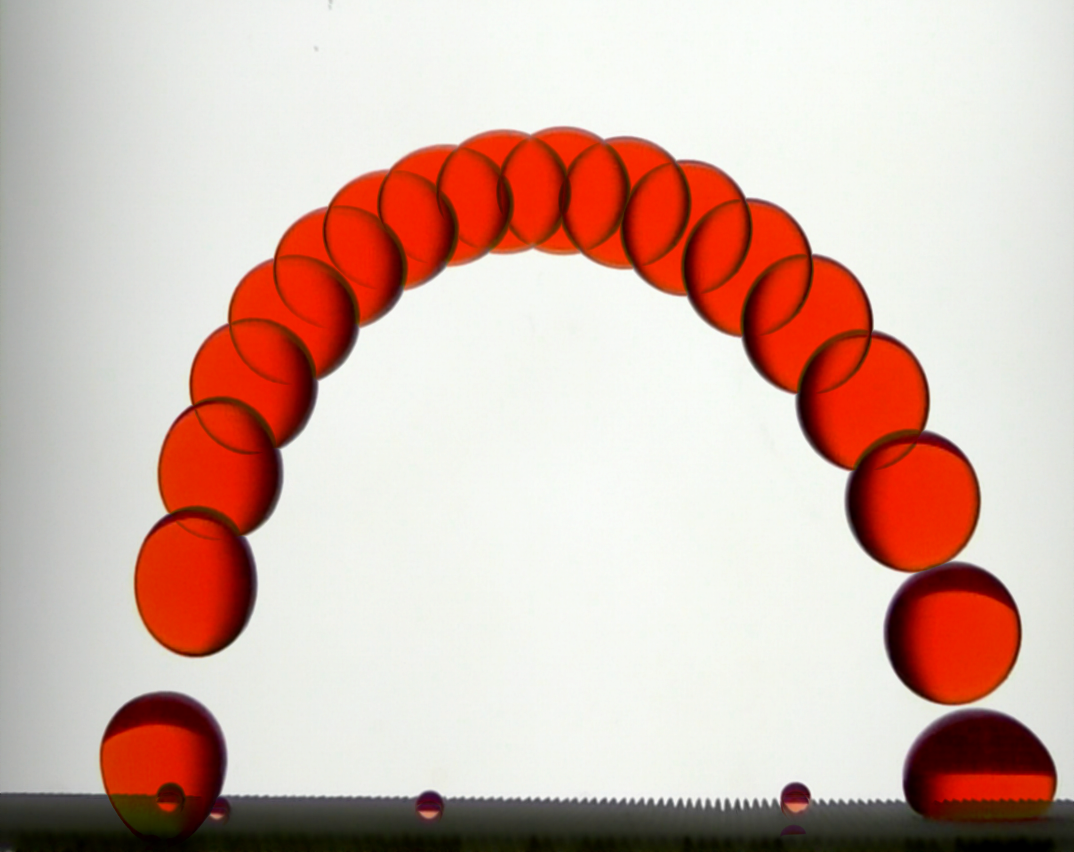
\includegraphics[width=0.5\textwidth]{bounce.png}
\caption{The trajectory of a 0.5 mL drop is captured in a composite image over a single bounce period ($\sim 1.25$ s) presented at $\approx 14$ Hz. Motion of the drop is from left to right. The surface potential of the superhydrophobic dielectric is $\varphi_s = 1.25 \pm 0.41$ kV. \label{fig:bounce}}
\end{figure}

\begin{figure}[htb]
\centering
\resizebox{0.5\textwidth}{!}{%% Creator: Matplotlib, PGF backend
%%
%% To include the figure in your LaTeX document, write
%%   \input{<filename>.pgf}
%%
%% Make sure the required packages are loaded in your preamble
%%   \usepackage{pgf}
%%
%% Figures using additional raster images can only be included by \input if
%% they are in the same directory as the main LaTeX file. For loading figures
%% from other directories you can use the `import` package
%%   \usepackage{import}
%% and then include the figures with
%%   \import{<path to file>}{<filename>.pgf}
%%
%% Matplotlib used the following preamble
%%   \usepackage{fontspec}
%%   \setmainfont{DejaVu Serif}
%%   \setsansfont{DejaVu Sans}
%%   \setmonofont{DejaVu Sans Mono}
%%
\begingroup%
\makeatletter%
\begin{pgfpicture}%
\pgfpathrectangle{\pgfpointorigin}{\pgfqpoint{5.538694in}{3.837899in}}%
\pgfusepath{use as bounding box, clip}%
\begin{pgfscope}%
\pgfsetbuttcap%
\pgfsetmiterjoin%
\definecolor{currentfill}{rgb}{1.000000,1.000000,1.000000}%
\pgfsetfillcolor{currentfill}%
\pgfsetlinewidth{0.000000pt}%
\definecolor{currentstroke}{rgb}{1.000000,1.000000,1.000000}%
\pgfsetstrokecolor{currentstroke}%
\pgfsetdash{}{0pt}%
\pgfpathmoveto{\pgfqpoint{0.000000in}{0.000000in}}%
\pgfpathlineto{\pgfqpoint{5.538694in}{0.000000in}}%
\pgfpathlineto{\pgfqpoint{5.538694in}{3.837899in}}%
\pgfpathlineto{\pgfqpoint{0.000000in}{3.837899in}}%
\pgfpathclose%
\pgfusepath{fill}%
\end{pgfscope}%
\begin{pgfscope}%
\pgfsetbuttcap%
\pgfsetmiterjoin%
\definecolor{currentfill}{rgb}{1.000000,1.000000,1.000000}%
\pgfsetfillcolor{currentfill}%
\pgfsetlinewidth{0.000000pt}%
\definecolor{currentstroke}{rgb}{0.000000,0.000000,0.000000}%
\pgfsetstrokecolor{currentstroke}%
\pgfsetstrokeopacity{0.000000}%
\pgfsetdash{}{0pt}%
\pgfpathmoveto{\pgfqpoint{0.753694in}{0.682899in}}%
\pgfpathlineto{\pgfqpoint{5.403694in}{0.682899in}}%
\pgfpathlineto{\pgfqpoint{5.403694in}{3.702899in}}%
\pgfpathlineto{\pgfqpoint{0.753694in}{3.702899in}}%
\pgfpathclose%
\pgfusepath{fill}%
\end{pgfscope}%
\begin{pgfscope}%
\pgfsetbuttcap%
\pgfsetroundjoin%
\definecolor{currentfill}{rgb}{0.000000,0.000000,0.000000}%
\pgfsetfillcolor{currentfill}%
\pgfsetlinewidth{0.803000pt}%
\definecolor{currentstroke}{rgb}{0.000000,0.000000,0.000000}%
\pgfsetstrokecolor{currentstroke}%
\pgfsetdash{}{0pt}%
\pgfsys@defobject{currentmarker}{\pgfqpoint{0.000000in}{-0.048611in}}{\pgfqpoint{0.000000in}{0.000000in}}{%
\pgfpathmoveto{\pgfqpoint{0.000000in}{0.000000in}}%
\pgfpathlineto{\pgfqpoint{0.000000in}{-0.048611in}}%
\pgfusepath{stroke,fill}%
}%
\begin{pgfscope}%
\pgfsys@transformshift{0.810637in}{0.682899in}%
\pgfsys@useobject{currentmarker}{}%
\end{pgfscope}%
\end{pgfscope}%
\begin{pgfscope}%
\pgftext[x=0.810637in,y=0.585677in,,top]{\rmfamily\fontsize{16.000000}{19.200000}\selectfont \(\displaystyle 0.0\)}%
\end{pgfscope}%
\begin{pgfscope}%
\pgfsetbuttcap%
\pgfsetroundjoin%
\definecolor{currentfill}{rgb}{0.000000,0.000000,0.000000}%
\pgfsetfillcolor{currentfill}%
\pgfsetlinewidth{0.803000pt}%
\definecolor{currentstroke}{rgb}{0.000000,0.000000,0.000000}%
\pgfsetstrokecolor{currentstroke}%
\pgfsetdash{}{0pt}%
\pgfsys@defobject{currentmarker}{\pgfqpoint{0.000000in}{-0.048611in}}{\pgfqpoint{0.000000in}{0.000000in}}{%
\pgfpathmoveto{\pgfqpoint{0.000000in}{0.000000in}}%
\pgfpathlineto{\pgfqpoint{0.000000in}{-0.048611in}}%
\pgfusepath{stroke,fill}%
}%
\begin{pgfscope}%
\pgfsys@transformshift{1.968794in}{0.682899in}%
\pgfsys@useobject{currentmarker}{}%
\end{pgfscope}%
\end{pgfscope}%
\begin{pgfscope}%
\pgftext[x=1.968794in,y=0.585677in,,top]{\rmfamily\fontsize{16.000000}{19.200000}\selectfont \(\displaystyle 0.5\)}%
\end{pgfscope}%
\begin{pgfscope}%
\pgfsetbuttcap%
\pgfsetroundjoin%
\definecolor{currentfill}{rgb}{0.000000,0.000000,0.000000}%
\pgfsetfillcolor{currentfill}%
\pgfsetlinewidth{0.803000pt}%
\definecolor{currentstroke}{rgb}{0.000000,0.000000,0.000000}%
\pgfsetstrokecolor{currentstroke}%
\pgfsetdash{}{0pt}%
\pgfsys@defobject{currentmarker}{\pgfqpoint{0.000000in}{-0.048611in}}{\pgfqpoint{0.000000in}{0.000000in}}{%
\pgfpathmoveto{\pgfqpoint{0.000000in}{0.000000in}}%
\pgfpathlineto{\pgfqpoint{0.000000in}{-0.048611in}}%
\pgfusepath{stroke,fill}%
}%
\begin{pgfscope}%
\pgfsys@transformshift{3.126951in}{0.682899in}%
\pgfsys@useobject{currentmarker}{}%
\end{pgfscope}%
\end{pgfscope}%
\begin{pgfscope}%
\pgftext[x=3.126951in,y=0.585677in,,top]{\rmfamily\fontsize{16.000000}{19.200000}\selectfont \(\displaystyle 1.0\)}%
\end{pgfscope}%
\begin{pgfscope}%
\pgfsetbuttcap%
\pgfsetroundjoin%
\definecolor{currentfill}{rgb}{0.000000,0.000000,0.000000}%
\pgfsetfillcolor{currentfill}%
\pgfsetlinewidth{0.803000pt}%
\definecolor{currentstroke}{rgb}{0.000000,0.000000,0.000000}%
\pgfsetstrokecolor{currentstroke}%
\pgfsetdash{}{0pt}%
\pgfsys@defobject{currentmarker}{\pgfqpoint{0.000000in}{-0.048611in}}{\pgfqpoint{0.000000in}{0.000000in}}{%
\pgfpathmoveto{\pgfqpoint{0.000000in}{0.000000in}}%
\pgfpathlineto{\pgfqpoint{0.000000in}{-0.048611in}}%
\pgfusepath{stroke,fill}%
}%
\begin{pgfscope}%
\pgfsys@transformshift{4.285108in}{0.682899in}%
\pgfsys@useobject{currentmarker}{}%
\end{pgfscope}%
\end{pgfscope}%
\begin{pgfscope}%
\pgftext[x=4.285108in,y=0.585677in,,top]{\rmfamily\fontsize{16.000000}{19.200000}\selectfont \(\displaystyle 1.5\)}%
\end{pgfscope}%
\begin{pgfscope}%
\pgftext[x=3.078694in,y=0.315061in,,top]{\rmfamily\fontsize{16.000000}{19.200000}\selectfont \(\displaystyle t\) (s)}%
\end{pgfscope}%
\begin{pgfscope}%
\pgfsetbuttcap%
\pgfsetroundjoin%
\definecolor{currentfill}{rgb}{0.000000,0.000000,0.000000}%
\pgfsetfillcolor{currentfill}%
\pgfsetlinewidth{0.803000pt}%
\definecolor{currentstroke}{rgb}{0.000000,0.000000,0.000000}%
\pgfsetstrokecolor{currentstroke}%
\pgfsetdash{}{0pt}%
\pgfsys@defobject{currentmarker}{\pgfqpoint{-0.048611in}{0.000000in}}{\pgfqpoint{0.000000in}{0.000000in}}{%
\pgfpathmoveto{\pgfqpoint{0.000000in}{0.000000in}}%
\pgfpathlineto{\pgfqpoint{-0.048611in}{0.000000in}}%
\pgfusepath{stroke,fill}%
}%
\begin{pgfscope}%
\pgfsys@transformshift{0.753694in}{1.164898in}%
\pgfsys@useobject{currentmarker}{}%
\end{pgfscope}%
\end{pgfscope}%
\begin{pgfscope}%
\pgftext[x=0.371059in,y=1.080480in,left,base]{\rmfamily\fontsize{16.000000}{19.200000}\selectfont \(\displaystyle 0.4\)}%
\end{pgfscope}%
\begin{pgfscope}%
\pgfsetbuttcap%
\pgfsetroundjoin%
\definecolor{currentfill}{rgb}{0.000000,0.000000,0.000000}%
\pgfsetfillcolor{currentfill}%
\pgfsetlinewidth{0.803000pt}%
\definecolor{currentstroke}{rgb}{0.000000,0.000000,0.000000}%
\pgfsetstrokecolor{currentstroke}%
\pgfsetdash{}{0pt}%
\pgfsys@defobject{currentmarker}{\pgfqpoint{-0.048611in}{0.000000in}}{\pgfqpoint{0.000000in}{0.000000in}}{%
\pgfpathmoveto{\pgfqpoint{0.000000in}{0.000000in}}%
\pgfpathlineto{\pgfqpoint{-0.048611in}{0.000000in}}%
\pgfusepath{stroke,fill}%
}%
\begin{pgfscope}%
\pgfsys@transformshift{0.753694in}{1.831530in}%
\pgfsys@useobject{currentmarker}{}%
\end{pgfscope}%
\end{pgfscope}%
\begin{pgfscope}%
\pgftext[x=0.371059in,y=1.747111in,left,base]{\rmfamily\fontsize{16.000000}{19.200000}\selectfont \(\displaystyle 0.6\)}%
\end{pgfscope}%
\begin{pgfscope}%
\pgfsetbuttcap%
\pgfsetroundjoin%
\definecolor{currentfill}{rgb}{0.000000,0.000000,0.000000}%
\pgfsetfillcolor{currentfill}%
\pgfsetlinewidth{0.803000pt}%
\definecolor{currentstroke}{rgb}{0.000000,0.000000,0.000000}%
\pgfsetstrokecolor{currentstroke}%
\pgfsetdash{}{0pt}%
\pgfsys@defobject{currentmarker}{\pgfqpoint{-0.048611in}{0.000000in}}{\pgfqpoint{0.000000in}{0.000000in}}{%
\pgfpathmoveto{\pgfqpoint{0.000000in}{0.000000in}}%
\pgfpathlineto{\pgfqpoint{-0.048611in}{0.000000in}}%
\pgfusepath{stroke,fill}%
}%
\begin{pgfscope}%
\pgfsys@transformshift{0.753694in}{2.498162in}%
\pgfsys@useobject{currentmarker}{}%
\end{pgfscope}%
\end{pgfscope}%
\begin{pgfscope}%
\pgftext[x=0.371059in,y=2.413743in,left,base]{\rmfamily\fontsize{16.000000}{19.200000}\selectfont \(\displaystyle 0.8\)}%
\end{pgfscope}%
\begin{pgfscope}%
\pgfsetbuttcap%
\pgfsetroundjoin%
\definecolor{currentfill}{rgb}{0.000000,0.000000,0.000000}%
\pgfsetfillcolor{currentfill}%
\pgfsetlinewidth{0.803000pt}%
\definecolor{currentstroke}{rgb}{0.000000,0.000000,0.000000}%
\pgfsetstrokecolor{currentstroke}%
\pgfsetdash{}{0pt}%
\pgfsys@defobject{currentmarker}{\pgfqpoint{-0.048611in}{0.000000in}}{\pgfqpoint{0.000000in}{0.000000in}}{%
\pgfpathmoveto{\pgfqpoint{0.000000in}{0.000000in}}%
\pgfpathlineto{\pgfqpoint{-0.048611in}{0.000000in}}%
\pgfusepath{stroke,fill}%
}%
\begin{pgfscope}%
\pgfsys@transformshift{0.753694in}{3.164794in}%
\pgfsys@useobject{currentmarker}{}%
\end{pgfscope}%
\end{pgfscope}%
\begin{pgfscope}%
\pgftext[x=0.371059in,y=3.080375in,left,base]{\rmfamily\fontsize{16.000000}{19.200000}\selectfont \(\displaystyle 1.0\)}%
\end{pgfscope}%
\begin{pgfscope}%
\pgftext[x=0.315503in,y=2.192899in,,bottom,rotate=90.000000]{\rmfamily\fontsize{16.000000}{19.200000}\selectfont \(\displaystyle y\) (cm)}%
\end{pgfscope}%
\begin{pgfscope}%
\pgfpathrectangle{\pgfqpoint{0.753694in}{0.682899in}}{\pgfqpoint{4.650000in}{3.020000in}}%
\pgfusepath{clip}%
\pgfsetbuttcap%
\pgfsetroundjoin%
\definecolor{currentfill}{rgb}{1.000000,1.000000,1.000000}%
\pgfsetfillcolor{currentfill}%
\pgfsetlinewidth{1.003750pt}%
\definecolor{currentstroke}{rgb}{0.000000,0.000000,0.000000}%
\pgfsetstrokecolor{currentstroke}%
\pgfsetdash{}{0pt}%
\pgfsys@defobject{currentmarker}{\pgfqpoint{-0.041667in}{-0.041667in}}{\pgfqpoint{0.041667in}{0.041667in}}{%
\pgfpathmoveto{\pgfqpoint{0.000000in}{-0.041667in}}%
\pgfpathcurveto{\pgfqpoint{0.011050in}{-0.041667in}}{\pgfqpoint{0.021649in}{-0.037276in}}{\pgfqpoint{0.029463in}{-0.029463in}}%
\pgfpathcurveto{\pgfqpoint{0.037276in}{-0.021649in}}{\pgfqpoint{0.041667in}{-0.011050in}}{\pgfqpoint{0.041667in}{0.000000in}}%
\pgfpathcurveto{\pgfqpoint{0.041667in}{0.011050in}}{\pgfqpoint{0.037276in}{0.021649in}}{\pgfqpoint{0.029463in}{0.029463in}}%
\pgfpathcurveto{\pgfqpoint{0.021649in}{0.037276in}}{\pgfqpoint{0.011050in}{0.041667in}}{\pgfqpoint{0.000000in}{0.041667in}}%
\pgfpathcurveto{\pgfqpoint{-0.011050in}{0.041667in}}{\pgfqpoint{-0.021649in}{0.037276in}}{\pgfqpoint{-0.029463in}{0.029463in}}%
\pgfpathcurveto{\pgfqpoint{-0.037276in}{0.021649in}}{\pgfqpoint{-0.041667in}{0.011050in}}{\pgfqpoint{-0.041667in}{0.000000in}}%
\pgfpathcurveto{\pgfqpoint{-0.041667in}{-0.011050in}}{\pgfqpoint{-0.037276in}{-0.021649in}}{\pgfqpoint{-0.029463in}{-0.029463in}}%
\pgfpathcurveto{\pgfqpoint{-0.021649in}{-0.037276in}}{\pgfqpoint{-0.011050in}{-0.041667in}}{\pgfqpoint{0.000000in}{-0.041667in}}%
\pgfpathclose%
\pgfusepath{stroke,fill}%
}%
\begin{pgfscope}%
\pgfsys@transformshift{0.965058in}{1.598168in}%
\pgfsys@useobject{currentmarker}{}%
\end{pgfscope}%
\begin{pgfscope}%
\pgfsys@transformshift{0.984361in}{1.740418in}%
\pgfsys@useobject{currentmarker}{}%
\end{pgfscope}%
\begin{pgfscope}%
\pgfsys@transformshift{1.003663in}{1.876859in}%
\pgfsys@useobject{currentmarker}{}%
\end{pgfscope}%
\begin{pgfscope}%
\pgfsys@transformshift{1.022966in}{2.007549in}%
\pgfsys@useobject{currentmarker}{}%
\end{pgfscope}%
\begin{pgfscope}%
\pgfsys@transformshift{1.042269in}{2.132543in}%
\pgfsys@useobject{currentmarker}{}%
\end{pgfscope}%
\begin{pgfscope}%
\pgfsys@transformshift{1.061571in}{2.251895in}%
\pgfsys@useobject{currentmarker}{}%
\end{pgfscope}%
\begin{pgfscope}%
\pgfsys@transformshift{1.080874in}{2.365662in}%
\pgfsys@useobject{currentmarker}{}%
\end{pgfscope}%
\begin{pgfscope}%
\pgfsys@transformshift{1.100176in}{2.473898in}%
\pgfsys@useobject{currentmarker}{}%
\end{pgfscope}%
\begin{pgfscope}%
\pgfsys@transformshift{1.119479in}{2.576660in}%
\pgfsys@useobject{currentmarker}{}%
\end{pgfscope}%
\begin{pgfscope}%
\pgfsys@transformshift{1.138782in}{2.674002in}%
\pgfsys@useobject{currentmarker}{}%
\end{pgfscope}%
\begin{pgfscope}%
\pgfsys@transformshift{1.158084in}{2.765980in}%
\pgfsys@useobject{currentmarker}{}%
\end{pgfscope}%
\begin{pgfscope}%
\pgfsys@transformshift{1.177387in}{2.852650in}%
\pgfsys@useobject{currentmarker}{}%
\end{pgfscope}%
\begin{pgfscope}%
\pgfsys@transformshift{1.196689in}{2.934066in}%
\pgfsys@useobject{currentmarker}{}%
\end{pgfscope}%
\begin{pgfscope}%
\pgfsys@transformshift{1.215992in}{3.010300in}%
\pgfsys@useobject{currentmarker}{}%
\end{pgfscope}%
\begin{pgfscope}%
\pgfsys@transformshift{1.235295in}{3.081404in}%
\pgfsys@useobject{currentmarker}{}%
\end{pgfscope}%
\begin{pgfscope}%
\pgfsys@transformshift{1.254597in}{3.147433in}%
\pgfsys@useobject{currentmarker}{}%
\end{pgfscope}%
\begin{pgfscope}%
\pgfsys@transformshift{1.273900in}{3.208444in}%
\pgfsys@useobject{currentmarker}{}%
\end{pgfscope}%
\begin{pgfscope}%
\pgfsys@transformshift{1.293203in}{3.264491in}%
\pgfsys@useobject{currentmarker}{}%
\end{pgfscope}%
\begin{pgfscope}%
\pgfsys@transformshift{1.312505in}{3.315624in}%
\pgfsys@useobject{currentmarker}{}%
\end{pgfscope}%
\begin{pgfscope}%
\pgfsys@transformshift{1.331808in}{3.361894in}%
\pgfsys@useobject{currentmarker}{}%
\end{pgfscope}%
\begin{pgfscope}%
\pgfsys@transformshift{1.351110in}{3.403345in}%
\pgfsys@useobject{currentmarker}{}%
\end{pgfscope}%
\begin{pgfscope}%
\pgfsys@transformshift{1.370413in}{3.440019in}%
\pgfsys@useobject{currentmarker}{}%
\end{pgfscope}%
\begin{pgfscope}%
\pgfsys@transformshift{1.389716in}{3.471955in}%
\pgfsys@useobject{currentmarker}{}%
\end{pgfscope}%
\begin{pgfscope}%
\pgfsys@transformshift{1.409018in}{3.499184in}%
\pgfsys@useobject{currentmarker}{}%
\end{pgfscope}%
\begin{pgfscope}%
\pgfsys@transformshift{1.428321in}{3.521737in}%
\pgfsys@useobject{currentmarker}{}%
\end{pgfscope}%
\begin{pgfscope}%
\pgfsys@transformshift{1.447623in}{3.539639in}%
\pgfsys@useobject{currentmarker}{}%
\end{pgfscope}%
\begin{pgfscope}%
\pgfsys@transformshift{1.466926in}{3.552911in}%
\pgfsys@useobject{currentmarker}{}%
\end{pgfscope}%
\begin{pgfscope}%
\pgfsys@transformshift{1.486229in}{3.561569in}%
\pgfsys@useobject{currentmarker}{}%
\end{pgfscope}%
\begin{pgfscope}%
\pgfsys@transformshift{1.505531in}{3.565626in}%
\pgfsys@useobject{currentmarker}{}%
\end{pgfscope}%
\begin{pgfscope}%
\pgfsys@transformshift{1.524834in}{3.565093in}%
\pgfsys@useobject{currentmarker}{}%
\end{pgfscope}%
\begin{pgfscope}%
\pgfsys@transformshift{1.544137in}{3.559976in}%
\pgfsys@useobject{currentmarker}{}%
\end{pgfscope}%
\begin{pgfscope}%
\pgfsys@transformshift{1.563439in}{3.550278in}%
\pgfsys@useobject{currentmarker}{}%
\end{pgfscope}%
\begin{pgfscope}%
\pgfsys@transformshift{1.582742in}{3.536001in}%
\pgfsys@useobject{currentmarker}{}%
\end{pgfscope}%
\begin{pgfscope}%
\pgfsys@transformshift{1.602044in}{3.517142in}%
\pgfsys@useobject{currentmarker}{}%
\end{pgfscope}%
\begin{pgfscope}%
\pgfsys@transformshift{1.621347in}{3.493695in}%
\pgfsys@useobject{currentmarker}{}%
\end{pgfscope}%
\begin{pgfscope}%
\pgfsys@transformshift{1.640650in}{3.465648in}%
\pgfsys@useobject{currentmarker}{}%
\end{pgfscope}%
\begin{pgfscope}%
\pgfsys@transformshift{1.659952in}{3.432987in}%
\pgfsys@useobject{currentmarker}{}%
\end{pgfscope}%
\begin{pgfscope}%
\pgfsys@transformshift{1.679255in}{3.395688in}%
\pgfsys@useobject{currentmarker}{}%
\end{pgfscope}%
\begin{pgfscope}%
\pgfsys@transformshift{1.698557in}{3.353728in}%
\pgfsys@useobject{currentmarker}{}%
\end{pgfscope}%
\begin{pgfscope}%
\pgfsys@transformshift{1.717860in}{3.307071in}%
\pgfsys@useobject{currentmarker}{}%
\end{pgfscope}%
\begin{pgfscope}%
\pgfsys@transformshift{1.737163in}{3.255672in}%
\pgfsys@useobject{currentmarker}{}%
\end{pgfscope}%
\begin{pgfscope}%
\pgfsys@transformshift{1.756465in}{3.199471in}%
\pgfsys@useobject{currentmarker}{}%
\end{pgfscope}%
\begin{pgfscope}%
\pgfsys@transformshift{1.775768in}{3.138399in}%
\pgfsys@useobject{currentmarker}{}%
\end{pgfscope}%
\begin{pgfscope}%
\pgfsys@transformshift{1.795071in}{3.072373in}%
\pgfsys@useobject{currentmarker}{}%
\end{pgfscope}%
\begin{pgfscope}%
\pgfsys@transformshift{1.814373in}{3.001296in}%
\pgfsys@useobject{currentmarker}{}%
\end{pgfscope}%
\begin{pgfscope}%
\pgfsys@transformshift{1.833676in}{2.925063in}%
\pgfsys@useobject{currentmarker}{}%
\end{pgfscope}%
\begin{pgfscope}%
\pgfsys@transformshift{1.852978in}{2.843555in}%
\pgfsys@useobject{currentmarker}{}%
\end{pgfscope}%
\begin{pgfscope}%
\pgfsys@transformshift{1.872281in}{2.756646in}%
\pgfsys@useobject{currentmarker}{}%
\end{pgfscope}%
\begin{pgfscope}%
\pgfsys@transformshift{1.891584in}{2.664200in}%
\pgfsys@useobject{currentmarker}{}%
\end{pgfscope}%
\begin{pgfscope}%
\pgfsys@transformshift{1.910886in}{2.566106in}%
\pgfsys@useobject{currentmarker}{}%
\end{pgfscope}%
\begin{pgfscope}%
\pgfsys@transformshift{1.930189in}{2.462126in}%
\pgfsys@useobject{currentmarker}{}%
\end{pgfscope}%
\begin{pgfscope}%
\pgfsys@transformshift{1.949491in}{2.352120in}%
\pgfsys@useobject{currentmarker}{}%
\end{pgfscope}%
\begin{pgfscope}%
\pgfsys@transformshift{1.968794in}{2.235946in}%
\pgfsys@useobject{currentmarker}{}%
\end{pgfscope}%
\begin{pgfscope}%
\pgfsys@transformshift{1.988097in}{2.113464in}%
\pgfsys@useobject{currentmarker}{}%
\end{pgfscope}%
\begin{pgfscope}%
\pgfsys@transformshift{2.007399in}{1.984531in}%
\pgfsys@useobject{currentmarker}{}%
\end{pgfscope}%
\begin{pgfscope}%
\pgfsys@transformshift{2.026702in}{1.849007in}%
\pgfsys@useobject{currentmarker}{}%
\end{pgfscope}%
\begin{pgfscope}%
\pgfsys@transformshift{2.046005in}{1.706752in}%
\pgfsys@useobject{currentmarker}{}%
\end{pgfscope}%
\begin{pgfscope}%
\pgfsys@transformshift{2.065307in}{1.557623in}%
\pgfsys@useobject{currentmarker}{}%
\end{pgfscope}%
\begin{pgfscope}%
\pgfsys@transformshift{2.084610in}{1.401480in}%
\pgfsys@useobject{currentmarker}{}%
\end{pgfscope}%
\begin{pgfscope}%
\pgfsys@transformshift{2.103912in}{1.238182in}%
\pgfsys@useobject{currentmarker}{}%
\end{pgfscope}%
\begin{pgfscope}%
\pgfsys@transformshift{2.123215in}{1.067588in}%
\pgfsys@useobject{currentmarker}{}%
\end{pgfscope}%
\begin{pgfscope}%
\pgfsys@transformshift{2.258333in}{0.933749in}%
\pgfsys@useobject{currentmarker}{}%
\end{pgfscope}%
\begin{pgfscope}%
\pgfsys@transformshift{2.277636in}{1.081897in}%
\pgfsys@useobject{currentmarker}{}%
\end{pgfscope}%
\begin{pgfscope}%
\pgfsys@transformshift{2.296939in}{1.221655in}%
\pgfsys@useobject{currentmarker}{}%
\end{pgfscope}%
\begin{pgfscope}%
\pgfsys@transformshift{2.316241in}{1.353205in}%
\pgfsys@useobject{currentmarker}{}%
\end{pgfscope}%
\begin{pgfscope}%
\pgfsys@transformshift{2.335544in}{1.476730in}%
\pgfsys@useobject{currentmarker}{}%
\end{pgfscope}%
\begin{pgfscope}%
\pgfsys@transformshift{2.354846in}{1.592413in}%
\pgfsys@useobject{currentmarker}{}%
\end{pgfscope}%
\begin{pgfscope}%
\pgfsys@transformshift{2.374149in}{1.700436in}%
\pgfsys@useobject{currentmarker}{}%
\end{pgfscope}%
\begin{pgfscope}%
\pgfsys@transformshift{2.393452in}{1.800980in}%
\pgfsys@useobject{currentmarker}{}%
\end{pgfscope}%
\begin{pgfscope}%
\pgfsys@transformshift{2.412754in}{1.894230in}%
\pgfsys@useobject{currentmarker}{}%
\end{pgfscope}%
\begin{pgfscope}%
\pgfsys@transformshift{2.432057in}{1.980367in}%
\pgfsys@useobject{currentmarker}{}%
\end{pgfscope}%
\begin{pgfscope}%
\pgfsys@transformshift{2.451359in}{2.059575in}%
\pgfsys@useobject{currentmarker}{}%
\end{pgfscope}%
\begin{pgfscope}%
\pgfsys@transformshift{2.470662in}{2.132034in}%
\pgfsys@useobject{currentmarker}{}%
\end{pgfscope}%
\begin{pgfscope}%
\pgfsys@transformshift{2.489965in}{2.197929in}%
\pgfsys@useobject{currentmarker}{}%
\end{pgfscope}%
\begin{pgfscope}%
\pgfsys@transformshift{2.509267in}{2.257577in}%
\pgfsys@useobject{currentmarker}{}%
\end{pgfscope}%
\begin{pgfscope}%
\pgfsys@transformshift{2.528570in}{2.311117in}%
\pgfsys@useobject{currentmarker}{}%
\end{pgfscope}%
\begin{pgfscope}%
\pgfsys@transformshift{2.547873in}{2.358726in}%
\pgfsys@useobject{currentmarker}{}%
\end{pgfscope}%
\begin{pgfscope}%
\pgfsys@transformshift{2.567175in}{2.400566in}%
\pgfsys@useobject{currentmarker}{}%
\end{pgfscope}%
\begin{pgfscope}%
\pgfsys@transformshift{2.586478in}{2.436789in}%
\pgfsys@useobject{currentmarker}{}%
\end{pgfscope}%
\begin{pgfscope}%
\pgfsys@transformshift{2.605780in}{2.467531in}%
\pgfsys@useobject{currentmarker}{}%
\end{pgfscope}%
\begin{pgfscope}%
\pgfsys@transformshift{2.625083in}{2.492913in}%
\pgfsys@useobject{currentmarker}{}%
\end{pgfscope}%
\begin{pgfscope}%
\pgfsys@transformshift{2.644386in}{2.513039in}%
\pgfsys@useobject{currentmarker}{}%
\end{pgfscope}%
\begin{pgfscope}%
\pgfsys@transformshift{2.663688in}{2.527997in}%
\pgfsys@useobject{currentmarker}{}%
\end{pgfscope}%
\begin{pgfscope}%
\pgfsys@transformshift{2.682991in}{2.537855in}%
\pgfsys@useobject{currentmarker}{}%
\end{pgfscope}%
\begin{pgfscope}%
\pgfsys@transformshift{2.702293in}{2.542665in}%
\pgfsys@useobject{currentmarker}{}%
\end{pgfscope}%
\begin{pgfscope}%
\pgfsys@transformshift{2.721596in}{2.542461in}%
\pgfsys@useobject{currentmarker}{}%
\end{pgfscope}%
\begin{pgfscope}%
\pgfsys@transformshift{2.740899in}{2.537254in}%
\pgfsys@useobject{currentmarker}{}%
\end{pgfscope}%
\begin{pgfscope}%
\pgfsys@transformshift{2.760201in}{2.527060in}%
\pgfsys@useobject{currentmarker}{}%
\end{pgfscope}%
\begin{pgfscope}%
\pgfsys@transformshift{2.779504in}{2.511877in}%
\pgfsys@useobject{currentmarker}{}%
\end{pgfscope}%
\begin{pgfscope}%
\pgfsys@transformshift{2.798807in}{2.491684in}%
\pgfsys@useobject{currentmarker}{}%
\end{pgfscope}%
\begin{pgfscope}%
\pgfsys@transformshift{2.818109in}{2.466446in}%
\pgfsys@useobject{currentmarker}{}%
\end{pgfscope}%
\begin{pgfscope}%
\pgfsys@transformshift{2.837412in}{2.436115in}%
\pgfsys@useobject{currentmarker}{}%
\end{pgfscope}%
\begin{pgfscope}%
\pgfsys@transformshift{2.856714in}{2.400628in}%
\pgfsys@useobject{currentmarker}{}%
\end{pgfscope}%
\begin{pgfscope}%
\pgfsys@transformshift{2.876017in}{2.359907in}%
\pgfsys@useobject{currentmarker}{}%
\end{pgfscope}%
\begin{pgfscope}%
\pgfsys@transformshift{2.895320in}{2.313866in}%
\pgfsys@useobject{currentmarker}{}%
\end{pgfscope}%
\begin{pgfscope}%
\pgfsys@transformshift{2.914622in}{2.262406in}%
\pgfsys@useobject{currentmarker}{}%
\end{pgfscope}%
\begin{pgfscope}%
\pgfsys@transformshift{2.933925in}{2.205419in}%
\pgfsys@useobject{currentmarker}{}%
\end{pgfscope}%
\begin{pgfscope}%
\pgfsys@transformshift{2.953227in}{2.142788in}%
\pgfsys@useobject{currentmarker}{}%
\end{pgfscope}%
\begin{pgfscope}%
\pgfsys@transformshift{2.972530in}{2.074423in}%
\pgfsys@useobject{currentmarker}{}%
\end{pgfscope}%
\begin{pgfscope}%
\pgfsys@transformshift{2.991833in}{2.000097in}%
\pgfsys@useobject{currentmarker}{}%
\end{pgfscope}%
\begin{pgfscope}%
\pgfsys@transformshift{3.011135in}{1.919689in}%
\pgfsys@useobject{currentmarker}{}%
\end{pgfscope}%
\begin{pgfscope}%
\pgfsys@transformshift{3.030438in}{1.833074in}%
\pgfsys@useobject{currentmarker}{}%
\end{pgfscope}%
\begin{pgfscope}%
\pgfsys@transformshift{3.049741in}{1.740133in}%
\pgfsys@useobject{currentmarker}{}%
\end{pgfscope}%
\begin{pgfscope}%
\pgfsys@transformshift{3.069043in}{1.640741in}%
\pgfsys@useobject{currentmarker}{}%
\end{pgfscope}%
\begin{pgfscope}%
\pgfsys@transformshift{3.088346in}{1.534778in}%
\pgfsys@useobject{currentmarker}{}%
\end{pgfscope}%
\begin{pgfscope}%
\pgfsys@transformshift{3.107648in}{1.422121in}%
\pgfsys@useobject{currentmarker}{}%
\end{pgfscope}%
\begin{pgfscope}%
\pgfsys@transformshift{3.126951in}{1.302648in}%
\pgfsys@useobject{currentmarker}{}%
\end{pgfscope}%
\begin{pgfscope}%
\pgfsys@transformshift{3.146254in}{1.176237in}%
\pgfsys@useobject{currentmarker}{}%
\end{pgfscope}%
\begin{pgfscope}%
\pgfsys@transformshift{3.165556in}{1.042765in}%
\pgfsys@useobject{currentmarker}{}%
\end{pgfscope}%
\begin{pgfscope}%
\pgfsys@transformshift{3.184859in}{0.902111in}%
\pgfsys@useobject{currentmarker}{}%
\end{pgfscope}%
\begin{pgfscope}%
\pgfsys@transformshift{3.319977in}{1.000224in}%
\pgfsys@useobject{currentmarker}{}%
\end{pgfscope}%
\begin{pgfscope}%
\pgfsys@transformshift{3.339280in}{1.110144in}%
\pgfsys@useobject{currentmarker}{}%
\end{pgfscope}%
\begin{pgfscope}%
\pgfsys@transformshift{3.358582in}{1.212679in}%
\pgfsys@useobject{currentmarker}{}%
\end{pgfscope}%
\begin{pgfscope}%
\pgfsys@transformshift{3.377885in}{1.307828in}%
\pgfsys@useobject{currentmarker}{}%
\end{pgfscope}%
\begin{pgfscope}%
\pgfsys@transformshift{3.397188in}{1.395590in}%
\pgfsys@useobject{currentmarker}{}%
\end{pgfscope}%
\begin{pgfscope}%
\pgfsys@transformshift{3.416490in}{1.475964in}%
\pgfsys@useobject{currentmarker}{}%
\end{pgfscope}%
\begin{pgfscope}%
\pgfsys@transformshift{3.435793in}{1.548949in}%
\pgfsys@useobject{currentmarker}{}%
\end{pgfscope}%
\begin{pgfscope}%
\pgfsys@transformshift{3.455095in}{1.614545in}%
\pgfsys@useobject{currentmarker}{}%
\end{pgfscope}%
\begin{pgfscope}%
\pgfsys@transformshift{3.474398in}{1.672750in}%
\pgfsys@useobject{currentmarker}{}%
\end{pgfscope}%
\begin{pgfscope}%
\pgfsys@transformshift{3.493701in}{1.723564in}%
\pgfsys@useobject{currentmarker}{}%
\end{pgfscope}%
\begin{pgfscope}%
\pgfsys@transformshift{3.513003in}{1.766985in}%
\pgfsys@useobject{currentmarker}{}%
\end{pgfscope}%
\begin{pgfscope}%
\pgfsys@transformshift{3.532306in}{1.803013in}%
\pgfsys@useobject{currentmarker}{}%
\end{pgfscope}%
\begin{pgfscope}%
\pgfsys@transformshift{3.551609in}{1.831648in}%
\pgfsys@useobject{currentmarker}{}%
\end{pgfscope}%
\begin{pgfscope}%
\pgfsys@transformshift{3.570911in}{1.853104in}%
\pgfsys@useobject{currentmarker}{}%
\end{pgfscope}%
\begin{pgfscope}%
\pgfsys@transformshift{3.590214in}{1.867298in}%
\pgfsys@useobject{currentmarker}{}%
\end{pgfscope}%
\begin{pgfscope}%
\pgfsys@transformshift{3.609516in}{1.874203in}%
\pgfsys@useobject{currentmarker}{}%
\end{pgfscope}%
\begin{pgfscope}%
\pgfsys@transformshift{3.628819in}{1.873777in}%
\pgfsys@useobject{currentmarker}{}%
\end{pgfscope}%
\begin{pgfscope}%
\pgfsys@transformshift{3.648122in}{1.865956in}%
\pgfsys@useobject{currentmarker}{}%
\end{pgfscope}%
\begin{pgfscope}%
\pgfsys@transformshift{3.667424in}{1.850659in}%
\pgfsys@useobject{currentmarker}{}%
\end{pgfscope}%
\begin{pgfscope}%
\pgfsys@transformshift{3.686727in}{1.827784in}%
\pgfsys@useobject{currentmarker}{}%
\end{pgfscope}%
\begin{pgfscope}%
\pgfsys@transformshift{3.706029in}{1.797292in}%
\pgfsys@useobject{currentmarker}{}%
\end{pgfscope}%
\begin{pgfscope}%
\pgfsys@transformshift{3.725332in}{1.758840in}%
\pgfsys@useobject{currentmarker}{}%
\end{pgfscope}%
\begin{pgfscope}%
\pgfsys@transformshift{3.744635in}{1.712303in}%
\pgfsys@useobject{currentmarker}{}%
\end{pgfscope}%
\begin{pgfscope}%
\pgfsys@transformshift{3.763937in}{1.657557in}%
\pgfsys@useobject{currentmarker}{}%
\end{pgfscope}%
\begin{pgfscope}%
\pgfsys@transformshift{3.783240in}{1.594476in}%
\pgfsys@useobject{currentmarker}{}%
\end{pgfscope}%
\begin{pgfscope}%
\pgfsys@transformshift{3.802543in}{1.522936in}%
\pgfsys@useobject{currentmarker}{}%
\end{pgfscope}%
\begin{pgfscope}%
\pgfsys@transformshift{3.821845in}{1.442813in}%
\pgfsys@useobject{currentmarker}{}%
\end{pgfscope}%
\begin{pgfscope}%
\pgfsys@transformshift{3.841148in}{1.353980in}%
\pgfsys@useobject{currentmarker}{}%
\end{pgfscope}%
\begin{pgfscope}%
\pgfsys@transformshift{3.860450in}{1.256314in}%
\pgfsys@useobject{currentmarker}{}%
\end{pgfscope}%
\begin{pgfscope}%
\pgfsys@transformshift{3.879753in}{1.149689in}%
\pgfsys@useobject{currentmarker}{}%
\end{pgfscope}%
\begin{pgfscope}%
\pgfsys@transformshift{3.899056in}{1.033981in}%
\pgfsys@useobject{currentmarker}{}%
\end{pgfscope}%
\begin{pgfscope}%
\pgfsys@transformshift{3.918358in}{0.909065in}%
\pgfsys@useobject{currentmarker}{}%
\end{pgfscope}%
\begin{pgfscope}%
\pgfsys@transformshift{4.053477in}{1.011527in}%
\pgfsys@useobject{currentmarker}{}%
\end{pgfscope}%
\begin{pgfscope}%
\pgfsys@transformshift{4.072779in}{1.105166in}%
\pgfsys@useobject{currentmarker}{}%
\end{pgfscope}%
\begin{pgfscope}%
\pgfsys@transformshift{4.092082in}{1.189517in}%
\pgfsys@useobject{currentmarker}{}%
\end{pgfscope}%
\begin{pgfscope}%
\pgfsys@transformshift{4.111384in}{1.264533in}%
\pgfsys@useobject{currentmarker}{}%
\end{pgfscope}%
\begin{pgfscope}%
\pgfsys@transformshift{4.130687in}{1.330171in}%
\pgfsys@useobject{currentmarker}{}%
\end{pgfscope}%
\begin{pgfscope}%
\pgfsys@transformshift{4.149990in}{1.386384in}%
\pgfsys@useobject{currentmarker}{}%
\end{pgfscope}%
\begin{pgfscope}%
\pgfsys@transformshift{4.169292in}{1.433127in}%
\pgfsys@useobject{currentmarker}{}%
\end{pgfscope}%
\begin{pgfscope}%
\pgfsys@transformshift{4.188595in}{1.470356in}%
\pgfsys@useobject{currentmarker}{}%
\end{pgfscope}%
\begin{pgfscope}%
\pgfsys@transformshift{4.207897in}{1.498025in}%
\pgfsys@useobject{currentmarker}{}%
\end{pgfscope}%
\begin{pgfscope}%
\pgfsys@transformshift{4.227200in}{1.516088in}%
\pgfsys@useobject{currentmarker}{}%
\end{pgfscope}%
\begin{pgfscope}%
\pgfsys@transformshift{4.246503in}{1.524501in}%
\pgfsys@useobject{currentmarker}{}%
\end{pgfscope}%
\begin{pgfscope}%
\pgfsys@transformshift{4.265805in}{1.523218in}%
\pgfsys@useobject{currentmarker}{}%
\end{pgfscope}%
\begin{pgfscope}%
\pgfsys@transformshift{4.285108in}{1.512194in}%
\pgfsys@useobject{currentmarker}{}%
\end{pgfscope}%
\begin{pgfscope}%
\pgfsys@transformshift{4.304411in}{1.491383in}%
\pgfsys@useobject{currentmarker}{}%
\end{pgfscope}%
\begin{pgfscope}%
\pgfsys@transformshift{4.323713in}{1.460741in}%
\pgfsys@useobject{currentmarker}{}%
\end{pgfscope}%
\begin{pgfscope}%
\pgfsys@transformshift{4.343016in}{1.420222in}%
\pgfsys@useobject{currentmarker}{}%
\end{pgfscope}%
\begin{pgfscope}%
\pgfsys@transformshift{4.362318in}{1.369781in}%
\pgfsys@useobject{currentmarker}{}%
\end{pgfscope}%
\begin{pgfscope}%
\pgfsys@transformshift{4.381621in}{1.309373in}%
\pgfsys@useobject{currentmarker}{}%
\end{pgfscope}%
\begin{pgfscope}%
\pgfsys@transformshift{4.400924in}{1.238952in}%
\pgfsys@useobject{currentmarker}{}%
\end{pgfscope}%
\begin{pgfscope}%
\pgfsys@transformshift{4.420226in}{1.158473in}%
\pgfsys@useobject{currentmarker}{}%
\end{pgfscope}%
\begin{pgfscope}%
\pgfsys@transformshift{4.439529in}{1.067891in}%
\pgfsys@useobject{currentmarker}{}%
\end{pgfscope}%
\begin{pgfscope}%
\pgfsys@transformshift{4.458831in}{0.967161in}%
\pgfsys@useobject{currentmarker}{}%
\end{pgfscope}%
\begin{pgfscope}%
\pgfsys@transformshift{4.478134in}{0.856237in}%
\pgfsys@useobject{currentmarker}{}%
\end{pgfscope}%
\begin{pgfscope}%
\pgfsys@transformshift{4.613252in}{0.954895in}%
\pgfsys@useobject{currentmarker}{}%
\end{pgfscope}%
\begin{pgfscope}%
\pgfsys@transformshift{4.632555in}{1.018103in}%
\pgfsys@useobject{currentmarker}{}%
\end{pgfscope}%
\begin{pgfscope}%
\pgfsys@transformshift{4.651858in}{1.069344in}%
\pgfsys@useobject{currentmarker}{}%
\end{pgfscope}%
\begin{pgfscope}%
\pgfsys@transformshift{4.671160in}{1.108408in}%
\pgfsys@useobject{currentmarker}{}%
\end{pgfscope}%
\begin{pgfscope}%
\pgfsys@transformshift{4.690463in}{1.135086in}%
\pgfsys@useobject{currentmarker}{}%
\end{pgfscope}%
\begin{pgfscope}%
\pgfsys@transformshift{4.709765in}{1.149169in}%
\pgfsys@useobject{currentmarker}{}%
\end{pgfscope}%
\begin{pgfscope}%
\pgfsys@transformshift{4.729068in}{1.150446in}%
\pgfsys@useobject{currentmarker}{}%
\end{pgfscope}%
\begin{pgfscope}%
\pgfsys@transformshift{4.748371in}{1.138708in}%
\pgfsys@useobject{currentmarker}{}%
\end{pgfscope}%
\begin{pgfscope}%
\pgfsys@transformshift{4.767673in}{1.113745in}%
\pgfsys@useobject{currentmarker}{}%
\end{pgfscope}%
\begin{pgfscope}%
\pgfsys@transformshift{4.786976in}{1.075349in}%
\pgfsys@useobject{currentmarker}{}%
\end{pgfscope}%
\begin{pgfscope}%
\pgfsys@transformshift{4.806279in}{1.023308in}%
\pgfsys@useobject{currentmarker}{}%
\end{pgfscope}%
\begin{pgfscope}%
\pgfsys@transformshift{4.825581in}{0.957415in}%
\pgfsys@useobject{currentmarker}{}%
\end{pgfscope}%
\begin{pgfscope}%
\pgfsys@transformshift{4.844884in}{0.877458in}%
\pgfsys@useobject{currentmarker}{}%
\end{pgfscope}%
\begin{pgfscope}%
\pgfsys@transformshift{4.960699in}{0.820172in}%
\pgfsys@useobject{currentmarker}{}%
\end{pgfscope}%
\begin{pgfscope}%
\pgfsys@transformshift{4.980002in}{0.899855in}%
\pgfsys@useobject{currentmarker}{}%
\end{pgfscope}%
\begin{pgfscope}%
\pgfsys@transformshift{4.999305in}{0.965837in}%
\pgfsys@useobject{currentmarker}{}%
\end{pgfscope}%
\begin{pgfscope}%
\pgfsys@transformshift{5.018607in}{1.017977in}%
\pgfsys@useobject{currentmarker}{}%
\end{pgfscope}%
\begin{pgfscope}%
\pgfsys@transformshift{5.037910in}{1.056137in}%
\pgfsys@useobject{currentmarker}{}%
\end{pgfscope}%
\begin{pgfscope}%
\pgfsys@transformshift{5.057213in}{1.080177in}%
\pgfsys@useobject{currentmarker}{}%
\end{pgfscope}%
\begin{pgfscope}%
\pgfsys@transformshift{5.076515in}{1.089957in}%
\pgfsys@useobject{currentmarker}{}%
\end{pgfscope}%
\begin{pgfscope}%
\pgfsys@transformshift{5.095818in}{1.085339in}%
\pgfsys@useobject{currentmarker}{}%
\end{pgfscope}%
\begin{pgfscope}%
\pgfsys@transformshift{5.115120in}{1.066183in}%
\pgfsys@useobject{currentmarker}{}%
\end{pgfscope}%
\begin{pgfscope}%
\pgfsys@transformshift{5.134423in}{1.032348in}%
\pgfsys@useobject{currentmarker}{}%
\end{pgfscope}%
\begin{pgfscope}%
\pgfsys@transformshift{5.153726in}{0.983697in}%
\pgfsys@useobject{currentmarker}{}%
\end{pgfscope}%
\begin{pgfscope}%
\pgfsys@transformshift{5.173028in}{0.920090in}%
\pgfsys@useobject{currentmarker}{}%
\end{pgfscope}%
\begin{pgfscope}%
\pgfsys@transformshift{5.192331in}{0.841387in}%
\pgfsys@useobject{currentmarker}{}%
\end{pgfscope}%
\end{pgfscope}%
\begin{pgfscope}%
\pgfpathrectangle{\pgfqpoint{0.753694in}{0.682899in}}{\pgfqpoint{4.650000in}{3.020000in}}%
\pgfusepath{clip}%
\pgfsetbuttcap%
\pgfsetroundjoin%
\definecolor{currentfill}{rgb}{0.121569,0.466667,0.705882}%
\pgfsetfillcolor{currentfill}%
\pgfsetlinewidth{1.003750pt}%
\definecolor{currentstroke}{rgb}{0.121569,0.466667,0.705882}%
\pgfsetstrokecolor{currentstroke}%
\pgfsetdash{}{0pt}%
\pgfsys@defobject{currentmarker}{\pgfqpoint{-0.041667in}{-0.041667in}}{\pgfqpoint{0.041667in}{0.041667in}}{%
\pgfpathmoveto{\pgfqpoint{0.000000in}{-0.041667in}}%
\pgfpathcurveto{\pgfqpoint{0.011050in}{-0.041667in}}{\pgfqpoint{0.021649in}{-0.037276in}}{\pgfqpoint{0.029463in}{-0.029463in}}%
\pgfpathcurveto{\pgfqpoint{0.037276in}{-0.021649in}}{\pgfqpoint{0.041667in}{-0.011050in}}{\pgfqpoint{0.041667in}{0.000000in}}%
\pgfpathcurveto{\pgfqpoint{0.041667in}{0.011050in}}{\pgfqpoint{0.037276in}{0.021649in}}{\pgfqpoint{0.029463in}{0.029463in}}%
\pgfpathcurveto{\pgfqpoint{0.021649in}{0.037276in}}{\pgfqpoint{0.011050in}{0.041667in}}{\pgfqpoint{0.000000in}{0.041667in}}%
\pgfpathcurveto{\pgfqpoint{-0.011050in}{0.041667in}}{\pgfqpoint{-0.021649in}{0.037276in}}{\pgfqpoint{-0.029463in}{0.029463in}}%
\pgfpathcurveto{\pgfqpoint{-0.037276in}{0.021649in}}{\pgfqpoint{-0.041667in}{0.011050in}}{\pgfqpoint{-0.041667in}{0.000000in}}%
\pgfpathcurveto{\pgfqpoint{-0.041667in}{-0.011050in}}{\pgfqpoint{-0.037276in}{-0.021649in}}{\pgfqpoint{-0.029463in}{-0.029463in}}%
\pgfpathcurveto{\pgfqpoint{-0.021649in}{-0.037276in}}{\pgfqpoint{-0.011050in}{-0.041667in}}{\pgfqpoint{0.000000in}{-0.041667in}}%
\pgfpathclose%
\pgfusepath{stroke,fill}%
}%
\begin{pgfscope}%
\pgfsys@transformshift{0.965058in}{1.598168in}%
\pgfsys@useobject{currentmarker}{}%
\end{pgfscope}%
\begin{pgfscope}%
\pgfsys@transformshift{2.123215in}{1.067588in}%
\pgfsys@useobject{currentmarker}{}%
\end{pgfscope}%
\begin{pgfscope}%
\pgfsys@transformshift{2.258333in}{0.933749in}%
\pgfsys@useobject{currentmarker}{}%
\end{pgfscope}%
\begin{pgfscope}%
\pgfsys@transformshift{3.184859in}{0.902111in}%
\pgfsys@useobject{currentmarker}{}%
\end{pgfscope}%
\begin{pgfscope}%
\pgfsys@transformshift{3.319977in}{1.000224in}%
\pgfsys@useobject{currentmarker}{}%
\end{pgfscope}%
\begin{pgfscope}%
\pgfsys@transformshift{3.918358in}{0.909065in}%
\pgfsys@useobject{currentmarker}{}%
\end{pgfscope}%
\begin{pgfscope}%
\pgfsys@transformshift{4.053477in}{1.011527in}%
\pgfsys@useobject{currentmarker}{}%
\end{pgfscope}%
\begin{pgfscope}%
\pgfsys@transformshift{4.478134in}{0.856237in}%
\pgfsys@useobject{currentmarker}{}%
\end{pgfscope}%
\begin{pgfscope}%
\pgfsys@transformshift{4.613252in}{0.954895in}%
\pgfsys@useobject{currentmarker}{}%
\end{pgfscope}%
\begin{pgfscope}%
\pgfsys@transformshift{4.844884in}{0.877458in}%
\pgfsys@useobject{currentmarker}{}%
\end{pgfscope}%
\begin{pgfscope}%
\pgfsys@transformshift{4.960699in}{0.820172in}%
\pgfsys@useobject{currentmarker}{}%
\end{pgfscope}%
\begin{pgfscope}%
\pgfsys@transformshift{5.192331in}{0.841387in}%
\pgfsys@useobject{currentmarker}{}%
\end{pgfscope}%
\end{pgfscope}%
\begin{pgfscope}%
\pgfsetrectcap%
\pgfsetmiterjoin%
\pgfsetlinewidth{0.803000pt}%
\definecolor{currentstroke}{rgb}{0.501961,0.501961,0.501961}%
\pgfsetstrokecolor{currentstroke}%
\pgfsetdash{}{0pt}%
\pgfpathmoveto{\pgfqpoint{0.753694in}{0.682899in}}%
\pgfpathlineto{\pgfqpoint{0.753694in}{3.702899in}}%
\pgfusepath{stroke}%
\end{pgfscope}%
\begin{pgfscope}%
\pgfsetrectcap%
\pgfsetmiterjoin%
\pgfsetlinewidth{0.803000pt}%
\definecolor{currentstroke}{rgb}{0.501961,0.501961,0.501961}%
\pgfsetstrokecolor{currentstroke}%
\pgfsetdash{}{0pt}%
\pgfpathmoveto{\pgfqpoint{5.403694in}{0.682899in}}%
\pgfpathlineto{\pgfqpoint{5.403694in}{3.702899in}}%
\pgfusepath{stroke}%
\end{pgfscope}%
\begin{pgfscope}%
\pgfsetrectcap%
\pgfsetmiterjoin%
\pgfsetlinewidth{0.803000pt}%
\definecolor{currentstroke}{rgb}{0.501961,0.501961,0.501961}%
\pgfsetstrokecolor{currentstroke}%
\pgfsetdash{}{0pt}%
\pgfpathmoveto{\pgfqpoint{0.753694in}{0.682899in}}%
\pgfpathlineto{\pgfqpoint{5.403694in}{0.682899in}}%
\pgfusepath{stroke}%
\end{pgfscope}%
\begin{pgfscope}%
\pgfsetrectcap%
\pgfsetmiterjoin%
\pgfsetlinewidth{0.803000pt}%
\definecolor{currentstroke}{rgb}{0.501961,0.501961,0.501961}%
\pgfsetstrokecolor{currentstroke}%
\pgfsetdash{}{0pt}%
\pgfpathmoveto{\pgfqpoint{0.753694in}{3.702899in}}%
\pgfpathlineto{\pgfqpoint{5.403694in}{3.702899in}}%
\pgfusepath{stroke}%
\end{pgfscope}%
\end{pgfpicture}%
\makeatother%
\endgroup%
}
\caption{The trajectory time-series of a 0.05 mL drop with surface potential $\varphi_s = 0.75 \pm 0.5$ kV. \label{fig:bounce_time}}
\end{figure}

Preliminary observations of the drop bouncing behavior include:
\begin{itemize}
\item Observed maximum drop (de-)accelerations are on the order of $\sim$0.3 m/s$^2$ for a range of drop volumes $0.03 \lessapprox V_d \lessapprox 0.5$ mL.
\item The water drops are attracted to regions of high electric field. Horizontal (surface plane parallel) translations usually orbit or oscillate about some central position during the experiment. Presumably this central position is a local maxima of the electric field. For especially small drops close to the spontaneous drop jump limit, identified by Attari \emph{et al.} \citep{attari_puddle_2016} and Ahvad \emph{et al.} \citep{avhad_numerical_2020} as $V_d \sim$ 0.01 mL, the drops do not jump but instead translate across the surface in a rolling regime. This oscillatory translation is damped and eventually arrested by contact line hysteresis and viscous dissipation.
\item The drops have net free charge. In experiments of multiple simultaneous drop jumps the drops repel each other as they bounce or roll in orbital motion around regions of high field.
\item The magnitude of the drop trajectory maxima (the trajectory apoapsis) is related to the drop volume, initial jump velocity, and electric field strength.
\end{itemize}

It is well known that water acquires positive free charge when in contact with certain polymers, especially polytetrafluoroethylene (PTFE), through a process called contact charging. \cite{langmuir_surface_1938} PTFE, by contrast, tends to readily acquire negative charge by contact with water. The superhydrophobic surfaces used in the spontaneous drop jump experiments have thin (nanometric) PTFE coatings, and we observe that it is easy to produce significant surface potentials $\varphi_s \sim$ 100-500 V by simply flowing streams of distilled water over them. We suspect that these surfaces have sometimes unintentially become charged during our cleaning processes. This unintentional charging eventually led to our fortuitious initial observations of electro-bouncing phenomena. In the methods section we discuss a controlled experiment to recreate the phenomenon. A study of water on PTFE contact charging phenomenon was conducted by Yatsuzuka \emph{et al.} \cite{yatsuzuka_electrification_1994} who suggest that this process results from formation of an electrical double layer driven by selective adsorption of ($\mbox{OH}^-$) ions at the polymer surface. Other recent work supports this hypothesis. \cite{beattie_intrinsic_2006, strazdaite_water_2015} 

The source of the net free charge on the drops is another issue. The drop charge could be due to the contact charging mechanism mentioned previously. NASA flight engineer Don Pettit discusses the problem of low-gravity flow induced charging of liquids resulting ultimately from contact charging phenomenon. \cite{pettit_donald_flow_1996} However, we suspect that a more likely mechanism for the drop charge is field-induced charging occuring due to physical breakup of a conductor with a field-induced dipole. In our work this might occur when a drop is deposited on the charged surface by a grounded syringe. Field-induced charging is at work in the famous Kelvin thunderstorm and is applied in inkjet and electrospray technologies, where in each case the breakup is by the Rayleigh-Plateau instability. Notably, in Pettit's aforementioned discussion of contact charging of liquids in low-gravity, he remarks on accidental electrostatic `hula-ing' of silicone oil drops when ejected from a syringe in the vicinity of a highly-charged polymer surface during an experiment conducted aboard STS-5 by Space Shuttle mission specialist Joseph Allen. \cite{pettit_donald_flow_1996} Relatedly, in a series of informal and somewhat whimsical experiments, Pettit himself electrostatically orbited small water drops around a triboelectrically charged PTFE knitting needle while aboard the International Space Station (ISS) during expedition 30\textbackslash 31. \cite{stevenson_electrostatic_2015} Again, the drop charge is likely field-induced. Regardless of the charging mechanism the drops tend to remain charged over time. Given the large roughness ratio of projected to actual surface area of the superhydrophobic surfaces used in the experiment, and given that the drop initially rests upon the surface in a Cassie-Baxter state, there exists a somewhat electrically resistive air layer which insulates the drop in spite of the large floating potential.

The electro-drop bounce phenomenon may have useful applications in a low-gravity environment, generally to tackle seperation of droplets from a two-phase flow. Removal of satellite droplets produced during pipetting in wet-lab research aboard the International Space Station (ISS) has been recently suggested as an application of this work. \cite{turner_mitigation_2019} Droplets can become spontaneously charged by contact with standard micropipette tips \citep{choi_spontaneous_2013} and this free charge can be leveraged for the purpose of phase separation in low-gravity. These drops are easily inhaled and currently present a safety hazard to astronauts. The application of this work could allow future wet-lab work to proceed outside of the burdensome constraints of a glovebox environment, thus increasing the yield of such research aboard ISS to the benefit of humanity.

\section{Theory}
\subsection{Equation of Motion}
We develop here a simple 1-dimensional model of the dynamics of free falling drops dominated by electrostatic forces. We treat a drop as a particle with radius $R_d$, which translates vertically along the central axis of a charged dielectric square sheet substrate. The equation of motion for this system is given by,
\begin{equation}
m y'' = - F_D - F_E,
\label{gov_eqn}
\end{equation}
subject to
\begin{equation}
y(0) = R_d, \hspace{5 mm} \mbox{and} \hspace{5 mm} y'(0) = U_0,
\end{equation}
where $m$ is the drop mass, $y'' = d^2 y/d t^2$ is the drop acceleration, $F_D$ is the drag force which always opposes motion, and $F_E$ is the electrostatic force. The assumed initial conditions are such that when $\mathbb{B}\mbox{o}$ is suddenly reduced at the start of the drop tower free-fall period, the drop jumps with instantaneous initial velocity $U_0$ from its 1-$g_0$ resting position of $R_d$ at $t=0$. The dynamical system is sketched schematically in Figure \ref{fig:apparatus}. We now define models for each of the forces in this equation.

\begin{figure}[ht]
\centering
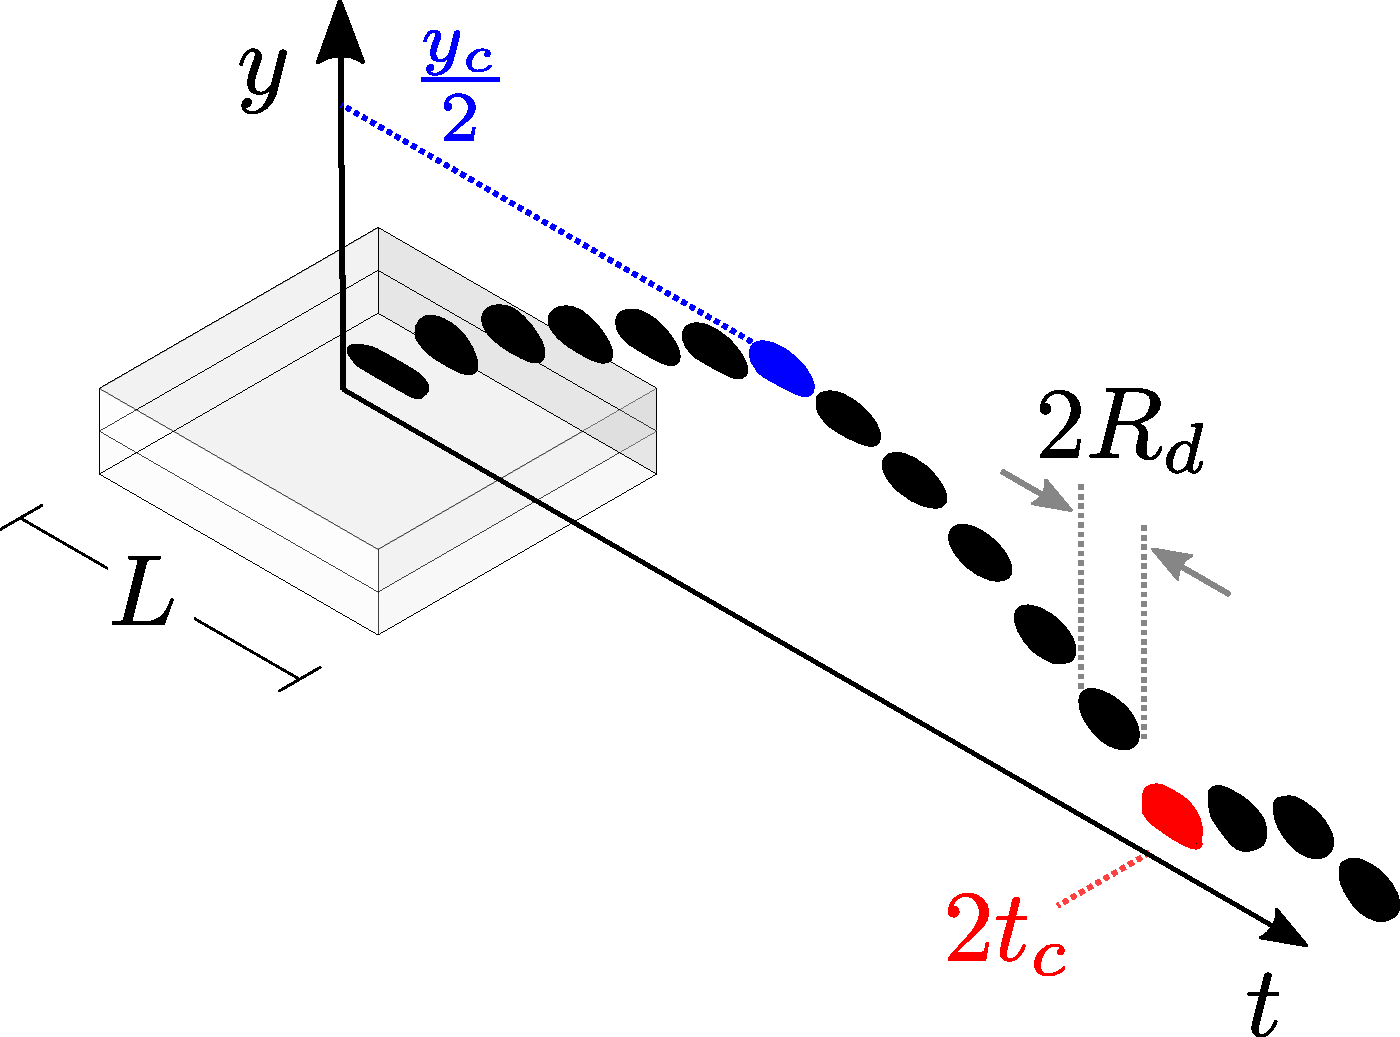
\includegraphics[width=0.45\textwidth]{../figures/apparatus3.pdf}
\caption{Schematic representation of drop jump with return and rebound from an electrically charged superhydrophobic substrate. The characteristic time and length scales $t_c$ and $y_c$ describe the time of flight and apoapse associated with the drop trajectory. $L$ denotes the length scale characteristic of the charged superhydrophobic substrate.}
\label{fig:apparatus}
\end{figure}

For the intermediate range of Reynolds numbers $1 \leq \mathbb{R}\mbox{e} \equiv 2UR_d / \nu \leq 50 $ observed in our experiments, we assume the force of drag acting on the drop to be quadratic, with $\nu$ being the kinematic viscosity.

In modeling the electrostatic force we begin with the standard leaky dielectric approximation for an incompressible fluid. \cite{saville_electrohydrodynamics_1997} Supposing that electrical forces acting on free charges and dipoles in a fluid are transferred directly to the fluid itself, the electric body force density $\mathbf{f}_E$ will be the divergence of the Maxwell stress tensor $\tau_m $,
\begin{eqnarray} \label{e_force}
 \mathbf{f}_E &=& \nabla \cdot \tau_m \nonumber \\ 
 &=& \rho_e \mathbf{E} + \frac{1}{2} \left| E \right|^2 \nabla \epsilon ,
\end{eqnarray}
where $\rho_e$ is the charge density, $\mathbf{E}$ is the electric field, and $\epsilon$ is the dielectric permittivity. The first term on the right hand side of this expression is the well known Coulombic force or electrophoretic force, which arises from the presence of free charge in an external electric field. We expect this term to dominate the electric force in a DC field. The second term is the force arising from polarization stresses due to a nonuniform field acting across a gradient in permittivity. This force is widely termed the dielectrophoretic (DEP) force. 

By comparing DEP and Coulombic forces we note that a condition to neglect the DEP force is
\begin{eqnarray}
\left| \frac{ \kappa_w \epsilon_0 K R_d^2 E_0}{q} \right| \ll 1, \nonumber
\end{eqnarray}
where $\epsilon_0$ is the vacuum permittivity, and $\kappa_w$ and $\kappa_a$ are the relative dielectric constants of the water particle and air host fluid, respectively and in general $\kappa = \epsilon/\epsilon_0$. Here it is convenient to use the simplifying shorthand $K = \frac{\kappa_w - \kappa_a}{\kappa_w + 2 \kappa_a}$, known as the Clausius-Mossotti factor. In cases where $K <$ 0, or $K>$ 0 the particle will be respectively repelled or attracted to regions of strong field. 
This conditions prevails in our experiments and we henceforth neglect the DEP force. Inasmuch as internal flows and small oscillations of the drop interface affect the drop shape and charge distribution we neglect their effects on the dynamics of the drop because they appear primarily as a correction to the DEP force (and to a lesser effect to the drag). Thus only the Coulombic force density remains. When integrated over the drop volume this yields for the electrostatic force $\mathbf{F}_E = q \mathbf{E}$. 

When the drop is close to the dielectric surface, the free charge on the drop will tend to induce polarization of the dielectric which perturbs the electric field. The polarization bound charge in the dielectric will be of the opposite sign of the free drop charge and thus there will be a force of attraction. This so-called image force is a correction to the Coulomb force due to the external electric field only, and can be found by a Green's Function solution of Laplace's equation for the electric field, the `method of images'. \cite{david_j._griffiths_introduction_1999} This resulting image force $\mathbf{F}_I$ is given by
\begin{equation}
\mathbf{F}_I = \frac{k q^2}{16 \pi \epsilon_0} y^{-2} \hat{\mathbf{j}},
\label{image_force}
\end{equation}
where the factor $k$ is a function of the dielectric surface susceptibility $k = \frac{\chi_e}{\chi_e + 2}$, $\chi_e = \kappa_d - 1$, $\kappa_d$ is the relative dielectric constant of the dielectric substrate, and $\hat{\mathbf{j}}$ is a unit vector normal to the dielectric surface.

By substituting Equation \ref{image_force} into \ref{e_force} we have for a single drop
\begin{eqnarray}
 \mathbf{F}_E &=& q \mathbf{E} + \mathbf{F}_I \nonumber \\
 &=& q \mathbf{E} + \frac{k q^2}{16 \pi \epsilon_0 } y^{-2} \hat{\mathbf{j}} \label{e_forces}
\end{eqnarray}

Thus the 1-D governing Equation \ref{gov_eqn}, becomes
\begin{equation}
 \label{gov_eqn_subs}
m y'' = - \frac{1}{2} C_D \rho A {y'}^2 - q E - \frac{k q^2}{16 \pi \epsilon_0} y^{-2},
\end{equation}
subject to
\begin{equation*}
y(0) = R_d, \hspace{5 mm} \mbox{and} \hspace{5 mm} y'(0) = U_0 .
\end{equation*}

\subsection{Electric Field}
If we consider the charged dielectric surface of our experiments to be a square sheet of charge lying in the $xz$-plane of width $L$, the symmetry of the problem lets us obtain the $y$-component of the electric field $\mathbf{E}$ by direct integration (as a superposition of line charges) \citep{david_j._griffiths_introduction_1999} as
\begin{equation}
\label{e_field}
E = \frac{\sigma}{ \pi \epsilon_0} \tan^{-1} \left( \frac{L^2}{y \sqrt{2L^2 + 4y^2}}\right)
,\end{equation}
where $\sigma$ is the surface charge density. We note that this 1D model of the electric field is valid when $R_d \ll L$, which will be true for cases of small drops `far' from the dielectric surface. 

By making some simplifying assumptions we gain some insight about the limiting behavior of this field. In the limit $y/L \ll 1$ Equation \ref{e_field} reduces to
\begin{equation}
\label{near_field}
E \approx \frac{\sigma}{2 \epsilon_0} = E_0,
\end{equation}
where $E_0$ is the characteristic electric field. This field is constant and equivalent to the electric field due to an infinite plane of charge. In the limit of $y/L \gg 1$, Equation \ref{e_field} reduces to the familiar electric field due to a point charge
\begin{equation}
\label{far_field}
E \approx \frac{1}{2\pi}  L^2 E_0 y^{-2}.
\end{equation}
Equation \ref{e_field} with both regimes given by \ref{near_field} and \ref{far_field} are identified in Figure \ref{fig:E0}.
\begin{figure}[h]
	\centering
    \resizebox{0.5\textwidth}{!}{%% Creator: Matplotlib, PGF backend
%%
%% To include the figure in your LaTeX document, write
%%   \input{<filename>.pgf}
%%
%% Make sure the required packages are loaded in your preamble
%%   \usepackage{pgf}
%%
%% Figures using additional raster images can only be included by \input if
%% they are in the same directory as the main LaTeX file. For loading figures
%% from other directories you can use the `import` package
%%   \usepackage{import}
%% and then include the figures with
%%   \import{<path to file>}{<filename>.pgf}
%%
%% Matplotlib used the following preamble
%%   \usepackage{fontspec}
%%   \setmainfont{DejaVu Serif}
%%   \setsansfont{DejaVu Sans}
%%   \setmonofont{DejaVu Sans Mono}
%%
\begingroup%
\makeatletter%
\begin{pgfpicture}%
\pgfpathrectangle{\pgfpointorigin}{\pgfqpoint{5.698771in}{3.862421in}}%
\pgfusepath{use as bounding box, clip}%
\begin{pgfscope}%
\pgfsetbuttcap%
\pgfsetmiterjoin%
\definecolor{currentfill}{rgb}{1.000000,1.000000,1.000000}%
\pgfsetfillcolor{currentfill}%
\pgfsetlinewidth{0.000000pt}%
\definecolor{currentstroke}{rgb}{1.000000,1.000000,1.000000}%
\pgfsetstrokecolor{currentstroke}%
\pgfsetdash{}{0pt}%
\pgfpathmoveto{\pgfqpoint{0.000000in}{0.000000in}}%
\pgfpathlineto{\pgfqpoint{5.698771in}{0.000000in}}%
\pgfpathlineto{\pgfqpoint{5.698771in}{3.862421in}}%
\pgfpathlineto{\pgfqpoint{0.000000in}{3.862421in}}%
\pgfpathclose%
\pgfusepath{fill}%
\end{pgfscope}%
\begin{pgfscope}%
\pgfsetbuttcap%
\pgfsetmiterjoin%
\definecolor{currentfill}{rgb}{1.000000,1.000000,1.000000}%
\pgfsetfillcolor{currentfill}%
\pgfsetlinewidth{0.000000pt}%
\definecolor{currentstroke}{rgb}{0.000000,0.000000,0.000000}%
\pgfsetstrokecolor{currentstroke}%
\pgfsetstrokeopacity{0.000000}%
\pgfsetdash{}{0pt}%
\pgfpathmoveto{\pgfqpoint{0.913771in}{0.707421in}}%
\pgfpathlineto{\pgfqpoint{5.563771in}{0.707421in}}%
\pgfpathlineto{\pgfqpoint{5.563771in}{3.727421in}}%
\pgfpathlineto{\pgfqpoint{0.913771in}{3.727421in}}%
\pgfpathclose%
\pgfusepath{fill}%
\end{pgfscope}%
\begin{pgfscope}%
\pgfsetbuttcap%
\pgfsetroundjoin%
\definecolor{currentfill}{rgb}{0.000000,0.000000,0.000000}%
\pgfsetfillcolor{currentfill}%
\pgfsetlinewidth{0.803000pt}%
\definecolor{currentstroke}{rgb}{0.000000,0.000000,0.000000}%
\pgfsetstrokecolor{currentstroke}%
\pgfsetdash{}{0pt}%
\pgfsys@defobject{currentmarker}{\pgfqpoint{0.000000in}{-0.048611in}}{\pgfqpoint{0.000000in}{0.000000in}}{%
\pgfpathmoveto{\pgfqpoint{0.000000in}{0.000000in}}%
\pgfpathlineto{\pgfqpoint{0.000000in}{-0.048611in}}%
\pgfusepath{stroke,fill}%
}%
\begin{pgfscope}%
\pgfsys@transformshift{2.445783in}{0.707421in}%
\pgfsys@useobject{currentmarker}{}%
\end{pgfscope}%
\end{pgfscope}%
\begin{pgfscope}%
\pgftext[x=2.445783in,y=0.610199in,,top]{\rmfamily\fontsize{16.000000}{19.200000}\selectfont \(\displaystyle 10^{-1}\)}%
\end{pgfscope}%
\begin{pgfscope}%
\pgfsetbuttcap%
\pgfsetroundjoin%
\definecolor{currentfill}{rgb}{0.000000,0.000000,0.000000}%
\pgfsetfillcolor{currentfill}%
\pgfsetlinewidth{0.803000pt}%
\definecolor{currentstroke}{rgb}{0.000000,0.000000,0.000000}%
\pgfsetstrokecolor{currentstroke}%
\pgfsetdash{}{0pt}%
\pgfsys@defobject{currentmarker}{\pgfqpoint{0.000000in}{-0.048611in}}{\pgfqpoint{0.000000in}{0.000000in}}{%
\pgfpathmoveto{\pgfqpoint{0.000000in}{0.000000in}}%
\pgfpathlineto{\pgfqpoint{0.000000in}{-0.048611in}}%
\pgfusepath{stroke,fill}%
}%
\begin{pgfscope}%
\pgfsys@transformshift{4.070370in}{0.707421in}%
\pgfsys@useobject{currentmarker}{}%
\end{pgfscope}%
\end{pgfscope}%
\begin{pgfscope}%
\pgftext[x=4.070370in,y=0.610199in,,top]{\rmfamily\fontsize{16.000000}{19.200000}\selectfont \(\displaystyle 10^{0}\)}%
\end{pgfscope}%
\begin{pgfscope}%
\pgfsetbuttcap%
\pgfsetroundjoin%
\definecolor{currentfill}{rgb}{0.000000,0.000000,0.000000}%
\pgfsetfillcolor{currentfill}%
\pgfsetlinewidth{0.602250pt}%
\definecolor{currentstroke}{rgb}{0.000000,0.000000,0.000000}%
\pgfsetstrokecolor{currentstroke}%
\pgfsetdash{}{0pt}%
\pgfsys@defobject{currentmarker}{\pgfqpoint{0.000000in}{-0.027778in}}{\pgfqpoint{0.000000in}{0.000000in}}{%
\pgfpathmoveto{\pgfqpoint{0.000000in}{0.000000in}}%
\pgfpathlineto{\pgfqpoint{0.000000in}{-0.027778in}}%
\pgfusepath{stroke,fill}%
}%
\begin{pgfscope}%
\pgfsys@transformshift{1.310245in}{0.707421in}%
\pgfsys@useobject{currentmarker}{}%
\end{pgfscope}%
\end{pgfscope}%
\begin{pgfscope}%
\pgfsetbuttcap%
\pgfsetroundjoin%
\definecolor{currentfill}{rgb}{0.000000,0.000000,0.000000}%
\pgfsetfillcolor{currentfill}%
\pgfsetlinewidth{0.602250pt}%
\definecolor{currentstroke}{rgb}{0.000000,0.000000,0.000000}%
\pgfsetstrokecolor{currentstroke}%
\pgfsetdash{}{0pt}%
\pgfsys@defobject{currentmarker}{\pgfqpoint{0.000000in}{-0.027778in}}{\pgfqpoint{0.000000in}{0.000000in}}{%
\pgfpathmoveto{\pgfqpoint{0.000000in}{0.000000in}}%
\pgfpathlineto{\pgfqpoint{0.000000in}{-0.027778in}}%
\pgfusepath{stroke,fill}%
}%
\begin{pgfscope}%
\pgfsys@transformshift{1.596321in}{0.707421in}%
\pgfsys@useobject{currentmarker}{}%
\end{pgfscope}%
\end{pgfscope}%
\begin{pgfscope}%
\pgfsetbuttcap%
\pgfsetroundjoin%
\definecolor{currentfill}{rgb}{0.000000,0.000000,0.000000}%
\pgfsetfillcolor{currentfill}%
\pgfsetlinewidth{0.602250pt}%
\definecolor{currentstroke}{rgb}{0.000000,0.000000,0.000000}%
\pgfsetstrokecolor{currentstroke}%
\pgfsetdash{}{0pt}%
\pgfsys@defobject{currentmarker}{\pgfqpoint{0.000000in}{-0.027778in}}{\pgfqpoint{0.000000in}{0.000000in}}{%
\pgfpathmoveto{\pgfqpoint{0.000000in}{0.000000in}}%
\pgfpathlineto{\pgfqpoint{0.000000in}{-0.027778in}}%
\pgfusepath{stroke,fill}%
}%
\begin{pgfscope}%
\pgfsys@transformshift{1.799295in}{0.707421in}%
\pgfsys@useobject{currentmarker}{}%
\end{pgfscope}%
\end{pgfscope}%
\begin{pgfscope}%
\pgfsetbuttcap%
\pgfsetroundjoin%
\definecolor{currentfill}{rgb}{0.000000,0.000000,0.000000}%
\pgfsetfillcolor{currentfill}%
\pgfsetlinewidth{0.602250pt}%
\definecolor{currentstroke}{rgb}{0.000000,0.000000,0.000000}%
\pgfsetstrokecolor{currentstroke}%
\pgfsetdash{}{0pt}%
\pgfsys@defobject{currentmarker}{\pgfqpoint{0.000000in}{-0.027778in}}{\pgfqpoint{0.000000in}{0.000000in}}{%
\pgfpathmoveto{\pgfqpoint{0.000000in}{0.000000in}}%
\pgfpathlineto{\pgfqpoint{0.000000in}{-0.027778in}}%
\pgfusepath{stroke,fill}%
}%
\begin{pgfscope}%
\pgfsys@transformshift{1.956733in}{0.707421in}%
\pgfsys@useobject{currentmarker}{}%
\end{pgfscope}%
\end{pgfscope}%
\begin{pgfscope}%
\pgfsetbuttcap%
\pgfsetroundjoin%
\definecolor{currentfill}{rgb}{0.000000,0.000000,0.000000}%
\pgfsetfillcolor{currentfill}%
\pgfsetlinewidth{0.602250pt}%
\definecolor{currentstroke}{rgb}{0.000000,0.000000,0.000000}%
\pgfsetstrokecolor{currentstroke}%
\pgfsetdash{}{0pt}%
\pgfsys@defobject{currentmarker}{\pgfqpoint{0.000000in}{-0.027778in}}{\pgfqpoint{0.000000in}{0.000000in}}{%
\pgfpathmoveto{\pgfqpoint{0.000000in}{0.000000in}}%
\pgfpathlineto{\pgfqpoint{0.000000in}{-0.027778in}}%
\pgfusepath{stroke,fill}%
}%
\begin{pgfscope}%
\pgfsys@transformshift{2.085370in}{0.707421in}%
\pgfsys@useobject{currentmarker}{}%
\end{pgfscope}%
\end{pgfscope}%
\begin{pgfscope}%
\pgfsetbuttcap%
\pgfsetroundjoin%
\definecolor{currentfill}{rgb}{0.000000,0.000000,0.000000}%
\pgfsetfillcolor{currentfill}%
\pgfsetlinewidth{0.602250pt}%
\definecolor{currentstroke}{rgb}{0.000000,0.000000,0.000000}%
\pgfsetstrokecolor{currentstroke}%
\pgfsetdash{}{0pt}%
\pgfsys@defobject{currentmarker}{\pgfqpoint{0.000000in}{-0.027778in}}{\pgfqpoint{0.000000in}{0.000000in}}{%
\pgfpathmoveto{\pgfqpoint{0.000000in}{0.000000in}}%
\pgfpathlineto{\pgfqpoint{0.000000in}{-0.027778in}}%
\pgfusepath{stroke,fill}%
}%
\begin{pgfscope}%
\pgfsys@transformshift{2.194131in}{0.707421in}%
\pgfsys@useobject{currentmarker}{}%
\end{pgfscope}%
\end{pgfscope}%
\begin{pgfscope}%
\pgfsetbuttcap%
\pgfsetroundjoin%
\definecolor{currentfill}{rgb}{0.000000,0.000000,0.000000}%
\pgfsetfillcolor{currentfill}%
\pgfsetlinewidth{0.602250pt}%
\definecolor{currentstroke}{rgb}{0.000000,0.000000,0.000000}%
\pgfsetstrokecolor{currentstroke}%
\pgfsetdash{}{0pt}%
\pgfsys@defobject{currentmarker}{\pgfqpoint{0.000000in}{-0.027778in}}{\pgfqpoint{0.000000in}{0.000000in}}{%
\pgfpathmoveto{\pgfqpoint{0.000000in}{0.000000in}}%
\pgfpathlineto{\pgfqpoint{0.000000in}{-0.027778in}}%
\pgfusepath{stroke,fill}%
}%
\begin{pgfscope}%
\pgfsys@transformshift{2.288344in}{0.707421in}%
\pgfsys@useobject{currentmarker}{}%
\end{pgfscope}%
\end{pgfscope}%
\begin{pgfscope}%
\pgfsetbuttcap%
\pgfsetroundjoin%
\definecolor{currentfill}{rgb}{0.000000,0.000000,0.000000}%
\pgfsetfillcolor{currentfill}%
\pgfsetlinewidth{0.602250pt}%
\definecolor{currentstroke}{rgb}{0.000000,0.000000,0.000000}%
\pgfsetstrokecolor{currentstroke}%
\pgfsetdash{}{0pt}%
\pgfsys@defobject{currentmarker}{\pgfqpoint{0.000000in}{-0.027778in}}{\pgfqpoint{0.000000in}{0.000000in}}{%
\pgfpathmoveto{\pgfqpoint{0.000000in}{0.000000in}}%
\pgfpathlineto{\pgfqpoint{0.000000in}{-0.027778in}}%
\pgfusepath{stroke,fill}%
}%
\begin{pgfscope}%
\pgfsys@transformshift{2.371446in}{0.707421in}%
\pgfsys@useobject{currentmarker}{}%
\end{pgfscope}%
\end{pgfscope}%
\begin{pgfscope}%
\pgfsetbuttcap%
\pgfsetroundjoin%
\definecolor{currentfill}{rgb}{0.000000,0.000000,0.000000}%
\pgfsetfillcolor{currentfill}%
\pgfsetlinewidth{0.602250pt}%
\definecolor{currentstroke}{rgb}{0.000000,0.000000,0.000000}%
\pgfsetstrokecolor{currentstroke}%
\pgfsetdash{}{0pt}%
\pgfsys@defobject{currentmarker}{\pgfqpoint{0.000000in}{-0.027778in}}{\pgfqpoint{0.000000in}{0.000000in}}{%
\pgfpathmoveto{\pgfqpoint{0.000000in}{0.000000in}}%
\pgfpathlineto{\pgfqpoint{0.000000in}{-0.027778in}}%
\pgfusepath{stroke,fill}%
}%
\begin{pgfscope}%
\pgfsys@transformshift{2.934832in}{0.707421in}%
\pgfsys@useobject{currentmarker}{}%
\end{pgfscope}%
\end{pgfscope}%
\begin{pgfscope}%
\pgfsetbuttcap%
\pgfsetroundjoin%
\definecolor{currentfill}{rgb}{0.000000,0.000000,0.000000}%
\pgfsetfillcolor{currentfill}%
\pgfsetlinewidth{0.602250pt}%
\definecolor{currentstroke}{rgb}{0.000000,0.000000,0.000000}%
\pgfsetstrokecolor{currentstroke}%
\pgfsetdash{}{0pt}%
\pgfsys@defobject{currentmarker}{\pgfqpoint{0.000000in}{-0.027778in}}{\pgfqpoint{0.000000in}{0.000000in}}{%
\pgfpathmoveto{\pgfqpoint{0.000000in}{0.000000in}}%
\pgfpathlineto{\pgfqpoint{0.000000in}{-0.027778in}}%
\pgfusepath{stroke,fill}%
}%
\begin{pgfscope}%
\pgfsys@transformshift{3.220908in}{0.707421in}%
\pgfsys@useobject{currentmarker}{}%
\end{pgfscope}%
\end{pgfscope}%
\begin{pgfscope}%
\pgfsetbuttcap%
\pgfsetroundjoin%
\definecolor{currentfill}{rgb}{0.000000,0.000000,0.000000}%
\pgfsetfillcolor{currentfill}%
\pgfsetlinewidth{0.602250pt}%
\definecolor{currentstroke}{rgb}{0.000000,0.000000,0.000000}%
\pgfsetstrokecolor{currentstroke}%
\pgfsetdash{}{0pt}%
\pgfsys@defobject{currentmarker}{\pgfqpoint{0.000000in}{-0.027778in}}{\pgfqpoint{0.000000in}{0.000000in}}{%
\pgfpathmoveto{\pgfqpoint{0.000000in}{0.000000in}}%
\pgfpathlineto{\pgfqpoint{0.000000in}{-0.027778in}}%
\pgfusepath{stroke,fill}%
}%
\begin{pgfscope}%
\pgfsys@transformshift{3.423882in}{0.707421in}%
\pgfsys@useobject{currentmarker}{}%
\end{pgfscope}%
\end{pgfscope}%
\begin{pgfscope}%
\pgfsetbuttcap%
\pgfsetroundjoin%
\definecolor{currentfill}{rgb}{0.000000,0.000000,0.000000}%
\pgfsetfillcolor{currentfill}%
\pgfsetlinewidth{0.602250pt}%
\definecolor{currentstroke}{rgb}{0.000000,0.000000,0.000000}%
\pgfsetstrokecolor{currentstroke}%
\pgfsetdash{}{0pt}%
\pgfsys@defobject{currentmarker}{\pgfqpoint{0.000000in}{-0.027778in}}{\pgfqpoint{0.000000in}{0.000000in}}{%
\pgfpathmoveto{\pgfqpoint{0.000000in}{0.000000in}}%
\pgfpathlineto{\pgfqpoint{0.000000in}{-0.027778in}}%
\pgfusepath{stroke,fill}%
}%
\begin{pgfscope}%
\pgfsys@transformshift{3.581320in}{0.707421in}%
\pgfsys@useobject{currentmarker}{}%
\end{pgfscope}%
\end{pgfscope}%
\begin{pgfscope}%
\pgfsetbuttcap%
\pgfsetroundjoin%
\definecolor{currentfill}{rgb}{0.000000,0.000000,0.000000}%
\pgfsetfillcolor{currentfill}%
\pgfsetlinewidth{0.602250pt}%
\definecolor{currentstroke}{rgb}{0.000000,0.000000,0.000000}%
\pgfsetstrokecolor{currentstroke}%
\pgfsetdash{}{0pt}%
\pgfsys@defobject{currentmarker}{\pgfqpoint{0.000000in}{-0.027778in}}{\pgfqpoint{0.000000in}{0.000000in}}{%
\pgfpathmoveto{\pgfqpoint{0.000000in}{0.000000in}}%
\pgfpathlineto{\pgfqpoint{0.000000in}{-0.027778in}}%
\pgfusepath{stroke,fill}%
}%
\begin{pgfscope}%
\pgfsys@transformshift{3.709957in}{0.707421in}%
\pgfsys@useobject{currentmarker}{}%
\end{pgfscope}%
\end{pgfscope}%
\begin{pgfscope}%
\pgfsetbuttcap%
\pgfsetroundjoin%
\definecolor{currentfill}{rgb}{0.000000,0.000000,0.000000}%
\pgfsetfillcolor{currentfill}%
\pgfsetlinewidth{0.602250pt}%
\definecolor{currentstroke}{rgb}{0.000000,0.000000,0.000000}%
\pgfsetstrokecolor{currentstroke}%
\pgfsetdash{}{0pt}%
\pgfsys@defobject{currentmarker}{\pgfqpoint{0.000000in}{-0.027778in}}{\pgfqpoint{0.000000in}{0.000000in}}{%
\pgfpathmoveto{\pgfqpoint{0.000000in}{0.000000in}}%
\pgfpathlineto{\pgfqpoint{0.000000in}{-0.027778in}}%
\pgfusepath{stroke,fill}%
}%
\begin{pgfscope}%
\pgfsys@transformshift{3.818718in}{0.707421in}%
\pgfsys@useobject{currentmarker}{}%
\end{pgfscope}%
\end{pgfscope}%
\begin{pgfscope}%
\pgfsetbuttcap%
\pgfsetroundjoin%
\definecolor{currentfill}{rgb}{0.000000,0.000000,0.000000}%
\pgfsetfillcolor{currentfill}%
\pgfsetlinewidth{0.602250pt}%
\definecolor{currentstroke}{rgb}{0.000000,0.000000,0.000000}%
\pgfsetstrokecolor{currentstroke}%
\pgfsetdash{}{0pt}%
\pgfsys@defobject{currentmarker}{\pgfqpoint{0.000000in}{-0.027778in}}{\pgfqpoint{0.000000in}{0.000000in}}{%
\pgfpathmoveto{\pgfqpoint{0.000000in}{0.000000in}}%
\pgfpathlineto{\pgfqpoint{0.000000in}{-0.027778in}}%
\pgfusepath{stroke,fill}%
}%
\begin{pgfscope}%
\pgfsys@transformshift{3.912931in}{0.707421in}%
\pgfsys@useobject{currentmarker}{}%
\end{pgfscope}%
\end{pgfscope}%
\begin{pgfscope}%
\pgfsetbuttcap%
\pgfsetroundjoin%
\definecolor{currentfill}{rgb}{0.000000,0.000000,0.000000}%
\pgfsetfillcolor{currentfill}%
\pgfsetlinewidth{0.602250pt}%
\definecolor{currentstroke}{rgb}{0.000000,0.000000,0.000000}%
\pgfsetstrokecolor{currentstroke}%
\pgfsetdash{}{0pt}%
\pgfsys@defobject{currentmarker}{\pgfqpoint{0.000000in}{-0.027778in}}{\pgfqpoint{0.000000in}{0.000000in}}{%
\pgfpathmoveto{\pgfqpoint{0.000000in}{0.000000in}}%
\pgfpathlineto{\pgfqpoint{0.000000in}{-0.027778in}}%
\pgfusepath{stroke,fill}%
}%
\begin{pgfscope}%
\pgfsys@transformshift{3.996033in}{0.707421in}%
\pgfsys@useobject{currentmarker}{}%
\end{pgfscope}%
\end{pgfscope}%
\begin{pgfscope}%
\pgfsetbuttcap%
\pgfsetroundjoin%
\definecolor{currentfill}{rgb}{0.000000,0.000000,0.000000}%
\pgfsetfillcolor{currentfill}%
\pgfsetlinewidth{0.602250pt}%
\definecolor{currentstroke}{rgb}{0.000000,0.000000,0.000000}%
\pgfsetstrokecolor{currentstroke}%
\pgfsetdash{}{0pt}%
\pgfsys@defobject{currentmarker}{\pgfqpoint{0.000000in}{-0.027778in}}{\pgfqpoint{0.000000in}{0.000000in}}{%
\pgfpathmoveto{\pgfqpoint{0.000000in}{0.000000in}}%
\pgfpathlineto{\pgfqpoint{0.000000in}{-0.027778in}}%
\pgfusepath{stroke,fill}%
}%
\begin{pgfscope}%
\pgfsys@transformshift{4.559419in}{0.707421in}%
\pgfsys@useobject{currentmarker}{}%
\end{pgfscope}%
\end{pgfscope}%
\begin{pgfscope}%
\pgfsetbuttcap%
\pgfsetroundjoin%
\definecolor{currentfill}{rgb}{0.000000,0.000000,0.000000}%
\pgfsetfillcolor{currentfill}%
\pgfsetlinewidth{0.602250pt}%
\definecolor{currentstroke}{rgb}{0.000000,0.000000,0.000000}%
\pgfsetstrokecolor{currentstroke}%
\pgfsetdash{}{0pt}%
\pgfsys@defobject{currentmarker}{\pgfqpoint{0.000000in}{-0.027778in}}{\pgfqpoint{0.000000in}{0.000000in}}{%
\pgfpathmoveto{\pgfqpoint{0.000000in}{0.000000in}}%
\pgfpathlineto{\pgfqpoint{0.000000in}{-0.027778in}}%
\pgfusepath{stroke,fill}%
}%
\begin{pgfscope}%
\pgfsys@transformshift{4.845495in}{0.707421in}%
\pgfsys@useobject{currentmarker}{}%
\end{pgfscope}%
\end{pgfscope}%
\begin{pgfscope}%
\pgfsetbuttcap%
\pgfsetroundjoin%
\definecolor{currentfill}{rgb}{0.000000,0.000000,0.000000}%
\pgfsetfillcolor{currentfill}%
\pgfsetlinewidth{0.602250pt}%
\definecolor{currentstroke}{rgb}{0.000000,0.000000,0.000000}%
\pgfsetstrokecolor{currentstroke}%
\pgfsetdash{}{0pt}%
\pgfsys@defobject{currentmarker}{\pgfqpoint{0.000000in}{-0.027778in}}{\pgfqpoint{0.000000in}{0.000000in}}{%
\pgfpathmoveto{\pgfqpoint{0.000000in}{0.000000in}}%
\pgfpathlineto{\pgfqpoint{0.000000in}{-0.027778in}}%
\pgfusepath{stroke,fill}%
}%
\begin{pgfscope}%
\pgfsys@transformshift{5.048469in}{0.707421in}%
\pgfsys@useobject{currentmarker}{}%
\end{pgfscope}%
\end{pgfscope}%
\begin{pgfscope}%
\pgfsetbuttcap%
\pgfsetroundjoin%
\definecolor{currentfill}{rgb}{0.000000,0.000000,0.000000}%
\pgfsetfillcolor{currentfill}%
\pgfsetlinewidth{0.602250pt}%
\definecolor{currentstroke}{rgb}{0.000000,0.000000,0.000000}%
\pgfsetstrokecolor{currentstroke}%
\pgfsetdash{}{0pt}%
\pgfsys@defobject{currentmarker}{\pgfqpoint{0.000000in}{-0.027778in}}{\pgfqpoint{0.000000in}{0.000000in}}{%
\pgfpathmoveto{\pgfqpoint{0.000000in}{0.000000in}}%
\pgfpathlineto{\pgfqpoint{0.000000in}{-0.027778in}}%
\pgfusepath{stroke,fill}%
}%
\begin{pgfscope}%
\pgfsys@transformshift{5.205907in}{0.707421in}%
\pgfsys@useobject{currentmarker}{}%
\end{pgfscope}%
\end{pgfscope}%
\begin{pgfscope}%
\pgfsetbuttcap%
\pgfsetroundjoin%
\definecolor{currentfill}{rgb}{0.000000,0.000000,0.000000}%
\pgfsetfillcolor{currentfill}%
\pgfsetlinewidth{0.602250pt}%
\definecolor{currentstroke}{rgb}{0.000000,0.000000,0.000000}%
\pgfsetstrokecolor{currentstroke}%
\pgfsetdash{}{0pt}%
\pgfsys@defobject{currentmarker}{\pgfqpoint{0.000000in}{-0.027778in}}{\pgfqpoint{0.000000in}{0.000000in}}{%
\pgfpathmoveto{\pgfqpoint{0.000000in}{0.000000in}}%
\pgfpathlineto{\pgfqpoint{0.000000in}{-0.027778in}}%
\pgfusepath{stroke,fill}%
}%
\begin{pgfscope}%
\pgfsys@transformshift{5.334544in}{0.707421in}%
\pgfsys@useobject{currentmarker}{}%
\end{pgfscope}%
\end{pgfscope}%
\begin{pgfscope}%
\pgfsetbuttcap%
\pgfsetroundjoin%
\definecolor{currentfill}{rgb}{0.000000,0.000000,0.000000}%
\pgfsetfillcolor{currentfill}%
\pgfsetlinewidth{0.602250pt}%
\definecolor{currentstroke}{rgb}{0.000000,0.000000,0.000000}%
\pgfsetstrokecolor{currentstroke}%
\pgfsetdash{}{0pt}%
\pgfsys@defobject{currentmarker}{\pgfqpoint{0.000000in}{-0.027778in}}{\pgfqpoint{0.000000in}{0.000000in}}{%
\pgfpathmoveto{\pgfqpoint{0.000000in}{0.000000in}}%
\pgfpathlineto{\pgfqpoint{0.000000in}{-0.027778in}}%
\pgfusepath{stroke,fill}%
}%
\begin{pgfscope}%
\pgfsys@transformshift{5.443305in}{0.707421in}%
\pgfsys@useobject{currentmarker}{}%
\end{pgfscope}%
\end{pgfscope}%
\begin{pgfscope}%
\pgfsetbuttcap%
\pgfsetroundjoin%
\definecolor{currentfill}{rgb}{0.000000,0.000000,0.000000}%
\pgfsetfillcolor{currentfill}%
\pgfsetlinewidth{0.602250pt}%
\definecolor{currentstroke}{rgb}{0.000000,0.000000,0.000000}%
\pgfsetstrokecolor{currentstroke}%
\pgfsetdash{}{0pt}%
\pgfsys@defobject{currentmarker}{\pgfqpoint{0.000000in}{-0.027778in}}{\pgfqpoint{0.000000in}{0.000000in}}{%
\pgfpathmoveto{\pgfqpoint{0.000000in}{0.000000in}}%
\pgfpathlineto{\pgfqpoint{0.000000in}{-0.027778in}}%
\pgfusepath{stroke,fill}%
}%
\begin{pgfscope}%
\pgfsys@transformshift{5.537518in}{0.707421in}%
\pgfsys@useobject{currentmarker}{}%
\end{pgfscope}%
\end{pgfscope}%
\begin{pgfscope}%
\pgftext[x=3.238771in,y=0.339583in,,top]{\rmfamily\fontsize{16.000000}{19.200000}\selectfont \(\displaystyle y/L\)}%
\end{pgfscope}%
\begin{pgfscope}%
\pgfsetbuttcap%
\pgfsetroundjoin%
\definecolor{currentfill}{rgb}{0.000000,0.000000,0.000000}%
\pgfsetfillcolor{currentfill}%
\pgfsetlinewidth{0.803000pt}%
\definecolor{currentstroke}{rgb}{0.000000,0.000000,0.000000}%
\pgfsetstrokecolor{currentstroke}%
\pgfsetdash{}{0pt}%
\pgfsys@defobject{currentmarker}{\pgfqpoint{-0.048611in}{0.000000in}}{\pgfqpoint{0.000000in}{0.000000in}}{%
\pgfpathmoveto{\pgfqpoint{0.000000in}{0.000000in}}%
\pgfpathlineto{\pgfqpoint{-0.048611in}{0.000000in}}%
\pgfusepath{stroke,fill}%
}%
\begin{pgfscope}%
\pgfsys@transformshift{0.913771in}{1.286260in}%
\pgfsys@useobject{currentmarker}{}%
\end{pgfscope}%
\end{pgfscope}%
\begin{pgfscope}%
\pgftext[x=0.395138in,y=1.201841in,left,base]{\rmfamily\fontsize{16.000000}{19.200000}\selectfont \(\displaystyle 10^{-2}\)}%
\end{pgfscope}%
\begin{pgfscope}%
\pgfsetbuttcap%
\pgfsetroundjoin%
\definecolor{currentfill}{rgb}{0.000000,0.000000,0.000000}%
\pgfsetfillcolor{currentfill}%
\pgfsetlinewidth{0.803000pt}%
\definecolor{currentstroke}{rgb}{0.000000,0.000000,0.000000}%
\pgfsetstrokecolor{currentstroke}%
\pgfsetdash{}{0pt}%
\pgfsys@defobject{currentmarker}{\pgfqpoint{-0.048611in}{0.000000in}}{\pgfqpoint{0.000000in}{0.000000in}}{%
\pgfpathmoveto{\pgfqpoint{0.000000in}{0.000000in}}%
\pgfpathlineto{\pgfqpoint{-0.048611in}{0.000000in}}%
\pgfusepath{stroke,fill}%
}%
\begin{pgfscope}%
\pgfsys@transformshift{0.913771in}{2.438211in}%
\pgfsys@useobject{currentmarker}{}%
\end{pgfscope}%
\end{pgfscope}%
\begin{pgfscope}%
\pgftext[x=0.395138in,y=2.353793in,left,base]{\rmfamily\fontsize{16.000000}{19.200000}\selectfont \(\displaystyle 10^{-1}\)}%
\end{pgfscope}%
\begin{pgfscope}%
\pgfsetbuttcap%
\pgfsetroundjoin%
\definecolor{currentfill}{rgb}{0.000000,0.000000,0.000000}%
\pgfsetfillcolor{currentfill}%
\pgfsetlinewidth{0.803000pt}%
\definecolor{currentstroke}{rgb}{0.000000,0.000000,0.000000}%
\pgfsetstrokecolor{currentstroke}%
\pgfsetdash{}{0pt}%
\pgfsys@defobject{currentmarker}{\pgfqpoint{-0.048611in}{0.000000in}}{\pgfqpoint{0.000000in}{0.000000in}}{%
\pgfpathmoveto{\pgfqpoint{0.000000in}{0.000000in}}%
\pgfpathlineto{\pgfqpoint{-0.048611in}{0.000000in}}%
\pgfusepath{stroke,fill}%
}%
\begin{pgfscope}%
\pgfsys@transformshift{0.913771in}{3.590162in}%
\pgfsys@useobject{currentmarker}{}%
\end{pgfscope}%
\end{pgfscope}%
\begin{pgfscope}%
\pgftext[x=0.513426in,y=3.505744in,left,base]{\rmfamily\fontsize{16.000000}{19.200000}\selectfont \(\displaystyle 10^{0}\)}%
\end{pgfscope}%
\begin{pgfscope}%
\pgfsetbuttcap%
\pgfsetroundjoin%
\definecolor{currentfill}{rgb}{0.000000,0.000000,0.000000}%
\pgfsetfillcolor{currentfill}%
\pgfsetlinewidth{0.602250pt}%
\definecolor{currentstroke}{rgb}{0.000000,0.000000,0.000000}%
\pgfsetstrokecolor{currentstroke}%
\pgfsetdash{}{0pt}%
\pgfsys@defobject{currentmarker}{\pgfqpoint{-0.027778in}{0.000000in}}{\pgfqpoint{0.000000in}{0.000000in}}{%
\pgfpathmoveto{\pgfqpoint{0.000000in}{0.000000in}}%
\pgfpathlineto{\pgfqpoint{-0.027778in}{0.000000in}}%
\pgfusepath{stroke,fill}%
}%
\begin{pgfscope}%
\pgfsys@transformshift{0.913771in}{0.827852in}%
\pgfsys@useobject{currentmarker}{}%
\end{pgfscope}%
\end{pgfscope}%
\begin{pgfscope}%
\pgfsetbuttcap%
\pgfsetroundjoin%
\definecolor{currentfill}{rgb}{0.000000,0.000000,0.000000}%
\pgfsetfillcolor{currentfill}%
\pgfsetlinewidth{0.602250pt}%
\definecolor{currentstroke}{rgb}{0.000000,0.000000,0.000000}%
\pgfsetstrokecolor{currentstroke}%
\pgfsetdash{}{0pt}%
\pgfsys@defobject{currentmarker}{\pgfqpoint{-0.027778in}{0.000000in}}{\pgfqpoint{0.000000in}{0.000000in}}{%
\pgfpathmoveto{\pgfqpoint{0.000000in}{0.000000in}}%
\pgfpathlineto{\pgfqpoint{-0.027778in}{0.000000in}}%
\pgfusepath{stroke,fill}%
}%
\begin{pgfscope}%
\pgfsys@transformshift{0.913771in}{0.939488in}%
\pgfsys@useobject{currentmarker}{}%
\end{pgfscope}%
\end{pgfscope}%
\begin{pgfscope}%
\pgfsetbuttcap%
\pgfsetroundjoin%
\definecolor{currentfill}{rgb}{0.000000,0.000000,0.000000}%
\pgfsetfillcolor{currentfill}%
\pgfsetlinewidth{0.602250pt}%
\definecolor{currentstroke}{rgb}{0.000000,0.000000,0.000000}%
\pgfsetstrokecolor{currentstroke}%
\pgfsetdash{}{0pt}%
\pgfsys@defobject{currentmarker}{\pgfqpoint{-0.027778in}{0.000000in}}{\pgfqpoint{0.000000in}{0.000000in}}{%
\pgfpathmoveto{\pgfqpoint{0.000000in}{0.000000in}}%
\pgfpathlineto{\pgfqpoint{-0.027778in}{0.000000in}}%
\pgfusepath{stroke,fill}%
}%
\begin{pgfscope}%
\pgfsys@transformshift{0.913771in}{1.030701in}%
\pgfsys@useobject{currentmarker}{}%
\end{pgfscope}%
\end{pgfscope}%
\begin{pgfscope}%
\pgfsetbuttcap%
\pgfsetroundjoin%
\definecolor{currentfill}{rgb}{0.000000,0.000000,0.000000}%
\pgfsetfillcolor{currentfill}%
\pgfsetlinewidth{0.602250pt}%
\definecolor{currentstroke}{rgb}{0.000000,0.000000,0.000000}%
\pgfsetstrokecolor{currentstroke}%
\pgfsetdash{}{0pt}%
\pgfsys@defobject{currentmarker}{\pgfqpoint{-0.027778in}{0.000000in}}{\pgfqpoint{0.000000in}{0.000000in}}{%
\pgfpathmoveto{\pgfqpoint{0.000000in}{0.000000in}}%
\pgfpathlineto{\pgfqpoint{-0.027778in}{0.000000in}}%
\pgfusepath{stroke,fill}%
}%
\begin{pgfscope}%
\pgfsys@transformshift{0.913771in}{1.107820in}%
\pgfsys@useobject{currentmarker}{}%
\end{pgfscope}%
\end{pgfscope}%
\begin{pgfscope}%
\pgfsetbuttcap%
\pgfsetroundjoin%
\definecolor{currentfill}{rgb}{0.000000,0.000000,0.000000}%
\pgfsetfillcolor{currentfill}%
\pgfsetlinewidth{0.602250pt}%
\definecolor{currentstroke}{rgb}{0.000000,0.000000,0.000000}%
\pgfsetstrokecolor{currentstroke}%
\pgfsetdash{}{0pt}%
\pgfsys@defobject{currentmarker}{\pgfqpoint{-0.027778in}{0.000000in}}{\pgfqpoint{0.000000in}{0.000000in}}{%
\pgfpathmoveto{\pgfqpoint{0.000000in}{0.000000in}}%
\pgfpathlineto{\pgfqpoint{-0.027778in}{0.000000in}}%
\pgfusepath{stroke,fill}%
}%
\begin{pgfscope}%
\pgfsys@transformshift{0.913771in}{1.174624in}%
\pgfsys@useobject{currentmarker}{}%
\end{pgfscope}%
\end{pgfscope}%
\begin{pgfscope}%
\pgfsetbuttcap%
\pgfsetroundjoin%
\definecolor{currentfill}{rgb}{0.000000,0.000000,0.000000}%
\pgfsetfillcolor{currentfill}%
\pgfsetlinewidth{0.602250pt}%
\definecolor{currentstroke}{rgb}{0.000000,0.000000,0.000000}%
\pgfsetstrokecolor{currentstroke}%
\pgfsetdash{}{0pt}%
\pgfsys@defobject{currentmarker}{\pgfqpoint{-0.027778in}{0.000000in}}{\pgfqpoint{0.000000in}{0.000000in}}{%
\pgfpathmoveto{\pgfqpoint{0.000000in}{0.000000in}}%
\pgfpathlineto{\pgfqpoint{-0.027778in}{0.000000in}}%
\pgfusepath{stroke,fill}%
}%
\begin{pgfscope}%
\pgfsys@transformshift{0.913771in}{1.233549in}%
\pgfsys@useobject{currentmarker}{}%
\end{pgfscope}%
\end{pgfscope}%
\begin{pgfscope}%
\pgfsetbuttcap%
\pgfsetroundjoin%
\definecolor{currentfill}{rgb}{0.000000,0.000000,0.000000}%
\pgfsetfillcolor{currentfill}%
\pgfsetlinewidth{0.602250pt}%
\definecolor{currentstroke}{rgb}{0.000000,0.000000,0.000000}%
\pgfsetstrokecolor{currentstroke}%
\pgfsetdash{}{0pt}%
\pgfsys@defobject{currentmarker}{\pgfqpoint{-0.027778in}{0.000000in}}{\pgfqpoint{0.000000in}{0.000000in}}{%
\pgfpathmoveto{\pgfqpoint{0.000000in}{0.000000in}}%
\pgfpathlineto{\pgfqpoint{-0.027778in}{0.000000in}}%
\pgfusepath{stroke,fill}%
}%
\begin{pgfscope}%
\pgfsys@transformshift{0.913771in}{1.633031in}%
\pgfsys@useobject{currentmarker}{}%
\end{pgfscope}%
\end{pgfscope}%
\begin{pgfscope}%
\pgfsetbuttcap%
\pgfsetroundjoin%
\definecolor{currentfill}{rgb}{0.000000,0.000000,0.000000}%
\pgfsetfillcolor{currentfill}%
\pgfsetlinewidth{0.602250pt}%
\definecolor{currentstroke}{rgb}{0.000000,0.000000,0.000000}%
\pgfsetstrokecolor{currentstroke}%
\pgfsetdash{}{0pt}%
\pgfsys@defobject{currentmarker}{\pgfqpoint{-0.027778in}{0.000000in}}{\pgfqpoint{0.000000in}{0.000000in}}{%
\pgfpathmoveto{\pgfqpoint{0.000000in}{0.000000in}}%
\pgfpathlineto{\pgfqpoint{-0.027778in}{0.000000in}}%
\pgfusepath{stroke,fill}%
}%
\begin{pgfscope}%
\pgfsys@transformshift{0.913771in}{1.835880in}%
\pgfsys@useobject{currentmarker}{}%
\end{pgfscope}%
\end{pgfscope}%
\begin{pgfscope}%
\pgfsetbuttcap%
\pgfsetroundjoin%
\definecolor{currentfill}{rgb}{0.000000,0.000000,0.000000}%
\pgfsetfillcolor{currentfill}%
\pgfsetlinewidth{0.602250pt}%
\definecolor{currentstroke}{rgb}{0.000000,0.000000,0.000000}%
\pgfsetstrokecolor{currentstroke}%
\pgfsetdash{}{0pt}%
\pgfsys@defobject{currentmarker}{\pgfqpoint{-0.027778in}{0.000000in}}{\pgfqpoint{0.000000in}{0.000000in}}{%
\pgfpathmoveto{\pgfqpoint{0.000000in}{0.000000in}}%
\pgfpathlineto{\pgfqpoint{-0.027778in}{0.000000in}}%
\pgfusepath{stroke,fill}%
}%
\begin{pgfscope}%
\pgfsys@transformshift{0.913771in}{1.979803in}%
\pgfsys@useobject{currentmarker}{}%
\end{pgfscope}%
\end{pgfscope}%
\begin{pgfscope}%
\pgfsetbuttcap%
\pgfsetroundjoin%
\definecolor{currentfill}{rgb}{0.000000,0.000000,0.000000}%
\pgfsetfillcolor{currentfill}%
\pgfsetlinewidth{0.602250pt}%
\definecolor{currentstroke}{rgb}{0.000000,0.000000,0.000000}%
\pgfsetstrokecolor{currentstroke}%
\pgfsetdash{}{0pt}%
\pgfsys@defobject{currentmarker}{\pgfqpoint{-0.027778in}{0.000000in}}{\pgfqpoint{0.000000in}{0.000000in}}{%
\pgfpathmoveto{\pgfqpoint{0.000000in}{0.000000in}}%
\pgfpathlineto{\pgfqpoint{-0.027778in}{0.000000in}}%
\pgfusepath{stroke,fill}%
}%
\begin{pgfscope}%
\pgfsys@transformshift{0.913771in}{2.091439in}%
\pgfsys@useobject{currentmarker}{}%
\end{pgfscope}%
\end{pgfscope}%
\begin{pgfscope}%
\pgfsetbuttcap%
\pgfsetroundjoin%
\definecolor{currentfill}{rgb}{0.000000,0.000000,0.000000}%
\pgfsetfillcolor{currentfill}%
\pgfsetlinewidth{0.602250pt}%
\definecolor{currentstroke}{rgb}{0.000000,0.000000,0.000000}%
\pgfsetstrokecolor{currentstroke}%
\pgfsetdash{}{0pt}%
\pgfsys@defobject{currentmarker}{\pgfqpoint{-0.027778in}{0.000000in}}{\pgfqpoint{0.000000in}{0.000000in}}{%
\pgfpathmoveto{\pgfqpoint{0.000000in}{0.000000in}}%
\pgfpathlineto{\pgfqpoint{-0.027778in}{0.000000in}}%
\pgfusepath{stroke,fill}%
}%
\begin{pgfscope}%
\pgfsys@transformshift{0.913771in}{2.182652in}%
\pgfsys@useobject{currentmarker}{}%
\end{pgfscope}%
\end{pgfscope}%
\begin{pgfscope}%
\pgfsetbuttcap%
\pgfsetroundjoin%
\definecolor{currentfill}{rgb}{0.000000,0.000000,0.000000}%
\pgfsetfillcolor{currentfill}%
\pgfsetlinewidth{0.602250pt}%
\definecolor{currentstroke}{rgb}{0.000000,0.000000,0.000000}%
\pgfsetstrokecolor{currentstroke}%
\pgfsetdash{}{0pt}%
\pgfsys@defobject{currentmarker}{\pgfqpoint{-0.027778in}{0.000000in}}{\pgfqpoint{0.000000in}{0.000000in}}{%
\pgfpathmoveto{\pgfqpoint{0.000000in}{0.000000in}}%
\pgfpathlineto{\pgfqpoint{-0.027778in}{0.000000in}}%
\pgfusepath{stroke,fill}%
}%
\begin{pgfscope}%
\pgfsys@transformshift{0.913771in}{2.259771in}%
\pgfsys@useobject{currentmarker}{}%
\end{pgfscope}%
\end{pgfscope}%
\begin{pgfscope}%
\pgfsetbuttcap%
\pgfsetroundjoin%
\definecolor{currentfill}{rgb}{0.000000,0.000000,0.000000}%
\pgfsetfillcolor{currentfill}%
\pgfsetlinewidth{0.602250pt}%
\definecolor{currentstroke}{rgb}{0.000000,0.000000,0.000000}%
\pgfsetstrokecolor{currentstroke}%
\pgfsetdash{}{0pt}%
\pgfsys@defobject{currentmarker}{\pgfqpoint{-0.027778in}{0.000000in}}{\pgfqpoint{0.000000in}{0.000000in}}{%
\pgfpathmoveto{\pgfqpoint{0.000000in}{0.000000in}}%
\pgfpathlineto{\pgfqpoint{-0.027778in}{0.000000in}}%
\pgfusepath{stroke,fill}%
}%
\begin{pgfscope}%
\pgfsys@transformshift{0.913771in}{2.326575in}%
\pgfsys@useobject{currentmarker}{}%
\end{pgfscope}%
\end{pgfscope}%
\begin{pgfscope}%
\pgfsetbuttcap%
\pgfsetroundjoin%
\definecolor{currentfill}{rgb}{0.000000,0.000000,0.000000}%
\pgfsetfillcolor{currentfill}%
\pgfsetlinewidth{0.602250pt}%
\definecolor{currentstroke}{rgb}{0.000000,0.000000,0.000000}%
\pgfsetstrokecolor{currentstroke}%
\pgfsetdash{}{0pt}%
\pgfsys@defobject{currentmarker}{\pgfqpoint{-0.027778in}{0.000000in}}{\pgfqpoint{0.000000in}{0.000000in}}{%
\pgfpathmoveto{\pgfqpoint{0.000000in}{0.000000in}}%
\pgfpathlineto{\pgfqpoint{-0.027778in}{0.000000in}}%
\pgfusepath{stroke,fill}%
}%
\begin{pgfscope}%
\pgfsys@transformshift{0.913771in}{2.385501in}%
\pgfsys@useobject{currentmarker}{}%
\end{pgfscope}%
\end{pgfscope}%
\begin{pgfscope}%
\pgfsetbuttcap%
\pgfsetroundjoin%
\definecolor{currentfill}{rgb}{0.000000,0.000000,0.000000}%
\pgfsetfillcolor{currentfill}%
\pgfsetlinewidth{0.602250pt}%
\definecolor{currentstroke}{rgb}{0.000000,0.000000,0.000000}%
\pgfsetstrokecolor{currentstroke}%
\pgfsetdash{}{0pt}%
\pgfsys@defobject{currentmarker}{\pgfqpoint{-0.027778in}{0.000000in}}{\pgfqpoint{0.000000in}{0.000000in}}{%
\pgfpathmoveto{\pgfqpoint{0.000000in}{0.000000in}}%
\pgfpathlineto{\pgfqpoint{-0.027778in}{0.000000in}}%
\pgfusepath{stroke,fill}%
}%
\begin{pgfscope}%
\pgfsys@transformshift{0.913771in}{2.784983in}%
\pgfsys@useobject{currentmarker}{}%
\end{pgfscope}%
\end{pgfscope}%
\begin{pgfscope}%
\pgfsetbuttcap%
\pgfsetroundjoin%
\definecolor{currentfill}{rgb}{0.000000,0.000000,0.000000}%
\pgfsetfillcolor{currentfill}%
\pgfsetlinewidth{0.602250pt}%
\definecolor{currentstroke}{rgb}{0.000000,0.000000,0.000000}%
\pgfsetstrokecolor{currentstroke}%
\pgfsetdash{}{0pt}%
\pgfsys@defobject{currentmarker}{\pgfqpoint{-0.027778in}{0.000000in}}{\pgfqpoint{0.000000in}{0.000000in}}{%
\pgfpathmoveto{\pgfqpoint{0.000000in}{0.000000in}}%
\pgfpathlineto{\pgfqpoint{-0.027778in}{0.000000in}}%
\pgfusepath{stroke,fill}%
}%
\begin{pgfscope}%
\pgfsys@transformshift{0.913771in}{2.987832in}%
\pgfsys@useobject{currentmarker}{}%
\end{pgfscope}%
\end{pgfscope}%
\begin{pgfscope}%
\pgfsetbuttcap%
\pgfsetroundjoin%
\definecolor{currentfill}{rgb}{0.000000,0.000000,0.000000}%
\pgfsetfillcolor{currentfill}%
\pgfsetlinewidth{0.602250pt}%
\definecolor{currentstroke}{rgb}{0.000000,0.000000,0.000000}%
\pgfsetstrokecolor{currentstroke}%
\pgfsetdash{}{0pt}%
\pgfsys@defobject{currentmarker}{\pgfqpoint{-0.027778in}{0.000000in}}{\pgfqpoint{0.000000in}{0.000000in}}{%
\pgfpathmoveto{\pgfqpoint{0.000000in}{0.000000in}}%
\pgfpathlineto{\pgfqpoint{-0.027778in}{0.000000in}}%
\pgfusepath{stroke,fill}%
}%
\begin{pgfscope}%
\pgfsys@transformshift{0.913771in}{3.131755in}%
\pgfsys@useobject{currentmarker}{}%
\end{pgfscope}%
\end{pgfscope}%
\begin{pgfscope}%
\pgfsetbuttcap%
\pgfsetroundjoin%
\definecolor{currentfill}{rgb}{0.000000,0.000000,0.000000}%
\pgfsetfillcolor{currentfill}%
\pgfsetlinewidth{0.602250pt}%
\definecolor{currentstroke}{rgb}{0.000000,0.000000,0.000000}%
\pgfsetstrokecolor{currentstroke}%
\pgfsetdash{}{0pt}%
\pgfsys@defobject{currentmarker}{\pgfqpoint{-0.027778in}{0.000000in}}{\pgfqpoint{0.000000in}{0.000000in}}{%
\pgfpathmoveto{\pgfqpoint{0.000000in}{0.000000in}}%
\pgfpathlineto{\pgfqpoint{-0.027778in}{0.000000in}}%
\pgfusepath{stroke,fill}%
}%
\begin{pgfscope}%
\pgfsys@transformshift{0.913771in}{3.243391in}%
\pgfsys@useobject{currentmarker}{}%
\end{pgfscope}%
\end{pgfscope}%
\begin{pgfscope}%
\pgfsetbuttcap%
\pgfsetroundjoin%
\definecolor{currentfill}{rgb}{0.000000,0.000000,0.000000}%
\pgfsetfillcolor{currentfill}%
\pgfsetlinewidth{0.602250pt}%
\definecolor{currentstroke}{rgb}{0.000000,0.000000,0.000000}%
\pgfsetstrokecolor{currentstroke}%
\pgfsetdash{}{0pt}%
\pgfsys@defobject{currentmarker}{\pgfqpoint{-0.027778in}{0.000000in}}{\pgfqpoint{0.000000in}{0.000000in}}{%
\pgfpathmoveto{\pgfqpoint{0.000000in}{0.000000in}}%
\pgfpathlineto{\pgfqpoint{-0.027778in}{0.000000in}}%
\pgfusepath{stroke,fill}%
}%
\begin{pgfscope}%
\pgfsys@transformshift{0.913771in}{3.334603in}%
\pgfsys@useobject{currentmarker}{}%
\end{pgfscope}%
\end{pgfscope}%
\begin{pgfscope}%
\pgfsetbuttcap%
\pgfsetroundjoin%
\definecolor{currentfill}{rgb}{0.000000,0.000000,0.000000}%
\pgfsetfillcolor{currentfill}%
\pgfsetlinewidth{0.602250pt}%
\definecolor{currentstroke}{rgb}{0.000000,0.000000,0.000000}%
\pgfsetstrokecolor{currentstroke}%
\pgfsetdash{}{0pt}%
\pgfsys@defobject{currentmarker}{\pgfqpoint{-0.027778in}{0.000000in}}{\pgfqpoint{0.000000in}{0.000000in}}{%
\pgfpathmoveto{\pgfqpoint{0.000000in}{0.000000in}}%
\pgfpathlineto{\pgfqpoint{-0.027778in}{0.000000in}}%
\pgfusepath{stroke,fill}%
}%
\begin{pgfscope}%
\pgfsys@transformshift{0.913771in}{3.411723in}%
\pgfsys@useobject{currentmarker}{}%
\end{pgfscope}%
\end{pgfscope}%
\begin{pgfscope}%
\pgfsetbuttcap%
\pgfsetroundjoin%
\definecolor{currentfill}{rgb}{0.000000,0.000000,0.000000}%
\pgfsetfillcolor{currentfill}%
\pgfsetlinewidth{0.602250pt}%
\definecolor{currentstroke}{rgb}{0.000000,0.000000,0.000000}%
\pgfsetstrokecolor{currentstroke}%
\pgfsetdash{}{0pt}%
\pgfsys@defobject{currentmarker}{\pgfqpoint{-0.027778in}{0.000000in}}{\pgfqpoint{0.000000in}{0.000000in}}{%
\pgfpathmoveto{\pgfqpoint{0.000000in}{0.000000in}}%
\pgfpathlineto{\pgfqpoint{-0.027778in}{0.000000in}}%
\pgfusepath{stroke,fill}%
}%
\begin{pgfscope}%
\pgfsys@transformshift{0.913771in}{3.478527in}%
\pgfsys@useobject{currentmarker}{}%
\end{pgfscope}%
\end{pgfscope}%
\begin{pgfscope}%
\pgfsetbuttcap%
\pgfsetroundjoin%
\definecolor{currentfill}{rgb}{0.000000,0.000000,0.000000}%
\pgfsetfillcolor{currentfill}%
\pgfsetlinewidth{0.602250pt}%
\definecolor{currentstroke}{rgb}{0.000000,0.000000,0.000000}%
\pgfsetstrokecolor{currentstroke}%
\pgfsetdash{}{0pt}%
\pgfsys@defobject{currentmarker}{\pgfqpoint{-0.027778in}{0.000000in}}{\pgfqpoint{0.000000in}{0.000000in}}{%
\pgfpathmoveto{\pgfqpoint{0.000000in}{0.000000in}}%
\pgfpathlineto{\pgfqpoint{-0.027778in}{0.000000in}}%
\pgfusepath{stroke,fill}%
}%
\begin{pgfscope}%
\pgfsys@transformshift{0.913771in}{3.537452in}%
\pgfsys@useobject{currentmarker}{}%
\end{pgfscope}%
\end{pgfscope}%
\begin{pgfscope}%
\pgftext[x=0.339583in,y=2.217421in,,bottom,rotate=90.000000]{\rmfamily\fontsize{16.000000}{19.200000}\selectfont \(\displaystyle E/E_0\)}%
\end{pgfscope}%
\begin{pgfscope}%
\pgfpathrectangle{\pgfqpoint{0.913771in}{0.707421in}}{\pgfqpoint{4.650000in}{3.020000in}}%
\pgfusepath{clip}%
\pgfsetrectcap%
\pgfsetroundjoin%
\pgfsetlinewidth{1.505625pt}%
\definecolor{currentstroke}{rgb}{0.000000,0.000000,0.000000}%
\pgfsetstrokecolor{currentstroke}%
\pgfsetdash{}{0pt}%
\pgfpathmoveto{\pgfqpoint{1.125134in}{3.590149in}}%
\pgfpathlineto{\pgfqpoint{1.381890in}{3.583984in}}%
\pgfpathlineto{\pgfqpoint{1.599100in}{3.576604in}}%
\pgfpathlineto{\pgfqpoint{1.787323in}{3.567962in}}%
\pgfpathlineto{\pgfqpoint{1.944629in}{3.558598in}}%
\pgfpathlineto{\pgfqpoint{2.087717in}{3.547890in}}%
\pgfpathlineto{\pgfqpoint{2.212674in}{3.536392in}}%
\pgfpathlineto{\pgfqpoint{2.329091in}{3.523460in}}%
\pgfpathlineto{\pgfqpoint{2.433413in}{3.509673in}}%
\pgfpathlineto{\pgfqpoint{2.531988in}{3.494368in}}%
\pgfpathlineto{\pgfqpoint{2.621846in}{3.478150in}}%
\pgfpathlineto{\pgfqpoint{2.704550in}{3.461009in}}%
\pgfpathlineto{\pgfqpoint{2.783954in}{3.442263in}}%
\pgfpathlineto{\pgfqpoint{2.857738in}{3.422568in}}%
\pgfpathlineto{\pgfqpoint{2.928913in}{3.401237in}}%
\pgfpathlineto{\pgfqpoint{2.995551in}{3.378962in}}%
\pgfpathlineto{\pgfqpoint{3.060071in}{3.355060in}}%
\pgfpathlineto{\pgfqpoint{3.122510in}{3.329545in}}%
\pgfpathlineto{\pgfqpoint{3.182923in}{3.302448in}}%
\pgfpathlineto{\pgfqpoint{3.241380in}{3.273813in}}%
\pgfpathlineto{\pgfqpoint{3.299249in}{3.242983in}}%
\pgfpathlineto{\pgfqpoint{3.356313in}{3.210036in}}%
\pgfpathlineto{\pgfqpoint{3.412415in}{3.175077in}}%
\pgfpathlineto{\pgfqpoint{3.468460in}{3.137525in}}%
\pgfpathlineto{\pgfqpoint{3.524147in}{3.097551in}}%
\pgfpathlineto{\pgfqpoint{3.580978in}{3.053981in}}%
\pgfpathlineto{\pgfqpoint{3.638381in}{3.007118in}}%
\pgfpathlineto{\pgfqpoint{3.696632in}{2.956650in}}%
\pgfpathlineto{\pgfqpoint{3.755870in}{2.902375in}}%
\pgfpathlineto{\pgfqpoint{3.817370in}{2.842973in}}%
\pgfpathlineto{\pgfqpoint{3.880770in}{2.778622in}}%
\pgfpathlineto{\pgfqpoint{3.947239in}{2.707957in}}%
\pgfpathlineto{\pgfqpoint{4.017383in}{2.630096in}}%
\pgfpathlineto{\pgfqpoint{4.092184in}{2.543682in}}%
\pgfpathlineto{\pgfqpoint{4.172665in}{2.447238in}}%
\pgfpathlineto{\pgfqpoint{4.260288in}{2.338691in}}%
\pgfpathlineto{\pgfqpoint{4.357223in}{2.214987in}}%
\pgfpathlineto{\pgfqpoint{4.466558in}{2.071758in}}%
\pgfpathlineto{\pgfqpoint{4.592883in}{1.902496in}}%
\pgfpathlineto{\pgfqpoint{4.743679in}{1.696593in}}%
\pgfpathlineto{\pgfqpoint{4.932626in}{1.434654in}}%
\pgfpathlineto{\pgfqpoint{5.188055in}{1.076499in}}%
\pgfpathlineto{\pgfqpoint{5.352407in}{0.844694in}}%
\pgfpathlineto{\pgfqpoint{5.352407in}{0.844694in}}%
\pgfusepath{stroke}%
\end{pgfscope}%
\begin{pgfscope}%
\pgfsetrectcap%
\pgfsetmiterjoin%
\pgfsetlinewidth{0.803000pt}%
\definecolor{currentstroke}{rgb}{0.501961,0.501961,0.501961}%
\pgfsetstrokecolor{currentstroke}%
\pgfsetdash{}{0pt}%
\pgfpathmoveto{\pgfqpoint{0.913771in}{0.707421in}}%
\pgfpathlineto{\pgfqpoint{0.913771in}{3.727421in}}%
\pgfusepath{stroke}%
\end{pgfscope}%
\begin{pgfscope}%
\pgfsetrectcap%
\pgfsetmiterjoin%
\pgfsetlinewidth{0.803000pt}%
\definecolor{currentstroke}{rgb}{0.501961,0.501961,0.501961}%
\pgfsetstrokecolor{currentstroke}%
\pgfsetdash{}{0pt}%
\pgfpathmoveto{\pgfqpoint{5.563771in}{0.707421in}}%
\pgfpathlineto{\pgfqpoint{5.563771in}{3.727421in}}%
\pgfusepath{stroke}%
\end{pgfscope}%
\begin{pgfscope}%
\pgfsetrectcap%
\pgfsetmiterjoin%
\pgfsetlinewidth{0.803000pt}%
\definecolor{currentstroke}{rgb}{0.501961,0.501961,0.501961}%
\pgfsetstrokecolor{currentstroke}%
\pgfsetdash{}{0pt}%
\pgfpathmoveto{\pgfqpoint{0.913771in}{0.707421in}}%
\pgfpathlineto{\pgfqpoint{5.563771in}{0.707421in}}%
\pgfusepath{stroke}%
\end{pgfscope}%
\begin{pgfscope}%
\pgfsetrectcap%
\pgfsetmiterjoin%
\pgfsetlinewidth{0.803000pt}%
\definecolor{currentstroke}{rgb}{0.501961,0.501961,0.501961}%
\pgfsetstrokecolor{currentstroke}%
\pgfsetdash{}{0pt}%
\pgfpathmoveto{\pgfqpoint{0.913771in}{3.727421in}}%
\pgfpathlineto{\pgfqpoint{5.563771in}{3.727421in}}%
\pgfusepath{stroke}%
\end{pgfscope}%
\end{pgfpicture}%
\makeatother%
\endgroup%
}
    \caption{A log-log plot showing the dimensionless electric field $E/E_0$ with near-field and far-field limits. In experiments we do not observe drop trajectories in the shaded region to the right, coresponding to a camera Field of View (FoV) in the droplet plane $y/L \geq 1.3$. The range of drop radii $R_d/L$ used in experiments is also shown as the shaded region to the left. \label{fig:E0}}
\end{figure}

\subsection{Scaling}
Equation \ref{gov_eqn_subs} is non-linear, non-homogeneous, and must be solved numerically. Nevertheless we seek approximate solutions to the equation analytically using perturbation methods. Introducing the scaled variables
\begin{equation}
 t^* = \frac{t}{t_c}, \hspace{10 mm} y^* = \frac{y}{y_c}, \end{equation}
where $y_c$ and $t_c$ are characteristic length and time scales, and using the coordinate transformation $y(0) - R = 0$, the governing Equation \ref{gov_eqn_subs} becomes
\begin{equation}
\label{pi_terms}
 {y^*}'' = - \mathbf{\Pi}_1 {y^*}'^2
- \mathbf{\Pi}_2 E^* ( {y^*} ) 
- \mathbf{\Pi}_3 \left( \mathbf{\Pi}_4 {y^*} + 1 \right)^{-2},
\end{equation}
subject to
\begin{equation*}
{y^*}(0) = 0 \hspace{5 mm} \mbox{and} \hspace{5 mm} {y^*}'(0) = \mathbf{\Pi}_5,
\end{equation*}
where we note the existence of several dimensionless groups
\begin{gather*}
\mathbf{\Pi}_1 = \frac{C_D \rho A y_c}{2 m}, \hspace{5 mm}
\mathbf{\Pi}_2 = \frac{q E_0 t_c^2}{m y_c}, \hspace{5 mm}
\mathbf{\Pi}_3 = \frac{k q^2 t_c^2}{16 \pi \epsilon_0 R_d^2 m y_c}, \hspace{5 mm}\\
\mathbf{\Pi}_4 = \frac{y_c}{R_d}, \hspace{5 mm}
\mathbf{\Pi}_5 = \frac{U_0 t_c}{y_c}.
\end{gather*}

\subsubsection{Inertial Electro-Image Limit}
In the limit of small $y$ and $t$ we expect inertia to scale with Coulombic and image forces. In this limit we can approximate the electric field as the constant $E_0$. We choose the scaling $y_c \sim U_0 t_c$ for its combination of simplicity, homogeneous initial conditions and fewer number of terms. Picking $t_c$ such that the Coulombic force $\mathbf{\Pi}_3 \sim \mathcal{O}(1)$, the intrinsic scales are found such that
\[ t_c \sim \frac{m U_0}{q E_0} \hspace{5 mm} \mbox{and} \hspace{5 mm} 
y_c \sim \frac{m U_0^2}{q E_0} .
\]
With these scales Equation \ref{pi_terms} becomes
\begin{equation}
{y^*}'' = -1 - \mathbb{I}\mbox{g} \left( \mathbb{E}\mbox{u}{y^*} + 1 \right)^{-2} , \label{img_limit}
\end{equation}
subject to
\begin{equation*}
{y^*}(0) = 0 \hspace{5 mm} \mbox{and} \hspace{5 mm} {y^*}'(0) = 1
\end{equation*}
with 
\[ \mathbb{I}\mbox{g} \equiv \frac{k q}{16 \pi \epsilon_0 R_d^2 E_0} = \mathbf{\Pi}_3  \hspace{5 mm} \mbox{and} \hspace{5 mm}
\mathbb{E}\mbox{u} \equiv \frac{m U_0^2}{q E_0 R_d} = \mathbf{\Pi}_4 ,
\]
where the Image number $\mathbb{I}\mbox{g}$ is the ratio of image charge to the drop free charge, and the electrostatic Euler number $\mathbb{E}\mbox{u}$ is the ratio of inertia to electrostatic force. Equivalently, in a conservative system $\mathbb{E}\mbox{u}$ can be thought of as a ratio of kinetic energy $m U_0^2$ to electrostatic potential energy $q E_0 R_d$.

\subsubsection{Inertial Electro-Viscous Limit}
In the limit of large $y$ and $t$ we expect drop inertia to balance Coulombic force and drag. Here we approximate the electric field as $E \approx L^2 E_0 y^{-2}/2\pi$. The intrinsic scales for this case are given by
\[ t_c \sim 2 \pi \frac{R_d^2}{L^2} \frac{ m U_0}{q E_0} \hspace{5mm} \mbox{and} \hspace{5 mm} y_c \sim 2 \pi \frac{R_d^2}{L^2} \frac{ m U_0^2}{q E_0}.
\]
With these scales Equation \ref{pi_terms} becomes 
\begin{eqnarray}
&{y^*}'' = - \mathbb{D}\mbox{g} \phi \mathbb{E}\mbox{u} {y^*}'^2 - \left( \phi \mathbb{E}\mbox{u} {y^*} + 1 \right)^{-2}, & \label{drag_limit}
\end{eqnarray}
subject to 
\begin{equation*}
{y^*}(0) = 0 \hspace{5 mm} \mbox{and} \hspace{5 mm} {y^*}'(0) = 1, 
\end{equation*}
where we call $\mathbb{D}\mbox{g}$ the drag number $\mathbb{D}\mbox{g} \equiv C_D \rho_a / \rho_l = \mathbf{\Pi}_1 \phi^{-1}{\mathbb{E}\mbox{u}}^{-1}$, $\rho_l$ and $\rho_a$ are the liquid and host fluid densities respectively, $C_D$ is the drag coefficient, and $\phi = 2 \pi R_d^2 / L^2$ is a drop-to-substrate aspect ratio.

\subsection{Asymptotic Estimates}
Equations \ref{img_limit} and \ref{drag_limit} are weakly non-linear differential equations in the sense that they reduce to linear equations as $\mathbb{E}\mbox{u} \rightarrow 0$. For $\mathbb{E}\mbox{u} \ll 1$ we find asymptotic solutions of the non-linear equations by means of regular perturbations. In this case we employ the naive expansion
\begin{equation}
{y^*}({t^*}) \sim y^*_0({t^*}) + \mathbb{E}\mbox{u} y^*_1({t^*}) + \mathbb{E}\mbox{u}^2 y^*_2({t^*}) \ldots \mathbb{E}\mbox{u}^n y^*_n ({t^*})  . \label{regular_pert}
\end{equation}

\subsubsection{Inertial Electro-Image Limit}
Substituting Equation \ref{regular_pert} and its derivatives into \ref{pi_terms}, and equating terms by order we find the $\mathcal{O}(1)$ unperturbed solution
\[{y^*_{0}}{\left ({t^*} \right )} = {t^*} + \frac{{t^*}^{2}}{2} \left(-1 - \mathbb{I}\mbox{g}\right). \]
By inspection, it is evident that if $\mathbb{I}\mbox{g}=0$, the solution is the classical kinematic equation for projectile motion without drag under constant gravity $g_0$. Continuing on to higher order, after some tedious computations documented in the project repository for this work, \cite{schmidt_droplet_electro-bounce_2017} we find the $\mathcal{O}(\mathbb{E}\mbox{u}^5)$ order accurate solution which is truncated to $\mathcal{O}(\mathbb{E}\mbox{u}^2)$ below:

\begin{gather}
{y^*}({t^*}) = {t^*} + \frac{{t^*}^{2}}{2} \left(-1 - \mathbb{I}\mbox{g}\right) \nonumber \\
 + \mathbb{E}\mbox{u} \left(\frac{\mathbb{I}\mbox{g} {t^*}^{3}}{3} + \frac{\mathbb{I}\mbox{g} {t^*}^{4}}{12} \left(-1 - \mathbb{I}\mbox{g} \right)\right) \nonumber \\
 + \mathcal{O}(\mathbb{E}\mbox{u}^2). \label{perturb_image}
\end{gather}

We plot the approximate short-time solution of Equation \ref{perturb_image} with varying values of $\mathbb{I}\mbox{g}$ in Figure \ref{fig:short_times}. For increasing $\mathbb{I}\mbox{g}$ these plots show a trend of decreasing time-of-flight $t_f$, which is the time for the drop to return to the origin (a single `bounce'), and height at apoapse. Trajectories with $\mathbb{E}\mbox{u} \leq 0.1$ are essentially coincident given the scale of the axes employed.

\begin{figure*}[htp]
    \resizebox{0.8\textwidth}{!}{%% Creator: Matplotlib, PGF backend
%%
%% To include the figure in your LaTeX document, write
%%   \input{<filename>.pgf}
%%
%% Make sure the required packages are loaded in your preamble
%%   \usepackage{pgf}
%%
%% Figures using additional raster images can only be included by \input if
%% they are in the same directory as the main LaTeX file. For loading figures
%% from other directories you can use the `import` package
%%   \usepackage{import}
%% and then include the figures with
%%   \import{<path to file>}{<filename>.pgf}
%%
%% Matplotlib used the following preamble
%%   \usepackage{fontspec}
%%   \setmainfont{DejaVu Serif}
%%   \setsansfont{DejaVu Sans}
%%   \setmonofont{DejaVu Sans Mono}
%%
\begingroup%
\makeatletter%
\begin{pgfpicture}%
\pgfpathrectangle{\pgfpointorigin}{\pgfqpoint{10.328611in}{8.489057in}}%
\pgfusepath{use as bounding box, clip}%
\begin{pgfscope}%
\pgfsetbuttcap%
\pgfsetmiterjoin%
\definecolor{currentfill}{rgb}{1.000000,1.000000,1.000000}%
\pgfsetfillcolor{currentfill}%
\pgfsetlinewidth{0.000000pt}%
\definecolor{currentstroke}{rgb}{1.000000,1.000000,1.000000}%
\pgfsetstrokecolor{currentstroke}%
\pgfsetdash{}{0pt}%
\pgfpathmoveto{\pgfqpoint{0.000000in}{0.000000in}}%
\pgfpathlineto{\pgfqpoint{10.328611in}{0.000000in}}%
\pgfpathlineto{\pgfqpoint{10.328611in}{8.489057in}}%
\pgfpathlineto{\pgfqpoint{0.000000in}{8.489057in}}%
\pgfpathclose%
\pgfusepath{fill}%
\end{pgfscope}%
\begin{pgfscope}%
\pgfsetbuttcap%
\pgfsetmiterjoin%
\definecolor{currentfill}{rgb}{1.000000,1.000000,1.000000}%
\pgfsetfillcolor{currentfill}%
\pgfsetlinewidth{0.000000pt}%
\definecolor{currentstroke}{rgb}{0.000000,0.000000,0.000000}%
\pgfsetstrokecolor{currentstroke}%
\pgfsetstrokeopacity{0.000000}%
\pgfsetdash{}{0pt}%
\pgfpathmoveto{\pgfqpoint{0.880000in}{4.908628in}}%
\pgfpathlineto{\pgfqpoint{5.107273in}{4.908628in}}%
\pgfpathlineto{\pgfqpoint{5.107273in}{8.340446in}}%
\pgfpathlineto{\pgfqpoint{0.880000in}{8.340446in}}%
\pgfpathclose%
\pgfusepath{fill}%
\end{pgfscope}%
\begin{pgfscope}%
\pgfsetbuttcap%
\pgfsetroundjoin%
\definecolor{currentfill}{rgb}{0.000000,0.000000,0.000000}%
\pgfsetfillcolor{currentfill}%
\pgfsetlinewidth{0.803000pt}%
\definecolor{currentstroke}{rgb}{0.000000,0.000000,0.000000}%
\pgfsetstrokecolor{currentstroke}%
\pgfsetdash{}{0pt}%
\pgfsys@defobject{currentmarker}{\pgfqpoint{0.000000in}{-0.048611in}}{\pgfqpoint{0.000000in}{0.000000in}}{%
\pgfpathmoveto{\pgfqpoint{0.000000in}{0.000000in}}%
\pgfpathlineto{\pgfqpoint{0.000000in}{-0.048611in}}%
\pgfusepath{stroke,fill}%
}%
\begin{pgfscope}%
\pgfsys@transformshift{1.072149in}{4.908628in}%
\pgfsys@useobject{currentmarker}{}%
\end{pgfscope}%
\end{pgfscope}%
\begin{pgfscope}%
\pgftext[x=1.072149in,y=4.811405in,,top]{\rmfamily\fontsize{10.000000}{12.000000}\selectfont \(\displaystyle 0.0\)}%
\end{pgfscope}%
\begin{pgfscope}%
\pgfsetbuttcap%
\pgfsetroundjoin%
\definecolor{currentfill}{rgb}{0.000000,0.000000,0.000000}%
\pgfsetfillcolor{currentfill}%
\pgfsetlinewidth{0.803000pt}%
\definecolor{currentstroke}{rgb}{0.000000,0.000000,0.000000}%
\pgfsetstrokecolor{currentstroke}%
\pgfsetdash{}{0pt}%
\pgfsys@defobject{currentmarker}{\pgfqpoint{0.000000in}{-0.048611in}}{\pgfqpoint{0.000000in}{0.000000in}}{%
\pgfpathmoveto{\pgfqpoint{0.000000in}{0.000000in}}%
\pgfpathlineto{\pgfqpoint{0.000000in}{-0.048611in}}%
\pgfusepath{stroke,fill}%
}%
\begin{pgfscope}%
\pgfsys@transformshift{1.841513in}{4.908628in}%
\pgfsys@useobject{currentmarker}{}%
\end{pgfscope}%
\end{pgfscope}%
\begin{pgfscope}%
\pgftext[x=1.841513in,y=4.811405in,,top]{\rmfamily\fontsize{10.000000}{12.000000}\selectfont \(\displaystyle 0.2\)}%
\end{pgfscope}%
\begin{pgfscope}%
\pgfsetbuttcap%
\pgfsetroundjoin%
\definecolor{currentfill}{rgb}{0.000000,0.000000,0.000000}%
\pgfsetfillcolor{currentfill}%
\pgfsetlinewidth{0.803000pt}%
\definecolor{currentstroke}{rgb}{0.000000,0.000000,0.000000}%
\pgfsetstrokecolor{currentstroke}%
\pgfsetdash{}{0pt}%
\pgfsys@defobject{currentmarker}{\pgfqpoint{0.000000in}{-0.048611in}}{\pgfqpoint{0.000000in}{0.000000in}}{%
\pgfpathmoveto{\pgfqpoint{0.000000in}{0.000000in}}%
\pgfpathlineto{\pgfqpoint{0.000000in}{-0.048611in}}%
\pgfusepath{stroke,fill}%
}%
\begin{pgfscope}%
\pgfsys@transformshift{2.610878in}{4.908628in}%
\pgfsys@useobject{currentmarker}{}%
\end{pgfscope}%
\end{pgfscope}%
\begin{pgfscope}%
\pgftext[x=2.610878in,y=4.811405in,,top]{\rmfamily\fontsize{10.000000}{12.000000}\selectfont \(\displaystyle 0.4\)}%
\end{pgfscope}%
\begin{pgfscope}%
\pgfsetbuttcap%
\pgfsetroundjoin%
\definecolor{currentfill}{rgb}{0.000000,0.000000,0.000000}%
\pgfsetfillcolor{currentfill}%
\pgfsetlinewidth{0.803000pt}%
\definecolor{currentstroke}{rgb}{0.000000,0.000000,0.000000}%
\pgfsetstrokecolor{currentstroke}%
\pgfsetdash{}{0pt}%
\pgfsys@defobject{currentmarker}{\pgfqpoint{0.000000in}{-0.048611in}}{\pgfqpoint{0.000000in}{0.000000in}}{%
\pgfpathmoveto{\pgfqpoint{0.000000in}{0.000000in}}%
\pgfpathlineto{\pgfqpoint{0.000000in}{-0.048611in}}%
\pgfusepath{stroke,fill}%
}%
\begin{pgfscope}%
\pgfsys@transformshift{3.380242in}{4.908628in}%
\pgfsys@useobject{currentmarker}{}%
\end{pgfscope}%
\end{pgfscope}%
\begin{pgfscope}%
\pgftext[x=3.380242in,y=4.811405in,,top]{\rmfamily\fontsize{10.000000}{12.000000}\selectfont \(\displaystyle 0.6\)}%
\end{pgfscope}%
\begin{pgfscope}%
\pgfsetbuttcap%
\pgfsetroundjoin%
\definecolor{currentfill}{rgb}{0.000000,0.000000,0.000000}%
\pgfsetfillcolor{currentfill}%
\pgfsetlinewidth{0.803000pt}%
\definecolor{currentstroke}{rgb}{0.000000,0.000000,0.000000}%
\pgfsetstrokecolor{currentstroke}%
\pgfsetdash{}{0pt}%
\pgfsys@defobject{currentmarker}{\pgfqpoint{0.000000in}{-0.048611in}}{\pgfqpoint{0.000000in}{0.000000in}}{%
\pgfpathmoveto{\pgfqpoint{0.000000in}{0.000000in}}%
\pgfpathlineto{\pgfqpoint{0.000000in}{-0.048611in}}%
\pgfusepath{stroke,fill}%
}%
\begin{pgfscope}%
\pgfsys@transformshift{4.149606in}{4.908628in}%
\pgfsys@useobject{currentmarker}{}%
\end{pgfscope}%
\end{pgfscope}%
\begin{pgfscope}%
\pgftext[x=4.149606in,y=4.811405in,,top]{\rmfamily\fontsize{10.000000}{12.000000}\selectfont \(\displaystyle 0.8\)}%
\end{pgfscope}%
\begin{pgfscope}%
\pgfsetbuttcap%
\pgfsetroundjoin%
\definecolor{currentfill}{rgb}{0.000000,0.000000,0.000000}%
\pgfsetfillcolor{currentfill}%
\pgfsetlinewidth{0.803000pt}%
\definecolor{currentstroke}{rgb}{0.000000,0.000000,0.000000}%
\pgfsetstrokecolor{currentstroke}%
\pgfsetdash{}{0pt}%
\pgfsys@defobject{currentmarker}{\pgfqpoint{0.000000in}{-0.048611in}}{\pgfqpoint{0.000000in}{0.000000in}}{%
\pgfpathmoveto{\pgfqpoint{0.000000in}{0.000000in}}%
\pgfpathlineto{\pgfqpoint{0.000000in}{-0.048611in}}%
\pgfusepath{stroke,fill}%
}%
\begin{pgfscope}%
\pgfsys@transformshift{4.918971in}{4.908628in}%
\pgfsys@useobject{currentmarker}{}%
\end{pgfscope}%
\end{pgfscope}%
\begin{pgfscope}%
\pgftext[x=4.918971in,y=4.811405in,,top]{\rmfamily\fontsize{10.000000}{12.000000}\selectfont \(\displaystyle 1.0\)}%
\end{pgfscope}%
\begin{pgfscope}%
\pgfsetbuttcap%
\pgfsetroundjoin%
\definecolor{currentfill}{rgb}{0.000000,0.000000,0.000000}%
\pgfsetfillcolor{currentfill}%
\pgfsetlinewidth{0.803000pt}%
\definecolor{currentstroke}{rgb}{0.000000,0.000000,0.000000}%
\pgfsetstrokecolor{currentstroke}%
\pgfsetdash{}{0pt}%
\pgfsys@defobject{currentmarker}{\pgfqpoint{-0.048611in}{0.000000in}}{\pgfqpoint{0.000000in}{0.000000in}}{%
\pgfpathmoveto{\pgfqpoint{0.000000in}{0.000000in}}%
\pgfpathlineto{\pgfqpoint{-0.048611in}{0.000000in}}%
\pgfusepath{stroke,fill}%
}%
\begin{pgfscope}%
\pgfsys@transformshift{0.880000in}{5.054743in}%
\pgfsys@useobject{currentmarker}{}%
\end{pgfscope}%
\end{pgfscope}%
\begin{pgfscope}%
\pgftext[x=0.497283in,y=5.001982in,left,base]{\rmfamily\fontsize{10.000000}{12.000000}\selectfont \(\displaystyle -0.5\)}%
\end{pgfscope}%
\begin{pgfscope}%
\pgfsetbuttcap%
\pgfsetroundjoin%
\definecolor{currentfill}{rgb}{0.000000,0.000000,0.000000}%
\pgfsetfillcolor{currentfill}%
\pgfsetlinewidth{0.803000pt}%
\definecolor{currentstroke}{rgb}{0.000000,0.000000,0.000000}%
\pgfsetstrokecolor{currentstroke}%
\pgfsetdash{}{0pt}%
\pgfsys@defobject{currentmarker}{\pgfqpoint{-0.048611in}{0.000000in}}{\pgfqpoint{0.000000in}{0.000000in}}{%
\pgfpathmoveto{\pgfqpoint{0.000000in}{0.000000in}}%
\pgfpathlineto{\pgfqpoint{-0.048611in}{0.000000in}}%
\pgfusepath{stroke,fill}%
}%
\begin{pgfscope}%
\pgfsys@transformshift{0.880000in}{5.510867in}%
\pgfsys@useobject{currentmarker}{}%
\end{pgfscope}%
\end{pgfscope}%
\begin{pgfscope}%
\pgftext[x=0.497283in,y=5.458106in,left,base]{\rmfamily\fontsize{10.000000}{12.000000}\selectfont \(\displaystyle -0.4\)}%
\end{pgfscope}%
\begin{pgfscope}%
\pgfsetbuttcap%
\pgfsetroundjoin%
\definecolor{currentfill}{rgb}{0.000000,0.000000,0.000000}%
\pgfsetfillcolor{currentfill}%
\pgfsetlinewidth{0.803000pt}%
\definecolor{currentstroke}{rgb}{0.000000,0.000000,0.000000}%
\pgfsetstrokecolor{currentstroke}%
\pgfsetdash{}{0pt}%
\pgfsys@defobject{currentmarker}{\pgfqpoint{-0.048611in}{0.000000in}}{\pgfqpoint{0.000000in}{0.000000in}}{%
\pgfpathmoveto{\pgfqpoint{0.000000in}{0.000000in}}%
\pgfpathlineto{\pgfqpoint{-0.048611in}{0.000000in}}%
\pgfusepath{stroke,fill}%
}%
\begin{pgfscope}%
\pgfsys@transformshift{0.880000in}{5.966991in}%
\pgfsys@useobject{currentmarker}{}%
\end{pgfscope}%
\end{pgfscope}%
\begin{pgfscope}%
\pgftext[x=0.497283in,y=5.914230in,left,base]{\rmfamily\fontsize{10.000000}{12.000000}\selectfont \(\displaystyle -0.3\)}%
\end{pgfscope}%
\begin{pgfscope}%
\pgfsetbuttcap%
\pgfsetroundjoin%
\definecolor{currentfill}{rgb}{0.000000,0.000000,0.000000}%
\pgfsetfillcolor{currentfill}%
\pgfsetlinewidth{0.803000pt}%
\definecolor{currentstroke}{rgb}{0.000000,0.000000,0.000000}%
\pgfsetstrokecolor{currentstroke}%
\pgfsetdash{}{0pt}%
\pgfsys@defobject{currentmarker}{\pgfqpoint{-0.048611in}{0.000000in}}{\pgfqpoint{0.000000in}{0.000000in}}{%
\pgfpathmoveto{\pgfqpoint{0.000000in}{0.000000in}}%
\pgfpathlineto{\pgfqpoint{-0.048611in}{0.000000in}}%
\pgfusepath{stroke,fill}%
}%
\begin{pgfscope}%
\pgfsys@transformshift{0.880000in}{6.423115in}%
\pgfsys@useobject{currentmarker}{}%
\end{pgfscope}%
\end{pgfscope}%
\begin{pgfscope}%
\pgftext[x=0.497283in,y=6.370354in,left,base]{\rmfamily\fontsize{10.000000}{12.000000}\selectfont \(\displaystyle -0.2\)}%
\end{pgfscope}%
\begin{pgfscope}%
\pgfsetbuttcap%
\pgfsetroundjoin%
\definecolor{currentfill}{rgb}{0.000000,0.000000,0.000000}%
\pgfsetfillcolor{currentfill}%
\pgfsetlinewidth{0.803000pt}%
\definecolor{currentstroke}{rgb}{0.000000,0.000000,0.000000}%
\pgfsetstrokecolor{currentstroke}%
\pgfsetdash{}{0pt}%
\pgfsys@defobject{currentmarker}{\pgfqpoint{-0.048611in}{0.000000in}}{\pgfqpoint{0.000000in}{0.000000in}}{%
\pgfpathmoveto{\pgfqpoint{0.000000in}{0.000000in}}%
\pgfpathlineto{\pgfqpoint{-0.048611in}{0.000000in}}%
\pgfusepath{stroke,fill}%
}%
\begin{pgfscope}%
\pgfsys@transformshift{0.880000in}{6.879239in}%
\pgfsys@useobject{currentmarker}{}%
\end{pgfscope}%
\end{pgfscope}%
\begin{pgfscope}%
\pgftext[x=0.497283in,y=6.826478in,left,base]{\rmfamily\fontsize{10.000000}{12.000000}\selectfont \(\displaystyle -0.1\)}%
\end{pgfscope}%
\begin{pgfscope}%
\pgfsetbuttcap%
\pgfsetroundjoin%
\definecolor{currentfill}{rgb}{0.000000,0.000000,0.000000}%
\pgfsetfillcolor{currentfill}%
\pgfsetlinewidth{0.803000pt}%
\definecolor{currentstroke}{rgb}{0.000000,0.000000,0.000000}%
\pgfsetstrokecolor{currentstroke}%
\pgfsetdash{}{0pt}%
\pgfsys@defobject{currentmarker}{\pgfqpoint{-0.048611in}{0.000000in}}{\pgfqpoint{0.000000in}{0.000000in}}{%
\pgfpathmoveto{\pgfqpoint{0.000000in}{0.000000in}}%
\pgfpathlineto{\pgfqpoint{-0.048611in}{0.000000in}}%
\pgfusepath{stroke,fill}%
}%
\begin{pgfscope}%
\pgfsys@transformshift{0.880000in}{7.335363in}%
\pgfsys@useobject{currentmarker}{}%
\end{pgfscope}%
\end{pgfscope}%
\begin{pgfscope}%
\pgftext[x=0.605308in,y=7.282601in,left,base]{\rmfamily\fontsize{10.000000}{12.000000}\selectfont \(\displaystyle 0.0\)}%
\end{pgfscope}%
\begin{pgfscope}%
\pgfsetbuttcap%
\pgfsetroundjoin%
\definecolor{currentfill}{rgb}{0.000000,0.000000,0.000000}%
\pgfsetfillcolor{currentfill}%
\pgfsetlinewidth{0.803000pt}%
\definecolor{currentstroke}{rgb}{0.000000,0.000000,0.000000}%
\pgfsetstrokecolor{currentstroke}%
\pgfsetdash{}{0pt}%
\pgfsys@defobject{currentmarker}{\pgfqpoint{-0.048611in}{0.000000in}}{\pgfqpoint{0.000000in}{0.000000in}}{%
\pgfpathmoveto{\pgfqpoint{0.000000in}{0.000000in}}%
\pgfpathlineto{\pgfqpoint{-0.048611in}{0.000000in}}%
\pgfusepath{stroke,fill}%
}%
\begin{pgfscope}%
\pgfsys@transformshift{0.880000in}{7.791487in}%
\pgfsys@useobject{currentmarker}{}%
\end{pgfscope}%
\end{pgfscope}%
\begin{pgfscope}%
\pgftext[x=0.605308in,y=7.738725in,left,base]{\rmfamily\fontsize{10.000000}{12.000000}\selectfont \(\displaystyle 0.1\)}%
\end{pgfscope}%
\begin{pgfscope}%
\pgfsetbuttcap%
\pgfsetroundjoin%
\definecolor{currentfill}{rgb}{0.000000,0.000000,0.000000}%
\pgfsetfillcolor{currentfill}%
\pgfsetlinewidth{0.803000pt}%
\definecolor{currentstroke}{rgb}{0.000000,0.000000,0.000000}%
\pgfsetstrokecolor{currentstroke}%
\pgfsetdash{}{0pt}%
\pgfsys@defobject{currentmarker}{\pgfqpoint{-0.048611in}{0.000000in}}{\pgfqpoint{0.000000in}{0.000000in}}{%
\pgfpathmoveto{\pgfqpoint{0.000000in}{0.000000in}}%
\pgfpathlineto{\pgfqpoint{-0.048611in}{0.000000in}}%
\pgfusepath{stroke,fill}%
}%
\begin{pgfscope}%
\pgfsys@transformshift{0.880000in}{8.247611in}%
\pgfsys@useobject{currentmarker}{}%
\end{pgfscope}%
\end{pgfscope}%
\begin{pgfscope}%
\pgftext[x=0.605308in,y=8.194849in,left,base]{\rmfamily\fontsize{10.000000}{12.000000}\selectfont \(\displaystyle 0.2\)}%
\end{pgfscope}%
\begin{pgfscope}%
\pgfpathrectangle{\pgfqpoint{0.880000in}{4.908628in}}{\pgfqpoint{4.227273in}{3.431818in}} %
\pgfusepath{clip}%
\pgfsetbuttcap%
\pgfsetroundjoin%
\pgfsetlinewidth{1.505625pt}%
\definecolor{currentstroke}{rgb}{1.000000,0.000000,0.000000}%
\pgfsetstrokecolor{currentstroke}%
\pgfsetdash{{5.550000pt}{2.400000pt}}{0.000000pt}%
\pgfpathmoveto{\pgfqpoint{1.072149in}{7.335363in}}%
\pgfpathlineto{\pgfqpoint{1.145238in}{7.419577in}}%
\pgfpathlineto{\pgfqpoint{1.218328in}{7.498968in}}%
\pgfpathlineto{\pgfqpoint{1.291418in}{7.573643in}}%
\pgfpathlineto{\pgfqpoint{1.360660in}{7.640123in}}%
\pgfpathlineto{\pgfqpoint{1.429903in}{7.702527in}}%
\pgfpathlineto{\pgfqpoint{1.499146in}{7.760921in}}%
\pgfpathlineto{\pgfqpoint{1.568389in}{7.815364in}}%
\pgfpathlineto{\pgfqpoint{1.637632in}{7.865909in}}%
\pgfpathlineto{\pgfqpoint{1.706874in}{7.912604in}}%
\pgfpathlineto{\pgfqpoint{1.776117in}{7.955492in}}%
\pgfpathlineto{\pgfqpoint{1.845360in}{7.994611in}}%
\pgfpathlineto{\pgfqpoint{1.910756in}{8.028127in}}%
\pgfpathlineto{\pgfqpoint{1.976152in}{8.058338in}}%
\pgfpathlineto{\pgfqpoint{2.041548in}{8.085267in}}%
\pgfpathlineto{\pgfqpoint{2.106944in}{8.108934in}}%
\pgfpathlineto{\pgfqpoint{2.172340in}{8.129356in}}%
\pgfpathlineto{\pgfqpoint{2.237736in}{8.146548in}}%
\pgfpathlineto{\pgfqpoint{2.303132in}{8.160524in}}%
\pgfpathlineto{\pgfqpoint{2.368528in}{8.171293in}}%
\pgfpathlineto{\pgfqpoint{2.433924in}{8.178864in}}%
\pgfpathlineto{\pgfqpoint{2.499320in}{8.183241in}}%
\pgfpathlineto{\pgfqpoint{2.564716in}{8.184428in}}%
\pgfpathlineto{\pgfqpoint{2.630112in}{8.182426in}}%
\pgfpathlineto{\pgfqpoint{2.695508in}{8.177234in}}%
\pgfpathlineto{\pgfqpoint{2.760904in}{8.168846in}}%
\pgfpathlineto{\pgfqpoint{2.826300in}{8.157256in}}%
\pgfpathlineto{\pgfqpoint{2.891696in}{8.142455in}}%
\pgfpathlineto{\pgfqpoint{2.957092in}{8.124430in}}%
\pgfpathlineto{\pgfqpoint{3.022488in}{8.103166in}}%
\pgfpathlineto{\pgfqpoint{3.087884in}{8.078645in}}%
\pgfpathlineto{\pgfqpoint{3.153279in}{8.050848in}}%
\pgfpathlineto{\pgfqpoint{3.218675in}{8.019749in}}%
\pgfpathlineto{\pgfqpoint{3.284071in}{7.985322in}}%
\pgfpathlineto{\pgfqpoint{3.349467in}{7.947538in}}%
\pgfpathlineto{\pgfqpoint{3.418710in}{7.903837in}}%
\pgfpathlineto{\pgfqpoint{3.487953in}{7.856293in}}%
\pgfpathlineto{\pgfqpoint{3.557196in}{7.804862in}}%
\pgfpathlineto{\pgfqpoint{3.626439in}{7.749494in}}%
\pgfpathlineto{\pgfqpoint{3.695681in}{7.690135in}}%
\pgfpathlineto{\pgfqpoint{3.764924in}{7.626730in}}%
\pgfpathlineto{\pgfqpoint{3.834167in}{7.559218in}}%
\pgfpathlineto{\pgfqpoint{3.903410in}{7.487533in}}%
\pgfpathlineto{\pgfqpoint{3.976499in}{7.407260in}}%
\pgfpathlineto{\pgfqpoint{4.049589in}{7.322168in}}%
\pgfpathlineto{\pgfqpoint{4.122679in}{7.232158in}}%
\pgfpathlineto{\pgfqpoint{4.195768in}{7.137117in}}%
\pgfpathlineto{\pgfqpoint{4.268858in}{7.036919in}}%
\pgfpathlineto{\pgfqpoint{4.341947in}{6.931417in}}%
\pgfpathlineto{\pgfqpoint{4.415037in}{6.820438in}}%
\pgfpathlineto{\pgfqpoint{4.488127in}{6.703778in}}%
\pgfpathlineto{\pgfqpoint{4.561216in}{6.581191in}}%
\pgfpathlineto{\pgfqpoint{4.634306in}{6.452378in}}%
\pgfpathlineto{\pgfqpoint{4.707396in}{6.316973in}}%
\pgfpathlineto{\pgfqpoint{4.776638in}{6.182210in}}%
\pgfpathlineto{\pgfqpoint{4.845881in}{6.040664in}}%
\pgfpathlineto{\pgfqpoint{4.915124in}{5.891769in}}%
\pgfpathlineto{\pgfqpoint{4.915124in}{5.891769in}}%
\pgfusepath{stroke}%
\end{pgfscope}%
\begin{pgfscope}%
\pgfpathrectangle{\pgfqpoint{0.880000in}{4.908628in}}{\pgfqpoint{4.227273in}{3.431818in}} %
\pgfusepath{clip}%
\pgfsetbuttcap%
\pgfsetmiterjoin%
\definecolor{currentfill}{rgb}{1.000000,0.000000,0.000000}%
\pgfsetfillcolor{currentfill}%
\pgfsetlinewidth{1.003750pt}%
\definecolor{currentstroke}{rgb}{1.000000,0.000000,0.000000}%
\pgfsetstrokecolor{currentstroke}%
\pgfsetdash{}{0pt}%
\pgfsys@defobject{currentmarker}{\pgfqpoint{-0.041667in}{-0.041667in}}{\pgfqpoint{0.041667in}{0.041667in}}{%
\pgfpathmoveto{\pgfqpoint{-0.041667in}{-0.041667in}}%
\pgfpathlineto{\pgfqpoint{0.041667in}{-0.041667in}}%
\pgfpathlineto{\pgfqpoint{0.041667in}{0.041667in}}%
\pgfpathlineto{\pgfqpoint{-0.041667in}{0.041667in}}%
\pgfpathclose%
\pgfusepath{stroke,fill}%
}%
\begin{pgfscope}%
\pgfsys@transformshift{1.072149in}{7.335363in}%
\pgfsys@useobject{currentmarker}{}%
\end{pgfscope}%
\begin{pgfscope}%
\pgfsys@transformshift{1.456831in}{7.725709in}%
\pgfsys@useobject{currentmarker}{}%
\end{pgfscope}%
\begin{pgfscope}%
\pgfsys@transformshift{1.841513in}{7.992536in}%
\pgfsys@useobject{currentmarker}{}%
\end{pgfscope}%
\begin{pgfscope}%
\pgfsys@transformshift{2.226195in}{8.143748in}%
\pgfsys@useobject{currentmarker}{}%
\end{pgfscope}%
\begin{pgfscope}%
\pgfsys@transformshift{2.610878in}{8.183346in}%
\pgfsys@useobject{currentmarker}{}%
\end{pgfscope}%
\begin{pgfscope}%
\pgfsys@transformshift{2.995560in}{8.112315in}%
\pgfsys@useobject{currentmarker}{}%
\end{pgfscope}%
\begin{pgfscope}%
\pgfsys@transformshift{3.380242in}{7.928587in}%
\pgfsys@useobject{currentmarker}{}%
\end{pgfscope}%
\begin{pgfscope}%
\pgfsys@transformshift{3.764924in}{7.626730in}%
\pgfsys@useobject{currentmarker}{}%
\end{pgfscope}%
\begin{pgfscope}%
\pgfsys@transformshift{4.149606in}{7.197735in}%
\pgfsys@useobject{currentmarker}{}%
\end{pgfscope}%
\begin{pgfscope}%
\pgfsys@transformshift{4.534289in}{6.627062in}%
\pgfsys@useobject{currentmarker}{}%
\end{pgfscope}%
\end{pgfscope}%
\begin{pgfscope}%
\pgfpathrectangle{\pgfqpoint{0.880000in}{4.908628in}}{\pgfqpoint{4.227273in}{3.431818in}} %
\pgfusepath{clip}%
\pgfsetrectcap%
\pgfsetroundjoin%
\pgfsetlinewidth{1.505625pt}%
\definecolor{currentstroke}{rgb}{0.000000,0.000000,1.000000}%
\pgfsetstrokecolor{currentstroke}%
\pgfsetdash{}{0pt}%
\pgfpathmoveto{\pgfqpoint{1.072149in}{7.335363in}}%
\pgfpathlineto{\pgfqpoint{1.145238in}{7.419559in}}%
\pgfpathlineto{\pgfqpoint{1.214481in}{7.494777in}}%
\pgfpathlineto{\pgfqpoint{1.283724in}{7.565583in}}%
\pgfpathlineto{\pgfqpoint{1.352967in}{7.631984in}}%
\pgfpathlineto{\pgfqpoint{1.422210in}{7.693991in}}%
\pgfpathlineto{\pgfqpoint{1.487606in}{7.748523in}}%
\pgfpathlineto{\pgfqpoint{1.553002in}{7.799148in}}%
\pgfpathlineto{\pgfqpoint{1.618397in}{7.845871in}}%
\pgfpathlineto{\pgfqpoint{1.683793in}{7.888697in}}%
\pgfpathlineto{\pgfqpoint{1.745343in}{7.925450in}}%
\pgfpathlineto{\pgfqpoint{1.806892in}{7.958758in}}%
\pgfpathlineto{\pgfqpoint{1.868441in}{7.988626in}}%
\pgfpathlineto{\pgfqpoint{1.929990in}{8.015056in}}%
\pgfpathlineto{\pgfqpoint{1.991539in}{8.038051in}}%
\pgfpathlineto{\pgfqpoint{2.053088in}{8.057613in}}%
\pgfpathlineto{\pgfqpoint{2.110791in}{8.072837in}}%
\pgfpathlineto{\pgfqpoint{2.168493in}{8.085047in}}%
\pgfpathlineto{\pgfqpoint{2.226195in}{8.094244in}}%
\pgfpathlineto{\pgfqpoint{2.283898in}{8.100429in}}%
\pgfpathlineto{\pgfqpoint{2.341600in}{8.103601in}}%
\pgfpathlineto{\pgfqpoint{2.399302in}{8.103763in}}%
\pgfpathlineto{\pgfqpoint{2.457005in}{8.100913in}}%
\pgfpathlineto{\pgfqpoint{2.514707in}{8.095051in}}%
\pgfpathlineto{\pgfqpoint{2.572409in}{8.086178in}}%
\pgfpathlineto{\pgfqpoint{2.630112in}{8.074291in}}%
\pgfpathlineto{\pgfqpoint{2.687814in}{8.059390in}}%
\pgfpathlineto{\pgfqpoint{2.745516in}{8.041475in}}%
\pgfpathlineto{\pgfqpoint{2.807065in}{8.019039in}}%
\pgfpathlineto{\pgfqpoint{2.868615in}{7.993169in}}%
\pgfpathlineto{\pgfqpoint{2.930164in}{7.963862in}}%
\pgfpathlineto{\pgfqpoint{2.991713in}{7.931115in}}%
\pgfpathlineto{\pgfqpoint{3.053262in}{7.894925in}}%
\pgfpathlineto{\pgfqpoint{3.114811in}{7.855287in}}%
\pgfpathlineto{\pgfqpoint{3.180207in}{7.809392in}}%
\pgfpathlineto{\pgfqpoint{3.245603in}{7.759596in}}%
\pgfpathlineto{\pgfqpoint{3.310999in}{7.705893in}}%
\pgfpathlineto{\pgfqpoint{3.376395in}{7.648278in}}%
\pgfpathlineto{\pgfqpoint{3.445638in}{7.583003in}}%
\pgfpathlineto{\pgfqpoint{3.514881in}{7.513326in}}%
\pgfpathlineto{\pgfqpoint{3.584124in}{7.439238in}}%
\pgfpathlineto{\pgfqpoint{3.653366in}{7.360730in}}%
\pgfpathlineto{\pgfqpoint{3.726456in}{7.273054in}}%
\pgfpathlineto{\pgfqpoint{3.799546in}{7.180429in}}%
\pgfpathlineto{\pgfqpoint{3.872635in}{7.082842in}}%
\pgfpathlineto{\pgfqpoint{3.945725in}{6.980278in}}%
\pgfpathlineto{\pgfqpoint{4.022661in}{6.866923in}}%
\pgfpathlineto{\pgfqpoint{4.099598in}{6.748018in}}%
\pgfpathlineto{\pgfqpoint{4.176534in}{6.623543in}}%
\pgfpathlineto{\pgfqpoint{4.257317in}{6.486829in}}%
\pgfpathlineto{\pgfqpoint{4.338101in}{6.343925in}}%
\pgfpathlineto{\pgfqpoint{4.418884in}{6.194806in}}%
\pgfpathlineto{\pgfqpoint{4.503514in}{6.031889in}}%
\pgfpathlineto{\pgfqpoint{4.588144in}{5.862086in}}%
\pgfpathlineto{\pgfqpoint{4.672774in}{5.685360in}}%
\pgfpathlineto{\pgfqpoint{4.757404in}{5.501673in}}%
\pgfpathlineto{\pgfqpoint{4.845881in}{5.302150in}}%
\pgfpathlineto{\pgfqpoint{4.915124in}{5.140634in}}%
\pgfpathlineto{\pgfqpoint{4.915124in}{5.140634in}}%
\pgfusepath{stroke}%
\end{pgfscope}%
\begin{pgfscope}%
\pgfpathrectangle{\pgfqpoint{0.880000in}{4.908628in}}{\pgfqpoint{4.227273in}{3.431818in}} %
\pgfusepath{clip}%
\pgfsetbuttcap%
\pgfsetroundjoin%
\definecolor{currentfill}{rgb}{0.000000,0.000000,1.000000}%
\pgfsetfillcolor{currentfill}%
\pgfsetlinewidth{1.003750pt}%
\definecolor{currentstroke}{rgb}{0.000000,0.000000,1.000000}%
\pgfsetstrokecolor{currentstroke}%
\pgfsetdash{}{0pt}%
\pgfsys@defobject{currentmarker}{\pgfqpoint{-0.041667in}{-0.041667in}}{\pgfqpoint{0.041667in}{0.041667in}}{%
\pgfpathmoveto{\pgfqpoint{0.000000in}{-0.041667in}}%
\pgfpathcurveto{\pgfqpoint{0.011050in}{-0.041667in}}{\pgfqpoint{0.021649in}{-0.037276in}}{\pgfqpoint{0.029463in}{-0.029463in}}%
\pgfpathcurveto{\pgfqpoint{0.037276in}{-0.021649in}}{\pgfqpoint{0.041667in}{-0.011050in}}{\pgfqpoint{0.041667in}{0.000000in}}%
\pgfpathcurveto{\pgfqpoint{0.041667in}{0.011050in}}{\pgfqpoint{0.037276in}{0.021649in}}{\pgfqpoint{0.029463in}{0.029463in}}%
\pgfpathcurveto{\pgfqpoint{0.021649in}{0.037276in}}{\pgfqpoint{0.011050in}{0.041667in}}{\pgfqpoint{0.000000in}{0.041667in}}%
\pgfpathcurveto{\pgfqpoint{-0.011050in}{0.041667in}}{\pgfqpoint{-0.021649in}{0.037276in}}{\pgfqpoint{-0.029463in}{0.029463in}}%
\pgfpathcurveto{\pgfqpoint{-0.037276in}{0.021649in}}{\pgfqpoint{-0.041667in}{0.011050in}}{\pgfqpoint{-0.041667in}{0.000000in}}%
\pgfpathcurveto{\pgfqpoint{-0.041667in}{-0.011050in}}{\pgfqpoint{-0.037276in}{-0.021649in}}{\pgfqpoint{-0.029463in}{-0.029463in}}%
\pgfpathcurveto{\pgfqpoint{-0.021649in}{-0.037276in}}{\pgfqpoint{-0.011050in}{-0.041667in}}{\pgfqpoint{0.000000in}{-0.041667in}}%
\pgfpathclose%
\pgfusepath{stroke,fill}%
}%
\begin{pgfscope}%
\pgfsys@transformshift{1.072149in}{7.335363in}%
\pgfsys@useobject{currentmarker}{}%
\end{pgfscope}%
\begin{pgfscope}%
\pgfsys@transformshift{1.456831in}{7.723348in}%
\pgfsys@useobject{currentmarker}{}%
\end{pgfscope}%
\begin{pgfscope}%
\pgfsys@transformshift{1.841513in}{7.975982in}%
\pgfsys@useobject{currentmarker}{}%
\end{pgfscope}%
\begin{pgfscope}%
\pgfsys@transformshift{2.226195in}{8.094244in}%
\pgfsys@useobject{currentmarker}{}%
\end{pgfscope}%
\begin{pgfscope}%
\pgfsys@transformshift{2.610878in}{8.078588in}%
\pgfsys@useobject{currentmarker}{}%
\end{pgfscope}%
\begin{pgfscope}%
\pgfsys@transformshift{2.995560in}{7.928954in}%
\pgfsys@useobject{currentmarker}{}%
\end{pgfscope}%
\begin{pgfscope}%
\pgfsys@transformshift{3.380242in}{7.644767in}%
\pgfsys@useobject{currentmarker}{}%
\end{pgfscope}%
\begin{pgfscope}%
\pgfsys@transformshift{3.764924in}{7.224922in}%
\pgfsys@useobject{currentmarker}{}%
\end{pgfscope}%
\begin{pgfscope}%
\pgfsys@transformshift{4.149606in}{6.667744in}%
\pgfsys@useobject{currentmarker}{}%
\end{pgfscope}%
\begin{pgfscope}%
\pgfsys@transformshift{4.534289in}{5.970941in}%
\pgfsys@useobject{currentmarker}{}%
\end{pgfscope}%
\end{pgfscope}%
\begin{pgfscope}%
\pgfpathrectangle{\pgfqpoint{0.880000in}{4.908628in}}{\pgfqpoint{4.227273in}{3.431818in}} %
\pgfusepath{clip}%
\pgfsetbuttcap%
\pgfsetroundjoin%
\pgfsetlinewidth{1.505625pt}%
\definecolor{currentstroke}{rgb}{0.000000,0.750000,0.750000}%
\pgfsetstrokecolor{currentstroke}%
\pgfsetdash{{9.600000pt}{2.400000pt}{1.500000pt}{2.400000pt}}{0.000000pt}%
\pgfpathmoveto{\pgfqpoint{1.072149in}{7.335363in}}%
\pgfpathlineto{\pgfqpoint{1.145238in}{7.419557in}}%
\pgfpathlineto{\pgfqpoint{1.214481in}{7.494764in}}%
\pgfpathlineto{\pgfqpoint{1.283724in}{7.565539in}}%
\pgfpathlineto{\pgfqpoint{1.352967in}{7.631884in}}%
\pgfpathlineto{\pgfqpoint{1.422210in}{7.693800in}}%
\pgfpathlineto{\pgfqpoint{1.487606in}{7.748209in}}%
\pgfpathlineto{\pgfqpoint{1.553002in}{7.798668in}}%
\pgfpathlineto{\pgfqpoint{1.618397in}{7.845177in}}%
\pgfpathlineto{\pgfqpoint{1.683793in}{7.887739in}}%
\pgfpathlineto{\pgfqpoint{1.745343in}{7.924189in}}%
\pgfpathlineto{\pgfqpoint{1.806892in}{7.957143in}}%
\pgfpathlineto{\pgfqpoint{1.868441in}{7.986600in}}%
\pgfpathlineto{\pgfqpoint{1.929990in}{8.012561in}}%
\pgfpathlineto{\pgfqpoint{1.991539in}{8.035026in}}%
\pgfpathlineto{\pgfqpoint{2.049242in}{8.052911in}}%
\pgfpathlineto{\pgfqpoint{2.106944in}{8.067724in}}%
\pgfpathlineto{\pgfqpoint{2.164646in}{8.079465in}}%
\pgfpathlineto{\pgfqpoint{2.222349in}{8.088134in}}%
\pgfpathlineto{\pgfqpoint{2.280051in}{8.093731in}}%
\pgfpathlineto{\pgfqpoint{2.337753in}{8.096256in}}%
\pgfpathlineto{\pgfqpoint{2.395456in}{8.095708in}}%
\pgfpathlineto{\pgfqpoint{2.453158in}{8.092089in}}%
\pgfpathlineto{\pgfqpoint{2.510860in}{8.085397in}}%
\pgfpathlineto{\pgfqpoint{2.568563in}{8.075634in}}%
\pgfpathlineto{\pgfqpoint{2.626265in}{8.062798in}}%
\pgfpathlineto{\pgfqpoint{2.683967in}{8.046890in}}%
\pgfpathlineto{\pgfqpoint{2.741670in}{8.027910in}}%
\pgfpathlineto{\pgfqpoint{2.803219in}{8.004277in}}%
\pgfpathlineto{\pgfqpoint{2.864768in}{7.977149in}}%
\pgfpathlineto{\pgfqpoint{2.926317in}{7.946523in}}%
\pgfpathlineto{\pgfqpoint{2.987866in}{7.912401in}}%
\pgfpathlineto{\pgfqpoint{3.049415in}{7.874782in}}%
\pgfpathlineto{\pgfqpoint{3.110964in}{7.833666in}}%
\pgfpathlineto{\pgfqpoint{3.176360in}{7.786147in}}%
\pgfpathlineto{\pgfqpoint{3.241756in}{7.734678in}}%
\pgfpathlineto{\pgfqpoint{3.307152in}{7.679259in}}%
\pgfpathlineto{\pgfqpoint{3.372548in}{7.619890in}}%
\pgfpathlineto{\pgfqpoint{3.441791in}{7.552722in}}%
\pgfpathlineto{\pgfqpoint{3.511034in}{7.481123in}}%
\pgfpathlineto{\pgfqpoint{3.580277in}{7.405092in}}%
\pgfpathlineto{\pgfqpoint{3.649520in}{7.324629in}}%
\pgfpathlineto{\pgfqpoint{3.722609in}{7.234886in}}%
\pgfpathlineto{\pgfqpoint{3.795699in}{7.140201in}}%
\pgfpathlineto{\pgfqpoint{3.868788in}{7.040574in}}%
\pgfpathlineto{\pgfqpoint{3.945725in}{6.930361in}}%
\pgfpathlineto{\pgfqpoint{4.022661in}{6.814669in}}%
\pgfpathlineto{\pgfqpoint{4.099598in}{6.693495in}}%
\pgfpathlineto{\pgfqpoint{4.180381in}{6.560361in}}%
\pgfpathlineto{\pgfqpoint{4.261164in}{6.421178in}}%
\pgfpathlineto{\pgfqpoint{4.341947in}{6.275944in}}%
\pgfpathlineto{\pgfqpoint{4.426578in}{6.117302in}}%
\pgfpathlineto{\pgfqpoint{4.511208in}{5.952013in}}%
\pgfpathlineto{\pgfqpoint{4.595838in}{5.780075in}}%
\pgfpathlineto{\pgfqpoint{4.684315in}{5.593207in}}%
\pgfpathlineto{\pgfqpoint{4.772792in}{5.399064in}}%
\pgfpathlineto{\pgfqpoint{4.861268in}{5.197640in}}%
\pgfpathlineto{\pgfqpoint{4.915124in}{5.071469in}}%
\pgfpathlineto{\pgfqpoint{4.915124in}{5.071469in}}%
\pgfusepath{stroke}%
\end{pgfscope}%
\begin{pgfscope}%
\pgfpathrectangle{\pgfqpoint{0.880000in}{4.908628in}}{\pgfqpoint{4.227273in}{3.431818in}} %
\pgfusepath{clip}%
\pgfsetbuttcap%
\pgfsetmiterjoin%
\definecolor{currentfill}{rgb}{0.000000,0.750000,0.750000}%
\pgfsetfillcolor{currentfill}%
\pgfsetlinewidth{1.003750pt}%
\definecolor{currentstroke}{rgb}{0.000000,0.750000,0.750000}%
\pgfsetstrokecolor{currentstroke}%
\pgfsetdash{}{0pt}%
\pgfsys@defobject{currentmarker}{\pgfqpoint{-0.041667in}{-0.041667in}}{\pgfqpoint{0.041667in}{0.041667in}}{%
\pgfpathmoveto{\pgfqpoint{-0.000000in}{-0.041667in}}%
\pgfpathlineto{\pgfqpoint{0.041667in}{0.041667in}}%
\pgfpathlineto{\pgfqpoint{-0.041667in}{0.041667in}}%
\pgfpathclose%
\pgfusepath{stroke,fill}%
}%
\begin{pgfscope}%
\pgfsys@transformshift{1.072149in}{7.335363in}%
\pgfsys@useobject{currentmarker}{}%
\end{pgfscope}%
\begin{pgfscope}%
\pgfsys@transformshift{1.456831in}{7.723096in}%
\pgfsys@useobject{currentmarker}{}%
\end{pgfscope}%
\begin{pgfscope}%
\pgfsys@transformshift{1.841513in}{7.974143in}%
\pgfsys@useobject{currentmarker}{}%
\end{pgfscope}%
\begin{pgfscope}%
\pgfsys@transformshift{2.226195in}{8.088603in}%
\pgfsys@useobject{currentmarker}{}%
\end{pgfscope}%
\begin{pgfscope}%
\pgfsys@transformshift{2.610878in}{8.066522in}%
\pgfsys@useobject{currentmarker}{}%
\end{pgfscope}%
\begin{pgfscope}%
\pgfsys@transformshift{2.995560in}{7.907890in}%
\pgfsys@useobject{currentmarker}{}%
\end{pgfscope}%
\begin{pgfscope}%
\pgfsys@transformshift{3.380242in}{7.612646in}%
\pgfsys@useobject{currentmarker}{}%
\end{pgfscope}%
\begin{pgfscope}%
\pgfsys@transformshift{3.764924in}{7.180671in}%
\pgfsys@useobject{currentmarker}{}%
\end{pgfscope}%
\begin{pgfscope}%
\pgfsys@transformshift{4.149606in}{6.611792in}%
\pgfsys@useobject{currentmarker}{}%
\end{pgfscope}%
\begin{pgfscope}%
\pgfsys@transformshift{4.534289in}{5.905781in}%
\pgfsys@useobject{currentmarker}{}%
\end{pgfscope}%
\end{pgfscope}%
\begin{pgfscope}%
\pgfpathrectangle{\pgfqpoint{0.880000in}{4.908628in}}{\pgfqpoint{4.227273in}{3.431818in}} %
\pgfusepath{clip}%
\pgfsetbuttcap%
\pgfsetroundjoin%
\pgfsetlinewidth{1.505625pt}%
\definecolor{currentstroke}{rgb}{0.000000,0.000000,0.000000}%
\pgfsetstrokecolor{currentstroke}%
\pgfsetdash{{1.500000pt}{2.475000pt}}{0.000000pt}%
\pgfpathmoveto{\pgfqpoint{1.072149in}{7.335363in}}%
\pgfpathlineto{\pgfqpoint{1.145238in}{7.419557in}}%
\pgfpathlineto{\pgfqpoint{1.214481in}{7.494762in}}%
\pgfpathlineto{\pgfqpoint{1.283724in}{7.565535in}}%
\pgfpathlineto{\pgfqpoint{1.352967in}{7.631874in}}%
\pgfpathlineto{\pgfqpoint{1.422210in}{7.693780in}}%
\pgfpathlineto{\pgfqpoint{1.487606in}{7.748177in}}%
\pgfpathlineto{\pgfqpoint{1.553002in}{7.798619in}}%
\pgfpathlineto{\pgfqpoint{1.618397in}{7.845107in}}%
\pgfpathlineto{\pgfqpoint{1.683793in}{7.887642in}}%
\pgfpathlineto{\pgfqpoint{1.745343in}{7.924062in}}%
\pgfpathlineto{\pgfqpoint{1.806892in}{7.956980in}}%
\pgfpathlineto{\pgfqpoint{1.868441in}{7.986395in}}%
\pgfpathlineto{\pgfqpoint{1.929990in}{8.012309in}}%
\pgfpathlineto{\pgfqpoint{1.991539in}{8.034719in}}%
\pgfpathlineto{\pgfqpoint{2.049242in}{8.052549in}}%
\pgfpathlineto{\pgfqpoint{2.106944in}{8.067300in}}%
\pgfpathlineto{\pgfqpoint{2.164646in}{8.078973in}}%
\pgfpathlineto{\pgfqpoint{2.222349in}{8.087568in}}%
\pgfpathlineto{\pgfqpoint{2.280051in}{8.093084in}}%
\pgfpathlineto{\pgfqpoint{2.337753in}{8.095523in}}%
\pgfpathlineto{\pgfqpoint{2.395456in}{8.094883in}}%
\pgfpathlineto{\pgfqpoint{2.453158in}{8.091165in}}%
\pgfpathlineto{\pgfqpoint{2.510860in}{8.084369in}}%
\pgfpathlineto{\pgfqpoint{2.568563in}{8.074495in}}%
\pgfpathlineto{\pgfqpoint{2.626265in}{8.061543in}}%
\pgfpathlineto{\pgfqpoint{2.683967in}{8.045512in}}%
\pgfpathlineto{\pgfqpoint{2.741670in}{8.026403in}}%
\pgfpathlineto{\pgfqpoint{2.799372in}{8.004216in}}%
\pgfpathlineto{\pgfqpoint{2.860921in}{7.977157in}}%
\pgfpathlineto{\pgfqpoint{2.922470in}{7.946596in}}%
\pgfpathlineto{\pgfqpoint{2.984019in}{7.912532in}}%
\pgfpathlineto{\pgfqpoint{3.045568in}{7.874966in}}%
\pgfpathlineto{\pgfqpoint{3.107118in}{7.833897in}}%
\pgfpathlineto{\pgfqpoint{3.172514in}{7.786424in}}%
\pgfpathlineto{\pgfqpoint{3.237910in}{7.734997in}}%
\pgfpathlineto{\pgfqpoint{3.303306in}{7.679616in}}%
\pgfpathlineto{\pgfqpoint{3.368702in}{7.620280in}}%
\pgfpathlineto{\pgfqpoint{3.437944in}{7.553144in}}%
\pgfpathlineto{\pgfqpoint{3.507187in}{7.481575in}}%
\pgfpathlineto{\pgfqpoint{3.576430in}{7.405572in}}%
\pgfpathlineto{\pgfqpoint{3.645673in}{7.325136in}}%
\pgfpathlineto{\pgfqpoint{3.718762in}{7.235422in}}%
\pgfpathlineto{\pgfqpoint{3.791852in}{7.140768in}}%
\pgfpathlineto{\pgfqpoint{3.864942in}{7.041173in}}%
\pgfpathlineto{\pgfqpoint{3.941878in}{6.931000in}}%
\pgfpathlineto{\pgfqpoint{4.018814in}{6.815352in}}%
\pgfpathlineto{\pgfqpoint{4.095751in}{6.694230in}}%
\pgfpathlineto{\pgfqpoint{4.176534in}{6.561160in}}%
\pgfpathlineto{\pgfqpoint{4.257317in}{6.422054in}}%
\pgfpathlineto{\pgfqpoint{4.338101in}{6.276912in}}%
\pgfpathlineto{\pgfqpoint{4.422731in}{6.118385in}}%
\pgfpathlineto{\pgfqpoint{4.507361in}{5.953231in}}%
\pgfpathlineto{\pgfqpoint{4.591991in}{5.781453in}}%
\pgfpathlineto{\pgfqpoint{4.680468in}{5.594781in}}%
\pgfpathlineto{\pgfqpoint{4.768945in}{5.400867in}}%
\pgfpathlineto{\pgfqpoint{4.857422in}{5.199711in}}%
\pgfpathlineto{\pgfqpoint{4.915124in}{5.064619in}}%
\pgfpathlineto{\pgfqpoint{4.915124in}{5.064619in}}%
\pgfusepath{stroke}%
\end{pgfscope}%
\begin{pgfscope}%
\pgfpathrectangle{\pgfqpoint{0.880000in}{4.908628in}}{\pgfqpoint{4.227273in}{3.431818in}} %
\pgfusepath{clip}%
\pgfsetbuttcap%
\pgfsetroundjoin%
\definecolor{currentfill}{rgb}{0.000000,0.000000,0.000000}%
\pgfsetfillcolor{currentfill}%
\pgfsetlinewidth{1.003750pt}%
\definecolor{currentstroke}{rgb}{0.000000,0.000000,0.000000}%
\pgfsetstrokecolor{currentstroke}%
\pgfsetdash{}{0pt}%
\pgfsys@defobject{currentmarker}{\pgfqpoint{-0.041667in}{-0.041667in}}{\pgfqpoint{0.041667in}{0.041667in}}{%
\pgfpathmoveto{\pgfqpoint{-0.041667in}{0.000000in}}%
\pgfpathlineto{\pgfqpoint{0.041667in}{0.000000in}}%
\pgfpathmoveto{\pgfqpoint{0.000000in}{-0.041667in}}%
\pgfpathlineto{\pgfqpoint{0.000000in}{0.041667in}}%
\pgfusepath{stroke,fill}%
}%
\begin{pgfscope}%
\pgfsys@transformshift{1.072149in}{7.335363in}%
\pgfsys@useobject{currentmarker}{}%
\end{pgfscope}%
\begin{pgfscope}%
\pgfsys@transformshift{1.456831in}{7.723071in}%
\pgfsys@useobject{currentmarker}{}%
\end{pgfscope}%
\begin{pgfscope}%
\pgfsys@transformshift{1.841513in}{7.973957in}%
\pgfsys@useobject{currentmarker}{}%
\end{pgfscope}%
\begin{pgfscope}%
\pgfsys@transformshift{2.226195in}{8.088031in}%
\pgfsys@useobject{currentmarker}{}%
\end{pgfscope}%
\begin{pgfscope}%
\pgfsys@transformshift{2.610878in}{8.065297in}%
\pgfsys@useobject{currentmarker}{}%
\end{pgfscope}%
\begin{pgfscope}%
\pgfsys@transformshift{2.995560in}{7.905755in}%
\pgfsys@useobject{currentmarker}{}%
\end{pgfscope}%
\begin{pgfscope}%
\pgfsys@transformshift{3.380242in}{7.609399in}%
\pgfsys@useobject{currentmarker}{}%
\end{pgfscope}%
\begin{pgfscope}%
\pgfsys@transformshift{3.764924in}{7.176215in}%
\pgfsys@useobject{currentmarker}{}%
\end{pgfscope}%
\begin{pgfscope}%
\pgfsys@transformshift{4.149606in}{6.606188in}%
\pgfsys@useobject{currentmarker}{}%
\end{pgfscope}%
\begin{pgfscope}%
\pgfsys@transformshift{4.534289in}{5.899293in}%
\pgfsys@useobject{currentmarker}{}%
\end{pgfscope}%
\end{pgfscope}%
\begin{pgfscope}%
\pgfsetrectcap%
\pgfsetmiterjoin%
\pgfsetlinewidth{0.803000pt}%
\definecolor{currentstroke}{rgb}{0.000000,0.000000,0.000000}%
\pgfsetstrokecolor{currentstroke}%
\pgfsetdash{}{0pt}%
\pgfpathmoveto{\pgfqpoint{0.880000in}{4.908628in}}%
\pgfpathlineto{\pgfqpoint{0.880000in}{8.340446in}}%
\pgfusepath{stroke}%
\end{pgfscope}%
\begin{pgfscope}%
\pgfsetrectcap%
\pgfsetmiterjoin%
\pgfsetlinewidth{0.803000pt}%
\definecolor{currentstroke}{rgb}{0.000000,0.000000,0.000000}%
\pgfsetstrokecolor{currentstroke}%
\pgfsetdash{}{0pt}%
\pgfpathmoveto{\pgfqpoint{5.107273in}{4.908628in}}%
\pgfpathlineto{\pgfqpoint{5.107273in}{8.340446in}}%
\pgfusepath{stroke}%
\end{pgfscope}%
\begin{pgfscope}%
\pgfsetrectcap%
\pgfsetmiterjoin%
\pgfsetlinewidth{0.803000pt}%
\definecolor{currentstroke}{rgb}{0.000000,0.000000,0.000000}%
\pgfsetstrokecolor{currentstroke}%
\pgfsetdash{}{0pt}%
\pgfpathmoveto{\pgfqpoint{0.880000in}{4.908628in}}%
\pgfpathlineto{\pgfqpoint{5.107273in}{4.908628in}}%
\pgfusepath{stroke}%
\end{pgfscope}%
\begin{pgfscope}%
\pgfsetrectcap%
\pgfsetmiterjoin%
\pgfsetlinewidth{0.803000pt}%
\definecolor{currentstroke}{rgb}{0.000000,0.000000,0.000000}%
\pgfsetstrokecolor{currentstroke}%
\pgfsetdash{}{0pt}%
\pgfpathmoveto{\pgfqpoint{0.880000in}{8.340446in}}%
\pgfpathlineto{\pgfqpoint{5.107273in}{8.340446in}}%
\pgfusepath{stroke}%
\end{pgfscope}%
\begin{pgfscope}%
\pgfsetbuttcap%
\pgfsetmiterjoin%
\definecolor{currentfill}{rgb}{1.000000,1.000000,1.000000}%
\pgfsetfillcolor{currentfill}%
\pgfsetfillopacity{0.800000}%
\pgfsetlinewidth{1.003750pt}%
\definecolor{currentstroke}{rgb}{0.800000,0.800000,0.800000}%
\pgfsetstrokecolor{currentstroke}%
\pgfsetstrokeopacity{0.800000}%
\pgfsetdash{}{0pt}%
\pgfpathmoveto{\pgfqpoint{2.442086in}{4.978072in}}%
\pgfpathlineto{\pgfqpoint{3.545187in}{4.978072in}}%
\pgfpathquadraticcurveto{\pgfqpoint{3.572965in}{4.978072in}}{\pgfqpoint{3.572965in}{5.005850in}}%
\pgfpathlineto{\pgfqpoint{3.572965in}{6.011247in}}%
\pgfpathquadraticcurveto{\pgfqpoint{3.572965in}{6.039025in}}{\pgfqpoint{3.545187in}{6.039025in}}%
\pgfpathlineto{\pgfqpoint{2.442086in}{6.039025in}}%
\pgfpathquadraticcurveto{\pgfqpoint{2.414308in}{6.039025in}}{\pgfqpoint{2.414308in}{6.011247in}}%
\pgfpathlineto{\pgfqpoint{2.414308in}{5.005850in}}%
\pgfpathquadraticcurveto{\pgfqpoint{2.414308in}{4.978072in}}{\pgfqpoint{2.442086in}{4.978072in}}%
\pgfpathclose%
\pgfusepath{stroke,fill}%
\end{pgfscope}%
\begin{pgfscope}%
\pgftext[x=2.802437in,y=5.877946in,left,base]{\rmfamily\fontsize{10.000000}{12.000000}\selectfont \(\displaystyle \alpha\) = 2}%
\end{pgfscope}%
\begin{pgfscope}%
\pgfsetbuttcap%
\pgfsetroundjoin%
\pgfsetlinewidth{1.505625pt}%
\definecolor{currentstroke}{rgb}{1.000000,0.000000,0.000000}%
\pgfsetstrokecolor{currentstroke}%
\pgfsetdash{{5.550000pt}{2.400000pt}}{0.000000pt}%
\pgfpathmoveto{\pgfqpoint{2.469863in}{5.722700in}}%
\pgfpathlineto{\pgfqpoint{2.747641in}{5.722700in}}%
\pgfusepath{stroke}%
\end{pgfscope}%
\begin{pgfscope}%
\pgfsetbuttcap%
\pgfsetmiterjoin%
\definecolor{currentfill}{rgb}{1.000000,0.000000,0.000000}%
\pgfsetfillcolor{currentfill}%
\pgfsetlinewidth{1.003750pt}%
\definecolor{currentstroke}{rgb}{1.000000,0.000000,0.000000}%
\pgfsetstrokecolor{currentstroke}%
\pgfsetdash{}{0pt}%
\pgfsys@defobject{currentmarker}{\pgfqpoint{-0.041667in}{-0.041667in}}{\pgfqpoint{0.041667in}{0.041667in}}{%
\pgfpathmoveto{\pgfqpoint{-0.041667in}{-0.041667in}}%
\pgfpathlineto{\pgfqpoint{0.041667in}{-0.041667in}}%
\pgfpathlineto{\pgfqpoint{0.041667in}{0.041667in}}%
\pgfpathlineto{\pgfqpoint{-0.041667in}{0.041667in}}%
\pgfpathclose%
\pgfusepath{stroke,fill}%
}%
\begin{pgfscope}%
\pgfsys@transformshift{2.608752in}{5.722700in}%
\pgfsys@useobject{currentmarker}{}%
\end{pgfscope}%
\end{pgfscope}%
\begin{pgfscope}%
\pgftext[x=2.858752in,y=5.674089in,left,base]{\rmfamily\fontsize{10.000000}{12.000000}\selectfont \(\displaystyle \epsilon\) = 1}%
\end{pgfscope}%
\begin{pgfscope}%
\pgfsetrectcap%
\pgfsetroundjoin%
\pgfsetlinewidth{1.505625pt}%
\definecolor{currentstroke}{rgb}{0.000000,0.000000,1.000000}%
\pgfsetstrokecolor{currentstroke}%
\pgfsetdash{}{0pt}%
\pgfpathmoveto{\pgfqpoint{2.469863in}{5.518843in}}%
\pgfpathlineto{\pgfqpoint{2.747641in}{5.518843in}}%
\pgfusepath{stroke}%
\end{pgfscope}%
\begin{pgfscope}%
\pgfsetbuttcap%
\pgfsetroundjoin%
\definecolor{currentfill}{rgb}{0.000000,0.000000,1.000000}%
\pgfsetfillcolor{currentfill}%
\pgfsetlinewidth{1.003750pt}%
\definecolor{currentstroke}{rgb}{0.000000,0.000000,1.000000}%
\pgfsetstrokecolor{currentstroke}%
\pgfsetdash{}{0pt}%
\pgfsys@defobject{currentmarker}{\pgfqpoint{-0.041667in}{-0.041667in}}{\pgfqpoint{0.041667in}{0.041667in}}{%
\pgfpathmoveto{\pgfqpoint{0.000000in}{-0.041667in}}%
\pgfpathcurveto{\pgfqpoint{0.011050in}{-0.041667in}}{\pgfqpoint{0.021649in}{-0.037276in}}{\pgfqpoint{0.029463in}{-0.029463in}}%
\pgfpathcurveto{\pgfqpoint{0.037276in}{-0.021649in}}{\pgfqpoint{0.041667in}{-0.011050in}}{\pgfqpoint{0.041667in}{0.000000in}}%
\pgfpathcurveto{\pgfqpoint{0.041667in}{0.011050in}}{\pgfqpoint{0.037276in}{0.021649in}}{\pgfqpoint{0.029463in}{0.029463in}}%
\pgfpathcurveto{\pgfqpoint{0.021649in}{0.037276in}}{\pgfqpoint{0.011050in}{0.041667in}}{\pgfqpoint{0.000000in}{0.041667in}}%
\pgfpathcurveto{\pgfqpoint{-0.011050in}{0.041667in}}{\pgfqpoint{-0.021649in}{0.037276in}}{\pgfqpoint{-0.029463in}{0.029463in}}%
\pgfpathcurveto{\pgfqpoint{-0.037276in}{0.021649in}}{\pgfqpoint{-0.041667in}{0.011050in}}{\pgfqpoint{-0.041667in}{0.000000in}}%
\pgfpathcurveto{\pgfqpoint{-0.041667in}{-0.011050in}}{\pgfqpoint{-0.037276in}{-0.021649in}}{\pgfqpoint{-0.029463in}{-0.029463in}}%
\pgfpathcurveto{\pgfqpoint{-0.021649in}{-0.037276in}}{\pgfqpoint{-0.011050in}{-0.041667in}}{\pgfqpoint{0.000000in}{-0.041667in}}%
\pgfpathclose%
\pgfusepath{stroke,fill}%
}%
\begin{pgfscope}%
\pgfsys@transformshift{2.608752in}{5.518843in}%
\pgfsys@useobject{currentmarker}{}%
\end{pgfscope}%
\end{pgfscope}%
\begin{pgfscope}%
\pgftext[x=2.858752in,y=5.470232in,left,base]{\rmfamily\fontsize{10.000000}{12.000000}\selectfont \(\displaystyle \epsilon\) = 0.1}%
\end{pgfscope}%
\begin{pgfscope}%
\pgfsetbuttcap%
\pgfsetroundjoin%
\pgfsetlinewidth{1.505625pt}%
\definecolor{currentstroke}{rgb}{0.000000,0.750000,0.750000}%
\pgfsetstrokecolor{currentstroke}%
\pgfsetdash{{9.600000pt}{2.400000pt}{1.500000pt}{2.400000pt}}{0.000000pt}%
\pgfpathmoveto{\pgfqpoint{2.469863in}{5.314986in}}%
\pgfpathlineto{\pgfqpoint{2.747641in}{5.314986in}}%
\pgfusepath{stroke}%
\end{pgfscope}%
\begin{pgfscope}%
\pgfsetbuttcap%
\pgfsetmiterjoin%
\definecolor{currentfill}{rgb}{0.000000,0.750000,0.750000}%
\pgfsetfillcolor{currentfill}%
\pgfsetlinewidth{1.003750pt}%
\definecolor{currentstroke}{rgb}{0.000000,0.750000,0.750000}%
\pgfsetstrokecolor{currentstroke}%
\pgfsetdash{}{0pt}%
\pgfsys@defobject{currentmarker}{\pgfqpoint{-0.041667in}{-0.041667in}}{\pgfqpoint{0.041667in}{0.041667in}}{%
\pgfpathmoveto{\pgfqpoint{-0.000000in}{-0.041667in}}%
\pgfpathlineto{\pgfqpoint{0.041667in}{0.041667in}}%
\pgfpathlineto{\pgfqpoint{-0.041667in}{0.041667in}}%
\pgfpathclose%
\pgfusepath{stroke,fill}%
}%
\begin{pgfscope}%
\pgfsys@transformshift{2.608752in}{5.314986in}%
\pgfsys@useobject{currentmarker}{}%
\end{pgfscope}%
\end{pgfscope}%
\begin{pgfscope}%
\pgftext[x=2.858752in,y=5.266375in,left,base]{\rmfamily\fontsize{10.000000}{12.000000}\selectfont \(\displaystyle \epsilon\) = 0.01}%
\end{pgfscope}%
\begin{pgfscope}%
\pgfsetbuttcap%
\pgfsetroundjoin%
\pgfsetlinewidth{1.505625pt}%
\definecolor{currentstroke}{rgb}{0.000000,0.000000,0.000000}%
\pgfsetstrokecolor{currentstroke}%
\pgfsetdash{{1.500000pt}{2.475000pt}}{0.000000pt}%
\pgfpathmoveto{\pgfqpoint{2.469863in}{5.111128in}}%
\pgfpathlineto{\pgfqpoint{2.747641in}{5.111128in}}%
\pgfusepath{stroke}%
\end{pgfscope}%
\begin{pgfscope}%
\pgfsetbuttcap%
\pgfsetroundjoin%
\definecolor{currentfill}{rgb}{0.000000,0.000000,0.000000}%
\pgfsetfillcolor{currentfill}%
\pgfsetlinewidth{1.003750pt}%
\definecolor{currentstroke}{rgb}{0.000000,0.000000,0.000000}%
\pgfsetstrokecolor{currentstroke}%
\pgfsetdash{}{0pt}%
\pgfsys@defobject{currentmarker}{\pgfqpoint{-0.041667in}{-0.041667in}}{\pgfqpoint{0.041667in}{0.041667in}}{%
\pgfpathmoveto{\pgfqpoint{-0.041667in}{0.000000in}}%
\pgfpathlineto{\pgfqpoint{0.041667in}{0.000000in}}%
\pgfpathmoveto{\pgfqpoint{0.000000in}{-0.041667in}}%
\pgfpathlineto{\pgfqpoint{0.000000in}{0.041667in}}%
\pgfusepath{stroke,fill}%
}%
\begin{pgfscope}%
\pgfsys@transformshift{2.608752in}{5.111128in}%
\pgfsys@useobject{currentmarker}{}%
\end{pgfscope}%
\end{pgfscope}%
\begin{pgfscope}%
\pgftext[x=2.858752in,y=5.062517in,left,base]{\rmfamily\fontsize{10.000000}{12.000000}\selectfont \(\displaystyle \epsilon\) = 0.001}%
\end{pgfscope}%
\begin{pgfscope}%
\pgfsetbuttcap%
\pgfsetmiterjoin%
\definecolor{currentfill}{rgb}{1.000000,1.000000,1.000000}%
\pgfsetfillcolor{currentfill}%
\pgfsetlinewidth{0.000000pt}%
\definecolor{currentstroke}{rgb}{0.000000,0.000000,0.000000}%
\pgfsetstrokecolor{currentstroke}%
\pgfsetstrokeopacity{0.000000}%
\pgfsetdash{}{0pt}%
\pgfpathmoveto{\pgfqpoint{5.952727in}{4.908628in}}%
\pgfpathlineto{\pgfqpoint{10.180000in}{4.908628in}}%
\pgfpathlineto{\pgfqpoint{10.180000in}{8.340446in}}%
\pgfpathlineto{\pgfqpoint{5.952727in}{8.340446in}}%
\pgfpathclose%
\pgfusepath{fill}%
\end{pgfscope}%
\begin{pgfscope}%
\pgfsetbuttcap%
\pgfsetroundjoin%
\definecolor{currentfill}{rgb}{0.000000,0.000000,0.000000}%
\pgfsetfillcolor{currentfill}%
\pgfsetlinewidth{0.803000pt}%
\definecolor{currentstroke}{rgb}{0.000000,0.000000,0.000000}%
\pgfsetstrokecolor{currentstroke}%
\pgfsetdash{}{0pt}%
\pgfsys@defobject{currentmarker}{\pgfqpoint{0.000000in}{-0.048611in}}{\pgfqpoint{0.000000in}{0.000000in}}{%
\pgfpathmoveto{\pgfqpoint{0.000000in}{0.000000in}}%
\pgfpathlineto{\pgfqpoint{0.000000in}{-0.048611in}}%
\pgfusepath{stroke,fill}%
}%
\begin{pgfscope}%
\pgfsys@transformshift{6.144876in}{4.908628in}%
\pgfsys@useobject{currentmarker}{}%
\end{pgfscope}%
\end{pgfscope}%
\begin{pgfscope}%
\pgftext[x=6.144876in,y=4.811405in,,top]{\rmfamily\fontsize{10.000000}{12.000000}\selectfont \(\displaystyle 0.0\)}%
\end{pgfscope}%
\begin{pgfscope}%
\pgfsetbuttcap%
\pgfsetroundjoin%
\definecolor{currentfill}{rgb}{0.000000,0.000000,0.000000}%
\pgfsetfillcolor{currentfill}%
\pgfsetlinewidth{0.803000pt}%
\definecolor{currentstroke}{rgb}{0.000000,0.000000,0.000000}%
\pgfsetstrokecolor{currentstroke}%
\pgfsetdash{}{0pt}%
\pgfsys@defobject{currentmarker}{\pgfqpoint{0.000000in}{-0.048611in}}{\pgfqpoint{0.000000in}{0.000000in}}{%
\pgfpathmoveto{\pgfqpoint{0.000000in}{0.000000in}}%
\pgfpathlineto{\pgfqpoint{0.000000in}{-0.048611in}}%
\pgfusepath{stroke,fill}%
}%
\begin{pgfscope}%
\pgfsys@transformshift{6.914240in}{4.908628in}%
\pgfsys@useobject{currentmarker}{}%
\end{pgfscope}%
\end{pgfscope}%
\begin{pgfscope}%
\pgftext[x=6.914240in,y=4.811405in,,top]{\rmfamily\fontsize{10.000000}{12.000000}\selectfont \(\displaystyle 0.2\)}%
\end{pgfscope}%
\begin{pgfscope}%
\pgfsetbuttcap%
\pgfsetroundjoin%
\definecolor{currentfill}{rgb}{0.000000,0.000000,0.000000}%
\pgfsetfillcolor{currentfill}%
\pgfsetlinewidth{0.803000pt}%
\definecolor{currentstroke}{rgb}{0.000000,0.000000,0.000000}%
\pgfsetstrokecolor{currentstroke}%
\pgfsetdash{}{0pt}%
\pgfsys@defobject{currentmarker}{\pgfqpoint{0.000000in}{-0.048611in}}{\pgfqpoint{0.000000in}{0.000000in}}{%
\pgfpathmoveto{\pgfqpoint{0.000000in}{0.000000in}}%
\pgfpathlineto{\pgfqpoint{0.000000in}{-0.048611in}}%
\pgfusepath{stroke,fill}%
}%
\begin{pgfscope}%
\pgfsys@transformshift{7.683605in}{4.908628in}%
\pgfsys@useobject{currentmarker}{}%
\end{pgfscope}%
\end{pgfscope}%
\begin{pgfscope}%
\pgftext[x=7.683605in,y=4.811405in,,top]{\rmfamily\fontsize{10.000000}{12.000000}\selectfont \(\displaystyle 0.4\)}%
\end{pgfscope}%
\begin{pgfscope}%
\pgfsetbuttcap%
\pgfsetroundjoin%
\definecolor{currentfill}{rgb}{0.000000,0.000000,0.000000}%
\pgfsetfillcolor{currentfill}%
\pgfsetlinewidth{0.803000pt}%
\definecolor{currentstroke}{rgb}{0.000000,0.000000,0.000000}%
\pgfsetstrokecolor{currentstroke}%
\pgfsetdash{}{0pt}%
\pgfsys@defobject{currentmarker}{\pgfqpoint{0.000000in}{-0.048611in}}{\pgfqpoint{0.000000in}{0.000000in}}{%
\pgfpathmoveto{\pgfqpoint{0.000000in}{0.000000in}}%
\pgfpathlineto{\pgfqpoint{0.000000in}{-0.048611in}}%
\pgfusepath{stroke,fill}%
}%
\begin{pgfscope}%
\pgfsys@transformshift{8.452969in}{4.908628in}%
\pgfsys@useobject{currentmarker}{}%
\end{pgfscope}%
\end{pgfscope}%
\begin{pgfscope}%
\pgftext[x=8.452969in,y=4.811405in,,top]{\rmfamily\fontsize{10.000000}{12.000000}\selectfont \(\displaystyle 0.6\)}%
\end{pgfscope}%
\begin{pgfscope}%
\pgfsetbuttcap%
\pgfsetroundjoin%
\definecolor{currentfill}{rgb}{0.000000,0.000000,0.000000}%
\pgfsetfillcolor{currentfill}%
\pgfsetlinewidth{0.803000pt}%
\definecolor{currentstroke}{rgb}{0.000000,0.000000,0.000000}%
\pgfsetstrokecolor{currentstroke}%
\pgfsetdash{}{0pt}%
\pgfsys@defobject{currentmarker}{\pgfqpoint{0.000000in}{-0.048611in}}{\pgfqpoint{0.000000in}{0.000000in}}{%
\pgfpathmoveto{\pgfqpoint{0.000000in}{0.000000in}}%
\pgfpathlineto{\pgfqpoint{0.000000in}{-0.048611in}}%
\pgfusepath{stroke,fill}%
}%
\begin{pgfscope}%
\pgfsys@transformshift{9.222334in}{4.908628in}%
\pgfsys@useobject{currentmarker}{}%
\end{pgfscope}%
\end{pgfscope}%
\begin{pgfscope}%
\pgftext[x=9.222334in,y=4.811405in,,top]{\rmfamily\fontsize{10.000000}{12.000000}\selectfont \(\displaystyle 0.8\)}%
\end{pgfscope}%
\begin{pgfscope}%
\pgfsetbuttcap%
\pgfsetroundjoin%
\definecolor{currentfill}{rgb}{0.000000,0.000000,0.000000}%
\pgfsetfillcolor{currentfill}%
\pgfsetlinewidth{0.803000pt}%
\definecolor{currentstroke}{rgb}{0.000000,0.000000,0.000000}%
\pgfsetstrokecolor{currentstroke}%
\pgfsetdash{}{0pt}%
\pgfsys@defobject{currentmarker}{\pgfqpoint{0.000000in}{-0.048611in}}{\pgfqpoint{0.000000in}{0.000000in}}{%
\pgfpathmoveto{\pgfqpoint{0.000000in}{0.000000in}}%
\pgfpathlineto{\pgfqpoint{0.000000in}{-0.048611in}}%
\pgfusepath{stroke,fill}%
}%
\begin{pgfscope}%
\pgfsys@transformshift{9.991698in}{4.908628in}%
\pgfsys@useobject{currentmarker}{}%
\end{pgfscope}%
\end{pgfscope}%
\begin{pgfscope}%
\pgftext[x=9.991698in,y=4.811405in,,top]{\rmfamily\fontsize{10.000000}{12.000000}\selectfont \(\displaystyle 1.0\)}%
\end{pgfscope}%
\begin{pgfscope}%
\pgfsetbuttcap%
\pgfsetroundjoin%
\definecolor{currentfill}{rgb}{0.000000,0.000000,0.000000}%
\pgfsetfillcolor{currentfill}%
\pgfsetlinewidth{0.803000pt}%
\definecolor{currentstroke}{rgb}{0.000000,0.000000,0.000000}%
\pgfsetstrokecolor{currentstroke}%
\pgfsetdash{}{0pt}%
\pgfsys@defobject{currentmarker}{\pgfqpoint{-0.048611in}{0.000000in}}{\pgfqpoint{0.000000in}{0.000000in}}{%
\pgfpathmoveto{\pgfqpoint{0.000000in}{0.000000in}}%
\pgfpathlineto{\pgfqpoint{-0.048611in}{0.000000in}}%
\pgfusepath{stroke,fill}%
}%
\begin{pgfscope}%
\pgfsys@transformshift{5.952727in}{5.064619in}%
\pgfsys@useobject{currentmarker}{}%
\end{pgfscope}%
\end{pgfscope}%
\begin{pgfscope}%
\pgftext[x=5.608591in,y=5.011858in,left,base]{\rmfamily\fontsize{10.000000}{12.000000}\selectfont \(\displaystyle 0.00\)}%
\end{pgfscope}%
\begin{pgfscope}%
\pgfsetbuttcap%
\pgfsetroundjoin%
\definecolor{currentfill}{rgb}{0.000000,0.000000,0.000000}%
\pgfsetfillcolor{currentfill}%
\pgfsetlinewidth{0.803000pt}%
\definecolor{currentstroke}{rgb}{0.000000,0.000000,0.000000}%
\pgfsetstrokecolor{currentstroke}%
\pgfsetdash{}{0pt}%
\pgfsys@defobject{currentmarker}{\pgfqpoint{-0.048611in}{0.000000in}}{\pgfqpoint{0.000000in}{0.000000in}}{%
\pgfpathmoveto{\pgfqpoint{0.000000in}{0.000000in}}%
\pgfpathlineto{\pgfqpoint{-0.048611in}{0.000000in}}%
\pgfusepath{stroke,fill}%
}%
\begin{pgfscope}%
\pgfsys@transformshift{5.952727in}{5.620090in}%
\pgfsys@useobject{currentmarker}{}%
\end{pgfscope}%
\end{pgfscope}%
\begin{pgfscope}%
\pgftext[x=5.608591in,y=5.567329in,left,base]{\rmfamily\fontsize{10.000000}{12.000000}\selectfont \(\displaystyle 0.05\)}%
\end{pgfscope}%
\begin{pgfscope}%
\pgfsetbuttcap%
\pgfsetroundjoin%
\definecolor{currentfill}{rgb}{0.000000,0.000000,0.000000}%
\pgfsetfillcolor{currentfill}%
\pgfsetlinewidth{0.803000pt}%
\definecolor{currentstroke}{rgb}{0.000000,0.000000,0.000000}%
\pgfsetstrokecolor{currentstroke}%
\pgfsetdash{}{0pt}%
\pgfsys@defobject{currentmarker}{\pgfqpoint{-0.048611in}{0.000000in}}{\pgfqpoint{0.000000in}{0.000000in}}{%
\pgfpathmoveto{\pgfqpoint{0.000000in}{0.000000in}}%
\pgfpathlineto{\pgfqpoint{-0.048611in}{0.000000in}}%
\pgfusepath{stroke,fill}%
}%
\begin{pgfscope}%
\pgfsys@transformshift{5.952727in}{6.175561in}%
\pgfsys@useobject{currentmarker}{}%
\end{pgfscope}%
\end{pgfscope}%
\begin{pgfscope}%
\pgftext[x=5.608591in,y=6.122799in,left,base]{\rmfamily\fontsize{10.000000}{12.000000}\selectfont \(\displaystyle 0.10\)}%
\end{pgfscope}%
\begin{pgfscope}%
\pgfsetbuttcap%
\pgfsetroundjoin%
\definecolor{currentfill}{rgb}{0.000000,0.000000,0.000000}%
\pgfsetfillcolor{currentfill}%
\pgfsetlinewidth{0.803000pt}%
\definecolor{currentstroke}{rgb}{0.000000,0.000000,0.000000}%
\pgfsetstrokecolor{currentstroke}%
\pgfsetdash{}{0pt}%
\pgfsys@defobject{currentmarker}{\pgfqpoint{-0.048611in}{0.000000in}}{\pgfqpoint{0.000000in}{0.000000in}}{%
\pgfpathmoveto{\pgfqpoint{0.000000in}{0.000000in}}%
\pgfpathlineto{\pgfqpoint{-0.048611in}{0.000000in}}%
\pgfusepath{stroke,fill}%
}%
\begin{pgfscope}%
\pgfsys@transformshift{5.952727in}{6.731031in}%
\pgfsys@useobject{currentmarker}{}%
\end{pgfscope}%
\end{pgfscope}%
\begin{pgfscope}%
\pgftext[x=5.608591in,y=6.678270in,left,base]{\rmfamily\fontsize{10.000000}{12.000000}\selectfont \(\displaystyle 0.15\)}%
\end{pgfscope}%
\begin{pgfscope}%
\pgfsetbuttcap%
\pgfsetroundjoin%
\definecolor{currentfill}{rgb}{0.000000,0.000000,0.000000}%
\pgfsetfillcolor{currentfill}%
\pgfsetlinewidth{0.803000pt}%
\definecolor{currentstroke}{rgb}{0.000000,0.000000,0.000000}%
\pgfsetstrokecolor{currentstroke}%
\pgfsetdash{}{0pt}%
\pgfsys@defobject{currentmarker}{\pgfqpoint{-0.048611in}{0.000000in}}{\pgfqpoint{0.000000in}{0.000000in}}{%
\pgfpathmoveto{\pgfqpoint{0.000000in}{0.000000in}}%
\pgfpathlineto{\pgfqpoint{-0.048611in}{0.000000in}}%
\pgfusepath{stroke,fill}%
}%
\begin{pgfscope}%
\pgfsys@transformshift{5.952727in}{7.286502in}%
\pgfsys@useobject{currentmarker}{}%
\end{pgfscope}%
\end{pgfscope}%
\begin{pgfscope}%
\pgftext[x=5.608591in,y=7.233741in,left,base]{\rmfamily\fontsize{10.000000}{12.000000}\selectfont \(\displaystyle 0.20\)}%
\end{pgfscope}%
\begin{pgfscope}%
\pgfsetbuttcap%
\pgfsetroundjoin%
\definecolor{currentfill}{rgb}{0.000000,0.000000,0.000000}%
\pgfsetfillcolor{currentfill}%
\pgfsetlinewidth{0.803000pt}%
\definecolor{currentstroke}{rgb}{0.000000,0.000000,0.000000}%
\pgfsetstrokecolor{currentstroke}%
\pgfsetdash{}{0pt}%
\pgfsys@defobject{currentmarker}{\pgfqpoint{-0.048611in}{0.000000in}}{\pgfqpoint{0.000000in}{0.000000in}}{%
\pgfpathmoveto{\pgfqpoint{0.000000in}{0.000000in}}%
\pgfpathlineto{\pgfqpoint{-0.048611in}{0.000000in}}%
\pgfusepath{stroke,fill}%
}%
\begin{pgfscope}%
\pgfsys@transformshift{5.952727in}{7.841973in}%
\pgfsys@useobject{currentmarker}{}%
\end{pgfscope}%
\end{pgfscope}%
\begin{pgfscope}%
\pgftext[x=5.608591in,y=7.789211in,left,base]{\rmfamily\fontsize{10.000000}{12.000000}\selectfont \(\displaystyle 0.25\)}%
\end{pgfscope}%
\begin{pgfscope}%
\pgfpathrectangle{\pgfqpoint{5.952727in}{4.908628in}}{\pgfqpoint{4.227273in}{3.431818in}} %
\pgfusepath{clip}%
\pgfsetbuttcap%
\pgfsetroundjoin%
\pgfsetlinewidth{1.505625pt}%
\definecolor{currentstroke}{rgb}{1.000000,0.000000,0.000000}%
\pgfsetstrokecolor{currentstroke}%
\pgfsetdash{{5.550000pt}{2.400000pt}}{0.000000pt}%
\pgfpathmoveto{\pgfqpoint{6.144876in}{5.064619in}}%
\pgfpathlineto{\pgfqpoint{6.225659in}{5.293051in}}%
\pgfpathlineto{\pgfqpoint{6.302596in}{5.501673in}}%
\pgfpathlineto{\pgfqpoint{6.379532in}{5.701737in}}%
\pgfpathlineto{\pgfqpoint{6.456469in}{5.893380in}}%
\pgfpathlineto{\pgfqpoint{6.533405in}{6.076731in}}%
\pgfpathlineto{\pgfqpoint{6.610341in}{6.251905in}}%
\pgfpathlineto{\pgfqpoint{6.683431in}{6.410841in}}%
\pgfpathlineto{\pgfqpoint{6.756521in}{6.562576in}}%
\pgfpathlineto{\pgfqpoint{6.829610in}{6.707185in}}%
\pgfpathlineto{\pgfqpoint{6.902700in}{6.844739in}}%
\pgfpathlineto{\pgfqpoint{6.971943in}{6.968603in}}%
\pgfpathlineto{\pgfqpoint{7.041186in}{7.086242in}}%
\pgfpathlineto{\pgfqpoint{7.110428in}{7.197705in}}%
\pgfpathlineto{\pgfqpoint{7.175824in}{7.297341in}}%
\pgfpathlineto{\pgfqpoint{7.241220in}{7.391539in}}%
\pgfpathlineto{\pgfqpoint{7.306616in}{7.480331in}}%
\pgfpathlineto{\pgfqpoint{7.372012in}{7.563745in}}%
\pgfpathlineto{\pgfqpoint{7.433561in}{7.637363in}}%
\pgfpathlineto{\pgfqpoint{7.495111in}{7.706263in}}%
\pgfpathlineto{\pgfqpoint{7.556660in}{7.770463in}}%
\pgfpathlineto{\pgfqpoint{7.614362in}{7.826398in}}%
\pgfpathlineto{\pgfqpoint{7.672064in}{7.878233in}}%
\pgfpathlineto{\pgfqpoint{7.729767in}{7.925980in}}%
\pgfpathlineto{\pgfqpoint{7.787469in}{7.969652in}}%
\pgfpathlineto{\pgfqpoint{7.845171in}{8.009259in}}%
\pgfpathlineto{\pgfqpoint{7.899027in}{8.042568in}}%
\pgfpathlineto{\pgfqpoint{7.952882in}{8.072352in}}%
\pgfpathlineto{\pgfqpoint{8.006738in}{8.098619in}}%
\pgfpathlineto{\pgfqpoint{8.060593in}{8.121376in}}%
\pgfpathlineto{\pgfqpoint{8.114449in}{8.140627in}}%
\pgfpathlineto{\pgfqpoint{8.164458in}{8.155370in}}%
\pgfpathlineto{\pgfqpoint{8.214466in}{8.167097in}}%
\pgfpathlineto{\pgfqpoint{8.264475in}{8.175813in}}%
\pgfpathlineto{\pgfqpoint{8.314484in}{8.181519in}}%
\pgfpathlineto{\pgfqpoint{8.364492in}{8.184217in}}%
\pgfpathlineto{\pgfqpoint{8.414501in}{8.183908in}}%
\pgfpathlineto{\pgfqpoint{8.464510in}{8.180593in}}%
\pgfpathlineto{\pgfqpoint{8.514518in}{8.174271in}}%
\pgfpathlineto{\pgfqpoint{8.564527in}{8.164941in}}%
\pgfpathlineto{\pgfqpoint{8.614536in}{8.152601in}}%
\pgfpathlineto{\pgfqpoint{8.664544in}{8.137249in}}%
\pgfpathlineto{\pgfqpoint{8.718400in}{8.117344in}}%
\pgfpathlineto{\pgfqpoint{8.772255in}{8.093936in}}%
\pgfpathlineto{\pgfqpoint{8.826111in}{8.067020in}}%
\pgfpathlineto{\pgfqpoint{8.879966in}{8.036587in}}%
\pgfpathlineto{\pgfqpoint{8.933822in}{8.002629in}}%
\pgfpathlineto{\pgfqpoint{8.987678in}{7.965136in}}%
\pgfpathlineto{\pgfqpoint{9.045380in}{7.921029in}}%
\pgfpathlineto{\pgfqpoint{9.103082in}{7.872836in}}%
\pgfpathlineto{\pgfqpoint{9.160785in}{7.820540in}}%
\pgfpathlineto{\pgfqpoint{9.218487in}{7.764122in}}%
\pgfpathlineto{\pgfqpoint{9.276189in}{7.703562in}}%
\pgfpathlineto{\pgfqpoint{9.337738in}{7.634375in}}%
\pgfpathlineto{\pgfqpoint{9.399287in}{7.560422in}}%
\pgfpathlineto{\pgfqpoint{9.460837in}{7.481673in}}%
\pgfpathlineto{\pgfqpoint{9.522386in}{7.398096in}}%
\pgfpathlineto{\pgfqpoint{9.587782in}{7.303968in}}%
\pgfpathlineto{\pgfqpoint{9.653178in}{7.204309in}}%
\pgfpathlineto{\pgfqpoint{9.718574in}{7.099076in}}%
\pgfpathlineto{\pgfqpoint{9.783970in}{6.988223in}}%
\pgfpathlineto{\pgfqpoint{9.853212in}{6.864673in}}%
\pgfpathlineto{\pgfqpoint{9.922455in}{6.734713in}}%
\pgfpathlineto{\pgfqpoint{9.987851in}{6.606037in}}%
\pgfpathlineto{\pgfqpoint{9.987851in}{6.606037in}}%
\pgfusepath{stroke}%
\end{pgfscope}%
\begin{pgfscope}%
\pgfpathrectangle{\pgfqpoint{5.952727in}{4.908628in}}{\pgfqpoint{4.227273in}{3.431818in}} %
\pgfusepath{clip}%
\pgfsetbuttcap%
\pgfsetmiterjoin%
\definecolor{currentfill}{rgb}{1.000000,0.000000,0.000000}%
\pgfsetfillcolor{currentfill}%
\pgfsetlinewidth{1.003750pt}%
\definecolor{currentstroke}{rgb}{1.000000,0.000000,0.000000}%
\pgfsetstrokecolor{currentstroke}%
\pgfsetdash{}{0pt}%
\pgfsys@defobject{currentmarker}{\pgfqpoint{-0.041667in}{-0.041667in}}{\pgfqpoint{0.041667in}{0.041667in}}{%
\pgfpathmoveto{\pgfqpoint{-0.041667in}{-0.041667in}}%
\pgfpathlineto{\pgfqpoint{0.041667in}{-0.041667in}}%
\pgfpathlineto{\pgfqpoint{0.041667in}{0.041667in}}%
\pgfpathlineto{\pgfqpoint{-0.041667in}{0.041667in}}%
\pgfpathclose%
\pgfusepath{stroke,fill}%
}%
\begin{pgfscope}%
\pgfsys@transformshift{6.144876in}{5.064619in}%
\pgfsys@useobject{currentmarker}{}%
\end{pgfscope}%
\begin{pgfscope}%
\pgfsys@transformshift{6.529558in}{6.067759in}%
\pgfsys@useobject{currentmarker}{}%
\end{pgfscope}%
\begin{pgfscope}%
\pgfsys@transformshift{6.914240in}{6.865817in}%
\pgfsys@useobject{currentmarker}{}%
\end{pgfscope}%
\begin{pgfscope}%
\pgfsys@transformshift{7.298923in}{7.470165in}%
\pgfsys@useobject{currentmarker}{}%
\end{pgfscope}%
\begin{pgfscope}%
\pgfsys@transformshift{7.683605in}{7.888109in}%
\pgfsys@useobject{currentmarker}{}%
\end{pgfscope}%
\begin{pgfscope}%
\pgfsys@transformshift{8.068287in}{8.124341in}%
\pgfsys@useobject{currentmarker}{}%
\end{pgfscope}%
\begin{pgfscope}%
\pgfsys@transformshift{8.452969in}{8.181625in}%
\pgfsys@useobject{currentmarker}{}%
\end{pgfscope}%
\begin{pgfscope}%
\pgfsys@transformshift{8.837651in}{8.060795in}%
\pgfsys@useobject{currentmarker}{}%
\end{pgfscope}%
\begin{pgfscope}%
\pgfsys@transformshift{9.222334in}{7.760214in}%
\pgfsys@useobject{currentmarker}{}%
\end{pgfscope}%
\begin{pgfscope}%
\pgfsys@transformshift{9.607016in}{7.275232in}%
\pgfsys@useobject{currentmarker}{}%
\end{pgfscope}%
\end{pgfscope}%
\begin{pgfscope}%
\pgfpathrectangle{\pgfqpoint{5.952727in}{4.908628in}}{\pgfqpoint{4.227273in}{3.431818in}} %
\pgfusepath{clip}%
\pgfsetrectcap%
\pgfsetroundjoin%
\pgfsetlinewidth{1.505625pt}%
\definecolor{currentstroke}{rgb}{0.000000,0.000000,1.000000}%
\pgfsetstrokecolor{currentstroke}%
\pgfsetdash{}{0pt}%
\pgfpathmoveto{\pgfqpoint{6.144876in}{5.064619in}}%
\pgfpathlineto{\pgfqpoint{6.225659in}{5.293021in}}%
\pgfpathlineto{\pgfqpoint{6.302596in}{5.501455in}}%
\pgfpathlineto{\pgfqpoint{6.379532in}{5.701037in}}%
\pgfpathlineto{\pgfqpoint{6.456469in}{5.891781in}}%
\pgfpathlineto{\pgfqpoint{6.529558in}{6.064816in}}%
\pgfpathlineto{\pgfqpoint{6.602648in}{6.229901in}}%
\pgfpathlineto{\pgfqpoint{6.671891in}{6.378975in}}%
\pgfpathlineto{\pgfqpoint{6.741133in}{6.520934in}}%
\pgfpathlineto{\pgfqpoint{6.810376in}{6.655787in}}%
\pgfpathlineto{\pgfqpoint{6.875772in}{6.776630in}}%
\pgfpathlineto{\pgfqpoint{6.941168in}{6.891148in}}%
\pgfpathlineto{\pgfqpoint{7.006564in}{6.999348in}}%
\pgfpathlineto{\pgfqpoint{7.068113in}{7.095417in}}%
\pgfpathlineto{\pgfqpoint{7.129662in}{7.185900in}}%
\pgfpathlineto{\pgfqpoint{7.191212in}{7.270799in}}%
\pgfpathlineto{\pgfqpoint{7.248914in}{7.345327in}}%
\pgfpathlineto{\pgfqpoint{7.306616in}{7.414954in}}%
\pgfpathlineto{\pgfqpoint{7.364319in}{7.479685in}}%
\pgfpathlineto{\pgfqpoint{7.418174in}{7.535685in}}%
\pgfpathlineto{\pgfqpoint{7.472030in}{7.587423in}}%
\pgfpathlineto{\pgfqpoint{7.525885in}{7.634903in}}%
\pgfpathlineto{\pgfqpoint{7.579741in}{7.678124in}}%
\pgfpathlineto{\pgfqpoint{7.629749in}{7.714448in}}%
\pgfpathlineto{\pgfqpoint{7.679758in}{7.747103in}}%
\pgfpathlineto{\pgfqpoint{7.729767in}{7.776091in}}%
\pgfpathlineto{\pgfqpoint{7.779775in}{7.801412in}}%
\pgfpathlineto{\pgfqpoint{7.829784in}{7.823067in}}%
\pgfpathlineto{\pgfqpoint{7.875946in}{7.839804in}}%
\pgfpathlineto{\pgfqpoint{7.922108in}{7.853417in}}%
\pgfpathlineto{\pgfqpoint{7.968270in}{7.863909in}}%
\pgfpathlineto{\pgfqpoint{8.014432in}{7.871279in}}%
\pgfpathlineto{\pgfqpoint{8.060593in}{7.875527in}}%
\pgfpathlineto{\pgfqpoint{8.106755in}{7.876654in}}%
\pgfpathlineto{\pgfqpoint{8.152917in}{7.874659in}}%
\pgfpathlineto{\pgfqpoint{8.199079in}{7.869543in}}%
\pgfpathlineto{\pgfqpoint{8.245241in}{7.861305in}}%
\pgfpathlineto{\pgfqpoint{8.291403in}{7.849945in}}%
\pgfpathlineto{\pgfqpoint{8.337565in}{7.835463in}}%
\pgfpathlineto{\pgfqpoint{8.383726in}{7.817858in}}%
\pgfpathlineto{\pgfqpoint{8.429888in}{7.797130in}}%
\pgfpathlineto{\pgfqpoint{8.479897in}{7.771150in}}%
\pgfpathlineto{\pgfqpoint{8.529906in}{7.741503in}}%
\pgfpathlineto{\pgfqpoint{8.579914in}{7.708189in}}%
\pgfpathlineto{\pgfqpoint{8.629923in}{7.671206in}}%
\pgfpathlineto{\pgfqpoint{8.679932in}{7.630552in}}%
\pgfpathlineto{\pgfqpoint{8.733787in}{7.582666in}}%
\pgfpathlineto{\pgfqpoint{8.787643in}{7.530521in}}%
\pgfpathlineto{\pgfqpoint{8.841498in}{7.474114in}}%
\pgfpathlineto{\pgfqpoint{8.895354in}{7.413444in}}%
\pgfpathlineto{\pgfqpoint{8.953056in}{7.343706in}}%
\pgfpathlineto{\pgfqpoint{9.010758in}{7.269069in}}%
\pgfpathlineto{\pgfqpoint{9.068461in}{7.189529in}}%
\pgfpathlineto{\pgfqpoint{9.130010in}{7.099278in}}%
\pgfpathlineto{\pgfqpoint{9.191559in}{7.003441in}}%
\pgfpathlineto{\pgfqpoint{9.253108in}{6.902012in}}%
\pgfpathlineto{\pgfqpoint{9.318504in}{6.788112in}}%
\pgfpathlineto{\pgfqpoint{9.383900in}{6.667888in}}%
\pgfpathlineto{\pgfqpoint{9.449296in}{6.541333in}}%
\pgfpathlineto{\pgfqpoint{9.518539in}{6.400427in}}%
\pgfpathlineto{\pgfqpoint{9.587782in}{6.252406in}}%
\pgfpathlineto{\pgfqpoint{9.657025in}{6.097262in}}%
\pgfpathlineto{\pgfqpoint{9.730114in}{5.925760in}}%
\pgfpathlineto{\pgfqpoint{9.803204in}{5.746299in}}%
\pgfpathlineto{\pgfqpoint{9.876293in}{5.558866in}}%
\pgfpathlineto{\pgfqpoint{9.953230in}{5.352940in}}%
\pgfpathlineto{\pgfqpoint{9.987851in}{5.257382in}}%
\pgfpathlineto{\pgfqpoint{9.987851in}{5.257382in}}%
\pgfusepath{stroke}%
\end{pgfscope}%
\begin{pgfscope}%
\pgfpathrectangle{\pgfqpoint{5.952727in}{4.908628in}}{\pgfqpoint{4.227273in}{3.431818in}} %
\pgfusepath{clip}%
\pgfsetbuttcap%
\pgfsetroundjoin%
\definecolor{currentfill}{rgb}{0.000000,0.000000,1.000000}%
\pgfsetfillcolor{currentfill}%
\pgfsetlinewidth{1.003750pt}%
\definecolor{currentstroke}{rgb}{0.000000,0.000000,1.000000}%
\pgfsetstrokecolor{currentstroke}%
\pgfsetdash{}{0pt}%
\pgfsys@defobject{currentmarker}{\pgfqpoint{-0.041667in}{-0.041667in}}{\pgfqpoint{0.041667in}{0.041667in}}{%
\pgfpathmoveto{\pgfqpoint{0.000000in}{-0.041667in}}%
\pgfpathcurveto{\pgfqpoint{0.011050in}{-0.041667in}}{\pgfqpoint{0.021649in}{-0.037276in}}{\pgfqpoint{0.029463in}{-0.029463in}}%
\pgfpathcurveto{\pgfqpoint{0.037276in}{-0.021649in}}{\pgfqpoint{0.041667in}{-0.011050in}}{\pgfqpoint{0.041667in}{0.000000in}}%
\pgfpathcurveto{\pgfqpoint{0.041667in}{0.011050in}}{\pgfqpoint{0.037276in}{0.021649in}}{\pgfqpoint{0.029463in}{0.029463in}}%
\pgfpathcurveto{\pgfqpoint{0.021649in}{0.037276in}}{\pgfqpoint{0.011050in}{0.041667in}}{\pgfqpoint{0.000000in}{0.041667in}}%
\pgfpathcurveto{\pgfqpoint{-0.011050in}{0.041667in}}{\pgfqpoint{-0.021649in}{0.037276in}}{\pgfqpoint{-0.029463in}{0.029463in}}%
\pgfpathcurveto{\pgfqpoint{-0.037276in}{0.021649in}}{\pgfqpoint{-0.041667in}{0.011050in}}{\pgfqpoint{-0.041667in}{0.000000in}}%
\pgfpathcurveto{\pgfqpoint{-0.041667in}{-0.011050in}}{\pgfqpoint{-0.037276in}{-0.021649in}}{\pgfqpoint{-0.029463in}{-0.029463in}}%
\pgfpathcurveto{\pgfqpoint{-0.021649in}{-0.037276in}}{\pgfqpoint{-0.011050in}{-0.041667in}}{\pgfqpoint{0.000000in}{-0.041667in}}%
\pgfpathclose%
\pgfusepath{stroke,fill}%
}%
\begin{pgfscope}%
\pgfsys@transformshift{6.144876in}{5.064619in}%
\pgfsys@useobject{currentmarker}{}%
\end{pgfscope}%
\begin{pgfscope}%
\pgfsys@transformshift{6.529558in}{6.064816in}%
\pgfsys@useobject{currentmarker}{}%
\end{pgfscope}%
\begin{pgfscope}%
\pgfsys@transformshift{6.914240in}{6.844759in}%
\pgfsys@useobject{currentmarker}{}%
\end{pgfscope}%
\begin{pgfscope}%
\pgfsys@transformshift{7.298923in}{7.405953in}%
\pgfsys@useobject{currentmarker}{}%
\end{pgfscope}%
\begin{pgfscope}%
\pgfsys@transformshift{7.683605in}{7.749463in}%
\pgfsys@useobject{currentmarker}{}%
\end{pgfscope}%
\begin{pgfscope}%
\pgfsys@transformshift{8.068287in}{7.875932in}%
\pgfsys@useobject{currentmarker}{}%
\end{pgfscope}%
\begin{pgfscope}%
\pgfsys@transformshift{8.452969in}{7.785595in}%
\pgfsys@useobject{currentmarker}{}%
\end{pgfscope}%
\begin{pgfscope}%
\pgfsys@transformshift{8.837651in}{7.478285in}%
\pgfsys@useobject{currentmarker}{}%
\end{pgfscope}%
\begin{pgfscope}%
\pgfsys@transformshift{9.222334in}{6.953426in}%
\pgfsys@useobject{currentmarker}{}%
\end{pgfscope}%
\begin{pgfscope}%
\pgfsys@transformshift{9.607016in}{6.210025in}%
\pgfsys@useobject{currentmarker}{}%
\end{pgfscope}%
\end{pgfscope}%
\begin{pgfscope}%
\pgfpathrectangle{\pgfqpoint{5.952727in}{4.908628in}}{\pgfqpoint{4.227273in}{3.431818in}} %
\pgfusepath{clip}%
\pgfsetbuttcap%
\pgfsetroundjoin%
\pgfsetlinewidth{1.505625pt}%
\definecolor{currentstroke}{rgb}{0.000000,0.750000,0.750000}%
\pgfsetstrokecolor{currentstroke}%
\pgfsetdash{{9.600000pt}{2.400000pt}{1.500000pt}{2.400000pt}}{0.000000pt}%
\pgfpathmoveto{\pgfqpoint{6.144876in}{5.064619in}}%
\pgfpathlineto{\pgfqpoint{6.225659in}{5.293018in}}%
\pgfpathlineto{\pgfqpoint{6.302596in}{5.501433in}}%
\pgfpathlineto{\pgfqpoint{6.379532in}{5.700964in}}%
\pgfpathlineto{\pgfqpoint{6.452622in}{5.882290in}}%
\pgfpathlineto{\pgfqpoint{6.525711in}{6.055602in}}%
\pgfpathlineto{\pgfqpoint{6.598801in}{6.220900in}}%
\pgfpathlineto{\pgfqpoint{6.668044in}{6.370107in}}%
\pgfpathlineto{\pgfqpoint{6.737287in}{6.512123in}}%
\pgfpathlineto{\pgfqpoint{6.806529in}{6.646950in}}%
\pgfpathlineto{\pgfqpoint{6.871925in}{6.767685in}}%
\pgfpathlineto{\pgfqpoint{6.937321in}{6.882010in}}%
\pgfpathlineto{\pgfqpoint{7.002717in}{6.989923in}}%
\pgfpathlineto{\pgfqpoint{7.064266in}{7.085633in}}%
\pgfpathlineto{\pgfqpoint{7.125816in}{7.175665in}}%
\pgfpathlineto{\pgfqpoint{7.187365in}{7.260020in}}%
\pgfpathlineto{\pgfqpoint{7.245067in}{7.333947in}}%
\pgfpathlineto{\pgfqpoint{7.302769in}{7.402885in}}%
\pgfpathlineto{\pgfqpoint{7.360472in}{7.466835in}}%
\pgfpathlineto{\pgfqpoint{7.414327in}{7.522020in}}%
\pgfpathlineto{\pgfqpoint{7.468183in}{7.572860in}}%
\pgfpathlineto{\pgfqpoint{7.522038in}{7.619355in}}%
\pgfpathlineto{\pgfqpoint{7.572047in}{7.658638in}}%
\pgfpathlineto{\pgfqpoint{7.622056in}{7.694175in}}%
\pgfpathlineto{\pgfqpoint{7.672064in}{7.725967in}}%
\pgfpathlineto{\pgfqpoint{7.722073in}{7.754012in}}%
\pgfpathlineto{\pgfqpoint{7.772082in}{7.778311in}}%
\pgfpathlineto{\pgfqpoint{7.818244in}{7.797416in}}%
\pgfpathlineto{\pgfqpoint{7.864405in}{7.813329in}}%
\pgfpathlineto{\pgfqpoint{7.910567in}{7.826051in}}%
\pgfpathlineto{\pgfqpoint{7.956729in}{7.835582in}}%
\pgfpathlineto{\pgfqpoint{8.002891in}{7.841920in}}%
\pgfpathlineto{\pgfqpoint{8.049053in}{7.845067in}}%
\pgfpathlineto{\pgfqpoint{8.095215in}{7.845023in}}%
\pgfpathlineto{\pgfqpoint{8.141377in}{7.841787in}}%
\pgfpathlineto{\pgfqpoint{8.187539in}{7.835360in}}%
\pgfpathlineto{\pgfqpoint{8.233700in}{7.825741in}}%
\pgfpathlineto{\pgfqpoint{8.279862in}{7.812930in}}%
\pgfpathlineto{\pgfqpoint{8.326024in}{7.796928in}}%
\pgfpathlineto{\pgfqpoint{8.372186in}{7.777734in}}%
\pgfpathlineto{\pgfqpoint{8.418348in}{7.755349in}}%
\pgfpathlineto{\pgfqpoint{8.468357in}{7.727496in}}%
\pgfpathlineto{\pgfqpoint{8.518365in}{7.695897in}}%
\pgfpathlineto{\pgfqpoint{8.568374in}{7.660552in}}%
\pgfpathlineto{\pgfqpoint{8.618383in}{7.621461in}}%
\pgfpathlineto{\pgfqpoint{8.668391in}{7.578623in}}%
\pgfpathlineto{\pgfqpoint{8.722247in}{7.528300in}}%
\pgfpathlineto{\pgfqpoint{8.776102in}{7.473632in}}%
\pgfpathlineto{\pgfqpoint{8.829958in}{7.414619in}}%
\pgfpathlineto{\pgfqpoint{8.887660in}{7.346568in}}%
\pgfpathlineto{\pgfqpoint{8.945362in}{7.273527in}}%
\pgfpathlineto{\pgfqpoint{9.003065in}{7.195498in}}%
\pgfpathlineto{\pgfqpoint{9.060767in}{7.112479in}}%
\pgfpathlineto{\pgfqpoint{9.122316in}{7.018425in}}%
\pgfpathlineto{\pgfqpoint{9.183865in}{6.918693in}}%
\pgfpathlineto{\pgfqpoint{9.245415in}{6.813282in}}%
\pgfpathlineto{\pgfqpoint{9.310811in}{6.695061in}}%
\pgfpathlineto{\pgfqpoint{9.376207in}{6.570428in}}%
\pgfpathlineto{\pgfqpoint{9.441603in}{6.439382in}}%
\pgfpathlineto{\pgfqpoint{9.510845in}{6.293638in}}%
\pgfpathlineto{\pgfqpoint{9.580088in}{6.140702in}}%
\pgfpathlineto{\pgfqpoint{9.653178in}{5.971468in}}%
\pgfpathlineto{\pgfqpoint{9.726267in}{5.794219in}}%
\pgfpathlineto{\pgfqpoint{9.799357in}{5.608955in}}%
\pgfpathlineto{\pgfqpoint{9.876293in}{5.405278in}}%
\pgfpathlineto{\pgfqpoint{9.953230in}{5.192717in}}%
\pgfpathlineto{\pgfqpoint{9.987851in}{5.094165in}}%
\pgfpathlineto{\pgfqpoint{9.987851in}{5.094165in}}%
\pgfusepath{stroke}%
\end{pgfscope}%
\begin{pgfscope}%
\pgfpathrectangle{\pgfqpoint{5.952727in}{4.908628in}}{\pgfqpoint{4.227273in}{3.431818in}} %
\pgfusepath{clip}%
\pgfsetbuttcap%
\pgfsetmiterjoin%
\definecolor{currentfill}{rgb}{0.000000,0.750000,0.750000}%
\pgfsetfillcolor{currentfill}%
\pgfsetlinewidth{1.003750pt}%
\definecolor{currentstroke}{rgb}{0.000000,0.750000,0.750000}%
\pgfsetstrokecolor{currentstroke}%
\pgfsetdash{}{0pt}%
\pgfsys@defobject{currentmarker}{\pgfqpoint{-0.041667in}{-0.041667in}}{\pgfqpoint{0.041667in}{0.041667in}}{%
\pgfpathmoveto{\pgfqpoint{-0.000000in}{-0.041667in}}%
\pgfpathlineto{\pgfqpoint{0.041667in}{0.041667in}}%
\pgfpathlineto{\pgfqpoint{-0.041667in}{0.041667in}}%
\pgfpathclose%
\pgfusepath{stroke,fill}%
}%
\begin{pgfscope}%
\pgfsys@transformshift{6.144876in}{5.064619in}%
\pgfsys@useobject{currentmarker}{}%
\end{pgfscope}%
\begin{pgfscope}%
\pgfsys@transformshift{6.529558in}{6.064502in}%
\pgfsys@useobject{currentmarker}{}%
\end{pgfscope}%
\begin{pgfscope}%
\pgfsys@transformshift{6.914240in}{6.842392in}%
\pgfsys@useobject{currentmarker}{}%
\end{pgfscope}%
\begin{pgfscope}%
\pgfsys@transformshift{7.298923in}{7.398445in}%
\pgfsys@useobject{currentmarker}{}%
\end{pgfscope}%
\begin{pgfscope}%
\pgfsys@transformshift{7.683605in}{7.732771in}%
\pgfsys@useobject{currentmarker}{}%
\end{pgfscope}%
\begin{pgfscope}%
\pgfsys@transformshift{8.068287in}{7.845437in}%
\pgfsys@useobject{currentmarker}{}%
\end{pgfscope}%
\begin{pgfscope}%
\pgfsys@transformshift{8.452969in}{7.736465in}%
\pgfsys@useobject{currentmarker}{}%
\end{pgfscope}%
\begin{pgfscope}%
\pgfsys@transformshift{8.837651in}{7.405834in}%
\pgfsys@useobject{currentmarker}{}%
\end{pgfscope}%
\begin{pgfscope}%
\pgfsys@transformshift{9.222334in}{6.853477in}%
\pgfsys@useobject{currentmarker}{}%
\end{pgfscope}%
\begin{pgfscope}%
\pgfsys@transformshift{9.607016in}{6.079285in}%
\pgfsys@useobject{currentmarker}{}%
\end{pgfscope}%
\end{pgfscope}%
\begin{pgfscope}%
\pgfpathrectangle{\pgfqpoint{5.952727in}{4.908628in}}{\pgfqpoint{4.227273in}{3.431818in}} %
\pgfusepath{clip}%
\pgfsetbuttcap%
\pgfsetroundjoin%
\pgfsetlinewidth{1.505625pt}%
\definecolor{currentstroke}{rgb}{0.000000,0.000000,0.000000}%
\pgfsetstrokecolor{currentstroke}%
\pgfsetdash{{1.500000pt}{2.475000pt}}{0.000000pt}%
\pgfpathmoveto{\pgfqpoint{6.144876in}{5.064619in}}%
\pgfpathlineto{\pgfqpoint{6.225659in}{5.293018in}}%
\pgfpathlineto{\pgfqpoint{6.302596in}{5.501431in}}%
\pgfpathlineto{\pgfqpoint{6.379532in}{5.700956in}}%
\pgfpathlineto{\pgfqpoint{6.452622in}{5.882274in}}%
\pgfpathlineto{\pgfqpoint{6.525711in}{6.055571in}}%
\pgfpathlineto{\pgfqpoint{6.598801in}{6.220848in}}%
\pgfpathlineto{\pgfqpoint{6.668044in}{6.370029in}}%
\pgfpathlineto{\pgfqpoint{6.737287in}{6.512011in}}%
\pgfpathlineto{\pgfqpoint{6.806529in}{6.646795in}}%
\pgfpathlineto{\pgfqpoint{6.871925in}{6.767482in}}%
\pgfpathlineto{\pgfqpoint{6.937321in}{6.881749in}}%
\pgfpathlineto{\pgfqpoint{7.002717in}{6.989595in}}%
\pgfpathlineto{\pgfqpoint{7.064266in}{7.085233in}}%
\pgfpathlineto{\pgfqpoint{7.125816in}{7.175184in}}%
\pgfpathlineto{\pgfqpoint{7.187365in}{7.259448in}}%
\pgfpathlineto{\pgfqpoint{7.245067in}{7.333280in}}%
\pgfpathlineto{\pgfqpoint{7.302769in}{7.402115in}}%
\pgfpathlineto{\pgfqpoint{7.360472in}{7.465951in}}%
\pgfpathlineto{\pgfqpoint{7.414327in}{7.521022in}}%
\pgfpathlineto{\pgfqpoint{7.468183in}{7.571739in}}%
\pgfpathlineto{\pgfqpoint{7.522038in}{7.618102in}}%
\pgfpathlineto{\pgfqpoint{7.572047in}{7.657255in}}%
\pgfpathlineto{\pgfqpoint{7.622056in}{7.692654in}}%
\pgfpathlineto{\pgfqpoint{7.672064in}{7.724299in}}%
\pgfpathlineto{\pgfqpoint{7.722073in}{7.752189in}}%
\pgfpathlineto{\pgfqpoint{7.772082in}{7.776326in}}%
\pgfpathlineto{\pgfqpoint{7.818244in}{7.795274in}}%
\pgfpathlineto{\pgfqpoint{7.864405in}{7.811023in}}%
\pgfpathlineto{\pgfqpoint{7.910567in}{7.823574in}}%
\pgfpathlineto{\pgfqpoint{7.956729in}{7.832926in}}%
\pgfpathlineto{\pgfqpoint{8.002891in}{7.839079in}}%
\pgfpathlineto{\pgfqpoint{8.049053in}{7.842033in}}%
\pgfpathlineto{\pgfqpoint{8.095215in}{7.841789in}}%
\pgfpathlineto{\pgfqpoint{8.141377in}{7.838346in}}%
\pgfpathlineto{\pgfqpoint{8.187539in}{7.831704in}}%
\pgfpathlineto{\pgfqpoint{8.233700in}{7.821863in}}%
\pgfpathlineto{\pgfqpoint{8.279862in}{7.808824in}}%
\pgfpathlineto{\pgfqpoint{8.326024in}{7.792586in}}%
\pgfpathlineto{\pgfqpoint{8.372186in}{7.773150in}}%
\pgfpathlineto{\pgfqpoint{8.418348in}{7.750514in}}%
\pgfpathlineto{\pgfqpoint{8.468357in}{7.722383in}}%
\pgfpathlineto{\pgfqpoint{8.518365in}{7.690497in}}%
\pgfpathlineto{\pgfqpoint{8.568374in}{7.654858in}}%
\pgfpathlineto{\pgfqpoint{8.618383in}{7.615464in}}%
\pgfpathlineto{\pgfqpoint{8.668391in}{7.572317in}}%
\pgfpathlineto{\pgfqpoint{8.722247in}{7.521651in}}%
\pgfpathlineto{\pgfqpoint{8.776102in}{7.466632in}}%
\pgfpathlineto{\pgfqpoint{8.829958in}{7.407259in}}%
\pgfpathlineto{\pgfqpoint{8.887660in}{7.338813in}}%
\pgfpathlineto{\pgfqpoint{8.945362in}{7.265370in}}%
\pgfpathlineto{\pgfqpoint{9.003065in}{7.186928in}}%
\pgfpathlineto{\pgfqpoint{9.060767in}{7.103487in}}%
\pgfpathlineto{\pgfqpoint{9.122316in}{7.008975in}}%
\pgfpathlineto{\pgfqpoint{9.183865in}{6.908776in}}%
\pgfpathlineto{\pgfqpoint{9.245415in}{6.802889in}}%
\pgfpathlineto{\pgfqpoint{9.310811in}{6.684153in}}%
\pgfpathlineto{\pgfqpoint{9.376207in}{6.558997in}}%
\pgfpathlineto{\pgfqpoint{9.445449in}{6.419481in}}%
\pgfpathlineto{\pgfqpoint{9.514692in}{6.272767in}}%
\pgfpathlineto{\pgfqpoint{9.583935in}{6.118855in}}%
\pgfpathlineto{\pgfqpoint{9.657025in}{5.948583in}}%
\pgfpathlineto{\pgfqpoint{9.730114in}{5.770290in}}%
\pgfpathlineto{\pgfqpoint{9.803204in}{5.583977in}}%
\pgfpathlineto{\pgfqpoint{9.880140in}{5.379193in}}%
\pgfpathlineto{\pgfqpoint{9.957077in}{5.165522in}}%
\pgfpathlineto{\pgfqpoint{9.987851in}{5.077565in}}%
\pgfpathlineto{\pgfqpoint{9.987851in}{5.077565in}}%
\pgfusepath{stroke}%
\end{pgfscope}%
\begin{pgfscope}%
\pgfpathrectangle{\pgfqpoint{5.952727in}{4.908628in}}{\pgfqpoint{4.227273in}{3.431818in}} %
\pgfusepath{clip}%
\pgfsetbuttcap%
\pgfsetroundjoin%
\definecolor{currentfill}{rgb}{0.000000,0.000000,0.000000}%
\pgfsetfillcolor{currentfill}%
\pgfsetlinewidth{1.003750pt}%
\definecolor{currentstroke}{rgb}{0.000000,0.000000,0.000000}%
\pgfsetstrokecolor{currentstroke}%
\pgfsetdash{}{0pt}%
\pgfsys@defobject{currentmarker}{\pgfqpoint{-0.041667in}{-0.041667in}}{\pgfqpoint{0.041667in}{0.041667in}}{%
\pgfpathmoveto{\pgfqpoint{-0.041667in}{0.000000in}}%
\pgfpathlineto{\pgfqpoint{0.041667in}{0.000000in}}%
\pgfpathmoveto{\pgfqpoint{0.000000in}{-0.041667in}}%
\pgfpathlineto{\pgfqpoint{0.000000in}{0.041667in}}%
\pgfusepath{stroke,fill}%
}%
\begin{pgfscope}%
\pgfsys@transformshift{6.144876in}{5.064619in}%
\pgfsys@useobject{currentmarker}{}%
\end{pgfscope}%
\begin{pgfscope}%
\pgfsys@transformshift{6.529558in}{6.064470in}%
\pgfsys@useobject{currentmarker}{}%
\end{pgfscope}%
\begin{pgfscope}%
\pgfsys@transformshift{6.914240in}{6.842152in}%
\pgfsys@useobject{currentmarker}{}%
\end{pgfscope}%
\begin{pgfscope}%
\pgfsys@transformshift{7.298923in}{7.397681in}%
\pgfsys@useobject{currentmarker}{}%
\end{pgfscope}%
\begin{pgfscope}%
\pgfsys@transformshift{7.683605in}{7.731068in}%
\pgfsys@useobject{currentmarker}{}%
\end{pgfscope}%
\begin{pgfscope}%
\pgfsys@transformshift{8.068287in}{7.842320in}%
\pgfsys@useobject{currentmarker}{}%
\end{pgfscope}%
\begin{pgfscope}%
\pgfsys@transformshift{8.452969in}{7.731439in}%
\pgfsys@useobject{currentmarker}{}%
\end{pgfscope}%
\begin{pgfscope}%
\pgfsys@transformshift{8.837651in}{7.398422in}%
\pgfsys@useobject{currentmarker}{}%
\end{pgfscope}%
\begin{pgfscope}%
\pgfsys@transformshift{9.222334in}{6.843263in}%
\pgfsys@useobject{currentmarker}{}%
\end{pgfscope}%
\begin{pgfscope}%
\pgfsys@transformshift{9.607016in}{6.065951in}%
\pgfsys@useobject{currentmarker}{}%
\end{pgfscope}%
\end{pgfscope}%
\begin{pgfscope}%
\pgfsetrectcap%
\pgfsetmiterjoin%
\pgfsetlinewidth{0.803000pt}%
\definecolor{currentstroke}{rgb}{0.000000,0.000000,0.000000}%
\pgfsetstrokecolor{currentstroke}%
\pgfsetdash{}{0pt}%
\pgfpathmoveto{\pgfqpoint{5.952727in}{4.908628in}}%
\pgfpathlineto{\pgfqpoint{5.952727in}{8.340446in}}%
\pgfusepath{stroke}%
\end{pgfscope}%
\begin{pgfscope}%
\pgfsetrectcap%
\pgfsetmiterjoin%
\pgfsetlinewidth{0.803000pt}%
\definecolor{currentstroke}{rgb}{0.000000,0.000000,0.000000}%
\pgfsetstrokecolor{currentstroke}%
\pgfsetdash{}{0pt}%
\pgfpathmoveto{\pgfqpoint{10.180000in}{4.908628in}}%
\pgfpathlineto{\pgfqpoint{10.180000in}{8.340446in}}%
\pgfusepath{stroke}%
\end{pgfscope}%
\begin{pgfscope}%
\pgfsetrectcap%
\pgfsetmiterjoin%
\pgfsetlinewidth{0.803000pt}%
\definecolor{currentstroke}{rgb}{0.000000,0.000000,0.000000}%
\pgfsetstrokecolor{currentstroke}%
\pgfsetdash{}{0pt}%
\pgfpathmoveto{\pgfqpoint{5.952727in}{4.908628in}}%
\pgfpathlineto{\pgfqpoint{10.180000in}{4.908628in}}%
\pgfusepath{stroke}%
\end{pgfscope}%
\begin{pgfscope}%
\pgfsetrectcap%
\pgfsetmiterjoin%
\pgfsetlinewidth{0.803000pt}%
\definecolor{currentstroke}{rgb}{0.000000,0.000000,0.000000}%
\pgfsetstrokecolor{currentstroke}%
\pgfsetdash{}{0pt}%
\pgfpathmoveto{\pgfqpoint{5.952727in}{8.340446in}}%
\pgfpathlineto{\pgfqpoint{10.180000in}{8.340446in}}%
\pgfusepath{stroke}%
\end{pgfscope}%
\begin{pgfscope}%
\pgfsetbuttcap%
\pgfsetmiterjoin%
\definecolor{currentfill}{rgb}{1.000000,1.000000,1.000000}%
\pgfsetfillcolor{currentfill}%
\pgfsetfillopacity{0.800000}%
\pgfsetlinewidth{1.003750pt}%
\definecolor{currentstroke}{rgb}{0.800000,0.800000,0.800000}%
\pgfsetstrokecolor{currentstroke}%
\pgfsetstrokeopacity{0.800000}%
\pgfsetdash{}{0pt}%
\pgfpathmoveto{\pgfqpoint{7.514813in}{4.978072in}}%
\pgfpathlineto{\pgfqpoint{8.617914in}{4.978072in}}%
\pgfpathquadraticcurveto{\pgfqpoint{8.645692in}{4.978072in}}{\pgfqpoint{8.645692in}{5.005850in}}%
\pgfpathlineto{\pgfqpoint{8.645692in}{6.011247in}}%
\pgfpathquadraticcurveto{\pgfqpoint{8.645692in}{6.039025in}}{\pgfqpoint{8.617914in}{6.039025in}}%
\pgfpathlineto{\pgfqpoint{7.514813in}{6.039025in}}%
\pgfpathquadraticcurveto{\pgfqpoint{7.487035in}{6.039025in}}{\pgfqpoint{7.487035in}{6.011247in}}%
\pgfpathlineto{\pgfqpoint{7.487035in}{5.005850in}}%
\pgfpathquadraticcurveto{\pgfqpoint{7.487035in}{4.978072in}}{\pgfqpoint{7.514813in}{4.978072in}}%
\pgfpathclose%
\pgfusepath{stroke,fill}%
\end{pgfscope}%
\begin{pgfscope}%
\pgftext[x=7.875165in,y=5.877946in,left,base]{\rmfamily\fontsize{10.000000}{12.000000}\selectfont \(\displaystyle \alpha\) = 1}%
\end{pgfscope}%
\begin{pgfscope}%
\pgfsetbuttcap%
\pgfsetroundjoin%
\pgfsetlinewidth{1.505625pt}%
\definecolor{currentstroke}{rgb}{1.000000,0.000000,0.000000}%
\pgfsetstrokecolor{currentstroke}%
\pgfsetdash{{5.550000pt}{2.400000pt}}{0.000000pt}%
\pgfpathmoveto{\pgfqpoint{7.542591in}{5.722700in}}%
\pgfpathlineto{\pgfqpoint{7.820368in}{5.722700in}}%
\pgfusepath{stroke}%
\end{pgfscope}%
\begin{pgfscope}%
\pgfsetbuttcap%
\pgfsetmiterjoin%
\definecolor{currentfill}{rgb}{1.000000,0.000000,0.000000}%
\pgfsetfillcolor{currentfill}%
\pgfsetlinewidth{1.003750pt}%
\definecolor{currentstroke}{rgb}{1.000000,0.000000,0.000000}%
\pgfsetstrokecolor{currentstroke}%
\pgfsetdash{}{0pt}%
\pgfsys@defobject{currentmarker}{\pgfqpoint{-0.041667in}{-0.041667in}}{\pgfqpoint{0.041667in}{0.041667in}}{%
\pgfpathmoveto{\pgfqpoint{-0.041667in}{-0.041667in}}%
\pgfpathlineto{\pgfqpoint{0.041667in}{-0.041667in}}%
\pgfpathlineto{\pgfqpoint{0.041667in}{0.041667in}}%
\pgfpathlineto{\pgfqpoint{-0.041667in}{0.041667in}}%
\pgfpathclose%
\pgfusepath{stroke,fill}%
}%
\begin{pgfscope}%
\pgfsys@transformshift{7.681480in}{5.722700in}%
\pgfsys@useobject{currentmarker}{}%
\end{pgfscope}%
\end{pgfscope}%
\begin{pgfscope}%
\pgftext[x=7.931480in,y=5.674089in,left,base]{\rmfamily\fontsize{10.000000}{12.000000}\selectfont \(\displaystyle \epsilon\) = 1}%
\end{pgfscope}%
\begin{pgfscope}%
\pgfsetrectcap%
\pgfsetroundjoin%
\pgfsetlinewidth{1.505625pt}%
\definecolor{currentstroke}{rgb}{0.000000,0.000000,1.000000}%
\pgfsetstrokecolor{currentstroke}%
\pgfsetdash{}{0pt}%
\pgfpathmoveto{\pgfqpoint{7.542591in}{5.518843in}}%
\pgfpathlineto{\pgfqpoint{7.820368in}{5.518843in}}%
\pgfusepath{stroke}%
\end{pgfscope}%
\begin{pgfscope}%
\pgfsetbuttcap%
\pgfsetroundjoin%
\definecolor{currentfill}{rgb}{0.000000,0.000000,1.000000}%
\pgfsetfillcolor{currentfill}%
\pgfsetlinewidth{1.003750pt}%
\definecolor{currentstroke}{rgb}{0.000000,0.000000,1.000000}%
\pgfsetstrokecolor{currentstroke}%
\pgfsetdash{}{0pt}%
\pgfsys@defobject{currentmarker}{\pgfqpoint{-0.041667in}{-0.041667in}}{\pgfqpoint{0.041667in}{0.041667in}}{%
\pgfpathmoveto{\pgfqpoint{0.000000in}{-0.041667in}}%
\pgfpathcurveto{\pgfqpoint{0.011050in}{-0.041667in}}{\pgfqpoint{0.021649in}{-0.037276in}}{\pgfqpoint{0.029463in}{-0.029463in}}%
\pgfpathcurveto{\pgfqpoint{0.037276in}{-0.021649in}}{\pgfqpoint{0.041667in}{-0.011050in}}{\pgfqpoint{0.041667in}{0.000000in}}%
\pgfpathcurveto{\pgfqpoint{0.041667in}{0.011050in}}{\pgfqpoint{0.037276in}{0.021649in}}{\pgfqpoint{0.029463in}{0.029463in}}%
\pgfpathcurveto{\pgfqpoint{0.021649in}{0.037276in}}{\pgfqpoint{0.011050in}{0.041667in}}{\pgfqpoint{0.000000in}{0.041667in}}%
\pgfpathcurveto{\pgfqpoint{-0.011050in}{0.041667in}}{\pgfqpoint{-0.021649in}{0.037276in}}{\pgfqpoint{-0.029463in}{0.029463in}}%
\pgfpathcurveto{\pgfqpoint{-0.037276in}{0.021649in}}{\pgfqpoint{-0.041667in}{0.011050in}}{\pgfqpoint{-0.041667in}{0.000000in}}%
\pgfpathcurveto{\pgfqpoint{-0.041667in}{-0.011050in}}{\pgfqpoint{-0.037276in}{-0.021649in}}{\pgfqpoint{-0.029463in}{-0.029463in}}%
\pgfpathcurveto{\pgfqpoint{-0.021649in}{-0.037276in}}{\pgfqpoint{-0.011050in}{-0.041667in}}{\pgfqpoint{0.000000in}{-0.041667in}}%
\pgfpathclose%
\pgfusepath{stroke,fill}%
}%
\begin{pgfscope}%
\pgfsys@transformshift{7.681480in}{5.518843in}%
\pgfsys@useobject{currentmarker}{}%
\end{pgfscope}%
\end{pgfscope}%
\begin{pgfscope}%
\pgftext[x=7.931480in,y=5.470232in,left,base]{\rmfamily\fontsize{10.000000}{12.000000}\selectfont \(\displaystyle \epsilon\) = 0.1}%
\end{pgfscope}%
\begin{pgfscope}%
\pgfsetbuttcap%
\pgfsetroundjoin%
\pgfsetlinewidth{1.505625pt}%
\definecolor{currentstroke}{rgb}{0.000000,0.750000,0.750000}%
\pgfsetstrokecolor{currentstroke}%
\pgfsetdash{{9.600000pt}{2.400000pt}{1.500000pt}{2.400000pt}}{0.000000pt}%
\pgfpathmoveto{\pgfqpoint{7.542591in}{5.314986in}}%
\pgfpathlineto{\pgfqpoint{7.820368in}{5.314986in}}%
\pgfusepath{stroke}%
\end{pgfscope}%
\begin{pgfscope}%
\pgfsetbuttcap%
\pgfsetmiterjoin%
\definecolor{currentfill}{rgb}{0.000000,0.750000,0.750000}%
\pgfsetfillcolor{currentfill}%
\pgfsetlinewidth{1.003750pt}%
\definecolor{currentstroke}{rgb}{0.000000,0.750000,0.750000}%
\pgfsetstrokecolor{currentstroke}%
\pgfsetdash{}{0pt}%
\pgfsys@defobject{currentmarker}{\pgfqpoint{-0.041667in}{-0.041667in}}{\pgfqpoint{0.041667in}{0.041667in}}{%
\pgfpathmoveto{\pgfqpoint{-0.000000in}{-0.041667in}}%
\pgfpathlineto{\pgfqpoint{0.041667in}{0.041667in}}%
\pgfpathlineto{\pgfqpoint{-0.041667in}{0.041667in}}%
\pgfpathclose%
\pgfusepath{stroke,fill}%
}%
\begin{pgfscope}%
\pgfsys@transformshift{7.681480in}{5.314986in}%
\pgfsys@useobject{currentmarker}{}%
\end{pgfscope}%
\end{pgfscope}%
\begin{pgfscope}%
\pgftext[x=7.931480in,y=5.266375in,left,base]{\rmfamily\fontsize{10.000000}{12.000000}\selectfont \(\displaystyle \epsilon\) = 0.01}%
\end{pgfscope}%
\begin{pgfscope}%
\pgfsetbuttcap%
\pgfsetroundjoin%
\pgfsetlinewidth{1.505625pt}%
\definecolor{currentstroke}{rgb}{0.000000,0.000000,0.000000}%
\pgfsetstrokecolor{currentstroke}%
\pgfsetdash{{1.500000pt}{2.475000pt}}{0.000000pt}%
\pgfpathmoveto{\pgfqpoint{7.542591in}{5.111128in}}%
\pgfpathlineto{\pgfqpoint{7.820368in}{5.111128in}}%
\pgfusepath{stroke}%
\end{pgfscope}%
\begin{pgfscope}%
\pgfsetbuttcap%
\pgfsetroundjoin%
\definecolor{currentfill}{rgb}{0.000000,0.000000,0.000000}%
\pgfsetfillcolor{currentfill}%
\pgfsetlinewidth{1.003750pt}%
\definecolor{currentstroke}{rgb}{0.000000,0.000000,0.000000}%
\pgfsetstrokecolor{currentstroke}%
\pgfsetdash{}{0pt}%
\pgfsys@defobject{currentmarker}{\pgfqpoint{-0.041667in}{-0.041667in}}{\pgfqpoint{0.041667in}{0.041667in}}{%
\pgfpathmoveto{\pgfqpoint{-0.041667in}{0.000000in}}%
\pgfpathlineto{\pgfqpoint{0.041667in}{0.000000in}}%
\pgfpathmoveto{\pgfqpoint{0.000000in}{-0.041667in}}%
\pgfpathlineto{\pgfqpoint{0.000000in}{0.041667in}}%
\pgfusepath{stroke,fill}%
}%
\begin{pgfscope}%
\pgfsys@transformshift{7.681480in}{5.111128in}%
\pgfsys@useobject{currentmarker}{}%
\end{pgfscope}%
\end{pgfscope}%
\begin{pgfscope}%
\pgftext[x=7.931480in,y=5.062517in,left,base]{\rmfamily\fontsize{10.000000}{12.000000}\selectfont \(\displaystyle \epsilon\) = 0.001}%
\end{pgfscope}%
\begin{pgfscope}%
\pgfsetbuttcap%
\pgfsetmiterjoin%
\definecolor{currentfill}{rgb}{1.000000,1.000000,1.000000}%
\pgfsetfillcolor{currentfill}%
\pgfsetlinewidth{0.000000pt}%
\definecolor{currentstroke}{rgb}{0.000000,0.000000,0.000000}%
\pgfsetstrokecolor{currentstroke}%
\pgfsetstrokeopacity{0.000000}%
\pgfsetdash{}{0pt}%
\pgfpathmoveto{\pgfqpoint{0.880000in}{0.790446in}}%
\pgfpathlineto{\pgfqpoint{5.107273in}{0.790446in}}%
\pgfpathlineto{\pgfqpoint{5.107273in}{4.222264in}}%
\pgfpathlineto{\pgfqpoint{0.880000in}{4.222264in}}%
\pgfpathclose%
\pgfusepath{fill}%
\end{pgfscope}%
\begin{pgfscope}%
\pgfsetbuttcap%
\pgfsetroundjoin%
\definecolor{currentfill}{rgb}{0.000000,0.000000,0.000000}%
\pgfsetfillcolor{currentfill}%
\pgfsetlinewidth{0.803000pt}%
\definecolor{currentstroke}{rgb}{0.000000,0.000000,0.000000}%
\pgfsetstrokecolor{currentstroke}%
\pgfsetdash{}{0pt}%
\pgfsys@defobject{currentmarker}{\pgfqpoint{0.000000in}{-0.048611in}}{\pgfqpoint{0.000000in}{0.000000in}}{%
\pgfpathmoveto{\pgfqpoint{0.000000in}{0.000000in}}%
\pgfpathlineto{\pgfqpoint{0.000000in}{-0.048611in}}%
\pgfusepath{stroke,fill}%
}%
\begin{pgfscope}%
\pgfsys@transformshift{1.072149in}{0.790446in}%
\pgfsys@useobject{currentmarker}{}%
\end{pgfscope}%
\end{pgfscope}%
\begin{pgfscope}%
\pgftext[x=1.072149in,y=0.693224in,,top]{\rmfamily\fontsize{10.000000}{12.000000}\selectfont \(\displaystyle 0.0\)}%
\end{pgfscope}%
\begin{pgfscope}%
\pgfsetbuttcap%
\pgfsetroundjoin%
\definecolor{currentfill}{rgb}{0.000000,0.000000,0.000000}%
\pgfsetfillcolor{currentfill}%
\pgfsetlinewidth{0.803000pt}%
\definecolor{currentstroke}{rgb}{0.000000,0.000000,0.000000}%
\pgfsetstrokecolor{currentstroke}%
\pgfsetdash{}{0pt}%
\pgfsys@defobject{currentmarker}{\pgfqpoint{0.000000in}{-0.048611in}}{\pgfqpoint{0.000000in}{0.000000in}}{%
\pgfpathmoveto{\pgfqpoint{0.000000in}{0.000000in}}%
\pgfpathlineto{\pgfqpoint{0.000000in}{-0.048611in}}%
\pgfusepath{stroke,fill}%
}%
\begin{pgfscope}%
\pgfsys@transformshift{1.841513in}{0.790446in}%
\pgfsys@useobject{currentmarker}{}%
\end{pgfscope}%
\end{pgfscope}%
\begin{pgfscope}%
\pgftext[x=1.841513in,y=0.693224in,,top]{\rmfamily\fontsize{10.000000}{12.000000}\selectfont \(\displaystyle 0.2\)}%
\end{pgfscope}%
\begin{pgfscope}%
\pgfsetbuttcap%
\pgfsetroundjoin%
\definecolor{currentfill}{rgb}{0.000000,0.000000,0.000000}%
\pgfsetfillcolor{currentfill}%
\pgfsetlinewidth{0.803000pt}%
\definecolor{currentstroke}{rgb}{0.000000,0.000000,0.000000}%
\pgfsetstrokecolor{currentstroke}%
\pgfsetdash{}{0pt}%
\pgfsys@defobject{currentmarker}{\pgfqpoint{0.000000in}{-0.048611in}}{\pgfqpoint{0.000000in}{0.000000in}}{%
\pgfpathmoveto{\pgfqpoint{0.000000in}{0.000000in}}%
\pgfpathlineto{\pgfqpoint{0.000000in}{-0.048611in}}%
\pgfusepath{stroke,fill}%
}%
\begin{pgfscope}%
\pgfsys@transformshift{2.610878in}{0.790446in}%
\pgfsys@useobject{currentmarker}{}%
\end{pgfscope}%
\end{pgfscope}%
\begin{pgfscope}%
\pgftext[x=2.610878in,y=0.693224in,,top]{\rmfamily\fontsize{10.000000}{12.000000}\selectfont \(\displaystyle 0.4\)}%
\end{pgfscope}%
\begin{pgfscope}%
\pgfsetbuttcap%
\pgfsetroundjoin%
\definecolor{currentfill}{rgb}{0.000000,0.000000,0.000000}%
\pgfsetfillcolor{currentfill}%
\pgfsetlinewidth{0.803000pt}%
\definecolor{currentstroke}{rgb}{0.000000,0.000000,0.000000}%
\pgfsetstrokecolor{currentstroke}%
\pgfsetdash{}{0pt}%
\pgfsys@defobject{currentmarker}{\pgfqpoint{0.000000in}{-0.048611in}}{\pgfqpoint{0.000000in}{0.000000in}}{%
\pgfpathmoveto{\pgfqpoint{0.000000in}{0.000000in}}%
\pgfpathlineto{\pgfqpoint{0.000000in}{-0.048611in}}%
\pgfusepath{stroke,fill}%
}%
\begin{pgfscope}%
\pgfsys@transformshift{3.380242in}{0.790446in}%
\pgfsys@useobject{currentmarker}{}%
\end{pgfscope}%
\end{pgfscope}%
\begin{pgfscope}%
\pgftext[x=3.380242in,y=0.693224in,,top]{\rmfamily\fontsize{10.000000}{12.000000}\selectfont \(\displaystyle 0.6\)}%
\end{pgfscope}%
\begin{pgfscope}%
\pgfsetbuttcap%
\pgfsetroundjoin%
\definecolor{currentfill}{rgb}{0.000000,0.000000,0.000000}%
\pgfsetfillcolor{currentfill}%
\pgfsetlinewidth{0.803000pt}%
\definecolor{currentstroke}{rgb}{0.000000,0.000000,0.000000}%
\pgfsetstrokecolor{currentstroke}%
\pgfsetdash{}{0pt}%
\pgfsys@defobject{currentmarker}{\pgfqpoint{0.000000in}{-0.048611in}}{\pgfqpoint{0.000000in}{0.000000in}}{%
\pgfpathmoveto{\pgfqpoint{0.000000in}{0.000000in}}%
\pgfpathlineto{\pgfqpoint{0.000000in}{-0.048611in}}%
\pgfusepath{stroke,fill}%
}%
\begin{pgfscope}%
\pgfsys@transformshift{4.149606in}{0.790446in}%
\pgfsys@useobject{currentmarker}{}%
\end{pgfscope}%
\end{pgfscope}%
\begin{pgfscope}%
\pgftext[x=4.149606in,y=0.693224in,,top]{\rmfamily\fontsize{10.000000}{12.000000}\selectfont \(\displaystyle 0.8\)}%
\end{pgfscope}%
\begin{pgfscope}%
\pgfsetbuttcap%
\pgfsetroundjoin%
\definecolor{currentfill}{rgb}{0.000000,0.000000,0.000000}%
\pgfsetfillcolor{currentfill}%
\pgfsetlinewidth{0.803000pt}%
\definecolor{currentstroke}{rgb}{0.000000,0.000000,0.000000}%
\pgfsetstrokecolor{currentstroke}%
\pgfsetdash{}{0pt}%
\pgfsys@defobject{currentmarker}{\pgfqpoint{0.000000in}{-0.048611in}}{\pgfqpoint{0.000000in}{0.000000in}}{%
\pgfpathmoveto{\pgfqpoint{0.000000in}{0.000000in}}%
\pgfpathlineto{\pgfqpoint{0.000000in}{-0.048611in}}%
\pgfusepath{stroke,fill}%
}%
\begin{pgfscope}%
\pgfsys@transformshift{4.918971in}{0.790446in}%
\pgfsys@useobject{currentmarker}{}%
\end{pgfscope}%
\end{pgfscope}%
\begin{pgfscope}%
\pgftext[x=4.918971in,y=0.693224in,,top]{\rmfamily\fontsize{10.000000}{12.000000}\selectfont \(\displaystyle 1.0\)}%
\end{pgfscope}%
\begin{pgfscope}%
\pgfsetbuttcap%
\pgfsetroundjoin%
\definecolor{currentfill}{rgb}{0.000000,0.000000,0.000000}%
\pgfsetfillcolor{currentfill}%
\pgfsetlinewidth{0.803000pt}%
\definecolor{currentstroke}{rgb}{0.000000,0.000000,0.000000}%
\pgfsetstrokecolor{currentstroke}%
\pgfsetdash{}{0pt}%
\pgfsys@defobject{currentmarker}{\pgfqpoint{-0.048611in}{0.000000in}}{\pgfqpoint{0.000000in}{0.000000in}}{%
\pgfpathmoveto{\pgfqpoint{0.000000in}{0.000000in}}%
\pgfpathlineto{\pgfqpoint{-0.048611in}{0.000000in}}%
\pgfusepath{stroke,fill}%
}%
\begin{pgfscope}%
\pgfsys@transformshift{0.880000in}{0.946438in}%
\pgfsys@useobject{currentmarker}{}%
\end{pgfscope}%
\end{pgfscope}%
\begin{pgfscope}%
\pgftext[x=0.535863in,y=0.893676in,left,base]{\rmfamily\fontsize{10.000000}{12.000000}\selectfont \(\displaystyle 0.00\)}%
\end{pgfscope}%
\begin{pgfscope}%
\pgfsetbuttcap%
\pgfsetroundjoin%
\definecolor{currentfill}{rgb}{0.000000,0.000000,0.000000}%
\pgfsetfillcolor{currentfill}%
\pgfsetlinewidth{0.803000pt}%
\definecolor{currentstroke}{rgb}{0.000000,0.000000,0.000000}%
\pgfsetstrokecolor{currentstroke}%
\pgfsetdash{}{0pt}%
\pgfsys@defobject{currentmarker}{\pgfqpoint{-0.048611in}{0.000000in}}{\pgfqpoint{0.000000in}{0.000000in}}{%
\pgfpathmoveto{\pgfqpoint{0.000000in}{0.000000in}}%
\pgfpathlineto{\pgfqpoint{-0.048611in}{0.000000in}}%
\pgfusepath{stroke,fill}%
}%
\begin{pgfscope}%
\pgfsys@transformshift{0.880000in}{1.372706in}%
\pgfsys@useobject{currentmarker}{}%
\end{pgfscope}%
\end{pgfscope}%
\begin{pgfscope}%
\pgftext[x=0.535863in,y=1.319944in,left,base]{\rmfamily\fontsize{10.000000}{12.000000}\selectfont \(\displaystyle 0.05\)}%
\end{pgfscope}%
\begin{pgfscope}%
\pgfsetbuttcap%
\pgfsetroundjoin%
\definecolor{currentfill}{rgb}{0.000000,0.000000,0.000000}%
\pgfsetfillcolor{currentfill}%
\pgfsetlinewidth{0.803000pt}%
\definecolor{currentstroke}{rgb}{0.000000,0.000000,0.000000}%
\pgfsetstrokecolor{currentstroke}%
\pgfsetdash{}{0pt}%
\pgfsys@defobject{currentmarker}{\pgfqpoint{-0.048611in}{0.000000in}}{\pgfqpoint{0.000000in}{0.000000in}}{%
\pgfpathmoveto{\pgfqpoint{0.000000in}{0.000000in}}%
\pgfpathlineto{\pgfqpoint{-0.048611in}{0.000000in}}%
\pgfusepath{stroke,fill}%
}%
\begin{pgfscope}%
\pgfsys@transformshift{0.880000in}{1.798974in}%
\pgfsys@useobject{currentmarker}{}%
\end{pgfscope}%
\end{pgfscope}%
\begin{pgfscope}%
\pgftext[x=0.535863in,y=1.746212in,left,base]{\rmfamily\fontsize{10.000000}{12.000000}\selectfont \(\displaystyle 0.10\)}%
\end{pgfscope}%
\begin{pgfscope}%
\pgfsetbuttcap%
\pgfsetroundjoin%
\definecolor{currentfill}{rgb}{0.000000,0.000000,0.000000}%
\pgfsetfillcolor{currentfill}%
\pgfsetlinewidth{0.803000pt}%
\definecolor{currentstroke}{rgb}{0.000000,0.000000,0.000000}%
\pgfsetstrokecolor{currentstroke}%
\pgfsetdash{}{0pt}%
\pgfsys@defobject{currentmarker}{\pgfqpoint{-0.048611in}{0.000000in}}{\pgfqpoint{0.000000in}{0.000000in}}{%
\pgfpathmoveto{\pgfqpoint{0.000000in}{0.000000in}}%
\pgfpathlineto{\pgfqpoint{-0.048611in}{0.000000in}}%
\pgfusepath{stroke,fill}%
}%
\begin{pgfscope}%
\pgfsys@transformshift{0.880000in}{2.225242in}%
\pgfsys@useobject{currentmarker}{}%
\end{pgfscope}%
\end{pgfscope}%
\begin{pgfscope}%
\pgftext[x=0.535863in,y=2.172481in,left,base]{\rmfamily\fontsize{10.000000}{12.000000}\selectfont \(\displaystyle 0.15\)}%
\end{pgfscope}%
\begin{pgfscope}%
\pgfsetbuttcap%
\pgfsetroundjoin%
\definecolor{currentfill}{rgb}{0.000000,0.000000,0.000000}%
\pgfsetfillcolor{currentfill}%
\pgfsetlinewidth{0.803000pt}%
\definecolor{currentstroke}{rgb}{0.000000,0.000000,0.000000}%
\pgfsetstrokecolor{currentstroke}%
\pgfsetdash{}{0pt}%
\pgfsys@defobject{currentmarker}{\pgfqpoint{-0.048611in}{0.000000in}}{\pgfqpoint{0.000000in}{0.000000in}}{%
\pgfpathmoveto{\pgfqpoint{0.000000in}{0.000000in}}%
\pgfpathlineto{\pgfqpoint{-0.048611in}{0.000000in}}%
\pgfusepath{stroke,fill}%
}%
\begin{pgfscope}%
\pgfsys@transformshift{0.880000in}{2.651510in}%
\pgfsys@useobject{currentmarker}{}%
\end{pgfscope}%
\end{pgfscope}%
\begin{pgfscope}%
\pgftext[x=0.535863in,y=2.598749in,left,base]{\rmfamily\fontsize{10.000000}{12.000000}\selectfont \(\displaystyle 0.20\)}%
\end{pgfscope}%
\begin{pgfscope}%
\pgfsetbuttcap%
\pgfsetroundjoin%
\definecolor{currentfill}{rgb}{0.000000,0.000000,0.000000}%
\pgfsetfillcolor{currentfill}%
\pgfsetlinewidth{0.803000pt}%
\definecolor{currentstroke}{rgb}{0.000000,0.000000,0.000000}%
\pgfsetstrokecolor{currentstroke}%
\pgfsetdash{}{0pt}%
\pgfsys@defobject{currentmarker}{\pgfqpoint{-0.048611in}{0.000000in}}{\pgfqpoint{0.000000in}{0.000000in}}{%
\pgfpathmoveto{\pgfqpoint{0.000000in}{0.000000in}}%
\pgfpathlineto{\pgfqpoint{-0.048611in}{0.000000in}}%
\pgfusepath{stroke,fill}%
}%
\begin{pgfscope}%
\pgfsys@transformshift{0.880000in}{3.077779in}%
\pgfsys@useobject{currentmarker}{}%
\end{pgfscope}%
\end{pgfscope}%
\begin{pgfscope}%
\pgftext[x=0.535863in,y=3.025017in,left,base]{\rmfamily\fontsize{10.000000}{12.000000}\selectfont \(\displaystyle 0.25\)}%
\end{pgfscope}%
\begin{pgfscope}%
\pgfsetbuttcap%
\pgfsetroundjoin%
\definecolor{currentfill}{rgb}{0.000000,0.000000,0.000000}%
\pgfsetfillcolor{currentfill}%
\pgfsetlinewidth{0.803000pt}%
\definecolor{currentstroke}{rgb}{0.000000,0.000000,0.000000}%
\pgfsetstrokecolor{currentstroke}%
\pgfsetdash{}{0pt}%
\pgfsys@defobject{currentmarker}{\pgfqpoint{-0.048611in}{0.000000in}}{\pgfqpoint{0.000000in}{0.000000in}}{%
\pgfpathmoveto{\pgfqpoint{0.000000in}{0.000000in}}%
\pgfpathlineto{\pgfqpoint{-0.048611in}{0.000000in}}%
\pgfusepath{stroke,fill}%
}%
\begin{pgfscope}%
\pgfsys@transformshift{0.880000in}{3.504047in}%
\pgfsys@useobject{currentmarker}{}%
\end{pgfscope}%
\end{pgfscope}%
\begin{pgfscope}%
\pgftext[x=0.535863in,y=3.451285in,left,base]{\rmfamily\fontsize{10.000000}{12.000000}\selectfont \(\displaystyle 0.30\)}%
\end{pgfscope}%
\begin{pgfscope}%
\pgfsetbuttcap%
\pgfsetroundjoin%
\definecolor{currentfill}{rgb}{0.000000,0.000000,0.000000}%
\pgfsetfillcolor{currentfill}%
\pgfsetlinewidth{0.803000pt}%
\definecolor{currentstroke}{rgb}{0.000000,0.000000,0.000000}%
\pgfsetstrokecolor{currentstroke}%
\pgfsetdash{}{0pt}%
\pgfsys@defobject{currentmarker}{\pgfqpoint{-0.048611in}{0.000000in}}{\pgfqpoint{0.000000in}{0.000000in}}{%
\pgfpathmoveto{\pgfqpoint{0.000000in}{0.000000in}}%
\pgfpathlineto{\pgfqpoint{-0.048611in}{0.000000in}}%
\pgfusepath{stroke,fill}%
}%
\begin{pgfscope}%
\pgfsys@transformshift{0.880000in}{3.930315in}%
\pgfsys@useobject{currentmarker}{}%
\end{pgfscope}%
\end{pgfscope}%
\begin{pgfscope}%
\pgftext[x=0.535863in,y=3.877553in,left,base]{\rmfamily\fontsize{10.000000}{12.000000}\selectfont \(\displaystyle 0.35\)}%
\end{pgfscope}%
\begin{pgfscope}%
\pgfpathrectangle{\pgfqpoint{0.880000in}{0.790446in}}{\pgfqpoint{4.227273in}{3.431818in}} %
\pgfusepath{clip}%
\pgfsetbuttcap%
\pgfsetroundjoin%
\pgfsetlinewidth{1.505625pt}%
\definecolor{currentstroke}{rgb}{1.000000,0.000000,0.000000}%
\pgfsetstrokecolor{currentstroke}%
\pgfsetdash{{5.550000pt}{2.400000pt}}{0.000000pt}%
\pgfpathmoveto{\pgfqpoint{1.072149in}{0.946438in}}%
\pgfpathlineto{\pgfqpoint{1.164472in}{1.147382in}}%
\pgfpathlineto{\pgfqpoint{1.256796in}{1.341072in}}%
\pgfpathlineto{\pgfqpoint{1.349120in}{1.527608in}}%
\pgfpathlineto{\pgfqpoint{1.441444in}{1.707080in}}%
\pgfpathlineto{\pgfqpoint{1.529921in}{1.872523in}}%
\pgfpathlineto{\pgfqpoint{1.618397in}{2.031620in}}%
\pgfpathlineto{\pgfqpoint{1.706874in}{2.184433in}}%
\pgfpathlineto{\pgfqpoint{1.795351in}{2.331015in}}%
\pgfpathlineto{\pgfqpoint{1.879981in}{2.465440in}}%
\pgfpathlineto{\pgfqpoint{1.964611in}{2.594251in}}%
\pgfpathlineto{\pgfqpoint{2.049242in}{2.717485in}}%
\pgfpathlineto{\pgfqpoint{2.133872in}{2.835175in}}%
\pgfpathlineto{\pgfqpoint{2.214655in}{2.942373in}}%
\pgfpathlineto{\pgfqpoint{2.295438in}{3.044573in}}%
\pgfpathlineto{\pgfqpoint{2.376221in}{3.141799in}}%
\pgfpathlineto{\pgfqpoint{2.457005in}{3.234071in}}%
\pgfpathlineto{\pgfqpoint{2.533941in}{3.317361in}}%
\pgfpathlineto{\pgfqpoint{2.610878in}{3.396193in}}%
\pgfpathlineto{\pgfqpoint{2.687814in}{3.470579in}}%
\pgfpathlineto{\pgfqpoint{2.764750in}{3.540535in}}%
\pgfpathlineto{\pgfqpoint{2.837840in}{3.602901in}}%
\pgfpathlineto{\pgfqpoint{2.910930in}{3.661290in}}%
\pgfpathlineto{\pgfqpoint{2.984019in}{3.715712in}}%
\pgfpathlineto{\pgfqpoint{3.057109in}{3.766177in}}%
\pgfpathlineto{\pgfqpoint{3.126352in}{3.810343in}}%
\pgfpathlineto{\pgfqpoint{3.195595in}{3.850973in}}%
\pgfpathlineto{\pgfqpoint{3.264837in}{3.888073in}}%
\pgfpathlineto{\pgfqpoint{3.334080in}{3.921650in}}%
\pgfpathlineto{\pgfqpoint{3.403323in}{3.951710in}}%
\pgfpathlineto{\pgfqpoint{3.472566in}{3.978260in}}%
\pgfpathlineto{\pgfqpoint{3.537962in}{4.000116in}}%
\pgfpathlineto{\pgfqpoint{3.603358in}{4.018851in}}%
\pgfpathlineto{\pgfqpoint{3.668754in}{4.034468in}}%
\pgfpathlineto{\pgfqpoint{3.734150in}{4.046972in}}%
\pgfpathlineto{\pgfqpoint{3.799546in}{4.056367in}}%
\pgfpathlineto{\pgfqpoint{3.864942in}{4.062656in}}%
\pgfpathlineto{\pgfqpoint{3.930338in}{4.065841in}}%
\pgfpathlineto{\pgfqpoint{3.995734in}{4.065926in}}%
\pgfpathlineto{\pgfqpoint{4.061129in}{4.062913in}}%
\pgfpathlineto{\pgfqpoint{4.126525in}{4.056804in}}%
\pgfpathlineto{\pgfqpoint{4.191921in}{4.047600in}}%
\pgfpathlineto{\pgfqpoint{4.257317in}{4.035300in}}%
\pgfpathlineto{\pgfqpoint{4.322713in}{4.019907in}}%
\pgfpathlineto{\pgfqpoint{4.388109in}{4.001418in}}%
\pgfpathlineto{\pgfqpoint{4.453505in}{3.979833in}}%
\pgfpathlineto{\pgfqpoint{4.518901in}{3.955148in}}%
\pgfpathlineto{\pgfqpoint{4.588144in}{3.925631in}}%
\pgfpathlineto{\pgfqpoint{4.657387in}{3.892632in}}%
\pgfpathlineto{\pgfqpoint{4.726630in}{3.856145in}}%
\pgfpathlineto{\pgfqpoint{4.795872in}{3.816164in}}%
\pgfpathlineto{\pgfqpoint{4.865115in}{3.772680in}}%
\pgfpathlineto{\pgfqpoint{4.915124in}{3.739091in}}%
\pgfpathlineto{\pgfqpoint{4.915124in}{3.739091in}}%
\pgfusepath{stroke}%
\end{pgfscope}%
\begin{pgfscope}%
\pgfpathrectangle{\pgfqpoint{0.880000in}{0.790446in}}{\pgfqpoint{4.227273in}{3.431818in}} %
\pgfusepath{clip}%
\pgfsetbuttcap%
\pgfsetmiterjoin%
\definecolor{currentfill}{rgb}{1.000000,0.000000,0.000000}%
\pgfsetfillcolor{currentfill}%
\pgfsetlinewidth{1.003750pt}%
\definecolor{currentstroke}{rgb}{1.000000,0.000000,0.000000}%
\pgfsetstrokecolor{currentstroke}%
\pgfsetdash{}{0pt}%
\pgfsys@defobject{currentmarker}{\pgfqpoint{-0.041667in}{-0.041667in}}{\pgfqpoint{0.041667in}{0.041667in}}{%
\pgfpathmoveto{\pgfqpoint{-0.041667in}{-0.041667in}}%
\pgfpathlineto{\pgfqpoint{0.041667in}{-0.041667in}}%
\pgfpathlineto{\pgfqpoint{0.041667in}{0.041667in}}%
\pgfpathlineto{\pgfqpoint{-0.041667in}{0.041667in}}%
\pgfpathclose%
\pgfusepath{stroke,fill}%
}%
\begin{pgfscope}%
\pgfsys@transformshift{1.072149in}{0.946438in}%
\pgfsys@useobject{currentmarker}{}%
\end{pgfscope}%
\begin{pgfscope}%
\pgfsys@transformshift{1.456831in}{1.736311in}%
\pgfsys@useobject{currentmarker}{}%
\end{pgfscope}%
\begin{pgfscope}%
\pgfsys@transformshift{1.841513in}{2.405036in}%
\pgfsys@useobject{currentmarker}{}%
\end{pgfscope}%
\begin{pgfscope}%
\pgfsys@transformshift{2.226195in}{2.957278in}%
\pgfsys@useobject{currentmarker}{}%
\end{pgfscope}%
\begin{pgfscope}%
\pgfsys@transformshift{2.610878in}{3.396193in}%
\pgfsys@useobject{currentmarker}{}%
\end{pgfscope}%
\begin{pgfscope}%
\pgfsys@transformshift{2.995560in}{3.723943in}%
\pgfsys@useobject{currentmarker}{}%
\end{pgfscope}%
\begin{pgfscope}%
\pgfsys@transformshift{3.380242in}{3.942080in}%
\pgfsys@useobject{currentmarker}{}%
\end{pgfscope}%
\begin{pgfscope}%
\pgfsys@transformshift{3.764924in}{4.051781in}%
\pgfsys@useobject{currentmarker}{}%
\end{pgfscope}%
\begin{pgfscope}%
\pgfsys@transformshift{4.149606in}{4.053909in}%
\pgfsys@useobject{currentmarker}{}%
\end{pgfscope}%
\begin{pgfscope}%
\pgfsys@transformshift{4.534289in}{3.948890in}%
\pgfsys@useobject{currentmarker}{}%
\end{pgfscope}%
\end{pgfscope}%
\begin{pgfscope}%
\pgfpathrectangle{\pgfqpoint{0.880000in}{0.790446in}}{\pgfqpoint{4.227273in}{3.431818in}} %
\pgfusepath{clip}%
\pgfsetrectcap%
\pgfsetroundjoin%
\pgfsetlinewidth{1.505625pt}%
\definecolor{currentstroke}{rgb}{0.000000,0.000000,1.000000}%
\pgfsetstrokecolor{currentstroke}%
\pgfsetdash{}{0pt}%
\pgfpathmoveto{\pgfqpoint{1.072149in}{0.946438in}}%
\pgfpathlineto{\pgfqpoint{1.164472in}{1.147365in}}%
\pgfpathlineto{\pgfqpoint{1.256796in}{1.340939in}}%
\pgfpathlineto{\pgfqpoint{1.349120in}{1.527169in}}%
\pgfpathlineto{\pgfqpoint{1.437597in}{1.698758in}}%
\pgfpathlineto{\pgfqpoint{1.526074in}{1.863621in}}%
\pgfpathlineto{\pgfqpoint{1.610704in}{2.015032in}}%
\pgfpathlineto{\pgfqpoint{1.695334in}{2.160303in}}%
\pgfpathlineto{\pgfqpoint{1.779964in}{2.299443in}}%
\pgfpathlineto{\pgfqpoint{1.860747in}{2.426543in}}%
\pgfpathlineto{\pgfqpoint{1.941531in}{2.548068in}}%
\pgfpathlineto{\pgfqpoint{2.022314in}{2.664022in}}%
\pgfpathlineto{\pgfqpoint{2.103097in}{2.774410in}}%
\pgfpathlineto{\pgfqpoint{2.180034in}{2.874371in}}%
\pgfpathlineto{\pgfqpoint{2.256970in}{2.969291in}}%
\pgfpathlineto{\pgfqpoint{2.333906in}{3.059174in}}%
\pgfpathlineto{\pgfqpoint{2.406996in}{3.139900in}}%
\pgfpathlineto{\pgfqpoint{2.480086in}{3.216086in}}%
\pgfpathlineto{\pgfqpoint{2.553175in}{3.287735in}}%
\pgfpathlineto{\pgfqpoint{2.622418in}{3.351428in}}%
\pgfpathlineto{\pgfqpoint{2.691661in}{3.411053in}}%
\pgfpathlineto{\pgfqpoint{2.760904in}{3.466612in}}%
\pgfpathlineto{\pgfqpoint{2.830146in}{3.518105in}}%
\pgfpathlineto{\pgfqpoint{2.895542in}{3.563006in}}%
\pgfpathlineto{\pgfqpoint{2.960938in}{3.604284in}}%
\pgfpathlineto{\pgfqpoint{3.026334in}{3.641939in}}%
\pgfpathlineto{\pgfqpoint{3.091730in}{3.675973in}}%
\pgfpathlineto{\pgfqpoint{3.157126in}{3.706386in}}%
\pgfpathlineto{\pgfqpoint{3.218675in}{3.731704in}}%
\pgfpathlineto{\pgfqpoint{3.280225in}{3.753816in}}%
\pgfpathlineto{\pgfqpoint{3.341774in}{3.772722in}}%
\pgfpathlineto{\pgfqpoint{3.403323in}{3.788424in}}%
\pgfpathlineto{\pgfqpoint{3.464872in}{3.800922in}}%
\pgfpathlineto{\pgfqpoint{3.526421in}{3.810215in}}%
\pgfpathlineto{\pgfqpoint{3.587970in}{3.816304in}}%
\pgfpathlineto{\pgfqpoint{3.649520in}{3.819189in}}%
\pgfpathlineto{\pgfqpoint{3.711069in}{3.818871in}}%
\pgfpathlineto{\pgfqpoint{3.772618in}{3.815349in}}%
\pgfpathlineto{\pgfqpoint{3.834167in}{3.808623in}}%
\pgfpathlineto{\pgfqpoint{3.895716in}{3.798693in}}%
\pgfpathlineto{\pgfqpoint{3.957265in}{3.785559in}}%
\pgfpathlineto{\pgfqpoint{4.018814in}{3.769220in}}%
\pgfpathlineto{\pgfqpoint{4.080364in}{3.749676in}}%
\pgfpathlineto{\pgfqpoint{4.141913in}{3.726927in}}%
\pgfpathlineto{\pgfqpoint{4.203462in}{3.700972in}}%
\pgfpathlineto{\pgfqpoint{4.265011in}{3.671811in}}%
\pgfpathlineto{\pgfqpoint{4.330407in}{3.637312in}}%
\pgfpathlineto{\pgfqpoint{4.395803in}{3.599193in}}%
\pgfpathlineto{\pgfqpoint{4.461199in}{3.557450in}}%
\pgfpathlineto{\pgfqpoint{4.526595in}{3.512085in}}%
\pgfpathlineto{\pgfqpoint{4.591991in}{3.463094in}}%
\pgfpathlineto{\pgfqpoint{4.661234in}{3.407269in}}%
\pgfpathlineto{\pgfqpoint{4.730477in}{3.347377in}}%
\pgfpathlineto{\pgfqpoint{4.799719in}{3.283417in}}%
\pgfpathlineto{\pgfqpoint{4.868962in}{3.215385in}}%
\pgfpathlineto{\pgfqpoint{4.915124in}{3.167769in}}%
\pgfpathlineto{\pgfqpoint{4.915124in}{3.167769in}}%
\pgfusepath{stroke}%
\end{pgfscope}%
\begin{pgfscope}%
\pgfpathrectangle{\pgfqpoint{0.880000in}{0.790446in}}{\pgfqpoint{4.227273in}{3.431818in}} %
\pgfusepath{clip}%
\pgfsetbuttcap%
\pgfsetroundjoin%
\definecolor{currentfill}{rgb}{0.000000,0.000000,1.000000}%
\pgfsetfillcolor{currentfill}%
\pgfsetlinewidth{1.003750pt}%
\definecolor{currentstroke}{rgb}{0.000000,0.000000,1.000000}%
\pgfsetstrokecolor{currentstroke}%
\pgfsetdash{}{0pt}%
\pgfsys@defobject{currentmarker}{\pgfqpoint{-0.041667in}{-0.041667in}}{\pgfqpoint{0.041667in}{0.041667in}}{%
\pgfpathmoveto{\pgfqpoint{0.000000in}{-0.041667in}}%
\pgfpathcurveto{\pgfqpoint{0.011050in}{-0.041667in}}{\pgfqpoint{0.021649in}{-0.037276in}}{\pgfqpoint{0.029463in}{-0.029463in}}%
\pgfpathcurveto{\pgfqpoint{0.037276in}{-0.021649in}}{\pgfqpoint{0.041667in}{-0.011050in}}{\pgfqpoint{0.041667in}{0.000000in}}%
\pgfpathcurveto{\pgfqpoint{0.041667in}{0.011050in}}{\pgfqpoint{0.037276in}{0.021649in}}{\pgfqpoint{0.029463in}{0.029463in}}%
\pgfpathcurveto{\pgfqpoint{0.021649in}{0.037276in}}{\pgfqpoint{0.011050in}{0.041667in}}{\pgfqpoint{0.000000in}{0.041667in}}%
\pgfpathcurveto{\pgfqpoint{-0.011050in}{0.041667in}}{\pgfqpoint{-0.021649in}{0.037276in}}{\pgfqpoint{-0.029463in}{0.029463in}}%
\pgfpathcurveto{\pgfqpoint{-0.037276in}{0.021649in}}{\pgfqpoint{-0.041667in}{0.011050in}}{\pgfqpoint{-0.041667in}{0.000000in}}%
\pgfpathcurveto{\pgfqpoint{-0.041667in}{-0.011050in}}{\pgfqpoint{-0.037276in}{-0.021649in}}{\pgfqpoint{-0.029463in}{-0.029463in}}%
\pgfpathcurveto{\pgfqpoint{-0.021649in}{-0.037276in}}{\pgfqpoint{-0.011050in}{-0.041667in}}{\pgfqpoint{0.000000in}{-0.041667in}}%
\pgfpathclose%
\pgfusepath{stroke,fill}%
}%
\begin{pgfscope}%
\pgfsys@transformshift{1.072149in}{0.946438in}%
\pgfsys@useobject{currentmarker}{}%
\end{pgfscope}%
\begin{pgfscope}%
\pgfsys@transformshift{1.456831in}{1.735170in}%
\pgfsys@useobject{currentmarker}{}%
\end{pgfscope}%
\begin{pgfscope}%
\pgfsys@transformshift{1.841513in}{2.396787in}%
\pgfsys@useobject{currentmarker}{}%
\end{pgfscope}%
\begin{pgfscope}%
\pgfsys@transformshift{2.226195in}{2.931928in}%
\pgfsys@useobject{currentmarker}{}%
\end{pgfscope}%
\begin{pgfscope}%
\pgfsys@transformshift{2.610878in}{3.341095in}%
\pgfsys@useobject{currentmarker}{}%
\end{pgfscope}%
\begin{pgfscope}%
\pgfsys@transformshift{2.995560in}{3.624670in}%
\pgfsys@useobject{currentmarker}{}%
\end{pgfscope}%
\begin{pgfscope}%
\pgfsys@transformshift{3.380242in}{3.782912in}%
\pgfsys@useobject{currentmarker}{}%
\end{pgfscope}%
\begin{pgfscope}%
\pgfsys@transformshift{3.764924in}{3.815964in}%
\pgfsys@useobject{currentmarker}{}%
\end{pgfscope}%
\begin{pgfscope}%
\pgfsys@transformshift{4.149606in}{3.723858in}%
\pgfsys@useobject{currentmarker}{}%
\end{pgfscope}%
\begin{pgfscope}%
\pgfsys@transformshift{4.534289in}{3.506509in}%
\pgfsys@useobject{currentmarker}{}%
\end{pgfscope}%
\end{pgfscope}%
\begin{pgfscope}%
\pgfpathrectangle{\pgfqpoint{0.880000in}{0.790446in}}{\pgfqpoint{4.227273in}{3.431818in}} %
\pgfusepath{clip}%
\pgfsetbuttcap%
\pgfsetroundjoin%
\pgfsetlinewidth{1.505625pt}%
\definecolor{currentstroke}{rgb}{0.000000,0.750000,0.750000}%
\pgfsetstrokecolor{currentstroke}%
\pgfsetdash{{9.600000pt}{2.400000pt}{1.500000pt}{2.400000pt}}{0.000000pt}%
\pgfpathmoveto{\pgfqpoint{1.072149in}{0.946438in}}%
\pgfpathlineto{\pgfqpoint{1.164472in}{1.147364in}}%
\pgfpathlineto{\pgfqpoint{1.256796in}{1.340925in}}%
\pgfpathlineto{\pgfqpoint{1.345273in}{1.519511in}}%
\pgfpathlineto{\pgfqpoint{1.433750in}{1.691336in}}%
\pgfpathlineto{\pgfqpoint{1.522227in}{1.856399in}}%
\pgfpathlineto{\pgfqpoint{1.606857in}{2.007960in}}%
\pgfpathlineto{\pgfqpoint{1.691487in}{2.153337in}}%
\pgfpathlineto{\pgfqpoint{1.776117in}{2.292531in}}%
\pgfpathlineto{\pgfqpoint{1.856900in}{2.419629in}}%
\pgfpathlineto{\pgfqpoint{1.937684in}{2.541095in}}%
\pgfpathlineto{\pgfqpoint{2.018467in}{2.656928in}}%
\pgfpathlineto{\pgfqpoint{2.095403in}{2.762009in}}%
\pgfpathlineto{\pgfqpoint{2.172340in}{2.861982in}}%
\pgfpathlineto{\pgfqpoint{2.249276in}{2.956848in}}%
\pgfpathlineto{\pgfqpoint{2.322366in}{3.042240in}}%
\pgfpathlineto{\pgfqpoint{2.395456in}{3.123022in}}%
\pgfpathlineto{\pgfqpoint{2.468545in}{3.199197in}}%
\pgfpathlineto{\pgfqpoint{2.541635in}{3.270762in}}%
\pgfpathlineto{\pgfqpoint{2.610878in}{3.334311in}}%
\pgfpathlineto{\pgfqpoint{2.680120in}{3.393723in}}%
\pgfpathlineto{\pgfqpoint{2.749363in}{3.449001in}}%
\pgfpathlineto{\pgfqpoint{2.814759in}{3.497410in}}%
\pgfpathlineto{\pgfqpoint{2.880155in}{3.542131in}}%
\pgfpathlineto{\pgfqpoint{2.945551in}{3.583164in}}%
\pgfpathlineto{\pgfqpoint{3.010947in}{3.620508in}}%
\pgfpathlineto{\pgfqpoint{3.076343in}{3.654165in}}%
\pgfpathlineto{\pgfqpoint{3.137892in}{3.682472in}}%
\pgfpathlineto{\pgfqpoint{3.199441in}{3.707513in}}%
\pgfpathlineto{\pgfqpoint{3.260990in}{3.729288in}}%
\pgfpathlineto{\pgfqpoint{3.322540in}{3.747795in}}%
\pgfpathlineto{\pgfqpoint{3.384089in}{3.763036in}}%
\pgfpathlineto{\pgfqpoint{3.445638in}{3.775011in}}%
\pgfpathlineto{\pgfqpoint{3.507187in}{3.783718in}}%
\pgfpathlineto{\pgfqpoint{3.568736in}{3.789160in}}%
\pgfpathlineto{\pgfqpoint{3.630285in}{3.791335in}}%
\pgfpathlineto{\pgfqpoint{3.691835in}{3.790243in}}%
\pgfpathlineto{\pgfqpoint{3.753384in}{3.785885in}}%
\pgfpathlineto{\pgfqpoint{3.814933in}{3.778260in}}%
\pgfpathlineto{\pgfqpoint{3.876482in}{3.767369in}}%
\pgfpathlineto{\pgfqpoint{3.938031in}{3.753212in}}%
\pgfpathlineto{\pgfqpoint{3.999580in}{3.735787in}}%
\pgfpathlineto{\pgfqpoint{4.061129in}{3.715096in}}%
\pgfpathlineto{\pgfqpoint{4.122679in}{3.691139in}}%
\pgfpathlineto{\pgfqpoint{4.184228in}{3.663914in}}%
\pgfpathlineto{\pgfqpoint{4.245777in}{3.633423in}}%
\pgfpathlineto{\pgfqpoint{4.311173in}{3.597447in}}%
\pgfpathlineto{\pgfqpoint{4.376569in}{3.557782in}}%
\pgfpathlineto{\pgfqpoint{4.441965in}{3.514429in}}%
\pgfpathlineto{\pgfqpoint{4.507361in}{3.467388in}}%
\pgfpathlineto{\pgfqpoint{4.572757in}{3.416659in}}%
\pgfpathlineto{\pgfqpoint{4.642000in}{3.358924in}}%
\pgfpathlineto{\pgfqpoint{4.711242in}{3.297055in}}%
\pgfpathlineto{\pgfqpoint{4.780485in}{3.231049in}}%
\pgfpathlineto{\pgfqpoint{4.849728in}{3.160908in}}%
\pgfpathlineto{\pgfqpoint{4.915124in}{3.090865in}}%
\pgfpathlineto{\pgfqpoint{4.915124in}{3.090865in}}%
\pgfusepath{stroke}%
\end{pgfscope}%
\begin{pgfscope}%
\pgfpathrectangle{\pgfqpoint{0.880000in}{0.790446in}}{\pgfqpoint{4.227273in}{3.431818in}} %
\pgfusepath{clip}%
\pgfsetbuttcap%
\pgfsetmiterjoin%
\definecolor{currentfill}{rgb}{0.000000,0.750000,0.750000}%
\pgfsetfillcolor{currentfill}%
\pgfsetlinewidth{1.003750pt}%
\definecolor{currentstroke}{rgb}{0.000000,0.750000,0.750000}%
\pgfsetstrokecolor{currentstroke}%
\pgfsetdash{}{0pt}%
\pgfsys@defobject{currentmarker}{\pgfqpoint{-0.041667in}{-0.041667in}}{\pgfqpoint{0.041667in}{0.041667in}}{%
\pgfpathmoveto{\pgfqpoint{-0.000000in}{-0.041667in}}%
\pgfpathlineto{\pgfqpoint{0.041667in}{0.041667in}}%
\pgfpathlineto{\pgfqpoint{-0.041667in}{0.041667in}}%
\pgfpathclose%
\pgfusepath{stroke,fill}%
}%
\begin{pgfscope}%
\pgfsys@transformshift{1.072149in}{0.946438in}%
\pgfsys@useobject{currentmarker}{}%
\end{pgfscope}%
\begin{pgfscope}%
\pgfsys@transformshift{1.456831in}{1.735047in}%
\pgfsys@useobject{currentmarker}{}%
\end{pgfscope}%
\begin{pgfscope}%
\pgfsys@transformshift{1.841513in}{2.395854in}%
\pgfsys@useobject{currentmarker}{}%
\end{pgfscope}%
\begin{pgfscope}%
\pgfsys@transformshift{2.226195in}{2.928925in}%
\pgfsys@useobject{currentmarker}{}%
\end{pgfscope}%
\begin{pgfscope}%
\pgfsys@transformshift{2.610878in}{3.334311in}%
\pgfsys@useobject{currentmarker}{}%
\end{pgfscope}%
\begin{pgfscope}%
\pgfsys@transformshift{2.995560in}{3.612053in}%
\pgfsys@useobject{currentmarker}{}%
\end{pgfscope}%
\begin{pgfscope}%
\pgfsys@transformshift{3.380242in}{3.762179in}%
\pgfsys@useobject{currentmarker}{}%
\end{pgfscope}%
\begin{pgfscope}%
\pgfsys@transformshift{3.764924in}{3.784704in}%
\pgfsys@useobject{currentmarker}{}%
\end{pgfscope}%
\begin{pgfscope}%
\pgfsys@transformshift{4.149606in}{3.679630in}%
\pgfsys@useobject{currentmarker}{}%
\end{pgfscope}%
\begin{pgfscope}%
\pgfsys@transformshift{4.534289in}{3.446946in}%
\pgfsys@useobject{currentmarker}{}%
\end{pgfscope}%
\end{pgfscope}%
\begin{pgfscope}%
\pgfpathrectangle{\pgfqpoint{0.880000in}{0.790446in}}{\pgfqpoint{4.227273in}{3.431818in}} %
\pgfusepath{clip}%
\pgfsetbuttcap%
\pgfsetroundjoin%
\pgfsetlinewidth{1.505625pt}%
\definecolor{currentstroke}{rgb}{0.000000,0.000000,0.000000}%
\pgfsetstrokecolor{currentstroke}%
\pgfsetdash{{1.500000pt}{2.475000pt}}{0.000000pt}%
\pgfpathmoveto{\pgfqpoint{1.072149in}{0.946438in}}%
\pgfpathlineto{\pgfqpoint{1.164472in}{1.147363in}}%
\pgfpathlineto{\pgfqpoint{1.256796in}{1.340923in}}%
\pgfpathlineto{\pgfqpoint{1.345273in}{1.519507in}}%
\pgfpathlineto{\pgfqpoint{1.433750in}{1.691325in}}%
\pgfpathlineto{\pgfqpoint{1.522227in}{1.856380in}}%
\pgfpathlineto{\pgfqpoint{1.606857in}{2.007928in}}%
\pgfpathlineto{\pgfqpoint{1.691487in}{2.153287in}}%
\pgfpathlineto{\pgfqpoint{1.776117in}{2.292458in}}%
\pgfpathlineto{\pgfqpoint{1.856900in}{2.419529in}}%
\pgfpathlineto{\pgfqpoint{1.937684in}{2.540962in}}%
\pgfpathlineto{\pgfqpoint{2.018467in}{2.656756in}}%
\pgfpathlineto{\pgfqpoint{2.095403in}{2.761793in}}%
\pgfpathlineto{\pgfqpoint{2.172340in}{2.861716in}}%
\pgfpathlineto{\pgfqpoint{2.249276in}{2.956524in}}%
\pgfpathlineto{\pgfqpoint{2.322366in}{3.041855in}}%
\pgfpathlineto{\pgfqpoint{2.395456in}{3.122570in}}%
\pgfpathlineto{\pgfqpoint{2.468545in}{3.198669in}}%
\pgfpathlineto{\pgfqpoint{2.541635in}{3.270153in}}%
\pgfpathlineto{\pgfqpoint{2.610878in}{3.333617in}}%
\pgfpathlineto{\pgfqpoint{2.680120in}{3.392938in}}%
\pgfpathlineto{\pgfqpoint{2.749363in}{3.448117in}}%
\pgfpathlineto{\pgfqpoint{2.814759in}{3.496426in}}%
\pgfpathlineto{\pgfqpoint{2.880155in}{3.541040in}}%
\pgfpathlineto{\pgfqpoint{2.945551in}{3.581960in}}%
\pgfpathlineto{\pgfqpoint{3.010947in}{3.619184in}}%
\pgfpathlineto{\pgfqpoint{3.076343in}{3.652714in}}%
\pgfpathlineto{\pgfqpoint{3.137892in}{3.680896in}}%
\pgfpathlineto{\pgfqpoint{3.199441in}{3.705805in}}%
\pgfpathlineto{\pgfqpoint{3.260990in}{3.727440in}}%
\pgfpathlineto{\pgfqpoint{3.322540in}{3.745803in}}%
\pgfpathlineto{\pgfqpoint{3.384089in}{3.760893in}}%
\pgfpathlineto{\pgfqpoint{3.445638in}{3.772709in}}%
\pgfpathlineto{\pgfqpoint{3.507187in}{3.781253in}}%
\pgfpathlineto{\pgfqpoint{3.568736in}{3.786524in}}%
\pgfpathlineto{\pgfqpoint{3.630285in}{3.788521in}}%
\pgfpathlineto{\pgfqpoint{3.691835in}{3.787246in}}%
\pgfpathlineto{\pgfqpoint{3.753384in}{3.782698in}}%
\pgfpathlineto{\pgfqpoint{3.814933in}{3.774876in}}%
\pgfpathlineto{\pgfqpoint{3.876482in}{3.763782in}}%
\pgfpathlineto{\pgfqpoint{3.938031in}{3.749414in}}%
\pgfpathlineto{\pgfqpoint{3.999580in}{3.731774in}}%
\pgfpathlineto{\pgfqpoint{4.061129in}{3.710860in}}%
\pgfpathlineto{\pgfqpoint{4.122679in}{3.686674in}}%
\pgfpathlineto{\pgfqpoint{4.184228in}{3.659214in}}%
\pgfpathlineto{\pgfqpoint{4.245777in}{3.628482in}}%
\pgfpathlineto{\pgfqpoint{4.311173in}{3.592242in}}%
\pgfpathlineto{\pgfqpoint{4.376569in}{3.552307in}}%
\pgfpathlineto{\pgfqpoint{4.441965in}{3.508678in}}%
\pgfpathlineto{\pgfqpoint{4.507361in}{3.461353in}}%
\pgfpathlineto{\pgfqpoint{4.572757in}{3.410334in}}%
\pgfpathlineto{\pgfqpoint{4.642000in}{3.352285in}}%
\pgfpathlineto{\pgfqpoint{4.711242in}{3.290094in}}%
\pgfpathlineto{\pgfqpoint{4.780485in}{3.223761in}}%
\pgfpathlineto{\pgfqpoint{4.849728in}{3.153285in}}%
\pgfpathlineto{\pgfqpoint{4.915124in}{3.082921in}}%
\pgfpathlineto{\pgfqpoint{4.915124in}{3.082921in}}%
\pgfusepath{stroke}%
\end{pgfscope}%
\begin{pgfscope}%
\pgfpathrectangle{\pgfqpoint{0.880000in}{0.790446in}}{\pgfqpoint{4.227273in}{3.431818in}} %
\pgfusepath{clip}%
\pgfsetbuttcap%
\pgfsetroundjoin%
\definecolor{currentfill}{rgb}{0.000000,0.000000,0.000000}%
\pgfsetfillcolor{currentfill}%
\pgfsetlinewidth{1.003750pt}%
\definecolor{currentstroke}{rgb}{0.000000,0.000000,0.000000}%
\pgfsetstrokecolor{currentstroke}%
\pgfsetdash{}{0pt}%
\pgfsys@defobject{currentmarker}{\pgfqpoint{-0.041667in}{-0.041667in}}{\pgfqpoint{0.041667in}{0.041667in}}{%
\pgfpathmoveto{\pgfqpoint{-0.041667in}{0.000000in}}%
\pgfpathlineto{\pgfqpoint{0.041667in}{0.000000in}}%
\pgfpathmoveto{\pgfqpoint{0.000000in}{-0.041667in}}%
\pgfpathlineto{\pgfqpoint{0.000000in}{0.041667in}}%
\pgfusepath{stroke,fill}%
}%
\begin{pgfscope}%
\pgfsys@transformshift{1.072149in}{0.946438in}%
\pgfsys@useobject{currentmarker}{}%
\end{pgfscope}%
\begin{pgfscope}%
\pgfsys@transformshift{1.456831in}{1.735035in}%
\pgfsys@useobject{currentmarker}{}%
\end{pgfscope}%
\begin{pgfscope}%
\pgfsys@transformshift{1.841513in}{2.395760in}%
\pgfsys@useobject{currentmarker}{}%
\end{pgfscope}%
\begin{pgfscope}%
\pgfsys@transformshift{2.226195in}{2.928619in}%
\pgfsys@useobject{currentmarker}{}%
\end{pgfscope}%
\begin{pgfscope}%
\pgfsys@transformshift{2.610878in}{3.333617in}%
\pgfsys@useobject{currentmarker}{}%
\end{pgfscope}%
\begin{pgfscope}%
\pgfsys@transformshift{2.995560in}{3.610758in}%
\pgfsys@useobject{currentmarker}{}%
\end{pgfscope}%
\begin{pgfscope}%
\pgfsys@transformshift{3.380242in}{3.760046in}%
\pgfsys@useobject{currentmarker}{}%
\end{pgfscope}%
\begin{pgfscope}%
\pgfsys@transformshift{3.764924in}{3.781480in}%
\pgfsys@useobject{currentmarker}{}%
\end{pgfscope}%
\begin{pgfscope}%
\pgfsys@transformshift{4.149606in}{3.675063in}%
\pgfsys@useobject{currentmarker}{}%
\end{pgfscope}%
\begin{pgfscope}%
\pgfsys@transformshift{4.534289in}{3.440793in}%
\pgfsys@useobject{currentmarker}{}%
\end{pgfscope}%
\end{pgfscope}%
\begin{pgfscope}%
\pgfsetrectcap%
\pgfsetmiterjoin%
\pgfsetlinewidth{0.803000pt}%
\definecolor{currentstroke}{rgb}{0.000000,0.000000,0.000000}%
\pgfsetstrokecolor{currentstroke}%
\pgfsetdash{}{0pt}%
\pgfpathmoveto{\pgfqpoint{0.880000in}{0.790446in}}%
\pgfpathlineto{\pgfqpoint{0.880000in}{4.222264in}}%
\pgfusepath{stroke}%
\end{pgfscope}%
\begin{pgfscope}%
\pgfsetrectcap%
\pgfsetmiterjoin%
\pgfsetlinewidth{0.803000pt}%
\definecolor{currentstroke}{rgb}{0.000000,0.000000,0.000000}%
\pgfsetstrokecolor{currentstroke}%
\pgfsetdash{}{0pt}%
\pgfpathmoveto{\pgfqpoint{5.107273in}{0.790446in}}%
\pgfpathlineto{\pgfqpoint{5.107273in}{4.222264in}}%
\pgfusepath{stroke}%
\end{pgfscope}%
\begin{pgfscope}%
\pgfsetrectcap%
\pgfsetmiterjoin%
\pgfsetlinewidth{0.803000pt}%
\definecolor{currentstroke}{rgb}{0.000000,0.000000,0.000000}%
\pgfsetstrokecolor{currentstroke}%
\pgfsetdash{}{0pt}%
\pgfpathmoveto{\pgfqpoint{0.880000in}{0.790446in}}%
\pgfpathlineto{\pgfqpoint{5.107273in}{0.790446in}}%
\pgfusepath{stroke}%
\end{pgfscope}%
\begin{pgfscope}%
\pgfsetrectcap%
\pgfsetmiterjoin%
\pgfsetlinewidth{0.803000pt}%
\definecolor{currentstroke}{rgb}{0.000000,0.000000,0.000000}%
\pgfsetstrokecolor{currentstroke}%
\pgfsetdash{}{0pt}%
\pgfpathmoveto{\pgfqpoint{0.880000in}{4.222264in}}%
\pgfpathlineto{\pgfqpoint{5.107273in}{4.222264in}}%
\pgfusepath{stroke}%
\end{pgfscope}%
\begin{pgfscope}%
\pgfsetbuttcap%
\pgfsetmiterjoin%
\definecolor{currentfill}{rgb}{1.000000,1.000000,1.000000}%
\pgfsetfillcolor{currentfill}%
\pgfsetfillopacity{0.800000}%
\pgfsetlinewidth{1.003750pt}%
\definecolor{currentstroke}{rgb}{0.800000,0.800000,0.800000}%
\pgfsetstrokecolor{currentstroke}%
\pgfsetstrokeopacity{0.800000}%
\pgfsetdash{}{0pt}%
\pgfpathmoveto{\pgfqpoint{2.442086in}{0.859890in}}%
\pgfpathlineto{\pgfqpoint{3.545187in}{0.859890in}}%
\pgfpathquadraticcurveto{\pgfqpoint{3.572965in}{0.859890in}}{\pgfqpoint{3.572965in}{0.887668in}}%
\pgfpathlineto{\pgfqpoint{3.572965in}{1.893065in}}%
\pgfpathquadraticcurveto{\pgfqpoint{3.572965in}{1.920843in}}{\pgfqpoint{3.545187in}{1.920843in}}%
\pgfpathlineto{\pgfqpoint{2.442086in}{1.920843in}}%
\pgfpathquadraticcurveto{\pgfqpoint{2.414308in}{1.920843in}}{\pgfqpoint{2.414308in}{1.893065in}}%
\pgfpathlineto{\pgfqpoint{2.414308in}{0.887668in}}%
\pgfpathquadraticcurveto{\pgfqpoint{2.414308in}{0.859890in}}{\pgfqpoint{2.442086in}{0.859890in}}%
\pgfpathclose%
\pgfusepath{stroke,fill}%
\end{pgfscope}%
\begin{pgfscope}%
\pgftext[x=2.736180in,y=1.759764in,left,base]{\rmfamily\fontsize{10.000000}{12.000000}\selectfont \(\displaystyle \alpha\) = 0.5}%
\end{pgfscope}%
\begin{pgfscope}%
\pgfsetbuttcap%
\pgfsetroundjoin%
\pgfsetlinewidth{1.505625pt}%
\definecolor{currentstroke}{rgb}{1.000000,0.000000,0.000000}%
\pgfsetstrokecolor{currentstroke}%
\pgfsetdash{{5.550000pt}{2.400000pt}}{0.000000pt}%
\pgfpathmoveto{\pgfqpoint{2.469863in}{1.604518in}}%
\pgfpathlineto{\pgfqpoint{2.747641in}{1.604518in}}%
\pgfusepath{stroke}%
\end{pgfscope}%
\begin{pgfscope}%
\pgfsetbuttcap%
\pgfsetmiterjoin%
\definecolor{currentfill}{rgb}{1.000000,0.000000,0.000000}%
\pgfsetfillcolor{currentfill}%
\pgfsetlinewidth{1.003750pt}%
\definecolor{currentstroke}{rgb}{1.000000,0.000000,0.000000}%
\pgfsetstrokecolor{currentstroke}%
\pgfsetdash{}{0pt}%
\pgfsys@defobject{currentmarker}{\pgfqpoint{-0.041667in}{-0.041667in}}{\pgfqpoint{0.041667in}{0.041667in}}{%
\pgfpathmoveto{\pgfqpoint{-0.041667in}{-0.041667in}}%
\pgfpathlineto{\pgfqpoint{0.041667in}{-0.041667in}}%
\pgfpathlineto{\pgfqpoint{0.041667in}{0.041667in}}%
\pgfpathlineto{\pgfqpoint{-0.041667in}{0.041667in}}%
\pgfpathclose%
\pgfusepath{stroke,fill}%
}%
\begin{pgfscope}%
\pgfsys@transformshift{2.608752in}{1.604518in}%
\pgfsys@useobject{currentmarker}{}%
\end{pgfscope}%
\end{pgfscope}%
\begin{pgfscope}%
\pgftext[x=2.858752in,y=1.555907in,left,base]{\rmfamily\fontsize{10.000000}{12.000000}\selectfont \(\displaystyle \epsilon\) = 1}%
\end{pgfscope}%
\begin{pgfscope}%
\pgfsetrectcap%
\pgfsetroundjoin%
\pgfsetlinewidth{1.505625pt}%
\definecolor{currentstroke}{rgb}{0.000000,0.000000,1.000000}%
\pgfsetstrokecolor{currentstroke}%
\pgfsetdash{}{0pt}%
\pgfpathmoveto{\pgfqpoint{2.469863in}{1.400661in}}%
\pgfpathlineto{\pgfqpoint{2.747641in}{1.400661in}}%
\pgfusepath{stroke}%
\end{pgfscope}%
\begin{pgfscope}%
\pgfsetbuttcap%
\pgfsetroundjoin%
\definecolor{currentfill}{rgb}{0.000000,0.000000,1.000000}%
\pgfsetfillcolor{currentfill}%
\pgfsetlinewidth{1.003750pt}%
\definecolor{currentstroke}{rgb}{0.000000,0.000000,1.000000}%
\pgfsetstrokecolor{currentstroke}%
\pgfsetdash{}{0pt}%
\pgfsys@defobject{currentmarker}{\pgfqpoint{-0.041667in}{-0.041667in}}{\pgfqpoint{0.041667in}{0.041667in}}{%
\pgfpathmoveto{\pgfqpoint{0.000000in}{-0.041667in}}%
\pgfpathcurveto{\pgfqpoint{0.011050in}{-0.041667in}}{\pgfqpoint{0.021649in}{-0.037276in}}{\pgfqpoint{0.029463in}{-0.029463in}}%
\pgfpathcurveto{\pgfqpoint{0.037276in}{-0.021649in}}{\pgfqpoint{0.041667in}{-0.011050in}}{\pgfqpoint{0.041667in}{0.000000in}}%
\pgfpathcurveto{\pgfqpoint{0.041667in}{0.011050in}}{\pgfqpoint{0.037276in}{0.021649in}}{\pgfqpoint{0.029463in}{0.029463in}}%
\pgfpathcurveto{\pgfqpoint{0.021649in}{0.037276in}}{\pgfqpoint{0.011050in}{0.041667in}}{\pgfqpoint{0.000000in}{0.041667in}}%
\pgfpathcurveto{\pgfqpoint{-0.011050in}{0.041667in}}{\pgfqpoint{-0.021649in}{0.037276in}}{\pgfqpoint{-0.029463in}{0.029463in}}%
\pgfpathcurveto{\pgfqpoint{-0.037276in}{0.021649in}}{\pgfqpoint{-0.041667in}{0.011050in}}{\pgfqpoint{-0.041667in}{0.000000in}}%
\pgfpathcurveto{\pgfqpoint{-0.041667in}{-0.011050in}}{\pgfqpoint{-0.037276in}{-0.021649in}}{\pgfqpoint{-0.029463in}{-0.029463in}}%
\pgfpathcurveto{\pgfqpoint{-0.021649in}{-0.037276in}}{\pgfqpoint{-0.011050in}{-0.041667in}}{\pgfqpoint{0.000000in}{-0.041667in}}%
\pgfpathclose%
\pgfusepath{stroke,fill}%
}%
\begin{pgfscope}%
\pgfsys@transformshift{2.608752in}{1.400661in}%
\pgfsys@useobject{currentmarker}{}%
\end{pgfscope}%
\end{pgfscope}%
\begin{pgfscope}%
\pgftext[x=2.858752in,y=1.352050in,left,base]{\rmfamily\fontsize{10.000000}{12.000000}\selectfont \(\displaystyle \epsilon\) = 0.1}%
\end{pgfscope}%
\begin{pgfscope}%
\pgfsetbuttcap%
\pgfsetroundjoin%
\pgfsetlinewidth{1.505625pt}%
\definecolor{currentstroke}{rgb}{0.000000,0.750000,0.750000}%
\pgfsetstrokecolor{currentstroke}%
\pgfsetdash{{9.600000pt}{2.400000pt}{1.500000pt}{2.400000pt}}{0.000000pt}%
\pgfpathmoveto{\pgfqpoint{2.469863in}{1.196804in}}%
\pgfpathlineto{\pgfqpoint{2.747641in}{1.196804in}}%
\pgfusepath{stroke}%
\end{pgfscope}%
\begin{pgfscope}%
\pgfsetbuttcap%
\pgfsetmiterjoin%
\definecolor{currentfill}{rgb}{0.000000,0.750000,0.750000}%
\pgfsetfillcolor{currentfill}%
\pgfsetlinewidth{1.003750pt}%
\definecolor{currentstroke}{rgb}{0.000000,0.750000,0.750000}%
\pgfsetstrokecolor{currentstroke}%
\pgfsetdash{}{0pt}%
\pgfsys@defobject{currentmarker}{\pgfqpoint{-0.041667in}{-0.041667in}}{\pgfqpoint{0.041667in}{0.041667in}}{%
\pgfpathmoveto{\pgfqpoint{-0.000000in}{-0.041667in}}%
\pgfpathlineto{\pgfqpoint{0.041667in}{0.041667in}}%
\pgfpathlineto{\pgfqpoint{-0.041667in}{0.041667in}}%
\pgfpathclose%
\pgfusepath{stroke,fill}%
}%
\begin{pgfscope}%
\pgfsys@transformshift{2.608752in}{1.196804in}%
\pgfsys@useobject{currentmarker}{}%
\end{pgfscope}%
\end{pgfscope}%
\begin{pgfscope}%
\pgftext[x=2.858752in,y=1.148193in,left,base]{\rmfamily\fontsize{10.000000}{12.000000}\selectfont \(\displaystyle \epsilon\) = 0.01}%
\end{pgfscope}%
\begin{pgfscope}%
\pgfsetbuttcap%
\pgfsetroundjoin%
\pgfsetlinewidth{1.505625pt}%
\definecolor{currentstroke}{rgb}{0.000000,0.000000,0.000000}%
\pgfsetstrokecolor{currentstroke}%
\pgfsetdash{{1.500000pt}{2.475000pt}}{0.000000pt}%
\pgfpathmoveto{\pgfqpoint{2.469863in}{0.992947in}}%
\pgfpathlineto{\pgfqpoint{2.747641in}{0.992947in}}%
\pgfusepath{stroke}%
\end{pgfscope}%
\begin{pgfscope}%
\pgfsetbuttcap%
\pgfsetroundjoin%
\definecolor{currentfill}{rgb}{0.000000,0.000000,0.000000}%
\pgfsetfillcolor{currentfill}%
\pgfsetlinewidth{1.003750pt}%
\definecolor{currentstroke}{rgb}{0.000000,0.000000,0.000000}%
\pgfsetstrokecolor{currentstroke}%
\pgfsetdash{}{0pt}%
\pgfsys@defobject{currentmarker}{\pgfqpoint{-0.041667in}{-0.041667in}}{\pgfqpoint{0.041667in}{0.041667in}}{%
\pgfpathmoveto{\pgfqpoint{-0.041667in}{0.000000in}}%
\pgfpathlineto{\pgfqpoint{0.041667in}{0.000000in}}%
\pgfpathmoveto{\pgfqpoint{0.000000in}{-0.041667in}}%
\pgfpathlineto{\pgfqpoint{0.000000in}{0.041667in}}%
\pgfusepath{stroke,fill}%
}%
\begin{pgfscope}%
\pgfsys@transformshift{2.608752in}{0.992947in}%
\pgfsys@useobject{currentmarker}{}%
\end{pgfscope}%
\end{pgfscope}%
\begin{pgfscope}%
\pgftext[x=2.858752in,y=0.944336in,left,base]{\rmfamily\fontsize{10.000000}{12.000000}\selectfont \(\displaystyle \epsilon\) = 0.001}%
\end{pgfscope}%
\begin{pgfscope}%
\pgfsetbuttcap%
\pgfsetmiterjoin%
\definecolor{currentfill}{rgb}{1.000000,1.000000,1.000000}%
\pgfsetfillcolor{currentfill}%
\pgfsetlinewidth{0.000000pt}%
\definecolor{currentstroke}{rgb}{0.000000,0.000000,0.000000}%
\pgfsetstrokecolor{currentstroke}%
\pgfsetstrokeopacity{0.000000}%
\pgfsetdash{}{0pt}%
\pgfpathmoveto{\pgfqpoint{5.952727in}{0.790446in}}%
\pgfpathlineto{\pgfqpoint{10.180000in}{0.790446in}}%
\pgfpathlineto{\pgfqpoint{10.180000in}{4.222264in}}%
\pgfpathlineto{\pgfqpoint{5.952727in}{4.222264in}}%
\pgfpathclose%
\pgfusepath{fill}%
\end{pgfscope}%
\begin{pgfscope}%
\pgfsetbuttcap%
\pgfsetroundjoin%
\definecolor{currentfill}{rgb}{0.000000,0.000000,0.000000}%
\pgfsetfillcolor{currentfill}%
\pgfsetlinewidth{0.803000pt}%
\definecolor{currentstroke}{rgb}{0.000000,0.000000,0.000000}%
\pgfsetstrokecolor{currentstroke}%
\pgfsetdash{}{0pt}%
\pgfsys@defobject{currentmarker}{\pgfqpoint{0.000000in}{-0.048611in}}{\pgfqpoint{0.000000in}{0.000000in}}{%
\pgfpathmoveto{\pgfqpoint{0.000000in}{0.000000in}}%
\pgfpathlineto{\pgfqpoint{0.000000in}{-0.048611in}}%
\pgfusepath{stroke,fill}%
}%
\begin{pgfscope}%
\pgfsys@transformshift{6.144876in}{0.790446in}%
\pgfsys@useobject{currentmarker}{}%
\end{pgfscope}%
\end{pgfscope}%
\begin{pgfscope}%
\pgftext[x=6.144876in,y=0.693224in,,top]{\rmfamily\fontsize{10.000000}{12.000000}\selectfont \(\displaystyle 0.0\)}%
\end{pgfscope}%
\begin{pgfscope}%
\pgfsetbuttcap%
\pgfsetroundjoin%
\definecolor{currentfill}{rgb}{0.000000,0.000000,0.000000}%
\pgfsetfillcolor{currentfill}%
\pgfsetlinewidth{0.803000pt}%
\definecolor{currentstroke}{rgb}{0.000000,0.000000,0.000000}%
\pgfsetstrokecolor{currentstroke}%
\pgfsetdash{}{0pt}%
\pgfsys@defobject{currentmarker}{\pgfqpoint{0.000000in}{-0.048611in}}{\pgfqpoint{0.000000in}{0.000000in}}{%
\pgfpathmoveto{\pgfqpoint{0.000000in}{0.000000in}}%
\pgfpathlineto{\pgfqpoint{0.000000in}{-0.048611in}}%
\pgfusepath{stroke,fill}%
}%
\begin{pgfscope}%
\pgfsys@transformshift{6.914240in}{0.790446in}%
\pgfsys@useobject{currentmarker}{}%
\end{pgfscope}%
\end{pgfscope}%
\begin{pgfscope}%
\pgftext[x=6.914240in,y=0.693224in,,top]{\rmfamily\fontsize{10.000000}{12.000000}\selectfont \(\displaystyle 0.2\)}%
\end{pgfscope}%
\begin{pgfscope}%
\pgfsetbuttcap%
\pgfsetroundjoin%
\definecolor{currentfill}{rgb}{0.000000,0.000000,0.000000}%
\pgfsetfillcolor{currentfill}%
\pgfsetlinewidth{0.803000pt}%
\definecolor{currentstroke}{rgb}{0.000000,0.000000,0.000000}%
\pgfsetstrokecolor{currentstroke}%
\pgfsetdash{}{0pt}%
\pgfsys@defobject{currentmarker}{\pgfqpoint{0.000000in}{-0.048611in}}{\pgfqpoint{0.000000in}{0.000000in}}{%
\pgfpathmoveto{\pgfqpoint{0.000000in}{0.000000in}}%
\pgfpathlineto{\pgfqpoint{0.000000in}{-0.048611in}}%
\pgfusepath{stroke,fill}%
}%
\begin{pgfscope}%
\pgfsys@transformshift{7.683605in}{0.790446in}%
\pgfsys@useobject{currentmarker}{}%
\end{pgfscope}%
\end{pgfscope}%
\begin{pgfscope}%
\pgftext[x=7.683605in,y=0.693224in,,top]{\rmfamily\fontsize{10.000000}{12.000000}\selectfont \(\displaystyle 0.4\)}%
\end{pgfscope}%
\begin{pgfscope}%
\pgfsetbuttcap%
\pgfsetroundjoin%
\definecolor{currentfill}{rgb}{0.000000,0.000000,0.000000}%
\pgfsetfillcolor{currentfill}%
\pgfsetlinewidth{0.803000pt}%
\definecolor{currentstroke}{rgb}{0.000000,0.000000,0.000000}%
\pgfsetstrokecolor{currentstroke}%
\pgfsetdash{}{0pt}%
\pgfsys@defobject{currentmarker}{\pgfqpoint{0.000000in}{-0.048611in}}{\pgfqpoint{0.000000in}{0.000000in}}{%
\pgfpathmoveto{\pgfqpoint{0.000000in}{0.000000in}}%
\pgfpathlineto{\pgfqpoint{0.000000in}{-0.048611in}}%
\pgfusepath{stroke,fill}%
}%
\begin{pgfscope}%
\pgfsys@transformshift{8.452969in}{0.790446in}%
\pgfsys@useobject{currentmarker}{}%
\end{pgfscope}%
\end{pgfscope}%
\begin{pgfscope}%
\pgftext[x=8.452969in,y=0.693224in,,top]{\rmfamily\fontsize{10.000000}{12.000000}\selectfont \(\displaystyle 0.6\)}%
\end{pgfscope}%
\begin{pgfscope}%
\pgfsetbuttcap%
\pgfsetroundjoin%
\definecolor{currentfill}{rgb}{0.000000,0.000000,0.000000}%
\pgfsetfillcolor{currentfill}%
\pgfsetlinewidth{0.803000pt}%
\definecolor{currentstroke}{rgb}{0.000000,0.000000,0.000000}%
\pgfsetstrokecolor{currentstroke}%
\pgfsetdash{}{0pt}%
\pgfsys@defobject{currentmarker}{\pgfqpoint{0.000000in}{-0.048611in}}{\pgfqpoint{0.000000in}{0.000000in}}{%
\pgfpathmoveto{\pgfqpoint{0.000000in}{0.000000in}}%
\pgfpathlineto{\pgfqpoint{0.000000in}{-0.048611in}}%
\pgfusepath{stroke,fill}%
}%
\begin{pgfscope}%
\pgfsys@transformshift{9.222334in}{0.790446in}%
\pgfsys@useobject{currentmarker}{}%
\end{pgfscope}%
\end{pgfscope}%
\begin{pgfscope}%
\pgftext[x=9.222334in,y=0.693224in,,top]{\rmfamily\fontsize{10.000000}{12.000000}\selectfont \(\displaystyle 0.8\)}%
\end{pgfscope}%
\begin{pgfscope}%
\pgfsetbuttcap%
\pgfsetroundjoin%
\definecolor{currentfill}{rgb}{0.000000,0.000000,0.000000}%
\pgfsetfillcolor{currentfill}%
\pgfsetlinewidth{0.803000pt}%
\definecolor{currentstroke}{rgb}{0.000000,0.000000,0.000000}%
\pgfsetstrokecolor{currentstroke}%
\pgfsetdash{}{0pt}%
\pgfsys@defobject{currentmarker}{\pgfqpoint{0.000000in}{-0.048611in}}{\pgfqpoint{0.000000in}{0.000000in}}{%
\pgfpathmoveto{\pgfqpoint{0.000000in}{0.000000in}}%
\pgfpathlineto{\pgfqpoint{0.000000in}{-0.048611in}}%
\pgfusepath{stroke,fill}%
}%
\begin{pgfscope}%
\pgfsys@transformshift{9.991698in}{0.790446in}%
\pgfsys@useobject{currentmarker}{}%
\end{pgfscope}%
\end{pgfscope}%
\begin{pgfscope}%
\pgftext[x=9.991698in,y=0.693224in,,top]{\rmfamily\fontsize{10.000000}{12.000000}\selectfont \(\displaystyle 1.0\)}%
\end{pgfscope}%
\begin{pgfscope}%
\pgfsetbuttcap%
\pgfsetroundjoin%
\definecolor{currentfill}{rgb}{0.000000,0.000000,0.000000}%
\pgfsetfillcolor{currentfill}%
\pgfsetlinewidth{0.803000pt}%
\definecolor{currentstroke}{rgb}{0.000000,0.000000,0.000000}%
\pgfsetstrokecolor{currentstroke}%
\pgfsetdash{}{0pt}%
\pgfsys@defobject{currentmarker}{\pgfqpoint{-0.048611in}{0.000000in}}{\pgfqpoint{0.000000in}{0.000000in}}{%
\pgfpathmoveto{\pgfqpoint{0.000000in}{0.000000in}}%
\pgfpathlineto{\pgfqpoint{-0.048611in}{0.000000in}}%
\pgfusepath{stroke,fill}%
}%
\begin{pgfscope}%
\pgfsys@transformshift{5.952727in}{0.946438in}%
\pgfsys@useobject{currentmarker}{}%
\end{pgfscope}%
\end{pgfscope}%
\begin{pgfscope}%
\pgftext[x=5.678035in,y=0.893676in,left,base]{\rmfamily\fontsize{10.000000}{12.000000}\selectfont \(\displaystyle 0.0\)}%
\end{pgfscope}%
\begin{pgfscope}%
\pgfsetbuttcap%
\pgfsetroundjoin%
\definecolor{currentfill}{rgb}{0.000000,0.000000,0.000000}%
\pgfsetfillcolor{currentfill}%
\pgfsetlinewidth{0.803000pt}%
\definecolor{currentstroke}{rgb}{0.000000,0.000000,0.000000}%
\pgfsetstrokecolor{currentstroke}%
\pgfsetdash{}{0pt}%
\pgfsys@defobject{currentmarker}{\pgfqpoint{-0.048611in}{0.000000in}}{\pgfqpoint{0.000000in}{0.000000in}}{%
\pgfpathmoveto{\pgfqpoint{0.000000in}{0.000000in}}%
\pgfpathlineto{\pgfqpoint{-0.048611in}{0.000000in}}%
\pgfusepath{stroke,fill}%
}%
\begin{pgfscope}%
\pgfsys@transformshift{5.952727in}{1.574696in}%
\pgfsys@useobject{currentmarker}{}%
\end{pgfscope}%
\end{pgfscope}%
\begin{pgfscope}%
\pgftext[x=5.678035in,y=1.521935in,left,base]{\rmfamily\fontsize{10.000000}{12.000000}\selectfont \(\displaystyle 0.1\)}%
\end{pgfscope}%
\begin{pgfscope}%
\pgfsetbuttcap%
\pgfsetroundjoin%
\definecolor{currentfill}{rgb}{0.000000,0.000000,0.000000}%
\pgfsetfillcolor{currentfill}%
\pgfsetlinewidth{0.803000pt}%
\definecolor{currentstroke}{rgb}{0.000000,0.000000,0.000000}%
\pgfsetstrokecolor{currentstroke}%
\pgfsetdash{}{0pt}%
\pgfsys@defobject{currentmarker}{\pgfqpoint{-0.048611in}{0.000000in}}{\pgfqpoint{0.000000in}{0.000000in}}{%
\pgfpathmoveto{\pgfqpoint{0.000000in}{0.000000in}}%
\pgfpathlineto{\pgfqpoint{-0.048611in}{0.000000in}}%
\pgfusepath{stroke,fill}%
}%
\begin{pgfscope}%
\pgfsys@transformshift{5.952727in}{2.202955in}%
\pgfsys@useobject{currentmarker}{}%
\end{pgfscope}%
\end{pgfscope}%
\begin{pgfscope}%
\pgftext[x=5.678035in,y=2.150193in,left,base]{\rmfamily\fontsize{10.000000}{12.000000}\selectfont \(\displaystyle 0.2\)}%
\end{pgfscope}%
\begin{pgfscope}%
\pgfsetbuttcap%
\pgfsetroundjoin%
\definecolor{currentfill}{rgb}{0.000000,0.000000,0.000000}%
\pgfsetfillcolor{currentfill}%
\pgfsetlinewidth{0.803000pt}%
\definecolor{currentstroke}{rgb}{0.000000,0.000000,0.000000}%
\pgfsetstrokecolor{currentstroke}%
\pgfsetdash{}{0pt}%
\pgfsys@defobject{currentmarker}{\pgfqpoint{-0.048611in}{0.000000in}}{\pgfqpoint{0.000000in}{0.000000in}}{%
\pgfpathmoveto{\pgfqpoint{0.000000in}{0.000000in}}%
\pgfpathlineto{\pgfqpoint{-0.048611in}{0.000000in}}%
\pgfusepath{stroke,fill}%
}%
\begin{pgfscope}%
\pgfsys@transformshift{5.952727in}{2.831213in}%
\pgfsys@useobject{currentmarker}{}%
\end{pgfscope}%
\end{pgfscope}%
\begin{pgfscope}%
\pgftext[x=5.678035in,y=2.778452in,left,base]{\rmfamily\fontsize{10.000000}{12.000000}\selectfont \(\displaystyle 0.3\)}%
\end{pgfscope}%
\begin{pgfscope}%
\pgfsetbuttcap%
\pgfsetroundjoin%
\definecolor{currentfill}{rgb}{0.000000,0.000000,0.000000}%
\pgfsetfillcolor{currentfill}%
\pgfsetlinewidth{0.803000pt}%
\definecolor{currentstroke}{rgb}{0.000000,0.000000,0.000000}%
\pgfsetstrokecolor{currentstroke}%
\pgfsetdash{}{0pt}%
\pgfsys@defobject{currentmarker}{\pgfqpoint{-0.048611in}{0.000000in}}{\pgfqpoint{0.000000in}{0.000000in}}{%
\pgfpathmoveto{\pgfqpoint{0.000000in}{0.000000in}}%
\pgfpathlineto{\pgfqpoint{-0.048611in}{0.000000in}}%
\pgfusepath{stroke,fill}%
}%
\begin{pgfscope}%
\pgfsys@transformshift{5.952727in}{3.459472in}%
\pgfsys@useobject{currentmarker}{}%
\end{pgfscope}%
\end{pgfscope}%
\begin{pgfscope}%
\pgftext[x=5.678035in,y=3.406710in,left,base]{\rmfamily\fontsize{10.000000}{12.000000}\selectfont \(\displaystyle 0.4\)}%
\end{pgfscope}%
\begin{pgfscope}%
\pgfsetbuttcap%
\pgfsetroundjoin%
\definecolor{currentfill}{rgb}{0.000000,0.000000,0.000000}%
\pgfsetfillcolor{currentfill}%
\pgfsetlinewidth{0.803000pt}%
\definecolor{currentstroke}{rgb}{0.000000,0.000000,0.000000}%
\pgfsetstrokecolor{currentstroke}%
\pgfsetdash{}{0pt}%
\pgfsys@defobject{currentmarker}{\pgfqpoint{-0.048611in}{0.000000in}}{\pgfqpoint{0.000000in}{0.000000in}}{%
\pgfpathmoveto{\pgfqpoint{0.000000in}{0.000000in}}%
\pgfpathlineto{\pgfqpoint{-0.048611in}{0.000000in}}%
\pgfusepath{stroke,fill}%
}%
\begin{pgfscope}%
\pgfsys@transformshift{5.952727in}{4.087730in}%
\pgfsys@useobject{currentmarker}{}%
\end{pgfscope}%
\end{pgfscope}%
\begin{pgfscope}%
\pgftext[x=5.678035in,y=4.034969in,left,base]{\rmfamily\fontsize{10.000000}{12.000000}\selectfont \(\displaystyle 0.5\)}%
\end{pgfscope}%
\begin{pgfscope}%
\pgfpathrectangle{\pgfqpoint{5.952727in}{0.790446in}}{\pgfqpoint{4.227273in}{3.431818in}} %
\pgfusepath{clip}%
\pgfsetbuttcap%
\pgfsetroundjoin%
\pgfsetlinewidth{1.505625pt}%
\definecolor{currentstroke}{rgb}{1.000000,0.000000,0.000000}%
\pgfsetstrokecolor{currentstroke}%
\pgfsetdash{{5.550000pt}{2.400000pt}}{0.000000pt}%
\pgfpathmoveto{\pgfqpoint{6.144876in}{0.946438in}}%
\pgfpathlineto{\pgfqpoint{6.264128in}{1.138149in}}%
\pgfpathlineto{\pgfqpoint{6.379532in}{1.317874in}}%
\pgfpathlineto{\pgfqpoint{6.494937in}{1.491894in}}%
\pgfpathlineto{\pgfqpoint{6.610341in}{1.660212in}}%
\pgfpathlineto{\pgfqpoint{6.721899in}{1.817501in}}%
\pgfpathlineto{\pgfqpoint{6.833457in}{1.969466in}}%
\pgfpathlineto{\pgfqpoint{6.945015in}{2.116107in}}%
\pgfpathlineto{\pgfqpoint{7.052726in}{2.252643in}}%
\pgfpathlineto{\pgfqpoint{7.160437in}{2.384220in}}%
\pgfpathlineto{\pgfqpoint{7.268148in}{2.510838in}}%
\pgfpathlineto{\pgfqpoint{7.372012in}{2.628240in}}%
\pgfpathlineto{\pgfqpoint{7.475876in}{2.741032in}}%
\pgfpathlineto{\pgfqpoint{7.579741in}{2.849216in}}%
\pgfpathlineto{\pgfqpoint{7.679758in}{2.949039in}}%
\pgfpathlineto{\pgfqpoint{7.779775in}{3.044590in}}%
\pgfpathlineto{\pgfqpoint{7.879793in}{3.135869in}}%
\pgfpathlineto{\pgfqpoint{7.979810in}{3.222877in}}%
\pgfpathlineto{\pgfqpoint{8.075981in}{3.302511in}}%
\pgfpathlineto{\pgfqpoint{8.172151in}{3.378196in}}%
\pgfpathlineto{\pgfqpoint{8.268322in}{3.449932in}}%
\pgfpathlineto{\pgfqpoint{8.364492in}{3.517721in}}%
\pgfpathlineto{\pgfqpoint{8.456816in}{3.579083in}}%
\pgfpathlineto{\pgfqpoint{8.549140in}{3.636807in}}%
\pgfpathlineto{\pgfqpoint{8.641464in}{3.690892in}}%
\pgfpathlineto{\pgfqpoint{8.733787in}{3.741339in}}%
\pgfpathlineto{\pgfqpoint{8.826111in}{3.788147in}}%
\pgfpathlineto{\pgfqpoint{8.914588in}{3.829590in}}%
\pgfpathlineto{\pgfqpoint{9.003065in}{3.867692in}}%
\pgfpathlineto{\pgfqpoint{9.091542in}{3.902453in}}%
\pgfpathlineto{\pgfqpoint{9.180019in}{3.933871in}}%
\pgfpathlineto{\pgfqpoint{9.268496in}{3.961948in}}%
\pgfpathlineto{\pgfqpoint{9.356972in}{3.986683in}}%
\pgfpathlineto{\pgfqpoint{9.441603in}{4.007215in}}%
\pgfpathlineto{\pgfqpoint{9.526233in}{4.024690in}}%
\pgfpathlineto{\pgfqpoint{9.610863in}{4.039108in}}%
\pgfpathlineto{\pgfqpoint{9.695493in}{4.050468in}}%
\pgfpathlineto{\pgfqpoint{9.780123in}{4.058770in}}%
\pgfpathlineto{\pgfqpoint{9.864753in}{4.064015in}}%
\pgfpathlineto{\pgfqpoint{9.949383in}{4.066202in}}%
\pgfpathlineto{\pgfqpoint{9.987851in}{4.066185in}}%
\pgfpathlineto{\pgfqpoint{9.987851in}{4.066185in}}%
\pgfusepath{stroke}%
\end{pgfscope}%
\begin{pgfscope}%
\pgfpathrectangle{\pgfqpoint{5.952727in}{0.790446in}}{\pgfqpoint{4.227273in}{3.431818in}} %
\pgfusepath{clip}%
\pgfsetbuttcap%
\pgfsetmiterjoin%
\definecolor{currentfill}{rgb}{1.000000,0.000000,0.000000}%
\pgfsetfillcolor{currentfill}%
\pgfsetlinewidth{1.003750pt}%
\definecolor{currentstroke}{rgb}{1.000000,0.000000,0.000000}%
\pgfsetstrokecolor{currentstroke}%
\pgfsetdash{}{0pt}%
\pgfsys@defobject{currentmarker}{\pgfqpoint{-0.041667in}{-0.041667in}}{\pgfqpoint{0.041667in}{0.041667in}}{%
\pgfpathmoveto{\pgfqpoint{-0.041667in}{-0.041667in}}%
\pgfpathlineto{\pgfqpoint{0.041667in}{-0.041667in}}%
\pgfpathlineto{\pgfqpoint{0.041667in}{0.041667in}}%
\pgfpathlineto{\pgfqpoint{-0.041667in}{0.041667in}}%
\pgfpathclose%
\pgfusepath{stroke,fill}%
}%
\begin{pgfscope}%
\pgfsys@transformshift{6.144876in}{0.946438in}%
\pgfsys@useobject{currentmarker}{}%
\end{pgfscope}%
\begin{pgfscope}%
\pgfsys@transformshift{6.529558in}{1.542988in}%
\pgfsys@useobject{currentmarker}{}%
\end{pgfscope}%
\begin{pgfscope}%
\pgfsys@transformshift{6.914240in}{2.076186in}%
\pgfsys@useobject{currentmarker}{}%
\end{pgfscope}%
\begin{pgfscope}%
\pgfsys@transformshift{7.298923in}{2.546104in}%
\pgfsys@useobject{currentmarker}{}%
\end{pgfscope}%
\begin{pgfscope}%
\pgfsys@transformshift{7.683605in}{2.952793in}%
\pgfsys@useobject{currentmarker}{}%
\end{pgfscope}%
\begin{pgfscope}%
\pgfsys@transformshift{8.068287in}{3.296285in}%
\pgfsys@useobject{currentmarker}{}%
\end{pgfscope}%
\begin{pgfscope}%
\pgfsys@transformshift{8.452969in}{3.576599in}%
\pgfsys@useobject{currentmarker}{}%
\end{pgfscope}%
\begin{pgfscope}%
\pgfsys@transformshift{8.837651in}{3.793742in}%
\pgfsys@useobject{currentmarker}{}%
\end{pgfscope}%
\begin{pgfscope}%
\pgfsys@transformshift{9.222334in}{3.947716in}%
\pgfsys@useobject{currentmarker}{}%
\end{pgfscope}%
\begin{pgfscope}%
\pgfsys@transformshift{9.607016in}{4.038519in}%
\pgfsys@useobject{currentmarker}{}%
\end{pgfscope}%
\end{pgfscope}%
\begin{pgfscope}%
\pgfpathrectangle{\pgfqpoint{5.952727in}{0.790446in}}{\pgfqpoint{4.227273in}{3.431818in}} %
\pgfusepath{clip}%
\pgfsetrectcap%
\pgfsetroundjoin%
\pgfsetlinewidth{1.505625pt}%
\definecolor{currentstroke}{rgb}{0.000000,0.000000,1.000000}%
\pgfsetstrokecolor{currentstroke}%
\pgfsetdash{}{0pt}%
\pgfpathmoveto{\pgfqpoint{6.144876in}{0.946438in}}%
\pgfpathlineto{\pgfqpoint{6.264128in}{1.138149in}}%
\pgfpathlineto{\pgfqpoint{6.379532in}{1.317870in}}%
\pgfpathlineto{\pgfqpoint{6.494937in}{1.491881in}}%
\pgfpathlineto{\pgfqpoint{6.606495in}{1.654664in}}%
\pgfpathlineto{\pgfqpoint{6.718053in}{1.812112in}}%
\pgfpathlineto{\pgfqpoint{6.829610in}{1.964225in}}%
\pgfpathlineto{\pgfqpoint{6.941168in}{2.111003in}}%
\pgfpathlineto{\pgfqpoint{7.048879in}{2.247658in}}%
\pgfpathlineto{\pgfqpoint{7.156590in}{2.379340in}}%
\pgfpathlineto{\pgfqpoint{7.264301in}{2.506049in}}%
\pgfpathlineto{\pgfqpoint{7.368165in}{2.623524in}}%
\pgfpathlineto{\pgfqpoint{7.472030in}{2.736375in}}%
\pgfpathlineto{\pgfqpoint{7.575894in}{2.844603in}}%
\pgfpathlineto{\pgfqpoint{7.675911in}{2.944453in}}%
\pgfpathlineto{\pgfqpoint{7.775929in}{3.040016in}}%
\pgfpathlineto{\pgfqpoint{7.875946in}{3.131293in}}%
\pgfpathlineto{\pgfqpoint{7.975963in}{3.218282in}}%
\pgfpathlineto{\pgfqpoint{8.072134in}{3.297884in}}%
\pgfpathlineto{\pgfqpoint{8.168304in}{3.373522in}}%
\pgfpathlineto{\pgfqpoint{8.264475in}{3.445197in}}%
\pgfpathlineto{\pgfqpoint{8.360646in}{3.512910in}}%
\pgfpathlineto{\pgfqpoint{8.452969in}{3.574185in}}%
\pgfpathlineto{\pgfqpoint{8.545293in}{3.631809in}}%
\pgfpathlineto{\pgfqpoint{8.637617in}{3.685780in}}%
\pgfpathlineto{\pgfqpoint{8.729940in}{3.736100in}}%
\pgfpathlineto{\pgfqpoint{8.818417in}{3.780896in}}%
\pgfpathlineto{\pgfqpoint{8.906894in}{3.822338in}}%
\pgfpathlineto{\pgfqpoint{8.995371in}{3.860426in}}%
\pgfpathlineto{\pgfqpoint{9.083848in}{3.895160in}}%
\pgfpathlineto{\pgfqpoint{9.172325in}{3.926541in}}%
\pgfpathlineto{\pgfqpoint{9.260802in}{3.954568in}}%
\pgfpathlineto{\pgfqpoint{9.349279in}{3.979241in}}%
\pgfpathlineto{\pgfqpoint{9.433909in}{3.999703in}}%
\pgfpathlineto{\pgfqpoint{9.518539in}{4.017096in}}%
\pgfpathlineto{\pgfqpoint{9.603169in}{4.031422in}}%
\pgfpathlineto{\pgfqpoint{9.687799in}{4.042678in}}%
\pgfpathlineto{\pgfqpoint{9.772429in}{4.050867in}}%
\pgfpathlineto{\pgfqpoint{9.857059in}{4.055987in}}%
\pgfpathlineto{\pgfqpoint{9.941689in}{4.058039in}}%
\pgfpathlineto{\pgfqpoint{9.987851in}{4.057864in}}%
\pgfpathlineto{\pgfqpoint{9.987851in}{4.057864in}}%
\pgfusepath{stroke}%
\end{pgfscope}%
\begin{pgfscope}%
\pgfpathrectangle{\pgfqpoint{5.952727in}{0.790446in}}{\pgfqpoint{4.227273in}{3.431818in}} %
\pgfusepath{clip}%
\pgfsetbuttcap%
\pgfsetroundjoin%
\definecolor{currentfill}{rgb}{0.000000,0.000000,1.000000}%
\pgfsetfillcolor{currentfill}%
\pgfsetlinewidth{1.003750pt}%
\definecolor{currentstroke}{rgb}{0.000000,0.000000,1.000000}%
\pgfsetstrokecolor{currentstroke}%
\pgfsetdash{}{0pt}%
\pgfsys@defobject{currentmarker}{\pgfqpoint{-0.041667in}{-0.041667in}}{\pgfqpoint{0.041667in}{0.041667in}}{%
\pgfpathmoveto{\pgfqpoint{0.000000in}{-0.041667in}}%
\pgfpathcurveto{\pgfqpoint{0.011050in}{-0.041667in}}{\pgfqpoint{0.021649in}{-0.037276in}}{\pgfqpoint{0.029463in}{-0.029463in}}%
\pgfpathcurveto{\pgfqpoint{0.037276in}{-0.021649in}}{\pgfqpoint{0.041667in}{-0.011050in}}{\pgfqpoint{0.041667in}{0.000000in}}%
\pgfpathcurveto{\pgfqpoint{0.041667in}{0.011050in}}{\pgfqpoint{0.037276in}{0.021649in}}{\pgfqpoint{0.029463in}{0.029463in}}%
\pgfpathcurveto{\pgfqpoint{0.021649in}{0.037276in}}{\pgfqpoint{0.011050in}{0.041667in}}{\pgfqpoint{0.000000in}{0.041667in}}%
\pgfpathcurveto{\pgfqpoint{-0.011050in}{0.041667in}}{\pgfqpoint{-0.021649in}{0.037276in}}{\pgfqpoint{-0.029463in}{0.029463in}}%
\pgfpathcurveto{\pgfqpoint{-0.037276in}{0.021649in}}{\pgfqpoint{-0.041667in}{0.011050in}}{\pgfqpoint{-0.041667in}{0.000000in}}%
\pgfpathcurveto{\pgfqpoint{-0.041667in}{-0.011050in}}{\pgfqpoint{-0.037276in}{-0.021649in}}{\pgfqpoint{-0.029463in}{-0.029463in}}%
\pgfpathcurveto{\pgfqpoint{-0.021649in}{-0.037276in}}{\pgfqpoint{-0.011050in}{-0.041667in}}{\pgfqpoint{0.000000in}{-0.041667in}}%
\pgfpathclose%
\pgfusepath{stroke,fill}%
}%
\begin{pgfscope}%
\pgfsys@transformshift{6.144876in}{0.946438in}%
\pgfsys@useobject{currentmarker}{}%
\end{pgfscope}%
\begin{pgfscope}%
\pgfsys@transformshift{6.529558in}{1.542971in}%
\pgfsys@useobject{currentmarker}{}%
\end{pgfscope}%
\begin{pgfscope}%
\pgfsys@transformshift{6.914240in}{2.076062in}%
\pgfsys@useobject{currentmarker}{}%
\end{pgfscope}%
\begin{pgfscope}%
\pgfsys@transformshift{7.298923in}{2.545721in}%
\pgfsys@useobject{currentmarker}{}%
\end{pgfscope}%
\begin{pgfscope}%
\pgfsys@transformshift{7.683605in}{2.951956in}%
\pgfsys@useobject{currentmarker}{}%
\end{pgfscope}%
\begin{pgfscope}%
\pgfsys@transformshift{8.068287in}{3.294776in}%
\pgfsys@useobject{currentmarker}{}%
\end{pgfscope}%
\begin{pgfscope}%
\pgfsys@transformshift{8.452969in}{3.574185in}%
\pgfsys@useobject{currentmarker}{}%
\end{pgfscope}%
\begin{pgfscope}%
\pgfsys@transformshift{8.837651in}{3.790190in}%
\pgfsys@useobject{currentmarker}{}%
\end{pgfscope}%
\begin{pgfscope}%
\pgfsys@transformshift{9.222334in}{3.942794in}%
\pgfsys@useobject{currentmarker}{}%
\end{pgfscope}%
\begin{pgfscope}%
\pgfsys@transformshift{9.607016in}{4.032000in}%
\pgfsys@useobject{currentmarker}{}%
\end{pgfscope}%
\end{pgfscope}%
\begin{pgfscope}%
\pgfpathrectangle{\pgfqpoint{5.952727in}{0.790446in}}{\pgfqpoint{4.227273in}{3.431818in}} %
\pgfusepath{clip}%
\pgfsetbuttcap%
\pgfsetroundjoin%
\pgfsetlinewidth{1.505625pt}%
\definecolor{currentstroke}{rgb}{0.000000,0.750000,0.750000}%
\pgfsetstrokecolor{currentstroke}%
\pgfsetdash{{9.600000pt}{2.400000pt}{1.500000pt}{2.400000pt}}{0.000000pt}%
\pgfpathmoveto{\pgfqpoint{6.144876in}{0.946438in}}%
\pgfpathlineto{\pgfqpoint{6.264128in}{1.138149in}}%
\pgfpathlineto{\pgfqpoint{6.379532in}{1.317870in}}%
\pgfpathlineto{\pgfqpoint{6.494937in}{1.491880in}}%
\pgfpathlineto{\pgfqpoint{6.606495in}{1.654661in}}%
\pgfpathlineto{\pgfqpoint{6.718053in}{1.812106in}}%
\pgfpathlineto{\pgfqpoint{6.829610in}{1.964215in}}%
\pgfpathlineto{\pgfqpoint{6.941168in}{2.110987in}}%
\pgfpathlineto{\pgfqpoint{7.048879in}{2.247635in}}%
\pgfpathlineto{\pgfqpoint{7.156590in}{2.379308in}}%
\pgfpathlineto{\pgfqpoint{7.264301in}{2.506007in}}%
\pgfpathlineto{\pgfqpoint{7.368165in}{2.623469in}}%
\pgfpathlineto{\pgfqpoint{7.472030in}{2.736306in}}%
\pgfpathlineto{\pgfqpoint{7.575894in}{2.844517in}}%
\pgfpathlineto{\pgfqpoint{7.675911in}{2.944349in}}%
\pgfpathlineto{\pgfqpoint{7.775929in}{3.039892in}}%
\pgfpathlineto{\pgfqpoint{7.875946in}{3.131145in}}%
\pgfpathlineto{\pgfqpoint{7.975963in}{3.218109in}}%
\pgfpathlineto{\pgfqpoint{8.072134in}{3.297684in}}%
\pgfpathlineto{\pgfqpoint{8.168304in}{3.373292in}}%
\pgfpathlineto{\pgfqpoint{8.264475in}{3.444936in}}%
\pgfpathlineto{\pgfqpoint{8.360646in}{3.512613in}}%
\pgfpathlineto{\pgfqpoint{8.452969in}{3.573853in}}%
\pgfpathlineto{\pgfqpoint{8.545293in}{3.631438in}}%
\pgfpathlineto{\pgfqpoint{8.637617in}{3.685369in}}%
\pgfpathlineto{\pgfqpoint{8.729940in}{3.735644in}}%
\pgfpathlineto{\pgfqpoint{8.818417in}{3.780396in}}%
\pgfpathlineto{\pgfqpoint{8.906894in}{3.821791in}}%
\pgfpathlineto{\pgfqpoint{8.995371in}{3.859830in}}%
\pgfpathlineto{\pgfqpoint{9.083848in}{3.894512in}}%
\pgfpathlineto{\pgfqpoint{9.172325in}{3.925838in}}%
\pgfpathlineto{\pgfqpoint{9.260802in}{3.953808in}}%
\pgfpathlineto{\pgfqpoint{9.349279in}{3.978421in}}%
\pgfpathlineto{\pgfqpoint{9.433909in}{3.998823in}}%
\pgfpathlineto{\pgfqpoint{9.518539in}{4.016155in}}%
\pgfpathlineto{\pgfqpoint{9.603169in}{4.030415in}}%
\pgfpathlineto{\pgfqpoint{9.687799in}{4.041605in}}%
\pgfpathlineto{\pgfqpoint{9.772429in}{4.049723in}}%
\pgfpathlineto{\pgfqpoint{9.857059in}{4.054771in}}%
\pgfpathlineto{\pgfqpoint{9.941689in}{4.056748in}}%
\pgfpathlineto{\pgfqpoint{9.987851in}{4.056532in}}%
\pgfpathlineto{\pgfqpoint{9.987851in}{4.056532in}}%
\pgfusepath{stroke}%
\end{pgfscope}%
\begin{pgfscope}%
\pgfpathrectangle{\pgfqpoint{5.952727in}{0.790446in}}{\pgfqpoint{4.227273in}{3.431818in}} %
\pgfusepath{clip}%
\pgfsetbuttcap%
\pgfsetmiterjoin%
\definecolor{currentfill}{rgb}{0.000000,0.750000,0.750000}%
\pgfsetfillcolor{currentfill}%
\pgfsetlinewidth{1.003750pt}%
\definecolor{currentstroke}{rgb}{0.000000,0.750000,0.750000}%
\pgfsetstrokecolor{currentstroke}%
\pgfsetdash{}{0pt}%
\pgfsys@defobject{currentmarker}{\pgfqpoint{-0.041667in}{-0.041667in}}{\pgfqpoint{0.041667in}{0.041667in}}{%
\pgfpathmoveto{\pgfqpoint{-0.000000in}{-0.041667in}}%
\pgfpathlineto{\pgfqpoint{0.041667in}{0.041667in}}%
\pgfpathlineto{\pgfqpoint{-0.041667in}{0.041667in}}%
\pgfpathclose%
\pgfusepath{stroke,fill}%
}%
\begin{pgfscope}%
\pgfsys@transformshift{6.144876in}{0.946438in}%
\pgfsys@useobject{currentmarker}{}%
\end{pgfscope}%
\begin{pgfscope}%
\pgfsys@transformshift{6.529558in}{1.542969in}%
\pgfsys@useobject{currentmarker}{}%
\end{pgfscope}%
\begin{pgfscope}%
\pgfsys@transformshift{6.914240in}{2.076048in}%
\pgfsys@useobject{currentmarker}{}%
\end{pgfscope}%
\begin{pgfscope}%
\pgfsys@transformshift{7.298923in}{2.545675in}%
\pgfsys@useobject{currentmarker}{}%
\end{pgfscope}%
\begin{pgfscope}%
\pgfsys@transformshift{7.683605in}{2.951851in}%
\pgfsys@useobject{currentmarker}{}%
\end{pgfscope}%
\begin{pgfscope}%
\pgfsys@transformshift{8.068287in}{3.294577in}%
\pgfsys@useobject{currentmarker}{}%
\end{pgfscope}%
\begin{pgfscope}%
\pgfsys@transformshift{8.452969in}{3.573853in}%
\pgfsys@useobject{currentmarker}{}%
\end{pgfscope}%
\begin{pgfscope}%
\pgfsys@transformshift{8.837651in}{3.789681in}%
\pgfsys@useobject{currentmarker}{}%
\end{pgfscope}%
\begin{pgfscope}%
\pgfsys@transformshift{9.222334in}{3.942059in}%
\pgfsys@useobject{currentmarker}{}%
\end{pgfscope}%
\begin{pgfscope}%
\pgfsys@transformshift{9.607016in}{4.030990in}%
\pgfsys@useobject{currentmarker}{}%
\end{pgfscope}%
\end{pgfscope}%
\begin{pgfscope}%
\pgfpathrectangle{\pgfqpoint{5.952727in}{0.790446in}}{\pgfqpoint{4.227273in}{3.431818in}} %
\pgfusepath{clip}%
\pgfsetbuttcap%
\pgfsetroundjoin%
\pgfsetlinewidth{1.505625pt}%
\definecolor{currentstroke}{rgb}{0.000000,0.000000,0.000000}%
\pgfsetstrokecolor{currentstroke}%
\pgfsetdash{{1.500000pt}{2.475000pt}}{0.000000pt}%
\pgfpathmoveto{\pgfqpoint{6.144876in}{0.946438in}}%
\pgfpathlineto{\pgfqpoint{6.264128in}{1.138149in}}%
\pgfpathlineto{\pgfqpoint{6.379532in}{1.317870in}}%
\pgfpathlineto{\pgfqpoint{6.494937in}{1.491880in}}%
\pgfpathlineto{\pgfqpoint{6.606495in}{1.654661in}}%
\pgfpathlineto{\pgfqpoint{6.718053in}{1.812106in}}%
\pgfpathlineto{\pgfqpoint{6.829610in}{1.964214in}}%
\pgfpathlineto{\pgfqpoint{6.941168in}{2.110986in}}%
\pgfpathlineto{\pgfqpoint{7.048879in}{2.247633in}}%
\pgfpathlineto{\pgfqpoint{7.156590in}{2.379305in}}%
\pgfpathlineto{\pgfqpoint{7.264301in}{2.506003in}}%
\pgfpathlineto{\pgfqpoint{7.368165in}{2.623464in}}%
\pgfpathlineto{\pgfqpoint{7.472030in}{2.736299in}}%
\pgfpathlineto{\pgfqpoint{7.575894in}{2.844509in}}%
\pgfpathlineto{\pgfqpoint{7.675911in}{2.944338in}}%
\pgfpathlineto{\pgfqpoint{7.775929in}{3.039879in}}%
\pgfpathlineto{\pgfqpoint{7.875946in}{3.131130in}}%
\pgfpathlineto{\pgfqpoint{7.975963in}{3.218091in}}%
\pgfpathlineto{\pgfqpoint{8.072134in}{3.297663in}}%
\pgfpathlineto{\pgfqpoint{8.168304in}{3.373269in}}%
\pgfpathlineto{\pgfqpoint{8.264475in}{3.444909in}}%
\pgfpathlineto{\pgfqpoint{8.360646in}{3.512583in}}%
\pgfpathlineto{\pgfqpoint{8.452969in}{3.573819in}}%
\pgfpathlineto{\pgfqpoint{8.545293in}{3.631400in}}%
\pgfpathlineto{\pgfqpoint{8.637617in}{3.685326in}}%
\pgfpathlineto{\pgfqpoint{8.729940in}{3.735597in}}%
\pgfpathlineto{\pgfqpoint{8.818417in}{3.780344in}}%
\pgfpathlineto{\pgfqpoint{8.906894in}{3.821734in}}%
\pgfpathlineto{\pgfqpoint{8.995371in}{3.859768in}}%
\pgfpathlineto{\pgfqpoint{9.083848in}{3.894445in}}%
\pgfpathlineto{\pgfqpoint{9.172325in}{3.925765in}}%
\pgfpathlineto{\pgfqpoint{9.260802in}{3.953728in}}%
\pgfpathlineto{\pgfqpoint{9.349279in}{3.978335in}}%
\pgfpathlineto{\pgfqpoint{9.433909in}{3.998731in}}%
\pgfpathlineto{\pgfqpoint{9.518539in}{4.016056in}}%
\pgfpathlineto{\pgfqpoint{9.603169in}{4.030310in}}%
\pgfpathlineto{\pgfqpoint{9.687799in}{4.041492in}}%
\pgfpathlineto{\pgfqpoint{9.772429in}{4.049604in}}%
\pgfpathlineto{\pgfqpoint{9.857059in}{4.054644in}}%
\pgfpathlineto{\pgfqpoint{9.941689in}{4.056613in}}%
\pgfpathlineto{\pgfqpoint{9.987851in}{4.056393in}}%
\pgfpathlineto{\pgfqpoint{9.987851in}{4.056393in}}%
\pgfusepath{stroke}%
\end{pgfscope}%
\begin{pgfscope}%
\pgfpathrectangle{\pgfqpoint{5.952727in}{0.790446in}}{\pgfqpoint{4.227273in}{3.431818in}} %
\pgfusepath{clip}%
\pgfsetbuttcap%
\pgfsetroundjoin%
\definecolor{currentfill}{rgb}{0.000000,0.000000,0.000000}%
\pgfsetfillcolor{currentfill}%
\pgfsetlinewidth{1.003750pt}%
\definecolor{currentstroke}{rgb}{0.000000,0.000000,0.000000}%
\pgfsetstrokecolor{currentstroke}%
\pgfsetdash{}{0pt}%
\pgfsys@defobject{currentmarker}{\pgfqpoint{-0.041667in}{-0.041667in}}{\pgfqpoint{0.041667in}{0.041667in}}{%
\pgfpathmoveto{\pgfqpoint{-0.041667in}{0.000000in}}%
\pgfpathlineto{\pgfqpoint{0.041667in}{0.000000in}}%
\pgfpathmoveto{\pgfqpoint{0.000000in}{-0.041667in}}%
\pgfpathlineto{\pgfqpoint{0.000000in}{0.041667in}}%
\pgfusepath{stroke,fill}%
}%
\begin{pgfscope}%
\pgfsys@transformshift{6.144876in}{0.946438in}%
\pgfsys@useobject{currentmarker}{}%
\end{pgfscope}%
\begin{pgfscope}%
\pgfsys@transformshift{6.529558in}{1.542969in}%
\pgfsys@useobject{currentmarker}{}%
\end{pgfscope}%
\begin{pgfscope}%
\pgfsys@transformshift{6.914240in}{2.076047in}%
\pgfsys@useobject{currentmarker}{}%
\end{pgfscope}%
\begin{pgfscope}%
\pgfsys@transformshift{7.298923in}{2.545670in}%
\pgfsys@useobject{currentmarker}{}%
\end{pgfscope}%
\begin{pgfscope}%
\pgfsys@transformshift{7.683605in}{2.951840in}%
\pgfsys@useobject{currentmarker}{}%
\end{pgfscope}%
\begin{pgfscope}%
\pgfsys@transformshift{8.068287in}{3.294556in}%
\pgfsys@useobject{currentmarker}{}%
\end{pgfscope}%
\begin{pgfscope}%
\pgfsys@transformshift{8.452969in}{3.573819in}%
\pgfsys@useobject{currentmarker}{}%
\end{pgfscope}%
\begin{pgfscope}%
\pgfsys@transformshift{8.837651in}{3.789628in}%
\pgfsys@useobject{currentmarker}{}%
\end{pgfscope}%
\begin{pgfscope}%
\pgfsys@transformshift{9.222334in}{3.941983in}%
\pgfsys@useobject{currentmarker}{}%
\end{pgfscope}%
\begin{pgfscope}%
\pgfsys@transformshift{9.607016in}{4.030885in}%
\pgfsys@useobject{currentmarker}{}%
\end{pgfscope}%
\end{pgfscope}%
\begin{pgfscope}%
\pgfsetrectcap%
\pgfsetmiterjoin%
\pgfsetlinewidth{0.803000pt}%
\definecolor{currentstroke}{rgb}{0.000000,0.000000,0.000000}%
\pgfsetstrokecolor{currentstroke}%
\pgfsetdash{}{0pt}%
\pgfpathmoveto{\pgfqpoint{5.952727in}{0.790446in}}%
\pgfpathlineto{\pgfqpoint{5.952727in}{4.222264in}}%
\pgfusepath{stroke}%
\end{pgfscope}%
\begin{pgfscope}%
\pgfsetrectcap%
\pgfsetmiterjoin%
\pgfsetlinewidth{0.803000pt}%
\definecolor{currentstroke}{rgb}{0.000000,0.000000,0.000000}%
\pgfsetstrokecolor{currentstroke}%
\pgfsetdash{}{0pt}%
\pgfpathmoveto{\pgfqpoint{10.180000in}{0.790446in}}%
\pgfpathlineto{\pgfqpoint{10.180000in}{4.222264in}}%
\pgfusepath{stroke}%
\end{pgfscope}%
\begin{pgfscope}%
\pgfsetrectcap%
\pgfsetmiterjoin%
\pgfsetlinewidth{0.803000pt}%
\definecolor{currentstroke}{rgb}{0.000000,0.000000,0.000000}%
\pgfsetstrokecolor{currentstroke}%
\pgfsetdash{}{0pt}%
\pgfpathmoveto{\pgfqpoint{5.952727in}{0.790446in}}%
\pgfpathlineto{\pgfqpoint{10.180000in}{0.790446in}}%
\pgfusepath{stroke}%
\end{pgfscope}%
\begin{pgfscope}%
\pgfsetrectcap%
\pgfsetmiterjoin%
\pgfsetlinewidth{0.803000pt}%
\definecolor{currentstroke}{rgb}{0.000000,0.000000,0.000000}%
\pgfsetstrokecolor{currentstroke}%
\pgfsetdash{}{0pt}%
\pgfpathmoveto{\pgfqpoint{5.952727in}{4.222264in}}%
\pgfpathlineto{\pgfqpoint{10.180000in}{4.222264in}}%
\pgfusepath{stroke}%
\end{pgfscope}%
\begin{pgfscope}%
\pgfsetbuttcap%
\pgfsetmiterjoin%
\definecolor{currentfill}{rgb}{1.000000,1.000000,1.000000}%
\pgfsetfillcolor{currentfill}%
\pgfsetfillopacity{0.800000}%
\pgfsetlinewidth{1.003750pt}%
\definecolor{currentstroke}{rgb}{0.800000,0.800000,0.800000}%
\pgfsetstrokecolor{currentstroke}%
\pgfsetstrokeopacity{0.800000}%
\pgfsetdash{}{0pt}%
\pgfpathmoveto{\pgfqpoint{7.514813in}{0.859890in}}%
\pgfpathlineto{\pgfqpoint{8.617914in}{0.859890in}}%
\pgfpathquadraticcurveto{\pgfqpoint{8.645692in}{0.859890in}}{\pgfqpoint{8.645692in}{0.887668in}}%
\pgfpathlineto{\pgfqpoint{8.645692in}{1.893065in}}%
\pgfpathquadraticcurveto{\pgfqpoint{8.645692in}{1.920843in}}{\pgfqpoint{8.617914in}{1.920843in}}%
\pgfpathlineto{\pgfqpoint{7.514813in}{1.920843in}}%
\pgfpathquadraticcurveto{\pgfqpoint{7.487035in}{1.920843in}}{\pgfqpoint{7.487035in}{1.893065in}}%
\pgfpathlineto{\pgfqpoint{7.487035in}{0.887668in}}%
\pgfpathquadraticcurveto{\pgfqpoint{7.487035in}{0.859890in}}{\pgfqpoint{7.514813in}{0.859890in}}%
\pgfpathclose%
\pgfusepath{stroke,fill}%
\end{pgfscope}%
\begin{pgfscope}%
\pgftext[x=7.764725in,y=1.759764in,left,base]{\rmfamily\fontsize{10.000000}{12.000000}\selectfont \(\displaystyle \alpha\) = 0.01}%
\end{pgfscope}%
\begin{pgfscope}%
\pgfsetbuttcap%
\pgfsetroundjoin%
\pgfsetlinewidth{1.505625pt}%
\definecolor{currentstroke}{rgb}{1.000000,0.000000,0.000000}%
\pgfsetstrokecolor{currentstroke}%
\pgfsetdash{{5.550000pt}{2.400000pt}}{0.000000pt}%
\pgfpathmoveto{\pgfqpoint{7.542591in}{1.604518in}}%
\pgfpathlineto{\pgfqpoint{7.820368in}{1.604518in}}%
\pgfusepath{stroke}%
\end{pgfscope}%
\begin{pgfscope}%
\pgfsetbuttcap%
\pgfsetmiterjoin%
\definecolor{currentfill}{rgb}{1.000000,0.000000,0.000000}%
\pgfsetfillcolor{currentfill}%
\pgfsetlinewidth{1.003750pt}%
\definecolor{currentstroke}{rgb}{1.000000,0.000000,0.000000}%
\pgfsetstrokecolor{currentstroke}%
\pgfsetdash{}{0pt}%
\pgfsys@defobject{currentmarker}{\pgfqpoint{-0.041667in}{-0.041667in}}{\pgfqpoint{0.041667in}{0.041667in}}{%
\pgfpathmoveto{\pgfqpoint{-0.041667in}{-0.041667in}}%
\pgfpathlineto{\pgfqpoint{0.041667in}{-0.041667in}}%
\pgfpathlineto{\pgfqpoint{0.041667in}{0.041667in}}%
\pgfpathlineto{\pgfqpoint{-0.041667in}{0.041667in}}%
\pgfpathclose%
\pgfusepath{stroke,fill}%
}%
\begin{pgfscope}%
\pgfsys@transformshift{7.681480in}{1.604518in}%
\pgfsys@useobject{currentmarker}{}%
\end{pgfscope}%
\end{pgfscope}%
\begin{pgfscope}%
\pgftext[x=7.931480in,y=1.555907in,left,base]{\rmfamily\fontsize{10.000000}{12.000000}\selectfont \(\displaystyle \epsilon\) = 1}%
\end{pgfscope}%
\begin{pgfscope}%
\pgfsetrectcap%
\pgfsetroundjoin%
\pgfsetlinewidth{1.505625pt}%
\definecolor{currentstroke}{rgb}{0.000000,0.000000,1.000000}%
\pgfsetstrokecolor{currentstroke}%
\pgfsetdash{}{0pt}%
\pgfpathmoveto{\pgfqpoint{7.542591in}{1.400661in}}%
\pgfpathlineto{\pgfqpoint{7.820368in}{1.400661in}}%
\pgfusepath{stroke}%
\end{pgfscope}%
\begin{pgfscope}%
\pgfsetbuttcap%
\pgfsetroundjoin%
\definecolor{currentfill}{rgb}{0.000000,0.000000,1.000000}%
\pgfsetfillcolor{currentfill}%
\pgfsetlinewidth{1.003750pt}%
\definecolor{currentstroke}{rgb}{0.000000,0.000000,1.000000}%
\pgfsetstrokecolor{currentstroke}%
\pgfsetdash{}{0pt}%
\pgfsys@defobject{currentmarker}{\pgfqpoint{-0.041667in}{-0.041667in}}{\pgfqpoint{0.041667in}{0.041667in}}{%
\pgfpathmoveto{\pgfqpoint{0.000000in}{-0.041667in}}%
\pgfpathcurveto{\pgfqpoint{0.011050in}{-0.041667in}}{\pgfqpoint{0.021649in}{-0.037276in}}{\pgfqpoint{0.029463in}{-0.029463in}}%
\pgfpathcurveto{\pgfqpoint{0.037276in}{-0.021649in}}{\pgfqpoint{0.041667in}{-0.011050in}}{\pgfqpoint{0.041667in}{0.000000in}}%
\pgfpathcurveto{\pgfqpoint{0.041667in}{0.011050in}}{\pgfqpoint{0.037276in}{0.021649in}}{\pgfqpoint{0.029463in}{0.029463in}}%
\pgfpathcurveto{\pgfqpoint{0.021649in}{0.037276in}}{\pgfqpoint{0.011050in}{0.041667in}}{\pgfqpoint{0.000000in}{0.041667in}}%
\pgfpathcurveto{\pgfqpoint{-0.011050in}{0.041667in}}{\pgfqpoint{-0.021649in}{0.037276in}}{\pgfqpoint{-0.029463in}{0.029463in}}%
\pgfpathcurveto{\pgfqpoint{-0.037276in}{0.021649in}}{\pgfqpoint{-0.041667in}{0.011050in}}{\pgfqpoint{-0.041667in}{0.000000in}}%
\pgfpathcurveto{\pgfqpoint{-0.041667in}{-0.011050in}}{\pgfqpoint{-0.037276in}{-0.021649in}}{\pgfqpoint{-0.029463in}{-0.029463in}}%
\pgfpathcurveto{\pgfqpoint{-0.021649in}{-0.037276in}}{\pgfqpoint{-0.011050in}{-0.041667in}}{\pgfqpoint{0.000000in}{-0.041667in}}%
\pgfpathclose%
\pgfusepath{stroke,fill}%
}%
\begin{pgfscope}%
\pgfsys@transformshift{7.681480in}{1.400661in}%
\pgfsys@useobject{currentmarker}{}%
\end{pgfscope}%
\end{pgfscope}%
\begin{pgfscope}%
\pgftext[x=7.931480in,y=1.352050in,left,base]{\rmfamily\fontsize{10.000000}{12.000000}\selectfont \(\displaystyle \epsilon\) = 0.1}%
\end{pgfscope}%
\begin{pgfscope}%
\pgfsetbuttcap%
\pgfsetroundjoin%
\pgfsetlinewidth{1.505625pt}%
\definecolor{currentstroke}{rgb}{0.000000,0.750000,0.750000}%
\pgfsetstrokecolor{currentstroke}%
\pgfsetdash{{9.600000pt}{2.400000pt}{1.500000pt}{2.400000pt}}{0.000000pt}%
\pgfpathmoveto{\pgfqpoint{7.542591in}{1.196804in}}%
\pgfpathlineto{\pgfqpoint{7.820368in}{1.196804in}}%
\pgfusepath{stroke}%
\end{pgfscope}%
\begin{pgfscope}%
\pgfsetbuttcap%
\pgfsetmiterjoin%
\definecolor{currentfill}{rgb}{0.000000,0.750000,0.750000}%
\pgfsetfillcolor{currentfill}%
\pgfsetlinewidth{1.003750pt}%
\definecolor{currentstroke}{rgb}{0.000000,0.750000,0.750000}%
\pgfsetstrokecolor{currentstroke}%
\pgfsetdash{}{0pt}%
\pgfsys@defobject{currentmarker}{\pgfqpoint{-0.041667in}{-0.041667in}}{\pgfqpoint{0.041667in}{0.041667in}}{%
\pgfpathmoveto{\pgfqpoint{-0.000000in}{-0.041667in}}%
\pgfpathlineto{\pgfqpoint{0.041667in}{0.041667in}}%
\pgfpathlineto{\pgfqpoint{-0.041667in}{0.041667in}}%
\pgfpathclose%
\pgfusepath{stroke,fill}%
}%
\begin{pgfscope}%
\pgfsys@transformshift{7.681480in}{1.196804in}%
\pgfsys@useobject{currentmarker}{}%
\end{pgfscope}%
\end{pgfscope}%
\begin{pgfscope}%
\pgftext[x=7.931480in,y=1.148193in,left,base]{\rmfamily\fontsize{10.000000}{12.000000}\selectfont \(\displaystyle \epsilon\) = 0.01}%
\end{pgfscope}%
\begin{pgfscope}%
\pgfsetbuttcap%
\pgfsetroundjoin%
\pgfsetlinewidth{1.505625pt}%
\definecolor{currentstroke}{rgb}{0.000000,0.000000,0.000000}%
\pgfsetstrokecolor{currentstroke}%
\pgfsetdash{{1.500000pt}{2.475000pt}}{0.000000pt}%
\pgfpathmoveto{\pgfqpoint{7.542591in}{0.992947in}}%
\pgfpathlineto{\pgfqpoint{7.820368in}{0.992947in}}%
\pgfusepath{stroke}%
\end{pgfscope}%
\begin{pgfscope}%
\pgfsetbuttcap%
\pgfsetroundjoin%
\definecolor{currentfill}{rgb}{0.000000,0.000000,0.000000}%
\pgfsetfillcolor{currentfill}%
\pgfsetlinewidth{1.003750pt}%
\definecolor{currentstroke}{rgb}{0.000000,0.000000,0.000000}%
\pgfsetstrokecolor{currentstroke}%
\pgfsetdash{}{0pt}%
\pgfsys@defobject{currentmarker}{\pgfqpoint{-0.041667in}{-0.041667in}}{\pgfqpoint{0.041667in}{0.041667in}}{%
\pgfpathmoveto{\pgfqpoint{-0.041667in}{0.000000in}}%
\pgfpathlineto{\pgfqpoint{0.041667in}{0.000000in}}%
\pgfpathmoveto{\pgfqpoint{0.000000in}{-0.041667in}}%
\pgfpathlineto{\pgfqpoint{0.000000in}{0.041667in}}%
\pgfusepath{stroke,fill}%
}%
\begin{pgfscope}%
\pgfsys@transformshift{7.681480in}{0.992947in}%
\pgfsys@useobject{currentmarker}{}%
\end{pgfscope}%
\end{pgfscope}%
\begin{pgfscope}%
\pgftext[x=7.931480in,y=0.944336in,left,base]{\rmfamily\fontsize{10.000000}{12.000000}\selectfont \(\displaystyle \epsilon\) = 0.001}%
\end{pgfscope}%
\begin{pgfscope}%
\pgftext[x=5.380000in,y=0.140446in,,base]{\rmfamily\fontsize{14.000000}{16.800000}\selectfont \(\displaystyle \bar{t}\)}%
\end{pgfscope}%
\begin{pgfscope}%
\pgftext[x=0.247732in,y=4.489115in,left,base,rotate=90.000000]{\rmfamily\fontsize{14.000000}{16.800000}\selectfont \(\displaystyle \bar{y}\)}%
\end{pgfscope}%
\end{pgfpicture}%
\makeatother%
\endgroup%
}
    \caption{Short-time scaled drop trajectories for various values of $\mathbb{E}\mbox{u}$, $\mathbb{I}\mbox{g}$. The trajectory reduces to the classical $\mathcal{O}(1)$ solution for small values of $\mathbb{I}\mbox{g}$.}
    \label{fig:short_times}
\end{figure*}

\subsubsection{Inertial Electro-Viscous Limit}
By similar arguments we find an asymptotic estimate of the trajectory in the long-time regime. The approximate solution is 
\begin{gather}
{y^*}({t^*}) = {t^*} - \frac{{t^*}^{2}}{2}  \nonumber \\
+ \phi\mathbb{E}\mbox{u} \left(\frac{{t^*}^{3}}{3} \left(1 + \mathbb{D}\mbox{g}\right) + \frac{{t^*}^{4}}{12} \left(-1 - \mathbb{D}\mbox{g}\right) - \frac{\mathbb{D}\mbox{g} {t^*}^{2}}{2}\right) \nonumber \\
 + \mathcal{O}(\phi^2 \mathbb{E}\mbox{u}^2).
\label{perturb_viscous}
\end{gather}
Trajectories for this solution are shown in Figure \ref{fig:long_times}.
\begin{figure}[htb]
    \centering
    \resizebox{0.5\textwidth}{!}{%% Creator: Matplotlib, PGF backend
%%
%% To include the figure in your LaTeX document, write
%%   \input{<filename>.pgf}
%%
%% Make sure the required packages are loaded in your preamble
%%   \usepackage{pgf}
%%
%% Figures using additional raster images can only be included by \input if
%% they are in the same directory as the main LaTeX file. For loading figures
%% from other directories you can use the `import` package
%%   \usepackage{import}
%% and then include the figures with
%%   \import{<path to file>}{<filename>.pgf}
%%
%% Matplotlib used the following preamble
%%   \usepackage{fontspec}
%%   \setmainfont{DejaVu Serif}
%%   \setsansfont{DejaVu Sans}
%%   \setmonofont{DejaVu Sans Mono}
%%
\begingroup%
\makeatletter%
\begin{pgfpicture}%
\pgfpathrectangle{\pgfpointorigin}{\pgfqpoint{5.566298in}{3.823000in}}%
\pgfusepath{use as bounding box, clip}%
\begin{pgfscope}%
\pgfsetbuttcap%
\pgfsetmiterjoin%
\definecolor{currentfill}{rgb}{1.000000,1.000000,1.000000}%
\pgfsetfillcolor{currentfill}%
\pgfsetlinewidth{0.000000pt}%
\definecolor{currentstroke}{rgb}{1.000000,1.000000,1.000000}%
\pgfsetstrokecolor{currentstroke}%
\pgfsetdash{}{0pt}%
\pgfpathmoveto{\pgfqpoint{0.000000in}{0.000000in}}%
\pgfpathlineto{\pgfqpoint{5.566298in}{0.000000in}}%
\pgfpathlineto{\pgfqpoint{5.566298in}{3.823000in}}%
\pgfpathlineto{\pgfqpoint{0.000000in}{3.823000in}}%
\pgfpathclose%
\pgfusepath{fill}%
\end{pgfscope}%
\begin{pgfscope}%
\pgfsetbuttcap%
\pgfsetmiterjoin%
\definecolor{currentfill}{rgb}{1.000000,1.000000,1.000000}%
\pgfsetfillcolor{currentfill}%
\pgfsetlinewidth{0.000000pt}%
\definecolor{currentstroke}{rgb}{0.000000,0.000000,0.000000}%
\pgfsetstrokecolor{currentstroke}%
\pgfsetstrokeopacity{0.000000}%
\pgfsetdash{}{0pt}%
\pgfpathmoveto{\pgfqpoint{0.691184in}{0.629134in}}%
\pgfpathlineto{\pgfqpoint{5.341184in}{0.629134in}}%
\pgfpathlineto{\pgfqpoint{5.341184in}{3.649134in}}%
\pgfpathlineto{\pgfqpoint{0.691184in}{3.649134in}}%
\pgfpathclose%
\pgfusepath{fill}%
\end{pgfscope}%
\begin{pgfscope}%
\pgfsetbuttcap%
\pgfsetroundjoin%
\definecolor{currentfill}{rgb}{0.000000,0.000000,0.000000}%
\pgfsetfillcolor{currentfill}%
\pgfsetlinewidth{0.803000pt}%
\definecolor{currentstroke}{rgb}{0.000000,0.000000,0.000000}%
\pgfsetstrokecolor{currentstroke}%
\pgfsetdash{}{0pt}%
\pgfsys@defobject{currentmarker}{\pgfqpoint{0.000000in}{-0.048611in}}{\pgfqpoint{0.000000in}{0.000000in}}{%
\pgfpathmoveto{\pgfqpoint{0.000000in}{0.000000in}}%
\pgfpathlineto{\pgfqpoint{0.000000in}{-0.048611in}}%
\pgfusepath{stroke,fill}%
}%
\begin{pgfscope}%
\pgfsys@transformshift{0.912402in}{0.629134in}%
\pgfsys@useobject{currentmarker}{}%
\end{pgfscope}%
\end{pgfscope}%
\begin{pgfscope}%
\pgftext[x=0.912402in,y=0.531912in,,top]{\rmfamily\fontsize{14.000000}{16.800000}\selectfont \(\displaystyle 0.0\)}%
\end{pgfscope}%
\begin{pgfscope}%
\pgfsetbuttcap%
\pgfsetroundjoin%
\definecolor{currentfill}{rgb}{0.000000,0.000000,0.000000}%
\pgfsetfillcolor{currentfill}%
\pgfsetlinewidth{0.803000pt}%
\definecolor{currentstroke}{rgb}{0.000000,0.000000,0.000000}%
\pgfsetstrokecolor{currentstroke}%
\pgfsetdash{}{0pt}%
\pgfsys@defobject{currentmarker}{\pgfqpoint{0.000000in}{-0.048611in}}{\pgfqpoint{0.000000in}{0.000000in}}{%
\pgfpathmoveto{\pgfqpoint{0.000000in}{0.000000in}}%
\pgfpathlineto{\pgfqpoint{0.000000in}{-0.048611in}}%
\pgfusepath{stroke,fill}%
}%
\begin{pgfscope}%
\pgfsys@transformshift{1.798158in}{0.629134in}%
\pgfsys@useobject{currentmarker}{}%
\end{pgfscope}%
\end{pgfscope}%
\begin{pgfscope}%
\pgftext[x=1.798158in,y=0.531912in,,top]{\rmfamily\fontsize{14.000000}{16.800000}\selectfont \(\displaystyle 0.2\)}%
\end{pgfscope}%
\begin{pgfscope}%
\pgfsetbuttcap%
\pgfsetroundjoin%
\definecolor{currentfill}{rgb}{0.000000,0.000000,0.000000}%
\pgfsetfillcolor{currentfill}%
\pgfsetlinewidth{0.803000pt}%
\definecolor{currentstroke}{rgb}{0.000000,0.000000,0.000000}%
\pgfsetstrokecolor{currentstroke}%
\pgfsetdash{}{0pt}%
\pgfsys@defobject{currentmarker}{\pgfqpoint{0.000000in}{-0.048611in}}{\pgfqpoint{0.000000in}{0.000000in}}{%
\pgfpathmoveto{\pgfqpoint{0.000000in}{0.000000in}}%
\pgfpathlineto{\pgfqpoint{0.000000in}{-0.048611in}}%
\pgfusepath{stroke,fill}%
}%
\begin{pgfscope}%
\pgfsys@transformshift{2.683915in}{0.629134in}%
\pgfsys@useobject{currentmarker}{}%
\end{pgfscope}%
\end{pgfscope}%
\begin{pgfscope}%
\pgftext[x=2.683915in,y=0.531912in,,top]{\rmfamily\fontsize{14.000000}{16.800000}\selectfont \(\displaystyle 0.4\)}%
\end{pgfscope}%
\begin{pgfscope}%
\pgfsetbuttcap%
\pgfsetroundjoin%
\definecolor{currentfill}{rgb}{0.000000,0.000000,0.000000}%
\pgfsetfillcolor{currentfill}%
\pgfsetlinewidth{0.803000pt}%
\definecolor{currentstroke}{rgb}{0.000000,0.000000,0.000000}%
\pgfsetstrokecolor{currentstroke}%
\pgfsetdash{}{0pt}%
\pgfsys@defobject{currentmarker}{\pgfqpoint{0.000000in}{-0.048611in}}{\pgfqpoint{0.000000in}{0.000000in}}{%
\pgfpathmoveto{\pgfqpoint{0.000000in}{0.000000in}}%
\pgfpathlineto{\pgfqpoint{0.000000in}{-0.048611in}}%
\pgfusepath{stroke,fill}%
}%
\begin{pgfscope}%
\pgfsys@transformshift{3.569671in}{0.629134in}%
\pgfsys@useobject{currentmarker}{}%
\end{pgfscope}%
\end{pgfscope}%
\begin{pgfscope}%
\pgftext[x=3.569671in,y=0.531912in,,top]{\rmfamily\fontsize{14.000000}{16.800000}\selectfont \(\displaystyle 0.6\)}%
\end{pgfscope}%
\begin{pgfscope}%
\pgfsetbuttcap%
\pgfsetroundjoin%
\definecolor{currentfill}{rgb}{0.000000,0.000000,0.000000}%
\pgfsetfillcolor{currentfill}%
\pgfsetlinewidth{0.803000pt}%
\definecolor{currentstroke}{rgb}{0.000000,0.000000,0.000000}%
\pgfsetstrokecolor{currentstroke}%
\pgfsetdash{}{0pt}%
\pgfsys@defobject{currentmarker}{\pgfqpoint{0.000000in}{-0.048611in}}{\pgfqpoint{0.000000in}{0.000000in}}{%
\pgfpathmoveto{\pgfqpoint{0.000000in}{0.000000in}}%
\pgfpathlineto{\pgfqpoint{0.000000in}{-0.048611in}}%
\pgfusepath{stroke,fill}%
}%
\begin{pgfscope}%
\pgfsys@transformshift{4.455428in}{0.629134in}%
\pgfsys@useobject{currentmarker}{}%
\end{pgfscope}%
\end{pgfscope}%
\begin{pgfscope}%
\pgftext[x=4.455428in,y=0.531912in,,top]{\rmfamily\fontsize{14.000000}{16.800000}\selectfont \(\displaystyle 0.8\)}%
\end{pgfscope}%
\begin{pgfscope}%
\pgfsetbuttcap%
\pgfsetroundjoin%
\definecolor{currentfill}{rgb}{0.000000,0.000000,0.000000}%
\pgfsetfillcolor{currentfill}%
\pgfsetlinewidth{0.803000pt}%
\definecolor{currentstroke}{rgb}{0.000000,0.000000,0.000000}%
\pgfsetstrokecolor{currentstroke}%
\pgfsetdash{}{0pt}%
\pgfsys@defobject{currentmarker}{\pgfqpoint{0.000000in}{-0.048611in}}{\pgfqpoint{0.000000in}{0.000000in}}{%
\pgfpathmoveto{\pgfqpoint{0.000000in}{0.000000in}}%
\pgfpathlineto{\pgfqpoint{0.000000in}{-0.048611in}}%
\pgfusepath{stroke,fill}%
}%
\begin{pgfscope}%
\pgfsys@transformshift{5.341184in}{0.629134in}%
\pgfsys@useobject{currentmarker}{}%
\end{pgfscope}%
\end{pgfscope}%
\begin{pgfscope}%
\pgftext[x=5.341184in,y=0.531912in,,top]{\rmfamily\fontsize{14.000000}{16.800000}\selectfont \(\displaystyle 1.0\)}%
\end{pgfscope}%
\begin{pgfscope}%
\pgftext[x=3.016184in,y=0.288178in,,top]{\rmfamily\fontsize{14.000000}{16.800000}\selectfont \(\displaystyle t^*\)}%
\end{pgfscope}%
\begin{pgfscope}%
\pgfsetbuttcap%
\pgfsetroundjoin%
\definecolor{currentfill}{rgb}{0.000000,0.000000,0.000000}%
\pgfsetfillcolor{currentfill}%
\pgfsetlinewidth{0.803000pt}%
\definecolor{currentstroke}{rgb}{0.000000,0.000000,0.000000}%
\pgfsetstrokecolor{currentstroke}%
\pgfsetdash{}{0pt}%
\pgfsys@defobject{currentmarker}{\pgfqpoint{-0.048611in}{0.000000in}}{\pgfqpoint{0.000000in}{0.000000in}}{%
\pgfpathmoveto{\pgfqpoint{0.000000in}{0.000000in}}%
\pgfpathlineto{\pgfqpoint{-0.048611in}{0.000000in}}%
\pgfusepath{stroke,fill}%
}%
\begin{pgfscope}%
\pgfsys@transformshift{0.691184in}{0.629134in}%
\pgfsys@useobject{currentmarker}{}%
\end{pgfscope}%
\end{pgfscope}%
\begin{pgfscope}%
\pgftext[x=0.343734in,y=0.555268in,left,base]{\rmfamily\fontsize{14.000000}{16.800000}\selectfont \(\displaystyle 0.0\)}%
\end{pgfscope}%
\begin{pgfscope}%
\pgfsetbuttcap%
\pgfsetroundjoin%
\definecolor{currentfill}{rgb}{0.000000,0.000000,0.000000}%
\pgfsetfillcolor{currentfill}%
\pgfsetlinewidth{0.803000pt}%
\definecolor{currentstroke}{rgb}{0.000000,0.000000,0.000000}%
\pgfsetstrokecolor{currentstroke}%
\pgfsetdash{}{0pt}%
\pgfsys@defobject{currentmarker}{\pgfqpoint{-0.048611in}{0.000000in}}{\pgfqpoint{0.000000in}{0.000000in}}{%
\pgfpathmoveto{\pgfqpoint{0.000000in}{0.000000in}}%
\pgfpathlineto{\pgfqpoint{-0.048611in}{0.000000in}}%
\pgfusepath{stroke,fill}%
}%
\begin{pgfscope}%
\pgfsys@transformshift{0.691184in}{1.060562in}%
\pgfsys@useobject{currentmarker}{}%
\end{pgfscope}%
\end{pgfscope}%
\begin{pgfscope}%
\pgftext[x=0.343734in,y=0.986696in,left,base]{\rmfamily\fontsize{14.000000}{16.800000}\selectfont \(\displaystyle 0.1\)}%
\end{pgfscope}%
\begin{pgfscope}%
\pgfsetbuttcap%
\pgfsetroundjoin%
\definecolor{currentfill}{rgb}{0.000000,0.000000,0.000000}%
\pgfsetfillcolor{currentfill}%
\pgfsetlinewidth{0.803000pt}%
\definecolor{currentstroke}{rgb}{0.000000,0.000000,0.000000}%
\pgfsetstrokecolor{currentstroke}%
\pgfsetdash{}{0pt}%
\pgfsys@defobject{currentmarker}{\pgfqpoint{-0.048611in}{0.000000in}}{\pgfqpoint{0.000000in}{0.000000in}}{%
\pgfpathmoveto{\pgfqpoint{0.000000in}{0.000000in}}%
\pgfpathlineto{\pgfqpoint{-0.048611in}{0.000000in}}%
\pgfusepath{stroke,fill}%
}%
\begin{pgfscope}%
\pgfsys@transformshift{0.691184in}{1.491991in}%
\pgfsys@useobject{currentmarker}{}%
\end{pgfscope}%
\end{pgfscope}%
\begin{pgfscope}%
\pgftext[x=0.343734in,y=1.418125in,left,base]{\rmfamily\fontsize{14.000000}{16.800000}\selectfont \(\displaystyle 0.2\)}%
\end{pgfscope}%
\begin{pgfscope}%
\pgfsetbuttcap%
\pgfsetroundjoin%
\definecolor{currentfill}{rgb}{0.000000,0.000000,0.000000}%
\pgfsetfillcolor{currentfill}%
\pgfsetlinewidth{0.803000pt}%
\definecolor{currentstroke}{rgb}{0.000000,0.000000,0.000000}%
\pgfsetstrokecolor{currentstroke}%
\pgfsetdash{}{0pt}%
\pgfsys@defobject{currentmarker}{\pgfqpoint{-0.048611in}{0.000000in}}{\pgfqpoint{0.000000in}{0.000000in}}{%
\pgfpathmoveto{\pgfqpoint{0.000000in}{0.000000in}}%
\pgfpathlineto{\pgfqpoint{-0.048611in}{0.000000in}}%
\pgfusepath{stroke,fill}%
}%
\begin{pgfscope}%
\pgfsys@transformshift{0.691184in}{1.923420in}%
\pgfsys@useobject{currentmarker}{}%
\end{pgfscope}%
\end{pgfscope}%
\begin{pgfscope}%
\pgftext[x=0.343734in,y=1.849553in,left,base]{\rmfamily\fontsize{14.000000}{16.800000}\selectfont \(\displaystyle 0.3\)}%
\end{pgfscope}%
\begin{pgfscope}%
\pgfsetbuttcap%
\pgfsetroundjoin%
\definecolor{currentfill}{rgb}{0.000000,0.000000,0.000000}%
\pgfsetfillcolor{currentfill}%
\pgfsetlinewidth{0.803000pt}%
\definecolor{currentstroke}{rgb}{0.000000,0.000000,0.000000}%
\pgfsetstrokecolor{currentstroke}%
\pgfsetdash{}{0pt}%
\pgfsys@defobject{currentmarker}{\pgfqpoint{-0.048611in}{0.000000in}}{\pgfqpoint{0.000000in}{0.000000in}}{%
\pgfpathmoveto{\pgfqpoint{0.000000in}{0.000000in}}%
\pgfpathlineto{\pgfqpoint{-0.048611in}{0.000000in}}%
\pgfusepath{stroke,fill}%
}%
\begin{pgfscope}%
\pgfsys@transformshift{0.691184in}{2.354848in}%
\pgfsys@useobject{currentmarker}{}%
\end{pgfscope}%
\end{pgfscope}%
\begin{pgfscope}%
\pgftext[x=0.343734in,y=2.280982in,left,base]{\rmfamily\fontsize{14.000000}{16.800000}\selectfont \(\displaystyle 0.4\)}%
\end{pgfscope}%
\begin{pgfscope}%
\pgfsetbuttcap%
\pgfsetroundjoin%
\definecolor{currentfill}{rgb}{0.000000,0.000000,0.000000}%
\pgfsetfillcolor{currentfill}%
\pgfsetlinewidth{0.803000pt}%
\definecolor{currentstroke}{rgb}{0.000000,0.000000,0.000000}%
\pgfsetstrokecolor{currentstroke}%
\pgfsetdash{}{0pt}%
\pgfsys@defobject{currentmarker}{\pgfqpoint{-0.048611in}{0.000000in}}{\pgfqpoint{0.000000in}{0.000000in}}{%
\pgfpathmoveto{\pgfqpoint{0.000000in}{0.000000in}}%
\pgfpathlineto{\pgfqpoint{-0.048611in}{0.000000in}}%
\pgfusepath{stroke,fill}%
}%
\begin{pgfscope}%
\pgfsys@transformshift{0.691184in}{2.786277in}%
\pgfsys@useobject{currentmarker}{}%
\end{pgfscope}%
\end{pgfscope}%
\begin{pgfscope}%
\pgftext[x=0.343734in,y=2.712411in,left,base]{\rmfamily\fontsize{14.000000}{16.800000}\selectfont \(\displaystyle 0.5\)}%
\end{pgfscope}%
\begin{pgfscope}%
\pgfsetbuttcap%
\pgfsetroundjoin%
\definecolor{currentfill}{rgb}{0.000000,0.000000,0.000000}%
\pgfsetfillcolor{currentfill}%
\pgfsetlinewidth{0.803000pt}%
\definecolor{currentstroke}{rgb}{0.000000,0.000000,0.000000}%
\pgfsetstrokecolor{currentstroke}%
\pgfsetdash{}{0pt}%
\pgfsys@defobject{currentmarker}{\pgfqpoint{-0.048611in}{0.000000in}}{\pgfqpoint{0.000000in}{0.000000in}}{%
\pgfpathmoveto{\pgfqpoint{0.000000in}{0.000000in}}%
\pgfpathlineto{\pgfqpoint{-0.048611in}{0.000000in}}%
\pgfusepath{stroke,fill}%
}%
\begin{pgfscope}%
\pgfsys@transformshift{0.691184in}{3.217705in}%
\pgfsys@useobject{currentmarker}{}%
\end{pgfscope}%
\end{pgfscope}%
\begin{pgfscope}%
\pgftext[x=0.343734in,y=3.143839in,left,base]{\rmfamily\fontsize{14.000000}{16.800000}\selectfont \(\displaystyle 0.6\)}%
\end{pgfscope}%
\begin{pgfscope}%
\pgfsetbuttcap%
\pgfsetroundjoin%
\definecolor{currentfill}{rgb}{0.000000,0.000000,0.000000}%
\pgfsetfillcolor{currentfill}%
\pgfsetlinewidth{0.803000pt}%
\definecolor{currentstroke}{rgb}{0.000000,0.000000,0.000000}%
\pgfsetstrokecolor{currentstroke}%
\pgfsetdash{}{0pt}%
\pgfsys@defobject{currentmarker}{\pgfqpoint{-0.048611in}{0.000000in}}{\pgfqpoint{0.000000in}{0.000000in}}{%
\pgfpathmoveto{\pgfqpoint{0.000000in}{0.000000in}}%
\pgfpathlineto{\pgfqpoint{-0.048611in}{0.000000in}}%
\pgfusepath{stroke,fill}%
}%
\begin{pgfscope}%
\pgfsys@transformshift{0.691184in}{3.649134in}%
\pgfsys@useobject{currentmarker}{}%
\end{pgfscope}%
\end{pgfscope}%
\begin{pgfscope}%
\pgftext[x=0.343734in,y=3.575268in,left,base]{\rmfamily\fontsize{14.000000}{16.800000}\selectfont \(\displaystyle 0.7\)}%
\end{pgfscope}%
\begin{pgfscope}%
\pgftext[x=0.288178in,y=2.139134in,,bottom,rotate=90.000000]{\rmfamily\fontsize{14.000000}{16.800000}\selectfont \(\displaystyle y^*\)}%
\end{pgfscope}%
\begin{pgfscope}%
\pgfpathrectangle{\pgfqpoint{0.691184in}{0.629134in}}{\pgfqpoint{4.650000in}{3.020000in}}%
\pgfusepath{clip}%
\pgfsetbuttcap%
\pgfsetroundjoin%
\pgfsetlinewidth{1.505625pt}%
\definecolor{currentstroke}{rgb}{1.000000,0.000000,0.000000}%
\pgfsetstrokecolor{currentstroke}%
\pgfsetdash{{5.550000pt}{2.400000pt}}{0.000000pt}%
\pgfpathmoveto{\pgfqpoint{0.912402in}{0.629134in}}%
\pgfpathlineto{\pgfqpoint{0.969976in}{0.684858in}}%
\pgfpathlineto{\pgfqpoint{1.031979in}{0.744074in}}%
\pgfpathlineto{\pgfqpoint{1.093982in}{0.802486in}}%
\pgfpathlineto{\pgfqpoint{1.155985in}{0.860117in}}%
\pgfpathlineto{\pgfqpoint{1.217988in}{0.916985in}}%
\pgfpathlineto{\pgfqpoint{1.279991in}{0.973110in}}%
\pgfpathlineto{\pgfqpoint{1.341994in}{1.028508in}}%
\pgfpathlineto{\pgfqpoint{1.403997in}{1.083198in}}%
\pgfpathlineto{\pgfqpoint{1.470428in}{1.141026in}}%
\pgfpathlineto{\pgfqpoint{1.536860in}{1.198077in}}%
\pgfpathlineto{\pgfqpoint{1.603292in}{1.254370in}}%
\pgfpathlineto{\pgfqpoint{1.669723in}{1.309922in}}%
\pgfpathlineto{\pgfqpoint{1.736155in}{1.364749in}}%
\pgfpathlineto{\pgfqpoint{1.802587in}{1.418866in}}%
\pgfpathlineto{\pgfqpoint{1.869019in}{1.472289in}}%
\pgfpathlineto{\pgfqpoint{1.935450in}{1.525031in}}%
\pgfpathlineto{\pgfqpoint{2.006311in}{1.580555in}}%
\pgfpathlineto{\pgfqpoint{2.077171in}{1.635335in}}%
\pgfpathlineto{\pgfqpoint{2.148032in}{1.689387in}}%
\pgfpathlineto{\pgfqpoint{2.218892in}{1.742725in}}%
\pgfpathlineto{\pgfqpoint{2.289753in}{1.795363in}}%
\pgfpathlineto{\pgfqpoint{2.360614in}{1.847314in}}%
\pgfpathlineto{\pgfqpoint{2.431474in}{1.898590in}}%
\pgfpathlineto{\pgfqpoint{2.502335in}{1.949204in}}%
\pgfpathlineto{\pgfqpoint{2.573195in}{1.999167in}}%
\pgfpathlineto{\pgfqpoint{2.648484in}{2.051553in}}%
\pgfpathlineto{\pgfqpoint{2.723774in}{2.103230in}}%
\pgfpathlineto{\pgfqpoint{2.799063in}{2.154212in}}%
\pgfpathlineto{\pgfqpoint{2.874352in}{2.204512in}}%
\pgfpathlineto{\pgfqpoint{2.949642in}{2.254142in}}%
\pgfpathlineto{\pgfqpoint{3.024931in}{2.303114in}}%
\pgfpathlineto{\pgfqpoint{3.100220in}{2.351441in}}%
\pgfpathlineto{\pgfqpoint{3.175509in}{2.399135in}}%
\pgfpathlineto{\pgfqpoint{3.255228in}{2.448960in}}%
\pgfpathlineto{\pgfqpoint{3.334946in}{2.498105in}}%
\pgfpathlineto{\pgfqpoint{3.414664in}{2.546585in}}%
\pgfpathlineto{\pgfqpoint{3.494382in}{2.594416in}}%
\pgfpathlineto{\pgfqpoint{3.574100in}{2.641615in}}%
\pgfpathlineto{\pgfqpoint{3.658247in}{2.690767in}}%
\pgfpathlineto{\pgfqpoint{3.742394in}{2.739254in}}%
\pgfpathlineto{\pgfqpoint{3.826540in}{2.787095in}}%
\pgfpathlineto{\pgfqpoint{3.910687in}{2.834313in}}%
\pgfpathlineto{\pgfqpoint{3.999263in}{2.883366in}}%
\pgfpathlineto{\pgfqpoint{4.087839in}{2.931781in}}%
\pgfpathlineto{\pgfqpoint{4.180843in}{2.981958in}}%
\pgfpathlineto{\pgfqpoint{4.273847in}{3.031494in}}%
\pgfpathlineto{\pgfqpoint{4.371281in}{3.082740in}}%
\pgfpathlineto{\pgfqpoint{4.468714in}{3.133360in}}%
\pgfpathlineto{\pgfqpoint{4.570576in}{3.185657in}}%
\pgfpathlineto{\pgfqpoint{4.676867in}{3.239599in}}%
\pgfpathlineto{\pgfqpoint{4.787586in}{3.295162in}}%
\pgfpathlineto{\pgfqpoint{4.902735in}{3.352336in}}%
\pgfpathlineto{\pgfqpoint{5.026740in}{3.413285in}}%
\pgfpathlineto{\pgfqpoint{5.159604in}{3.477959in}}%
\pgfpathlineto{\pgfqpoint{5.301325in}{3.546329in}}%
\pgfpathlineto{\pgfqpoint{5.336755in}{3.563333in}}%
\pgfpathlineto{\pgfqpoint{5.336755in}{3.563333in}}%
\pgfusepath{stroke}%
\end{pgfscope}%
\begin{pgfscope}%
\pgfpathrectangle{\pgfqpoint{0.691184in}{0.629134in}}{\pgfqpoint{4.650000in}{3.020000in}}%
\pgfusepath{clip}%
\pgfsetbuttcap%
\pgfsetmiterjoin%
\definecolor{currentfill}{rgb}{1.000000,0.000000,0.000000}%
\pgfsetfillcolor{currentfill}%
\pgfsetlinewidth{1.003750pt}%
\definecolor{currentstroke}{rgb}{1.000000,0.000000,0.000000}%
\pgfsetstrokecolor{currentstroke}%
\pgfsetdash{}{0pt}%
\pgfsys@defobject{currentmarker}{\pgfqpoint{-0.041667in}{-0.041667in}}{\pgfqpoint{0.041667in}{0.041667in}}{%
\pgfpathmoveto{\pgfqpoint{-0.041667in}{-0.041667in}}%
\pgfpathlineto{\pgfqpoint{0.041667in}{-0.041667in}}%
\pgfpathlineto{\pgfqpoint{0.041667in}{0.041667in}}%
\pgfpathlineto{\pgfqpoint{-0.041667in}{0.041667in}}%
\pgfpathclose%
\pgfusepath{stroke,fill}%
}%
\begin{pgfscope}%
\pgfsys@transformshift{0.912402in}{0.629134in}%
\pgfsys@useobject{currentmarker}{}%
\end{pgfscope}%
\begin{pgfscope}%
\pgfsys@transformshift{1.355280in}{1.040287in}%
\pgfsys@useobject{currentmarker}{}%
\end{pgfscope}%
\begin{pgfscope}%
\pgfsys@transformshift{1.798158in}{1.415280in}%
\pgfsys@useobject{currentmarker}{}%
\end{pgfscope}%
\begin{pgfscope}%
\pgfsys@transformshift{2.241036in}{1.759249in}%
\pgfsys@useobject{currentmarker}{}%
\end{pgfscope}%
\begin{pgfscope}%
\pgfsys@transformshift{2.683915in}{2.075959in}%
\pgfsys@useobject{currentmarker}{}%
\end{pgfscope}%
\begin{pgfscope}%
\pgfsys@transformshift{3.126793in}{2.368346in}%
\pgfsys@useobject{currentmarker}{}%
\end{pgfscope}%
\begin{pgfscope}%
\pgfsys@transformshift{3.569671in}{2.639009in}%
\pgfsys@useobject{currentmarker}{}%
\end{pgfscope}%
\begin{pgfscope}%
\pgfsys@transformshift{4.012549in}{2.890669in}%
\pgfsys@useobject{currentmarker}{}%
\end{pgfscope}%
\begin{pgfscope}%
\pgfsys@transformshift{4.455428in}{3.126492in}%
\pgfsys@useobject{currentmarker}{}%
\end{pgfscope}%
\begin{pgfscope}%
\pgfsys@transformshift{4.898306in}{3.350148in}%
\pgfsys@useobject{currentmarker}{}%
\end{pgfscope}%
\end{pgfscope}%
\begin{pgfscope}%
\pgfpathrectangle{\pgfqpoint{0.691184in}{0.629134in}}{\pgfqpoint{4.650000in}{3.020000in}}%
\pgfusepath{clip}%
\pgfsetrectcap%
\pgfsetroundjoin%
\pgfsetlinewidth{1.505625pt}%
\definecolor{currentstroke}{rgb}{0.000000,0.000000,1.000000}%
\pgfsetstrokecolor{currentstroke}%
\pgfsetdash{}{0pt}%
\pgfpathmoveto{\pgfqpoint{0.912402in}{0.629134in}}%
\pgfpathlineto{\pgfqpoint{0.969976in}{0.684856in}}%
\pgfpathlineto{\pgfqpoint{1.027550in}{0.739859in}}%
\pgfpathlineto{\pgfqpoint{1.089553in}{0.798298in}}%
\pgfpathlineto{\pgfqpoint{1.151556in}{0.855923in}}%
\pgfpathlineto{\pgfqpoint{1.213559in}{0.912744in}}%
\pgfpathlineto{\pgfqpoint{1.275562in}{0.968773in}}%
\pgfpathlineto{\pgfqpoint{1.337565in}{1.024019in}}%
\pgfpathlineto{\pgfqpoint{1.399568in}{1.078492in}}%
\pgfpathlineto{\pgfqpoint{1.461571in}{1.132200in}}%
\pgfpathlineto{\pgfqpoint{1.523574in}{1.185153in}}%
\pgfpathlineto{\pgfqpoint{1.585577in}{1.237359in}}%
\pgfpathlineto{\pgfqpoint{1.647580in}{1.288828in}}%
\pgfpathlineto{\pgfqpoint{1.709583in}{1.339566in}}%
\pgfpathlineto{\pgfqpoint{1.771585in}{1.389582in}}%
\pgfpathlineto{\pgfqpoint{1.833588in}{1.438884in}}%
\pgfpathlineto{\pgfqpoint{1.895591in}{1.487479in}}%
\pgfpathlineto{\pgfqpoint{1.957594in}{1.535375in}}%
\pgfpathlineto{\pgfqpoint{2.019597in}{1.582577in}}%
\pgfpathlineto{\pgfqpoint{2.081600in}{1.629094in}}%
\pgfpathlineto{\pgfqpoint{2.143603in}{1.674931in}}%
\pgfpathlineto{\pgfqpoint{2.205606in}{1.720095in}}%
\pgfpathlineto{\pgfqpoint{2.267609in}{1.764593in}}%
\pgfpathlineto{\pgfqpoint{2.329612in}{1.808430in}}%
\pgfpathlineto{\pgfqpoint{2.391615in}{1.851613in}}%
\pgfpathlineto{\pgfqpoint{2.453618in}{1.894146in}}%
\pgfpathlineto{\pgfqpoint{2.515621in}{1.936037in}}%
\pgfpathlineto{\pgfqpoint{2.577624in}{1.977289in}}%
\pgfpathlineto{\pgfqpoint{2.639627in}{2.017908in}}%
\pgfpathlineto{\pgfqpoint{2.701630in}{2.057900in}}%
\pgfpathlineto{\pgfqpoint{2.763633in}{2.097269in}}%
\pgfpathlineto{\pgfqpoint{2.825636in}{2.136021in}}%
\pgfpathlineto{\pgfqpoint{2.887639in}{2.174159in}}%
\pgfpathlineto{\pgfqpoint{2.954070in}{2.214347in}}%
\pgfpathlineto{\pgfqpoint{3.020502in}{2.253842in}}%
\pgfpathlineto{\pgfqpoint{3.086934in}{2.292650in}}%
\pgfpathlineto{\pgfqpoint{3.153366in}{2.330775in}}%
\pgfpathlineto{\pgfqpoint{3.219797in}{2.368223in}}%
\pgfpathlineto{\pgfqpoint{3.286229in}{2.404999in}}%
\pgfpathlineto{\pgfqpoint{3.352661in}{2.441107in}}%
\pgfpathlineto{\pgfqpoint{3.419092in}{2.476553in}}%
\pgfpathlineto{\pgfqpoint{3.485524in}{2.511341in}}%
\pgfpathlineto{\pgfqpoint{3.551956in}{2.545476in}}%
\pgfpathlineto{\pgfqpoint{3.618388in}{2.578961in}}%
\pgfpathlineto{\pgfqpoint{3.684819in}{2.611802in}}%
\pgfpathlineto{\pgfqpoint{3.751251in}{2.644002in}}%
\pgfpathlineto{\pgfqpoint{3.817683in}{2.675565in}}%
\pgfpathlineto{\pgfqpoint{3.884115in}{2.706495in}}%
\pgfpathlineto{\pgfqpoint{3.950546in}{2.736797in}}%
\pgfpathlineto{\pgfqpoint{4.016978in}{2.766474in}}%
\pgfpathlineto{\pgfqpoint{4.083410in}{2.795530in}}%
\pgfpathlineto{\pgfqpoint{4.149842in}{2.823968in}}%
\pgfpathlineto{\pgfqpoint{4.216273in}{2.851792in}}%
\pgfpathlineto{\pgfqpoint{4.282705in}{2.879006in}}%
\pgfpathlineto{\pgfqpoint{4.349137in}{2.905612in}}%
\pgfpathlineto{\pgfqpoint{4.415569in}{2.931615in}}%
\pgfpathlineto{\pgfqpoint{4.482000in}{2.957017in}}%
\pgfpathlineto{\pgfqpoint{4.548432in}{2.981821in}}%
\pgfpathlineto{\pgfqpoint{4.614864in}{3.006031in}}%
\pgfpathlineto{\pgfqpoint{4.681295in}{3.029649in}}%
\pgfpathlineto{\pgfqpoint{4.747727in}{3.052679in}}%
\pgfpathlineto{\pgfqpoint{4.814159in}{3.075123in}}%
\pgfpathlineto{\pgfqpoint{4.880591in}{3.096983in}}%
\pgfpathlineto{\pgfqpoint{4.947022in}{3.118264in}}%
\pgfpathlineto{\pgfqpoint{5.013454in}{3.138966in}}%
\pgfpathlineto{\pgfqpoint{5.079886in}{3.159093in}}%
\pgfpathlineto{\pgfqpoint{5.146318in}{3.178646in}}%
\pgfpathlineto{\pgfqpoint{5.212749in}{3.197629in}}%
\pgfpathlineto{\pgfqpoint{5.279181in}{3.216043in}}%
\pgfpathlineto{\pgfqpoint{5.336755in}{3.231543in}}%
\pgfpathlineto{\pgfqpoint{5.336755in}{3.231543in}}%
\pgfusepath{stroke}%
\end{pgfscope}%
\begin{pgfscope}%
\pgfpathrectangle{\pgfqpoint{0.691184in}{0.629134in}}{\pgfqpoint{4.650000in}{3.020000in}}%
\pgfusepath{clip}%
\pgfsetbuttcap%
\pgfsetroundjoin%
\definecolor{currentfill}{rgb}{0.000000,0.000000,1.000000}%
\pgfsetfillcolor{currentfill}%
\pgfsetlinewidth{1.003750pt}%
\definecolor{currentstroke}{rgb}{0.000000,0.000000,1.000000}%
\pgfsetstrokecolor{currentstroke}%
\pgfsetdash{}{0pt}%
\pgfsys@defobject{currentmarker}{\pgfqpoint{-0.041667in}{-0.041667in}}{\pgfqpoint{0.041667in}{0.041667in}}{%
\pgfpathmoveto{\pgfqpoint{0.000000in}{-0.041667in}}%
\pgfpathcurveto{\pgfqpoint{0.011050in}{-0.041667in}}{\pgfqpoint{0.021649in}{-0.037276in}}{\pgfqpoint{0.029463in}{-0.029463in}}%
\pgfpathcurveto{\pgfqpoint{0.037276in}{-0.021649in}}{\pgfqpoint{0.041667in}{-0.011050in}}{\pgfqpoint{0.041667in}{0.000000in}}%
\pgfpathcurveto{\pgfqpoint{0.041667in}{0.011050in}}{\pgfqpoint{0.037276in}{0.021649in}}{\pgfqpoint{0.029463in}{0.029463in}}%
\pgfpathcurveto{\pgfqpoint{0.021649in}{0.037276in}}{\pgfqpoint{0.011050in}{0.041667in}}{\pgfqpoint{0.000000in}{0.041667in}}%
\pgfpathcurveto{\pgfqpoint{-0.011050in}{0.041667in}}{\pgfqpoint{-0.021649in}{0.037276in}}{\pgfqpoint{-0.029463in}{0.029463in}}%
\pgfpathcurveto{\pgfqpoint{-0.037276in}{0.021649in}}{\pgfqpoint{-0.041667in}{0.011050in}}{\pgfqpoint{-0.041667in}{0.000000in}}%
\pgfpathcurveto{\pgfqpoint{-0.041667in}{-0.011050in}}{\pgfqpoint{-0.037276in}{-0.021649in}}{\pgfqpoint{-0.029463in}{-0.029463in}}%
\pgfpathcurveto{\pgfqpoint{-0.021649in}{-0.037276in}}{\pgfqpoint{-0.011050in}{-0.041667in}}{\pgfqpoint{0.000000in}{-0.041667in}}%
\pgfpathclose%
\pgfusepath{stroke,fill}%
}%
\begin{pgfscope}%
\pgfsys@transformshift{0.912402in}{0.629134in}%
\pgfsys@useobject{currentmarker}{}%
\end{pgfscope}%
\begin{pgfscope}%
\pgfsys@transformshift{1.355280in}{1.039661in}%
\pgfsys@useobject{currentmarker}{}%
\end{pgfscope}%
\begin{pgfscope}%
\pgfsys@transformshift{1.798158in}{1.410799in}%
\pgfsys@useobject{currentmarker}{}%
\end{pgfscope}%
\begin{pgfscope}%
\pgfsys@transformshift{2.241036in}{1.745604in}%
\pgfsys@useobject{currentmarker}{}%
\end{pgfscope}%
\begin{pgfscope}%
\pgfsys@transformshift{2.683915in}{2.046538in}%
\pgfsys@useobject{currentmarker}{}%
\end{pgfscope}%
\begin{pgfscope}%
\pgfsys@transformshift{3.126793in}{2.315606in}%
\pgfsys@useobject{currentmarker}{}%
\end{pgfscope}%
\begin{pgfscope}%
\pgfsys@transformshift{3.569671in}{2.554469in}%
\pgfsys@useobject{currentmarker}{}%
\end{pgfscope}%
\begin{pgfscope}%
\pgfsys@transformshift{4.012549in}{2.764515in}%
\pgfsys@useobject{currentmarker}{}%
\end{pgfscope}%
\begin{pgfscope}%
\pgfsys@transformshift{4.455428in}{2.946928in}%
\pgfsys@useobject{currentmarker}{}%
\end{pgfscope}%
\begin{pgfscope}%
\pgfsys@transformshift{4.898306in}{3.102715in}%
\pgfsys@useobject{currentmarker}{}%
\end{pgfscope}%
\end{pgfscope}%
\begin{pgfscope}%
\pgfpathrectangle{\pgfqpoint{0.691184in}{0.629134in}}{\pgfqpoint{4.650000in}{3.020000in}}%
\pgfusepath{clip}%
\pgfsetbuttcap%
\pgfsetroundjoin%
\pgfsetlinewidth{1.505625pt}%
\definecolor{currentstroke}{rgb}{0.000000,0.750000,0.750000}%
\pgfsetstrokecolor{currentstroke}%
\pgfsetdash{{9.600000pt}{2.400000pt}{1.500000pt}{2.400000pt}}{0.000000pt}%
\pgfpathmoveto{\pgfqpoint{0.912402in}{0.629134in}}%
\pgfpathlineto{\pgfqpoint{0.969976in}{0.684855in}}%
\pgfpathlineto{\pgfqpoint{1.027550in}{0.739850in}}%
\pgfpathlineto{\pgfqpoint{1.085124in}{0.794118in}}%
\pgfpathlineto{\pgfqpoint{1.142698in}{0.847663in}}%
\pgfpathlineto{\pgfqpoint{1.200273in}{0.900487in}}%
\pgfpathlineto{\pgfqpoint{1.257847in}{0.952590in}}%
\pgfpathlineto{\pgfqpoint{1.315421in}{1.003975in}}%
\pgfpathlineto{\pgfqpoint{1.372995in}{1.054643in}}%
\pgfpathlineto{\pgfqpoint{1.430569in}{1.104596in}}%
\pgfpathlineto{\pgfqpoint{1.488143in}{1.153836in}}%
\pgfpathlineto{\pgfqpoint{1.545718in}{1.202364in}}%
\pgfpathlineto{\pgfqpoint{1.603292in}{1.250182in}}%
\pgfpathlineto{\pgfqpoint{1.660866in}{1.297292in}}%
\pgfpathlineto{\pgfqpoint{1.718440in}{1.343694in}}%
\pgfpathlineto{\pgfqpoint{1.776014in}{1.389391in}}%
\pgfpathlineto{\pgfqpoint{1.833588in}{1.434383in}}%
\pgfpathlineto{\pgfqpoint{1.891163in}{1.478673in}}%
\pgfpathlineto{\pgfqpoint{1.948737in}{1.522262in}}%
\pgfpathlineto{\pgfqpoint{2.006311in}{1.565151in}}%
\pgfpathlineto{\pgfqpoint{2.063885in}{1.607341in}}%
\pgfpathlineto{\pgfqpoint{2.121459in}{1.648834in}}%
\pgfpathlineto{\pgfqpoint{2.179033in}{1.689631in}}%
\pgfpathlineto{\pgfqpoint{2.236608in}{1.729734in}}%
\pgfpathlineto{\pgfqpoint{2.294182in}{1.769144in}}%
\pgfpathlineto{\pgfqpoint{2.351756in}{1.807861in}}%
\pgfpathlineto{\pgfqpoint{2.409330in}{1.845887in}}%
\pgfpathlineto{\pgfqpoint{2.466904in}{1.883224in}}%
\pgfpathlineto{\pgfqpoint{2.524478in}{1.919872in}}%
\pgfpathlineto{\pgfqpoint{2.582053in}{1.955833in}}%
\pgfpathlineto{\pgfqpoint{2.639627in}{1.991108in}}%
\pgfpathlineto{\pgfqpoint{2.697201in}{2.025697in}}%
\pgfpathlineto{\pgfqpoint{2.754775in}{2.059602in}}%
\pgfpathlineto{\pgfqpoint{2.812349in}{2.092824in}}%
\pgfpathlineto{\pgfqpoint{2.869923in}{2.125364in}}%
\pgfpathlineto{\pgfqpoint{2.927498in}{2.157223in}}%
\pgfpathlineto{\pgfqpoint{2.985072in}{2.188402in}}%
\pgfpathlineto{\pgfqpoint{3.042646in}{2.218902in}}%
\pgfpathlineto{\pgfqpoint{3.100220in}{2.248724in}}%
\pgfpathlineto{\pgfqpoint{3.153366in}{2.275650in}}%
\pgfpathlineto{\pgfqpoint{3.206511in}{2.302000in}}%
\pgfpathlineto{\pgfqpoint{3.259656in}{2.327774in}}%
\pgfpathlineto{\pgfqpoint{3.312802in}{2.352973in}}%
\pgfpathlineto{\pgfqpoint{3.365947in}{2.377598in}}%
\pgfpathlineto{\pgfqpoint{3.419092in}{2.401649in}}%
\pgfpathlineto{\pgfqpoint{3.472238in}{2.425126in}}%
\pgfpathlineto{\pgfqpoint{3.525383in}{2.448031in}}%
\pgfpathlineto{\pgfqpoint{3.578529in}{2.470364in}}%
\pgfpathlineto{\pgfqpoint{3.631674in}{2.492126in}}%
\pgfpathlineto{\pgfqpoint{3.684819in}{2.513316in}}%
\pgfpathlineto{\pgfqpoint{3.737965in}{2.533937in}}%
\pgfpathlineto{\pgfqpoint{3.791110in}{2.553987in}}%
\pgfpathlineto{\pgfqpoint{3.844256in}{2.573468in}}%
\pgfpathlineto{\pgfqpoint{3.897401in}{2.592381in}}%
\pgfpathlineto{\pgfqpoint{3.950546in}{2.610725in}}%
\pgfpathlineto{\pgfqpoint{4.003692in}{2.628501in}}%
\pgfpathlineto{\pgfqpoint{4.056837in}{2.645709in}}%
\pgfpathlineto{\pgfqpoint{4.109983in}{2.662351in}}%
\pgfpathlineto{\pgfqpoint{4.163128in}{2.678426in}}%
\pgfpathlineto{\pgfqpoint{4.216273in}{2.693934in}}%
\pgfpathlineto{\pgfqpoint{4.269419in}{2.708877in}}%
\pgfpathlineto{\pgfqpoint{4.322564in}{2.723255in}}%
\pgfpathlineto{\pgfqpoint{4.375709in}{2.737067in}}%
\pgfpathlineto{\pgfqpoint{4.428855in}{2.750315in}}%
\pgfpathlineto{\pgfqpoint{4.482000in}{2.762999in}}%
\pgfpathlineto{\pgfqpoint{4.535146in}{2.775118in}}%
\pgfpathlineto{\pgfqpoint{4.588291in}{2.786673in}}%
\pgfpathlineto{\pgfqpoint{4.641436in}{2.797665in}}%
\pgfpathlineto{\pgfqpoint{4.694582in}{2.808094in}}%
\pgfpathlineto{\pgfqpoint{4.747727in}{2.817960in}}%
\pgfpathlineto{\pgfqpoint{4.800873in}{2.827263in}}%
\pgfpathlineto{\pgfqpoint{4.854018in}{2.836004in}}%
\pgfpathlineto{\pgfqpoint{4.907163in}{2.844182in}}%
\pgfpathlineto{\pgfqpoint{4.960309in}{2.851798in}}%
\pgfpathlineto{\pgfqpoint{5.013454in}{2.858853in}}%
\pgfpathlineto{\pgfqpoint{5.066600in}{2.865345in}}%
\pgfpathlineto{\pgfqpoint{5.119745in}{2.871277in}}%
\pgfpathlineto{\pgfqpoint{5.172890in}{2.876646in}}%
\pgfpathlineto{\pgfqpoint{5.226036in}{2.881455in}}%
\pgfpathlineto{\pgfqpoint{5.279181in}{2.885702in}}%
\pgfpathlineto{\pgfqpoint{5.332326in}{2.889389in}}%
\pgfpathlineto{\pgfqpoint{5.336755in}{2.889671in}}%
\pgfpathlineto{\pgfqpoint{5.336755in}{2.889671in}}%
\pgfusepath{stroke}%
\end{pgfscope}%
\begin{pgfscope}%
\pgfpathrectangle{\pgfqpoint{0.691184in}{0.629134in}}{\pgfqpoint{4.650000in}{3.020000in}}%
\pgfusepath{clip}%
\pgfsetbuttcap%
\pgfsetmiterjoin%
\definecolor{currentfill}{rgb}{0.000000,0.750000,0.750000}%
\pgfsetfillcolor{currentfill}%
\pgfsetlinewidth{1.003750pt}%
\definecolor{currentstroke}{rgb}{0.000000,0.750000,0.750000}%
\pgfsetstrokecolor{currentstroke}%
\pgfsetdash{}{0pt}%
\pgfsys@defobject{currentmarker}{\pgfqpoint{-0.041667in}{-0.041667in}}{\pgfqpoint{0.041667in}{0.041667in}}{%
\pgfpathmoveto{\pgfqpoint{-0.000000in}{-0.041667in}}%
\pgfpathlineto{\pgfqpoint{0.041667in}{0.041667in}}%
\pgfpathlineto{\pgfqpoint{-0.041667in}{0.041667in}}%
\pgfpathclose%
\pgfusepath{stroke,fill}%
}%
\begin{pgfscope}%
\pgfsys@transformshift{0.912402in}{0.629134in}%
\pgfsys@useobject{currentmarker}{}%
\end{pgfscope}%
\begin{pgfscope}%
\pgfsys@transformshift{1.355280in}{1.039129in}%
\pgfsys@useobject{currentmarker}{}%
\end{pgfscope}%
\begin{pgfscope}%
\pgfsys@transformshift{1.798158in}{1.406779in}%
\pgfsys@useobject{currentmarker}{}%
\end{pgfscope}%
\begin{pgfscope}%
\pgfsys@transformshift{2.241036in}{1.732790in}%
\pgfsys@useobject{currentmarker}{}%
\end{pgfscope}%
\begin{pgfscope}%
\pgfsys@transformshift{2.683915in}{2.017776in}%
\pgfsys@useobject{currentmarker}{}%
\end{pgfscope}%
\begin{pgfscope}%
\pgfsys@transformshift{3.126793in}{2.262259in}%
\pgfsys@useobject{currentmarker}{}%
\end{pgfscope}%
\begin{pgfscope}%
\pgfsys@transformshift{3.569671in}{2.466682in}%
\pgfsys@useobject{currentmarker}{}%
\end{pgfscope}%
\begin{pgfscope}%
\pgfsys@transformshift{4.012549in}{2.631408in}%
\pgfsys@useobject{currentmarker}{}%
\end{pgfscope}%
\begin{pgfscope}%
\pgfsys@transformshift{4.455428in}{2.756727in}%
\pgfsys@useobject{currentmarker}{}%
\end{pgfscope}%
\begin{pgfscope}%
\pgfsys@transformshift{4.898306in}{2.842858in}%
\pgfsys@useobject{currentmarker}{}%
\end{pgfscope}%
\end{pgfscope}%
\begin{pgfscope}%
\pgfsetrectcap%
\pgfsetmiterjoin%
\pgfsetlinewidth{0.803000pt}%
\definecolor{currentstroke}{rgb}{0.501961,0.501961,0.501961}%
\pgfsetstrokecolor{currentstroke}%
\pgfsetdash{}{0pt}%
\pgfpathmoveto{\pgfqpoint{0.691184in}{0.629134in}}%
\pgfpathlineto{\pgfqpoint{0.691184in}{3.649134in}}%
\pgfusepath{stroke}%
\end{pgfscope}%
\begin{pgfscope}%
\pgfsetrectcap%
\pgfsetmiterjoin%
\pgfsetlinewidth{0.803000pt}%
\definecolor{currentstroke}{rgb}{0.501961,0.501961,0.501961}%
\pgfsetstrokecolor{currentstroke}%
\pgfsetdash{}{0pt}%
\pgfpathmoveto{\pgfqpoint{5.341184in}{0.629134in}}%
\pgfpathlineto{\pgfqpoint{5.341184in}{3.649134in}}%
\pgfusepath{stroke}%
\end{pgfscope}%
\begin{pgfscope}%
\pgfsetrectcap%
\pgfsetmiterjoin%
\pgfsetlinewidth{0.803000pt}%
\definecolor{currentstroke}{rgb}{0.501961,0.501961,0.501961}%
\pgfsetstrokecolor{currentstroke}%
\pgfsetdash{}{0pt}%
\pgfpathmoveto{\pgfqpoint{0.691184in}{0.629134in}}%
\pgfpathlineto{\pgfqpoint{5.341184in}{0.629134in}}%
\pgfusepath{stroke}%
\end{pgfscope}%
\begin{pgfscope}%
\pgfsetrectcap%
\pgfsetmiterjoin%
\pgfsetlinewidth{0.803000pt}%
\definecolor{currentstroke}{rgb}{0.501961,0.501961,0.501961}%
\pgfsetstrokecolor{currentstroke}%
\pgfsetdash{}{0pt}%
\pgfpathmoveto{\pgfqpoint{0.691184in}{3.649134in}}%
\pgfpathlineto{\pgfqpoint{5.341184in}{3.649134in}}%
\pgfusepath{stroke}%
\end{pgfscope}%
\begin{pgfscope}%
\pgfsetbuttcap%
\pgfsetmiterjoin%
\definecolor{currentfill}{rgb}{1.000000,1.000000,1.000000}%
\pgfsetfillcolor{currentfill}%
\pgfsetfillopacity{0.800000}%
\pgfsetlinewidth{0.000000pt}%
\definecolor{currentstroke}{rgb}{0.800000,0.800000,0.800000}%
\pgfsetstrokecolor{currentstroke}%
\pgfsetstrokeopacity{0.800000}%
\pgfsetdash{}{0pt}%
\pgfpathmoveto{\pgfqpoint{0.827295in}{2.324872in}}%
\pgfpathlineto{\pgfqpoint{2.434627in}{2.324872in}}%
\pgfpathquadraticcurveto{\pgfqpoint{2.473516in}{2.324872in}}{\pgfqpoint{2.473516in}{2.363761in}}%
\pgfpathlineto{\pgfqpoint{2.473516in}{3.513023in}}%
\pgfpathquadraticcurveto{\pgfqpoint{2.473516in}{3.551912in}}{\pgfqpoint{2.434627in}{3.551912in}}%
\pgfpathlineto{\pgfqpoint{0.827295in}{3.551912in}}%
\pgfpathquadraticcurveto{\pgfqpoint{0.788406in}{3.551912in}}{\pgfqpoint{0.788406in}{3.513023in}}%
\pgfpathlineto{\pgfqpoint{0.788406in}{2.363761in}}%
\pgfpathquadraticcurveto{\pgfqpoint{0.788406in}{2.324872in}}{\pgfqpoint{0.827295in}{2.324872in}}%
\pgfpathclose%
\pgfusepath{fill}%
\end{pgfscope}%
\begin{pgfscope}%
\pgftext[x=1.011390in,y=3.302049in,left,base]{\rmfamily\fontsize{14.000000}{16.800000}\selectfont \(\displaystyle \mathbf{D}\mbox{g}\) = 6\(\displaystyle \times 10^{-4}\)}%
\end{pgfscope}%
\begin{pgfscope}%
\pgfsetbuttcap%
\pgfsetroundjoin%
\pgfsetlinewidth{1.505625pt}%
\definecolor{currentstroke}{rgb}{1.000000,0.000000,0.000000}%
\pgfsetstrokecolor{currentstroke}%
\pgfsetdash{{5.550000pt}{2.400000pt}}{0.000000pt}%
\pgfpathmoveto{\pgfqpoint{0.866184in}{3.081951in}}%
\pgfpathlineto{\pgfqpoint{1.255073in}{3.081951in}}%
\pgfusepath{stroke}%
\end{pgfscope}%
\begin{pgfscope}%
\pgfsetbuttcap%
\pgfsetmiterjoin%
\definecolor{currentfill}{rgb}{1.000000,0.000000,0.000000}%
\pgfsetfillcolor{currentfill}%
\pgfsetlinewidth{1.003750pt}%
\definecolor{currentstroke}{rgb}{1.000000,0.000000,0.000000}%
\pgfsetstrokecolor{currentstroke}%
\pgfsetdash{}{0pt}%
\pgfsys@defobject{currentmarker}{\pgfqpoint{-0.041667in}{-0.041667in}}{\pgfqpoint{0.041667in}{0.041667in}}{%
\pgfpathmoveto{\pgfqpoint{-0.041667in}{-0.041667in}}%
\pgfpathlineto{\pgfqpoint{0.041667in}{-0.041667in}}%
\pgfpathlineto{\pgfqpoint{0.041667in}{0.041667in}}%
\pgfpathlineto{\pgfqpoint{-0.041667in}{0.041667in}}%
\pgfpathclose%
\pgfusepath{stroke,fill}%
}%
\begin{pgfscope}%
\pgfsys@transformshift{1.060628in}{3.081951in}%
\pgfsys@useobject{currentmarker}{}%
\end{pgfscope}%
\end{pgfscope}%
\begin{pgfscope}%
\pgftext[x=1.410628in,y=3.013896in,left,base]{\rmfamily\fontsize{14.000000}{16.800000}\selectfont \(\displaystyle \phi \mathbf{E}\mbox{u}\) = 1}%
\end{pgfscope}%
\begin{pgfscope}%
\pgfsetrectcap%
\pgfsetroundjoin%
\pgfsetlinewidth{1.505625pt}%
\definecolor{currentstroke}{rgb}{0.000000,0.000000,1.000000}%
\pgfsetstrokecolor{currentstroke}%
\pgfsetdash{}{0pt}%
\pgfpathmoveto{\pgfqpoint{0.866184in}{2.796551in}}%
\pgfpathlineto{\pgfqpoint{1.255073in}{2.796551in}}%
\pgfusepath{stroke}%
\end{pgfscope}%
\begin{pgfscope}%
\pgfsetbuttcap%
\pgfsetroundjoin%
\definecolor{currentfill}{rgb}{0.000000,0.000000,1.000000}%
\pgfsetfillcolor{currentfill}%
\pgfsetlinewidth{1.003750pt}%
\definecolor{currentstroke}{rgb}{0.000000,0.000000,1.000000}%
\pgfsetstrokecolor{currentstroke}%
\pgfsetdash{}{0pt}%
\pgfsys@defobject{currentmarker}{\pgfqpoint{-0.041667in}{-0.041667in}}{\pgfqpoint{0.041667in}{0.041667in}}{%
\pgfpathmoveto{\pgfqpoint{0.000000in}{-0.041667in}}%
\pgfpathcurveto{\pgfqpoint{0.011050in}{-0.041667in}}{\pgfqpoint{0.021649in}{-0.037276in}}{\pgfqpoint{0.029463in}{-0.029463in}}%
\pgfpathcurveto{\pgfqpoint{0.037276in}{-0.021649in}}{\pgfqpoint{0.041667in}{-0.011050in}}{\pgfqpoint{0.041667in}{0.000000in}}%
\pgfpathcurveto{\pgfqpoint{0.041667in}{0.011050in}}{\pgfqpoint{0.037276in}{0.021649in}}{\pgfqpoint{0.029463in}{0.029463in}}%
\pgfpathcurveto{\pgfqpoint{0.021649in}{0.037276in}}{\pgfqpoint{0.011050in}{0.041667in}}{\pgfqpoint{0.000000in}{0.041667in}}%
\pgfpathcurveto{\pgfqpoint{-0.011050in}{0.041667in}}{\pgfqpoint{-0.021649in}{0.037276in}}{\pgfqpoint{-0.029463in}{0.029463in}}%
\pgfpathcurveto{\pgfqpoint{-0.037276in}{0.021649in}}{\pgfqpoint{-0.041667in}{0.011050in}}{\pgfqpoint{-0.041667in}{0.000000in}}%
\pgfpathcurveto{\pgfqpoint{-0.041667in}{-0.011050in}}{\pgfqpoint{-0.037276in}{-0.021649in}}{\pgfqpoint{-0.029463in}{-0.029463in}}%
\pgfpathcurveto{\pgfqpoint{-0.021649in}{-0.037276in}}{\pgfqpoint{-0.011050in}{-0.041667in}}{\pgfqpoint{0.000000in}{-0.041667in}}%
\pgfpathclose%
\pgfusepath{stroke,fill}%
}%
\begin{pgfscope}%
\pgfsys@transformshift{1.060628in}{2.796551in}%
\pgfsys@useobject{currentmarker}{}%
\end{pgfscope}%
\end{pgfscope}%
\begin{pgfscope}%
\pgftext[x=1.410628in,y=2.728496in,left,base]{\rmfamily\fontsize{14.000000}{16.800000}\selectfont \(\displaystyle \phi \mathbf{E}\mbox{u}\) = 0.5}%
\end{pgfscope}%
\begin{pgfscope}%
\pgfsetbuttcap%
\pgfsetroundjoin%
\pgfsetlinewidth{1.505625pt}%
\definecolor{currentstroke}{rgb}{0.000000,0.750000,0.750000}%
\pgfsetstrokecolor{currentstroke}%
\pgfsetdash{{9.600000pt}{2.400000pt}{1.500000pt}{2.400000pt}}{0.000000pt}%
\pgfpathmoveto{\pgfqpoint{0.866184in}{2.511151in}}%
\pgfpathlineto{\pgfqpoint{1.255073in}{2.511151in}}%
\pgfusepath{stroke}%
\end{pgfscope}%
\begin{pgfscope}%
\pgfsetbuttcap%
\pgfsetmiterjoin%
\definecolor{currentfill}{rgb}{0.000000,0.750000,0.750000}%
\pgfsetfillcolor{currentfill}%
\pgfsetlinewidth{1.003750pt}%
\definecolor{currentstroke}{rgb}{0.000000,0.750000,0.750000}%
\pgfsetstrokecolor{currentstroke}%
\pgfsetdash{}{0pt}%
\pgfsys@defobject{currentmarker}{\pgfqpoint{-0.041667in}{-0.041667in}}{\pgfqpoint{0.041667in}{0.041667in}}{%
\pgfpathmoveto{\pgfqpoint{-0.000000in}{-0.041667in}}%
\pgfpathlineto{\pgfqpoint{0.041667in}{0.041667in}}%
\pgfpathlineto{\pgfqpoint{-0.041667in}{0.041667in}}%
\pgfpathclose%
\pgfusepath{stroke,fill}%
}%
\begin{pgfscope}%
\pgfsys@transformshift{1.060628in}{2.511151in}%
\pgfsys@useobject{currentmarker}{}%
\end{pgfscope}%
\end{pgfscope}%
\begin{pgfscope}%
\pgftext[x=1.410628in,y=2.443095in,left,base]{\rmfamily\fontsize{14.000000}{16.800000}\selectfont \(\displaystyle \phi \mathbf{E}\mbox{u}\) = 0.1}%
\end{pgfscope}%
\end{pgfpicture}%
\makeatother%
\endgroup%
}
    \caption{Long-time scaled drop trajectories for various values of $\phi \mathbb{E}\mbox{u}$.}
     \label{fig:long_times}
\end{figure}
We note that the trajectory reduces to the classical $\mathcal{O}(1)$ solution for small values of $\phi \mathbb{E}\mbox{u}$. We also note that if we assume a constant value for the drag coefficient $C_D \approx 0.5$ then $\mathbb{D}\mbox{g}$ is approximately a constant $\mathbb{D}\mbox{g} \approx 6 \times 10^{-4}$ in all of our experiments. Thus the effect of drag on the trajectory is slight, appearing only as a slight correction to the higher order terms.
 
Again applying a regular perturbation to Equation \ref{perturb_viscous}, using the expansion
\[ t^* \sim t^*_0 + \phi \mathbb{E}\mbox{u} t^*_1 + \phi^2 \mathbb{E}\mbox{u}^2 t^*_2 \ldots \phi^n \mathbb{E}\mbox{u}^n t^*_n  
,\]
and solving for the roots at times when $y^* = 0$, we find an asymptotic estimate for the time-of-flight. The $\mathcal{O}(\phi^2 \mathbb{E}\mbox{u}^2)$ accurate time-of-flight estimate is given by
\begin{gather*}
t_f = 2 + \phi \mathbb{E}\mbox{u} \left(\frac{4}{3} - \frac{2 \mathbb{D}\mbox{g}}{3}\right) 
+ \phi^2 \mathbb{E}\mbox{u}^{2} \left(\frac{4}{5} - \frac{4 \mathbb{D}\mbox{g}}{3} + \frac{2 \mathbb{D}\mbox{g}^{2}}{5}\right) \\
+ \mathcal{O}(\phi^3 \mathbb{E}\mbox{u}^3).
\end{gather*}
Substituting the experimental value of $\mathbb{D}\mbox{g}$ we find the time-of-flight estimate for water drops
\begin{equation} \label{time_of_flight}
t_f = 2 + 1.333 \phi \mathbb{E}\mbox{u} + 0.799 \phi^2 \mathbb{E}\mbox{u}^{2} + \mathcal{O}(\phi^3 \mathbb{E}\mbox{u}^3). 
\end{equation} 
Similarly, given the experimental value of $\mathbb{D}\mbox{g}$, and with the substitution $t^*=1$ we can find from Equation \ref{perturb_viscous} an asymptotic estimate of the dimensionless trajectory apoapse
\begin{equation} \label{dimless_apoapse}
y_f = \frac{1}{2} + 0.249 \phi \mathbb{E}\mbox{u} - 0.097 \phi \mathbb{E}\mbox{u}^{2} + \mathcal{O}(\phi^3 \mathbb{E}\mbox{u}^3).
\end{equation}

\subsection{Escaping the Electric Field}
As $\phi \mathbb{E}\mbox{u}$ increases, the time-of-flight grows rapidly with an asymptote at a certain critical velocity; this is an electrostatic escape velocity $U_e$. We can find the escape velocity by solving a limiting version of the equation of motion
\[ m u' = - \frac{q E_0 y_c^2}{2 \pi y^2}, \]
where $u = d y / d t$ is the drop velocity. This has the solution
\[ u(y) = \pm U_0 \left(1 + \frac{q E_0 y_c^2}{\pi m U_0^2} \left( \frac{1}{y} - \frac{1}{R_d} \right) \right)^{1/2}.
\]
This equation has an asymptotic velocity $U_{\infty} = \sqrt{U_0^2 - U_e^2}$ at $y = \infty$, which is real provided 
\[ U_0 \geq  U_e = y_c \sqrt{\frac{q E_0 }{\pi m R_d}}.
\]
If $y_c=L$, the condition for the drops to escape the electric field is then given by
\begin{equation}\label{escape}
\frac{1}{2} \phi \mathbb{E}\mbox{u} > 1.
\end{equation}

\section{Methods}
\subsection{Overview}
Using scaling arguments we have gleaned from our simple model a set of dimensionless groups characteristic of drop bounce apoapses and times of flight. The groups depend on physical properties not all of which are easily measured by experiment. In particular, direct determination of drop free electric charge $q$ is difficult as high-input resistance electrometers are not well-suited to the sudden 15-$g_0$ decelerations characteristic of drop tower experiments. To estimate the drop free charge $q$ we instead turn to parameter estimation techniques. Our general procedure to identify $q$ in a drop tower experiment is as follows:
\begin{enumerate}
\item We vary the independent variables drop volume $V_d$ and dielectric surface charge density $\sigma$ in a set of single-drop spontaneous  jump experiments under low-gravity in a drop tower. 
\item We capture video and digitize the trajectories of the drops. 
\item We solve the inverse problem to find the drop free charge $q$ by maximizing the log-likelihood of the experimental trajectories given the dynamical model by varying the parameter vector $\mathbf{x} = \left\langle q, \hspace{2 mm} V_d, \hspace{2 mm} \sigma \right\rangle$ using a direct search optimization.                     
\end{enumerate}

\subsection{Experimental Methods}
The Dryden Drop Tower at Portland State University uses a dual capsule design, inspired by the 2.2 s facility at NASA Glenn Research Center, which decouples drag acceleration felt by the external drag shield from the experiment. The experiment experiences approximately $\lesssim 1 \times 10^{-4}$ $g_0$ during free-fall for 2.1 s as the experiment and drag shield plummet together to the bottom of the tower 6 stories below. A drop tower rig with a mounted experiment is shown in Figure \ref{fig:rig}. Single drops of distilled water in a range of volumes ($0.01 \leq V_d \leq 0.5$ mL) are carefully deposited on rig-mounted charged superhydrophobic substrates using a grounded glass syringe with $\pm $1 $\mu$L accuracy and then released in the drop tower. In this work 16 such single-drop drop jump experiments are conducted. Drops are colored with red dye to improve thresholding accuracy in trajectory digitization. Drop trajectories are captured using a Panasonic HC-WX970 Camera recording at 120 fps. Drop trajectories are digitized from the video recordings using the particle tracking module in Fiji. \cite{schindelin_fiji:_2012}

\begin{figure}
    \centering
    \fontsize{12pt}{13pt}\selectfont
    \def\svgwidth{\columnwidth}
        \input{../figures/rig_paper_resized.pdf_tex}%
    \caption{The electro-drop bounce experiment hardware mounted on a drop tower rig. (a) HV DC-DC converter and control electronics. (b) Camera. (c) Light panel. (d) Test cell. (e) Batteries. \label{fig:rig}}
\end{figure}

Superhydrophobic electret substrates are prepared with surface potentials $\varphi_s = 0.4$-$1.8$ kV. We use an isothermal electret formation process which is a variation of the widely applied corona-charging technique. A Ptec IN5120 balanced AC corona ion source directs a net neutral stream of ions towards a dielectric substrate, which we polarize by an embedded electrode with an EMCO P20P $2$ kV$+$ absolute reference DC-DC converter. The ion stream compensates the surface and space bound charges arising due to the polarization of the dielectric. After the corona source and DC-DC converter are powered off and the electrode is shorted across a bleed resistor, the deposited negative ions remain on the substrate surface. The electret is lamina of 3 or 4 0.4 mm thick corona charged polymethyl methacrylate (PMMA) sheets. The electric field strength scales with the number of dielectric lamina as has also been shown in work on laminated electret based vibrational energy harvesters \cite{wada_stacking_2012} and in water desalinators. \cite{ni_desalination_2005} If a stronger electric field is required then more lamina are used. The RC time constant for decay of the surface charge on a single lamina is observed to be $\tau \approx 2000$ s.

The topmost face of the electret lamina is made superhydrophobic by first laser ablating a pillared topology  on the surface followed by deposition of a thin layer of PTFE. We use a pattern with pillar heights $\sim \hspace{-1mm} 775$ $\mu$m, widths $\sim \hspace{-1mm} 70$ $\mu$m, and pitch $\sim \hspace{-1mm} 100$ $\mu$m. An SEM image of the pillar geometry is shown in Figure \ref{fig:SEM}. Contact angles of distilled water on the surface, measured using the tangent method, are $\approx \hspace{-1mm} 150^{\circ}$ when the surface is uncharged. The roll-off angle of a 1 mL drop is $1^{\circ} \pm 0.5^{\circ}$.

\begin{figure}
    \centering
    \def\svgwidth{\columnwidth}
        \includegraphics[width=0.4\textwidth]{../figures/close_up_resized.pdf}
    \caption{Close up of the experimental test cell.\label{fig:SEM}}
\end{figure}

Surface potentials $\varphi_s$ are measured on the superhydrophobic surface using a Simco-Ion FMX-004 electrostatic fieldmeter and the method for determination of surface charge density for low conductivity polymers described in Davies. \cite{davies_examination_1967} For this measurement the fieldmeter is shielded, the electret substrate rests over a conductive ground plane, and the surface charge density is determined from $\sigma = \varphi_s \kappa_d \epsilon_0/l,$ where $l$ is the thickness of the dielectric substrate. The relative dielectric constant of the PMMA sheet $\kappa_d$, is measured by using a 65$\times$65 mm polished aluminum parallel plate capacitor with $C = \kappa_d \epsilon_0 A/l$, where $C$ is the capacitance, and $A$ is the sheet area. Measuring the capacitance with 3 sample thicknesses using a GenRad 1657 RLC Digibridge, we find the relative permittivity to be $\kappa_d = 3.5 \pm 0.4$.  

\subsection{Parameter Estimation}
We generally seek the parameters $\mathbf{x}$ that solve the inverse problem $G(\mathbf{x}) + \mathbf{u} = \mathbf{d}$, where the model $G(\mathbf{x})$ describes some relationship between the vector of parameters $\mathbf{x}$ and a set of observations $\mathbf{d}$, and where $\mathbf{u}$ is the measurement error. In particular we seek the parameter set $\mathbf{x} = \left\langle q, \hspace{2 mm} V_d, \hspace{2 mm} \sigma \right\rangle$ that has the highest probability (i.e. the maximum of the posterior Probability Density Function) of observing the data given the model, which is a numerical solution to Equation \ref{gov_eqn_subs}. This can be determined by maximizing the log-likelihood (or equivalently by minimizing $\chi^2$ goodness-of-fit) of the data $\mathbf{d}$ with respect to the model. This problem is formally stated as  
\[
\mbox{min} \hspace{2 mm} \chi^2 = \mbox{min} \hspace{2 mm} \sum^{t_f}_{t=0} \frac{\left({y_d(t)} - y_G(t, \mathbf{x}) \right)^2}{{S_d(t)}},
\]
\begin{eqnarray*} \mbox{} \hspace{2 mm} \begin{split} \mathbf{x} = \left\{ \begin{array}{ll}      & q\\
		  &	V_d\\
          & \sigma 
          \end{array}, \right. 
          \end{split} \hspace{2 mm} \mbox{subject to} \hspace{2 mm} \begin{split}
          g = \left\{ \begin{array}{ll}
           V_d &\pm \hspace{2 mm} u_{exp}\\
      	   \sigma &\pm  \hspace{2 mm} u_{exp}\\
      	   y_0 &\pm \hspace{2 mm} u_{exp}\\
      	   t_0 &\pm \hspace{2 mm} u_{exp}\\
          \end{array}, \right. 
          \end{split}
\end{eqnarray*}
where $y_G(t, \mathbf{x})$ is the $y$-coordinate position at time $t$ of the numerical solution of the equation of motion, $y_d(t)$ is the corresponding experimentally observed drop $y$-coordinate position at time $t$, $S_d$ is the standard error of the observed position, and $u_{exp}$ are the measurement uncertainties. The vector $\mathbf{x}$ that minimizes $\chi^2$ is the Maximum Likelihood Estimate (MLE) of the experimental parameters.

We integrate Equation \ref{gov_eqn_subs} numerically using \verb|scipy.integrate.odeint| in the \emph{Scipy} \cite{oliphant_python_2007} library in Python. The optimization problem in this case is non-convex, mixed discrete-continuous black-box, noisy, and highly ill-conditioned. The ill-conditioning arises due to the strong covariance between several of the model parameters, namely $q=q(V_d, E_0)$. The non-convexity of the problem implies that there are many local minima of the objective function. To solve the optimization problem we employ the gradient-free direct-search Nelder-Mead \cite{nelder_simplex_1965} algorithm implemented as \verb|scipy.optimize.minimize(method='Nelder-Mead')| in \emph{SciPy}. Nelder-Mead is relatively robust to noise and is thrifty with our computationally expensive function-calls. Experimental trajectory data is smoothed using a Savitsky-Golay filter \cite{savitzky_smoothing_1964} to improve the convergence characteristics of the optimizer. This filter is implemented as \verb|scipy.signal.savgol_filter| in \emph{SciPy}. We precondition the optimization problem by minimizing $\ln(\chi^2)$ and using a naive $\sim \mathcal{O}(1)$ scaling of our constraints by their initial guesses. Here the goal is to make the problem equally sensitive to steps in any direction. The so-called identifiability problem of bounding uncertainty of the parameter estimates is resolved by constraining the parameter values by our experimental observations of them and their associated measurement uncertainties. Because Nelder-Mead cannot be used for explicitly constrained problems we implement the constraints using an exterior penalty function. The results of the parameter estimation are presented for a selection of drop trajectories in Figure \ref{fig:inverse_problem}.

\begin{figure}[h]
    \centering
    \resizebox{0.5\textwidth}{!}{%% Creator: Matplotlib, PGF backend
%%
%% To include the figure in your LaTeX document, write
%%   \input{<filename>.pgf}
%%
%% Make sure the required packages are loaded in your preamble
%%   \usepackage{pgf}
%%
%% Figures using additional raster images can only be included by \input if
%% they are in the same directory as the main LaTeX file. For loading figures
%% from other directories you can use the `import` package
%%   \usepackage{import}
%% and then include the figures with
%%   \import{<path to file>}{<filename>.pgf}
%%
%% Matplotlib used the following preamble
%%   \usepackage{fontspec}
%%   \setmainfont{DejaVu Serif}
%%   \setsansfont{DejaVu Sans}
%%   \setmonofont{DejaVu Sans Mono}
%%
\begingroup%
\makeatletter%
\begin{pgfpicture}%
\pgfpathrectangle{\pgfpointorigin}{\pgfqpoint{5.390049in}{3.837899in}}%
\pgfusepath{use as bounding box, clip}%
\begin{pgfscope}%
\pgfsetbuttcap%
\pgfsetmiterjoin%
\definecolor{currentfill}{rgb}{1.000000,1.000000,1.000000}%
\pgfsetfillcolor{currentfill}%
\pgfsetlinewidth{0.000000pt}%
\definecolor{currentstroke}{rgb}{1.000000,1.000000,1.000000}%
\pgfsetstrokecolor{currentstroke}%
\pgfsetdash{}{0pt}%
\pgfpathmoveto{\pgfqpoint{0.000000in}{0.000000in}}%
\pgfpathlineto{\pgfqpoint{5.390049in}{0.000000in}}%
\pgfpathlineto{\pgfqpoint{5.390049in}{3.837899in}}%
\pgfpathlineto{\pgfqpoint{0.000000in}{3.837899in}}%
\pgfpathclose%
\pgfusepath{fill}%
\end{pgfscope}%
\begin{pgfscope}%
\pgfsetbuttcap%
\pgfsetmiterjoin%
\definecolor{currentfill}{rgb}{1.000000,1.000000,1.000000}%
\pgfsetfillcolor{currentfill}%
\pgfsetlinewidth{0.000000pt}%
\definecolor{currentstroke}{rgb}{0.000000,0.000000,0.000000}%
\pgfsetstrokecolor{currentstroke}%
\pgfsetstrokeopacity{0.000000}%
\pgfsetdash{}{0pt}%
\pgfpathmoveto{\pgfqpoint{0.578349in}{0.682899in}}%
\pgfpathlineto{\pgfqpoint{5.228349in}{0.682899in}}%
\pgfpathlineto{\pgfqpoint{5.228349in}{3.702899in}}%
\pgfpathlineto{\pgfqpoint{0.578349in}{3.702899in}}%
\pgfpathclose%
\pgfusepath{fill}%
\end{pgfscope}%
\begin{pgfscope}%
\pgfsetbuttcap%
\pgfsetroundjoin%
\definecolor{currentfill}{rgb}{0.000000,0.000000,0.000000}%
\pgfsetfillcolor{currentfill}%
\pgfsetlinewidth{0.803000pt}%
\definecolor{currentstroke}{rgb}{0.000000,0.000000,0.000000}%
\pgfsetstrokecolor{currentstroke}%
\pgfsetdash{}{0pt}%
\pgfsys@defobject{currentmarker}{\pgfqpoint{0.000000in}{-0.048611in}}{\pgfqpoint{0.000000in}{0.000000in}}{%
\pgfpathmoveto{\pgfqpoint{0.000000in}{0.000000in}}%
\pgfpathlineto{\pgfqpoint{0.000000in}{-0.048611in}}%
\pgfusepath{stroke,fill}%
}%
\begin{pgfscope}%
\pgfsys@transformshift{0.677979in}{0.682899in}%
\pgfsys@useobject{currentmarker}{}%
\end{pgfscope}%
\end{pgfscope}%
\begin{pgfscope}%
\pgftext[x=0.677979in,y=0.585677in,,top]{\rmfamily\fontsize{16.000000}{19.200000}\selectfont \(\displaystyle 0.0\)}%
\end{pgfscope}%
\begin{pgfscope}%
\pgfsetbuttcap%
\pgfsetroundjoin%
\definecolor{currentfill}{rgb}{0.000000,0.000000,0.000000}%
\pgfsetfillcolor{currentfill}%
\pgfsetlinewidth{0.803000pt}%
\definecolor{currentstroke}{rgb}{0.000000,0.000000,0.000000}%
\pgfsetstrokecolor{currentstroke}%
\pgfsetdash{}{0pt}%
\pgfsys@defobject{currentmarker}{\pgfqpoint{0.000000in}{-0.048611in}}{\pgfqpoint{0.000000in}{0.000000in}}{%
\pgfpathmoveto{\pgfqpoint{0.000000in}{0.000000in}}%
\pgfpathlineto{\pgfqpoint{0.000000in}{-0.048611in}}%
\pgfusepath{stroke,fill}%
}%
\begin{pgfscope}%
\pgfsys@transformshift{1.795320in}{0.682899in}%
\pgfsys@useobject{currentmarker}{}%
\end{pgfscope}%
\end{pgfscope}%
\begin{pgfscope}%
\pgftext[x=1.795320in,y=0.585677in,,top]{\rmfamily\fontsize{16.000000}{19.200000}\selectfont \(\displaystyle 0.5\)}%
\end{pgfscope}%
\begin{pgfscope}%
\pgfsetbuttcap%
\pgfsetroundjoin%
\definecolor{currentfill}{rgb}{0.000000,0.000000,0.000000}%
\pgfsetfillcolor{currentfill}%
\pgfsetlinewidth{0.803000pt}%
\definecolor{currentstroke}{rgb}{0.000000,0.000000,0.000000}%
\pgfsetstrokecolor{currentstroke}%
\pgfsetdash{}{0pt}%
\pgfsys@defobject{currentmarker}{\pgfqpoint{0.000000in}{-0.048611in}}{\pgfqpoint{0.000000in}{0.000000in}}{%
\pgfpathmoveto{\pgfqpoint{0.000000in}{0.000000in}}%
\pgfpathlineto{\pgfqpoint{0.000000in}{-0.048611in}}%
\pgfusepath{stroke,fill}%
}%
\begin{pgfscope}%
\pgfsys@transformshift{2.912660in}{0.682899in}%
\pgfsys@useobject{currentmarker}{}%
\end{pgfscope}%
\end{pgfscope}%
\begin{pgfscope}%
\pgftext[x=2.912660in,y=0.585677in,,top]{\rmfamily\fontsize{16.000000}{19.200000}\selectfont \(\displaystyle 1.0\)}%
\end{pgfscope}%
\begin{pgfscope}%
\pgfsetbuttcap%
\pgfsetroundjoin%
\definecolor{currentfill}{rgb}{0.000000,0.000000,0.000000}%
\pgfsetfillcolor{currentfill}%
\pgfsetlinewidth{0.803000pt}%
\definecolor{currentstroke}{rgb}{0.000000,0.000000,0.000000}%
\pgfsetstrokecolor{currentstroke}%
\pgfsetdash{}{0pt}%
\pgfsys@defobject{currentmarker}{\pgfqpoint{0.000000in}{-0.048611in}}{\pgfqpoint{0.000000in}{0.000000in}}{%
\pgfpathmoveto{\pgfqpoint{0.000000in}{0.000000in}}%
\pgfpathlineto{\pgfqpoint{0.000000in}{-0.048611in}}%
\pgfusepath{stroke,fill}%
}%
\begin{pgfscope}%
\pgfsys@transformshift{4.030001in}{0.682899in}%
\pgfsys@useobject{currentmarker}{}%
\end{pgfscope}%
\end{pgfscope}%
\begin{pgfscope}%
\pgftext[x=4.030001in,y=0.585677in,,top]{\rmfamily\fontsize{16.000000}{19.200000}\selectfont \(\displaystyle 1.5\)}%
\end{pgfscope}%
\begin{pgfscope}%
\pgfsetbuttcap%
\pgfsetroundjoin%
\definecolor{currentfill}{rgb}{0.000000,0.000000,0.000000}%
\pgfsetfillcolor{currentfill}%
\pgfsetlinewidth{0.803000pt}%
\definecolor{currentstroke}{rgb}{0.000000,0.000000,0.000000}%
\pgfsetstrokecolor{currentstroke}%
\pgfsetdash{}{0pt}%
\pgfsys@defobject{currentmarker}{\pgfqpoint{0.000000in}{-0.048611in}}{\pgfqpoint{0.000000in}{0.000000in}}{%
\pgfpathmoveto{\pgfqpoint{0.000000in}{0.000000in}}%
\pgfpathlineto{\pgfqpoint{0.000000in}{-0.048611in}}%
\pgfusepath{stroke,fill}%
}%
\begin{pgfscope}%
\pgfsys@transformshift{5.147342in}{0.682899in}%
\pgfsys@useobject{currentmarker}{}%
\end{pgfscope}%
\end{pgfscope}%
\begin{pgfscope}%
\pgftext[x=5.147342in,y=0.585677in,,top]{\rmfamily\fontsize{16.000000}{19.200000}\selectfont \(\displaystyle 2.0\)}%
\end{pgfscope}%
\begin{pgfscope}%
\pgftext[x=2.903349in,y=0.315061in,,top]{\rmfamily\fontsize{16.000000}{19.200000}\selectfont \(\displaystyle t\) (s)}%
\end{pgfscope}%
\begin{pgfscope}%
\pgfsetbuttcap%
\pgfsetroundjoin%
\definecolor{currentfill}{rgb}{0.000000,0.000000,0.000000}%
\pgfsetfillcolor{currentfill}%
\pgfsetlinewidth{0.803000pt}%
\definecolor{currentstroke}{rgb}{0.000000,0.000000,0.000000}%
\pgfsetstrokecolor{currentstroke}%
\pgfsetdash{}{0pt}%
\pgfsys@defobject{currentmarker}{\pgfqpoint{-0.048611in}{0.000000in}}{\pgfqpoint{0.000000in}{0.000000in}}{%
\pgfpathmoveto{\pgfqpoint{0.000000in}{0.000000in}}%
\pgfpathlineto{\pgfqpoint{-0.048611in}{0.000000in}}%
\pgfusepath{stroke,fill}%
}%
\begin{pgfscope}%
\pgfsys@transformshift{0.578349in}{1.430522in}%
\pgfsys@useobject{currentmarker}{}%
\end{pgfscope}%
\end{pgfscope}%
\begin{pgfscope}%
\pgftext[x=0.371059in,y=1.346104in,left,base]{\rmfamily\fontsize{16.000000}{19.200000}\selectfont \(\displaystyle 2\)}%
\end{pgfscope}%
\begin{pgfscope}%
\pgfsetbuttcap%
\pgfsetroundjoin%
\definecolor{currentfill}{rgb}{0.000000,0.000000,0.000000}%
\pgfsetfillcolor{currentfill}%
\pgfsetlinewidth{0.803000pt}%
\definecolor{currentstroke}{rgb}{0.000000,0.000000,0.000000}%
\pgfsetstrokecolor{currentstroke}%
\pgfsetdash{}{0pt}%
\pgfsys@defobject{currentmarker}{\pgfqpoint{-0.048611in}{0.000000in}}{\pgfqpoint{0.000000in}{0.000000in}}{%
\pgfpathmoveto{\pgfqpoint{0.000000in}{0.000000in}}%
\pgfpathlineto{\pgfqpoint{-0.048611in}{0.000000in}}%
\pgfusepath{stroke,fill}%
}%
\begin{pgfscope}%
\pgfsys@transformshift{0.578349in}{2.193161in}%
\pgfsys@useobject{currentmarker}{}%
\end{pgfscope}%
\end{pgfscope}%
\begin{pgfscope}%
\pgftext[x=0.371059in,y=2.108742in,left,base]{\rmfamily\fontsize{16.000000}{19.200000}\selectfont \(\displaystyle 4\)}%
\end{pgfscope}%
\begin{pgfscope}%
\pgfsetbuttcap%
\pgfsetroundjoin%
\definecolor{currentfill}{rgb}{0.000000,0.000000,0.000000}%
\pgfsetfillcolor{currentfill}%
\pgfsetlinewidth{0.803000pt}%
\definecolor{currentstroke}{rgb}{0.000000,0.000000,0.000000}%
\pgfsetstrokecolor{currentstroke}%
\pgfsetdash{}{0pt}%
\pgfsys@defobject{currentmarker}{\pgfqpoint{-0.048611in}{0.000000in}}{\pgfqpoint{0.000000in}{0.000000in}}{%
\pgfpathmoveto{\pgfqpoint{0.000000in}{0.000000in}}%
\pgfpathlineto{\pgfqpoint{-0.048611in}{0.000000in}}%
\pgfusepath{stroke,fill}%
}%
\begin{pgfscope}%
\pgfsys@transformshift{0.578349in}{2.955799in}%
\pgfsys@useobject{currentmarker}{}%
\end{pgfscope}%
\end{pgfscope}%
\begin{pgfscope}%
\pgftext[x=0.371059in,y=2.871381in,left,base]{\rmfamily\fontsize{16.000000}{19.200000}\selectfont \(\displaystyle 6\)}%
\end{pgfscope}%
\begin{pgfscope}%
\pgftext[x=0.315503in,y=2.192899in,,bottom,rotate=90.000000]{\rmfamily\fontsize{16.000000}{19.200000}\selectfont \(\displaystyle y\) (cm)}%
\end{pgfscope}%
\begin{pgfscope}%
\pgfpathrectangle{\pgfqpoint{0.578349in}{0.682899in}}{\pgfqpoint{4.650000in}{3.020000in}}%
\pgfusepath{clip}%
\pgfsetbuttcap%
\pgfsetroundjoin%
\definecolor{currentfill}{rgb}{0.000000,0.000000,0.000000}%
\pgfsetfillcolor{currentfill}%
\pgfsetfillopacity{0.500000}%
\pgfsetlinewidth{1.003750pt}%
\definecolor{currentstroke}{rgb}{0.000000,0.000000,0.000000}%
\pgfsetstrokecolor{currentstroke}%
\pgfsetstrokeopacity{0.500000}%
\pgfsetdash{}{0pt}%
\pgfsys@defobject{currentmarker}{\pgfqpoint{-0.041667in}{-0.041667in}}{\pgfqpoint{0.041667in}{0.041667in}}{%
\pgfpathmoveto{\pgfqpoint{0.000000in}{-0.041667in}}%
\pgfpathcurveto{\pgfqpoint{0.011050in}{-0.041667in}}{\pgfqpoint{0.021649in}{-0.037276in}}{\pgfqpoint{0.029463in}{-0.029463in}}%
\pgfpathcurveto{\pgfqpoint{0.037276in}{-0.021649in}}{\pgfqpoint{0.041667in}{-0.011050in}}{\pgfqpoint{0.041667in}{0.000000in}}%
\pgfpathcurveto{\pgfqpoint{0.041667in}{0.011050in}}{\pgfqpoint{0.037276in}{0.021649in}}{\pgfqpoint{0.029463in}{0.029463in}}%
\pgfpathcurveto{\pgfqpoint{0.021649in}{0.037276in}}{\pgfqpoint{0.011050in}{0.041667in}}{\pgfqpoint{0.000000in}{0.041667in}}%
\pgfpathcurveto{\pgfqpoint{-0.011050in}{0.041667in}}{\pgfqpoint{-0.021649in}{0.037276in}}{\pgfqpoint{-0.029463in}{0.029463in}}%
\pgfpathcurveto{\pgfqpoint{-0.037276in}{0.021649in}}{\pgfqpoint{-0.041667in}{0.011050in}}{\pgfqpoint{-0.041667in}{0.000000in}}%
\pgfpathcurveto{\pgfqpoint{-0.041667in}{-0.011050in}}{\pgfqpoint{-0.037276in}{-0.021649in}}{\pgfqpoint{-0.029463in}{-0.029463in}}%
\pgfpathcurveto{\pgfqpoint{-0.021649in}{-0.037276in}}{\pgfqpoint{-0.011050in}{-0.041667in}}{\pgfqpoint{0.000000in}{-0.041667in}}%
\pgfpathclose%
\pgfusepath{stroke,fill}%
}%
\begin{pgfscope}%
\pgfsys@transformshift{0.845580in}{1.035269in}%
\pgfsys@useobject{currentmarker}{}%
\end{pgfscope}%
\begin{pgfscope}%
\pgfsys@transformshift{0.864202in}{1.062311in}%
\pgfsys@useobject{currentmarker}{}%
\end{pgfscope}%
\begin{pgfscope}%
\pgfsys@transformshift{0.882825in}{1.089284in}%
\pgfsys@useobject{currentmarker}{}%
\end{pgfscope}%
\begin{pgfscope}%
\pgfsys@transformshift{0.901447in}{1.116182in}%
\pgfsys@useobject{currentmarker}{}%
\end{pgfscope}%
\begin{pgfscope}%
\pgfsys@transformshift{0.920069in}{1.143003in}%
\pgfsys@useobject{currentmarker}{}%
\end{pgfscope}%
\begin{pgfscope}%
\pgfsys@transformshift{0.938692in}{1.169743in}%
\pgfsys@useobject{currentmarker}{}%
\end{pgfscope}%
\begin{pgfscope}%
\pgfsys@transformshift{0.957314in}{1.196397in}%
\pgfsys@useobject{currentmarker}{}%
\end{pgfscope}%
\begin{pgfscope}%
\pgfsys@transformshift{0.975936in}{1.222963in}%
\pgfsys@useobject{currentmarker}{}%
\end{pgfscope}%
\begin{pgfscope}%
\pgfsys@transformshift{0.994559in}{1.249437in}%
\pgfsys@useobject{currentmarker}{}%
\end{pgfscope}%
\begin{pgfscope}%
\pgfsys@transformshift{1.013181in}{1.275814in}%
\pgfsys@useobject{currentmarker}{}%
\end{pgfscope}%
\begin{pgfscope}%
\pgfsys@transformshift{1.031803in}{1.302092in}%
\pgfsys@useobject{currentmarker}{}%
\end{pgfscope}%
\begin{pgfscope}%
\pgfsys@transformshift{1.050426in}{1.328266in}%
\pgfsys@useobject{currentmarker}{}%
\end{pgfscope}%
\begin{pgfscope}%
\pgfsys@transformshift{1.069048in}{1.354334in}%
\pgfsys@useobject{currentmarker}{}%
\end{pgfscope}%
\begin{pgfscope}%
\pgfsys@transformshift{1.087670in}{1.380285in}%
\pgfsys@useobject{currentmarker}{}%
\end{pgfscope}%
\begin{pgfscope}%
\pgfsys@transformshift{1.106293in}{1.406118in}%
\pgfsys@useobject{currentmarker}{}%
\end{pgfscope}%
\begin{pgfscope}%
\pgfsys@transformshift{1.124915in}{1.431829in}%
\pgfsys@useobject{currentmarker}{}%
\end{pgfscope}%
\begin{pgfscope}%
\pgfsys@transformshift{1.143538in}{1.457417in}%
\pgfsys@useobject{currentmarker}{}%
\end{pgfscope}%
\begin{pgfscope}%
\pgfsys@transformshift{1.162160in}{1.482877in}%
\pgfsys@useobject{currentmarker}{}%
\end{pgfscope}%
\begin{pgfscope}%
\pgfsys@transformshift{1.180782in}{1.508209in}%
\pgfsys@useobject{currentmarker}{}%
\end{pgfscope}%
\begin{pgfscope}%
\pgfsys@transformshift{1.199405in}{1.533411in}%
\pgfsys@useobject{currentmarker}{}%
\end{pgfscope}%
\begin{pgfscope}%
\pgfsys@transformshift{1.218027in}{1.558483in}%
\pgfsys@useobject{currentmarker}{}%
\end{pgfscope}%
\begin{pgfscope}%
\pgfsys@transformshift{1.236649in}{1.583424in}%
\pgfsys@useobject{currentmarker}{}%
\end{pgfscope}%
\begin{pgfscope}%
\pgfsys@transformshift{1.255272in}{1.608237in}%
\pgfsys@useobject{currentmarker}{}%
\end{pgfscope}%
\begin{pgfscope}%
\pgfsys@transformshift{1.273894in}{1.632921in}%
\pgfsys@useobject{currentmarker}{}%
\end{pgfscope}%
\begin{pgfscope}%
\pgfsys@transformshift{1.292516in}{1.657480in}%
\pgfsys@useobject{currentmarker}{}%
\end{pgfscope}%
\begin{pgfscope}%
\pgfsys@transformshift{1.311139in}{1.681916in}%
\pgfsys@useobject{currentmarker}{}%
\end{pgfscope}%
\begin{pgfscope}%
\pgfsys@transformshift{1.329761in}{1.706231in}%
\pgfsys@useobject{currentmarker}{}%
\end{pgfscope}%
\begin{pgfscope}%
\pgfsys@transformshift{1.348383in}{1.730430in}%
\pgfsys@useobject{currentmarker}{}%
\end{pgfscope}%
\begin{pgfscope}%
\pgfsys@transformshift{1.367006in}{1.754515in}%
\pgfsys@useobject{currentmarker}{}%
\end{pgfscope}%
\begin{pgfscope}%
\pgfsys@transformshift{1.385628in}{1.778491in}%
\pgfsys@useobject{currentmarker}{}%
\end{pgfscope}%
\begin{pgfscope}%
\pgfsys@transformshift{1.404250in}{1.802361in}%
\pgfsys@useobject{currentmarker}{}%
\end{pgfscope}%
\begin{pgfscope}%
\pgfsys@transformshift{1.422873in}{1.826130in}%
\pgfsys@useobject{currentmarker}{}%
\end{pgfscope}%
\begin{pgfscope}%
\pgfsys@transformshift{1.441495in}{1.849802in}%
\pgfsys@useobject{currentmarker}{}%
\end{pgfscope}%
\begin{pgfscope}%
\pgfsys@transformshift{1.460117in}{1.873379in}%
\pgfsys@useobject{currentmarker}{}%
\end{pgfscope}%
\begin{pgfscope}%
\pgfsys@transformshift{1.478740in}{1.896866in}%
\pgfsys@useobject{currentmarker}{}%
\end{pgfscope}%
\begin{pgfscope}%
\pgfsys@transformshift{1.497362in}{1.920268in}%
\pgfsys@useobject{currentmarker}{}%
\end{pgfscope}%
\begin{pgfscope}%
\pgfsys@transformshift{1.515984in}{1.943588in}%
\pgfsys@useobject{currentmarker}{}%
\end{pgfscope}%
\begin{pgfscope}%
\pgfsys@transformshift{1.534607in}{1.966830in}%
\pgfsys@useobject{currentmarker}{}%
\end{pgfscope}%
\begin{pgfscope}%
\pgfsys@transformshift{1.553229in}{1.989997in}%
\pgfsys@useobject{currentmarker}{}%
\end{pgfscope}%
\begin{pgfscope}%
\pgfsys@transformshift{1.571852in}{2.013092in}%
\pgfsys@useobject{currentmarker}{}%
\end{pgfscope}%
\begin{pgfscope}%
\pgfsys@transformshift{1.590474in}{2.036119in}%
\pgfsys@useobject{currentmarker}{}%
\end{pgfscope}%
\begin{pgfscope}%
\pgfsys@transformshift{1.609096in}{2.059079in}%
\pgfsys@useobject{currentmarker}{}%
\end{pgfscope}%
\begin{pgfscope}%
\pgfsys@transformshift{1.627719in}{2.081976in}%
\pgfsys@useobject{currentmarker}{}%
\end{pgfscope}%
\begin{pgfscope}%
\pgfsys@transformshift{1.646341in}{2.104813in}%
\pgfsys@useobject{currentmarker}{}%
\end{pgfscope}%
\begin{pgfscope}%
\pgfsys@transformshift{1.664963in}{2.127591in}%
\pgfsys@useobject{currentmarker}{}%
\end{pgfscope}%
\begin{pgfscope}%
\pgfsys@transformshift{1.683586in}{2.150314in}%
\pgfsys@useobject{currentmarker}{}%
\end{pgfscope}%
\begin{pgfscope}%
\pgfsys@transformshift{1.702208in}{2.172982in}%
\pgfsys@useobject{currentmarker}{}%
\end{pgfscope}%
\begin{pgfscope}%
\pgfsys@transformshift{1.720830in}{2.195597in}%
\pgfsys@useobject{currentmarker}{}%
\end{pgfscope}%
\begin{pgfscope}%
\pgfsys@transformshift{1.739453in}{2.218162in}%
\pgfsys@useobject{currentmarker}{}%
\end{pgfscope}%
\begin{pgfscope}%
\pgfsys@transformshift{1.758075in}{2.240677in}%
\pgfsys@useobject{currentmarker}{}%
\end{pgfscope}%
\begin{pgfscope}%
\pgfsys@transformshift{1.776697in}{2.263144in}%
\pgfsys@useobject{currentmarker}{}%
\end{pgfscope}%
\begin{pgfscope}%
\pgfsys@transformshift{1.795320in}{2.285565in}%
\pgfsys@useobject{currentmarker}{}%
\end{pgfscope}%
\begin{pgfscope}%
\pgfsys@transformshift{1.813942in}{2.307942in}%
\pgfsys@useobject{currentmarker}{}%
\end{pgfscope}%
\begin{pgfscope}%
\pgfsys@transformshift{1.832564in}{2.330276in}%
\pgfsys@useobject{currentmarker}{}%
\end{pgfscope}%
\begin{pgfscope}%
\pgfsys@transformshift{1.851187in}{2.352567in}%
\pgfsys@useobject{currentmarker}{}%
\end{pgfscope}%
\begin{pgfscope}%
\pgfsys@transformshift{1.869809in}{2.374817in}%
\pgfsys@useobject{currentmarker}{}%
\end{pgfscope}%
\begin{pgfscope}%
\pgfsys@transformshift{1.888431in}{2.397025in}%
\pgfsys@useobject{currentmarker}{}%
\end{pgfscope}%
\begin{pgfscope}%
\pgfsys@transformshift{1.907054in}{2.419194in}%
\pgfsys@useobject{currentmarker}{}%
\end{pgfscope}%
\begin{pgfscope}%
\pgfsys@transformshift{1.925676in}{2.441322in}%
\pgfsys@useobject{currentmarker}{}%
\end{pgfscope}%
\begin{pgfscope}%
\pgfsys@transformshift{1.944298in}{2.463412in}%
\pgfsys@useobject{currentmarker}{}%
\end{pgfscope}%
\begin{pgfscope}%
\pgfsys@transformshift{1.962921in}{2.485463in}%
\pgfsys@useobject{currentmarker}{}%
\end{pgfscope}%
\begin{pgfscope}%
\pgfsys@transformshift{1.981543in}{2.507477in}%
\pgfsys@useobject{currentmarker}{}%
\end{pgfscope}%
\begin{pgfscope}%
\pgfsys@transformshift{2.000165in}{2.529451in}%
\pgfsys@useobject{currentmarker}{}%
\end{pgfscope}%
\begin{pgfscope}%
\pgfsys@transformshift{2.018788in}{2.551386in}%
\pgfsys@useobject{currentmarker}{}%
\end{pgfscope}%
\begin{pgfscope}%
\pgfsys@transformshift{2.037410in}{2.573281in}%
\pgfsys@useobject{currentmarker}{}%
\end{pgfscope}%
\begin{pgfscope}%
\pgfsys@transformshift{2.056033in}{2.595137in}%
\pgfsys@useobject{currentmarker}{}%
\end{pgfscope}%
\begin{pgfscope}%
\pgfsys@transformshift{2.074655in}{2.616953in}%
\pgfsys@useobject{currentmarker}{}%
\end{pgfscope}%
\begin{pgfscope}%
\pgfsys@transformshift{2.093277in}{2.638730in}%
\pgfsys@useobject{currentmarker}{}%
\end{pgfscope}%
\begin{pgfscope}%
\pgfsys@transformshift{2.111900in}{2.660468in}%
\pgfsys@useobject{currentmarker}{}%
\end{pgfscope}%
\begin{pgfscope}%
\pgfsys@transformshift{2.130522in}{2.682165in}%
\pgfsys@useobject{currentmarker}{}%
\end{pgfscope}%
\begin{pgfscope}%
\pgfsys@transformshift{2.149144in}{2.703823in}%
\pgfsys@useobject{currentmarker}{}%
\end{pgfscope}%
\begin{pgfscope}%
\pgfsys@transformshift{2.167767in}{2.725440in}%
\pgfsys@useobject{currentmarker}{}%
\end{pgfscope}%
\begin{pgfscope}%
\pgfsys@transformshift{2.186389in}{2.747017in}%
\pgfsys@useobject{currentmarker}{}%
\end{pgfscope}%
\begin{pgfscope}%
\pgfsys@transformshift{2.205011in}{2.768555in}%
\pgfsys@useobject{currentmarker}{}%
\end{pgfscope}%
\begin{pgfscope}%
\pgfsys@transformshift{2.223634in}{2.790055in}%
\pgfsys@useobject{currentmarker}{}%
\end{pgfscope}%
\begin{pgfscope}%
\pgfsys@transformshift{2.242256in}{2.811518in}%
\pgfsys@useobject{currentmarker}{}%
\end{pgfscope}%
\begin{pgfscope}%
\pgfsys@transformshift{2.260878in}{2.832944in}%
\pgfsys@useobject{currentmarker}{}%
\end{pgfscope}%
\begin{pgfscope}%
\pgfsys@transformshift{2.279501in}{2.854333in}%
\pgfsys@useobject{currentmarker}{}%
\end{pgfscope}%
\begin{pgfscope}%
\pgfsys@transformshift{2.298123in}{2.875687in}%
\pgfsys@useobject{currentmarker}{}%
\end{pgfscope}%
\begin{pgfscope}%
\pgfsys@transformshift{2.316745in}{2.897004in}%
\pgfsys@useobject{currentmarker}{}%
\end{pgfscope}%
\begin{pgfscope}%
\pgfsys@transformshift{2.335368in}{2.918287in}%
\pgfsys@useobject{currentmarker}{}%
\end{pgfscope}%
\begin{pgfscope}%
\pgfsys@transformshift{2.353990in}{2.939536in}%
\pgfsys@useobject{currentmarker}{}%
\end{pgfscope}%
\begin{pgfscope}%
\pgfsys@transformshift{2.372612in}{2.960751in}%
\pgfsys@useobject{currentmarker}{}%
\end{pgfscope}%
\begin{pgfscope}%
\pgfsys@transformshift{2.391235in}{2.981934in}%
\pgfsys@useobject{currentmarker}{}%
\end{pgfscope}%
\begin{pgfscope}%
\pgfsys@transformshift{2.409857in}{3.003084in}%
\pgfsys@useobject{currentmarker}{}%
\end{pgfscope}%
\begin{pgfscope}%
\pgfsys@transformshift{2.428479in}{3.024200in}%
\pgfsys@useobject{currentmarker}{}%
\end{pgfscope}%
\begin{pgfscope}%
\pgfsys@transformshift{2.447102in}{3.045282in}%
\pgfsys@useobject{currentmarker}{}%
\end{pgfscope}%
\begin{pgfscope}%
\pgfsys@transformshift{2.465724in}{3.066331in}%
\pgfsys@useobject{currentmarker}{}%
\end{pgfscope}%
\begin{pgfscope}%
\pgfsys@transformshift{2.484347in}{3.087345in}%
\pgfsys@useobject{currentmarker}{}%
\end{pgfscope}%
\begin{pgfscope}%
\pgfsys@transformshift{2.502969in}{3.108326in}%
\pgfsys@useobject{currentmarker}{}%
\end{pgfscope}%
\begin{pgfscope}%
\pgfsys@transformshift{2.521591in}{3.129273in}%
\pgfsys@useobject{currentmarker}{}%
\end{pgfscope}%
\begin{pgfscope}%
\pgfsys@transformshift{2.540214in}{3.150186in}%
\pgfsys@useobject{currentmarker}{}%
\end{pgfscope}%
\begin{pgfscope}%
\pgfsys@transformshift{2.558836in}{3.171066in}%
\pgfsys@useobject{currentmarker}{}%
\end{pgfscope}%
\begin{pgfscope}%
\pgfsys@transformshift{2.577458in}{3.191913in}%
\pgfsys@useobject{currentmarker}{}%
\end{pgfscope}%
\begin{pgfscope}%
\pgfsys@transformshift{2.596081in}{3.212728in}%
\pgfsys@useobject{currentmarker}{}%
\end{pgfscope}%
\begin{pgfscope}%
\pgfsys@transformshift{2.614703in}{3.233515in}%
\pgfsys@useobject{currentmarker}{}%
\end{pgfscope}%
\begin{pgfscope}%
\pgfsys@transformshift{2.633325in}{3.254274in}%
\pgfsys@useobject{currentmarker}{}%
\end{pgfscope}%
\begin{pgfscope}%
\pgfsys@transformshift{2.651948in}{3.275011in}%
\pgfsys@useobject{currentmarker}{}%
\end{pgfscope}%
\begin{pgfscope}%
\pgfsys@transformshift{2.670570in}{3.295728in}%
\pgfsys@useobject{currentmarker}{}%
\end{pgfscope}%
\begin{pgfscope}%
\pgfsys@transformshift{2.689192in}{3.316429in}%
\pgfsys@useobject{currentmarker}{}%
\end{pgfscope}%
\begin{pgfscope}%
\pgfsys@transformshift{2.707815in}{3.337120in}%
\pgfsys@useobject{currentmarker}{}%
\end{pgfscope}%
\begin{pgfscope}%
\pgfsys@transformshift{2.726437in}{3.357803in}%
\pgfsys@useobject{currentmarker}{}%
\end{pgfscope}%
\begin{pgfscope}%
\pgfsys@transformshift{2.745059in}{3.378489in}%
\pgfsys@useobject{currentmarker}{}%
\end{pgfscope}%
\begin{pgfscope}%
\pgfsys@transformshift{2.763682in}{3.399183in}%
\pgfsys@useobject{currentmarker}{}%
\end{pgfscope}%
\begin{pgfscope}%
\pgfsys@transformshift{2.782304in}{3.419890in}%
\pgfsys@useobject{currentmarker}{}%
\end{pgfscope}%
\begin{pgfscope}%
\pgfsys@transformshift{2.800926in}{3.440615in}%
\pgfsys@useobject{currentmarker}{}%
\end{pgfscope}%
\begin{pgfscope}%
\pgfsys@transformshift{2.819549in}{3.461363in}%
\pgfsys@useobject{currentmarker}{}%
\end{pgfscope}%
\begin{pgfscope}%
\pgfsys@transformshift{2.838171in}{3.482139in}%
\pgfsys@useobject{currentmarker}{}%
\end{pgfscope}%
\begin{pgfscope}%
\pgfsys@transformshift{2.856793in}{3.502948in}%
\pgfsys@useobject{currentmarker}{}%
\end{pgfscope}%
\begin{pgfscope}%
\pgfsys@transformshift{2.875416in}{3.523796in}%
\pgfsys@useobject{currentmarker}{}%
\end{pgfscope}%
\begin{pgfscope}%
\pgfsys@transformshift{2.894038in}{3.544687in}%
\pgfsys@useobject{currentmarker}{}%
\end{pgfscope}%
\begin{pgfscope}%
\pgfsys@transformshift{2.912660in}{3.565626in}%
\pgfsys@useobject{currentmarker}{}%
\end{pgfscope}%
\end{pgfscope}%
\begin{pgfscope}%
\pgfpathrectangle{\pgfqpoint{0.578349in}{0.682899in}}{\pgfqpoint{4.650000in}{3.020000in}}%
\pgfusepath{clip}%
\pgfsetrectcap%
\pgfsetroundjoin%
\pgfsetlinewidth{1.505625pt}%
\definecolor{currentstroke}{rgb}{1.000000,0.000000,0.000000}%
\pgfsetstrokecolor{currentstroke}%
\pgfsetdash{}{0pt}%
\pgfpathmoveto{\pgfqpoint{0.845580in}{1.035269in}}%
\pgfpathlineto{\pgfqpoint{0.864202in}{1.062796in}}%
\pgfpathlineto{\pgfqpoint{0.882825in}{1.090129in}}%
\pgfpathlineto{\pgfqpoint{0.901447in}{1.117279in}}%
\pgfpathlineto{\pgfqpoint{0.920069in}{1.144254in}}%
\pgfpathlineto{\pgfqpoint{0.938692in}{1.171062in}}%
\pgfpathlineto{\pgfqpoint{0.957314in}{1.197710in}}%
\pgfpathlineto{\pgfqpoint{0.975936in}{1.224203in}}%
\pgfpathlineto{\pgfqpoint{0.994559in}{1.250549in}}%
\pgfpathlineto{\pgfqpoint{1.013181in}{1.276751in}}%
\pgfpathlineto{\pgfqpoint{1.031803in}{1.302815in}}%
\pgfpathlineto{\pgfqpoint{1.050426in}{1.328745in}}%
\pgfpathlineto{\pgfqpoint{1.069048in}{1.354545in}}%
\pgfpathlineto{\pgfqpoint{1.087670in}{1.380219in}}%
\pgfpathlineto{\pgfqpoint{1.106293in}{1.405770in}}%
\pgfpathlineto{\pgfqpoint{1.124915in}{1.431203in}}%
\pgfpathlineto{\pgfqpoint{1.143538in}{1.456520in}}%
\pgfpathlineto{\pgfqpoint{1.162160in}{1.481724in}}%
\pgfpathlineto{\pgfqpoint{1.180782in}{1.506818in}}%
\pgfpathlineto{\pgfqpoint{1.199405in}{1.531805in}}%
\pgfpathlineto{\pgfqpoint{1.218027in}{1.556688in}}%
\pgfpathlineto{\pgfqpoint{1.236649in}{1.581470in}}%
\pgfpathlineto{\pgfqpoint{1.255272in}{1.606152in}}%
\pgfpathlineto{\pgfqpoint{1.273894in}{1.630736in}}%
\pgfpathlineto{\pgfqpoint{1.292516in}{1.655227in}}%
\pgfpathlineto{\pgfqpoint{1.311139in}{1.679624in}}%
\pgfpathlineto{\pgfqpoint{1.329761in}{1.703931in}}%
\pgfpathlineto{\pgfqpoint{1.348383in}{1.728149in}}%
\pgfpathlineto{\pgfqpoint{1.367006in}{1.752281in}}%
\pgfpathlineto{\pgfqpoint{1.385628in}{1.776328in}}%
\pgfpathlineto{\pgfqpoint{1.404250in}{1.800292in}}%
\pgfpathlineto{\pgfqpoint{1.422873in}{1.824174in}}%
\pgfpathlineto{\pgfqpoint{1.441495in}{1.847977in}}%
\pgfpathlineto{\pgfqpoint{1.460117in}{1.871702in}}%
\pgfpathlineto{\pgfqpoint{1.478740in}{1.895350in}}%
\pgfpathlineto{\pgfqpoint{1.497362in}{1.918923in}}%
\pgfpathlineto{\pgfqpoint{1.515984in}{1.942423in}}%
\pgfpathlineto{\pgfqpoint{1.534607in}{1.965850in}}%
\pgfpathlineto{\pgfqpoint{1.553229in}{1.989207in}}%
\pgfpathlineto{\pgfqpoint{1.571852in}{2.012494in}}%
\pgfpathlineto{\pgfqpoint{1.590474in}{2.035712in}}%
\pgfpathlineto{\pgfqpoint{1.609096in}{2.058864in}}%
\pgfpathlineto{\pgfqpoint{1.627719in}{2.081950in}}%
\pgfpathlineto{\pgfqpoint{1.646341in}{2.104971in}}%
\pgfpathlineto{\pgfqpoint{1.664963in}{2.127929in}}%
\pgfpathlineto{\pgfqpoint{1.683586in}{2.150825in}}%
\pgfpathlineto{\pgfqpoint{1.702208in}{2.173658in}}%
\pgfpathlineto{\pgfqpoint{1.720830in}{2.196432in}}%
\pgfpathlineto{\pgfqpoint{1.739453in}{2.219146in}}%
\pgfpathlineto{\pgfqpoint{1.758075in}{2.241802in}}%
\pgfpathlineto{\pgfqpoint{1.776697in}{2.264400in}}%
\pgfpathlineto{\pgfqpoint{1.795320in}{2.286942in}}%
\pgfpathlineto{\pgfqpoint{1.813942in}{2.309428in}}%
\pgfpathlineto{\pgfqpoint{1.832564in}{2.331859in}}%
\pgfpathlineto{\pgfqpoint{1.851187in}{2.354237in}}%
\pgfpathlineto{\pgfqpoint{1.869809in}{2.376561in}}%
\pgfpathlineto{\pgfqpoint{1.888431in}{2.398833in}}%
\pgfpathlineto{\pgfqpoint{1.907054in}{2.421053in}}%
\pgfpathlineto{\pgfqpoint{1.925676in}{2.443223in}}%
\pgfpathlineto{\pgfqpoint{1.944298in}{2.465342in}}%
\pgfpathlineto{\pgfqpoint{1.962921in}{2.487412in}}%
\pgfpathlineto{\pgfqpoint{1.981543in}{2.509434in}}%
\pgfpathlineto{\pgfqpoint{2.000165in}{2.531407in}}%
\pgfpathlineto{\pgfqpoint{2.018788in}{2.553334in}}%
\pgfpathlineto{\pgfqpoint{2.037410in}{2.575213in}}%
\pgfpathlineto{\pgfqpoint{2.056033in}{2.597047in}}%
\pgfpathlineto{\pgfqpoint{2.074655in}{2.618835in}}%
\pgfpathlineto{\pgfqpoint{2.093277in}{2.640578in}}%
\pgfpathlineto{\pgfqpoint{2.111900in}{2.662277in}}%
\pgfpathlineto{\pgfqpoint{2.130522in}{2.683932in}}%
\pgfpathlineto{\pgfqpoint{2.149144in}{2.705545in}}%
\pgfpathlineto{\pgfqpoint{2.167767in}{2.727114in}}%
\pgfpathlineto{\pgfqpoint{2.186389in}{2.748642in}}%
\pgfpathlineto{\pgfqpoint{2.205011in}{2.770128in}}%
\pgfpathlineto{\pgfqpoint{2.223634in}{2.791573in}}%
\pgfpathlineto{\pgfqpoint{2.242256in}{2.812978in}}%
\pgfpathlineto{\pgfqpoint{2.260878in}{2.834342in}}%
\pgfpathlineto{\pgfqpoint{2.279501in}{2.855667in}}%
\pgfpathlineto{\pgfqpoint{2.298123in}{2.876953in}}%
\pgfpathlineto{\pgfqpoint{2.316745in}{2.898200in}}%
\pgfpathlineto{\pgfqpoint{2.335368in}{2.919410in}}%
\pgfpathlineto{\pgfqpoint{2.353990in}{2.940581in}}%
\pgfpathlineto{\pgfqpoint{2.372612in}{2.961715in}}%
\pgfpathlineto{\pgfqpoint{2.391235in}{2.982812in}}%
\pgfpathlineto{\pgfqpoint{2.409857in}{3.003872in}}%
\pgfpathlineto{\pgfqpoint{2.428479in}{3.024897in}}%
\pgfpathlineto{\pgfqpoint{2.447102in}{3.045885in}}%
\pgfpathlineto{\pgfqpoint{2.465724in}{3.066838in}}%
\pgfpathlineto{\pgfqpoint{2.484347in}{3.087757in}}%
\pgfpathlineto{\pgfqpoint{2.502969in}{3.108640in}}%
\pgfpathlineto{\pgfqpoint{2.521591in}{3.129490in}}%
\pgfpathlineto{\pgfqpoint{2.540214in}{3.150305in}}%
\pgfpathlineto{\pgfqpoint{2.558836in}{3.171087in}}%
\pgfpathlineto{\pgfqpoint{2.577458in}{3.191835in}}%
\pgfpathlineto{\pgfqpoint{2.596081in}{3.212551in}}%
\pgfpathlineto{\pgfqpoint{2.614703in}{3.233234in}}%
\pgfpathlineto{\pgfqpoint{2.633325in}{3.253885in}}%
\pgfpathlineto{\pgfqpoint{2.651948in}{3.274504in}}%
\pgfpathlineto{\pgfqpoint{2.670570in}{3.295091in}}%
\pgfpathlineto{\pgfqpoint{2.689192in}{3.315647in}}%
\pgfpathlineto{\pgfqpoint{2.707815in}{3.336171in}}%
\pgfpathlineto{\pgfqpoint{2.726437in}{3.356665in}}%
\pgfpathlineto{\pgfqpoint{2.745059in}{3.377128in}}%
\pgfpathlineto{\pgfqpoint{2.763682in}{3.397561in}}%
\pgfpathlineto{\pgfqpoint{2.782304in}{3.417965in}}%
\pgfpathlineto{\pgfqpoint{2.800926in}{3.438338in}}%
\pgfpathlineto{\pgfqpoint{2.819549in}{3.458682in}}%
\pgfpathlineto{\pgfqpoint{2.838171in}{3.478997in}}%
\pgfpathlineto{\pgfqpoint{2.856793in}{3.499282in}}%
\pgfpathlineto{\pgfqpoint{2.875416in}{3.519539in}}%
\pgfpathlineto{\pgfqpoint{2.894038in}{3.539768in}}%
\pgfpathlineto{\pgfqpoint{2.912660in}{3.559944in}}%
\pgfusepath{stroke}%
\end{pgfscope}%
\begin{pgfscope}%
\pgfpathrectangle{\pgfqpoint{0.578349in}{0.682899in}}{\pgfqpoint{4.650000in}{3.020000in}}%
\pgfusepath{clip}%
\pgfsetbuttcap%
\pgfsetroundjoin%
\definecolor{currentfill}{rgb}{0.000000,0.000000,0.000000}%
\pgfsetfillcolor{currentfill}%
\pgfsetfillopacity{0.500000}%
\pgfsetlinewidth{1.003750pt}%
\definecolor{currentstroke}{rgb}{0.000000,0.000000,0.000000}%
\pgfsetstrokecolor{currentstroke}%
\pgfsetstrokeopacity{0.500000}%
\pgfsetdash{}{0pt}%
\pgfsys@defobject{currentmarker}{\pgfqpoint{-0.041667in}{-0.041667in}}{\pgfqpoint{0.041667in}{0.041667in}}{%
\pgfpathmoveto{\pgfqpoint{0.000000in}{-0.041667in}}%
\pgfpathcurveto{\pgfqpoint{0.011050in}{-0.041667in}}{\pgfqpoint{0.021649in}{-0.037276in}}{\pgfqpoint{0.029463in}{-0.029463in}}%
\pgfpathcurveto{\pgfqpoint{0.037276in}{-0.021649in}}{\pgfqpoint{0.041667in}{-0.011050in}}{\pgfqpoint{0.041667in}{0.000000in}}%
\pgfpathcurveto{\pgfqpoint{0.041667in}{0.011050in}}{\pgfqpoint{0.037276in}{0.021649in}}{\pgfqpoint{0.029463in}{0.029463in}}%
\pgfpathcurveto{\pgfqpoint{0.021649in}{0.037276in}}{\pgfqpoint{0.011050in}{0.041667in}}{\pgfqpoint{0.000000in}{0.041667in}}%
\pgfpathcurveto{\pgfqpoint{-0.011050in}{0.041667in}}{\pgfqpoint{-0.021649in}{0.037276in}}{\pgfqpoint{-0.029463in}{0.029463in}}%
\pgfpathcurveto{\pgfqpoint{-0.037276in}{0.021649in}}{\pgfqpoint{-0.041667in}{0.011050in}}{\pgfqpoint{-0.041667in}{0.000000in}}%
\pgfpathcurveto{\pgfqpoint{-0.041667in}{-0.011050in}}{\pgfqpoint{-0.037276in}{-0.021649in}}{\pgfqpoint{-0.029463in}{-0.029463in}}%
\pgfpathcurveto{\pgfqpoint{-0.021649in}{-0.037276in}}{\pgfqpoint{-0.011050in}{-0.041667in}}{\pgfqpoint{0.000000in}{-0.041667in}}%
\pgfpathclose%
\pgfusepath{stroke,fill}%
}%
\begin{pgfscope}%
\pgfsys@transformshift{0.789713in}{0.891483in}%
\pgfsys@useobject{currentmarker}{}%
\end{pgfscope}%
\begin{pgfscope}%
\pgfsys@transformshift{0.808335in}{0.917577in}%
\pgfsys@useobject{currentmarker}{}%
\end{pgfscope}%
\begin{pgfscope}%
\pgfsys@transformshift{0.826958in}{0.943431in}%
\pgfsys@useobject{currentmarker}{}%
\end{pgfscope}%
\begin{pgfscope}%
\pgfsys@transformshift{0.845580in}{0.969049in}%
\pgfsys@useobject{currentmarker}{}%
\end{pgfscope}%
\begin{pgfscope}%
\pgfsys@transformshift{0.864202in}{0.994435in}%
\pgfsys@useobject{currentmarker}{}%
\end{pgfscope}%
\begin{pgfscope}%
\pgfsys@transformshift{0.882825in}{1.019595in}%
\pgfsys@useobject{currentmarker}{}%
\end{pgfscope}%
\begin{pgfscope}%
\pgfsys@transformshift{0.901447in}{1.044532in}%
\pgfsys@useobject{currentmarker}{}%
\end{pgfscope}%
\begin{pgfscope}%
\pgfsys@transformshift{0.920069in}{1.069252in}%
\pgfsys@useobject{currentmarker}{}%
\end{pgfscope}%
\begin{pgfscope}%
\pgfsys@transformshift{0.938692in}{1.093758in}%
\pgfsys@useobject{currentmarker}{}%
\end{pgfscope}%
\begin{pgfscope}%
\pgfsys@transformshift{0.957314in}{1.118056in}%
\pgfsys@useobject{currentmarker}{}%
\end{pgfscope}%
\begin{pgfscope}%
\pgfsys@transformshift{0.975936in}{1.142150in}%
\pgfsys@useobject{currentmarker}{}%
\end{pgfscope}%
\begin{pgfscope}%
\pgfsys@transformshift{0.994559in}{1.166044in}%
\pgfsys@useobject{currentmarker}{}%
\end{pgfscope}%
\begin{pgfscope}%
\pgfsys@transformshift{1.013181in}{1.189744in}%
\pgfsys@useobject{currentmarker}{}%
\end{pgfscope}%
\begin{pgfscope}%
\pgfsys@transformshift{1.031803in}{1.213255in}%
\pgfsys@useobject{currentmarker}{}%
\end{pgfscope}%
\begin{pgfscope}%
\pgfsys@transformshift{1.050426in}{1.236582in}%
\pgfsys@useobject{currentmarker}{}%
\end{pgfscope}%
\begin{pgfscope}%
\pgfsys@transformshift{1.069048in}{1.259729in}%
\pgfsys@useobject{currentmarker}{}%
\end{pgfscope}%
\begin{pgfscope}%
\pgfsys@transformshift{1.087670in}{1.282700in}%
\pgfsys@useobject{currentmarker}{}%
\end{pgfscope}%
\begin{pgfscope}%
\pgfsys@transformshift{1.106293in}{1.305499in}%
\pgfsys@useobject{currentmarker}{}%
\end{pgfscope}%
\begin{pgfscope}%
\pgfsys@transformshift{1.124915in}{1.328131in}%
\pgfsys@useobject{currentmarker}{}%
\end{pgfscope}%
\begin{pgfscope}%
\pgfsys@transformshift{1.143538in}{1.350597in}%
\pgfsys@useobject{currentmarker}{}%
\end{pgfscope}%
\begin{pgfscope}%
\pgfsys@transformshift{1.162160in}{1.372902in}%
\pgfsys@useobject{currentmarker}{}%
\end{pgfscope}%
\begin{pgfscope}%
\pgfsys@transformshift{1.180782in}{1.395049in}%
\pgfsys@useobject{currentmarker}{}%
\end{pgfscope}%
\begin{pgfscope}%
\pgfsys@transformshift{1.199405in}{1.417041in}%
\pgfsys@useobject{currentmarker}{}%
\end{pgfscope}%
\begin{pgfscope}%
\pgfsys@transformshift{1.218027in}{1.438881in}%
\pgfsys@useobject{currentmarker}{}%
\end{pgfscope}%
\begin{pgfscope}%
\pgfsys@transformshift{1.236649in}{1.460572in}%
\pgfsys@useobject{currentmarker}{}%
\end{pgfscope}%
\begin{pgfscope}%
\pgfsys@transformshift{1.255272in}{1.482116in}%
\pgfsys@useobject{currentmarker}{}%
\end{pgfscope}%
\begin{pgfscope}%
\pgfsys@transformshift{1.273894in}{1.503519in}%
\pgfsys@useobject{currentmarker}{}%
\end{pgfscope}%
\begin{pgfscope}%
\pgfsys@transformshift{1.292516in}{1.524782in}%
\pgfsys@useobject{currentmarker}{}%
\end{pgfscope}%
\begin{pgfscope}%
\pgfsys@transformshift{1.311139in}{1.545909in}%
\pgfsys@useobject{currentmarker}{}%
\end{pgfscope}%
\begin{pgfscope}%
\pgfsys@transformshift{1.329761in}{1.566903in}%
\pgfsys@useobject{currentmarker}{}%
\end{pgfscope}%
\begin{pgfscope}%
\pgfsys@transformshift{1.348383in}{1.587769in}%
\pgfsys@useobject{currentmarker}{}%
\end{pgfscope}%
\begin{pgfscope}%
\pgfsys@transformshift{1.367006in}{1.608510in}%
\pgfsys@useobject{currentmarker}{}%
\end{pgfscope}%
\begin{pgfscope}%
\pgfsys@transformshift{1.385628in}{1.629130in}%
\pgfsys@useobject{currentmarker}{}%
\end{pgfscope}%
\begin{pgfscope}%
\pgfsys@transformshift{1.404250in}{1.649632in}%
\pgfsys@useobject{currentmarker}{}%
\end{pgfscope}%
\begin{pgfscope}%
\pgfsys@transformshift{1.422873in}{1.670019in}%
\pgfsys@useobject{currentmarker}{}%
\end{pgfscope}%
\begin{pgfscope}%
\pgfsys@transformshift{1.441495in}{1.690296in}%
\pgfsys@useobject{currentmarker}{}%
\end{pgfscope}%
\begin{pgfscope}%
\pgfsys@transformshift{1.460117in}{1.710464in}%
\pgfsys@useobject{currentmarker}{}%
\end{pgfscope}%
\begin{pgfscope}%
\pgfsys@transformshift{1.478740in}{1.730529in}%
\pgfsys@useobject{currentmarker}{}%
\end{pgfscope}%
\begin{pgfscope}%
\pgfsys@transformshift{1.497362in}{1.750492in}%
\pgfsys@useobject{currentmarker}{}%
\end{pgfscope}%
\begin{pgfscope}%
\pgfsys@transformshift{1.515984in}{1.770356in}%
\pgfsys@useobject{currentmarker}{}%
\end{pgfscope}%
\begin{pgfscope}%
\pgfsys@transformshift{1.534607in}{1.790124in}%
\pgfsys@useobject{currentmarker}{}%
\end{pgfscope}%
\begin{pgfscope}%
\pgfsys@transformshift{1.553229in}{1.809798in}%
\pgfsys@useobject{currentmarker}{}%
\end{pgfscope}%
\begin{pgfscope}%
\pgfsys@transformshift{1.571852in}{1.829379in}%
\pgfsys@useobject{currentmarker}{}%
\end{pgfscope}%
\begin{pgfscope}%
\pgfsys@transformshift{1.590474in}{1.848870in}%
\pgfsys@useobject{currentmarker}{}%
\end{pgfscope}%
\begin{pgfscope}%
\pgfsys@transformshift{1.609096in}{1.868272in}%
\pgfsys@useobject{currentmarker}{}%
\end{pgfscope}%
\begin{pgfscope}%
\pgfsys@transformshift{1.627719in}{1.887587in}%
\pgfsys@useobject{currentmarker}{}%
\end{pgfscope}%
\begin{pgfscope}%
\pgfsys@transformshift{1.646341in}{1.906815in}%
\pgfsys@useobject{currentmarker}{}%
\end{pgfscope}%
\begin{pgfscope}%
\pgfsys@transformshift{1.664963in}{1.925959in}%
\pgfsys@useobject{currentmarker}{}%
\end{pgfscope}%
\begin{pgfscope}%
\pgfsys@transformshift{1.683586in}{1.945020in}%
\pgfsys@useobject{currentmarker}{}%
\end{pgfscope}%
\begin{pgfscope}%
\pgfsys@transformshift{1.702208in}{1.963999in}%
\pgfsys@useobject{currentmarker}{}%
\end{pgfscope}%
\begin{pgfscope}%
\pgfsys@transformshift{1.720830in}{1.982897in}%
\pgfsys@useobject{currentmarker}{}%
\end{pgfscope}%
\begin{pgfscope}%
\pgfsys@transformshift{1.739453in}{2.001717in}%
\pgfsys@useobject{currentmarker}{}%
\end{pgfscope}%
\begin{pgfscope}%
\pgfsys@transformshift{1.758075in}{2.020458in}%
\pgfsys@useobject{currentmarker}{}%
\end{pgfscope}%
\begin{pgfscope}%
\pgfsys@transformshift{1.776697in}{2.039123in}%
\pgfsys@useobject{currentmarker}{}%
\end{pgfscope}%
\begin{pgfscope}%
\pgfsys@transformshift{1.795320in}{2.057713in}%
\pgfsys@useobject{currentmarker}{}%
\end{pgfscope}%
\begin{pgfscope}%
\pgfsys@transformshift{1.813942in}{2.076231in}%
\pgfsys@useobject{currentmarker}{}%
\end{pgfscope}%
\begin{pgfscope}%
\pgfsys@transformshift{1.832564in}{2.094677in}%
\pgfsys@useobject{currentmarker}{}%
\end{pgfscope}%
\begin{pgfscope}%
\pgfsys@transformshift{1.851187in}{2.113053in}%
\pgfsys@useobject{currentmarker}{}%
\end{pgfscope}%
\begin{pgfscope}%
\pgfsys@transformshift{1.869809in}{2.131362in}%
\pgfsys@useobject{currentmarker}{}%
\end{pgfscope}%
\begin{pgfscope}%
\pgfsys@transformshift{1.888431in}{2.149605in}%
\pgfsys@useobject{currentmarker}{}%
\end{pgfscope}%
\begin{pgfscope}%
\pgfsys@transformshift{1.907054in}{2.167784in}%
\pgfsys@useobject{currentmarker}{}%
\end{pgfscope}%
\begin{pgfscope}%
\pgfsys@transformshift{1.925676in}{2.185901in}%
\pgfsys@useobject{currentmarker}{}%
\end{pgfscope}%
\begin{pgfscope}%
\pgfsys@transformshift{1.944298in}{2.203958in}%
\pgfsys@useobject{currentmarker}{}%
\end{pgfscope}%
\begin{pgfscope}%
\pgfsys@transformshift{1.962921in}{2.221956in}%
\pgfsys@useobject{currentmarker}{}%
\end{pgfscope}%
\begin{pgfscope}%
\pgfsys@transformshift{1.981543in}{2.239897in}%
\pgfsys@useobject{currentmarker}{}%
\end{pgfscope}%
\begin{pgfscope}%
\pgfsys@transformshift{2.000165in}{2.257782in}%
\pgfsys@useobject{currentmarker}{}%
\end{pgfscope}%
\begin{pgfscope}%
\pgfsys@transformshift{2.018788in}{2.275614in}%
\pgfsys@useobject{currentmarker}{}%
\end{pgfscope}%
\begin{pgfscope}%
\pgfsys@transformshift{2.037410in}{2.293394in}%
\pgfsys@useobject{currentmarker}{}%
\end{pgfscope}%
\begin{pgfscope}%
\pgfsys@transformshift{2.056033in}{2.311122in}%
\pgfsys@useobject{currentmarker}{}%
\end{pgfscope}%
\begin{pgfscope}%
\pgfsys@transformshift{2.074655in}{2.328800in}%
\pgfsys@useobject{currentmarker}{}%
\end{pgfscope}%
\begin{pgfscope}%
\pgfsys@transformshift{2.093277in}{2.346430in}%
\pgfsys@useobject{currentmarker}{}%
\end{pgfscope}%
\begin{pgfscope}%
\pgfsys@transformshift{2.111900in}{2.364012in}%
\pgfsys@useobject{currentmarker}{}%
\end{pgfscope}%
\begin{pgfscope}%
\pgfsys@transformshift{2.130522in}{2.381547in}%
\pgfsys@useobject{currentmarker}{}%
\end{pgfscope}%
\begin{pgfscope}%
\pgfsys@transformshift{2.149144in}{2.399036in}%
\pgfsys@useobject{currentmarker}{}%
\end{pgfscope}%
\begin{pgfscope}%
\pgfsys@transformshift{2.167767in}{2.416480in}%
\pgfsys@useobject{currentmarker}{}%
\end{pgfscope}%
\begin{pgfscope}%
\pgfsys@transformshift{2.186389in}{2.433880in}%
\pgfsys@useobject{currentmarker}{}%
\end{pgfscope}%
\begin{pgfscope}%
\pgfsys@transformshift{2.205011in}{2.451236in}%
\pgfsys@useobject{currentmarker}{}%
\end{pgfscope}%
\begin{pgfscope}%
\pgfsys@transformshift{2.223634in}{2.468550in}%
\pgfsys@useobject{currentmarker}{}%
\end{pgfscope}%
\begin{pgfscope}%
\pgfsys@transformshift{2.242256in}{2.485822in}%
\pgfsys@useobject{currentmarker}{}%
\end{pgfscope}%
\begin{pgfscope}%
\pgfsys@transformshift{2.260878in}{2.503053in}%
\pgfsys@useobject{currentmarker}{}%
\end{pgfscope}%
\begin{pgfscope}%
\pgfsys@transformshift{2.279501in}{2.520243in}%
\pgfsys@useobject{currentmarker}{}%
\end{pgfscope}%
\begin{pgfscope}%
\pgfsys@transformshift{2.298123in}{2.537393in}%
\pgfsys@useobject{currentmarker}{}%
\end{pgfscope}%
\begin{pgfscope}%
\pgfsys@transformshift{2.316745in}{2.554505in}%
\pgfsys@useobject{currentmarker}{}%
\end{pgfscope}%
\begin{pgfscope}%
\pgfsys@transformshift{2.335368in}{2.571578in}%
\pgfsys@useobject{currentmarker}{}%
\end{pgfscope}%
\begin{pgfscope}%
\pgfsys@transformshift{2.353990in}{2.588614in}%
\pgfsys@useobject{currentmarker}{}%
\end{pgfscope}%
\begin{pgfscope}%
\pgfsys@transformshift{2.372612in}{2.605613in}%
\pgfsys@useobject{currentmarker}{}%
\end{pgfscope}%
\begin{pgfscope}%
\pgfsys@transformshift{2.391235in}{2.622575in}%
\pgfsys@useobject{currentmarker}{}%
\end{pgfscope}%
\begin{pgfscope}%
\pgfsys@transformshift{2.409857in}{2.639502in}%
\pgfsys@useobject{currentmarker}{}%
\end{pgfscope}%
\begin{pgfscope}%
\pgfsys@transformshift{2.428479in}{2.656393in}%
\pgfsys@useobject{currentmarker}{}%
\end{pgfscope}%
\begin{pgfscope}%
\pgfsys@transformshift{2.447102in}{2.673250in}%
\pgfsys@useobject{currentmarker}{}%
\end{pgfscope}%
\begin{pgfscope}%
\pgfsys@transformshift{2.465724in}{2.690073in}%
\pgfsys@useobject{currentmarker}{}%
\end{pgfscope}%
\begin{pgfscope}%
\pgfsys@transformshift{2.484347in}{2.706862in}%
\pgfsys@useobject{currentmarker}{}%
\end{pgfscope}%
\begin{pgfscope}%
\pgfsys@transformshift{2.502969in}{2.723618in}%
\pgfsys@useobject{currentmarker}{}%
\end{pgfscope}%
\begin{pgfscope}%
\pgfsys@transformshift{2.521591in}{2.740342in}%
\pgfsys@useobject{currentmarker}{}%
\end{pgfscope}%
\begin{pgfscope}%
\pgfsys@transformshift{2.540214in}{2.757033in}%
\pgfsys@useobject{currentmarker}{}%
\end{pgfscope}%
\begin{pgfscope}%
\pgfsys@transformshift{2.558836in}{2.773691in}%
\pgfsys@useobject{currentmarker}{}%
\end{pgfscope}%
\begin{pgfscope}%
\pgfsys@transformshift{2.577458in}{2.790319in}%
\pgfsys@useobject{currentmarker}{}%
\end{pgfscope}%
\begin{pgfscope}%
\pgfsys@transformshift{2.596081in}{2.806914in}%
\pgfsys@useobject{currentmarker}{}%
\end{pgfscope}%
\begin{pgfscope}%
\pgfsys@transformshift{2.614703in}{2.823479in}%
\pgfsys@useobject{currentmarker}{}%
\end{pgfscope}%
\begin{pgfscope}%
\pgfsys@transformshift{2.633325in}{2.840013in}%
\pgfsys@useobject{currentmarker}{}%
\end{pgfscope}%
\begin{pgfscope}%
\pgfsys@transformshift{2.651948in}{2.856517in}%
\pgfsys@useobject{currentmarker}{}%
\end{pgfscope}%
\begin{pgfscope}%
\pgfsys@transformshift{2.670570in}{2.872991in}%
\pgfsys@useobject{currentmarker}{}%
\end{pgfscope}%
\begin{pgfscope}%
\pgfsys@transformshift{2.689192in}{2.889435in}%
\pgfsys@useobject{currentmarker}{}%
\end{pgfscope}%
\begin{pgfscope}%
\pgfsys@transformshift{2.707815in}{2.905850in}%
\pgfsys@useobject{currentmarker}{}%
\end{pgfscope}%
\begin{pgfscope}%
\pgfsys@transformshift{2.726437in}{2.922236in}%
\pgfsys@useobject{currentmarker}{}%
\end{pgfscope}%
\begin{pgfscope}%
\pgfsys@transformshift{2.745059in}{2.938594in}%
\pgfsys@useobject{currentmarker}{}%
\end{pgfscope}%
\begin{pgfscope}%
\pgfsys@transformshift{2.763682in}{2.954923in}%
\pgfsys@useobject{currentmarker}{}%
\end{pgfscope}%
\begin{pgfscope}%
\pgfsys@transformshift{2.782304in}{2.971226in}%
\pgfsys@useobject{currentmarker}{}%
\end{pgfscope}%
\begin{pgfscope}%
\pgfsys@transformshift{2.800926in}{2.987501in}%
\pgfsys@useobject{currentmarker}{}%
\end{pgfscope}%
\begin{pgfscope}%
\pgfsys@transformshift{2.819549in}{3.003750in}%
\pgfsys@useobject{currentmarker}{}%
\end{pgfscope}%
\begin{pgfscope}%
\pgfsys@transformshift{2.838171in}{3.019973in}%
\pgfsys@useobject{currentmarker}{}%
\end{pgfscope}%
\begin{pgfscope}%
\pgfsys@transformshift{2.856793in}{3.036170in}%
\pgfsys@useobject{currentmarker}{}%
\end{pgfscope}%
\begin{pgfscope}%
\pgfsys@transformshift{2.875416in}{3.052342in}%
\pgfsys@useobject{currentmarker}{}%
\end{pgfscope}%
\begin{pgfscope}%
\pgfsys@transformshift{2.894038in}{3.068490in}%
\pgfsys@useobject{currentmarker}{}%
\end{pgfscope}%
\begin{pgfscope}%
\pgfsys@transformshift{2.912660in}{3.084614in}%
\pgfsys@useobject{currentmarker}{}%
\end{pgfscope}%
\begin{pgfscope}%
\pgfsys@transformshift{2.931283in}{3.100715in}%
\pgfsys@useobject{currentmarker}{}%
\end{pgfscope}%
\begin{pgfscope}%
\pgfsys@transformshift{2.949905in}{3.116792in}%
\pgfsys@useobject{currentmarker}{}%
\end{pgfscope}%
\begin{pgfscope}%
\pgfsys@transformshift{2.968528in}{3.132845in}%
\pgfsys@useobject{currentmarker}{}%
\end{pgfscope}%
\begin{pgfscope}%
\pgfsys@transformshift{2.987150in}{3.148877in}%
\pgfsys@useobject{currentmarker}{}%
\end{pgfscope}%
\begin{pgfscope}%
\pgfsys@transformshift{3.005772in}{3.164885in}%
\pgfsys@useobject{currentmarker}{}%
\end{pgfscope}%
\begin{pgfscope}%
\pgfsys@transformshift{3.024395in}{3.180871in}%
\pgfsys@useobject{currentmarker}{}%
\end{pgfscope}%
\begin{pgfscope}%
\pgfsys@transformshift{3.043017in}{3.196835in}%
\pgfsys@useobject{currentmarker}{}%
\end{pgfscope}%
\begin{pgfscope}%
\pgfsys@transformshift{3.061639in}{3.212777in}%
\pgfsys@useobject{currentmarker}{}%
\end{pgfscope}%
\begin{pgfscope}%
\pgfsys@transformshift{3.080262in}{3.228697in}%
\pgfsys@useobject{currentmarker}{}%
\end{pgfscope}%
\begin{pgfscope}%
\pgfsys@transformshift{3.098884in}{3.244594in}%
\pgfsys@useobject{currentmarker}{}%
\end{pgfscope}%
\begin{pgfscope}%
\pgfsys@transformshift{3.117506in}{3.260469in}%
\pgfsys@useobject{currentmarker}{}%
\end{pgfscope}%
\begin{pgfscope}%
\pgfsys@transformshift{3.136129in}{3.276322in}%
\pgfsys@useobject{currentmarker}{}%
\end{pgfscope}%
\begin{pgfscope}%
\pgfsys@transformshift{3.154751in}{3.292153in}%
\pgfsys@useobject{currentmarker}{}%
\end{pgfscope}%
\begin{pgfscope}%
\pgfsys@transformshift{3.173373in}{3.307960in}%
\pgfsys@useobject{currentmarker}{}%
\end{pgfscope}%
\begin{pgfscope}%
\pgfsys@transformshift{3.191996in}{3.323745in}%
\pgfsys@useobject{currentmarker}{}%
\end{pgfscope}%
\begin{pgfscope}%
\pgfsys@transformshift{3.210618in}{3.339507in}%
\pgfsys@useobject{currentmarker}{}%
\end{pgfscope}%
\begin{pgfscope}%
\pgfsys@transformshift{3.229240in}{3.355246in}%
\pgfsys@useobject{currentmarker}{}%
\end{pgfscope}%
\begin{pgfscope}%
\pgfsys@transformshift{3.247863in}{3.370961in}%
\pgfsys@useobject{currentmarker}{}%
\end{pgfscope}%
\begin{pgfscope}%
\pgfsys@transformshift{3.266485in}{3.386653in}%
\pgfsys@useobject{currentmarker}{}%
\end{pgfscope}%
\begin{pgfscope}%
\pgfsys@transformshift{3.285107in}{3.402322in}%
\pgfsys@useobject{currentmarker}{}%
\end{pgfscope}%
\begin{pgfscope}%
\pgfsys@transformshift{3.303730in}{3.417967in}%
\pgfsys@useobject{currentmarker}{}%
\end{pgfscope}%
\begin{pgfscope}%
\pgfsys@transformshift{3.322352in}{3.433588in}%
\pgfsys@useobject{currentmarker}{}%
\end{pgfscope}%
\begin{pgfscope}%
\pgfsys@transformshift{3.340974in}{3.449185in}%
\pgfsys@useobject{currentmarker}{}%
\end{pgfscope}%
\begin{pgfscope}%
\pgfsys@transformshift{3.359597in}{3.464759in}%
\pgfsys@useobject{currentmarker}{}%
\end{pgfscope}%
\end{pgfscope}%
\begin{pgfscope}%
\pgfpathrectangle{\pgfqpoint{0.578349in}{0.682899in}}{\pgfqpoint{4.650000in}{3.020000in}}%
\pgfusepath{clip}%
\pgfsetrectcap%
\pgfsetroundjoin%
\pgfsetlinewidth{1.505625pt}%
\definecolor{currentstroke}{rgb}{1.000000,0.000000,0.000000}%
\pgfsetstrokecolor{currentstroke}%
\pgfsetdash{}{0pt}%
\pgfpathmoveto{\pgfqpoint{0.789713in}{0.891483in}}%
\pgfpathlineto{\pgfqpoint{0.864202in}{0.993981in}}%
\pgfpathlineto{\pgfqpoint{0.938692in}{1.092355in}}%
\pgfpathlineto{\pgfqpoint{1.013181in}{1.187431in}}%
\pgfpathlineto{\pgfqpoint{1.106293in}{1.302352in}}%
\pgfpathlineto{\pgfqpoint{1.199405in}{1.413488in}}%
\pgfpathlineto{\pgfqpoint{1.292516in}{1.521302in}}%
\pgfpathlineto{\pgfqpoint{1.385628in}{1.626156in}}%
\pgfpathlineto{\pgfqpoint{1.497362in}{1.748487in}}%
\pgfpathlineto{\pgfqpoint{1.609096in}{1.867404in}}%
\pgfpathlineto{\pgfqpoint{1.720830in}{1.983256in}}%
\pgfpathlineto{\pgfqpoint{1.851187in}{2.114934in}}%
\pgfpathlineto{\pgfqpoint{1.981543in}{2.243229in}}%
\pgfpathlineto{\pgfqpoint{2.111900in}{2.368470in}}%
\pgfpathlineto{\pgfqpoint{2.260878in}{2.508215in}}%
\pgfpathlineto{\pgfqpoint{2.409857in}{2.644678in}}%
\pgfpathlineto{\pgfqpoint{2.558836in}{2.778154in}}%
\pgfpathlineto{\pgfqpoint{2.707815in}{2.908892in}}%
\pgfpathlineto{\pgfqpoint{2.875416in}{3.052967in}}%
\pgfpathlineto{\pgfqpoint{3.043017in}{3.194111in}}%
\pgfpathlineto{\pgfqpoint{3.210618in}{3.332550in}}%
\pgfpathlineto{\pgfqpoint{3.359597in}{3.453477in}}%
\pgfpathlineto{\pgfqpoint{3.359597in}{3.453477in}}%
\pgfusepath{stroke}%
\end{pgfscope}%
\begin{pgfscope}%
\pgfpathrectangle{\pgfqpoint{0.578349in}{0.682899in}}{\pgfqpoint{4.650000in}{3.020000in}}%
\pgfusepath{clip}%
\pgfsetbuttcap%
\pgfsetroundjoin%
\definecolor{currentfill}{rgb}{0.000000,0.000000,0.000000}%
\pgfsetfillcolor{currentfill}%
\pgfsetfillopacity{0.500000}%
\pgfsetlinewidth{1.003750pt}%
\definecolor{currentstroke}{rgb}{0.000000,0.000000,0.000000}%
\pgfsetstrokecolor{currentstroke}%
\pgfsetstrokeopacity{0.500000}%
\pgfsetdash{}{0pt}%
\pgfsys@defobject{currentmarker}{\pgfqpoint{-0.041667in}{-0.041667in}}{\pgfqpoint{0.041667in}{0.041667in}}{%
\pgfpathmoveto{\pgfqpoint{0.000000in}{-0.041667in}}%
\pgfpathcurveto{\pgfqpoint{0.011050in}{-0.041667in}}{\pgfqpoint{0.021649in}{-0.037276in}}{\pgfqpoint{0.029463in}{-0.029463in}}%
\pgfpathcurveto{\pgfqpoint{0.037276in}{-0.021649in}}{\pgfqpoint{0.041667in}{-0.011050in}}{\pgfqpoint{0.041667in}{0.000000in}}%
\pgfpathcurveto{\pgfqpoint{0.041667in}{0.011050in}}{\pgfqpoint{0.037276in}{0.021649in}}{\pgfqpoint{0.029463in}{0.029463in}}%
\pgfpathcurveto{\pgfqpoint{0.021649in}{0.037276in}}{\pgfqpoint{0.011050in}{0.041667in}}{\pgfqpoint{0.000000in}{0.041667in}}%
\pgfpathcurveto{\pgfqpoint{-0.011050in}{0.041667in}}{\pgfqpoint{-0.021649in}{0.037276in}}{\pgfqpoint{-0.029463in}{0.029463in}}%
\pgfpathcurveto{\pgfqpoint{-0.037276in}{0.021649in}}{\pgfqpoint{-0.041667in}{0.011050in}}{\pgfqpoint{-0.041667in}{0.000000in}}%
\pgfpathcurveto{\pgfqpoint{-0.041667in}{-0.011050in}}{\pgfqpoint{-0.037276in}{-0.021649in}}{\pgfqpoint{-0.029463in}{-0.029463in}}%
\pgfpathcurveto{\pgfqpoint{-0.021649in}{-0.037276in}}{\pgfqpoint{-0.011050in}{-0.041667in}}{\pgfqpoint{0.000000in}{-0.041667in}}%
\pgfpathclose%
\pgfusepath{stroke,fill}%
}%
\begin{pgfscope}%
\pgfsys@transformshift{0.882825in}{1.010164in}%
\pgfsys@useobject{currentmarker}{}%
\end{pgfscope}%
\begin{pgfscope}%
\pgfsys@transformshift{0.901447in}{1.034200in}%
\pgfsys@useobject{currentmarker}{}%
\end{pgfscope}%
\begin{pgfscope}%
\pgfsys@transformshift{0.920069in}{1.057967in}%
\pgfsys@useobject{currentmarker}{}%
\end{pgfscope}%
\begin{pgfscope}%
\pgfsys@transformshift{0.938692in}{1.081464in}%
\pgfsys@useobject{currentmarker}{}%
\end{pgfscope}%
\begin{pgfscope}%
\pgfsys@transformshift{0.957314in}{1.104691in}%
\pgfsys@useobject{currentmarker}{}%
\end{pgfscope}%
\begin{pgfscope}%
\pgfsys@transformshift{0.975936in}{1.127647in}%
\pgfsys@useobject{currentmarker}{}%
\end{pgfscope}%
\begin{pgfscope}%
\pgfsys@transformshift{0.994559in}{1.150332in}%
\pgfsys@useobject{currentmarker}{}%
\end{pgfscope}%
\begin{pgfscope}%
\pgfsys@transformshift{1.013181in}{1.172746in}%
\pgfsys@useobject{currentmarker}{}%
\end{pgfscope}%
\begin{pgfscope}%
\pgfsys@transformshift{1.031803in}{1.194887in}%
\pgfsys@useobject{currentmarker}{}%
\end{pgfscope}%
\begin{pgfscope}%
\pgfsys@transformshift{1.050426in}{1.216757in}%
\pgfsys@useobject{currentmarker}{}%
\end{pgfscope}%
\begin{pgfscope}%
\pgfsys@transformshift{1.069048in}{1.238353in}%
\pgfsys@useobject{currentmarker}{}%
\end{pgfscope}%
\begin{pgfscope}%
\pgfsys@transformshift{1.087670in}{1.259676in}%
\pgfsys@useobject{currentmarker}{}%
\end{pgfscope}%
\begin{pgfscope}%
\pgfsys@transformshift{1.106293in}{1.280726in}%
\pgfsys@useobject{currentmarker}{}%
\end{pgfscope}%
\begin{pgfscope}%
\pgfsys@transformshift{1.124915in}{1.301493in}%
\pgfsys@useobject{currentmarker}{}%
\end{pgfscope}%
\begin{pgfscope}%
\pgfsys@transformshift{1.143538in}{1.321981in}%
\pgfsys@useobject{currentmarker}{}%
\end{pgfscope}%
\begin{pgfscope}%
\pgfsys@transformshift{1.162160in}{1.342189in}%
\pgfsys@useobject{currentmarker}{}%
\end{pgfscope}%
\begin{pgfscope}%
\pgfsys@transformshift{1.180782in}{1.362118in}%
\pgfsys@useobject{currentmarker}{}%
\end{pgfscope}%
\begin{pgfscope}%
\pgfsys@transformshift{1.199405in}{1.381771in}%
\pgfsys@useobject{currentmarker}{}%
\end{pgfscope}%
\begin{pgfscope}%
\pgfsys@transformshift{1.218027in}{1.401151in}%
\pgfsys@useobject{currentmarker}{}%
\end{pgfscope}%
\begin{pgfscope}%
\pgfsys@transformshift{1.236649in}{1.420260in}%
\pgfsys@useobject{currentmarker}{}%
\end{pgfscope}%
\begin{pgfscope}%
\pgfsys@transformshift{1.255272in}{1.439105in}%
\pgfsys@useobject{currentmarker}{}%
\end{pgfscope}%
\begin{pgfscope}%
\pgfsys@transformshift{1.273894in}{1.457690in}%
\pgfsys@useobject{currentmarker}{}%
\end{pgfscope}%
\begin{pgfscope}%
\pgfsys@transformshift{1.292516in}{1.476021in}%
\pgfsys@useobject{currentmarker}{}%
\end{pgfscope}%
\begin{pgfscope}%
\pgfsys@transformshift{1.311139in}{1.494105in}%
\pgfsys@useobject{currentmarker}{}%
\end{pgfscope}%
\begin{pgfscope}%
\pgfsys@transformshift{1.329761in}{1.511949in}%
\pgfsys@useobject{currentmarker}{}%
\end{pgfscope}%
\begin{pgfscope}%
\pgfsys@transformshift{1.348383in}{1.529560in}%
\pgfsys@useobject{currentmarker}{}%
\end{pgfscope}%
\begin{pgfscope}%
\pgfsys@transformshift{1.367006in}{1.546944in}%
\pgfsys@useobject{currentmarker}{}%
\end{pgfscope}%
\begin{pgfscope}%
\pgfsys@transformshift{1.385628in}{1.564108in}%
\pgfsys@useobject{currentmarker}{}%
\end{pgfscope}%
\begin{pgfscope}%
\pgfsys@transformshift{1.404250in}{1.581058in}%
\pgfsys@useobject{currentmarker}{}%
\end{pgfscope}%
\begin{pgfscope}%
\pgfsys@transformshift{1.422873in}{1.597801in}%
\pgfsys@useobject{currentmarker}{}%
\end{pgfscope}%
\begin{pgfscope}%
\pgfsys@transformshift{1.441495in}{1.614339in}%
\pgfsys@useobject{currentmarker}{}%
\end{pgfscope}%
\begin{pgfscope}%
\pgfsys@transformshift{1.460117in}{1.630680in}%
\pgfsys@useobject{currentmarker}{}%
\end{pgfscope}%
\begin{pgfscope}%
\pgfsys@transformshift{1.478740in}{1.646827in}%
\pgfsys@useobject{currentmarker}{}%
\end{pgfscope}%
\begin{pgfscope}%
\pgfsys@transformshift{1.497362in}{1.662786in}%
\pgfsys@useobject{currentmarker}{}%
\end{pgfscope}%
\begin{pgfscope}%
\pgfsys@transformshift{1.515984in}{1.678559in}%
\pgfsys@useobject{currentmarker}{}%
\end{pgfscope}%
\begin{pgfscope}%
\pgfsys@transformshift{1.534607in}{1.694150in}%
\pgfsys@useobject{currentmarker}{}%
\end{pgfscope}%
\begin{pgfscope}%
\pgfsys@transformshift{1.553229in}{1.709564in}%
\pgfsys@useobject{currentmarker}{}%
\end{pgfscope}%
\begin{pgfscope}%
\pgfsys@transformshift{1.571852in}{1.724802in}%
\pgfsys@useobject{currentmarker}{}%
\end{pgfscope}%
\begin{pgfscope}%
\pgfsys@transformshift{1.590474in}{1.739870in}%
\pgfsys@useobject{currentmarker}{}%
\end{pgfscope}%
\begin{pgfscope}%
\pgfsys@transformshift{1.609096in}{1.754768in}%
\pgfsys@useobject{currentmarker}{}%
\end{pgfscope}%
\begin{pgfscope}%
\pgfsys@transformshift{1.627719in}{1.769502in}%
\pgfsys@useobject{currentmarker}{}%
\end{pgfscope}%
\begin{pgfscope}%
\pgfsys@transformshift{1.646341in}{1.784073in}%
\pgfsys@useobject{currentmarker}{}%
\end{pgfscope}%
\begin{pgfscope}%
\pgfsys@transformshift{1.664963in}{1.798486in}%
\pgfsys@useobject{currentmarker}{}%
\end{pgfscope}%
\begin{pgfscope}%
\pgfsys@transformshift{1.683586in}{1.812744in}%
\pgfsys@useobject{currentmarker}{}%
\end{pgfscope}%
\begin{pgfscope}%
\pgfsys@transformshift{1.702208in}{1.826849in}%
\pgfsys@useobject{currentmarker}{}%
\end{pgfscope}%
\begin{pgfscope}%
\pgfsys@transformshift{1.720830in}{1.840804in}%
\pgfsys@useobject{currentmarker}{}%
\end{pgfscope}%
\begin{pgfscope}%
\pgfsys@transformshift{1.739453in}{1.854614in}%
\pgfsys@useobject{currentmarker}{}%
\end{pgfscope}%
\begin{pgfscope}%
\pgfsys@transformshift{1.758075in}{1.868280in}%
\pgfsys@useobject{currentmarker}{}%
\end{pgfscope}%
\begin{pgfscope}%
\pgfsys@transformshift{1.776697in}{1.881806in}%
\pgfsys@useobject{currentmarker}{}%
\end{pgfscope}%
\begin{pgfscope}%
\pgfsys@transformshift{1.795320in}{1.895194in}%
\pgfsys@useobject{currentmarker}{}%
\end{pgfscope}%
\begin{pgfscope}%
\pgfsys@transformshift{1.813942in}{1.908447in}%
\pgfsys@useobject{currentmarker}{}%
\end{pgfscope}%
\begin{pgfscope}%
\pgfsys@transformshift{1.832564in}{1.921569in}%
\pgfsys@useobject{currentmarker}{}%
\end{pgfscope}%
\begin{pgfscope}%
\pgfsys@transformshift{1.851187in}{1.934561in}%
\pgfsys@useobject{currentmarker}{}%
\end{pgfscope}%
\begin{pgfscope}%
\pgfsys@transformshift{1.869809in}{1.947425in}%
\pgfsys@useobject{currentmarker}{}%
\end{pgfscope}%
\begin{pgfscope}%
\pgfsys@transformshift{1.888431in}{1.960165in}%
\pgfsys@useobject{currentmarker}{}%
\end{pgfscope}%
\begin{pgfscope}%
\pgfsys@transformshift{1.907054in}{1.972783in}%
\pgfsys@useobject{currentmarker}{}%
\end{pgfscope}%
\begin{pgfscope}%
\pgfsys@transformshift{1.925676in}{1.985281in}%
\pgfsys@useobject{currentmarker}{}%
\end{pgfscope}%
\begin{pgfscope}%
\pgfsys@transformshift{1.944298in}{1.997661in}%
\pgfsys@useobject{currentmarker}{}%
\end{pgfscope}%
\begin{pgfscope}%
\pgfsys@transformshift{1.962921in}{2.009926in}%
\pgfsys@useobject{currentmarker}{}%
\end{pgfscope}%
\begin{pgfscope}%
\pgfsys@transformshift{1.981543in}{2.022077in}%
\pgfsys@useobject{currentmarker}{}%
\end{pgfscope}%
\begin{pgfscope}%
\pgfsys@transformshift{2.000165in}{2.034117in}%
\pgfsys@useobject{currentmarker}{}%
\end{pgfscope}%
\begin{pgfscope}%
\pgfsys@transformshift{2.018788in}{2.046048in}%
\pgfsys@useobject{currentmarker}{}%
\end{pgfscope}%
\begin{pgfscope}%
\pgfsys@transformshift{2.037410in}{2.057871in}%
\pgfsys@useobject{currentmarker}{}%
\end{pgfscope}%
\begin{pgfscope}%
\pgfsys@transformshift{2.056033in}{2.069589in}%
\pgfsys@useobject{currentmarker}{}%
\end{pgfscope}%
\begin{pgfscope}%
\pgfsys@transformshift{2.074655in}{2.081202in}%
\pgfsys@useobject{currentmarker}{}%
\end{pgfscope}%
\begin{pgfscope}%
\pgfsys@transformshift{2.093277in}{2.092712in}%
\pgfsys@useobject{currentmarker}{}%
\end{pgfscope}%
\begin{pgfscope}%
\pgfsys@transformshift{2.111900in}{2.104120in}%
\pgfsys@useobject{currentmarker}{}%
\end{pgfscope}%
\begin{pgfscope}%
\pgfsys@transformshift{2.130522in}{2.115428in}%
\pgfsys@useobject{currentmarker}{}%
\end{pgfscope}%
\begin{pgfscope}%
\pgfsys@transformshift{2.149144in}{2.126637in}%
\pgfsys@useobject{currentmarker}{}%
\end{pgfscope}%
\begin{pgfscope}%
\pgfsys@transformshift{2.167767in}{2.137748in}%
\pgfsys@useobject{currentmarker}{}%
\end{pgfscope}%
\begin{pgfscope}%
\pgfsys@transformshift{2.186389in}{2.148762in}%
\pgfsys@useobject{currentmarker}{}%
\end{pgfscope}%
\begin{pgfscope}%
\pgfsys@transformshift{2.205011in}{2.159679in}%
\pgfsys@useobject{currentmarker}{}%
\end{pgfscope}%
\begin{pgfscope}%
\pgfsys@transformshift{2.223634in}{2.170500in}%
\pgfsys@useobject{currentmarker}{}%
\end{pgfscope}%
\begin{pgfscope}%
\pgfsys@transformshift{2.242256in}{2.181227in}%
\pgfsys@useobject{currentmarker}{}%
\end{pgfscope}%
\begin{pgfscope}%
\pgfsys@transformshift{2.260878in}{2.191860in}%
\pgfsys@useobject{currentmarker}{}%
\end{pgfscope}%
\begin{pgfscope}%
\pgfsys@transformshift{2.279501in}{2.202400in}%
\pgfsys@useobject{currentmarker}{}%
\end{pgfscope}%
\begin{pgfscope}%
\pgfsys@transformshift{2.298123in}{2.212847in}%
\pgfsys@useobject{currentmarker}{}%
\end{pgfscope}%
\begin{pgfscope}%
\pgfsys@transformshift{2.316745in}{2.223203in}%
\pgfsys@useobject{currentmarker}{}%
\end{pgfscope}%
\begin{pgfscope}%
\pgfsys@transformshift{2.335368in}{2.233468in}%
\pgfsys@useobject{currentmarker}{}%
\end{pgfscope}%
\begin{pgfscope}%
\pgfsys@transformshift{2.353990in}{2.243644in}%
\pgfsys@useobject{currentmarker}{}%
\end{pgfscope}%
\begin{pgfscope}%
\pgfsys@transformshift{2.372612in}{2.253730in}%
\pgfsys@useobject{currentmarker}{}%
\end{pgfscope}%
\begin{pgfscope}%
\pgfsys@transformshift{2.391235in}{2.263729in}%
\pgfsys@useobject{currentmarker}{}%
\end{pgfscope}%
\begin{pgfscope}%
\pgfsys@transformshift{2.409857in}{2.273641in}%
\pgfsys@useobject{currentmarker}{}%
\end{pgfscope}%
\begin{pgfscope}%
\pgfsys@transformshift{2.428479in}{2.283468in}%
\pgfsys@useobject{currentmarker}{}%
\end{pgfscope}%
\begin{pgfscope}%
\pgfsys@transformshift{2.447102in}{2.293211in}%
\pgfsys@useobject{currentmarker}{}%
\end{pgfscope}%
\begin{pgfscope}%
\pgfsys@transformshift{2.465724in}{2.302870in}%
\pgfsys@useobject{currentmarker}{}%
\end{pgfscope}%
\begin{pgfscope}%
\pgfsys@transformshift{2.484347in}{2.312446in}%
\pgfsys@useobject{currentmarker}{}%
\end{pgfscope}%
\begin{pgfscope}%
\pgfsys@transformshift{2.502969in}{2.321942in}%
\pgfsys@useobject{currentmarker}{}%
\end{pgfscope}%
\begin{pgfscope}%
\pgfsys@transformshift{2.521591in}{2.331358in}%
\pgfsys@useobject{currentmarker}{}%
\end{pgfscope}%
\begin{pgfscope}%
\pgfsys@transformshift{2.540214in}{2.340694in}%
\pgfsys@useobject{currentmarker}{}%
\end{pgfscope}%
\begin{pgfscope}%
\pgfsys@transformshift{2.558836in}{2.349952in}%
\pgfsys@useobject{currentmarker}{}%
\end{pgfscope}%
\begin{pgfscope}%
\pgfsys@transformshift{2.577458in}{2.359134in}%
\pgfsys@useobject{currentmarker}{}%
\end{pgfscope}%
\begin{pgfscope}%
\pgfsys@transformshift{2.596081in}{2.368238in}%
\pgfsys@useobject{currentmarker}{}%
\end{pgfscope}%
\begin{pgfscope}%
\pgfsys@transformshift{2.614703in}{2.377268in}%
\pgfsys@useobject{currentmarker}{}%
\end{pgfscope}%
\begin{pgfscope}%
\pgfsys@transformshift{2.633325in}{2.386222in}%
\pgfsys@useobject{currentmarker}{}%
\end{pgfscope}%
\begin{pgfscope}%
\pgfsys@transformshift{2.651948in}{2.395102in}%
\pgfsys@useobject{currentmarker}{}%
\end{pgfscope}%
\begin{pgfscope}%
\pgfsys@transformshift{2.670570in}{2.403909in}%
\pgfsys@useobject{currentmarker}{}%
\end{pgfscope}%
\begin{pgfscope}%
\pgfsys@transformshift{2.689192in}{2.412643in}%
\pgfsys@useobject{currentmarker}{}%
\end{pgfscope}%
\begin{pgfscope}%
\pgfsys@transformshift{2.707815in}{2.421304in}%
\pgfsys@useobject{currentmarker}{}%
\end{pgfscope}%
\begin{pgfscope}%
\pgfsys@transformshift{2.726437in}{2.429894in}%
\pgfsys@useobject{currentmarker}{}%
\end{pgfscope}%
\begin{pgfscope}%
\pgfsys@transformshift{2.745059in}{2.438413in}%
\pgfsys@useobject{currentmarker}{}%
\end{pgfscope}%
\begin{pgfscope}%
\pgfsys@transformshift{2.763682in}{2.446862in}%
\pgfsys@useobject{currentmarker}{}%
\end{pgfscope}%
\begin{pgfscope}%
\pgfsys@transformshift{2.782304in}{2.455240in}%
\pgfsys@useobject{currentmarker}{}%
\end{pgfscope}%
\begin{pgfscope}%
\pgfsys@transformshift{2.800926in}{2.463550in}%
\pgfsys@useobject{currentmarker}{}%
\end{pgfscope}%
\begin{pgfscope}%
\pgfsys@transformshift{2.819549in}{2.471792in}%
\pgfsys@useobject{currentmarker}{}%
\end{pgfscope}%
\begin{pgfscope}%
\pgfsys@transformshift{2.838171in}{2.479966in}%
\pgfsys@useobject{currentmarker}{}%
\end{pgfscope}%
\begin{pgfscope}%
\pgfsys@transformshift{2.856793in}{2.488074in}%
\pgfsys@useobject{currentmarker}{}%
\end{pgfscope}%
\begin{pgfscope}%
\pgfsys@transformshift{2.875416in}{2.496116in}%
\pgfsys@useobject{currentmarker}{}%
\end{pgfscope}%
\begin{pgfscope}%
\pgfsys@transformshift{2.894038in}{2.504094in}%
\pgfsys@useobject{currentmarker}{}%
\end{pgfscope}%
\begin{pgfscope}%
\pgfsys@transformshift{2.912660in}{2.512009in}%
\pgfsys@useobject{currentmarker}{}%
\end{pgfscope}%
\begin{pgfscope}%
\pgfsys@transformshift{2.931283in}{2.519861in}%
\pgfsys@useobject{currentmarker}{}%
\end{pgfscope}%
\begin{pgfscope}%
\pgfsys@transformshift{2.949905in}{2.527653in}%
\pgfsys@useobject{currentmarker}{}%
\end{pgfscope}%
\begin{pgfscope}%
\pgfsys@transformshift{2.968528in}{2.535384in}%
\pgfsys@useobject{currentmarker}{}%
\end{pgfscope}%
\begin{pgfscope}%
\pgfsys@transformshift{2.987150in}{2.543057in}%
\pgfsys@useobject{currentmarker}{}%
\end{pgfscope}%
\begin{pgfscope}%
\pgfsys@transformshift{3.005772in}{2.550672in}%
\pgfsys@useobject{currentmarker}{}%
\end{pgfscope}%
\begin{pgfscope}%
\pgfsys@transformshift{3.024395in}{2.558230in}%
\pgfsys@useobject{currentmarker}{}%
\end{pgfscope}%
\begin{pgfscope}%
\pgfsys@transformshift{3.043017in}{2.565733in}%
\pgfsys@useobject{currentmarker}{}%
\end{pgfscope}%
\begin{pgfscope}%
\pgfsys@transformshift{3.061639in}{2.573181in}%
\pgfsys@useobject{currentmarker}{}%
\end{pgfscope}%
\begin{pgfscope}%
\pgfsys@transformshift{3.080262in}{2.580575in}%
\pgfsys@useobject{currentmarker}{}%
\end{pgfscope}%
\begin{pgfscope}%
\pgfsys@transformshift{3.098884in}{2.587916in}%
\pgfsys@useobject{currentmarker}{}%
\end{pgfscope}%
\begin{pgfscope}%
\pgfsys@transformshift{3.117506in}{2.595205in}%
\pgfsys@useobject{currentmarker}{}%
\end{pgfscope}%
\begin{pgfscope}%
\pgfsys@transformshift{3.136129in}{2.602443in}%
\pgfsys@useobject{currentmarker}{}%
\end{pgfscope}%
\begin{pgfscope}%
\pgfsys@transformshift{3.154751in}{2.609629in}%
\pgfsys@useobject{currentmarker}{}%
\end{pgfscope}%
\begin{pgfscope}%
\pgfsys@transformshift{3.173373in}{2.616764in}%
\pgfsys@useobject{currentmarker}{}%
\end{pgfscope}%
\begin{pgfscope}%
\pgfsys@transformshift{3.191996in}{2.623848in}%
\pgfsys@useobject{currentmarker}{}%
\end{pgfscope}%
\begin{pgfscope}%
\pgfsys@transformshift{3.210618in}{2.630882in}%
\pgfsys@useobject{currentmarker}{}%
\end{pgfscope}%
\begin{pgfscope}%
\pgfsys@transformshift{3.229240in}{2.637865in}%
\pgfsys@useobject{currentmarker}{}%
\end{pgfscope}%
\begin{pgfscope}%
\pgfsys@transformshift{3.247863in}{2.644798in}%
\pgfsys@useobject{currentmarker}{}%
\end{pgfscope}%
\begin{pgfscope}%
\pgfsys@transformshift{3.266485in}{2.651680in}%
\pgfsys@useobject{currentmarker}{}%
\end{pgfscope}%
\begin{pgfscope}%
\pgfsys@transformshift{3.285107in}{2.658512in}%
\pgfsys@useobject{currentmarker}{}%
\end{pgfscope}%
\begin{pgfscope}%
\pgfsys@transformshift{3.303730in}{2.665293in}%
\pgfsys@useobject{currentmarker}{}%
\end{pgfscope}%
\begin{pgfscope}%
\pgfsys@transformshift{3.322352in}{2.672024in}%
\pgfsys@useobject{currentmarker}{}%
\end{pgfscope}%
\begin{pgfscope}%
\pgfsys@transformshift{3.340974in}{2.678704in}%
\pgfsys@useobject{currentmarker}{}%
\end{pgfscope}%
\begin{pgfscope}%
\pgfsys@transformshift{3.359597in}{2.685333in}%
\pgfsys@useobject{currentmarker}{}%
\end{pgfscope}%
\begin{pgfscope}%
\pgfsys@transformshift{3.378219in}{2.691911in}%
\pgfsys@useobject{currentmarker}{}%
\end{pgfscope}%
\begin{pgfscope}%
\pgfsys@transformshift{3.396841in}{2.698438in}%
\pgfsys@useobject{currentmarker}{}%
\end{pgfscope}%
\begin{pgfscope}%
\pgfsys@transformshift{3.415464in}{2.704915in}%
\pgfsys@useobject{currentmarker}{}%
\end{pgfscope}%
\begin{pgfscope}%
\pgfsys@transformshift{3.434086in}{2.711341in}%
\pgfsys@useobject{currentmarker}{}%
\end{pgfscope}%
\begin{pgfscope}%
\pgfsys@transformshift{3.452709in}{2.717716in}%
\pgfsys@useobject{currentmarker}{}%
\end{pgfscope}%
\begin{pgfscope}%
\pgfsys@transformshift{3.471331in}{2.724041in}%
\pgfsys@useobject{currentmarker}{}%
\end{pgfscope}%
\begin{pgfscope}%
\pgfsys@transformshift{3.489953in}{2.730317in}%
\pgfsys@useobject{currentmarker}{}%
\end{pgfscope}%
\begin{pgfscope}%
\pgfsys@transformshift{3.508576in}{2.736544in}%
\pgfsys@useobject{currentmarker}{}%
\end{pgfscope}%
\begin{pgfscope}%
\pgfsys@transformshift{3.527198in}{2.742721in}%
\pgfsys@useobject{currentmarker}{}%
\end{pgfscope}%
\begin{pgfscope}%
\pgfsys@transformshift{3.545820in}{2.748851in}%
\pgfsys@useobject{currentmarker}{}%
\end{pgfscope}%
\begin{pgfscope}%
\pgfsys@transformshift{3.564443in}{2.754933in}%
\pgfsys@useobject{currentmarker}{}%
\end{pgfscope}%
\begin{pgfscope}%
\pgfsys@transformshift{3.583065in}{2.760968in}%
\pgfsys@useobject{currentmarker}{}%
\end{pgfscope}%
\begin{pgfscope}%
\pgfsys@transformshift{3.601687in}{2.766957in}%
\pgfsys@useobject{currentmarker}{}%
\end{pgfscope}%
\begin{pgfscope}%
\pgfsys@transformshift{3.620310in}{2.772900in}%
\pgfsys@useobject{currentmarker}{}%
\end{pgfscope}%
\begin{pgfscope}%
\pgfsys@transformshift{3.638932in}{2.778798in}%
\pgfsys@useobject{currentmarker}{}%
\end{pgfscope}%
\begin{pgfscope}%
\pgfsys@transformshift{3.657554in}{2.784653in}%
\pgfsys@useobject{currentmarker}{}%
\end{pgfscope}%
\begin{pgfscope}%
\pgfsys@transformshift{3.676177in}{2.790463in}%
\pgfsys@useobject{currentmarker}{}%
\end{pgfscope}%
\begin{pgfscope}%
\pgfsys@transformshift{3.694799in}{2.796231in}%
\pgfsys@useobject{currentmarker}{}%
\end{pgfscope}%
\begin{pgfscope}%
\pgfsys@transformshift{3.713421in}{2.801957in}%
\pgfsys@useobject{currentmarker}{}%
\end{pgfscope}%
\begin{pgfscope}%
\pgfsys@transformshift{3.732044in}{2.807641in}%
\pgfsys@useobject{currentmarker}{}%
\end{pgfscope}%
\begin{pgfscope}%
\pgfsys@transformshift{3.750666in}{2.813284in}%
\pgfsys@useobject{currentmarker}{}%
\end{pgfscope}%
\begin{pgfscope}%
\pgfsys@transformshift{3.769288in}{2.818885in}%
\pgfsys@useobject{currentmarker}{}%
\end{pgfscope}%
\begin{pgfscope}%
\pgfsys@transformshift{3.787911in}{2.824446in}%
\pgfsys@useobject{currentmarker}{}%
\end{pgfscope}%
\begin{pgfscope}%
\pgfsys@transformshift{3.806533in}{2.829967in}%
\pgfsys@useobject{currentmarker}{}%
\end{pgfscope}%
\begin{pgfscope}%
\pgfsys@transformshift{3.825155in}{2.835447in}%
\pgfsys@useobject{currentmarker}{}%
\end{pgfscope}%
\begin{pgfscope}%
\pgfsys@transformshift{3.843778in}{2.840887in}%
\pgfsys@useobject{currentmarker}{}%
\end{pgfscope}%
\begin{pgfscope}%
\pgfsys@transformshift{3.862400in}{2.846286in}%
\pgfsys@useobject{currentmarker}{}%
\end{pgfscope}%
\begin{pgfscope}%
\pgfsys@transformshift{3.881023in}{2.851646in}%
\pgfsys@useobject{currentmarker}{}%
\end{pgfscope}%
\begin{pgfscope}%
\pgfsys@transformshift{3.899645in}{2.856966in}%
\pgfsys@useobject{currentmarker}{}%
\end{pgfscope}%
\begin{pgfscope}%
\pgfsys@transformshift{3.918267in}{2.862246in}%
\pgfsys@useobject{currentmarker}{}%
\end{pgfscope}%
\begin{pgfscope}%
\pgfsys@transformshift{3.936890in}{2.867487in}%
\pgfsys@useobject{currentmarker}{}%
\end{pgfscope}%
\begin{pgfscope}%
\pgfsys@transformshift{3.955512in}{2.872688in}%
\pgfsys@useobject{currentmarker}{}%
\end{pgfscope}%
\begin{pgfscope}%
\pgfsys@transformshift{3.974134in}{2.877848in}%
\pgfsys@useobject{currentmarker}{}%
\end{pgfscope}%
\begin{pgfscope}%
\pgfsys@transformshift{3.992757in}{2.882970in}%
\pgfsys@useobject{currentmarker}{}%
\end{pgfscope}%
\begin{pgfscope}%
\pgfsys@transformshift{4.011379in}{2.888051in}%
\pgfsys@useobject{currentmarker}{}%
\end{pgfscope}%
\begin{pgfscope}%
\pgfsys@transformshift{4.030001in}{2.893093in}%
\pgfsys@useobject{currentmarker}{}%
\end{pgfscope}%
\begin{pgfscope}%
\pgfsys@transformshift{4.048624in}{2.898096in}%
\pgfsys@useobject{currentmarker}{}%
\end{pgfscope}%
\begin{pgfscope}%
\pgfsys@transformshift{4.067246in}{2.903059in}%
\pgfsys@useobject{currentmarker}{}%
\end{pgfscope}%
\begin{pgfscope}%
\pgfsys@transformshift{4.085868in}{2.907983in}%
\pgfsys@useobject{currentmarker}{}%
\end{pgfscope}%
\begin{pgfscope}%
\pgfsys@transformshift{4.104491in}{2.912868in}%
\pgfsys@useobject{currentmarker}{}%
\end{pgfscope}%
\begin{pgfscope}%
\pgfsys@transformshift{4.123113in}{2.917715in}%
\pgfsys@useobject{currentmarker}{}%
\end{pgfscope}%
\begin{pgfscope}%
\pgfsys@transformshift{4.141735in}{2.922522in}%
\pgfsys@useobject{currentmarker}{}%
\end{pgfscope}%
\begin{pgfscope}%
\pgfsys@transformshift{4.160358in}{2.927291in}%
\pgfsys@useobject{currentmarker}{}%
\end{pgfscope}%
\begin{pgfscope}%
\pgfsys@transformshift{4.178980in}{2.932022in}%
\pgfsys@useobject{currentmarker}{}%
\end{pgfscope}%
\begin{pgfscope}%
\pgfsys@transformshift{4.197602in}{2.936715in}%
\pgfsys@useobject{currentmarker}{}%
\end{pgfscope}%
\begin{pgfscope}%
\pgfsys@transformshift{4.216225in}{2.941369in}%
\pgfsys@useobject{currentmarker}{}%
\end{pgfscope}%
\begin{pgfscope}%
\pgfsys@transformshift{4.234847in}{2.945986in}%
\pgfsys@useobject{currentmarker}{}%
\end{pgfscope}%
\begin{pgfscope}%
\pgfsys@transformshift{4.253469in}{2.950566in}%
\pgfsys@useobject{currentmarker}{}%
\end{pgfscope}%
\begin{pgfscope}%
\pgfsys@transformshift{4.272092in}{2.955109in}%
\pgfsys@useobject{currentmarker}{}%
\end{pgfscope}%
\begin{pgfscope}%
\pgfsys@transformshift{4.290714in}{2.959615in}%
\pgfsys@useobject{currentmarker}{}%
\end{pgfscope}%
\begin{pgfscope}%
\pgfsys@transformshift{4.309336in}{2.964086in}%
\pgfsys@useobject{currentmarker}{}%
\end{pgfscope}%
\begin{pgfscope}%
\pgfsys@transformshift{4.327959in}{2.968520in}%
\pgfsys@useobject{currentmarker}{}%
\end{pgfscope}%
\begin{pgfscope}%
\pgfsys@transformshift{4.346581in}{2.972920in}%
\pgfsys@useobject{currentmarker}{}%
\end{pgfscope}%
\begin{pgfscope}%
\pgfsys@transformshift{4.365204in}{2.977285in}%
\pgfsys@useobject{currentmarker}{}%
\end{pgfscope}%
\begin{pgfscope}%
\pgfsys@transformshift{4.383826in}{2.981615in}%
\pgfsys@useobject{currentmarker}{}%
\end{pgfscope}%
\begin{pgfscope}%
\pgfsys@transformshift{4.402448in}{2.985911in}%
\pgfsys@useobject{currentmarker}{}%
\end{pgfscope}%
\begin{pgfscope}%
\pgfsys@transformshift{4.421071in}{2.990173in}%
\pgfsys@useobject{currentmarker}{}%
\end{pgfscope}%
\begin{pgfscope}%
\pgfsys@transformshift{4.439693in}{2.994402in}%
\pgfsys@useobject{currentmarker}{}%
\end{pgfscope}%
\begin{pgfscope}%
\pgfsys@transformshift{4.458315in}{2.998598in}%
\pgfsys@useobject{currentmarker}{}%
\end{pgfscope}%
\begin{pgfscope}%
\pgfsys@transformshift{4.476938in}{3.002761in}%
\pgfsys@useobject{currentmarker}{}%
\end{pgfscope}%
\begin{pgfscope}%
\pgfsys@transformshift{4.495560in}{3.006891in}%
\pgfsys@useobject{currentmarker}{}%
\end{pgfscope}%
\begin{pgfscope}%
\pgfsys@transformshift{4.514182in}{3.010988in}%
\pgfsys@useobject{currentmarker}{}%
\end{pgfscope}%
\begin{pgfscope}%
\pgfsys@transformshift{4.532805in}{3.015053in}%
\pgfsys@useobject{currentmarker}{}%
\end{pgfscope}%
\begin{pgfscope}%
\pgfsys@transformshift{4.551427in}{3.019085in}%
\pgfsys@useobject{currentmarker}{}%
\end{pgfscope}%
\begin{pgfscope}%
\pgfsys@transformshift{4.570049in}{3.023084in}%
\pgfsys@useobject{currentmarker}{}%
\end{pgfscope}%
\begin{pgfscope}%
\pgfsys@transformshift{4.588672in}{3.027051in}%
\pgfsys@useobject{currentmarker}{}%
\end{pgfscope}%
\begin{pgfscope}%
\pgfsys@transformshift{4.607294in}{3.030985in}%
\pgfsys@useobject{currentmarker}{}%
\end{pgfscope}%
\begin{pgfscope}%
\pgfsys@transformshift{4.625916in}{3.034887in}%
\pgfsys@useobject{currentmarker}{}%
\end{pgfscope}%
\begin{pgfscope}%
\pgfsys@transformshift{4.644539in}{3.038755in}%
\pgfsys@useobject{currentmarker}{}%
\end{pgfscope}%
\begin{pgfscope}%
\pgfsys@transformshift{4.663161in}{3.042592in}%
\pgfsys@useobject{currentmarker}{}%
\end{pgfscope}%
\begin{pgfscope}%
\pgfsys@transformshift{4.681783in}{3.046395in}%
\pgfsys@useobject{currentmarker}{}%
\end{pgfscope}%
\begin{pgfscope}%
\pgfsys@transformshift{4.700406in}{3.050166in}%
\pgfsys@useobject{currentmarker}{}%
\end{pgfscope}%
\begin{pgfscope}%
\pgfsys@transformshift{4.719028in}{3.053905in}%
\pgfsys@useobject{currentmarker}{}%
\end{pgfscope}%
\begin{pgfscope}%
\pgfsys@transformshift{4.737650in}{3.057612in}%
\pgfsys@useobject{currentmarker}{}%
\end{pgfscope}%
\begin{pgfscope}%
\pgfsys@transformshift{4.756273in}{3.061287in}%
\pgfsys@useobject{currentmarker}{}%
\end{pgfscope}%
\begin{pgfscope}%
\pgfsys@transformshift{4.774895in}{3.064930in}%
\pgfsys@useobject{currentmarker}{}%
\end{pgfscope}%
\begin{pgfscope}%
\pgfsys@transformshift{4.793518in}{3.068542in}%
\pgfsys@useobject{currentmarker}{}%
\end{pgfscope}%
\begin{pgfscope}%
\pgfsys@transformshift{4.812140in}{3.072124in}%
\pgfsys@useobject{currentmarker}{}%
\end{pgfscope}%
\begin{pgfscope}%
\pgfsys@transformshift{4.830762in}{3.075674in}%
\pgfsys@useobject{currentmarker}{}%
\end{pgfscope}%
\begin{pgfscope}%
\pgfsys@transformshift{4.849385in}{3.079195in}%
\pgfsys@useobject{currentmarker}{}%
\end{pgfscope}%
\begin{pgfscope}%
\pgfsys@transformshift{4.868007in}{3.082686in}%
\pgfsys@useobject{currentmarker}{}%
\end{pgfscope}%
\begin{pgfscope}%
\pgfsys@transformshift{4.886629in}{3.086147in}%
\pgfsys@useobject{currentmarker}{}%
\end{pgfscope}%
\begin{pgfscope}%
\pgfsys@transformshift{4.905252in}{3.089579in}%
\pgfsys@useobject{currentmarker}{}%
\end{pgfscope}%
\begin{pgfscope}%
\pgfsys@transformshift{4.923874in}{3.092983in}%
\pgfsys@useobject{currentmarker}{}%
\end{pgfscope}%
\begin{pgfscope}%
\pgfsys@transformshift{4.942496in}{3.096358in}%
\pgfsys@useobject{currentmarker}{}%
\end{pgfscope}%
\begin{pgfscope}%
\pgfsys@transformshift{4.961119in}{3.099705in}%
\pgfsys@useobject{currentmarker}{}%
\end{pgfscope}%
\begin{pgfscope}%
\pgfsys@transformshift{4.979741in}{3.103024in}%
\pgfsys@useobject{currentmarker}{}%
\end{pgfscope}%
\begin{pgfscope}%
\pgfsys@transformshift{4.998363in}{3.106316in}%
\pgfsys@useobject{currentmarker}{}%
\end{pgfscope}%
\begin{pgfscope}%
\pgfsys@transformshift{5.016986in}{3.109581in}%
\pgfsys@useobject{currentmarker}{}%
\end{pgfscope}%
\end{pgfscope}%
\begin{pgfscope}%
\pgfpathrectangle{\pgfqpoint{0.578349in}{0.682899in}}{\pgfqpoint{4.650000in}{3.020000in}}%
\pgfusepath{clip}%
\pgfsetrectcap%
\pgfsetroundjoin%
\pgfsetlinewidth{1.505625pt}%
\definecolor{currentstroke}{rgb}{1.000000,0.000000,0.000000}%
\pgfsetstrokecolor{currentstroke}%
\pgfsetdash{}{0pt}%
\pgfpathmoveto{\pgfqpoint{0.882825in}{1.010164in}}%
\pgfpathlineto{\pgfqpoint{0.938692in}{1.079779in}}%
\pgfpathlineto{\pgfqpoint{0.994559in}{1.146301in}}%
\pgfpathlineto{\pgfqpoint{1.050426in}{1.210108in}}%
\pgfpathlineto{\pgfqpoint{1.124915in}{1.291423in}}%
\pgfpathlineto{\pgfqpoint{1.199405in}{1.368878in}}%
\pgfpathlineto{\pgfqpoint{1.273894in}{1.442848in}}%
\pgfpathlineto{\pgfqpoint{1.348383in}{1.513634in}}%
\pgfpathlineto{\pgfqpoint{1.422873in}{1.581487in}}%
\pgfpathlineto{\pgfqpoint{1.497362in}{1.646619in}}%
\pgfpathlineto{\pgfqpoint{1.571852in}{1.709216in}}%
\pgfpathlineto{\pgfqpoint{1.646341in}{1.769437in}}%
\pgfpathlineto{\pgfqpoint{1.739453in}{1.841586in}}%
\pgfpathlineto{\pgfqpoint{1.832564in}{1.910487in}}%
\pgfpathlineto{\pgfqpoint{1.925676in}{1.976349in}}%
\pgfpathlineto{\pgfqpoint{2.018788in}{2.039357in}}%
\pgfpathlineto{\pgfqpoint{2.111900in}{2.099676in}}%
\pgfpathlineto{\pgfqpoint{2.205011in}{2.157448in}}%
\pgfpathlineto{\pgfqpoint{2.298123in}{2.212804in}}%
\pgfpathlineto{\pgfqpoint{2.391235in}{2.265860in}}%
\pgfpathlineto{\pgfqpoint{2.484347in}{2.316721in}}%
\pgfpathlineto{\pgfqpoint{2.596081in}{2.374987in}}%
\pgfpathlineto{\pgfqpoint{2.707815in}{2.430373in}}%
\pgfpathlineto{\pgfqpoint{2.819549in}{2.483010in}}%
\pgfpathlineto{\pgfqpoint{2.931283in}{2.533016in}}%
\pgfpathlineto{\pgfqpoint{3.043017in}{2.580496in}}%
\pgfpathlineto{\pgfqpoint{3.154751in}{2.625546in}}%
\pgfpathlineto{\pgfqpoint{3.266485in}{2.668252in}}%
\pgfpathlineto{\pgfqpoint{3.378219in}{2.708692in}}%
\pgfpathlineto{\pgfqpoint{3.489953in}{2.746938in}}%
\pgfpathlineto{\pgfqpoint{3.601687in}{2.783055in}}%
\pgfpathlineto{\pgfqpoint{3.713421in}{2.817101in}}%
\pgfpathlineto{\pgfqpoint{3.825155in}{2.849130in}}%
\pgfpathlineto{\pgfqpoint{3.955512in}{2.884015in}}%
\pgfpathlineto{\pgfqpoint{4.085868in}{2.916294in}}%
\pgfpathlineto{\pgfqpoint{4.216225in}{2.946030in}}%
\pgfpathlineto{\pgfqpoint{4.346581in}{2.973280in}}%
\pgfpathlineto{\pgfqpoint{4.476938in}{2.998097in}}%
\pgfpathlineto{\pgfqpoint{4.607294in}{3.020526in}}%
\pgfpathlineto{\pgfqpoint{4.737650in}{3.040608in}}%
\pgfpathlineto{\pgfqpoint{4.868007in}{3.058380in}}%
\pgfpathlineto{\pgfqpoint{4.998363in}{3.073874in}}%
\pgfpathlineto{\pgfqpoint{5.016986in}{3.075900in}}%
\pgfpathlineto{\pgfqpoint{5.016986in}{3.075900in}}%
\pgfusepath{stroke}%
\end{pgfscope}%
\begin{pgfscope}%
\pgfpathrectangle{\pgfqpoint{0.578349in}{0.682899in}}{\pgfqpoint{4.650000in}{3.020000in}}%
\pgfusepath{clip}%
\pgfsetbuttcap%
\pgfsetroundjoin%
\definecolor{currentfill}{rgb}{0.000000,0.000000,0.000000}%
\pgfsetfillcolor{currentfill}%
\pgfsetfillopacity{0.500000}%
\pgfsetlinewidth{1.003750pt}%
\definecolor{currentstroke}{rgb}{0.000000,0.000000,0.000000}%
\pgfsetstrokecolor{currentstroke}%
\pgfsetstrokeopacity{0.500000}%
\pgfsetdash{}{0pt}%
\pgfsys@defobject{currentmarker}{\pgfqpoint{-0.041667in}{-0.041667in}}{\pgfqpoint{0.041667in}{0.041667in}}{%
\pgfpathmoveto{\pgfqpoint{0.000000in}{-0.041667in}}%
\pgfpathcurveto{\pgfqpoint{0.011050in}{-0.041667in}}{\pgfqpoint{0.021649in}{-0.037276in}}{\pgfqpoint{0.029463in}{-0.029463in}}%
\pgfpathcurveto{\pgfqpoint{0.037276in}{-0.021649in}}{\pgfqpoint{0.041667in}{-0.011050in}}{\pgfqpoint{0.041667in}{0.000000in}}%
\pgfpathcurveto{\pgfqpoint{0.041667in}{0.011050in}}{\pgfqpoint{0.037276in}{0.021649in}}{\pgfqpoint{0.029463in}{0.029463in}}%
\pgfpathcurveto{\pgfqpoint{0.021649in}{0.037276in}}{\pgfqpoint{0.011050in}{0.041667in}}{\pgfqpoint{0.000000in}{0.041667in}}%
\pgfpathcurveto{\pgfqpoint{-0.011050in}{0.041667in}}{\pgfqpoint{-0.021649in}{0.037276in}}{\pgfqpoint{-0.029463in}{0.029463in}}%
\pgfpathcurveto{\pgfqpoint{-0.037276in}{0.021649in}}{\pgfqpoint{-0.041667in}{0.011050in}}{\pgfqpoint{-0.041667in}{0.000000in}}%
\pgfpathcurveto{\pgfqpoint{-0.041667in}{-0.011050in}}{\pgfqpoint{-0.037276in}{-0.021649in}}{\pgfqpoint{-0.029463in}{-0.029463in}}%
\pgfpathcurveto{\pgfqpoint{-0.021649in}{-0.037276in}}{\pgfqpoint{-0.011050in}{-0.041667in}}{\pgfqpoint{0.000000in}{-0.041667in}}%
\pgfpathclose%
\pgfusepath{stroke,fill}%
}%
\begin{pgfscope}%
\pgfsys@transformshift{0.826958in}{0.925804in}%
\pgfsys@useobject{currentmarker}{}%
\end{pgfscope}%
\begin{pgfscope}%
\pgfsys@transformshift{0.845580in}{0.949252in}%
\pgfsys@useobject{currentmarker}{}%
\end{pgfscope}%
\begin{pgfscope}%
\pgfsys@transformshift{0.864202in}{0.972266in}%
\pgfsys@useobject{currentmarker}{}%
\end{pgfscope}%
\begin{pgfscope}%
\pgfsys@transformshift{0.882825in}{0.994855in}%
\pgfsys@useobject{currentmarker}{}%
\end{pgfscope}%
\begin{pgfscope}%
\pgfsys@transformshift{0.901447in}{1.017025in}%
\pgfsys@useobject{currentmarker}{}%
\end{pgfscope}%
\begin{pgfscope}%
\pgfsys@transformshift{0.920069in}{1.038783in}%
\pgfsys@useobject{currentmarker}{}%
\end{pgfscope}%
\begin{pgfscope}%
\pgfsys@transformshift{0.938692in}{1.060136in}%
\pgfsys@useobject{currentmarker}{}%
\end{pgfscope}%
\begin{pgfscope}%
\pgfsys@transformshift{0.957314in}{1.081090in}%
\pgfsys@useobject{currentmarker}{}%
\end{pgfscope}%
\begin{pgfscope}%
\pgfsys@transformshift{0.975936in}{1.101654in}%
\pgfsys@useobject{currentmarker}{}%
\end{pgfscope}%
\begin{pgfscope}%
\pgfsys@transformshift{0.994559in}{1.121832in}%
\pgfsys@useobject{currentmarker}{}%
\end{pgfscope}%
\begin{pgfscope}%
\pgfsys@transformshift{1.013181in}{1.141634in}%
\pgfsys@useobject{currentmarker}{}%
\end{pgfscope}%
\begin{pgfscope}%
\pgfsys@transformshift{1.031803in}{1.161065in}%
\pgfsys@useobject{currentmarker}{}%
\end{pgfscope}%
\begin{pgfscope}%
\pgfsys@transformshift{1.050426in}{1.180132in}%
\pgfsys@useobject{currentmarker}{}%
\end{pgfscope}%
\begin{pgfscope}%
\pgfsys@transformshift{1.069048in}{1.198841in}%
\pgfsys@useobject{currentmarker}{}%
\end{pgfscope}%
\begin{pgfscope}%
\pgfsys@transformshift{1.087670in}{1.217198in}%
\pgfsys@useobject{currentmarker}{}%
\end{pgfscope}%
\begin{pgfscope}%
\pgfsys@transformshift{1.106293in}{1.235212in}%
\pgfsys@useobject{currentmarker}{}%
\end{pgfscope}%
\begin{pgfscope}%
\pgfsys@transformshift{1.124915in}{1.252890in}%
\pgfsys@useobject{currentmarker}{}%
\end{pgfscope}%
\begin{pgfscope}%
\pgfsys@transformshift{1.143538in}{1.270239in}%
\pgfsys@useobject{currentmarker}{}%
\end{pgfscope}%
\begin{pgfscope}%
\pgfsys@transformshift{1.162160in}{1.287268in}%
\pgfsys@useobject{currentmarker}{}%
\end{pgfscope}%
\begin{pgfscope}%
\pgfsys@transformshift{1.180782in}{1.303985in}%
\pgfsys@useobject{currentmarker}{}%
\end{pgfscope}%
\begin{pgfscope}%
\pgfsys@transformshift{1.199405in}{1.320399in}%
\pgfsys@useobject{currentmarker}{}%
\end{pgfscope}%
\begin{pgfscope}%
\pgfsys@transformshift{1.218027in}{1.336516in}%
\pgfsys@useobject{currentmarker}{}%
\end{pgfscope}%
\begin{pgfscope}%
\pgfsys@transformshift{1.236649in}{1.352347in}%
\pgfsys@useobject{currentmarker}{}%
\end{pgfscope}%
\begin{pgfscope}%
\pgfsys@transformshift{1.255272in}{1.367898in}%
\pgfsys@useobject{currentmarker}{}%
\end{pgfscope}%
\begin{pgfscope}%
\pgfsys@transformshift{1.273894in}{1.383177in}%
\pgfsys@useobject{currentmarker}{}%
\end{pgfscope}%
\begin{pgfscope}%
\pgfsys@transformshift{1.292516in}{1.398192in}%
\pgfsys@useobject{currentmarker}{}%
\end{pgfscope}%
\begin{pgfscope}%
\pgfsys@transformshift{1.311139in}{1.412950in}%
\pgfsys@useobject{currentmarker}{}%
\end{pgfscope}%
\begin{pgfscope}%
\pgfsys@transformshift{1.329761in}{1.427457in}%
\pgfsys@useobject{currentmarker}{}%
\end{pgfscope}%
\begin{pgfscope}%
\pgfsys@transformshift{1.348383in}{1.441718in}%
\pgfsys@useobject{currentmarker}{}%
\end{pgfscope}%
\begin{pgfscope}%
\pgfsys@transformshift{1.367006in}{1.455740in}%
\pgfsys@useobject{currentmarker}{}%
\end{pgfscope}%
\begin{pgfscope}%
\pgfsys@transformshift{1.385628in}{1.469526in}%
\pgfsys@useobject{currentmarker}{}%
\end{pgfscope}%
\begin{pgfscope}%
\pgfsys@transformshift{1.404250in}{1.483082in}%
\pgfsys@useobject{currentmarker}{}%
\end{pgfscope}%
\begin{pgfscope}%
\pgfsys@transformshift{1.422873in}{1.496412in}%
\pgfsys@useobject{currentmarker}{}%
\end{pgfscope}%
\begin{pgfscope}%
\pgfsys@transformshift{1.441495in}{1.509518in}%
\pgfsys@useobject{currentmarker}{}%
\end{pgfscope}%
\begin{pgfscope}%
\pgfsys@transformshift{1.460117in}{1.522405in}%
\pgfsys@useobject{currentmarker}{}%
\end{pgfscope}%
\begin{pgfscope}%
\pgfsys@transformshift{1.478740in}{1.535076in}%
\pgfsys@useobject{currentmarker}{}%
\end{pgfscope}%
\begin{pgfscope}%
\pgfsys@transformshift{1.497362in}{1.547534in}%
\pgfsys@useobject{currentmarker}{}%
\end{pgfscope}%
\begin{pgfscope}%
\pgfsys@transformshift{1.515984in}{1.559782in}%
\pgfsys@useobject{currentmarker}{}%
\end{pgfscope}%
\begin{pgfscope}%
\pgfsys@transformshift{1.534607in}{1.571822in}%
\pgfsys@useobject{currentmarker}{}%
\end{pgfscope}%
\begin{pgfscope}%
\pgfsys@transformshift{1.553229in}{1.583659in}%
\pgfsys@useobject{currentmarker}{}%
\end{pgfscope}%
\begin{pgfscope}%
\pgfsys@transformshift{1.571852in}{1.595293in}%
\pgfsys@useobject{currentmarker}{}%
\end{pgfscope}%
\begin{pgfscope}%
\pgfsys@transformshift{1.590474in}{1.606730in}%
\pgfsys@useobject{currentmarker}{}%
\end{pgfscope}%
\begin{pgfscope}%
\pgfsys@transformshift{1.609096in}{1.617971in}%
\pgfsys@useobject{currentmarker}{}%
\end{pgfscope}%
\begin{pgfscope}%
\pgfsys@transformshift{1.627719in}{1.629018in}%
\pgfsys@useobject{currentmarker}{}%
\end{pgfscope}%
\begin{pgfscope}%
\pgfsys@transformshift{1.646341in}{1.639876in}%
\pgfsys@useobject{currentmarker}{}%
\end{pgfscope}%
\begin{pgfscope}%
\pgfsys@transformshift{1.664963in}{1.650547in}%
\pgfsys@useobject{currentmarker}{}%
\end{pgfscope}%
\begin{pgfscope}%
\pgfsys@transformshift{1.683586in}{1.661033in}%
\pgfsys@useobject{currentmarker}{}%
\end{pgfscope}%
\begin{pgfscope}%
\pgfsys@transformshift{1.702208in}{1.671338in}%
\pgfsys@useobject{currentmarker}{}%
\end{pgfscope}%
\begin{pgfscope}%
\pgfsys@transformshift{1.720830in}{1.681463in}%
\pgfsys@useobject{currentmarker}{}%
\end{pgfscope}%
\begin{pgfscope}%
\pgfsys@transformshift{1.739453in}{1.691411in}%
\pgfsys@useobject{currentmarker}{}%
\end{pgfscope}%
\begin{pgfscope}%
\pgfsys@transformshift{1.758075in}{1.701185in}%
\pgfsys@useobject{currentmarker}{}%
\end{pgfscope}%
\begin{pgfscope}%
\pgfsys@transformshift{1.776697in}{1.710785in}%
\pgfsys@useobject{currentmarker}{}%
\end{pgfscope}%
\begin{pgfscope}%
\pgfsys@transformshift{1.795320in}{1.720216in}%
\pgfsys@useobject{currentmarker}{}%
\end{pgfscope}%
\begin{pgfscope}%
\pgfsys@transformshift{1.813942in}{1.729478in}%
\pgfsys@useobject{currentmarker}{}%
\end{pgfscope}%
\begin{pgfscope}%
\pgfsys@transformshift{1.832564in}{1.738573in}%
\pgfsys@useobject{currentmarker}{}%
\end{pgfscope}%
\begin{pgfscope}%
\pgfsys@transformshift{1.851187in}{1.747503in}%
\pgfsys@useobject{currentmarker}{}%
\end{pgfscope}%
\begin{pgfscope}%
\pgfsys@transformshift{1.869809in}{1.756270in}%
\pgfsys@useobject{currentmarker}{}%
\end{pgfscope}%
\begin{pgfscope}%
\pgfsys@transformshift{1.888431in}{1.764876in}%
\pgfsys@useobject{currentmarker}{}%
\end{pgfscope}%
\begin{pgfscope}%
\pgfsys@transformshift{1.907054in}{1.773321in}%
\pgfsys@useobject{currentmarker}{}%
\end{pgfscope}%
\begin{pgfscope}%
\pgfsys@transformshift{1.925676in}{1.781607in}%
\pgfsys@useobject{currentmarker}{}%
\end{pgfscope}%
\begin{pgfscope}%
\pgfsys@transformshift{1.944298in}{1.789735in}%
\pgfsys@useobject{currentmarker}{}%
\end{pgfscope}%
\begin{pgfscope}%
\pgfsys@transformshift{1.962921in}{1.797708in}%
\pgfsys@useobject{currentmarker}{}%
\end{pgfscope}%
\begin{pgfscope}%
\pgfsys@transformshift{1.981543in}{1.805525in}%
\pgfsys@useobject{currentmarker}{}%
\end{pgfscope}%
\begin{pgfscope}%
\pgfsys@transformshift{2.000165in}{1.813190in}%
\pgfsys@useobject{currentmarker}{}%
\end{pgfscope}%
\begin{pgfscope}%
\pgfsys@transformshift{2.018788in}{1.820702in}%
\pgfsys@useobject{currentmarker}{}%
\end{pgfscope}%
\begin{pgfscope}%
\pgfsys@transformshift{2.037410in}{1.828064in}%
\pgfsys@useobject{currentmarker}{}%
\end{pgfscope}%
\begin{pgfscope}%
\pgfsys@transformshift{2.056033in}{1.835276in}%
\pgfsys@useobject{currentmarker}{}%
\end{pgfscope}%
\begin{pgfscope}%
\pgfsys@transformshift{2.074655in}{1.842341in}%
\pgfsys@useobject{currentmarker}{}%
\end{pgfscope}%
\begin{pgfscope}%
\pgfsys@transformshift{2.093277in}{1.849258in}%
\pgfsys@useobject{currentmarker}{}%
\end{pgfscope}%
\begin{pgfscope}%
\pgfsys@transformshift{2.111900in}{1.856030in}%
\pgfsys@useobject{currentmarker}{}%
\end{pgfscope}%
\begin{pgfscope}%
\pgfsys@transformshift{2.130522in}{1.862658in}%
\pgfsys@useobject{currentmarker}{}%
\end{pgfscope}%
\begin{pgfscope}%
\pgfsys@transformshift{2.149144in}{1.869144in}%
\pgfsys@useobject{currentmarker}{}%
\end{pgfscope}%
\begin{pgfscope}%
\pgfsys@transformshift{2.167767in}{1.875487in}%
\pgfsys@useobject{currentmarker}{}%
\end{pgfscope}%
\begin{pgfscope}%
\pgfsys@transformshift{2.186389in}{1.881691in}%
\pgfsys@useobject{currentmarker}{}%
\end{pgfscope}%
\begin{pgfscope}%
\pgfsys@transformshift{2.205011in}{1.887755in}%
\pgfsys@useobject{currentmarker}{}%
\end{pgfscope}%
\begin{pgfscope}%
\pgfsys@transformshift{2.223634in}{1.893680in}%
\pgfsys@useobject{currentmarker}{}%
\end{pgfscope}%
\begin{pgfscope}%
\pgfsys@transformshift{2.242256in}{1.899469in}%
\pgfsys@useobject{currentmarker}{}%
\end{pgfscope}%
\begin{pgfscope}%
\pgfsys@transformshift{2.260878in}{1.905122in}%
\pgfsys@useobject{currentmarker}{}%
\end{pgfscope}%
\begin{pgfscope}%
\pgfsys@transformshift{2.279501in}{1.910639in}%
\pgfsys@useobject{currentmarker}{}%
\end{pgfscope}%
\begin{pgfscope}%
\pgfsys@transformshift{2.298123in}{1.916022in}%
\pgfsys@useobject{currentmarker}{}%
\end{pgfscope}%
\begin{pgfscope}%
\pgfsys@transformshift{2.316745in}{1.921271in}%
\pgfsys@useobject{currentmarker}{}%
\end{pgfscope}%
\begin{pgfscope}%
\pgfsys@transformshift{2.335368in}{1.926387in}%
\pgfsys@useobject{currentmarker}{}%
\end{pgfscope}%
\begin{pgfscope}%
\pgfsys@transformshift{2.353990in}{1.931371in}%
\pgfsys@useobject{currentmarker}{}%
\end{pgfscope}%
\begin{pgfscope}%
\pgfsys@transformshift{2.372612in}{1.936223in}%
\pgfsys@useobject{currentmarker}{}%
\end{pgfscope}%
\begin{pgfscope}%
\pgfsys@transformshift{2.391235in}{1.940944in}%
\pgfsys@useobject{currentmarker}{}%
\end{pgfscope}%
\begin{pgfscope}%
\pgfsys@transformshift{2.409857in}{1.945535in}%
\pgfsys@useobject{currentmarker}{}%
\end{pgfscope}%
\begin{pgfscope}%
\pgfsys@transformshift{2.428479in}{1.949995in}%
\pgfsys@useobject{currentmarker}{}%
\end{pgfscope}%
\begin{pgfscope}%
\pgfsys@transformshift{2.447102in}{1.954327in}%
\pgfsys@useobject{currentmarker}{}%
\end{pgfscope}%
\begin{pgfscope}%
\pgfsys@transformshift{2.465724in}{1.958529in}%
\pgfsys@useobject{currentmarker}{}%
\end{pgfscope}%
\begin{pgfscope}%
\pgfsys@transformshift{2.484347in}{1.962604in}%
\pgfsys@useobject{currentmarker}{}%
\end{pgfscope}%
\begin{pgfscope}%
\pgfsys@transformshift{2.502969in}{1.966551in}%
\pgfsys@useobject{currentmarker}{}%
\end{pgfscope}%
\begin{pgfscope}%
\pgfsys@transformshift{2.521591in}{1.970371in}%
\pgfsys@useobject{currentmarker}{}%
\end{pgfscope}%
\begin{pgfscope}%
\pgfsys@transformshift{2.540214in}{1.974064in}%
\pgfsys@useobject{currentmarker}{}%
\end{pgfscope}%
\begin{pgfscope}%
\pgfsys@transformshift{2.558836in}{1.977631in}%
\pgfsys@useobject{currentmarker}{}%
\end{pgfscope}%
\begin{pgfscope}%
\pgfsys@transformshift{2.577458in}{1.981074in}%
\pgfsys@useobject{currentmarker}{}%
\end{pgfscope}%
\begin{pgfscope}%
\pgfsys@transformshift{2.596081in}{1.984391in}%
\pgfsys@useobject{currentmarker}{}%
\end{pgfscope}%
\begin{pgfscope}%
\pgfsys@transformshift{2.614703in}{1.987584in}%
\pgfsys@useobject{currentmarker}{}%
\end{pgfscope}%
\begin{pgfscope}%
\pgfsys@transformshift{2.633325in}{1.990654in}%
\pgfsys@useobject{currentmarker}{}%
\end{pgfscope}%
\begin{pgfscope}%
\pgfsys@transformshift{2.651948in}{1.993600in}%
\pgfsys@useobject{currentmarker}{}%
\end{pgfscope}%
\begin{pgfscope}%
\pgfsys@transformshift{2.670570in}{1.996424in}%
\pgfsys@useobject{currentmarker}{}%
\end{pgfscope}%
\begin{pgfscope}%
\pgfsys@transformshift{2.689192in}{1.999125in}%
\pgfsys@useobject{currentmarker}{}%
\end{pgfscope}%
\begin{pgfscope}%
\pgfsys@transformshift{2.707815in}{2.001705in}%
\pgfsys@useobject{currentmarker}{}%
\end{pgfscope}%
\begin{pgfscope}%
\pgfsys@transformshift{2.726437in}{2.004164in}%
\pgfsys@useobject{currentmarker}{}%
\end{pgfscope}%
\begin{pgfscope}%
\pgfsys@transformshift{2.745059in}{2.006501in}%
\pgfsys@useobject{currentmarker}{}%
\end{pgfscope}%
\begin{pgfscope}%
\pgfsys@transformshift{2.763682in}{2.008718in}%
\pgfsys@useobject{currentmarker}{}%
\end{pgfscope}%
\begin{pgfscope}%
\pgfsys@transformshift{2.782304in}{2.010814in}%
\pgfsys@useobject{currentmarker}{}%
\end{pgfscope}%
\begin{pgfscope}%
\pgfsys@transformshift{2.800926in}{2.012790in}%
\pgfsys@useobject{currentmarker}{}%
\end{pgfscope}%
\begin{pgfscope}%
\pgfsys@transformshift{2.819549in}{2.014646in}%
\pgfsys@useobject{currentmarker}{}%
\end{pgfscope}%
\begin{pgfscope}%
\pgfsys@transformshift{2.838171in}{2.016382in}%
\pgfsys@useobject{currentmarker}{}%
\end{pgfscope}%
\begin{pgfscope}%
\pgfsys@transformshift{2.856793in}{2.017999in}%
\pgfsys@useobject{currentmarker}{}%
\end{pgfscope}%
\begin{pgfscope}%
\pgfsys@transformshift{2.875416in}{2.019497in}%
\pgfsys@useobject{currentmarker}{}%
\end{pgfscope}%
\begin{pgfscope}%
\pgfsys@transformshift{2.894038in}{2.020875in}%
\pgfsys@useobject{currentmarker}{}%
\end{pgfscope}%
\begin{pgfscope}%
\pgfsys@transformshift{2.912660in}{2.022135in}%
\pgfsys@useobject{currentmarker}{}%
\end{pgfscope}%
\begin{pgfscope}%
\pgfsys@transformshift{2.931283in}{2.023276in}%
\pgfsys@useobject{currentmarker}{}%
\end{pgfscope}%
\begin{pgfscope}%
\pgfsys@transformshift{2.949905in}{2.024298in}%
\pgfsys@useobject{currentmarker}{}%
\end{pgfscope}%
\begin{pgfscope}%
\pgfsys@transformshift{2.968528in}{2.025202in}%
\pgfsys@useobject{currentmarker}{}%
\end{pgfscope}%
\begin{pgfscope}%
\pgfsys@transformshift{2.987150in}{2.025988in}%
\pgfsys@useobject{currentmarker}{}%
\end{pgfscope}%
\begin{pgfscope}%
\pgfsys@transformshift{3.005772in}{2.026655in}%
\pgfsys@useobject{currentmarker}{}%
\end{pgfscope}%
\begin{pgfscope}%
\pgfsys@transformshift{3.024395in}{2.027205in}%
\pgfsys@useobject{currentmarker}{}%
\end{pgfscope}%
\begin{pgfscope}%
\pgfsys@transformshift{3.043017in}{2.027637in}%
\pgfsys@useobject{currentmarker}{}%
\end{pgfscope}%
\begin{pgfscope}%
\pgfsys@transformshift{3.061639in}{2.027950in}%
\pgfsys@useobject{currentmarker}{}%
\end{pgfscope}%
\begin{pgfscope}%
\pgfsys@transformshift{3.080262in}{2.028146in}%
\pgfsys@useobject{currentmarker}{}%
\end{pgfscope}%
\end{pgfscope}%
\begin{pgfscope}%
\pgfpathrectangle{\pgfqpoint{0.578349in}{0.682899in}}{\pgfqpoint{4.650000in}{3.020000in}}%
\pgfusepath{clip}%
\pgfsetrectcap%
\pgfsetroundjoin%
\pgfsetlinewidth{1.505625pt}%
\definecolor{currentstroke}{rgb}{1.000000,0.000000,0.000000}%
\pgfsetstrokecolor{currentstroke}%
\pgfsetdash{}{0pt}%
\pgfpathmoveto{\pgfqpoint{0.826958in}{0.925804in}}%
\pgfpathlineto{\pgfqpoint{0.845580in}{0.949376in}}%
\pgfpathlineto{\pgfqpoint{0.864202in}{0.972385in}}%
\pgfpathlineto{\pgfqpoint{0.882825in}{0.994874in}}%
\pgfpathlineto{\pgfqpoint{0.901447in}{1.016876in}}%
\pgfpathlineto{\pgfqpoint{0.920069in}{1.038420in}}%
\pgfpathlineto{\pgfqpoint{0.938692in}{1.059528in}}%
\pgfpathlineto{\pgfqpoint{0.957314in}{1.080221in}}%
\pgfpathlineto{\pgfqpoint{0.975936in}{1.100517in}}%
\pgfpathlineto{\pgfqpoint{0.994559in}{1.120431in}}%
\pgfpathlineto{\pgfqpoint{1.013181in}{1.139977in}}%
\pgfpathlineto{\pgfqpoint{1.031803in}{1.159168in}}%
\pgfpathlineto{\pgfqpoint{1.050426in}{1.178015in}}%
\pgfpathlineto{\pgfqpoint{1.069048in}{1.196528in}}%
\pgfpathlineto{\pgfqpoint{1.087670in}{1.214717in}}%
\pgfpathlineto{\pgfqpoint{1.106293in}{1.232591in}}%
\pgfpathlineto{\pgfqpoint{1.124915in}{1.250158in}}%
\pgfpathlineto{\pgfqpoint{1.143538in}{1.267425in}}%
\pgfpathlineto{\pgfqpoint{1.162160in}{1.284399in}}%
\pgfpathlineto{\pgfqpoint{1.180782in}{1.301088in}}%
\pgfpathlineto{\pgfqpoint{1.199405in}{1.317498in}}%
\pgfpathlineto{\pgfqpoint{1.218027in}{1.333634in}}%
\pgfpathlineto{\pgfqpoint{1.236649in}{1.349502in}}%
\pgfpathlineto{\pgfqpoint{1.255272in}{1.365108in}}%
\pgfpathlineto{\pgfqpoint{1.273894in}{1.380456in}}%
\pgfpathlineto{\pgfqpoint{1.292516in}{1.395552in}}%
\pgfpathlineto{\pgfqpoint{1.311139in}{1.410401in}}%
\pgfpathlineto{\pgfqpoint{1.329761in}{1.425006in}}%
\pgfpathlineto{\pgfqpoint{1.348383in}{1.439371in}}%
\pgfpathlineto{\pgfqpoint{1.367006in}{1.453502in}}%
\pgfpathlineto{\pgfqpoint{1.385628in}{1.467401in}}%
\pgfpathlineto{\pgfqpoint{1.404250in}{1.481073in}}%
\pgfpathlineto{\pgfqpoint{1.422873in}{1.494520in}}%
\pgfpathlineto{\pgfqpoint{1.441495in}{1.507747in}}%
\pgfpathlineto{\pgfqpoint{1.460117in}{1.520757in}}%
\pgfpathlineto{\pgfqpoint{1.478740in}{1.533553in}}%
\pgfpathlineto{\pgfqpoint{1.497362in}{1.546138in}}%
\pgfpathlineto{\pgfqpoint{1.515984in}{1.558515in}}%
\pgfpathlineto{\pgfqpoint{1.534607in}{1.570687in}}%
\pgfpathlineto{\pgfqpoint{1.553229in}{1.582656in}}%
\pgfpathlineto{\pgfqpoint{1.571852in}{1.594426in}}%
\pgfpathlineto{\pgfqpoint{1.590474in}{1.605998in}}%
\pgfpathlineto{\pgfqpoint{1.609096in}{1.617376in}}%
\pgfpathlineto{\pgfqpoint{1.627719in}{1.628561in}}%
\pgfpathlineto{\pgfqpoint{1.646341in}{1.639556in}}%
\pgfpathlineto{\pgfqpoint{1.664963in}{1.650364in}}%
\pgfpathlineto{\pgfqpoint{1.683586in}{1.660986in}}%
\pgfpathlineto{\pgfqpoint{1.702208in}{1.671425in}}%
\pgfpathlineto{\pgfqpoint{1.720830in}{1.681682in}}%
\pgfpathlineto{\pgfqpoint{1.739453in}{1.691759in}}%
\pgfpathlineto{\pgfqpoint{1.758075in}{1.701660in}}%
\pgfpathlineto{\pgfqpoint{1.776697in}{1.711384in}}%
\pgfpathlineto{\pgfqpoint{1.795320in}{1.720935in}}%
\pgfpathlineto{\pgfqpoint{1.813942in}{1.730313in}}%
\pgfpathlineto{\pgfqpoint{1.832564in}{1.739521in}}%
\pgfpathlineto{\pgfqpoint{1.851187in}{1.748560in}}%
\pgfpathlineto{\pgfqpoint{1.869809in}{1.757432in}}%
\pgfpathlineto{\pgfqpoint{1.888431in}{1.766138in}}%
\pgfpathlineto{\pgfqpoint{1.907054in}{1.774680in}}%
\pgfpathlineto{\pgfqpoint{1.925676in}{1.783059in}}%
\pgfpathlineto{\pgfqpoint{1.944298in}{1.791277in}}%
\pgfpathlineto{\pgfqpoint{1.962921in}{1.799335in}}%
\pgfpathlineto{\pgfqpoint{1.981543in}{1.807234in}}%
\pgfpathlineto{\pgfqpoint{2.000165in}{1.814976in}}%
\pgfpathlineto{\pgfqpoint{2.018788in}{1.822562in}}%
\pgfpathlineto{\pgfqpoint{2.037410in}{1.829993in}}%
\pgfpathlineto{\pgfqpoint{2.056033in}{1.837270in}}%
\pgfpathlineto{\pgfqpoint{2.074655in}{1.844395in}}%
\pgfpathlineto{\pgfqpoint{2.093277in}{1.851368in}}%
\pgfpathlineto{\pgfqpoint{2.111900in}{1.858191in}}%
\pgfpathlineto{\pgfqpoint{2.130522in}{1.864865in}}%
\pgfpathlineto{\pgfqpoint{2.149144in}{1.871390in}}%
\pgfpathlineto{\pgfqpoint{2.167767in}{1.877768in}}%
\pgfpathlineto{\pgfqpoint{2.186389in}{1.884000in}}%
\pgfpathlineto{\pgfqpoint{2.205011in}{1.890086in}}%
\pgfpathlineto{\pgfqpoint{2.223634in}{1.896028in}}%
\pgfpathlineto{\pgfqpoint{2.242256in}{1.901826in}}%
\pgfpathlineto{\pgfqpoint{2.260878in}{1.907481in}}%
\pgfpathlineto{\pgfqpoint{2.279501in}{1.912995in}}%
\pgfpathlineto{\pgfqpoint{2.298123in}{1.918367in}}%
\pgfpathlineto{\pgfqpoint{2.316745in}{1.923599in}}%
\pgfpathlineto{\pgfqpoint{2.335368in}{1.928691in}}%
\pgfpathlineto{\pgfqpoint{2.353990in}{1.933644in}}%
\pgfpathlineto{\pgfqpoint{2.372612in}{1.938459in}}%
\pgfpathlineto{\pgfqpoint{2.391235in}{1.943136in}}%
\pgfpathlineto{\pgfqpoint{2.409857in}{1.947677in}}%
\pgfpathlineto{\pgfqpoint{2.428479in}{1.952081in}}%
\pgfpathlineto{\pgfqpoint{2.447102in}{1.956350in}}%
\pgfpathlineto{\pgfqpoint{2.465724in}{1.960483in}}%
\pgfpathlineto{\pgfqpoint{2.484347in}{1.964482in}}%
\pgfpathlineto{\pgfqpoint{2.502969in}{1.968347in}}%
\pgfpathlineto{\pgfqpoint{2.521591in}{1.972079in}}%
\pgfpathlineto{\pgfqpoint{2.540214in}{1.975678in}}%
\pgfpathlineto{\pgfqpoint{2.558836in}{1.979145in}}%
\pgfpathlineto{\pgfqpoint{2.577458in}{1.982479in}}%
\pgfpathlineto{\pgfqpoint{2.596081in}{1.985682in}}%
\pgfpathlineto{\pgfqpoint{2.614703in}{1.988754in}}%
\pgfpathlineto{\pgfqpoint{2.633325in}{1.991696in}}%
\pgfpathlineto{\pgfqpoint{2.651948in}{1.994507in}}%
\pgfpathlineto{\pgfqpoint{2.670570in}{1.997189in}}%
\pgfpathlineto{\pgfqpoint{2.689192in}{1.999741in}}%
\pgfpathlineto{\pgfqpoint{2.707815in}{2.002164in}}%
\pgfpathlineto{\pgfqpoint{2.726437in}{2.004458in}}%
\pgfpathlineto{\pgfqpoint{2.745059in}{2.006624in}}%
\pgfpathlineto{\pgfqpoint{2.763682in}{2.008661in}}%
\pgfpathlineto{\pgfqpoint{2.782304in}{2.010571in}}%
\pgfpathlineto{\pgfqpoint{2.800926in}{2.012353in}}%
\pgfpathlineto{\pgfqpoint{2.819549in}{2.014008in}}%
\pgfpathlineto{\pgfqpoint{2.838171in}{2.015536in}}%
\pgfpathlineto{\pgfqpoint{2.856793in}{2.016936in}}%
\pgfpathlineto{\pgfqpoint{2.875416in}{2.018211in}}%
\pgfpathlineto{\pgfqpoint{2.894038in}{2.019358in}}%
\pgfpathlineto{\pgfqpoint{2.912660in}{2.020379in}}%
\pgfpathlineto{\pgfqpoint{2.931283in}{2.021275in}}%
\pgfpathlineto{\pgfqpoint{2.949905in}{2.022044in}}%
\pgfpathlineto{\pgfqpoint{2.968528in}{2.022687in}}%
\pgfpathlineto{\pgfqpoint{2.987150in}{2.023204in}}%
\pgfpathlineto{\pgfqpoint{3.005772in}{2.023596in}}%
\pgfpathlineto{\pgfqpoint{3.024395in}{2.023862in}}%
\pgfpathlineto{\pgfqpoint{3.043017in}{2.024002in}}%
\pgfpathlineto{\pgfqpoint{3.061639in}{2.024017in}}%
\pgfpathlineto{\pgfqpoint{3.080262in}{2.023906in}}%
\pgfusepath{stroke}%
\end{pgfscope}%
\begin{pgfscope}%
\pgfpathrectangle{\pgfqpoint{0.578349in}{0.682899in}}{\pgfqpoint{4.650000in}{3.020000in}}%
\pgfusepath{clip}%
\pgfsetbuttcap%
\pgfsetroundjoin%
\definecolor{currentfill}{rgb}{0.000000,0.000000,0.000000}%
\pgfsetfillcolor{currentfill}%
\pgfsetfillopacity{0.500000}%
\pgfsetlinewidth{1.003750pt}%
\definecolor{currentstroke}{rgb}{0.000000,0.000000,0.000000}%
\pgfsetstrokecolor{currentstroke}%
\pgfsetstrokeopacity{0.500000}%
\pgfsetdash{}{0pt}%
\pgfsys@defobject{currentmarker}{\pgfqpoint{-0.041667in}{-0.041667in}}{\pgfqpoint{0.041667in}{0.041667in}}{%
\pgfpathmoveto{\pgfqpoint{0.000000in}{-0.041667in}}%
\pgfpathcurveto{\pgfqpoint{0.011050in}{-0.041667in}}{\pgfqpoint{0.021649in}{-0.037276in}}{\pgfqpoint{0.029463in}{-0.029463in}}%
\pgfpathcurveto{\pgfqpoint{0.037276in}{-0.021649in}}{\pgfqpoint{0.041667in}{-0.011050in}}{\pgfqpoint{0.041667in}{0.000000in}}%
\pgfpathcurveto{\pgfqpoint{0.041667in}{0.011050in}}{\pgfqpoint{0.037276in}{0.021649in}}{\pgfqpoint{0.029463in}{0.029463in}}%
\pgfpathcurveto{\pgfqpoint{0.021649in}{0.037276in}}{\pgfqpoint{0.011050in}{0.041667in}}{\pgfqpoint{0.000000in}{0.041667in}}%
\pgfpathcurveto{\pgfqpoint{-0.011050in}{0.041667in}}{\pgfqpoint{-0.021649in}{0.037276in}}{\pgfqpoint{-0.029463in}{0.029463in}}%
\pgfpathcurveto{\pgfqpoint{-0.037276in}{0.021649in}}{\pgfqpoint{-0.041667in}{0.011050in}}{\pgfqpoint{-0.041667in}{0.000000in}}%
\pgfpathcurveto{\pgfqpoint{-0.041667in}{-0.011050in}}{\pgfqpoint{-0.037276in}{-0.021649in}}{\pgfqpoint{-0.029463in}{-0.029463in}}%
\pgfpathcurveto{\pgfqpoint{-0.021649in}{-0.037276in}}{\pgfqpoint{-0.011050in}{-0.041667in}}{\pgfqpoint{0.000000in}{-0.041667in}}%
\pgfpathclose%
\pgfusepath{stroke,fill}%
}%
\begin{pgfscope}%
\pgfsys@transformshift{0.826958in}{0.961276in}%
\pgfsys@useobject{currentmarker}{}%
\end{pgfscope}%
\begin{pgfscope}%
\pgfsys@transformshift{0.845580in}{0.985704in}%
\pgfsys@useobject{currentmarker}{}%
\end{pgfscope}%
\begin{pgfscope}%
\pgfsys@transformshift{0.864202in}{1.009472in}%
\pgfsys@useobject{currentmarker}{}%
\end{pgfscope}%
\begin{pgfscope}%
\pgfsys@transformshift{0.882825in}{1.032590in}%
\pgfsys@useobject{currentmarker}{}%
\end{pgfscope}%
\begin{pgfscope}%
\pgfsys@transformshift{0.901447in}{1.055065in}%
\pgfsys@useobject{currentmarker}{}%
\end{pgfscope}%
\begin{pgfscope}%
\pgfsys@transformshift{0.920069in}{1.076905in}%
\pgfsys@useobject{currentmarker}{}%
\end{pgfscope}%
\begin{pgfscope}%
\pgfsys@transformshift{0.938692in}{1.098118in}%
\pgfsys@useobject{currentmarker}{}%
\end{pgfscope}%
\begin{pgfscope}%
\pgfsys@transformshift{0.957314in}{1.118714in}%
\pgfsys@useobject{currentmarker}{}%
\end{pgfscope}%
\begin{pgfscope}%
\pgfsys@transformshift{0.975936in}{1.138699in}%
\pgfsys@useobject{currentmarker}{}%
\end{pgfscope}%
\begin{pgfscope}%
\pgfsys@transformshift{0.994559in}{1.158082in}%
\pgfsys@useobject{currentmarker}{}%
\end{pgfscope}%
\begin{pgfscope}%
\pgfsys@transformshift{1.013181in}{1.176871in}%
\pgfsys@useobject{currentmarker}{}%
\end{pgfscope}%
\begin{pgfscope}%
\pgfsys@transformshift{1.031803in}{1.195075in}%
\pgfsys@useobject{currentmarker}{}%
\end{pgfscope}%
\begin{pgfscope}%
\pgfsys@transformshift{1.050426in}{1.212701in}%
\pgfsys@useobject{currentmarker}{}%
\end{pgfscope}%
\begin{pgfscope}%
\pgfsys@transformshift{1.069048in}{1.229758in}%
\pgfsys@useobject{currentmarker}{}%
\end{pgfscope}%
\begin{pgfscope}%
\pgfsys@transformshift{1.087670in}{1.246255in}%
\pgfsys@useobject{currentmarker}{}%
\end{pgfscope}%
\begin{pgfscope}%
\pgfsys@transformshift{1.106293in}{1.262199in}%
\pgfsys@useobject{currentmarker}{}%
\end{pgfscope}%
\begin{pgfscope}%
\pgfsys@transformshift{1.124915in}{1.277599in}%
\pgfsys@useobject{currentmarker}{}%
\end{pgfscope}%
\begin{pgfscope}%
\pgfsys@transformshift{1.143538in}{1.292463in}%
\pgfsys@useobject{currentmarker}{}%
\end{pgfscope}%
\begin{pgfscope}%
\pgfsys@transformshift{1.162160in}{1.306799in}%
\pgfsys@useobject{currentmarker}{}%
\end{pgfscope}%
\begin{pgfscope}%
\pgfsys@transformshift{1.180782in}{1.320615in}%
\pgfsys@useobject{currentmarker}{}%
\end{pgfscope}%
\begin{pgfscope}%
\pgfsys@transformshift{1.199405in}{1.333920in}%
\pgfsys@useobject{currentmarker}{}%
\end{pgfscope}%
\begin{pgfscope}%
\pgfsys@transformshift{1.218027in}{1.346721in}%
\pgfsys@useobject{currentmarker}{}%
\end{pgfscope}%
\begin{pgfscope}%
\pgfsys@transformshift{1.236649in}{1.359025in}%
\pgfsys@useobject{currentmarker}{}%
\end{pgfscope}%
\begin{pgfscope}%
\pgfsys@transformshift{1.255272in}{1.370840in}%
\pgfsys@useobject{currentmarker}{}%
\end{pgfscope}%
\begin{pgfscope}%
\pgfsys@transformshift{1.273894in}{1.382172in}%
\pgfsys@useobject{currentmarker}{}%
\end{pgfscope}%
\begin{pgfscope}%
\pgfsys@transformshift{1.292516in}{1.393029in}%
\pgfsys@useobject{currentmarker}{}%
\end{pgfscope}%
\begin{pgfscope}%
\pgfsys@transformshift{1.311139in}{1.403417in}%
\pgfsys@useobject{currentmarker}{}%
\end{pgfscope}%
\begin{pgfscope}%
\pgfsys@transformshift{1.329761in}{1.413342in}%
\pgfsys@useobject{currentmarker}{}%
\end{pgfscope}%
\begin{pgfscope}%
\pgfsys@transformshift{1.348383in}{1.422811in}%
\pgfsys@useobject{currentmarker}{}%
\end{pgfscope}%
\begin{pgfscope}%
\pgfsys@transformshift{1.367006in}{1.431828in}%
\pgfsys@useobject{currentmarker}{}%
\end{pgfscope}%
\begin{pgfscope}%
\pgfsys@transformshift{1.385628in}{1.440398in}%
\pgfsys@useobject{currentmarker}{}%
\end{pgfscope}%
\begin{pgfscope}%
\pgfsys@transformshift{1.404250in}{1.448527in}%
\pgfsys@useobject{currentmarker}{}%
\end{pgfscope}%
\begin{pgfscope}%
\pgfsys@transformshift{1.422873in}{1.456218in}%
\pgfsys@useobject{currentmarker}{}%
\end{pgfscope}%
\begin{pgfscope}%
\pgfsys@transformshift{1.441495in}{1.463475in}%
\pgfsys@useobject{currentmarker}{}%
\end{pgfscope}%
\begin{pgfscope}%
\pgfsys@transformshift{1.460117in}{1.470302in}%
\pgfsys@useobject{currentmarker}{}%
\end{pgfscope}%
\begin{pgfscope}%
\pgfsys@transformshift{1.478740in}{1.476702in}%
\pgfsys@useobject{currentmarker}{}%
\end{pgfscope}%
\begin{pgfscope}%
\pgfsys@transformshift{1.497362in}{1.482678in}%
\pgfsys@useobject{currentmarker}{}%
\end{pgfscope}%
\begin{pgfscope}%
\pgfsys@transformshift{1.515984in}{1.488233in}%
\pgfsys@useobject{currentmarker}{}%
\end{pgfscope}%
\begin{pgfscope}%
\pgfsys@transformshift{1.534607in}{1.493372in}%
\pgfsys@useobject{currentmarker}{}%
\end{pgfscope}%
\begin{pgfscope}%
\pgfsys@transformshift{1.553229in}{1.498095in}%
\pgfsys@useobject{currentmarker}{}%
\end{pgfscope}%
\begin{pgfscope}%
\pgfsys@transformshift{1.571852in}{1.502405in}%
\pgfsys@useobject{currentmarker}{}%
\end{pgfscope}%
\begin{pgfscope}%
\pgfsys@transformshift{1.590474in}{1.506306in}%
\pgfsys@useobject{currentmarker}{}%
\end{pgfscope}%
\begin{pgfscope}%
\pgfsys@transformshift{1.609096in}{1.509799in}%
\pgfsys@useobject{currentmarker}{}%
\end{pgfscope}%
\begin{pgfscope}%
\pgfsys@transformshift{1.627719in}{1.512886in}%
\pgfsys@useobject{currentmarker}{}%
\end{pgfscope}%
\begin{pgfscope}%
\pgfsys@transformshift{1.646341in}{1.515568in}%
\pgfsys@useobject{currentmarker}{}%
\end{pgfscope}%
\begin{pgfscope}%
\pgfsys@transformshift{1.664963in}{1.517848in}%
\pgfsys@useobject{currentmarker}{}%
\end{pgfscope}%
\begin{pgfscope}%
\pgfsys@transformshift{1.683586in}{1.519726in}%
\pgfsys@useobject{currentmarker}{}%
\end{pgfscope}%
\begin{pgfscope}%
\pgfsys@transformshift{1.702208in}{1.521204in}%
\pgfsys@useobject{currentmarker}{}%
\end{pgfscope}%
\begin{pgfscope}%
\pgfsys@transformshift{1.720830in}{1.522283in}%
\pgfsys@useobject{currentmarker}{}%
\end{pgfscope}%
\begin{pgfscope}%
\pgfsys@transformshift{1.739453in}{1.522963in}%
\pgfsys@useobject{currentmarker}{}%
\end{pgfscope}%
\end{pgfscope}%
\begin{pgfscope}%
\pgfpathrectangle{\pgfqpoint{0.578349in}{0.682899in}}{\pgfqpoint{4.650000in}{3.020000in}}%
\pgfusepath{clip}%
\pgfsetrectcap%
\pgfsetroundjoin%
\pgfsetlinewidth{1.505625pt}%
\definecolor{currentstroke}{rgb}{1.000000,0.000000,0.000000}%
\pgfsetstrokecolor{currentstroke}%
\pgfsetdash{}{0pt}%
\pgfpathmoveto{\pgfqpoint{0.826958in}{0.961276in}}%
\pgfpathlineto{\pgfqpoint{0.845580in}{0.986102in}}%
\pgfpathlineto{\pgfqpoint{0.864202in}{1.010139in}}%
\pgfpathlineto{\pgfqpoint{0.882825in}{1.033423in}}%
\pgfpathlineto{\pgfqpoint{0.901447in}{1.055982in}}%
\pgfpathlineto{\pgfqpoint{0.920069in}{1.077843in}}%
\pgfpathlineto{\pgfqpoint{0.938692in}{1.099028in}}%
\pgfpathlineto{\pgfqpoint{0.957314in}{1.119558in}}%
\pgfpathlineto{\pgfqpoint{0.975936in}{1.139451in}}%
\pgfpathlineto{\pgfqpoint{0.994559in}{1.158724in}}%
\pgfpathlineto{\pgfqpoint{1.013181in}{1.177392in}}%
\pgfpathlineto{\pgfqpoint{1.031803in}{1.195468in}}%
\pgfpathlineto{\pgfqpoint{1.050426in}{1.212967in}}%
\pgfpathlineto{\pgfqpoint{1.069048in}{1.229900in}}%
\pgfpathlineto{\pgfqpoint{1.087670in}{1.246279in}}%
\pgfpathlineto{\pgfqpoint{1.106293in}{1.262114in}}%
\pgfpathlineto{\pgfqpoint{1.124915in}{1.277415in}}%
\pgfpathlineto{\pgfqpoint{1.143538in}{1.292192in}}%
\pgfpathlineto{\pgfqpoint{1.162160in}{1.306453in}}%
\pgfpathlineto{\pgfqpoint{1.180782in}{1.320207in}}%
\pgfpathlineto{\pgfqpoint{1.199405in}{1.333461in}}%
\pgfpathlineto{\pgfqpoint{1.218027in}{1.346223in}}%
\pgfpathlineto{\pgfqpoint{1.236649in}{1.358500in}}%
\pgfpathlineto{\pgfqpoint{1.255272in}{1.370298in}}%
\pgfpathlineto{\pgfqpoint{1.273894in}{1.381624in}}%
\pgfpathlineto{\pgfqpoint{1.292516in}{1.392483in}}%
\pgfpathlineto{\pgfqpoint{1.311139in}{1.402881in}}%
\pgfpathlineto{\pgfqpoint{1.329761in}{1.412823in}}%
\pgfpathlineto{\pgfqpoint{1.348383in}{1.422314in}}%
\pgfpathlineto{\pgfqpoint{1.367006in}{1.431359in}}%
\pgfpathlineto{\pgfqpoint{1.385628in}{1.439961in}}%
\pgfpathlineto{\pgfqpoint{1.404250in}{1.448126in}}%
\pgfpathlineto{\pgfqpoint{1.422873in}{1.455857in}}%
\pgfpathlineto{\pgfqpoint{1.441495in}{1.463158in}}%
\pgfpathlineto{\pgfqpoint{1.460117in}{1.470031in}}%
\pgfpathlineto{\pgfqpoint{1.478740in}{1.476481in}}%
\pgfpathlineto{\pgfqpoint{1.497362in}{1.482510in}}%
\pgfpathlineto{\pgfqpoint{1.515984in}{1.488121in}}%
\pgfpathlineto{\pgfqpoint{1.534607in}{1.493317in}}%
\pgfpathlineto{\pgfqpoint{1.553229in}{1.498099in}}%
\pgfpathlineto{\pgfqpoint{1.571852in}{1.502470in}}%
\pgfpathlineto{\pgfqpoint{1.590474in}{1.506432in}}%
\pgfpathlineto{\pgfqpoint{1.609096in}{1.509987in}}%
\pgfpathlineto{\pgfqpoint{1.627719in}{1.513136in}}%
\pgfpathlineto{\pgfqpoint{1.646341in}{1.515881in}}%
\pgfpathlineto{\pgfqpoint{1.664963in}{1.518223in}}%
\pgfpathlineto{\pgfqpoint{1.683586in}{1.520163in}}%
\pgfpathlineto{\pgfqpoint{1.702208in}{1.521702in}}%
\pgfpathlineto{\pgfqpoint{1.720830in}{1.522840in}}%
\pgfpathlineto{\pgfqpoint{1.739453in}{1.523579in}}%
\pgfusepath{stroke}%
\end{pgfscope}%
\begin{pgfscope}%
\pgfpathrectangle{\pgfqpoint{0.578349in}{0.682899in}}{\pgfqpoint{4.650000in}{3.020000in}}%
\pgfusepath{clip}%
\pgfsetbuttcap%
\pgfsetroundjoin%
\definecolor{currentfill}{rgb}{0.000000,0.000000,0.000000}%
\pgfsetfillcolor{currentfill}%
\pgfsetfillopacity{0.500000}%
\pgfsetlinewidth{1.003750pt}%
\definecolor{currentstroke}{rgb}{0.000000,0.000000,0.000000}%
\pgfsetstrokecolor{currentstroke}%
\pgfsetstrokeopacity{0.500000}%
\pgfsetdash{}{0pt}%
\pgfsys@defobject{currentmarker}{\pgfqpoint{-0.041667in}{-0.041667in}}{\pgfqpoint{0.041667in}{0.041667in}}{%
\pgfpathmoveto{\pgfqpoint{0.000000in}{-0.041667in}}%
\pgfpathcurveto{\pgfqpoint{0.011050in}{-0.041667in}}{\pgfqpoint{0.021649in}{-0.037276in}}{\pgfqpoint{0.029463in}{-0.029463in}}%
\pgfpathcurveto{\pgfqpoint{0.037276in}{-0.021649in}}{\pgfqpoint{0.041667in}{-0.011050in}}{\pgfqpoint{0.041667in}{0.000000in}}%
\pgfpathcurveto{\pgfqpoint{0.041667in}{0.011050in}}{\pgfqpoint{0.037276in}{0.021649in}}{\pgfqpoint{0.029463in}{0.029463in}}%
\pgfpathcurveto{\pgfqpoint{0.021649in}{0.037276in}}{\pgfqpoint{0.011050in}{0.041667in}}{\pgfqpoint{0.000000in}{0.041667in}}%
\pgfpathcurveto{\pgfqpoint{-0.011050in}{0.041667in}}{\pgfqpoint{-0.021649in}{0.037276in}}{\pgfqpoint{-0.029463in}{0.029463in}}%
\pgfpathcurveto{\pgfqpoint{-0.037276in}{0.021649in}}{\pgfqpoint{-0.041667in}{0.011050in}}{\pgfqpoint{-0.041667in}{0.000000in}}%
\pgfpathcurveto{\pgfqpoint{-0.041667in}{-0.011050in}}{\pgfqpoint{-0.037276in}{-0.021649in}}{\pgfqpoint{-0.029463in}{-0.029463in}}%
\pgfpathcurveto{\pgfqpoint{-0.021649in}{-0.037276in}}{\pgfqpoint{-0.011050in}{-0.041667in}}{\pgfqpoint{0.000000in}{-0.041667in}}%
\pgfpathclose%
\pgfusepath{stroke,fill}%
}%
\begin{pgfscope}%
\pgfsys@transformshift{0.845580in}{0.911621in}%
\pgfsys@useobject{currentmarker}{}%
\end{pgfscope}%
\begin{pgfscope}%
\pgfsys@transformshift{0.864202in}{0.931383in}%
\pgfsys@useobject{currentmarker}{}%
\end{pgfscope}%
\begin{pgfscope}%
\pgfsys@transformshift{0.882825in}{0.950279in}%
\pgfsys@useobject{currentmarker}{}%
\end{pgfscope}%
\begin{pgfscope}%
\pgfsys@transformshift{0.901447in}{0.968319in}%
\pgfsys@useobject{currentmarker}{}%
\end{pgfscope}%
\begin{pgfscope}%
\pgfsys@transformshift{0.920069in}{0.985511in}%
\pgfsys@useobject{currentmarker}{}%
\end{pgfscope}%
\begin{pgfscope}%
\pgfsys@transformshift{0.938692in}{1.001865in}%
\pgfsys@useobject{currentmarker}{}%
\end{pgfscope}%
\begin{pgfscope}%
\pgfsys@transformshift{0.957314in}{1.017390in}%
\pgfsys@useobject{currentmarker}{}%
\end{pgfscope}%
\begin{pgfscope}%
\pgfsys@transformshift{0.975936in}{1.032094in}%
\pgfsys@useobject{currentmarker}{}%
\end{pgfscope}%
\begin{pgfscope}%
\pgfsys@transformshift{0.994559in}{1.045987in}%
\pgfsys@useobject{currentmarker}{}%
\end{pgfscope}%
\begin{pgfscope}%
\pgfsys@transformshift{1.013181in}{1.059078in}%
\pgfsys@useobject{currentmarker}{}%
\end{pgfscope}%
\begin{pgfscope}%
\pgfsys@transformshift{1.031803in}{1.071375in}%
\pgfsys@useobject{currentmarker}{}%
\end{pgfscope}%
\begin{pgfscope}%
\pgfsys@transformshift{1.050426in}{1.082888in}%
\pgfsys@useobject{currentmarker}{}%
\end{pgfscope}%
\begin{pgfscope}%
\pgfsys@transformshift{1.069048in}{1.093625in}%
\pgfsys@useobject{currentmarker}{}%
\end{pgfscope}%
\begin{pgfscope}%
\pgfsys@transformshift{1.087670in}{1.103600in}%
\pgfsys@useobject{currentmarker}{}%
\end{pgfscope}%
\begin{pgfscope}%
\pgfsys@transformshift{1.106293in}{1.112822in}%
\pgfsys@useobject{currentmarker}{}%
\end{pgfscope}%
\begin{pgfscope}%
\pgfsys@transformshift{1.124915in}{1.121297in}%
\pgfsys@useobject{currentmarker}{}%
\end{pgfscope}%
\begin{pgfscope}%
\pgfsys@transformshift{1.143538in}{1.129036in}%
\pgfsys@useobject{currentmarker}{}%
\end{pgfscope}%
\begin{pgfscope}%
\pgfsys@transformshift{1.162160in}{1.136047in}%
\pgfsys@useobject{currentmarker}{}%
\end{pgfscope}%
\begin{pgfscope}%
\pgfsys@transformshift{1.180782in}{1.142338in}%
\pgfsys@useobject{currentmarker}{}%
\end{pgfscope}%
\begin{pgfscope}%
\pgfsys@transformshift{1.199405in}{1.147916in}%
\pgfsys@useobject{currentmarker}{}%
\end{pgfscope}%
\begin{pgfscope}%
\pgfsys@transformshift{1.218027in}{1.152787in}%
\pgfsys@useobject{currentmarker}{}%
\end{pgfscope}%
\begin{pgfscope}%
\pgfsys@transformshift{1.236649in}{1.156958in}%
\pgfsys@useobject{currentmarker}{}%
\end{pgfscope}%
\begin{pgfscope}%
\pgfsys@transformshift{1.255272in}{1.160434in}%
\pgfsys@useobject{currentmarker}{}%
\end{pgfscope}%
\begin{pgfscope}%
\pgfsys@transformshift{1.273894in}{1.163218in}%
\pgfsys@useobject{currentmarker}{}%
\end{pgfscope}%
\begin{pgfscope}%
\pgfsys@transformshift{1.292516in}{1.165314in}%
\pgfsys@useobject{currentmarker}{}%
\end{pgfscope}%
\begin{pgfscope}%
\pgfsys@transformshift{1.311139in}{1.166725in}%
\pgfsys@useobject{currentmarker}{}%
\end{pgfscope}%
\begin{pgfscope}%
\pgfsys@transformshift{1.329761in}{1.167452in}%
\pgfsys@useobject{currentmarker}{}%
\end{pgfscope}%
\end{pgfscope}%
\begin{pgfscope}%
\pgfpathrectangle{\pgfqpoint{0.578349in}{0.682899in}}{\pgfqpoint{4.650000in}{3.020000in}}%
\pgfusepath{clip}%
\pgfsetrectcap%
\pgfsetroundjoin%
\pgfsetlinewidth{1.505625pt}%
\definecolor{currentstroke}{rgb}{1.000000,0.000000,0.000000}%
\pgfsetstrokecolor{currentstroke}%
\pgfsetdash{}{0pt}%
\pgfpathmoveto{\pgfqpoint{0.845580in}{0.911621in}}%
\pgfpathlineto{\pgfqpoint{0.864202in}{0.931620in}}%
\pgfpathlineto{\pgfqpoint{0.882825in}{0.950644in}}%
\pgfpathlineto{\pgfqpoint{0.901447in}{0.968732in}}%
\pgfpathlineto{\pgfqpoint{0.920069in}{0.985914in}}%
\pgfpathlineto{\pgfqpoint{0.938692in}{1.002218in}}%
\pgfpathlineto{\pgfqpoint{0.957314in}{1.017669in}}%
\pgfpathlineto{\pgfqpoint{0.975936in}{1.032285in}}%
\pgfpathlineto{\pgfqpoint{0.994559in}{1.046086in}}%
\pgfpathlineto{\pgfqpoint{1.013181in}{1.059088in}}%
\pgfpathlineto{\pgfqpoint{1.031803in}{1.071305in}}%
\pgfpathlineto{\pgfqpoint{1.050426in}{1.082751in}}%
\pgfpathlineto{\pgfqpoint{1.069048in}{1.093438in}}%
\pgfpathlineto{\pgfqpoint{1.087670in}{1.103376in}}%
\pgfpathlineto{\pgfqpoint{1.106293in}{1.112575in}}%
\pgfpathlineto{\pgfqpoint{1.124915in}{1.121044in}}%
\pgfpathlineto{\pgfqpoint{1.143538in}{1.128791in}}%
\pgfpathlineto{\pgfqpoint{1.162160in}{1.135822in}}%
\pgfpathlineto{\pgfqpoint{1.180782in}{1.142145in}}%
\pgfpathlineto{\pgfqpoint{1.199405in}{1.147765in}}%
\pgfpathlineto{\pgfqpoint{1.218027in}{1.152687in}}%
\pgfpathlineto{\pgfqpoint{1.236649in}{1.156915in}}%
\pgfpathlineto{\pgfqpoint{1.255272in}{1.160453in}}%
\pgfpathlineto{\pgfqpoint{1.273894in}{1.163305in}}%
\pgfpathlineto{\pgfqpoint{1.292516in}{1.165472in}}%
\pgfpathlineto{\pgfqpoint{1.311139in}{1.166956in}}%
\pgfpathlineto{\pgfqpoint{1.329761in}{1.167760in}}%
\pgfusepath{stroke}%
\end{pgfscope}%
\begin{pgfscope}%
\pgfpathrectangle{\pgfqpoint{0.578349in}{0.682899in}}{\pgfqpoint{4.650000in}{3.020000in}}%
\pgfusepath{clip}%
\pgfsetbuttcap%
\pgfsetroundjoin%
\definecolor{currentfill}{rgb}{0.000000,0.000000,0.000000}%
\pgfsetfillcolor{currentfill}%
\pgfsetfillopacity{0.500000}%
\pgfsetlinewidth{1.003750pt}%
\definecolor{currentstroke}{rgb}{0.000000,0.000000,0.000000}%
\pgfsetstrokecolor{currentstroke}%
\pgfsetstrokeopacity{0.500000}%
\pgfsetdash{}{0pt}%
\pgfsys@defobject{currentmarker}{\pgfqpoint{-0.041667in}{-0.041667in}}{\pgfqpoint{0.041667in}{0.041667in}}{%
\pgfpathmoveto{\pgfqpoint{0.000000in}{-0.041667in}}%
\pgfpathcurveto{\pgfqpoint{0.011050in}{-0.041667in}}{\pgfqpoint{0.021649in}{-0.037276in}}{\pgfqpoint{0.029463in}{-0.029463in}}%
\pgfpathcurveto{\pgfqpoint{0.037276in}{-0.021649in}}{\pgfqpoint{0.041667in}{-0.011050in}}{\pgfqpoint{0.041667in}{0.000000in}}%
\pgfpathcurveto{\pgfqpoint{0.041667in}{0.011050in}}{\pgfqpoint{0.037276in}{0.021649in}}{\pgfqpoint{0.029463in}{0.029463in}}%
\pgfpathcurveto{\pgfqpoint{0.021649in}{0.037276in}}{\pgfqpoint{0.011050in}{0.041667in}}{\pgfqpoint{0.000000in}{0.041667in}}%
\pgfpathcurveto{\pgfqpoint{-0.011050in}{0.041667in}}{\pgfqpoint{-0.021649in}{0.037276in}}{\pgfqpoint{-0.029463in}{0.029463in}}%
\pgfpathcurveto{\pgfqpoint{-0.037276in}{0.021649in}}{\pgfqpoint{-0.041667in}{0.011050in}}{\pgfqpoint{-0.041667in}{0.000000in}}%
\pgfpathcurveto{\pgfqpoint{-0.041667in}{-0.011050in}}{\pgfqpoint{-0.037276in}{-0.021649in}}{\pgfqpoint{-0.029463in}{-0.029463in}}%
\pgfpathcurveto{\pgfqpoint{-0.021649in}{-0.037276in}}{\pgfqpoint{-0.011050in}{-0.041667in}}{\pgfqpoint{0.000000in}{-0.041667in}}%
\pgfpathclose%
\pgfusepath{stroke,fill}%
}%
\begin{pgfscope}%
\pgfsys@transformshift{0.826958in}{0.873605in}%
\pgfsys@useobject{currentmarker}{}%
\end{pgfscope}%
\begin{pgfscope}%
\pgfsys@transformshift{0.845580in}{0.887911in}%
\pgfsys@useobject{currentmarker}{}%
\end{pgfscope}%
\begin{pgfscope}%
\pgfsys@transformshift{0.864202in}{0.901141in}%
\pgfsys@useobject{currentmarker}{}%
\end{pgfscope}%
\begin{pgfscope}%
\pgfsys@transformshift{0.882825in}{0.913294in}%
\pgfsys@useobject{currentmarker}{}%
\end{pgfscope}%
\begin{pgfscope}%
\pgfsys@transformshift{0.901447in}{0.924370in}%
\pgfsys@useobject{currentmarker}{}%
\end{pgfscope}%
\begin{pgfscope}%
\pgfsys@transformshift{0.920069in}{0.934368in}%
\pgfsys@useobject{currentmarker}{}%
\end{pgfscope}%
\begin{pgfscope}%
\pgfsys@transformshift{0.938692in}{0.943288in}%
\pgfsys@useobject{currentmarker}{}%
\end{pgfscope}%
\begin{pgfscope}%
\pgfsys@transformshift{0.957314in}{0.951130in}%
\pgfsys@useobject{currentmarker}{}%
\end{pgfscope}%
\begin{pgfscope}%
\pgfsys@transformshift{0.975936in}{0.957892in}%
\pgfsys@useobject{currentmarker}{}%
\end{pgfscope}%
\begin{pgfscope}%
\pgfsys@transformshift{0.994559in}{0.963574in}%
\pgfsys@useobject{currentmarker}{}%
\end{pgfscope}%
\begin{pgfscope}%
\pgfsys@transformshift{1.013181in}{0.968176in}%
\pgfsys@useobject{currentmarker}{}%
\end{pgfscope}%
\begin{pgfscope}%
\pgfsys@transformshift{1.031803in}{0.971697in}%
\pgfsys@useobject{currentmarker}{}%
\end{pgfscope}%
\begin{pgfscope}%
\pgfsys@transformshift{1.050426in}{0.974137in}%
\pgfsys@useobject{currentmarker}{}%
\end{pgfscope}%
\begin{pgfscope}%
\pgfsys@transformshift{1.069048in}{0.975505in}%
\pgfsys@useobject{currentmarker}{}%
\end{pgfscope}%
\end{pgfscope}%
\begin{pgfscope}%
\pgfpathrectangle{\pgfqpoint{0.578349in}{0.682899in}}{\pgfqpoint{4.650000in}{3.020000in}}%
\pgfusepath{clip}%
\pgfsetrectcap%
\pgfsetroundjoin%
\pgfsetlinewidth{1.505625pt}%
\definecolor{currentstroke}{rgb}{1.000000,0.000000,0.000000}%
\pgfsetstrokecolor{currentstroke}%
\pgfsetdash{}{0pt}%
\pgfpathmoveto{\pgfqpoint{0.826958in}{0.873605in}}%
\pgfpathlineto{\pgfqpoint{0.845580in}{0.888144in}}%
\pgfpathlineto{\pgfqpoint{0.864202in}{0.901453in}}%
\pgfpathlineto{\pgfqpoint{0.882825in}{0.913581in}}%
\pgfpathlineto{\pgfqpoint{0.901447in}{0.924568in}}%
\pgfpathlineto{\pgfqpoint{0.920069in}{0.934444in}}%
\pgfpathlineto{\pgfqpoint{0.938692in}{0.943237in}}%
\pgfpathlineto{\pgfqpoint{0.957314in}{0.950968in}}%
\pgfpathlineto{\pgfqpoint{0.975936in}{0.957656in}}%
\pgfpathlineto{\pgfqpoint{0.994559in}{0.963314in}}%
\pgfpathlineto{\pgfqpoint{1.013181in}{0.967956in}}%
\pgfpathlineto{\pgfqpoint{1.031803in}{0.971591in}}%
\pgfpathlineto{\pgfqpoint{1.050426in}{0.974226in}}%
\pgfpathlineto{\pgfqpoint{1.069048in}{0.975867in}}%
\pgfusepath{stroke}%
\end{pgfscope}%
\begin{pgfscope}%
\pgfpathrectangle{\pgfqpoint{0.578349in}{0.682899in}}{\pgfqpoint{4.650000in}{3.020000in}}%
\pgfusepath{clip}%
\pgfsetbuttcap%
\pgfsetroundjoin%
\definecolor{currentfill}{rgb}{0.000000,0.000000,0.000000}%
\pgfsetfillcolor{currentfill}%
\pgfsetfillopacity{0.500000}%
\pgfsetlinewidth{1.003750pt}%
\definecolor{currentstroke}{rgb}{0.000000,0.000000,0.000000}%
\pgfsetstrokecolor{currentstroke}%
\pgfsetstrokeopacity{0.500000}%
\pgfsetdash{}{0pt}%
\pgfsys@defobject{currentmarker}{\pgfqpoint{-0.041667in}{-0.041667in}}{\pgfqpoint{0.041667in}{0.041667in}}{%
\pgfpathmoveto{\pgfqpoint{0.000000in}{-0.041667in}}%
\pgfpathcurveto{\pgfqpoint{0.011050in}{-0.041667in}}{\pgfqpoint{0.021649in}{-0.037276in}}{\pgfqpoint{0.029463in}{-0.029463in}}%
\pgfpathcurveto{\pgfqpoint{0.037276in}{-0.021649in}}{\pgfqpoint{0.041667in}{-0.011050in}}{\pgfqpoint{0.041667in}{0.000000in}}%
\pgfpathcurveto{\pgfqpoint{0.041667in}{0.011050in}}{\pgfqpoint{0.037276in}{0.021649in}}{\pgfqpoint{0.029463in}{0.029463in}}%
\pgfpathcurveto{\pgfqpoint{0.021649in}{0.037276in}}{\pgfqpoint{0.011050in}{0.041667in}}{\pgfqpoint{0.000000in}{0.041667in}}%
\pgfpathcurveto{\pgfqpoint{-0.011050in}{0.041667in}}{\pgfqpoint{-0.021649in}{0.037276in}}{\pgfqpoint{-0.029463in}{0.029463in}}%
\pgfpathcurveto{\pgfqpoint{-0.037276in}{0.021649in}}{\pgfqpoint{-0.041667in}{0.011050in}}{\pgfqpoint{-0.041667in}{0.000000in}}%
\pgfpathcurveto{\pgfqpoint{-0.041667in}{-0.011050in}}{\pgfqpoint{-0.037276in}{-0.021649in}}{\pgfqpoint{-0.029463in}{-0.029463in}}%
\pgfpathcurveto{\pgfqpoint{-0.021649in}{-0.037276in}}{\pgfqpoint{-0.011050in}{-0.041667in}}{\pgfqpoint{0.000000in}{-0.041667in}}%
\pgfpathclose%
\pgfusepath{stroke,fill}%
}%
\begin{pgfscope}%
\pgfsys@transformshift{0.845580in}{0.820172in}%
\pgfsys@useobject{currentmarker}{}%
\end{pgfscope}%
\begin{pgfscope}%
\pgfsys@transformshift{0.864202in}{0.825861in}%
\pgfsys@useobject{currentmarker}{}%
\end{pgfscope}%
\begin{pgfscope}%
\pgfsys@transformshift{0.882825in}{0.831149in}%
\pgfsys@useobject{currentmarker}{}%
\end{pgfscope}%
\begin{pgfscope}%
\pgfsys@transformshift{0.901447in}{0.836028in}%
\pgfsys@useobject{currentmarker}{}%
\end{pgfscope}%
\begin{pgfscope}%
\pgfsys@transformshift{0.920069in}{0.840488in}%
\pgfsys@useobject{currentmarker}{}%
\end{pgfscope}%
\begin{pgfscope}%
\pgfsys@transformshift{0.938692in}{0.844522in}%
\pgfsys@useobject{currentmarker}{}%
\end{pgfscope}%
\begin{pgfscope}%
\pgfsys@transformshift{0.957314in}{0.848121in}%
\pgfsys@useobject{currentmarker}{}%
\end{pgfscope}%
\begin{pgfscope}%
\pgfsys@transformshift{0.975936in}{0.851277in}%
\pgfsys@useobject{currentmarker}{}%
\end{pgfscope}%
\begin{pgfscope}%
\pgfsys@transformshift{0.994559in}{0.853983in}%
\pgfsys@useobject{currentmarker}{}%
\end{pgfscope}%
\begin{pgfscope}%
\pgfsys@transformshift{1.013181in}{0.856229in}%
\pgfsys@useobject{currentmarker}{}%
\end{pgfscope}%
\begin{pgfscope}%
\pgfsys@transformshift{1.031803in}{0.858007in}%
\pgfsys@useobject{currentmarker}{}%
\end{pgfscope}%
\begin{pgfscope}%
\pgfsys@transformshift{1.050426in}{0.859309in}%
\pgfsys@useobject{currentmarker}{}%
\end{pgfscope}%
\begin{pgfscope}%
\pgfsys@transformshift{1.069048in}{0.860128in}%
\pgfsys@useobject{currentmarker}{}%
\end{pgfscope}%
\end{pgfscope}%
\begin{pgfscope}%
\pgfpathrectangle{\pgfqpoint{0.578349in}{0.682899in}}{\pgfqpoint{4.650000in}{3.020000in}}%
\pgfusepath{clip}%
\pgfsetrectcap%
\pgfsetroundjoin%
\pgfsetlinewidth{1.505625pt}%
\definecolor{currentstroke}{rgb}{1.000000,0.000000,0.000000}%
\pgfsetstrokecolor{currentstroke}%
\pgfsetdash{}{0pt}%
\pgfpathmoveto{\pgfqpoint{0.845580in}{0.820172in}}%
\pgfpathlineto{\pgfqpoint{0.864202in}{0.825956in}}%
\pgfpathlineto{\pgfqpoint{0.882825in}{0.831278in}}%
\pgfpathlineto{\pgfqpoint{0.901447in}{0.836147in}}%
\pgfpathlineto{\pgfqpoint{0.920069in}{0.840568in}}%
\pgfpathlineto{\pgfqpoint{0.938692in}{0.844545in}}%
\pgfpathlineto{\pgfqpoint{0.957314in}{0.848085in}}%
\pgfpathlineto{\pgfqpoint{0.975936in}{0.851190in}}%
\pgfpathlineto{\pgfqpoint{0.994559in}{0.853864in}}%
\pgfpathlineto{\pgfqpoint{1.013181in}{0.856111in}}%
\pgfpathlineto{\pgfqpoint{1.031803in}{0.857932in}}%
\pgfpathlineto{\pgfqpoint{1.050426in}{0.859331in}}%
\pgfpathlineto{\pgfqpoint{1.069048in}{0.860308in}}%
\pgfusepath{stroke}%
\end{pgfscope}%
\begin{pgfscope}%
\pgfsetrectcap%
\pgfsetmiterjoin%
\pgfsetlinewidth{0.803000pt}%
\definecolor{currentstroke}{rgb}{0.501961,0.501961,0.501961}%
\pgfsetstrokecolor{currentstroke}%
\pgfsetdash{}{0pt}%
\pgfpathmoveto{\pgfqpoint{0.578349in}{0.682899in}}%
\pgfpathlineto{\pgfqpoint{0.578349in}{3.702899in}}%
\pgfusepath{stroke}%
\end{pgfscope}%
\begin{pgfscope}%
\pgfsetrectcap%
\pgfsetmiterjoin%
\pgfsetlinewidth{0.803000pt}%
\definecolor{currentstroke}{rgb}{0.501961,0.501961,0.501961}%
\pgfsetstrokecolor{currentstroke}%
\pgfsetdash{}{0pt}%
\pgfpathmoveto{\pgfqpoint{5.228349in}{0.682899in}}%
\pgfpathlineto{\pgfqpoint{5.228349in}{3.702899in}}%
\pgfusepath{stroke}%
\end{pgfscope}%
\begin{pgfscope}%
\pgfsetrectcap%
\pgfsetmiterjoin%
\pgfsetlinewidth{0.803000pt}%
\definecolor{currentstroke}{rgb}{0.501961,0.501961,0.501961}%
\pgfsetstrokecolor{currentstroke}%
\pgfsetdash{}{0pt}%
\pgfpathmoveto{\pgfqpoint{0.578349in}{0.682899in}}%
\pgfpathlineto{\pgfqpoint{5.228349in}{0.682899in}}%
\pgfusepath{stroke}%
\end{pgfscope}%
\begin{pgfscope}%
\pgfsetrectcap%
\pgfsetmiterjoin%
\pgfsetlinewidth{0.803000pt}%
\definecolor{currentstroke}{rgb}{0.501961,0.501961,0.501961}%
\pgfsetstrokecolor{currentstroke}%
\pgfsetdash{}{0pt}%
\pgfpathmoveto{\pgfqpoint{0.578349in}{3.702899in}}%
\pgfpathlineto{\pgfqpoint{5.228349in}{3.702899in}}%
\pgfusepath{stroke}%
\end{pgfscope}%
\begin{pgfscope}%
\pgfsetbuttcap%
\pgfsetmiterjoin%
\definecolor{currentfill}{rgb}{1.000000,1.000000,1.000000}%
\pgfsetfillcolor{currentfill}%
\pgfsetfillopacity{0.800000}%
\pgfsetlinewidth{0.000000pt}%
\definecolor{currentstroke}{rgb}{0.800000,0.800000,0.800000}%
\pgfsetstrokecolor{currentstroke}%
\pgfsetstrokeopacity{0.800000}%
\pgfsetdash{}{0pt}%
\pgfpathmoveto{\pgfqpoint{3.079131in}{0.794010in}}%
\pgfpathlineto{\pgfqpoint{5.072794in}{0.794010in}}%
\pgfpathquadraticcurveto{\pgfqpoint{5.117238in}{0.794010in}}{\pgfqpoint{5.117238in}{0.838454in}}%
\pgfpathlineto{\pgfqpoint{5.117238in}{1.468576in}}%
\pgfpathquadraticcurveto{\pgfqpoint{5.117238in}{1.513020in}}{\pgfqpoint{5.072794in}{1.513020in}}%
\pgfpathlineto{\pgfqpoint{3.079131in}{1.513020in}}%
\pgfpathquadraticcurveto{\pgfqpoint{3.034686in}{1.513020in}}{\pgfqpoint{3.034686in}{1.468576in}}%
\pgfpathlineto{\pgfqpoint{3.034686in}{0.838454in}}%
\pgfpathquadraticcurveto{\pgfqpoint{3.034686in}{0.794010in}}{\pgfqpoint{3.079131in}{0.794010in}}%
\pgfpathclose%
\pgfusepath{fill}%
\end{pgfscope}%
\begin{pgfscope}%
\pgfsetbuttcap%
\pgfsetroundjoin%
\definecolor{currentfill}{rgb}{0.000000,0.000000,0.000000}%
\pgfsetfillcolor{currentfill}%
\pgfsetfillopacity{0.000000}%
\pgfsetlinewidth{1.003750pt}%
\definecolor{currentstroke}{rgb}{0.000000,0.000000,0.000000}%
\pgfsetstrokecolor{currentstroke}%
\pgfsetdash{}{0pt}%
\pgfsys@defobject{currentmarker}{\pgfqpoint{-0.041667in}{-0.041667in}}{\pgfqpoint{0.041667in}{0.041667in}}{%
\pgfpathmoveto{\pgfqpoint{0.000000in}{-0.041667in}}%
\pgfpathcurveto{\pgfqpoint{0.011050in}{-0.041667in}}{\pgfqpoint{0.021649in}{-0.037276in}}{\pgfqpoint{0.029463in}{-0.029463in}}%
\pgfpathcurveto{\pgfqpoint{0.037276in}{-0.021649in}}{\pgfqpoint{0.041667in}{-0.011050in}}{\pgfqpoint{0.041667in}{0.000000in}}%
\pgfpathcurveto{\pgfqpoint{0.041667in}{0.011050in}}{\pgfqpoint{0.037276in}{0.021649in}}{\pgfqpoint{0.029463in}{0.029463in}}%
\pgfpathcurveto{\pgfqpoint{0.021649in}{0.037276in}}{\pgfqpoint{0.011050in}{0.041667in}}{\pgfqpoint{0.000000in}{0.041667in}}%
\pgfpathcurveto{\pgfqpoint{-0.011050in}{0.041667in}}{\pgfqpoint{-0.021649in}{0.037276in}}{\pgfqpoint{-0.029463in}{0.029463in}}%
\pgfpathcurveto{\pgfqpoint{-0.037276in}{0.021649in}}{\pgfqpoint{-0.041667in}{0.011050in}}{\pgfqpoint{-0.041667in}{0.000000in}}%
\pgfpathcurveto{\pgfqpoint{-0.041667in}{-0.011050in}}{\pgfqpoint{-0.037276in}{-0.021649in}}{\pgfqpoint{-0.029463in}{-0.029463in}}%
\pgfpathcurveto{\pgfqpoint{-0.021649in}{-0.037276in}}{\pgfqpoint{-0.011050in}{-0.041667in}}{\pgfqpoint{0.000000in}{-0.041667in}}%
\pgfpathclose%
\pgfusepath{stroke,fill}%
}%
\begin{pgfscope}%
\pgfsys@transformshift{3.345797in}{1.333072in}%
\pgfsys@useobject{currentmarker}{}%
\end{pgfscope}%
\end{pgfscope}%
\begin{pgfscope}%
\pgftext[x=3.745797in,y=1.255294in,left,base]{\rmfamily\fontsize{16.000000}{19.200000}\selectfont experiment}%
\end{pgfscope}%
\begin{pgfscope}%
\pgfsetrectcap%
\pgfsetroundjoin%
\pgfsetlinewidth{1.505625pt}%
\definecolor{currentstroke}{rgb}{1.000000,0.000000,0.000000}%
\pgfsetstrokecolor{currentstroke}%
\pgfsetdash{}{0pt}%
\pgfpathmoveto{\pgfqpoint{3.123575in}{1.006900in}}%
\pgfpathlineto{\pgfqpoint{3.568019in}{1.006900in}}%
\pgfusepath{stroke}%
\end{pgfscope}%
\begin{pgfscope}%
\pgftext[x=3.745797in,y=0.929123in,left,base]{\rmfamily\fontsize{16.000000}{19.200000}\selectfont model}%
\end{pgfscope}%
\end{pgfpicture}%
\makeatother%
\endgroup%
}
    \caption{A selection of drop trajectories showing the results of the parameter estimation. The trajectories are shown only up to the first apoapse before rebound. The (\protect\redline) lines show the numerical solution of Equation \ref{gov_eqn_subs} with the given MLE parameter vector. $\chi^2$ goodness-of-fit varies between $1 \times 10^{-5}$ and $1 \times 10^{-8}$ with the better fit occurring typically for the drops with the lowest apoapses.}
    \label{fig:inverse_problem}
\end{figure}

\section{Results}
\subsection{Parameter Estimates}
The MLE estimates of $q$, as well as the measured values of $V_d$, $E_0$, and $U_0$ for the entire population of drop tower tests are shown in the scatter plot matrix of Figure \ref{fig:scatter}. The dependence of charge on drop volume $V_d$ is evident, while the effect of electric field on drop charge is less obvious.

A two-way T-test comparison of charge distributions between the drop bounce experiment and a corollary experiment with zero electric field at the time of drop deposition on the superhydrophobic surface suggests that the drop charge is primarily induced by the electric field, rather than developed through contact charging on the PTFE layer ($t = 4.61$, $p = 0.0004$).

However, assuming the main effect is the interaction between charge and electric field, a forced entry Robust Least Squares model 
\begin{equation}
q \sim cAE_0,
\label{ls_model}
\end{equation} 
with the transformation $A = V_d^{2/3}$ finds the empirical coefficient $c=1.314 \times 10^{-10} \pm  1.42 \times 10^{-11}$ F/m with $R^2 = 0.85$ and $F=86$. 
\begin{figure}[h]
    \centering
    \resizebox{0.5\textwidth}{!}{%% Creator: Matplotlib, PGF backend
%%
%% To include the figure in your LaTeX document, write
%%   \input{<filename>.pgf}
%%
%% Make sure the required packages are loaded in your preamble
%%   \usepackage{pgf}
%%
%% Figures using additional raster images can only be included by \input if
%% they are in the same directory as the main LaTeX file. For loading figures
%% from other directories you can use the `import` package
%%   \usepackage{import}
%% and then include the figures with
%%   \import{<path to file>}{<filename>.pgf}
%%
%% Matplotlib used the following preamble
%%   \usepackage{fontspec}
%%   \setmainfont{DejaVu Serif}
%%   \setsansfont{DejaVu Sans}
%%   \setmonofont{DejaVu Sans Mono}
%%
\begingroup%
\makeatletter%
\begin{pgfpicture}%
\pgfpathrectangle{\pgfpointorigin}{\pgfqpoint{5.618185in}{3.988185in}}%
\pgfusepath{use as bounding box, clip}%
\begin{pgfscope}%
\pgfsetbuttcap%
\pgfsetmiterjoin%
\definecolor{currentfill}{rgb}{1.000000,1.000000,1.000000}%
\pgfsetfillcolor{currentfill}%
\pgfsetlinewidth{0.000000pt}%
\definecolor{currentstroke}{rgb}{1.000000,1.000000,1.000000}%
\pgfsetstrokecolor{currentstroke}%
\pgfsetdash{}{0pt}%
\pgfpathmoveto{\pgfqpoint{0.000000in}{0.000000in}}%
\pgfpathlineto{\pgfqpoint{5.618185in}{0.000000in}}%
\pgfpathlineto{\pgfqpoint{5.618185in}{3.988185in}}%
\pgfpathlineto{\pgfqpoint{0.000000in}{3.988185in}}%
\pgfpathclose%
\pgfusepath{fill}%
\end{pgfscope}%
\begin{pgfscope}%
\pgfsetbuttcap%
\pgfsetmiterjoin%
\definecolor{currentfill}{rgb}{1.000000,1.000000,1.000000}%
\pgfsetfillcolor{currentfill}%
\pgfsetlinewidth{0.000000pt}%
\definecolor{currentstroke}{rgb}{0.000000,0.000000,0.000000}%
\pgfsetstrokecolor{currentstroke}%
\pgfsetstrokeopacity{0.000000}%
\pgfsetdash{}{0pt}%
\pgfpathmoveto{\pgfqpoint{0.833185in}{3.098185in}}%
\pgfpathlineto{\pgfqpoint{1.995685in}{3.098185in}}%
\pgfpathlineto{\pgfqpoint{1.995685in}{3.853185in}}%
\pgfpathlineto{\pgfqpoint{0.833185in}{3.853185in}}%
\pgfpathclose%
\pgfusepath{fill}%
\end{pgfscope}%
\begin{pgfscope}%
\pgfsetbuttcap%
\pgfsetroundjoin%
\definecolor{currentfill}{rgb}{0.000000,0.000000,0.000000}%
\pgfsetfillcolor{currentfill}%
\pgfsetlinewidth{0.803000pt}%
\definecolor{currentstroke}{rgb}{0.000000,0.000000,0.000000}%
\pgfsetstrokecolor{currentstroke}%
\pgfsetdash{}{0pt}%
\pgfsys@defobject{currentmarker}{\pgfqpoint{-0.048611in}{0.000000in}}{\pgfqpoint{0.000000in}{0.000000in}}{%
\pgfpathmoveto{\pgfqpoint{0.000000in}{0.000000in}}%
\pgfpathlineto{\pgfqpoint{-0.048611in}{0.000000in}}%
\pgfusepath{stroke,fill}%
}%
\begin{pgfscope}%
\pgfsys@transformshift{0.833185in}{3.164777in}%
\pgfsys@useobject{currentmarker}{}%
\end{pgfscope}%
\end{pgfscope}%
\begin{pgfscope}%
\pgftext[x=0.559259in,y=3.122567in,left,base]{\rmfamily\fontsize{8.000000}{9.600000}\selectfont 0.5}%
\end{pgfscope}%
\begin{pgfscope}%
\pgfsetbuttcap%
\pgfsetroundjoin%
\definecolor{currentfill}{rgb}{0.000000,0.000000,0.000000}%
\pgfsetfillcolor{currentfill}%
\pgfsetlinewidth{0.803000pt}%
\definecolor{currentstroke}{rgb}{0.000000,0.000000,0.000000}%
\pgfsetstrokecolor{currentstroke}%
\pgfsetdash{}{0pt}%
\pgfsys@defobject{currentmarker}{\pgfqpoint{-0.048611in}{0.000000in}}{\pgfqpoint{0.000000in}{0.000000in}}{%
\pgfpathmoveto{\pgfqpoint{0.000000in}{0.000000in}}%
\pgfpathlineto{\pgfqpoint{-0.048611in}{0.000000in}}%
\pgfusepath{stroke,fill}%
}%
\begin{pgfscope}%
\pgfsys@transformshift{0.833185in}{3.440784in}%
\pgfsys@useobject{currentmarker}{}%
\end{pgfscope}%
\end{pgfscope}%
\begin{pgfscope}%
\pgftext[x=0.559259in,y=3.398574in,left,base]{\rmfamily\fontsize{8.000000}{9.600000}\selectfont 1.0}%
\end{pgfscope}%
\begin{pgfscope}%
\pgfsetbuttcap%
\pgfsetroundjoin%
\definecolor{currentfill}{rgb}{0.000000,0.000000,0.000000}%
\pgfsetfillcolor{currentfill}%
\pgfsetlinewidth{0.803000pt}%
\definecolor{currentstroke}{rgb}{0.000000,0.000000,0.000000}%
\pgfsetstrokecolor{currentstroke}%
\pgfsetdash{}{0pt}%
\pgfsys@defobject{currentmarker}{\pgfqpoint{-0.048611in}{0.000000in}}{\pgfqpoint{0.000000in}{0.000000in}}{%
\pgfpathmoveto{\pgfqpoint{0.000000in}{0.000000in}}%
\pgfpathlineto{\pgfqpoint{-0.048611in}{0.000000in}}%
\pgfusepath{stroke,fill}%
}%
\begin{pgfscope}%
\pgfsys@transformshift{0.833185in}{3.716791in}%
\pgfsys@useobject{currentmarker}{}%
\end{pgfscope}%
\end{pgfscope}%
\begin{pgfscope}%
\pgftext[x=0.559259in,y=3.674581in,left,base]{\rmfamily\fontsize{8.000000}{9.600000}\selectfont 1.5}%
\end{pgfscope}%
\begin{pgfscope}%
\pgftext[x=0.503703in,y=3.475685in,,bottom,rotate=90.000000]{\rmfamily\fontsize{10.000000}{12.000000}\selectfont Ef0}%
\end{pgfscope}%
\begin{pgfscope}%
\pgfpathrectangle{\pgfqpoint{0.833185in}{3.098185in}}{\pgfqpoint{1.162500in}{0.755000in}} %
\pgfusepath{clip}%
\pgfsetrectcap%
\pgfsetroundjoin%
\pgfsetlinewidth{1.505625pt}%
\definecolor{currentstroke}{rgb}{0.121569,0.466667,0.705882}%
\pgfsetstrokecolor{currentstroke}%
\pgfsetdash{}{0pt}%
\pgfpathmoveto{\pgfqpoint{0.860863in}{3.508850in}}%
\pgfpathlineto{\pgfqpoint{0.889678in}{3.584059in}}%
\pgfpathlineto{\pgfqpoint{0.914059in}{3.641668in}}%
\pgfpathlineto{\pgfqpoint{0.935116in}{3.685989in}}%
\pgfpathlineto{\pgfqpoint{0.953956in}{3.720805in}}%
\pgfpathlineto{\pgfqpoint{0.971688in}{3.749038in}}%
\pgfpathlineto{\pgfqpoint{0.988312in}{3.771288in}}%
\pgfpathlineto{\pgfqpoint{1.003828in}{3.788247in}}%
\pgfpathlineto{\pgfqpoint{1.018235in}{3.800646in}}%
\pgfpathlineto{\pgfqpoint{1.031534in}{3.809221in}}%
\pgfpathlineto{\pgfqpoint{1.044833in}{3.815062in}}%
\pgfpathlineto{\pgfqpoint{1.057024in}{3.818055in}}%
\pgfpathlineto{\pgfqpoint{1.069214in}{3.818850in}}%
\pgfpathlineto{\pgfqpoint{1.081405in}{3.817519in}}%
\pgfpathlineto{\pgfqpoint{1.094704in}{3.813751in}}%
\pgfpathlineto{\pgfqpoint{1.108003in}{3.807704in}}%
\pgfpathlineto{\pgfqpoint{1.122410in}{3.798763in}}%
\pgfpathlineto{\pgfqpoint{1.139034in}{3.785647in}}%
\pgfpathlineto{\pgfqpoint{1.156766in}{3.768754in}}%
\pgfpathlineto{\pgfqpoint{1.177823in}{3.745460in}}%
\pgfpathlineto{\pgfqpoint{1.203313in}{3.713710in}}%
\pgfpathlineto{\pgfqpoint{1.239885in}{3.664179in}}%
\pgfpathlineto{\pgfqpoint{1.305272in}{3.575335in}}%
\pgfpathlineto{\pgfqpoint{1.336303in}{3.537262in}}%
\pgfpathlineto{\pgfqpoint{1.362901in}{3.508055in}}%
\pgfpathlineto{\pgfqpoint{1.387282in}{3.484432in}}%
\pgfpathlineto{\pgfqpoint{1.410556in}{3.464808in}}%
\pgfpathlineto{\pgfqpoint{1.433829in}{3.448013in}}%
\pgfpathlineto{\pgfqpoint{1.457102in}{3.433906in}}%
\pgfpathlineto{\pgfqpoint{1.481484in}{3.421768in}}%
\pgfpathlineto{\pgfqpoint{1.506974in}{3.411611in}}%
\pgfpathlineto{\pgfqpoint{1.534680in}{3.403002in}}%
\pgfpathlineto{\pgfqpoint{1.566819in}{3.395392in}}%
\pgfpathlineto{\pgfqpoint{1.613366in}{3.386905in}}%
\pgfpathlineto{\pgfqpoint{1.674319in}{3.375490in}}%
\pgfpathlineto{\pgfqpoint{1.706459in}{3.367112in}}%
\pgfpathlineto{\pgfqpoint{1.733057in}{3.357976in}}%
\pgfpathlineto{\pgfqpoint{1.757438in}{3.347350in}}%
\pgfpathlineto{\pgfqpoint{1.780712in}{3.334841in}}%
\pgfpathlineto{\pgfqpoint{1.803985in}{3.319740in}}%
\pgfpathlineto{\pgfqpoint{1.826150in}{3.302753in}}%
\pgfpathlineto{\pgfqpoint{1.849423in}{3.282046in}}%
\pgfpathlineto{\pgfqpoint{1.872696in}{3.258348in}}%
\pgfpathlineto{\pgfqpoint{1.897078in}{3.230355in}}%
\pgfpathlineto{\pgfqpoint{1.923676in}{3.196315in}}%
\pgfpathlineto{\pgfqpoint{1.952490in}{3.155732in}}%
\pgfpathlineto{\pgfqpoint{1.968006in}{3.132503in}}%
\pgfpathlineto{\pgfqpoint{1.968006in}{3.132503in}}%
\pgfusepath{stroke}%
\end{pgfscope}%
\begin{pgfscope}%
\pgfsetrectcap%
\pgfsetmiterjoin%
\pgfsetlinewidth{0.803000pt}%
\definecolor{currentstroke}{rgb}{0.000000,0.000000,0.000000}%
\pgfsetstrokecolor{currentstroke}%
\pgfsetdash{}{0pt}%
\pgfpathmoveto{\pgfqpoint{0.833185in}{3.098185in}}%
\pgfpathlineto{\pgfqpoint{0.833185in}{3.853185in}}%
\pgfusepath{stroke}%
\end{pgfscope}%
\begin{pgfscope}%
\pgfsetrectcap%
\pgfsetmiterjoin%
\pgfsetlinewidth{0.803000pt}%
\definecolor{currentstroke}{rgb}{0.000000,0.000000,0.000000}%
\pgfsetstrokecolor{currentstroke}%
\pgfsetdash{}{0pt}%
\pgfpathmoveto{\pgfqpoint{1.995685in}{3.098185in}}%
\pgfpathlineto{\pgfqpoint{1.995685in}{3.853185in}}%
\pgfusepath{stroke}%
\end{pgfscope}%
\begin{pgfscope}%
\pgfsetrectcap%
\pgfsetmiterjoin%
\pgfsetlinewidth{0.803000pt}%
\definecolor{currentstroke}{rgb}{0.000000,0.000000,0.000000}%
\pgfsetstrokecolor{currentstroke}%
\pgfsetdash{}{0pt}%
\pgfpathmoveto{\pgfqpoint{0.833185in}{3.098185in}}%
\pgfpathlineto{\pgfqpoint{1.995685in}{3.098185in}}%
\pgfusepath{stroke}%
\end{pgfscope}%
\begin{pgfscope}%
\pgfsetrectcap%
\pgfsetmiterjoin%
\pgfsetlinewidth{0.803000pt}%
\definecolor{currentstroke}{rgb}{0.000000,0.000000,0.000000}%
\pgfsetstrokecolor{currentstroke}%
\pgfsetdash{}{0pt}%
\pgfpathmoveto{\pgfqpoint{0.833185in}{3.853185in}}%
\pgfpathlineto{\pgfqpoint{1.995685in}{3.853185in}}%
\pgfusepath{stroke}%
\end{pgfscope}%
\begin{pgfscope}%
\pgfsetbuttcap%
\pgfsetmiterjoin%
\definecolor{currentfill}{rgb}{1.000000,1.000000,1.000000}%
\pgfsetfillcolor{currentfill}%
\pgfsetlinewidth{0.000000pt}%
\definecolor{currentstroke}{rgb}{0.000000,0.000000,0.000000}%
\pgfsetstrokecolor{currentstroke}%
\pgfsetstrokeopacity{0.000000}%
\pgfsetdash{}{0pt}%
\pgfpathmoveto{\pgfqpoint{1.995685in}{3.098185in}}%
\pgfpathlineto{\pgfqpoint{3.158185in}{3.098185in}}%
\pgfpathlineto{\pgfqpoint{3.158185in}{3.853185in}}%
\pgfpathlineto{\pgfqpoint{1.995685in}{3.853185in}}%
\pgfpathclose%
\pgfusepath{fill}%
\end{pgfscope}%
\begin{pgfscope}%
\pgfpathrectangle{\pgfqpoint{1.995685in}{3.098185in}}{\pgfqpoint{1.162500in}{0.755000in}} %
\pgfusepath{clip}%
\pgfsetbuttcap%
\pgfsetroundjoin%
\definecolor{currentfill}{rgb}{0.000000,0.000000,0.000000}%
\pgfsetfillcolor{currentfill}%
\pgfsetfillopacity{0.500000}%
\pgfsetlinewidth{0.000000pt}%
\definecolor{currentstroke}{rgb}{0.000000,0.000000,0.000000}%
\pgfsetstrokecolor{currentstroke}%
\pgfsetdash{}{0pt}%
\pgfpathmoveto{\pgfqpoint{3.130506in}{3.691634in}}%
\pgfpathcurveto{\pgfqpoint{3.136031in}{3.691634in}}{\pgfqpoint{3.141331in}{3.693829in}}{\pgfqpoint{3.145237in}{3.697736in}}%
\pgfpathcurveto{\pgfqpoint{3.149144in}{3.701643in}}{\pgfqpoint{3.151339in}{3.706942in}}{\pgfqpoint{3.151339in}{3.712467in}}%
\pgfpathcurveto{\pgfqpoint{3.151339in}{3.717993in}}{\pgfqpoint{3.149144in}{3.723292in}}{\pgfqpoint{3.145237in}{3.727199in}}%
\pgfpathcurveto{\pgfqpoint{3.141331in}{3.731106in}}{\pgfqpoint{3.136031in}{3.733301in}}{\pgfqpoint{3.130506in}{3.733301in}}%
\pgfpathcurveto{\pgfqpoint{3.124981in}{3.733301in}}{\pgfqpoint{3.119681in}{3.731106in}}{\pgfqpoint{3.115775in}{3.727199in}}%
\pgfpathcurveto{\pgfqpoint{3.111868in}{3.723292in}}{\pgfqpoint{3.109673in}{3.717993in}}{\pgfqpoint{3.109673in}{3.712467in}}%
\pgfpathcurveto{\pgfqpoint{3.109673in}{3.706942in}}{\pgfqpoint{3.111868in}{3.701643in}}{\pgfqpoint{3.115775in}{3.697736in}}%
\pgfpathcurveto{\pgfqpoint{3.119681in}{3.693829in}}{\pgfqpoint{3.124981in}{3.691634in}}{\pgfqpoint{3.130506in}{3.691634in}}%
\pgfpathclose%
\pgfusepath{fill}%
\end{pgfscope}%
\begin{pgfscope}%
\pgfpathrectangle{\pgfqpoint{1.995685in}{3.098185in}}{\pgfqpoint{1.162500in}{0.755000in}} %
\pgfusepath{clip}%
\pgfsetbuttcap%
\pgfsetroundjoin%
\definecolor{currentfill}{rgb}{0.000000,0.000000,0.000000}%
\pgfsetfillcolor{currentfill}%
\pgfsetfillopacity{0.500000}%
\pgfsetlinewidth{0.000000pt}%
\definecolor{currentstroke}{rgb}{0.000000,0.000000,0.000000}%
\pgfsetstrokecolor{currentstroke}%
\pgfsetdash{}{0pt}%
\pgfpathmoveto{\pgfqpoint{2.755547in}{3.134292in}}%
\pgfpathcurveto{\pgfqpoint{2.761072in}{3.134292in}}{\pgfqpoint{2.766372in}{3.136487in}}{\pgfqpoint{2.770279in}{3.140394in}}%
\pgfpathcurveto{\pgfqpoint{2.774186in}{3.144301in}}{\pgfqpoint{2.776381in}{3.149600in}}{\pgfqpoint{2.776381in}{3.155125in}}%
\pgfpathcurveto{\pgfqpoint{2.776381in}{3.160650in}}{\pgfqpoint{2.774186in}{3.165950in}}{\pgfqpoint{2.770279in}{3.169857in}}%
\pgfpathcurveto{\pgfqpoint{2.766372in}{3.173763in}}{\pgfqpoint{2.761072in}{3.175959in}}{\pgfqpoint{2.755547in}{3.175959in}}%
\pgfpathcurveto{\pgfqpoint{2.750022in}{3.175959in}}{\pgfqpoint{2.744723in}{3.173763in}}{\pgfqpoint{2.740816in}{3.169857in}}%
\pgfpathcurveto{\pgfqpoint{2.736909in}{3.165950in}}{\pgfqpoint{2.734714in}{3.160650in}}{\pgfqpoint{2.734714in}{3.155125in}}%
\pgfpathcurveto{\pgfqpoint{2.734714in}{3.149600in}}{\pgfqpoint{2.736909in}{3.144301in}}{\pgfqpoint{2.740816in}{3.140394in}}%
\pgfpathcurveto{\pgfqpoint{2.744723in}{3.136487in}}{\pgfqpoint{2.750022in}{3.134292in}}{\pgfqpoint{2.755547in}{3.134292in}}%
\pgfpathclose%
\pgfusepath{fill}%
\end{pgfscope}%
\begin{pgfscope}%
\pgfpathrectangle{\pgfqpoint{1.995685in}{3.098185in}}{\pgfqpoint{1.162500in}{0.755000in}} %
\pgfusepath{clip}%
\pgfsetbuttcap%
\pgfsetroundjoin%
\definecolor{currentfill}{rgb}{0.000000,0.000000,0.000000}%
\pgfsetfillcolor{currentfill}%
\pgfsetfillopacity{0.500000}%
\pgfsetlinewidth{0.000000pt}%
\definecolor{currentstroke}{rgb}{0.000000,0.000000,0.000000}%
\pgfsetstrokecolor{currentstroke}%
\pgfsetdash{}{0pt}%
\pgfpathmoveto{\pgfqpoint{2.755127in}{3.095327in}}%
\pgfpathcurveto{\pgfqpoint{2.760652in}{3.095327in}}{\pgfqpoint{2.765952in}{3.097523in}}{\pgfqpoint{2.769858in}{3.101429in}}%
\pgfpathcurveto{\pgfqpoint{2.773765in}{3.105336in}}{\pgfqpoint{2.775960in}{3.110636in}}{\pgfqpoint{2.775960in}{3.116161in}}%
\pgfpathcurveto{\pgfqpoint{2.775960in}{3.121686in}}{\pgfqpoint{2.773765in}{3.126985in}}{\pgfqpoint{2.769858in}{3.130892in}}%
\pgfpathcurveto{\pgfqpoint{2.765952in}{3.134799in}}{\pgfqpoint{2.760652in}{3.136994in}}{\pgfqpoint{2.755127in}{3.136994in}}%
\pgfpathcurveto{\pgfqpoint{2.749602in}{3.136994in}}{\pgfqpoint{2.744302in}{3.134799in}}{\pgfqpoint{2.740396in}{3.130892in}}%
\pgfpathcurveto{\pgfqpoint{2.736489in}{3.126985in}}{\pgfqpoint{2.734294in}{3.121686in}}{\pgfqpoint{2.734294in}{3.116161in}}%
\pgfpathcurveto{\pgfqpoint{2.734294in}{3.110636in}}{\pgfqpoint{2.736489in}{3.105336in}}{\pgfqpoint{2.740396in}{3.101429in}}%
\pgfpathcurveto{\pgfqpoint{2.744302in}{3.097523in}}{\pgfqpoint{2.749602in}{3.095327in}}{\pgfqpoint{2.755127in}{3.095327in}}%
\pgfpathclose%
\pgfusepath{fill}%
\end{pgfscope}%
\begin{pgfscope}%
\pgfpathrectangle{\pgfqpoint{1.995685in}{3.098185in}}{\pgfqpoint{1.162500in}{0.755000in}} %
\pgfusepath{clip}%
\pgfsetbuttcap%
\pgfsetroundjoin%
\definecolor{currentfill}{rgb}{0.000000,0.000000,0.000000}%
\pgfsetfillcolor{currentfill}%
\pgfsetfillopacity{0.500000}%
\pgfsetlinewidth{0.000000pt}%
\definecolor{currentstroke}{rgb}{0.000000,0.000000,0.000000}%
\pgfsetstrokecolor{currentstroke}%
\pgfsetdash{}{0pt}%
\pgfpathmoveto{\pgfqpoint{2.317114in}{3.302828in}}%
\pgfpathcurveto{\pgfqpoint{2.322639in}{3.302828in}}{\pgfqpoint{2.327939in}{3.305023in}}{\pgfqpoint{2.331845in}{3.308930in}}%
\pgfpathcurveto{\pgfqpoint{2.335752in}{3.312837in}}{\pgfqpoint{2.337947in}{3.318136in}}{\pgfqpoint{2.337947in}{3.323661in}}%
\pgfpathcurveto{\pgfqpoint{2.337947in}{3.329186in}}{\pgfqpoint{2.335752in}{3.334486in}}{\pgfqpoint{2.331845in}{3.338393in}}%
\pgfpathcurveto{\pgfqpoint{2.327939in}{3.342300in}}{\pgfqpoint{2.322639in}{3.344495in}}{\pgfqpoint{2.317114in}{3.344495in}}%
\pgfpathcurveto{\pgfqpoint{2.311589in}{3.344495in}}{\pgfqpoint{2.306289in}{3.342300in}}{\pgfqpoint{2.302383in}{3.338393in}}%
\pgfpathcurveto{\pgfqpoint{2.298476in}{3.334486in}}{\pgfqpoint{2.296281in}{3.329186in}}{\pgfqpoint{2.296281in}{3.323661in}}%
\pgfpathcurveto{\pgfqpoint{2.296281in}{3.318136in}}{\pgfqpoint{2.298476in}{3.312837in}}{\pgfqpoint{2.302383in}{3.308930in}}%
\pgfpathcurveto{\pgfqpoint{2.306289in}{3.305023in}}{\pgfqpoint{2.311589in}{3.302828in}}{\pgfqpoint{2.317114in}{3.302828in}}%
\pgfpathclose%
\pgfusepath{fill}%
\end{pgfscope}%
\begin{pgfscope}%
\pgfpathrectangle{\pgfqpoint{1.995685in}{3.098185in}}{\pgfqpoint{1.162500in}{0.755000in}} %
\pgfusepath{clip}%
\pgfsetbuttcap%
\pgfsetroundjoin%
\definecolor{currentfill}{rgb}{0.000000,0.000000,0.000000}%
\pgfsetfillcolor{currentfill}%
\pgfsetfillopacity{0.500000}%
\pgfsetlinewidth{0.000000pt}%
\definecolor{currentstroke}{rgb}{0.000000,0.000000,0.000000}%
\pgfsetstrokecolor{currentstroke}%
\pgfsetdash{}{0pt}%
\pgfpathmoveto{\pgfqpoint{2.241285in}{3.145618in}}%
\pgfpathcurveto{\pgfqpoint{2.246810in}{3.145618in}}{\pgfqpoint{2.252110in}{3.147813in}}{\pgfqpoint{2.256017in}{3.151720in}}%
\pgfpathcurveto{\pgfqpoint{2.259923in}{3.155626in}}{\pgfqpoint{2.262118in}{3.160926in}}{\pgfqpoint{2.262118in}{3.166451in}}%
\pgfpathcurveto{\pgfqpoint{2.262118in}{3.171976in}}{\pgfqpoint{2.259923in}{3.177276in}}{\pgfqpoint{2.256017in}{3.181182in}}%
\pgfpathcurveto{\pgfqpoint{2.252110in}{3.185089in}}{\pgfqpoint{2.246810in}{3.187284in}}{\pgfqpoint{2.241285in}{3.187284in}}%
\pgfpathcurveto{\pgfqpoint{2.235760in}{3.187284in}}{\pgfqpoint{2.230461in}{3.185089in}}{\pgfqpoint{2.226554in}{3.181182in}}%
\pgfpathcurveto{\pgfqpoint{2.222647in}{3.177276in}}{\pgfqpoint{2.220452in}{3.171976in}}{\pgfqpoint{2.220452in}{3.166451in}}%
\pgfpathcurveto{\pgfqpoint{2.220452in}{3.160926in}}{\pgfqpoint{2.222647in}{3.155626in}}{\pgfqpoint{2.226554in}{3.151720in}}%
\pgfpathcurveto{\pgfqpoint{2.230461in}{3.147813in}}{\pgfqpoint{2.235760in}{3.145618in}}{\pgfqpoint{2.241285in}{3.145618in}}%
\pgfpathclose%
\pgfusepath{fill}%
\end{pgfscope}%
\begin{pgfscope}%
\pgfpathrectangle{\pgfqpoint{1.995685in}{3.098185in}}{\pgfqpoint{1.162500in}{0.755000in}} %
\pgfusepath{clip}%
\pgfsetbuttcap%
\pgfsetroundjoin%
\definecolor{currentfill}{rgb}{0.000000,0.000000,0.000000}%
\pgfsetfillcolor{currentfill}%
\pgfsetfillopacity{0.500000}%
\pgfsetlinewidth{0.000000pt}%
\definecolor{currentstroke}{rgb}{0.000000,0.000000,0.000000}%
\pgfsetstrokecolor{currentstroke}%
\pgfsetdash{}{0pt}%
\pgfpathmoveto{\pgfqpoint{2.106066in}{3.249924in}}%
\pgfpathcurveto{\pgfqpoint{2.111591in}{3.249924in}}{\pgfqpoint{2.116890in}{3.252119in}}{\pgfqpoint{2.120797in}{3.256026in}}%
\pgfpathcurveto{\pgfqpoint{2.124704in}{3.259932in}}{\pgfqpoint{2.126899in}{3.265232in}}{\pgfqpoint{2.126899in}{3.270757in}}%
\pgfpathcurveto{\pgfqpoint{2.126899in}{3.276282in}}{\pgfqpoint{2.124704in}{3.281582in}}{\pgfqpoint{2.120797in}{3.285488in}}%
\pgfpathcurveto{\pgfqpoint{2.116890in}{3.289395in}}{\pgfqpoint{2.111591in}{3.291590in}}{\pgfqpoint{2.106066in}{3.291590in}}%
\pgfpathcurveto{\pgfqpoint{2.100541in}{3.291590in}}{\pgfqpoint{2.095241in}{3.289395in}}{\pgfqpoint{2.091334in}{3.285488in}}%
\pgfpathcurveto{\pgfqpoint{2.087428in}{3.281582in}}{\pgfqpoint{2.085232in}{3.276282in}}{\pgfqpoint{2.085232in}{3.270757in}}%
\pgfpathcurveto{\pgfqpoint{2.085232in}{3.265232in}}{\pgfqpoint{2.087428in}{3.259932in}}{\pgfqpoint{2.091334in}{3.256026in}}%
\pgfpathcurveto{\pgfqpoint{2.095241in}{3.252119in}}{\pgfqpoint{2.100541in}{3.249924in}}{\pgfqpoint{2.106066in}{3.249924in}}%
\pgfpathclose%
\pgfusepath{fill}%
\end{pgfscope}%
\begin{pgfscope}%
\pgfpathrectangle{\pgfqpoint{1.995685in}{3.098185in}}{\pgfqpoint{1.162500in}{0.755000in}} %
\pgfusepath{clip}%
\pgfsetbuttcap%
\pgfsetroundjoin%
\definecolor{currentfill}{rgb}{0.000000,0.000000,0.000000}%
\pgfsetfillcolor{currentfill}%
\pgfsetfillopacity{0.500000}%
\pgfsetlinewidth{0.000000pt}%
\definecolor{currentstroke}{rgb}{0.000000,0.000000,0.000000}%
\pgfsetstrokecolor{currentstroke}%
\pgfsetdash{}{0pt}%
\pgfpathmoveto{\pgfqpoint{2.023363in}{3.240978in}}%
\pgfpathcurveto{\pgfqpoint{2.028888in}{3.240978in}}{\pgfqpoint{2.034188in}{3.243173in}}{\pgfqpoint{2.038095in}{3.247080in}}%
\pgfpathcurveto{\pgfqpoint{2.042001in}{3.250987in}}{\pgfqpoint{2.044196in}{3.256286in}}{\pgfqpoint{2.044196in}{3.261812in}}%
\pgfpathcurveto{\pgfqpoint{2.044196in}{3.267337in}}{\pgfqpoint{2.042001in}{3.272636in}}{\pgfqpoint{2.038095in}{3.276543in}}%
\pgfpathcurveto{\pgfqpoint{2.034188in}{3.280450in}}{\pgfqpoint{2.028888in}{3.282645in}}{\pgfqpoint{2.023363in}{3.282645in}}%
\pgfpathcurveto{\pgfqpoint{2.017838in}{3.282645in}}{\pgfqpoint{2.012539in}{3.280450in}}{\pgfqpoint{2.008632in}{3.276543in}}%
\pgfpathcurveto{\pgfqpoint{2.004725in}{3.272636in}}{\pgfqpoint{2.002530in}{3.267337in}}{\pgfqpoint{2.002530in}{3.261812in}}%
\pgfpathcurveto{\pgfqpoint{2.002530in}{3.256286in}}{\pgfqpoint{2.004725in}{3.250987in}}{\pgfqpoint{2.008632in}{3.247080in}}%
\pgfpathcurveto{\pgfqpoint{2.012539in}{3.243173in}}{\pgfqpoint{2.017838in}{3.240978in}}{\pgfqpoint{2.023363in}{3.240978in}}%
\pgfpathclose%
\pgfusepath{fill}%
\end{pgfscope}%
\begin{pgfscope}%
\pgfpathrectangle{\pgfqpoint{1.995685in}{3.098185in}}{\pgfqpoint{1.162500in}{0.755000in}} %
\pgfusepath{clip}%
\pgfsetbuttcap%
\pgfsetroundjoin%
\definecolor{currentfill}{rgb}{0.000000,0.000000,0.000000}%
\pgfsetfillcolor{currentfill}%
\pgfsetfillopacity{0.500000}%
\pgfsetlinewidth{0.000000pt}%
\definecolor{currentstroke}{rgb}{0.000000,0.000000,0.000000}%
\pgfsetstrokecolor{currentstroke}%
\pgfsetdash{}{0pt}%
\pgfpathmoveto{\pgfqpoint{2.907651in}{3.768072in}}%
\pgfpathcurveto{\pgfqpoint{2.913176in}{3.768072in}}{\pgfqpoint{2.918476in}{3.770267in}}{\pgfqpoint{2.922382in}{3.774174in}}%
\pgfpathcurveto{\pgfqpoint{2.926289in}{3.778081in}}{\pgfqpoint{2.928484in}{3.783381in}}{\pgfqpoint{2.928484in}{3.788906in}}%
\pgfpathcurveto{\pgfqpoint{2.928484in}{3.794431in}}{\pgfqpoint{2.926289in}{3.799730in}}{\pgfqpoint{2.922382in}{3.803637in}}%
\pgfpathcurveto{\pgfqpoint{2.918476in}{3.807544in}}{\pgfqpoint{2.913176in}{3.809739in}}{\pgfqpoint{2.907651in}{3.809739in}}%
\pgfpathcurveto{\pgfqpoint{2.902126in}{3.809739in}}{\pgfqpoint{2.896827in}{3.807544in}}{\pgfqpoint{2.892920in}{3.803637in}}%
\pgfpathcurveto{\pgfqpoint{2.889013in}{3.799730in}}{\pgfqpoint{2.886818in}{3.794431in}}{\pgfqpoint{2.886818in}{3.788906in}}%
\pgfpathcurveto{\pgfqpoint{2.886818in}{3.783381in}}{\pgfqpoint{2.889013in}{3.778081in}}{\pgfqpoint{2.892920in}{3.774174in}}%
\pgfpathcurveto{\pgfqpoint{2.896827in}{3.770267in}}{\pgfqpoint{2.902126in}{3.768072in}}{\pgfqpoint{2.907651in}{3.768072in}}%
\pgfpathclose%
\pgfusepath{fill}%
\end{pgfscope}%
\begin{pgfscope}%
\pgfpathrectangle{\pgfqpoint{1.995685in}{3.098185in}}{\pgfqpoint{1.162500in}{0.755000in}} %
\pgfusepath{clip}%
\pgfsetbuttcap%
\pgfsetroundjoin%
\definecolor{currentfill}{rgb}{0.000000,0.000000,0.000000}%
\pgfsetfillcolor{currentfill}%
\pgfsetfillopacity{0.500000}%
\pgfsetlinewidth{0.000000pt}%
\definecolor{currentstroke}{rgb}{0.000000,0.000000,0.000000}%
\pgfsetstrokecolor{currentstroke}%
\pgfsetdash{}{0pt}%
\pgfpathmoveto{\pgfqpoint{2.630361in}{3.814375in}}%
\pgfpathcurveto{\pgfqpoint{2.635886in}{3.814375in}}{\pgfqpoint{2.641186in}{3.816570in}}{\pgfqpoint{2.645093in}{3.820477in}}%
\pgfpathcurveto{\pgfqpoint{2.649000in}{3.824384in}}{\pgfqpoint{2.651195in}{3.829683in}}{\pgfqpoint{2.651195in}{3.835208in}}%
\pgfpathcurveto{\pgfqpoint{2.651195in}{3.840733in}}{\pgfqpoint{2.649000in}{3.846033in}}{\pgfqpoint{2.645093in}{3.849940in}}%
\pgfpathcurveto{\pgfqpoint{2.641186in}{3.853847in}}{\pgfqpoint{2.635886in}{3.856042in}}{\pgfqpoint{2.630361in}{3.856042in}}%
\pgfpathcurveto{\pgfqpoint{2.624836in}{3.856042in}}{\pgfqpoint{2.619537in}{3.853847in}}{\pgfqpoint{2.615630in}{3.849940in}}%
\pgfpathcurveto{\pgfqpoint{2.611723in}{3.846033in}}{\pgfqpoint{2.609528in}{3.840733in}}{\pgfqpoint{2.609528in}{3.835208in}}%
\pgfpathcurveto{\pgfqpoint{2.609528in}{3.829683in}}{\pgfqpoint{2.611723in}{3.824384in}}{\pgfqpoint{2.615630in}{3.820477in}}%
\pgfpathcurveto{\pgfqpoint{2.619537in}{3.816570in}}{\pgfqpoint{2.624836in}{3.814375in}}{\pgfqpoint{2.630361in}{3.814375in}}%
\pgfpathclose%
\pgfusepath{fill}%
\end{pgfscope}%
\begin{pgfscope}%
\pgfpathrectangle{\pgfqpoint{1.995685in}{3.098185in}}{\pgfqpoint{1.162500in}{0.755000in}} %
\pgfusepath{clip}%
\pgfsetbuttcap%
\pgfsetroundjoin%
\definecolor{currentfill}{rgb}{0.000000,0.000000,0.000000}%
\pgfsetfillcolor{currentfill}%
\pgfsetfillopacity{0.500000}%
\pgfsetlinewidth{0.000000pt}%
\definecolor{currentstroke}{rgb}{0.000000,0.000000,0.000000}%
\pgfsetstrokecolor{currentstroke}%
\pgfsetdash{}{0pt}%
\pgfpathmoveto{\pgfqpoint{2.487752in}{3.667724in}}%
\pgfpathcurveto{\pgfqpoint{2.493277in}{3.667724in}}{\pgfqpoint{2.498576in}{3.669919in}}{\pgfqpoint{2.502483in}{3.673826in}}%
\pgfpathcurveto{\pgfqpoint{2.506390in}{3.677733in}}{\pgfqpoint{2.508585in}{3.683032in}}{\pgfqpoint{2.508585in}{3.688558in}}%
\pgfpathcurveto{\pgfqpoint{2.508585in}{3.694083in}}{\pgfqpoint{2.506390in}{3.699382in}}{\pgfqpoint{2.502483in}{3.703289in}}%
\pgfpathcurveto{\pgfqpoint{2.498576in}{3.707196in}}{\pgfqpoint{2.493277in}{3.709391in}}{\pgfqpoint{2.487752in}{3.709391in}}%
\pgfpathcurveto{\pgfqpoint{2.482227in}{3.709391in}}{\pgfqpoint{2.476927in}{3.707196in}}{\pgfqpoint{2.473020in}{3.703289in}}%
\pgfpathcurveto{\pgfqpoint{2.469113in}{3.699382in}}{\pgfqpoint{2.466918in}{3.694083in}}{\pgfqpoint{2.466918in}{3.688558in}}%
\pgfpathcurveto{\pgfqpoint{2.466918in}{3.683032in}}{\pgfqpoint{2.469113in}{3.677733in}}{\pgfqpoint{2.473020in}{3.673826in}}%
\pgfpathcurveto{\pgfqpoint{2.476927in}{3.669919in}}{\pgfqpoint{2.482227in}{3.667724in}}{\pgfqpoint{2.487752in}{3.667724in}}%
\pgfpathclose%
\pgfusepath{fill}%
\end{pgfscope}%
\begin{pgfscope}%
\pgfpathrectangle{\pgfqpoint{1.995685in}{3.098185in}}{\pgfqpoint{1.162500in}{0.755000in}} %
\pgfusepath{clip}%
\pgfsetbuttcap%
\pgfsetroundjoin%
\definecolor{currentfill}{rgb}{0.000000,0.000000,0.000000}%
\pgfsetfillcolor{currentfill}%
\pgfsetfillopacity{0.500000}%
\pgfsetlinewidth{0.000000pt}%
\definecolor{currentstroke}{rgb}{0.000000,0.000000,0.000000}%
\pgfsetstrokecolor{currentstroke}%
\pgfsetdash{}{0pt}%
\pgfpathmoveto{\pgfqpoint{3.000738in}{3.223705in}}%
\pgfpathcurveto{\pgfqpoint{3.006263in}{3.223705in}}{\pgfqpoint{3.011563in}{3.225900in}}{\pgfqpoint{3.015470in}{3.229807in}}%
\pgfpathcurveto{\pgfqpoint{3.019376in}{3.233713in}}{\pgfqpoint{3.021572in}{3.239013in}}{\pgfqpoint{3.021572in}{3.244538in}}%
\pgfpathcurveto{\pgfqpoint{3.021572in}{3.250063in}}{\pgfqpoint{3.019376in}{3.255363in}}{\pgfqpoint{3.015470in}{3.259269in}}%
\pgfpathcurveto{\pgfqpoint{3.011563in}{3.263176in}}{\pgfqpoint{3.006263in}{3.265371in}}{\pgfqpoint{3.000738in}{3.265371in}}%
\pgfpathcurveto{\pgfqpoint{2.995213in}{3.265371in}}{\pgfqpoint{2.989914in}{3.263176in}}{\pgfqpoint{2.986007in}{3.259269in}}%
\pgfpathcurveto{\pgfqpoint{2.982100in}{3.255363in}}{\pgfqpoint{2.979905in}{3.250063in}}{\pgfqpoint{2.979905in}{3.244538in}}%
\pgfpathcurveto{\pgfqpoint{2.979905in}{3.239013in}}{\pgfqpoint{2.982100in}{3.233713in}}{\pgfqpoint{2.986007in}{3.229807in}}%
\pgfpathcurveto{\pgfqpoint{2.989914in}{3.225900in}}{\pgfqpoint{2.995213in}{3.223705in}}{\pgfqpoint{3.000738in}{3.223705in}}%
\pgfpathclose%
\pgfusepath{fill}%
\end{pgfscope}%
\begin{pgfscope}%
\pgfpathrectangle{\pgfqpoint{1.995685in}{3.098185in}}{\pgfqpoint{1.162500in}{0.755000in}} %
\pgfusepath{clip}%
\pgfsetbuttcap%
\pgfsetroundjoin%
\definecolor{currentfill}{rgb}{0.000000,0.000000,0.000000}%
\pgfsetfillcolor{currentfill}%
\pgfsetfillopacity{0.500000}%
\pgfsetlinewidth{0.000000pt}%
\definecolor{currentstroke}{rgb}{0.000000,0.000000,0.000000}%
\pgfsetstrokecolor{currentstroke}%
\pgfsetdash{}{0pt}%
\pgfpathmoveto{\pgfqpoint{2.318352in}{3.524055in}}%
\pgfpathcurveto{\pgfqpoint{2.323877in}{3.524055in}}{\pgfqpoint{2.329176in}{3.526250in}}{\pgfqpoint{2.333083in}{3.530157in}}%
\pgfpathcurveto{\pgfqpoint{2.336990in}{3.534064in}}{\pgfqpoint{2.339185in}{3.539363in}}{\pgfqpoint{2.339185in}{3.544888in}}%
\pgfpathcurveto{\pgfqpoint{2.339185in}{3.550413in}}{\pgfqpoint{2.336990in}{3.555713in}}{\pgfqpoint{2.333083in}{3.559620in}}%
\pgfpathcurveto{\pgfqpoint{2.329176in}{3.563526in}}{\pgfqpoint{2.323877in}{3.565721in}}{\pgfqpoint{2.318352in}{3.565721in}}%
\pgfpathcurveto{\pgfqpoint{2.312827in}{3.565721in}}{\pgfqpoint{2.307527in}{3.563526in}}{\pgfqpoint{2.303620in}{3.559620in}}%
\pgfpathcurveto{\pgfqpoint{2.299713in}{3.555713in}}{\pgfqpoint{2.297518in}{3.550413in}}{\pgfqpoint{2.297518in}{3.544888in}}%
\pgfpathcurveto{\pgfqpoint{2.297518in}{3.539363in}}{\pgfqpoint{2.299713in}{3.534064in}}{\pgfqpoint{2.303620in}{3.530157in}}%
\pgfpathcurveto{\pgfqpoint{2.307527in}{3.526250in}}{\pgfqpoint{2.312827in}{3.524055in}}{\pgfqpoint{2.318352in}{3.524055in}}%
\pgfpathclose%
\pgfusepath{fill}%
\end{pgfscope}%
\begin{pgfscope}%
\pgfpathrectangle{\pgfqpoint{1.995685in}{3.098185in}}{\pgfqpoint{1.162500in}{0.755000in}} %
\pgfusepath{clip}%
\pgfsetbuttcap%
\pgfsetroundjoin%
\definecolor{currentfill}{rgb}{0.000000,0.000000,0.000000}%
\pgfsetfillcolor{currentfill}%
\pgfsetfillopacity{0.500000}%
\pgfsetlinewidth{0.000000pt}%
\definecolor{currentstroke}{rgb}{0.000000,0.000000,0.000000}%
\pgfsetstrokecolor{currentstroke}%
\pgfsetdash{}{0pt}%
\pgfpathmoveto{\pgfqpoint{2.410257in}{3.446907in}}%
\pgfpathcurveto{\pgfqpoint{2.415782in}{3.446907in}}{\pgfqpoint{2.421082in}{3.449102in}}{\pgfqpoint{2.424989in}{3.453009in}}%
\pgfpathcurveto{\pgfqpoint{2.428896in}{3.456916in}}{\pgfqpoint{2.431091in}{3.462215in}}{\pgfqpoint{2.431091in}{3.467740in}}%
\pgfpathcurveto{\pgfqpoint{2.431091in}{3.473265in}}{\pgfqpoint{2.428896in}{3.478565in}}{\pgfqpoint{2.424989in}{3.482472in}}%
\pgfpathcurveto{\pgfqpoint{2.421082in}{3.486379in}}{\pgfqpoint{2.415782in}{3.488574in}}{\pgfqpoint{2.410257in}{3.488574in}}%
\pgfpathcurveto{\pgfqpoint{2.404732in}{3.488574in}}{\pgfqpoint{2.399433in}{3.486379in}}{\pgfqpoint{2.395526in}{3.482472in}}%
\pgfpathcurveto{\pgfqpoint{2.391619in}{3.478565in}}{\pgfqpoint{2.389424in}{3.473265in}}{\pgfqpoint{2.389424in}{3.467740in}}%
\pgfpathcurveto{\pgfqpoint{2.389424in}{3.462215in}}{\pgfqpoint{2.391619in}{3.456916in}}{\pgfqpoint{2.395526in}{3.453009in}}%
\pgfpathcurveto{\pgfqpoint{2.399433in}{3.449102in}}{\pgfqpoint{2.404732in}{3.446907in}}{\pgfqpoint{2.410257in}{3.446907in}}%
\pgfpathclose%
\pgfusepath{fill}%
\end{pgfscope}%
\begin{pgfscope}%
\pgfpathrectangle{\pgfqpoint{1.995685in}{3.098185in}}{\pgfqpoint{1.162500in}{0.755000in}} %
\pgfusepath{clip}%
\pgfsetbuttcap%
\pgfsetroundjoin%
\definecolor{currentfill}{rgb}{0.000000,0.000000,0.000000}%
\pgfsetfillcolor{currentfill}%
\pgfsetfillopacity{0.500000}%
\pgfsetlinewidth{0.000000pt}%
\definecolor{currentstroke}{rgb}{0.000000,0.000000,0.000000}%
\pgfsetstrokecolor{currentstroke}%
\pgfsetdash{}{0pt}%
\pgfpathmoveto{\pgfqpoint{2.752801in}{3.220444in}}%
\pgfpathcurveto{\pgfqpoint{2.758327in}{3.220444in}}{\pgfqpoint{2.763626in}{3.222640in}}{\pgfqpoint{2.767533in}{3.226546in}}%
\pgfpathcurveto{\pgfqpoint{2.771440in}{3.230453in}}{\pgfqpoint{2.773635in}{3.235753in}}{\pgfqpoint{2.773635in}{3.241278in}}%
\pgfpathcurveto{\pgfqpoint{2.773635in}{3.246803in}}{\pgfqpoint{2.771440in}{3.252102in}}{\pgfqpoint{2.767533in}{3.256009in}}%
\pgfpathcurveto{\pgfqpoint{2.763626in}{3.259916in}}{\pgfqpoint{2.758327in}{3.262111in}}{\pgfqpoint{2.752801in}{3.262111in}}%
\pgfpathcurveto{\pgfqpoint{2.747276in}{3.262111in}}{\pgfqpoint{2.741977in}{3.259916in}}{\pgfqpoint{2.738070in}{3.256009in}}%
\pgfpathcurveto{\pgfqpoint{2.734163in}{3.252102in}}{\pgfqpoint{2.731968in}{3.246803in}}{\pgfqpoint{2.731968in}{3.241278in}}%
\pgfpathcurveto{\pgfqpoint{2.731968in}{3.235753in}}{\pgfqpoint{2.734163in}{3.230453in}}{\pgfqpoint{2.738070in}{3.226546in}}%
\pgfpathcurveto{\pgfqpoint{2.741977in}{3.222640in}}{\pgfqpoint{2.747276in}{3.220444in}}{\pgfqpoint{2.752801in}{3.220444in}}%
\pgfpathclose%
\pgfusepath{fill}%
\end{pgfscope}%
\begin{pgfscope}%
\pgfpathrectangle{\pgfqpoint{1.995685in}{3.098185in}}{\pgfqpoint{1.162500in}{0.755000in}} %
\pgfusepath{clip}%
\pgfsetbuttcap%
\pgfsetroundjoin%
\definecolor{currentfill}{rgb}{0.000000,0.000000,0.000000}%
\pgfsetfillcolor{currentfill}%
\pgfsetfillopacity{0.500000}%
\pgfsetlinewidth{0.000000pt}%
\definecolor{currentstroke}{rgb}{0.000000,0.000000,0.000000}%
\pgfsetstrokecolor{currentstroke}%
\pgfsetdash{}{0pt}%
\pgfpathmoveto{\pgfqpoint{2.103337in}{3.505459in}}%
\pgfpathcurveto{\pgfqpoint{2.108862in}{3.505459in}}{\pgfqpoint{2.114161in}{3.507654in}}{\pgfqpoint{2.118068in}{3.511561in}}%
\pgfpathcurveto{\pgfqpoint{2.121975in}{3.515468in}}{\pgfqpoint{2.124170in}{3.520768in}}{\pgfqpoint{2.124170in}{3.526293in}}%
\pgfpathcurveto{\pgfqpoint{2.124170in}{3.531818in}}{\pgfqpoint{2.121975in}{3.537117in}}{\pgfqpoint{2.118068in}{3.541024in}}%
\pgfpathcurveto{\pgfqpoint{2.114161in}{3.544931in}}{\pgfqpoint{2.108862in}{3.547126in}}{\pgfqpoint{2.103337in}{3.547126in}}%
\pgfpathcurveto{\pgfqpoint{2.097812in}{3.547126in}}{\pgfqpoint{2.092512in}{3.544931in}}{\pgfqpoint{2.088605in}{3.541024in}}%
\pgfpathcurveto{\pgfqpoint{2.084698in}{3.537117in}}{\pgfqpoint{2.082503in}{3.531818in}}{\pgfqpoint{2.082503in}{3.526293in}}%
\pgfpathcurveto{\pgfqpoint{2.082503in}{3.520768in}}{\pgfqpoint{2.084698in}{3.515468in}}{\pgfqpoint{2.088605in}{3.511561in}}%
\pgfpathcurveto{\pgfqpoint{2.092512in}{3.507654in}}{\pgfqpoint{2.097812in}{3.505459in}}{\pgfqpoint{2.103337in}{3.505459in}}%
\pgfpathclose%
\pgfusepath{fill}%
\end{pgfscope}%
\begin{pgfscope}%
\pgfsetrectcap%
\pgfsetmiterjoin%
\pgfsetlinewidth{0.803000pt}%
\definecolor{currentstroke}{rgb}{0.000000,0.000000,0.000000}%
\pgfsetstrokecolor{currentstroke}%
\pgfsetdash{}{0pt}%
\pgfpathmoveto{\pgfqpoint{1.995685in}{3.098185in}}%
\pgfpathlineto{\pgfqpoint{1.995685in}{3.853185in}}%
\pgfusepath{stroke}%
\end{pgfscope}%
\begin{pgfscope}%
\pgfsetrectcap%
\pgfsetmiterjoin%
\pgfsetlinewidth{0.803000pt}%
\definecolor{currentstroke}{rgb}{0.000000,0.000000,0.000000}%
\pgfsetstrokecolor{currentstroke}%
\pgfsetdash{}{0pt}%
\pgfpathmoveto{\pgfqpoint{3.158185in}{3.098185in}}%
\pgfpathlineto{\pgfqpoint{3.158185in}{3.853185in}}%
\pgfusepath{stroke}%
\end{pgfscope}%
\begin{pgfscope}%
\pgfsetrectcap%
\pgfsetmiterjoin%
\pgfsetlinewidth{0.803000pt}%
\definecolor{currentstroke}{rgb}{0.000000,0.000000,0.000000}%
\pgfsetstrokecolor{currentstroke}%
\pgfsetdash{}{0pt}%
\pgfpathmoveto{\pgfqpoint{1.995685in}{3.098185in}}%
\pgfpathlineto{\pgfqpoint{3.158185in}{3.098185in}}%
\pgfusepath{stroke}%
\end{pgfscope}%
\begin{pgfscope}%
\pgfsetrectcap%
\pgfsetmiterjoin%
\pgfsetlinewidth{0.803000pt}%
\definecolor{currentstroke}{rgb}{0.000000,0.000000,0.000000}%
\pgfsetstrokecolor{currentstroke}%
\pgfsetdash{}{0pt}%
\pgfpathmoveto{\pgfqpoint{1.995685in}{3.853185in}}%
\pgfpathlineto{\pgfqpoint{3.158185in}{3.853185in}}%
\pgfusepath{stroke}%
\end{pgfscope}%
\begin{pgfscope}%
\pgfsetbuttcap%
\pgfsetmiterjoin%
\definecolor{currentfill}{rgb}{1.000000,1.000000,1.000000}%
\pgfsetfillcolor{currentfill}%
\pgfsetlinewidth{0.000000pt}%
\definecolor{currentstroke}{rgb}{0.000000,0.000000,0.000000}%
\pgfsetstrokecolor{currentstroke}%
\pgfsetstrokeopacity{0.000000}%
\pgfsetdash{}{0pt}%
\pgfpathmoveto{\pgfqpoint{3.158185in}{3.098185in}}%
\pgfpathlineto{\pgfqpoint{4.320685in}{3.098185in}}%
\pgfpathlineto{\pgfqpoint{4.320685in}{3.853185in}}%
\pgfpathlineto{\pgfqpoint{3.158185in}{3.853185in}}%
\pgfpathclose%
\pgfusepath{fill}%
\end{pgfscope}%
\begin{pgfscope}%
\pgfpathrectangle{\pgfqpoint{3.158185in}{3.098185in}}{\pgfqpoint{1.162500in}{0.755000in}} %
\pgfusepath{clip}%
\pgfsetbuttcap%
\pgfsetroundjoin%
\definecolor{currentfill}{rgb}{0.000000,0.000000,0.000000}%
\pgfsetfillcolor{currentfill}%
\pgfsetfillopacity{0.500000}%
\pgfsetlinewidth{0.000000pt}%
\definecolor{currentstroke}{rgb}{0.000000,0.000000,0.000000}%
\pgfsetstrokecolor{currentstroke}%
\pgfsetdash{}{0pt}%
\pgfpathmoveto{\pgfqpoint{4.293006in}{3.691634in}}%
\pgfpathcurveto{\pgfqpoint{4.298531in}{3.691634in}}{\pgfqpoint{4.303831in}{3.693829in}}{\pgfqpoint{4.307737in}{3.697736in}}%
\pgfpathcurveto{\pgfqpoint{4.311644in}{3.701643in}}{\pgfqpoint{4.313839in}{3.706942in}}{\pgfqpoint{4.313839in}{3.712467in}}%
\pgfpathcurveto{\pgfqpoint{4.313839in}{3.717993in}}{\pgfqpoint{4.311644in}{3.723292in}}{\pgfqpoint{4.307737in}{3.727199in}}%
\pgfpathcurveto{\pgfqpoint{4.303831in}{3.731106in}}{\pgfqpoint{4.298531in}{3.733301in}}{\pgfqpoint{4.293006in}{3.733301in}}%
\pgfpathcurveto{\pgfqpoint{4.287481in}{3.733301in}}{\pgfqpoint{4.282181in}{3.731106in}}{\pgfqpoint{4.278275in}{3.727199in}}%
\pgfpathcurveto{\pgfqpoint{4.274368in}{3.723292in}}{\pgfqpoint{4.272173in}{3.717993in}}{\pgfqpoint{4.272173in}{3.712467in}}%
\pgfpathcurveto{\pgfqpoint{4.272173in}{3.706942in}}{\pgfqpoint{4.274368in}{3.701643in}}{\pgfqpoint{4.278275in}{3.697736in}}%
\pgfpathcurveto{\pgfqpoint{4.282181in}{3.693829in}}{\pgfqpoint{4.287481in}{3.691634in}}{\pgfqpoint{4.293006in}{3.691634in}}%
\pgfpathclose%
\pgfusepath{fill}%
\end{pgfscope}%
\begin{pgfscope}%
\pgfpathrectangle{\pgfqpoint{3.158185in}{3.098185in}}{\pgfqpoint{1.162500in}{0.755000in}} %
\pgfusepath{clip}%
\pgfsetbuttcap%
\pgfsetroundjoin%
\definecolor{currentfill}{rgb}{0.000000,0.000000,0.000000}%
\pgfsetfillcolor{currentfill}%
\pgfsetfillopacity{0.500000}%
\pgfsetlinewidth{0.000000pt}%
\definecolor{currentstroke}{rgb}{0.000000,0.000000,0.000000}%
\pgfsetstrokecolor{currentstroke}%
\pgfsetdash{}{0pt}%
\pgfpathmoveto{\pgfqpoint{3.586831in}{3.134292in}}%
\pgfpathcurveto{\pgfqpoint{3.592356in}{3.134292in}}{\pgfqpoint{3.597655in}{3.136487in}}{\pgfqpoint{3.601562in}{3.140394in}}%
\pgfpathcurveto{\pgfqpoint{3.605469in}{3.144301in}}{\pgfqpoint{3.607664in}{3.149600in}}{\pgfqpoint{3.607664in}{3.155125in}}%
\pgfpathcurveto{\pgfqpoint{3.607664in}{3.160650in}}{\pgfqpoint{3.605469in}{3.165950in}}{\pgfqpoint{3.601562in}{3.169857in}}%
\pgfpathcurveto{\pgfqpoint{3.597655in}{3.173763in}}{\pgfqpoint{3.592356in}{3.175959in}}{\pgfqpoint{3.586831in}{3.175959in}}%
\pgfpathcurveto{\pgfqpoint{3.581306in}{3.175959in}}{\pgfqpoint{3.576006in}{3.173763in}}{\pgfqpoint{3.572099in}{3.169857in}}%
\pgfpathcurveto{\pgfqpoint{3.568193in}{3.165950in}}{\pgfqpoint{3.565998in}{3.160650in}}{\pgfqpoint{3.565998in}{3.155125in}}%
\pgfpathcurveto{\pgfqpoint{3.565998in}{3.149600in}}{\pgfqpoint{3.568193in}{3.144301in}}{\pgfqpoint{3.572099in}{3.140394in}}%
\pgfpathcurveto{\pgfqpoint{3.576006in}{3.136487in}}{\pgfqpoint{3.581306in}{3.134292in}}{\pgfqpoint{3.586831in}{3.134292in}}%
\pgfpathclose%
\pgfusepath{fill}%
\end{pgfscope}%
\begin{pgfscope}%
\pgfpathrectangle{\pgfqpoint{3.158185in}{3.098185in}}{\pgfqpoint{1.162500in}{0.755000in}} %
\pgfusepath{clip}%
\pgfsetbuttcap%
\pgfsetroundjoin%
\definecolor{currentfill}{rgb}{0.000000,0.000000,0.000000}%
\pgfsetfillcolor{currentfill}%
\pgfsetfillopacity{0.500000}%
\pgfsetlinewidth{0.000000pt}%
\definecolor{currentstroke}{rgb}{0.000000,0.000000,0.000000}%
\pgfsetstrokecolor{currentstroke}%
\pgfsetdash{}{0pt}%
\pgfpathmoveto{\pgfqpoint{3.578870in}{3.095327in}}%
\pgfpathcurveto{\pgfqpoint{3.584395in}{3.095327in}}{\pgfqpoint{3.589694in}{3.097523in}}{\pgfqpoint{3.593601in}{3.101429in}}%
\pgfpathcurveto{\pgfqpoint{3.597508in}{3.105336in}}{\pgfqpoint{3.599703in}{3.110636in}}{\pgfqpoint{3.599703in}{3.116161in}}%
\pgfpathcurveto{\pgfqpoint{3.599703in}{3.121686in}}{\pgfqpoint{3.597508in}{3.126985in}}{\pgfqpoint{3.593601in}{3.130892in}}%
\pgfpathcurveto{\pgfqpoint{3.589694in}{3.134799in}}{\pgfqpoint{3.584395in}{3.136994in}}{\pgfqpoint{3.578870in}{3.136994in}}%
\pgfpathcurveto{\pgfqpoint{3.573345in}{3.136994in}}{\pgfqpoint{3.568045in}{3.134799in}}{\pgfqpoint{3.564138in}{3.130892in}}%
\pgfpathcurveto{\pgfqpoint{3.560231in}{3.126985in}}{\pgfqpoint{3.558036in}{3.121686in}}{\pgfqpoint{3.558036in}{3.116161in}}%
\pgfpathcurveto{\pgfqpoint{3.558036in}{3.110636in}}{\pgfqpoint{3.560231in}{3.105336in}}{\pgfqpoint{3.564138in}{3.101429in}}%
\pgfpathcurveto{\pgfqpoint{3.568045in}{3.097523in}}{\pgfqpoint{3.573345in}{3.095327in}}{\pgfqpoint{3.578870in}{3.095327in}}%
\pgfpathclose%
\pgfusepath{fill}%
\end{pgfscope}%
\begin{pgfscope}%
\pgfpathrectangle{\pgfqpoint{3.158185in}{3.098185in}}{\pgfqpoint{1.162500in}{0.755000in}} %
\pgfusepath{clip}%
\pgfsetbuttcap%
\pgfsetroundjoin%
\definecolor{currentfill}{rgb}{0.000000,0.000000,0.000000}%
\pgfsetfillcolor{currentfill}%
\pgfsetfillopacity{0.500000}%
\pgfsetlinewidth{0.000000pt}%
\definecolor{currentstroke}{rgb}{0.000000,0.000000,0.000000}%
\pgfsetstrokecolor{currentstroke}%
\pgfsetdash{}{0pt}%
\pgfpathmoveto{\pgfqpoint{3.333069in}{3.302828in}}%
\pgfpathcurveto{\pgfqpoint{3.338594in}{3.302828in}}{\pgfqpoint{3.343894in}{3.305023in}}{\pgfqpoint{3.347801in}{3.308930in}}%
\pgfpathcurveto{\pgfqpoint{3.351708in}{3.312837in}}{\pgfqpoint{3.353903in}{3.318136in}}{\pgfqpoint{3.353903in}{3.323661in}}%
\pgfpathcurveto{\pgfqpoint{3.353903in}{3.329186in}}{\pgfqpoint{3.351708in}{3.334486in}}{\pgfqpoint{3.347801in}{3.338393in}}%
\pgfpathcurveto{\pgfqpoint{3.343894in}{3.342300in}}{\pgfqpoint{3.338594in}{3.344495in}}{\pgfqpoint{3.333069in}{3.344495in}}%
\pgfpathcurveto{\pgfqpoint{3.327544in}{3.344495in}}{\pgfqpoint{3.322245in}{3.342300in}}{\pgfqpoint{3.318338in}{3.338393in}}%
\pgfpathcurveto{\pgfqpoint{3.314431in}{3.334486in}}{\pgfqpoint{3.312236in}{3.329186in}}{\pgfqpoint{3.312236in}{3.323661in}}%
\pgfpathcurveto{\pgfqpoint{3.312236in}{3.318136in}}{\pgfqpoint{3.314431in}{3.312837in}}{\pgfqpoint{3.318338in}{3.308930in}}%
\pgfpathcurveto{\pgfqpoint{3.322245in}{3.305023in}}{\pgfqpoint{3.327544in}{3.302828in}}{\pgfqpoint{3.333069in}{3.302828in}}%
\pgfpathclose%
\pgfusepath{fill}%
\end{pgfscope}%
\begin{pgfscope}%
\pgfpathrectangle{\pgfqpoint{3.158185in}{3.098185in}}{\pgfqpoint{1.162500in}{0.755000in}} %
\pgfusepath{clip}%
\pgfsetbuttcap%
\pgfsetroundjoin%
\definecolor{currentfill}{rgb}{0.000000,0.000000,0.000000}%
\pgfsetfillcolor{currentfill}%
\pgfsetfillopacity{0.500000}%
\pgfsetlinewidth{0.000000pt}%
\definecolor{currentstroke}{rgb}{0.000000,0.000000,0.000000}%
\pgfsetstrokecolor{currentstroke}%
\pgfsetdash{}{0pt}%
\pgfpathmoveto{\pgfqpoint{3.296013in}{3.145618in}}%
\pgfpathcurveto{\pgfqpoint{3.301538in}{3.145618in}}{\pgfqpoint{3.306838in}{3.147813in}}{\pgfqpoint{3.310744in}{3.151720in}}%
\pgfpathcurveto{\pgfqpoint{3.314651in}{3.155626in}}{\pgfqpoint{3.316846in}{3.160926in}}{\pgfqpoint{3.316846in}{3.166451in}}%
\pgfpathcurveto{\pgfqpoint{3.316846in}{3.171976in}}{\pgfqpoint{3.314651in}{3.177276in}}{\pgfqpoint{3.310744in}{3.181182in}}%
\pgfpathcurveto{\pgfqpoint{3.306838in}{3.185089in}}{\pgfqpoint{3.301538in}{3.187284in}}{\pgfqpoint{3.296013in}{3.187284in}}%
\pgfpathcurveto{\pgfqpoint{3.290488in}{3.187284in}}{\pgfqpoint{3.285188in}{3.185089in}}{\pgfqpoint{3.281282in}{3.181182in}}%
\pgfpathcurveto{\pgfqpoint{3.277375in}{3.177276in}}{\pgfqpoint{3.275180in}{3.171976in}}{\pgfqpoint{3.275180in}{3.166451in}}%
\pgfpathcurveto{\pgfqpoint{3.275180in}{3.160926in}}{\pgfqpoint{3.277375in}{3.155626in}}{\pgfqpoint{3.281282in}{3.151720in}}%
\pgfpathcurveto{\pgfqpoint{3.285188in}{3.147813in}}{\pgfqpoint{3.290488in}{3.145618in}}{\pgfqpoint{3.296013in}{3.145618in}}%
\pgfpathclose%
\pgfusepath{fill}%
\end{pgfscope}%
\begin{pgfscope}%
\pgfpathrectangle{\pgfqpoint{3.158185in}{3.098185in}}{\pgfqpoint{1.162500in}{0.755000in}} %
\pgfusepath{clip}%
\pgfsetbuttcap%
\pgfsetroundjoin%
\definecolor{currentfill}{rgb}{0.000000,0.000000,0.000000}%
\pgfsetfillcolor{currentfill}%
\pgfsetfillopacity{0.500000}%
\pgfsetlinewidth{0.000000pt}%
\definecolor{currentstroke}{rgb}{0.000000,0.000000,0.000000}%
\pgfsetstrokecolor{currentstroke}%
\pgfsetdash{}{0pt}%
\pgfpathmoveto{\pgfqpoint{3.206735in}{3.249924in}}%
\pgfpathcurveto{\pgfqpoint{3.212260in}{3.249924in}}{\pgfqpoint{3.217559in}{3.252119in}}{\pgfqpoint{3.221466in}{3.256026in}}%
\pgfpathcurveto{\pgfqpoint{3.225373in}{3.259932in}}{\pgfqpoint{3.227568in}{3.265232in}}{\pgfqpoint{3.227568in}{3.270757in}}%
\pgfpathcurveto{\pgfqpoint{3.227568in}{3.276282in}}{\pgfqpoint{3.225373in}{3.281582in}}{\pgfqpoint{3.221466in}{3.285488in}}%
\pgfpathcurveto{\pgfqpoint{3.217559in}{3.289395in}}{\pgfqpoint{3.212260in}{3.291590in}}{\pgfqpoint{3.206735in}{3.291590in}}%
\pgfpathcurveto{\pgfqpoint{3.201210in}{3.291590in}}{\pgfqpoint{3.195910in}{3.289395in}}{\pgfqpoint{3.192003in}{3.285488in}}%
\pgfpathcurveto{\pgfqpoint{3.188097in}{3.281582in}}{\pgfqpoint{3.185901in}{3.276282in}}{\pgfqpoint{3.185901in}{3.270757in}}%
\pgfpathcurveto{\pgfqpoint{3.185901in}{3.265232in}}{\pgfqpoint{3.188097in}{3.259932in}}{\pgfqpoint{3.192003in}{3.256026in}}%
\pgfpathcurveto{\pgfqpoint{3.195910in}{3.252119in}}{\pgfqpoint{3.201210in}{3.249924in}}{\pgfqpoint{3.206735in}{3.249924in}}%
\pgfpathclose%
\pgfusepath{fill}%
\end{pgfscope}%
\begin{pgfscope}%
\pgfpathrectangle{\pgfqpoint{3.158185in}{3.098185in}}{\pgfqpoint{1.162500in}{0.755000in}} %
\pgfusepath{clip}%
\pgfsetbuttcap%
\pgfsetroundjoin%
\definecolor{currentfill}{rgb}{0.000000,0.000000,0.000000}%
\pgfsetfillcolor{currentfill}%
\pgfsetfillopacity{0.500000}%
\pgfsetlinewidth{0.000000pt}%
\definecolor{currentstroke}{rgb}{0.000000,0.000000,0.000000}%
\pgfsetstrokecolor{currentstroke}%
\pgfsetdash{}{0pt}%
\pgfpathmoveto{\pgfqpoint{3.185863in}{3.240978in}}%
\pgfpathcurveto{\pgfqpoint{3.191388in}{3.240978in}}{\pgfqpoint{3.196688in}{3.243173in}}{\pgfqpoint{3.200595in}{3.247080in}}%
\pgfpathcurveto{\pgfqpoint{3.204501in}{3.250987in}}{\pgfqpoint{3.206696in}{3.256286in}}{\pgfqpoint{3.206696in}{3.261812in}}%
\pgfpathcurveto{\pgfqpoint{3.206696in}{3.267337in}}{\pgfqpoint{3.204501in}{3.272636in}}{\pgfqpoint{3.200595in}{3.276543in}}%
\pgfpathcurveto{\pgfqpoint{3.196688in}{3.280450in}}{\pgfqpoint{3.191388in}{3.282645in}}{\pgfqpoint{3.185863in}{3.282645in}}%
\pgfpathcurveto{\pgfqpoint{3.180338in}{3.282645in}}{\pgfqpoint{3.175039in}{3.280450in}}{\pgfqpoint{3.171132in}{3.276543in}}%
\pgfpathcurveto{\pgfqpoint{3.167225in}{3.272636in}}{\pgfqpoint{3.165030in}{3.267337in}}{\pgfqpoint{3.165030in}{3.261812in}}%
\pgfpathcurveto{\pgfqpoint{3.165030in}{3.256286in}}{\pgfqpoint{3.167225in}{3.250987in}}{\pgfqpoint{3.171132in}{3.247080in}}%
\pgfpathcurveto{\pgfqpoint{3.175039in}{3.243173in}}{\pgfqpoint{3.180338in}{3.240978in}}{\pgfqpoint{3.185863in}{3.240978in}}%
\pgfpathclose%
\pgfusepath{fill}%
\end{pgfscope}%
\begin{pgfscope}%
\pgfpathrectangle{\pgfqpoint{3.158185in}{3.098185in}}{\pgfqpoint{1.162500in}{0.755000in}} %
\pgfusepath{clip}%
\pgfsetbuttcap%
\pgfsetroundjoin%
\definecolor{currentfill}{rgb}{0.000000,0.000000,0.000000}%
\pgfsetfillcolor{currentfill}%
\pgfsetfillopacity{0.500000}%
\pgfsetlinewidth{0.000000pt}%
\definecolor{currentstroke}{rgb}{0.000000,0.000000,0.000000}%
\pgfsetstrokecolor{currentstroke}%
\pgfsetdash{}{0pt}%
\pgfpathmoveto{\pgfqpoint{3.808562in}{3.768072in}}%
\pgfpathcurveto{\pgfqpoint{3.814087in}{3.768072in}}{\pgfqpoint{3.819386in}{3.770267in}}{\pgfqpoint{3.823293in}{3.774174in}}%
\pgfpathcurveto{\pgfqpoint{3.827200in}{3.778081in}}{\pgfqpoint{3.829395in}{3.783381in}}{\pgfqpoint{3.829395in}{3.788906in}}%
\pgfpathcurveto{\pgfqpoint{3.829395in}{3.794431in}}{\pgfqpoint{3.827200in}{3.799730in}}{\pgfqpoint{3.823293in}{3.803637in}}%
\pgfpathcurveto{\pgfqpoint{3.819386in}{3.807544in}}{\pgfqpoint{3.814087in}{3.809739in}}{\pgfqpoint{3.808562in}{3.809739in}}%
\pgfpathcurveto{\pgfqpoint{3.803037in}{3.809739in}}{\pgfqpoint{3.797737in}{3.807544in}}{\pgfqpoint{3.793830in}{3.803637in}}%
\pgfpathcurveto{\pgfqpoint{3.789924in}{3.799730in}}{\pgfqpoint{3.787728in}{3.794431in}}{\pgfqpoint{3.787728in}{3.788906in}}%
\pgfpathcurveto{\pgfqpoint{3.787728in}{3.783381in}}{\pgfqpoint{3.789924in}{3.778081in}}{\pgfqpoint{3.793830in}{3.774174in}}%
\pgfpathcurveto{\pgfqpoint{3.797737in}{3.770267in}}{\pgfqpoint{3.803037in}{3.768072in}}{\pgfqpoint{3.808562in}{3.768072in}}%
\pgfpathclose%
\pgfusepath{fill}%
\end{pgfscope}%
\begin{pgfscope}%
\pgfpathrectangle{\pgfqpoint{3.158185in}{3.098185in}}{\pgfqpoint{1.162500in}{0.755000in}} %
\pgfusepath{clip}%
\pgfsetbuttcap%
\pgfsetroundjoin%
\definecolor{currentfill}{rgb}{0.000000,0.000000,0.000000}%
\pgfsetfillcolor{currentfill}%
\pgfsetfillopacity{0.500000}%
\pgfsetlinewidth{0.000000pt}%
\definecolor{currentstroke}{rgb}{0.000000,0.000000,0.000000}%
\pgfsetstrokecolor{currentstroke}%
\pgfsetdash{}{0pt}%
\pgfpathmoveto{\pgfqpoint{3.620933in}{3.814375in}}%
\pgfpathcurveto{\pgfqpoint{3.626458in}{3.814375in}}{\pgfqpoint{3.631758in}{3.816570in}}{\pgfqpoint{3.635664in}{3.820477in}}%
\pgfpathcurveto{\pgfqpoint{3.639571in}{3.824384in}}{\pgfqpoint{3.641766in}{3.829683in}}{\pgfqpoint{3.641766in}{3.835208in}}%
\pgfpathcurveto{\pgfqpoint{3.641766in}{3.840733in}}{\pgfqpoint{3.639571in}{3.846033in}}{\pgfqpoint{3.635664in}{3.849940in}}%
\pgfpathcurveto{\pgfqpoint{3.631758in}{3.853847in}}{\pgfqpoint{3.626458in}{3.856042in}}{\pgfqpoint{3.620933in}{3.856042in}}%
\pgfpathcurveto{\pgfqpoint{3.615408in}{3.856042in}}{\pgfqpoint{3.610108in}{3.853847in}}{\pgfqpoint{3.606202in}{3.849940in}}%
\pgfpathcurveto{\pgfqpoint{3.602295in}{3.846033in}}{\pgfqpoint{3.600100in}{3.840733in}}{\pgfqpoint{3.600100in}{3.835208in}}%
\pgfpathcurveto{\pgfqpoint{3.600100in}{3.829683in}}{\pgfqpoint{3.602295in}{3.824384in}}{\pgfqpoint{3.606202in}{3.820477in}}%
\pgfpathcurveto{\pgfqpoint{3.610108in}{3.816570in}}{\pgfqpoint{3.615408in}{3.814375in}}{\pgfqpoint{3.620933in}{3.814375in}}%
\pgfpathclose%
\pgfusepath{fill}%
\end{pgfscope}%
\begin{pgfscope}%
\pgfpathrectangle{\pgfqpoint{3.158185in}{3.098185in}}{\pgfqpoint{1.162500in}{0.755000in}} %
\pgfusepath{clip}%
\pgfsetbuttcap%
\pgfsetroundjoin%
\definecolor{currentfill}{rgb}{0.000000,0.000000,0.000000}%
\pgfsetfillcolor{currentfill}%
\pgfsetfillopacity{0.500000}%
\pgfsetlinewidth{0.000000pt}%
\definecolor{currentstroke}{rgb}{0.000000,0.000000,0.000000}%
\pgfsetstrokecolor{currentstroke}%
\pgfsetdash{}{0pt}%
\pgfpathmoveto{\pgfqpoint{3.600191in}{3.667724in}}%
\pgfpathcurveto{\pgfqpoint{3.605716in}{3.667724in}}{\pgfqpoint{3.611016in}{3.669919in}}{\pgfqpoint{3.614922in}{3.673826in}}%
\pgfpathcurveto{\pgfqpoint{3.618829in}{3.677733in}}{\pgfqpoint{3.621024in}{3.683032in}}{\pgfqpoint{3.621024in}{3.688558in}}%
\pgfpathcurveto{\pgfqpoint{3.621024in}{3.694083in}}{\pgfqpoint{3.618829in}{3.699382in}}{\pgfqpoint{3.614922in}{3.703289in}}%
\pgfpathcurveto{\pgfqpoint{3.611016in}{3.707196in}}{\pgfqpoint{3.605716in}{3.709391in}}{\pgfqpoint{3.600191in}{3.709391in}}%
\pgfpathcurveto{\pgfqpoint{3.594666in}{3.709391in}}{\pgfqpoint{3.589366in}{3.707196in}}{\pgfqpoint{3.585460in}{3.703289in}}%
\pgfpathcurveto{\pgfqpoint{3.581553in}{3.699382in}}{\pgfqpoint{3.579358in}{3.694083in}}{\pgfqpoint{3.579358in}{3.688558in}}%
\pgfpathcurveto{\pgfqpoint{3.579358in}{3.683032in}}{\pgfqpoint{3.581553in}{3.677733in}}{\pgfqpoint{3.585460in}{3.673826in}}%
\pgfpathcurveto{\pgfqpoint{3.589366in}{3.669919in}}{\pgfqpoint{3.594666in}{3.667724in}}{\pgfqpoint{3.600191in}{3.667724in}}%
\pgfpathclose%
\pgfusepath{fill}%
\end{pgfscope}%
\begin{pgfscope}%
\pgfpathrectangle{\pgfqpoint{3.158185in}{3.098185in}}{\pgfqpoint{1.162500in}{0.755000in}} %
\pgfusepath{clip}%
\pgfsetbuttcap%
\pgfsetroundjoin%
\definecolor{currentfill}{rgb}{0.000000,0.000000,0.000000}%
\pgfsetfillcolor{currentfill}%
\pgfsetfillopacity{0.500000}%
\pgfsetlinewidth{0.000000pt}%
\definecolor{currentstroke}{rgb}{0.000000,0.000000,0.000000}%
\pgfsetstrokecolor{currentstroke}%
\pgfsetdash{}{0pt}%
\pgfpathmoveto{\pgfqpoint{3.899960in}{3.223705in}}%
\pgfpathcurveto{\pgfqpoint{3.905485in}{3.223705in}}{\pgfqpoint{3.910785in}{3.225900in}}{\pgfqpoint{3.914692in}{3.229807in}}%
\pgfpathcurveto{\pgfqpoint{3.918598in}{3.233713in}}{\pgfqpoint{3.920794in}{3.239013in}}{\pgfqpoint{3.920794in}{3.244538in}}%
\pgfpathcurveto{\pgfqpoint{3.920794in}{3.250063in}}{\pgfqpoint{3.918598in}{3.255363in}}{\pgfqpoint{3.914692in}{3.259269in}}%
\pgfpathcurveto{\pgfqpoint{3.910785in}{3.263176in}}{\pgfqpoint{3.905485in}{3.265371in}}{\pgfqpoint{3.899960in}{3.265371in}}%
\pgfpathcurveto{\pgfqpoint{3.894435in}{3.265371in}}{\pgfqpoint{3.889136in}{3.263176in}}{\pgfqpoint{3.885229in}{3.259269in}}%
\pgfpathcurveto{\pgfqpoint{3.881322in}{3.255363in}}{\pgfqpoint{3.879127in}{3.250063in}}{\pgfqpoint{3.879127in}{3.244538in}}%
\pgfpathcurveto{\pgfqpoint{3.879127in}{3.239013in}}{\pgfqpoint{3.881322in}{3.233713in}}{\pgfqpoint{3.885229in}{3.229807in}}%
\pgfpathcurveto{\pgfqpoint{3.889136in}{3.225900in}}{\pgfqpoint{3.894435in}{3.223705in}}{\pgfqpoint{3.899960in}{3.223705in}}%
\pgfpathclose%
\pgfusepath{fill}%
\end{pgfscope}%
\begin{pgfscope}%
\pgfpathrectangle{\pgfqpoint{3.158185in}{3.098185in}}{\pgfqpoint{1.162500in}{0.755000in}} %
\pgfusepath{clip}%
\pgfsetbuttcap%
\pgfsetroundjoin%
\definecolor{currentfill}{rgb}{0.000000,0.000000,0.000000}%
\pgfsetfillcolor{currentfill}%
\pgfsetfillopacity{0.500000}%
\pgfsetlinewidth{0.000000pt}%
\definecolor{currentstroke}{rgb}{0.000000,0.000000,0.000000}%
\pgfsetstrokecolor{currentstroke}%
\pgfsetdash{}{0pt}%
\pgfpathmoveto{\pgfqpoint{3.368320in}{3.524055in}}%
\pgfpathcurveto{\pgfqpoint{3.373845in}{3.524055in}}{\pgfqpoint{3.379145in}{3.526250in}}{\pgfqpoint{3.383052in}{3.530157in}}%
\pgfpathcurveto{\pgfqpoint{3.386958in}{3.534064in}}{\pgfqpoint{3.389154in}{3.539363in}}{\pgfqpoint{3.389154in}{3.544888in}}%
\pgfpathcurveto{\pgfqpoint{3.389154in}{3.550413in}}{\pgfqpoint{3.386958in}{3.555713in}}{\pgfqpoint{3.383052in}{3.559620in}}%
\pgfpathcurveto{\pgfqpoint{3.379145in}{3.563526in}}{\pgfqpoint{3.373845in}{3.565721in}}{\pgfqpoint{3.368320in}{3.565721in}}%
\pgfpathcurveto{\pgfqpoint{3.362795in}{3.565721in}}{\pgfqpoint{3.357496in}{3.563526in}}{\pgfqpoint{3.353589in}{3.559620in}}%
\pgfpathcurveto{\pgfqpoint{3.349682in}{3.555713in}}{\pgfqpoint{3.347487in}{3.550413in}}{\pgfqpoint{3.347487in}{3.544888in}}%
\pgfpathcurveto{\pgfqpoint{3.347487in}{3.539363in}}{\pgfqpoint{3.349682in}{3.534064in}}{\pgfqpoint{3.353589in}{3.530157in}}%
\pgfpathcurveto{\pgfqpoint{3.357496in}{3.526250in}}{\pgfqpoint{3.362795in}{3.524055in}}{\pgfqpoint{3.368320in}{3.524055in}}%
\pgfpathclose%
\pgfusepath{fill}%
\end{pgfscope}%
\begin{pgfscope}%
\pgfpathrectangle{\pgfqpoint{3.158185in}{3.098185in}}{\pgfqpoint{1.162500in}{0.755000in}} %
\pgfusepath{clip}%
\pgfsetbuttcap%
\pgfsetroundjoin%
\definecolor{currentfill}{rgb}{0.000000,0.000000,0.000000}%
\pgfsetfillcolor{currentfill}%
\pgfsetfillopacity{0.500000}%
\pgfsetlinewidth{0.000000pt}%
\definecolor{currentstroke}{rgb}{0.000000,0.000000,0.000000}%
\pgfsetstrokecolor{currentstroke}%
\pgfsetdash{}{0pt}%
\pgfpathmoveto{\pgfqpoint{3.416175in}{3.446907in}}%
\pgfpathcurveto{\pgfqpoint{3.421700in}{3.446907in}}{\pgfqpoint{3.427000in}{3.449102in}}{\pgfqpoint{3.430907in}{3.453009in}}%
\pgfpathcurveto{\pgfqpoint{3.434814in}{3.456916in}}{\pgfqpoint{3.437009in}{3.462215in}}{\pgfqpoint{3.437009in}{3.467740in}}%
\pgfpathcurveto{\pgfqpoint{3.437009in}{3.473265in}}{\pgfqpoint{3.434814in}{3.478565in}}{\pgfqpoint{3.430907in}{3.482472in}}%
\pgfpathcurveto{\pgfqpoint{3.427000in}{3.486379in}}{\pgfqpoint{3.421700in}{3.488574in}}{\pgfqpoint{3.416175in}{3.488574in}}%
\pgfpathcurveto{\pgfqpoint{3.410650in}{3.488574in}}{\pgfqpoint{3.405351in}{3.486379in}}{\pgfqpoint{3.401444in}{3.482472in}}%
\pgfpathcurveto{\pgfqpoint{3.397537in}{3.478565in}}{\pgfqpoint{3.395342in}{3.473265in}}{\pgfqpoint{3.395342in}{3.467740in}}%
\pgfpathcurveto{\pgfqpoint{3.395342in}{3.462215in}}{\pgfqpoint{3.397537in}{3.456916in}}{\pgfqpoint{3.401444in}{3.453009in}}%
\pgfpathcurveto{\pgfqpoint{3.405351in}{3.449102in}}{\pgfqpoint{3.410650in}{3.446907in}}{\pgfqpoint{3.416175in}{3.446907in}}%
\pgfpathclose%
\pgfusepath{fill}%
\end{pgfscope}%
\begin{pgfscope}%
\pgfpathrectangle{\pgfqpoint{3.158185in}{3.098185in}}{\pgfqpoint{1.162500in}{0.755000in}} %
\pgfusepath{clip}%
\pgfsetbuttcap%
\pgfsetroundjoin%
\definecolor{currentfill}{rgb}{0.000000,0.000000,0.000000}%
\pgfsetfillcolor{currentfill}%
\pgfsetfillopacity{0.500000}%
\pgfsetlinewidth{0.000000pt}%
\definecolor{currentstroke}{rgb}{0.000000,0.000000,0.000000}%
\pgfsetstrokecolor{currentstroke}%
\pgfsetdash{}{0pt}%
\pgfpathmoveto{\pgfqpoint{3.789669in}{3.220444in}}%
\pgfpathcurveto{\pgfqpoint{3.795194in}{3.220444in}}{\pgfqpoint{3.800493in}{3.222640in}}{\pgfqpoint{3.804400in}{3.226546in}}%
\pgfpathcurveto{\pgfqpoint{3.808307in}{3.230453in}}{\pgfqpoint{3.810502in}{3.235753in}}{\pgfqpoint{3.810502in}{3.241278in}}%
\pgfpathcurveto{\pgfqpoint{3.810502in}{3.246803in}}{\pgfqpoint{3.808307in}{3.252102in}}{\pgfqpoint{3.804400in}{3.256009in}}%
\pgfpathcurveto{\pgfqpoint{3.800493in}{3.259916in}}{\pgfqpoint{3.795194in}{3.262111in}}{\pgfqpoint{3.789669in}{3.262111in}}%
\pgfpathcurveto{\pgfqpoint{3.784143in}{3.262111in}}{\pgfqpoint{3.778844in}{3.259916in}}{\pgfqpoint{3.774937in}{3.256009in}}%
\pgfpathcurveto{\pgfqpoint{3.771030in}{3.252102in}}{\pgfqpoint{3.768835in}{3.246803in}}{\pgfqpoint{3.768835in}{3.241278in}}%
\pgfpathcurveto{\pgfqpoint{3.768835in}{3.235753in}}{\pgfqpoint{3.771030in}{3.230453in}}{\pgfqpoint{3.774937in}{3.226546in}}%
\pgfpathcurveto{\pgfqpoint{3.778844in}{3.222640in}}{\pgfqpoint{3.784143in}{3.220444in}}{\pgfqpoint{3.789669in}{3.220444in}}%
\pgfpathclose%
\pgfusepath{fill}%
\end{pgfscope}%
\begin{pgfscope}%
\pgfpathrectangle{\pgfqpoint{3.158185in}{3.098185in}}{\pgfqpoint{1.162500in}{0.755000in}} %
\pgfusepath{clip}%
\pgfsetbuttcap%
\pgfsetroundjoin%
\definecolor{currentfill}{rgb}{0.000000,0.000000,0.000000}%
\pgfsetfillcolor{currentfill}%
\pgfsetfillopacity{0.500000}%
\pgfsetlinewidth{0.000000pt}%
\definecolor{currentstroke}{rgb}{0.000000,0.000000,0.000000}%
\pgfsetstrokecolor{currentstroke}%
\pgfsetdash{}{0pt}%
\pgfpathmoveto{\pgfqpoint{3.231064in}{3.505459in}}%
\pgfpathcurveto{\pgfqpoint{3.236589in}{3.505459in}}{\pgfqpoint{3.241888in}{3.507654in}}{\pgfqpoint{3.245795in}{3.511561in}}%
\pgfpathcurveto{\pgfqpoint{3.249702in}{3.515468in}}{\pgfqpoint{3.251897in}{3.520768in}}{\pgfqpoint{3.251897in}{3.526293in}}%
\pgfpathcurveto{\pgfqpoint{3.251897in}{3.531818in}}{\pgfqpoint{3.249702in}{3.537117in}}{\pgfqpoint{3.245795in}{3.541024in}}%
\pgfpathcurveto{\pgfqpoint{3.241888in}{3.544931in}}{\pgfqpoint{3.236589in}{3.547126in}}{\pgfqpoint{3.231064in}{3.547126in}}%
\pgfpathcurveto{\pgfqpoint{3.225539in}{3.547126in}}{\pgfqpoint{3.220239in}{3.544931in}}{\pgfqpoint{3.216332in}{3.541024in}}%
\pgfpathcurveto{\pgfqpoint{3.212425in}{3.537117in}}{\pgfqpoint{3.210230in}{3.531818in}}{\pgfqpoint{3.210230in}{3.526293in}}%
\pgfpathcurveto{\pgfqpoint{3.210230in}{3.520768in}}{\pgfqpoint{3.212425in}{3.515468in}}{\pgfqpoint{3.216332in}{3.511561in}}%
\pgfpathcurveto{\pgfqpoint{3.220239in}{3.507654in}}{\pgfqpoint{3.225539in}{3.505459in}}{\pgfqpoint{3.231064in}{3.505459in}}%
\pgfpathclose%
\pgfusepath{fill}%
\end{pgfscope}%
\begin{pgfscope}%
\pgfsetrectcap%
\pgfsetmiterjoin%
\pgfsetlinewidth{0.803000pt}%
\definecolor{currentstroke}{rgb}{0.000000,0.000000,0.000000}%
\pgfsetstrokecolor{currentstroke}%
\pgfsetdash{}{0pt}%
\pgfpathmoveto{\pgfqpoint{3.158185in}{3.098185in}}%
\pgfpathlineto{\pgfqpoint{3.158185in}{3.853185in}}%
\pgfusepath{stroke}%
\end{pgfscope}%
\begin{pgfscope}%
\pgfsetrectcap%
\pgfsetmiterjoin%
\pgfsetlinewidth{0.803000pt}%
\definecolor{currentstroke}{rgb}{0.000000,0.000000,0.000000}%
\pgfsetstrokecolor{currentstroke}%
\pgfsetdash{}{0pt}%
\pgfpathmoveto{\pgfqpoint{4.320685in}{3.098185in}}%
\pgfpathlineto{\pgfqpoint{4.320685in}{3.853185in}}%
\pgfusepath{stroke}%
\end{pgfscope}%
\begin{pgfscope}%
\pgfsetrectcap%
\pgfsetmiterjoin%
\pgfsetlinewidth{0.803000pt}%
\definecolor{currentstroke}{rgb}{0.000000,0.000000,0.000000}%
\pgfsetstrokecolor{currentstroke}%
\pgfsetdash{}{0pt}%
\pgfpathmoveto{\pgfqpoint{3.158185in}{3.098185in}}%
\pgfpathlineto{\pgfqpoint{4.320685in}{3.098185in}}%
\pgfusepath{stroke}%
\end{pgfscope}%
\begin{pgfscope}%
\pgfsetrectcap%
\pgfsetmiterjoin%
\pgfsetlinewidth{0.803000pt}%
\definecolor{currentstroke}{rgb}{0.000000,0.000000,0.000000}%
\pgfsetstrokecolor{currentstroke}%
\pgfsetdash{}{0pt}%
\pgfpathmoveto{\pgfqpoint{3.158185in}{3.853185in}}%
\pgfpathlineto{\pgfqpoint{4.320685in}{3.853185in}}%
\pgfusepath{stroke}%
\end{pgfscope}%
\begin{pgfscope}%
\pgfsetbuttcap%
\pgfsetmiterjoin%
\definecolor{currentfill}{rgb}{1.000000,1.000000,1.000000}%
\pgfsetfillcolor{currentfill}%
\pgfsetlinewidth{0.000000pt}%
\definecolor{currentstroke}{rgb}{0.000000,0.000000,0.000000}%
\pgfsetstrokecolor{currentstroke}%
\pgfsetstrokeopacity{0.000000}%
\pgfsetdash{}{0pt}%
\pgfpathmoveto{\pgfqpoint{4.320685in}{3.098185in}}%
\pgfpathlineto{\pgfqpoint{5.483185in}{3.098185in}}%
\pgfpathlineto{\pgfqpoint{5.483185in}{3.853185in}}%
\pgfpathlineto{\pgfqpoint{4.320685in}{3.853185in}}%
\pgfpathclose%
\pgfusepath{fill}%
\end{pgfscope}%
\begin{pgfscope}%
\pgfpathrectangle{\pgfqpoint{4.320685in}{3.098185in}}{\pgfqpoint{1.162500in}{0.755000in}} %
\pgfusepath{clip}%
\pgfsetbuttcap%
\pgfsetroundjoin%
\definecolor{currentfill}{rgb}{0.000000,0.000000,0.000000}%
\pgfsetfillcolor{currentfill}%
\pgfsetfillopacity{0.500000}%
\pgfsetlinewidth{0.000000pt}%
\definecolor{currentstroke}{rgb}{0.000000,0.000000,0.000000}%
\pgfsetstrokecolor{currentstroke}%
\pgfsetdash{}{0pt}%
\pgfpathmoveto{\pgfqpoint{4.763543in}{3.691634in}}%
\pgfpathcurveto{\pgfqpoint{4.769068in}{3.691634in}}{\pgfqpoint{4.774367in}{3.693829in}}{\pgfqpoint{4.778274in}{3.697736in}}%
\pgfpathcurveto{\pgfqpoint{4.782181in}{3.701643in}}{\pgfqpoint{4.784376in}{3.706942in}}{\pgfqpoint{4.784376in}{3.712467in}}%
\pgfpathcurveto{\pgfqpoint{4.784376in}{3.717993in}}{\pgfqpoint{4.782181in}{3.723292in}}{\pgfqpoint{4.778274in}{3.727199in}}%
\pgfpathcurveto{\pgfqpoint{4.774367in}{3.731106in}}{\pgfqpoint{4.769068in}{3.733301in}}{\pgfqpoint{4.763543in}{3.733301in}}%
\pgfpathcurveto{\pgfqpoint{4.758018in}{3.733301in}}{\pgfqpoint{4.752718in}{3.731106in}}{\pgfqpoint{4.748811in}{3.727199in}}%
\pgfpathcurveto{\pgfqpoint{4.744905in}{3.723292in}}{\pgfqpoint{4.742709in}{3.717993in}}{\pgfqpoint{4.742709in}{3.712467in}}%
\pgfpathcurveto{\pgfqpoint{4.742709in}{3.706942in}}{\pgfqpoint{4.744905in}{3.701643in}}{\pgfqpoint{4.748811in}{3.697736in}}%
\pgfpathcurveto{\pgfqpoint{4.752718in}{3.693829in}}{\pgfqpoint{4.758018in}{3.691634in}}{\pgfqpoint{4.763543in}{3.691634in}}%
\pgfpathclose%
\pgfusepath{fill}%
\end{pgfscope}%
\begin{pgfscope}%
\pgfpathrectangle{\pgfqpoint{4.320685in}{3.098185in}}{\pgfqpoint{1.162500in}{0.755000in}} %
\pgfusepath{clip}%
\pgfsetbuttcap%
\pgfsetroundjoin%
\definecolor{currentfill}{rgb}{0.000000,0.000000,0.000000}%
\pgfsetfillcolor{currentfill}%
\pgfsetfillopacity{0.500000}%
\pgfsetlinewidth{0.000000pt}%
\definecolor{currentstroke}{rgb}{0.000000,0.000000,0.000000}%
\pgfsetstrokecolor{currentstroke}%
\pgfsetdash{}{0pt}%
\pgfpathmoveto{\pgfqpoint{5.385388in}{3.134292in}}%
\pgfpathcurveto{\pgfqpoint{5.390913in}{3.134292in}}{\pgfqpoint{5.396213in}{3.136487in}}{\pgfqpoint{5.400119in}{3.140394in}}%
\pgfpathcurveto{\pgfqpoint{5.404026in}{3.144301in}}{\pgfqpoint{5.406221in}{3.149600in}}{\pgfqpoint{5.406221in}{3.155125in}}%
\pgfpathcurveto{\pgfqpoint{5.406221in}{3.160650in}}{\pgfqpoint{5.404026in}{3.165950in}}{\pgfqpoint{5.400119in}{3.169857in}}%
\pgfpathcurveto{\pgfqpoint{5.396213in}{3.173763in}}{\pgfqpoint{5.390913in}{3.175959in}}{\pgfqpoint{5.385388in}{3.175959in}}%
\pgfpathcurveto{\pgfqpoint{5.379863in}{3.175959in}}{\pgfqpoint{5.374564in}{3.173763in}}{\pgfqpoint{5.370657in}{3.169857in}}%
\pgfpathcurveto{\pgfqpoint{5.366750in}{3.165950in}}{\pgfqpoint{5.364555in}{3.160650in}}{\pgfqpoint{5.364555in}{3.155125in}}%
\pgfpathcurveto{\pgfqpoint{5.364555in}{3.149600in}}{\pgfqpoint{5.366750in}{3.144301in}}{\pgfqpoint{5.370657in}{3.140394in}}%
\pgfpathcurveto{\pgfqpoint{5.374564in}{3.136487in}}{\pgfqpoint{5.379863in}{3.134292in}}{\pgfqpoint{5.385388in}{3.134292in}}%
\pgfpathclose%
\pgfusepath{fill}%
\end{pgfscope}%
\begin{pgfscope}%
\pgfpathrectangle{\pgfqpoint{4.320685in}{3.098185in}}{\pgfqpoint{1.162500in}{0.755000in}} %
\pgfusepath{clip}%
\pgfsetbuttcap%
\pgfsetroundjoin%
\definecolor{currentfill}{rgb}{0.000000,0.000000,0.000000}%
\pgfsetfillcolor{currentfill}%
\pgfsetfillopacity{0.500000}%
\pgfsetlinewidth{0.000000pt}%
\definecolor{currentstroke}{rgb}{0.000000,0.000000,0.000000}%
\pgfsetstrokecolor{currentstroke}%
\pgfsetdash{}{0pt}%
\pgfpathmoveto{\pgfqpoint{5.455506in}{3.095327in}}%
\pgfpathcurveto{\pgfqpoint{5.461031in}{3.095327in}}{\pgfqpoint{5.466331in}{3.097523in}}{\pgfqpoint{5.470237in}{3.101429in}}%
\pgfpathcurveto{\pgfqpoint{5.474144in}{3.105336in}}{\pgfqpoint{5.476339in}{3.110636in}}{\pgfqpoint{5.476339in}{3.116161in}}%
\pgfpathcurveto{\pgfqpoint{5.476339in}{3.121686in}}{\pgfqpoint{5.474144in}{3.126985in}}{\pgfqpoint{5.470237in}{3.130892in}}%
\pgfpathcurveto{\pgfqpoint{5.466331in}{3.134799in}}{\pgfqpoint{5.461031in}{3.136994in}}{\pgfqpoint{5.455506in}{3.136994in}}%
\pgfpathcurveto{\pgfqpoint{5.449981in}{3.136994in}}{\pgfqpoint{5.444681in}{3.134799in}}{\pgfqpoint{5.440775in}{3.130892in}}%
\pgfpathcurveto{\pgfqpoint{5.436868in}{3.126985in}}{\pgfqpoint{5.434673in}{3.121686in}}{\pgfqpoint{5.434673in}{3.116161in}}%
\pgfpathcurveto{\pgfqpoint{5.434673in}{3.110636in}}{\pgfqpoint{5.436868in}{3.105336in}}{\pgfqpoint{5.440775in}{3.101429in}}%
\pgfpathcurveto{\pgfqpoint{5.444681in}{3.097523in}}{\pgfqpoint{5.449981in}{3.095327in}}{\pgfqpoint{5.455506in}{3.095327in}}%
\pgfpathclose%
\pgfusepath{fill}%
\end{pgfscope}%
\begin{pgfscope}%
\pgfpathrectangle{\pgfqpoint{4.320685in}{3.098185in}}{\pgfqpoint{1.162500in}{0.755000in}} %
\pgfusepath{clip}%
\pgfsetbuttcap%
\pgfsetroundjoin%
\definecolor{currentfill}{rgb}{0.000000,0.000000,0.000000}%
\pgfsetfillcolor{currentfill}%
\pgfsetfillopacity{0.500000}%
\pgfsetlinewidth{0.000000pt}%
\definecolor{currentstroke}{rgb}{0.000000,0.000000,0.000000}%
\pgfsetstrokecolor{currentstroke}%
\pgfsetdash{}{0pt}%
\pgfpathmoveto{\pgfqpoint{5.031128in}{3.302828in}}%
\pgfpathcurveto{\pgfqpoint{5.036653in}{3.302828in}}{\pgfqpoint{5.041953in}{3.305023in}}{\pgfqpoint{5.045859in}{3.308930in}}%
\pgfpathcurveto{\pgfqpoint{5.049766in}{3.312837in}}{\pgfqpoint{5.051961in}{3.318136in}}{\pgfqpoint{5.051961in}{3.323661in}}%
\pgfpathcurveto{\pgfqpoint{5.051961in}{3.329186in}}{\pgfqpoint{5.049766in}{3.334486in}}{\pgfqpoint{5.045859in}{3.338393in}}%
\pgfpathcurveto{\pgfqpoint{5.041953in}{3.342300in}}{\pgfqpoint{5.036653in}{3.344495in}}{\pgfqpoint{5.031128in}{3.344495in}}%
\pgfpathcurveto{\pgfqpoint{5.025603in}{3.344495in}}{\pgfqpoint{5.020303in}{3.342300in}}{\pgfqpoint{5.016397in}{3.338393in}}%
\pgfpathcurveto{\pgfqpoint{5.012490in}{3.334486in}}{\pgfqpoint{5.010295in}{3.329186in}}{\pgfqpoint{5.010295in}{3.323661in}}%
\pgfpathcurveto{\pgfqpoint{5.010295in}{3.318136in}}{\pgfqpoint{5.012490in}{3.312837in}}{\pgfqpoint{5.016397in}{3.308930in}}%
\pgfpathcurveto{\pgfqpoint{5.020303in}{3.305023in}}{\pgfqpoint{5.025603in}{3.302828in}}{\pgfqpoint{5.031128in}{3.302828in}}%
\pgfpathclose%
\pgfusepath{fill}%
\end{pgfscope}%
\begin{pgfscope}%
\pgfpathrectangle{\pgfqpoint{4.320685in}{3.098185in}}{\pgfqpoint{1.162500in}{0.755000in}} %
\pgfusepath{clip}%
\pgfsetbuttcap%
\pgfsetroundjoin%
\definecolor{currentfill}{rgb}{0.000000,0.000000,0.000000}%
\pgfsetfillcolor{currentfill}%
\pgfsetfillopacity{0.500000}%
\pgfsetlinewidth{0.000000pt}%
\definecolor{currentstroke}{rgb}{0.000000,0.000000,0.000000}%
\pgfsetstrokecolor{currentstroke}%
\pgfsetdash{}{0pt}%
\pgfpathmoveto{\pgfqpoint{5.102087in}{3.145618in}}%
\pgfpathcurveto{\pgfqpoint{5.107612in}{3.145618in}}{\pgfqpoint{5.112912in}{3.147813in}}{\pgfqpoint{5.116819in}{3.151720in}}%
\pgfpathcurveto{\pgfqpoint{5.120726in}{3.155626in}}{\pgfqpoint{5.122921in}{3.160926in}}{\pgfqpoint{5.122921in}{3.166451in}}%
\pgfpathcurveto{\pgfqpoint{5.122921in}{3.171976in}}{\pgfqpoint{5.120726in}{3.177276in}}{\pgfqpoint{5.116819in}{3.181182in}}%
\pgfpathcurveto{\pgfqpoint{5.112912in}{3.185089in}}{\pgfqpoint{5.107612in}{3.187284in}}{\pgfqpoint{5.102087in}{3.187284in}}%
\pgfpathcurveto{\pgfqpoint{5.096562in}{3.187284in}}{\pgfqpoint{5.091263in}{3.185089in}}{\pgfqpoint{5.087356in}{3.181182in}}%
\pgfpathcurveto{\pgfqpoint{5.083449in}{3.177276in}}{\pgfqpoint{5.081254in}{3.171976in}}{\pgfqpoint{5.081254in}{3.166451in}}%
\pgfpathcurveto{\pgfqpoint{5.081254in}{3.160926in}}{\pgfqpoint{5.083449in}{3.155626in}}{\pgfqpoint{5.087356in}{3.151720in}}%
\pgfpathcurveto{\pgfqpoint{5.091263in}{3.147813in}}{\pgfqpoint{5.096562in}{3.145618in}}{\pgfqpoint{5.102087in}{3.145618in}}%
\pgfpathclose%
\pgfusepath{fill}%
\end{pgfscope}%
\begin{pgfscope}%
\pgfpathrectangle{\pgfqpoint{4.320685in}{3.098185in}}{\pgfqpoint{1.162500in}{0.755000in}} %
\pgfusepath{clip}%
\pgfsetbuttcap%
\pgfsetroundjoin%
\definecolor{currentfill}{rgb}{0.000000,0.000000,0.000000}%
\pgfsetfillcolor{currentfill}%
\pgfsetfillopacity{0.500000}%
\pgfsetlinewidth{0.000000pt}%
\definecolor{currentstroke}{rgb}{0.000000,0.000000,0.000000}%
\pgfsetstrokecolor{currentstroke}%
\pgfsetdash{}{0pt}%
\pgfpathmoveto{\pgfqpoint{4.940844in}{3.249924in}}%
\pgfpathcurveto{\pgfqpoint{4.946369in}{3.249924in}}{\pgfqpoint{4.951669in}{3.252119in}}{\pgfqpoint{4.955576in}{3.256026in}}%
\pgfpathcurveto{\pgfqpoint{4.959482in}{3.259932in}}{\pgfqpoint{4.961678in}{3.265232in}}{\pgfqpoint{4.961678in}{3.270757in}}%
\pgfpathcurveto{\pgfqpoint{4.961678in}{3.276282in}}{\pgfqpoint{4.959482in}{3.281582in}}{\pgfqpoint{4.955576in}{3.285488in}}%
\pgfpathcurveto{\pgfqpoint{4.951669in}{3.289395in}}{\pgfqpoint{4.946369in}{3.291590in}}{\pgfqpoint{4.940844in}{3.291590in}}%
\pgfpathcurveto{\pgfqpoint{4.935319in}{3.291590in}}{\pgfqpoint{4.930020in}{3.289395in}}{\pgfqpoint{4.926113in}{3.285488in}}%
\pgfpathcurveto{\pgfqpoint{4.922206in}{3.281582in}}{\pgfqpoint{4.920011in}{3.276282in}}{\pgfqpoint{4.920011in}{3.270757in}}%
\pgfpathcurveto{\pgfqpoint{4.920011in}{3.265232in}}{\pgfqpoint{4.922206in}{3.259932in}}{\pgfqpoint{4.926113in}{3.256026in}}%
\pgfpathcurveto{\pgfqpoint{4.930020in}{3.252119in}}{\pgfqpoint{4.935319in}{3.249924in}}{\pgfqpoint{4.940844in}{3.249924in}}%
\pgfpathclose%
\pgfusepath{fill}%
\end{pgfscope}%
\begin{pgfscope}%
\pgfpathrectangle{\pgfqpoint{4.320685in}{3.098185in}}{\pgfqpoint{1.162500in}{0.755000in}} %
\pgfusepath{clip}%
\pgfsetbuttcap%
\pgfsetroundjoin%
\definecolor{currentfill}{rgb}{0.000000,0.000000,0.000000}%
\pgfsetfillcolor{currentfill}%
\pgfsetfillopacity{0.500000}%
\pgfsetlinewidth{0.000000pt}%
\definecolor{currentstroke}{rgb}{0.000000,0.000000,0.000000}%
\pgfsetstrokecolor{currentstroke}%
\pgfsetdash{}{0pt}%
\pgfpathmoveto{\pgfqpoint{4.348363in}{3.240978in}}%
\pgfpathcurveto{\pgfqpoint{4.353888in}{3.240978in}}{\pgfqpoint{4.359188in}{3.243173in}}{\pgfqpoint{4.363095in}{3.247080in}}%
\pgfpathcurveto{\pgfqpoint{4.367001in}{3.250987in}}{\pgfqpoint{4.369196in}{3.256286in}}{\pgfqpoint{4.369196in}{3.261812in}}%
\pgfpathcurveto{\pgfqpoint{4.369196in}{3.267337in}}{\pgfqpoint{4.367001in}{3.272636in}}{\pgfqpoint{4.363095in}{3.276543in}}%
\pgfpathcurveto{\pgfqpoint{4.359188in}{3.280450in}}{\pgfqpoint{4.353888in}{3.282645in}}{\pgfqpoint{4.348363in}{3.282645in}}%
\pgfpathcurveto{\pgfqpoint{4.342838in}{3.282645in}}{\pgfqpoint{4.337539in}{3.280450in}}{\pgfqpoint{4.333632in}{3.276543in}}%
\pgfpathcurveto{\pgfqpoint{4.329725in}{3.272636in}}{\pgfqpoint{4.327530in}{3.267337in}}{\pgfqpoint{4.327530in}{3.261812in}}%
\pgfpathcurveto{\pgfqpoint{4.327530in}{3.256286in}}{\pgfqpoint{4.329725in}{3.250987in}}{\pgfqpoint{4.333632in}{3.247080in}}%
\pgfpathcurveto{\pgfqpoint{4.337539in}{3.243173in}}{\pgfqpoint{4.342838in}{3.240978in}}{\pgfqpoint{4.348363in}{3.240978in}}%
\pgfpathclose%
\pgfusepath{fill}%
\end{pgfscope}%
\begin{pgfscope}%
\pgfpathrectangle{\pgfqpoint{4.320685in}{3.098185in}}{\pgfqpoint{1.162500in}{0.755000in}} %
\pgfusepath{clip}%
\pgfsetbuttcap%
\pgfsetroundjoin%
\definecolor{currentfill}{rgb}{0.000000,0.000000,0.000000}%
\pgfsetfillcolor{currentfill}%
\pgfsetfillopacity{0.500000}%
\pgfsetlinewidth{0.000000pt}%
\definecolor{currentstroke}{rgb}{0.000000,0.000000,0.000000}%
\pgfsetstrokecolor{currentstroke}%
\pgfsetdash{}{0pt}%
\pgfpathmoveto{\pgfqpoint{5.332823in}{3.768072in}}%
\pgfpathcurveto{\pgfqpoint{5.338348in}{3.768072in}}{\pgfqpoint{5.343648in}{3.770267in}}{\pgfqpoint{5.347555in}{3.774174in}}%
\pgfpathcurveto{\pgfqpoint{5.351461in}{3.778081in}}{\pgfqpoint{5.353656in}{3.783381in}}{\pgfqpoint{5.353656in}{3.788906in}}%
\pgfpathcurveto{\pgfqpoint{5.353656in}{3.794431in}}{\pgfqpoint{5.351461in}{3.799730in}}{\pgfqpoint{5.347555in}{3.803637in}}%
\pgfpathcurveto{\pgfqpoint{5.343648in}{3.807544in}}{\pgfqpoint{5.338348in}{3.809739in}}{\pgfqpoint{5.332823in}{3.809739in}}%
\pgfpathcurveto{\pgfqpoint{5.327298in}{3.809739in}}{\pgfqpoint{5.321999in}{3.807544in}}{\pgfqpoint{5.318092in}{3.803637in}}%
\pgfpathcurveto{\pgfqpoint{5.314185in}{3.799730in}}{\pgfqpoint{5.311990in}{3.794431in}}{\pgfqpoint{5.311990in}{3.788906in}}%
\pgfpathcurveto{\pgfqpoint{5.311990in}{3.783381in}}{\pgfqpoint{5.314185in}{3.778081in}}{\pgfqpoint{5.318092in}{3.774174in}}%
\pgfpathcurveto{\pgfqpoint{5.321999in}{3.770267in}}{\pgfqpoint{5.327298in}{3.768072in}}{\pgfqpoint{5.332823in}{3.768072in}}%
\pgfpathclose%
\pgfusepath{fill}%
\end{pgfscope}%
\begin{pgfscope}%
\pgfpathrectangle{\pgfqpoint{4.320685in}{3.098185in}}{\pgfqpoint{1.162500in}{0.755000in}} %
\pgfusepath{clip}%
\pgfsetbuttcap%
\pgfsetroundjoin%
\definecolor{currentfill}{rgb}{0.000000,0.000000,0.000000}%
\pgfsetfillcolor{currentfill}%
\pgfsetfillopacity{0.500000}%
\pgfsetlinewidth{0.000000pt}%
\definecolor{currentstroke}{rgb}{0.000000,0.000000,0.000000}%
\pgfsetstrokecolor{currentstroke}%
\pgfsetdash{}{0pt}%
\pgfpathmoveto{\pgfqpoint{5.090412in}{3.814375in}}%
\pgfpathcurveto{\pgfqpoint{5.095937in}{3.814375in}}{\pgfqpoint{5.101237in}{3.816570in}}{\pgfqpoint{5.105143in}{3.820477in}}%
\pgfpathcurveto{\pgfqpoint{5.109050in}{3.824384in}}{\pgfqpoint{5.111245in}{3.829683in}}{\pgfqpoint{5.111245in}{3.835208in}}%
\pgfpathcurveto{\pgfqpoint{5.111245in}{3.840733in}}{\pgfqpoint{5.109050in}{3.846033in}}{\pgfqpoint{5.105143in}{3.849940in}}%
\pgfpathcurveto{\pgfqpoint{5.101237in}{3.853847in}}{\pgfqpoint{5.095937in}{3.856042in}}{\pgfqpoint{5.090412in}{3.856042in}}%
\pgfpathcurveto{\pgfqpoint{5.084887in}{3.856042in}}{\pgfqpoint{5.079587in}{3.853847in}}{\pgfqpoint{5.075681in}{3.849940in}}%
\pgfpathcurveto{\pgfqpoint{5.071774in}{3.846033in}}{\pgfqpoint{5.069579in}{3.840733in}}{\pgfqpoint{5.069579in}{3.835208in}}%
\pgfpathcurveto{\pgfqpoint{5.069579in}{3.829683in}}{\pgfqpoint{5.071774in}{3.824384in}}{\pgfqpoint{5.075681in}{3.820477in}}%
\pgfpathcurveto{\pgfqpoint{5.079587in}{3.816570in}}{\pgfqpoint{5.084887in}{3.814375in}}{\pgfqpoint{5.090412in}{3.814375in}}%
\pgfpathclose%
\pgfusepath{fill}%
\end{pgfscope}%
\begin{pgfscope}%
\pgfpathrectangle{\pgfqpoint{4.320685in}{3.098185in}}{\pgfqpoint{1.162500in}{0.755000in}} %
\pgfusepath{clip}%
\pgfsetbuttcap%
\pgfsetroundjoin%
\definecolor{currentfill}{rgb}{0.000000,0.000000,0.000000}%
\pgfsetfillcolor{currentfill}%
\pgfsetfillopacity{0.500000}%
\pgfsetlinewidth{0.000000pt}%
\definecolor{currentstroke}{rgb}{0.000000,0.000000,0.000000}%
\pgfsetstrokecolor{currentstroke}%
\pgfsetdash{}{0pt}%
\pgfpathmoveto{\pgfqpoint{4.817426in}{3.667724in}}%
\pgfpathcurveto{\pgfqpoint{4.822951in}{3.667724in}}{\pgfqpoint{4.828251in}{3.669919in}}{\pgfqpoint{4.832158in}{3.673826in}}%
\pgfpathcurveto{\pgfqpoint{4.836065in}{3.677733in}}{\pgfqpoint{4.838260in}{3.683032in}}{\pgfqpoint{4.838260in}{3.688558in}}%
\pgfpathcurveto{\pgfqpoint{4.838260in}{3.694083in}}{\pgfqpoint{4.836065in}{3.699382in}}{\pgfqpoint{4.832158in}{3.703289in}}%
\pgfpathcurveto{\pgfqpoint{4.828251in}{3.707196in}}{\pgfqpoint{4.822951in}{3.709391in}}{\pgfqpoint{4.817426in}{3.709391in}}%
\pgfpathcurveto{\pgfqpoint{4.811901in}{3.709391in}}{\pgfqpoint{4.806602in}{3.707196in}}{\pgfqpoint{4.802695in}{3.703289in}}%
\pgfpathcurveto{\pgfqpoint{4.798788in}{3.699382in}}{\pgfqpoint{4.796593in}{3.694083in}}{\pgfqpoint{4.796593in}{3.688558in}}%
\pgfpathcurveto{\pgfqpoint{4.796593in}{3.683032in}}{\pgfqpoint{4.798788in}{3.677733in}}{\pgfqpoint{4.802695in}{3.673826in}}%
\pgfpathcurveto{\pgfqpoint{4.806602in}{3.669919in}}{\pgfqpoint{4.811901in}{3.667724in}}{\pgfqpoint{4.817426in}{3.667724in}}%
\pgfpathclose%
\pgfusepath{fill}%
\end{pgfscope}%
\begin{pgfscope}%
\pgfpathrectangle{\pgfqpoint{4.320685in}{3.098185in}}{\pgfqpoint{1.162500in}{0.755000in}} %
\pgfusepath{clip}%
\pgfsetbuttcap%
\pgfsetroundjoin%
\definecolor{currentfill}{rgb}{0.000000,0.000000,0.000000}%
\pgfsetfillcolor{currentfill}%
\pgfsetfillopacity{0.500000}%
\pgfsetlinewidth{0.000000pt}%
\definecolor{currentstroke}{rgb}{0.000000,0.000000,0.000000}%
\pgfsetstrokecolor{currentstroke}%
\pgfsetdash{}{0pt}%
\pgfpathmoveto{\pgfqpoint{5.258215in}{3.223705in}}%
\pgfpathcurveto{\pgfqpoint{5.263740in}{3.223705in}}{\pgfqpoint{5.269040in}{3.225900in}}{\pgfqpoint{5.272947in}{3.229807in}}%
\pgfpathcurveto{\pgfqpoint{5.276853in}{3.233713in}}{\pgfqpoint{5.279048in}{3.239013in}}{\pgfqpoint{5.279048in}{3.244538in}}%
\pgfpathcurveto{\pgfqpoint{5.279048in}{3.250063in}}{\pgfqpoint{5.276853in}{3.255363in}}{\pgfqpoint{5.272947in}{3.259269in}}%
\pgfpathcurveto{\pgfqpoint{5.269040in}{3.263176in}}{\pgfqpoint{5.263740in}{3.265371in}}{\pgfqpoint{5.258215in}{3.265371in}}%
\pgfpathcurveto{\pgfqpoint{5.252690in}{3.265371in}}{\pgfqpoint{5.247391in}{3.263176in}}{\pgfqpoint{5.243484in}{3.259269in}}%
\pgfpathcurveto{\pgfqpoint{5.239577in}{3.255363in}}{\pgfqpoint{5.237382in}{3.250063in}}{\pgfqpoint{5.237382in}{3.244538in}}%
\pgfpathcurveto{\pgfqpoint{5.237382in}{3.239013in}}{\pgfqpoint{5.239577in}{3.233713in}}{\pgfqpoint{5.243484in}{3.229807in}}%
\pgfpathcurveto{\pgfqpoint{5.247391in}{3.225900in}}{\pgfqpoint{5.252690in}{3.223705in}}{\pgfqpoint{5.258215in}{3.223705in}}%
\pgfpathclose%
\pgfusepath{fill}%
\end{pgfscope}%
\begin{pgfscope}%
\pgfpathrectangle{\pgfqpoint{4.320685in}{3.098185in}}{\pgfqpoint{1.162500in}{0.755000in}} %
\pgfusepath{clip}%
\pgfsetbuttcap%
\pgfsetroundjoin%
\definecolor{currentfill}{rgb}{0.000000,0.000000,0.000000}%
\pgfsetfillcolor{currentfill}%
\pgfsetfillopacity{0.500000}%
\pgfsetlinewidth{0.000000pt}%
\definecolor{currentstroke}{rgb}{0.000000,0.000000,0.000000}%
\pgfsetstrokecolor{currentstroke}%
\pgfsetdash{}{0pt}%
\pgfpathmoveto{\pgfqpoint{4.803827in}{3.524055in}}%
\pgfpathcurveto{\pgfqpoint{4.809352in}{3.524055in}}{\pgfqpoint{4.814651in}{3.526250in}}{\pgfqpoint{4.818558in}{3.530157in}}%
\pgfpathcurveto{\pgfqpoint{4.822465in}{3.534064in}}{\pgfqpoint{4.824660in}{3.539363in}}{\pgfqpoint{4.824660in}{3.544888in}}%
\pgfpathcurveto{\pgfqpoint{4.824660in}{3.550413in}}{\pgfqpoint{4.822465in}{3.555713in}}{\pgfqpoint{4.818558in}{3.559620in}}%
\pgfpathcurveto{\pgfqpoint{4.814651in}{3.563526in}}{\pgfqpoint{4.809352in}{3.565721in}}{\pgfqpoint{4.803827in}{3.565721in}}%
\pgfpathcurveto{\pgfqpoint{4.798302in}{3.565721in}}{\pgfqpoint{4.793002in}{3.563526in}}{\pgfqpoint{4.789096in}{3.559620in}}%
\pgfpathcurveto{\pgfqpoint{4.785189in}{3.555713in}}{\pgfqpoint{4.782994in}{3.550413in}}{\pgfqpoint{4.782994in}{3.544888in}}%
\pgfpathcurveto{\pgfqpoint{4.782994in}{3.539363in}}{\pgfqpoint{4.785189in}{3.534064in}}{\pgfqpoint{4.789096in}{3.530157in}}%
\pgfpathcurveto{\pgfqpoint{4.793002in}{3.526250in}}{\pgfqpoint{4.798302in}{3.524055in}}{\pgfqpoint{4.803827in}{3.524055in}}%
\pgfpathclose%
\pgfusepath{fill}%
\end{pgfscope}%
\begin{pgfscope}%
\pgfpathrectangle{\pgfqpoint{4.320685in}{3.098185in}}{\pgfqpoint{1.162500in}{0.755000in}} %
\pgfusepath{clip}%
\pgfsetbuttcap%
\pgfsetroundjoin%
\definecolor{currentfill}{rgb}{0.000000,0.000000,0.000000}%
\pgfsetfillcolor{currentfill}%
\pgfsetfillopacity{0.500000}%
\pgfsetlinewidth{0.000000pt}%
\definecolor{currentstroke}{rgb}{0.000000,0.000000,0.000000}%
\pgfsetstrokecolor{currentstroke}%
\pgfsetdash{}{0pt}%
\pgfpathmoveto{\pgfqpoint{4.437194in}{3.446907in}}%
\pgfpathcurveto{\pgfqpoint{4.442719in}{3.446907in}}{\pgfqpoint{4.448018in}{3.449102in}}{\pgfqpoint{4.451925in}{3.453009in}}%
\pgfpathcurveto{\pgfqpoint{4.455832in}{3.456916in}}{\pgfqpoint{4.458027in}{3.462215in}}{\pgfqpoint{4.458027in}{3.467740in}}%
\pgfpathcurveto{\pgfqpoint{4.458027in}{3.473265in}}{\pgfqpoint{4.455832in}{3.478565in}}{\pgfqpoint{4.451925in}{3.482472in}}%
\pgfpathcurveto{\pgfqpoint{4.448018in}{3.486379in}}{\pgfqpoint{4.442719in}{3.488574in}}{\pgfqpoint{4.437194in}{3.488574in}}%
\pgfpathcurveto{\pgfqpoint{4.431669in}{3.488574in}}{\pgfqpoint{4.426369in}{3.486379in}}{\pgfqpoint{4.422462in}{3.482472in}}%
\pgfpathcurveto{\pgfqpoint{4.418556in}{3.478565in}}{\pgfqpoint{4.416360in}{3.473265in}}{\pgfqpoint{4.416360in}{3.467740in}}%
\pgfpathcurveto{\pgfqpoint{4.416360in}{3.462215in}}{\pgfqpoint{4.418556in}{3.456916in}}{\pgfqpoint{4.422462in}{3.453009in}}%
\pgfpathcurveto{\pgfqpoint{4.426369in}{3.449102in}}{\pgfqpoint{4.431669in}{3.446907in}}{\pgfqpoint{4.437194in}{3.446907in}}%
\pgfpathclose%
\pgfusepath{fill}%
\end{pgfscope}%
\begin{pgfscope}%
\pgfpathrectangle{\pgfqpoint{4.320685in}{3.098185in}}{\pgfqpoint{1.162500in}{0.755000in}} %
\pgfusepath{clip}%
\pgfsetbuttcap%
\pgfsetroundjoin%
\definecolor{currentfill}{rgb}{0.000000,0.000000,0.000000}%
\pgfsetfillcolor{currentfill}%
\pgfsetfillopacity{0.500000}%
\pgfsetlinewidth{0.000000pt}%
\definecolor{currentstroke}{rgb}{0.000000,0.000000,0.000000}%
\pgfsetstrokecolor{currentstroke}%
\pgfsetdash{}{0pt}%
\pgfpathmoveto{\pgfqpoint{5.262967in}{3.220444in}}%
\pgfpathcurveto{\pgfqpoint{5.268492in}{3.220444in}}{\pgfqpoint{5.273791in}{3.222640in}}{\pgfqpoint{5.277698in}{3.226546in}}%
\pgfpathcurveto{\pgfqpoint{5.281605in}{3.230453in}}{\pgfqpoint{5.283800in}{3.235753in}}{\pgfqpoint{5.283800in}{3.241278in}}%
\pgfpathcurveto{\pgfqpoint{5.283800in}{3.246803in}}{\pgfqpoint{5.281605in}{3.252102in}}{\pgfqpoint{5.277698in}{3.256009in}}%
\pgfpathcurveto{\pgfqpoint{5.273791in}{3.259916in}}{\pgfqpoint{5.268492in}{3.262111in}}{\pgfqpoint{5.262967in}{3.262111in}}%
\pgfpathcurveto{\pgfqpoint{5.257442in}{3.262111in}}{\pgfqpoint{5.252142in}{3.259916in}}{\pgfqpoint{5.248235in}{3.256009in}}%
\pgfpathcurveto{\pgfqpoint{5.244329in}{3.252102in}}{\pgfqpoint{5.242134in}{3.246803in}}{\pgfqpoint{5.242134in}{3.241278in}}%
\pgfpathcurveto{\pgfqpoint{5.242134in}{3.235753in}}{\pgfqpoint{5.244329in}{3.230453in}}{\pgfqpoint{5.248235in}{3.226546in}}%
\pgfpathcurveto{\pgfqpoint{5.252142in}{3.222640in}}{\pgfqpoint{5.257442in}{3.220444in}}{\pgfqpoint{5.262967in}{3.220444in}}%
\pgfpathclose%
\pgfusepath{fill}%
\end{pgfscope}%
\begin{pgfscope}%
\pgfpathrectangle{\pgfqpoint{4.320685in}{3.098185in}}{\pgfqpoint{1.162500in}{0.755000in}} %
\pgfusepath{clip}%
\pgfsetbuttcap%
\pgfsetroundjoin%
\definecolor{currentfill}{rgb}{0.000000,0.000000,0.000000}%
\pgfsetfillcolor{currentfill}%
\pgfsetfillopacity{0.500000}%
\pgfsetlinewidth{0.000000pt}%
\definecolor{currentstroke}{rgb}{0.000000,0.000000,0.000000}%
\pgfsetstrokecolor{currentstroke}%
\pgfsetdash{}{0pt}%
\pgfpathmoveto{\pgfqpoint{4.896922in}{3.505459in}}%
\pgfpathcurveto{\pgfqpoint{4.902447in}{3.505459in}}{\pgfqpoint{4.907746in}{3.507654in}}{\pgfqpoint{4.911653in}{3.511561in}}%
\pgfpathcurveto{\pgfqpoint{4.915560in}{3.515468in}}{\pgfqpoint{4.917755in}{3.520768in}}{\pgfqpoint{4.917755in}{3.526293in}}%
\pgfpathcurveto{\pgfqpoint{4.917755in}{3.531818in}}{\pgfqpoint{4.915560in}{3.537117in}}{\pgfqpoint{4.911653in}{3.541024in}}%
\pgfpathcurveto{\pgfqpoint{4.907746in}{3.544931in}}{\pgfqpoint{4.902447in}{3.547126in}}{\pgfqpoint{4.896922in}{3.547126in}}%
\pgfpathcurveto{\pgfqpoint{4.891397in}{3.547126in}}{\pgfqpoint{4.886097in}{3.544931in}}{\pgfqpoint{4.882190in}{3.541024in}}%
\pgfpathcurveto{\pgfqpoint{4.878284in}{3.537117in}}{\pgfqpoint{4.876088in}{3.531818in}}{\pgfqpoint{4.876088in}{3.526293in}}%
\pgfpathcurveto{\pgfqpoint{4.876088in}{3.520768in}}{\pgfqpoint{4.878284in}{3.515468in}}{\pgfqpoint{4.882190in}{3.511561in}}%
\pgfpathcurveto{\pgfqpoint{4.886097in}{3.507654in}}{\pgfqpoint{4.891397in}{3.505459in}}{\pgfqpoint{4.896922in}{3.505459in}}%
\pgfpathclose%
\pgfusepath{fill}%
\end{pgfscope}%
\begin{pgfscope}%
\pgfsetrectcap%
\pgfsetmiterjoin%
\pgfsetlinewidth{0.803000pt}%
\definecolor{currentstroke}{rgb}{0.000000,0.000000,0.000000}%
\pgfsetstrokecolor{currentstroke}%
\pgfsetdash{}{0pt}%
\pgfpathmoveto{\pgfqpoint{4.320685in}{3.098185in}}%
\pgfpathlineto{\pgfqpoint{4.320685in}{3.853185in}}%
\pgfusepath{stroke}%
\end{pgfscope}%
\begin{pgfscope}%
\pgfsetrectcap%
\pgfsetmiterjoin%
\pgfsetlinewidth{0.803000pt}%
\definecolor{currentstroke}{rgb}{0.000000,0.000000,0.000000}%
\pgfsetstrokecolor{currentstroke}%
\pgfsetdash{}{0pt}%
\pgfpathmoveto{\pgfqpoint{5.483185in}{3.098185in}}%
\pgfpathlineto{\pgfqpoint{5.483185in}{3.853185in}}%
\pgfusepath{stroke}%
\end{pgfscope}%
\begin{pgfscope}%
\pgfsetrectcap%
\pgfsetmiterjoin%
\pgfsetlinewidth{0.803000pt}%
\definecolor{currentstroke}{rgb}{0.000000,0.000000,0.000000}%
\pgfsetstrokecolor{currentstroke}%
\pgfsetdash{}{0pt}%
\pgfpathmoveto{\pgfqpoint{4.320685in}{3.098185in}}%
\pgfpathlineto{\pgfqpoint{5.483185in}{3.098185in}}%
\pgfusepath{stroke}%
\end{pgfscope}%
\begin{pgfscope}%
\pgfsetrectcap%
\pgfsetmiterjoin%
\pgfsetlinewidth{0.803000pt}%
\definecolor{currentstroke}{rgb}{0.000000,0.000000,0.000000}%
\pgfsetstrokecolor{currentstroke}%
\pgfsetdash{}{0pt}%
\pgfpathmoveto{\pgfqpoint{4.320685in}{3.853185in}}%
\pgfpathlineto{\pgfqpoint{5.483185in}{3.853185in}}%
\pgfusepath{stroke}%
\end{pgfscope}%
\begin{pgfscope}%
\pgfsetbuttcap%
\pgfsetmiterjoin%
\definecolor{currentfill}{rgb}{1.000000,1.000000,1.000000}%
\pgfsetfillcolor{currentfill}%
\pgfsetlinewidth{0.000000pt}%
\definecolor{currentstroke}{rgb}{0.000000,0.000000,0.000000}%
\pgfsetstrokecolor{currentstroke}%
\pgfsetstrokeopacity{0.000000}%
\pgfsetdash{}{0pt}%
\pgfpathmoveto{\pgfqpoint{0.833185in}{2.343185in}}%
\pgfpathlineto{\pgfqpoint{1.995685in}{2.343185in}}%
\pgfpathlineto{\pgfqpoint{1.995685in}{3.098185in}}%
\pgfpathlineto{\pgfqpoint{0.833185in}{3.098185in}}%
\pgfpathclose%
\pgfusepath{fill}%
\end{pgfscope}%
\begin{pgfscope}%
\pgfpathrectangle{\pgfqpoint{0.833185in}{2.343185in}}{\pgfqpoint{1.162500in}{0.755000in}} %
\pgfusepath{clip}%
\pgfsetbuttcap%
\pgfsetroundjoin%
\definecolor{currentfill}{rgb}{0.000000,0.000000,0.000000}%
\pgfsetfillcolor{currentfill}%
\pgfsetfillopacity{0.500000}%
\pgfsetlinewidth{0.000000pt}%
\definecolor{currentstroke}{rgb}{0.000000,0.000000,0.000000}%
\pgfsetstrokecolor{currentstroke}%
\pgfsetdash{}{0pt}%
\pgfpathmoveto{\pgfqpoint{1.779018in}{3.059375in}}%
\pgfpathcurveto{\pgfqpoint{1.784543in}{3.059375in}}{\pgfqpoint{1.789842in}{3.061570in}}{\pgfqpoint{1.793749in}{3.065477in}}%
\pgfpathcurveto{\pgfqpoint{1.797656in}{3.069384in}}{\pgfqpoint{1.799851in}{3.074683in}}{\pgfqpoint{1.799851in}{3.080208in}}%
\pgfpathcurveto{\pgfqpoint{1.799851in}{3.085733in}}{\pgfqpoint{1.797656in}{3.091033in}}{\pgfqpoint{1.793749in}{3.094940in}}%
\pgfpathcurveto{\pgfqpoint{1.789842in}{3.098847in}}{\pgfqpoint{1.784543in}{3.101042in}}{\pgfqpoint{1.779018in}{3.101042in}}%
\pgfpathcurveto{\pgfqpoint{1.773492in}{3.101042in}}{\pgfqpoint{1.768193in}{3.098847in}}{\pgfqpoint{1.764286in}{3.094940in}}%
\pgfpathcurveto{\pgfqpoint{1.760379in}{3.091033in}}{\pgfqpoint{1.758184in}{3.085733in}}{\pgfqpoint{1.758184in}{3.080208in}}%
\pgfpathcurveto{\pgfqpoint{1.758184in}{3.074683in}}{\pgfqpoint{1.760379in}{3.069384in}}{\pgfqpoint{1.764286in}{3.065477in}}%
\pgfpathcurveto{\pgfqpoint{1.768193in}{3.061570in}}{\pgfqpoint{1.773492in}{3.059375in}}{\pgfqpoint{1.779018in}{3.059375in}}%
\pgfpathclose%
\pgfusepath{fill}%
\end{pgfscope}%
\begin{pgfscope}%
\pgfpathrectangle{\pgfqpoint{0.833185in}{2.343185in}}{\pgfqpoint{1.162500in}{0.755000in}} %
\pgfusepath{clip}%
\pgfsetbuttcap%
\pgfsetroundjoin%
\definecolor{currentfill}{rgb}{0.000000,0.000000,0.000000}%
\pgfsetfillcolor{currentfill}%
\pgfsetfillopacity{0.500000}%
\pgfsetlinewidth{0.000000pt}%
\definecolor{currentstroke}{rgb}{0.000000,0.000000,0.000000}%
\pgfsetstrokecolor{currentstroke}%
\pgfsetdash{}{0pt}%
\pgfpathmoveto{\pgfqpoint{0.920858in}{2.815854in}}%
\pgfpathcurveto{\pgfqpoint{0.926383in}{2.815854in}}{\pgfqpoint{0.931683in}{2.818049in}}{\pgfqpoint{0.935589in}{2.821955in}}%
\pgfpathcurveto{\pgfqpoint{0.939496in}{2.825862in}}{\pgfqpoint{0.941691in}{2.831162in}}{\pgfqpoint{0.941691in}{2.836687in}}%
\pgfpathcurveto{\pgfqpoint{0.941691in}{2.842212in}}{\pgfqpoint{0.939496in}{2.847511in}}{\pgfqpoint{0.935589in}{2.851418in}}%
\pgfpathcurveto{\pgfqpoint{0.931683in}{2.855325in}}{\pgfqpoint{0.926383in}{2.857520in}}{\pgfqpoint{0.920858in}{2.857520in}}%
\pgfpathcurveto{\pgfqpoint{0.915333in}{2.857520in}}{\pgfqpoint{0.910034in}{2.855325in}}{\pgfqpoint{0.906127in}{2.851418in}}%
\pgfpathcurveto{\pgfqpoint{0.902220in}{2.847511in}}{\pgfqpoint{0.900025in}{2.842212in}}{\pgfqpoint{0.900025in}{2.836687in}}%
\pgfpathcurveto{\pgfqpoint{0.900025in}{2.831162in}}{\pgfqpoint{0.902220in}{2.825862in}}{\pgfqpoint{0.906127in}{2.821955in}}%
\pgfpathcurveto{\pgfqpoint{0.910034in}{2.818049in}}{\pgfqpoint{0.915333in}{2.815854in}}{\pgfqpoint{0.920858in}{2.815854in}}%
\pgfpathclose%
\pgfusepath{fill}%
\end{pgfscope}%
\begin{pgfscope}%
\pgfpathrectangle{\pgfqpoint{0.833185in}{2.343185in}}{\pgfqpoint{1.162500in}{0.755000in}} %
\pgfusepath{clip}%
\pgfsetbuttcap%
\pgfsetroundjoin%
\definecolor{currentfill}{rgb}{0.000000,0.000000,0.000000}%
\pgfsetfillcolor{currentfill}%
\pgfsetfillopacity{0.500000}%
\pgfsetlinewidth{0.000000pt}%
\definecolor{currentstroke}{rgb}{0.000000,0.000000,0.000000}%
\pgfsetstrokecolor{currentstroke}%
\pgfsetdash{}{0pt}%
\pgfpathmoveto{\pgfqpoint{0.860863in}{2.815581in}}%
\pgfpathcurveto{\pgfqpoint{0.866388in}{2.815581in}}{\pgfqpoint{0.871688in}{2.817776in}}{\pgfqpoint{0.875595in}{2.821682in}}%
\pgfpathcurveto{\pgfqpoint{0.879501in}{2.825589in}}{\pgfqpoint{0.881696in}{2.830889in}}{\pgfqpoint{0.881696in}{2.836414in}}%
\pgfpathcurveto{\pgfqpoint{0.881696in}{2.841939in}}{\pgfqpoint{0.879501in}{2.847238in}}{\pgfqpoint{0.875595in}{2.851145in}}%
\pgfpathcurveto{\pgfqpoint{0.871688in}{2.855052in}}{\pgfqpoint{0.866388in}{2.857247in}}{\pgfqpoint{0.860863in}{2.857247in}}%
\pgfpathcurveto{\pgfqpoint{0.855338in}{2.857247in}}{\pgfqpoint{0.850039in}{2.855052in}}{\pgfqpoint{0.846132in}{2.851145in}}%
\pgfpathcurveto{\pgfqpoint{0.842225in}{2.847238in}}{\pgfqpoint{0.840030in}{2.841939in}}{\pgfqpoint{0.840030in}{2.836414in}}%
\pgfpathcurveto{\pgfqpoint{0.840030in}{2.830889in}}{\pgfqpoint{0.842225in}{2.825589in}}{\pgfqpoint{0.846132in}{2.821682in}}%
\pgfpathcurveto{\pgfqpoint{0.850039in}{2.817776in}}{\pgfqpoint{0.855338in}{2.815581in}}{\pgfqpoint{0.860863in}{2.815581in}}%
\pgfpathclose%
\pgfusepath{fill}%
\end{pgfscope}%
\begin{pgfscope}%
\pgfpathrectangle{\pgfqpoint{0.833185in}{2.343185in}}{\pgfqpoint{1.162500in}{0.755000in}} %
\pgfusepath{clip}%
\pgfsetbuttcap%
\pgfsetroundjoin%
\definecolor{currentfill}{rgb}{0.000000,0.000000,0.000000}%
\pgfsetfillcolor{currentfill}%
\pgfsetfillopacity{0.500000}%
\pgfsetlinewidth{0.000000pt}%
\definecolor{currentstroke}{rgb}{0.000000,0.000000,0.000000}%
\pgfsetstrokecolor{currentstroke}%
\pgfsetdash{}{0pt}%
\pgfpathmoveto{\pgfqpoint{1.180359in}{2.531108in}}%
\pgfpathcurveto{\pgfqpoint{1.185884in}{2.531108in}}{\pgfqpoint{1.191184in}{2.533303in}}{\pgfqpoint{1.195090in}{2.537210in}}%
\pgfpathcurveto{\pgfqpoint{1.198997in}{2.541116in}}{\pgfqpoint{1.201192in}{2.546416in}}{\pgfqpoint{1.201192in}{2.551941in}}%
\pgfpathcurveto{\pgfqpoint{1.201192in}{2.557466in}}{\pgfqpoint{1.198997in}{2.562766in}}{\pgfqpoint{1.195090in}{2.566672in}}%
\pgfpathcurveto{\pgfqpoint{1.191184in}{2.570579in}}{\pgfqpoint{1.185884in}{2.572774in}}{\pgfqpoint{1.180359in}{2.572774in}}%
\pgfpathcurveto{\pgfqpoint{1.174834in}{2.572774in}}{\pgfqpoint{1.169535in}{2.570579in}}{\pgfqpoint{1.165628in}{2.566672in}}%
\pgfpathcurveto{\pgfqpoint{1.161721in}{2.562766in}}{\pgfqpoint{1.159526in}{2.557466in}}{\pgfqpoint{1.159526in}{2.551941in}}%
\pgfpathcurveto{\pgfqpoint{1.159526in}{2.546416in}}{\pgfqpoint{1.161721in}{2.541116in}}{\pgfqpoint{1.165628in}{2.537210in}}%
\pgfpathcurveto{\pgfqpoint{1.169535in}{2.533303in}}{\pgfqpoint{1.174834in}{2.531108in}}{\pgfqpoint{1.180359in}{2.531108in}}%
\pgfpathclose%
\pgfusepath{fill}%
\end{pgfscope}%
\begin{pgfscope}%
\pgfpathrectangle{\pgfqpoint{0.833185in}{2.343185in}}{\pgfqpoint{1.162500in}{0.755000in}} %
\pgfusepath{clip}%
\pgfsetbuttcap%
\pgfsetroundjoin%
\definecolor{currentfill}{rgb}{0.000000,0.000000,0.000000}%
\pgfsetfillcolor{currentfill}%
\pgfsetfillopacity{0.500000}%
\pgfsetlinewidth{0.000000pt}%
\definecolor{currentstroke}{rgb}{0.000000,0.000000,0.000000}%
\pgfsetstrokecolor{currentstroke}%
\pgfsetdash{}{0pt}%
\pgfpathmoveto{\pgfqpoint{0.938297in}{2.481860in}}%
\pgfpathcurveto{\pgfqpoint{0.943822in}{2.481860in}}{\pgfqpoint{0.949121in}{2.484055in}}{\pgfqpoint{0.953028in}{2.487962in}}%
\pgfpathcurveto{\pgfqpoint{0.956935in}{2.491868in}}{\pgfqpoint{0.959130in}{2.497168in}}{\pgfqpoint{0.959130in}{2.502693in}}%
\pgfpathcurveto{\pgfqpoint{0.959130in}{2.508218in}}{\pgfqpoint{0.956935in}{2.513517in}}{\pgfqpoint{0.953028in}{2.517424in}}%
\pgfpathcurveto{\pgfqpoint{0.949121in}{2.521331in}}{\pgfqpoint{0.943822in}{2.523526in}}{\pgfqpoint{0.938297in}{2.523526in}}%
\pgfpathcurveto{\pgfqpoint{0.932772in}{2.523526in}}{\pgfqpoint{0.927472in}{2.521331in}}{\pgfqpoint{0.923565in}{2.517424in}}%
\pgfpathcurveto{\pgfqpoint{0.919659in}{2.513517in}}{\pgfqpoint{0.917464in}{2.508218in}}{\pgfqpoint{0.917464in}{2.502693in}}%
\pgfpathcurveto{\pgfqpoint{0.917464in}{2.497168in}}{\pgfqpoint{0.919659in}{2.491868in}}{\pgfqpoint{0.923565in}{2.487962in}}%
\pgfpathcurveto{\pgfqpoint{0.927472in}{2.484055in}}{\pgfqpoint{0.932772in}{2.481860in}}{\pgfqpoint{0.938297in}{2.481860in}}%
\pgfpathclose%
\pgfusepath{fill}%
\end{pgfscope}%
\begin{pgfscope}%
\pgfpathrectangle{\pgfqpoint{0.833185in}{2.343185in}}{\pgfqpoint{1.162500in}{0.755000in}} %
\pgfusepath{clip}%
\pgfsetbuttcap%
\pgfsetroundjoin%
\definecolor{currentfill}{rgb}{0.000000,0.000000,0.000000}%
\pgfsetfillcolor{currentfill}%
\pgfsetfillopacity{0.500000}%
\pgfsetlinewidth{0.000000pt}%
\definecolor{currentstroke}{rgb}{0.000000,0.000000,0.000000}%
\pgfsetstrokecolor{currentstroke}%
\pgfsetdash{}{0pt}%
\pgfpathmoveto{\pgfqpoint{1.098900in}{2.394040in}}%
\pgfpathcurveto{\pgfqpoint{1.104426in}{2.394040in}}{\pgfqpoint{1.109725in}{2.396235in}}{\pgfqpoint{1.113632in}{2.400142in}}%
\pgfpathcurveto{\pgfqpoint{1.117539in}{2.404048in}}{\pgfqpoint{1.119734in}{2.409348in}}{\pgfqpoint{1.119734in}{2.414873in}}%
\pgfpathcurveto{\pgfqpoint{1.119734in}{2.420398in}}{\pgfqpoint{1.117539in}{2.425698in}}{\pgfqpoint{1.113632in}{2.429604in}}%
\pgfpathcurveto{\pgfqpoint{1.109725in}{2.433511in}}{\pgfqpoint{1.104426in}{2.435706in}}{\pgfqpoint{1.098900in}{2.435706in}}%
\pgfpathcurveto{\pgfqpoint{1.093375in}{2.435706in}}{\pgfqpoint{1.088076in}{2.433511in}}{\pgfqpoint{1.084169in}{2.429604in}}%
\pgfpathcurveto{\pgfqpoint{1.080262in}{2.425698in}}{\pgfqpoint{1.078067in}{2.420398in}}{\pgfqpoint{1.078067in}{2.414873in}}%
\pgfpathcurveto{\pgfqpoint{1.078067in}{2.409348in}}{\pgfqpoint{1.080262in}{2.404048in}}{\pgfqpoint{1.084169in}{2.400142in}}%
\pgfpathcurveto{\pgfqpoint{1.088076in}{2.396235in}}{\pgfqpoint{1.093375in}{2.394040in}}{\pgfqpoint{1.098900in}{2.394040in}}%
\pgfpathclose%
\pgfusepath{fill}%
\end{pgfscope}%
\begin{pgfscope}%
\pgfpathrectangle{\pgfqpoint{0.833185in}{2.343185in}}{\pgfqpoint{1.162500in}{0.755000in}} %
\pgfusepath{clip}%
\pgfsetbuttcap%
\pgfsetroundjoin%
\definecolor{currentfill}{rgb}{0.000000,0.000000,0.000000}%
\pgfsetfillcolor{currentfill}%
\pgfsetfillopacity{0.500000}%
\pgfsetlinewidth{0.000000pt}%
\definecolor{currentstroke}{rgb}{0.000000,0.000000,0.000000}%
\pgfsetstrokecolor{currentstroke}%
\pgfsetdash{}{0pt}%
\pgfpathmoveto{\pgfqpoint{1.085127in}{2.340327in}}%
\pgfpathcurveto{\pgfqpoint{1.090652in}{2.340327in}}{\pgfqpoint{1.095951in}{2.342523in}}{\pgfqpoint{1.099858in}{2.346429in}}%
\pgfpathcurveto{\pgfqpoint{1.103765in}{2.350336in}}{\pgfqpoint{1.105960in}{2.355636in}}{\pgfqpoint{1.105960in}{2.361161in}}%
\pgfpathcurveto{\pgfqpoint{1.105960in}{2.366686in}}{\pgfqpoint{1.103765in}{2.371985in}}{\pgfqpoint{1.099858in}{2.375892in}}%
\pgfpathcurveto{\pgfqpoint{1.095951in}{2.379799in}}{\pgfqpoint{1.090652in}{2.381994in}}{\pgfqpoint{1.085127in}{2.381994in}}%
\pgfpathcurveto{\pgfqpoint{1.079602in}{2.381994in}}{\pgfqpoint{1.074302in}{2.379799in}}{\pgfqpoint{1.070395in}{2.375892in}}%
\pgfpathcurveto{\pgfqpoint{1.066488in}{2.371985in}}{\pgfqpoint{1.064293in}{2.366686in}}{\pgfqpoint{1.064293in}{2.361161in}}%
\pgfpathcurveto{\pgfqpoint{1.064293in}{2.355636in}}{\pgfqpoint{1.066488in}{2.350336in}}{\pgfqpoint{1.070395in}{2.346429in}}%
\pgfpathcurveto{\pgfqpoint{1.074302in}{2.342523in}}{\pgfqpoint{1.079602in}{2.340327in}}{\pgfqpoint{1.085127in}{2.340327in}}%
\pgfpathclose%
\pgfusepath{fill}%
\end{pgfscope}%
\begin{pgfscope}%
\pgfpathrectangle{\pgfqpoint{0.833185in}{2.343185in}}{\pgfqpoint{1.162500in}{0.755000in}} %
\pgfusepath{clip}%
\pgfsetbuttcap%
\pgfsetroundjoin%
\definecolor{currentfill}{rgb}{0.000000,0.000000,0.000000}%
\pgfsetfillcolor{currentfill}%
\pgfsetfillopacity{0.500000}%
\pgfsetlinewidth{0.000000pt}%
\definecolor{currentstroke}{rgb}{0.000000,0.000000,0.000000}%
\pgfsetstrokecolor{currentstroke}%
\pgfsetdash{}{0pt}%
\pgfpathmoveto{\pgfqpoint{1.896712in}{2.914639in}}%
\pgfpathcurveto{\pgfqpoint{1.902237in}{2.914639in}}{\pgfqpoint{1.907537in}{2.916834in}}{\pgfqpoint{1.911443in}{2.920741in}}%
\pgfpathcurveto{\pgfqpoint{1.915350in}{2.924648in}}{\pgfqpoint{1.917545in}{2.929947in}}{\pgfqpoint{1.917545in}{2.935473in}}%
\pgfpathcurveto{\pgfqpoint{1.917545in}{2.940998in}}{\pgfqpoint{1.915350in}{2.946297in}}{\pgfqpoint{1.911443in}{2.950204in}}%
\pgfpathcurveto{\pgfqpoint{1.907537in}{2.954111in}}{\pgfqpoint{1.902237in}{2.956306in}}{\pgfqpoint{1.896712in}{2.956306in}}%
\pgfpathcurveto{\pgfqpoint{1.891187in}{2.956306in}}{\pgfqpoint{1.885887in}{2.954111in}}{\pgfqpoint{1.881981in}{2.950204in}}%
\pgfpathcurveto{\pgfqpoint{1.878074in}{2.946297in}}{\pgfqpoint{1.875879in}{2.940998in}}{\pgfqpoint{1.875879in}{2.935473in}}%
\pgfpathcurveto{\pgfqpoint{1.875879in}{2.929947in}}{\pgfqpoint{1.878074in}{2.924648in}}{\pgfqpoint{1.881981in}{2.920741in}}%
\pgfpathcurveto{\pgfqpoint{1.885887in}{2.916834in}}{\pgfqpoint{1.891187in}{2.914639in}}{\pgfqpoint{1.896712in}{2.914639in}}%
\pgfpathclose%
\pgfusepath{fill}%
\end{pgfscope}%
\begin{pgfscope}%
\pgfpathrectangle{\pgfqpoint{0.833185in}{2.343185in}}{\pgfqpoint{1.162500in}{0.755000in}} %
\pgfusepath{clip}%
\pgfsetbuttcap%
\pgfsetroundjoin%
\definecolor{currentfill}{rgb}{0.000000,0.000000,0.000000}%
\pgfsetfillcolor{currentfill}%
\pgfsetfillopacity{0.500000}%
\pgfsetlinewidth{0.000000pt}%
\definecolor{currentstroke}{rgb}{0.000000,0.000000,0.000000}%
\pgfsetstrokecolor{currentstroke}%
\pgfsetdash{}{0pt}%
\pgfpathmoveto{\pgfqpoint{1.968006in}{2.734550in}}%
\pgfpathcurveto{\pgfqpoint{1.973531in}{2.734550in}}{\pgfqpoint{1.978831in}{2.736745in}}{\pgfqpoint{1.982737in}{2.740652in}}%
\pgfpathcurveto{\pgfqpoint{1.986644in}{2.744559in}}{\pgfqpoint{1.988839in}{2.749858in}}{\pgfqpoint{1.988839in}{2.755383in}}%
\pgfpathcurveto{\pgfqpoint{1.988839in}{2.760908in}}{\pgfqpoint{1.986644in}{2.766208in}}{\pgfqpoint{1.982737in}{2.770115in}}%
\pgfpathcurveto{\pgfqpoint{1.978831in}{2.774021in}}{\pgfqpoint{1.973531in}{2.776217in}}{\pgfqpoint{1.968006in}{2.776217in}}%
\pgfpathcurveto{\pgfqpoint{1.962481in}{2.776217in}}{\pgfqpoint{1.957181in}{2.774021in}}{\pgfqpoint{1.953275in}{2.770115in}}%
\pgfpathcurveto{\pgfqpoint{1.949368in}{2.766208in}}{\pgfqpoint{1.947173in}{2.760908in}}{\pgfqpoint{1.947173in}{2.755383in}}%
\pgfpathcurveto{\pgfqpoint{1.947173in}{2.749858in}}{\pgfqpoint{1.949368in}{2.744559in}}{\pgfqpoint{1.953275in}{2.740652in}}%
\pgfpathcurveto{\pgfqpoint{1.957181in}{2.736745in}}{\pgfqpoint{1.962481in}{2.734550in}}{\pgfqpoint{1.968006in}{2.734550in}}%
\pgfpathclose%
\pgfusepath{fill}%
\end{pgfscope}%
\begin{pgfscope}%
\pgfpathrectangle{\pgfqpoint{0.833185in}{2.343185in}}{\pgfqpoint{1.162500in}{0.755000in}} %
\pgfusepath{clip}%
\pgfsetbuttcap%
\pgfsetroundjoin%
\definecolor{currentfill}{rgb}{0.000000,0.000000,0.000000}%
\pgfsetfillcolor{currentfill}%
\pgfsetfillopacity{0.500000}%
\pgfsetlinewidth{0.000000pt}%
\definecolor{currentstroke}{rgb}{0.000000,0.000000,0.000000}%
\pgfsetstrokecolor{currentstroke}%
\pgfsetdash{}{0pt}%
\pgfpathmoveto{\pgfqpoint{1.742203in}{2.641930in}}%
\pgfpathcurveto{\pgfqpoint{1.747728in}{2.641930in}}{\pgfqpoint{1.753027in}{2.644125in}}{\pgfqpoint{1.756934in}{2.648032in}}%
\pgfpathcurveto{\pgfqpoint{1.760841in}{2.651939in}}{\pgfqpoint{1.763036in}{2.657239in}}{\pgfqpoint{1.763036in}{2.662764in}}%
\pgfpathcurveto{\pgfqpoint{1.763036in}{2.668289in}}{\pgfqpoint{1.760841in}{2.673588in}}{\pgfqpoint{1.756934in}{2.677495in}}%
\pgfpathcurveto{\pgfqpoint{1.753027in}{2.681402in}}{\pgfqpoint{1.747728in}{2.683597in}}{\pgfqpoint{1.742203in}{2.683597in}}%
\pgfpathcurveto{\pgfqpoint{1.736677in}{2.683597in}}{\pgfqpoint{1.731378in}{2.681402in}}{\pgfqpoint{1.727471in}{2.677495in}}%
\pgfpathcurveto{\pgfqpoint{1.723564in}{2.673588in}}{\pgfqpoint{1.721369in}{2.668289in}}{\pgfqpoint{1.721369in}{2.662764in}}%
\pgfpathcurveto{\pgfqpoint{1.721369in}{2.657239in}}{\pgfqpoint{1.723564in}{2.651939in}}{\pgfqpoint{1.727471in}{2.648032in}}%
\pgfpathcurveto{\pgfqpoint{1.731378in}{2.644125in}}{\pgfqpoint{1.736677in}{2.641930in}}{\pgfqpoint{1.742203in}{2.641930in}}%
\pgfpathclose%
\pgfusepath{fill}%
\end{pgfscope}%
\begin{pgfscope}%
\pgfpathrectangle{\pgfqpoint{0.833185in}{2.343185in}}{\pgfqpoint{1.162500in}{0.755000in}} %
\pgfusepath{clip}%
\pgfsetbuttcap%
\pgfsetroundjoin%
\definecolor{currentfill}{rgb}{0.000000,0.000000,0.000000}%
\pgfsetfillcolor{currentfill}%
\pgfsetfillopacity{0.500000}%
\pgfsetlinewidth{0.000000pt}%
\definecolor{currentstroke}{rgb}{0.000000,0.000000,0.000000}%
\pgfsetstrokecolor{currentstroke}%
\pgfsetdash{}{0pt}%
\pgfpathmoveto{\pgfqpoint{1.058530in}{2.975096in}}%
\pgfpathcurveto{\pgfqpoint{1.064055in}{2.975096in}}{\pgfqpoint{1.069355in}{2.977291in}}{\pgfqpoint{1.073261in}{2.981198in}}%
\pgfpathcurveto{\pgfqpoint{1.077168in}{2.985104in}}{\pgfqpoint{1.079363in}{2.990404in}}{\pgfqpoint{1.079363in}{2.995929in}}%
\pgfpathcurveto{\pgfqpoint{1.079363in}{3.001454in}}{\pgfqpoint{1.077168in}{3.006754in}}{\pgfqpoint{1.073261in}{3.010660in}}%
\pgfpathcurveto{\pgfqpoint{1.069355in}{3.014567in}}{\pgfqpoint{1.064055in}{3.016762in}}{\pgfqpoint{1.058530in}{3.016762in}}%
\pgfpathcurveto{\pgfqpoint{1.053005in}{3.016762in}}{\pgfqpoint{1.047706in}{3.014567in}}{\pgfqpoint{1.043799in}{3.010660in}}%
\pgfpathcurveto{\pgfqpoint{1.039892in}{3.006754in}}{\pgfqpoint{1.037697in}{3.001454in}}{\pgfqpoint{1.037697in}{2.995929in}}%
\pgfpathcurveto{\pgfqpoint{1.037697in}{2.990404in}}{\pgfqpoint{1.039892in}{2.985104in}}{\pgfqpoint{1.043799in}{2.981198in}}%
\pgfpathcurveto{\pgfqpoint{1.047706in}{2.977291in}}{\pgfqpoint{1.053005in}{2.975096in}}{\pgfqpoint{1.058530in}{2.975096in}}%
\pgfpathclose%
\pgfusepath{fill}%
\end{pgfscope}%
\begin{pgfscope}%
\pgfpathrectangle{\pgfqpoint{0.833185in}{2.343185in}}{\pgfqpoint{1.162500in}{0.755000in}} %
\pgfusepath{clip}%
\pgfsetbuttcap%
\pgfsetroundjoin%
\definecolor{currentfill}{rgb}{0.000000,0.000000,0.000000}%
\pgfsetfillcolor{currentfill}%
\pgfsetfillopacity{0.500000}%
\pgfsetlinewidth{0.000000pt}%
\definecolor{currentstroke}{rgb}{0.000000,0.000000,0.000000}%
\pgfsetstrokecolor{currentstroke}%
\pgfsetdash{}{0pt}%
\pgfpathmoveto{\pgfqpoint{1.520990in}{2.531911in}}%
\pgfpathcurveto{\pgfqpoint{1.526515in}{2.531911in}}{\pgfqpoint{1.531814in}{2.534106in}}{\pgfqpoint{1.535721in}{2.538013in}}%
\pgfpathcurveto{\pgfqpoint{1.539628in}{2.541920in}}{\pgfqpoint{1.541823in}{2.547220in}}{\pgfqpoint{1.541823in}{2.552745in}}%
\pgfpathcurveto{\pgfqpoint{1.541823in}{2.558270in}}{\pgfqpoint{1.539628in}{2.563569in}}{\pgfqpoint{1.535721in}{2.567476in}}%
\pgfpathcurveto{\pgfqpoint{1.531814in}{2.571383in}}{\pgfqpoint{1.526515in}{2.573578in}}{\pgfqpoint{1.520990in}{2.573578in}}%
\pgfpathcurveto{\pgfqpoint{1.515465in}{2.573578in}}{\pgfqpoint{1.510165in}{2.571383in}}{\pgfqpoint{1.506258in}{2.567476in}}%
\pgfpathcurveto{\pgfqpoint{1.502352in}{2.563569in}}{\pgfqpoint{1.500156in}{2.558270in}}{\pgfqpoint{1.500156in}{2.552745in}}%
\pgfpathcurveto{\pgfqpoint{1.500156in}{2.547220in}}{\pgfqpoint{1.502352in}{2.541920in}}{\pgfqpoint{1.506258in}{2.538013in}}%
\pgfpathcurveto{\pgfqpoint{1.510165in}{2.534106in}}{\pgfqpoint{1.515465in}{2.531911in}}{\pgfqpoint{1.520990in}{2.531911in}}%
\pgfpathclose%
\pgfusepath{fill}%
\end{pgfscope}%
\begin{pgfscope}%
\pgfpathrectangle{\pgfqpoint{0.833185in}{2.343185in}}{\pgfqpoint{1.162500in}{0.755000in}} %
\pgfusepath{clip}%
\pgfsetbuttcap%
\pgfsetroundjoin%
\definecolor{currentfill}{rgb}{0.000000,0.000000,0.000000}%
\pgfsetfillcolor{currentfill}%
\pgfsetfillopacity{0.500000}%
\pgfsetlinewidth{0.000000pt}%
\definecolor{currentstroke}{rgb}{0.000000,0.000000,0.000000}%
\pgfsetstrokecolor{currentstroke}%
\pgfsetdash{}{0pt}%
\pgfpathmoveto{\pgfqpoint{1.402203in}{2.591601in}}%
\pgfpathcurveto{\pgfqpoint{1.407728in}{2.591601in}}{\pgfqpoint{1.413027in}{2.593796in}}{\pgfqpoint{1.416934in}{2.597703in}}%
\pgfpathcurveto{\pgfqpoint{1.420841in}{2.601609in}}{\pgfqpoint{1.423036in}{2.606909in}}{\pgfqpoint{1.423036in}{2.612434in}}%
\pgfpathcurveto{\pgfqpoint{1.423036in}{2.617959in}}{\pgfqpoint{1.420841in}{2.623259in}}{\pgfqpoint{1.416934in}{2.627165in}}%
\pgfpathcurveto{\pgfqpoint{1.413027in}{2.631072in}}{\pgfqpoint{1.407728in}{2.633267in}}{\pgfqpoint{1.402203in}{2.633267in}}%
\pgfpathcurveto{\pgfqpoint{1.396677in}{2.633267in}}{\pgfqpoint{1.391378in}{2.631072in}}{\pgfqpoint{1.387471in}{2.627165in}}%
\pgfpathcurveto{\pgfqpoint{1.383564in}{2.623259in}}{\pgfqpoint{1.381369in}{2.617959in}}{\pgfqpoint{1.381369in}{2.612434in}}%
\pgfpathcurveto{\pgfqpoint{1.381369in}{2.606909in}}{\pgfqpoint{1.383564in}{2.601609in}}{\pgfqpoint{1.387471in}{2.597703in}}%
\pgfpathcurveto{\pgfqpoint{1.391378in}{2.593796in}}{\pgfqpoint{1.396677in}{2.591601in}}{\pgfqpoint{1.402203in}{2.591601in}}%
\pgfpathclose%
\pgfusepath{fill}%
\end{pgfscope}%
\begin{pgfscope}%
\pgfpathrectangle{\pgfqpoint{0.833185in}{2.343185in}}{\pgfqpoint{1.162500in}{0.755000in}} %
\pgfusepath{clip}%
\pgfsetbuttcap%
\pgfsetroundjoin%
\definecolor{currentfill}{rgb}{0.000000,0.000000,0.000000}%
\pgfsetfillcolor{currentfill}%
\pgfsetfillopacity{0.500000}%
\pgfsetlinewidth{0.000000pt}%
\definecolor{currentstroke}{rgb}{0.000000,0.000000,0.000000}%
\pgfsetstrokecolor{currentstroke}%
\pgfsetdash{}{0pt}%
\pgfpathmoveto{\pgfqpoint{1.053510in}{2.814070in}}%
\pgfpathcurveto{\pgfqpoint{1.059035in}{2.814070in}}{\pgfqpoint{1.064335in}{2.816265in}}{\pgfqpoint{1.068242in}{2.820172in}}%
\pgfpathcurveto{\pgfqpoint{1.072148in}{2.824079in}}{\pgfqpoint{1.074344in}{2.829378in}}{\pgfqpoint{1.074344in}{2.834904in}}%
\pgfpathcurveto{\pgfqpoint{1.074344in}{2.840429in}}{\pgfqpoint{1.072148in}{2.845728in}}{\pgfqpoint{1.068242in}{2.849635in}}%
\pgfpathcurveto{\pgfqpoint{1.064335in}{2.853542in}}{\pgfqpoint{1.059035in}{2.855737in}}{\pgfqpoint{1.053510in}{2.855737in}}%
\pgfpathcurveto{\pgfqpoint{1.047985in}{2.855737in}}{\pgfqpoint{1.042686in}{2.853542in}}{\pgfqpoint{1.038779in}{2.849635in}}%
\pgfpathcurveto{\pgfqpoint{1.034872in}{2.845728in}}{\pgfqpoint{1.032677in}{2.840429in}}{\pgfqpoint{1.032677in}{2.834904in}}%
\pgfpathcurveto{\pgfqpoint{1.032677in}{2.829378in}}{\pgfqpoint{1.034872in}{2.824079in}}{\pgfqpoint{1.038779in}{2.820172in}}%
\pgfpathcurveto{\pgfqpoint{1.042686in}{2.816265in}}{\pgfqpoint{1.047985in}{2.814070in}}{\pgfqpoint{1.053510in}{2.814070in}}%
\pgfpathclose%
\pgfusepath{fill}%
\end{pgfscope}%
\begin{pgfscope}%
\pgfpathrectangle{\pgfqpoint{0.833185in}{2.343185in}}{\pgfqpoint{1.162500in}{0.755000in}} %
\pgfusepath{clip}%
\pgfsetbuttcap%
\pgfsetroundjoin%
\definecolor{currentfill}{rgb}{0.000000,0.000000,0.000000}%
\pgfsetfillcolor{currentfill}%
\pgfsetfillopacity{0.500000}%
\pgfsetlinewidth{0.000000pt}%
\definecolor{currentstroke}{rgb}{0.000000,0.000000,0.000000}%
\pgfsetstrokecolor{currentstroke}%
\pgfsetdash{}{0pt}%
\pgfpathmoveto{\pgfqpoint{1.492358in}{2.392267in}}%
\pgfpathcurveto{\pgfqpoint{1.497883in}{2.392267in}}{\pgfqpoint{1.503182in}{2.394462in}}{\pgfqpoint{1.507089in}{2.398369in}}%
\pgfpathcurveto{\pgfqpoint{1.510996in}{2.402276in}}{\pgfqpoint{1.513191in}{2.407575in}}{\pgfqpoint{1.513191in}{2.413101in}}%
\pgfpathcurveto{\pgfqpoint{1.513191in}{2.418626in}}{\pgfqpoint{1.510996in}{2.423925in}}{\pgfqpoint{1.507089in}{2.427832in}}%
\pgfpathcurveto{\pgfqpoint{1.503182in}{2.431739in}}{\pgfqpoint{1.497883in}{2.433934in}}{\pgfqpoint{1.492358in}{2.433934in}}%
\pgfpathcurveto{\pgfqpoint{1.486832in}{2.433934in}}{\pgfqpoint{1.481533in}{2.431739in}}{\pgfqpoint{1.477626in}{2.427832in}}%
\pgfpathcurveto{\pgfqpoint{1.473719in}{2.423925in}}{\pgfqpoint{1.471524in}{2.418626in}}{\pgfqpoint{1.471524in}{2.413101in}}%
\pgfpathcurveto{\pgfqpoint{1.471524in}{2.407575in}}{\pgfqpoint{1.473719in}{2.402276in}}{\pgfqpoint{1.477626in}{2.398369in}}%
\pgfpathcurveto{\pgfqpoint{1.481533in}{2.394462in}}{\pgfqpoint{1.486832in}{2.392267in}}{\pgfqpoint{1.492358in}{2.392267in}}%
\pgfpathclose%
\pgfusepath{fill}%
\end{pgfscope}%
\begin{pgfscope}%
\pgfsetbuttcap%
\pgfsetroundjoin%
\definecolor{currentfill}{rgb}{0.000000,0.000000,0.000000}%
\pgfsetfillcolor{currentfill}%
\pgfsetlinewidth{0.803000pt}%
\definecolor{currentstroke}{rgb}{0.000000,0.000000,0.000000}%
\pgfsetstrokecolor{currentstroke}%
\pgfsetdash{}{0pt}%
\pgfsys@defobject{currentmarker}{\pgfqpoint{-0.048611in}{0.000000in}}{\pgfqpoint{0.000000in}{0.000000in}}{%
\pgfpathmoveto{\pgfqpoint{0.000000in}{0.000000in}}%
\pgfpathlineto{\pgfqpoint{-0.048611in}{0.000000in}}%
\pgfusepath{stroke,fill}%
}%
\begin{pgfscope}%
\pgfsys@transformshift{0.833185in}{2.654426in}%
\pgfsys@useobject{currentmarker}{}%
\end{pgfscope}%
\end{pgfscope}%
\begin{pgfscope}%
\pgftext[x=0.289968in,y=2.612217in,left,base]{\rmfamily\fontsize{8.000000}{9.600000}\selectfont \(\displaystyle 0.000025\)}%
\end{pgfscope}%
\begin{pgfscope}%
\pgfsetbuttcap%
\pgfsetroundjoin%
\definecolor{currentfill}{rgb}{0.000000,0.000000,0.000000}%
\pgfsetfillcolor{currentfill}%
\pgfsetlinewidth{0.803000pt}%
\definecolor{currentstroke}{rgb}{0.000000,0.000000,0.000000}%
\pgfsetstrokecolor{currentstroke}%
\pgfsetdash{}{0pt}%
\pgfsys@defobject{currentmarker}{\pgfqpoint{-0.048611in}{0.000000in}}{\pgfqpoint{0.000000in}{0.000000in}}{%
\pgfpathmoveto{\pgfqpoint{0.000000in}{0.000000in}}%
\pgfpathlineto{\pgfqpoint{-0.048611in}{0.000000in}}%
\pgfusepath{stroke,fill}%
}%
\begin{pgfscope}%
\pgfsys@transformshift{0.833185in}{3.044353in}%
\pgfsys@useobject{currentmarker}{}%
\end{pgfscope}%
\end{pgfscope}%
\begin{pgfscope}%
\pgftext[x=0.289968in,y=3.002144in,left,base]{\rmfamily\fontsize{8.000000}{9.600000}\selectfont \(\displaystyle 0.000050\)}%
\end{pgfscope}%
\begin{pgfscope}%
\pgftext[x=0.234413in,y=2.720685in,,bottom,rotate=90.000000]{\rmfamily\fontsize{10.000000}{12.000000}\selectfont area}%
\end{pgfscope}%
\begin{pgfscope}%
\pgfsetrectcap%
\pgfsetmiterjoin%
\pgfsetlinewidth{0.803000pt}%
\definecolor{currentstroke}{rgb}{0.000000,0.000000,0.000000}%
\pgfsetstrokecolor{currentstroke}%
\pgfsetdash{}{0pt}%
\pgfpathmoveto{\pgfqpoint{0.833185in}{2.343185in}}%
\pgfpathlineto{\pgfqpoint{0.833185in}{3.098185in}}%
\pgfusepath{stroke}%
\end{pgfscope}%
\begin{pgfscope}%
\pgfsetrectcap%
\pgfsetmiterjoin%
\pgfsetlinewidth{0.803000pt}%
\definecolor{currentstroke}{rgb}{0.000000,0.000000,0.000000}%
\pgfsetstrokecolor{currentstroke}%
\pgfsetdash{}{0pt}%
\pgfpathmoveto{\pgfqpoint{1.995685in}{2.343185in}}%
\pgfpathlineto{\pgfqpoint{1.995685in}{3.098185in}}%
\pgfusepath{stroke}%
\end{pgfscope}%
\begin{pgfscope}%
\pgfsetrectcap%
\pgfsetmiterjoin%
\pgfsetlinewidth{0.803000pt}%
\definecolor{currentstroke}{rgb}{0.000000,0.000000,0.000000}%
\pgfsetstrokecolor{currentstroke}%
\pgfsetdash{}{0pt}%
\pgfpathmoveto{\pgfqpoint{0.833185in}{2.343185in}}%
\pgfpathlineto{\pgfqpoint{1.995685in}{2.343185in}}%
\pgfusepath{stroke}%
\end{pgfscope}%
\begin{pgfscope}%
\pgfsetrectcap%
\pgfsetmiterjoin%
\pgfsetlinewidth{0.803000pt}%
\definecolor{currentstroke}{rgb}{0.000000,0.000000,0.000000}%
\pgfsetstrokecolor{currentstroke}%
\pgfsetdash{}{0pt}%
\pgfpathmoveto{\pgfqpoint{0.833185in}{3.098185in}}%
\pgfpathlineto{\pgfqpoint{1.995685in}{3.098185in}}%
\pgfusepath{stroke}%
\end{pgfscope}%
\begin{pgfscope}%
\pgfsetbuttcap%
\pgfsetmiterjoin%
\definecolor{currentfill}{rgb}{1.000000,1.000000,1.000000}%
\pgfsetfillcolor{currentfill}%
\pgfsetlinewidth{0.000000pt}%
\definecolor{currentstroke}{rgb}{0.000000,0.000000,0.000000}%
\pgfsetstrokecolor{currentstroke}%
\pgfsetstrokeopacity{0.000000}%
\pgfsetdash{}{0pt}%
\pgfpathmoveto{\pgfqpoint{1.995685in}{2.343185in}}%
\pgfpathlineto{\pgfqpoint{3.158185in}{2.343185in}}%
\pgfpathlineto{\pgfqpoint{3.158185in}{3.098185in}}%
\pgfpathlineto{\pgfqpoint{1.995685in}{3.098185in}}%
\pgfpathclose%
\pgfusepath{fill}%
\end{pgfscope}%
\begin{pgfscope}%
\pgfpathrectangle{\pgfqpoint{1.995685in}{2.343185in}}{\pgfqpoint{1.162500in}{0.755000in}} %
\pgfusepath{clip}%
\pgfsetrectcap%
\pgfsetroundjoin%
\pgfsetlinewidth{1.505625pt}%
\definecolor{currentstroke}{rgb}{0.121569,0.466667,0.705882}%
\pgfsetstrokecolor{currentstroke}%
\pgfsetdash{}{0pt}%
\pgfpathmoveto{\pgfqpoint{2.023363in}{2.636992in}}%
\pgfpathlineto{\pgfqpoint{2.061044in}{2.733201in}}%
\pgfpathlineto{\pgfqpoint{2.090966in}{2.803557in}}%
\pgfpathlineto{\pgfqpoint{2.116456in}{2.858016in}}%
\pgfpathlineto{\pgfqpoint{2.139730in}{2.902658in}}%
\pgfpathlineto{\pgfqpoint{2.160786in}{2.938493in}}%
\pgfpathlineto{\pgfqpoint{2.180735in}{2.968245in}}%
\pgfpathlineto{\pgfqpoint{2.199575in}{2.992499in}}%
\pgfpathlineto{\pgfqpoint{2.217307in}{3.011894in}}%
\pgfpathlineto{\pgfqpoint{2.235039in}{3.027999in}}%
\pgfpathlineto{\pgfqpoint{2.251663in}{3.040184in}}%
\pgfpathlineto{\pgfqpoint{2.268287in}{3.049660in}}%
\pgfpathlineto{\pgfqpoint{2.284910in}{3.056569in}}%
\pgfpathlineto{\pgfqpoint{2.301534in}{3.061086in}}%
\pgfpathlineto{\pgfqpoint{2.319266in}{3.063499in}}%
\pgfpathlineto{\pgfqpoint{2.336998in}{3.063703in}}%
\pgfpathlineto{\pgfqpoint{2.356947in}{3.061671in}}%
\pgfpathlineto{\pgfqpoint{2.379112in}{3.057152in}}%
\pgfpathlineto{\pgfqpoint{2.406818in}{3.049123in}}%
\pgfpathlineto{\pgfqpoint{2.455581in}{3.032151in}}%
\pgfpathlineto{\pgfqpoint{2.499911in}{3.017708in}}%
\pgfpathlineto{\pgfqpoint{2.532050in}{3.009550in}}%
\pgfpathlineto{\pgfqpoint{2.563081in}{3.003938in}}%
\pgfpathlineto{\pgfqpoint{2.598545in}{2.999866in}}%
\pgfpathlineto{\pgfqpoint{2.687206in}{2.990950in}}%
\pgfpathlineto{\pgfqpoint{2.711587in}{2.985549in}}%
\pgfpathlineto{\pgfqpoint{2.733752in}{2.978361in}}%
\pgfpathlineto{\pgfqpoint{2.753701in}{2.969630in}}%
\pgfpathlineto{\pgfqpoint{2.773649in}{2.958460in}}%
\pgfpathlineto{\pgfqpoint{2.793598in}{2.944633in}}%
\pgfpathlineto{\pgfqpoint{2.813546in}{2.928005in}}%
\pgfpathlineto{\pgfqpoint{2.833495in}{2.908505in}}%
\pgfpathlineto{\pgfqpoint{2.854551in}{2.884806in}}%
\pgfpathlineto{\pgfqpoint{2.876717in}{2.856493in}}%
\pgfpathlineto{\pgfqpoint{2.901098in}{2.821570in}}%
\pgfpathlineto{\pgfqpoint{2.927696in}{2.779342in}}%
\pgfpathlineto{\pgfqpoint{2.956511in}{2.729334in}}%
\pgfpathlineto{\pgfqpoint{2.989758in}{2.667097in}}%
\pgfpathlineto{\pgfqpoint{3.030763in}{2.585401in}}%
\pgfpathlineto{\pgfqpoint{3.095042in}{2.451609in}}%
\pgfpathlineto{\pgfqpoint{3.130506in}{2.377503in}}%
\pgfpathlineto{\pgfqpoint{3.130506in}{2.377503in}}%
\pgfusepath{stroke}%
\end{pgfscope}%
\begin{pgfscope}%
\pgfsetrectcap%
\pgfsetmiterjoin%
\pgfsetlinewidth{0.803000pt}%
\definecolor{currentstroke}{rgb}{0.000000,0.000000,0.000000}%
\pgfsetstrokecolor{currentstroke}%
\pgfsetdash{}{0pt}%
\pgfpathmoveto{\pgfqpoint{1.995685in}{2.343185in}}%
\pgfpathlineto{\pgfqpoint{1.995685in}{3.098185in}}%
\pgfusepath{stroke}%
\end{pgfscope}%
\begin{pgfscope}%
\pgfsetrectcap%
\pgfsetmiterjoin%
\pgfsetlinewidth{0.803000pt}%
\definecolor{currentstroke}{rgb}{0.000000,0.000000,0.000000}%
\pgfsetstrokecolor{currentstroke}%
\pgfsetdash{}{0pt}%
\pgfpathmoveto{\pgfqpoint{3.158185in}{2.343185in}}%
\pgfpathlineto{\pgfqpoint{3.158185in}{3.098185in}}%
\pgfusepath{stroke}%
\end{pgfscope}%
\begin{pgfscope}%
\pgfsetrectcap%
\pgfsetmiterjoin%
\pgfsetlinewidth{0.803000pt}%
\definecolor{currentstroke}{rgb}{0.000000,0.000000,0.000000}%
\pgfsetstrokecolor{currentstroke}%
\pgfsetdash{}{0pt}%
\pgfpathmoveto{\pgfqpoint{1.995685in}{2.343185in}}%
\pgfpathlineto{\pgfqpoint{3.158185in}{2.343185in}}%
\pgfusepath{stroke}%
\end{pgfscope}%
\begin{pgfscope}%
\pgfsetrectcap%
\pgfsetmiterjoin%
\pgfsetlinewidth{0.803000pt}%
\definecolor{currentstroke}{rgb}{0.000000,0.000000,0.000000}%
\pgfsetstrokecolor{currentstroke}%
\pgfsetdash{}{0pt}%
\pgfpathmoveto{\pgfqpoint{1.995685in}{3.098185in}}%
\pgfpathlineto{\pgfqpoint{3.158185in}{3.098185in}}%
\pgfusepath{stroke}%
\end{pgfscope}%
\begin{pgfscope}%
\pgfsetbuttcap%
\pgfsetmiterjoin%
\definecolor{currentfill}{rgb}{1.000000,1.000000,1.000000}%
\pgfsetfillcolor{currentfill}%
\pgfsetlinewidth{0.000000pt}%
\definecolor{currentstroke}{rgb}{0.000000,0.000000,0.000000}%
\pgfsetstrokecolor{currentstroke}%
\pgfsetstrokeopacity{0.000000}%
\pgfsetdash{}{0pt}%
\pgfpathmoveto{\pgfqpoint{3.158185in}{2.343185in}}%
\pgfpathlineto{\pgfqpoint{4.320685in}{2.343185in}}%
\pgfpathlineto{\pgfqpoint{4.320685in}{3.098185in}}%
\pgfpathlineto{\pgfqpoint{3.158185in}{3.098185in}}%
\pgfpathclose%
\pgfusepath{fill}%
\end{pgfscope}%
\begin{pgfscope}%
\pgfpathrectangle{\pgfqpoint{3.158185in}{2.343185in}}{\pgfqpoint{1.162500in}{0.755000in}} %
\pgfusepath{clip}%
\pgfsetbuttcap%
\pgfsetroundjoin%
\definecolor{currentfill}{rgb}{0.000000,0.000000,0.000000}%
\pgfsetfillcolor{currentfill}%
\pgfsetfillopacity{0.500000}%
\pgfsetlinewidth{0.000000pt}%
\definecolor{currentstroke}{rgb}{0.000000,0.000000,0.000000}%
\pgfsetstrokecolor{currentstroke}%
\pgfsetdash{}{0pt}%
\pgfpathmoveto{\pgfqpoint{4.293006in}{3.059375in}}%
\pgfpathcurveto{\pgfqpoint{4.298531in}{3.059375in}}{\pgfqpoint{4.303831in}{3.061570in}}{\pgfqpoint{4.307737in}{3.065477in}}%
\pgfpathcurveto{\pgfqpoint{4.311644in}{3.069384in}}{\pgfqpoint{4.313839in}{3.074683in}}{\pgfqpoint{4.313839in}{3.080208in}}%
\pgfpathcurveto{\pgfqpoint{4.313839in}{3.085733in}}{\pgfqpoint{4.311644in}{3.091033in}}{\pgfqpoint{4.307737in}{3.094940in}}%
\pgfpathcurveto{\pgfqpoint{4.303831in}{3.098847in}}{\pgfqpoint{4.298531in}{3.101042in}}{\pgfqpoint{4.293006in}{3.101042in}}%
\pgfpathcurveto{\pgfqpoint{4.287481in}{3.101042in}}{\pgfqpoint{4.282181in}{3.098847in}}{\pgfqpoint{4.278275in}{3.094940in}}%
\pgfpathcurveto{\pgfqpoint{4.274368in}{3.091033in}}{\pgfqpoint{4.272173in}{3.085733in}}{\pgfqpoint{4.272173in}{3.080208in}}%
\pgfpathcurveto{\pgfqpoint{4.272173in}{3.074683in}}{\pgfqpoint{4.274368in}{3.069384in}}{\pgfqpoint{4.278275in}{3.065477in}}%
\pgfpathcurveto{\pgfqpoint{4.282181in}{3.061570in}}{\pgfqpoint{4.287481in}{3.059375in}}{\pgfqpoint{4.293006in}{3.059375in}}%
\pgfpathclose%
\pgfusepath{fill}%
\end{pgfscope}%
\begin{pgfscope}%
\pgfpathrectangle{\pgfqpoint{3.158185in}{2.343185in}}{\pgfqpoint{1.162500in}{0.755000in}} %
\pgfusepath{clip}%
\pgfsetbuttcap%
\pgfsetroundjoin%
\definecolor{currentfill}{rgb}{0.000000,0.000000,0.000000}%
\pgfsetfillcolor{currentfill}%
\pgfsetfillopacity{0.500000}%
\pgfsetlinewidth{0.000000pt}%
\definecolor{currentstroke}{rgb}{0.000000,0.000000,0.000000}%
\pgfsetstrokecolor{currentstroke}%
\pgfsetdash{}{0pt}%
\pgfpathmoveto{\pgfqpoint{3.586831in}{2.815854in}}%
\pgfpathcurveto{\pgfqpoint{3.592356in}{2.815854in}}{\pgfqpoint{3.597655in}{2.818049in}}{\pgfqpoint{3.601562in}{2.821955in}}%
\pgfpathcurveto{\pgfqpoint{3.605469in}{2.825862in}}{\pgfqpoint{3.607664in}{2.831162in}}{\pgfqpoint{3.607664in}{2.836687in}}%
\pgfpathcurveto{\pgfqpoint{3.607664in}{2.842212in}}{\pgfqpoint{3.605469in}{2.847511in}}{\pgfqpoint{3.601562in}{2.851418in}}%
\pgfpathcurveto{\pgfqpoint{3.597655in}{2.855325in}}{\pgfqpoint{3.592356in}{2.857520in}}{\pgfqpoint{3.586831in}{2.857520in}}%
\pgfpathcurveto{\pgfqpoint{3.581306in}{2.857520in}}{\pgfqpoint{3.576006in}{2.855325in}}{\pgfqpoint{3.572099in}{2.851418in}}%
\pgfpathcurveto{\pgfqpoint{3.568193in}{2.847511in}}{\pgfqpoint{3.565998in}{2.842212in}}{\pgfqpoint{3.565998in}{2.836687in}}%
\pgfpathcurveto{\pgfqpoint{3.565998in}{2.831162in}}{\pgfqpoint{3.568193in}{2.825862in}}{\pgfqpoint{3.572099in}{2.821955in}}%
\pgfpathcurveto{\pgfqpoint{3.576006in}{2.818049in}}{\pgfqpoint{3.581306in}{2.815854in}}{\pgfqpoint{3.586831in}{2.815854in}}%
\pgfpathclose%
\pgfusepath{fill}%
\end{pgfscope}%
\begin{pgfscope}%
\pgfpathrectangle{\pgfqpoint{3.158185in}{2.343185in}}{\pgfqpoint{1.162500in}{0.755000in}} %
\pgfusepath{clip}%
\pgfsetbuttcap%
\pgfsetroundjoin%
\definecolor{currentfill}{rgb}{0.000000,0.000000,0.000000}%
\pgfsetfillcolor{currentfill}%
\pgfsetfillopacity{0.500000}%
\pgfsetlinewidth{0.000000pt}%
\definecolor{currentstroke}{rgb}{0.000000,0.000000,0.000000}%
\pgfsetstrokecolor{currentstroke}%
\pgfsetdash{}{0pt}%
\pgfpathmoveto{\pgfqpoint{3.578870in}{2.815581in}}%
\pgfpathcurveto{\pgfqpoint{3.584395in}{2.815581in}}{\pgfqpoint{3.589694in}{2.817776in}}{\pgfqpoint{3.593601in}{2.821682in}}%
\pgfpathcurveto{\pgfqpoint{3.597508in}{2.825589in}}{\pgfqpoint{3.599703in}{2.830889in}}{\pgfqpoint{3.599703in}{2.836414in}}%
\pgfpathcurveto{\pgfqpoint{3.599703in}{2.841939in}}{\pgfqpoint{3.597508in}{2.847238in}}{\pgfqpoint{3.593601in}{2.851145in}}%
\pgfpathcurveto{\pgfqpoint{3.589694in}{2.855052in}}{\pgfqpoint{3.584395in}{2.857247in}}{\pgfqpoint{3.578870in}{2.857247in}}%
\pgfpathcurveto{\pgfqpoint{3.573345in}{2.857247in}}{\pgfqpoint{3.568045in}{2.855052in}}{\pgfqpoint{3.564138in}{2.851145in}}%
\pgfpathcurveto{\pgfqpoint{3.560231in}{2.847238in}}{\pgfqpoint{3.558036in}{2.841939in}}{\pgfqpoint{3.558036in}{2.836414in}}%
\pgfpathcurveto{\pgfqpoint{3.558036in}{2.830889in}}{\pgfqpoint{3.560231in}{2.825589in}}{\pgfqpoint{3.564138in}{2.821682in}}%
\pgfpathcurveto{\pgfqpoint{3.568045in}{2.817776in}}{\pgfqpoint{3.573345in}{2.815581in}}{\pgfqpoint{3.578870in}{2.815581in}}%
\pgfpathclose%
\pgfusepath{fill}%
\end{pgfscope}%
\begin{pgfscope}%
\pgfpathrectangle{\pgfqpoint{3.158185in}{2.343185in}}{\pgfqpoint{1.162500in}{0.755000in}} %
\pgfusepath{clip}%
\pgfsetbuttcap%
\pgfsetroundjoin%
\definecolor{currentfill}{rgb}{0.000000,0.000000,0.000000}%
\pgfsetfillcolor{currentfill}%
\pgfsetfillopacity{0.500000}%
\pgfsetlinewidth{0.000000pt}%
\definecolor{currentstroke}{rgb}{0.000000,0.000000,0.000000}%
\pgfsetstrokecolor{currentstroke}%
\pgfsetdash{}{0pt}%
\pgfpathmoveto{\pgfqpoint{3.333069in}{2.531108in}}%
\pgfpathcurveto{\pgfqpoint{3.338594in}{2.531108in}}{\pgfqpoint{3.343894in}{2.533303in}}{\pgfqpoint{3.347801in}{2.537210in}}%
\pgfpathcurveto{\pgfqpoint{3.351708in}{2.541116in}}{\pgfqpoint{3.353903in}{2.546416in}}{\pgfqpoint{3.353903in}{2.551941in}}%
\pgfpathcurveto{\pgfqpoint{3.353903in}{2.557466in}}{\pgfqpoint{3.351708in}{2.562766in}}{\pgfqpoint{3.347801in}{2.566672in}}%
\pgfpathcurveto{\pgfqpoint{3.343894in}{2.570579in}}{\pgfqpoint{3.338594in}{2.572774in}}{\pgfqpoint{3.333069in}{2.572774in}}%
\pgfpathcurveto{\pgfqpoint{3.327544in}{2.572774in}}{\pgfqpoint{3.322245in}{2.570579in}}{\pgfqpoint{3.318338in}{2.566672in}}%
\pgfpathcurveto{\pgfqpoint{3.314431in}{2.562766in}}{\pgfqpoint{3.312236in}{2.557466in}}{\pgfqpoint{3.312236in}{2.551941in}}%
\pgfpathcurveto{\pgfqpoint{3.312236in}{2.546416in}}{\pgfqpoint{3.314431in}{2.541116in}}{\pgfqpoint{3.318338in}{2.537210in}}%
\pgfpathcurveto{\pgfqpoint{3.322245in}{2.533303in}}{\pgfqpoint{3.327544in}{2.531108in}}{\pgfqpoint{3.333069in}{2.531108in}}%
\pgfpathclose%
\pgfusepath{fill}%
\end{pgfscope}%
\begin{pgfscope}%
\pgfpathrectangle{\pgfqpoint{3.158185in}{2.343185in}}{\pgfqpoint{1.162500in}{0.755000in}} %
\pgfusepath{clip}%
\pgfsetbuttcap%
\pgfsetroundjoin%
\definecolor{currentfill}{rgb}{0.000000,0.000000,0.000000}%
\pgfsetfillcolor{currentfill}%
\pgfsetfillopacity{0.500000}%
\pgfsetlinewidth{0.000000pt}%
\definecolor{currentstroke}{rgb}{0.000000,0.000000,0.000000}%
\pgfsetstrokecolor{currentstroke}%
\pgfsetdash{}{0pt}%
\pgfpathmoveto{\pgfqpoint{3.296013in}{2.481860in}}%
\pgfpathcurveto{\pgfqpoint{3.301538in}{2.481860in}}{\pgfqpoint{3.306838in}{2.484055in}}{\pgfqpoint{3.310744in}{2.487962in}}%
\pgfpathcurveto{\pgfqpoint{3.314651in}{2.491868in}}{\pgfqpoint{3.316846in}{2.497168in}}{\pgfqpoint{3.316846in}{2.502693in}}%
\pgfpathcurveto{\pgfqpoint{3.316846in}{2.508218in}}{\pgfqpoint{3.314651in}{2.513517in}}{\pgfqpoint{3.310744in}{2.517424in}}%
\pgfpathcurveto{\pgfqpoint{3.306838in}{2.521331in}}{\pgfqpoint{3.301538in}{2.523526in}}{\pgfqpoint{3.296013in}{2.523526in}}%
\pgfpathcurveto{\pgfqpoint{3.290488in}{2.523526in}}{\pgfqpoint{3.285188in}{2.521331in}}{\pgfqpoint{3.281282in}{2.517424in}}%
\pgfpathcurveto{\pgfqpoint{3.277375in}{2.513517in}}{\pgfqpoint{3.275180in}{2.508218in}}{\pgfqpoint{3.275180in}{2.502693in}}%
\pgfpathcurveto{\pgfqpoint{3.275180in}{2.497168in}}{\pgfqpoint{3.277375in}{2.491868in}}{\pgfqpoint{3.281282in}{2.487962in}}%
\pgfpathcurveto{\pgfqpoint{3.285188in}{2.484055in}}{\pgfqpoint{3.290488in}{2.481860in}}{\pgfqpoint{3.296013in}{2.481860in}}%
\pgfpathclose%
\pgfusepath{fill}%
\end{pgfscope}%
\begin{pgfscope}%
\pgfpathrectangle{\pgfqpoint{3.158185in}{2.343185in}}{\pgfqpoint{1.162500in}{0.755000in}} %
\pgfusepath{clip}%
\pgfsetbuttcap%
\pgfsetroundjoin%
\definecolor{currentfill}{rgb}{0.000000,0.000000,0.000000}%
\pgfsetfillcolor{currentfill}%
\pgfsetfillopacity{0.500000}%
\pgfsetlinewidth{0.000000pt}%
\definecolor{currentstroke}{rgb}{0.000000,0.000000,0.000000}%
\pgfsetstrokecolor{currentstroke}%
\pgfsetdash{}{0pt}%
\pgfpathmoveto{\pgfqpoint{3.206735in}{2.394040in}}%
\pgfpathcurveto{\pgfqpoint{3.212260in}{2.394040in}}{\pgfqpoint{3.217559in}{2.396235in}}{\pgfqpoint{3.221466in}{2.400142in}}%
\pgfpathcurveto{\pgfqpoint{3.225373in}{2.404048in}}{\pgfqpoint{3.227568in}{2.409348in}}{\pgfqpoint{3.227568in}{2.414873in}}%
\pgfpathcurveto{\pgfqpoint{3.227568in}{2.420398in}}{\pgfqpoint{3.225373in}{2.425698in}}{\pgfqpoint{3.221466in}{2.429604in}}%
\pgfpathcurveto{\pgfqpoint{3.217559in}{2.433511in}}{\pgfqpoint{3.212260in}{2.435706in}}{\pgfqpoint{3.206735in}{2.435706in}}%
\pgfpathcurveto{\pgfqpoint{3.201210in}{2.435706in}}{\pgfqpoint{3.195910in}{2.433511in}}{\pgfqpoint{3.192003in}{2.429604in}}%
\pgfpathcurveto{\pgfqpoint{3.188097in}{2.425698in}}{\pgfqpoint{3.185901in}{2.420398in}}{\pgfqpoint{3.185901in}{2.414873in}}%
\pgfpathcurveto{\pgfqpoint{3.185901in}{2.409348in}}{\pgfqpoint{3.188097in}{2.404048in}}{\pgfqpoint{3.192003in}{2.400142in}}%
\pgfpathcurveto{\pgfqpoint{3.195910in}{2.396235in}}{\pgfqpoint{3.201210in}{2.394040in}}{\pgfqpoint{3.206735in}{2.394040in}}%
\pgfpathclose%
\pgfusepath{fill}%
\end{pgfscope}%
\begin{pgfscope}%
\pgfpathrectangle{\pgfqpoint{3.158185in}{2.343185in}}{\pgfqpoint{1.162500in}{0.755000in}} %
\pgfusepath{clip}%
\pgfsetbuttcap%
\pgfsetroundjoin%
\definecolor{currentfill}{rgb}{0.000000,0.000000,0.000000}%
\pgfsetfillcolor{currentfill}%
\pgfsetfillopacity{0.500000}%
\pgfsetlinewidth{0.000000pt}%
\definecolor{currentstroke}{rgb}{0.000000,0.000000,0.000000}%
\pgfsetstrokecolor{currentstroke}%
\pgfsetdash{}{0pt}%
\pgfpathmoveto{\pgfqpoint{3.185863in}{2.340327in}}%
\pgfpathcurveto{\pgfqpoint{3.191388in}{2.340327in}}{\pgfqpoint{3.196688in}{2.342523in}}{\pgfqpoint{3.200595in}{2.346429in}}%
\pgfpathcurveto{\pgfqpoint{3.204501in}{2.350336in}}{\pgfqpoint{3.206696in}{2.355636in}}{\pgfqpoint{3.206696in}{2.361161in}}%
\pgfpathcurveto{\pgfqpoint{3.206696in}{2.366686in}}{\pgfqpoint{3.204501in}{2.371985in}}{\pgfqpoint{3.200595in}{2.375892in}}%
\pgfpathcurveto{\pgfqpoint{3.196688in}{2.379799in}}{\pgfqpoint{3.191388in}{2.381994in}}{\pgfqpoint{3.185863in}{2.381994in}}%
\pgfpathcurveto{\pgfqpoint{3.180338in}{2.381994in}}{\pgfqpoint{3.175039in}{2.379799in}}{\pgfqpoint{3.171132in}{2.375892in}}%
\pgfpathcurveto{\pgfqpoint{3.167225in}{2.371985in}}{\pgfqpoint{3.165030in}{2.366686in}}{\pgfqpoint{3.165030in}{2.361161in}}%
\pgfpathcurveto{\pgfqpoint{3.165030in}{2.355636in}}{\pgfqpoint{3.167225in}{2.350336in}}{\pgfqpoint{3.171132in}{2.346429in}}%
\pgfpathcurveto{\pgfqpoint{3.175039in}{2.342523in}}{\pgfqpoint{3.180338in}{2.340327in}}{\pgfqpoint{3.185863in}{2.340327in}}%
\pgfpathclose%
\pgfusepath{fill}%
\end{pgfscope}%
\begin{pgfscope}%
\pgfpathrectangle{\pgfqpoint{3.158185in}{2.343185in}}{\pgfqpoint{1.162500in}{0.755000in}} %
\pgfusepath{clip}%
\pgfsetbuttcap%
\pgfsetroundjoin%
\definecolor{currentfill}{rgb}{0.000000,0.000000,0.000000}%
\pgfsetfillcolor{currentfill}%
\pgfsetfillopacity{0.500000}%
\pgfsetlinewidth{0.000000pt}%
\definecolor{currentstroke}{rgb}{0.000000,0.000000,0.000000}%
\pgfsetstrokecolor{currentstroke}%
\pgfsetdash{}{0pt}%
\pgfpathmoveto{\pgfqpoint{3.808562in}{2.914639in}}%
\pgfpathcurveto{\pgfqpoint{3.814087in}{2.914639in}}{\pgfqpoint{3.819386in}{2.916834in}}{\pgfqpoint{3.823293in}{2.920741in}}%
\pgfpathcurveto{\pgfqpoint{3.827200in}{2.924648in}}{\pgfqpoint{3.829395in}{2.929947in}}{\pgfqpoint{3.829395in}{2.935473in}}%
\pgfpathcurveto{\pgfqpoint{3.829395in}{2.940998in}}{\pgfqpoint{3.827200in}{2.946297in}}{\pgfqpoint{3.823293in}{2.950204in}}%
\pgfpathcurveto{\pgfqpoint{3.819386in}{2.954111in}}{\pgfqpoint{3.814087in}{2.956306in}}{\pgfqpoint{3.808562in}{2.956306in}}%
\pgfpathcurveto{\pgfqpoint{3.803037in}{2.956306in}}{\pgfqpoint{3.797737in}{2.954111in}}{\pgfqpoint{3.793830in}{2.950204in}}%
\pgfpathcurveto{\pgfqpoint{3.789924in}{2.946297in}}{\pgfqpoint{3.787728in}{2.940998in}}{\pgfqpoint{3.787728in}{2.935473in}}%
\pgfpathcurveto{\pgfqpoint{3.787728in}{2.929947in}}{\pgfqpoint{3.789924in}{2.924648in}}{\pgfqpoint{3.793830in}{2.920741in}}%
\pgfpathcurveto{\pgfqpoint{3.797737in}{2.916834in}}{\pgfqpoint{3.803037in}{2.914639in}}{\pgfqpoint{3.808562in}{2.914639in}}%
\pgfpathclose%
\pgfusepath{fill}%
\end{pgfscope}%
\begin{pgfscope}%
\pgfpathrectangle{\pgfqpoint{3.158185in}{2.343185in}}{\pgfqpoint{1.162500in}{0.755000in}} %
\pgfusepath{clip}%
\pgfsetbuttcap%
\pgfsetroundjoin%
\definecolor{currentfill}{rgb}{0.000000,0.000000,0.000000}%
\pgfsetfillcolor{currentfill}%
\pgfsetfillopacity{0.500000}%
\pgfsetlinewidth{0.000000pt}%
\definecolor{currentstroke}{rgb}{0.000000,0.000000,0.000000}%
\pgfsetstrokecolor{currentstroke}%
\pgfsetdash{}{0pt}%
\pgfpathmoveto{\pgfqpoint{3.620933in}{2.734550in}}%
\pgfpathcurveto{\pgfqpoint{3.626458in}{2.734550in}}{\pgfqpoint{3.631758in}{2.736745in}}{\pgfqpoint{3.635664in}{2.740652in}}%
\pgfpathcurveto{\pgfqpoint{3.639571in}{2.744559in}}{\pgfqpoint{3.641766in}{2.749858in}}{\pgfqpoint{3.641766in}{2.755383in}}%
\pgfpathcurveto{\pgfqpoint{3.641766in}{2.760908in}}{\pgfqpoint{3.639571in}{2.766208in}}{\pgfqpoint{3.635664in}{2.770115in}}%
\pgfpathcurveto{\pgfqpoint{3.631758in}{2.774021in}}{\pgfqpoint{3.626458in}{2.776217in}}{\pgfqpoint{3.620933in}{2.776217in}}%
\pgfpathcurveto{\pgfqpoint{3.615408in}{2.776217in}}{\pgfqpoint{3.610108in}{2.774021in}}{\pgfqpoint{3.606202in}{2.770115in}}%
\pgfpathcurveto{\pgfqpoint{3.602295in}{2.766208in}}{\pgfqpoint{3.600100in}{2.760908in}}{\pgfqpoint{3.600100in}{2.755383in}}%
\pgfpathcurveto{\pgfqpoint{3.600100in}{2.749858in}}{\pgfqpoint{3.602295in}{2.744559in}}{\pgfqpoint{3.606202in}{2.740652in}}%
\pgfpathcurveto{\pgfqpoint{3.610108in}{2.736745in}}{\pgfqpoint{3.615408in}{2.734550in}}{\pgfqpoint{3.620933in}{2.734550in}}%
\pgfpathclose%
\pgfusepath{fill}%
\end{pgfscope}%
\begin{pgfscope}%
\pgfpathrectangle{\pgfqpoint{3.158185in}{2.343185in}}{\pgfqpoint{1.162500in}{0.755000in}} %
\pgfusepath{clip}%
\pgfsetbuttcap%
\pgfsetroundjoin%
\definecolor{currentfill}{rgb}{0.000000,0.000000,0.000000}%
\pgfsetfillcolor{currentfill}%
\pgfsetfillopacity{0.500000}%
\pgfsetlinewidth{0.000000pt}%
\definecolor{currentstroke}{rgb}{0.000000,0.000000,0.000000}%
\pgfsetstrokecolor{currentstroke}%
\pgfsetdash{}{0pt}%
\pgfpathmoveto{\pgfqpoint{3.600191in}{2.641930in}}%
\pgfpathcurveto{\pgfqpoint{3.605716in}{2.641930in}}{\pgfqpoint{3.611016in}{2.644125in}}{\pgfqpoint{3.614922in}{2.648032in}}%
\pgfpathcurveto{\pgfqpoint{3.618829in}{2.651939in}}{\pgfqpoint{3.621024in}{2.657239in}}{\pgfqpoint{3.621024in}{2.662764in}}%
\pgfpathcurveto{\pgfqpoint{3.621024in}{2.668289in}}{\pgfqpoint{3.618829in}{2.673588in}}{\pgfqpoint{3.614922in}{2.677495in}}%
\pgfpathcurveto{\pgfqpoint{3.611016in}{2.681402in}}{\pgfqpoint{3.605716in}{2.683597in}}{\pgfqpoint{3.600191in}{2.683597in}}%
\pgfpathcurveto{\pgfqpoint{3.594666in}{2.683597in}}{\pgfqpoint{3.589366in}{2.681402in}}{\pgfqpoint{3.585460in}{2.677495in}}%
\pgfpathcurveto{\pgfqpoint{3.581553in}{2.673588in}}{\pgfqpoint{3.579358in}{2.668289in}}{\pgfqpoint{3.579358in}{2.662764in}}%
\pgfpathcurveto{\pgfqpoint{3.579358in}{2.657239in}}{\pgfqpoint{3.581553in}{2.651939in}}{\pgfqpoint{3.585460in}{2.648032in}}%
\pgfpathcurveto{\pgfqpoint{3.589366in}{2.644125in}}{\pgfqpoint{3.594666in}{2.641930in}}{\pgfqpoint{3.600191in}{2.641930in}}%
\pgfpathclose%
\pgfusepath{fill}%
\end{pgfscope}%
\begin{pgfscope}%
\pgfpathrectangle{\pgfqpoint{3.158185in}{2.343185in}}{\pgfqpoint{1.162500in}{0.755000in}} %
\pgfusepath{clip}%
\pgfsetbuttcap%
\pgfsetroundjoin%
\definecolor{currentfill}{rgb}{0.000000,0.000000,0.000000}%
\pgfsetfillcolor{currentfill}%
\pgfsetfillopacity{0.500000}%
\pgfsetlinewidth{0.000000pt}%
\definecolor{currentstroke}{rgb}{0.000000,0.000000,0.000000}%
\pgfsetstrokecolor{currentstroke}%
\pgfsetdash{}{0pt}%
\pgfpathmoveto{\pgfqpoint{3.899960in}{2.975096in}}%
\pgfpathcurveto{\pgfqpoint{3.905485in}{2.975096in}}{\pgfqpoint{3.910785in}{2.977291in}}{\pgfqpoint{3.914692in}{2.981198in}}%
\pgfpathcurveto{\pgfqpoint{3.918598in}{2.985104in}}{\pgfqpoint{3.920794in}{2.990404in}}{\pgfqpoint{3.920794in}{2.995929in}}%
\pgfpathcurveto{\pgfqpoint{3.920794in}{3.001454in}}{\pgfqpoint{3.918598in}{3.006754in}}{\pgfqpoint{3.914692in}{3.010660in}}%
\pgfpathcurveto{\pgfqpoint{3.910785in}{3.014567in}}{\pgfqpoint{3.905485in}{3.016762in}}{\pgfqpoint{3.899960in}{3.016762in}}%
\pgfpathcurveto{\pgfqpoint{3.894435in}{3.016762in}}{\pgfqpoint{3.889136in}{3.014567in}}{\pgfqpoint{3.885229in}{3.010660in}}%
\pgfpathcurveto{\pgfqpoint{3.881322in}{3.006754in}}{\pgfqpoint{3.879127in}{3.001454in}}{\pgfqpoint{3.879127in}{2.995929in}}%
\pgfpathcurveto{\pgfqpoint{3.879127in}{2.990404in}}{\pgfqpoint{3.881322in}{2.985104in}}{\pgfqpoint{3.885229in}{2.981198in}}%
\pgfpathcurveto{\pgfqpoint{3.889136in}{2.977291in}}{\pgfqpoint{3.894435in}{2.975096in}}{\pgfqpoint{3.899960in}{2.975096in}}%
\pgfpathclose%
\pgfusepath{fill}%
\end{pgfscope}%
\begin{pgfscope}%
\pgfpathrectangle{\pgfqpoint{3.158185in}{2.343185in}}{\pgfqpoint{1.162500in}{0.755000in}} %
\pgfusepath{clip}%
\pgfsetbuttcap%
\pgfsetroundjoin%
\definecolor{currentfill}{rgb}{0.000000,0.000000,0.000000}%
\pgfsetfillcolor{currentfill}%
\pgfsetfillopacity{0.500000}%
\pgfsetlinewidth{0.000000pt}%
\definecolor{currentstroke}{rgb}{0.000000,0.000000,0.000000}%
\pgfsetstrokecolor{currentstroke}%
\pgfsetdash{}{0pt}%
\pgfpathmoveto{\pgfqpoint{3.368320in}{2.531911in}}%
\pgfpathcurveto{\pgfqpoint{3.373845in}{2.531911in}}{\pgfqpoint{3.379145in}{2.534106in}}{\pgfqpoint{3.383052in}{2.538013in}}%
\pgfpathcurveto{\pgfqpoint{3.386958in}{2.541920in}}{\pgfqpoint{3.389154in}{2.547220in}}{\pgfqpoint{3.389154in}{2.552745in}}%
\pgfpathcurveto{\pgfqpoint{3.389154in}{2.558270in}}{\pgfqpoint{3.386958in}{2.563569in}}{\pgfqpoint{3.383052in}{2.567476in}}%
\pgfpathcurveto{\pgfqpoint{3.379145in}{2.571383in}}{\pgfqpoint{3.373845in}{2.573578in}}{\pgfqpoint{3.368320in}{2.573578in}}%
\pgfpathcurveto{\pgfqpoint{3.362795in}{2.573578in}}{\pgfqpoint{3.357496in}{2.571383in}}{\pgfqpoint{3.353589in}{2.567476in}}%
\pgfpathcurveto{\pgfqpoint{3.349682in}{2.563569in}}{\pgfqpoint{3.347487in}{2.558270in}}{\pgfqpoint{3.347487in}{2.552745in}}%
\pgfpathcurveto{\pgfqpoint{3.347487in}{2.547220in}}{\pgfqpoint{3.349682in}{2.541920in}}{\pgfqpoint{3.353589in}{2.538013in}}%
\pgfpathcurveto{\pgfqpoint{3.357496in}{2.534106in}}{\pgfqpoint{3.362795in}{2.531911in}}{\pgfqpoint{3.368320in}{2.531911in}}%
\pgfpathclose%
\pgfusepath{fill}%
\end{pgfscope}%
\begin{pgfscope}%
\pgfpathrectangle{\pgfqpoint{3.158185in}{2.343185in}}{\pgfqpoint{1.162500in}{0.755000in}} %
\pgfusepath{clip}%
\pgfsetbuttcap%
\pgfsetroundjoin%
\definecolor{currentfill}{rgb}{0.000000,0.000000,0.000000}%
\pgfsetfillcolor{currentfill}%
\pgfsetfillopacity{0.500000}%
\pgfsetlinewidth{0.000000pt}%
\definecolor{currentstroke}{rgb}{0.000000,0.000000,0.000000}%
\pgfsetstrokecolor{currentstroke}%
\pgfsetdash{}{0pt}%
\pgfpathmoveto{\pgfqpoint{3.416175in}{2.591601in}}%
\pgfpathcurveto{\pgfqpoint{3.421700in}{2.591601in}}{\pgfqpoint{3.427000in}{2.593796in}}{\pgfqpoint{3.430907in}{2.597703in}}%
\pgfpathcurveto{\pgfqpoint{3.434814in}{2.601609in}}{\pgfqpoint{3.437009in}{2.606909in}}{\pgfqpoint{3.437009in}{2.612434in}}%
\pgfpathcurveto{\pgfqpoint{3.437009in}{2.617959in}}{\pgfqpoint{3.434814in}{2.623259in}}{\pgfqpoint{3.430907in}{2.627165in}}%
\pgfpathcurveto{\pgfqpoint{3.427000in}{2.631072in}}{\pgfqpoint{3.421700in}{2.633267in}}{\pgfqpoint{3.416175in}{2.633267in}}%
\pgfpathcurveto{\pgfqpoint{3.410650in}{2.633267in}}{\pgfqpoint{3.405351in}{2.631072in}}{\pgfqpoint{3.401444in}{2.627165in}}%
\pgfpathcurveto{\pgfqpoint{3.397537in}{2.623259in}}{\pgfqpoint{3.395342in}{2.617959in}}{\pgfqpoint{3.395342in}{2.612434in}}%
\pgfpathcurveto{\pgfqpoint{3.395342in}{2.606909in}}{\pgfqpoint{3.397537in}{2.601609in}}{\pgfqpoint{3.401444in}{2.597703in}}%
\pgfpathcurveto{\pgfqpoint{3.405351in}{2.593796in}}{\pgfqpoint{3.410650in}{2.591601in}}{\pgfqpoint{3.416175in}{2.591601in}}%
\pgfpathclose%
\pgfusepath{fill}%
\end{pgfscope}%
\begin{pgfscope}%
\pgfpathrectangle{\pgfqpoint{3.158185in}{2.343185in}}{\pgfqpoint{1.162500in}{0.755000in}} %
\pgfusepath{clip}%
\pgfsetbuttcap%
\pgfsetroundjoin%
\definecolor{currentfill}{rgb}{0.000000,0.000000,0.000000}%
\pgfsetfillcolor{currentfill}%
\pgfsetfillopacity{0.500000}%
\pgfsetlinewidth{0.000000pt}%
\definecolor{currentstroke}{rgb}{0.000000,0.000000,0.000000}%
\pgfsetstrokecolor{currentstroke}%
\pgfsetdash{}{0pt}%
\pgfpathmoveto{\pgfqpoint{3.789669in}{2.814070in}}%
\pgfpathcurveto{\pgfqpoint{3.795194in}{2.814070in}}{\pgfqpoint{3.800493in}{2.816265in}}{\pgfqpoint{3.804400in}{2.820172in}}%
\pgfpathcurveto{\pgfqpoint{3.808307in}{2.824079in}}{\pgfqpoint{3.810502in}{2.829378in}}{\pgfqpoint{3.810502in}{2.834904in}}%
\pgfpathcurveto{\pgfqpoint{3.810502in}{2.840429in}}{\pgfqpoint{3.808307in}{2.845728in}}{\pgfqpoint{3.804400in}{2.849635in}}%
\pgfpathcurveto{\pgfqpoint{3.800493in}{2.853542in}}{\pgfqpoint{3.795194in}{2.855737in}}{\pgfqpoint{3.789669in}{2.855737in}}%
\pgfpathcurveto{\pgfqpoint{3.784143in}{2.855737in}}{\pgfqpoint{3.778844in}{2.853542in}}{\pgfqpoint{3.774937in}{2.849635in}}%
\pgfpathcurveto{\pgfqpoint{3.771030in}{2.845728in}}{\pgfqpoint{3.768835in}{2.840429in}}{\pgfqpoint{3.768835in}{2.834904in}}%
\pgfpathcurveto{\pgfqpoint{3.768835in}{2.829378in}}{\pgfqpoint{3.771030in}{2.824079in}}{\pgfqpoint{3.774937in}{2.820172in}}%
\pgfpathcurveto{\pgfqpoint{3.778844in}{2.816265in}}{\pgfqpoint{3.784143in}{2.814070in}}{\pgfqpoint{3.789669in}{2.814070in}}%
\pgfpathclose%
\pgfusepath{fill}%
\end{pgfscope}%
\begin{pgfscope}%
\pgfpathrectangle{\pgfqpoint{3.158185in}{2.343185in}}{\pgfqpoint{1.162500in}{0.755000in}} %
\pgfusepath{clip}%
\pgfsetbuttcap%
\pgfsetroundjoin%
\definecolor{currentfill}{rgb}{0.000000,0.000000,0.000000}%
\pgfsetfillcolor{currentfill}%
\pgfsetfillopacity{0.500000}%
\pgfsetlinewidth{0.000000pt}%
\definecolor{currentstroke}{rgb}{0.000000,0.000000,0.000000}%
\pgfsetstrokecolor{currentstroke}%
\pgfsetdash{}{0pt}%
\pgfpathmoveto{\pgfqpoint{3.231064in}{2.392267in}}%
\pgfpathcurveto{\pgfqpoint{3.236589in}{2.392267in}}{\pgfqpoint{3.241888in}{2.394462in}}{\pgfqpoint{3.245795in}{2.398369in}}%
\pgfpathcurveto{\pgfqpoint{3.249702in}{2.402276in}}{\pgfqpoint{3.251897in}{2.407575in}}{\pgfqpoint{3.251897in}{2.413101in}}%
\pgfpathcurveto{\pgfqpoint{3.251897in}{2.418626in}}{\pgfqpoint{3.249702in}{2.423925in}}{\pgfqpoint{3.245795in}{2.427832in}}%
\pgfpathcurveto{\pgfqpoint{3.241888in}{2.431739in}}{\pgfqpoint{3.236589in}{2.433934in}}{\pgfqpoint{3.231064in}{2.433934in}}%
\pgfpathcurveto{\pgfqpoint{3.225539in}{2.433934in}}{\pgfqpoint{3.220239in}{2.431739in}}{\pgfqpoint{3.216332in}{2.427832in}}%
\pgfpathcurveto{\pgfqpoint{3.212425in}{2.423925in}}{\pgfqpoint{3.210230in}{2.418626in}}{\pgfqpoint{3.210230in}{2.413101in}}%
\pgfpathcurveto{\pgfqpoint{3.210230in}{2.407575in}}{\pgfqpoint{3.212425in}{2.402276in}}{\pgfqpoint{3.216332in}{2.398369in}}%
\pgfpathcurveto{\pgfqpoint{3.220239in}{2.394462in}}{\pgfqpoint{3.225539in}{2.392267in}}{\pgfqpoint{3.231064in}{2.392267in}}%
\pgfpathclose%
\pgfusepath{fill}%
\end{pgfscope}%
\begin{pgfscope}%
\pgfsetrectcap%
\pgfsetmiterjoin%
\pgfsetlinewidth{0.803000pt}%
\definecolor{currentstroke}{rgb}{0.000000,0.000000,0.000000}%
\pgfsetstrokecolor{currentstroke}%
\pgfsetdash{}{0pt}%
\pgfpathmoveto{\pgfqpoint{3.158185in}{2.343185in}}%
\pgfpathlineto{\pgfqpoint{3.158185in}{3.098185in}}%
\pgfusepath{stroke}%
\end{pgfscope}%
\begin{pgfscope}%
\pgfsetrectcap%
\pgfsetmiterjoin%
\pgfsetlinewidth{0.803000pt}%
\definecolor{currentstroke}{rgb}{0.000000,0.000000,0.000000}%
\pgfsetstrokecolor{currentstroke}%
\pgfsetdash{}{0pt}%
\pgfpathmoveto{\pgfqpoint{4.320685in}{2.343185in}}%
\pgfpathlineto{\pgfqpoint{4.320685in}{3.098185in}}%
\pgfusepath{stroke}%
\end{pgfscope}%
\begin{pgfscope}%
\pgfsetrectcap%
\pgfsetmiterjoin%
\pgfsetlinewidth{0.803000pt}%
\definecolor{currentstroke}{rgb}{0.000000,0.000000,0.000000}%
\pgfsetstrokecolor{currentstroke}%
\pgfsetdash{}{0pt}%
\pgfpathmoveto{\pgfqpoint{3.158185in}{2.343185in}}%
\pgfpathlineto{\pgfqpoint{4.320685in}{2.343185in}}%
\pgfusepath{stroke}%
\end{pgfscope}%
\begin{pgfscope}%
\pgfsetrectcap%
\pgfsetmiterjoin%
\pgfsetlinewidth{0.803000pt}%
\definecolor{currentstroke}{rgb}{0.000000,0.000000,0.000000}%
\pgfsetstrokecolor{currentstroke}%
\pgfsetdash{}{0pt}%
\pgfpathmoveto{\pgfqpoint{3.158185in}{3.098185in}}%
\pgfpathlineto{\pgfqpoint{4.320685in}{3.098185in}}%
\pgfusepath{stroke}%
\end{pgfscope}%
\begin{pgfscope}%
\pgfsetbuttcap%
\pgfsetmiterjoin%
\definecolor{currentfill}{rgb}{1.000000,1.000000,1.000000}%
\pgfsetfillcolor{currentfill}%
\pgfsetlinewidth{0.000000pt}%
\definecolor{currentstroke}{rgb}{0.000000,0.000000,0.000000}%
\pgfsetstrokecolor{currentstroke}%
\pgfsetstrokeopacity{0.000000}%
\pgfsetdash{}{0pt}%
\pgfpathmoveto{\pgfqpoint{4.320685in}{2.343185in}}%
\pgfpathlineto{\pgfqpoint{5.483185in}{2.343185in}}%
\pgfpathlineto{\pgfqpoint{5.483185in}{3.098185in}}%
\pgfpathlineto{\pgfqpoint{4.320685in}{3.098185in}}%
\pgfpathclose%
\pgfusepath{fill}%
\end{pgfscope}%
\begin{pgfscope}%
\pgfpathrectangle{\pgfqpoint{4.320685in}{2.343185in}}{\pgfqpoint{1.162500in}{0.755000in}} %
\pgfusepath{clip}%
\pgfsetbuttcap%
\pgfsetroundjoin%
\definecolor{currentfill}{rgb}{0.000000,0.000000,0.000000}%
\pgfsetfillcolor{currentfill}%
\pgfsetfillopacity{0.500000}%
\pgfsetlinewidth{0.000000pt}%
\definecolor{currentstroke}{rgb}{0.000000,0.000000,0.000000}%
\pgfsetstrokecolor{currentstroke}%
\pgfsetdash{}{0pt}%
\pgfpathmoveto{\pgfqpoint{4.763543in}{3.059375in}}%
\pgfpathcurveto{\pgfqpoint{4.769068in}{3.059375in}}{\pgfqpoint{4.774367in}{3.061570in}}{\pgfqpoint{4.778274in}{3.065477in}}%
\pgfpathcurveto{\pgfqpoint{4.782181in}{3.069384in}}{\pgfqpoint{4.784376in}{3.074683in}}{\pgfqpoint{4.784376in}{3.080208in}}%
\pgfpathcurveto{\pgfqpoint{4.784376in}{3.085733in}}{\pgfqpoint{4.782181in}{3.091033in}}{\pgfqpoint{4.778274in}{3.094940in}}%
\pgfpathcurveto{\pgfqpoint{4.774367in}{3.098847in}}{\pgfqpoint{4.769068in}{3.101042in}}{\pgfqpoint{4.763543in}{3.101042in}}%
\pgfpathcurveto{\pgfqpoint{4.758018in}{3.101042in}}{\pgfqpoint{4.752718in}{3.098847in}}{\pgfqpoint{4.748811in}{3.094940in}}%
\pgfpathcurveto{\pgfqpoint{4.744905in}{3.091033in}}{\pgfqpoint{4.742709in}{3.085733in}}{\pgfqpoint{4.742709in}{3.080208in}}%
\pgfpathcurveto{\pgfqpoint{4.742709in}{3.074683in}}{\pgfqpoint{4.744905in}{3.069384in}}{\pgfqpoint{4.748811in}{3.065477in}}%
\pgfpathcurveto{\pgfqpoint{4.752718in}{3.061570in}}{\pgfqpoint{4.758018in}{3.059375in}}{\pgfqpoint{4.763543in}{3.059375in}}%
\pgfpathclose%
\pgfusepath{fill}%
\end{pgfscope}%
\begin{pgfscope}%
\pgfpathrectangle{\pgfqpoint{4.320685in}{2.343185in}}{\pgfqpoint{1.162500in}{0.755000in}} %
\pgfusepath{clip}%
\pgfsetbuttcap%
\pgfsetroundjoin%
\definecolor{currentfill}{rgb}{0.000000,0.000000,0.000000}%
\pgfsetfillcolor{currentfill}%
\pgfsetfillopacity{0.500000}%
\pgfsetlinewidth{0.000000pt}%
\definecolor{currentstroke}{rgb}{0.000000,0.000000,0.000000}%
\pgfsetstrokecolor{currentstroke}%
\pgfsetdash{}{0pt}%
\pgfpathmoveto{\pgfqpoint{5.385388in}{2.815854in}}%
\pgfpathcurveto{\pgfqpoint{5.390913in}{2.815854in}}{\pgfqpoint{5.396213in}{2.818049in}}{\pgfqpoint{5.400119in}{2.821955in}}%
\pgfpathcurveto{\pgfqpoint{5.404026in}{2.825862in}}{\pgfqpoint{5.406221in}{2.831162in}}{\pgfqpoint{5.406221in}{2.836687in}}%
\pgfpathcurveto{\pgfqpoint{5.406221in}{2.842212in}}{\pgfqpoint{5.404026in}{2.847511in}}{\pgfqpoint{5.400119in}{2.851418in}}%
\pgfpathcurveto{\pgfqpoint{5.396213in}{2.855325in}}{\pgfqpoint{5.390913in}{2.857520in}}{\pgfqpoint{5.385388in}{2.857520in}}%
\pgfpathcurveto{\pgfqpoint{5.379863in}{2.857520in}}{\pgfqpoint{5.374564in}{2.855325in}}{\pgfqpoint{5.370657in}{2.851418in}}%
\pgfpathcurveto{\pgfqpoint{5.366750in}{2.847511in}}{\pgfqpoint{5.364555in}{2.842212in}}{\pgfqpoint{5.364555in}{2.836687in}}%
\pgfpathcurveto{\pgfqpoint{5.364555in}{2.831162in}}{\pgfqpoint{5.366750in}{2.825862in}}{\pgfqpoint{5.370657in}{2.821955in}}%
\pgfpathcurveto{\pgfqpoint{5.374564in}{2.818049in}}{\pgfqpoint{5.379863in}{2.815854in}}{\pgfqpoint{5.385388in}{2.815854in}}%
\pgfpathclose%
\pgfusepath{fill}%
\end{pgfscope}%
\begin{pgfscope}%
\pgfpathrectangle{\pgfqpoint{4.320685in}{2.343185in}}{\pgfqpoint{1.162500in}{0.755000in}} %
\pgfusepath{clip}%
\pgfsetbuttcap%
\pgfsetroundjoin%
\definecolor{currentfill}{rgb}{0.000000,0.000000,0.000000}%
\pgfsetfillcolor{currentfill}%
\pgfsetfillopacity{0.500000}%
\pgfsetlinewidth{0.000000pt}%
\definecolor{currentstroke}{rgb}{0.000000,0.000000,0.000000}%
\pgfsetstrokecolor{currentstroke}%
\pgfsetdash{}{0pt}%
\pgfpathmoveto{\pgfqpoint{5.455506in}{2.815581in}}%
\pgfpathcurveto{\pgfqpoint{5.461031in}{2.815581in}}{\pgfqpoint{5.466331in}{2.817776in}}{\pgfqpoint{5.470237in}{2.821682in}}%
\pgfpathcurveto{\pgfqpoint{5.474144in}{2.825589in}}{\pgfqpoint{5.476339in}{2.830889in}}{\pgfqpoint{5.476339in}{2.836414in}}%
\pgfpathcurveto{\pgfqpoint{5.476339in}{2.841939in}}{\pgfqpoint{5.474144in}{2.847238in}}{\pgfqpoint{5.470237in}{2.851145in}}%
\pgfpathcurveto{\pgfqpoint{5.466331in}{2.855052in}}{\pgfqpoint{5.461031in}{2.857247in}}{\pgfqpoint{5.455506in}{2.857247in}}%
\pgfpathcurveto{\pgfqpoint{5.449981in}{2.857247in}}{\pgfqpoint{5.444681in}{2.855052in}}{\pgfqpoint{5.440775in}{2.851145in}}%
\pgfpathcurveto{\pgfqpoint{5.436868in}{2.847238in}}{\pgfqpoint{5.434673in}{2.841939in}}{\pgfqpoint{5.434673in}{2.836414in}}%
\pgfpathcurveto{\pgfqpoint{5.434673in}{2.830889in}}{\pgfqpoint{5.436868in}{2.825589in}}{\pgfqpoint{5.440775in}{2.821682in}}%
\pgfpathcurveto{\pgfqpoint{5.444681in}{2.817776in}}{\pgfqpoint{5.449981in}{2.815581in}}{\pgfqpoint{5.455506in}{2.815581in}}%
\pgfpathclose%
\pgfusepath{fill}%
\end{pgfscope}%
\begin{pgfscope}%
\pgfpathrectangle{\pgfqpoint{4.320685in}{2.343185in}}{\pgfqpoint{1.162500in}{0.755000in}} %
\pgfusepath{clip}%
\pgfsetbuttcap%
\pgfsetroundjoin%
\definecolor{currentfill}{rgb}{0.000000,0.000000,0.000000}%
\pgfsetfillcolor{currentfill}%
\pgfsetfillopacity{0.500000}%
\pgfsetlinewidth{0.000000pt}%
\definecolor{currentstroke}{rgb}{0.000000,0.000000,0.000000}%
\pgfsetstrokecolor{currentstroke}%
\pgfsetdash{}{0pt}%
\pgfpathmoveto{\pgfqpoint{5.031128in}{2.531108in}}%
\pgfpathcurveto{\pgfqpoint{5.036653in}{2.531108in}}{\pgfqpoint{5.041953in}{2.533303in}}{\pgfqpoint{5.045859in}{2.537210in}}%
\pgfpathcurveto{\pgfqpoint{5.049766in}{2.541116in}}{\pgfqpoint{5.051961in}{2.546416in}}{\pgfqpoint{5.051961in}{2.551941in}}%
\pgfpathcurveto{\pgfqpoint{5.051961in}{2.557466in}}{\pgfqpoint{5.049766in}{2.562766in}}{\pgfqpoint{5.045859in}{2.566672in}}%
\pgfpathcurveto{\pgfqpoint{5.041953in}{2.570579in}}{\pgfqpoint{5.036653in}{2.572774in}}{\pgfqpoint{5.031128in}{2.572774in}}%
\pgfpathcurveto{\pgfqpoint{5.025603in}{2.572774in}}{\pgfqpoint{5.020303in}{2.570579in}}{\pgfqpoint{5.016397in}{2.566672in}}%
\pgfpathcurveto{\pgfqpoint{5.012490in}{2.562766in}}{\pgfqpoint{5.010295in}{2.557466in}}{\pgfqpoint{5.010295in}{2.551941in}}%
\pgfpathcurveto{\pgfqpoint{5.010295in}{2.546416in}}{\pgfqpoint{5.012490in}{2.541116in}}{\pgfqpoint{5.016397in}{2.537210in}}%
\pgfpathcurveto{\pgfqpoint{5.020303in}{2.533303in}}{\pgfqpoint{5.025603in}{2.531108in}}{\pgfqpoint{5.031128in}{2.531108in}}%
\pgfpathclose%
\pgfusepath{fill}%
\end{pgfscope}%
\begin{pgfscope}%
\pgfpathrectangle{\pgfqpoint{4.320685in}{2.343185in}}{\pgfqpoint{1.162500in}{0.755000in}} %
\pgfusepath{clip}%
\pgfsetbuttcap%
\pgfsetroundjoin%
\definecolor{currentfill}{rgb}{0.000000,0.000000,0.000000}%
\pgfsetfillcolor{currentfill}%
\pgfsetfillopacity{0.500000}%
\pgfsetlinewidth{0.000000pt}%
\definecolor{currentstroke}{rgb}{0.000000,0.000000,0.000000}%
\pgfsetstrokecolor{currentstroke}%
\pgfsetdash{}{0pt}%
\pgfpathmoveto{\pgfqpoint{5.102087in}{2.481860in}}%
\pgfpathcurveto{\pgfqpoint{5.107612in}{2.481860in}}{\pgfqpoint{5.112912in}{2.484055in}}{\pgfqpoint{5.116819in}{2.487962in}}%
\pgfpathcurveto{\pgfqpoint{5.120726in}{2.491868in}}{\pgfqpoint{5.122921in}{2.497168in}}{\pgfqpoint{5.122921in}{2.502693in}}%
\pgfpathcurveto{\pgfqpoint{5.122921in}{2.508218in}}{\pgfqpoint{5.120726in}{2.513517in}}{\pgfqpoint{5.116819in}{2.517424in}}%
\pgfpathcurveto{\pgfqpoint{5.112912in}{2.521331in}}{\pgfqpoint{5.107612in}{2.523526in}}{\pgfqpoint{5.102087in}{2.523526in}}%
\pgfpathcurveto{\pgfqpoint{5.096562in}{2.523526in}}{\pgfqpoint{5.091263in}{2.521331in}}{\pgfqpoint{5.087356in}{2.517424in}}%
\pgfpathcurveto{\pgfqpoint{5.083449in}{2.513517in}}{\pgfqpoint{5.081254in}{2.508218in}}{\pgfqpoint{5.081254in}{2.502693in}}%
\pgfpathcurveto{\pgfqpoint{5.081254in}{2.497168in}}{\pgfqpoint{5.083449in}{2.491868in}}{\pgfqpoint{5.087356in}{2.487962in}}%
\pgfpathcurveto{\pgfqpoint{5.091263in}{2.484055in}}{\pgfqpoint{5.096562in}{2.481860in}}{\pgfqpoint{5.102087in}{2.481860in}}%
\pgfpathclose%
\pgfusepath{fill}%
\end{pgfscope}%
\begin{pgfscope}%
\pgfpathrectangle{\pgfqpoint{4.320685in}{2.343185in}}{\pgfqpoint{1.162500in}{0.755000in}} %
\pgfusepath{clip}%
\pgfsetbuttcap%
\pgfsetroundjoin%
\definecolor{currentfill}{rgb}{0.000000,0.000000,0.000000}%
\pgfsetfillcolor{currentfill}%
\pgfsetfillopacity{0.500000}%
\pgfsetlinewidth{0.000000pt}%
\definecolor{currentstroke}{rgb}{0.000000,0.000000,0.000000}%
\pgfsetstrokecolor{currentstroke}%
\pgfsetdash{}{0pt}%
\pgfpathmoveto{\pgfqpoint{4.940844in}{2.394040in}}%
\pgfpathcurveto{\pgfqpoint{4.946369in}{2.394040in}}{\pgfqpoint{4.951669in}{2.396235in}}{\pgfqpoint{4.955576in}{2.400142in}}%
\pgfpathcurveto{\pgfqpoint{4.959482in}{2.404048in}}{\pgfqpoint{4.961678in}{2.409348in}}{\pgfqpoint{4.961678in}{2.414873in}}%
\pgfpathcurveto{\pgfqpoint{4.961678in}{2.420398in}}{\pgfqpoint{4.959482in}{2.425698in}}{\pgfqpoint{4.955576in}{2.429604in}}%
\pgfpathcurveto{\pgfqpoint{4.951669in}{2.433511in}}{\pgfqpoint{4.946369in}{2.435706in}}{\pgfqpoint{4.940844in}{2.435706in}}%
\pgfpathcurveto{\pgfqpoint{4.935319in}{2.435706in}}{\pgfqpoint{4.930020in}{2.433511in}}{\pgfqpoint{4.926113in}{2.429604in}}%
\pgfpathcurveto{\pgfqpoint{4.922206in}{2.425698in}}{\pgfqpoint{4.920011in}{2.420398in}}{\pgfqpoint{4.920011in}{2.414873in}}%
\pgfpathcurveto{\pgfqpoint{4.920011in}{2.409348in}}{\pgfqpoint{4.922206in}{2.404048in}}{\pgfqpoint{4.926113in}{2.400142in}}%
\pgfpathcurveto{\pgfqpoint{4.930020in}{2.396235in}}{\pgfqpoint{4.935319in}{2.394040in}}{\pgfqpoint{4.940844in}{2.394040in}}%
\pgfpathclose%
\pgfusepath{fill}%
\end{pgfscope}%
\begin{pgfscope}%
\pgfpathrectangle{\pgfqpoint{4.320685in}{2.343185in}}{\pgfqpoint{1.162500in}{0.755000in}} %
\pgfusepath{clip}%
\pgfsetbuttcap%
\pgfsetroundjoin%
\definecolor{currentfill}{rgb}{0.000000,0.000000,0.000000}%
\pgfsetfillcolor{currentfill}%
\pgfsetfillopacity{0.500000}%
\pgfsetlinewidth{0.000000pt}%
\definecolor{currentstroke}{rgb}{0.000000,0.000000,0.000000}%
\pgfsetstrokecolor{currentstroke}%
\pgfsetdash{}{0pt}%
\pgfpathmoveto{\pgfqpoint{4.348363in}{2.340327in}}%
\pgfpathcurveto{\pgfqpoint{4.353888in}{2.340327in}}{\pgfqpoint{4.359188in}{2.342523in}}{\pgfqpoint{4.363095in}{2.346429in}}%
\pgfpathcurveto{\pgfqpoint{4.367001in}{2.350336in}}{\pgfqpoint{4.369196in}{2.355636in}}{\pgfqpoint{4.369196in}{2.361161in}}%
\pgfpathcurveto{\pgfqpoint{4.369196in}{2.366686in}}{\pgfqpoint{4.367001in}{2.371985in}}{\pgfqpoint{4.363095in}{2.375892in}}%
\pgfpathcurveto{\pgfqpoint{4.359188in}{2.379799in}}{\pgfqpoint{4.353888in}{2.381994in}}{\pgfqpoint{4.348363in}{2.381994in}}%
\pgfpathcurveto{\pgfqpoint{4.342838in}{2.381994in}}{\pgfqpoint{4.337539in}{2.379799in}}{\pgfqpoint{4.333632in}{2.375892in}}%
\pgfpathcurveto{\pgfqpoint{4.329725in}{2.371985in}}{\pgfqpoint{4.327530in}{2.366686in}}{\pgfqpoint{4.327530in}{2.361161in}}%
\pgfpathcurveto{\pgfqpoint{4.327530in}{2.355636in}}{\pgfqpoint{4.329725in}{2.350336in}}{\pgfqpoint{4.333632in}{2.346429in}}%
\pgfpathcurveto{\pgfqpoint{4.337539in}{2.342523in}}{\pgfqpoint{4.342838in}{2.340327in}}{\pgfqpoint{4.348363in}{2.340327in}}%
\pgfpathclose%
\pgfusepath{fill}%
\end{pgfscope}%
\begin{pgfscope}%
\pgfpathrectangle{\pgfqpoint{4.320685in}{2.343185in}}{\pgfqpoint{1.162500in}{0.755000in}} %
\pgfusepath{clip}%
\pgfsetbuttcap%
\pgfsetroundjoin%
\definecolor{currentfill}{rgb}{0.000000,0.000000,0.000000}%
\pgfsetfillcolor{currentfill}%
\pgfsetfillopacity{0.500000}%
\pgfsetlinewidth{0.000000pt}%
\definecolor{currentstroke}{rgb}{0.000000,0.000000,0.000000}%
\pgfsetstrokecolor{currentstroke}%
\pgfsetdash{}{0pt}%
\pgfpathmoveto{\pgfqpoint{5.332823in}{2.914639in}}%
\pgfpathcurveto{\pgfqpoint{5.338348in}{2.914639in}}{\pgfqpoint{5.343648in}{2.916834in}}{\pgfqpoint{5.347555in}{2.920741in}}%
\pgfpathcurveto{\pgfqpoint{5.351461in}{2.924648in}}{\pgfqpoint{5.353656in}{2.929947in}}{\pgfqpoint{5.353656in}{2.935473in}}%
\pgfpathcurveto{\pgfqpoint{5.353656in}{2.940998in}}{\pgfqpoint{5.351461in}{2.946297in}}{\pgfqpoint{5.347555in}{2.950204in}}%
\pgfpathcurveto{\pgfqpoint{5.343648in}{2.954111in}}{\pgfqpoint{5.338348in}{2.956306in}}{\pgfqpoint{5.332823in}{2.956306in}}%
\pgfpathcurveto{\pgfqpoint{5.327298in}{2.956306in}}{\pgfqpoint{5.321999in}{2.954111in}}{\pgfqpoint{5.318092in}{2.950204in}}%
\pgfpathcurveto{\pgfqpoint{5.314185in}{2.946297in}}{\pgfqpoint{5.311990in}{2.940998in}}{\pgfqpoint{5.311990in}{2.935473in}}%
\pgfpathcurveto{\pgfqpoint{5.311990in}{2.929947in}}{\pgfqpoint{5.314185in}{2.924648in}}{\pgfqpoint{5.318092in}{2.920741in}}%
\pgfpathcurveto{\pgfqpoint{5.321999in}{2.916834in}}{\pgfqpoint{5.327298in}{2.914639in}}{\pgfqpoint{5.332823in}{2.914639in}}%
\pgfpathclose%
\pgfusepath{fill}%
\end{pgfscope}%
\begin{pgfscope}%
\pgfpathrectangle{\pgfqpoint{4.320685in}{2.343185in}}{\pgfqpoint{1.162500in}{0.755000in}} %
\pgfusepath{clip}%
\pgfsetbuttcap%
\pgfsetroundjoin%
\definecolor{currentfill}{rgb}{0.000000,0.000000,0.000000}%
\pgfsetfillcolor{currentfill}%
\pgfsetfillopacity{0.500000}%
\pgfsetlinewidth{0.000000pt}%
\definecolor{currentstroke}{rgb}{0.000000,0.000000,0.000000}%
\pgfsetstrokecolor{currentstroke}%
\pgfsetdash{}{0pt}%
\pgfpathmoveto{\pgfqpoint{5.090412in}{2.734550in}}%
\pgfpathcurveto{\pgfqpoint{5.095937in}{2.734550in}}{\pgfqpoint{5.101237in}{2.736745in}}{\pgfqpoint{5.105143in}{2.740652in}}%
\pgfpathcurveto{\pgfqpoint{5.109050in}{2.744559in}}{\pgfqpoint{5.111245in}{2.749858in}}{\pgfqpoint{5.111245in}{2.755383in}}%
\pgfpathcurveto{\pgfqpoint{5.111245in}{2.760908in}}{\pgfqpoint{5.109050in}{2.766208in}}{\pgfqpoint{5.105143in}{2.770115in}}%
\pgfpathcurveto{\pgfqpoint{5.101237in}{2.774021in}}{\pgfqpoint{5.095937in}{2.776217in}}{\pgfqpoint{5.090412in}{2.776217in}}%
\pgfpathcurveto{\pgfqpoint{5.084887in}{2.776217in}}{\pgfqpoint{5.079587in}{2.774021in}}{\pgfqpoint{5.075681in}{2.770115in}}%
\pgfpathcurveto{\pgfqpoint{5.071774in}{2.766208in}}{\pgfqpoint{5.069579in}{2.760908in}}{\pgfqpoint{5.069579in}{2.755383in}}%
\pgfpathcurveto{\pgfqpoint{5.069579in}{2.749858in}}{\pgfqpoint{5.071774in}{2.744559in}}{\pgfqpoint{5.075681in}{2.740652in}}%
\pgfpathcurveto{\pgfqpoint{5.079587in}{2.736745in}}{\pgfqpoint{5.084887in}{2.734550in}}{\pgfqpoint{5.090412in}{2.734550in}}%
\pgfpathclose%
\pgfusepath{fill}%
\end{pgfscope}%
\begin{pgfscope}%
\pgfpathrectangle{\pgfqpoint{4.320685in}{2.343185in}}{\pgfqpoint{1.162500in}{0.755000in}} %
\pgfusepath{clip}%
\pgfsetbuttcap%
\pgfsetroundjoin%
\definecolor{currentfill}{rgb}{0.000000,0.000000,0.000000}%
\pgfsetfillcolor{currentfill}%
\pgfsetfillopacity{0.500000}%
\pgfsetlinewidth{0.000000pt}%
\definecolor{currentstroke}{rgb}{0.000000,0.000000,0.000000}%
\pgfsetstrokecolor{currentstroke}%
\pgfsetdash{}{0pt}%
\pgfpathmoveto{\pgfqpoint{4.817426in}{2.641930in}}%
\pgfpathcurveto{\pgfqpoint{4.822951in}{2.641930in}}{\pgfqpoint{4.828251in}{2.644125in}}{\pgfqpoint{4.832158in}{2.648032in}}%
\pgfpathcurveto{\pgfqpoint{4.836065in}{2.651939in}}{\pgfqpoint{4.838260in}{2.657239in}}{\pgfqpoint{4.838260in}{2.662764in}}%
\pgfpathcurveto{\pgfqpoint{4.838260in}{2.668289in}}{\pgfqpoint{4.836065in}{2.673588in}}{\pgfqpoint{4.832158in}{2.677495in}}%
\pgfpathcurveto{\pgfqpoint{4.828251in}{2.681402in}}{\pgfqpoint{4.822951in}{2.683597in}}{\pgfqpoint{4.817426in}{2.683597in}}%
\pgfpathcurveto{\pgfqpoint{4.811901in}{2.683597in}}{\pgfqpoint{4.806602in}{2.681402in}}{\pgfqpoint{4.802695in}{2.677495in}}%
\pgfpathcurveto{\pgfqpoint{4.798788in}{2.673588in}}{\pgfqpoint{4.796593in}{2.668289in}}{\pgfqpoint{4.796593in}{2.662764in}}%
\pgfpathcurveto{\pgfqpoint{4.796593in}{2.657239in}}{\pgfqpoint{4.798788in}{2.651939in}}{\pgfqpoint{4.802695in}{2.648032in}}%
\pgfpathcurveto{\pgfqpoint{4.806602in}{2.644125in}}{\pgfqpoint{4.811901in}{2.641930in}}{\pgfqpoint{4.817426in}{2.641930in}}%
\pgfpathclose%
\pgfusepath{fill}%
\end{pgfscope}%
\begin{pgfscope}%
\pgfpathrectangle{\pgfqpoint{4.320685in}{2.343185in}}{\pgfqpoint{1.162500in}{0.755000in}} %
\pgfusepath{clip}%
\pgfsetbuttcap%
\pgfsetroundjoin%
\definecolor{currentfill}{rgb}{0.000000,0.000000,0.000000}%
\pgfsetfillcolor{currentfill}%
\pgfsetfillopacity{0.500000}%
\pgfsetlinewidth{0.000000pt}%
\definecolor{currentstroke}{rgb}{0.000000,0.000000,0.000000}%
\pgfsetstrokecolor{currentstroke}%
\pgfsetdash{}{0pt}%
\pgfpathmoveto{\pgfqpoint{5.258215in}{2.975096in}}%
\pgfpathcurveto{\pgfqpoint{5.263740in}{2.975096in}}{\pgfqpoint{5.269040in}{2.977291in}}{\pgfqpoint{5.272947in}{2.981198in}}%
\pgfpathcurveto{\pgfqpoint{5.276853in}{2.985104in}}{\pgfqpoint{5.279048in}{2.990404in}}{\pgfqpoint{5.279048in}{2.995929in}}%
\pgfpathcurveto{\pgfqpoint{5.279048in}{3.001454in}}{\pgfqpoint{5.276853in}{3.006754in}}{\pgfqpoint{5.272947in}{3.010660in}}%
\pgfpathcurveto{\pgfqpoint{5.269040in}{3.014567in}}{\pgfqpoint{5.263740in}{3.016762in}}{\pgfqpoint{5.258215in}{3.016762in}}%
\pgfpathcurveto{\pgfqpoint{5.252690in}{3.016762in}}{\pgfqpoint{5.247391in}{3.014567in}}{\pgfqpoint{5.243484in}{3.010660in}}%
\pgfpathcurveto{\pgfqpoint{5.239577in}{3.006754in}}{\pgfqpoint{5.237382in}{3.001454in}}{\pgfqpoint{5.237382in}{2.995929in}}%
\pgfpathcurveto{\pgfqpoint{5.237382in}{2.990404in}}{\pgfqpoint{5.239577in}{2.985104in}}{\pgfqpoint{5.243484in}{2.981198in}}%
\pgfpathcurveto{\pgfqpoint{5.247391in}{2.977291in}}{\pgfqpoint{5.252690in}{2.975096in}}{\pgfqpoint{5.258215in}{2.975096in}}%
\pgfpathclose%
\pgfusepath{fill}%
\end{pgfscope}%
\begin{pgfscope}%
\pgfpathrectangle{\pgfqpoint{4.320685in}{2.343185in}}{\pgfqpoint{1.162500in}{0.755000in}} %
\pgfusepath{clip}%
\pgfsetbuttcap%
\pgfsetroundjoin%
\definecolor{currentfill}{rgb}{0.000000,0.000000,0.000000}%
\pgfsetfillcolor{currentfill}%
\pgfsetfillopacity{0.500000}%
\pgfsetlinewidth{0.000000pt}%
\definecolor{currentstroke}{rgb}{0.000000,0.000000,0.000000}%
\pgfsetstrokecolor{currentstroke}%
\pgfsetdash{}{0pt}%
\pgfpathmoveto{\pgfqpoint{4.803827in}{2.531911in}}%
\pgfpathcurveto{\pgfqpoint{4.809352in}{2.531911in}}{\pgfqpoint{4.814651in}{2.534106in}}{\pgfqpoint{4.818558in}{2.538013in}}%
\pgfpathcurveto{\pgfqpoint{4.822465in}{2.541920in}}{\pgfqpoint{4.824660in}{2.547220in}}{\pgfqpoint{4.824660in}{2.552745in}}%
\pgfpathcurveto{\pgfqpoint{4.824660in}{2.558270in}}{\pgfqpoint{4.822465in}{2.563569in}}{\pgfqpoint{4.818558in}{2.567476in}}%
\pgfpathcurveto{\pgfqpoint{4.814651in}{2.571383in}}{\pgfqpoint{4.809352in}{2.573578in}}{\pgfqpoint{4.803827in}{2.573578in}}%
\pgfpathcurveto{\pgfqpoint{4.798302in}{2.573578in}}{\pgfqpoint{4.793002in}{2.571383in}}{\pgfqpoint{4.789096in}{2.567476in}}%
\pgfpathcurveto{\pgfqpoint{4.785189in}{2.563569in}}{\pgfqpoint{4.782994in}{2.558270in}}{\pgfqpoint{4.782994in}{2.552745in}}%
\pgfpathcurveto{\pgfqpoint{4.782994in}{2.547220in}}{\pgfqpoint{4.785189in}{2.541920in}}{\pgfqpoint{4.789096in}{2.538013in}}%
\pgfpathcurveto{\pgfqpoint{4.793002in}{2.534106in}}{\pgfqpoint{4.798302in}{2.531911in}}{\pgfqpoint{4.803827in}{2.531911in}}%
\pgfpathclose%
\pgfusepath{fill}%
\end{pgfscope}%
\begin{pgfscope}%
\pgfpathrectangle{\pgfqpoint{4.320685in}{2.343185in}}{\pgfqpoint{1.162500in}{0.755000in}} %
\pgfusepath{clip}%
\pgfsetbuttcap%
\pgfsetroundjoin%
\definecolor{currentfill}{rgb}{0.000000,0.000000,0.000000}%
\pgfsetfillcolor{currentfill}%
\pgfsetfillopacity{0.500000}%
\pgfsetlinewidth{0.000000pt}%
\definecolor{currentstroke}{rgb}{0.000000,0.000000,0.000000}%
\pgfsetstrokecolor{currentstroke}%
\pgfsetdash{}{0pt}%
\pgfpathmoveto{\pgfqpoint{4.437194in}{2.591601in}}%
\pgfpathcurveto{\pgfqpoint{4.442719in}{2.591601in}}{\pgfqpoint{4.448018in}{2.593796in}}{\pgfqpoint{4.451925in}{2.597703in}}%
\pgfpathcurveto{\pgfqpoint{4.455832in}{2.601609in}}{\pgfqpoint{4.458027in}{2.606909in}}{\pgfqpoint{4.458027in}{2.612434in}}%
\pgfpathcurveto{\pgfqpoint{4.458027in}{2.617959in}}{\pgfqpoint{4.455832in}{2.623259in}}{\pgfqpoint{4.451925in}{2.627165in}}%
\pgfpathcurveto{\pgfqpoint{4.448018in}{2.631072in}}{\pgfqpoint{4.442719in}{2.633267in}}{\pgfqpoint{4.437194in}{2.633267in}}%
\pgfpathcurveto{\pgfqpoint{4.431669in}{2.633267in}}{\pgfqpoint{4.426369in}{2.631072in}}{\pgfqpoint{4.422462in}{2.627165in}}%
\pgfpathcurveto{\pgfqpoint{4.418556in}{2.623259in}}{\pgfqpoint{4.416360in}{2.617959in}}{\pgfqpoint{4.416360in}{2.612434in}}%
\pgfpathcurveto{\pgfqpoint{4.416360in}{2.606909in}}{\pgfqpoint{4.418556in}{2.601609in}}{\pgfqpoint{4.422462in}{2.597703in}}%
\pgfpathcurveto{\pgfqpoint{4.426369in}{2.593796in}}{\pgfqpoint{4.431669in}{2.591601in}}{\pgfqpoint{4.437194in}{2.591601in}}%
\pgfpathclose%
\pgfusepath{fill}%
\end{pgfscope}%
\begin{pgfscope}%
\pgfpathrectangle{\pgfqpoint{4.320685in}{2.343185in}}{\pgfqpoint{1.162500in}{0.755000in}} %
\pgfusepath{clip}%
\pgfsetbuttcap%
\pgfsetroundjoin%
\definecolor{currentfill}{rgb}{0.000000,0.000000,0.000000}%
\pgfsetfillcolor{currentfill}%
\pgfsetfillopacity{0.500000}%
\pgfsetlinewidth{0.000000pt}%
\definecolor{currentstroke}{rgb}{0.000000,0.000000,0.000000}%
\pgfsetstrokecolor{currentstroke}%
\pgfsetdash{}{0pt}%
\pgfpathmoveto{\pgfqpoint{5.262967in}{2.814070in}}%
\pgfpathcurveto{\pgfqpoint{5.268492in}{2.814070in}}{\pgfqpoint{5.273791in}{2.816265in}}{\pgfqpoint{5.277698in}{2.820172in}}%
\pgfpathcurveto{\pgfqpoint{5.281605in}{2.824079in}}{\pgfqpoint{5.283800in}{2.829378in}}{\pgfqpoint{5.283800in}{2.834904in}}%
\pgfpathcurveto{\pgfqpoint{5.283800in}{2.840429in}}{\pgfqpoint{5.281605in}{2.845728in}}{\pgfqpoint{5.277698in}{2.849635in}}%
\pgfpathcurveto{\pgfqpoint{5.273791in}{2.853542in}}{\pgfqpoint{5.268492in}{2.855737in}}{\pgfqpoint{5.262967in}{2.855737in}}%
\pgfpathcurveto{\pgfqpoint{5.257442in}{2.855737in}}{\pgfqpoint{5.252142in}{2.853542in}}{\pgfqpoint{5.248235in}{2.849635in}}%
\pgfpathcurveto{\pgfqpoint{5.244329in}{2.845728in}}{\pgfqpoint{5.242134in}{2.840429in}}{\pgfqpoint{5.242134in}{2.834904in}}%
\pgfpathcurveto{\pgfqpoint{5.242134in}{2.829378in}}{\pgfqpoint{5.244329in}{2.824079in}}{\pgfqpoint{5.248235in}{2.820172in}}%
\pgfpathcurveto{\pgfqpoint{5.252142in}{2.816265in}}{\pgfqpoint{5.257442in}{2.814070in}}{\pgfqpoint{5.262967in}{2.814070in}}%
\pgfpathclose%
\pgfusepath{fill}%
\end{pgfscope}%
\begin{pgfscope}%
\pgfpathrectangle{\pgfqpoint{4.320685in}{2.343185in}}{\pgfqpoint{1.162500in}{0.755000in}} %
\pgfusepath{clip}%
\pgfsetbuttcap%
\pgfsetroundjoin%
\definecolor{currentfill}{rgb}{0.000000,0.000000,0.000000}%
\pgfsetfillcolor{currentfill}%
\pgfsetfillopacity{0.500000}%
\pgfsetlinewidth{0.000000pt}%
\definecolor{currentstroke}{rgb}{0.000000,0.000000,0.000000}%
\pgfsetstrokecolor{currentstroke}%
\pgfsetdash{}{0pt}%
\pgfpathmoveto{\pgfqpoint{4.896922in}{2.392267in}}%
\pgfpathcurveto{\pgfqpoint{4.902447in}{2.392267in}}{\pgfqpoint{4.907746in}{2.394462in}}{\pgfqpoint{4.911653in}{2.398369in}}%
\pgfpathcurveto{\pgfqpoint{4.915560in}{2.402276in}}{\pgfqpoint{4.917755in}{2.407575in}}{\pgfqpoint{4.917755in}{2.413101in}}%
\pgfpathcurveto{\pgfqpoint{4.917755in}{2.418626in}}{\pgfqpoint{4.915560in}{2.423925in}}{\pgfqpoint{4.911653in}{2.427832in}}%
\pgfpathcurveto{\pgfqpoint{4.907746in}{2.431739in}}{\pgfqpoint{4.902447in}{2.433934in}}{\pgfqpoint{4.896922in}{2.433934in}}%
\pgfpathcurveto{\pgfqpoint{4.891397in}{2.433934in}}{\pgfqpoint{4.886097in}{2.431739in}}{\pgfqpoint{4.882190in}{2.427832in}}%
\pgfpathcurveto{\pgfqpoint{4.878284in}{2.423925in}}{\pgfqpoint{4.876088in}{2.418626in}}{\pgfqpoint{4.876088in}{2.413101in}}%
\pgfpathcurveto{\pgfqpoint{4.876088in}{2.407575in}}{\pgfqpoint{4.878284in}{2.402276in}}{\pgfqpoint{4.882190in}{2.398369in}}%
\pgfpathcurveto{\pgfqpoint{4.886097in}{2.394462in}}{\pgfqpoint{4.891397in}{2.392267in}}{\pgfqpoint{4.896922in}{2.392267in}}%
\pgfpathclose%
\pgfusepath{fill}%
\end{pgfscope}%
\begin{pgfscope}%
\pgfsetrectcap%
\pgfsetmiterjoin%
\pgfsetlinewidth{0.803000pt}%
\definecolor{currentstroke}{rgb}{0.000000,0.000000,0.000000}%
\pgfsetstrokecolor{currentstroke}%
\pgfsetdash{}{0pt}%
\pgfpathmoveto{\pgfqpoint{4.320685in}{2.343185in}}%
\pgfpathlineto{\pgfqpoint{4.320685in}{3.098185in}}%
\pgfusepath{stroke}%
\end{pgfscope}%
\begin{pgfscope}%
\pgfsetrectcap%
\pgfsetmiterjoin%
\pgfsetlinewidth{0.803000pt}%
\definecolor{currentstroke}{rgb}{0.000000,0.000000,0.000000}%
\pgfsetstrokecolor{currentstroke}%
\pgfsetdash{}{0pt}%
\pgfpathmoveto{\pgfqpoint{5.483185in}{2.343185in}}%
\pgfpathlineto{\pgfqpoint{5.483185in}{3.098185in}}%
\pgfusepath{stroke}%
\end{pgfscope}%
\begin{pgfscope}%
\pgfsetrectcap%
\pgfsetmiterjoin%
\pgfsetlinewidth{0.803000pt}%
\definecolor{currentstroke}{rgb}{0.000000,0.000000,0.000000}%
\pgfsetstrokecolor{currentstroke}%
\pgfsetdash{}{0pt}%
\pgfpathmoveto{\pgfqpoint{4.320685in}{2.343185in}}%
\pgfpathlineto{\pgfqpoint{5.483185in}{2.343185in}}%
\pgfusepath{stroke}%
\end{pgfscope}%
\begin{pgfscope}%
\pgfsetrectcap%
\pgfsetmiterjoin%
\pgfsetlinewidth{0.803000pt}%
\definecolor{currentstroke}{rgb}{0.000000,0.000000,0.000000}%
\pgfsetstrokecolor{currentstroke}%
\pgfsetdash{}{0pt}%
\pgfpathmoveto{\pgfqpoint{4.320685in}{3.098185in}}%
\pgfpathlineto{\pgfqpoint{5.483185in}{3.098185in}}%
\pgfusepath{stroke}%
\end{pgfscope}%
\begin{pgfscope}%
\pgfsetbuttcap%
\pgfsetmiterjoin%
\definecolor{currentfill}{rgb}{1.000000,1.000000,1.000000}%
\pgfsetfillcolor{currentfill}%
\pgfsetlinewidth{0.000000pt}%
\definecolor{currentstroke}{rgb}{0.000000,0.000000,0.000000}%
\pgfsetstrokecolor{currentstroke}%
\pgfsetstrokeopacity{0.000000}%
\pgfsetdash{}{0pt}%
\pgfpathmoveto{\pgfqpoint{0.833185in}{1.588185in}}%
\pgfpathlineto{\pgfqpoint{1.995685in}{1.588185in}}%
\pgfpathlineto{\pgfqpoint{1.995685in}{2.343185in}}%
\pgfpathlineto{\pgfqpoint{0.833185in}{2.343185in}}%
\pgfpathclose%
\pgfusepath{fill}%
\end{pgfscope}%
\begin{pgfscope}%
\pgfpathrectangle{\pgfqpoint{0.833185in}{1.588185in}}{\pgfqpoint{1.162500in}{0.755000in}} %
\pgfusepath{clip}%
\pgfsetbuttcap%
\pgfsetroundjoin%
\definecolor{currentfill}{rgb}{0.000000,0.000000,0.000000}%
\pgfsetfillcolor{currentfill}%
\pgfsetfillopacity{0.500000}%
\pgfsetlinewidth{0.000000pt}%
\definecolor{currentstroke}{rgb}{0.000000,0.000000,0.000000}%
\pgfsetstrokecolor{currentstroke}%
\pgfsetdash{}{0pt}%
\pgfpathmoveto{\pgfqpoint{1.779018in}{2.304375in}}%
\pgfpathcurveto{\pgfqpoint{1.784543in}{2.304375in}}{\pgfqpoint{1.789842in}{2.306570in}}{\pgfqpoint{1.793749in}{2.310477in}}%
\pgfpathcurveto{\pgfqpoint{1.797656in}{2.314384in}}{\pgfqpoint{1.799851in}{2.319683in}}{\pgfqpoint{1.799851in}{2.325208in}}%
\pgfpathcurveto{\pgfqpoint{1.799851in}{2.330733in}}{\pgfqpoint{1.797656in}{2.336033in}}{\pgfqpoint{1.793749in}{2.339940in}}%
\pgfpathcurveto{\pgfqpoint{1.789842in}{2.343847in}}{\pgfqpoint{1.784543in}{2.346042in}}{\pgfqpoint{1.779018in}{2.346042in}}%
\pgfpathcurveto{\pgfqpoint{1.773492in}{2.346042in}}{\pgfqpoint{1.768193in}{2.343847in}}{\pgfqpoint{1.764286in}{2.339940in}}%
\pgfpathcurveto{\pgfqpoint{1.760379in}{2.336033in}}{\pgfqpoint{1.758184in}{2.330733in}}{\pgfqpoint{1.758184in}{2.325208in}}%
\pgfpathcurveto{\pgfqpoint{1.758184in}{2.319683in}}{\pgfqpoint{1.760379in}{2.314384in}}{\pgfqpoint{1.764286in}{2.310477in}}%
\pgfpathcurveto{\pgfqpoint{1.768193in}{2.306570in}}{\pgfqpoint{1.773492in}{2.304375in}}{\pgfqpoint{1.779018in}{2.304375in}}%
\pgfpathclose%
\pgfusepath{fill}%
\end{pgfscope}%
\begin{pgfscope}%
\pgfpathrectangle{\pgfqpoint{0.833185in}{1.588185in}}{\pgfqpoint{1.162500in}{0.755000in}} %
\pgfusepath{clip}%
\pgfsetbuttcap%
\pgfsetroundjoin%
\definecolor{currentfill}{rgb}{0.000000,0.000000,0.000000}%
\pgfsetfillcolor{currentfill}%
\pgfsetfillopacity{0.500000}%
\pgfsetlinewidth{0.000000pt}%
\definecolor{currentstroke}{rgb}{0.000000,0.000000,0.000000}%
\pgfsetstrokecolor{currentstroke}%
\pgfsetdash{}{0pt}%
\pgfpathmoveto{\pgfqpoint{0.920858in}{1.845741in}}%
\pgfpathcurveto{\pgfqpoint{0.926383in}{1.845741in}}{\pgfqpoint{0.931683in}{1.847936in}}{\pgfqpoint{0.935589in}{1.851843in}}%
\pgfpathcurveto{\pgfqpoint{0.939496in}{1.855750in}}{\pgfqpoint{0.941691in}{1.861049in}}{\pgfqpoint{0.941691in}{1.866574in}}%
\pgfpathcurveto{\pgfqpoint{0.941691in}{1.872099in}}{\pgfqpoint{0.939496in}{1.877399in}}{\pgfqpoint{0.935589in}{1.881306in}}%
\pgfpathcurveto{\pgfqpoint{0.931683in}{1.885212in}}{\pgfqpoint{0.926383in}{1.887408in}}{\pgfqpoint{0.920858in}{1.887408in}}%
\pgfpathcurveto{\pgfqpoint{0.915333in}{1.887408in}}{\pgfqpoint{0.910034in}{1.885212in}}{\pgfqpoint{0.906127in}{1.881306in}}%
\pgfpathcurveto{\pgfqpoint{0.902220in}{1.877399in}}{\pgfqpoint{0.900025in}{1.872099in}}{\pgfqpoint{0.900025in}{1.866574in}}%
\pgfpathcurveto{\pgfqpoint{0.900025in}{1.861049in}}{\pgfqpoint{0.902220in}{1.855750in}}{\pgfqpoint{0.906127in}{1.851843in}}%
\pgfpathcurveto{\pgfqpoint{0.910034in}{1.847936in}}{\pgfqpoint{0.915333in}{1.845741in}}{\pgfqpoint{0.920858in}{1.845741in}}%
\pgfpathclose%
\pgfusepath{fill}%
\end{pgfscope}%
\begin{pgfscope}%
\pgfpathrectangle{\pgfqpoint{0.833185in}{1.588185in}}{\pgfqpoint{1.162500in}{0.755000in}} %
\pgfusepath{clip}%
\pgfsetbuttcap%
\pgfsetroundjoin%
\definecolor{currentfill}{rgb}{0.000000,0.000000,0.000000}%
\pgfsetfillcolor{currentfill}%
\pgfsetfillopacity{0.500000}%
\pgfsetlinewidth{0.000000pt}%
\definecolor{currentstroke}{rgb}{0.000000,0.000000,0.000000}%
\pgfsetstrokecolor{currentstroke}%
\pgfsetdash{}{0pt}%
\pgfpathmoveto{\pgfqpoint{0.860863in}{1.840570in}}%
\pgfpathcurveto{\pgfqpoint{0.866388in}{1.840570in}}{\pgfqpoint{0.871688in}{1.842766in}}{\pgfqpoint{0.875595in}{1.846672in}}%
\pgfpathcurveto{\pgfqpoint{0.879501in}{1.850579in}}{\pgfqpoint{0.881696in}{1.855879in}}{\pgfqpoint{0.881696in}{1.861404in}}%
\pgfpathcurveto{\pgfqpoint{0.881696in}{1.866929in}}{\pgfqpoint{0.879501in}{1.872228in}}{\pgfqpoint{0.875595in}{1.876135in}}%
\pgfpathcurveto{\pgfqpoint{0.871688in}{1.880042in}}{\pgfqpoint{0.866388in}{1.882237in}}{\pgfqpoint{0.860863in}{1.882237in}}%
\pgfpathcurveto{\pgfqpoint{0.855338in}{1.882237in}}{\pgfqpoint{0.850039in}{1.880042in}}{\pgfqpoint{0.846132in}{1.876135in}}%
\pgfpathcurveto{\pgfqpoint{0.842225in}{1.872228in}}{\pgfqpoint{0.840030in}{1.866929in}}{\pgfqpoint{0.840030in}{1.861404in}}%
\pgfpathcurveto{\pgfqpoint{0.840030in}{1.855879in}}{\pgfqpoint{0.842225in}{1.850579in}}{\pgfqpoint{0.846132in}{1.846672in}}%
\pgfpathcurveto{\pgfqpoint{0.850039in}{1.842766in}}{\pgfqpoint{0.855338in}{1.840570in}}{\pgfqpoint{0.860863in}{1.840570in}}%
\pgfpathclose%
\pgfusepath{fill}%
\end{pgfscope}%
\begin{pgfscope}%
\pgfpathrectangle{\pgfqpoint{0.833185in}{1.588185in}}{\pgfqpoint{1.162500in}{0.755000in}} %
\pgfusepath{clip}%
\pgfsetbuttcap%
\pgfsetroundjoin%
\definecolor{currentfill}{rgb}{0.000000,0.000000,0.000000}%
\pgfsetfillcolor{currentfill}%
\pgfsetfillopacity{0.500000}%
\pgfsetlinewidth{0.000000pt}%
\definecolor{currentstroke}{rgb}{0.000000,0.000000,0.000000}%
\pgfsetstrokecolor{currentstroke}%
\pgfsetdash{}{0pt}%
\pgfpathmoveto{\pgfqpoint{1.180359in}{1.680932in}}%
\pgfpathcurveto{\pgfqpoint{1.185884in}{1.680932in}}{\pgfqpoint{1.191184in}{1.683127in}}{\pgfqpoint{1.195090in}{1.687034in}}%
\pgfpathcurveto{\pgfqpoint{1.198997in}{1.690941in}}{\pgfqpoint{1.201192in}{1.696241in}}{\pgfqpoint{1.201192in}{1.701766in}}%
\pgfpathcurveto{\pgfqpoint{1.201192in}{1.707291in}}{\pgfqpoint{1.198997in}{1.712590in}}{\pgfqpoint{1.195090in}{1.716497in}}%
\pgfpathcurveto{\pgfqpoint{1.191184in}{1.720404in}}{\pgfqpoint{1.185884in}{1.722599in}}{\pgfqpoint{1.180359in}{1.722599in}}%
\pgfpathcurveto{\pgfqpoint{1.174834in}{1.722599in}}{\pgfqpoint{1.169535in}{1.720404in}}{\pgfqpoint{1.165628in}{1.716497in}}%
\pgfpathcurveto{\pgfqpoint{1.161721in}{1.712590in}}{\pgfqpoint{1.159526in}{1.707291in}}{\pgfqpoint{1.159526in}{1.701766in}}%
\pgfpathcurveto{\pgfqpoint{1.159526in}{1.696241in}}{\pgfqpoint{1.161721in}{1.690941in}}{\pgfqpoint{1.165628in}{1.687034in}}%
\pgfpathcurveto{\pgfqpoint{1.169535in}{1.683127in}}{\pgfqpoint{1.174834in}{1.680932in}}{\pgfqpoint{1.180359in}{1.680932in}}%
\pgfpathclose%
\pgfusepath{fill}%
\end{pgfscope}%
\begin{pgfscope}%
\pgfpathrectangle{\pgfqpoint{0.833185in}{1.588185in}}{\pgfqpoint{1.162500in}{0.755000in}} %
\pgfusepath{clip}%
\pgfsetbuttcap%
\pgfsetroundjoin%
\definecolor{currentfill}{rgb}{0.000000,0.000000,0.000000}%
\pgfsetfillcolor{currentfill}%
\pgfsetfillopacity{0.500000}%
\pgfsetlinewidth{0.000000pt}%
\definecolor{currentstroke}{rgb}{0.000000,0.000000,0.000000}%
\pgfsetstrokecolor{currentstroke}%
\pgfsetdash{}{0pt}%
\pgfpathmoveto{\pgfqpoint{0.938297in}{1.656866in}}%
\pgfpathcurveto{\pgfqpoint{0.943822in}{1.656866in}}{\pgfqpoint{0.949121in}{1.659061in}}{\pgfqpoint{0.953028in}{1.662968in}}%
\pgfpathcurveto{\pgfqpoint{0.956935in}{1.666874in}}{\pgfqpoint{0.959130in}{1.672174in}}{\pgfqpoint{0.959130in}{1.677699in}}%
\pgfpathcurveto{\pgfqpoint{0.959130in}{1.683224in}}{\pgfqpoint{0.956935in}{1.688523in}}{\pgfqpoint{0.953028in}{1.692430in}}%
\pgfpathcurveto{\pgfqpoint{0.949121in}{1.696337in}}{\pgfqpoint{0.943822in}{1.698532in}}{\pgfqpoint{0.938297in}{1.698532in}}%
\pgfpathcurveto{\pgfqpoint{0.932772in}{1.698532in}}{\pgfqpoint{0.927472in}{1.696337in}}{\pgfqpoint{0.923565in}{1.692430in}}%
\pgfpathcurveto{\pgfqpoint{0.919659in}{1.688523in}}{\pgfqpoint{0.917464in}{1.683224in}}{\pgfqpoint{0.917464in}{1.677699in}}%
\pgfpathcurveto{\pgfqpoint{0.917464in}{1.672174in}}{\pgfqpoint{0.919659in}{1.666874in}}{\pgfqpoint{0.923565in}{1.662968in}}%
\pgfpathcurveto{\pgfqpoint{0.927472in}{1.659061in}}{\pgfqpoint{0.932772in}{1.656866in}}{\pgfqpoint{0.938297in}{1.656866in}}%
\pgfpathclose%
\pgfusepath{fill}%
\end{pgfscope}%
\begin{pgfscope}%
\pgfpathrectangle{\pgfqpoint{0.833185in}{1.588185in}}{\pgfqpoint{1.162500in}{0.755000in}} %
\pgfusepath{clip}%
\pgfsetbuttcap%
\pgfsetroundjoin%
\definecolor{currentfill}{rgb}{0.000000,0.000000,0.000000}%
\pgfsetfillcolor{currentfill}%
\pgfsetfillopacity{0.500000}%
\pgfsetlinewidth{0.000000pt}%
\definecolor{currentstroke}{rgb}{0.000000,0.000000,0.000000}%
\pgfsetstrokecolor{currentstroke}%
\pgfsetdash{}{0pt}%
\pgfpathmoveto{\pgfqpoint{1.098900in}{1.598883in}}%
\pgfpathcurveto{\pgfqpoint{1.104426in}{1.598883in}}{\pgfqpoint{1.109725in}{1.601078in}}{\pgfqpoint{1.113632in}{1.604985in}}%
\pgfpathcurveto{\pgfqpoint{1.117539in}{1.608892in}}{\pgfqpoint{1.119734in}{1.614191in}}{\pgfqpoint{1.119734in}{1.619716in}}%
\pgfpathcurveto{\pgfqpoint{1.119734in}{1.625241in}}{\pgfqpoint{1.117539in}{1.630541in}}{\pgfqpoint{1.113632in}{1.634447in}}%
\pgfpathcurveto{\pgfqpoint{1.109725in}{1.638354in}}{\pgfqpoint{1.104426in}{1.640549in}}{\pgfqpoint{1.098900in}{1.640549in}}%
\pgfpathcurveto{\pgfqpoint{1.093375in}{1.640549in}}{\pgfqpoint{1.088076in}{1.638354in}}{\pgfqpoint{1.084169in}{1.634447in}}%
\pgfpathcurveto{\pgfqpoint{1.080262in}{1.630541in}}{\pgfqpoint{1.078067in}{1.625241in}}{\pgfqpoint{1.078067in}{1.619716in}}%
\pgfpathcurveto{\pgfqpoint{1.078067in}{1.614191in}}{\pgfqpoint{1.080262in}{1.608892in}}{\pgfqpoint{1.084169in}{1.604985in}}%
\pgfpathcurveto{\pgfqpoint{1.088076in}{1.601078in}}{\pgfqpoint{1.093375in}{1.598883in}}{\pgfqpoint{1.098900in}{1.598883in}}%
\pgfpathclose%
\pgfusepath{fill}%
\end{pgfscope}%
\begin{pgfscope}%
\pgfpathrectangle{\pgfqpoint{0.833185in}{1.588185in}}{\pgfqpoint{1.162500in}{0.755000in}} %
\pgfusepath{clip}%
\pgfsetbuttcap%
\pgfsetroundjoin%
\definecolor{currentfill}{rgb}{0.000000,0.000000,0.000000}%
\pgfsetfillcolor{currentfill}%
\pgfsetfillopacity{0.500000}%
\pgfsetlinewidth{0.000000pt}%
\definecolor{currentstroke}{rgb}{0.000000,0.000000,0.000000}%
\pgfsetstrokecolor{currentstroke}%
\pgfsetdash{}{0pt}%
\pgfpathmoveto{\pgfqpoint{1.085127in}{1.585327in}}%
\pgfpathcurveto{\pgfqpoint{1.090652in}{1.585327in}}{\pgfqpoint{1.095951in}{1.587523in}}{\pgfqpoint{1.099858in}{1.591429in}}%
\pgfpathcurveto{\pgfqpoint{1.103765in}{1.595336in}}{\pgfqpoint{1.105960in}{1.600636in}}{\pgfqpoint{1.105960in}{1.606161in}}%
\pgfpathcurveto{\pgfqpoint{1.105960in}{1.611686in}}{\pgfqpoint{1.103765in}{1.616985in}}{\pgfqpoint{1.099858in}{1.620892in}}%
\pgfpathcurveto{\pgfqpoint{1.095951in}{1.624799in}}{\pgfqpoint{1.090652in}{1.626994in}}{\pgfqpoint{1.085127in}{1.626994in}}%
\pgfpathcurveto{\pgfqpoint{1.079602in}{1.626994in}}{\pgfqpoint{1.074302in}{1.624799in}}{\pgfqpoint{1.070395in}{1.620892in}}%
\pgfpathcurveto{\pgfqpoint{1.066488in}{1.616985in}}{\pgfqpoint{1.064293in}{1.611686in}}{\pgfqpoint{1.064293in}{1.606161in}}%
\pgfpathcurveto{\pgfqpoint{1.064293in}{1.600636in}}{\pgfqpoint{1.066488in}{1.595336in}}{\pgfqpoint{1.070395in}{1.591429in}}%
\pgfpathcurveto{\pgfqpoint{1.074302in}{1.587523in}}{\pgfqpoint{1.079602in}{1.585327in}}{\pgfqpoint{1.085127in}{1.585327in}}%
\pgfpathclose%
\pgfusepath{fill}%
\end{pgfscope}%
\begin{pgfscope}%
\pgfpathrectangle{\pgfqpoint{0.833185in}{1.588185in}}{\pgfqpoint{1.162500in}{0.755000in}} %
\pgfusepath{clip}%
\pgfsetbuttcap%
\pgfsetroundjoin%
\definecolor{currentfill}{rgb}{0.000000,0.000000,0.000000}%
\pgfsetfillcolor{currentfill}%
\pgfsetfillopacity{0.500000}%
\pgfsetlinewidth{0.000000pt}%
\definecolor{currentstroke}{rgb}{0.000000,0.000000,0.000000}%
\pgfsetstrokecolor{currentstroke}%
\pgfsetdash{}{0pt}%
\pgfpathmoveto{\pgfqpoint{1.896712in}{1.989747in}}%
\pgfpathcurveto{\pgfqpoint{1.902237in}{1.989747in}}{\pgfqpoint{1.907537in}{1.991942in}}{\pgfqpoint{1.911443in}{1.995849in}}%
\pgfpathcurveto{\pgfqpoint{1.915350in}{1.999756in}}{\pgfqpoint{1.917545in}{2.005055in}}{\pgfqpoint{1.917545in}{2.010580in}}%
\pgfpathcurveto{\pgfqpoint{1.917545in}{2.016105in}}{\pgfqpoint{1.915350in}{2.021405in}}{\pgfqpoint{1.911443in}{2.025311in}}%
\pgfpathcurveto{\pgfqpoint{1.907537in}{2.029218in}}{\pgfqpoint{1.902237in}{2.031413in}}{\pgfqpoint{1.896712in}{2.031413in}}%
\pgfpathcurveto{\pgfqpoint{1.891187in}{2.031413in}}{\pgfqpoint{1.885887in}{2.029218in}}{\pgfqpoint{1.881981in}{2.025311in}}%
\pgfpathcurveto{\pgfqpoint{1.878074in}{2.021405in}}{\pgfqpoint{1.875879in}{2.016105in}}{\pgfqpoint{1.875879in}{2.010580in}}%
\pgfpathcurveto{\pgfqpoint{1.875879in}{2.005055in}}{\pgfqpoint{1.878074in}{1.999756in}}{\pgfqpoint{1.881981in}{1.995849in}}%
\pgfpathcurveto{\pgfqpoint{1.885887in}{1.991942in}}{\pgfqpoint{1.891187in}{1.989747in}}{\pgfqpoint{1.896712in}{1.989747in}}%
\pgfpathclose%
\pgfusepath{fill}%
\end{pgfscope}%
\begin{pgfscope}%
\pgfpathrectangle{\pgfqpoint{0.833185in}{1.588185in}}{\pgfqpoint{1.162500in}{0.755000in}} %
\pgfusepath{clip}%
\pgfsetbuttcap%
\pgfsetroundjoin%
\definecolor{currentfill}{rgb}{0.000000,0.000000,0.000000}%
\pgfsetfillcolor{currentfill}%
\pgfsetfillopacity{0.500000}%
\pgfsetlinewidth{0.000000pt}%
\definecolor{currentstroke}{rgb}{0.000000,0.000000,0.000000}%
\pgfsetstrokecolor{currentstroke}%
\pgfsetdash{}{0pt}%
\pgfpathmoveto{\pgfqpoint{1.968006in}{1.867889in}}%
\pgfpathcurveto{\pgfqpoint{1.973531in}{1.867889in}}{\pgfqpoint{1.978831in}{1.870084in}}{\pgfqpoint{1.982737in}{1.873991in}}%
\pgfpathcurveto{\pgfqpoint{1.986644in}{1.877898in}}{\pgfqpoint{1.988839in}{1.883197in}}{\pgfqpoint{1.988839in}{1.888722in}}%
\pgfpathcurveto{\pgfqpoint{1.988839in}{1.894247in}}{\pgfqpoint{1.986644in}{1.899547in}}{\pgfqpoint{1.982737in}{1.903454in}}%
\pgfpathcurveto{\pgfqpoint{1.978831in}{1.907360in}}{\pgfqpoint{1.973531in}{1.909556in}}{\pgfqpoint{1.968006in}{1.909556in}}%
\pgfpathcurveto{\pgfqpoint{1.962481in}{1.909556in}}{\pgfqpoint{1.957181in}{1.907360in}}{\pgfqpoint{1.953275in}{1.903454in}}%
\pgfpathcurveto{\pgfqpoint{1.949368in}{1.899547in}}{\pgfqpoint{1.947173in}{1.894247in}}{\pgfqpoint{1.947173in}{1.888722in}}%
\pgfpathcurveto{\pgfqpoint{1.947173in}{1.883197in}}{\pgfqpoint{1.949368in}{1.877898in}}{\pgfqpoint{1.953275in}{1.873991in}}%
\pgfpathcurveto{\pgfqpoint{1.957181in}{1.870084in}}{\pgfqpoint{1.962481in}{1.867889in}}{\pgfqpoint{1.968006in}{1.867889in}}%
\pgfpathclose%
\pgfusepath{fill}%
\end{pgfscope}%
\begin{pgfscope}%
\pgfpathrectangle{\pgfqpoint{0.833185in}{1.588185in}}{\pgfqpoint{1.162500in}{0.755000in}} %
\pgfusepath{clip}%
\pgfsetbuttcap%
\pgfsetroundjoin%
\definecolor{currentfill}{rgb}{0.000000,0.000000,0.000000}%
\pgfsetfillcolor{currentfill}%
\pgfsetfillopacity{0.500000}%
\pgfsetlinewidth{0.000000pt}%
\definecolor{currentstroke}{rgb}{0.000000,0.000000,0.000000}%
\pgfsetstrokecolor{currentstroke}%
\pgfsetdash{}{0pt}%
\pgfpathmoveto{\pgfqpoint{1.742203in}{1.854418in}}%
\pgfpathcurveto{\pgfqpoint{1.747728in}{1.854418in}}{\pgfqpoint{1.753027in}{1.856613in}}{\pgfqpoint{1.756934in}{1.860520in}}%
\pgfpathcurveto{\pgfqpoint{1.760841in}{1.864427in}}{\pgfqpoint{1.763036in}{1.869726in}}{\pgfqpoint{1.763036in}{1.875251in}}%
\pgfpathcurveto{\pgfqpoint{1.763036in}{1.880776in}}{\pgfqpoint{1.760841in}{1.886076in}}{\pgfqpoint{1.756934in}{1.889982in}}%
\pgfpathcurveto{\pgfqpoint{1.753027in}{1.893889in}}{\pgfqpoint{1.747728in}{1.896084in}}{\pgfqpoint{1.742203in}{1.896084in}}%
\pgfpathcurveto{\pgfqpoint{1.736677in}{1.896084in}}{\pgfqpoint{1.731378in}{1.893889in}}{\pgfqpoint{1.727471in}{1.889982in}}%
\pgfpathcurveto{\pgfqpoint{1.723564in}{1.886076in}}{\pgfqpoint{1.721369in}{1.880776in}}{\pgfqpoint{1.721369in}{1.875251in}}%
\pgfpathcurveto{\pgfqpoint{1.721369in}{1.869726in}}{\pgfqpoint{1.723564in}{1.864427in}}{\pgfqpoint{1.727471in}{1.860520in}}%
\pgfpathcurveto{\pgfqpoint{1.731378in}{1.856613in}}{\pgfqpoint{1.736677in}{1.854418in}}{\pgfqpoint{1.742203in}{1.854418in}}%
\pgfpathclose%
\pgfusepath{fill}%
\end{pgfscope}%
\begin{pgfscope}%
\pgfpathrectangle{\pgfqpoint{0.833185in}{1.588185in}}{\pgfqpoint{1.162500in}{0.755000in}} %
\pgfusepath{clip}%
\pgfsetbuttcap%
\pgfsetroundjoin%
\definecolor{currentfill}{rgb}{0.000000,0.000000,0.000000}%
\pgfsetfillcolor{currentfill}%
\pgfsetfillopacity{0.500000}%
\pgfsetlinewidth{0.000000pt}%
\definecolor{currentstroke}{rgb}{0.000000,0.000000,0.000000}%
\pgfsetstrokecolor{currentstroke}%
\pgfsetdash{}{0pt}%
\pgfpathmoveto{\pgfqpoint{1.058530in}{2.049107in}}%
\pgfpathcurveto{\pgfqpoint{1.064055in}{2.049107in}}{\pgfqpoint{1.069355in}{2.051302in}}{\pgfqpoint{1.073261in}{2.055209in}}%
\pgfpathcurveto{\pgfqpoint{1.077168in}{2.059115in}}{\pgfqpoint{1.079363in}{2.064415in}}{\pgfqpoint{1.079363in}{2.069940in}}%
\pgfpathcurveto{\pgfqpoint{1.079363in}{2.075465in}}{\pgfqpoint{1.077168in}{2.080764in}}{\pgfqpoint{1.073261in}{2.084671in}}%
\pgfpathcurveto{\pgfqpoint{1.069355in}{2.088578in}}{\pgfqpoint{1.064055in}{2.090773in}}{\pgfqpoint{1.058530in}{2.090773in}}%
\pgfpathcurveto{\pgfqpoint{1.053005in}{2.090773in}}{\pgfqpoint{1.047706in}{2.088578in}}{\pgfqpoint{1.043799in}{2.084671in}}%
\pgfpathcurveto{\pgfqpoint{1.039892in}{2.080764in}}{\pgfqpoint{1.037697in}{2.075465in}}{\pgfqpoint{1.037697in}{2.069940in}}%
\pgfpathcurveto{\pgfqpoint{1.037697in}{2.064415in}}{\pgfqpoint{1.039892in}{2.059115in}}{\pgfqpoint{1.043799in}{2.055209in}}%
\pgfpathcurveto{\pgfqpoint{1.047706in}{2.051302in}}{\pgfqpoint{1.053005in}{2.049107in}}{\pgfqpoint{1.058530in}{2.049107in}}%
\pgfpathclose%
\pgfusepath{fill}%
\end{pgfscope}%
\begin{pgfscope}%
\pgfpathrectangle{\pgfqpoint{0.833185in}{1.588185in}}{\pgfqpoint{1.162500in}{0.755000in}} %
\pgfusepath{clip}%
\pgfsetbuttcap%
\pgfsetroundjoin%
\definecolor{currentfill}{rgb}{0.000000,0.000000,0.000000}%
\pgfsetfillcolor{currentfill}%
\pgfsetfillopacity{0.500000}%
\pgfsetlinewidth{0.000000pt}%
\definecolor{currentstroke}{rgb}{0.000000,0.000000,0.000000}%
\pgfsetstrokecolor{currentstroke}%
\pgfsetdash{}{0pt}%
\pgfpathmoveto{\pgfqpoint{1.520990in}{1.703826in}}%
\pgfpathcurveto{\pgfqpoint{1.526515in}{1.703826in}}{\pgfqpoint{1.531814in}{1.706022in}}{\pgfqpoint{1.535721in}{1.709928in}}%
\pgfpathcurveto{\pgfqpoint{1.539628in}{1.713835in}}{\pgfqpoint{1.541823in}{1.719135in}}{\pgfqpoint{1.541823in}{1.724660in}}%
\pgfpathcurveto{\pgfqpoint{1.541823in}{1.730185in}}{\pgfqpoint{1.539628in}{1.735484in}}{\pgfqpoint{1.535721in}{1.739391in}}%
\pgfpathcurveto{\pgfqpoint{1.531814in}{1.743298in}}{\pgfqpoint{1.526515in}{1.745493in}}{\pgfqpoint{1.520990in}{1.745493in}}%
\pgfpathcurveto{\pgfqpoint{1.515465in}{1.745493in}}{\pgfqpoint{1.510165in}{1.743298in}}{\pgfqpoint{1.506258in}{1.739391in}}%
\pgfpathcurveto{\pgfqpoint{1.502352in}{1.735484in}}{\pgfqpoint{1.500156in}{1.730185in}}{\pgfqpoint{1.500156in}{1.724660in}}%
\pgfpathcurveto{\pgfqpoint{1.500156in}{1.719135in}}{\pgfqpoint{1.502352in}{1.713835in}}{\pgfqpoint{1.506258in}{1.709928in}}%
\pgfpathcurveto{\pgfqpoint{1.510165in}{1.706022in}}{\pgfqpoint{1.515465in}{1.703826in}}{\pgfqpoint{1.520990in}{1.703826in}}%
\pgfpathclose%
\pgfusepath{fill}%
\end{pgfscope}%
\begin{pgfscope}%
\pgfpathrectangle{\pgfqpoint{0.833185in}{1.588185in}}{\pgfqpoint{1.162500in}{0.755000in}} %
\pgfusepath{clip}%
\pgfsetbuttcap%
\pgfsetroundjoin%
\definecolor{currentfill}{rgb}{0.000000,0.000000,0.000000}%
\pgfsetfillcolor{currentfill}%
\pgfsetfillopacity{0.500000}%
\pgfsetlinewidth{0.000000pt}%
\definecolor{currentstroke}{rgb}{0.000000,0.000000,0.000000}%
\pgfsetstrokecolor{currentstroke}%
\pgfsetdash{}{0pt}%
\pgfpathmoveto{\pgfqpoint{1.402203in}{1.734907in}}%
\pgfpathcurveto{\pgfqpoint{1.407728in}{1.734907in}}{\pgfqpoint{1.413027in}{1.737102in}}{\pgfqpoint{1.416934in}{1.741009in}}%
\pgfpathcurveto{\pgfqpoint{1.420841in}{1.744915in}}{\pgfqpoint{1.423036in}{1.750215in}}{\pgfqpoint{1.423036in}{1.755740in}}%
\pgfpathcurveto{\pgfqpoint{1.423036in}{1.761265in}}{\pgfqpoint{1.420841in}{1.766565in}}{\pgfqpoint{1.416934in}{1.770471in}}%
\pgfpathcurveto{\pgfqpoint{1.413027in}{1.774378in}}{\pgfqpoint{1.407728in}{1.776573in}}{\pgfqpoint{1.402203in}{1.776573in}}%
\pgfpathcurveto{\pgfqpoint{1.396677in}{1.776573in}}{\pgfqpoint{1.391378in}{1.774378in}}{\pgfqpoint{1.387471in}{1.770471in}}%
\pgfpathcurveto{\pgfqpoint{1.383564in}{1.766565in}}{\pgfqpoint{1.381369in}{1.761265in}}{\pgfqpoint{1.381369in}{1.755740in}}%
\pgfpathcurveto{\pgfqpoint{1.381369in}{1.750215in}}{\pgfqpoint{1.383564in}{1.744915in}}{\pgfqpoint{1.387471in}{1.741009in}}%
\pgfpathcurveto{\pgfqpoint{1.391378in}{1.737102in}}{\pgfqpoint{1.396677in}{1.734907in}}{\pgfqpoint{1.402203in}{1.734907in}}%
\pgfpathclose%
\pgfusepath{fill}%
\end{pgfscope}%
\begin{pgfscope}%
\pgfpathrectangle{\pgfqpoint{0.833185in}{1.588185in}}{\pgfqpoint{1.162500in}{0.755000in}} %
\pgfusepath{clip}%
\pgfsetbuttcap%
\pgfsetroundjoin%
\definecolor{currentfill}{rgb}{0.000000,0.000000,0.000000}%
\pgfsetfillcolor{currentfill}%
\pgfsetfillopacity{0.500000}%
\pgfsetlinewidth{0.000000pt}%
\definecolor{currentstroke}{rgb}{0.000000,0.000000,0.000000}%
\pgfsetstrokecolor{currentstroke}%
\pgfsetdash{}{0pt}%
\pgfpathmoveto{\pgfqpoint{1.053510in}{1.977476in}}%
\pgfpathcurveto{\pgfqpoint{1.059035in}{1.977476in}}{\pgfqpoint{1.064335in}{1.979671in}}{\pgfqpoint{1.068242in}{1.983578in}}%
\pgfpathcurveto{\pgfqpoint{1.072148in}{1.987485in}}{\pgfqpoint{1.074344in}{1.992785in}}{\pgfqpoint{1.074344in}{1.998310in}}%
\pgfpathcurveto{\pgfqpoint{1.074344in}{2.003835in}}{\pgfqpoint{1.072148in}{2.009134in}}{\pgfqpoint{1.068242in}{2.013041in}}%
\pgfpathcurveto{\pgfqpoint{1.064335in}{2.016948in}}{\pgfqpoint{1.059035in}{2.019143in}}{\pgfqpoint{1.053510in}{2.019143in}}%
\pgfpathcurveto{\pgfqpoint{1.047985in}{2.019143in}}{\pgfqpoint{1.042686in}{2.016948in}}{\pgfqpoint{1.038779in}{2.013041in}}%
\pgfpathcurveto{\pgfqpoint{1.034872in}{2.009134in}}{\pgfqpoint{1.032677in}{2.003835in}}{\pgfqpoint{1.032677in}{1.998310in}}%
\pgfpathcurveto{\pgfqpoint{1.032677in}{1.992785in}}{\pgfqpoint{1.034872in}{1.987485in}}{\pgfqpoint{1.038779in}{1.983578in}}%
\pgfpathcurveto{\pgfqpoint{1.042686in}{1.979671in}}{\pgfqpoint{1.047985in}{1.977476in}}{\pgfqpoint{1.053510in}{1.977476in}}%
\pgfpathclose%
\pgfusepath{fill}%
\end{pgfscope}%
\begin{pgfscope}%
\pgfpathrectangle{\pgfqpoint{0.833185in}{1.588185in}}{\pgfqpoint{1.162500in}{0.755000in}} %
\pgfusepath{clip}%
\pgfsetbuttcap%
\pgfsetroundjoin%
\definecolor{currentfill}{rgb}{0.000000,0.000000,0.000000}%
\pgfsetfillcolor{currentfill}%
\pgfsetfillopacity{0.500000}%
\pgfsetlinewidth{0.000000pt}%
\definecolor{currentstroke}{rgb}{0.000000,0.000000,0.000000}%
\pgfsetstrokecolor{currentstroke}%
\pgfsetdash{}{0pt}%
\pgfpathmoveto{\pgfqpoint{1.492358in}{1.614683in}}%
\pgfpathcurveto{\pgfqpoint{1.497883in}{1.614683in}}{\pgfqpoint{1.503182in}{1.616879in}}{\pgfqpoint{1.507089in}{1.620785in}}%
\pgfpathcurveto{\pgfqpoint{1.510996in}{1.624692in}}{\pgfqpoint{1.513191in}{1.629992in}}{\pgfqpoint{1.513191in}{1.635517in}}%
\pgfpathcurveto{\pgfqpoint{1.513191in}{1.641042in}}{\pgfqpoint{1.510996in}{1.646341in}}{\pgfqpoint{1.507089in}{1.650248in}}%
\pgfpathcurveto{\pgfqpoint{1.503182in}{1.654155in}}{\pgfqpoint{1.497883in}{1.656350in}}{\pgfqpoint{1.492358in}{1.656350in}}%
\pgfpathcurveto{\pgfqpoint{1.486832in}{1.656350in}}{\pgfqpoint{1.481533in}{1.654155in}}{\pgfqpoint{1.477626in}{1.650248in}}%
\pgfpathcurveto{\pgfqpoint{1.473719in}{1.646341in}}{\pgfqpoint{1.471524in}{1.641042in}}{\pgfqpoint{1.471524in}{1.635517in}}%
\pgfpathcurveto{\pgfqpoint{1.471524in}{1.629992in}}{\pgfqpoint{1.473719in}{1.624692in}}{\pgfqpoint{1.477626in}{1.620785in}}%
\pgfpathcurveto{\pgfqpoint{1.481533in}{1.616879in}}{\pgfqpoint{1.486832in}{1.614683in}}{\pgfqpoint{1.492358in}{1.614683in}}%
\pgfpathclose%
\pgfusepath{fill}%
\end{pgfscope}%
\begin{pgfscope}%
\pgfsetbuttcap%
\pgfsetroundjoin%
\definecolor{currentfill}{rgb}{0.000000,0.000000,0.000000}%
\pgfsetfillcolor{currentfill}%
\pgfsetlinewidth{0.803000pt}%
\definecolor{currentstroke}{rgb}{0.000000,0.000000,0.000000}%
\pgfsetstrokecolor{currentstroke}%
\pgfsetdash{}{0pt}%
\pgfsys@defobject{currentmarker}{\pgfqpoint{-0.048611in}{0.000000in}}{\pgfqpoint{0.000000in}{0.000000in}}{%
\pgfpathmoveto{\pgfqpoint{0.000000in}{0.000000in}}%
\pgfpathlineto{\pgfqpoint{-0.048611in}{0.000000in}}%
\pgfusepath{stroke,fill}%
}%
\begin{pgfscope}%
\pgfsys@transformshift{0.833185in}{1.808481in}%
\pgfsys@useobject{currentmarker}{}%
\end{pgfscope}%
\end{pgfscope}%
\begin{pgfscope}%
\pgftext[x=0.585111in,y=1.766272in,left,base]{\rmfamily\fontsize{8.000000}{9.600000}\selectfont \(\displaystyle 2.5\)}%
\end{pgfscope}%
\begin{pgfscope}%
\pgfsetbuttcap%
\pgfsetroundjoin%
\definecolor{currentfill}{rgb}{0.000000,0.000000,0.000000}%
\pgfsetfillcolor{currentfill}%
\pgfsetlinewidth{0.803000pt}%
\definecolor{currentstroke}{rgb}{0.000000,0.000000,0.000000}%
\pgfsetstrokecolor{currentstroke}%
\pgfsetdash{}{0pt}%
\pgfsys@defobject{currentmarker}{\pgfqpoint{-0.048611in}{0.000000in}}{\pgfqpoint{0.000000in}{0.000000in}}{%
\pgfpathmoveto{\pgfqpoint{0.000000in}{0.000000in}}%
\pgfpathlineto{\pgfqpoint{-0.048611in}{0.000000in}}%
\pgfusepath{stroke,fill}%
}%
\begin{pgfscope}%
\pgfsys@transformshift{0.833185in}{2.044496in}%
\pgfsys@useobject{currentmarker}{}%
\end{pgfscope}%
\end{pgfscope}%
\begin{pgfscope}%
\pgftext[x=0.585111in,y=2.002287in,left,base]{\rmfamily\fontsize{8.000000}{9.600000}\selectfont \(\displaystyle 5.0\)}%
\end{pgfscope}%
\begin{pgfscope}%
\pgfsetbuttcap%
\pgfsetroundjoin%
\definecolor{currentfill}{rgb}{0.000000,0.000000,0.000000}%
\pgfsetfillcolor{currentfill}%
\pgfsetlinewidth{0.803000pt}%
\definecolor{currentstroke}{rgb}{0.000000,0.000000,0.000000}%
\pgfsetstrokecolor{currentstroke}%
\pgfsetdash{}{0pt}%
\pgfsys@defobject{currentmarker}{\pgfqpoint{-0.048611in}{0.000000in}}{\pgfqpoint{0.000000in}{0.000000in}}{%
\pgfpathmoveto{\pgfqpoint{0.000000in}{0.000000in}}%
\pgfpathlineto{\pgfqpoint{-0.048611in}{0.000000in}}%
\pgfusepath{stroke,fill}%
}%
\begin{pgfscope}%
\pgfsys@transformshift{0.833185in}{2.280511in}%
\pgfsys@useobject{currentmarker}{}%
\end{pgfscope}%
\end{pgfscope}%
\begin{pgfscope}%
\pgftext[x=0.585111in,y=2.238302in,left,base]{\rmfamily\fontsize{8.000000}{9.600000}\selectfont \(\displaystyle 7.5\)}%
\end{pgfscope}%
\begin{pgfscope}%
\pgftext[x=0.529556in,y=1.965685in,,bottom,rotate=90.000000]{\rmfamily\fontsize{10.000000}{12.000000}\selectfont charge}%
\end{pgfscope}%
\begin{pgfscope}%
\pgftext[x=0.833185in,y=2.384851in,left,base]{\rmfamily\fontsize{10.000000}{12.000000}\selectfont \(\displaystyle \times10^{-10}\)}%
\end{pgfscope}%
\begin{pgfscope}%
\pgfsetrectcap%
\pgfsetmiterjoin%
\pgfsetlinewidth{0.803000pt}%
\definecolor{currentstroke}{rgb}{0.000000,0.000000,0.000000}%
\pgfsetstrokecolor{currentstroke}%
\pgfsetdash{}{0pt}%
\pgfpathmoveto{\pgfqpoint{0.833185in}{1.588185in}}%
\pgfpathlineto{\pgfqpoint{0.833185in}{2.343185in}}%
\pgfusepath{stroke}%
\end{pgfscope}%
\begin{pgfscope}%
\pgfsetrectcap%
\pgfsetmiterjoin%
\pgfsetlinewidth{0.803000pt}%
\definecolor{currentstroke}{rgb}{0.000000,0.000000,0.000000}%
\pgfsetstrokecolor{currentstroke}%
\pgfsetdash{}{0pt}%
\pgfpathmoveto{\pgfqpoint{1.995685in}{1.588185in}}%
\pgfpathlineto{\pgfqpoint{1.995685in}{2.343185in}}%
\pgfusepath{stroke}%
\end{pgfscope}%
\begin{pgfscope}%
\pgfsetrectcap%
\pgfsetmiterjoin%
\pgfsetlinewidth{0.803000pt}%
\definecolor{currentstroke}{rgb}{0.000000,0.000000,0.000000}%
\pgfsetstrokecolor{currentstroke}%
\pgfsetdash{}{0pt}%
\pgfpathmoveto{\pgfqpoint{0.833185in}{1.588185in}}%
\pgfpathlineto{\pgfqpoint{1.995685in}{1.588185in}}%
\pgfusepath{stroke}%
\end{pgfscope}%
\begin{pgfscope}%
\pgfsetrectcap%
\pgfsetmiterjoin%
\pgfsetlinewidth{0.803000pt}%
\definecolor{currentstroke}{rgb}{0.000000,0.000000,0.000000}%
\pgfsetstrokecolor{currentstroke}%
\pgfsetdash{}{0pt}%
\pgfpathmoveto{\pgfqpoint{0.833185in}{2.343185in}}%
\pgfpathlineto{\pgfqpoint{1.995685in}{2.343185in}}%
\pgfusepath{stroke}%
\end{pgfscope}%
\begin{pgfscope}%
\pgfsetbuttcap%
\pgfsetmiterjoin%
\definecolor{currentfill}{rgb}{1.000000,1.000000,1.000000}%
\pgfsetfillcolor{currentfill}%
\pgfsetlinewidth{0.000000pt}%
\definecolor{currentstroke}{rgb}{0.000000,0.000000,0.000000}%
\pgfsetstrokecolor{currentstroke}%
\pgfsetstrokeopacity{0.000000}%
\pgfsetdash{}{0pt}%
\pgfpathmoveto{\pgfqpoint{1.995685in}{1.588185in}}%
\pgfpathlineto{\pgfqpoint{3.158185in}{1.588185in}}%
\pgfpathlineto{\pgfqpoint{3.158185in}{2.343185in}}%
\pgfpathlineto{\pgfqpoint{1.995685in}{2.343185in}}%
\pgfpathclose%
\pgfusepath{fill}%
\end{pgfscope}%
\begin{pgfscope}%
\pgfpathrectangle{\pgfqpoint{1.995685in}{1.588185in}}{\pgfqpoint{1.162500in}{0.755000in}} %
\pgfusepath{clip}%
\pgfsetbuttcap%
\pgfsetroundjoin%
\definecolor{currentfill}{rgb}{0.000000,0.000000,0.000000}%
\pgfsetfillcolor{currentfill}%
\pgfsetfillopacity{0.500000}%
\pgfsetlinewidth{0.000000pt}%
\definecolor{currentstroke}{rgb}{0.000000,0.000000,0.000000}%
\pgfsetstrokecolor{currentstroke}%
\pgfsetdash{}{0pt}%
\pgfpathmoveto{\pgfqpoint{3.130506in}{2.304375in}}%
\pgfpathcurveto{\pgfqpoint{3.136031in}{2.304375in}}{\pgfqpoint{3.141331in}{2.306570in}}{\pgfqpoint{3.145237in}{2.310477in}}%
\pgfpathcurveto{\pgfqpoint{3.149144in}{2.314384in}}{\pgfqpoint{3.151339in}{2.319683in}}{\pgfqpoint{3.151339in}{2.325208in}}%
\pgfpathcurveto{\pgfqpoint{3.151339in}{2.330733in}}{\pgfqpoint{3.149144in}{2.336033in}}{\pgfqpoint{3.145237in}{2.339940in}}%
\pgfpathcurveto{\pgfqpoint{3.141331in}{2.343847in}}{\pgfqpoint{3.136031in}{2.346042in}}{\pgfqpoint{3.130506in}{2.346042in}}%
\pgfpathcurveto{\pgfqpoint{3.124981in}{2.346042in}}{\pgfqpoint{3.119681in}{2.343847in}}{\pgfqpoint{3.115775in}{2.339940in}}%
\pgfpathcurveto{\pgfqpoint{3.111868in}{2.336033in}}{\pgfqpoint{3.109673in}{2.330733in}}{\pgfqpoint{3.109673in}{2.325208in}}%
\pgfpathcurveto{\pgfqpoint{3.109673in}{2.319683in}}{\pgfqpoint{3.111868in}{2.314384in}}{\pgfqpoint{3.115775in}{2.310477in}}%
\pgfpathcurveto{\pgfqpoint{3.119681in}{2.306570in}}{\pgfqpoint{3.124981in}{2.304375in}}{\pgfqpoint{3.130506in}{2.304375in}}%
\pgfpathclose%
\pgfusepath{fill}%
\end{pgfscope}%
\begin{pgfscope}%
\pgfpathrectangle{\pgfqpoint{1.995685in}{1.588185in}}{\pgfqpoint{1.162500in}{0.755000in}} %
\pgfusepath{clip}%
\pgfsetbuttcap%
\pgfsetroundjoin%
\definecolor{currentfill}{rgb}{0.000000,0.000000,0.000000}%
\pgfsetfillcolor{currentfill}%
\pgfsetfillopacity{0.500000}%
\pgfsetlinewidth{0.000000pt}%
\definecolor{currentstroke}{rgb}{0.000000,0.000000,0.000000}%
\pgfsetstrokecolor{currentstroke}%
\pgfsetdash{}{0pt}%
\pgfpathmoveto{\pgfqpoint{2.755547in}{1.845741in}}%
\pgfpathcurveto{\pgfqpoint{2.761072in}{1.845741in}}{\pgfqpoint{2.766372in}{1.847936in}}{\pgfqpoint{2.770279in}{1.851843in}}%
\pgfpathcurveto{\pgfqpoint{2.774186in}{1.855750in}}{\pgfqpoint{2.776381in}{1.861049in}}{\pgfqpoint{2.776381in}{1.866574in}}%
\pgfpathcurveto{\pgfqpoint{2.776381in}{1.872099in}}{\pgfqpoint{2.774186in}{1.877399in}}{\pgfqpoint{2.770279in}{1.881306in}}%
\pgfpathcurveto{\pgfqpoint{2.766372in}{1.885212in}}{\pgfqpoint{2.761072in}{1.887408in}}{\pgfqpoint{2.755547in}{1.887408in}}%
\pgfpathcurveto{\pgfqpoint{2.750022in}{1.887408in}}{\pgfqpoint{2.744723in}{1.885212in}}{\pgfqpoint{2.740816in}{1.881306in}}%
\pgfpathcurveto{\pgfqpoint{2.736909in}{1.877399in}}{\pgfqpoint{2.734714in}{1.872099in}}{\pgfqpoint{2.734714in}{1.866574in}}%
\pgfpathcurveto{\pgfqpoint{2.734714in}{1.861049in}}{\pgfqpoint{2.736909in}{1.855750in}}{\pgfqpoint{2.740816in}{1.851843in}}%
\pgfpathcurveto{\pgfqpoint{2.744723in}{1.847936in}}{\pgfqpoint{2.750022in}{1.845741in}}{\pgfqpoint{2.755547in}{1.845741in}}%
\pgfpathclose%
\pgfusepath{fill}%
\end{pgfscope}%
\begin{pgfscope}%
\pgfpathrectangle{\pgfqpoint{1.995685in}{1.588185in}}{\pgfqpoint{1.162500in}{0.755000in}} %
\pgfusepath{clip}%
\pgfsetbuttcap%
\pgfsetroundjoin%
\definecolor{currentfill}{rgb}{0.000000,0.000000,0.000000}%
\pgfsetfillcolor{currentfill}%
\pgfsetfillopacity{0.500000}%
\pgfsetlinewidth{0.000000pt}%
\definecolor{currentstroke}{rgb}{0.000000,0.000000,0.000000}%
\pgfsetstrokecolor{currentstroke}%
\pgfsetdash{}{0pt}%
\pgfpathmoveto{\pgfqpoint{2.755127in}{1.840570in}}%
\pgfpathcurveto{\pgfqpoint{2.760652in}{1.840570in}}{\pgfqpoint{2.765952in}{1.842766in}}{\pgfqpoint{2.769858in}{1.846672in}}%
\pgfpathcurveto{\pgfqpoint{2.773765in}{1.850579in}}{\pgfqpoint{2.775960in}{1.855879in}}{\pgfqpoint{2.775960in}{1.861404in}}%
\pgfpathcurveto{\pgfqpoint{2.775960in}{1.866929in}}{\pgfqpoint{2.773765in}{1.872228in}}{\pgfqpoint{2.769858in}{1.876135in}}%
\pgfpathcurveto{\pgfqpoint{2.765952in}{1.880042in}}{\pgfqpoint{2.760652in}{1.882237in}}{\pgfqpoint{2.755127in}{1.882237in}}%
\pgfpathcurveto{\pgfqpoint{2.749602in}{1.882237in}}{\pgfqpoint{2.744302in}{1.880042in}}{\pgfqpoint{2.740396in}{1.876135in}}%
\pgfpathcurveto{\pgfqpoint{2.736489in}{1.872228in}}{\pgfqpoint{2.734294in}{1.866929in}}{\pgfqpoint{2.734294in}{1.861404in}}%
\pgfpathcurveto{\pgfqpoint{2.734294in}{1.855879in}}{\pgfqpoint{2.736489in}{1.850579in}}{\pgfqpoint{2.740396in}{1.846672in}}%
\pgfpathcurveto{\pgfqpoint{2.744302in}{1.842766in}}{\pgfqpoint{2.749602in}{1.840570in}}{\pgfqpoint{2.755127in}{1.840570in}}%
\pgfpathclose%
\pgfusepath{fill}%
\end{pgfscope}%
\begin{pgfscope}%
\pgfpathrectangle{\pgfqpoint{1.995685in}{1.588185in}}{\pgfqpoint{1.162500in}{0.755000in}} %
\pgfusepath{clip}%
\pgfsetbuttcap%
\pgfsetroundjoin%
\definecolor{currentfill}{rgb}{0.000000,0.000000,0.000000}%
\pgfsetfillcolor{currentfill}%
\pgfsetfillopacity{0.500000}%
\pgfsetlinewidth{0.000000pt}%
\definecolor{currentstroke}{rgb}{0.000000,0.000000,0.000000}%
\pgfsetstrokecolor{currentstroke}%
\pgfsetdash{}{0pt}%
\pgfpathmoveto{\pgfqpoint{2.317114in}{1.680932in}}%
\pgfpathcurveto{\pgfqpoint{2.322639in}{1.680932in}}{\pgfqpoint{2.327939in}{1.683127in}}{\pgfqpoint{2.331845in}{1.687034in}}%
\pgfpathcurveto{\pgfqpoint{2.335752in}{1.690941in}}{\pgfqpoint{2.337947in}{1.696241in}}{\pgfqpoint{2.337947in}{1.701766in}}%
\pgfpathcurveto{\pgfqpoint{2.337947in}{1.707291in}}{\pgfqpoint{2.335752in}{1.712590in}}{\pgfqpoint{2.331845in}{1.716497in}}%
\pgfpathcurveto{\pgfqpoint{2.327939in}{1.720404in}}{\pgfqpoint{2.322639in}{1.722599in}}{\pgfqpoint{2.317114in}{1.722599in}}%
\pgfpathcurveto{\pgfqpoint{2.311589in}{1.722599in}}{\pgfqpoint{2.306289in}{1.720404in}}{\pgfqpoint{2.302383in}{1.716497in}}%
\pgfpathcurveto{\pgfqpoint{2.298476in}{1.712590in}}{\pgfqpoint{2.296281in}{1.707291in}}{\pgfqpoint{2.296281in}{1.701766in}}%
\pgfpathcurveto{\pgfqpoint{2.296281in}{1.696241in}}{\pgfqpoint{2.298476in}{1.690941in}}{\pgfqpoint{2.302383in}{1.687034in}}%
\pgfpathcurveto{\pgfqpoint{2.306289in}{1.683127in}}{\pgfqpoint{2.311589in}{1.680932in}}{\pgfqpoint{2.317114in}{1.680932in}}%
\pgfpathclose%
\pgfusepath{fill}%
\end{pgfscope}%
\begin{pgfscope}%
\pgfpathrectangle{\pgfqpoint{1.995685in}{1.588185in}}{\pgfqpoint{1.162500in}{0.755000in}} %
\pgfusepath{clip}%
\pgfsetbuttcap%
\pgfsetroundjoin%
\definecolor{currentfill}{rgb}{0.000000,0.000000,0.000000}%
\pgfsetfillcolor{currentfill}%
\pgfsetfillopacity{0.500000}%
\pgfsetlinewidth{0.000000pt}%
\definecolor{currentstroke}{rgb}{0.000000,0.000000,0.000000}%
\pgfsetstrokecolor{currentstroke}%
\pgfsetdash{}{0pt}%
\pgfpathmoveto{\pgfqpoint{2.241285in}{1.656866in}}%
\pgfpathcurveto{\pgfqpoint{2.246810in}{1.656866in}}{\pgfqpoint{2.252110in}{1.659061in}}{\pgfqpoint{2.256017in}{1.662968in}}%
\pgfpathcurveto{\pgfqpoint{2.259923in}{1.666874in}}{\pgfqpoint{2.262118in}{1.672174in}}{\pgfqpoint{2.262118in}{1.677699in}}%
\pgfpathcurveto{\pgfqpoint{2.262118in}{1.683224in}}{\pgfqpoint{2.259923in}{1.688523in}}{\pgfqpoint{2.256017in}{1.692430in}}%
\pgfpathcurveto{\pgfqpoint{2.252110in}{1.696337in}}{\pgfqpoint{2.246810in}{1.698532in}}{\pgfqpoint{2.241285in}{1.698532in}}%
\pgfpathcurveto{\pgfqpoint{2.235760in}{1.698532in}}{\pgfqpoint{2.230461in}{1.696337in}}{\pgfqpoint{2.226554in}{1.692430in}}%
\pgfpathcurveto{\pgfqpoint{2.222647in}{1.688523in}}{\pgfqpoint{2.220452in}{1.683224in}}{\pgfqpoint{2.220452in}{1.677699in}}%
\pgfpathcurveto{\pgfqpoint{2.220452in}{1.672174in}}{\pgfqpoint{2.222647in}{1.666874in}}{\pgfqpoint{2.226554in}{1.662968in}}%
\pgfpathcurveto{\pgfqpoint{2.230461in}{1.659061in}}{\pgfqpoint{2.235760in}{1.656866in}}{\pgfqpoint{2.241285in}{1.656866in}}%
\pgfpathclose%
\pgfusepath{fill}%
\end{pgfscope}%
\begin{pgfscope}%
\pgfpathrectangle{\pgfqpoint{1.995685in}{1.588185in}}{\pgfqpoint{1.162500in}{0.755000in}} %
\pgfusepath{clip}%
\pgfsetbuttcap%
\pgfsetroundjoin%
\definecolor{currentfill}{rgb}{0.000000,0.000000,0.000000}%
\pgfsetfillcolor{currentfill}%
\pgfsetfillopacity{0.500000}%
\pgfsetlinewidth{0.000000pt}%
\definecolor{currentstroke}{rgb}{0.000000,0.000000,0.000000}%
\pgfsetstrokecolor{currentstroke}%
\pgfsetdash{}{0pt}%
\pgfpathmoveto{\pgfqpoint{2.106066in}{1.598883in}}%
\pgfpathcurveto{\pgfqpoint{2.111591in}{1.598883in}}{\pgfqpoint{2.116890in}{1.601078in}}{\pgfqpoint{2.120797in}{1.604985in}}%
\pgfpathcurveto{\pgfqpoint{2.124704in}{1.608892in}}{\pgfqpoint{2.126899in}{1.614191in}}{\pgfqpoint{2.126899in}{1.619716in}}%
\pgfpathcurveto{\pgfqpoint{2.126899in}{1.625241in}}{\pgfqpoint{2.124704in}{1.630541in}}{\pgfqpoint{2.120797in}{1.634447in}}%
\pgfpathcurveto{\pgfqpoint{2.116890in}{1.638354in}}{\pgfqpoint{2.111591in}{1.640549in}}{\pgfqpoint{2.106066in}{1.640549in}}%
\pgfpathcurveto{\pgfqpoint{2.100541in}{1.640549in}}{\pgfqpoint{2.095241in}{1.638354in}}{\pgfqpoint{2.091334in}{1.634447in}}%
\pgfpathcurveto{\pgfqpoint{2.087428in}{1.630541in}}{\pgfqpoint{2.085232in}{1.625241in}}{\pgfqpoint{2.085232in}{1.619716in}}%
\pgfpathcurveto{\pgfqpoint{2.085232in}{1.614191in}}{\pgfqpoint{2.087428in}{1.608892in}}{\pgfqpoint{2.091334in}{1.604985in}}%
\pgfpathcurveto{\pgfqpoint{2.095241in}{1.601078in}}{\pgfqpoint{2.100541in}{1.598883in}}{\pgfqpoint{2.106066in}{1.598883in}}%
\pgfpathclose%
\pgfusepath{fill}%
\end{pgfscope}%
\begin{pgfscope}%
\pgfpathrectangle{\pgfqpoint{1.995685in}{1.588185in}}{\pgfqpoint{1.162500in}{0.755000in}} %
\pgfusepath{clip}%
\pgfsetbuttcap%
\pgfsetroundjoin%
\definecolor{currentfill}{rgb}{0.000000,0.000000,0.000000}%
\pgfsetfillcolor{currentfill}%
\pgfsetfillopacity{0.500000}%
\pgfsetlinewidth{0.000000pt}%
\definecolor{currentstroke}{rgb}{0.000000,0.000000,0.000000}%
\pgfsetstrokecolor{currentstroke}%
\pgfsetdash{}{0pt}%
\pgfpathmoveto{\pgfqpoint{2.023363in}{1.585327in}}%
\pgfpathcurveto{\pgfqpoint{2.028888in}{1.585327in}}{\pgfqpoint{2.034188in}{1.587523in}}{\pgfqpoint{2.038095in}{1.591429in}}%
\pgfpathcurveto{\pgfqpoint{2.042001in}{1.595336in}}{\pgfqpoint{2.044196in}{1.600636in}}{\pgfqpoint{2.044196in}{1.606161in}}%
\pgfpathcurveto{\pgfqpoint{2.044196in}{1.611686in}}{\pgfqpoint{2.042001in}{1.616985in}}{\pgfqpoint{2.038095in}{1.620892in}}%
\pgfpathcurveto{\pgfqpoint{2.034188in}{1.624799in}}{\pgfqpoint{2.028888in}{1.626994in}}{\pgfqpoint{2.023363in}{1.626994in}}%
\pgfpathcurveto{\pgfqpoint{2.017838in}{1.626994in}}{\pgfqpoint{2.012539in}{1.624799in}}{\pgfqpoint{2.008632in}{1.620892in}}%
\pgfpathcurveto{\pgfqpoint{2.004725in}{1.616985in}}{\pgfqpoint{2.002530in}{1.611686in}}{\pgfqpoint{2.002530in}{1.606161in}}%
\pgfpathcurveto{\pgfqpoint{2.002530in}{1.600636in}}{\pgfqpoint{2.004725in}{1.595336in}}{\pgfqpoint{2.008632in}{1.591429in}}%
\pgfpathcurveto{\pgfqpoint{2.012539in}{1.587523in}}{\pgfqpoint{2.017838in}{1.585327in}}{\pgfqpoint{2.023363in}{1.585327in}}%
\pgfpathclose%
\pgfusepath{fill}%
\end{pgfscope}%
\begin{pgfscope}%
\pgfpathrectangle{\pgfqpoint{1.995685in}{1.588185in}}{\pgfqpoint{1.162500in}{0.755000in}} %
\pgfusepath{clip}%
\pgfsetbuttcap%
\pgfsetroundjoin%
\definecolor{currentfill}{rgb}{0.000000,0.000000,0.000000}%
\pgfsetfillcolor{currentfill}%
\pgfsetfillopacity{0.500000}%
\pgfsetlinewidth{0.000000pt}%
\definecolor{currentstroke}{rgb}{0.000000,0.000000,0.000000}%
\pgfsetstrokecolor{currentstroke}%
\pgfsetdash{}{0pt}%
\pgfpathmoveto{\pgfqpoint{2.907651in}{1.989747in}}%
\pgfpathcurveto{\pgfqpoint{2.913176in}{1.989747in}}{\pgfqpoint{2.918476in}{1.991942in}}{\pgfqpoint{2.922382in}{1.995849in}}%
\pgfpathcurveto{\pgfqpoint{2.926289in}{1.999756in}}{\pgfqpoint{2.928484in}{2.005055in}}{\pgfqpoint{2.928484in}{2.010580in}}%
\pgfpathcurveto{\pgfqpoint{2.928484in}{2.016105in}}{\pgfqpoint{2.926289in}{2.021405in}}{\pgfqpoint{2.922382in}{2.025311in}}%
\pgfpathcurveto{\pgfqpoint{2.918476in}{2.029218in}}{\pgfqpoint{2.913176in}{2.031413in}}{\pgfqpoint{2.907651in}{2.031413in}}%
\pgfpathcurveto{\pgfqpoint{2.902126in}{2.031413in}}{\pgfqpoint{2.896827in}{2.029218in}}{\pgfqpoint{2.892920in}{2.025311in}}%
\pgfpathcurveto{\pgfqpoint{2.889013in}{2.021405in}}{\pgfqpoint{2.886818in}{2.016105in}}{\pgfqpoint{2.886818in}{2.010580in}}%
\pgfpathcurveto{\pgfqpoint{2.886818in}{2.005055in}}{\pgfqpoint{2.889013in}{1.999756in}}{\pgfqpoint{2.892920in}{1.995849in}}%
\pgfpathcurveto{\pgfqpoint{2.896827in}{1.991942in}}{\pgfqpoint{2.902126in}{1.989747in}}{\pgfqpoint{2.907651in}{1.989747in}}%
\pgfpathclose%
\pgfusepath{fill}%
\end{pgfscope}%
\begin{pgfscope}%
\pgfpathrectangle{\pgfqpoint{1.995685in}{1.588185in}}{\pgfqpoint{1.162500in}{0.755000in}} %
\pgfusepath{clip}%
\pgfsetbuttcap%
\pgfsetroundjoin%
\definecolor{currentfill}{rgb}{0.000000,0.000000,0.000000}%
\pgfsetfillcolor{currentfill}%
\pgfsetfillopacity{0.500000}%
\pgfsetlinewidth{0.000000pt}%
\definecolor{currentstroke}{rgb}{0.000000,0.000000,0.000000}%
\pgfsetstrokecolor{currentstroke}%
\pgfsetdash{}{0pt}%
\pgfpathmoveto{\pgfqpoint{2.630361in}{1.867889in}}%
\pgfpathcurveto{\pgfqpoint{2.635886in}{1.867889in}}{\pgfqpoint{2.641186in}{1.870084in}}{\pgfqpoint{2.645093in}{1.873991in}}%
\pgfpathcurveto{\pgfqpoint{2.649000in}{1.877898in}}{\pgfqpoint{2.651195in}{1.883197in}}{\pgfqpoint{2.651195in}{1.888722in}}%
\pgfpathcurveto{\pgfqpoint{2.651195in}{1.894247in}}{\pgfqpoint{2.649000in}{1.899547in}}{\pgfqpoint{2.645093in}{1.903454in}}%
\pgfpathcurveto{\pgfqpoint{2.641186in}{1.907360in}}{\pgfqpoint{2.635886in}{1.909556in}}{\pgfqpoint{2.630361in}{1.909556in}}%
\pgfpathcurveto{\pgfqpoint{2.624836in}{1.909556in}}{\pgfqpoint{2.619537in}{1.907360in}}{\pgfqpoint{2.615630in}{1.903454in}}%
\pgfpathcurveto{\pgfqpoint{2.611723in}{1.899547in}}{\pgfqpoint{2.609528in}{1.894247in}}{\pgfqpoint{2.609528in}{1.888722in}}%
\pgfpathcurveto{\pgfqpoint{2.609528in}{1.883197in}}{\pgfqpoint{2.611723in}{1.877898in}}{\pgfqpoint{2.615630in}{1.873991in}}%
\pgfpathcurveto{\pgfqpoint{2.619537in}{1.870084in}}{\pgfqpoint{2.624836in}{1.867889in}}{\pgfqpoint{2.630361in}{1.867889in}}%
\pgfpathclose%
\pgfusepath{fill}%
\end{pgfscope}%
\begin{pgfscope}%
\pgfpathrectangle{\pgfqpoint{1.995685in}{1.588185in}}{\pgfqpoint{1.162500in}{0.755000in}} %
\pgfusepath{clip}%
\pgfsetbuttcap%
\pgfsetroundjoin%
\definecolor{currentfill}{rgb}{0.000000,0.000000,0.000000}%
\pgfsetfillcolor{currentfill}%
\pgfsetfillopacity{0.500000}%
\pgfsetlinewidth{0.000000pt}%
\definecolor{currentstroke}{rgb}{0.000000,0.000000,0.000000}%
\pgfsetstrokecolor{currentstroke}%
\pgfsetdash{}{0pt}%
\pgfpathmoveto{\pgfqpoint{2.487752in}{1.854418in}}%
\pgfpathcurveto{\pgfqpoint{2.493277in}{1.854418in}}{\pgfqpoint{2.498576in}{1.856613in}}{\pgfqpoint{2.502483in}{1.860520in}}%
\pgfpathcurveto{\pgfqpoint{2.506390in}{1.864427in}}{\pgfqpoint{2.508585in}{1.869726in}}{\pgfqpoint{2.508585in}{1.875251in}}%
\pgfpathcurveto{\pgfqpoint{2.508585in}{1.880776in}}{\pgfqpoint{2.506390in}{1.886076in}}{\pgfqpoint{2.502483in}{1.889982in}}%
\pgfpathcurveto{\pgfqpoint{2.498576in}{1.893889in}}{\pgfqpoint{2.493277in}{1.896084in}}{\pgfqpoint{2.487752in}{1.896084in}}%
\pgfpathcurveto{\pgfqpoint{2.482227in}{1.896084in}}{\pgfqpoint{2.476927in}{1.893889in}}{\pgfqpoint{2.473020in}{1.889982in}}%
\pgfpathcurveto{\pgfqpoint{2.469113in}{1.886076in}}{\pgfqpoint{2.466918in}{1.880776in}}{\pgfqpoint{2.466918in}{1.875251in}}%
\pgfpathcurveto{\pgfqpoint{2.466918in}{1.869726in}}{\pgfqpoint{2.469113in}{1.864427in}}{\pgfqpoint{2.473020in}{1.860520in}}%
\pgfpathcurveto{\pgfqpoint{2.476927in}{1.856613in}}{\pgfqpoint{2.482227in}{1.854418in}}{\pgfqpoint{2.487752in}{1.854418in}}%
\pgfpathclose%
\pgfusepath{fill}%
\end{pgfscope}%
\begin{pgfscope}%
\pgfpathrectangle{\pgfqpoint{1.995685in}{1.588185in}}{\pgfqpoint{1.162500in}{0.755000in}} %
\pgfusepath{clip}%
\pgfsetbuttcap%
\pgfsetroundjoin%
\definecolor{currentfill}{rgb}{0.000000,0.000000,0.000000}%
\pgfsetfillcolor{currentfill}%
\pgfsetfillopacity{0.500000}%
\pgfsetlinewidth{0.000000pt}%
\definecolor{currentstroke}{rgb}{0.000000,0.000000,0.000000}%
\pgfsetstrokecolor{currentstroke}%
\pgfsetdash{}{0pt}%
\pgfpathmoveto{\pgfqpoint{3.000738in}{2.049107in}}%
\pgfpathcurveto{\pgfqpoint{3.006263in}{2.049107in}}{\pgfqpoint{3.011563in}{2.051302in}}{\pgfqpoint{3.015470in}{2.055209in}}%
\pgfpathcurveto{\pgfqpoint{3.019376in}{2.059115in}}{\pgfqpoint{3.021572in}{2.064415in}}{\pgfqpoint{3.021572in}{2.069940in}}%
\pgfpathcurveto{\pgfqpoint{3.021572in}{2.075465in}}{\pgfqpoint{3.019376in}{2.080764in}}{\pgfqpoint{3.015470in}{2.084671in}}%
\pgfpathcurveto{\pgfqpoint{3.011563in}{2.088578in}}{\pgfqpoint{3.006263in}{2.090773in}}{\pgfqpoint{3.000738in}{2.090773in}}%
\pgfpathcurveto{\pgfqpoint{2.995213in}{2.090773in}}{\pgfqpoint{2.989914in}{2.088578in}}{\pgfqpoint{2.986007in}{2.084671in}}%
\pgfpathcurveto{\pgfqpoint{2.982100in}{2.080764in}}{\pgfqpoint{2.979905in}{2.075465in}}{\pgfqpoint{2.979905in}{2.069940in}}%
\pgfpathcurveto{\pgfqpoint{2.979905in}{2.064415in}}{\pgfqpoint{2.982100in}{2.059115in}}{\pgfqpoint{2.986007in}{2.055209in}}%
\pgfpathcurveto{\pgfqpoint{2.989914in}{2.051302in}}{\pgfqpoint{2.995213in}{2.049107in}}{\pgfqpoint{3.000738in}{2.049107in}}%
\pgfpathclose%
\pgfusepath{fill}%
\end{pgfscope}%
\begin{pgfscope}%
\pgfpathrectangle{\pgfqpoint{1.995685in}{1.588185in}}{\pgfqpoint{1.162500in}{0.755000in}} %
\pgfusepath{clip}%
\pgfsetbuttcap%
\pgfsetroundjoin%
\definecolor{currentfill}{rgb}{0.000000,0.000000,0.000000}%
\pgfsetfillcolor{currentfill}%
\pgfsetfillopacity{0.500000}%
\pgfsetlinewidth{0.000000pt}%
\definecolor{currentstroke}{rgb}{0.000000,0.000000,0.000000}%
\pgfsetstrokecolor{currentstroke}%
\pgfsetdash{}{0pt}%
\pgfpathmoveto{\pgfqpoint{2.318352in}{1.703826in}}%
\pgfpathcurveto{\pgfqpoint{2.323877in}{1.703826in}}{\pgfqpoint{2.329176in}{1.706022in}}{\pgfqpoint{2.333083in}{1.709928in}}%
\pgfpathcurveto{\pgfqpoint{2.336990in}{1.713835in}}{\pgfqpoint{2.339185in}{1.719135in}}{\pgfqpoint{2.339185in}{1.724660in}}%
\pgfpathcurveto{\pgfqpoint{2.339185in}{1.730185in}}{\pgfqpoint{2.336990in}{1.735484in}}{\pgfqpoint{2.333083in}{1.739391in}}%
\pgfpathcurveto{\pgfqpoint{2.329176in}{1.743298in}}{\pgfqpoint{2.323877in}{1.745493in}}{\pgfqpoint{2.318352in}{1.745493in}}%
\pgfpathcurveto{\pgfqpoint{2.312827in}{1.745493in}}{\pgfqpoint{2.307527in}{1.743298in}}{\pgfqpoint{2.303620in}{1.739391in}}%
\pgfpathcurveto{\pgfqpoint{2.299713in}{1.735484in}}{\pgfqpoint{2.297518in}{1.730185in}}{\pgfqpoint{2.297518in}{1.724660in}}%
\pgfpathcurveto{\pgfqpoint{2.297518in}{1.719135in}}{\pgfqpoint{2.299713in}{1.713835in}}{\pgfqpoint{2.303620in}{1.709928in}}%
\pgfpathcurveto{\pgfqpoint{2.307527in}{1.706022in}}{\pgfqpoint{2.312827in}{1.703826in}}{\pgfqpoint{2.318352in}{1.703826in}}%
\pgfpathclose%
\pgfusepath{fill}%
\end{pgfscope}%
\begin{pgfscope}%
\pgfpathrectangle{\pgfqpoint{1.995685in}{1.588185in}}{\pgfqpoint{1.162500in}{0.755000in}} %
\pgfusepath{clip}%
\pgfsetbuttcap%
\pgfsetroundjoin%
\definecolor{currentfill}{rgb}{0.000000,0.000000,0.000000}%
\pgfsetfillcolor{currentfill}%
\pgfsetfillopacity{0.500000}%
\pgfsetlinewidth{0.000000pt}%
\definecolor{currentstroke}{rgb}{0.000000,0.000000,0.000000}%
\pgfsetstrokecolor{currentstroke}%
\pgfsetdash{}{0pt}%
\pgfpathmoveto{\pgfqpoint{2.410257in}{1.734907in}}%
\pgfpathcurveto{\pgfqpoint{2.415782in}{1.734907in}}{\pgfqpoint{2.421082in}{1.737102in}}{\pgfqpoint{2.424989in}{1.741009in}}%
\pgfpathcurveto{\pgfqpoint{2.428896in}{1.744915in}}{\pgfqpoint{2.431091in}{1.750215in}}{\pgfqpoint{2.431091in}{1.755740in}}%
\pgfpathcurveto{\pgfqpoint{2.431091in}{1.761265in}}{\pgfqpoint{2.428896in}{1.766565in}}{\pgfqpoint{2.424989in}{1.770471in}}%
\pgfpathcurveto{\pgfqpoint{2.421082in}{1.774378in}}{\pgfqpoint{2.415782in}{1.776573in}}{\pgfqpoint{2.410257in}{1.776573in}}%
\pgfpathcurveto{\pgfqpoint{2.404732in}{1.776573in}}{\pgfqpoint{2.399433in}{1.774378in}}{\pgfqpoint{2.395526in}{1.770471in}}%
\pgfpathcurveto{\pgfqpoint{2.391619in}{1.766565in}}{\pgfqpoint{2.389424in}{1.761265in}}{\pgfqpoint{2.389424in}{1.755740in}}%
\pgfpathcurveto{\pgfqpoint{2.389424in}{1.750215in}}{\pgfqpoint{2.391619in}{1.744915in}}{\pgfqpoint{2.395526in}{1.741009in}}%
\pgfpathcurveto{\pgfqpoint{2.399433in}{1.737102in}}{\pgfqpoint{2.404732in}{1.734907in}}{\pgfqpoint{2.410257in}{1.734907in}}%
\pgfpathclose%
\pgfusepath{fill}%
\end{pgfscope}%
\begin{pgfscope}%
\pgfpathrectangle{\pgfqpoint{1.995685in}{1.588185in}}{\pgfqpoint{1.162500in}{0.755000in}} %
\pgfusepath{clip}%
\pgfsetbuttcap%
\pgfsetroundjoin%
\definecolor{currentfill}{rgb}{0.000000,0.000000,0.000000}%
\pgfsetfillcolor{currentfill}%
\pgfsetfillopacity{0.500000}%
\pgfsetlinewidth{0.000000pt}%
\definecolor{currentstroke}{rgb}{0.000000,0.000000,0.000000}%
\pgfsetstrokecolor{currentstroke}%
\pgfsetdash{}{0pt}%
\pgfpathmoveto{\pgfqpoint{2.752801in}{1.977476in}}%
\pgfpathcurveto{\pgfqpoint{2.758327in}{1.977476in}}{\pgfqpoint{2.763626in}{1.979671in}}{\pgfqpoint{2.767533in}{1.983578in}}%
\pgfpathcurveto{\pgfqpoint{2.771440in}{1.987485in}}{\pgfqpoint{2.773635in}{1.992785in}}{\pgfqpoint{2.773635in}{1.998310in}}%
\pgfpathcurveto{\pgfqpoint{2.773635in}{2.003835in}}{\pgfqpoint{2.771440in}{2.009134in}}{\pgfqpoint{2.767533in}{2.013041in}}%
\pgfpathcurveto{\pgfqpoint{2.763626in}{2.016948in}}{\pgfqpoint{2.758327in}{2.019143in}}{\pgfqpoint{2.752801in}{2.019143in}}%
\pgfpathcurveto{\pgfqpoint{2.747276in}{2.019143in}}{\pgfqpoint{2.741977in}{2.016948in}}{\pgfqpoint{2.738070in}{2.013041in}}%
\pgfpathcurveto{\pgfqpoint{2.734163in}{2.009134in}}{\pgfqpoint{2.731968in}{2.003835in}}{\pgfqpoint{2.731968in}{1.998310in}}%
\pgfpathcurveto{\pgfqpoint{2.731968in}{1.992785in}}{\pgfqpoint{2.734163in}{1.987485in}}{\pgfqpoint{2.738070in}{1.983578in}}%
\pgfpathcurveto{\pgfqpoint{2.741977in}{1.979671in}}{\pgfqpoint{2.747276in}{1.977476in}}{\pgfqpoint{2.752801in}{1.977476in}}%
\pgfpathclose%
\pgfusepath{fill}%
\end{pgfscope}%
\begin{pgfscope}%
\pgfpathrectangle{\pgfqpoint{1.995685in}{1.588185in}}{\pgfqpoint{1.162500in}{0.755000in}} %
\pgfusepath{clip}%
\pgfsetbuttcap%
\pgfsetroundjoin%
\definecolor{currentfill}{rgb}{0.000000,0.000000,0.000000}%
\pgfsetfillcolor{currentfill}%
\pgfsetfillopacity{0.500000}%
\pgfsetlinewidth{0.000000pt}%
\definecolor{currentstroke}{rgb}{0.000000,0.000000,0.000000}%
\pgfsetstrokecolor{currentstroke}%
\pgfsetdash{}{0pt}%
\pgfpathmoveto{\pgfqpoint{2.103337in}{1.614683in}}%
\pgfpathcurveto{\pgfqpoint{2.108862in}{1.614683in}}{\pgfqpoint{2.114161in}{1.616879in}}{\pgfqpoint{2.118068in}{1.620785in}}%
\pgfpathcurveto{\pgfqpoint{2.121975in}{1.624692in}}{\pgfqpoint{2.124170in}{1.629992in}}{\pgfqpoint{2.124170in}{1.635517in}}%
\pgfpathcurveto{\pgfqpoint{2.124170in}{1.641042in}}{\pgfqpoint{2.121975in}{1.646341in}}{\pgfqpoint{2.118068in}{1.650248in}}%
\pgfpathcurveto{\pgfqpoint{2.114161in}{1.654155in}}{\pgfqpoint{2.108862in}{1.656350in}}{\pgfqpoint{2.103337in}{1.656350in}}%
\pgfpathcurveto{\pgfqpoint{2.097812in}{1.656350in}}{\pgfqpoint{2.092512in}{1.654155in}}{\pgfqpoint{2.088605in}{1.650248in}}%
\pgfpathcurveto{\pgfqpoint{2.084698in}{1.646341in}}{\pgfqpoint{2.082503in}{1.641042in}}{\pgfqpoint{2.082503in}{1.635517in}}%
\pgfpathcurveto{\pgfqpoint{2.082503in}{1.629992in}}{\pgfqpoint{2.084698in}{1.624692in}}{\pgfqpoint{2.088605in}{1.620785in}}%
\pgfpathcurveto{\pgfqpoint{2.092512in}{1.616879in}}{\pgfqpoint{2.097812in}{1.614683in}}{\pgfqpoint{2.103337in}{1.614683in}}%
\pgfpathclose%
\pgfusepath{fill}%
\end{pgfscope}%
\begin{pgfscope}%
\pgfsetrectcap%
\pgfsetmiterjoin%
\pgfsetlinewidth{0.803000pt}%
\definecolor{currentstroke}{rgb}{0.000000,0.000000,0.000000}%
\pgfsetstrokecolor{currentstroke}%
\pgfsetdash{}{0pt}%
\pgfpathmoveto{\pgfqpoint{1.995685in}{1.588185in}}%
\pgfpathlineto{\pgfqpoint{1.995685in}{2.343185in}}%
\pgfusepath{stroke}%
\end{pgfscope}%
\begin{pgfscope}%
\pgfsetrectcap%
\pgfsetmiterjoin%
\pgfsetlinewidth{0.803000pt}%
\definecolor{currentstroke}{rgb}{0.000000,0.000000,0.000000}%
\pgfsetstrokecolor{currentstroke}%
\pgfsetdash{}{0pt}%
\pgfpathmoveto{\pgfqpoint{3.158185in}{1.588185in}}%
\pgfpathlineto{\pgfqpoint{3.158185in}{2.343185in}}%
\pgfusepath{stroke}%
\end{pgfscope}%
\begin{pgfscope}%
\pgfsetrectcap%
\pgfsetmiterjoin%
\pgfsetlinewidth{0.803000pt}%
\definecolor{currentstroke}{rgb}{0.000000,0.000000,0.000000}%
\pgfsetstrokecolor{currentstroke}%
\pgfsetdash{}{0pt}%
\pgfpathmoveto{\pgfqpoint{1.995685in}{1.588185in}}%
\pgfpathlineto{\pgfqpoint{3.158185in}{1.588185in}}%
\pgfusepath{stroke}%
\end{pgfscope}%
\begin{pgfscope}%
\pgfsetrectcap%
\pgfsetmiterjoin%
\pgfsetlinewidth{0.803000pt}%
\definecolor{currentstroke}{rgb}{0.000000,0.000000,0.000000}%
\pgfsetstrokecolor{currentstroke}%
\pgfsetdash{}{0pt}%
\pgfpathmoveto{\pgfqpoint{1.995685in}{2.343185in}}%
\pgfpathlineto{\pgfqpoint{3.158185in}{2.343185in}}%
\pgfusepath{stroke}%
\end{pgfscope}%
\begin{pgfscope}%
\pgfsetbuttcap%
\pgfsetmiterjoin%
\definecolor{currentfill}{rgb}{1.000000,1.000000,1.000000}%
\pgfsetfillcolor{currentfill}%
\pgfsetlinewidth{0.000000pt}%
\definecolor{currentstroke}{rgb}{0.000000,0.000000,0.000000}%
\pgfsetstrokecolor{currentstroke}%
\pgfsetstrokeopacity{0.000000}%
\pgfsetdash{}{0pt}%
\pgfpathmoveto{\pgfqpoint{3.158185in}{1.588185in}}%
\pgfpathlineto{\pgfqpoint{4.320685in}{1.588185in}}%
\pgfpathlineto{\pgfqpoint{4.320685in}{2.343185in}}%
\pgfpathlineto{\pgfqpoint{3.158185in}{2.343185in}}%
\pgfpathclose%
\pgfusepath{fill}%
\end{pgfscope}%
\begin{pgfscope}%
\pgfpathrectangle{\pgfqpoint{3.158185in}{1.588185in}}{\pgfqpoint{1.162500in}{0.755000in}} %
\pgfusepath{clip}%
\pgfsetrectcap%
\pgfsetroundjoin%
\pgfsetlinewidth{1.505625pt}%
\definecolor{currentstroke}{rgb}{0.121569,0.466667,0.705882}%
\pgfsetstrokecolor{currentstroke}%
\pgfsetdash{}{0pt}%
\pgfpathmoveto{\pgfqpoint{3.185863in}{2.104447in}}%
\pgfpathlineto{\pgfqpoint{3.211353in}{2.150561in}}%
\pgfpathlineto{\pgfqpoint{3.233518in}{2.186403in}}%
\pgfpathlineto{\pgfqpoint{3.254575in}{2.216289in}}%
\pgfpathlineto{\pgfqpoint{3.273415in}{2.239364in}}%
\pgfpathlineto{\pgfqpoint{3.292255in}{2.258893in}}%
\pgfpathlineto{\pgfqpoint{3.309987in}{2.274058in}}%
\pgfpathlineto{\pgfqpoint{3.327719in}{2.286206in}}%
\pgfpathlineto{\pgfqpoint{3.344343in}{2.294999in}}%
\pgfpathlineto{\pgfqpoint{3.362075in}{2.301807in}}%
\pgfpathlineto{\pgfqpoint{3.379807in}{2.306200in}}%
\pgfpathlineto{\pgfqpoint{3.398647in}{2.308514in}}%
\pgfpathlineto{\pgfqpoint{3.418596in}{2.308664in}}%
\pgfpathlineto{\pgfqpoint{3.440761in}{2.306475in}}%
\pgfpathlineto{\pgfqpoint{3.465142in}{2.301687in}}%
\pgfpathlineto{\pgfqpoint{3.491740in}{2.294102in}}%
\pgfpathlineto{\pgfqpoint{3.520555in}{2.283496in}}%
\pgfpathlineto{\pgfqpoint{3.550478in}{2.270030in}}%
\pgfpathlineto{\pgfqpoint{3.579292in}{2.254637in}}%
\pgfpathlineto{\pgfqpoint{3.606999in}{2.237399in}}%
\pgfpathlineto{\pgfqpoint{3.634705in}{2.217533in}}%
\pgfpathlineto{\pgfqpoint{3.662411in}{2.194829in}}%
\pgfpathlineto{\pgfqpoint{3.690117in}{2.169146in}}%
\pgfpathlineto{\pgfqpoint{3.717824in}{2.140453in}}%
\pgfpathlineto{\pgfqpoint{3.747746in}{2.106189in}}%
\pgfpathlineto{\pgfqpoint{3.779886in}{2.065923in}}%
\pgfpathlineto{\pgfqpoint{3.817566in}{2.014928in}}%
\pgfpathlineto{\pgfqpoint{3.869654in}{1.940191in}}%
\pgfpathlineto{\pgfqpoint{3.940582in}{1.838745in}}%
\pgfpathlineto{\pgfqpoint{3.974938in}{1.793588in}}%
\pgfpathlineto{\pgfqpoint{4.003752in}{1.759310in}}%
\pgfpathlineto{\pgfqpoint{4.029242in}{1.732355in}}%
\pgfpathlineto{\pgfqpoint{4.052516in}{1.710813in}}%
\pgfpathlineto{\pgfqpoint{4.074681in}{1.693141in}}%
\pgfpathlineto{\pgfqpoint{4.096846in}{1.678234in}}%
\pgfpathlineto{\pgfqpoint{4.119011in}{1.665964in}}%
\pgfpathlineto{\pgfqpoint{4.142284in}{1.655659in}}%
\pgfpathlineto{\pgfqpoint{4.166665in}{1.647288in}}%
\pgfpathlineto{\pgfqpoint{4.195480in}{1.639872in}}%
\pgfpathlineto{\pgfqpoint{4.233160in}{1.632692in}}%
\pgfpathlineto{\pgfqpoint{4.293006in}{1.622503in}}%
\pgfpathlineto{\pgfqpoint{4.293006in}{1.622503in}}%
\pgfusepath{stroke}%
\end{pgfscope}%
\begin{pgfscope}%
\pgfsetrectcap%
\pgfsetmiterjoin%
\pgfsetlinewidth{0.803000pt}%
\definecolor{currentstroke}{rgb}{0.000000,0.000000,0.000000}%
\pgfsetstrokecolor{currentstroke}%
\pgfsetdash{}{0pt}%
\pgfpathmoveto{\pgfqpoint{3.158185in}{1.588185in}}%
\pgfpathlineto{\pgfqpoint{3.158185in}{2.343185in}}%
\pgfusepath{stroke}%
\end{pgfscope}%
\begin{pgfscope}%
\pgfsetrectcap%
\pgfsetmiterjoin%
\pgfsetlinewidth{0.803000pt}%
\definecolor{currentstroke}{rgb}{0.000000,0.000000,0.000000}%
\pgfsetstrokecolor{currentstroke}%
\pgfsetdash{}{0pt}%
\pgfpathmoveto{\pgfqpoint{4.320685in}{1.588185in}}%
\pgfpathlineto{\pgfqpoint{4.320685in}{2.343185in}}%
\pgfusepath{stroke}%
\end{pgfscope}%
\begin{pgfscope}%
\pgfsetrectcap%
\pgfsetmiterjoin%
\pgfsetlinewidth{0.803000pt}%
\definecolor{currentstroke}{rgb}{0.000000,0.000000,0.000000}%
\pgfsetstrokecolor{currentstroke}%
\pgfsetdash{}{0pt}%
\pgfpathmoveto{\pgfqpoint{3.158185in}{1.588185in}}%
\pgfpathlineto{\pgfqpoint{4.320685in}{1.588185in}}%
\pgfusepath{stroke}%
\end{pgfscope}%
\begin{pgfscope}%
\pgfsetrectcap%
\pgfsetmiterjoin%
\pgfsetlinewidth{0.803000pt}%
\definecolor{currentstroke}{rgb}{0.000000,0.000000,0.000000}%
\pgfsetstrokecolor{currentstroke}%
\pgfsetdash{}{0pt}%
\pgfpathmoveto{\pgfqpoint{3.158185in}{2.343185in}}%
\pgfpathlineto{\pgfqpoint{4.320685in}{2.343185in}}%
\pgfusepath{stroke}%
\end{pgfscope}%
\begin{pgfscope}%
\pgfsetbuttcap%
\pgfsetmiterjoin%
\definecolor{currentfill}{rgb}{1.000000,1.000000,1.000000}%
\pgfsetfillcolor{currentfill}%
\pgfsetlinewidth{0.000000pt}%
\definecolor{currentstroke}{rgb}{0.000000,0.000000,0.000000}%
\pgfsetstrokecolor{currentstroke}%
\pgfsetstrokeopacity{0.000000}%
\pgfsetdash{}{0pt}%
\pgfpathmoveto{\pgfqpoint{4.320685in}{1.588185in}}%
\pgfpathlineto{\pgfqpoint{5.483185in}{1.588185in}}%
\pgfpathlineto{\pgfqpoint{5.483185in}{2.343185in}}%
\pgfpathlineto{\pgfqpoint{4.320685in}{2.343185in}}%
\pgfpathclose%
\pgfusepath{fill}%
\end{pgfscope}%
\begin{pgfscope}%
\pgfpathrectangle{\pgfqpoint{4.320685in}{1.588185in}}{\pgfqpoint{1.162500in}{0.755000in}} %
\pgfusepath{clip}%
\pgfsetbuttcap%
\pgfsetroundjoin%
\definecolor{currentfill}{rgb}{0.000000,0.000000,0.000000}%
\pgfsetfillcolor{currentfill}%
\pgfsetfillopacity{0.500000}%
\pgfsetlinewidth{0.000000pt}%
\definecolor{currentstroke}{rgb}{0.000000,0.000000,0.000000}%
\pgfsetstrokecolor{currentstroke}%
\pgfsetdash{}{0pt}%
\pgfpathmoveto{\pgfqpoint{4.763543in}{2.304375in}}%
\pgfpathcurveto{\pgfqpoint{4.769068in}{2.304375in}}{\pgfqpoint{4.774367in}{2.306570in}}{\pgfqpoint{4.778274in}{2.310477in}}%
\pgfpathcurveto{\pgfqpoint{4.782181in}{2.314384in}}{\pgfqpoint{4.784376in}{2.319683in}}{\pgfqpoint{4.784376in}{2.325208in}}%
\pgfpathcurveto{\pgfqpoint{4.784376in}{2.330733in}}{\pgfqpoint{4.782181in}{2.336033in}}{\pgfqpoint{4.778274in}{2.339940in}}%
\pgfpathcurveto{\pgfqpoint{4.774367in}{2.343847in}}{\pgfqpoint{4.769068in}{2.346042in}}{\pgfqpoint{4.763543in}{2.346042in}}%
\pgfpathcurveto{\pgfqpoint{4.758018in}{2.346042in}}{\pgfqpoint{4.752718in}{2.343847in}}{\pgfqpoint{4.748811in}{2.339940in}}%
\pgfpathcurveto{\pgfqpoint{4.744905in}{2.336033in}}{\pgfqpoint{4.742709in}{2.330733in}}{\pgfqpoint{4.742709in}{2.325208in}}%
\pgfpathcurveto{\pgfqpoint{4.742709in}{2.319683in}}{\pgfqpoint{4.744905in}{2.314384in}}{\pgfqpoint{4.748811in}{2.310477in}}%
\pgfpathcurveto{\pgfqpoint{4.752718in}{2.306570in}}{\pgfqpoint{4.758018in}{2.304375in}}{\pgfqpoint{4.763543in}{2.304375in}}%
\pgfpathclose%
\pgfusepath{fill}%
\end{pgfscope}%
\begin{pgfscope}%
\pgfpathrectangle{\pgfqpoint{4.320685in}{1.588185in}}{\pgfqpoint{1.162500in}{0.755000in}} %
\pgfusepath{clip}%
\pgfsetbuttcap%
\pgfsetroundjoin%
\definecolor{currentfill}{rgb}{0.000000,0.000000,0.000000}%
\pgfsetfillcolor{currentfill}%
\pgfsetfillopacity{0.500000}%
\pgfsetlinewidth{0.000000pt}%
\definecolor{currentstroke}{rgb}{0.000000,0.000000,0.000000}%
\pgfsetstrokecolor{currentstroke}%
\pgfsetdash{}{0pt}%
\pgfpathmoveto{\pgfqpoint{5.385388in}{1.845741in}}%
\pgfpathcurveto{\pgfqpoint{5.390913in}{1.845741in}}{\pgfqpoint{5.396213in}{1.847936in}}{\pgfqpoint{5.400119in}{1.851843in}}%
\pgfpathcurveto{\pgfqpoint{5.404026in}{1.855750in}}{\pgfqpoint{5.406221in}{1.861049in}}{\pgfqpoint{5.406221in}{1.866574in}}%
\pgfpathcurveto{\pgfqpoint{5.406221in}{1.872099in}}{\pgfqpoint{5.404026in}{1.877399in}}{\pgfqpoint{5.400119in}{1.881306in}}%
\pgfpathcurveto{\pgfqpoint{5.396213in}{1.885212in}}{\pgfqpoint{5.390913in}{1.887408in}}{\pgfqpoint{5.385388in}{1.887408in}}%
\pgfpathcurveto{\pgfqpoint{5.379863in}{1.887408in}}{\pgfqpoint{5.374564in}{1.885212in}}{\pgfqpoint{5.370657in}{1.881306in}}%
\pgfpathcurveto{\pgfqpoint{5.366750in}{1.877399in}}{\pgfqpoint{5.364555in}{1.872099in}}{\pgfqpoint{5.364555in}{1.866574in}}%
\pgfpathcurveto{\pgfqpoint{5.364555in}{1.861049in}}{\pgfqpoint{5.366750in}{1.855750in}}{\pgfqpoint{5.370657in}{1.851843in}}%
\pgfpathcurveto{\pgfqpoint{5.374564in}{1.847936in}}{\pgfqpoint{5.379863in}{1.845741in}}{\pgfqpoint{5.385388in}{1.845741in}}%
\pgfpathclose%
\pgfusepath{fill}%
\end{pgfscope}%
\begin{pgfscope}%
\pgfpathrectangle{\pgfqpoint{4.320685in}{1.588185in}}{\pgfqpoint{1.162500in}{0.755000in}} %
\pgfusepath{clip}%
\pgfsetbuttcap%
\pgfsetroundjoin%
\definecolor{currentfill}{rgb}{0.000000,0.000000,0.000000}%
\pgfsetfillcolor{currentfill}%
\pgfsetfillopacity{0.500000}%
\pgfsetlinewidth{0.000000pt}%
\definecolor{currentstroke}{rgb}{0.000000,0.000000,0.000000}%
\pgfsetstrokecolor{currentstroke}%
\pgfsetdash{}{0pt}%
\pgfpathmoveto{\pgfqpoint{5.455506in}{1.840570in}}%
\pgfpathcurveto{\pgfqpoint{5.461031in}{1.840570in}}{\pgfqpoint{5.466331in}{1.842766in}}{\pgfqpoint{5.470237in}{1.846672in}}%
\pgfpathcurveto{\pgfqpoint{5.474144in}{1.850579in}}{\pgfqpoint{5.476339in}{1.855879in}}{\pgfqpoint{5.476339in}{1.861404in}}%
\pgfpathcurveto{\pgfqpoint{5.476339in}{1.866929in}}{\pgfqpoint{5.474144in}{1.872228in}}{\pgfqpoint{5.470237in}{1.876135in}}%
\pgfpathcurveto{\pgfqpoint{5.466331in}{1.880042in}}{\pgfqpoint{5.461031in}{1.882237in}}{\pgfqpoint{5.455506in}{1.882237in}}%
\pgfpathcurveto{\pgfqpoint{5.449981in}{1.882237in}}{\pgfqpoint{5.444681in}{1.880042in}}{\pgfqpoint{5.440775in}{1.876135in}}%
\pgfpathcurveto{\pgfqpoint{5.436868in}{1.872228in}}{\pgfqpoint{5.434673in}{1.866929in}}{\pgfqpoint{5.434673in}{1.861404in}}%
\pgfpathcurveto{\pgfqpoint{5.434673in}{1.855879in}}{\pgfqpoint{5.436868in}{1.850579in}}{\pgfqpoint{5.440775in}{1.846672in}}%
\pgfpathcurveto{\pgfqpoint{5.444681in}{1.842766in}}{\pgfqpoint{5.449981in}{1.840570in}}{\pgfqpoint{5.455506in}{1.840570in}}%
\pgfpathclose%
\pgfusepath{fill}%
\end{pgfscope}%
\begin{pgfscope}%
\pgfpathrectangle{\pgfqpoint{4.320685in}{1.588185in}}{\pgfqpoint{1.162500in}{0.755000in}} %
\pgfusepath{clip}%
\pgfsetbuttcap%
\pgfsetroundjoin%
\definecolor{currentfill}{rgb}{0.000000,0.000000,0.000000}%
\pgfsetfillcolor{currentfill}%
\pgfsetfillopacity{0.500000}%
\pgfsetlinewidth{0.000000pt}%
\definecolor{currentstroke}{rgb}{0.000000,0.000000,0.000000}%
\pgfsetstrokecolor{currentstroke}%
\pgfsetdash{}{0pt}%
\pgfpathmoveto{\pgfqpoint{5.031128in}{1.680932in}}%
\pgfpathcurveto{\pgfqpoint{5.036653in}{1.680932in}}{\pgfqpoint{5.041953in}{1.683127in}}{\pgfqpoint{5.045859in}{1.687034in}}%
\pgfpathcurveto{\pgfqpoint{5.049766in}{1.690941in}}{\pgfqpoint{5.051961in}{1.696241in}}{\pgfqpoint{5.051961in}{1.701766in}}%
\pgfpathcurveto{\pgfqpoint{5.051961in}{1.707291in}}{\pgfqpoint{5.049766in}{1.712590in}}{\pgfqpoint{5.045859in}{1.716497in}}%
\pgfpathcurveto{\pgfqpoint{5.041953in}{1.720404in}}{\pgfqpoint{5.036653in}{1.722599in}}{\pgfqpoint{5.031128in}{1.722599in}}%
\pgfpathcurveto{\pgfqpoint{5.025603in}{1.722599in}}{\pgfqpoint{5.020303in}{1.720404in}}{\pgfqpoint{5.016397in}{1.716497in}}%
\pgfpathcurveto{\pgfqpoint{5.012490in}{1.712590in}}{\pgfqpoint{5.010295in}{1.707291in}}{\pgfqpoint{5.010295in}{1.701766in}}%
\pgfpathcurveto{\pgfqpoint{5.010295in}{1.696241in}}{\pgfqpoint{5.012490in}{1.690941in}}{\pgfqpoint{5.016397in}{1.687034in}}%
\pgfpathcurveto{\pgfqpoint{5.020303in}{1.683127in}}{\pgfqpoint{5.025603in}{1.680932in}}{\pgfqpoint{5.031128in}{1.680932in}}%
\pgfpathclose%
\pgfusepath{fill}%
\end{pgfscope}%
\begin{pgfscope}%
\pgfpathrectangle{\pgfqpoint{4.320685in}{1.588185in}}{\pgfqpoint{1.162500in}{0.755000in}} %
\pgfusepath{clip}%
\pgfsetbuttcap%
\pgfsetroundjoin%
\definecolor{currentfill}{rgb}{0.000000,0.000000,0.000000}%
\pgfsetfillcolor{currentfill}%
\pgfsetfillopacity{0.500000}%
\pgfsetlinewidth{0.000000pt}%
\definecolor{currentstroke}{rgb}{0.000000,0.000000,0.000000}%
\pgfsetstrokecolor{currentstroke}%
\pgfsetdash{}{0pt}%
\pgfpathmoveto{\pgfqpoint{5.102087in}{1.656866in}}%
\pgfpathcurveto{\pgfqpoint{5.107612in}{1.656866in}}{\pgfqpoint{5.112912in}{1.659061in}}{\pgfqpoint{5.116819in}{1.662968in}}%
\pgfpathcurveto{\pgfqpoint{5.120726in}{1.666874in}}{\pgfqpoint{5.122921in}{1.672174in}}{\pgfqpoint{5.122921in}{1.677699in}}%
\pgfpathcurveto{\pgfqpoint{5.122921in}{1.683224in}}{\pgfqpoint{5.120726in}{1.688523in}}{\pgfqpoint{5.116819in}{1.692430in}}%
\pgfpathcurveto{\pgfqpoint{5.112912in}{1.696337in}}{\pgfqpoint{5.107612in}{1.698532in}}{\pgfqpoint{5.102087in}{1.698532in}}%
\pgfpathcurveto{\pgfqpoint{5.096562in}{1.698532in}}{\pgfqpoint{5.091263in}{1.696337in}}{\pgfqpoint{5.087356in}{1.692430in}}%
\pgfpathcurveto{\pgfqpoint{5.083449in}{1.688523in}}{\pgfqpoint{5.081254in}{1.683224in}}{\pgfqpoint{5.081254in}{1.677699in}}%
\pgfpathcurveto{\pgfqpoint{5.081254in}{1.672174in}}{\pgfqpoint{5.083449in}{1.666874in}}{\pgfqpoint{5.087356in}{1.662968in}}%
\pgfpathcurveto{\pgfqpoint{5.091263in}{1.659061in}}{\pgfqpoint{5.096562in}{1.656866in}}{\pgfqpoint{5.102087in}{1.656866in}}%
\pgfpathclose%
\pgfusepath{fill}%
\end{pgfscope}%
\begin{pgfscope}%
\pgfpathrectangle{\pgfqpoint{4.320685in}{1.588185in}}{\pgfqpoint{1.162500in}{0.755000in}} %
\pgfusepath{clip}%
\pgfsetbuttcap%
\pgfsetroundjoin%
\definecolor{currentfill}{rgb}{0.000000,0.000000,0.000000}%
\pgfsetfillcolor{currentfill}%
\pgfsetfillopacity{0.500000}%
\pgfsetlinewidth{0.000000pt}%
\definecolor{currentstroke}{rgb}{0.000000,0.000000,0.000000}%
\pgfsetstrokecolor{currentstroke}%
\pgfsetdash{}{0pt}%
\pgfpathmoveto{\pgfqpoint{4.940844in}{1.598883in}}%
\pgfpathcurveto{\pgfqpoint{4.946369in}{1.598883in}}{\pgfqpoint{4.951669in}{1.601078in}}{\pgfqpoint{4.955576in}{1.604985in}}%
\pgfpathcurveto{\pgfqpoint{4.959482in}{1.608892in}}{\pgfqpoint{4.961678in}{1.614191in}}{\pgfqpoint{4.961678in}{1.619716in}}%
\pgfpathcurveto{\pgfqpoint{4.961678in}{1.625241in}}{\pgfqpoint{4.959482in}{1.630541in}}{\pgfqpoint{4.955576in}{1.634447in}}%
\pgfpathcurveto{\pgfqpoint{4.951669in}{1.638354in}}{\pgfqpoint{4.946369in}{1.640549in}}{\pgfqpoint{4.940844in}{1.640549in}}%
\pgfpathcurveto{\pgfqpoint{4.935319in}{1.640549in}}{\pgfqpoint{4.930020in}{1.638354in}}{\pgfqpoint{4.926113in}{1.634447in}}%
\pgfpathcurveto{\pgfqpoint{4.922206in}{1.630541in}}{\pgfqpoint{4.920011in}{1.625241in}}{\pgfqpoint{4.920011in}{1.619716in}}%
\pgfpathcurveto{\pgfqpoint{4.920011in}{1.614191in}}{\pgfqpoint{4.922206in}{1.608892in}}{\pgfqpoint{4.926113in}{1.604985in}}%
\pgfpathcurveto{\pgfqpoint{4.930020in}{1.601078in}}{\pgfqpoint{4.935319in}{1.598883in}}{\pgfqpoint{4.940844in}{1.598883in}}%
\pgfpathclose%
\pgfusepath{fill}%
\end{pgfscope}%
\begin{pgfscope}%
\pgfpathrectangle{\pgfqpoint{4.320685in}{1.588185in}}{\pgfqpoint{1.162500in}{0.755000in}} %
\pgfusepath{clip}%
\pgfsetbuttcap%
\pgfsetroundjoin%
\definecolor{currentfill}{rgb}{0.000000,0.000000,0.000000}%
\pgfsetfillcolor{currentfill}%
\pgfsetfillopacity{0.500000}%
\pgfsetlinewidth{0.000000pt}%
\definecolor{currentstroke}{rgb}{0.000000,0.000000,0.000000}%
\pgfsetstrokecolor{currentstroke}%
\pgfsetdash{}{0pt}%
\pgfpathmoveto{\pgfqpoint{4.348363in}{1.585327in}}%
\pgfpathcurveto{\pgfqpoint{4.353888in}{1.585327in}}{\pgfqpoint{4.359188in}{1.587523in}}{\pgfqpoint{4.363095in}{1.591429in}}%
\pgfpathcurveto{\pgfqpoint{4.367001in}{1.595336in}}{\pgfqpoint{4.369196in}{1.600636in}}{\pgfqpoint{4.369196in}{1.606161in}}%
\pgfpathcurveto{\pgfqpoint{4.369196in}{1.611686in}}{\pgfqpoint{4.367001in}{1.616985in}}{\pgfqpoint{4.363095in}{1.620892in}}%
\pgfpathcurveto{\pgfqpoint{4.359188in}{1.624799in}}{\pgfqpoint{4.353888in}{1.626994in}}{\pgfqpoint{4.348363in}{1.626994in}}%
\pgfpathcurveto{\pgfqpoint{4.342838in}{1.626994in}}{\pgfqpoint{4.337539in}{1.624799in}}{\pgfqpoint{4.333632in}{1.620892in}}%
\pgfpathcurveto{\pgfqpoint{4.329725in}{1.616985in}}{\pgfqpoint{4.327530in}{1.611686in}}{\pgfqpoint{4.327530in}{1.606161in}}%
\pgfpathcurveto{\pgfqpoint{4.327530in}{1.600636in}}{\pgfqpoint{4.329725in}{1.595336in}}{\pgfqpoint{4.333632in}{1.591429in}}%
\pgfpathcurveto{\pgfqpoint{4.337539in}{1.587523in}}{\pgfqpoint{4.342838in}{1.585327in}}{\pgfqpoint{4.348363in}{1.585327in}}%
\pgfpathclose%
\pgfusepath{fill}%
\end{pgfscope}%
\begin{pgfscope}%
\pgfpathrectangle{\pgfqpoint{4.320685in}{1.588185in}}{\pgfqpoint{1.162500in}{0.755000in}} %
\pgfusepath{clip}%
\pgfsetbuttcap%
\pgfsetroundjoin%
\definecolor{currentfill}{rgb}{0.000000,0.000000,0.000000}%
\pgfsetfillcolor{currentfill}%
\pgfsetfillopacity{0.500000}%
\pgfsetlinewidth{0.000000pt}%
\definecolor{currentstroke}{rgb}{0.000000,0.000000,0.000000}%
\pgfsetstrokecolor{currentstroke}%
\pgfsetdash{}{0pt}%
\pgfpathmoveto{\pgfqpoint{5.332823in}{1.989747in}}%
\pgfpathcurveto{\pgfqpoint{5.338348in}{1.989747in}}{\pgfqpoint{5.343648in}{1.991942in}}{\pgfqpoint{5.347555in}{1.995849in}}%
\pgfpathcurveto{\pgfqpoint{5.351461in}{1.999756in}}{\pgfqpoint{5.353656in}{2.005055in}}{\pgfqpoint{5.353656in}{2.010580in}}%
\pgfpathcurveto{\pgfqpoint{5.353656in}{2.016105in}}{\pgfqpoint{5.351461in}{2.021405in}}{\pgfqpoint{5.347555in}{2.025311in}}%
\pgfpathcurveto{\pgfqpoint{5.343648in}{2.029218in}}{\pgfqpoint{5.338348in}{2.031413in}}{\pgfqpoint{5.332823in}{2.031413in}}%
\pgfpathcurveto{\pgfqpoint{5.327298in}{2.031413in}}{\pgfqpoint{5.321999in}{2.029218in}}{\pgfqpoint{5.318092in}{2.025311in}}%
\pgfpathcurveto{\pgfqpoint{5.314185in}{2.021405in}}{\pgfqpoint{5.311990in}{2.016105in}}{\pgfqpoint{5.311990in}{2.010580in}}%
\pgfpathcurveto{\pgfqpoint{5.311990in}{2.005055in}}{\pgfqpoint{5.314185in}{1.999756in}}{\pgfqpoint{5.318092in}{1.995849in}}%
\pgfpathcurveto{\pgfqpoint{5.321999in}{1.991942in}}{\pgfqpoint{5.327298in}{1.989747in}}{\pgfqpoint{5.332823in}{1.989747in}}%
\pgfpathclose%
\pgfusepath{fill}%
\end{pgfscope}%
\begin{pgfscope}%
\pgfpathrectangle{\pgfqpoint{4.320685in}{1.588185in}}{\pgfqpoint{1.162500in}{0.755000in}} %
\pgfusepath{clip}%
\pgfsetbuttcap%
\pgfsetroundjoin%
\definecolor{currentfill}{rgb}{0.000000,0.000000,0.000000}%
\pgfsetfillcolor{currentfill}%
\pgfsetfillopacity{0.500000}%
\pgfsetlinewidth{0.000000pt}%
\definecolor{currentstroke}{rgb}{0.000000,0.000000,0.000000}%
\pgfsetstrokecolor{currentstroke}%
\pgfsetdash{}{0pt}%
\pgfpathmoveto{\pgfqpoint{5.090412in}{1.867889in}}%
\pgfpathcurveto{\pgfqpoint{5.095937in}{1.867889in}}{\pgfqpoint{5.101237in}{1.870084in}}{\pgfqpoint{5.105143in}{1.873991in}}%
\pgfpathcurveto{\pgfqpoint{5.109050in}{1.877898in}}{\pgfqpoint{5.111245in}{1.883197in}}{\pgfqpoint{5.111245in}{1.888722in}}%
\pgfpathcurveto{\pgfqpoint{5.111245in}{1.894247in}}{\pgfqpoint{5.109050in}{1.899547in}}{\pgfqpoint{5.105143in}{1.903454in}}%
\pgfpathcurveto{\pgfqpoint{5.101237in}{1.907360in}}{\pgfqpoint{5.095937in}{1.909556in}}{\pgfqpoint{5.090412in}{1.909556in}}%
\pgfpathcurveto{\pgfqpoint{5.084887in}{1.909556in}}{\pgfqpoint{5.079587in}{1.907360in}}{\pgfqpoint{5.075681in}{1.903454in}}%
\pgfpathcurveto{\pgfqpoint{5.071774in}{1.899547in}}{\pgfqpoint{5.069579in}{1.894247in}}{\pgfqpoint{5.069579in}{1.888722in}}%
\pgfpathcurveto{\pgfqpoint{5.069579in}{1.883197in}}{\pgfqpoint{5.071774in}{1.877898in}}{\pgfqpoint{5.075681in}{1.873991in}}%
\pgfpathcurveto{\pgfqpoint{5.079587in}{1.870084in}}{\pgfqpoint{5.084887in}{1.867889in}}{\pgfqpoint{5.090412in}{1.867889in}}%
\pgfpathclose%
\pgfusepath{fill}%
\end{pgfscope}%
\begin{pgfscope}%
\pgfpathrectangle{\pgfqpoint{4.320685in}{1.588185in}}{\pgfqpoint{1.162500in}{0.755000in}} %
\pgfusepath{clip}%
\pgfsetbuttcap%
\pgfsetroundjoin%
\definecolor{currentfill}{rgb}{0.000000,0.000000,0.000000}%
\pgfsetfillcolor{currentfill}%
\pgfsetfillopacity{0.500000}%
\pgfsetlinewidth{0.000000pt}%
\definecolor{currentstroke}{rgb}{0.000000,0.000000,0.000000}%
\pgfsetstrokecolor{currentstroke}%
\pgfsetdash{}{0pt}%
\pgfpathmoveto{\pgfqpoint{4.817426in}{1.854418in}}%
\pgfpathcurveto{\pgfqpoint{4.822951in}{1.854418in}}{\pgfqpoint{4.828251in}{1.856613in}}{\pgfqpoint{4.832158in}{1.860520in}}%
\pgfpathcurveto{\pgfqpoint{4.836065in}{1.864427in}}{\pgfqpoint{4.838260in}{1.869726in}}{\pgfqpoint{4.838260in}{1.875251in}}%
\pgfpathcurveto{\pgfqpoint{4.838260in}{1.880776in}}{\pgfqpoint{4.836065in}{1.886076in}}{\pgfqpoint{4.832158in}{1.889982in}}%
\pgfpathcurveto{\pgfqpoint{4.828251in}{1.893889in}}{\pgfqpoint{4.822951in}{1.896084in}}{\pgfqpoint{4.817426in}{1.896084in}}%
\pgfpathcurveto{\pgfqpoint{4.811901in}{1.896084in}}{\pgfqpoint{4.806602in}{1.893889in}}{\pgfqpoint{4.802695in}{1.889982in}}%
\pgfpathcurveto{\pgfqpoint{4.798788in}{1.886076in}}{\pgfqpoint{4.796593in}{1.880776in}}{\pgfqpoint{4.796593in}{1.875251in}}%
\pgfpathcurveto{\pgfqpoint{4.796593in}{1.869726in}}{\pgfqpoint{4.798788in}{1.864427in}}{\pgfqpoint{4.802695in}{1.860520in}}%
\pgfpathcurveto{\pgfqpoint{4.806602in}{1.856613in}}{\pgfqpoint{4.811901in}{1.854418in}}{\pgfqpoint{4.817426in}{1.854418in}}%
\pgfpathclose%
\pgfusepath{fill}%
\end{pgfscope}%
\begin{pgfscope}%
\pgfpathrectangle{\pgfqpoint{4.320685in}{1.588185in}}{\pgfqpoint{1.162500in}{0.755000in}} %
\pgfusepath{clip}%
\pgfsetbuttcap%
\pgfsetroundjoin%
\definecolor{currentfill}{rgb}{0.000000,0.000000,0.000000}%
\pgfsetfillcolor{currentfill}%
\pgfsetfillopacity{0.500000}%
\pgfsetlinewidth{0.000000pt}%
\definecolor{currentstroke}{rgb}{0.000000,0.000000,0.000000}%
\pgfsetstrokecolor{currentstroke}%
\pgfsetdash{}{0pt}%
\pgfpathmoveto{\pgfqpoint{5.258215in}{2.049107in}}%
\pgfpathcurveto{\pgfqpoint{5.263740in}{2.049107in}}{\pgfqpoint{5.269040in}{2.051302in}}{\pgfqpoint{5.272947in}{2.055209in}}%
\pgfpathcurveto{\pgfqpoint{5.276853in}{2.059115in}}{\pgfqpoint{5.279048in}{2.064415in}}{\pgfqpoint{5.279048in}{2.069940in}}%
\pgfpathcurveto{\pgfqpoint{5.279048in}{2.075465in}}{\pgfqpoint{5.276853in}{2.080764in}}{\pgfqpoint{5.272947in}{2.084671in}}%
\pgfpathcurveto{\pgfqpoint{5.269040in}{2.088578in}}{\pgfqpoint{5.263740in}{2.090773in}}{\pgfqpoint{5.258215in}{2.090773in}}%
\pgfpathcurveto{\pgfqpoint{5.252690in}{2.090773in}}{\pgfqpoint{5.247391in}{2.088578in}}{\pgfqpoint{5.243484in}{2.084671in}}%
\pgfpathcurveto{\pgfqpoint{5.239577in}{2.080764in}}{\pgfqpoint{5.237382in}{2.075465in}}{\pgfqpoint{5.237382in}{2.069940in}}%
\pgfpathcurveto{\pgfqpoint{5.237382in}{2.064415in}}{\pgfqpoint{5.239577in}{2.059115in}}{\pgfqpoint{5.243484in}{2.055209in}}%
\pgfpathcurveto{\pgfqpoint{5.247391in}{2.051302in}}{\pgfqpoint{5.252690in}{2.049107in}}{\pgfqpoint{5.258215in}{2.049107in}}%
\pgfpathclose%
\pgfusepath{fill}%
\end{pgfscope}%
\begin{pgfscope}%
\pgfpathrectangle{\pgfqpoint{4.320685in}{1.588185in}}{\pgfqpoint{1.162500in}{0.755000in}} %
\pgfusepath{clip}%
\pgfsetbuttcap%
\pgfsetroundjoin%
\definecolor{currentfill}{rgb}{0.000000,0.000000,0.000000}%
\pgfsetfillcolor{currentfill}%
\pgfsetfillopacity{0.500000}%
\pgfsetlinewidth{0.000000pt}%
\definecolor{currentstroke}{rgb}{0.000000,0.000000,0.000000}%
\pgfsetstrokecolor{currentstroke}%
\pgfsetdash{}{0pt}%
\pgfpathmoveto{\pgfqpoint{4.803827in}{1.703826in}}%
\pgfpathcurveto{\pgfqpoint{4.809352in}{1.703826in}}{\pgfqpoint{4.814651in}{1.706022in}}{\pgfqpoint{4.818558in}{1.709928in}}%
\pgfpathcurveto{\pgfqpoint{4.822465in}{1.713835in}}{\pgfqpoint{4.824660in}{1.719135in}}{\pgfqpoint{4.824660in}{1.724660in}}%
\pgfpathcurveto{\pgfqpoint{4.824660in}{1.730185in}}{\pgfqpoint{4.822465in}{1.735484in}}{\pgfqpoint{4.818558in}{1.739391in}}%
\pgfpathcurveto{\pgfqpoint{4.814651in}{1.743298in}}{\pgfqpoint{4.809352in}{1.745493in}}{\pgfqpoint{4.803827in}{1.745493in}}%
\pgfpathcurveto{\pgfqpoint{4.798302in}{1.745493in}}{\pgfqpoint{4.793002in}{1.743298in}}{\pgfqpoint{4.789096in}{1.739391in}}%
\pgfpathcurveto{\pgfqpoint{4.785189in}{1.735484in}}{\pgfqpoint{4.782994in}{1.730185in}}{\pgfqpoint{4.782994in}{1.724660in}}%
\pgfpathcurveto{\pgfqpoint{4.782994in}{1.719135in}}{\pgfqpoint{4.785189in}{1.713835in}}{\pgfqpoint{4.789096in}{1.709928in}}%
\pgfpathcurveto{\pgfqpoint{4.793002in}{1.706022in}}{\pgfqpoint{4.798302in}{1.703826in}}{\pgfqpoint{4.803827in}{1.703826in}}%
\pgfpathclose%
\pgfusepath{fill}%
\end{pgfscope}%
\begin{pgfscope}%
\pgfpathrectangle{\pgfqpoint{4.320685in}{1.588185in}}{\pgfqpoint{1.162500in}{0.755000in}} %
\pgfusepath{clip}%
\pgfsetbuttcap%
\pgfsetroundjoin%
\definecolor{currentfill}{rgb}{0.000000,0.000000,0.000000}%
\pgfsetfillcolor{currentfill}%
\pgfsetfillopacity{0.500000}%
\pgfsetlinewidth{0.000000pt}%
\definecolor{currentstroke}{rgb}{0.000000,0.000000,0.000000}%
\pgfsetstrokecolor{currentstroke}%
\pgfsetdash{}{0pt}%
\pgfpathmoveto{\pgfqpoint{4.437194in}{1.734907in}}%
\pgfpathcurveto{\pgfqpoint{4.442719in}{1.734907in}}{\pgfqpoint{4.448018in}{1.737102in}}{\pgfqpoint{4.451925in}{1.741009in}}%
\pgfpathcurveto{\pgfqpoint{4.455832in}{1.744915in}}{\pgfqpoint{4.458027in}{1.750215in}}{\pgfqpoint{4.458027in}{1.755740in}}%
\pgfpathcurveto{\pgfqpoint{4.458027in}{1.761265in}}{\pgfqpoint{4.455832in}{1.766565in}}{\pgfqpoint{4.451925in}{1.770471in}}%
\pgfpathcurveto{\pgfqpoint{4.448018in}{1.774378in}}{\pgfqpoint{4.442719in}{1.776573in}}{\pgfqpoint{4.437194in}{1.776573in}}%
\pgfpathcurveto{\pgfqpoint{4.431669in}{1.776573in}}{\pgfqpoint{4.426369in}{1.774378in}}{\pgfqpoint{4.422462in}{1.770471in}}%
\pgfpathcurveto{\pgfqpoint{4.418556in}{1.766565in}}{\pgfqpoint{4.416360in}{1.761265in}}{\pgfqpoint{4.416360in}{1.755740in}}%
\pgfpathcurveto{\pgfqpoint{4.416360in}{1.750215in}}{\pgfqpoint{4.418556in}{1.744915in}}{\pgfqpoint{4.422462in}{1.741009in}}%
\pgfpathcurveto{\pgfqpoint{4.426369in}{1.737102in}}{\pgfqpoint{4.431669in}{1.734907in}}{\pgfqpoint{4.437194in}{1.734907in}}%
\pgfpathclose%
\pgfusepath{fill}%
\end{pgfscope}%
\begin{pgfscope}%
\pgfpathrectangle{\pgfqpoint{4.320685in}{1.588185in}}{\pgfqpoint{1.162500in}{0.755000in}} %
\pgfusepath{clip}%
\pgfsetbuttcap%
\pgfsetroundjoin%
\definecolor{currentfill}{rgb}{0.000000,0.000000,0.000000}%
\pgfsetfillcolor{currentfill}%
\pgfsetfillopacity{0.500000}%
\pgfsetlinewidth{0.000000pt}%
\definecolor{currentstroke}{rgb}{0.000000,0.000000,0.000000}%
\pgfsetstrokecolor{currentstroke}%
\pgfsetdash{}{0pt}%
\pgfpathmoveto{\pgfqpoint{5.262967in}{1.977476in}}%
\pgfpathcurveto{\pgfqpoint{5.268492in}{1.977476in}}{\pgfqpoint{5.273791in}{1.979671in}}{\pgfqpoint{5.277698in}{1.983578in}}%
\pgfpathcurveto{\pgfqpoint{5.281605in}{1.987485in}}{\pgfqpoint{5.283800in}{1.992785in}}{\pgfqpoint{5.283800in}{1.998310in}}%
\pgfpathcurveto{\pgfqpoint{5.283800in}{2.003835in}}{\pgfqpoint{5.281605in}{2.009134in}}{\pgfqpoint{5.277698in}{2.013041in}}%
\pgfpathcurveto{\pgfqpoint{5.273791in}{2.016948in}}{\pgfqpoint{5.268492in}{2.019143in}}{\pgfqpoint{5.262967in}{2.019143in}}%
\pgfpathcurveto{\pgfqpoint{5.257442in}{2.019143in}}{\pgfqpoint{5.252142in}{2.016948in}}{\pgfqpoint{5.248235in}{2.013041in}}%
\pgfpathcurveto{\pgfqpoint{5.244329in}{2.009134in}}{\pgfqpoint{5.242134in}{2.003835in}}{\pgfqpoint{5.242134in}{1.998310in}}%
\pgfpathcurveto{\pgfqpoint{5.242134in}{1.992785in}}{\pgfqpoint{5.244329in}{1.987485in}}{\pgfqpoint{5.248235in}{1.983578in}}%
\pgfpathcurveto{\pgfqpoint{5.252142in}{1.979671in}}{\pgfqpoint{5.257442in}{1.977476in}}{\pgfqpoint{5.262967in}{1.977476in}}%
\pgfpathclose%
\pgfusepath{fill}%
\end{pgfscope}%
\begin{pgfscope}%
\pgfpathrectangle{\pgfqpoint{4.320685in}{1.588185in}}{\pgfqpoint{1.162500in}{0.755000in}} %
\pgfusepath{clip}%
\pgfsetbuttcap%
\pgfsetroundjoin%
\definecolor{currentfill}{rgb}{0.000000,0.000000,0.000000}%
\pgfsetfillcolor{currentfill}%
\pgfsetfillopacity{0.500000}%
\pgfsetlinewidth{0.000000pt}%
\definecolor{currentstroke}{rgb}{0.000000,0.000000,0.000000}%
\pgfsetstrokecolor{currentstroke}%
\pgfsetdash{}{0pt}%
\pgfpathmoveto{\pgfqpoint{4.896922in}{1.614683in}}%
\pgfpathcurveto{\pgfqpoint{4.902447in}{1.614683in}}{\pgfqpoint{4.907746in}{1.616879in}}{\pgfqpoint{4.911653in}{1.620785in}}%
\pgfpathcurveto{\pgfqpoint{4.915560in}{1.624692in}}{\pgfqpoint{4.917755in}{1.629992in}}{\pgfqpoint{4.917755in}{1.635517in}}%
\pgfpathcurveto{\pgfqpoint{4.917755in}{1.641042in}}{\pgfqpoint{4.915560in}{1.646341in}}{\pgfqpoint{4.911653in}{1.650248in}}%
\pgfpathcurveto{\pgfqpoint{4.907746in}{1.654155in}}{\pgfqpoint{4.902447in}{1.656350in}}{\pgfqpoint{4.896922in}{1.656350in}}%
\pgfpathcurveto{\pgfqpoint{4.891397in}{1.656350in}}{\pgfqpoint{4.886097in}{1.654155in}}{\pgfqpoint{4.882190in}{1.650248in}}%
\pgfpathcurveto{\pgfqpoint{4.878284in}{1.646341in}}{\pgfqpoint{4.876088in}{1.641042in}}{\pgfqpoint{4.876088in}{1.635517in}}%
\pgfpathcurveto{\pgfqpoint{4.876088in}{1.629992in}}{\pgfqpoint{4.878284in}{1.624692in}}{\pgfqpoint{4.882190in}{1.620785in}}%
\pgfpathcurveto{\pgfqpoint{4.886097in}{1.616879in}}{\pgfqpoint{4.891397in}{1.614683in}}{\pgfqpoint{4.896922in}{1.614683in}}%
\pgfpathclose%
\pgfusepath{fill}%
\end{pgfscope}%
\begin{pgfscope}%
\pgfsetrectcap%
\pgfsetmiterjoin%
\pgfsetlinewidth{0.803000pt}%
\definecolor{currentstroke}{rgb}{0.000000,0.000000,0.000000}%
\pgfsetstrokecolor{currentstroke}%
\pgfsetdash{}{0pt}%
\pgfpathmoveto{\pgfqpoint{4.320685in}{1.588185in}}%
\pgfpathlineto{\pgfqpoint{4.320685in}{2.343185in}}%
\pgfusepath{stroke}%
\end{pgfscope}%
\begin{pgfscope}%
\pgfsetrectcap%
\pgfsetmiterjoin%
\pgfsetlinewidth{0.803000pt}%
\definecolor{currentstroke}{rgb}{0.000000,0.000000,0.000000}%
\pgfsetstrokecolor{currentstroke}%
\pgfsetdash{}{0pt}%
\pgfpathmoveto{\pgfqpoint{5.483185in}{1.588185in}}%
\pgfpathlineto{\pgfqpoint{5.483185in}{2.343185in}}%
\pgfusepath{stroke}%
\end{pgfscope}%
\begin{pgfscope}%
\pgfsetrectcap%
\pgfsetmiterjoin%
\pgfsetlinewidth{0.803000pt}%
\definecolor{currentstroke}{rgb}{0.000000,0.000000,0.000000}%
\pgfsetstrokecolor{currentstroke}%
\pgfsetdash{}{0pt}%
\pgfpathmoveto{\pgfqpoint{4.320685in}{1.588185in}}%
\pgfpathlineto{\pgfqpoint{5.483185in}{1.588185in}}%
\pgfusepath{stroke}%
\end{pgfscope}%
\begin{pgfscope}%
\pgfsetrectcap%
\pgfsetmiterjoin%
\pgfsetlinewidth{0.803000pt}%
\definecolor{currentstroke}{rgb}{0.000000,0.000000,0.000000}%
\pgfsetstrokecolor{currentstroke}%
\pgfsetdash{}{0pt}%
\pgfpathmoveto{\pgfqpoint{4.320685in}{2.343185in}}%
\pgfpathlineto{\pgfqpoint{5.483185in}{2.343185in}}%
\pgfusepath{stroke}%
\end{pgfscope}%
\begin{pgfscope}%
\pgfsetbuttcap%
\pgfsetmiterjoin%
\definecolor{currentfill}{rgb}{1.000000,1.000000,1.000000}%
\pgfsetfillcolor{currentfill}%
\pgfsetlinewidth{0.000000pt}%
\definecolor{currentstroke}{rgb}{0.000000,0.000000,0.000000}%
\pgfsetstrokecolor{currentstroke}%
\pgfsetstrokeopacity{0.000000}%
\pgfsetdash{}{0pt}%
\pgfpathmoveto{\pgfqpoint{0.833185in}{0.833185in}}%
\pgfpathlineto{\pgfqpoint{1.995685in}{0.833185in}}%
\pgfpathlineto{\pgfqpoint{1.995685in}{1.588185in}}%
\pgfpathlineto{\pgfqpoint{0.833185in}{1.588185in}}%
\pgfpathclose%
\pgfusepath{fill}%
\end{pgfscope}%
\begin{pgfscope}%
\pgfpathrectangle{\pgfqpoint{0.833185in}{0.833185in}}{\pgfqpoint{1.162500in}{0.755000in}} %
\pgfusepath{clip}%
\pgfsetbuttcap%
\pgfsetroundjoin%
\definecolor{currentfill}{rgb}{0.000000,0.000000,0.000000}%
\pgfsetfillcolor{currentfill}%
\pgfsetfillopacity{0.500000}%
\pgfsetlinewidth{0.000000pt}%
\definecolor{currentstroke}{rgb}{0.000000,0.000000,0.000000}%
\pgfsetstrokecolor{currentstroke}%
\pgfsetdash{}{0pt}%
\pgfpathmoveto{\pgfqpoint{1.779018in}{1.099971in}}%
\pgfpathcurveto{\pgfqpoint{1.784543in}{1.099971in}}{\pgfqpoint{1.789842in}{1.102166in}}{\pgfqpoint{1.793749in}{1.106073in}}%
\pgfpathcurveto{\pgfqpoint{1.797656in}{1.109980in}}{\pgfqpoint{1.799851in}{1.115279in}}{\pgfqpoint{1.799851in}{1.120804in}}%
\pgfpathcurveto{\pgfqpoint{1.799851in}{1.126329in}}{\pgfqpoint{1.797656in}{1.131629in}}{\pgfqpoint{1.793749in}{1.135536in}}%
\pgfpathcurveto{\pgfqpoint{1.789842in}{1.139442in}}{\pgfqpoint{1.784543in}{1.141638in}}{\pgfqpoint{1.779018in}{1.141638in}}%
\pgfpathcurveto{\pgfqpoint{1.773492in}{1.141638in}}{\pgfqpoint{1.768193in}{1.139442in}}{\pgfqpoint{1.764286in}{1.135536in}}%
\pgfpathcurveto{\pgfqpoint{1.760379in}{1.131629in}}{\pgfqpoint{1.758184in}{1.126329in}}{\pgfqpoint{1.758184in}{1.120804in}}%
\pgfpathcurveto{\pgfqpoint{1.758184in}{1.115279in}}{\pgfqpoint{1.760379in}{1.109980in}}{\pgfqpoint{1.764286in}{1.106073in}}%
\pgfpathcurveto{\pgfqpoint{1.768193in}{1.102166in}}{\pgfqpoint{1.773492in}{1.099971in}}{\pgfqpoint{1.779018in}{1.099971in}}%
\pgfpathclose%
\pgfusepath{fill}%
\end{pgfscope}%
\begin{pgfscope}%
\pgfpathrectangle{\pgfqpoint{0.833185in}{0.833185in}}{\pgfqpoint{1.162500in}{0.755000in}} %
\pgfusepath{clip}%
\pgfsetbuttcap%
\pgfsetroundjoin%
\definecolor{currentfill}{rgb}{0.000000,0.000000,0.000000}%
\pgfsetfillcolor{currentfill}%
\pgfsetfillopacity{0.500000}%
\pgfsetlinewidth{0.000000pt}%
\definecolor{currentstroke}{rgb}{0.000000,0.000000,0.000000}%
\pgfsetstrokecolor{currentstroke}%
\pgfsetdash{}{0pt}%
\pgfpathmoveto{\pgfqpoint{0.920858in}{1.503836in}}%
\pgfpathcurveto{\pgfqpoint{0.926383in}{1.503836in}}{\pgfqpoint{0.931683in}{1.506031in}}{\pgfqpoint{0.935589in}{1.509938in}}%
\pgfpathcurveto{\pgfqpoint{0.939496in}{1.513845in}}{\pgfqpoint{0.941691in}{1.519144in}}{\pgfqpoint{0.941691in}{1.524669in}}%
\pgfpathcurveto{\pgfqpoint{0.941691in}{1.530195in}}{\pgfqpoint{0.939496in}{1.535494in}}{\pgfqpoint{0.935589in}{1.539401in}}%
\pgfpathcurveto{\pgfqpoint{0.931683in}{1.543308in}}{\pgfqpoint{0.926383in}{1.545503in}}{\pgfqpoint{0.920858in}{1.545503in}}%
\pgfpathcurveto{\pgfqpoint{0.915333in}{1.545503in}}{\pgfqpoint{0.910034in}{1.543308in}}{\pgfqpoint{0.906127in}{1.539401in}}%
\pgfpathcurveto{\pgfqpoint{0.902220in}{1.535494in}}{\pgfqpoint{0.900025in}{1.530195in}}{\pgfqpoint{0.900025in}{1.524669in}}%
\pgfpathcurveto{\pgfqpoint{0.900025in}{1.519144in}}{\pgfqpoint{0.902220in}{1.513845in}}{\pgfqpoint{0.906127in}{1.509938in}}%
\pgfpathcurveto{\pgfqpoint{0.910034in}{1.506031in}}{\pgfqpoint{0.915333in}{1.503836in}}{\pgfqpoint{0.920858in}{1.503836in}}%
\pgfpathclose%
\pgfusepath{fill}%
\end{pgfscope}%
\begin{pgfscope}%
\pgfpathrectangle{\pgfqpoint{0.833185in}{0.833185in}}{\pgfqpoint{1.162500in}{0.755000in}} %
\pgfusepath{clip}%
\pgfsetbuttcap%
\pgfsetroundjoin%
\definecolor{currentfill}{rgb}{0.000000,0.000000,0.000000}%
\pgfsetfillcolor{currentfill}%
\pgfsetfillopacity{0.500000}%
\pgfsetlinewidth{0.000000pt}%
\definecolor{currentstroke}{rgb}{0.000000,0.000000,0.000000}%
\pgfsetstrokecolor{currentstroke}%
\pgfsetdash{}{0pt}%
\pgfpathmoveto{\pgfqpoint{0.860863in}{1.549375in}}%
\pgfpathcurveto{\pgfqpoint{0.866388in}{1.549375in}}{\pgfqpoint{0.871688in}{1.551570in}}{\pgfqpoint{0.875595in}{1.555477in}}%
\pgfpathcurveto{\pgfqpoint{0.879501in}{1.559384in}}{\pgfqpoint{0.881696in}{1.564683in}}{\pgfqpoint{0.881696in}{1.570208in}}%
\pgfpathcurveto{\pgfqpoint{0.881696in}{1.575733in}}{\pgfqpoint{0.879501in}{1.581033in}}{\pgfqpoint{0.875595in}{1.584940in}}%
\pgfpathcurveto{\pgfqpoint{0.871688in}{1.588847in}}{\pgfqpoint{0.866388in}{1.591042in}}{\pgfqpoint{0.860863in}{1.591042in}}%
\pgfpathcurveto{\pgfqpoint{0.855338in}{1.591042in}}{\pgfqpoint{0.850039in}{1.588847in}}{\pgfqpoint{0.846132in}{1.584940in}}%
\pgfpathcurveto{\pgfqpoint{0.842225in}{1.581033in}}{\pgfqpoint{0.840030in}{1.575733in}}{\pgfqpoint{0.840030in}{1.570208in}}%
\pgfpathcurveto{\pgfqpoint{0.840030in}{1.564683in}}{\pgfqpoint{0.842225in}{1.559384in}}{\pgfqpoint{0.846132in}{1.555477in}}%
\pgfpathcurveto{\pgfqpoint{0.850039in}{1.551570in}}{\pgfqpoint{0.855338in}{1.549375in}}{\pgfqpoint{0.860863in}{1.549375in}}%
\pgfpathclose%
\pgfusepath{fill}%
\end{pgfscope}%
\begin{pgfscope}%
\pgfpathrectangle{\pgfqpoint{0.833185in}{0.833185in}}{\pgfqpoint{1.162500in}{0.755000in}} %
\pgfusepath{clip}%
\pgfsetbuttcap%
\pgfsetroundjoin%
\definecolor{currentfill}{rgb}{0.000000,0.000000,0.000000}%
\pgfsetfillcolor{currentfill}%
\pgfsetfillopacity{0.500000}%
\pgfsetlinewidth{0.000000pt}%
\definecolor{currentstroke}{rgb}{0.000000,0.000000,0.000000}%
\pgfsetstrokecolor{currentstroke}%
\pgfsetdash{}{0pt}%
\pgfpathmoveto{\pgfqpoint{1.180359in}{1.273758in}}%
\pgfpathcurveto{\pgfqpoint{1.185884in}{1.273758in}}{\pgfqpoint{1.191184in}{1.275953in}}{\pgfqpoint{1.195090in}{1.279859in}}%
\pgfpathcurveto{\pgfqpoint{1.198997in}{1.283766in}}{\pgfqpoint{1.201192in}{1.289066in}}{\pgfqpoint{1.201192in}{1.294591in}}%
\pgfpathcurveto{\pgfqpoint{1.201192in}{1.300116in}}{\pgfqpoint{1.198997in}{1.305415in}}{\pgfqpoint{1.195090in}{1.309322in}}%
\pgfpathcurveto{\pgfqpoint{1.191184in}{1.313229in}}{\pgfqpoint{1.185884in}{1.315424in}}{\pgfqpoint{1.180359in}{1.315424in}}%
\pgfpathcurveto{\pgfqpoint{1.174834in}{1.315424in}}{\pgfqpoint{1.169535in}{1.313229in}}{\pgfqpoint{1.165628in}{1.309322in}}%
\pgfpathcurveto{\pgfqpoint{1.161721in}{1.305415in}}{\pgfqpoint{1.159526in}{1.300116in}}{\pgfqpoint{1.159526in}{1.294591in}}%
\pgfpathcurveto{\pgfqpoint{1.159526in}{1.289066in}}{\pgfqpoint{1.161721in}{1.283766in}}{\pgfqpoint{1.165628in}{1.279859in}}%
\pgfpathcurveto{\pgfqpoint{1.169535in}{1.275953in}}{\pgfqpoint{1.174834in}{1.273758in}}{\pgfqpoint{1.180359in}{1.273758in}}%
\pgfpathclose%
\pgfusepath{fill}%
\end{pgfscope}%
\begin{pgfscope}%
\pgfpathrectangle{\pgfqpoint{0.833185in}{0.833185in}}{\pgfqpoint{1.162500in}{0.755000in}} %
\pgfusepath{clip}%
\pgfsetbuttcap%
\pgfsetroundjoin%
\definecolor{currentfill}{rgb}{0.000000,0.000000,0.000000}%
\pgfsetfillcolor{currentfill}%
\pgfsetfillopacity{0.500000}%
\pgfsetlinewidth{0.000000pt}%
\definecolor{currentstroke}{rgb}{0.000000,0.000000,0.000000}%
\pgfsetstrokecolor{currentstroke}%
\pgfsetdash{}{0pt}%
\pgfpathmoveto{\pgfqpoint{0.938297in}{1.319843in}}%
\pgfpathcurveto{\pgfqpoint{0.943822in}{1.319843in}}{\pgfqpoint{0.949121in}{1.322038in}}{\pgfqpoint{0.953028in}{1.325945in}}%
\pgfpathcurveto{\pgfqpoint{0.956935in}{1.329852in}}{\pgfqpoint{0.959130in}{1.335151in}}{\pgfqpoint{0.959130in}{1.340676in}}%
\pgfpathcurveto{\pgfqpoint{0.959130in}{1.346201in}}{\pgfqpoint{0.956935in}{1.351501in}}{\pgfqpoint{0.953028in}{1.355408in}}%
\pgfpathcurveto{\pgfqpoint{0.949121in}{1.359314in}}{\pgfqpoint{0.943822in}{1.361510in}}{\pgfqpoint{0.938297in}{1.361510in}}%
\pgfpathcurveto{\pgfqpoint{0.932772in}{1.361510in}}{\pgfqpoint{0.927472in}{1.359314in}}{\pgfqpoint{0.923565in}{1.355408in}}%
\pgfpathcurveto{\pgfqpoint{0.919659in}{1.351501in}}{\pgfqpoint{0.917464in}{1.346201in}}{\pgfqpoint{0.917464in}{1.340676in}}%
\pgfpathcurveto{\pgfqpoint{0.917464in}{1.335151in}}{\pgfqpoint{0.919659in}{1.329852in}}{\pgfqpoint{0.923565in}{1.325945in}}%
\pgfpathcurveto{\pgfqpoint{0.927472in}{1.322038in}}{\pgfqpoint{0.932772in}{1.319843in}}{\pgfqpoint{0.938297in}{1.319843in}}%
\pgfpathclose%
\pgfusepath{fill}%
\end{pgfscope}%
\begin{pgfscope}%
\pgfpathrectangle{\pgfqpoint{0.833185in}{0.833185in}}{\pgfqpoint{1.162500in}{0.755000in}} %
\pgfusepath{clip}%
\pgfsetbuttcap%
\pgfsetroundjoin%
\definecolor{currentfill}{rgb}{0.000000,0.000000,0.000000}%
\pgfsetfillcolor{currentfill}%
\pgfsetfillopacity{0.500000}%
\pgfsetlinewidth{0.000000pt}%
\definecolor{currentstroke}{rgb}{0.000000,0.000000,0.000000}%
\pgfsetstrokecolor{currentstroke}%
\pgfsetdash{}{0pt}%
\pgfpathmoveto{\pgfqpoint{1.098900in}{1.215122in}}%
\pgfpathcurveto{\pgfqpoint{1.104426in}{1.215122in}}{\pgfqpoint{1.109725in}{1.217317in}}{\pgfqpoint{1.113632in}{1.221224in}}%
\pgfpathcurveto{\pgfqpoint{1.117539in}{1.225130in}}{\pgfqpoint{1.119734in}{1.230430in}}{\pgfqpoint{1.119734in}{1.235955in}}%
\pgfpathcurveto{\pgfqpoint{1.119734in}{1.241480in}}{\pgfqpoint{1.117539in}{1.246780in}}{\pgfqpoint{1.113632in}{1.250686in}}%
\pgfpathcurveto{\pgfqpoint{1.109725in}{1.254593in}}{\pgfqpoint{1.104426in}{1.256788in}}{\pgfqpoint{1.098900in}{1.256788in}}%
\pgfpathcurveto{\pgfqpoint{1.093375in}{1.256788in}}{\pgfqpoint{1.088076in}{1.254593in}}{\pgfqpoint{1.084169in}{1.250686in}}%
\pgfpathcurveto{\pgfqpoint{1.080262in}{1.246780in}}{\pgfqpoint{1.078067in}{1.241480in}}{\pgfqpoint{1.078067in}{1.235955in}}%
\pgfpathcurveto{\pgfqpoint{1.078067in}{1.230430in}}{\pgfqpoint{1.080262in}{1.225130in}}{\pgfqpoint{1.084169in}{1.221224in}}%
\pgfpathcurveto{\pgfqpoint{1.088076in}{1.217317in}}{\pgfqpoint{1.093375in}{1.215122in}}{\pgfqpoint{1.098900in}{1.215122in}}%
\pgfpathclose%
\pgfusepath{fill}%
\end{pgfscope}%
\begin{pgfscope}%
\pgfpathrectangle{\pgfqpoint{0.833185in}{0.833185in}}{\pgfqpoint{1.162500in}{0.755000in}} %
\pgfusepath{clip}%
\pgfsetbuttcap%
\pgfsetroundjoin%
\definecolor{currentfill}{rgb}{0.000000,0.000000,0.000000}%
\pgfsetfillcolor{currentfill}%
\pgfsetfillopacity{0.500000}%
\pgfsetlinewidth{0.000000pt}%
\definecolor{currentstroke}{rgb}{0.000000,0.000000,0.000000}%
\pgfsetstrokecolor{currentstroke}%
\pgfsetdash{}{0pt}%
\pgfpathmoveto{\pgfqpoint{1.085127in}{0.830327in}}%
\pgfpathcurveto{\pgfqpoint{1.090652in}{0.830327in}}{\pgfqpoint{1.095951in}{0.832523in}}{\pgfqpoint{1.099858in}{0.836429in}}%
\pgfpathcurveto{\pgfqpoint{1.103765in}{0.840336in}}{\pgfqpoint{1.105960in}{0.845636in}}{\pgfqpoint{1.105960in}{0.851161in}}%
\pgfpathcurveto{\pgfqpoint{1.105960in}{0.856686in}}{\pgfqpoint{1.103765in}{0.861985in}}{\pgfqpoint{1.099858in}{0.865892in}}%
\pgfpathcurveto{\pgfqpoint{1.095951in}{0.869799in}}{\pgfqpoint{1.090652in}{0.871994in}}{\pgfqpoint{1.085127in}{0.871994in}}%
\pgfpathcurveto{\pgfqpoint{1.079602in}{0.871994in}}{\pgfqpoint{1.074302in}{0.869799in}}{\pgfqpoint{1.070395in}{0.865892in}}%
\pgfpathcurveto{\pgfqpoint{1.066488in}{0.861985in}}{\pgfqpoint{1.064293in}{0.856686in}}{\pgfqpoint{1.064293in}{0.851161in}}%
\pgfpathcurveto{\pgfqpoint{1.064293in}{0.845636in}}{\pgfqpoint{1.066488in}{0.840336in}}{\pgfqpoint{1.070395in}{0.836429in}}%
\pgfpathcurveto{\pgfqpoint{1.074302in}{0.832523in}}{\pgfqpoint{1.079602in}{0.830327in}}{\pgfqpoint{1.085127in}{0.830327in}}%
\pgfpathclose%
\pgfusepath{fill}%
\end{pgfscope}%
\begin{pgfscope}%
\pgfpathrectangle{\pgfqpoint{0.833185in}{0.833185in}}{\pgfqpoint{1.162500in}{0.755000in}} %
\pgfusepath{clip}%
\pgfsetbuttcap%
\pgfsetroundjoin%
\definecolor{currentfill}{rgb}{0.000000,0.000000,0.000000}%
\pgfsetfillcolor{currentfill}%
\pgfsetfillopacity{0.500000}%
\pgfsetlinewidth{0.000000pt}%
\definecolor{currentstroke}{rgb}{0.000000,0.000000,0.000000}%
\pgfsetstrokecolor{currentstroke}%
\pgfsetdash{}{0pt}%
\pgfpathmoveto{\pgfqpoint{1.896712in}{1.469697in}}%
\pgfpathcurveto{\pgfqpoint{1.902237in}{1.469697in}}{\pgfqpoint{1.907537in}{1.471892in}}{\pgfqpoint{1.911443in}{1.475799in}}%
\pgfpathcurveto{\pgfqpoint{1.915350in}{1.479706in}}{\pgfqpoint{1.917545in}{1.485005in}}{\pgfqpoint{1.917545in}{1.490530in}}%
\pgfpathcurveto{\pgfqpoint{1.917545in}{1.496056in}}{\pgfqpoint{1.915350in}{1.501355in}}{\pgfqpoint{1.911443in}{1.505262in}}%
\pgfpathcurveto{\pgfqpoint{1.907537in}{1.509169in}}{\pgfqpoint{1.902237in}{1.511364in}}{\pgfqpoint{1.896712in}{1.511364in}}%
\pgfpathcurveto{\pgfqpoint{1.891187in}{1.511364in}}{\pgfqpoint{1.885887in}{1.509169in}}{\pgfqpoint{1.881981in}{1.505262in}}%
\pgfpathcurveto{\pgfqpoint{1.878074in}{1.501355in}}{\pgfqpoint{1.875879in}{1.496056in}}{\pgfqpoint{1.875879in}{1.490530in}}%
\pgfpathcurveto{\pgfqpoint{1.875879in}{1.485005in}}{\pgfqpoint{1.878074in}{1.479706in}}{\pgfqpoint{1.881981in}{1.475799in}}%
\pgfpathcurveto{\pgfqpoint{1.885887in}{1.471892in}}{\pgfqpoint{1.891187in}{1.469697in}}{\pgfqpoint{1.896712in}{1.469697in}}%
\pgfpathclose%
\pgfusepath{fill}%
\end{pgfscope}%
\begin{pgfscope}%
\pgfpathrectangle{\pgfqpoint{0.833185in}{0.833185in}}{\pgfqpoint{1.162500in}{0.755000in}} %
\pgfusepath{clip}%
\pgfsetbuttcap%
\pgfsetroundjoin%
\definecolor{currentfill}{rgb}{0.000000,0.000000,0.000000}%
\pgfsetfillcolor{currentfill}%
\pgfsetfillopacity{0.500000}%
\pgfsetlinewidth{0.000000pt}%
\definecolor{currentstroke}{rgb}{0.000000,0.000000,0.000000}%
\pgfsetstrokecolor{currentstroke}%
\pgfsetdash{}{0pt}%
\pgfpathmoveto{\pgfqpoint{1.968006in}{1.312260in}}%
\pgfpathcurveto{\pgfqpoint{1.973531in}{1.312260in}}{\pgfqpoint{1.978831in}{1.314455in}}{\pgfqpoint{1.982737in}{1.318362in}}%
\pgfpathcurveto{\pgfqpoint{1.986644in}{1.322269in}}{\pgfqpoint{1.988839in}{1.327569in}}{\pgfqpoint{1.988839in}{1.333094in}}%
\pgfpathcurveto{\pgfqpoint{1.988839in}{1.338619in}}{\pgfqpoint{1.986644in}{1.343918in}}{\pgfqpoint{1.982737in}{1.347825in}}%
\pgfpathcurveto{\pgfqpoint{1.978831in}{1.351732in}}{\pgfqpoint{1.973531in}{1.353927in}}{\pgfqpoint{1.968006in}{1.353927in}}%
\pgfpathcurveto{\pgfqpoint{1.962481in}{1.353927in}}{\pgfqpoint{1.957181in}{1.351732in}}{\pgfqpoint{1.953275in}{1.347825in}}%
\pgfpathcurveto{\pgfqpoint{1.949368in}{1.343918in}}{\pgfqpoint{1.947173in}{1.338619in}}{\pgfqpoint{1.947173in}{1.333094in}}%
\pgfpathcurveto{\pgfqpoint{1.947173in}{1.327569in}}{\pgfqpoint{1.949368in}{1.322269in}}{\pgfqpoint{1.953275in}{1.318362in}}%
\pgfpathcurveto{\pgfqpoint{1.957181in}{1.314455in}}{\pgfqpoint{1.962481in}{1.312260in}}{\pgfqpoint{1.968006in}{1.312260in}}%
\pgfpathclose%
\pgfusepath{fill}%
\end{pgfscope}%
\begin{pgfscope}%
\pgfpathrectangle{\pgfqpoint{0.833185in}{0.833185in}}{\pgfqpoint{1.162500in}{0.755000in}} %
\pgfusepath{clip}%
\pgfsetbuttcap%
\pgfsetroundjoin%
\definecolor{currentfill}{rgb}{0.000000,0.000000,0.000000}%
\pgfsetfillcolor{currentfill}%
\pgfsetfillopacity{0.500000}%
\pgfsetlinewidth{0.000000pt}%
\definecolor{currentstroke}{rgb}{0.000000,0.000000,0.000000}%
\pgfsetstrokecolor{currentstroke}%
\pgfsetdash{}{0pt}%
\pgfpathmoveto{\pgfqpoint{1.742203in}{1.134966in}}%
\pgfpathcurveto{\pgfqpoint{1.747728in}{1.134966in}}{\pgfqpoint{1.753027in}{1.137161in}}{\pgfqpoint{1.756934in}{1.141068in}}%
\pgfpathcurveto{\pgfqpoint{1.760841in}{1.144975in}}{\pgfqpoint{1.763036in}{1.150275in}}{\pgfqpoint{1.763036in}{1.155800in}}%
\pgfpathcurveto{\pgfqpoint{1.763036in}{1.161325in}}{\pgfqpoint{1.760841in}{1.166624in}}{\pgfqpoint{1.756934in}{1.170531in}}%
\pgfpathcurveto{\pgfqpoint{1.753027in}{1.174438in}}{\pgfqpoint{1.747728in}{1.176633in}}{\pgfqpoint{1.742203in}{1.176633in}}%
\pgfpathcurveto{\pgfqpoint{1.736677in}{1.176633in}}{\pgfqpoint{1.731378in}{1.174438in}}{\pgfqpoint{1.727471in}{1.170531in}}%
\pgfpathcurveto{\pgfqpoint{1.723564in}{1.166624in}}{\pgfqpoint{1.721369in}{1.161325in}}{\pgfqpoint{1.721369in}{1.155800in}}%
\pgfpathcurveto{\pgfqpoint{1.721369in}{1.150275in}}{\pgfqpoint{1.723564in}{1.144975in}}{\pgfqpoint{1.727471in}{1.141068in}}%
\pgfpathcurveto{\pgfqpoint{1.731378in}{1.137161in}}{\pgfqpoint{1.736677in}{1.134966in}}{\pgfqpoint{1.742203in}{1.134966in}}%
\pgfpathclose%
\pgfusepath{fill}%
\end{pgfscope}%
\begin{pgfscope}%
\pgfpathrectangle{\pgfqpoint{0.833185in}{0.833185in}}{\pgfqpoint{1.162500in}{0.755000in}} %
\pgfusepath{clip}%
\pgfsetbuttcap%
\pgfsetroundjoin%
\definecolor{currentfill}{rgb}{0.000000,0.000000,0.000000}%
\pgfsetfillcolor{currentfill}%
\pgfsetfillopacity{0.500000}%
\pgfsetlinewidth{0.000000pt}%
\definecolor{currentstroke}{rgb}{0.000000,0.000000,0.000000}%
\pgfsetstrokecolor{currentstroke}%
\pgfsetdash{}{0pt}%
\pgfpathmoveto{\pgfqpoint{1.058530in}{1.421242in}}%
\pgfpathcurveto{\pgfqpoint{1.064055in}{1.421242in}}{\pgfqpoint{1.069355in}{1.423437in}}{\pgfqpoint{1.073261in}{1.427344in}}%
\pgfpathcurveto{\pgfqpoint{1.077168in}{1.431251in}}{\pgfqpoint{1.079363in}{1.436550in}}{\pgfqpoint{1.079363in}{1.442075in}}%
\pgfpathcurveto{\pgfqpoint{1.079363in}{1.447600in}}{\pgfqpoint{1.077168in}{1.452900in}}{\pgfqpoint{1.073261in}{1.456807in}}%
\pgfpathcurveto{\pgfqpoint{1.069355in}{1.460714in}}{\pgfqpoint{1.064055in}{1.462909in}}{\pgfqpoint{1.058530in}{1.462909in}}%
\pgfpathcurveto{\pgfqpoint{1.053005in}{1.462909in}}{\pgfqpoint{1.047706in}{1.460714in}}{\pgfqpoint{1.043799in}{1.456807in}}%
\pgfpathcurveto{\pgfqpoint{1.039892in}{1.452900in}}{\pgfqpoint{1.037697in}{1.447600in}}{\pgfqpoint{1.037697in}{1.442075in}}%
\pgfpathcurveto{\pgfqpoint{1.037697in}{1.436550in}}{\pgfqpoint{1.039892in}{1.431251in}}{\pgfqpoint{1.043799in}{1.427344in}}%
\pgfpathcurveto{\pgfqpoint{1.047706in}{1.423437in}}{\pgfqpoint{1.053005in}{1.421242in}}{\pgfqpoint{1.058530in}{1.421242in}}%
\pgfpathclose%
\pgfusepath{fill}%
\end{pgfscope}%
\begin{pgfscope}%
\pgfpathrectangle{\pgfqpoint{0.833185in}{0.833185in}}{\pgfqpoint{1.162500in}{0.755000in}} %
\pgfusepath{clip}%
\pgfsetbuttcap%
\pgfsetroundjoin%
\definecolor{currentfill}{rgb}{0.000000,0.000000,0.000000}%
\pgfsetfillcolor{currentfill}%
\pgfsetfillopacity{0.500000}%
\pgfsetlinewidth{0.000000pt}%
\definecolor{currentstroke}{rgb}{0.000000,0.000000,0.000000}%
\pgfsetstrokecolor{currentstroke}%
\pgfsetdash{}{0pt}%
\pgfpathmoveto{\pgfqpoint{1.520990in}{1.126134in}}%
\pgfpathcurveto{\pgfqpoint{1.526515in}{1.126134in}}{\pgfqpoint{1.531814in}{1.128329in}}{\pgfqpoint{1.535721in}{1.132236in}}%
\pgfpathcurveto{\pgfqpoint{1.539628in}{1.136143in}}{\pgfqpoint{1.541823in}{1.141442in}}{\pgfqpoint{1.541823in}{1.146967in}}%
\pgfpathcurveto{\pgfqpoint{1.541823in}{1.152492in}}{\pgfqpoint{1.539628in}{1.157792in}}{\pgfqpoint{1.535721in}{1.161699in}}%
\pgfpathcurveto{\pgfqpoint{1.531814in}{1.165606in}}{\pgfqpoint{1.526515in}{1.167801in}}{\pgfqpoint{1.520990in}{1.167801in}}%
\pgfpathcurveto{\pgfqpoint{1.515465in}{1.167801in}}{\pgfqpoint{1.510165in}{1.165606in}}{\pgfqpoint{1.506258in}{1.161699in}}%
\pgfpathcurveto{\pgfqpoint{1.502352in}{1.157792in}}{\pgfqpoint{1.500156in}{1.152492in}}{\pgfqpoint{1.500156in}{1.146967in}}%
\pgfpathcurveto{\pgfqpoint{1.500156in}{1.141442in}}{\pgfqpoint{1.502352in}{1.136143in}}{\pgfqpoint{1.506258in}{1.132236in}}%
\pgfpathcurveto{\pgfqpoint{1.510165in}{1.128329in}}{\pgfqpoint{1.515465in}{1.126134in}}{\pgfqpoint{1.520990in}{1.126134in}}%
\pgfpathclose%
\pgfusepath{fill}%
\end{pgfscope}%
\begin{pgfscope}%
\pgfpathrectangle{\pgfqpoint{0.833185in}{0.833185in}}{\pgfqpoint{1.162500in}{0.755000in}} %
\pgfusepath{clip}%
\pgfsetbuttcap%
\pgfsetroundjoin%
\definecolor{currentfill}{rgb}{0.000000,0.000000,0.000000}%
\pgfsetfillcolor{currentfill}%
\pgfsetfillopacity{0.500000}%
\pgfsetlinewidth{0.000000pt}%
\definecolor{currentstroke}{rgb}{0.000000,0.000000,0.000000}%
\pgfsetstrokecolor{currentstroke}%
\pgfsetdash{}{0pt}%
\pgfpathmoveto{\pgfqpoint{1.402203in}{0.888020in}}%
\pgfpathcurveto{\pgfqpoint{1.407728in}{0.888020in}}{\pgfqpoint{1.413027in}{0.890215in}}{\pgfqpoint{1.416934in}{0.894122in}}%
\pgfpathcurveto{\pgfqpoint{1.420841in}{0.898028in}}{\pgfqpoint{1.423036in}{0.903328in}}{\pgfqpoint{1.423036in}{0.908853in}}%
\pgfpathcurveto{\pgfqpoint{1.423036in}{0.914378in}}{\pgfqpoint{1.420841in}{0.919677in}}{\pgfqpoint{1.416934in}{0.923584in}}%
\pgfpathcurveto{\pgfqpoint{1.413027in}{0.927491in}}{\pgfqpoint{1.407728in}{0.929686in}}{\pgfqpoint{1.402203in}{0.929686in}}%
\pgfpathcurveto{\pgfqpoint{1.396677in}{0.929686in}}{\pgfqpoint{1.391378in}{0.927491in}}{\pgfqpoint{1.387471in}{0.923584in}}%
\pgfpathcurveto{\pgfqpoint{1.383564in}{0.919677in}}{\pgfqpoint{1.381369in}{0.914378in}}{\pgfqpoint{1.381369in}{0.908853in}}%
\pgfpathcurveto{\pgfqpoint{1.381369in}{0.903328in}}{\pgfqpoint{1.383564in}{0.898028in}}{\pgfqpoint{1.387471in}{0.894122in}}%
\pgfpathcurveto{\pgfqpoint{1.391378in}{0.890215in}}{\pgfqpoint{1.396677in}{0.888020in}}{\pgfqpoint{1.402203in}{0.888020in}}%
\pgfpathclose%
\pgfusepath{fill}%
\end{pgfscope}%
\begin{pgfscope}%
\pgfpathrectangle{\pgfqpoint{0.833185in}{0.833185in}}{\pgfqpoint{1.162500in}{0.755000in}} %
\pgfusepath{clip}%
\pgfsetbuttcap%
\pgfsetroundjoin%
\definecolor{currentfill}{rgb}{0.000000,0.000000,0.000000}%
\pgfsetfillcolor{currentfill}%
\pgfsetfillopacity{0.500000}%
\pgfsetlinewidth{0.000000pt}%
\definecolor{currentstroke}{rgb}{0.000000,0.000000,0.000000}%
\pgfsetstrokecolor{currentstroke}%
\pgfsetdash{}{0pt}%
\pgfpathmoveto{\pgfqpoint{1.053510in}{1.424328in}}%
\pgfpathcurveto{\pgfqpoint{1.059035in}{1.424328in}}{\pgfqpoint{1.064335in}{1.426523in}}{\pgfqpoint{1.068242in}{1.430430in}}%
\pgfpathcurveto{\pgfqpoint{1.072148in}{1.434337in}}{\pgfqpoint{1.074344in}{1.439636in}}{\pgfqpoint{1.074344in}{1.445161in}}%
\pgfpathcurveto{\pgfqpoint{1.074344in}{1.450687in}}{\pgfqpoint{1.072148in}{1.455986in}}{\pgfqpoint{1.068242in}{1.459893in}}%
\pgfpathcurveto{\pgfqpoint{1.064335in}{1.463800in}}{\pgfqpoint{1.059035in}{1.465995in}}{\pgfqpoint{1.053510in}{1.465995in}}%
\pgfpathcurveto{\pgfqpoint{1.047985in}{1.465995in}}{\pgfqpoint{1.042686in}{1.463800in}}{\pgfqpoint{1.038779in}{1.459893in}}%
\pgfpathcurveto{\pgfqpoint{1.034872in}{1.455986in}}{\pgfqpoint{1.032677in}{1.450687in}}{\pgfqpoint{1.032677in}{1.445161in}}%
\pgfpathcurveto{\pgfqpoint{1.032677in}{1.439636in}}{\pgfqpoint{1.034872in}{1.434337in}}{\pgfqpoint{1.038779in}{1.430430in}}%
\pgfpathcurveto{\pgfqpoint{1.042686in}{1.426523in}}{\pgfqpoint{1.047985in}{1.424328in}}{\pgfqpoint{1.053510in}{1.424328in}}%
\pgfpathclose%
\pgfusepath{fill}%
\end{pgfscope}%
\begin{pgfscope}%
\pgfpathrectangle{\pgfqpoint{0.833185in}{0.833185in}}{\pgfqpoint{1.162500in}{0.755000in}} %
\pgfusepath{clip}%
\pgfsetbuttcap%
\pgfsetroundjoin%
\definecolor{currentfill}{rgb}{0.000000,0.000000,0.000000}%
\pgfsetfillcolor{currentfill}%
\pgfsetfillopacity{0.500000}%
\pgfsetlinewidth{0.000000pt}%
\definecolor{currentstroke}{rgb}{0.000000,0.000000,0.000000}%
\pgfsetstrokecolor{currentstroke}%
\pgfsetdash{}{0pt}%
\pgfpathmoveto{\pgfqpoint{1.492358in}{1.186596in}}%
\pgfpathcurveto{\pgfqpoint{1.497883in}{1.186596in}}{\pgfqpoint{1.503182in}{1.188791in}}{\pgfqpoint{1.507089in}{1.192698in}}%
\pgfpathcurveto{\pgfqpoint{1.510996in}{1.196604in}}{\pgfqpoint{1.513191in}{1.201904in}}{\pgfqpoint{1.513191in}{1.207429in}}%
\pgfpathcurveto{\pgfqpoint{1.513191in}{1.212954in}}{\pgfqpoint{1.510996in}{1.218254in}}{\pgfqpoint{1.507089in}{1.222160in}}%
\pgfpathcurveto{\pgfqpoint{1.503182in}{1.226067in}}{\pgfqpoint{1.497883in}{1.228262in}}{\pgfqpoint{1.492358in}{1.228262in}}%
\pgfpathcurveto{\pgfqpoint{1.486832in}{1.228262in}}{\pgfqpoint{1.481533in}{1.226067in}}{\pgfqpoint{1.477626in}{1.222160in}}%
\pgfpathcurveto{\pgfqpoint{1.473719in}{1.218254in}}{\pgfqpoint{1.471524in}{1.212954in}}{\pgfqpoint{1.471524in}{1.207429in}}%
\pgfpathcurveto{\pgfqpoint{1.471524in}{1.201904in}}{\pgfqpoint{1.473719in}{1.196604in}}{\pgfqpoint{1.477626in}{1.192698in}}%
\pgfpathcurveto{\pgfqpoint{1.481533in}{1.188791in}}{\pgfqpoint{1.486832in}{1.186596in}}{\pgfqpoint{1.492358in}{1.186596in}}%
\pgfpathclose%
\pgfusepath{fill}%
\end{pgfscope}%
\begin{pgfscope}%
\pgfsetbuttcap%
\pgfsetroundjoin%
\definecolor{currentfill}{rgb}{0.000000,0.000000,0.000000}%
\pgfsetfillcolor{currentfill}%
\pgfsetlinewidth{0.803000pt}%
\definecolor{currentstroke}{rgb}{0.000000,0.000000,0.000000}%
\pgfsetstrokecolor{currentstroke}%
\pgfsetdash{}{0pt}%
\pgfsys@defobject{currentmarker}{\pgfqpoint{0.000000in}{-0.048611in}}{\pgfqpoint{0.000000in}{0.000000in}}{%
\pgfpathmoveto{\pgfqpoint{0.000000in}{0.000000in}}%
\pgfpathlineto{\pgfqpoint{0.000000in}{-0.048611in}}%
\pgfusepath{stroke,fill}%
}%
\begin{pgfscope}%
\pgfsys@transformshift{0.935719in}{0.833185in}%
\pgfsys@useobject{currentmarker}{}%
\end{pgfscope}%
\end{pgfscope}%
\begin{pgfscope}%
\pgftext[x=0.966372in,y=0.585111in,left,base,rotate=90.000000]{\rmfamily\fontsize{8.000000}{9.600000}\selectfont \(\displaystyle 0.5\)}%
\end{pgfscope}%
\begin{pgfscope}%
\pgfsetbuttcap%
\pgfsetroundjoin%
\definecolor{currentfill}{rgb}{0.000000,0.000000,0.000000}%
\pgfsetfillcolor{currentfill}%
\pgfsetlinewidth{0.803000pt}%
\definecolor{currentstroke}{rgb}{0.000000,0.000000,0.000000}%
\pgfsetstrokecolor{currentstroke}%
\pgfsetdash{}{0pt}%
\pgfsys@defobject{currentmarker}{\pgfqpoint{0.000000in}{-0.048611in}}{\pgfqpoint{0.000000in}{0.000000in}}{%
\pgfpathmoveto{\pgfqpoint{0.000000in}{0.000000in}}%
\pgfpathlineto{\pgfqpoint{0.000000in}{-0.048611in}}%
\pgfusepath{stroke,fill}%
}%
\begin{pgfscope}%
\pgfsys@transformshift{1.360696in}{0.833185in}%
\pgfsys@useobject{currentmarker}{}%
\end{pgfscope}%
\end{pgfscope}%
\begin{pgfscope}%
\pgftext[x=1.391350in,y=0.585111in,left,base,rotate=90.000000]{\rmfamily\fontsize{8.000000}{9.600000}\selectfont \(\displaystyle 1.0\)}%
\end{pgfscope}%
\begin{pgfscope}%
\pgfsetbuttcap%
\pgfsetroundjoin%
\definecolor{currentfill}{rgb}{0.000000,0.000000,0.000000}%
\pgfsetfillcolor{currentfill}%
\pgfsetlinewidth{0.803000pt}%
\definecolor{currentstroke}{rgb}{0.000000,0.000000,0.000000}%
\pgfsetstrokecolor{currentstroke}%
\pgfsetdash{}{0pt}%
\pgfsys@defobject{currentmarker}{\pgfqpoint{0.000000in}{-0.048611in}}{\pgfqpoint{0.000000in}{0.000000in}}{%
\pgfpathmoveto{\pgfqpoint{0.000000in}{0.000000in}}%
\pgfpathlineto{\pgfqpoint{0.000000in}{-0.048611in}}%
\pgfusepath{stroke,fill}%
}%
\begin{pgfscope}%
\pgfsys@transformshift{1.785674in}{0.833185in}%
\pgfsys@useobject{currentmarker}{}%
\end{pgfscope}%
\end{pgfscope}%
\begin{pgfscope}%
\pgftext[x=1.816328in,y=0.585111in,left,base,rotate=90.000000]{\rmfamily\fontsize{8.000000}{9.600000}\selectfont \(\displaystyle 1.5\)}%
\end{pgfscope}%
\begin{pgfscope}%
\pgftext[x=1.414435in,y=0.529556in,,top]{\rmfamily\fontsize{10.000000}{12.000000}\selectfont Ef0}%
\end{pgfscope}%
\begin{pgfscope}%
\pgfsetbuttcap%
\pgfsetroundjoin%
\definecolor{currentfill}{rgb}{0.000000,0.000000,0.000000}%
\pgfsetfillcolor{currentfill}%
\pgfsetlinewidth{0.803000pt}%
\definecolor{currentstroke}{rgb}{0.000000,0.000000,0.000000}%
\pgfsetstrokecolor{currentstroke}%
\pgfsetdash{}{0pt}%
\pgfsys@defobject{currentmarker}{\pgfqpoint{-0.048611in}{0.000000in}}{\pgfqpoint{0.000000in}{0.000000in}}{%
\pgfpathmoveto{\pgfqpoint{0.000000in}{0.000000in}}%
\pgfpathlineto{\pgfqpoint{-0.048611in}{0.000000in}}%
\pgfusepath{stroke,fill}%
}%
\begin{pgfscope}%
\pgfsys@transformshift{0.833185in}{0.915277in}%
\pgfsys@useobject{currentmarker}{}%
\end{pgfscope}%
\end{pgfscope}%
\begin{pgfscope}%
\pgftext[x=0.467054in,y=0.873068in,left,base]{\rmfamily\fontsize{8.000000}{9.600000}\selectfont \(\displaystyle 0.025\)}%
\end{pgfscope}%
\begin{pgfscope}%
\pgfsetbuttcap%
\pgfsetroundjoin%
\definecolor{currentfill}{rgb}{0.000000,0.000000,0.000000}%
\pgfsetfillcolor{currentfill}%
\pgfsetlinewidth{0.803000pt}%
\definecolor{currentstroke}{rgb}{0.000000,0.000000,0.000000}%
\pgfsetstrokecolor{currentstroke}%
\pgfsetdash{}{0pt}%
\pgfsys@defobject{currentmarker}{\pgfqpoint{-0.048611in}{0.000000in}}{\pgfqpoint{0.000000in}{0.000000in}}{%
\pgfpathmoveto{\pgfqpoint{0.000000in}{0.000000in}}%
\pgfpathlineto{\pgfqpoint{-0.048611in}{0.000000in}}%
\pgfusepath{stroke,fill}%
}%
\begin{pgfscope}%
\pgfsys@transformshift{0.833185in}{1.179603in}%
\pgfsys@useobject{currentmarker}{}%
\end{pgfscope}%
\end{pgfscope}%
\begin{pgfscope}%
\pgftext[x=0.467054in,y=1.137394in,left,base]{\rmfamily\fontsize{8.000000}{9.600000}\selectfont \(\displaystyle 0.050\)}%
\end{pgfscope}%
\begin{pgfscope}%
\pgfsetbuttcap%
\pgfsetroundjoin%
\definecolor{currentfill}{rgb}{0.000000,0.000000,0.000000}%
\pgfsetfillcolor{currentfill}%
\pgfsetlinewidth{0.803000pt}%
\definecolor{currentstroke}{rgb}{0.000000,0.000000,0.000000}%
\pgfsetstrokecolor{currentstroke}%
\pgfsetdash{}{0pt}%
\pgfsys@defobject{currentmarker}{\pgfqpoint{-0.048611in}{0.000000in}}{\pgfqpoint{0.000000in}{0.000000in}}{%
\pgfpathmoveto{\pgfqpoint{0.000000in}{0.000000in}}%
\pgfpathlineto{\pgfqpoint{-0.048611in}{0.000000in}}%
\pgfusepath{stroke,fill}%
}%
\begin{pgfscope}%
\pgfsys@transformshift{0.833185in}{1.443929in}%
\pgfsys@useobject{currentmarker}{}%
\end{pgfscope}%
\end{pgfscope}%
\begin{pgfscope}%
\pgftext[x=0.467054in,y=1.401719in,left,base]{\rmfamily\fontsize{8.000000}{9.600000}\selectfont \(\displaystyle 0.075\)}%
\end{pgfscope}%
\begin{pgfscope}%
\pgftext[x=0.411499in,y=1.210685in,,bottom,rotate=90.000000]{\rmfamily\fontsize{10.000000}{12.000000}\selectfont u0}%
\end{pgfscope}%
\begin{pgfscope}%
\pgfsetrectcap%
\pgfsetmiterjoin%
\pgfsetlinewidth{0.803000pt}%
\definecolor{currentstroke}{rgb}{0.000000,0.000000,0.000000}%
\pgfsetstrokecolor{currentstroke}%
\pgfsetdash{}{0pt}%
\pgfpathmoveto{\pgfqpoint{0.833185in}{0.833185in}}%
\pgfpathlineto{\pgfqpoint{0.833185in}{1.588185in}}%
\pgfusepath{stroke}%
\end{pgfscope}%
\begin{pgfscope}%
\pgfsetrectcap%
\pgfsetmiterjoin%
\pgfsetlinewidth{0.803000pt}%
\definecolor{currentstroke}{rgb}{0.000000,0.000000,0.000000}%
\pgfsetstrokecolor{currentstroke}%
\pgfsetdash{}{0pt}%
\pgfpathmoveto{\pgfqpoint{1.995685in}{0.833185in}}%
\pgfpathlineto{\pgfqpoint{1.995685in}{1.588185in}}%
\pgfusepath{stroke}%
\end{pgfscope}%
\begin{pgfscope}%
\pgfsetrectcap%
\pgfsetmiterjoin%
\pgfsetlinewidth{0.803000pt}%
\definecolor{currentstroke}{rgb}{0.000000,0.000000,0.000000}%
\pgfsetstrokecolor{currentstroke}%
\pgfsetdash{}{0pt}%
\pgfpathmoveto{\pgfqpoint{0.833185in}{0.833185in}}%
\pgfpathlineto{\pgfqpoint{1.995685in}{0.833185in}}%
\pgfusepath{stroke}%
\end{pgfscope}%
\begin{pgfscope}%
\pgfsetrectcap%
\pgfsetmiterjoin%
\pgfsetlinewidth{0.803000pt}%
\definecolor{currentstroke}{rgb}{0.000000,0.000000,0.000000}%
\pgfsetstrokecolor{currentstroke}%
\pgfsetdash{}{0pt}%
\pgfpathmoveto{\pgfqpoint{0.833185in}{1.588185in}}%
\pgfpathlineto{\pgfqpoint{1.995685in}{1.588185in}}%
\pgfusepath{stroke}%
\end{pgfscope}%
\begin{pgfscope}%
\pgfsetbuttcap%
\pgfsetmiterjoin%
\definecolor{currentfill}{rgb}{1.000000,1.000000,1.000000}%
\pgfsetfillcolor{currentfill}%
\pgfsetlinewidth{0.000000pt}%
\definecolor{currentstroke}{rgb}{0.000000,0.000000,0.000000}%
\pgfsetstrokecolor{currentstroke}%
\pgfsetstrokeopacity{0.000000}%
\pgfsetdash{}{0pt}%
\pgfpathmoveto{\pgfqpoint{1.995685in}{0.833185in}}%
\pgfpathlineto{\pgfqpoint{3.158185in}{0.833185in}}%
\pgfpathlineto{\pgfqpoint{3.158185in}{1.588185in}}%
\pgfpathlineto{\pgfqpoint{1.995685in}{1.588185in}}%
\pgfpathclose%
\pgfusepath{fill}%
\end{pgfscope}%
\begin{pgfscope}%
\pgfpathrectangle{\pgfqpoint{1.995685in}{0.833185in}}{\pgfqpoint{1.162500in}{0.755000in}} %
\pgfusepath{clip}%
\pgfsetbuttcap%
\pgfsetroundjoin%
\definecolor{currentfill}{rgb}{0.000000,0.000000,0.000000}%
\pgfsetfillcolor{currentfill}%
\pgfsetfillopacity{0.500000}%
\pgfsetlinewidth{0.000000pt}%
\definecolor{currentstroke}{rgb}{0.000000,0.000000,0.000000}%
\pgfsetstrokecolor{currentstroke}%
\pgfsetdash{}{0pt}%
\pgfpathmoveto{\pgfqpoint{3.130506in}{1.099971in}}%
\pgfpathcurveto{\pgfqpoint{3.136031in}{1.099971in}}{\pgfqpoint{3.141331in}{1.102166in}}{\pgfqpoint{3.145237in}{1.106073in}}%
\pgfpathcurveto{\pgfqpoint{3.149144in}{1.109980in}}{\pgfqpoint{3.151339in}{1.115279in}}{\pgfqpoint{3.151339in}{1.120804in}}%
\pgfpathcurveto{\pgfqpoint{3.151339in}{1.126329in}}{\pgfqpoint{3.149144in}{1.131629in}}{\pgfqpoint{3.145237in}{1.135536in}}%
\pgfpathcurveto{\pgfqpoint{3.141331in}{1.139442in}}{\pgfqpoint{3.136031in}{1.141638in}}{\pgfqpoint{3.130506in}{1.141638in}}%
\pgfpathcurveto{\pgfqpoint{3.124981in}{1.141638in}}{\pgfqpoint{3.119681in}{1.139442in}}{\pgfqpoint{3.115775in}{1.135536in}}%
\pgfpathcurveto{\pgfqpoint{3.111868in}{1.131629in}}{\pgfqpoint{3.109673in}{1.126329in}}{\pgfqpoint{3.109673in}{1.120804in}}%
\pgfpathcurveto{\pgfqpoint{3.109673in}{1.115279in}}{\pgfqpoint{3.111868in}{1.109980in}}{\pgfqpoint{3.115775in}{1.106073in}}%
\pgfpathcurveto{\pgfqpoint{3.119681in}{1.102166in}}{\pgfqpoint{3.124981in}{1.099971in}}{\pgfqpoint{3.130506in}{1.099971in}}%
\pgfpathclose%
\pgfusepath{fill}%
\end{pgfscope}%
\begin{pgfscope}%
\pgfpathrectangle{\pgfqpoint{1.995685in}{0.833185in}}{\pgfqpoint{1.162500in}{0.755000in}} %
\pgfusepath{clip}%
\pgfsetbuttcap%
\pgfsetroundjoin%
\definecolor{currentfill}{rgb}{0.000000,0.000000,0.000000}%
\pgfsetfillcolor{currentfill}%
\pgfsetfillopacity{0.500000}%
\pgfsetlinewidth{0.000000pt}%
\definecolor{currentstroke}{rgb}{0.000000,0.000000,0.000000}%
\pgfsetstrokecolor{currentstroke}%
\pgfsetdash{}{0pt}%
\pgfpathmoveto{\pgfqpoint{2.755547in}{1.503836in}}%
\pgfpathcurveto{\pgfqpoint{2.761072in}{1.503836in}}{\pgfqpoint{2.766372in}{1.506031in}}{\pgfqpoint{2.770279in}{1.509938in}}%
\pgfpathcurveto{\pgfqpoint{2.774186in}{1.513845in}}{\pgfqpoint{2.776381in}{1.519144in}}{\pgfqpoint{2.776381in}{1.524669in}}%
\pgfpathcurveto{\pgfqpoint{2.776381in}{1.530195in}}{\pgfqpoint{2.774186in}{1.535494in}}{\pgfqpoint{2.770279in}{1.539401in}}%
\pgfpathcurveto{\pgfqpoint{2.766372in}{1.543308in}}{\pgfqpoint{2.761072in}{1.545503in}}{\pgfqpoint{2.755547in}{1.545503in}}%
\pgfpathcurveto{\pgfqpoint{2.750022in}{1.545503in}}{\pgfqpoint{2.744723in}{1.543308in}}{\pgfqpoint{2.740816in}{1.539401in}}%
\pgfpathcurveto{\pgfqpoint{2.736909in}{1.535494in}}{\pgfqpoint{2.734714in}{1.530195in}}{\pgfqpoint{2.734714in}{1.524669in}}%
\pgfpathcurveto{\pgfqpoint{2.734714in}{1.519144in}}{\pgfqpoint{2.736909in}{1.513845in}}{\pgfqpoint{2.740816in}{1.509938in}}%
\pgfpathcurveto{\pgfqpoint{2.744723in}{1.506031in}}{\pgfqpoint{2.750022in}{1.503836in}}{\pgfqpoint{2.755547in}{1.503836in}}%
\pgfpathclose%
\pgfusepath{fill}%
\end{pgfscope}%
\begin{pgfscope}%
\pgfpathrectangle{\pgfqpoint{1.995685in}{0.833185in}}{\pgfqpoint{1.162500in}{0.755000in}} %
\pgfusepath{clip}%
\pgfsetbuttcap%
\pgfsetroundjoin%
\definecolor{currentfill}{rgb}{0.000000,0.000000,0.000000}%
\pgfsetfillcolor{currentfill}%
\pgfsetfillopacity{0.500000}%
\pgfsetlinewidth{0.000000pt}%
\definecolor{currentstroke}{rgb}{0.000000,0.000000,0.000000}%
\pgfsetstrokecolor{currentstroke}%
\pgfsetdash{}{0pt}%
\pgfpathmoveto{\pgfqpoint{2.755127in}{1.549375in}}%
\pgfpathcurveto{\pgfqpoint{2.760652in}{1.549375in}}{\pgfqpoint{2.765952in}{1.551570in}}{\pgfqpoint{2.769858in}{1.555477in}}%
\pgfpathcurveto{\pgfqpoint{2.773765in}{1.559384in}}{\pgfqpoint{2.775960in}{1.564683in}}{\pgfqpoint{2.775960in}{1.570208in}}%
\pgfpathcurveto{\pgfqpoint{2.775960in}{1.575733in}}{\pgfqpoint{2.773765in}{1.581033in}}{\pgfqpoint{2.769858in}{1.584940in}}%
\pgfpathcurveto{\pgfqpoint{2.765952in}{1.588847in}}{\pgfqpoint{2.760652in}{1.591042in}}{\pgfqpoint{2.755127in}{1.591042in}}%
\pgfpathcurveto{\pgfqpoint{2.749602in}{1.591042in}}{\pgfqpoint{2.744302in}{1.588847in}}{\pgfqpoint{2.740396in}{1.584940in}}%
\pgfpathcurveto{\pgfqpoint{2.736489in}{1.581033in}}{\pgfqpoint{2.734294in}{1.575733in}}{\pgfqpoint{2.734294in}{1.570208in}}%
\pgfpathcurveto{\pgfqpoint{2.734294in}{1.564683in}}{\pgfqpoint{2.736489in}{1.559384in}}{\pgfqpoint{2.740396in}{1.555477in}}%
\pgfpathcurveto{\pgfqpoint{2.744302in}{1.551570in}}{\pgfqpoint{2.749602in}{1.549375in}}{\pgfqpoint{2.755127in}{1.549375in}}%
\pgfpathclose%
\pgfusepath{fill}%
\end{pgfscope}%
\begin{pgfscope}%
\pgfpathrectangle{\pgfqpoint{1.995685in}{0.833185in}}{\pgfqpoint{1.162500in}{0.755000in}} %
\pgfusepath{clip}%
\pgfsetbuttcap%
\pgfsetroundjoin%
\definecolor{currentfill}{rgb}{0.000000,0.000000,0.000000}%
\pgfsetfillcolor{currentfill}%
\pgfsetfillopacity{0.500000}%
\pgfsetlinewidth{0.000000pt}%
\definecolor{currentstroke}{rgb}{0.000000,0.000000,0.000000}%
\pgfsetstrokecolor{currentstroke}%
\pgfsetdash{}{0pt}%
\pgfpathmoveto{\pgfqpoint{2.317114in}{1.273758in}}%
\pgfpathcurveto{\pgfqpoint{2.322639in}{1.273758in}}{\pgfqpoint{2.327939in}{1.275953in}}{\pgfqpoint{2.331845in}{1.279859in}}%
\pgfpathcurveto{\pgfqpoint{2.335752in}{1.283766in}}{\pgfqpoint{2.337947in}{1.289066in}}{\pgfqpoint{2.337947in}{1.294591in}}%
\pgfpathcurveto{\pgfqpoint{2.337947in}{1.300116in}}{\pgfqpoint{2.335752in}{1.305415in}}{\pgfqpoint{2.331845in}{1.309322in}}%
\pgfpathcurveto{\pgfqpoint{2.327939in}{1.313229in}}{\pgfqpoint{2.322639in}{1.315424in}}{\pgfqpoint{2.317114in}{1.315424in}}%
\pgfpathcurveto{\pgfqpoint{2.311589in}{1.315424in}}{\pgfqpoint{2.306289in}{1.313229in}}{\pgfqpoint{2.302383in}{1.309322in}}%
\pgfpathcurveto{\pgfqpoint{2.298476in}{1.305415in}}{\pgfqpoint{2.296281in}{1.300116in}}{\pgfqpoint{2.296281in}{1.294591in}}%
\pgfpathcurveto{\pgfqpoint{2.296281in}{1.289066in}}{\pgfqpoint{2.298476in}{1.283766in}}{\pgfqpoint{2.302383in}{1.279859in}}%
\pgfpathcurveto{\pgfqpoint{2.306289in}{1.275953in}}{\pgfqpoint{2.311589in}{1.273758in}}{\pgfqpoint{2.317114in}{1.273758in}}%
\pgfpathclose%
\pgfusepath{fill}%
\end{pgfscope}%
\begin{pgfscope}%
\pgfpathrectangle{\pgfqpoint{1.995685in}{0.833185in}}{\pgfqpoint{1.162500in}{0.755000in}} %
\pgfusepath{clip}%
\pgfsetbuttcap%
\pgfsetroundjoin%
\definecolor{currentfill}{rgb}{0.000000,0.000000,0.000000}%
\pgfsetfillcolor{currentfill}%
\pgfsetfillopacity{0.500000}%
\pgfsetlinewidth{0.000000pt}%
\definecolor{currentstroke}{rgb}{0.000000,0.000000,0.000000}%
\pgfsetstrokecolor{currentstroke}%
\pgfsetdash{}{0pt}%
\pgfpathmoveto{\pgfqpoint{2.241285in}{1.319843in}}%
\pgfpathcurveto{\pgfqpoint{2.246810in}{1.319843in}}{\pgfqpoint{2.252110in}{1.322038in}}{\pgfqpoint{2.256017in}{1.325945in}}%
\pgfpathcurveto{\pgfqpoint{2.259923in}{1.329852in}}{\pgfqpoint{2.262118in}{1.335151in}}{\pgfqpoint{2.262118in}{1.340676in}}%
\pgfpathcurveto{\pgfqpoint{2.262118in}{1.346201in}}{\pgfqpoint{2.259923in}{1.351501in}}{\pgfqpoint{2.256017in}{1.355408in}}%
\pgfpathcurveto{\pgfqpoint{2.252110in}{1.359314in}}{\pgfqpoint{2.246810in}{1.361510in}}{\pgfqpoint{2.241285in}{1.361510in}}%
\pgfpathcurveto{\pgfqpoint{2.235760in}{1.361510in}}{\pgfqpoint{2.230461in}{1.359314in}}{\pgfqpoint{2.226554in}{1.355408in}}%
\pgfpathcurveto{\pgfqpoint{2.222647in}{1.351501in}}{\pgfqpoint{2.220452in}{1.346201in}}{\pgfqpoint{2.220452in}{1.340676in}}%
\pgfpathcurveto{\pgfqpoint{2.220452in}{1.335151in}}{\pgfqpoint{2.222647in}{1.329852in}}{\pgfqpoint{2.226554in}{1.325945in}}%
\pgfpathcurveto{\pgfqpoint{2.230461in}{1.322038in}}{\pgfqpoint{2.235760in}{1.319843in}}{\pgfqpoint{2.241285in}{1.319843in}}%
\pgfpathclose%
\pgfusepath{fill}%
\end{pgfscope}%
\begin{pgfscope}%
\pgfpathrectangle{\pgfqpoint{1.995685in}{0.833185in}}{\pgfqpoint{1.162500in}{0.755000in}} %
\pgfusepath{clip}%
\pgfsetbuttcap%
\pgfsetroundjoin%
\definecolor{currentfill}{rgb}{0.000000,0.000000,0.000000}%
\pgfsetfillcolor{currentfill}%
\pgfsetfillopacity{0.500000}%
\pgfsetlinewidth{0.000000pt}%
\definecolor{currentstroke}{rgb}{0.000000,0.000000,0.000000}%
\pgfsetstrokecolor{currentstroke}%
\pgfsetdash{}{0pt}%
\pgfpathmoveto{\pgfqpoint{2.106066in}{1.215122in}}%
\pgfpathcurveto{\pgfqpoint{2.111591in}{1.215122in}}{\pgfqpoint{2.116890in}{1.217317in}}{\pgfqpoint{2.120797in}{1.221224in}}%
\pgfpathcurveto{\pgfqpoint{2.124704in}{1.225130in}}{\pgfqpoint{2.126899in}{1.230430in}}{\pgfqpoint{2.126899in}{1.235955in}}%
\pgfpathcurveto{\pgfqpoint{2.126899in}{1.241480in}}{\pgfqpoint{2.124704in}{1.246780in}}{\pgfqpoint{2.120797in}{1.250686in}}%
\pgfpathcurveto{\pgfqpoint{2.116890in}{1.254593in}}{\pgfqpoint{2.111591in}{1.256788in}}{\pgfqpoint{2.106066in}{1.256788in}}%
\pgfpathcurveto{\pgfqpoint{2.100541in}{1.256788in}}{\pgfqpoint{2.095241in}{1.254593in}}{\pgfqpoint{2.091334in}{1.250686in}}%
\pgfpathcurveto{\pgfqpoint{2.087428in}{1.246780in}}{\pgfqpoint{2.085232in}{1.241480in}}{\pgfqpoint{2.085232in}{1.235955in}}%
\pgfpathcurveto{\pgfqpoint{2.085232in}{1.230430in}}{\pgfqpoint{2.087428in}{1.225130in}}{\pgfqpoint{2.091334in}{1.221224in}}%
\pgfpathcurveto{\pgfqpoint{2.095241in}{1.217317in}}{\pgfqpoint{2.100541in}{1.215122in}}{\pgfqpoint{2.106066in}{1.215122in}}%
\pgfpathclose%
\pgfusepath{fill}%
\end{pgfscope}%
\begin{pgfscope}%
\pgfpathrectangle{\pgfqpoint{1.995685in}{0.833185in}}{\pgfqpoint{1.162500in}{0.755000in}} %
\pgfusepath{clip}%
\pgfsetbuttcap%
\pgfsetroundjoin%
\definecolor{currentfill}{rgb}{0.000000,0.000000,0.000000}%
\pgfsetfillcolor{currentfill}%
\pgfsetfillopacity{0.500000}%
\pgfsetlinewidth{0.000000pt}%
\definecolor{currentstroke}{rgb}{0.000000,0.000000,0.000000}%
\pgfsetstrokecolor{currentstroke}%
\pgfsetdash{}{0pt}%
\pgfpathmoveto{\pgfqpoint{2.023363in}{0.830327in}}%
\pgfpathcurveto{\pgfqpoint{2.028888in}{0.830327in}}{\pgfqpoint{2.034188in}{0.832523in}}{\pgfqpoint{2.038095in}{0.836429in}}%
\pgfpathcurveto{\pgfqpoint{2.042001in}{0.840336in}}{\pgfqpoint{2.044196in}{0.845636in}}{\pgfqpoint{2.044196in}{0.851161in}}%
\pgfpathcurveto{\pgfqpoint{2.044196in}{0.856686in}}{\pgfqpoint{2.042001in}{0.861985in}}{\pgfqpoint{2.038095in}{0.865892in}}%
\pgfpathcurveto{\pgfqpoint{2.034188in}{0.869799in}}{\pgfqpoint{2.028888in}{0.871994in}}{\pgfqpoint{2.023363in}{0.871994in}}%
\pgfpathcurveto{\pgfqpoint{2.017838in}{0.871994in}}{\pgfqpoint{2.012539in}{0.869799in}}{\pgfqpoint{2.008632in}{0.865892in}}%
\pgfpathcurveto{\pgfqpoint{2.004725in}{0.861985in}}{\pgfqpoint{2.002530in}{0.856686in}}{\pgfqpoint{2.002530in}{0.851161in}}%
\pgfpathcurveto{\pgfqpoint{2.002530in}{0.845636in}}{\pgfqpoint{2.004725in}{0.840336in}}{\pgfqpoint{2.008632in}{0.836429in}}%
\pgfpathcurveto{\pgfqpoint{2.012539in}{0.832523in}}{\pgfqpoint{2.017838in}{0.830327in}}{\pgfqpoint{2.023363in}{0.830327in}}%
\pgfpathclose%
\pgfusepath{fill}%
\end{pgfscope}%
\begin{pgfscope}%
\pgfpathrectangle{\pgfqpoint{1.995685in}{0.833185in}}{\pgfqpoint{1.162500in}{0.755000in}} %
\pgfusepath{clip}%
\pgfsetbuttcap%
\pgfsetroundjoin%
\definecolor{currentfill}{rgb}{0.000000,0.000000,0.000000}%
\pgfsetfillcolor{currentfill}%
\pgfsetfillopacity{0.500000}%
\pgfsetlinewidth{0.000000pt}%
\definecolor{currentstroke}{rgb}{0.000000,0.000000,0.000000}%
\pgfsetstrokecolor{currentstroke}%
\pgfsetdash{}{0pt}%
\pgfpathmoveto{\pgfqpoint{2.907651in}{1.469697in}}%
\pgfpathcurveto{\pgfqpoint{2.913176in}{1.469697in}}{\pgfqpoint{2.918476in}{1.471892in}}{\pgfqpoint{2.922382in}{1.475799in}}%
\pgfpathcurveto{\pgfqpoint{2.926289in}{1.479706in}}{\pgfqpoint{2.928484in}{1.485005in}}{\pgfqpoint{2.928484in}{1.490530in}}%
\pgfpathcurveto{\pgfqpoint{2.928484in}{1.496056in}}{\pgfqpoint{2.926289in}{1.501355in}}{\pgfqpoint{2.922382in}{1.505262in}}%
\pgfpathcurveto{\pgfqpoint{2.918476in}{1.509169in}}{\pgfqpoint{2.913176in}{1.511364in}}{\pgfqpoint{2.907651in}{1.511364in}}%
\pgfpathcurveto{\pgfqpoint{2.902126in}{1.511364in}}{\pgfqpoint{2.896827in}{1.509169in}}{\pgfqpoint{2.892920in}{1.505262in}}%
\pgfpathcurveto{\pgfqpoint{2.889013in}{1.501355in}}{\pgfqpoint{2.886818in}{1.496056in}}{\pgfqpoint{2.886818in}{1.490530in}}%
\pgfpathcurveto{\pgfqpoint{2.886818in}{1.485005in}}{\pgfqpoint{2.889013in}{1.479706in}}{\pgfqpoint{2.892920in}{1.475799in}}%
\pgfpathcurveto{\pgfqpoint{2.896827in}{1.471892in}}{\pgfqpoint{2.902126in}{1.469697in}}{\pgfqpoint{2.907651in}{1.469697in}}%
\pgfpathclose%
\pgfusepath{fill}%
\end{pgfscope}%
\begin{pgfscope}%
\pgfpathrectangle{\pgfqpoint{1.995685in}{0.833185in}}{\pgfqpoint{1.162500in}{0.755000in}} %
\pgfusepath{clip}%
\pgfsetbuttcap%
\pgfsetroundjoin%
\definecolor{currentfill}{rgb}{0.000000,0.000000,0.000000}%
\pgfsetfillcolor{currentfill}%
\pgfsetfillopacity{0.500000}%
\pgfsetlinewidth{0.000000pt}%
\definecolor{currentstroke}{rgb}{0.000000,0.000000,0.000000}%
\pgfsetstrokecolor{currentstroke}%
\pgfsetdash{}{0pt}%
\pgfpathmoveto{\pgfqpoint{2.630361in}{1.312260in}}%
\pgfpathcurveto{\pgfqpoint{2.635886in}{1.312260in}}{\pgfqpoint{2.641186in}{1.314455in}}{\pgfqpoint{2.645093in}{1.318362in}}%
\pgfpathcurveto{\pgfqpoint{2.649000in}{1.322269in}}{\pgfqpoint{2.651195in}{1.327569in}}{\pgfqpoint{2.651195in}{1.333094in}}%
\pgfpathcurveto{\pgfqpoint{2.651195in}{1.338619in}}{\pgfqpoint{2.649000in}{1.343918in}}{\pgfqpoint{2.645093in}{1.347825in}}%
\pgfpathcurveto{\pgfqpoint{2.641186in}{1.351732in}}{\pgfqpoint{2.635886in}{1.353927in}}{\pgfqpoint{2.630361in}{1.353927in}}%
\pgfpathcurveto{\pgfqpoint{2.624836in}{1.353927in}}{\pgfqpoint{2.619537in}{1.351732in}}{\pgfqpoint{2.615630in}{1.347825in}}%
\pgfpathcurveto{\pgfqpoint{2.611723in}{1.343918in}}{\pgfqpoint{2.609528in}{1.338619in}}{\pgfqpoint{2.609528in}{1.333094in}}%
\pgfpathcurveto{\pgfqpoint{2.609528in}{1.327569in}}{\pgfqpoint{2.611723in}{1.322269in}}{\pgfqpoint{2.615630in}{1.318362in}}%
\pgfpathcurveto{\pgfqpoint{2.619537in}{1.314455in}}{\pgfqpoint{2.624836in}{1.312260in}}{\pgfqpoint{2.630361in}{1.312260in}}%
\pgfpathclose%
\pgfusepath{fill}%
\end{pgfscope}%
\begin{pgfscope}%
\pgfpathrectangle{\pgfqpoint{1.995685in}{0.833185in}}{\pgfqpoint{1.162500in}{0.755000in}} %
\pgfusepath{clip}%
\pgfsetbuttcap%
\pgfsetroundjoin%
\definecolor{currentfill}{rgb}{0.000000,0.000000,0.000000}%
\pgfsetfillcolor{currentfill}%
\pgfsetfillopacity{0.500000}%
\pgfsetlinewidth{0.000000pt}%
\definecolor{currentstroke}{rgb}{0.000000,0.000000,0.000000}%
\pgfsetstrokecolor{currentstroke}%
\pgfsetdash{}{0pt}%
\pgfpathmoveto{\pgfqpoint{2.487752in}{1.134966in}}%
\pgfpathcurveto{\pgfqpoint{2.493277in}{1.134966in}}{\pgfqpoint{2.498576in}{1.137161in}}{\pgfqpoint{2.502483in}{1.141068in}}%
\pgfpathcurveto{\pgfqpoint{2.506390in}{1.144975in}}{\pgfqpoint{2.508585in}{1.150275in}}{\pgfqpoint{2.508585in}{1.155800in}}%
\pgfpathcurveto{\pgfqpoint{2.508585in}{1.161325in}}{\pgfqpoint{2.506390in}{1.166624in}}{\pgfqpoint{2.502483in}{1.170531in}}%
\pgfpathcurveto{\pgfqpoint{2.498576in}{1.174438in}}{\pgfqpoint{2.493277in}{1.176633in}}{\pgfqpoint{2.487752in}{1.176633in}}%
\pgfpathcurveto{\pgfqpoint{2.482227in}{1.176633in}}{\pgfqpoint{2.476927in}{1.174438in}}{\pgfqpoint{2.473020in}{1.170531in}}%
\pgfpathcurveto{\pgfqpoint{2.469113in}{1.166624in}}{\pgfqpoint{2.466918in}{1.161325in}}{\pgfqpoint{2.466918in}{1.155800in}}%
\pgfpathcurveto{\pgfqpoint{2.466918in}{1.150275in}}{\pgfqpoint{2.469113in}{1.144975in}}{\pgfqpoint{2.473020in}{1.141068in}}%
\pgfpathcurveto{\pgfqpoint{2.476927in}{1.137161in}}{\pgfqpoint{2.482227in}{1.134966in}}{\pgfqpoint{2.487752in}{1.134966in}}%
\pgfpathclose%
\pgfusepath{fill}%
\end{pgfscope}%
\begin{pgfscope}%
\pgfpathrectangle{\pgfqpoint{1.995685in}{0.833185in}}{\pgfqpoint{1.162500in}{0.755000in}} %
\pgfusepath{clip}%
\pgfsetbuttcap%
\pgfsetroundjoin%
\definecolor{currentfill}{rgb}{0.000000,0.000000,0.000000}%
\pgfsetfillcolor{currentfill}%
\pgfsetfillopacity{0.500000}%
\pgfsetlinewidth{0.000000pt}%
\definecolor{currentstroke}{rgb}{0.000000,0.000000,0.000000}%
\pgfsetstrokecolor{currentstroke}%
\pgfsetdash{}{0pt}%
\pgfpathmoveto{\pgfqpoint{3.000738in}{1.421242in}}%
\pgfpathcurveto{\pgfqpoint{3.006263in}{1.421242in}}{\pgfqpoint{3.011563in}{1.423437in}}{\pgfqpoint{3.015470in}{1.427344in}}%
\pgfpathcurveto{\pgfqpoint{3.019376in}{1.431251in}}{\pgfqpoint{3.021572in}{1.436550in}}{\pgfqpoint{3.021572in}{1.442075in}}%
\pgfpathcurveto{\pgfqpoint{3.021572in}{1.447600in}}{\pgfqpoint{3.019376in}{1.452900in}}{\pgfqpoint{3.015470in}{1.456807in}}%
\pgfpathcurveto{\pgfqpoint{3.011563in}{1.460714in}}{\pgfqpoint{3.006263in}{1.462909in}}{\pgfqpoint{3.000738in}{1.462909in}}%
\pgfpathcurveto{\pgfqpoint{2.995213in}{1.462909in}}{\pgfqpoint{2.989914in}{1.460714in}}{\pgfqpoint{2.986007in}{1.456807in}}%
\pgfpathcurveto{\pgfqpoint{2.982100in}{1.452900in}}{\pgfqpoint{2.979905in}{1.447600in}}{\pgfqpoint{2.979905in}{1.442075in}}%
\pgfpathcurveto{\pgfqpoint{2.979905in}{1.436550in}}{\pgfqpoint{2.982100in}{1.431251in}}{\pgfqpoint{2.986007in}{1.427344in}}%
\pgfpathcurveto{\pgfqpoint{2.989914in}{1.423437in}}{\pgfqpoint{2.995213in}{1.421242in}}{\pgfqpoint{3.000738in}{1.421242in}}%
\pgfpathclose%
\pgfusepath{fill}%
\end{pgfscope}%
\begin{pgfscope}%
\pgfpathrectangle{\pgfqpoint{1.995685in}{0.833185in}}{\pgfqpoint{1.162500in}{0.755000in}} %
\pgfusepath{clip}%
\pgfsetbuttcap%
\pgfsetroundjoin%
\definecolor{currentfill}{rgb}{0.000000,0.000000,0.000000}%
\pgfsetfillcolor{currentfill}%
\pgfsetfillopacity{0.500000}%
\pgfsetlinewidth{0.000000pt}%
\definecolor{currentstroke}{rgb}{0.000000,0.000000,0.000000}%
\pgfsetstrokecolor{currentstroke}%
\pgfsetdash{}{0pt}%
\pgfpathmoveto{\pgfqpoint{2.318352in}{1.126134in}}%
\pgfpathcurveto{\pgfqpoint{2.323877in}{1.126134in}}{\pgfqpoint{2.329176in}{1.128329in}}{\pgfqpoint{2.333083in}{1.132236in}}%
\pgfpathcurveto{\pgfqpoint{2.336990in}{1.136143in}}{\pgfqpoint{2.339185in}{1.141442in}}{\pgfqpoint{2.339185in}{1.146967in}}%
\pgfpathcurveto{\pgfqpoint{2.339185in}{1.152492in}}{\pgfqpoint{2.336990in}{1.157792in}}{\pgfqpoint{2.333083in}{1.161699in}}%
\pgfpathcurveto{\pgfqpoint{2.329176in}{1.165606in}}{\pgfqpoint{2.323877in}{1.167801in}}{\pgfqpoint{2.318352in}{1.167801in}}%
\pgfpathcurveto{\pgfqpoint{2.312827in}{1.167801in}}{\pgfqpoint{2.307527in}{1.165606in}}{\pgfqpoint{2.303620in}{1.161699in}}%
\pgfpathcurveto{\pgfqpoint{2.299713in}{1.157792in}}{\pgfqpoint{2.297518in}{1.152492in}}{\pgfqpoint{2.297518in}{1.146967in}}%
\pgfpathcurveto{\pgfqpoint{2.297518in}{1.141442in}}{\pgfqpoint{2.299713in}{1.136143in}}{\pgfqpoint{2.303620in}{1.132236in}}%
\pgfpathcurveto{\pgfqpoint{2.307527in}{1.128329in}}{\pgfqpoint{2.312827in}{1.126134in}}{\pgfqpoint{2.318352in}{1.126134in}}%
\pgfpathclose%
\pgfusepath{fill}%
\end{pgfscope}%
\begin{pgfscope}%
\pgfpathrectangle{\pgfqpoint{1.995685in}{0.833185in}}{\pgfqpoint{1.162500in}{0.755000in}} %
\pgfusepath{clip}%
\pgfsetbuttcap%
\pgfsetroundjoin%
\definecolor{currentfill}{rgb}{0.000000,0.000000,0.000000}%
\pgfsetfillcolor{currentfill}%
\pgfsetfillopacity{0.500000}%
\pgfsetlinewidth{0.000000pt}%
\definecolor{currentstroke}{rgb}{0.000000,0.000000,0.000000}%
\pgfsetstrokecolor{currentstroke}%
\pgfsetdash{}{0pt}%
\pgfpathmoveto{\pgfqpoint{2.410257in}{0.888020in}}%
\pgfpathcurveto{\pgfqpoint{2.415782in}{0.888020in}}{\pgfqpoint{2.421082in}{0.890215in}}{\pgfqpoint{2.424989in}{0.894122in}}%
\pgfpathcurveto{\pgfqpoint{2.428896in}{0.898028in}}{\pgfqpoint{2.431091in}{0.903328in}}{\pgfqpoint{2.431091in}{0.908853in}}%
\pgfpathcurveto{\pgfqpoint{2.431091in}{0.914378in}}{\pgfqpoint{2.428896in}{0.919677in}}{\pgfqpoint{2.424989in}{0.923584in}}%
\pgfpathcurveto{\pgfqpoint{2.421082in}{0.927491in}}{\pgfqpoint{2.415782in}{0.929686in}}{\pgfqpoint{2.410257in}{0.929686in}}%
\pgfpathcurveto{\pgfqpoint{2.404732in}{0.929686in}}{\pgfqpoint{2.399433in}{0.927491in}}{\pgfqpoint{2.395526in}{0.923584in}}%
\pgfpathcurveto{\pgfqpoint{2.391619in}{0.919677in}}{\pgfqpoint{2.389424in}{0.914378in}}{\pgfqpoint{2.389424in}{0.908853in}}%
\pgfpathcurveto{\pgfqpoint{2.389424in}{0.903328in}}{\pgfqpoint{2.391619in}{0.898028in}}{\pgfqpoint{2.395526in}{0.894122in}}%
\pgfpathcurveto{\pgfqpoint{2.399433in}{0.890215in}}{\pgfqpoint{2.404732in}{0.888020in}}{\pgfqpoint{2.410257in}{0.888020in}}%
\pgfpathclose%
\pgfusepath{fill}%
\end{pgfscope}%
\begin{pgfscope}%
\pgfpathrectangle{\pgfqpoint{1.995685in}{0.833185in}}{\pgfqpoint{1.162500in}{0.755000in}} %
\pgfusepath{clip}%
\pgfsetbuttcap%
\pgfsetroundjoin%
\definecolor{currentfill}{rgb}{0.000000,0.000000,0.000000}%
\pgfsetfillcolor{currentfill}%
\pgfsetfillopacity{0.500000}%
\pgfsetlinewidth{0.000000pt}%
\definecolor{currentstroke}{rgb}{0.000000,0.000000,0.000000}%
\pgfsetstrokecolor{currentstroke}%
\pgfsetdash{}{0pt}%
\pgfpathmoveto{\pgfqpoint{2.752801in}{1.424328in}}%
\pgfpathcurveto{\pgfqpoint{2.758327in}{1.424328in}}{\pgfqpoint{2.763626in}{1.426523in}}{\pgfqpoint{2.767533in}{1.430430in}}%
\pgfpathcurveto{\pgfqpoint{2.771440in}{1.434337in}}{\pgfqpoint{2.773635in}{1.439636in}}{\pgfqpoint{2.773635in}{1.445161in}}%
\pgfpathcurveto{\pgfqpoint{2.773635in}{1.450687in}}{\pgfqpoint{2.771440in}{1.455986in}}{\pgfqpoint{2.767533in}{1.459893in}}%
\pgfpathcurveto{\pgfqpoint{2.763626in}{1.463800in}}{\pgfqpoint{2.758327in}{1.465995in}}{\pgfqpoint{2.752801in}{1.465995in}}%
\pgfpathcurveto{\pgfqpoint{2.747276in}{1.465995in}}{\pgfqpoint{2.741977in}{1.463800in}}{\pgfqpoint{2.738070in}{1.459893in}}%
\pgfpathcurveto{\pgfqpoint{2.734163in}{1.455986in}}{\pgfqpoint{2.731968in}{1.450687in}}{\pgfqpoint{2.731968in}{1.445161in}}%
\pgfpathcurveto{\pgfqpoint{2.731968in}{1.439636in}}{\pgfqpoint{2.734163in}{1.434337in}}{\pgfqpoint{2.738070in}{1.430430in}}%
\pgfpathcurveto{\pgfqpoint{2.741977in}{1.426523in}}{\pgfqpoint{2.747276in}{1.424328in}}{\pgfqpoint{2.752801in}{1.424328in}}%
\pgfpathclose%
\pgfusepath{fill}%
\end{pgfscope}%
\begin{pgfscope}%
\pgfpathrectangle{\pgfqpoint{1.995685in}{0.833185in}}{\pgfqpoint{1.162500in}{0.755000in}} %
\pgfusepath{clip}%
\pgfsetbuttcap%
\pgfsetroundjoin%
\definecolor{currentfill}{rgb}{0.000000,0.000000,0.000000}%
\pgfsetfillcolor{currentfill}%
\pgfsetfillopacity{0.500000}%
\pgfsetlinewidth{0.000000pt}%
\definecolor{currentstroke}{rgb}{0.000000,0.000000,0.000000}%
\pgfsetstrokecolor{currentstroke}%
\pgfsetdash{}{0pt}%
\pgfpathmoveto{\pgfqpoint{2.103337in}{1.186596in}}%
\pgfpathcurveto{\pgfqpoint{2.108862in}{1.186596in}}{\pgfqpoint{2.114161in}{1.188791in}}{\pgfqpoint{2.118068in}{1.192698in}}%
\pgfpathcurveto{\pgfqpoint{2.121975in}{1.196604in}}{\pgfqpoint{2.124170in}{1.201904in}}{\pgfqpoint{2.124170in}{1.207429in}}%
\pgfpathcurveto{\pgfqpoint{2.124170in}{1.212954in}}{\pgfqpoint{2.121975in}{1.218254in}}{\pgfqpoint{2.118068in}{1.222160in}}%
\pgfpathcurveto{\pgfqpoint{2.114161in}{1.226067in}}{\pgfqpoint{2.108862in}{1.228262in}}{\pgfqpoint{2.103337in}{1.228262in}}%
\pgfpathcurveto{\pgfqpoint{2.097812in}{1.228262in}}{\pgfqpoint{2.092512in}{1.226067in}}{\pgfqpoint{2.088605in}{1.222160in}}%
\pgfpathcurveto{\pgfqpoint{2.084698in}{1.218254in}}{\pgfqpoint{2.082503in}{1.212954in}}{\pgfqpoint{2.082503in}{1.207429in}}%
\pgfpathcurveto{\pgfqpoint{2.082503in}{1.201904in}}{\pgfqpoint{2.084698in}{1.196604in}}{\pgfqpoint{2.088605in}{1.192698in}}%
\pgfpathcurveto{\pgfqpoint{2.092512in}{1.188791in}}{\pgfqpoint{2.097812in}{1.186596in}}{\pgfqpoint{2.103337in}{1.186596in}}%
\pgfpathclose%
\pgfusepath{fill}%
\end{pgfscope}%
\begin{pgfscope}%
\pgfsetbuttcap%
\pgfsetroundjoin%
\definecolor{currentfill}{rgb}{0.000000,0.000000,0.000000}%
\pgfsetfillcolor{currentfill}%
\pgfsetlinewidth{0.803000pt}%
\definecolor{currentstroke}{rgb}{0.000000,0.000000,0.000000}%
\pgfsetstrokecolor{currentstroke}%
\pgfsetdash{}{0pt}%
\pgfsys@defobject{currentmarker}{\pgfqpoint{0.000000in}{-0.048611in}}{\pgfqpoint{0.000000in}{0.000000in}}{%
\pgfpathmoveto{\pgfqpoint{0.000000in}{0.000000in}}%
\pgfpathlineto{\pgfqpoint{0.000000in}{-0.048611in}}%
\pgfusepath{stroke,fill}%
}%
\begin{pgfscope}%
\pgfsys@transformshift{2.474914in}{0.833185in}%
\pgfsys@useobject{currentmarker}{}%
\end{pgfscope}%
\end{pgfscope}%
\begin{pgfscope}%
\pgftext[x=2.505567in,y=0.289968in,left,base,rotate=90.000000]{\rmfamily\fontsize{8.000000}{9.600000}\selectfont \(\displaystyle 0.000025\)}%
\end{pgfscope}%
\begin{pgfscope}%
\pgfsetbuttcap%
\pgfsetroundjoin%
\definecolor{currentfill}{rgb}{0.000000,0.000000,0.000000}%
\pgfsetfillcolor{currentfill}%
\pgfsetlinewidth{0.803000pt}%
\definecolor{currentstroke}{rgb}{0.000000,0.000000,0.000000}%
\pgfsetstrokecolor{currentstroke}%
\pgfsetdash{}{0pt}%
\pgfsys@defobject{currentmarker}{\pgfqpoint{0.000000in}{-0.048611in}}{\pgfqpoint{0.000000in}{0.000000in}}{%
\pgfpathmoveto{\pgfqpoint{0.000000in}{0.000000in}}%
\pgfpathlineto{\pgfqpoint{0.000000in}{-0.048611in}}%
\pgfusepath{stroke,fill}%
}%
\begin{pgfscope}%
\pgfsys@transformshift{3.075299in}{0.833185in}%
\pgfsys@useobject{currentmarker}{}%
\end{pgfscope}%
\end{pgfscope}%
\begin{pgfscope}%
\pgftext[x=3.105952in,y=0.289968in,left,base,rotate=90.000000]{\rmfamily\fontsize{8.000000}{9.600000}\selectfont \(\displaystyle 0.000050\)}%
\end{pgfscope}%
\begin{pgfscope}%
\pgftext[x=2.576935in,y=0.234413in,,top]{\rmfamily\fontsize{10.000000}{12.000000}\selectfont area}%
\end{pgfscope}%
\begin{pgfscope}%
\pgfsetrectcap%
\pgfsetmiterjoin%
\pgfsetlinewidth{0.803000pt}%
\definecolor{currentstroke}{rgb}{0.000000,0.000000,0.000000}%
\pgfsetstrokecolor{currentstroke}%
\pgfsetdash{}{0pt}%
\pgfpathmoveto{\pgfqpoint{1.995685in}{0.833185in}}%
\pgfpathlineto{\pgfqpoint{1.995685in}{1.588185in}}%
\pgfusepath{stroke}%
\end{pgfscope}%
\begin{pgfscope}%
\pgfsetrectcap%
\pgfsetmiterjoin%
\pgfsetlinewidth{0.803000pt}%
\definecolor{currentstroke}{rgb}{0.000000,0.000000,0.000000}%
\pgfsetstrokecolor{currentstroke}%
\pgfsetdash{}{0pt}%
\pgfpathmoveto{\pgfqpoint{3.158185in}{0.833185in}}%
\pgfpathlineto{\pgfqpoint{3.158185in}{1.588185in}}%
\pgfusepath{stroke}%
\end{pgfscope}%
\begin{pgfscope}%
\pgfsetrectcap%
\pgfsetmiterjoin%
\pgfsetlinewidth{0.803000pt}%
\definecolor{currentstroke}{rgb}{0.000000,0.000000,0.000000}%
\pgfsetstrokecolor{currentstroke}%
\pgfsetdash{}{0pt}%
\pgfpathmoveto{\pgfqpoint{1.995685in}{0.833185in}}%
\pgfpathlineto{\pgfqpoint{3.158185in}{0.833185in}}%
\pgfusepath{stroke}%
\end{pgfscope}%
\begin{pgfscope}%
\pgfsetrectcap%
\pgfsetmiterjoin%
\pgfsetlinewidth{0.803000pt}%
\definecolor{currentstroke}{rgb}{0.000000,0.000000,0.000000}%
\pgfsetstrokecolor{currentstroke}%
\pgfsetdash{}{0pt}%
\pgfpathmoveto{\pgfqpoint{1.995685in}{1.588185in}}%
\pgfpathlineto{\pgfqpoint{3.158185in}{1.588185in}}%
\pgfusepath{stroke}%
\end{pgfscope}%
\begin{pgfscope}%
\pgfsetbuttcap%
\pgfsetmiterjoin%
\definecolor{currentfill}{rgb}{1.000000,1.000000,1.000000}%
\pgfsetfillcolor{currentfill}%
\pgfsetlinewidth{0.000000pt}%
\definecolor{currentstroke}{rgb}{0.000000,0.000000,0.000000}%
\pgfsetstrokecolor{currentstroke}%
\pgfsetstrokeopacity{0.000000}%
\pgfsetdash{}{0pt}%
\pgfpathmoveto{\pgfqpoint{3.158185in}{0.833185in}}%
\pgfpathlineto{\pgfqpoint{4.320685in}{0.833185in}}%
\pgfpathlineto{\pgfqpoint{4.320685in}{1.588185in}}%
\pgfpathlineto{\pgfqpoint{3.158185in}{1.588185in}}%
\pgfpathclose%
\pgfusepath{fill}%
\end{pgfscope}%
\begin{pgfscope}%
\pgfpathrectangle{\pgfqpoint{3.158185in}{0.833185in}}{\pgfqpoint{1.162500in}{0.755000in}} %
\pgfusepath{clip}%
\pgfsetbuttcap%
\pgfsetroundjoin%
\definecolor{currentfill}{rgb}{0.000000,0.000000,0.000000}%
\pgfsetfillcolor{currentfill}%
\pgfsetfillopacity{0.500000}%
\pgfsetlinewidth{0.000000pt}%
\definecolor{currentstroke}{rgb}{0.000000,0.000000,0.000000}%
\pgfsetstrokecolor{currentstroke}%
\pgfsetdash{}{0pt}%
\pgfpathmoveto{\pgfqpoint{4.293006in}{1.099971in}}%
\pgfpathcurveto{\pgfqpoint{4.298531in}{1.099971in}}{\pgfqpoint{4.303831in}{1.102166in}}{\pgfqpoint{4.307737in}{1.106073in}}%
\pgfpathcurveto{\pgfqpoint{4.311644in}{1.109980in}}{\pgfqpoint{4.313839in}{1.115279in}}{\pgfqpoint{4.313839in}{1.120804in}}%
\pgfpathcurveto{\pgfqpoint{4.313839in}{1.126329in}}{\pgfqpoint{4.311644in}{1.131629in}}{\pgfqpoint{4.307737in}{1.135536in}}%
\pgfpathcurveto{\pgfqpoint{4.303831in}{1.139442in}}{\pgfqpoint{4.298531in}{1.141638in}}{\pgfqpoint{4.293006in}{1.141638in}}%
\pgfpathcurveto{\pgfqpoint{4.287481in}{1.141638in}}{\pgfqpoint{4.282181in}{1.139442in}}{\pgfqpoint{4.278275in}{1.135536in}}%
\pgfpathcurveto{\pgfqpoint{4.274368in}{1.131629in}}{\pgfqpoint{4.272173in}{1.126329in}}{\pgfqpoint{4.272173in}{1.120804in}}%
\pgfpathcurveto{\pgfqpoint{4.272173in}{1.115279in}}{\pgfqpoint{4.274368in}{1.109980in}}{\pgfqpoint{4.278275in}{1.106073in}}%
\pgfpathcurveto{\pgfqpoint{4.282181in}{1.102166in}}{\pgfqpoint{4.287481in}{1.099971in}}{\pgfqpoint{4.293006in}{1.099971in}}%
\pgfpathclose%
\pgfusepath{fill}%
\end{pgfscope}%
\begin{pgfscope}%
\pgfpathrectangle{\pgfqpoint{3.158185in}{0.833185in}}{\pgfqpoint{1.162500in}{0.755000in}} %
\pgfusepath{clip}%
\pgfsetbuttcap%
\pgfsetroundjoin%
\definecolor{currentfill}{rgb}{0.000000,0.000000,0.000000}%
\pgfsetfillcolor{currentfill}%
\pgfsetfillopacity{0.500000}%
\pgfsetlinewidth{0.000000pt}%
\definecolor{currentstroke}{rgb}{0.000000,0.000000,0.000000}%
\pgfsetstrokecolor{currentstroke}%
\pgfsetdash{}{0pt}%
\pgfpathmoveto{\pgfqpoint{3.586831in}{1.503836in}}%
\pgfpathcurveto{\pgfqpoint{3.592356in}{1.503836in}}{\pgfqpoint{3.597655in}{1.506031in}}{\pgfqpoint{3.601562in}{1.509938in}}%
\pgfpathcurveto{\pgfqpoint{3.605469in}{1.513845in}}{\pgfqpoint{3.607664in}{1.519144in}}{\pgfqpoint{3.607664in}{1.524669in}}%
\pgfpathcurveto{\pgfqpoint{3.607664in}{1.530195in}}{\pgfqpoint{3.605469in}{1.535494in}}{\pgfqpoint{3.601562in}{1.539401in}}%
\pgfpathcurveto{\pgfqpoint{3.597655in}{1.543308in}}{\pgfqpoint{3.592356in}{1.545503in}}{\pgfqpoint{3.586831in}{1.545503in}}%
\pgfpathcurveto{\pgfqpoint{3.581306in}{1.545503in}}{\pgfqpoint{3.576006in}{1.543308in}}{\pgfqpoint{3.572099in}{1.539401in}}%
\pgfpathcurveto{\pgfqpoint{3.568193in}{1.535494in}}{\pgfqpoint{3.565998in}{1.530195in}}{\pgfqpoint{3.565998in}{1.524669in}}%
\pgfpathcurveto{\pgfqpoint{3.565998in}{1.519144in}}{\pgfqpoint{3.568193in}{1.513845in}}{\pgfqpoint{3.572099in}{1.509938in}}%
\pgfpathcurveto{\pgfqpoint{3.576006in}{1.506031in}}{\pgfqpoint{3.581306in}{1.503836in}}{\pgfqpoint{3.586831in}{1.503836in}}%
\pgfpathclose%
\pgfusepath{fill}%
\end{pgfscope}%
\begin{pgfscope}%
\pgfpathrectangle{\pgfqpoint{3.158185in}{0.833185in}}{\pgfqpoint{1.162500in}{0.755000in}} %
\pgfusepath{clip}%
\pgfsetbuttcap%
\pgfsetroundjoin%
\definecolor{currentfill}{rgb}{0.000000,0.000000,0.000000}%
\pgfsetfillcolor{currentfill}%
\pgfsetfillopacity{0.500000}%
\pgfsetlinewidth{0.000000pt}%
\definecolor{currentstroke}{rgb}{0.000000,0.000000,0.000000}%
\pgfsetstrokecolor{currentstroke}%
\pgfsetdash{}{0pt}%
\pgfpathmoveto{\pgfqpoint{3.578870in}{1.549375in}}%
\pgfpathcurveto{\pgfqpoint{3.584395in}{1.549375in}}{\pgfqpoint{3.589694in}{1.551570in}}{\pgfqpoint{3.593601in}{1.555477in}}%
\pgfpathcurveto{\pgfqpoint{3.597508in}{1.559384in}}{\pgfqpoint{3.599703in}{1.564683in}}{\pgfqpoint{3.599703in}{1.570208in}}%
\pgfpathcurveto{\pgfqpoint{3.599703in}{1.575733in}}{\pgfqpoint{3.597508in}{1.581033in}}{\pgfqpoint{3.593601in}{1.584940in}}%
\pgfpathcurveto{\pgfqpoint{3.589694in}{1.588847in}}{\pgfqpoint{3.584395in}{1.591042in}}{\pgfqpoint{3.578870in}{1.591042in}}%
\pgfpathcurveto{\pgfqpoint{3.573345in}{1.591042in}}{\pgfqpoint{3.568045in}{1.588847in}}{\pgfqpoint{3.564138in}{1.584940in}}%
\pgfpathcurveto{\pgfqpoint{3.560231in}{1.581033in}}{\pgfqpoint{3.558036in}{1.575733in}}{\pgfqpoint{3.558036in}{1.570208in}}%
\pgfpathcurveto{\pgfqpoint{3.558036in}{1.564683in}}{\pgfqpoint{3.560231in}{1.559384in}}{\pgfqpoint{3.564138in}{1.555477in}}%
\pgfpathcurveto{\pgfqpoint{3.568045in}{1.551570in}}{\pgfqpoint{3.573345in}{1.549375in}}{\pgfqpoint{3.578870in}{1.549375in}}%
\pgfpathclose%
\pgfusepath{fill}%
\end{pgfscope}%
\begin{pgfscope}%
\pgfpathrectangle{\pgfqpoint{3.158185in}{0.833185in}}{\pgfqpoint{1.162500in}{0.755000in}} %
\pgfusepath{clip}%
\pgfsetbuttcap%
\pgfsetroundjoin%
\definecolor{currentfill}{rgb}{0.000000,0.000000,0.000000}%
\pgfsetfillcolor{currentfill}%
\pgfsetfillopacity{0.500000}%
\pgfsetlinewidth{0.000000pt}%
\definecolor{currentstroke}{rgb}{0.000000,0.000000,0.000000}%
\pgfsetstrokecolor{currentstroke}%
\pgfsetdash{}{0pt}%
\pgfpathmoveto{\pgfqpoint{3.333069in}{1.273758in}}%
\pgfpathcurveto{\pgfqpoint{3.338594in}{1.273758in}}{\pgfqpoint{3.343894in}{1.275953in}}{\pgfqpoint{3.347801in}{1.279859in}}%
\pgfpathcurveto{\pgfqpoint{3.351708in}{1.283766in}}{\pgfqpoint{3.353903in}{1.289066in}}{\pgfqpoint{3.353903in}{1.294591in}}%
\pgfpathcurveto{\pgfqpoint{3.353903in}{1.300116in}}{\pgfqpoint{3.351708in}{1.305415in}}{\pgfqpoint{3.347801in}{1.309322in}}%
\pgfpathcurveto{\pgfqpoint{3.343894in}{1.313229in}}{\pgfqpoint{3.338594in}{1.315424in}}{\pgfqpoint{3.333069in}{1.315424in}}%
\pgfpathcurveto{\pgfqpoint{3.327544in}{1.315424in}}{\pgfqpoint{3.322245in}{1.313229in}}{\pgfqpoint{3.318338in}{1.309322in}}%
\pgfpathcurveto{\pgfqpoint{3.314431in}{1.305415in}}{\pgfqpoint{3.312236in}{1.300116in}}{\pgfqpoint{3.312236in}{1.294591in}}%
\pgfpathcurveto{\pgfqpoint{3.312236in}{1.289066in}}{\pgfqpoint{3.314431in}{1.283766in}}{\pgfqpoint{3.318338in}{1.279859in}}%
\pgfpathcurveto{\pgfqpoint{3.322245in}{1.275953in}}{\pgfqpoint{3.327544in}{1.273758in}}{\pgfqpoint{3.333069in}{1.273758in}}%
\pgfpathclose%
\pgfusepath{fill}%
\end{pgfscope}%
\begin{pgfscope}%
\pgfpathrectangle{\pgfqpoint{3.158185in}{0.833185in}}{\pgfqpoint{1.162500in}{0.755000in}} %
\pgfusepath{clip}%
\pgfsetbuttcap%
\pgfsetroundjoin%
\definecolor{currentfill}{rgb}{0.000000,0.000000,0.000000}%
\pgfsetfillcolor{currentfill}%
\pgfsetfillopacity{0.500000}%
\pgfsetlinewidth{0.000000pt}%
\definecolor{currentstroke}{rgb}{0.000000,0.000000,0.000000}%
\pgfsetstrokecolor{currentstroke}%
\pgfsetdash{}{0pt}%
\pgfpathmoveto{\pgfqpoint{3.296013in}{1.319843in}}%
\pgfpathcurveto{\pgfqpoint{3.301538in}{1.319843in}}{\pgfqpoint{3.306838in}{1.322038in}}{\pgfqpoint{3.310744in}{1.325945in}}%
\pgfpathcurveto{\pgfqpoint{3.314651in}{1.329852in}}{\pgfqpoint{3.316846in}{1.335151in}}{\pgfqpoint{3.316846in}{1.340676in}}%
\pgfpathcurveto{\pgfqpoint{3.316846in}{1.346201in}}{\pgfqpoint{3.314651in}{1.351501in}}{\pgfqpoint{3.310744in}{1.355408in}}%
\pgfpathcurveto{\pgfqpoint{3.306838in}{1.359314in}}{\pgfqpoint{3.301538in}{1.361510in}}{\pgfqpoint{3.296013in}{1.361510in}}%
\pgfpathcurveto{\pgfqpoint{3.290488in}{1.361510in}}{\pgfqpoint{3.285188in}{1.359314in}}{\pgfqpoint{3.281282in}{1.355408in}}%
\pgfpathcurveto{\pgfqpoint{3.277375in}{1.351501in}}{\pgfqpoint{3.275180in}{1.346201in}}{\pgfqpoint{3.275180in}{1.340676in}}%
\pgfpathcurveto{\pgfqpoint{3.275180in}{1.335151in}}{\pgfqpoint{3.277375in}{1.329852in}}{\pgfqpoint{3.281282in}{1.325945in}}%
\pgfpathcurveto{\pgfqpoint{3.285188in}{1.322038in}}{\pgfqpoint{3.290488in}{1.319843in}}{\pgfqpoint{3.296013in}{1.319843in}}%
\pgfpathclose%
\pgfusepath{fill}%
\end{pgfscope}%
\begin{pgfscope}%
\pgfpathrectangle{\pgfqpoint{3.158185in}{0.833185in}}{\pgfqpoint{1.162500in}{0.755000in}} %
\pgfusepath{clip}%
\pgfsetbuttcap%
\pgfsetroundjoin%
\definecolor{currentfill}{rgb}{0.000000,0.000000,0.000000}%
\pgfsetfillcolor{currentfill}%
\pgfsetfillopacity{0.500000}%
\pgfsetlinewidth{0.000000pt}%
\definecolor{currentstroke}{rgb}{0.000000,0.000000,0.000000}%
\pgfsetstrokecolor{currentstroke}%
\pgfsetdash{}{0pt}%
\pgfpathmoveto{\pgfqpoint{3.206735in}{1.215122in}}%
\pgfpathcurveto{\pgfqpoint{3.212260in}{1.215122in}}{\pgfqpoint{3.217559in}{1.217317in}}{\pgfqpoint{3.221466in}{1.221224in}}%
\pgfpathcurveto{\pgfqpoint{3.225373in}{1.225130in}}{\pgfqpoint{3.227568in}{1.230430in}}{\pgfqpoint{3.227568in}{1.235955in}}%
\pgfpathcurveto{\pgfqpoint{3.227568in}{1.241480in}}{\pgfqpoint{3.225373in}{1.246780in}}{\pgfqpoint{3.221466in}{1.250686in}}%
\pgfpathcurveto{\pgfqpoint{3.217559in}{1.254593in}}{\pgfqpoint{3.212260in}{1.256788in}}{\pgfqpoint{3.206735in}{1.256788in}}%
\pgfpathcurveto{\pgfqpoint{3.201210in}{1.256788in}}{\pgfqpoint{3.195910in}{1.254593in}}{\pgfqpoint{3.192003in}{1.250686in}}%
\pgfpathcurveto{\pgfqpoint{3.188097in}{1.246780in}}{\pgfqpoint{3.185901in}{1.241480in}}{\pgfqpoint{3.185901in}{1.235955in}}%
\pgfpathcurveto{\pgfqpoint{3.185901in}{1.230430in}}{\pgfqpoint{3.188097in}{1.225130in}}{\pgfqpoint{3.192003in}{1.221224in}}%
\pgfpathcurveto{\pgfqpoint{3.195910in}{1.217317in}}{\pgfqpoint{3.201210in}{1.215122in}}{\pgfqpoint{3.206735in}{1.215122in}}%
\pgfpathclose%
\pgfusepath{fill}%
\end{pgfscope}%
\begin{pgfscope}%
\pgfpathrectangle{\pgfqpoint{3.158185in}{0.833185in}}{\pgfqpoint{1.162500in}{0.755000in}} %
\pgfusepath{clip}%
\pgfsetbuttcap%
\pgfsetroundjoin%
\definecolor{currentfill}{rgb}{0.000000,0.000000,0.000000}%
\pgfsetfillcolor{currentfill}%
\pgfsetfillopacity{0.500000}%
\pgfsetlinewidth{0.000000pt}%
\definecolor{currentstroke}{rgb}{0.000000,0.000000,0.000000}%
\pgfsetstrokecolor{currentstroke}%
\pgfsetdash{}{0pt}%
\pgfpathmoveto{\pgfqpoint{3.185863in}{0.830327in}}%
\pgfpathcurveto{\pgfqpoint{3.191388in}{0.830327in}}{\pgfqpoint{3.196688in}{0.832523in}}{\pgfqpoint{3.200595in}{0.836429in}}%
\pgfpathcurveto{\pgfqpoint{3.204501in}{0.840336in}}{\pgfqpoint{3.206696in}{0.845636in}}{\pgfqpoint{3.206696in}{0.851161in}}%
\pgfpathcurveto{\pgfqpoint{3.206696in}{0.856686in}}{\pgfqpoint{3.204501in}{0.861985in}}{\pgfqpoint{3.200595in}{0.865892in}}%
\pgfpathcurveto{\pgfqpoint{3.196688in}{0.869799in}}{\pgfqpoint{3.191388in}{0.871994in}}{\pgfqpoint{3.185863in}{0.871994in}}%
\pgfpathcurveto{\pgfqpoint{3.180338in}{0.871994in}}{\pgfqpoint{3.175039in}{0.869799in}}{\pgfqpoint{3.171132in}{0.865892in}}%
\pgfpathcurveto{\pgfqpoint{3.167225in}{0.861985in}}{\pgfqpoint{3.165030in}{0.856686in}}{\pgfqpoint{3.165030in}{0.851161in}}%
\pgfpathcurveto{\pgfqpoint{3.165030in}{0.845636in}}{\pgfqpoint{3.167225in}{0.840336in}}{\pgfqpoint{3.171132in}{0.836429in}}%
\pgfpathcurveto{\pgfqpoint{3.175039in}{0.832523in}}{\pgfqpoint{3.180338in}{0.830327in}}{\pgfqpoint{3.185863in}{0.830327in}}%
\pgfpathclose%
\pgfusepath{fill}%
\end{pgfscope}%
\begin{pgfscope}%
\pgfpathrectangle{\pgfqpoint{3.158185in}{0.833185in}}{\pgfqpoint{1.162500in}{0.755000in}} %
\pgfusepath{clip}%
\pgfsetbuttcap%
\pgfsetroundjoin%
\definecolor{currentfill}{rgb}{0.000000,0.000000,0.000000}%
\pgfsetfillcolor{currentfill}%
\pgfsetfillopacity{0.500000}%
\pgfsetlinewidth{0.000000pt}%
\definecolor{currentstroke}{rgb}{0.000000,0.000000,0.000000}%
\pgfsetstrokecolor{currentstroke}%
\pgfsetdash{}{0pt}%
\pgfpathmoveto{\pgfqpoint{3.808562in}{1.469697in}}%
\pgfpathcurveto{\pgfqpoint{3.814087in}{1.469697in}}{\pgfqpoint{3.819386in}{1.471892in}}{\pgfqpoint{3.823293in}{1.475799in}}%
\pgfpathcurveto{\pgfqpoint{3.827200in}{1.479706in}}{\pgfqpoint{3.829395in}{1.485005in}}{\pgfqpoint{3.829395in}{1.490530in}}%
\pgfpathcurveto{\pgfqpoint{3.829395in}{1.496056in}}{\pgfqpoint{3.827200in}{1.501355in}}{\pgfqpoint{3.823293in}{1.505262in}}%
\pgfpathcurveto{\pgfqpoint{3.819386in}{1.509169in}}{\pgfqpoint{3.814087in}{1.511364in}}{\pgfqpoint{3.808562in}{1.511364in}}%
\pgfpathcurveto{\pgfqpoint{3.803037in}{1.511364in}}{\pgfqpoint{3.797737in}{1.509169in}}{\pgfqpoint{3.793830in}{1.505262in}}%
\pgfpathcurveto{\pgfqpoint{3.789924in}{1.501355in}}{\pgfqpoint{3.787728in}{1.496056in}}{\pgfqpoint{3.787728in}{1.490530in}}%
\pgfpathcurveto{\pgfqpoint{3.787728in}{1.485005in}}{\pgfqpoint{3.789924in}{1.479706in}}{\pgfqpoint{3.793830in}{1.475799in}}%
\pgfpathcurveto{\pgfqpoint{3.797737in}{1.471892in}}{\pgfqpoint{3.803037in}{1.469697in}}{\pgfqpoint{3.808562in}{1.469697in}}%
\pgfpathclose%
\pgfusepath{fill}%
\end{pgfscope}%
\begin{pgfscope}%
\pgfpathrectangle{\pgfqpoint{3.158185in}{0.833185in}}{\pgfqpoint{1.162500in}{0.755000in}} %
\pgfusepath{clip}%
\pgfsetbuttcap%
\pgfsetroundjoin%
\definecolor{currentfill}{rgb}{0.000000,0.000000,0.000000}%
\pgfsetfillcolor{currentfill}%
\pgfsetfillopacity{0.500000}%
\pgfsetlinewidth{0.000000pt}%
\definecolor{currentstroke}{rgb}{0.000000,0.000000,0.000000}%
\pgfsetstrokecolor{currentstroke}%
\pgfsetdash{}{0pt}%
\pgfpathmoveto{\pgfqpoint{3.620933in}{1.312260in}}%
\pgfpathcurveto{\pgfqpoint{3.626458in}{1.312260in}}{\pgfqpoint{3.631758in}{1.314455in}}{\pgfqpoint{3.635664in}{1.318362in}}%
\pgfpathcurveto{\pgfqpoint{3.639571in}{1.322269in}}{\pgfqpoint{3.641766in}{1.327569in}}{\pgfqpoint{3.641766in}{1.333094in}}%
\pgfpathcurveto{\pgfqpoint{3.641766in}{1.338619in}}{\pgfqpoint{3.639571in}{1.343918in}}{\pgfqpoint{3.635664in}{1.347825in}}%
\pgfpathcurveto{\pgfqpoint{3.631758in}{1.351732in}}{\pgfqpoint{3.626458in}{1.353927in}}{\pgfqpoint{3.620933in}{1.353927in}}%
\pgfpathcurveto{\pgfqpoint{3.615408in}{1.353927in}}{\pgfqpoint{3.610108in}{1.351732in}}{\pgfqpoint{3.606202in}{1.347825in}}%
\pgfpathcurveto{\pgfqpoint{3.602295in}{1.343918in}}{\pgfqpoint{3.600100in}{1.338619in}}{\pgfqpoint{3.600100in}{1.333094in}}%
\pgfpathcurveto{\pgfqpoint{3.600100in}{1.327569in}}{\pgfqpoint{3.602295in}{1.322269in}}{\pgfqpoint{3.606202in}{1.318362in}}%
\pgfpathcurveto{\pgfqpoint{3.610108in}{1.314455in}}{\pgfqpoint{3.615408in}{1.312260in}}{\pgfqpoint{3.620933in}{1.312260in}}%
\pgfpathclose%
\pgfusepath{fill}%
\end{pgfscope}%
\begin{pgfscope}%
\pgfpathrectangle{\pgfqpoint{3.158185in}{0.833185in}}{\pgfqpoint{1.162500in}{0.755000in}} %
\pgfusepath{clip}%
\pgfsetbuttcap%
\pgfsetroundjoin%
\definecolor{currentfill}{rgb}{0.000000,0.000000,0.000000}%
\pgfsetfillcolor{currentfill}%
\pgfsetfillopacity{0.500000}%
\pgfsetlinewidth{0.000000pt}%
\definecolor{currentstroke}{rgb}{0.000000,0.000000,0.000000}%
\pgfsetstrokecolor{currentstroke}%
\pgfsetdash{}{0pt}%
\pgfpathmoveto{\pgfqpoint{3.600191in}{1.134966in}}%
\pgfpathcurveto{\pgfqpoint{3.605716in}{1.134966in}}{\pgfqpoint{3.611016in}{1.137161in}}{\pgfqpoint{3.614922in}{1.141068in}}%
\pgfpathcurveto{\pgfqpoint{3.618829in}{1.144975in}}{\pgfqpoint{3.621024in}{1.150275in}}{\pgfqpoint{3.621024in}{1.155800in}}%
\pgfpathcurveto{\pgfqpoint{3.621024in}{1.161325in}}{\pgfqpoint{3.618829in}{1.166624in}}{\pgfqpoint{3.614922in}{1.170531in}}%
\pgfpathcurveto{\pgfqpoint{3.611016in}{1.174438in}}{\pgfqpoint{3.605716in}{1.176633in}}{\pgfqpoint{3.600191in}{1.176633in}}%
\pgfpathcurveto{\pgfqpoint{3.594666in}{1.176633in}}{\pgfqpoint{3.589366in}{1.174438in}}{\pgfqpoint{3.585460in}{1.170531in}}%
\pgfpathcurveto{\pgfqpoint{3.581553in}{1.166624in}}{\pgfqpoint{3.579358in}{1.161325in}}{\pgfqpoint{3.579358in}{1.155800in}}%
\pgfpathcurveto{\pgfqpoint{3.579358in}{1.150275in}}{\pgfqpoint{3.581553in}{1.144975in}}{\pgfqpoint{3.585460in}{1.141068in}}%
\pgfpathcurveto{\pgfqpoint{3.589366in}{1.137161in}}{\pgfqpoint{3.594666in}{1.134966in}}{\pgfqpoint{3.600191in}{1.134966in}}%
\pgfpathclose%
\pgfusepath{fill}%
\end{pgfscope}%
\begin{pgfscope}%
\pgfpathrectangle{\pgfqpoint{3.158185in}{0.833185in}}{\pgfqpoint{1.162500in}{0.755000in}} %
\pgfusepath{clip}%
\pgfsetbuttcap%
\pgfsetroundjoin%
\definecolor{currentfill}{rgb}{0.000000,0.000000,0.000000}%
\pgfsetfillcolor{currentfill}%
\pgfsetfillopacity{0.500000}%
\pgfsetlinewidth{0.000000pt}%
\definecolor{currentstroke}{rgb}{0.000000,0.000000,0.000000}%
\pgfsetstrokecolor{currentstroke}%
\pgfsetdash{}{0pt}%
\pgfpathmoveto{\pgfqpoint{3.899960in}{1.421242in}}%
\pgfpathcurveto{\pgfqpoint{3.905485in}{1.421242in}}{\pgfqpoint{3.910785in}{1.423437in}}{\pgfqpoint{3.914692in}{1.427344in}}%
\pgfpathcurveto{\pgfqpoint{3.918598in}{1.431251in}}{\pgfqpoint{3.920794in}{1.436550in}}{\pgfqpoint{3.920794in}{1.442075in}}%
\pgfpathcurveto{\pgfqpoint{3.920794in}{1.447600in}}{\pgfqpoint{3.918598in}{1.452900in}}{\pgfqpoint{3.914692in}{1.456807in}}%
\pgfpathcurveto{\pgfqpoint{3.910785in}{1.460714in}}{\pgfqpoint{3.905485in}{1.462909in}}{\pgfqpoint{3.899960in}{1.462909in}}%
\pgfpathcurveto{\pgfqpoint{3.894435in}{1.462909in}}{\pgfqpoint{3.889136in}{1.460714in}}{\pgfqpoint{3.885229in}{1.456807in}}%
\pgfpathcurveto{\pgfqpoint{3.881322in}{1.452900in}}{\pgfqpoint{3.879127in}{1.447600in}}{\pgfqpoint{3.879127in}{1.442075in}}%
\pgfpathcurveto{\pgfqpoint{3.879127in}{1.436550in}}{\pgfqpoint{3.881322in}{1.431251in}}{\pgfqpoint{3.885229in}{1.427344in}}%
\pgfpathcurveto{\pgfqpoint{3.889136in}{1.423437in}}{\pgfqpoint{3.894435in}{1.421242in}}{\pgfqpoint{3.899960in}{1.421242in}}%
\pgfpathclose%
\pgfusepath{fill}%
\end{pgfscope}%
\begin{pgfscope}%
\pgfpathrectangle{\pgfqpoint{3.158185in}{0.833185in}}{\pgfqpoint{1.162500in}{0.755000in}} %
\pgfusepath{clip}%
\pgfsetbuttcap%
\pgfsetroundjoin%
\definecolor{currentfill}{rgb}{0.000000,0.000000,0.000000}%
\pgfsetfillcolor{currentfill}%
\pgfsetfillopacity{0.500000}%
\pgfsetlinewidth{0.000000pt}%
\definecolor{currentstroke}{rgb}{0.000000,0.000000,0.000000}%
\pgfsetstrokecolor{currentstroke}%
\pgfsetdash{}{0pt}%
\pgfpathmoveto{\pgfqpoint{3.368320in}{1.126134in}}%
\pgfpathcurveto{\pgfqpoint{3.373845in}{1.126134in}}{\pgfqpoint{3.379145in}{1.128329in}}{\pgfqpoint{3.383052in}{1.132236in}}%
\pgfpathcurveto{\pgfqpoint{3.386958in}{1.136143in}}{\pgfqpoint{3.389154in}{1.141442in}}{\pgfqpoint{3.389154in}{1.146967in}}%
\pgfpathcurveto{\pgfqpoint{3.389154in}{1.152492in}}{\pgfqpoint{3.386958in}{1.157792in}}{\pgfqpoint{3.383052in}{1.161699in}}%
\pgfpathcurveto{\pgfqpoint{3.379145in}{1.165606in}}{\pgfqpoint{3.373845in}{1.167801in}}{\pgfqpoint{3.368320in}{1.167801in}}%
\pgfpathcurveto{\pgfqpoint{3.362795in}{1.167801in}}{\pgfqpoint{3.357496in}{1.165606in}}{\pgfqpoint{3.353589in}{1.161699in}}%
\pgfpathcurveto{\pgfqpoint{3.349682in}{1.157792in}}{\pgfqpoint{3.347487in}{1.152492in}}{\pgfqpoint{3.347487in}{1.146967in}}%
\pgfpathcurveto{\pgfqpoint{3.347487in}{1.141442in}}{\pgfqpoint{3.349682in}{1.136143in}}{\pgfqpoint{3.353589in}{1.132236in}}%
\pgfpathcurveto{\pgfqpoint{3.357496in}{1.128329in}}{\pgfqpoint{3.362795in}{1.126134in}}{\pgfqpoint{3.368320in}{1.126134in}}%
\pgfpathclose%
\pgfusepath{fill}%
\end{pgfscope}%
\begin{pgfscope}%
\pgfpathrectangle{\pgfqpoint{3.158185in}{0.833185in}}{\pgfqpoint{1.162500in}{0.755000in}} %
\pgfusepath{clip}%
\pgfsetbuttcap%
\pgfsetroundjoin%
\definecolor{currentfill}{rgb}{0.000000,0.000000,0.000000}%
\pgfsetfillcolor{currentfill}%
\pgfsetfillopacity{0.500000}%
\pgfsetlinewidth{0.000000pt}%
\definecolor{currentstroke}{rgb}{0.000000,0.000000,0.000000}%
\pgfsetstrokecolor{currentstroke}%
\pgfsetdash{}{0pt}%
\pgfpathmoveto{\pgfqpoint{3.416175in}{0.888020in}}%
\pgfpathcurveto{\pgfqpoint{3.421700in}{0.888020in}}{\pgfqpoint{3.427000in}{0.890215in}}{\pgfqpoint{3.430907in}{0.894122in}}%
\pgfpathcurveto{\pgfqpoint{3.434814in}{0.898028in}}{\pgfqpoint{3.437009in}{0.903328in}}{\pgfqpoint{3.437009in}{0.908853in}}%
\pgfpathcurveto{\pgfqpoint{3.437009in}{0.914378in}}{\pgfqpoint{3.434814in}{0.919677in}}{\pgfqpoint{3.430907in}{0.923584in}}%
\pgfpathcurveto{\pgfqpoint{3.427000in}{0.927491in}}{\pgfqpoint{3.421700in}{0.929686in}}{\pgfqpoint{3.416175in}{0.929686in}}%
\pgfpathcurveto{\pgfqpoint{3.410650in}{0.929686in}}{\pgfqpoint{3.405351in}{0.927491in}}{\pgfqpoint{3.401444in}{0.923584in}}%
\pgfpathcurveto{\pgfqpoint{3.397537in}{0.919677in}}{\pgfqpoint{3.395342in}{0.914378in}}{\pgfqpoint{3.395342in}{0.908853in}}%
\pgfpathcurveto{\pgfqpoint{3.395342in}{0.903328in}}{\pgfqpoint{3.397537in}{0.898028in}}{\pgfqpoint{3.401444in}{0.894122in}}%
\pgfpathcurveto{\pgfqpoint{3.405351in}{0.890215in}}{\pgfqpoint{3.410650in}{0.888020in}}{\pgfqpoint{3.416175in}{0.888020in}}%
\pgfpathclose%
\pgfusepath{fill}%
\end{pgfscope}%
\begin{pgfscope}%
\pgfpathrectangle{\pgfqpoint{3.158185in}{0.833185in}}{\pgfqpoint{1.162500in}{0.755000in}} %
\pgfusepath{clip}%
\pgfsetbuttcap%
\pgfsetroundjoin%
\definecolor{currentfill}{rgb}{0.000000,0.000000,0.000000}%
\pgfsetfillcolor{currentfill}%
\pgfsetfillopacity{0.500000}%
\pgfsetlinewidth{0.000000pt}%
\definecolor{currentstroke}{rgb}{0.000000,0.000000,0.000000}%
\pgfsetstrokecolor{currentstroke}%
\pgfsetdash{}{0pt}%
\pgfpathmoveto{\pgfqpoint{3.789669in}{1.424328in}}%
\pgfpathcurveto{\pgfqpoint{3.795194in}{1.424328in}}{\pgfqpoint{3.800493in}{1.426523in}}{\pgfqpoint{3.804400in}{1.430430in}}%
\pgfpathcurveto{\pgfqpoint{3.808307in}{1.434337in}}{\pgfqpoint{3.810502in}{1.439636in}}{\pgfqpoint{3.810502in}{1.445161in}}%
\pgfpathcurveto{\pgfqpoint{3.810502in}{1.450687in}}{\pgfqpoint{3.808307in}{1.455986in}}{\pgfqpoint{3.804400in}{1.459893in}}%
\pgfpathcurveto{\pgfqpoint{3.800493in}{1.463800in}}{\pgfqpoint{3.795194in}{1.465995in}}{\pgfqpoint{3.789669in}{1.465995in}}%
\pgfpathcurveto{\pgfqpoint{3.784143in}{1.465995in}}{\pgfqpoint{3.778844in}{1.463800in}}{\pgfqpoint{3.774937in}{1.459893in}}%
\pgfpathcurveto{\pgfqpoint{3.771030in}{1.455986in}}{\pgfqpoint{3.768835in}{1.450687in}}{\pgfqpoint{3.768835in}{1.445161in}}%
\pgfpathcurveto{\pgfqpoint{3.768835in}{1.439636in}}{\pgfqpoint{3.771030in}{1.434337in}}{\pgfqpoint{3.774937in}{1.430430in}}%
\pgfpathcurveto{\pgfqpoint{3.778844in}{1.426523in}}{\pgfqpoint{3.784143in}{1.424328in}}{\pgfqpoint{3.789669in}{1.424328in}}%
\pgfpathclose%
\pgfusepath{fill}%
\end{pgfscope}%
\begin{pgfscope}%
\pgfpathrectangle{\pgfqpoint{3.158185in}{0.833185in}}{\pgfqpoint{1.162500in}{0.755000in}} %
\pgfusepath{clip}%
\pgfsetbuttcap%
\pgfsetroundjoin%
\definecolor{currentfill}{rgb}{0.000000,0.000000,0.000000}%
\pgfsetfillcolor{currentfill}%
\pgfsetfillopacity{0.500000}%
\pgfsetlinewidth{0.000000pt}%
\definecolor{currentstroke}{rgb}{0.000000,0.000000,0.000000}%
\pgfsetstrokecolor{currentstroke}%
\pgfsetdash{}{0pt}%
\pgfpathmoveto{\pgfqpoint{3.231064in}{1.186596in}}%
\pgfpathcurveto{\pgfqpoint{3.236589in}{1.186596in}}{\pgfqpoint{3.241888in}{1.188791in}}{\pgfqpoint{3.245795in}{1.192698in}}%
\pgfpathcurveto{\pgfqpoint{3.249702in}{1.196604in}}{\pgfqpoint{3.251897in}{1.201904in}}{\pgfqpoint{3.251897in}{1.207429in}}%
\pgfpathcurveto{\pgfqpoint{3.251897in}{1.212954in}}{\pgfqpoint{3.249702in}{1.218254in}}{\pgfqpoint{3.245795in}{1.222160in}}%
\pgfpathcurveto{\pgfqpoint{3.241888in}{1.226067in}}{\pgfqpoint{3.236589in}{1.228262in}}{\pgfqpoint{3.231064in}{1.228262in}}%
\pgfpathcurveto{\pgfqpoint{3.225539in}{1.228262in}}{\pgfqpoint{3.220239in}{1.226067in}}{\pgfqpoint{3.216332in}{1.222160in}}%
\pgfpathcurveto{\pgfqpoint{3.212425in}{1.218254in}}{\pgfqpoint{3.210230in}{1.212954in}}{\pgfqpoint{3.210230in}{1.207429in}}%
\pgfpathcurveto{\pgfqpoint{3.210230in}{1.201904in}}{\pgfqpoint{3.212425in}{1.196604in}}{\pgfqpoint{3.216332in}{1.192698in}}%
\pgfpathcurveto{\pgfqpoint{3.220239in}{1.188791in}}{\pgfqpoint{3.225539in}{1.186596in}}{\pgfqpoint{3.231064in}{1.186596in}}%
\pgfpathclose%
\pgfusepath{fill}%
\end{pgfscope}%
\begin{pgfscope}%
\pgfsetbuttcap%
\pgfsetroundjoin%
\definecolor{currentfill}{rgb}{0.000000,0.000000,0.000000}%
\pgfsetfillcolor{currentfill}%
\pgfsetlinewidth{0.803000pt}%
\definecolor{currentstroke}{rgb}{0.000000,0.000000,0.000000}%
\pgfsetstrokecolor{currentstroke}%
\pgfsetdash{}{0pt}%
\pgfsys@defobject{currentmarker}{\pgfqpoint{0.000000in}{-0.048611in}}{\pgfqpoint{0.000000in}{0.000000in}}{%
\pgfpathmoveto{\pgfqpoint{0.000000in}{0.000000in}}%
\pgfpathlineto{\pgfqpoint{0.000000in}{-0.048611in}}%
\pgfusepath{stroke,fill}%
}%
\begin{pgfscope}%
\pgfsys@transformshift{3.497383in}{0.833185in}%
\pgfsys@useobject{currentmarker}{}%
\end{pgfscope}%
\end{pgfscope}%
\begin{pgfscope}%
\pgftext[x=3.528037in,y=0.585111in,left,base,rotate=90.000000]{\rmfamily\fontsize{8.000000}{9.600000}\selectfont \(\displaystyle 2.5\)}%
\end{pgfscope}%
\begin{pgfscope}%
\pgfsetbuttcap%
\pgfsetroundjoin%
\definecolor{currentfill}{rgb}{0.000000,0.000000,0.000000}%
\pgfsetfillcolor{currentfill}%
\pgfsetlinewidth{0.803000pt}%
\definecolor{currentstroke}{rgb}{0.000000,0.000000,0.000000}%
\pgfsetstrokecolor{currentstroke}%
\pgfsetdash{}{0pt}%
\pgfsys@defobject{currentmarker}{\pgfqpoint{0.000000in}{-0.048611in}}{\pgfqpoint{0.000000in}{0.000000in}}{%
\pgfpathmoveto{\pgfqpoint{0.000000in}{0.000000in}}%
\pgfpathlineto{\pgfqpoint{0.000000in}{-0.048611in}}%
\pgfusepath{stroke,fill}%
}%
\begin{pgfscope}%
\pgfsys@transformshift{3.860784in}{0.833185in}%
\pgfsys@useobject{currentmarker}{}%
\end{pgfscope}%
\end{pgfscope}%
\begin{pgfscope}%
\pgftext[x=3.891437in,y=0.585111in,left,base,rotate=90.000000]{\rmfamily\fontsize{8.000000}{9.600000}\selectfont \(\displaystyle 5.0\)}%
\end{pgfscope}%
\begin{pgfscope}%
\pgfsetbuttcap%
\pgfsetroundjoin%
\definecolor{currentfill}{rgb}{0.000000,0.000000,0.000000}%
\pgfsetfillcolor{currentfill}%
\pgfsetlinewidth{0.803000pt}%
\definecolor{currentstroke}{rgb}{0.000000,0.000000,0.000000}%
\pgfsetstrokecolor{currentstroke}%
\pgfsetdash{}{0pt}%
\pgfsys@defobject{currentmarker}{\pgfqpoint{0.000000in}{-0.048611in}}{\pgfqpoint{0.000000in}{0.000000in}}{%
\pgfpathmoveto{\pgfqpoint{0.000000in}{0.000000in}}%
\pgfpathlineto{\pgfqpoint{0.000000in}{-0.048611in}}%
\pgfusepath{stroke,fill}%
}%
\begin{pgfscope}%
\pgfsys@transformshift{4.224184in}{0.833185in}%
\pgfsys@useobject{currentmarker}{}%
\end{pgfscope}%
\end{pgfscope}%
\begin{pgfscope}%
\pgftext[x=4.254838in,y=0.585111in,left,base,rotate=90.000000]{\rmfamily\fontsize{8.000000}{9.600000}\selectfont \(\displaystyle 7.5\)}%
\end{pgfscope}%
\begin{pgfscope}%
\pgftext[x=3.739435in,y=0.529556in,,top]{\rmfamily\fontsize{10.000000}{12.000000}\selectfont charge}%
\end{pgfscope}%
\begin{pgfscope}%
\pgftext[x=4.320685in,y=0.543445in,right,top]{\rmfamily\fontsize{10.000000}{12.000000}\selectfont \(\displaystyle \times10^{-10}\)}%
\end{pgfscope}%
\begin{pgfscope}%
\pgfsetrectcap%
\pgfsetmiterjoin%
\pgfsetlinewidth{0.803000pt}%
\definecolor{currentstroke}{rgb}{0.000000,0.000000,0.000000}%
\pgfsetstrokecolor{currentstroke}%
\pgfsetdash{}{0pt}%
\pgfpathmoveto{\pgfqpoint{3.158185in}{0.833185in}}%
\pgfpathlineto{\pgfqpoint{3.158185in}{1.588185in}}%
\pgfusepath{stroke}%
\end{pgfscope}%
\begin{pgfscope}%
\pgfsetrectcap%
\pgfsetmiterjoin%
\pgfsetlinewidth{0.803000pt}%
\definecolor{currentstroke}{rgb}{0.000000,0.000000,0.000000}%
\pgfsetstrokecolor{currentstroke}%
\pgfsetdash{}{0pt}%
\pgfpathmoveto{\pgfqpoint{4.320685in}{0.833185in}}%
\pgfpathlineto{\pgfqpoint{4.320685in}{1.588185in}}%
\pgfusepath{stroke}%
\end{pgfscope}%
\begin{pgfscope}%
\pgfsetrectcap%
\pgfsetmiterjoin%
\pgfsetlinewidth{0.803000pt}%
\definecolor{currentstroke}{rgb}{0.000000,0.000000,0.000000}%
\pgfsetstrokecolor{currentstroke}%
\pgfsetdash{}{0pt}%
\pgfpathmoveto{\pgfqpoint{3.158185in}{0.833185in}}%
\pgfpathlineto{\pgfqpoint{4.320685in}{0.833185in}}%
\pgfusepath{stroke}%
\end{pgfscope}%
\begin{pgfscope}%
\pgfsetrectcap%
\pgfsetmiterjoin%
\pgfsetlinewidth{0.803000pt}%
\definecolor{currentstroke}{rgb}{0.000000,0.000000,0.000000}%
\pgfsetstrokecolor{currentstroke}%
\pgfsetdash{}{0pt}%
\pgfpathmoveto{\pgfqpoint{3.158185in}{1.588185in}}%
\pgfpathlineto{\pgfqpoint{4.320685in}{1.588185in}}%
\pgfusepath{stroke}%
\end{pgfscope}%
\begin{pgfscope}%
\pgfsetbuttcap%
\pgfsetmiterjoin%
\definecolor{currentfill}{rgb}{1.000000,1.000000,1.000000}%
\pgfsetfillcolor{currentfill}%
\pgfsetlinewidth{0.000000pt}%
\definecolor{currentstroke}{rgb}{0.000000,0.000000,0.000000}%
\pgfsetstrokecolor{currentstroke}%
\pgfsetstrokeopacity{0.000000}%
\pgfsetdash{}{0pt}%
\pgfpathmoveto{\pgfqpoint{4.320685in}{0.833185in}}%
\pgfpathlineto{\pgfqpoint{5.483185in}{0.833185in}}%
\pgfpathlineto{\pgfqpoint{5.483185in}{1.588185in}}%
\pgfpathlineto{\pgfqpoint{4.320685in}{1.588185in}}%
\pgfpathclose%
\pgfusepath{fill}%
\end{pgfscope}%
\begin{pgfscope}%
\pgfsetbuttcap%
\pgfsetroundjoin%
\definecolor{currentfill}{rgb}{0.000000,0.000000,0.000000}%
\pgfsetfillcolor{currentfill}%
\pgfsetlinewidth{0.803000pt}%
\definecolor{currentstroke}{rgb}{0.000000,0.000000,0.000000}%
\pgfsetstrokecolor{currentstroke}%
\pgfsetdash{}{0pt}%
\pgfsys@defobject{currentmarker}{\pgfqpoint{0.000000in}{-0.048611in}}{\pgfqpoint{0.000000in}{0.000000in}}{%
\pgfpathmoveto{\pgfqpoint{0.000000in}{0.000000in}}%
\pgfpathlineto{\pgfqpoint{0.000000in}{-0.048611in}}%
\pgfusepath{stroke,fill}%
}%
\begin{pgfscope}%
\pgfsys@transformshift{4.447086in}{0.833185in}%
\pgfsys@useobject{currentmarker}{}%
\end{pgfscope}%
\end{pgfscope}%
\begin{pgfscope}%
\pgftext[x=4.477739in,y=0.467054in,left,base,rotate=90.000000]{\rmfamily\fontsize{8.000000}{9.600000}\selectfont \(\displaystyle 0.025\)}%
\end{pgfscope}%
\begin{pgfscope}%
\pgfsetbuttcap%
\pgfsetroundjoin%
\definecolor{currentfill}{rgb}{0.000000,0.000000,0.000000}%
\pgfsetfillcolor{currentfill}%
\pgfsetlinewidth{0.803000pt}%
\definecolor{currentstroke}{rgb}{0.000000,0.000000,0.000000}%
\pgfsetstrokecolor{currentstroke}%
\pgfsetdash{}{0pt}%
\pgfsys@defobject{currentmarker}{\pgfqpoint{0.000000in}{-0.048611in}}{\pgfqpoint{0.000000in}{0.000000in}}{%
\pgfpathmoveto{\pgfqpoint{0.000000in}{0.000000in}}%
\pgfpathlineto{\pgfqpoint{0.000000in}{-0.048611in}}%
\pgfusepath{stroke,fill}%
}%
\begin{pgfscope}%
\pgfsys@transformshift{4.854077in}{0.833185in}%
\pgfsys@useobject{currentmarker}{}%
\end{pgfscope}%
\end{pgfscope}%
\begin{pgfscope}%
\pgftext[x=4.884731in,y=0.467054in,left,base,rotate=90.000000]{\rmfamily\fontsize{8.000000}{9.600000}\selectfont \(\displaystyle 0.050\)}%
\end{pgfscope}%
\begin{pgfscope}%
\pgfsetbuttcap%
\pgfsetroundjoin%
\definecolor{currentfill}{rgb}{0.000000,0.000000,0.000000}%
\pgfsetfillcolor{currentfill}%
\pgfsetlinewidth{0.803000pt}%
\definecolor{currentstroke}{rgb}{0.000000,0.000000,0.000000}%
\pgfsetstrokecolor{currentstroke}%
\pgfsetdash{}{0pt}%
\pgfsys@defobject{currentmarker}{\pgfqpoint{0.000000in}{-0.048611in}}{\pgfqpoint{0.000000in}{0.000000in}}{%
\pgfpathmoveto{\pgfqpoint{0.000000in}{0.000000in}}%
\pgfpathlineto{\pgfqpoint{0.000000in}{-0.048611in}}%
\pgfusepath{stroke,fill}%
}%
\begin{pgfscope}%
\pgfsys@transformshift{5.261069in}{0.833185in}%
\pgfsys@useobject{currentmarker}{}%
\end{pgfscope}%
\end{pgfscope}%
\begin{pgfscope}%
\pgftext[x=5.291722in,y=0.467054in,left,base,rotate=90.000000]{\rmfamily\fontsize{8.000000}{9.600000}\selectfont \(\displaystyle 0.075\)}%
\end{pgfscope}%
\begin{pgfscope}%
\pgftext[x=4.901935in,y=0.411499in,,top]{\rmfamily\fontsize{10.000000}{12.000000}\selectfont u0}%
\end{pgfscope}%
\begin{pgfscope}%
\pgfpathrectangle{\pgfqpoint{4.320685in}{0.833185in}}{\pgfqpoint{1.162500in}{0.755000in}} %
\pgfusepath{clip}%
\pgfsetrectcap%
\pgfsetroundjoin%
\pgfsetlinewidth{1.505625pt}%
\definecolor{currentstroke}{rgb}{0.121569,0.466667,0.705882}%
\pgfsetstrokecolor{currentstroke}%
\pgfsetdash{}{0pt}%
\pgfpathmoveto{\pgfqpoint{4.348363in}{0.867503in}}%
\pgfpathlineto{\pgfqpoint{4.384935in}{0.889698in}}%
\pgfpathlineto{\pgfqpoint{4.438131in}{0.918946in}}%
\pgfpathlineto{\pgfqpoint{4.481353in}{0.943686in}}%
\pgfpathlineto{\pgfqpoint{4.509060in}{0.962052in}}%
\pgfpathlineto{\pgfqpoint{4.533441in}{0.980861in}}%
\pgfpathlineto{\pgfqpoint{4.556714in}{1.001727in}}%
\pgfpathlineto{\pgfqpoint{4.578879in}{1.024610in}}%
\pgfpathlineto{\pgfqpoint{4.602153in}{1.051996in}}%
\pgfpathlineto{\pgfqpoint{4.626534in}{1.084371in}}%
\pgfpathlineto{\pgfqpoint{4.653132in}{1.123666in}}%
\pgfpathlineto{\pgfqpoint{4.684163in}{1.173821in}}%
\pgfpathlineto{\pgfqpoint{4.728493in}{1.250270in}}%
\pgfpathlineto{\pgfqpoint{4.786122in}{1.348907in}}%
\pgfpathlineto{\pgfqpoint{4.816045in}{1.395699in}}%
\pgfpathlineto{\pgfqpoint{4.841535in}{1.431586in}}%
\pgfpathlineto{\pgfqpoint{4.864808in}{1.460534in}}%
\pgfpathlineto{\pgfqpoint{4.885865in}{1.483292in}}%
\pgfpathlineto{\pgfqpoint{4.905813in}{1.501731in}}%
\pgfpathlineto{\pgfqpoint{4.925762in}{1.517130in}}%
\pgfpathlineto{\pgfqpoint{4.944602in}{1.528953in}}%
\pgfpathlineto{\pgfqpoint{4.963443in}{1.538257in}}%
\pgfpathlineto{\pgfqpoint{4.982283in}{1.545206in}}%
\pgfpathlineto{\pgfqpoint{5.002231in}{1.550207in}}%
\pgfpathlineto{\pgfqpoint{5.023288in}{1.553112in}}%
\pgfpathlineto{\pgfqpoint{5.045453in}{1.553833in}}%
\pgfpathlineto{\pgfqpoint{5.068726in}{1.552312in}}%
\pgfpathlineto{\pgfqpoint{5.093108in}{1.548490in}}%
\pgfpathlineto{\pgfqpoint{5.118598in}{1.542249in}}%
\pgfpathlineto{\pgfqpoint{5.144087in}{1.533767in}}%
\pgfpathlineto{\pgfqpoint{5.169577in}{1.522946in}}%
\pgfpathlineto{\pgfqpoint{5.193959in}{1.510184in}}%
\pgfpathlineto{\pgfqpoint{5.217232in}{1.495522in}}%
\pgfpathlineto{\pgfqpoint{5.239397in}{1.479020in}}%
\pgfpathlineto{\pgfqpoint{5.261562in}{1.459760in}}%
\pgfpathlineto{\pgfqpoint{5.283727in}{1.437493in}}%
\pgfpathlineto{\pgfqpoint{5.305892in}{1.412020in}}%
\pgfpathlineto{\pgfqpoint{5.329165in}{1.381694in}}%
\pgfpathlineto{\pgfqpoint{5.352439in}{1.347687in}}%
\pgfpathlineto{\pgfqpoint{5.377928in}{1.306375in}}%
\pgfpathlineto{\pgfqpoint{5.405635in}{1.257087in}}%
\pgfpathlineto{\pgfqpoint{5.437774in}{1.195202in}}%
\pgfpathlineto{\pgfqpoint{5.455506in}{1.159442in}}%
\pgfpathlineto{\pgfqpoint{5.455506in}{1.159442in}}%
\pgfusepath{stroke}%
\end{pgfscope}%
\begin{pgfscope}%
\pgfsetrectcap%
\pgfsetmiterjoin%
\pgfsetlinewidth{0.803000pt}%
\definecolor{currentstroke}{rgb}{0.000000,0.000000,0.000000}%
\pgfsetstrokecolor{currentstroke}%
\pgfsetdash{}{0pt}%
\pgfpathmoveto{\pgfqpoint{4.320685in}{0.833185in}}%
\pgfpathlineto{\pgfqpoint{4.320685in}{1.588185in}}%
\pgfusepath{stroke}%
\end{pgfscope}%
\begin{pgfscope}%
\pgfsetrectcap%
\pgfsetmiterjoin%
\pgfsetlinewidth{0.803000pt}%
\definecolor{currentstroke}{rgb}{0.000000,0.000000,0.000000}%
\pgfsetstrokecolor{currentstroke}%
\pgfsetdash{}{0pt}%
\pgfpathmoveto{\pgfqpoint{5.483185in}{0.833185in}}%
\pgfpathlineto{\pgfqpoint{5.483185in}{1.588185in}}%
\pgfusepath{stroke}%
\end{pgfscope}%
\begin{pgfscope}%
\pgfsetrectcap%
\pgfsetmiterjoin%
\pgfsetlinewidth{0.803000pt}%
\definecolor{currentstroke}{rgb}{0.000000,0.000000,0.000000}%
\pgfsetstrokecolor{currentstroke}%
\pgfsetdash{}{0pt}%
\pgfpathmoveto{\pgfqpoint{4.320685in}{0.833185in}}%
\pgfpathlineto{\pgfqpoint{5.483185in}{0.833185in}}%
\pgfusepath{stroke}%
\end{pgfscope}%
\begin{pgfscope}%
\pgfsetrectcap%
\pgfsetmiterjoin%
\pgfsetlinewidth{0.803000pt}%
\definecolor{currentstroke}{rgb}{0.000000,0.000000,0.000000}%
\pgfsetstrokecolor{currentstroke}%
\pgfsetdash{}{0pt}%
\pgfpathmoveto{\pgfqpoint{4.320685in}{1.588185in}}%
\pgfpathlineto{\pgfqpoint{5.483185in}{1.588185in}}%
\pgfusepath{stroke}%
\end{pgfscope}%
\end{pgfpicture}%
\makeatother%
\endgroup%
}
    \caption{Scatter plot matrix of main parameters $E_0$, $U_0$, $V_d$, and $q$.\label{fig:scatter}}
\end{figure}

Incidentally, the model $q \sim cAE_0$ is similar to the analytical solution for the surface charge of a half-spherical conductor with a field-induced dipole \cite{david_j._griffiths_introduction_1999}
\begin{eqnarray}
q &=& 3 \epsilon_0 E_0 \int_A \cos \theta dA \nonumber \\
&=& 3 \pi^{1/3} 6 \left(6 V_d \right)^{2/3} \epsilon_0 E_0 \int^{\pi / 2}_{0} \!\!\!\!\! \cos \theta d\theta \nonumber \\
&=& c A E_0 \label{dipole}
\end{eqnarray}
with $c \approx 1.3 \times 10^{-10}$ F/m which is in agreement with our findings. Furthermore, this is also of similar form to the charge found experimentally by Takamatsu and coauthors for drops falling from a grounded nozzle in an external electric field \cite{takamatsu_theoretical_1981}
\begin{equation}
q = 4 \pi \epsilon_0 \beta E_0 R_d^2
\label{Takamatsu}
\end{equation}
with $\beta \approx 2.63$. Casting Equation \ref{Takamatsu} in the same form as Equations \ref{ls_model} and \ref{dipole}, $c \approx 4 \pi \epsilon_0 \beta (4 \pi/3)^{-2/3} \approx 1.13 \times 10^{-10}$ F/m. We note that substitution of Equation \ref{Takamatsu} into the definition of $\mathbb{I}\mbox{g}$ yields a constant

\begin{equation*}
\mathbb{I}\mbox{g} = \frac{k \beta}{4} \approx 0.36,
\end{equation*}
which compares well to our experimental mean Image number $\mathbb{I}\mbox{g} = 0.41 \pm 0.13$.

The effect of volume on jump velocity $U_0$ is not immediately evident in the data despite previous work having established this relationship. \cite{attari_puddle_2016} This likely results from large variance in $U_0$ due to contact line hysteresis during the drop roll-up. Contact line losses predominate in the $<$ 1 mL volume drops which are primarily the object of this study.  

\subsection{Model Validation}
Using the parameter estimates we find $\mathbb{E}\mbox{u}$ for each drop jump. Electrostatic Euler numbers in the data set vary such that $0.87 \lesssim \mathbb{E}\mbox{u} \lesssim 23.4$. Dimensional drop apoapses shown in Figure \ref{fig:series_s_eu} scale with $\mathbb{E}\mbox{u}$ as expected per our earlier analysis. In the non-dimensional trajectories with short-time scaling shown in Figure \ref{fig:series_s_ds}, we see that the scaled trajectory apoapses are consistently $\mathcal{O}(1)$, with all trajectories overshooting their characteristic time scale (which predicts returns at $t^*  =2$ at zeroth order). A trend of increasing $y_{max}/y_c$ at apogee for decreasing $\mathbb{E}\mbox{u}$ is seen in Figure \ref{fig:yscale_trend}. This trend seems to decay to a constant $y_{max}/y_c \approx 0.8$ for $6 \lesssim \mathbb{E}\mbox{u} \lesssim 20$. In both figures we use the same coordinate transformation earlier used in deriving Equation \ref{pi_terms} such that $y^*(0) - R_d/y_c = 0$, where $R_d/y_c = 1/\mathbb{E}\mbox{u} $.

\begin{figure}[!htb]
    \centering
    \resizebox{0.5\textwidth}{!}{%% Creator: Matplotlib, PGF backend
%%
%% To include the figure in your LaTeX document, write
%%   \input{<filename>.pgf}
%%
%% Make sure the required packages are loaded in your preamble
%%   \usepackage{pgf}
%%
%% Figures using additional raster images can only be included by \input if
%% they are in the same directory as the main LaTeX file. For loading figures
%% from other directories you can use the `import` package
%%   \usepackage{import}
%% and then include the figures with
%%   \import{<path to file>}{<filename>.pgf}
%%
%% Matplotlib used the following preamble
%%   \usepackage{fontspec}
%%   \setmainfont{DejaVu Serif}
%%   \setsansfont{DejaVu Sans}
%%   \setmonofont{DejaVu Sans Mono}
%%
\begingroup%
\makeatletter%
\begin{pgfpicture}%
\pgfpathrectangle{\pgfpointorigin}{\pgfqpoint{5.430024in}{3.877527in}}%
\pgfusepath{use as bounding box, clip}%
\begin{pgfscope}%
\pgfsetbuttcap%
\pgfsetmiterjoin%
\definecolor{currentfill}{rgb}{1.000000,1.000000,1.000000}%
\pgfsetfillcolor{currentfill}%
\pgfsetlinewidth{0.000000pt}%
\definecolor{currentstroke}{rgb}{1.000000,1.000000,1.000000}%
\pgfsetstrokecolor{currentstroke}%
\pgfsetdash{}{0pt}%
\pgfpathmoveto{\pgfqpoint{0.000000in}{0.000000in}}%
\pgfpathlineto{\pgfqpoint{5.430024in}{0.000000in}}%
\pgfpathlineto{\pgfqpoint{5.430024in}{3.877527in}}%
\pgfpathlineto{\pgfqpoint{0.000000in}{3.877527in}}%
\pgfpathclose%
\pgfusepath{fill}%
\end{pgfscope}%
\begin{pgfscope}%
\pgfsetbuttcap%
\pgfsetmiterjoin%
\definecolor{currentfill}{rgb}{1.000000,1.000000,1.000000}%
\pgfsetfillcolor{currentfill}%
\pgfsetlinewidth{0.000000pt}%
\definecolor{currentstroke}{rgb}{0.000000,0.000000,0.000000}%
\pgfsetstrokecolor{currentstroke}%
\pgfsetstrokeopacity{0.000000}%
\pgfsetdash{}{0pt}%
\pgfpathmoveto{\pgfqpoint{0.578349in}{0.682899in}}%
\pgfpathlineto{\pgfqpoint{4.298349in}{0.682899in}}%
\pgfpathlineto{\pgfqpoint{4.298349in}{3.702899in}}%
\pgfpathlineto{\pgfqpoint{0.578349in}{3.702899in}}%
\pgfpathclose%
\pgfusepath{fill}%
\end{pgfscope}%
\begin{pgfscope}%
\pgfsetbuttcap%
\pgfsetroundjoin%
\definecolor{currentfill}{rgb}{0.000000,0.000000,0.000000}%
\pgfsetfillcolor{currentfill}%
\pgfsetlinewidth{0.803000pt}%
\definecolor{currentstroke}{rgb}{0.000000,0.000000,0.000000}%
\pgfsetstrokecolor{currentstroke}%
\pgfsetdash{}{0pt}%
\pgfsys@defobject{currentmarker}{\pgfqpoint{0.000000in}{-0.048611in}}{\pgfqpoint{0.000000in}{0.000000in}}{%
\pgfpathmoveto{\pgfqpoint{0.000000in}{0.000000in}}%
\pgfpathlineto{\pgfqpoint{0.000000in}{-0.048611in}}%
\pgfusepath{stroke,fill}%
}%
\begin{pgfscope}%
\pgfsys@transformshift{0.703520in}{0.682899in}%
\pgfsys@useobject{currentmarker}{}%
\end{pgfscope}%
\end{pgfscope}%
\begin{pgfscope}%
\pgftext[x=0.703520in,y=0.585677in,,top]{\rmfamily\fontsize{16.000000}{19.200000}\selectfont \(\displaystyle 0.0\)}%
\end{pgfscope}%
\begin{pgfscope}%
\pgfsetbuttcap%
\pgfsetroundjoin%
\definecolor{currentfill}{rgb}{0.000000,0.000000,0.000000}%
\pgfsetfillcolor{currentfill}%
\pgfsetlinewidth{0.803000pt}%
\definecolor{currentstroke}{rgb}{0.000000,0.000000,0.000000}%
\pgfsetstrokecolor{currentstroke}%
\pgfsetdash{}{0pt}%
\pgfsys@defobject{currentmarker}{\pgfqpoint{0.000000in}{-0.048611in}}{\pgfqpoint{0.000000in}{0.000000in}}{%
\pgfpathmoveto{\pgfqpoint{0.000000in}{0.000000in}}%
\pgfpathlineto{\pgfqpoint{0.000000in}{-0.048611in}}%
\pgfusepath{stroke,fill}%
}%
\begin{pgfscope}%
\pgfsys@transformshift{1.581915in}{0.682899in}%
\pgfsys@useobject{currentmarker}{}%
\end{pgfscope}%
\end{pgfscope}%
\begin{pgfscope}%
\pgftext[x=1.581915in,y=0.585677in,,top]{\rmfamily\fontsize{16.000000}{19.200000}\selectfont \(\displaystyle 0.5\)}%
\end{pgfscope}%
\begin{pgfscope}%
\pgfsetbuttcap%
\pgfsetroundjoin%
\definecolor{currentfill}{rgb}{0.000000,0.000000,0.000000}%
\pgfsetfillcolor{currentfill}%
\pgfsetlinewidth{0.803000pt}%
\definecolor{currentstroke}{rgb}{0.000000,0.000000,0.000000}%
\pgfsetstrokecolor{currentstroke}%
\pgfsetdash{}{0pt}%
\pgfsys@defobject{currentmarker}{\pgfqpoint{0.000000in}{-0.048611in}}{\pgfqpoint{0.000000in}{0.000000in}}{%
\pgfpathmoveto{\pgfqpoint{0.000000in}{0.000000in}}%
\pgfpathlineto{\pgfqpoint{0.000000in}{-0.048611in}}%
\pgfusepath{stroke,fill}%
}%
\begin{pgfscope}%
\pgfsys@transformshift{2.460309in}{0.682899in}%
\pgfsys@useobject{currentmarker}{}%
\end{pgfscope}%
\end{pgfscope}%
\begin{pgfscope}%
\pgftext[x=2.460309in,y=0.585677in,,top]{\rmfamily\fontsize{16.000000}{19.200000}\selectfont \(\displaystyle 1.0\)}%
\end{pgfscope}%
\begin{pgfscope}%
\pgfsetbuttcap%
\pgfsetroundjoin%
\definecolor{currentfill}{rgb}{0.000000,0.000000,0.000000}%
\pgfsetfillcolor{currentfill}%
\pgfsetlinewidth{0.803000pt}%
\definecolor{currentstroke}{rgb}{0.000000,0.000000,0.000000}%
\pgfsetstrokecolor{currentstroke}%
\pgfsetdash{}{0pt}%
\pgfsys@defobject{currentmarker}{\pgfqpoint{0.000000in}{-0.048611in}}{\pgfqpoint{0.000000in}{0.000000in}}{%
\pgfpathmoveto{\pgfqpoint{0.000000in}{0.000000in}}%
\pgfpathlineto{\pgfqpoint{0.000000in}{-0.048611in}}%
\pgfusepath{stroke,fill}%
}%
\begin{pgfscope}%
\pgfsys@transformshift{3.338703in}{0.682899in}%
\pgfsys@useobject{currentmarker}{}%
\end{pgfscope}%
\end{pgfscope}%
\begin{pgfscope}%
\pgftext[x=3.338703in,y=0.585677in,,top]{\rmfamily\fontsize{16.000000}{19.200000}\selectfont \(\displaystyle 1.5\)}%
\end{pgfscope}%
\begin{pgfscope}%
\pgfsetbuttcap%
\pgfsetroundjoin%
\definecolor{currentfill}{rgb}{0.000000,0.000000,0.000000}%
\pgfsetfillcolor{currentfill}%
\pgfsetlinewidth{0.803000pt}%
\definecolor{currentstroke}{rgb}{0.000000,0.000000,0.000000}%
\pgfsetstrokecolor{currentstroke}%
\pgfsetdash{}{0pt}%
\pgfsys@defobject{currentmarker}{\pgfqpoint{0.000000in}{-0.048611in}}{\pgfqpoint{0.000000in}{0.000000in}}{%
\pgfpathmoveto{\pgfqpoint{0.000000in}{0.000000in}}%
\pgfpathlineto{\pgfqpoint{0.000000in}{-0.048611in}}%
\pgfusepath{stroke,fill}%
}%
\begin{pgfscope}%
\pgfsys@transformshift{4.217098in}{0.682899in}%
\pgfsys@useobject{currentmarker}{}%
\end{pgfscope}%
\end{pgfscope}%
\begin{pgfscope}%
\pgftext[x=4.217098in,y=0.585677in,,top]{\rmfamily\fontsize{16.000000}{19.200000}\selectfont \(\displaystyle 2.0\)}%
\end{pgfscope}%
\begin{pgfscope}%
\pgftext[x=2.438349in,y=0.315061in,,top]{\rmfamily\fontsize{16.000000}{19.200000}\selectfont \(\displaystyle t\) (s)}%
\end{pgfscope}%
\begin{pgfscope}%
\pgfsetbuttcap%
\pgfsetroundjoin%
\definecolor{currentfill}{rgb}{0.000000,0.000000,0.000000}%
\pgfsetfillcolor{currentfill}%
\pgfsetlinewidth{0.803000pt}%
\definecolor{currentstroke}{rgb}{0.000000,0.000000,0.000000}%
\pgfsetstrokecolor{currentstroke}%
\pgfsetdash{}{0pt}%
\pgfsys@defobject{currentmarker}{\pgfqpoint{-0.048611in}{0.000000in}}{\pgfqpoint{0.000000in}{0.000000in}}{%
\pgfpathmoveto{\pgfqpoint{0.000000in}{0.000000in}}%
\pgfpathlineto{\pgfqpoint{-0.048611in}{0.000000in}}%
\pgfusepath{stroke,fill}%
}%
\begin{pgfscope}%
\pgfsys@transformshift{0.578349in}{0.759278in}%
\pgfsys@useobject{currentmarker}{}%
\end{pgfscope}%
\end{pgfscope}%
\begin{pgfscope}%
\pgftext[x=0.371059in,y=0.674860in,left,base]{\rmfamily\fontsize{16.000000}{19.200000}\selectfont \(\displaystyle 0\)}%
\end{pgfscope}%
\begin{pgfscope}%
\pgfsetbuttcap%
\pgfsetroundjoin%
\definecolor{currentfill}{rgb}{0.000000,0.000000,0.000000}%
\pgfsetfillcolor{currentfill}%
\pgfsetlinewidth{0.803000pt}%
\definecolor{currentstroke}{rgb}{0.000000,0.000000,0.000000}%
\pgfsetstrokecolor{currentstroke}%
\pgfsetdash{}{0pt}%
\pgfsys@defobject{currentmarker}{\pgfqpoint{-0.048611in}{0.000000in}}{\pgfqpoint{0.000000in}{0.000000in}}{%
\pgfpathmoveto{\pgfqpoint{0.000000in}{0.000000in}}%
\pgfpathlineto{\pgfqpoint{-0.048611in}{0.000000in}}%
\pgfusepath{stroke,fill}%
}%
\begin{pgfscope}%
\pgfsys@transformshift{0.578349in}{1.492736in}%
\pgfsys@useobject{currentmarker}{}%
\end{pgfscope}%
\end{pgfscope}%
\begin{pgfscope}%
\pgftext[x=0.371059in,y=1.408317in,left,base]{\rmfamily\fontsize{16.000000}{19.200000}\selectfont \(\displaystyle 2\)}%
\end{pgfscope}%
\begin{pgfscope}%
\pgfsetbuttcap%
\pgfsetroundjoin%
\definecolor{currentfill}{rgb}{0.000000,0.000000,0.000000}%
\pgfsetfillcolor{currentfill}%
\pgfsetlinewidth{0.803000pt}%
\definecolor{currentstroke}{rgb}{0.000000,0.000000,0.000000}%
\pgfsetstrokecolor{currentstroke}%
\pgfsetdash{}{0pt}%
\pgfsys@defobject{currentmarker}{\pgfqpoint{-0.048611in}{0.000000in}}{\pgfqpoint{0.000000in}{0.000000in}}{%
\pgfpathmoveto{\pgfqpoint{0.000000in}{0.000000in}}%
\pgfpathlineto{\pgfqpoint{-0.048611in}{0.000000in}}%
\pgfusepath{stroke,fill}%
}%
\begin{pgfscope}%
\pgfsys@transformshift{0.578349in}{2.226193in}%
\pgfsys@useobject{currentmarker}{}%
\end{pgfscope}%
\end{pgfscope}%
\begin{pgfscope}%
\pgftext[x=0.371059in,y=2.141775in,left,base]{\rmfamily\fontsize{16.000000}{19.200000}\selectfont \(\displaystyle 4\)}%
\end{pgfscope}%
\begin{pgfscope}%
\pgfsetbuttcap%
\pgfsetroundjoin%
\definecolor{currentfill}{rgb}{0.000000,0.000000,0.000000}%
\pgfsetfillcolor{currentfill}%
\pgfsetlinewidth{0.803000pt}%
\definecolor{currentstroke}{rgb}{0.000000,0.000000,0.000000}%
\pgfsetstrokecolor{currentstroke}%
\pgfsetdash{}{0pt}%
\pgfsys@defobject{currentmarker}{\pgfqpoint{-0.048611in}{0.000000in}}{\pgfqpoint{0.000000in}{0.000000in}}{%
\pgfpathmoveto{\pgfqpoint{0.000000in}{0.000000in}}%
\pgfpathlineto{\pgfqpoint{-0.048611in}{0.000000in}}%
\pgfusepath{stroke,fill}%
}%
\begin{pgfscope}%
\pgfsys@transformshift{0.578349in}{2.959651in}%
\pgfsys@useobject{currentmarker}{}%
\end{pgfscope}%
\end{pgfscope}%
\begin{pgfscope}%
\pgftext[x=0.371059in,y=2.875232in,left,base]{\rmfamily\fontsize{16.000000}{19.200000}\selectfont \(\displaystyle 6\)}%
\end{pgfscope}%
\begin{pgfscope}%
\pgfsetbuttcap%
\pgfsetroundjoin%
\definecolor{currentfill}{rgb}{0.000000,0.000000,0.000000}%
\pgfsetfillcolor{currentfill}%
\pgfsetlinewidth{0.803000pt}%
\definecolor{currentstroke}{rgb}{0.000000,0.000000,0.000000}%
\pgfsetstrokecolor{currentstroke}%
\pgfsetdash{}{0pt}%
\pgfsys@defobject{currentmarker}{\pgfqpoint{-0.048611in}{0.000000in}}{\pgfqpoint{0.000000in}{0.000000in}}{%
\pgfpathmoveto{\pgfqpoint{0.000000in}{0.000000in}}%
\pgfpathlineto{\pgfqpoint{-0.048611in}{0.000000in}}%
\pgfusepath{stroke,fill}%
}%
\begin{pgfscope}%
\pgfsys@transformshift{0.578349in}{3.693108in}%
\pgfsys@useobject{currentmarker}{}%
\end{pgfscope}%
\end{pgfscope}%
\begin{pgfscope}%
\pgftext[x=0.371059in,y=3.608690in,left,base]{\rmfamily\fontsize{16.000000}{19.200000}\selectfont \(\displaystyle 8\)}%
\end{pgfscope}%
\begin{pgfscope}%
\pgftext[x=0.315503in,y=2.192899in,,bottom,rotate=90.000000]{\rmfamily\fontsize{16.000000}{19.200000}\selectfont \(\displaystyle y\) (cm)}%
\end{pgfscope}%
\begin{pgfscope}%
\pgfpathrectangle{\pgfqpoint{0.578349in}{0.682899in}}{\pgfqpoint{3.720000in}{3.020000in}}%
\pgfusepath{clip}%
\pgfsetrectcap%
\pgfsetroundjoin%
\pgfsetlinewidth{1.505625pt}%
\definecolor{currentstroke}{rgb}{0.267004,0.004874,0.329415}%
\pgfsetstrokecolor{currentstroke}%
\pgfsetdash{}{0pt}%
\pgfpathmoveto{\pgfqpoint{0.835280in}{1.115285in}}%
\pgfpathlineto{\pgfqpoint{0.849920in}{1.137544in}}%
\pgfpathlineto{\pgfqpoint{0.864559in}{1.159705in}}%
\pgfpathlineto{\pgfqpoint{0.879199in}{1.190646in}}%
\pgfpathlineto{\pgfqpoint{0.893839in}{1.218954in}}%
\pgfpathlineto{\pgfqpoint{0.908479in}{1.243083in}}%
\pgfpathlineto{\pgfqpoint{0.923119in}{1.268237in}}%
\pgfpathlineto{\pgfqpoint{0.937759in}{1.290856in}}%
\pgfpathlineto{\pgfqpoint{0.952399in}{1.317725in}}%
\pgfpathlineto{\pgfqpoint{0.967039in}{1.346420in}}%
\pgfpathlineto{\pgfqpoint{0.981679in}{1.368244in}}%
\pgfpathlineto{\pgfqpoint{0.996319in}{1.392193in}}%
\pgfpathlineto{\pgfqpoint{1.010959in}{1.421446in}}%
\pgfpathlineto{\pgfqpoint{1.025598in}{1.447674in}}%
\pgfpathlineto{\pgfqpoint{1.040238in}{1.470717in}}%
\pgfpathlineto{\pgfqpoint{1.054878in}{1.490649in}}%
\pgfpathlineto{\pgfqpoint{1.069518in}{1.516795in}}%
\pgfpathlineto{\pgfqpoint{1.084158in}{1.543934in}}%
\pgfpathlineto{\pgfqpoint{1.098798in}{1.569350in}}%
\pgfpathlineto{\pgfqpoint{1.113438in}{1.591092in}}%
\pgfpathlineto{\pgfqpoint{1.128078in}{1.615391in}}%
\pgfpathlineto{\pgfqpoint{1.142718in}{1.641668in}}%
\pgfpathlineto{\pgfqpoint{1.157358in}{1.665137in}}%
\pgfpathlineto{\pgfqpoint{1.171997in}{1.686140in}}%
\pgfpathlineto{\pgfqpoint{1.186637in}{1.709834in}}%
\pgfpathlineto{\pgfqpoint{1.201277in}{1.734633in}}%
\pgfpathlineto{\pgfqpoint{1.215917in}{1.759690in}}%
\pgfpathlineto{\pgfqpoint{1.230557in}{1.779620in}}%
\pgfpathlineto{\pgfqpoint{1.245197in}{1.803435in}}%
\pgfpathlineto{\pgfqpoint{1.259837in}{1.828302in}}%
\pgfpathlineto{\pgfqpoint{1.274477in}{1.851896in}}%
\pgfpathlineto{\pgfqpoint{1.289117in}{1.873185in}}%
\pgfpathlineto{\pgfqpoint{1.303757in}{1.894875in}}%
\pgfpathlineto{\pgfqpoint{1.318397in}{1.918401in}}%
\pgfpathlineto{\pgfqpoint{1.333036in}{1.942620in}}%
\pgfpathlineto{\pgfqpoint{1.347676in}{1.962038in}}%
\pgfpathlineto{\pgfqpoint{1.362316in}{1.986096in}}%
\pgfpathlineto{\pgfqpoint{1.376956in}{2.008754in}}%
\pgfpathlineto{\pgfqpoint{1.391596in}{2.032267in}}%
\pgfpathlineto{\pgfqpoint{1.406236in}{2.053794in}}%
\pgfpathlineto{\pgfqpoint{1.420876in}{2.074799in}}%
\pgfpathlineto{\pgfqpoint{1.435516in}{2.094807in}}%
\pgfpathlineto{\pgfqpoint{1.450156in}{2.118870in}}%
\pgfpathlineto{\pgfqpoint{1.464796in}{2.139836in}}%
\pgfpathlineto{\pgfqpoint{1.479435in}{2.163363in}}%
\pgfpathlineto{\pgfqpoint{1.494075in}{2.185735in}}%
\pgfpathlineto{\pgfqpoint{1.508715in}{2.208808in}}%
\pgfpathlineto{\pgfqpoint{1.523355in}{2.230685in}}%
\pgfpathlineto{\pgfqpoint{1.537995in}{2.250134in}}%
\pgfpathlineto{\pgfqpoint{1.552635in}{2.269312in}}%
\pgfpathlineto{\pgfqpoint{1.567275in}{2.292216in}}%
\pgfpathlineto{\pgfqpoint{1.581915in}{2.313982in}}%
\pgfpathlineto{\pgfqpoint{1.596555in}{2.336390in}}%
\pgfpathlineto{\pgfqpoint{1.611195in}{2.358995in}}%
\pgfpathlineto{\pgfqpoint{1.625835in}{2.381377in}}%
\pgfpathlineto{\pgfqpoint{1.640474in}{2.403393in}}%
\pgfpathlineto{\pgfqpoint{1.655114in}{2.422605in}}%
\pgfpathlineto{\pgfqpoint{1.669754in}{2.441282in}}%
\pgfpathlineto{\pgfqpoint{1.684394in}{2.461906in}}%
\pgfpathlineto{\pgfqpoint{1.699034in}{2.484512in}}%
\pgfpathlineto{\pgfqpoint{1.713674in}{2.506671in}}%
\pgfpathlineto{\pgfqpoint{1.728314in}{2.530160in}}%
\pgfpathlineto{\pgfqpoint{1.742954in}{2.551860in}}%
\pgfpathlineto{\pgfqpoint{1.757594in}{2.573580in}}%
\pgfpathlineto{\pgfqpoint{1.772234in}{2.592289in}}%
\pgfpathlineto{\pgfqpoint{1.786874in}{2.610974in}}%
\pgfpathlineto{\pgfqpoint{1.801513in}{2.630618in}}%
\pgfpathlineto{\pgfqpoint{1.816153in}{2.652250in}}%
\pgfpathlineto{\pgfqpoint{1.830793in}{2.675197in}}%
\pgfpathlineto{\pgfqpoint{1.845433in}{2.698928in}}%
\pgfpathlineto{\pgfqpoint{1.860073in}{2.720083in}}%
\pgfpathlineto{\pgfqpoint{1.874713in}{2.741151in}}%
\pgfpathlineto{\pgfqpoint{1.889353in}{2.759934in}}%
\pgfpathlineto{\pgfqpoint{1.903993in}{2.777568in}}%
\pgfpathlineto{\pgfqpoint{1.918633in}{2.796936in}}%
\pgfpathlineto{\pgfqpoint{1.933273in}{2.817393in}}%
\pgfpathlineto{\pgfqpoint{1.947912in}{2.840632in}}%
\pgfpathlineto{\pgfqpoint{1.962552in}{2.863786in}}%
\pgfpathlineto{\pgfqpoint{1.977192in}{2.885562in}}%
\pgfpathlineto{\pgfqpoint{1.991832in}{2.906663in}}%
\pgfpathlineto{\pgfqpoint{2.006472in}{2.924599in}}%
\pgfpathlineto{\pgfqpoint{2.021112in}{2.941886in}}%
\pgfpathlineto{\pgfqpoint{2.035752in}{2.961192in}}%
\pgfpathlineto{\pgfqpoint{2.050392in}{2.981749in}}%
\pgfpathlineto{\pgfqpoint{2.065032in}{3.004117in}}%
\pgfpathlineto{\pgfqpoint{2.079672in}{3.027709in}}%
\pgfpathlineto{\pgfqpoint{2.094312in}{3.048794in}}%
\pgfpathlineto{\pgfqpoint{2.108951in}{3.069204in}}%
\pgfpathlineto{\pgfqpoint{2.123591in}{3.087860in}}%
\pgfpathlineto{\pgfqpoint{2.138231in}{3.104197in}}%
\pgfpathlineto{\pgfqpoint{2.152871in}{3.122989in}}%
\pgfpathlineto{\pgfqpoint{2.167511in}{3.142988in}}%
\pgfpathlineto{\pgfqpoint{2.182151in}{3.165055in}}%
\pgfpathlineto{\pgfqpoint{2.196791in}{3.188984in}}%
\pgfpathlineto{\pgfqpoint{2.211431in}{3.209907in}}%
\pgfpathlineto{\pgfqpoint{2.226071in}{3.229763in}}%
\pgfpathlineto{\pgfqpoint{2.240711in}{3.249327in}}%
\pgfpathlineto{\pgfqpoint{2.255350in}{3.265223in}}%
\pgfpathlineto{\pgfqpoint{2.269990in}{3.283412in}}%
\pgfpathlineto{\pgfqpoint{2.284630in}{3.303364in}}%
\pgfpathlineto{\pgfqpoint{2.299270in}{3.325801in}}%
\pgfpathlineto{\pgfqpoint{2.313910in}{3.348918in}}%
\pgfpathlineto{\pgfqpoint{2.328550in}{3.369231in}}%
\pgfpathlineto{\pgfqpoint{2.343190in}{3.388670in}}%
\pgfpathlineto{\pgfqpoint{2.357830in}{3.408480in}}%
\pgfpathlineto{\pgfqpoint{2.372470in}{3.424781in}}%
\pgfpathlineto{\pgfqpoint{2.387110in}{3.442126in}}%
\pgfpathlineto{\pgfqpoint{2.401750in}{3.462295in}}%
\pgfpathlineto{\pgfqpoint{2.416389in}{3.484889in}}%
\pgfpathlineto{\pgfqpoint{2.431029in}{3.507743in}}%
\pgfpathlineto{\pgfqpoint{2.445669in}{3.526630in}}%
\pgfpathlineto{\pgfqpoint{2.460309in}{3.547823in}}%
\pgfpathlineto{\pgfqpoint{2.474949in}{3.565626in}}%
\pgfusepath{stroke}%
\end{pgfscope}%
\begin{pgfscope}%
\pgfpathrectangle{\pgfqpoint{0.578349in}{0.682899in}}{\pgfqpoint{3.720000in}{3.020000in}}%
\pgfusepath{clip}%
\pgfsetrectcap%
\pgfsetroundjoin%
\pgfsetlinewidth{1.505625pt}%
\definecolor{currentstroke}{rgb}{0.283187,0.125848,0.444960}%
\pgfsetstrokecolor{currentstroke}%
\pgfsetdash{}{0pt}%
\pgfpathmoveto{\pgfqpoint{0.791360in}{0.972820in}}%
\pgfpathlineto{\pgfqpoint{0.820640in}{1.027214in}}%
\pgfpathlineto{\pgfqpoint{0.849920in}{1.070021in}}%
\pgfpathlineto{\pgfqpoint{0.879199in}{1.124777in}}%
\pgfpathlineto{\pgfqpoint{0.923119in}{1.189075in}}%
\pgfpathlineto{\pgfqpoint{0.952399in}{1.241867in}}%
\pgfpathlineto{\pgfqpoint{0.967039in}{1.259788in}}%
\pgfpathlineto{\pgfqpoint{0.981679in}{1.280745in}}%
\pgfpathlineto{\pgfqpoint{1.010959in}{1.331982in}}%
\pgfpathlineto{\pgfqpoint{1.040238in}{1.369836in}}%
\pgfpathlineto{\pgfqpoint{1.054878in}{1.391840in}}%
\pgfpathlineto{\pgfqpoint{1.069518in}{1.417882in}}%
\pgfpathlineto{\pgfqpoint{1.084158in}{1.439486in}}%
\pgfpathlineto{\pgfqpoint{1.098798in}{1.456817in}}%
\pgfpathlineto{\pgfqpoint{1.113438in}{1.477330in}}%
\pgfpathlineto{\pgfqpoint{1.128078in}{1.502190in}}%
\pgfpathlineto{\pgfqpoint{1.142718in}{1.524273in}}%
\pgfpathlineto{\pgfqpoint{1.171997in}{1.560310in}}%
\pgfpathlineto{\pgfqpoint{1.215917in}{1.625159in}}%
\pgfpathlineto{\pgfqpoint{1.230557in}{1.642037in}}%
\pgfpathlineto{\pgfqpoint{1.245197in}{1.662645in}}%
\pgfpathlineto{\pgfqpoint{1.259837in}{1.685347in}}%
\pgfpathlineto{\pgfqpoint{1.274477in}{1.705369in}}%
\pgfpathlineto{\pgfqpoint{1.303757in}{1.740440in}}%
\pgfpathlineto{\pgfqpoint{1.333036in}{1.783206in}}%
\pgfpathlineto{\pgfqpoint{1.362316in}{1.817440in}}%
\pgfpathlineto{\pgfqpoint{1.406236in}{1.877683in}}%
\pgfpathlineto{\pgfqpoint{1.435516in}{1.912257in}}%
\pgfpathlineto{\pgfqpoint{1.464796in}{1.952276in}}%
\pgfpathlineto{\pgfqpoint{1.494075in}{1.985719in}}%
\pgfpathlineto{\pgfqpoint{1.523355in}{2.025702in}}%
\pgfpathlineto{\pgfqpoint{1.567275in}{2.076967in}}%
\pgfpathlineto{\pgfqpoint{1.581915in}{2.097003in}}%
\pgfpathlineto{\pgfqpoint{1.728314in}{2.271255in}}%
\pgfpathlineto{\pgfqpoint{1.742954in}{2.287137in}}%
\pgfpathlineto{\pgfqpoint{1.801513in}{2.356354in}}%
\pgfpathlineto{\pgfqpoint{1.830793in}{2.390718in}}%
\pgfpathlineto{\pgfqpoint{1.845433in}{2.408293in}}%
\pgfpathlineto{\pgfqpoint{1.874713in}{2.439913in}}%
\pgfpathlineto{\pgfqpoint{1.918633in}{2.491614in}}%
\pgfpathlineto{\pgfqpoint{1.947912in}{2.523691in}}%
\pgfpathlineto{\pgfqpoint{1.977192in}{2.557771in}}%
\pgfpathlineto{\pgfqpoint{2.006472in}{2.589279in}}%
\pgfpathlineto{\pgfqpoint{2.035752in}{2.623732in}}%
\pgfpathlineto{\pgfqpoint{2.079672in}{2.671590in}}%
\pgfpathlineto{\pgfqpoint{2.108951in}{2.704229in}}%
\pgfpathlineto{\pgfqpoint{2.138231in}{2.735830in}}%
\pgfpathlineto{\pgfqpoint{2.167511in}{2.769128in}}%
\pgfpathlineto{\pgfqpoint{2.196791in}{2.800159in}}%
\pgfpathlineto{\pgfqpoint{2.240711in}{2.848220in}}%
\pgfpathlineto{\pgfqpoint{2.269990in}{2.879752in}}%
\pgfpathlineto{\pgfqpoint{2.299270in}{2.911896in}}%
\pgfpathlineto{\pgfqpoint{2.343190in}{2.959035in}}%
\pgfpathlineto{\pgfqpoint{2.431029in}{3.052580in}}%
\pgfpathlineto{\pgfqpoint{2.811667in}{3.449251in}}%
\pgfpathlineto{\pgfqpoint{2.826307in}{3.463954in}}%
\pgfpathlineto{\pgfqpoint{2.826307in}{3.463954in}}%
\pgfusepath{stroke}%
\end{pgfscope}%
\begin{pgfscope}%
\pgfpathrectangle{\pgfqpoint{0.578349in}{0.682899in}}{\pgfqpoint{3.720000in}{3.020000in}}%
\pgfusepath{clip}%
\pgfsetrectcap%
\pgfsetroundjoin%
\pgfsetlinewidth{1.505625pt}%
\definecolor{currentstroke}{rgb}{0.192357,0.403199,0.555836}%
\pgfsetstrokecolor{currentstroke}%
\pgfsetdash{}{0pt}%
\pgfpathmoveto{\pgfqpoint{0.864559in}{1.095273in}}%
\pgfpathlineto{\pgfqpoint{0.879199in}{1.102314in}}%
\pgfpathlineto{\pgfqpoint{0.893839in}{1.134639in}}%
\pgfpathlineto{\pgfqpoint{0.908479in}{1.161664in}}%
\pgfpathlineto{\pgfqpoint{0.923119in}{1.177296in}}%
\pgfpathlineto{\pgfqpoint{0.937759in}{1.197119in}}%
\pgfpathlineto{\pgfqpoint{0.952399in}{1.221408in}}%
\pgfpathlineto{\pgfqpoint{0.967039in}{1.249372in}}%
\pgfpathlineto{\pgfqpoint{0.981679in}{1.268597in}}%
\pgfpathlineto{\pgfqpoint{0.996319in}{1.284784in}}%
\pgfpathlineto{\pgfqpoint{1.010959in}{1.306630in}}%
\pgfpathlineto{\pgfqpoint{1.025598in}{1.332337in}}%
\pgfpathlineto{\pgfqpoint{1.040238in}{1.351802in}}%
\pgfpathlineto{\pgfqpoint{1.069518in}{1.385242in}}%
\pgfpathlineto{\pgfqpoint{1.084158in}{1.406322in}}%
\pgfpathlineto{\pgfqpoint{1.098798in}{1.430591in}}%
\pgfpathlineto{\pgfqpoint{1.113438in}{1.448401in}}%
\pgfpathlineto{\pgfqpoint{1.128078in}{1.461329in}}%
\pgfpathlineto{\pgfqpoint{1.142718in}{1.481095in}}%
\pgfpathlineto{\pgfqpoint{1.157358in}{1.503667in}}%
\pgfpathlineto{\pgfqpoint{1.171997in}{1.521452in}}%
\pgfpathlineto{\pgfqpoint{1.201277in}{1.550396in}}%
\pgfpathlineto{\pgfqpoint{1.230557in}{1.590500in}}%
\pgfpathlineto{\pgfqpoint{1.245197in}{1.606425in}}%
\pgfpathlineto{\pgfqpoint{1.259837in}{1.618037in}}%
\pgfpathlineto{\pgfqpoint{1.303757in}{1.672193in}}%
\pgfpathlineto{\pgfqpoint{1.333036in}{1.697973in}}%
\pgfpathlineto{\pgfqpoint{1.347676in}{1.714904in}}%
\pgfpathlineto{\pgfqpoint{1.362316in}{1.734343in}}%
\pgfpathlineto{\pgfqpoint{1.376956in}{1.747134in}}%
\pgfpathlineto{\pgfqpoint{1.391596in}{1.758434in}}%
\pgfpathlineto{\pgfqpoint{1.406236in}{1.774315in}}%
\pgfpathlineto{\pgfqpoint{1.420876in}{1.792316in}}%
\pgfpathlineto{\pgfqpoint{1.435516in}{1.806904in}}%
\pgfpathlineto{\pgfqpoint{1.464796in}{1.830028in}}%
\pgfpathlineto{\pgfqpoint{1.479435in}{1.845684in}}%
\pgfpathlineto{\pgfqpoint{1.494075in}{1.863064in}}%
\pgfpathlineto{\pgfqpoint{1.508715in}{1.874786in}}%
\pgfpathlineto{\pgfqpoint{1.523355in}{1.884483in}}%
\pgfpathlineto{\pgfqpoint{1.567275in}{1.929019in}}%
\pgfpathlineto{\pgfqpoint{1.596555in}{1.950001in}}%
\pgfpathlineto{\pgfqpoint{1.611195in}{1.964139in}}%
\pgfpathlineto{\pgfqpoint{1.625835in}{1.980070in}}%
\pgfpathlineto{\pgfqpoint{1.655114in}{1.999888in}}%
\pgfpathlineto{\pgfqpoint{1.699034in}{2.040283in}}%
\pgfpathlineto{\pgfqpoint{1.728314in}{2.059525in}}%
\pgfpathlineto{\pgfqpoint{1.742954in}{2.072528in}}%
\pgfpathlineto{\pgfqpoint{1.757594in}{2.087192in}}%
\pgfpathlineto{\pgfqpoint{1.786874in}{2.105388in}}%
\pgfpathlineto{\pgfqpoint{1.801513in}{2.117442in}}%
\pgfpathlineto{\pgfqpoint{1.816153in}{2.131022in}}%
\pgfpathlineto{\pgfqpoint{1.830793in}{2.142358in}}%
\pgfpathlineto{\pgfqpoint{1.860073in}{2.160162in}}%
\pgfpathlineto{\pgfqpoint{1.889353in}{2.185625in}}%
\pgfpathlineto{\pgfqpoint{1.918633in}{2.202592in}}%
\pgfpathlineto{\pgfqpoint{1.962552in}{2.236774in}}%
\pgfpathlineto{\pgfqpoint{1.991832in}{2.253186in}}%
\pgfpathlineto{\pgfqpoint{2.021112in}{2.276686in}}%
\pgfpathlineto{\pgfqpoint{2.050392in}{2.292404in}}%
\pgfpathlineto{\pgfqpoint{2.094312in}{2.323918in}}%
\pgfpathlineto{\pgfqpoint{2.123591in}{2.339094in}}%
\pgfpathlineto{\pgfqpoint{2.152871in}{2.360656in}}%
\pgfpathlineto{\pgfqpoint{2.182151in}{2.375453in}}%
\pgfpathlineto{\pgfqpoint{2.226071in}{2.404597in}}%
\pgfpathlineto{\pgfqpoint{2.240711in}{2.411018in}}%
\pgfpathlineto{\pgfqpoint{2.255350in}{2.418978in}}%
\pgfpathlineto{\pgfqpoint{2.269990in}{2.429445in}}%
\pgfpathlineto{\pgfqpoint{2.284630in}{2.438469in}}%
\pgfpathlineto{\pgfqpoint{2.313910in}{2.452597in}}%
\pgfpathlineto{\pgfqpoint{2.357830in}{2.479273in}}%
\pgfpathlineto{\pgfqpoint{2.372470in}{2.485348in}}%
\pgfpathlineto{\pgfqpoint{2.387110in}{2.493184in}}%
\pgfpathlineto{\pgfqpoint{2.416389in}{2.510836in}}%
\pgfpathlineto{\pgfqpoint{2.445669in}{2.524169in}}%
\pgfpathlineto{\pgfqpoint{2.489589in}{2.548636in}}%
\pgfpathlineto{\pgfqpoint{2.504229in}{2.554421in}}%
\pgfpathlineto{\pgfqpoint{2.518869in}{2.561682in}}%
\pgfpathlineto{\pgfqpoint{2.548149in}{2.578274in}}%
\pgfpathlineto{\pgfqpoint{2.577428in}{2.590626in}}%
\pgfpathlineto{\pgfqpoint{2.621348in}{2.613485in}}%
\pgfpathlineto{\pgfqpoint{2.635988in}{2.618933in}}%
\pgfpathlineto{\pgfqpoint{2.650628in}{2.625700in}}%
\pgfpathlineto{\pgfqpoint{2.665268in}{2.634176in}}%
\pgfpathlineto{\pgfqpoint{2.679908in}{2.641287in}}%
\pgfpathlineto{\pgfqpoint{2.709188in}{2.653008in}}%
\pgfpathlineto{\pgfqpoint{2.738467in}{2.668120in}}%
\pgfpathlineto{\pgfqpoint{2.782387in}{2.685850in}}%
\pgfpathlineto{\pgfqpoint{2.797027in}{2.693879in}}%
\pgfpathlineto{\pgfqpoint{2.811667in}{2.700450in}}%
\pgfpathlineto{\pgfqpoint{2.840947in}{2.711309in}}%
\pgfpathlineto{\pgfqpoint{2.870227in}{2.725535in}}%
\pgfpathlineto{\pgfqpoint{2.914146in}{2.742144in}}%
\pgfpathlineto{\pgfqpoint{2.928786in}{2.749683in}}%
\pgfpathlineto{\pgfqpoint{2.958066in}{2.760422in}}%
\pgfpathlineto{\pgfqpoint{2.972706in}{2.765719in}}%
\pgfpathlineto{\pgfqpoint{3.001986in}{2.778930in}}%
\pgfpathlineto{\pgfqpoint{3.031265in}{2.788310in}}%
\pgfpathlineto{\pgfqpoint{3.075185in}{2.806864in}}%
\pgfpathlineto{\pgfqpoint{3.104465in}{2.816436in}}%
\pgfpathlineto{\pgfqpoint{3.133745in}{2.828704in}}%
\pgfpathlineto{\pgfqpoint{3.163025in}{2.837488in}}%
\pgfpathlineto{\pgfqpoint{3.192304in}{2.850198in}}%
\pgfpathlineto{\pgfqpoint{3.250864in}{2.869739in}}%
\pgfpathlineto{\pgfqpoint{3.265504in}{2.875275in}}%
\pgfpathlineto{\pgfqpoint{3.294784in}{2.883773in}}%
\pgfpathlineto{\pgfqpoint{3.324064in}{2.895432in}}%
\pgfpathlineto{\pgfqpoint{3.382623in}{2.913850in}}%
\pgfpathlineto{\pgfqpoint{3.397263in}{2.918736in}}%
\pgfpathlineto{\pgfqpoint{3.426543in}{2.926894in}}%
\pgfpathlineto{\pgfqpoint{3.455823in}{2.937766in}}%
\pgfpathlineto{\pgfqpoint{3.499742in}{2.949809in}}%
\pgfpathlineto{\pgfqpoint{3.529022in}{2.959240in}}%
\pgfpathlineto{\pgfqpoint{3.558302in}{2.967058in}}%
\pgfpathlineto{\pgfqpoint{3.587582in}{2.977004in}}%
\pgfpathlineto{\pgfqpoint{3.675421in}{3.000114in}}%
\pgfpathlineto{\pgfqpoint{3.733981in}{3.016874in}}%
\pgfpathlineto{\pgfqpoint{3.763261in}{3.024067in}}%
\pgfpathlineto{\pgfqpoint{3.792541in}{3.031951in}}%
\pgfpathlineto{\pgfqpoint{3.821820in}{3.039315in}}%
\pgfpathlineto{\pgfqpoint{3.851100in}{3.047408in}}%
\pgfpathlineto{\pgfqpoint{3.880380in}{3.053348in}}%
\pgfpathlineto{\pgfqpoint{3.909660in}{3.061385in}}%
\pgfpathlineto{\pgfqpoint{3.953580in}{3.071361in}}%
\pgfpathlineto{\pgfqpoint{3.982859in}{3.078860in}}%
\pgfpathlineto{\pgfqpoint{4.026779in}{3.088256in}}%
\pgfpathlineto{\pgfqpoint{4.114618in}{3.108012in}}%
\pgfpathlineto{\pgfqpoint{4.129258in}{3.110225in}}%
\pgfpathlineto{\pgfqpoint{4.129258in}{3.110225in}}%
\pgfusepath{stroke}%
\end{pgfscope}%
\begin{pgfscope}%
\pgfpathrectangle{\pgfqpoint{0.578349in}{0.682899in}}{\pgfqpoint{3.720000in}{3.020000in}}%
\pgfusepath{clip}%
\pgfsetrectcap%
\pgfsetroundjoin%
\pgfsetlinewidth{1.505625pt}%
\definecolor{currentstroke}{rgb}{0.182256,0.426184,0.557120}%
\pgfsetstrokecolor{currentstroke}%
\pgfsetdash{}{0pt}%
\pgfpathmoveto{\pgfqpoint{0.820640in}{1.013153in}}%
\pgfpathlineto{\pgfqpoint{0.835280in}{1.025591in}}%
\pgfpathlineto{\pgfqpoint{0.849920in}{1.044354in}}%
\pgfpathlineto{\pgfqpoint{0.864559in}{1.079472in}}%
\pgfpathlineto{\pgfqpoint{0.879199in}{1.099440in}}%
\pgfpathlineto{\pgfqpoint{0.893839in}{1.107457in}}%
\pgfpathlineto{\pgfqpoint{0.923119in}{1.162096in}}%
\pgfpathlineto{\pgfqpoint{0.937759in}{1.178576in}}%
\pgfpathlineto{\pgfqpoint{0.952399in}{1.192666in}}%
\pgfpathlineto{\pgfqpoint{0.981679in}{1.236941in}}%
\pgfpathlineto{\pgfqpoint{1.025598in}{1.286165in}}%
\pgfpathlineto{\pgfqpoint{1.040238in}{1.307228in}}%
\pgfpathlineto{\pgfqpoint{1.054878in}{1.322604in}}%
\pgfpathlineto{\pgfqpoint{1.069518in}{1.336195in}}%
\pgfpathlineto{\pgfqpoint{1.098798in}{1.372888in}}%
\pgfpathlineto{\pgfqpoint{1.128078in}{1.400029in}}%
\pgfpathlineto{\pgfqpoint{1.157358in}{1.434274in}}%
\pgfpathlineto{\pgfqpoint{1.186637in}{1.459903in}}%
\pgfpathlineto{\pgfqpoint{1.201277in}{1.476527in}}%
\pgfpathlineto{\pgfqpoint{1.215917in}{1.491395in}}%
\pgfpathlineto{\pgfqpoint{1.245197in}{1.515217in}}%
\pgfpathlineto{\pgfqpoint{1.274477in}{1.544763in}}%
\pgfpathlineto{\pgfqpoint{1.289117in}{1.554629in}}%
\pgfpathlineto{\pgfqpoint{1.303757in}{1.567725in}}%
\pgfpathlineto{\pgfqpoint{1.318397in}{1.582316in}}%
\pgfpathlineto{\pgfqpoint{1.333036in}{1.594322in}}%
\pgfpathlineto{\pgfqpoint{1.347676in}{1.604269in}}%
\pgfpathlineto{\pgfqpoint{1.362316in}{1.616003in}}%
\pgfpathlineto{\pgfqpoint{1.376956in}{1.630041in}}%
\pgfpathlineto{\pgfqpoint{1.406236in}{1.649787in}}%
\pgfpathlineto{\pgfqpoint{1.435516in}{1.674277in}}%
\pgfpathlineto{\pgfqpoint{1.479435in}{1.704307in}}%
\pgfpathlineto{\pgfqpoint{1.494075in}{1.715727in}}%
\pgfpathlineto{\pgfqpoint{1.508715in}{1.723715in}}%
\pgfpathlineto{\pgfqpoint{1.523355in}{1.733143in}}%
\pgfpathlineto{\pgfqpoint{1.552635in}{1.753968in}}%
\pgfpathlineto{\pgfqpoint{1.581915in}{1.770256in}}%
\pgfpathlineto{\pgfqpoint{1.596555in}{1.780886in}}%
\pgfpathlineto{\pgfqpoint{1.611195in}{1.789737in}}%
\pgfpathlineto{\pgfqpoint{1.625835in}{1.796672in}}%
\pgfpathlineto{\pgfqpoint{1.669754in}{1.822995in}}%
\pgfpathlineto{\pgfqpoint{1.684394in}{1.829600in}}%
\pgfpathlineto{\pgfqpoint{1.728314in}{1.853429in}}%
\pgfpathlineto{\pgfqpoint{1.742954in}{1.859937in}}%
\pgfpathlineto{\pgfqpoint{1.772234in}{1.875857in}}%
\pgfpathlineto{\pgfqpoint{1.801513in}{1.887945in}}%
\pgfpathlineto{\pgfqpoint{1.830793in}{1.902721in}}%
\pgfpathlineto{\pgfqpoint{1.860073in}{1.913871in}}%
\pgfpathlineto{\pgfqpoint{1.889353in}{1.927212in}}%
\pgfpathlineto{\pgfqpoint{1.918633in}{1.937615in}}%
\pgfpathlineto{\pgfqpoint{1.933273in}{1.944211in}}%
\pgfpathlineto{\pgfqpoint{2.006472in}{1.969957in}}%
\pgfpathlineto{\pgfqpoint{2.035752in}{1.978907in}}%
\pgfpathlineto{\pgfqpoint{2.050392in}{1.984250in}}%
\pgfpathlineto{\pgfqpoint{2.094312in}{1.996452in}}%
\pgfpathlineto{\pgfqpoint{2.123591in}{2.004515in}}%
\pgfpathlineto{\pgfqpoint{2.138231in}{2.007704in}}%
\pgfpathlineto{\pgfqpoint{2.167511in}{2.015813in}}%
\pgfpathlineto{\pgfqpoint{2.211431in}{2.025596in}}%
\pgfpathlineto{\pgfqpoint{2.240711in}{2.031132in}}%
\pgfpathlineto{\pgfqpoint{2.328550in}{2.046887in}}%
\pgfpathlineto{\pgfqpoint{2.387110in}{2.054864in}}%
\pgfpathlineto{\pgfqpoint{2.518869in}{2.065301in}}%
\pgfpathlineto{\pgfqpoint{2.577428in}{2.066954in}}%
\pgfpathlineto{\pgfqpoint{2.635988in}{2.067234in}}%
\pgfpathlineto{\pgfqpoint{2.679908in}{2.066138in}}%
\pgfpathlineto{\pgfqpoint{2.782387in}{2.059742in}}%
\pgfpathlineto{\pgfqpoint{2.899506in}{2.045125in}}%
\pgfpathlineto{\pgfqpoint{3.045905in}{2.015772in}}%
\pgfpathlineto{\pgfqpoint{3.075185in}{2.008303in}}%
\pgfpathlineto{\pgfqpoint{3.163025in}{1.983073in}}%
\pgfpathlineto{\pgfqpoint{3.221584in}{1.963297in}}%
\pgfpathlineto{\pgfqpoint{3.294784in}{1.935065in}}%
\pgfpathlineto{\pgfqpoint{3.382623in}{1.896173in}}%
\pgfpathlineto{\pgfqpoint{3.441183in}{1.866988in}}%
\pgfpathlineto{\pgfqpoint{3.499742in}{1.835100in}}%
\pgfpathlineto{\pgfqpoint{3.572942in}{1.791180in}}%
\pgfpathlineto{\pgfqpoint{3.646142in}{1.742905in}}%
\pgfpathlineto{\pgfqpoint{3.690061in}{1.711731in}}%
\pgfpathlineto{\pgfqpoint{3.733981in}{1.679043in}}%
\pgfpathlineto{\pgfqpoint{3.792541in}{1.632559in}}%
\pgfpathlineto{\pgfqpoint{3.836460in}{1.595490in}}%
\pgfpathlineto{\pgfqpoint{3.895020in}{1.543517in}}%
\pgfpathlineto{\pgfqpoint{3.953580in}{1.487721in}}%
\pgfpathlineto{\pgfqpoint{4.012139in}{1.428330in}}%
\pgfpathlineto{\pgfqpoint{4.070699in}{1.364802in}}%
\pgfpathlineto{\pgfqpoint{4.114618in}{1.314294in}}%
\pgfpathlineto{\pgfqpoint{4.114618in}{1.314294in}}%
\pgfusepath{stroke}%
\end{pgfscope}%
\begin{pgfscope}%
\pgfpathrectangle{\pgfqpoint{0.578349in}{0.682899in}}{\pgfqpoint{3.720000in}{3.020000in}}%
\pgfusepath{clip}%
\pgfsetrectcap%
\pgfsetroundjoin%
\pgfsetlinewidth{1.505625pt}%
\definecolor{currentstroke}{rgb}{0.122312,0.633153,0.530398}%
\pgfsetstrokecolor{currentstroke}%
\pgfsetdash{}{0pt}%
\pgfpathmoveto{\pgfqpoint{0.747440in}{0.885286in}}%
\pgfpathlineto{\pgfqpoint{0.762080in}{0.930922in}}%
\pgfpathlineto{\pgfqpoint{0.776720in}{0.960287in}}%
\pgfpathlineto{\pgfqpoint{0.791360in}{0.979516in}}%
\pgfpathlineto{\pgfqpoint{0.806000in}{1.002903in}}%
\pgfpathlineto{\pgfqpoint{0.820640in}{1.038450in}}%
\pgfpathlineto{\pgfqpoint{0.835280in}{1.068519in}}%
\pgfpathlineto{\pgfqpoint{0.864559in}{1.107425in}}%
\pgfpathlineto{\pgfqpoint{0.879199in}{1.134308in}}%
\pgfpathlineto{\pgfqpoint{0.893839in}{1.152477in}}%
\pgfpathlineto{\pgfqpoint{0.908479in}{1.176495in}}%
\pgfpathlineto{\pgfqpoint{0.923119in}{1.193513in}}%
\pgfpathlineto{\pgfqpoint{0.937759in}{1.207168in}}%
\pgfpathlineto{\pgfqpoint{0.952399in}{1.226173in}}%
\pgfpathlineto{\pgfqpoint{0.967039in}{1.250299in}}%
\pgfpathlineto{\pgfqpoint{0.981679in}{1.269861in}}%
\pgfpathlineto{\pgfqpoint{1.010959in}{1.296542in}}%
\pgfpathlineto{\pgfqpoint{1.040238in}{1.335652in}}%
\pgfpathlineto{\pgfqpoint{1.054878in}{1.348278in}}%
\pgfpathlineto{\pgfqpoint{1.069518in}{1.358063in}}%
\pgfpathlineto{\pgfqpoint{1.084158in}{1.369337in}}%
\pgfpathlineto{\pgfqpoint{1.113438in}{1.403738in}}%
\pgfpathlineto{\pgfqpoint{1.128078in}{1.413707in}}%
\pgfpathlineto{\pgfqpoint{1.142718in}{1.420781in}}%
\pgfpathlineto{\pgfqpoint{1.157358in}{1.433085in}}%
\pgfpathlineto{\pgfqpoint{1.171997in}{1.448428in}}%
\pgfpathlineto{\pgfqpoint{1.186637in}{1.459812in}}%
\pgfpathlineto{\pgfqpoint{1.215917in}{1.472196in}}%
\pgfpathlineto{\pgfqpoint{1.230557in}{1.482965in}}%
\pgfpathlineto{\pgfqpoint{1.245197in}{1.495977in}}%
\pgfpathlineto{\pgfqpoint{1.259837in}{1.504993in}}%
\pgfpathlineto{\pgfqpoint{1.274477in}{1.507857in}}%
\pgfpathlineto{\pgfqpoint{1.289117in}{1.514736in}}%
\pgfpathlineto{\pgfqpoint{1.303757in}{1.525523in}}%
\pgfpathlineto{\pgfqpoint{1.318397in}{1.534164in}}%
\pgfpathlineto{\pgfqpoint{1.333036in}{1.538567in}}%
\pgfpathlineto{\pgfqpoint{1.347676in}{1.540616in}}%
\pgfpathlineto{\pgfqpoint{1.362316in}{1.545710in}}%
\pgfpathlineto{\pgfqpoint{1.391596in}{1.560561in}}%
\pgfpathlineto{\pgfqpoint{1.406236in}{1.561027in}}%
\pgfpathlineto{\pgfqpoint{1.420876in}{1.562802in}}%
\pgfpathlineto{\pgfqpoint{1.450156in}{1.574368in}}%
\pgfpathlineto{\pgfqpoint{1.464796in}{1.576600in}}%
\pgfpathlineto{\pgfqpoint{1.479435in}{1.575508in}}%
\pgfpathlineto{\pgfqpoint{1.494075in}{1.575799in}}%
\pgfpathlineto{\pgfqpoint{1.523355in}{1.583437in}}%
\pgfpathlineto{\pgfqpoint{1.552635in}{1.579613in}}%
\pgfpathlineto{\pgfqpoint{1.567275in}{1.580524in}}%
\pgfpathlineto{\pgfqpoint{1.581915in}{1.582849in}}%
\pgfpathlineto{\pgfqpoint{1.596555in}{1.582729in}}%
\pgfpathlineto{\pgfqpoint{1.625835in}{1.575370in}}%
\pgfpathlineto{\pgfqpoint{1.640474in}{1.574310in}}%
\pgfpathlineto{\pgfqpoint{1.655114in}{1.575010in}}%
\pgfpathlineto{\pgfqpoint{1.669754in}{1.571310in}}%
\pgfpathlineto{\pgfqpoint{1.684394in}{1.565221in}}%
\pgfpathlineto{\pgfqpoint{1.699034in}{1.561665in}}%
\pgfpathlineto{\pgfqpoint{1.713674in}{1.560270in}}%
\pgfpathlineto{\pgfqpoint{1.728314in}{1.557256in}}%
\pgfpathlineto{\pgfqpoint{1.772234in}{1.537944in}}%
\pgfpathlineto{\pgfqpoint{1.786874in}{1.534703in}}%
\pgfpathlineto{\pgfqpoint{1.801513in}{1.528533in}}%
\pgfpathlineto{\pgfqpoint{1.816153in}{1.519297in}}%
\pgfpathlineto{\pgfqpoint{1.830793in}{1.511492in}}%
\pgfpathlineto{\pgfqpoint{1.860073in}{1.499386in}}%
\pgfpathlineto{\pgfqpoint{1.874713in}{1.490252in}}%
\pgfpathlineto{\pgfqpoint{1.903993in}{1.469262in}}%
\pgfpathlineto{\pgfqpoint{1.918633in}{1.461937in}}%
\pgfpathlineto{\pgfqpoint{1.933273in}{1.452660in}}%
\pgfpathlineto{\pgfqpoint{1.962552in}{1.428354in}}%
\pgfpathlineto{\pgfqpoint{2.006472in}{1.395219in}}%
\pgfpathlineto{\pgfqpoint{2.035752in}{1.365825in}}%
\pgfpathlineto{\pgfqpoint{2.065032in}{1.340215in}}%
\pgfpathlineto{\pgfqpoint{2.138231in}{1.260456in}}%
\pgfpathlineto{\pgfqpoint{2.211431in}{1.164830in}}%
\pgfpathlineto{\pgfqpoint{2.269990in}{1.077765in}}%
\pgfpathlineto{\pgfqpoint{2.328550in}{0.977311in}}%
\pgfpathlineto{\pgfqpoint{2.357830in}{0.920057in}}%
\pgfpathlineto{\pgfqpoint{2.372470in}{0.901048in}}%
\pgfpathlineto{\pgfqpoint{2.401750in}{0.867626in}}%
\pgfpathlineto{\pgfqpoint{2.416389in}{0.861357in}}%
\pgfpathlineto{\pgfqpoint{2.431029in}{0.865882in}}%
\pgfpathlineto{\pgfqpoint{2.445669in}{0.875010in}}%
\pgfpathlineto{\pgfqpoint{2.460309in}{0.891184in}}%
\pgfpathlineto{\pgfqpoint{2.474949in}{0.913407in}}%
\pgfpathlineto{\pgfqpoint{2.489589in}{0.932109in}}%
\pgfpathlineto{\pgfqpoint{2.504229in}{0.961756in}}%
\pgfpathlineto{\pgfqpoint{2.533509in}{1.006132in}}%
\pgfpathlineto{\pgfqpoint{2.548149in}{1.023253in}}%
\pgfpathlineto{\pgfqpoint{2.562789in}{1.038491in}}%
\pgfpathlineto{\pgfqpoint{2.592068in}{1.073175in}}%
\pgfpathlineto{\pgfqpoint{2.606708in}{1.088056in}}%
\pgfpathlineto{\pgfqpoint{2.650628in}{1.127772in}}%
\pgfpathlineto{\pgfqpoint{2.665268in}{1.141186in}}%
\pgfpathlineto{\pgfqpoint{2.694548in}{1.160151in}}%
\pgfpathlineto{\pgfqpoint{2.709188in}{1.169327in}}%
\pgfpathlineto{\pgfqpoint{2.723827in}{1.180059in}}%
\pgfpathlineto{\pgfqpoint{2.738467in}{1.188204in}}%
\pgfpathlineto{\pgfqpoint{2.782387in}{1.208296in}}%
\pgfpathlineto{\pgfqpoint{2.797027in}{1.215372in}}%
\pgfpathlineto{\pgfqpoint{2.811667in}{1.219831in}}%
\pgfpathlineto{\pgfqpoint{2.840947in}{1.225647in}}%
\pgfpathlineto{\pgfqpoint{2.855587in}{1.230130in}}%
\pgfpathlineto{\pgfqpoint{2.870227in}{1.233240in}}%
\pgfpathlineto{\pgfqpoint{2.914146in}{1.235497in}}%
\pgfpathlineto{\pgfqpoint{2.928786in}{1.236427in}}%
\pgfpathlineto{\pgfqpoint{2.943426in}{1.236181in}}%
\pgfpathlineto{\pgfqpoint{2.972706in}{1.230691in}}%
\pgfpathlineto{\pgfqpoint{3.001986in}{1.226646in}}%
\pgfpathlineto{\pgfqpoint{3.075185in}{1.200766in}}%
\pgfpathlineto{\pgfqpoint{3.133745in}{1.167525in}}%
\pgfpathlineto{\pgfqpoint{3.163025in}{1.145294in}}%
\pgfpathlineto{\pgfqpoint{3.206944in}{1.109811in}}%
\pgfpathlineto{\pgfqpoint{3.236224in}{1.079470in}}%
\pgfpathlineto{\pgfqpoint{3.265504in}{1.047415in}}%
\pgfpathlineto{\pgfqpoint{3.294784in}{1.009569in}}%
\pgfpathlineto{\pgfqpoint{3.324064in}{0.967418in}}%
\pgfpathlineto{\pgfqpoint{3.353343in}{0.920045in}}%
\pgfpathlineto{\pgfqpoint{3.367983in}{0.898519in}}%
\pgfpathlineto{\pgfqpoint{3.382623in}{0.881122in}}%
\pgfpathlineto{\pgfqpoint{3.397263in}{0.867419in}}%
\pgfpathlineto{\pgfqpoint{3.411903in}{0.866623in}}%
\pgfpathlineto{\pgfqpoint{3.426543in}{0.874639in}}%
\pgfpathlineto{\pgfqpoint{3.441183in}{0.891217in}}%
\pgfpathlineto{\pgfqpoint{3.470463in}{0.932664in}}%
\pgfpathlineto{\pgfqpoint{3.485103in}{0.955013in}}%
\pgfpathlineto{\pgfqpoint{3.499742in}{0.973795in}}%
\pgfpathlineto{\pgfqpoint{3.514382in}{0.996816in}}%
\pgfpathlineto{\pgfqpoint{3.529022in}{1.015552in}}%
\pgfpathlineto{\pgfqpoint{3.558302in}{1.045727in}}%
\pgfpathlineto{\pgfqpoint{3.572942in}{1.057120in}}%
\pgfpathlineto{\pgfqpoint{3.602222in}{1.082517in}}%
\pgfpathlineto{\pgfqpoint{3.616862in}{1.093687in}}%
\pgfpathlineto{\pgfqpoint{3.675421in}{1.127367in}}%
\pgfpathlineto{\pgfqpoint{3.690061in}{1.132792in}}%
\pgfpathlineto{\pgfqpoint{3.719341in}{1.141157in}}%
\pgfpathlineto{\pgfqpoint{3.733981in}{1.146606in}}%
\pgfpathlineto{\pgfqpoint{3.748621in}{1.150046in}}%
\pgfpathlineto{\pgfqpoint{3.807180in}{1.155058in}}%
\pgfpathlineto{\pgfqpoint{3.821820in}{1.153897in}}%
\pgfpathlineto{\pgfqpoint{3.851100in}{1.148525in}}%
\pgfpathlineto{\pgfqpoint{3.865740in}{1.147281in}}%
\pgfpathlineto{\pgfqpoint{3.880380in}{1.144097in}}%
\pgfpathlineto{\pgfqpoint{3.895020in}{1.139369in}}%
\pgfpathlineto{\pgfqpoint{3.953580in}{1.114173in}}%
\pgfpathlineto{\pgfqpoint{3.997499in}{1.085697in}}%
\pgfpathlineto{\pgfqpoint{4.012139in}{1.075614in}}%
\pgfpathlineto{\pgfqpoint{4.026779in}{1.063707in}}%
\pgfpathlineto{\pgfqpoint{4.070699in}{1.021112in}}%
\pgfpathlineto{\pgfqpoint{4.085339in}{1.005721in}}%
\pgfpathlineto{\pgfqpoint{4.085339in}{1.005721in}}%
\pgfusepath{stroke}%
\end{pgfscope}%
\begin{pgfscope}%
\pgfpathrectangle{\pgfqpoint{0.578349in}{0.682899in}}{\pgfqpoint{3.720000in}{3.020000in}}%
\pgfusepath{clip}%
\pgfsetrectcap%
\pgfsetroundjoin%
\pgfsetlinewidth{1.505625pt}%
\definecolor{currentstroke}{rgb}{0.288921,0.758394,0.428426}%
\pgfsetstrokecolor{currentstroke}%
\pgfsetdash{}{0pt}%
\pgfpathmoveto{\pgfqpoint{0.835280in}{0.996766in}}%
\pgfpathlineto{\pgfqpoint{0.849920in}{1.008786in}}%
\pgfpathlineto{\pgfqpoint{0.879199in}{1.050432in}}%
\pgfpathlineto{\pgfqpoint{0.893839in}{1.066529in}}%
\pgfpathlineto{\pgfqpoint{0.908479in}{1.077595in}}%
\pgfpathlineto{\pgfqpoint{0.937759in}{1.112443in}}%
\pgfpathlineto{\pgfqpoint{0.967039in}{1.133272in}}%
\pgfpathlineto{\pgfqpoint{0.981679in}{1.148526in}}%
\pgfpathlineto{\pgfqpoint{0.996319in}{1.161379in}}%
\pgfpathlineto{\pgfqpoint{1.010959in}{1.167947in}}%
\pgfpathlineto{\pgfqpoint{1.025598in}{1.175833in}}%
\pgfpathlineto{\pgfqpoint{1.040238in}{1.188283in}}%
\pgfpathlineto{\pgfqpoint{1.054878in}{1.196702in}}%
\pgfpathlineto{\pgfqpoint{1.069518in}{1.200408in}}%
\pgfpathlineto{\pgfqpoint{1.098798in}{1.217618in}}%
\pgfpathlineto{\pgfqpoint{1.113438in}{1.221501in}}%
\pgfpathlineto{\pgfqpoint{1.128078in}{1.222623in}}%
\pgfpathlineto{\pgfqpoint{1.157358in}{1.234665in}}%
\pgfpathlineto{\pgfqpoint{1.171997in}{1.234451in}}%
\pgfpathlineto{\pgfqpoint{1.186637in}{1.235434in}}%
\pgfpathlineto{\pgfqpoint{1.201277in}{1.239862in}}%
\pgfpathlineto{\pgfqpoint{1.215917in}{1.241613in}}%
\pgfpathlineto{\pgfqpoint{1.230557in}{1.238326in}}%
\pgfpathlineto{\pgfqpoint{1.245197in}{1.237349in}}%
\pgfpathlineto{\pgfqpoint{1.259837in}{1.239174in}}%
\pgfpathlineto{\pgfqpoint{1.274477in}{1.236427in}}%
\pgfpathlineto{\pgfqpoint{1.289117in}{1.231217in}}%
\pgfpathlineto{\pgfqpoint{1.318397in}{1.228214in}}%
\pgfpathlineto{\pgfqpoint{1.347676in}{1.213542in}}%
\pgfpathlineto{\pgfqpoint{1.362316in}{1.209750in}}%
\pgfpathlineto{\pgfqpoint{1.376956in}{1.204334in}}%
\pgfpathlineto{\pgfqpoint{1.391596in}{1.193868in}}%
\pgfpathlineto{\pgfqpoint{1.406236in}{1.185676in}}%
\pgfpathlineto{\pgfqpoint{1.420876in}{1.179687in}}%
\pgfpathlineto{\pgfqpoint{1.435516in}{1.169630in}}%
\pgfpathlineto{\pgfqpoint{1.450156in}{1.156057in}}%
\pgfpathlineto{\pgfqpoint{1.479435in}{1.135824in}}%
\pgfpathlineto{\pgfqpoint{1.508715in}{1.105945in}}%
\pgfpathlineto{\pgfqpoint{1.523355in}{1.093518in}}%
\pgfpathlineto{\pgfqpoint{1.537995in}{1.079251in}}%
\pgfpathlineto{\pgfqpoint{1.567275in}{1.041752in}}%
\pgfpathlineto{\pgfqpoint{1.581915in}{1.025367in}}%
\pgfpathlineto{\pgfqpoint{1.596555in}{1.005757in}}%
\pgfpathlineto{\pgfqpoint{1.640474in}{0.936933in}}%
\pgfpathlineto{\pgfqpoint{1.655114in}{0.906548in}}%
\pgfpathlineto{\pgfqpoint{1.669754in}{0.880651in}}%
\pgfpathlineto{\pgfqpoint{1.684394in}{0.859309in}}%
\pgfpathlineto{\pgfqpoint{1.699034in}{0.840254in}}%
\pgfpathlineto{\pgfqpoint{1.713674in}{0.840391in}}%
\pgfpathlineto{\pgfqpoint{1.728314in}{0.847262in}}%
\pgfpathlineto{\pgfqpoint{1.742954in}{0.869654in}}%
\pgfpathlineto{\pgfqpoint{1.757594in}{0.889089in}}%
\pgfpathlineto{\pgfqpoint{1.772234in}{0.910876in}}%
\pgfpathlineto{\pgfqpoint{1.801513in}{0.962037in}}%
\pgfpathlineto{\pgfqpoint{1.816153in}{0.981890in}}%
\pgfpathlineto{\pgfqpoint{1.830793in}{0.997869in}}%
\pgfpathlineto{\pgfqpoint{1.874713in}{1.038852in}}%
\pgfpathlineto{\pgfqpoint{1.903993in}{1.059239in}}%
\pgfpathlineto{\pgfqpoint{1.933273in}{1.075399in}}%
\pgfpathlineto{\pgfqpoint{1.962552in}{1.086377in}}%
\pgfpathlineto{\pgfqpoint{1.977192in}{1.091450in}}%
\pgfpathlineto{\pgfqpoint{2.006472in}{1.096059in}}%
\pgfpathlineto{\pgfqpoint{2.035752in}{1.097451in}}%
\pgfpathlineto{\pgfqpoint{2.050392in}{1.096222in}}%
\pgfpathlineto{\pgfqpoint{2.094312in}{1.087127in}}%
\pgfpathlineto{\pgfqpoint{2.123591in}{1.075244in}}%
\pgfpathlineto{\pgfqpoint{2.138231in}{1.067934in}}%
\pgfpathlineto{\pgfqpoint{2.152871in}{1.059328in}}%
\pgfpathlineto{\pgfqpoint{2.182151in}{1.038630in}}%
\pgfpathlineto{\pgfqpoint{2.196791in}{1.027070in}}%
\pgfpathlineto{\pgfqpoint{2.226071in}{0.998144in}}%
\pgfpathlineto{\pgfqpoint{2.255350in}{0.964161in}}%
\pgfpathlineto{\pgfqpoint{2.269990in}{0.943716in}}%
\pgfpathlineto{\pgfqpoint{2.299270in}{0.893650in}}%
\pgfpathlineto{\pgfqpoint{2.313910in}{0.877155in}}%
\pgfpathlineto{\pgfqpoint{2.328550in}{0.864862in}}%
\pgfpathlineto{\pgfqpoint{2.343190in}{0.850397in}}%
\pgfpathlineto{\pgfqpoint{2.357830in}{0.852101in}}%
\pgfpathlineto{\pgfqpoint{2.372470in}{0.859488in}}%
\pgfpathlineto{\pgfqpoint{2.387110in}{0.873975in}}%
\pgfpathlineto{\pgfqpoint{2.401750in}{0.890910in}}%
\pgfpathlineto{\pgfqpoint{2.416389in}{0.914542in}}%
\pgfpathlineto{\pgfqpoint{2.431029in}{0.931926in}}%
\pgfpathlineto{\pgfqpoint{2.445669in}{0.947202in}}%
\pgfpathlineto{\pgfqpoint{2.460309in}{0.957503in}}%
\pgfpathlineto{\pgfqpoint{2.474949in}{0.972997in}}%
\pgfpathlineto{\pgfqpoint{2.489589in}{0.982672in}}%
\pgfpathlineto{\pgfqpoint{2.533509in}{0.998626in}}%
\pgfpathlineto{\pgfqpoint{2.548149in}{1.002524in}}%
\pgfpathlineto{\pgfqpoint{2.577428in}{1.000181in}}%
\pgfpathlineto{\pgfqpoint{2.592068in}{1.000128in}}%
\pgfpathlineto{\pgfqpoint{2.606708in}{0.997843in}}%
\pgfpathlineto{\pgfqpoint{2.621348in}{0.991156in}}%
\pgfpathlineto{\pgfqpoint{2.650628in}{0.980889in}}%
\pgfpathlineto{\pgfqpoint{2.665268in}{0.970700in}}%
\pgfpathlineto{\pgfqpoint{2.679908in}{0.954011in}}%
\pgfpathlineto{\pgfqpoint{2.694548in}{0.943031in}}%
\pgfpathlineto{\pgfqpoint{2.709188in}{0.929860in}}%
\pgfpathlineto{\pgfqpoint{2.723827in}{0.911930in}}%
\pgfpathlineto{\pgfqpoint{2.738467in}{0.890989in}}%
\pgfpathlineto{\pgfqpoint{2.753107in}{0.878438in}}%
\pgfpathlineto{\pgfqpoint{2.767747in}{0.870683in}}%
\pgfpathlineto{\pgfqpoint{2.782387in}{0.859038in}}%
\pgfpathlineto{\pgfqpoint{2.797027in}{0.859836in}}%
\pgfpathlineto{\pgfqpoint{2.811667in}{0.865712in}}%
\pgfpathlineto{\pgfqpoint{2.840947in}{0.890233in}}%
\pgfpathlineto{\pgfqpoint{2.855587in}{0.903775in}}%
\pgfpathlineto{\pgfqpoint{2.870227in}{0.920598in}}%
\pgfpathlineto{\pgfqpoint{2.884866in}{0.934342in}}%
\pgfpathlineto{\pgfqpoint{2.914146in}{0.945572in}}%
\pgfpathlineto{\pgfqpoint{2.928786in}{0.954672in}}%
\pgfpathlineto{\pgfqpoint{2.943426in}{0.958048in}}%
\pgfpathlineto{\pgfqpoint{2.958066in}{0.954406in}}%
\pgfpathlineto{\pgfqpoint{2.972706in}{0.953644in}}%
\pgfpathlineto{\pgfqpoint{2.987346in}{0.954437in}}%
\pgfpathlineto{\pgfqpoint{3.001986in}{0.943321in}}%
\pgfpathlineto{\pgfqpoint{3.016626in}{0.935451in}}%
\pgfpathlineto{\pgfqpoint{3.031265in}{0.924344in}}%
\pgfpathlineto{\pgfqpoint{3.075185in}{0.880190in}}%
\pgfpathlineto{\pgfqpoint{3.089825in}{0.871336in}}%
\pgfpathlineto{\pgfqpoint{3.104465in}{0.860965in}}%
\pgfpathlineto{\pgfqpoint{3.119105in}{0.860462in}}%
\pgfpathlineto{\pgfqpoint{3.133745in}{0.864675in}}%
\pgfpathlineto{\pgfqpoint{3.148385in}{0.875045in}}%
\pgfpathlineto{\pgfqpoint{3.163025in}{0.890014in}}%
\pgfpathlineto{\pgfqpoint{3.177665in}{0.899921in}}%
\pgfpathlineto{\pgfqpoint{3.192304in}{0.916571in}}%
\pgfpathlineto{\pgfqpoint{3.206944in}{0.931476in}}%
\pgfpathlineto{\pgfqpoint{3.236224in}{0.945830in}}%
\pgfpathlineto{\pgfqpoint{3.265504in}{0.956895in}}%
\pgfpathlineto{\pgfqpoint{3.294784in}{0.956179in}}%
\pgfpathlineto{\pgfqpoint{3.309424in}{0.955043in}}%
\pgfpathlineto{\pgfqpoint{3.338703in}{0.945378in}}%
\pgfpathlineto{\pgfqpoint{3.367983in}{0.929832in}}%
\pgfpathlineto{\pgfqpoint{3.382623in}{0.911705in}}%
\pgfpathlineto{\pgfqpoint{3.411903in}{0.889044in}}%
\pgfpathlineto{\pgfqpoint{3.441183in}{0.866513in}}%
\pgfpathlineto{\pgfqpoint{3.455823in}{0.863488in}}%
\pgfpathlineto{\pgfqpoint{3.470463in}{0.865572in}}%
\pgfpathlineto{\pgfqpoint{3.485103in}{0.873140in}}%
\pgfpathlineto{\pgfqpoint{3.499742in}{0.882758in}}%
\pgfpathlineto{\pgfqpoint{3.543662in}{0.915416in}}%
\pgfpathlineto{\pgfqpoint{3.572942in}{0.931867in}}%
\pgfpathlineto{\pgfqpoint{3.587582in}{0.938659in}}%
\pgfpathlineto{\pgfqpoint{3.602222in}{0.939354in}}%
\pgfpathlineto{\pgfqpoint{3.631502in}{0.937959in}}%
\pgfpathlineto{\pgfqpoint{3.646142in}{0.933975in}}%
\pgfpathlineto{\pgfqpoint{3.675421in}{0.914842in}}%
\pgfpathlineto{\pgfqpoint{3.704701in}{0.895514in}}%
\pgfpathlineto{\pgfqpoint{3.719341in}{0.883770in}}%
\pgfpathlineto{\pgfqpoint{3.748621in}{0.869665in}}%
\pgfpathlineto{\pgfqpoint{3.763261in}{0.867311in}}%
\pgfpathlineto{\pgfqpoint{3.777901in}{0.870637in}}%
\pgfpathlineto{\pgfqpoint{3.792541in}{0.878785in}}%
\pgfpathlineto{\pgfqpoint{3.821820in}{0.898094in}}%
\pgfpathlineto{\pgfqpoint{3.851100in}{0.916846in}}%
\pgfpathlineto{\pgfqpoint{3.865740in}{0.923112in}}%
\pgfpathlineto{\pgfqpoint{3.880380in}{0.934863in}}%
\pgfpathlineto{\pgfqpoint{3.895020in}{0.938862in}}%
\pgfpathlineto{\pgfqpoint{3.924300in}{0.941293in}}%
\pgfpathlineto{\pgfqpoint{3.938940in}{0.939936in}}%
\pgfpathlineto{\pgfqpoint{3.968219in}{0.933413in}}%
\pgfpathlineto{\pgfqpoint{3.982859in}{0.921977in}}%
\pgfpathlineto{\pgfqpoint{3.997499in}{0.915132in}}%
\pgfpathlineto{\pgfqpoint{4.026779in}{0.896594in}}%
\pgfpathlineto{\pgfqpoint{4.056059in}{0.878979in}}%
\pgfpathlineto{\pgfqpoint{4.070699in}{0.875032in}}%
\pgfpathlineto{\pgfqpoint{4.085339in}{0.872895in}}%
\pgfpathlineto{\pgfqpoint{4.099979in}{0.876288in}}%
\pgfpathlineto{\pgfqpoint{4.114618in}{0.882637in}}%
\pgfpathlineto{\pgfqpoint{4.114618in}{0.882637in}}%
\pgfusepath{stroke}%
\end{pgfscope}%
\begin{pgfscope}%
\pgfpathrectangle{\pgfqpoint{0.578349in}{0.682899in}}{\pgfqpoint{3.720000in}{3.020000in}}%
\pgfusepath{clip}%
\pgfsetrectcap%
\pgfsetroundjoin%
\pgfsetlinewidth{1.505625pt}%
\definecolor{currentstroke}{rgb}{0.751884,0.874951,0.143228}%
\pgfsetstrokecolor{currentstroke}%
\pgfsetdash{}{0pt}%
\pgfpathmoveto{\pgfqpoint{0.820640in}{0.955271in}}%
\pgfpathlineto{\pgfqpoint{0.835280in}{0.971972in}}%
\pgfpathlineto{\pgfqpoint{0.849920in}{0.985214in}}%
\pgfpathlineto{\pgfqpoint{0.864559in}{0.993810in}}%
\pgfpathlineto{\pgfqpoint{0.893839in}{1.017637in}}%
\pgfpathlineto{\pgfqpoint{0.908479in}{1.023148in}}%
\pgfpathlineto{\pgfqpoint{0.923119in}{1.032583in}}%
\pgfpathlineto{\pgfqpoint{0.937759in}{1.039129in}}%
\pgfpathlineto{\pgfqpoint{0.952399in}{1.042151in}}%
\pgfpathlineto{\pgfqpoint{0.967039in}{1.049168in}}%
\pgfpathlineto{\pgfqpoint{0.981679in}{1.051439in}}%
\pgfpathlineto{\pgfqpoint{0.996319in}{1.050906in}}%
\pgfpathlineto{\pgfqpoint{1.010959in}{1.055950in}}%
\pgfpathlineto{\pgfqpoint{1.025598in}{1.055131in}}%
\pgfpathlineto{\pgfqpoint{1.040238in}{1.052205in}}%
\pgfpathlineto{\pgfqpoint{1.054878in}{1.053635in}}%
\pgfpathlineto{\pgfqpoint{1.084158in}{1.044488in}}%
\pgfpathlineto{\pgfqpoint{1.098798in}{1.042096in}}%
\pgfpathlineto{\pgfqpoint{1.128078in}{1.026627in}}%
\pgfpathlineto{\pgfqpoint{1.142718in}{1.021322in}}%
\pgfpathlineto{\pgfqpoint{1.157358in}{1.009968in}}%
\pgfpathlineto{\pgfqpoint{1.186637in}{0.991347in}}%
\pgfpathlineto{\pgfqpoint{1.215917in}{0.962830in}}%
\pgfpathlineto{\pgfqpoint{1.230557in}{0.950203in}}%
\pgfpathlineto{\pgfqpoint{1.274477in}{0.894011in}}%
\pgfpathlineto{\pgfqpoint{1.289117in}{0.872114in}}%
\pgfpathlineto{\pgfqpoint{1.303757in}{0.857078in}}%
\pgfpathlineto{\pgfqpoint{1.318397in}{0.839215in}}%
\pgfpathlineto{\pgfqpoint{1.333036in}{0.839368in}}%
\pgfpathlineto{\pgfqpoint{1.347676in}{0.845951in}}%
\pgfpathlineto{\pgfqpoint{1.362316in}{0.862524in}}%
\pgfpathlineto{\pgfqpoint{1.376956in}{0.881872in}}%
\pgfpathlineto{\pgfqpoint{1.391596in}{0.898622in}}%
\pgfpathlineto{\pgfqpoint{1.435516in}{0.934445in}}%
\pgfpathlineto{\pgfqpoint{1.450156in}{0.936839in}}%
\pgfpathlineto{\pgfqpoint{1.464796in}{0.947472in}}%
\pgfpathlineto{\pgfqpoint{1.479435in}{0.952417in}}%
\pgfpathlineto{\pgfqpoint{1.494075in}{0.950737in}}%
\pgfpathlineto{\pgfqpoint{1.508715in}{0.955389in}}%
\pgfpathlineto{\pgfqpoint{1.523355in}{0.957401in}}%
\pgfpathlineto{\pgfqpoint{1.537995in}{0.951910in}}%
\pgfpathlineto{\pgfqpoint{1.552635in}{0.953210in}}%
\pgfpathlineto{\pgfqpoint{1.567275in}{0.948072in}}%
\pgfpathlineto{\pgfqpoint{1.581915in}{0.940068in}}%
\pgfpathlineto{\pgfqpoint{1.596555in}{0.936752in}}%
\pgfpathlineto{\pgfqpoint{1.611195in}{0.926723in}}%
\pgfpathlineto{\pgfqpoint{1.625835in}{0.913802in}}%
\pgfpathlineto{\pgfqpoint{1.640474in}{0.904404in}}%
\pgfpathlineto{\pgfqpoint{1.669754in}{0.872004in}}%
\pgfpathlineto{\pgfqpoint{1.684394in}{0.857998in}}%
\pgfpathlineto{\pgfqpoint{1.699034in}{0.845635in}}%
\pgfpathlineto{\pgfqpoint{1.713674in}{0.844708in}}%
\pgfpathlineto{\pgfqpoint{1.728314in}{0.848759in}}%
\pgfpathlineto{\pgfqpoint{1.757594in}{0.874322in}}%
\pgfpathlineto{\pgfqpoint{1.772234in}{0.890006in}}%
\pgfpathlineto{\pgfqpoint{1.786874in}{0.899112in}}%
\pgfpathlineto{\pgfqpoint{1.801513in}{0.910695in}}%
\pgfpathlineto{\pgfqpoint{1.816153in}{0.914978in}}%
\pgfpathlineto{\pgfqpoint{1.830793in}{0.915289in}}%
\pgfpathlineto{\pgfqpoint{1.845433in}{0.918116in}}%
\pgfpathlineto{\pgfqpoint{1.860073in}{0.915901in}}%
\pgfpathlineto{\pgfqpoint{1.889353in}{0.901854in}}%
\pgfpathlineto{\pgfqpoint{1.903993in}{0.891011in}}%
\pgfpathlineto{\pgfqpoint{1.918633in}{0.875047in}}%
\pgfpathlineto{\pgfqpoint{1.933273in}{0.865328in}}%
\pgfpathlineto{\pgfqpoint{1.947912in}{0.852120in}}%
\pgfpathlineto{\pgfqpoint{1.962552in}{0.847370in}}%
\pgfpathlineto{\pgfqpoint{1.977192in}{0.849202in}}%
\pgfpathlineto{\pgfqpoint{2.006472in}{0.868820in}}%
\pgfpathlineto{\pgfqpoint{2.021112in}{0.884538in}}%
\pgfpathlineto{\pgfqpoint{2.035752in}{0.894928in}}%
\pgfpathlineto{\pgfqpoint{2.050392in}{0.901483in}}%
\pgfpathlineto{\pgfqpoint{2.065032in}{0.906486in}}%
\pgfpathlineto{\pgfqpoint{2.079672in}{0.907775in}}%
\pgfpathlineto{\pgfqpoint{2.108951in}{0.901955in}}%
\pgfpathlineto{\pgfqpoint{2.123591in}{0.895837in}}%
\pgfpathlineto{\pgfqpoint{2.138231in}{0.884851in}}%
\pgfpathlineto{\pgfqpoint{2.152871in}{0.877035in}}%
\pgfpathlineto{\pgfqpoint{2.167511in}{0.863305in}}%
\pgfpathlineto{\pgfqpoint{2.182151in}{0.856478in}}%
\pgfpathlineto{\pgfqpoint{2.196791in}{0.852366in}}%
\pgfpathlineto{\pgfqpoint{2.211431in}{0.855912in}}%
\pgfpathlineto{\pgfqpoint{2.226071in}{0.862171in}}%
\pgfpathlineto{\pgfqpoint{2.240711in}{0.874483in}}%
\pgfpathlineto{\pgfqpoint{2.269990in}{0.892073in}}%
\pgfpathlineto{\pgfqpoint{2.284630in}{0.897797in}}%
\pgfpathlineto{\pgfqpoint{2.299270in}{0.900326in}}%
\pgfpathlineto{\pgfqpoint{2.313910in}{0.898821in}}%
\pgfpathlineto{\pgfqpoint{2.328550in}{0.893168in}}%
\pgfpathlineto{\pgfqpoint{2.357830in}{0.874636in}}%
\pgfpathlineto{\pgfqpoint{2.372470in}{0.864471in}}%
\pgfpathlineto{\pgfqpoint{2.387110in}{0.856753in}}%
\pgfpathlineto{\pgfqpoint{2.401750in}{0.854264in}}%
\pgfpathlineto{\pgfqpoint{2.416389in}{0.857236in}}%
\pgfpathlineto{\pgfqpoint{2.474949in}{0.893766in}}%
\pgfpathlineto{\pgfqpoint{2.489589in}{0.898402in}}%
\pgfpathlineto{\pgfqpoint{2.504229in}{0.900213in}}%
\pgfpathlineto{\pgfqpoint{2.518869in}{0.897508in}}%
\pgfpathlineto{\pgfqpoint{2.533509in}{0.891649in}}%
\pgfpathlineto{\pgfqpoint{2.577428in}{0.864535in}}%
\pgfpathlineto{\pgfqpoint{2.592068in}{0.858511in}}%
\pgfpathlineto{\pgfqpoint{2.606708in}{0.858491in}}%
\pgfpathlineto{\pgfqpoint{2.621348in}{0.864013in}}%
\pgfpathlineto{\pgfqpoint{2.665268in}{0.891794in}}%
\pgfpathlineto{\pgfqpoint{2.679908in}{0.897854in}}%
\pgfpathlineto{\pgfqpoint{2.694548in}{0.900606in}}%
\pgfpathlineto{\pgfqpoint{2.709188in}{0.899542in}}%
\pgfpathlineto{\pgfqpoint{2.723827in}{0.894854in}}%
\pgfpathlineto{\pgfqpoint{2.753107in}{0.879101in}}%
\pgfpathlineto{\pgfqpoint{2.767747in}{0.870485in}}%
\pgfpathlineto{\pgfqpoint{2.782387in}{0.863614in}}%
\pgfpathlineto{\pgfqpoint{2.797027in}{0.862482in}}%
\pgfpathlineto{\pgfqpoint{2.811667in}{0.865548in}}%
\pgfpathlineto{\pgfqpoint{2.826307in}{0.872811in}}%
\pgfpathlineto{\pgfqpoint{2.855587in}{0.890508in}}%
\pgfpathlineto{\pgfqpoint{2.870227in}{0.897672in}}%
\pgfpathlineto{\pgfqpoint{2.884866in}{0.901038in}}%
\pgfpathlineto{\pgfqpoint{2.899506in}{0.902148in}}%
\pgfpathlineto{\pgfqpoint{2.914146in}{0.899480in}}%
\pgfpathlineto{\pgfqpoint{2.943426in}{0.886519in}}%
\pgfpathlineto{\pgfqpoint{2.972706in}{0.870853in}}%
\pgfpathlineto{\pgfqpoint{2.987346in}{0.866293in}}%
\pgfpathlineto{\pgfqpoint{3.001986in}{0.866093in}}%
\pgfpathlineto{\pgfqpoint{3.016626in}{0.870353in}}%
\pgfpathlineto{\pgfqpoint{3.060545in}{0.893635in}}%
\pgfpathlineto{\pgfqpoint{3.075185in}{0.899520in}}%
\pgfpathlineto{\pgfqpoint{3.089825in}{0.902055in}}%
\pgfpathlineto{\pgfqpoint{3.104465in}{0.901651in}}%
\pgfpathlineto{\pgfqpoint{3.119105in}{0.898215in}}%
\pgfpathlineto{\pgfqpoint{3.177665in}{0.871245in}}%
\pgfpathlineto{\pgfqpoint{3.192304in}{0.869369in}}%
\pgfpathlineto{\pgfqpoint{3.206944in}{0.870651in}}%
\pgfpathlineto{\pgfqpoint{3.221584in}{0.876601in}}%
\pgfpathlineto{\pgfqpoint{3.250864in}{0.890954in}}%
\pgfpathlineto{\pgfqpoint{3.265504in}{0.898000in}}%
\pgfpathlineto{\pgfqpoint{3.280144in}{0.902986in}}%
\pgfpathlineto{\pgfqpoint{3.294784in}{0.903527in}}%
\pgfpathlineto{\pgfqpoint{3.309424in}{0.902354in}}%
\pgfpathlineto{\pgfqpoint{3.324064in}{0.897714in}}%
\pgfpathlineto{\pgfqpoint{3.382623in}{0.872931in}}%
\pgfpathlineto{\pgfqpoint{3.397263in}{0.871766in}}%
\pgfpathlineto{\pgfqpoint{3.411903in}{0.873956in}}%
\pgfpathlineto{\pgfqpoint{3.426543in}{0.878640in}}%
\pgfpathlineto{\pgfqpoint{3.470463in}{0.896342in}}%
\pgfpathlineto{\pgfqpoint{3.485103in}{0.899949in}}%
\pgfpathlineto{\pgfqpoint{3.499742in}{0.900769in}}%
\pgfpathlineto{\pgfqpoint{3.514382in}{0.898075in}}%
\pgfpathlineto{\pgfqpoint{3.529022in}{0.893988in}}%
\pgfpathlineto{\pgfqpoint{3.572942in}{0.877456in}}%
\pgfpathlineto{\pgfqpoint{3.587582in}{0.874504in}}%
\pgfpathlineto{\pgfqpoint{3.602222in}{0.874255in}}%
\pgfpathlineto{\pgfqpoint{3.616862in}{0.876880in}}%
\pgfpathlineto{\pgfqpoint{3.631502in}{0.881027in}}%
\pgfpathlineto{\pgfqpoint{3.660781in}{0.891807in}}%
\pgfpathlineto{\pgfqpoint{3.675421in}{0.895114in}}%
\pgfpathlineto{\pgfqpoint{3.690061in}{0.896723in}}%
\pgfpathlineto{\pgfqpoint{3.704701in}{0.896242in}}%
\pgfpathlineto{\pgfqpoint{3.719341in}{0.893279in}}%
\pgfpathlineto{\pgfqpoint{3.763261in}{0.879172in}}%
\pgfpathlineto{\pgfqpoint{3.777901in}{0.876355in}}%
\pgfpathlineto{\pgfqpoint{3.792541in}{0.875646in}}%
\pgfpathlineto{\pgfqpoint{3.807180in}{0.877035in}}%
\pgfpathlineto{\pgfqpoint{3.821820in}{0.880673in}}%
\pgfpathlineto{\pgfqpoint{3.836460in}{0.885470in}}%
\pgfpathlineto{\pgfqpoint{3.865740in}{0.892606in}}%
\pgfpathlineto{\pgfqpoint{3.880380in}{0.894168in}}%
\pgfpathlineto{\pgfqpoint{3.895020in}{0.893481in}}%
\pgfpathlineto{\pgfqpoint{3.909660in}{0.891292in}}%
\pgfpathlineto{\pgfqpoint{3.938940in}{0.883685in}}%
\pgfpathlineto{\pgfqpoint{3.953580in}{0.879958in}}%
\pgfpathlineto{\pgfqpoint{3.968219in}{0.877573in}}%
\pgfpathlineto{\pgfqpoint{3.982859in}{0.876828in}}%
\pgfpathlineto{\pgfqpoint{4.012139in}{0.881079in}}%
\pgfpathlineto{\pgfqpoint{4.056059in}{0.890789in}}%
\pgfpathlineto{\pgfqpoint{4.070699in}{0.891736in}}%
\pgfpathlineto{\pgfqpoint{4.085339in}{0.891255in}}%
\pgfpathlineto{\pgfqpoint{4.129258in}{0.882978in}}%
\pgfpathlineto{\pgfqpoint{4.129258in}{0.882978in}}%
\pgfusepath{stroke}%
\end{pgfscope}%
\begin{pgfscope}%
\pgfpathrectangle{\pgfqpoint{0.578349in}{0.682899in}}{\pgfqpoint{3.720000in}{3.020000in}}%
\pgfusepath{clip}%
\pgfsetrectcap%
\pgfsetroundjoin%
\pgfsetlinewidth{1.505625pt}%
\definecolor{currentstroke}{rgb}{0.993248,0.906157,0.143936}%
\pgfsetstrokecolor{currentstroke}%
\pgfsetdash{}{0pt}%
\pgfpathmoveto{\pgfqpoint{0.835280in}{0.905809in}}%
\pgfpathlineto{\pgfqpoint{0.864559in}{0.916139in}}%
\pgfpathlineto{\pgfqpoint{0.879199in}{0.920033in}}%
\pgfpathlineto{\pgfqpoint{0.893839in}{0.925614in}}%
\pgfpathlineto{\pgfqpoint{0.908479in}{0.929848in}}%
\pgfpathlineto{\pgfqpoint{0.923119in}{0.931974in}}%
\pgfpathlineto{\pgfqpoint{0.952399in}{0.940202in}}%
\pgfpathlineto{\pgfqpoint{0.967039in}{0.939762in}}%
\pgfpathlineto{\pgfqpoint{0.996319in}{0.943861in}}%
\pgfpathlineto{\pgfqpoint{1.010959in}{0.943427in}}%
\pgfpathlineto{\pgfqpoint{1.040238in}{0.944328in}}%
\pgfpathlineto{\pgfqpoint{1.098798in}{0.938311in}}%
\pgfpathlineto{\pgfqpoint{1.142718in}{0.928692in}}%
\pgfpathlineto{\pgfqpoint{1.186637in}{0.914415in}}%
\pgfpathlineto{\pgfqpoint{1.230557in}{0.895283in}}%
\pgfpathlineto{\pgfqpoint{1.245197in}{0.887254in}}%
\pgfpathlineto{\pgfqpoint{1.274477in}{0.868428in}}%
\pgfpathlineto{\pgfqpoint{1.318397in}{0.829120in}}%
\pgfpathlineto{\pgfqpoint{1.333036in}{0.822068in}}%
\pgfpathlineto{\pgfqpoint{1.347676in}{0.824795in}}%
\pgfpathlineto{\pgfqpoint{1.362316in}{0.835084in}}%
\pgfpathlineto{\pgfqpoint{1.391596in}{0.857587in}}%
\pgfpathlineto{\pgfqpoint{1.406236in}{0.864875in}}%
\pgfpathlineto{\pgfqpoint{1.435516in}{0.876323in}}%
\pgfpathlineto{\pgfqpoint{1.450156in}{0.879313in}}%
\pgfpathlineto{\pgfqpoint{1.479435in}{0.882612in}}%
\pgfpathlineto{\pgfqpoint{1.494075in}{0.882317in}}%
\pgfpathlineto{\pgfqpoint{1.523355in}{0.878008in}}%
\pgfpathlineto{\pgfqpoint{1.552635in}{0.869713in}}%
\pgfpathlineto{\pgfqpoint{1.581915in}{0.854673in}}%
\pgfpathlineto{\pgfqpoint{1.596555in}{0.845235in}}%
\pgfpathlineto{\pgfqpoint{1.611195in}{0.833535in}}%
\pgfpathlineto{\pgfqpoint{1.625835in}{0.823745in}}%
\pgfpathlineto{\pgfqpoint{1.640474in}{0.821016in}}%
\pgfpathlineto{\pgfqpoint{1.655114in}{0.825591in}}%
\pgfpathlineto{\pgfqpoint{1.684394in}{0.844181in}}%
\pgfpathlineto{\pgfqpoint{1.699034in}{0.851796in}}%
\pgfpathlineto{\pgfqpoint{1.713674in}{0.856530in}}%
\pgfpathlineto{\pgfqpoint{1.742954in}{0.863305in}}%
\pgfpathlineto{\pgfqpoint{1.772234in}{0.862452in}}%
\pgfpathlineto{\pgfqpoint{1.786874in}{0.861170in}}%
\pgfpathlineto{\pgfqpoint{1.816153in}{0.852455in}}%
\pgfpathlineto{\pgfqpoint{1.830793in}{0.845673in}}%
\pgfpathlineto{\pgfqpoint{1.860073in}{0.827995in}}%
\pgfpathlineto{\pgfqpoint{1.874713in}{0.821387in}}%
\pgfpathlineto{\pgfqpoint{1.889353in}{0.821637in}}%
\pgfpathlineto{\pgfqpoint{1.903993in}{0.826893in}}%
\pgfpathlineto{\pgfqpoint{1.918633in}{0.835801in}}%
\pgfpathlineto{\pgfqpoint{1.933273in}{0.842043in}}%
\pgfpathlineto{\pgfqpoint{1.947912in}{0.846969in}}%
\pgfpathlineto{\pgfqpoint{1.962552in}{0.849019in}}%
\pgfpathlineto{\pgfqpoint{1.977192in}{0.848924in}}%
\pgfpathlineto{\pgfqpoint{1.991832in}{0.847153in}}%
\pgfpathlineto{\pgfqpoint{2.006472in}{0.843416in}}%
\pgfpathlineto{\pgfqpoint{2.021112in}{0.837197in}}%
\pgfpathlineto{\pgfqpoint{2.050392in}{0.822587in}}%
\pgfpathlineto{\pgfqpoint{2.065032in}{0.820172in}}%
\pgfpathlineto{\pgfqpoint{2.079672in}{0.823726in}}%
\pgfpathlineto{\pgfqpoint{2.108951in}{0.837403in}}%
\pgfpathlineto{\pgfqpoint{2.123591in}{0.841034in}}%
\pgfpathlineto{\pgfqpoint{2.138231in}{0.841277in}}%
\pgfpathlineto{\pgfqpoint{2.152871in}{0.838656in}}%
\pgfpathlineto{\pgfqpoint{2.196791in}{0.824466in}}%
\pgfpathlineto{\pgfqpoint{2.211431in}{0.823370in}}%
\pgfpathlineto{\pgfqpoint{2.226071in}{0.825212in}}%
\pgfpathlineto{\pgfqpoint{2.240711in}{0.830550in}}%
\pgfpathlineto{\pgfqpoint{2.255350in}{0.834525in}}%
\pgfpathlineto{\pgfqpoint{2.269990in}{0.837145in}}%
\pgfpathlineto{\pgfqpoint{2.284630in}{0.836485in}}%
\pgfpathlineto{\pgfqpoint{2.299270in}{0.832490in}}%
\pgfpathlineto{\pgfqpoint{2.313910in}{0.827322in}}%
\pgfpathlineto{\pgfqpoint{2.328550in}{0.823353in}}%
\pgfpathlineto{\pgfqpoint{2.343190in}{0.823122in}}%
\pgfpathlineto{\pgfqpoint{2.357830in}{0.826156in}}%
\pgfpathlineto{\pgfqpoint{2.387110in}{0.834250in}}%
\pgfpathlineto{\pgfqpoint{2.401750in}{0.835591in}}%
\pgfpathlineto{\pgfqpoint{2.416389in}{0.833906in}}%
\pgfpathlineto{\pgfqpoint{2.460309in}{0.825106in}}%
\pgfpathlineto{\pgfqpoint{2.474949in}{0.825453in}}%
\pgfpathlineto{\pgfqpoint{2.518869in}{0.833287in}}%
\pgfpathlineto{\pgfqpoint{2.533509in}{0.833687in}}%
\pgfpathlineto{\pgfqpoint{2.548149in}{0.829930in}}%
\pgfpathlineto{\pgfqpoint{2.562789in}{0.828663in}}%
\pgfpathlineto{\pgfqpoint{2.577428in}{0.826222in}}%
\pgfpathlineto{\pgfqpoint{2.606708in}{0.828206in}}%
\pgfpathlineto{\pgfqpoint{2.635988in}{0.832366in}}%
\pgfpathlineto{\pgfqpoint{2.650628in}{0.833053in}}%
\pgfpathlineto{\pgfqpoint{2.679908in}{0.830717in}}%
\pgfpathlineto{\pgfqpoint{2.709188in}{0.827387in}}%
\pgfpathlineto{\pgfqpoint{2.738467in}{0.828313in}}%
\pgfpathlineto{\pgfqpoint{2.782387in}{0.832679in}}%
\pgfpathlineto{\pgfqpoint{2.797027in}{0.832586in}}%
\pgfpathlineto{\pgfqpoint{2.855587in}{0.828133in}}%
\pgfpathlineto{\pgfqpoint{2.928786in}{0.831031in}}%
\pgfpathlineto{\pgfqpoint{2.958066in}{0.828477in}}%
\pgfpathlineto{\pgfqpoint{2.987346in}{0.828419in}}%
\pgfpathlineto{\pgfqpoint{3.031265in}{0.831395in}}%
\pgfpathlineto{\pgfqpoint{3.060545in}{0.829639in}}%
\pgfpathlineto{\pgfqpoint{3.089825in}{0.827793in}}%
\pgfpathlineto{\pgfqpoint{3.119105in}{0.829072in}}%
\pgfpathlineto{\pgfqpoint{3.148385in}{0.831153in}}%
\pgfpathlineto{\pgfqpoint{3.177665in}{0.830523in}}%
\pgfpathlineto{\pgfqpoint{3.206944in}{0.828449in}}%
\pgfpathlineto{\pgfqpoint{3.236224in}{0.828476in}}%
\pgfpathlineto{\pgfqpoint{3.294784in}{0.830867in}}%
\pgfpathlineto{\pgfqpoint{3.353343in}{0.828019in}}%
\pgfpathlineto{\pgfqpoint{3.411903in}{0.830085in}}%
\pgfpathlineto{\pgfqpoint{3.499742in}{0.828889in}}%
\pgfpathlineto{\pgfqpoint{3.529022in}{0.829475in}}%
\pgfpathlineto{\pgfqpoint{3.587582in}{0.827936in}}%
\pgfpathlineto{\pgfqpoint{3.660781in}{0.828726in}}%
\pgfpathlineto{\pgfqpoint{3.719341in}{0.828390in}}%
\pgfpathlineto{\pgfqpoint{3.777901in}{0.828916in}}%
\pgfpathlineto{\pgfqpoint{3.836460in}{0.828394in}}%
\pgfpathlineto{\pgfqpoint{3.880380in}{0.829067in}}%
\pgfpathlineto{\pgfqpoint{3.938940in}{0.828177in}}%
\pgfpathlineto{\pgfqpoint{4.012139in}{0.829068in}}%
\pgfpathlineto{\pgfqpoint{4.070699in}{0.828546in}}%
\pgfpathlineto{\pgfqpoint{4.099979in}{0.829283in}}%
\pgfpathlineto{\pgfqpoint{4.099979in}{0.829283in}}%
\pgfusepath{stroke}%
\end{pgfscope}%
\begin{pgfscope}%
\pgfsetrectcap%
\pgfsetmiterjoin%
\pgfsetlinewidth{0.803000pt}%
\definecolor{currentstroke}{rgb}{0.501961,0.501961,0.501961}%
\pgfsetstrokecolor{currentstroke}%
\pgfsetdash{}{0pt}%
\pgfpathmoveto{\pgfqpoint{0.578349in}{0.682899in}}%
\pgfpathlineto{\pgfqpoint{0.578349in}{3.702899in}}%
\pgfusepath{stroke}%
\end{pgfscope}%
\begin{pgfscope}%
\pgfsetrectcap%
\pgfsetmiterjoin%
\pgfsetlinewidth{0.803000pt}%
\definecolor{currentstroke}{rgb}{0.501961,0.501961,0.501961}%
\pgfsetstrokecolor{currentstroke}%
\pgfsetdash{}{0pt}%
\pgfpathmoveto{\pgfqpoint{4.298349in}{0.682899in}}%
\pgfpathlineto{\pgfqpoint{4.298349in}{3.702899in}}%
\pgfusepath{stroke}%
\end{pgfscope}%
\begin{pgfscope}%
\pgfsetrectcap%
\pgfsetmiterjoin%
\pgfsetlinewidth{0.803000pt}%
\definecolor{currentstroke}{rgb}{0.501961,0.501961,0.501961}%
\pgfsetstrokecolor{currentstroke}%
\pgfsetdash{}{0pt}%
\pgfpathmoveto{\pgfqpoint{0.578349in}{0.682899in}}%
\pgfpathlineto{\pgfqpoint{4.298349in}{0.682899in}}%
\pgfusepath{stroke}%
\end{pgfscope}%
\begin{pgfscope}%
\pgfsetrectcap%
\pgfsetmiterjoin%
\pgfsetlinewidth{0.803000pt}%
\definecolor{currentstroke}{rgb}{0.501961,0.501961,0.501961}%
\pgfsetstrokecolor{currentstroke}%
\pgfsetdash{}{0pt}%
\pgfpathmoveto{\pgfqpoint{0.578349in}{3.702899in}}%
\pgfpathlineto{\pgfqpoint{4.298349in}{3.702899in}}%
\pgfusepath{stroke}%
\end{pgfscope}%
\begin{pgfscope}%
\pgfpathrectangle{\pgfqpoint{4.530849in}{0.682899in}}{\pgfqpoint{0.151000in}{3.020000in}}%
\pgfusepath{clip}%
\pgfsetbuttcap%
\pgfsetmiterjoin%
\definecolor{currentfill}{rgb}{1.000000,1.000000,1.000000}%
\pgfsetfillcolor{currentfill}%
\pgfsetlinewidth{0.010037pt}%
\definecolor{currentstroke}{rgb}{1.000000,1.000000,1.000000}%
\pgfsetstrokecolor{currentstroke}%
\pgfsetdash{}{0pt}%
\pgfpathmoveto{\pgfqpoint{4.530849in}{0.682899in}}%
\pgfpathlineto{\pgfqpoint{4.530849in}{0.694696in}}%
\pgfpathlineto{\pgfqpoint{4.530849in}{3.691102in}}%
\pgfpathlineto{\pgfqpoint{4.530849in}{3.702899in}}%
\pgfpathlineto{\pgfqpoint{4.681849in}{3.702899in}}%
\pgfpathlineto{\pgfqpoint{4.681849in}{3.691102in}}%
\pgfpathlineto{\pgfqpoint{4.681849in}{0.694696in}}%
\pgfpathlineto{\pgfqpoint{4.681849in}{0.682899in}}%
\pgfpathclose%
\pgfusepath{stroke,fill}%
\end{pgfscope}%
\begin{pgfscope}%
\pgfsys@transformshift{4.530000in}{0.687527in}%
\pgftext[left,bottom]{\pgfimage[interpolate=true,width=0.150000in,height=3.020000in]{series-img0.png}}%
\end{pgfscope}%
\begin{pgfscope}%
\pgfsetbuttcap%
\pgfsetroundjoin%
\definecolor{currentfill}{rgb}{0.000000,0.000000,0.000000}%
\pgfsetfillcolor{currentfill}%
\pgfsetlinewidth{0.803000pt}%
\definecolor{currentstroke}{rgb}{0.000000,0.000000,0.000000}%
\pgfsetstrokecolor{currentstroke}%
\pgfsetdash{}{0pt}%
\pgfsys@defobject{currentmarker}{\pgfqpoint{0.000000in}{0.000000in}}{\pgfqpoint{0.048611in}{0.000000in}}{%
\pgfpathmoveto{\pgfqpoint{0.000000in}{0.000000in}}%
\pgfpathlineto{\pgfqpoint{0.048611in}{0.000000in}}%
\pgfusepath{stroke,fill}%
}%
\begin{pgfscope}%
\pgfsys@transformshift{4.681849in}{0.966221in}%
\pgfsys@useobject{currentmarker}{}%
\end{pgfscope}%
\end{pgfscope}%
\begin{pgfscope}%
\pgfsetbuttcap%
\pgfsetroundjoin%
\definecolor{currentfill}{rgb}{0.000000,0.000000,0.000000}%
\pgfsetfillcolor{currentfill}%
\pgfsetlinewidth{0.803000pt}%
\definecolor{currentstroke}{rgb}{0.000000,0.000000,0.000000}%
\pgfsetstrokecolor{currentstroke}%
\pgfsetdash{}{0pt}%
\pgfsys@defobject{currentmarker}{\pgfqpoint{0.000000in}{0.000000in}}{\pgfqpoint{0.048611in}{0.000000in}}{%
\pgfpathmoveto{\pgfqpoint{0.000000in}{0.000000in}}%
\pgfpathlineto{\pgfqpoint{0.048611in}{0.000000in}}%
\pgfusepath{stroke,fill}%
}%
\begin{pgfscope}%
\pgfsys@transformshift{4.681849in}{1.352218in}%
\pgfsys@useobject{currentmarker}{}%
\end{pgfscope}%
\end{pgfscope}%
\begin{pgfscope}%
\pgfsetbuttcap%
\pgfsetroundjoin%
\definecolor{currentfill}{rgb}{0.000000,0.000000,0.000000}%
\pgfsetfillcolor{currentfill}%
\pgfsetlinewidth{0.803000pt}%
\definecolor{currentstroke}{rgb}{0.000000,0.000000,0.000000}%
\pgfsetstrokecolor{currentstroke}%
\pgfsetdash{}{0pt}%
\pgfsys@defobject{currentmarker}{\pgfqpoint{0.000000in}{0.000000in}}{\pgfqpoint{0.048611in}{0.000000in}}{%
\pgfpathmoveto{\pgfqpoint{0.000000in}{0.000000in}}%
\pgfpathlineto{\pgfqpoint{0.048611in}{0.000000in}}%
\pgfusepath{stroke,fill}%
}%
\begin{pgfscope}%
\pgfsys@transformshift{4.681849in}{1.626088in}%
\pgfsys@useobject{currentmarker}{}%
\end{pgfscope}%
\end{pgfscope}%
\begin{pgfscope}%
\pgfsetbuttcap%
\pgfsetroundjoin%
\definecolor{currentfill}{rgb}{0.000000,0.000000,0.000000}%
\pgfsetfillcolor{currentfill}%
\pgfsetlinewidth{0.803000pt}%
\definecolor{currentstroke}{rgb}{0.000000,0.000000,0.000000}%
\pgfsetstrokecolor{currentstroke}%
\pgfsetdash{}{0pt}%
\pgfsys@defobject{currentmarker}{\pgfqpoint{0.000000in}{0.000000in}}{\pgfqpoint{0.048611in}{0.000000in}}{%
\pgfpathmoveto{\pgfqpoint{0.000000in}{0.000000in}}%
\pgfpathlineto{\pgfqpoint{0.048611in}{0.000000in}}%
\pgfusepath{stroke,fill}%
}%
\begin{pgfscope}%
\pgfsys@transformshift{4.681849in}{1.838517in}%
\pgfsys@useobject{currentmarker}{}%
\end{pgfscope}%
\end{pgfscope}%
\begin{pgfscope}%
\pgfsetbuttcap%
\pgfsetroundjoin%
\definecolor{currentfill}{rgb}{0.000000,0.000000,0.000000}%
\pgfsetfillcolor{currentfill}%
\pgfsetlinewidth{0.803000pt}%
\definecolor{currentstroke}{rgb}{0.000000,0.000000,0.000000}%
\pgfsetstrokecolor{currentstroke}%
\pgfsetdash{}{0pt}%
\pgfsys@defobject{currentmarker}{\pgfqpoint{0.000000in}{0.000000in}}{\pgfqpoint{0.048611in}{0.000000in}}{%
\pgfpathmoveto{\pgfqpoint{0.000000in}{0.000000in}}%
\pgfpathlineto{\pgfqpoint{0.048611in}{0.000000in}}%
\pgfusepath{stroke,fill}%
}%
\begin{pgfscope}%
\pgfsys@transformshift{4.681849in}{2.012085in}%
\pgfsys@useobject{currentmarker}{}%
\end{pgfscope}%
\end{pgfscope}%
\begin{pgfscope}%
\pgfsetbuttcap%
\pgfsetroundjoin%
\definecolor{currentfill}{rgb}{0.000000,0.000000,0.000000}%
\pgfsetfillcolor{currentfill}%
\pgfsetlinewidth{0.803000pt}%
\definecolor{currentstroke}{rgb}{0.000000,0.000000,0.000000}%
\pgfsetstrokecolor{currentstroke}%
\pgfsetdash{}{0pt}%
\pgfsys@defobject{currentmarker}{\pgfqpoint{0.000000in}{0.000000in}}{\pgfqpoint{0.048611in}{0.000000in}}{%
\pgfpathmoveto{\pgfqpoint{0.000000in}{0.000000in}}%
\pgfpathlineto{\pgfqpoint{0.048611in}{0.000000in}}%
\pgfusepath{stroke,fill}%
}%
\begin{pgfscope}%
\pgfsys@transformshift{4.681849in}{2.158834in}%
\pgfsys@useobject{currentmarker}{}%
\end{pgfscope}%
\end{pgfscope}%
\begin{pgfscope}%
\pgfsetbuttcap%
\pgfsetroundjoin%
\definecolor{currentfill}{rgb}{0.000000,0.000000,0.000000}%
\pgfsetfillcolor{currentfill}%
\pgfsetlinewidth{0.803000pt}%
\definecolor{currentstroke}{rgb}{0.000000,0.000000,0.000000}%
\pgfsetstrokecolor{currentstroke}%
\pgfsetdash{}{0pt}%
\pgfsys@defobject{currentmarker}{\pgfqpoint{0.000000in}{0.000000in}}{\pgfqpoint{0.048611in}{0.000000in}}{%
\pgfpathmoveto{\pgfqpoint{0.000000in}{0.000000in}}%
\pgfpathlineto{\pgfqpoint{0.048611in}{0.000000in}}%
\pgfusepath{stroke,fill}%
}%
\begin{pgfscope}%
\pgfsys@transformshift{4.681849in}{2.285954in}%
\pgfsys@useobject{currentmarker}{}%
\end{pgfscope}%
\end{pgfscope}%
\begin{pgfscope}%
\pgfsetbuttcap%
\pgfsetroundjoin%
\definecolor{currentfill}{rgb}{0.000000,0.000000,0.000000}%
\pgfsetfillcolor{currentfill}%
\pgfsetlinewidth{0.803000pt}%
\definecolor{currentstroke}{rgb}{0.000000,0.000000,0.000000}%
\pgfsetstrokecolor{currentstroke}%
\pgfsetdash{}{0pt}%
\pgfsys@defobject{currentmarker}{\pgfqpoint{0.000000in}{0.000000in}}{\pgfqpoint{0.048611in}{0.000000in}}{%
\pgfpathmoveto{\pgfqpoint{0.000000in}{0.000000in}}%
\pgfpathlineto{\pgfqpoint{0.048611in}{0.000000in}}%
\pgfusepath{stroke,fill}%
}%
\begin{pgfscope}%
\pgfsys@transformshift{4.681849in}{2.398082in}%
\pgfsys@useobject{currentmarker}{}%
\end{pgfscope}%
\end{pgfscope}%
\begin{pgfscope}%
\pgfsetbuttcap%
\pgfsetroundjoin%
\definecolor{currentfill}{rgb}{0.000000,0.000000,0.000000}%
\pgfsetfillcolor{currentfill}%
\pgfsetlinewidth{0.803000pt}%
\definecolor{currentstroke}{rgb}{0.000000,0.000000,0.000000}%
\pgfsetstrokecolor{currentstroke}%
\pgfsetdash{}{0pt}%
\pgfsys@defobject{currentmarker}{\pgfqpoint{0.000000in}{0.000000in}}{\pgfqpoint{0.048611in}{0.000000in}}{%
\pgfpathmoveto{\pgfqpoint{0.000000in}{0.000000in}}%
\pgfpathlineto{\pgfqpoint{0.048611in}{0.000000in}}%
\pgfusepath{stroke,fill}%
}%
\begin{pgfscope}%
\pgfsys@transformshift{4.681849in}{2.498383in}%
\pgfsys@useobject{currentmarker}{}%
\end{pgfscope}%
\end{pgfscope}%
\begin{pgfscope}%
\pgftext[x=4.779072in,y=2.413965in,left,base]{\rmfamily\fontsize{16.000000}{19.200000}\selectfont \(\displaystyle 10^{1}\)}%
\end{pgfscope}%
\begin{pgfscope}%
\pgfsetbuttcap%
\pgfsetroundjoin%
\definecolor{currentfill}{rgb}{0.000000,0.000000,0.000000}%
\pgfsetfillcolor{currentfill}%
\pgfsetlinewidth{0.803000pt}%
\definecolor{currentstroke}{rgb}{0.000000,0.000000,0.000000}%
\pgfsetstrokecolor{currentstroke}%
\pgfsetdash{}{0pt}%
\pgfsys@defobject{currentmarker}{\pgfqpoint{0.000000in}{0.000000in}}{\pgfqpoint{0.048611in}{0.000000in}}{%
\pgfpathmoveto{\pgfqpoint{0.000000in}{0.000000in}}%
\pgfpathlineto{\pgfqpoint{0.048611in}{0.000000in}}%
\pgfusepath{stroke,fill}%
}%
\begin{pgfscope}%
\pgfsys@transformshift{4.681849in}{3.158250in}%
\pgfsys@useobject{currentmarker}{}%
\end{pgfscope}%
\end{pgfscope}%
\begin{pgfscope}%
\pgfsetbuttcap%
\pgfsetroundjoin%
\definecolor{currentfill}{rgb}{0.000000,0.000000,0.000000}%
\pgfsetfillcolor{currentfill}%
\pgfsetlinewidth{0.803000pt}%
\definecolor{currentstroke}{rgb}{0.000000,0.000000,0.000000}%
\pgfsetstrokecolor{currentstroke}%
\pgfsetdash{}{0pt}%
\pgfsys@defobject{currentmarker}{\pgfqpoint{0.000000in}{0.000000in}}{\pgfqpoint{0.048611in}{0.000000in}}{%
\pgfpathmoveto{\pgfqpoint{0.000000in}{0.000000in}}%
\pgfpathlineto{\pgfqpoint{0.048611in}{0.000000in}}%
\pgfusepath{stroke,fill}%
}%
\begin{pgfscope}%
\pgfsys@transformshift{4.681849in}{3.544247in}%
\pgfsys@useobject{currentmarker}{}%
\end{pgfscope}%
\end{pgfscope}%
\begin{pgfscope}%
\pgftext[x=5.193305in,y=2.192899in,,top]{\rmfamily\fontsize{14.000000}{16.800000}\selectfont \(\displaystyle {\mathbf{E} \mbox{u}}\)}%
\end{pgfscope}%
\begin{pgfscope}%
\pgfsetbuttcap%
\pgfsetmiterjoin%
\pgfsetlinewidth{0.803000pt}%
\definecolor{currentstroke}{rgb}{0.501961,0.501961,0.501961}%
\pgfsetstrokecolor{currentstroke}%
\pgfsetdash{}{0pt}%
\pgfpathmoveto{\pgfqpoint{4.530849in}{0.682899in}}%
\pgfpathlineto{\pgfqpoint{4.530849in}{0.694696in}}%
\pgfpathlineto{\pgfqpoint{4.530849in}{3.691102in}}%
\pgfpathlineto{\pgfqpoint{4.530849in}{3.702899in}}%
\pgfpathlineto{\pgfqpoint{4.681849in}{3.702899in}}%
\pgfpathlineto{\pgfqpoint{4.681849in}{3.691102in}}%
\pgfpathlineto{\pgfqpoint{4.681849in}{0.694696in}}%
\pgfpathlineto{\pgfqpoint{4.681849in}{0.682899in}}%
\pgfpathclose%
\pgfusepath{stroke}%
\end{pgfscope}%
\end{pgfpicture}%
\makeatother%
\endgroup%
}
    \caption{A selection of drop trajectories with varying $\mathbb{E}\mbox{u}$.\label{fig:series_s_eu}}
\end{figure}
\begin{figure}[htb]
    \centering
    \resizebox{0.5\textwidth}{!}{%% Creator: Matplotlib, PGF backend
%%
%% To include the figure in your LaTeX document, write
%%   \input{<filename>.pgf}
%%
%% Make sure the required packages are loaded in your preamble
%%   \usepackage{pgf}
%%
%% Figures using additional raster images can only be included by \input if
%% they are in the same directory as the main LaTeX file. For loading figures
%% from other directories you can use the `import` package
%%   \usepackage{import}
%% and then include the figures with
%%   \import{<path to file>}{<filename>.pgf}
%%
%% Matplotlib used the following preamble
%%   \usepackage{fontspec}
%%   \setmainfont{DejaVu Serif}
%%   \setsansfont{DejaVu Sans}
%%   \setmonofont{DejaVu Sans Mono}
%%
\begingroup%
\makeatletter%
\begin{pgfpicture}%
\pgfpathrectangle{\pgfpointorigin}{\pgfqpoint{5.606387in}{3.837899in}}%
\pgfusepath{use as bounding box, clip}%
\begin{pgfscope}%
\pgfsetbuttcap%
\pgfsetmiterjoin%
\definecolor{currentfill}{rgb}{1.000000,1.000000,1.000000}%
\pgfsetfillcolor{currentfill}%
\pgfsetlinewidth{0.000000pt}%
\definecolor{currentstroke}{rgb}{1.000000,1.000000,1.000000}%
\pgfsetstrokecolor{currentstroke}%
\pgfsetdash{}{0pt}%
\pgfpathmoveto{\pgfqpoint{0.000000in}{0.000000in}}%
\pgfpathlineto{\pgfqpoint{5.606387in}{0.000000in}}%
\pgfpathlineto{\pgfqpoint{5.606387in}{3.837899in}}%
\pgfpathlineto{\pgfqpoint{0.000000in}{3.837899in}}%
\pgfpathclose%
\pgfusepath{fill}%
\end{pgfscope}%
\begin{pgfscope}%
\pgfsetbuttcap%
\pgfsetmiterjoin%
\definecolor{currentfill}{rgb}{1.000000,1.000000,1.000000}%
\pgfsetfillcolor{currentfill}%
\pgfsetlinewidth{0.000000pt}%
\definecolor{currentstroke}{rgb}{0.000000,0.000000,0.000000}%
\pgfsetstrokecolor{currentstroke}%
\pgfsetstrokeopacity{0.000000}%
\pgfsetdash{}{0pt}%
\pgfpathmoveto{\pgfqpoint{0.754713in}{0.682899in}}%
\pgfpathlineto{\pgfqpoint{4.474713in}{0.682899in}}%
\pgfpathlineto{\pgfqpoint{4.474713in}{3.702899in}}%
\pgfpathlineto{\pgfqpoint{0.754713in}{3.702899in}}%
\pgfpathclose%
\pgfusepath{fill}%
\end{pgfscope}%
\begin{pgfscope}%
\pgfsetbuttcap%
\pgfsetroundjoin%
\definecolor{currentfill}{rgb}{0.000000,0.000000,0.000000}%
\pgfsetfillcolor{currentfill}%
\pgfsetlinewidth{0.803000pt}%
\definecolor{currentstroke}{rgb}{0.000000,0.000000,0.000000}%
\pgfsetstrokecolor{currentstroke}%
\pgfsetdash{}{0pt}%
\pgfsys@defobject{currentmarker}{\pgfqpoint{0.000000in}{-0.048611in}}{\pgfqpoint{0.000000in}{0.000000in}}{%
\pgfpathmoveto{\pgfqpoint{0.000000in}{0.000000in}}%
\pgfpathlineto{\pgfqpoint{0.000000in}{-0.048611in}}%
\pgfusepath{stroke,fill}%
}%
\begin{pgfscope}%
\pgfsys@transformshift{0.754713in}{0.682899in}%
\pgfsys@useobject{currentmarker}{}%
\end{pgfscope}%
\end{pgfscope}%
\begin{pgfscope}%
\pgftext[x=0.754713in,y=0.585677in,,top]{\rmfamily\fontsize{16.000000}{19.200000}\selectfont \(\displaystyle 0\)}%
\end{pgfscope}%
\begin{pgfscope}%
\pgfsetbuttcap%
\pgfsetroundjoin%
\definecolor{currentfill}{rgb}{0.000000,0.000000,0.000000}%
\pgfsetfillcolor{currentfill}%
\pgfsetlinewidth{0.803000pt}%
\definecolor{currentstroke}{rgb}{0.000000,0.000000,0.000000}%
\pgfsetstrokecolor{currentstroke}%
\pgfsetdash{}{0pt}%
\pgfsys@defobject{currentmarker}{\pgfqpoint{0.000000in}{-0.048611in}}{\pgfqpoint{0.000000in}{0.000000in}}{%
\pgfpathmoveto{\pgfqpoint{0.000000in}{0.000000in}}%
\pgfpathlineto{\pgfqpoint{0.000000in}{-0.048611in}}%
\pgfusepath{stroke,fill}%
}%
\begin{pgfscope}%
\pgfsys@transformshift{1.817570in}{0.682899in}%
\pgfsys@useobject{currentmarker}{}%
\end{pgfscope}%
\end{pgfscope}%
\begin{pgfscope}%
\pgftext[x=1.817570in,y=0.585677in,,top]{\rmfamily\fontsize{16.000000}{19.200000}\selectfont \(\displaystyle 1\)}%
\end{pgfscope}%
\begin{pgfscope}%
\pgfsetbuttcap%
\pgfsetroundjoin%
\definecolor{currentfill}{rgb}{0.000000,0.000000,0.000000}%
\pgfsetfillcolor{currentfill}%
\pgfsetlinewidth{0.803000pt}%
\definecolor{currentstroke}{rgb}{0.000000,0.000000,0.000000}%
\pgfsetstrokecolor{currentstroke}%
\pgfsetdash{}{0pt}%
\pgfsys@defobject{currentmarker}{\pgfqpoint{0.000000in}{-0.048611in}}{\pgfqpoint{0.000000in}{0.000000in}}{%
\pgfpathmoveto{\pgfqpoint{0.000000in}{0.000000in}}%
\pgfpathlineto{\pgfqpoint{0.000000in}{-0.048611in}}%
\pgfusepath{stroke,fill}%
}%
\begin{pgfscope}%
\pgfsys@transformshift{2.880427in}{0.682899in}%
\pgfsys@useobject{currentmarker}{}%
\end{pgfscope}%
\end{pgfscope}%
\begin{pgfscope}%
\pgftext[x=2.880427in,y=0.585677in,,top]{\rmfamily\fontsize{16.000000}{19.200000}\selectfont \(\displaystyle 2\)}%
\end{pgfscope}%
\begin{pgfscope}%
\pgfsetbuttcap%
\pgfsetroundjoin%
\definecolor{currentfill}{rgb}{0.000000,0.000000,0.000000}%
\pgfsetfillcolor{currentfill}%
\pgfsetlinewidth{0.803000pt}%
\definecolor{currentstroke}{rgb}{0.000000,0.000000,0.000000}%
\pgfsetstrokecolor{currentstroke}%
\pgfsetdash{}{0pt}%
\pgfsys@defobject{currentmarker}{\pgfqpoint{0.000000in}{-0.048611in}}{\pgfqpoint{0.000000in}{0.000000in}}{%
\pgfpathmoveto{\pgfqpoint{0.000000in}{0.000000in}}%
\pgfpathlineto{\pgfqpoint{0.000000in}{-0.048611in}}%
\pgfusepath{stroke,fill}%
}%
\begin{pgfscope}%
\pgfsys@transformshift{3.943284in}{0.682899in}%
\pgfsys@useobject{currentmarker}{}%
\end{pgfscope}%
\end{pgfscope}%
\begin{pgfscope}%
\pgftext[x=3.943284in,y=0.585677in,,top]{\rmfamily\fontsize{16.000000}{19.200000}\selectfont \(\displaystyle 3\)}%
\end{pgfscope}%
\begin{pgfscope}%
\pgftext[x=2.614713in,y=0.315061in,,top]{\rmfamily\fontsize{16.000000}{19.200000}\selectfont \(\displaystyle t^*\)}%
\end{pgfscope}%
\begin{pgfscope}%
\pgfsetbuttcap%
\pgfsetroundjoin%
\definecolor{currentfill}{rgb}{0.000000,0.000000,0.000000}%
\pgfsetfillcolor{currentfill}%
\pgfsetlinewidth{0.803000pt}%
\definecolor{currentstroke}{rgb}{0.000000,0.000000,0.000000}%
\pgfsetstrokecolor{currentstroke}%
\pgfsetdash{}{0pt}%
\pgfsys@defobject{currentmarker}{\pgfqpoint{-0.048611in}{0.000000in}}{\pgfqpoint{0.000000in}{0.000000in}}{%
\pgfpathmoveto{\pgfqpoint{0.000000in}{0.000000in}}%
\pgfpathlineto{\pgfqpoint{-0.048611in}{0.000000in}}%
\pgfusepath{stroke,fill}%
}%
\begin{pgfscope}%
\pgfsys@transformshift{0.754713in}{0.933165in}%
\pgfsys@useobject{currentmarker}{}%
\end{pgfscope}%
\end{pgfscope}%
\begin{pgfscope}%
\pgftext[x=0.372077in,y=0.848746in,left,base]{\rmfamily\fontsize{16.000000}{19.200000}\selectfont \(\displaystyle 0.0\)}%
\end{pgfscope}%
\begin{pgfscope}%
\pgfsetbuttcap%
\pgfsetroundjoin%
\definecolor{currentfill}{rgb}{0.000000,0.000000,0.000000}%
\pgfsetfillcolor{currentfill}%
\pgfsetlinewidth{0.803000pt}%
\definecolor{currentstroke}{rgb}{0.000000,0.000000,0.000000}%
\pgfsetstrokecolor{currentstroke}%
\pgfsetdash{}{0pt}%
\pgfsys@defobject{currentmarker}{\pgfqpoint{-0.048611in}{0.000000in}}{\pgfqpoint{0.000000in}{0.000000in}}{%
\pgfpathmoveto{\pgfqpoint{0.000000in}{0.000000in}}%
\pgfpathlineto{\pgfqpoint{-0.048611in}{0.000000in}}%
\pgfusepath{stroke,fill}%
}%
\begin{pgfscope}%
\pgfsys@transformshift{0.754713in}{1.830828in}%
\pgfsys@useobject{currentmarker}{}%
\end{pgfscope}%
\end{pgfscope}%
\begin{pgfscope}%
\pgftext[x=0.372077in,y=1.746410in,left,base]{\rmfamily\fontsize{16.000000}{19.200000}\selectfont \(\displaystyle 0.5\)}%
\end{pgfscope}%
\begin{pgfscope}%
\pgfsetbuttcap%
\pgfsetroundjoin%
\definecolor{currentfill}{rgb}{0.000000,0.000000,0.000000}%
\pgfsetfillcolor{currentfill}%
\pgfsetlinewidth{0.803000pt}%
\definecolor{currentstroke}{rgb}{0.000000,0.000000,0.000000}%
\pgfsetstrokecolor{currentstroke}%
\pgfsetdash{}{0pt}%
\pgfsys@defobject{currentmarker}{\pgfqpoint{-0.048611in}{0.000000in}}{\pgfqpoint{0.000000in}{0.000000in}}{%
\pgfpathmoveto{\pgfqpoint{0.000000in}{0.000000in}}%
\pgfpathlineto{\pgfqpoint{-0.048611in}{0.000000in}}%
\pgfusepath{stroke,fill}%
}%
\begin{pgfscope}%
\pgfsys@transformshift{0.754713in}{2.728492in}%
\pgfsys@useobject{currentmarker}{}%
\end{pgfscope}%
\end{pgfscope}%
\begin{pgfscope}%
\pgftext[x=0.372077in,y=2.644073in,left,base]{\rmfamily\fontsize{16.000000}{19.200000}\selectfont \(\displaystyle 1.0\)}%
\end{pgfscope}%
\begin{pgfscope}%
\pgfsetbuttcap%
\pgfsetroundjoin%
\definecolor{currentfill}{rgb}{0.000000,0.000000,0.000000}%
\pgfsetfillcolor{currentfill}%
\pgfsetlinewidth{0.803000pt}%
\definecolor{currentstroke}{rgb}{0.000000,0.000000,0.000000}%
\pgfsetstrokecolor{currentstroke}%
\pgfsetdash{}{0pt}%
\pgfsys@defobject{currentmarker}{\pgfqpoint{-0.048611in}{0.000000in}}{\pgfqpoint{0.000000in}{0.000000in}}{%
\pgfpathmoveto{\pgfqpoint{0.000000in}{0.000000in}}%
\pgfpathlineto{\pgfqpoint{-0.048611in}{0.000000in}}%
\pgfusepath{stroke,fill}%
}%
\begin{pgfscope}%
\pgfsys@transformshift{0.754713in}{3.626155in}%
\pgfsys@useobject{currentmarker}{}%
\end{pgfscope}%
\end{pgfscope}%
\begin{pgfscope}%
\pgftext[x=0.372077in,y=3.541737in,left,base]{\rmfamily\fontsize{16.000000}{19.200000}\selectfont \(\displaystyle 1.5\)}%
\end{pgfscope}%
\begin{pgfscope}%
\pgftext[x=0.316521in,y=2.192899in,,bottom,rotate=90.000000]{\rmfamily\fontsize{16.000000}{19.200000}\selectfont \(\displaystyle y^*\)}%
\end{pgfscope}%
\begin{pgfscope}%
\pgfpathrectangle{\pgfqpoint{0.754713in}{0.682899in}}{\pgfqpoint{3.720000in}{3.020000in}}%
\pgfusepath{clip}%
\pgfsetrectcap%
\pgfsetroundjoin%
\pgfsetlinewidth{1.505625pt}%
\definecolor{currentstroke}{rgb}{0.993248,0.906157,0.143936}%
\pgfsetstrokecolor{currentstroke}%
\pgfsetdash{}{0pt}%
\pgfpathmoveto{\pgfqpoint{1.526605in}{2.540456in}}%
\pgfpathlineto{\pgfqpoint{1.596777in}{2.665308in}}%
\pgfpathlineto{\pgfqpoint{1.666949in}{2.817882in}}%
\pgfpathlineto{\pgfqpoint{1.737121in}{2.841919in}}%
\pgfpathlineto{\pgfqpoint{1.807293in}{2.914832in}}%
\pgfpathlineto{\pgfqpoint{1.877465in}{3.038647in}}%
\pgfpathlineto{\pgfqpoint{1.947637in}{3.082049in}}%
\pgfpathlineto{\pgfqpoint{2.017809in}{3.138944in}}%
\pgfpathlineto{\pgfqpoint{2.087981in}{3.186031in}}%
\pgfpathlineto{\pgfqpoint{2.158153in}{3.225182in}}%
\pgfpathlineto{\pgfqpoint{2.228325in}{3.238547in}}%
\pgfpathlineto{\pgfqpoint{2.298497in}{3.244670in}}%
\pgfpathlineto{\pgfqpoint{2.368669in}{3.251294in}}%
\pgfpathlineto{\pgfqpoint{2.438841in}{3.230319in}}%
\pgfpathlineto{\pgfqpoint{2.509013in}{3.220226in}}%
\pgfpathlineto{\pgfqpoint{2.579185in}{3.182532in}}%
\pgfpathlineto{\pgfqpoint{2.649357in}{3.145323in}}%
\pgfpathlineto{\pgfqpoint{2.719529in}{3.086988in}}%
\pgfpathlineto{\pgfqpoint{2.789702in}{3.029451in}}%
\pgfpathlineto{\pgfqpoint{2.859874in}{2.949412in}}%
\pgfpathlineto{\pgfqpoint{2.930046in}{2.865500in}}%
\pgfpathlineto{\pgfqpoint{3.000218in}{2.770906in}}%
\pgfpathlineto{\pgfqpoint{3.070390in}{2.658771in}}%
\pgfpathlineto{\pgfqpoint{3.140562in}{2.541389in}}%
\pgfpathlineto{\pgfqpoint{3.210734in}{2.401807in}}%
\pgfpathlineto{\pgfqpoint{3.280906in}{2.264913in}}%
\pgfpathlineto{\pgfqpoint{3.351078in}{2.098262in}}%
\pgfpathlineto{\pgfqpoint{3.421250in}{1.920170in}}%
\pgfpathlineto{\pgfqpoint{3.491422in}{1.707511in}}%
\pgfpathlineto{\pgfqpoint{3.561594in}{1.493756in}}%
\pgfpathlineto{\pgfqpoint{3.631766in}{1.222808in}}%
\pgfpathlineto{\pgfqpoint{3.701938in}{1.018307in}}%
\pgfpathlineto{\pgfqpoint{3.772110in}{0.853977in}}%
\pgfpathlineto{\pgfqpoint{3.842282in}{0.869925in}}%
\pgfpathlineto{\pgfqpoint{3.912454in}{1.015648in}}%
\pgfpathlineto{\pgfqpoint{3.982626in}{1.219280in}}%
\pgfpathlineto{\pgfqpoint{4.052798in}{1.416638in}}%
\pgfpathlineto{\pgfqpoint{4.122970in}{1.565620in}}%
\pgfpathlineto{\pgfqpoint{4.193142in}{1.681545in}}%
\pgfpathlineto{\pgfqpoint{4.263314in}{1.773229in}}%
\pgfpathlineto{\pgfqpoint{4.333486in}{1.827833in}}%
\pgfpathlineto{\pgfqpoint{4.403658in}{1.874022in}}%
\pgfpathlineto{\pgfqpoint{4.473830in}{1.873142in}}%
\pgfpathlineto{\pgfqpoint{4.484713in}{1.870017in}}%
\pgfusepath{stroke}%
\end{pgfscope}%
\begin{pgfscope}%
\pgfpathrectangle{\pgfqpoint{0.754713in}{0.682899in}}{\pgfqpoint{3.720000in}{3.020000in}}%
\pgfusepath{clip}%
\pgfsetrectcap%
\pgfsetroundjoin%
\pgfsetlinewidth{1.505625pt}%
\definecolor{currentstroke}{rgb}{0.699415,0.867117,0.175971}%
\pgfsetstrokecolor{currentstroke}%
\pgfsetdash{}{0pt}%
\pgfpathmoveto{\pgfqpoint{1.005507in}{1.122611in}}%
\pgfpathlineto{\pgfqpoint{1.068206in}{1.371153in}}%
\pgfpathlineto{\pgfqpoint{1.130904in}{1.583661in}}%
\pgfpathlineto{\pgfqpoint{1.193603in}{1.736381in}}%
\pgfpathlineto{\pgfqpoint{1.256301in}{1.864552in}}%
\pgfpathlineto{\pgfqpoint{1.319000in}{2.008757in}}%
\pgfpathlineto{\pgfqpoint{1.381699in}{2.143646in}}%
\pgfpathlineto{\pgfqpoint{1.444397in}{2.340164in}}%
\pgfpathlineto{\pgfqpoint{1.507096in}{2.473534in}}%
\pgfpathlineto{\pgfqpoint{1.569795in}{2.551234in}}%
\pgfpathlineto{\pgfqpoint{1.632493in}{2.622196in}}%
\pgfpathlineto{\pgfqpoint{1.695192in}{2.674623in}}%
\pgfpathlineto{\pgfqpoint{1.757890in}{2.782897in}}%
\pgfpathlineto{\pgfqpoint{1.820589in}{2.860214in}}%
\pgfpathlineto{\pgfqpoint{1.883288in}{2.930209in}}%
\pgfpathlineto{\pgfqpoint{1.945986in}{2.922035in}}%
\pgfpathlineto{\pgfqpoint{2.008685in}{2.933715in}}%
\pgfpathlineto{\pgfqpoint{2.071384in}{2.988627in}}%
\pgfpathlineto{\pgfqpoint{2.134082in}{3.034831in}}%
\pgfpathlineto{\pgfqpoint{2.196781in}{3.093865in}}%
\pgfpathlineto{\pgfqpoint{2.259479in}{3.080572in}}%
\pgfpathlineto{\pgfqpoint{2.322178in}{3.040494in}}%
\pgfpathlineto{\pgfqpoint{2.384877in}{3.031214in}}%
\pgfpathlineto{\pgfqpoint{2.447575in}{3.054173in}}%
\pgfpathlineto{\pgfqpoint{2.510274in}{3.067809in}}%
\pgfpathlineto{\pgfqpoint{2.572972in}{2.999990in}}%
\pgfpathlineto{\pgfqpoint{2.635671in}{2.937788in}}%
\pgfpathlineto{\pgfqpoint{2.698370in}{2.873438in}}%
\pgfpathlineto{\pgfqpoint{2.761068in}{2.828260in}}%
\pgfpathlineto{\pgfqpoint{2.823767in}{2.827357in}}%
\pgfpathlineto{\pgfqpoint{2.886466in}{2.759907in}}%
\pgfpathlineto{\pgfqpoint{2.949164in}{2.654501in}}%
\pgfpathlineto{\pgfqpoint{3.011863in}{2.527271in}}%
\pgfpathlineto{\pgfqpoint{3.074561in}{2.465584in}}%
\pgfpathlineto{\pgfqpoint{3.137260in}{2.389752in}}%
\pgfpathlineto{\pgfqpoint{3.199959in}{2.281062in}}%
\pgfpathlineto{\pgfqpoint{3.262657in}{2.135655in}}%
\pgfpathlineto{\pgfqpoint{3.325356in}{1.955252in}}%
\pgfpathlineto{\pgfqpoint{3.388055in}{1.781112in}}%
\pgfpathlineto{\pgfqpoint{3.450753in}{1.632073in}}%
\pgfpathlineto{\pgfqpoint{3.513452in}{1.442164in}}%
\pgfpathlineto{\pgfqpoint{3.576150in}{1.237340in}}%
\pgfpathlineto{\pgfqpoint{3.638849in}{1.063732in}}%
\pgfpathlineto{\pgfqpoint{3.701548in}{0.930760in}}%
\pgfpathlineto{\pgfqpoint{3.764246in}{0.842899in}}%
\pgfpathlineto{\pgfqpoint{3.826945in}{0.820172in}}%
\pgfpathlineto{\pgfqpoint{3.889643in}{0.899559in}}%
\pgfpathlineto{\pgfqpoint{3.952342in}{1.028284in}}%
\pgfpathlineto{\pgfqpoint{4.077739in}{1.358084in}}%
\pgfpathlineto{\pgfqpoint{4.140438in}{1.539273in}}%
\pgfpathlineto{\pgfqpoint{4.203137in}{1.677699in}}%
\pgfpathlineto{\pgfqpoint{4.265835in}{1.825798in}}%
\pgfpathlineto{\pgfqpoint{4.328534in}{1.978689in}}%
\pgfpathlineto{\pgfqpoint{4.391232in}{2.116514in}}%
\pgfpathlineto{\pgfqpoint{4.453931in}{2.243527in}}%
\pgfpathlineto{\pgfqpoint{4.484713in}{2.280774in}}%
\pgfpathlineto{\pgfqpoint{4.484713in}{2.280774in}}%
\pgfusepath{stroke}%
\end{pgfscope}%
\begin{pgfscope}%
\pgfpathrectangle{\pgfqpoint{0.754713in}{0.682899in}}{\pgfqpoint{3.720000in}{3.020000in}}%
\pgfusepath{clip}%
\pgfsetrectcap%
\pgfsetroundjoin%
\pgfsetlinewidth{1.505625pt}%
\definecolor{currentstroke}{rgb}{0.636902,0.856542,0.216620}%
\pgfsetstrokecolor{currentstroke}%
\pgfsetdash{}{0pt}%
\pgfpathmoveto{\pgfqpoint{1.412821in}{2.742976in}}%
\pgfpathlineto{\pgfqpoint{1.485944in}{2.862986in}}%
\pgfpathlineto{\pgfqpoint{1.559068in}{2.963475in}}%
\pgfpathlineto{\pgfqpoint{1.632191in}{3.046579in}}%
\pgfpathlineto{\pgfqpoint{1.705314in}{3.165706in}}%
\pgfpathlineto{\pgfqpoint{1.778437in}{3.256081in}}%
\pgfpathlineto{\pgfqpoint{1.851560in}{3.301449in}}%
\pgfpathlineto{\pgfqpoint{1.924684in}{3.377384in}}%
\pgfpathlineto{\pgfqpoint{1.997807in}{3.477058in}}%
\pgfpathlineto{\pgfqpoint{2.070930in}{3.467665in}}%
\pgfpathlineto{\pgfqpoint{2.144053in}{3.505926in}}%
\pgfpathlineto{\pgfqpoint{2.217176in}{3.555161in}}%
\pgfpathlineto{\pgfqpoint{2.290299in}{3.545901in}}%
\pgfpathlineto{\pgfqpoint{2.363423in}{3.565626in}}%
\pgfpathlineto{\pgfqpoint{2.436546in}{3.565125in}}%
\pgfpathlineto{\pgfqpoint{2.509669in}{3.538410in}}%
\pgfpathlineto{\pgfqpoint{2.582792in}{3.521777in}}%
\pgfpathlineto{\pgfqpoint{2.655915in}{3.484502in}}%
\pgfpathlineto{\pgfqpoint{2.729039in}{3.436700in}}%
\pgfpathlineto{\pgfqpoint{2.802162in}{3.373611in}}%
\pgfpathlineto{\pgfqpoint{2.875285in}{3.298757in}}%
\pgfpathlineto{\pgfqpoint{2.948408in}{3.231401in}}%
\pgfpathlineto{\pgfqpoint{3.021531in}{3.133660in}}%
\pgfpathlineto{\pgfqpoint{3.094655in}{3.032529in}}%
\pgfpathlineto{\pgfqpoint{3.167778in}{2.926671in}}%
\pgfpathlineto{\pgfqpoint{3.240901in}{2.793674in}}%
\pgfpathlineto{\pgfqpoint{3.314024in}{2.653696in}}%
\pgfpathlineto{\pgfqpoint{3.387147in}{2.518312in}}%
\pgfpathlineto{\pgfqpoint{3.460271in}{2.346945in}}%
\pgfpathlineto{\pgfqpoint{3.606517in}{1.945130in}}%
\pgfpathlineto{\pgfqpoint{3.679640in}{1.669486in}}%
\pgfpathlineto{\pgfqpoint{3.752763in}{1.381765in}}%
\pgfpathlineto{\pgfqpoint{3.825886in}{1.106136in}}%
\pgfpathlineto{\pgfqpoint{3.899010in}{0.955622in}}%
\pgfpathlineto{\pgfqpoint{3.972133in}{1.013819in}}%
\pgfpathlineto{\pgfqpoint{4.045256in}{1.233426in}}%
\pgfpathlineto{\pgfqpoint{4.118379in}{1.485455in}}%
\pgfpathlineto{\pgfqpoint{4.191502in}{1.713727in}}%
\pgfpathlineto{\pgfqpoint{4.264626in}{1.869282in}}%
\pgfpathlineto{\pgfqpoint{4.337749in}{1.982193in}}%
\pgfpathlineto{\pgfqpoint{4.410872in}{2.113632in}}%
\pgfpathlineto{\pgfqpoint{4.484713in}{2.177766in}}%
\pgfpathlineto{\pgfqpoint{4.484713in}{2.177766in}}%
\pgfusepath{stroke}%
\end{pgfscope}%
\begin{pgfscope}%
\pgfpathrectangle{\pgfqpoint{0.754713in}{0.682899in}}{\pgfqpoint{3.720000in}{3.020000in}}%
\pgfusepath{clip}%
\pgfsetrectcap%
\pgfsetroundjoin%
\pgfsetlinewidth{1.505625pt}%
\definecolor{currentstroke}{rgb}{0.335885,0.777018,0.402049}%
\pgfsetstrokecolor{currentstroke}%
\pgfsetdash{}{0pt}%
\pgfpathmoveto{\pgfqpoint{1.289140in}{1.788140in}}%
\pgfpathlineto{\pgfqpoint{1.355944in}{1.917285in}}%
\pgfpathlineto{\pgfqpoint{1.422747in}{2.019686in}}%
\pgfpathlineto{\pgfqpoint{1.489550in}{2.086154in}}%
\pgfpathlineto{\pgfqpoint{1.556354in}{2.179740in}}%
\pgfpathlineto{\pgfqpoint{1.623157in}{2.270406in}}%
\pgfpathlineto{\pgfqpoint{1.689961in}{2.313024in}}%
\pgfpathlineto{\pgfqpoint{1.756764in}{2.385985in}}%
\pgfpathlineto{\pgfqpoint{1.823568in}{2.436603in}}%
\pgfpathlineto{\pgfqpoint{1.890371in}{2.459970in}}%
\pgfpathlineto{\pgfqpoint{1.957175in}{2.514232in}}%
\pgfpathlineto{\pgfqpoint{2.023978in}{2.531798in}}%
\pgfpathlineto{\pgfqpoint{2.090782in}{2.527677in}}%
\pgfpathlineto{\pgfqpoint{2.157585in}{2.566682in}}%
\pgfpathlineto{\pgfqpoint{2.224388in}{2.560349in}}%
\pgfpathlineto{\pgfqpoint{2.291192in}{2.537716in}}%
\pgfpathlineto{\pgfqpoint{2.357995in}{2.548779in}}%
\pgfpathlineto{\pgfqpoint{2.491602in}{2.478044in}}%
\pgfpathlineto{\pgfqpoint{2.558406in}{2.459545in}}%
\pgfpathlineto{\pgfqpoint{2.625209in}{2.401991in}}%
\pgfpathlineto{\pgfqpoint{2.692013in}{2.339925in}}%
\pgfpathlineto{\pgfqpoint{2.758816in}{2.298901in}}%
\pgfpathlineto{\pgfqpoint{2.825619in}{2.211102in}}%
\pgfpathlineto{\pgfqpoint{2.892423in}{2.137781in}}%
\pgfpathlineto{\pgfqpoint{2.959226in}{2.067113in}}%
\pgfpathlineto{\pgfqpoint{3.092833in}{1.846593in}}%
\pgfpathlineto{\pgfqpoint{3.159637in}{1.748945in}}%
\pgfpathlineto{\pgfqpoint{3.226440in}{1.604854in}}%
\pgfpathlineto{\pgfqpoint{3.293244in}{1.472373in}}%
\pgfpathlineto{\pgfqpoint{3.360047in}{1.314418in}}%
\pgfpathlineto{\pgfqpoint{3.426851in}{1.145090in}}%
\pgfpathlineto{\pgfqpoint{3.493654in}{1.028822in}}%
\pgfpathlineto{\pgfqpoint{3.560457in}{0.890692in}}%
\pgfpathlineto{\pgfqpoint{3.627261in}{0.891872in}}%
\pgfpathlineto{\pgfqpoint{3.694064in}{0.942776in}}%
\pgfpathlineto{\pgfqpoint{3.760868in}{1.070935in}}%
\pgfpathlineto{\pgfqpoint{3.827671in}{1.220553in}}%
\pgfpathlineto{\pgfqpoint{3.894475in}{1.350079in}}%
\pgfpathlineto{\pgfqpoint{3.961278in}{1.443507in}}%
\pgfpathlineto{\pgfqpoint{4.028082in}{1.547237in}}%
\pgfpathlineto{\pgfqpoint{4.094885in}{1.627096in}}%
\pgfpathlineto{\pgfqpoint{4.161688in}{1.645603in}}%
\pgfpathlineto{\pgfqpoint{4.228492in}{1.727829in}}%
\pgfpathlineto{\pgfqpoint{4.295295in}{1.766065in}}%
\pgfpathlineto{\pgfqpoint{4.362099in}{1.753077in}}%
\pgfpathlineto{\pgfqpoint{4.428902in}{1.789050in}}%
\pgfpathlineto{\pgfqpoint{4.484713in}{1.802050in}}%
\pgfpathlineto{\pgfqpoint{4.484713in}{1.802050in}}%
\pgfusepath{stroke}%
\end{pgfscope}%
\begin{pgfscope}%
\pgfpathrectangle{\pgfqpoint{0.754713in}{0.682899in}}{\pgfqpoint{3.720000in}{3.020000in}}%
\pgfusepath{clip}%
\pgfsetrectcap%
\pgfsetroundjoin%
\pgfsetlinewidth{1.505625pt}%
\definecolor{currentstroke}{rgb}{0.122606,0.585371,0.546557}%
\pgfsetstrokecolor{currentstroke}%
\pgfsetdash{}{0pt}%
\pgfpathmoveto{\pgfqpoint{1.210064in}{2.041114in}}%
\pgfpathlineto{\pgfqpoint{1.255599in}{2.126493in}}%
\pgfpathlineto{\pgfqpoint{1.301134in}{2.186878in}}%
\pgfpathlineto{\pgfqpoint{1.346669in}{2.247201in}}%
\pgfpathlineto{\pgfqpoint{1.392204in}{2.326849in}}%
\pgfpathlineto{\pgfqpoint{1.437739in}{2.380003in}}%
\pgfpathlineto{\pgfqpoint{1.483274in}{2.431756in}}%
\pgfpathlineto{\pgfqpoint{1.528810in}{2.500981in}}%
\pgfpathlineto{\pgfqpoint{1.574345in}{2.543991in}}%
\pgfpathlineto{\pgfqpoint{1.619880in}{2.592931in}}%
\pgfpathlineto{\pgfqpoint{1.665415in}{2.644533in}}%
\pgfpathlineto{\pgfqpoint{1.710950in}{2.676291in}}%
\pgfpathlineto{\pgfqpoint{1.756485in}{2.724918in}}%
\pgfpathlineto{\pgfqpoint{1.802020in}{2.757566in}}%
\pgfpathlineto{\pgfqpoint{1.847555in}{2.789444in}}%
\pgfpathlineto{\pgfqpoint{1.893090in}{2.825149in}}%
\pgfpathlineto{\pgfqpoint{1.938626in}{2.843228in}}%
\pgfpathlineto{\pgfqpoint{1.984161in}{2.872786in}}%
\pgfpathlineto{\pgfqpoint{2.029696in}{2.890440in}}%
\pgfpathlineto{\pgfqpoint{2.075231in}{2.904761in}}%
\pgfpathlineto{\pgfqpoint{2.120766in}{2.928425in}}%
\pgfpathlineto{\pgfqpoint{2.166301in}{2.931459in}}%
\pgfpathlineto{\pgfqpoint{2.211836in}{2.943441in}}%
\pgfpathlineto{\pgfqpoint{2.257371in}{2.949398in}}%
\pgfpathlineto{\pgfqpoint{2.302907in}{2.946453in}}%
\pgfpathlineto{\pgfqpoint{2.348442in}{2.954793in}}%
\pgfpathlineto{\pgfqpoint{2.393977in}{2.945397in}}%
\pgfpathlineto{\pgfqpoint{2.439512in}{2.940366in}}%
\pgfpathlineto{\pgfqpoint{2.485047in}{2.932110in}}%
\pgfpathlineto{\pgfqpoint{2.530582in}{2.914650in}}%
\pgfpathlineto{\pgfqpoint{2.576117in}{2.907126in}}%
\pgfpathlineto{\pgfqpoint{2.621652in}{2.883169in}}%
\pgfpathlineto{\pgfqpoint{2.667187in}{2.860990in}}%
\pgfpathlineto{\pgfqpoint{2.712723in}{2.840137in}}%
\pgfpathlineto{\pgfqpoint{2.758258in}{2.806159in}}%
\pgfpathlineto{\pgfqpoint{2.803793in}{2.780714in}}%
\pgfpathlineto{\pgfqpoint{2.849328in}{2.743544in}}%
\pgfpathlineto{\pgfqpoint{2.894863in}{2.703260in}}%
\pgfpathlineto{\pgfqpoint{2.940398in}{2.667485in}}%
\pgfpathlineto{\pgfqpoint{2.985933in}{2.616876in}}%
\pgfpathlineto{\pgfqpoint{3.031468in}{2.575302in}}%
\pgfpathlineto{\pgfqpoint{3.077004in}{2.521629in}}%
\pgfpathlineto{\pgfqpoint{3.122539in}{2.464028in}}%
\pgfpathlineto{\pgfqpoint{3.168074in}{2.410573in}}%
\pgfpathlineto{\pgfqpoint{3.213609in}{2.344589in}}%
\pgfpathlineto{\pgfqpoint{3.259144in}{2.284588in}}%
\pgfpathlineto{\pgfqpoint{3.304679in}{2.214609in}}%
\pgfpathlineto{\pgfqpoint{3.350214in}{2.137290in}}%
\pgfpathlineto{\pgfqpoint{3.395749in}{2.064979in}}%
\pgfpathlineto{\pgfqpoint{3.441285in}{1.978347in}}%
\pgfpathlineto{\pgfqpoint{3.486820in}{1.895585in}}%
\pgfpathlineto{\pgfqpoint{3.532355in}{1.802502in}}%
\pgfpathlineto{\pgfqpoint{3.577890in}{1.694714in}}%
\pgfpathlineto{\pgfqpoint{3.623425in}{1.586464in}}%
\pgfpathlineto{\pgfqpoint{3.668960in}{1.471758in}}%
\pgfpathlineto{\pgfqpoint{3.714495in}{1.403724in}}%
\pgfpathlineto{\pgfqpoint{3.760030in}{1.333833in}}%
\pgfpathlineto{\pgfqpoint{3.805565in}{1.362562in}}%
\pgfpathlineto{\pgfqpoint{3.851101in}{1.415907in}}%
\pgfpathlineto{\pgfqpoint{3.896636in}{1.497923in}}%
\pgfpathlineto{\pgfqpoint{3.942171in}{1.596677in}}%
\pgfpathlineto{\pgfqpoint{3.987706in}{1.677273in}}%
\pgfpathlineto{\pgfqpoint{4.033241in}{1.736359in}}%
\pgfpathlineto{\pgfqpoint{4.078776in}{1.792979in}}%
\pgfpathlineto{\pgfqpoint{4.124311in}{1.828230in}}%
\pgfpathlineto{\pgfqpoint{4.169846in}{1.861568in}}%
\pgfpathlineto{\pgfqpoint{4.215382in}{1.897358in}}%
\pgfpathlineto{\pgfqpoint{4.260917in}{1.912466in}}%
\pgfpathlineto{\pgfqpoint{4.306452in}{1.929575in}}%
\pgfpathlineto{\pgfqpoint{4.351987in}{1.932783in}}%
\pgfpathlineto{\pgfqpoint{4.397522in}{1.926322in}}%
\pgfpathlineto{\pgfqpoint{4.443057in}{1.921874in}}%
\pgfpathlineto{\pgfqpoint{4.484713in}{1.902623in}}%
\pgfusepath{stroke}%
\end{pgfscope}%
\begin{pgfscope}%
\pgfpathrectangle{\pgfqpoint{0.754713in}{0.682899in}}{\pgfqpoint{3.720000in}{3.020000in}}%
\pgfusepath{clip}%
\pgfsetrectcap%
\pgfsetroundjoin%
\pgfsetlinewidth{1.505625pt}%
\definecolor{currentstroke}{rgb}{0.129933,0.559582,0.551864}%
\pgfsetstrokecolor{currentstroke}%
\pgfsetdash{}{0pt}%
\pgfpathmoveto{\pgfqpoint{1.156632in}{1.493148in}}%
\pgfpathlineto{\pgfqpoint{1.201289in}{1.539133in}}%
\pgfpathlineto{\pgfqpoint{1.245947in}{1.617447in}}%
\pgfpathlineto{\pgfqpoint{1.290605in}{1.698465in}}%
\pgfpathlineto{\pgfqpoint{1.335262in}{1.760049in}}%
\pgfpathlineto{\pgfqpoint{1.379920in}{1.802384in}}%
\pgfpathlineto{\pgfqpoint{1.424578in}{1.866192in}}%
\pgfpathlineto{\pgfqpoint{1.469235in}{1.935707in}}%
\pgfpathlineto{\pgfqpoint{1.513893in}{1.977048in}}%
\pgfpathlineto{\pgfqpoint{1.558551in}{2.015396in}}%
\pgfpathlineto{\pgfqpoint{1.603208in}{2.073756in}}%
\pgfpathlineto{\pgfqpoint{1.647866in}{2.122927in}}%
\pgfpathlineto{\pgfqpoint{1.692524in}{2.148056in}}%
\pgfpathlineto{\pgfqpoint{1.737181in}{2.178228in}}%
\pgfpathlineto{\pgfqpoint{1.781839in}{2.225857in}}%
\pgfpathlineto{\pgfqpoint{1.826497in}{2.258068in}}%
\pgfpathlineto{\pgfqpoint{1.871154in}{2.272246in}}%
\pgfpathlineto{\pgfqpoint{1.915812in}{2.303287in}}%
\pgfpathlineto{\pgfqpoint{1.960470in}{2.338091in}}%
\pgfpathlineto{\pgfqpoint{2.005127in}{2.352945in}}%
\pgfpathlineto{\pgfqpoint{2.049785in}{2.357238in}}%
\pgfpathlineto{\pgfqpoint{2.139100in}{2.403310in}}%
\pgfpathlineto{\pgfqpoint{2.183758in}{2.402491in}}%
\pgfpathlineto{\pgfqpoint{2.228416in}{2.406252in}}%
\pgfpathlineto{\pgfqpoint{2.273073in}{2.423190in}}%
\pgfpathlineto{\pgfqpoint{2.317731in}{2.429892in}}%
\pgfpathlineto{\pgfqpoint{2.362389in}{2.417316in}}%
\pgfpathlineto{\pgfqpoint{2.407047in}{2.413576in}}%
\pgfpathlineto{\pgfqpoint{2.451704in}{2.420560in}}%
\pgfpathlineto{\pgfqpoint{2.496362in}{2.410050in}}%
\pgfpathlineto{\pgfqpoint{2.541020in}{2.390118in}}%
\pgfpathlineto{\pgfqpoint{2.585677in}{2.383808in}}%
\pgfpathlineto{\pgfqpoint{2.630335in}{2.378628in}}%
\pgfpathlineto{\pgfqpoint{2.674993in}{2.351402in}}%
\pgfpathlineto{\pgfqpoint{2.719650in}{2.322495in}}%
\pgfpathlineto{\pgfqpoint{2.764308in}{2.307989in}}%
\pgfpathlineto{\pgfqpoint{2.808966in}{2.287267in}}%
\pgfpathlineto{\pgfqpoint{2.853623in}{2.247226in}}%
\pgfpathlineto{\pgfqpoint{2.898281in}{2.215885in}}%
\pgfpathlineto{\pgfqpoint{2.942939in}{2.192971in}}%
\pgfpathlineto{\pgfqpoint{2.987596in}{2.154496in}}%
\pgfpathlineto{\pgfqpoint{3.032254in}{2.102566in}}%
\pgfpathlineto{\pgfqpoint{3.076912in}{2.063105in}}%
\pgfpathlineto{\pgfqpoint{3.121569in}{2.025159in}}%
\pgfpathlineto{\pgfqpoint{3.210885in}{1.910846in}}%
\pgfpathlineto{\pgfqpoint{3.255542in}{1.863306in}}%
\pgfpathlineto{\pgfqpoint{3.300200in}{1.808722in}}%
\pgfpathlineto{\pgfqpoint{3.344858in}{1.735306in}}%
\pgfpathlineto{\pgfqpoint{3.389515in}{1.665257in}}%
\pgfpathlineto{\pgfqpoint{3.434173in}{1.602569in}}%
\pgfpathlineto{\pgfqpoint{3.478831in}{1.527547in}}%
\pgfpathlineto{\pgfqpoint{3.612804in}{1.264238in}}%
\pgfpathlineto{\pgfqpoint{3.657461in}{1.147990in}}%
\pgfpathlineto{\pgfqpoint{3.702119in}{1.048913in}}%
\pgfpathlineto{\pgfqpoint{3.746777in}{0.967262in}}%
\pgfpathlineto{\pgfqpoint{3.791434in}{0.894358in}}%
\pgfpathlineto{\pgfqpoint{3.836092in}{0.894884in}}%
\pgfpathlineto{\pgfqpoint{3.880750in}{0.921169in}}%
\pgfpathlineto{\pgfqpoint{3.925407in}{1.006837in}}%
\pgfpathlineto{\pgfqpoint{3.970065in}{1.081196in}}%
\pgfpathlineto{\pgfqpoint{4.014723in}{1.164549in}}%
\pgfpathlineto{\pgfqpoint{4.059381in}{1.265393in}}%
\pgfpathlineto{\pgfqpoint{4.104038in}{1.360280in}}%
\pgfpathlineto{\pgfqpoint{4.148696in}{1.436234in}}%
\pgfpathlineto{\pgfqpoint{4.193354in}{1.497367in}}%
\pgfpathlineto{\pgfqpoint{4.282669in}{1.604668in}}%
\pgfpathlineto{\pgfqpoint{4.327327in}{1.654161in}}%
\pgfpathlineto{\pgfqpoint{4.416642in}{1.732159in}}%
\pgfpathlineto{\pgfqpoint{4.461300in}{1.764655in}}%
\pgfpathlineto{\pgfqpoint{4.484713in}{1.780032in}}%
\pgfpathlineto{\pgfqpoint{4.484713in}{1.780032in}}%
\pgfusepath{stroke}%
\end{pgfscope}%
\begin{pgfscope}%
\pgfpathrectangle{\pgfqpoint{0.754713in}{0.682899in}}{\pgfqpoint{3.720000in}{3.020000in}}%
\pgfusepath{clip}%
\pgfsetrectcap%
\pgfsetroundjoin%
\pgfsetlinewidth{1.505625pt}%
\definecolor{currentstroke}{rgb}{0.192357,0.403199,0.555836}%
\pgfsetstrokecolor{currentstroke}%
\pgfsetdash{}{0pt}%
\pgfpathmoveto{\pgfqpoint{1.107813in}{1.491525in}}%
\pgfpathlineto{\pgfqpoint{1.151950in}{1.564134in}}%
\pgfpathlineto{\pgfqpoint{1.196088in}{1.620209in}}%
\pgfpathlineto{\pgfqpoint{1.240225in}{1.699304in}}%
\pgfpathlineto{\pgfqpoint{1.328500in}{1.821472in}}%
\pgfpathlineto{\pgfqpoint{1.372638in}{1.875380in}}%
\pgfpathlineto{\pgfqpoint{1.416775in}{1.938685in}}%
\pgfpathlineto{\pgfqpoint{1.460913in}{1.985363in}}%
\pgfpathlineto{\pgfqpoint{1.505050in}{2.041424in}}%
\pgfpathlineto{\pgfqpoint{1.549188in}{2.082394in}}%
\pgfpathlineto{\pgfqpoint{1.593325in}{2.131038in}}%
\pgfpathlineto{\pgfqpoint{1.637463in}{2.169230in}}%
\pgfpathlineto{\pgfqpoint{1.681600in}{2.210368in}}%
\pgfpathlineto{\pgfqpoint{1.725738in}{2.242567in}}%
\pgfpathlineto{\pgfqpoint{1.769875in}{2.280484in}}%
\pgfpathlineto{\pgfqpoint{1.814013in}{2.306282in}}%
\pgfpathlineto{\pgfqpoint{1.858150in}{2.339004in}}%
\pgfpathlineto{\pgfqpoint{1.902288in}{2.360698in}}%
\pgfpathlineto{\pgfqpoint{1.946425in}{2.388125in}}%
\pgfpathlineto{\pgfqpoint{1.990563in}{2.406323in}}%
\pgfpathlineto{\pgfqpoint{2.034700in}{2.428472in}}%
\pgfpathlineto{\pgfqpoint{2.078838in}{2.441495in}}%
\pgfpathlineto{\pgfqpoint{2.122975in}{2.458371in}}%
\pgfpathlineto{\pgfqpoint{2.167113in}{2.466987in}}%
\pgfpathlineto{\pgfqpoint{2.211251in}{2.479218in}}%
\pgfpathlineto{\pgfqpoint{2.255388in}{2.483119in}}%
\pgfpathlineto{\pgfqpoint{2.299526in}{2.490789in}}%
\pgfpathlineto{\pgfqpoint{2.343663in}{2.490365in}}%
\pgfpathlineto{\pgfqpoint{2.387801in}{2.491859in}}%
\pgfpathlineto{\pgfqpoint{2.431938in}{2.486728in}}%
\pgfpathlineto{\pgfqpoint{2.476076in}{2.484550in}}%
\pgfpathlineto{\pgfqpoint{2.520213in}{2.474764in}}%
\pgfpathlineto{\pgfqpoint{2.564351in}{2.467465in}}%
\pgfpathlineto{\pgfqpoint{2.608488in}{2.453227in}}%
\pgfpathlineto{\pgfqpoint{2.652626in}{2.441374in}}%
\pgfpathlineto{\pgfqpoint{2.696763in}{2.422071in}}%
\pgfpathlineto{\pgfqpoint{2.740901in}{2.404905in}}%
\pgfpathlineto{\pgfqpoint{2.785038in}{2.381198in}}%
\pgfpathlineto{\pgfqpoint{2.829176in}{2.359499in}}%
\pgfpathlineto{\pgfqpoint{2.873313in}{2.330524in}}%
\pgfpathlineto{\pgfqpoint{2.917451in}{2.303663in}}%
\pgfpathlineto{\pgfqpoint{3.005726in}{2.238625in}}%
\pgfpathlineto{\pgfqpoint{3.094001in}{2.162599in}}%
\pgfpathlineto{\pgfqpoint{3.138138in}{2.120650in}}%
\pgfpathlineto{\pgfqpoint{3.182276in}{2.076737in}}%
\pgfpathlineto{\pgfqpoint{3.226413in}{2.029277in}}%
\pgfpathlineto{\pgfqpoint{3.270551in}{1.980048in}}%
\pgfpathlineto{\pgfqpoint{3.314688in}{1.927228in}}%
\pgfpathlineto{\pgfqpoint{3.358826in}{1.871820in}}%
\pgfpathlineto{\pgfqpoint{3.447101in}{1.750963in}}%
\pgfpathlineto{\pgfqpoint{3.491238in}{1.686212in}}%
\pgfpathlineto{\pgfqpoint{3.535376in}{1.618502in}}%
\pgfpathlineto{\pgfqpoint{3.579513in}{1.546449in}}%
\pgfpathlineto{\pgfqpoint{3.623651in}{1.471732in}}%
\pgfpathlineto{\pgfqpoint{3.667789in}{1.392300in}}%
\pgfpathlineto{\pgfqpoint{3.711926in}{1.306109in}}%
\pgfpathlineto{\pgfqpoint{3.756064in}{1.209419in}}%
\pgfpathlineto{\pgfqpoint{3.844339in}{1.007562in}}%
\pgfpathlineto{\pgfqpoint{3.888476in}{0.935297in}}%
\pgfpathlineto{\pgfqpoint{3.932614in}{0.912801in}}%
\pgfpathlineto{\pgfqpoint{3.976751in}{0.958649in}}%
\pgfpathlineto{\pgfqpoint{4.020889in}{1.044428in}}%
\pgfpathlineto{\pgfqpoint{4.065026in}{1.140789in}}%
\pgfpathlineto{\pgfqpoint{4.153301in}{1.303261in}}%
\pgfpathlineto{\pgfqpoint{4.241576in}{1.433018in}}%
\pgfpathlineto{\pgfqpoint{4.329851in}{1.543138in}}%
\pgfpathlineto{\pgfqpoint{4.418126in}{1.639662in}}%
\pgfpathlineto{\pgfqpoint{4.484713in}{1.701058in}}%
\pgfpathlineto{\pgfqpoint{4.484713in}{1.701058in}}%
\pgfusepath{stroke}%
\end{pgfscope}%
\begin{pgfscope}%
\pgfpathrectangle{\pgfqpoint{0.754713in}{0.682899in}}{\pgfqpoint{3.720000in}{3.020000in}}%
\pgfusepath{clip}%
\pgfsetrectcap%
\pgfsetroundjoin%
\pgfsetlinewidth{1.505625pt}%
\definecolor{currentstroke}{rgb}{0.201239,0.383670,0.554294}%
\pgfsetstrokecolor{currentstroke}%
\pgfsetdash{}{0pt}%
\pgfpathmoveto{\pgfqpoint{0.844456in}{0.972025in}}%
\pgfpathlineto{\pgfqpoint{0.874371in}{1.067048in}}%
\pgfpathlineto{\pgfqpoint{0.904286in}{1.128192in}}%
\pgfpathlineto{\pgfqpoint{0.934200in}{1.168233in}}%
\pgfpathlineto{\pgfqpoint{0.964115in}{1.216930in}}%
\pgfpathlineto{\pgfqpoint{0.994030in}{1.290947in}}%
\pgfpathlineto{\pgfqpoint{1.023944in}{1.353557in}}%
\pgfpathlineto{\pgfqpoint{1.083774in}{1.434567in}}%
\pgfpathlineto{\pgfqpoint{1.113688in}{1.490544in}}%
\pgfpathlineto{\pgfqpoint{1.143603in}{1.528376in}}%
\pgfpathlineto{\pgfqpoint{1.173518in}{1.578386in}}%
\pgfpathlineto{\pgfqpoint{1.203432in}{1.613820in}}%
\pgfpathlineto{\pgfqpoint{1.233347in}{1.642253in}}%
\pgfpathlineto{\pgfqpoint{1.263262in}{1.681827in}}%
\pgfpathlineto{\pgfqpoint{1.293176in}{1.732063in}}%
\pgfpathlineto{\pgfqpoint{1.323091in}{1.772794in}}%
\pgfpathlineto{\pgfqpoint{1.353006in}{1.799500in}}%
\pgfpathlineto{\pgfqpoint{1.382920in}{1.828350in}}%
\pgfpathlineto{\pgfqpoint{1.412835in}{1.867490in}}%
\pgfpathlineto{\pgfqpoint{1.442750in}{1.909786in}}%
\pgfpathlineto{\pgfqpoint{1.472664in}{1.936075in}}%
\pgfpathlineto{\pgfqpoint{1.502579in}{1.956450in}}%
\pgfpathlineto{\pgfqpoint{1.532494in}{1.979926in}}%
\pgfpathlineto{\pgfqpoint{1.562408in}{2.014665in}}%
\pgfpathlineto{\pgfqpoint{1.592323in}{2.051555in}}%
\pgfpathlineto{\pgfqpoint{1.622237in}{2.072315in}}%
\pgfpathlineto{\pgfqpoint{1.652152in}{2.087043in}}%
\pgfpathlineto{\pgfqpoint{1.682067in}{2.112664in}}%
\pgfpathlineto{\pgfqpoint{1.711981in}{2.144611in}}%
\pgfpathlineto{\pgfqpoint{1.741896in}{2.168314in}}%
\pgfpathlineto{\pgfqpoint{1.771811in}{2.182412in}}%
\pgfpathlineto{\pgfqpoint{1.801725in}{2.194101in}}%
\pgfpathlineto{\pgfqpoint{1.831640in}{2.216523in}}%
\pgfpathlineto{\pgfqpoint{1.861555in}{2.243618in}}%
\pgfpathlineto{\pgfqpoint{1.891469in}{2.262391in}}%
\pgfpathlineto{\pgfqpoint{1.921384in}{2.268354in}}%
\pgfpathlineto{\pgfqpoint{1.951299in}{2.282678in}}%
\pgfpathlineto{\pgfqpoint{1.981213in}{2.305140in}}%
\pgfpathlineto{\pgfqpoint{2.011128in}{2.323131in}}%
\pgfpathlineto{\pgfqpoint{2.041043in}{2.332299in}}%
\pgfpathlineto{\pgfqpoint{2.070957in}{2.336567in}}%
\pgfpathlineto{\pgfqpoint{2.100872in}{2.347173in}}%
\pgfpathlineto{\pgfqpoint{2.130787in}{2.363800in}}%
\pgfpathlineto{\pgfqpoint{2.160701in}{2.378097in}}%
\pgfpathlineto{\pgfqpoint{2.190616in}{2.379066in}}%
\pgfpathlineto{\pgfqpoint{2.220531in}{2.382763in}}%
\pgfpathlineto{\pgfqpoint{2.280360in}{2.406846in}}%
\pgfpathlineto{\pgfqpoint{2.310275in}{2.411492in}}%
\pgfpathlineto{\pgfqpoint{2.340189in}{2.409220in}}%
\pgfpathlineto{\pgfqpoint{2.370104in}{2.409825in}}%
\pgfpathlineto{\pgfqpoint{2.429933in}{2.425728in}}%
\pgfpathlineto{\pgfqpoint{2.489762in}{2.417767in}}%
\pgfpathlineto{\pgfqpoint{2.519677in}{2.419663in}}%
\pgfpathlineto{\pgfqpoint{2.549592in}{2.424505in}}%
\pgfpathlineto{\pgfqpoint{2.579506in}{2.424256in}}%
\pgfpathlineto{\pgfqpoint{2.639336in}{2.408932in}}%
\pgfpathlineto{\pgfqpoint{2.669250in}{2.406726in}}%
\pgfpathlineto{\pgfqpoint{2.699165in}{2.408183in}}%
\pgfpathlineto{\pgfqpoint{2.729080in}{2.400477in}}%
\pgfpathlineto{\pgfqpoint{2.758994in}{2.387800in}}%
\pgfpathlineto{\pgfqpoint{2.788909in}{2.380394in}}%
\pgfpathlineto{\pgfqpoint{2.818824in}{2.377489in}}%
\pgfpathlineto{\pgfqpoint{2.848738in}{2.371214in}}%
\pgfpathlineto{\pgfqpoint{2.878653in}{2.358256in}}%
\pgfpathlineto{\pgfqpoint{2.908568in}{2.342972in}}%
\pgfpathlineto{\pgfqpoint{2.938482in}{2.331003in}}%
\pgfpathlineto{\pgfqpoint{2.968397in}{2.324253in}}%
\pgfpathlineto{\pgfqpoint{2.998312in}{2.311406in}}%
\pgfpathlineto{\pgfqpoint{3.028226in}{2.292175in}}%
\pgfpathlineto{\pgfqpoint{3.058141in}{2.275924in}}%
\pgfpathlineto{\pgfqpoint{3.117970in}{2.250717in}}%
\pgfpathlineto{\pgfqpoint{3.147885in}{2.231697in}}%
\pgfpathlineto{\pgfqpoint{3.177799in}{2.208913in}}%
\pgfpathlineto{\pgfqpoint{3.207714in}{2.187991in}}%
\pgfpathlineto{\pgfqpoint{3.237629in}{2.172739in}}%
\pgfpathlineto{\pgfqpoint{3.267543in}{2.153423in}}%
\pgfpathlineto{\pgfqpoint{3.297458in}{2.127367in}}%
\pgfpathlineto{\pgfqpoint{3.327373in}{2.102813in}}%
\pgfpathlineto{\pgfqpoint{3.387202in}{2.059566in}}%
\pgfpathlineto{\pgfqpoint{3.417117in}{2.033817in}}%
\pgfpathlineto{\pgfqpoint{3.476946in}{1.972612in}}%
\pgfpathlineto{\pgfqpoint{3.506861in}{1.947077in}}%
\pgfpathlineto{\pgfqpoint{3.536775in}{1.919287in}}%
\pgfpathlineto{\pgfqpoint{3.626519in}{1.818747in}}%
\pgfpathlineto{\pgfqpoint{3.656434in}{1.787868in}}%
\pgfpathlineto{\pgfqpoint{3.686349in}{1.753210in}}%
\pgfpathlineto{\pgfqpoint{3.776093in}{1.635609in}}%
\pgfpathlineto{\pgfqpoint{3.806007in}{1.597715in}}%
\pgfpathlineto{\pgfqpoint{3.895751in}{1.465065in}}%
\pgfpathlineto{\pgfqpoint{3.925666in}{1.420774in}}%
\pgfpathlineto{\pgfqpoint{3.955580in}{1.372808in}}%
\pgfpathlineto{\pgfqpoint{4.015410in}{1.268647in}}%
\pgfpathlineto{\pgfqpoint{4.075239in}{1.163642in}}%
\pgfpathlineto{\pgfqpoint{4.135068in}{1.044426in}}%
\pgfpathlineto{\pgfqpoint{4.164983in}{1.004844in}}%
\pgfpathlineto{\pgfqpoint{4.194898in}{0.971173in}}%
\pgfpathlineto{\pgfqpoint{4.224812in}{0.935253in}}%
\pgfpathlineto{\pgfqpoint{4.254727in}{0.922199in}}%
\pgfpathlineto{\pgfqpoint{4.284642in}{0.931622in}}%
\pgfpathlineto{\pgfqpoint{4.314556in}{0.950627in}}%
\pgfpathlineto{\pgfqpoint{4.344471in}{0.984305in}}%
\pgfpathlineto{\pgfqpoint{4.374386in}{1.030579in}}%
\pgfpathlineto{\pgfqpoint{4.404300in}{1.069521in}}%
\pgfpathlineto{\pgfqpoint{4.434215in}{1.131253in}}%
\pgfpathlineto{\pgfqpoint{4.484713in}{1.209165in}}%
\pgfpathlineto{\pgfqpoint{4.484713in}{1.209165in}}%
\pgfusepath{stroke}%
\end{pgfscope}%
\begin{pgfscope}%
\pgfpathrectangle{\pgfqpoint{0.754713in}{0.682899in}}{\pgfqpoint{3.720000in}{3.020000in}}%
\pgfusepath{clip}%
\pgfsetrectcap%
\pgfsetroundjoin%
\pgfsetlinewidth{1.505625pt}%
\definecolor{currentstroke}{rgb}{0.283197,0.115680,0.436115}%
\pgfsetstrokecolor{currentstroke}%
\pgfsetdash{}{0pt}%
\pgfpathmoveto{\pgfqpoint{0.913460in}{1.266667in}}%
\pgfpathlineto{\pgfqpoint{0.933304in}{1.305795in}}%
\pgfpathlineto{\pgfqpoint{0.953147in}{1.337200in}}%
\pgfpathlineto{\pgfqpoint{0.972991in}{1.365133in}}%
\pgfpathlineto{\pgfqpoint{1.012677in}{1.426777in}}%
\pgfpathlineto{\pgfqpoint{1.032521in}{1.453695in}}%
\pgfpathlineto{\pgfqpoint{1.052364in}{1.484859in}}%
\pgfpathlineto{\pgfqpoint{1.171425in}{1.646308in}}%
\pgfpathlineto{\pgfqpoint{1.211112in}{1.693424in}}%
\pgfpathlineto{\pgfqpoint{1.230956in}{1.719020in}}%
\pgfpathlineto{\pgfqpoint{1.250799in}{1.740528in}}%
\pgfpathlineto{\pgfqpoint{1.290486in}{1.788559in}}%
\pgfpathlineto{\pgfqpoint{1.330173in}{1.830148in}}%
\pgfpathlineto{\pgfqpoint{1.350016in}{1.852619in}}%
\pgfpathlineto{\pgfqpoint{1.369860in}{1.871162in}}%
\pgfpathlineto{\pgfqpoint{1.389703in}{1.892235in}}%
\pgfpathlineto{\pgfqpoint{1.449234in}{1.948412in}}%
\pgfpathlineto{\pgfqpoint{1.508764in}{2.002449in}}%
\pgfpathlineto{\pgfqpoint{1.548451in}{2.032969in}}%
\pgfpathlineto{\pgfqpoint{1.568294in}{2.050861in}}%
\pgfpathlineto{\pgfqpoint{1.588138in}{2.064129in}}%
\pgfpathlineto{\pgfqpoint{1.607981in}{2.080662in}}%
\pgfpathlineto{\pgfqpoint{1.627825in}{2.095365in}}%
\pgfpathlineto{\pgfqpoint{1.647668in}{2.108057in}}%
\pgfpathlineto{\pgfqpoint{1.687355in}{2.136979in}}%
\pgfpathlineto{\pgfqpoint{1.707199in}{2.148404in}}%
\pgfpathlineto{\pgfqpoint{1.727042in}{2.161483in}}%
\pgfpathlineto{\pgfqpoint{1.826259in}{2.218520in}}%
\pgfpathlineto{\pgfqpoint{1.865946in}{2.237153in}}%
\pgfpathlineto{\pgfqpoint{1.885790in}{2.245724in}}%
\pgfpathlineto{\pgfqpoint{1.905633in}{2.255906in}}%
\pgfpathlineto{\pgfqpoint{1.985007in}{2.287646in}}%
\pgfpathlineto{\pgfqpoint{2.064381in}{2.314493in}}%
\pgfpathlineto{\pgfqpoint{2.163598in}{2.338359in}}%
\pgfpathlineto{\pgfqpoint{2.203285in}{2.345159in}}%
\pgfpathlineto{\pgfqpoint{2.282659in}{2.356536in}}%
\pgfpathlineto{\pgfqpoint{2.362033in}{2.360399in}}%
\pgfpathlineto{\pgfqpoint{2.421563in}{2.360495in}}%
\pgfpathlineto{\pgfqpoint{2.461250in}{2.358375in}}%
\pgfpathlineto{\pgfqpoint{2.520780in}{2.353657in}}%
\pgfpathlineto{\pgfqpoint{2.540624in}{2.350216in}}%
\pgfpathlineto{\pgfqpoint{2.560467in}{2.348075in}}%
\pgfpathlineto{\pgfqpoint{2.600154in}{2.340426in}}%
\pgfpathlineto{\pgfqpoint{2.619998in}{2.337736in}}%
\pgfpathlineto{\pgfqpoint{2.679528in}{2.323278in}}%
\pgfpathlineto{\pgfqpoint{2.778745in}{2.292490in}}%
\pgfpathlineto{\pgfqpoint{2.877963in}{2.252488in}}%
\pgfpathlineto{\pgfqpoint{2.897806in}{2.243874in}}%
\pgfpathlineto{\pgfqpoint{2.937493in}{2.223731in}}%
\pgfpathlineto{\pgfqpoint{2.997023in}{2.191897in}}%
\pgfpathlineto{\pgfqpoint{3.116084in}{2.116549in}}%
\pgfpathlineto{\pgfqpoint{3.155771in}{2.087757in}}%
\pgfpathlineto{\pgfqpoint{3.175615in}{2.073911in}}%
\pgfpathlineto{\pgfqpoint{3.274832in}{1.992583in}}%
\pgfpathlineto{\pgfqpoint{3.314519in}{1.957115in}}%
\pgfpathlineto{\pgfqpoint{3.354206in}{1.920238in}}%
\pgfpathlineto{\pgfqpoint{3.413736in}{1.861849in}}%
\pgfpathlineto{\pgfqpoint{3.473267in}{1.797496in}}%
\pgfpathlineto{\pgfqpoint{3.512953in}{1.752941in}}%
\pgfpathlineto{\pgfqpoint{3.592327in}{1.657123in}}%
\pgfpathlineto{\pgfqpoint{3.632014in}{1.605852in}}%
\pgfpathlineto{\pgfqpoint{3.711388in}{1.496544in}}%
\pgfpathlineto{\pgfqpoint{3.751075in}{1.438797in}}%
\pgfpathlineto{\pgfqpoint{3.810605in}{1.346958in}}%
\pgfpathlineto{\pgfqpoint{3.889979in}{1.214432in}}%
\pgfpathlineto{\pgfqpoint{3.909823in}{1.178908in}}%
\pgfpathlineto{\pgfqpoint{3.949510in}{1.101522in}}%
\pgfpathlineto{\pgfqpoint{3.989196in}{1.046803in}}%
\pgfpathlineto{\pgfqpoint{4.009040in}{1.046427in}}%
\pgfpathlineto{\pgfqpoint{4.028883in}{1.063931in}}%
\pgfpathlineto{\pgfqpoint{4.048727in}{1.089470in}}%
\pgfpathlineto{\pgfqpoint{4.068570in}{1.119620in}}%
\pgfpathlineto{\pgfqpoint{4.088414in}{1.152975in}}%
\pgfpathlineto{\pgfqpoint{4.128101in}{1.203496in}}%
\pgfpathlineto{\pgfqpoint{4.187631in}{1.271802in}}%
\pgfpathlineto{\pgfqpoint{4.227318in}{1.308723in}}%
\pgfpathlineto{\pgfqpoint{4.247161in}{1.330310in}}%
\pgfpathlineto{\pgfqpoint{4.286848in}{1.365899in}}%
\pgfpathlineto{\pgfqpoint{4.306692in}{1.382980in}}%
\pgfpathlineto{\pgfqpoint{4.326535in}{1.397554in}}%
\pgfpathlineto{\pgfqpoint{4.366222in}{1.428849in}}%
\pgfpathlineto{\pgfqpoint{4.386066in}{1.440781in}}%
\pgfpathlineto{\pgfqpoint{4.425753in}{1.467700in}}%
\pgfpathlineto{\pgfqpoint{4.445596in}{1.477794in}}%
\pgfpathlineto{\pgfqpoint{4.484713in}{1.500267in}}%
\pgfpathlineto{\pgfqpoint{4.484713in}{1.500267in}}%
\pgfusepath{stroke}%
\end{pgfscope}%
\begin{pgfscope}%
\pgfpathrectangle{\pgfqpoint{0.754713in}{0.682899in}}{\pgfqpoint{3.720000in}{3.020000in}}%
\pgfusepath{clip}%
\pgfsetrectcap%
\pgfsetroundjoin%
\pgfsetlinewidth{1.505625pt}%
\definecolor{currentstroke}{rgb}{0.276022,0.044167,0.370164}%
\pgfsetstrokecolor{currentstroke}%
\pgfsetdash{}{0pt}%
\pgfpathmoveto{\pgfqpoint{0.877572in}{1.218494in}}%
\pgfpathlineto{\pgfqpoint{0.892929in}{1.232550in}}%
\pgfpathlineto{\pgfqpoint{0.908287in}{1.253752in}}%
\pgfpathlineto{\pgfqpoint{0.923644in}{1.293437in}}%
\pgfpathlineto{\pgfqpoint{0.939001in}{1.316000in}}%
\pgfpathlineto{\pgfqpoint{0.954359in}{1.325059in}}%
\pgfpathlineto{\pgfqpoint{0.985074in}{1.386803in}}%
\pgfpathlineto{\pgfqpoint{1.000431in}{1.405426in}}%
\pgfpathlineto{\pgfqpoint{1.015788in}{1.421348in}}%
\pgfpathlineto{\pgfqpoint{1.046503in}{1.471379in}}%
\pgfpathlineto{\pgfqpoint{1.092575in}{1.527004in}}%
\pgfpathlineto{\pgfqpoint{1.107933in}{1.550805in}}%
\pgfpathlineto{\pgfqpoint{1.123290in}{1.568180in}}%
\pgfpathlineto{\pgfqpoint{1.138648in}{1.583538in}}%
\pgfpathlineto{\pgfqpoint{1.169362in}{1.625003in}}%
\pgfpathlineto{\pgfqpoint{1.200077in}{1.655672in}}%
\pgfpathlineto{\pgfqpoint{1.230792in}{1.694370in}}%
\pgfpathlineto{\pgfqpoint{1.246149in}{1.708065in}}%
\pgfpathlineto{\pgfqpoint{1.261507in}{1.723331in}}%
\pgfpathlineto{\pgfqpoint{1.276864in}{1.742117in}}%
\pgfpathlineto{\pgfqpoint{1.292222in}{1.758918in}}%
\pgfpathlineto{\pgfqpoint{1.322936in}{1.785837in}}%
\pgfpathlineto{\pgfqpoint{1.338294in}{1.803432in}}%
\pgfpathlineto{\pgfqpoint{1.353651in}{1.819225in}}%
\pgfpathlineto{\pgfqpoint{1.369009in}{1.830374in}}%
\pgfpathlineto{\pgfqpoint{1.384366in}{1.845173in}}%
\pgfpathlineto{\pgfqpoint{1.399723in}{1.861661in}}%
\pgfpathlineto{\pgfqpoint{1.415081in}{1.875228in}}%
\pgfpathlineto{\pgfqpoint{1.430438in}{1.886468in}}%
\pgfpathlineto{\pgfqpoint{1.445796in}{1.899728in}}%
\pgfpathlineto{\pgfqpoint{1.461153in}{1.915591in}}%
\pgfpathlineto{\pgfqpoint{1.491868in}{1.937904in}}%
\pgfpathlineto{\pgfqpoint{1.522583in}{1.965579in}}%
\pgfpathlineto{\pgfqpoint{1.553297in}{1.986579in}}%
\pgfpathlineto{\pgfqpoint{1.584012in}{2.012418in}}%
\pgfpathlineto{\pgfqpoint{1.599370in}{2.021444in}}%
\pgfpathlineto{\pgfqpoint{1.614727in}{2.032099in}}%
\pgfpathlineto{\pgfqpoint{1.645442in}{2.055631in}}%
\pgfpathlineto{\pgfqpoint{1.676157in}{2.074037in}}%
\pgfpathlineto{\pgfqpoint{1.691514in}{2.086049in}}%
\pgfpathlineto{\pgfqpoint{1.706871in}{2.096051in}}%
\pgfpathlineto{\pgfqpoint{1.722229in}{2.103888in}}%
\pgfpathlineto{\pgfqpoint{1.768301in}{2.133633in}}%
\pgfpathlineto{\pgfqpoint{1.783658in}{2.141097in}}%
\pgfpathlineto{\pgfqpoint{1.829731in}{2.168024in}}%
\pgfpathlineto{\pgfqpoint{1.845088in}{2.175379in}}%
\pgfpathlineto{\pgfqpoint{1.875803in}{2.193368in}}%
\pgfpathlineto{\pgfqpoint{1.906518in}{2.207028in}}%
\pgfpathlineto{\pgfqpoint{1.937232in}{2.223725in}}%
\pgfpathlineto{\pgfqpoint{1.967947in}{2.236325in}}%
\pgfpathlineto{\pgfqpoint{1.998662in}{2.251400in}}%
\pgfpathlineto{\pgfqpoint{2.029377in}{2.263156in}}%
\pgfpathlineto{\pgfqpoint{2.044734in}{2.270610in}}%
\pgfpathlineto{\pgfqpoint{2.121521in}{2.299704in}}%
\pgfpathlineto{\pgfqpoint{2.136879in}{2.304181in}}%
\pgfpathlineto{\pgfqpoint{2.182951in}{2.320048in}}%
\pgfpathlineto{\pgfqpoint{2.213666in}{2.329643in}}%
\pgfpathlineto{\pgfqpoint{2.229023in}{2.334848in}}%
\pgfpathlineto{\pgfqpoint{2.351882in}{2.366294in}}%
\pgfpathlineto{\pgfqpoint{2.382597in}{2.371963in}}%
\pgfpathlineto{\pgfqpoint{2.413312in}{2.378622in}}%
\pgfpathlineto{\pgfqpoint{2.444027in}{2.383693in}}%
\pgfpathlineto{\pgfqpoint{2.474742in}{2.389051in}}%
\pgfpathlineto{\pgfqpoint{2.505456in}{2.393190in}}%
\pgfpathlineto{\pgfqpoint{2.536171in}{2.397093in}}%
\pgfpathlineto{\pgfqpoint{2.643673in}{2.407047in}}%
\pgfpathlineto{\pgfqpoint{2.781890in}{2.409628in}}%
\pgfpathlineto{\pgfqpoint{2.827962in}{2.408390in}}%
\pgfpathlineto{\pgfqpoint{2.935464in}{2.401162in}}%
\pgfpathlineto{\pgfqpoint{3.042965in}{2.387017in}}%
\pgfpathlineto{\pgfqpoint{3.089038in}{2.378855in}}%
\pgfpathlineto{\pgfqpoint{3.119752in}{2.373002in}}%
\pgfpathlineto{\pgfqpoint{3.242612in}{2.343035in}}%
\pgfpathlineto{\pgfqpoint{3.334756in}{2.314524in}}%
\pgfpathlineto{\pgfqpoint{3.396186in}{2.292178in}}%
\pgfpathlineto{\pgfqpoint{3.472973in}{2.260275in}}%
\pgfpathlineto{\pgfqpoint{3.549760in}{2.224028in}}%
\pgfpathlineto{\pgfqpoint{3.595832in}{2.200086in}}%
\pgfpathlineto{\pgfqpoint{3.657262in}{2.165524in}}%
\pgfpathlineto{\pgfqpoint{3.703334in}{2.137618in}}%
\pgfpathlineto{\pgfqpoint{3.749406in}{2.108167in}}%
\pgfpathlineto{\pgfqpoint{3.810836in}{2.065600in}}%
\pgfpathlineto{\pgfqpoint{3.872265in}{2.019850in}}%
\pgfpathlineto{\pgfqpoint{3.933695in}{1.970964in}}%
\pgfpathlineto{\pgfqpoint{3.995124in}{1.918436in}}%
\pgfpathlineto{\pgfqpoint{4.041197in}{1.876548in}}%
\pgfpathlineto{\pgfqpoint{4.102626in}{1.817817in}}%
\pgfpathlineto{\pgfqpoint{4.164056in}{1.754767in}}%
\pgfpathlineto{\pgfqpoint{4.225485in}{1.687653in}}%
\pgfpathlineto{\pgfqpoint{4.286915in}{1.615865in}}%
\pgfpathlineto{\pgfqpoint{4.332987in}{1.558790in}}%
\pgfpathlineto{\pgfqpoint{4.332987in}{1.558790in}}%
\pgfusepath{stroke}%
\end{pgfscope}%
\begin{pgfscope}%
\pgfpathrectangle{\pgfqpoint{0.754713in}{0.682899in}}{\pgfqpoint{3.720000in}{3.020000in}}%
\pgfusepath{clip}%
\pgfsetrectcap%
\pgfsetroundjoin%
\pgfsetlinewidth{1.505625pt}%
\definecolor{currentstroke}{rgb}{0.267004,0.004874,0.329415}%
\pgfsetstrokecolor{currentstroke}%
\pgfsetdash{}{0pt}%
\pgfpathmoveto{\pgfqpoint{0.892413in}{1.242420in}}%
\pgfpathlineto{\pgfqpoint{0.904931in}{1.248931in}}%
\pgfpathlineto{\pgfqpoint{0.917449in}{1.278821in}}%
\pgfpathlineto{\pgfqpoint{0.929967in}{1.303812in}}%
\pgfpathlineto{\pgfqpoint{0.942486in}{1.318266in}}%
\pgfpathlineto{\pgfqpoint{0.955004in}{1.336597in}}%
\pgfpathlineto{\pgfqpoint{0.967522in}{1.359057in}}%
\pgfpathlineto{\pgfqpoint{0.980040in}{1.384915in}}%
\pgfpathlineto{\pgfqpoint{0.992559in}{1.402692in}}%
\pgfpathlineto{\pgfqpoint{1.005077in}{1.417661in}}%
\pgfpathlineto{\pgfqpoint{1.017595in}{1.437862in}}%
\pgfpathlineto{\pgfqpoint{1.030113in}{1.461634in}}%
\pgfpathlineto{\pgfqpoint{1.042631in}{1.479633in}}%
\pgfpathlineto{\pgfqpoint{1.067668in}{1.510554in}}%
\pgfpathlineto{\pgfqpoint{1.080186in}{1.530047in}}%
\pgfpathlineto{\pgfqpoint{1.092704in}{1.552489in}}%
\pgfpathlineto{\pgfqpoint{1.105222in}{1.568958in}}%
\pgfpathlineto{\pgfqpoint{1.117741in}{1.580912in}}%
\pgfpathlineto{\pgfqpoint{1.130259in}{1.599190in}}%
\pgfpathlineto{\pgfqpoint{1.142777in}{1.620063in}}%
\pgfpathlineto{\pgfqpoint{1.155295in}{1.636508in}}%
\pgfpathlineto{\pgfqpoint{1.180332in}{1.663273in}}%
\pgfpathlineto{\pgfqpoint{1.205368in}{1.700357in}}%
\pgfpathlineto{\pgfqpoint{1.217886in}{1.715084in}}%
\pgfpathlineto{\pgfqpoint{1.230405in}{1.725821in}}%
\pgfpathlineto{\pgfqpoint{1.267959in}{1.775899in}}%
\pgfpathlineto{\pgfqpoint{1.292996in}{1.799738in}}%
\pgfpathlineto{\pgfqpoint{1.305514in}{1.815394in}}%
\pgfpathlineto{\pgfqpoint{1.318032in}{1.833370in}}%
\pgfpathlineto{\pgfqpoint{1.355587in}{1.870332in}}%
\pgfpathlineto{\pgfqpoint{1.368105in}{1.886978in}}%
\pgfpathlineto{\pgfqpoint{1.380623in}{1.900467in}}%
\pgfpathlineto{\pgfqpoint{1.405660in}{1.921849in}}%
\pgfpathlineto{\pgfqpoint{1.430696in}{1.952398in}}%
\pgfpathlineto{\pgfqpoint{1.443214in}{1.963237in}}%
\pgfpathlineto{\pgfqpoint{1.455732in}{1.972204in}}%
\pgfpathlineto{\pgfqpoint{1.493287in}{2.013387in}}%
\pgfpathlineto{\pgfqpoint{1.518324in}{2.032789in}}%
\pgfpathlineto{\pgfqpoint{1.530842in}{2.045862in}}%
\pgfpathlineto{\pgfqpoint{1.543360in}{2.060594in}}%
\pgfpathlineto{\pgfqpoint{1.568396in}{2.078920in}}%
\pgfpathlineto{\pgfqpoint{1.605951in}{2.116273in}}%
\pgfpathlineto{\pgfqpoint{1.630987in}{2.134066in}}%
\pgfpathlineto{\pgfqpoint{1.656024in}{2.159650in}}%
\pgfpathlineto{\pgfqpoint{1.681060in}{2.176476in}}%
\pgfpathlineto{\pgfqpoint{1.718615in}{2.210662in}}%
\pgfpathlineto{\pgfqpoint{1.743651in}{2.227126in}}%
\pgfpathlineto{\pgfqpoint{1.768688in}{2.250671in}}%
\pgfpathlineto{\pgfqpoint{1.793724in}{2.266360in}}%
\pgfpathlineto{\pgfqpoint{1.831279in}{2.297969in}}%
\pgfpathlineto{\pgfqpoint{1.856315in}{2.313145in}}%
\pgfpathlineto{\pgfqpoint{1.881352in}{2.334875in}}%
\pgfpathlineto{\pgfqpoint{1.906388in}{2.349410in}}%
\pgfpathlineto{\pgfqpoint{1.943943in}{2.378551in}}%
\pgfpathlineto{\pgfqpoint{1.968979in}{2.392584in}}%
\pgfpathlineto{\pgfqpoint{1.994016in}{2.412523in}}%
\pgfpathlineto{\pgfqpoint{2.019052in}{2.426206in}}%
\pgfpathlineto{\pgfqpoint{2.056607in}{2.453155in}}%
\pgfpathlineto{\pgfqpoint{2.069125in}{2.459093in}}%
\pgfpathlineto{\pgfqpoint{2.081643in}{2.466453in}}%
\pgfpathlineto{\pgfqpoint{2.106680in}{2.484476in}}%
\pgfpathlineto{\pgfqpoint{2.131716in}{2.497541in}}%
\pgfpathlineto{\pgfqpoint{2.169271in}{2.522208in}}%
\pgfpathlineto{\pgfqpoint{2.181789in}{2.527826in}}%
\pgfpathlineto{\pgfqpoint{2.194307in}{2.535071in}}%
\pgfpathlineto{\pgfqpoint{2.219343in}{2.551394in}}%
\pgfpathlineto{\pgfqpoint{2.244380in}{2.563724in}}%
\pgfpathlineto{\pgfqpoint{2.281935in}{2.586349in}}%
\pgfpathlineto{\pgfqpoint{2.294453in}{2.591697in}}%
\pgfpathlineto{\pgfqpoint{2.306971in}{2.598412in}}%
\pgfpathlineto{\pgfqpoint{2.332007in}{2.613755in}}%
\pgfpathlineto{\pgfqpoint{2.357044in}{2.625177in}}%
\pgfpathlineto{\pgfqpoint{2.394598in}{2.646314in}}%
\pgfpathlineto{\pgfqpoint{2.407117in}{2.651352in}}%
\pgfpathlineto{\pgfqpoint{2.419635in}{2.657610in}}%
\pgfpathlineto{\pgfqpoint{2.444671in}{2.672023in}}%
\pgfpathlineto{\pgfqpoint{2.469708in}{2.682861in}}%
\pgfpathlineto{\pgfqpoint{2.507262in}{2.702361in}}%
\pgfpathlineto{\pgfqpoint{2.532299in}{2.713231in}}%
\pgfpathlineto{\pgfqpoint{2.544817in}{2.720655in}}%
\pgfpathlineto{\pgfqpoint{2.569853in}{2.731583in}}%
\pgfpathlineto{\pgfqpoint{2.582372in}{2.736773in}}%
\pgfpathlineto{\pgfqpoint{2.607408in}{2.749928in}}%
\pgfpathlineto{\pgfqpoint{2.644963in}{2.765285in}}%
\pgfpathlineto{\pgfqpoint{2.657481in}{2.772257in}}%
\pgfpathlineto{\pgfqpoint{2.682517in}{2.782188in}}%
\pgfpathlineto{\pgfqpoint{2.695036in}{2.787086in}}%
\pgfpathlineto{\pgfqpoint{2.720072in}{2.799302in}}%
\pgfpathlineto{\pgfqpoint{2.745108in}{2.807976in}}%
\pgfpathlineto{\pgfqpoint{2.782663in}{2.825132in}}%
\pgfpathlineto{\pgfqpoint{2.807700in}{2.833983in}}%
\pgfpathlineto{\pgfqpoint{2.832736in}{2.845328in}}%
\pgfpathlineto{\pgfqpoint{2.857772in}{2.853451in}}%
\pgfpathlineto{\pgfqpoint{2.882809in}{2.865203in}}%
\pgfpathlineto{\pgfqpoint{2.970436in}{2.896250in}}%
\pgfpathlineto{\pgfqpoint{2.995473in}{2.907031in}}%
\pgfpathlineto{\pgfqpoint{3.083100in}{2.936125in}}%
\pgfpathlineto{\pgfqpoint{3.108137in}{2.946178in}}%
\pgfpathlineto{\pgfqpoint{3.158210in}{2.961949in}}%
\pgfpathlineto{\pgfqpoint{3.233319in}{2.985930in}}%
\pgfpathlineto{\pgfqpoint{3.258355in}{2.992700in}}%
\pgfpathlineto{\pgfqpoint{3.283392in}{3.000733in}}%
\pgfpathlineto{\pgfqpoint{3.308428in}{3.007833in}}%
\pgfpathlineto{\pgfqpoint{3.333464in}{3.016110in}}%
\pgfpathlineto{\pgfqpoint{3.408574in}{3.036362in}}%
\pgfpathlineto{\pgfqpoint{3.458647in}{3.050294in}}%
\pgfpathlineto{\pgfqpoint{3.483683in}{3.056923in}}%
\pgfpathlineto{\pgfqpoint{3.508719in}{3.063399in}}%
\pgfpathlineto{\pgfqpoint{3.533756in}{3.069714in}}%
\pgfpathlineto{\pgfqpoint{3.558792in}{3.076648in}}%
\pgfpathlineto{\pgfqpoint{3.596347in}{3.085337in}}%
\pgfpathlineto{\pgfqpoint{3.671456in}{3.103605in}}%
\pgfpathlineto{\pgfqpoint{3.683974in}{3.105651in}}%
\pgfpathlineto{\pgfqpoint{3.683974in}{3.105651in}}%
\pgfusepath{stroke}%
\end{pgfscope}%
\begin{pgfscope}%
\pgfsetrectcap%
\pgfsetmiterjoin%
\pgfsetlinewidth{0.803000pt}%
\definecolor{currentstroke}{rgb}{0.501961,0.501961,0.501961}%
\pgfsetstrokecolor{currentstroke}%
\pgfsetdash{}{0pt}%
\pgfpathmoveto{\pgfqpoint{0.754713in}{0.682899in}}%
\pgfpathlineto{\pgfqpoint{0.754713in}{3.702899in}}%
\pgfusepath{stroke}%
\end{pgfscope}%
\begin{pgfscope}%
\pgfsetrectcap%
\pgfsetmiterjoin%
\pgfsetlinewidth{0.803000pt}%
\definecolor{currentstroke}{rgb}{0.501961,0.501961,0.501961}%
\pgfsetstrokecolor{currentstroke}%
\pgfsetdash{}{0pt}%
\pgfpathmoveto{\pgfqpoint{4.474713in}{0.682899in}}%
\pgfpathlineto{\pgfqpoint{4.474713in}{3.702899in}}%
\pgfusepath{stroke}%
\end{pgfscope}%
\begin{pgfscope}%
\pgfsetrectcap%
\pgfsetmiterjoin%
\pgfsetlinewidth{0.803000pt}%
\definecolor{currentstroke}{rgb}{0.501961,0.501961,0.501961}%
\pgfsetstrokecolor{currentstroke}%
\pgfsetdash{}{0pt}%
\pgfpathmoveto{\pgfqpoint{0.754713in}{0.682899in}}%
\pgfpathlineto{\pgfqpoint{4.474712in}{0.682899in}}%
\pgfusepath{stroke}%
\end{pgfscope}%
\begin{pgfscope}%
\pgfsetrectcap%
\pgfsetmiterjoin%
\pgfsetlinewidth{0.803000pt}%
\definecolor{currentstroke}{rgb}{0.501961,0.501961,0.501961}%
\pgfsetstrokecolor{currentstroke}%
\pgfsetdash{}{0pt}%
\pgfpathmoveto{\pgfqpoint{0.754713in}{3.702899in}}%
\pgfpathlineto{\pgfqpoint{4.474712in}{3.702899in}}%
\pgfusepath{stroke}%
\end{pgfscope}%
\begin{pgfscope}%
\pgfpathrectangle{\pgfqpoint{4.707213in}{0.682899in}}{\pgfqpoint{0.151000in}{3.020000in}}%
\pgfusepath{clip}%
\pgfsetbuttcap%
\pgfsetmiterjoin%
\definecolor{currentfill}{rgb}{1.000000,1.000000,1.000000}%
\pgfsetfillcolor{currentfill}%
\pgfsetlinewidth{0.010037pt}%
\definecolor{currentstroke}{rgb}{1.000000,1.000000,1.000000}%
\pgfsetstrokecolor{currentstroke}%
\pgfsetdash{}{0pt}%
\pgfpathmoveto{\pgfqpoint{4.707213in}{0.682899in}}%
\pgfpathlineto{\pgfqpoint{4.707213in}{0.694696in}}%
\pgfpathlineto{\pgfqpoint{4.707213in}{3.691102in}}%
\pgfpathlineto{\pgfqpoint{4.707213in}{3.702899in}}%
\pgfpathlineto{\pgfqpoint{4.858213in}{3.702899in}}%
\pgfpathlineto{\pgfqpoint{4.858213in}{3.691102in}}%
\pgfpathlineto{\pgfqpoint{4.858213in}{0.694696in}}%
\pgfpathlineto{\pgfqpoint{4.858213in}{0.682899in}}%
\pgfpathclose%
\pgfusepath{stroke,fill}%
\end{pgfscope}%
\begin{pgfscope}%
\pgfsys@transformshift{4.710000in}{0.687899in}%
\pgftext[left,bottom]{\pgfimage[interpolate=true,width=0.150000in,height=3.020000in]{series_s_ds-img0.png}}%
\end{pgfscope}%
\begin{pgfscope}%
\pgfsetbuttcap%
\pgfsetroundjoin%
\definecolor{currentfill}{rgb}{0.000000,0.000000,0.000000}%
\pgfsetfillcolor{currentfill}%
\pgfsetlinewidth{0.803000pt}%
\definecolor{currentstroke}{rgb}{0.000000,0.000000,0.000000}%
\pgfsetstrokecolor{currentstroke}%
\pgfsetdash{}{0pt}%
\pgfsys@defobject{currentmarker}{\pgfqpoint{0.000000in}{0.000000in}}{\pgfqpoint{0.048611in}{0.000000in}}{%
\pgfpathmoveto{\pgfqpoint{0.000000in}{0.000000in}}%
\pgfpathlineto{\pgfqpoint{0.048611in}{0.000000in}}%
\pgfusepath{stroke,fill}%
}%
\begin{pgfscope}%
\pgfsys@transformshift{4.858213in}{1.468806in}%
\pgfsys@useobject{currentmarker}{}%
\end{pgfscope}%
\end{pgfscope}%
\begin{pgfscope}%
\pgfsetbuttcap%
\pgfsetroundjoin%
\definecolor{currentfill}{rgb}{0.000000,0.000000,0.000000}%
\pgfsetfillcolor{currentfill}%
\pgfsetlinewidth{0.803000pt}%
\definecolor{currentstroke}{rgb}{0.000000,0.000000,0.000000}%
\pgfsetstrokecolor{currentstroke}%
\pgfsetdash{}{0pt}%
\pgfsys@defobject{currentmarker}{\pgfqpoint{0.000000in}{0.000000in}}{\pgfqpoint{0.048611in}{0.000000in}}{%
\pgfpathmoveto{\pgfqpoint{0.000000in}{0.000000in}}%
\pgfpathlineto{\pgfqpoint{0.048611in}{0.000000in}}%
\pgfusepath{stroke,fill}%
}%
\begin{pgfscope}%
\pgfsys@transformshift{4.858213in}{1.963925in}%
\pgfsys@useobject{currentmarker}{}%
\end{pgfscope}%
\end{pgfscope}%
\begin{pgfscope}%
\pgfsetbuttcap%
\pgfsetroundjoin%
\definecolor{currentfill}{rgb}{0.000000,0.000000,0.000000}%
\pgfsetfillcolor{currentfill}%
\pgfsetlinewidth{0.803000pt}%
\definecolor{currentstroke}{rgb}{0.000000,0.000000,0.000000}%
\pgfsetstrokecolor{currentstroke}%
\pgfsetdash{}{0pt}%
\pgfsys@defobject{currentmarker}{\pgfqpoint{0.000000in}{0.000000in}}{\pgfqpoint{0.048611in}{0.000000in}}{%
\pgfpathmoveto{\pgfqpoint{0.000000in}{0.000000in}}%
\pgfpathlineto{\pgfqpoint{0.048611in}{0.000000in}}%
\pgfusepath{stroke,fill}%
}%
\begin{pgfscope}%
\pgfsys@transformshift{4.858213in}{2.315218in}%
\pgfsys@useobject{currentmarker}{}%
\end{pgfscope}%
\end{pgfscope}%
\begin{pgfscope}%
\pgfsetbuttcap%
\pgfsetroundjoin%
\definecolor{currentfill}{rgb}{0.000000,0.000000,0.000000}%
\pgfsetfillcolor{currentfill}%
\pgfsetlinewidth{0.803000pt}%
\definecolor{currentstroke}{rgb}{0.000000,0.000000,0.000000}%
\pgfsetstrokecolor{currentstroke}%
\pgfsetdash{}{0pt}%
\pgfsys@defobject{currentmarker}{\pgfqpoint{0.000000in}{0.000000in}}{\pgfqpoint{0.048611in}{0.000000in}}{%
\pgfpathmoveto{\pgfqpoint{0.000000in}{0.000000in}}%
\pgfpathlineto{\pgfqpoint{0.048611in}{0.000000in}}%
\pgfusepath{stroke,fill}%
}%
\begin{pgfscope}%
\pgfsys@transformshift{4.858213in}{2.587702in}%
\pgfsys@useobject{currentmarker}{}%
\end{pgfscope}%
\end{pgfscope}%
\begin{pgfscope}%
\pgfsetbuttcap%
\pgfsetroundjoin%
\definecolor{currentfill}{rgb}{0.000000,0.000000,0.000000}%
\pgfsetfillcolor{currentfill}%
\pgfsetlinewidth{0.803000pt}%
\definecolor{currentstroke}{rgb}{0.000000,0.000000,0.000000}%
\pgfsetstrokecolor{currentstroke}%
\pgfsetdash{}{0pt}%
\pgfsys@defobject{currentmarker}{\pgfqpoint{0.000000in}{0.000000in}}{\pgfqpoint{0.048611in}{0.000000in}}{%
\pgfpathmoveto{\pgfqpoint{0.000000in}{0.000000in}}%
\pgfpathlineto{\pgfqpoint{0.048611in}{0.000000in}}%
\pgfusepath{stroke,fill}%
}%
\begin{pgfscope}%
\pgfsys@transformshift{4.858213in}{2.810337in}%
\pgfsys@useobject{currentmarker}{}%
\end{pgfscope}%
\end{pgfscope}%
\begin{pgfscope}%
\pgfsetbuttcap%
\pgfsetroundjoin%
\definecolor{currentfill}{rgb}{0.000000,0.000000,0.000000}%
\pgfsetfillcolor{currentfill}%
\pgfsetlinewidth{0.803000pt}%
\definecolor{currentstroke}{rgb}{0.000000,0.000000,0.000000}%
\pgfsetstrokecolor{currentstroke}%
\pgfsetdash{}{0pt}%
\pgfsys@defobject{currentmarker}{\pgfqpoint{0.000000in}{0.000000in}}{\pgfqpoint{0.048611in}{0.000000in}}{%
\pgfpathmoveto{\pgfqpoint{0.000000in}{0.000000in}}%
\pgfpathlineto{\pgfqpoint{0.048611in}{0.000000in}}%
\pgfusepath{stroke,fill}%
}%
\begin{pgfscope}%
\pgfsys@transformshift{4.858213in}{2.998573in}%
\pgfsys@useobject{currentmarker}{}%
\end{pgfscope}%
\end{pgfscope}%
\begin{pgfscope}%
\pgfsetbuttcap%
\pgfsetroundjoin%
\definecolor{currentfill}{rgb}{0.000000,0.000000,0.000000}%
\pgfsetfillcolor{currentfill}%
\pgfsetlinewidth{0.803000pt}%
\definecolor{currentstroke}{rgb}{0.000000,0.000000,0.000000}%
\pgfsetstrokecolor{currentstroke}%
\pgfsetdash{}{0pt}%
\pgfsys@defobject{currentmarker}{\pgfqpoint{0.000000in}{0.000000in}}{\pgfqpoint{0.048611in}{0.000000in}}{%
\pgfpathmoveto{\pgfqpoint{0.000000in}{0.000000in}}%
\pgfpathlineto{\pgfqpoint{0.048611in}{0.000000in}}%
\pgfusepath{stroke,fill}%
}%
\begin{pgfscope}%
\pgfsys@transformshift{4.858213in}{3.161630in}%
\pgfsys@useobject{currentmarker}{}%
\end{pgfscope}%
\end{pgfscope}%
\begin{pgfscope}%
\pgfsetbuttcap%
\pgfsetroundjoin%
\definecolor{currentfill}{rgb}{0.000000,0.000000,0.000000}%
\pgfsetfillcolor{currentfill}%
\pgfsetlinewidth{0.803000pt}%
\definecolor{currentstroke}{rgb}{0.000000,0.000000,0.000000}%
\pgfsetstrokecolor{currentstroke}%
\pgfsetdash{}{0pt}%
\pgfsys@defobject{currentmarker}{\pgfqpoint{0.000000in}{0.000000in}}{\pgfqpoint{0.048611in}{0.000000in}}{%
\pgfpathmoveto{\pgfqpoint{0.000000in}{0.000000in}}%
\pgfpathlineto{\pgfqpoint{0.048611in}{0.000000in}}%
\pgfusepath{stroke,fill}%
}%
\begin{pgfscope}%
\pgfsys@transformshift{4.858213in}{3.305456in}%
\pgfsys@useobject{currentmarker}{}%
\end{pgfscope}%
\end{pgfscope}%
\begin{pgfscope}%
\pgfsetbuttcap%
\pgfsetroundjoin%
\definecolor{currentfill}{rgb}{0.000000,0.000000,0.000000}%
\pgfsetfillcolor{currentfill}%
\pgfsetlinewidth{0.803000pt}%
\definecolor{currentstroke}{rgb}{0.000000,0.000000,0.000000}%
\pgfsetstrokecolor{currentstroke}%
\pgfsetdash{}{0pt}%
\pgfsys@defobject{currentmarker}{\pgfqpoint{0.000000in}{0.000000in}}{\pgfqpoint{0.048611in}{0.000000in}}{%
\pgfpathmoveto{\pgfqpoint{0.000000in}{0.000000in}}%
\pgfpathlineto{\pgfqpoint{0.048611in}{0.000000in}}%
\pgfusepath{stroke,fill}%
}%
\begin{pgfscope}%
\pgfsys@transformshift{4.858213in}{3.434114in}%
\pgfsys@useobject{currentmarker}{}%
\end{pgfscope}%
\end{pgfscope}%
\begin{pgfscope}%
\pgftext[x=4.955435in,y=3.349695in,left,base]{\rmfamily\fontsize{16.000000}{19.200000}\selectfont \(\displaystyle 10^{1}\)}%
\end{pgfscope}%
\begin{pgfscope}%
\pgftext[x=5.369668in,y=2.192899in,,top]{\rmfamily\fontsize{14.000000}{16.800000}\selectfont \(\displaystyle {\mathbf{E} \mbox{u}}\)}%
\end{pgfscope}%
\begin{pgfscope}%
\pgfsetbuttcap%
\pgfsetmiterjoin%
\pgfsetlinewidth{0.803000pt}%
\definecolor{currentstroke}{rgb}{0.501961,0.501961,0.501961}%
\pgfsetstrokecolor{currentstroke}%
\pgfsetdash{}{0pt}%
\pgfpathmoveto{\pgfqpoint{4.707213in}{0.682899in}}%
\pgfpathlineto{\pgfqpoint{4.707213in}{0.694696in}}%
\pgfpathlineto{\pgfqpoint{4.707213in}{3.691102in}}%
\pgfpathlineto{\pgfqpoint{4.707213in}{3.702899in}}%
\pgfpathlineto{\pgfqpoint{4.858213in}{3.702899in}}%
\pgfpathlineto{\pgfqpoint{4.858213in}{3.691102in}}%
\pgfpathlineto{\pgfqpoint{4.858213in}{0.694696in}}%
\pgfpathlineto{\pgfqpoint{4.858213in}{0.682899in}}%
\pgfpathclose%
\pgfusepath{stroke}%
\end{pgfscope}%
\end{pgfpicture}%
\makeatother%
\endgroup%
}
    \caption{Non-dimensional trajectories with short-time scaling.\label{fig:series_s_ds}}
\end{figure}
\begin{figure}[htb]
    \centering
    \resizebox{0.5\textwidth}{!}{%% Creator: Matplotlib, PGF backend
%%
%% To include the figure in your LaTeX document, write
%%   \input{<filename>.pgf}
%%
%% Make sure the required packages are loaded in your preamble
%%   \usepackage{pgf}
%%
%% Figures using additional raster images can only be included by \input if
%% they are in the same directory as the main LaTeX file. For loading figures
%% from other directories you can use the `import` package
%%   \usepackage{import}
%% and then include the figures with
%%   \import{<path to file>}{<filename>.pgf}
%%
%% Matplotlib used the following preamble
%%   \usepackage{fontspec}
%%   \setmainfont{DejaVu Serif}
%%   \setsansfont{DejaVu Sans}
%%   \setmonofont{DejaVu Sans Mono}
%%
\begingroup%
\makeatletter%
\begin{pgfpicture}%
\pgfpathrectangle{\pgfpointorigin}{\pgfqpoint{5.562774in}{3.837899in}}%
\pgfusepath{use as bounding box, clip}%
\begin{pgfscope}%
\pgfsetbuttcap%
\pgfsetmiterjoin%
\definecolor{currentfill}{rgb}{1.000000,1.000000,1.000000}%
\pgfsetfillcolor{currentfill}%
\pgfsetlinewidth{0.000000pt}%
\definecolor{currentstroke}{rgb}{1.000000,1.000000,1.000000}%
\pgfsetstrokecolor{currentstroke}%
\pgfsetdash{}{0pt}%
\pgfpathmoveto{\pgfqpoint{0.000000in}{0.000000in}}%
\pgfpathlineto{\pgfqpoint{5.562774in}{0.000000in}}%
\pgfpathlineto{\pgfqpoint{5.562774in}{3.837899in}}%
\pgfpathlineto{\pgfqpoint{0.000000in}{3.837899in}}%
\pgfpathclose%
\pgfusepath{fill}%
\end{pgfscope}%
\begin{pgfscope}%
\pgfsetbuttcap%
\pgfsetmiterjoin%
\definecolor{currentfill}{rgb}{1.000000,1.000000,1.000000}%
\pgfsetfillcolor{currentfill}%
\pgfsetlinewidth{0.000000pt}%
\definecolor{currentstroke}{rgb}{0.000000,0.000000,0.000000}%
\pgfsetstrokecolor{currentstroke}%
\pgfsetstrokeopacity{0.000000}%
\pgfsetdash{}{0pt}%
\pgfpathmoveto{\pgfqpoint{0.777774in}{0.682899in}}%
\pgfpathlineto{\pgfqpoint{5.427774in}{0.682899in}}%
\pgfpathlineto{\pgfqpoint{5.427774in}{3.702899in}}%
\pgfpathlineto{\pgfqpoint{0.777774in}{3.702899in}}%
\pgfpathclose%
\pgfusepath{fill}%
\end{pgfscope}%
\begin{pgfscope}%
\pgfpathrectangle{\pgfqpoint{0.777774in}{0.682899in}}{\pgfqpoint{4.650000in}{3.020000in}}%
\pgfusepath{clip}%
\pgfsetbuttcap%
\pgfsetroundjoin%
\definecolor{currentfill}{rgb}{1.000000,1.000000,1.000000}%
\pgfsetfillcolor{currentfill}%
\pgfsetlinewidth{1.003750pt}%
\definecolor{currentstroke}{rgb}{0.000000,0.000000,0.000000}%
\pgfsetstrokecolor{currentstroke}%
\pgfsetdash{}{0pt}%
\pgfpathmoveto{\pgfqpoint{0.990194in}{3.045700in}}%
\pgfpathcurveto{\pgfqpoint{1.001244in}{3.045700in}}{\pgfqpoint{1.011843in}{3.050091in}}{\pgfqpoint{1.019656in}{3.057904in}}%
\pgfpathcurveto{\pgfqpoint{1.027470in}{3.065718in}}{\pgfqpoint{1.031860in}{3.076317in}}{\pgfqpoint{1.031860in}{3.087367in}}%
\pgfpathcurveto{\pgfqpoint{1.031860in}{3.098417in}}{\pgfqpoint{1.027470in}{3.109016in}}{\pgfqpoint{1.019656in}{3.116830in}}%
\pgfpathcurveto{\pgfqpoint{1.011843in}{3.124643in}}{\pgfqpoint{1.001244in}{3.129034in}}{\pgfqpoint{0.990194in}{3.129034in}}%
\pgfpathcurveto{\pgfqpoint{0.979144in}{3.129034in}}{\pgfqpoint{0.968544in}{3.124643in}}{\pgfqpoint{0.960731in}{3.116830in}}%
\pgfpathcurveto{\pgfqpoint{0.952917in}{3.109016in}}{\pgfqpoint{0.948527in}{3.098417in}}{\pgfqpoint{0.948527in}{3.087367in}}%
\pgfpathcurveto{\pgfqpoint{0.948527in}{3.076317in}}{\pgfqpoint{0.952917in}{3.065718in}}{\pgfqpoint{0.960731in}{3.057904in}}%
\pgfpathcurveto{\pgfqpoint{0.968544in}{3.050091in}}{\pgfqpoint{0.979144in}{3.045700in}}{\pgfqpoint{0.990194in}{3.045700in}}%
\pgfpathclose%
\pgfusepath{stroke,fill}%
\end{pgfscope}%
\begin{pgfscope}%
\pgfpathrectangle{\pgfqpoint{0.777774in}{0.682899in}}{\pgfqpoint{4.650000in}{3.020000in}}%
\pgfusepath{clip}%
\pgfsetbuttcap%
\pgfsetroundjoin%
\definecolor{currentfill}{rgb}{1.000000,1.000000,1.000000}%
\pgfsetfillcolor{currentfill}%
\pgfsetlinewidth{1.003750pt}%
\definecolor{currentstroke}{rgb}{0.000000,0.000000,0.000000}%
\pgfsetstrokecolor{currentstroke}%
\pgfsetdash{}{0pt}%
\pgfpathmoveto{\pgfqpoint{1.047238in}{2.422178in}}%
\pgfpathcurveto{\pgfqpoint{1.058288in}{2.422178in}}{\pgfqpoint{1.068887in}{2.426568in}}{\pgfqpoint{1.076701in}{2.434381in}}%
\pgfpathcurveto{\pgfqpoint{1.084514in}{2.442195in}}{\pgfqpoint{1.088904in}{2.452794in}}{\pgfqpoint{1.088904in}{2.463844in}}%
\pgfpathcurveto{\pgfqpoint{1.088904in}{2.474894in}}{\pgfqpoint{1.084514in}{2.485493in}}{\pgfqpoint{1.076701in}{2.493307in}}%
\pgfpathcurveto{\pgfqpoint{1.068887in}{2.501121in}}{\pgfqpoint{1.058288in}{2.505511in}}{\pgfqpoint{1.047238in}{2.505511in}}%
\pgfpathcurveto{\pgfqpoint{1.036188in}{2.505511in}}{\pgfqpoint{1.025589in}{2.501121in}}{\pgfqpoint{1.017775in}{2.493307in}}%
\pgfpathcurveto{\pgfqpoint{1.009961in}{2.485493in}}{\pgfqpoint{1.005571in}{2.474894in}}{\pgfqpoint{1.005571in}{2.463844in}}%
\pgfpathcurveto{\pgfqpoint{1.005571in}{2.452794in}}{\pgfqpoint{1.009961in}{2.442195in}}{\pgfqpoint{1.017775in}{2.434381in}}%
\pgfpathcurveto{\pgfqpoint{1.025589in}{2.426568in}}{\pgfqpoint{1.036188in}{2.422178in}}{\pgfqpoint{1.047238in}{2.422178in}}%
\pgfpathclose%
\pgfusepath{stroke,fill}%
\end{pgfscope}%
\begin{pgfscope}%
\pgfpathrectangle{\pgfqpoint{0.777774in}{0.682899in}}{\pgfqpoint{4.650000in}{3.020000in}}%
\pgfusepath{clip}%
\pgfsetbuttcap%
\pgfsetroundjoin%
\definecolor{currentfill}{rgb}{1.000000,1.000000,1.000000}%
\pgfsetfillcolor{currentfill}%
\pgfsetlinewidth{1.003750pt}%
\definecolor{currentstroke}{rgb}{0.000000,0.000000,0.000000}%
\pgfsetstrokecolor{currentstroke}%
\pgfsetdash{}{0pt}%
\pgfpathmoveto{\pgfqpoint{1.061292in}{3.505599in}}%
\pgfpathcurveto{\pgfqpoint{1.072342in}{3.505599in}}{\pgfqpoint{1.082941in}{3.509989in}}{\pgfqpoint{1.090755in}{3.517803in}}%
\pgfpathcurveto{\pgfqpoint{1.098568in}{3.525616in}}{\pgfqpoint{1.102959in}{3.536215in}}{\pgfqpoint{1.102959in}{3.547265in}}%
\pgfpathcurveto{\pgfqpoint{1.102959in}{3.558316in}}{\pgfqpoint{1.098568in}{3.568915in}}{\pgfqpoint{1.090755in}{3.576728in}}%
\pgfpathcurveto{\pgfqpoint{1.082941in}{3.584542in}}{\pgfqpoint{1.072342in}{3.588932in}}{\pgfqpoint{1.061292in}{3.588932in}}%
\pgfpathcurveto{\pgfqpoint{1.050242in}{3.588932in}}{\pgfqpoint{1.039643in}{3.584542in}}{\pgfqpoint{1.031829in}{3.576728in}}%
\pgfpathcurveto{\pgfqpoint{1.024016in}{3.568915in}}{\pgfqpoint{1.019625in}{3.558316in}}{\pgfqpoint{1.019625in}{3.547265in}}%
\pgfpathcurveto{\pgfqpoint{1.019625in}{3.536215in}}{\pgfqpoint{1.024016in}{3.525616in}}{\pgfqpoint{1.031829in}{3.517803in}}%
\pgfpathcurveto{\pgfqpoint{1.039643in}{3.509989in}}{\pgfqpoint{1.050242in}{3.505599in}}{\pgfqpoint{1.061292in}{3.505599in}}%
\pgfpathclose%
\pgfusepath{stroke,fill}%
\end{pgfscope}%
\begin{pgfscope}%
\pgfpathrectangle{\pgfqpoint{0.777774in}{0.682899in}}{\pgfqpoint{4.650000in}{3.020000in}}%
\pgfusepath{clip}%
\pgfsetbuttcap%
\pgfsetroundjoin%
\definecolor{currentfill}{rgb}{1.000000,1.000000,1.000000}%
\pgfsetfillcolor{currentfill}%
\pgfsetlinewidth{1.003750pt}%
\definecolor{currentstroke}{rgb}{0.000000,0.000000,0.000000}%
\pgfsetstrokecolor{currentstroke}%
\pgfsetdash{}{0pt}%
\pgfpathmoveto{\pgfqpoint{1.148757in}{1.800662in}}%
\pgfpathcurveto{\pgfqpoint{1.159807in}{1.800662in}}{\pgfqpoint{1.170406in}{1.805052in}}{\pgfqpoint{1.178219in}{1.812866in}}%
\pgfpathcurveto{\pgfqpoint{1.186033in}{1.820680in}}{\pgfqpoint{1.190423in}{1.831279in}}{\pgfqpoint{1.190423in}{1.842329in}}%
\pgfpathcurveto{\pgfqpoint{1.190423in}{1.853379in}}{\pgfqpoint{1.186033in}{1.863978in}}{\pgfqpoint{1.178219in}{1.871792in}}%
\pgfpathcurveto{\pgfqpoint{1.170406in}{1.879605in}}{\pgfqpoint{1.159807in}{1.883995in}}{\pgfqpoint{1.148757in}{1.883995in}}%
\pgfpathcurveto{\pgfqpoint{1.137706in}{1.883995in}}{\pgfqpoint{1.127107in}{1.879605in}}{\pgfqpoint{1.119294in}{1.871792in}}%
\pgfpathcurveto{\pgfqpoint{1.111480in}{1.863978in}}{\pgfqpoint{1.107090in}{1.853379in}}{\pgfqpoint{1.107090in}{1.842329in}}%
\pgfpathcurveto{\pgfqpoint{1.107090in}{1.831279in}}{\pgfqpoint{1.111480in}{1.820680in}}{\pgfqpoint{1.119294in}{1.812866in}}%
\pgfpathcurveto{\pgfqpoint{1.127107in}{1.805052in}}{\pgfqpoint{1.137706in}{1.800662in}}{\pgfqpoint{1.148757in}{1.800662in}}%
\pgfpathclose%
\pgfusepath{stroke,fill}%
\end{pgfscope}%
\begin{pgfscope}%
\pgfpathrectangle{\pgfqpoint{0.777774in}{0.682899in}}{\pgfqpoint{4.650000in}{3.020000in}}%
\pgfusepath{clip}%
\pgfsetbuttcap%
\pgfsetroundjoin%
\definecolor{currentfill}{rgb}{1.000000,1.000000,1.000000}%
\pgfsetfillcolor{currentfill}%
\pgfsetlinewidth{1.003750pt}%
\definecolor{currentstroke}{rgb}{0.000000,0.000000,0.000000}%
\pgfsetstrokecolor{currentstroke}%
\pgfsetdash{}{0pt}%
\pgfpathmoveto{\pgfqpoint{1.378262in}{1.525512in}}%
\pgfpathcurveto{\pgfqpoint{1.389312in}{1.525512in}}{\pgfqpoint{1.399911in}{1.529902in}}{\pgfqpoint{1.407725in}{1.537716in}}%
\pgfpathcurveto{\pgfqpoint{1.415539in}{1.545529in}}{\pgfqpoint{1.419929in}{1.556128in}}{\pgfqpoint{1.419929in}{1.567179in}}%
\pgfpathcurveto{\pgfqpoint{1.419929in}{1.578229in}}{\pgfqpoint{1.415539in}{1.588828in}}{\pgfqpoint{1.407725in}{1.596641in}}%
\pgfpathcurveto{\pgfqpoint{1.399911in}{1.604455in}}{\pgfqpoint{1.389312in}{1.608845in}}{\pgfqpoint{1.378262in}{1.608845in}}%
\pgfpathcurveto{\pgfqpoint{1.367212in}{1.608845in}}{\pgfqpoint{1.356613in}{1.604455in}}{\pgfqpoint{1.348799in}{1.596641in}}%
\pgfpathcurveto{\pgfqpoint{1.340986in}{1.588828in}}{\pgfqpoint{1.336596in}{1.578229in}}{\pgfqpoint{1.336596in}{1.567179in}}%
\pgfpathcurveto{\pgfqpoint{1.336596in}{1.556128in}}{\pgfqpoint{1.340986in}{1.545529in}}{\pgfqpoint{1.348799in}{1.537716in}}%
\pgfpathcurveto{\pgfqpoint{1.356613in}{1.529902in}}{\pgfqpoint{1.367212in}{1.525512in}}{\pgfqpoint{1.378262in}{1.525512in}}%
\pgfpathclose%
\pgfusepath{stroke,fill}%
\end{pgfscope}%
\begin{pgfscope}%
\pgfpathrectangle{\pgfqpoint{0.777774in}{0.682899in}}{\pgfqpoint{4.650000in}{3.020000in}}%
\pgfusepath{clip}%
\pgfsetbuttcap%
\pgfsetroundjoin%
\definecolor{currentfill}{rgb}{1.000000,1.000000,1.000000}%
\pgfsetfillcolor{currentfill}%
\pgfsetlinewidth{1.003750pt}%
\definecolor{currentstroke}{rgb}{0.000000,0.000000,0.000000}%
\pgfsetstrokecolor{currentstroke}%
\pgfsetdash{}{0pt}%
\pgfpathmoveto{\pgfqpoint{1.420008in}{1.338611in}}%
\pgfpathcurveto{\pgfqpoint{1.431058in}{1.338611in}}{\pgfqpoint{1.441657in}{1.343002in}}{\pgfqpoint{1.449471in}{1.350815in}}%
\pgfpathcurveto{\pgfqpoint{1.457284in}{1.358629in}}{\pgfqpoint{1.461675in}{1.369228in}}{\pgfqpoint{1.461675in}{1.380278in}}%
\pgfpathcurveto{\pgfqpoint{1.461675in}{1.391328in}}{\pgfqpoint{1.457284in}{1.401927in}}{\pgfqpoint{1.449471in}{1.409741in}}%
\pgfpathcurveto{\pgfqpoint{1.441657in}{1.417555in}}{\pgfqpoint{1.431058in}{1.421945in}}{\pgfqpoint{1.420008in}{1.421945in}}%
\pgfpathcurveto{\pgfqpoint{1.408958in}{1.421945in}}{\pgfqpoint{1.398359in}{1.417555in}}{\pgfqpoint{1.390545in}{1.409741in}}%
\pgfpathcurveto{\pgfqpoint{1.382732in}{1.401927in}}{\pgfqpoint{1.378341in}{1.391328in}}{\pgfqpoint{1.378341in}{1.380278in}}%
\pgfpathcurveto{\pgfqpoint{1.378341in}{1.369228in}}{\pgfqpoint{1.382732in}{1.358629in}}{\pgfqpoint{1.390545in}{1.350815in}}%
\pgfpathcurveto{\pgfqpoint{1.398359in}{1.343002in}}{\pgfqpoint{1.408958in}{1.338611in}}{\pgfqpoint{1.420008in}{1.338611in}}%
\pgfpathclose%
\pgfusepath{stroke,fill}%
\end{pgfscope}%
\begin{pgfscope}%
\pgfpathrectangle{\pgfqpoint{0.777774in}{0.682899in}}{\pgfqpoint{4.650000in}{3.020000in}}%
\pgfusepath{clip}%
\pgfsetbuttcap%
\pgfsetroundjoin%
\definecolor{currentfill}{rgb}{1.000000,1.000000,1.000000}%
\pgfsetfillcolor{currentfill}%
\pgfsetlinewidth{1.003750pt}%
\definecolor{currentstroke}{rgb}{0.000000,0.000000,0.000000}%
\pgfsetstrokecolor{currentstroke}%
\pgfsetdash{}{0pt}%
\pgfpathmoveto{\pgfqpoint{1.721008in}{1.399479in}}%
\pgfpathcurveto{\pgfqpoint{1.732059in}{1.399479in}}{\pgfqpoint{1.742658in}{1.403869in}}{\pgfqpoint{1.750471in}{1.411683in}}%
\pgfpathcurveto{\pgfqpoint{1.758285in}{1.419497in}}{\pgfqpoint{1.762675in}{1.430096in}}{\pgfqpoint{1.762675in}{1.441146in}}%
\pgfpathcurveto{\pgfqpoint{1.762675in}{1.452196in}}{\pgfqpoint{1.758285in}{1.462795in}}{\pgfqpoint{1.750471in}{1.470609in}}%
\pgfpathcurveto{\pgfqpoint{1.742658in}{1.478422in}}{\pgfqpoint{1.732059in}{1.482812in}}{\pgfqpoint{1.721008in}{1.482812in}}%
\pgfpathcurveto{\pgfqpoint{1.709958in}{1.482812in}}{\pgfqpoint{1.699359in}{1.478422in}}{\pgfqpoint{1.691546in}{1.470609in}}%
\pgfpathcurveto{\pgfqpoint{1.683732in}{1.462795in}}{\pgfqpoint{1.679342in}{1.452196in}}{\pgfqpoint{1.679342in}{1.441146in}}%
\pgfpathcurveto{\pgfqpoint{1.679342in}{1.430096in}}{\pgfqpoint{1.683732in}{1.419497in}}{\pgfqpoint{1.691546in}{1.411683in}}%
\pgfpathcurveto{\pgfqpoint{1.699359in}{1.403869in}}{\pgfqpoint{1.709958in}{1.399479in}}{\pgfqpoint{1.721008in}{1.399479in}}%
\pgfpathclose%
\pgfusepath{stroke,fill}%
\end{pgfscope}%
\begin{pgfscope}%
\pgfpathrectangle{\pgfqpoint{0.777774in}{0.682899in}}{\pgfqpoint{4.650000in}{3.020000in}}%
\pgfusepath{clip}%
\pgfsetbuttcap%
\pgfsetroundjoin%
\definecolor{currentfill}{rgb}{1.000000,1.000000,1.000000}%
\pgfsetfillcolor{currentfill}%
\pgfsetlinewidth{1.003750pt}%
\definecolor{currentstroke}{rgb}{0.000000,0.000000,0.000000}%
\pgfsetstrokecolor{currentstroke}%
\pgfsetdash{}{0pt}%
\pgfpathmoveto{\pgfqpoint{1.763987in}{1.205544in}}%
\pgfpathcurveto{\pgfqpoint{1.775037in}{1.205544in}}{\pgfqpoint{1.785636in}{1.209934in}}{\pgfqpoint{1.793450in}{1.217748in}}%
\pgfpathcurveto{\pgfqpoint{1.801263in}{1.225561in}}{\pgfqpoint{1.805653in}{1.236160in}}{\pgfqpoint{1.805653in}{1.247211in}}%
\pgfpathcurveto{\pgfqpoint{1.805653in}{1.258261in}}{\pgfqpoint{1.801263in}{1.268860in}}{\pgfqpoint{1.793450in}{1.276673in}}%
\pgfpathcurveto{\pgfqpoint{1.785636in}{1.284487in}}{\pgfqpoint{1.775037in}{1.288877in}}{\pgfqpoint{1.763987in}{1.288877in}}%
\pgfpathcurveto{\pgfqpoint{1.752937in}{1.288877in}}{\pgfqpoint{1.742338in}{1.284487in}}{\pgfqpoint{1.734524in}{1.276673in}}%
\pgfpathcurveto{\pgfqpoint{1.726710in}{1.268860in}}{\pgfqpoint{1.722320in}{1.258261in}}{\pgfqpoint{1.722320in}{1.247211in}}%
\pgfpathcurveto{\pgfqpoint{1.722320in}{1.236160in}}{\pgfqpoint{1.726710in}{1.225561in}}{\pgfqpoint{1.734524in}{1.217748in}}%
\pgfpathcurveto{\pgfqpoint{1.742338in}{1.209934in}}{\pgfqpoint{1.752937in}{1.205544in}}{\pgfqpoint{1.763987in}{1.205544in}}%
\pgfpathclose%
\pgfusepath{stroke,fill}%
\end{pgfscope}%
\begin{pgfscope}%
\pgfpathrectangle{\pgfqpoint{0.777774in}{0.682899in}}{\pgfqpoint{4.650000in}{3.020000in}}%
\pgfusepath{clip}%
\pgfsetbuttcap%
\pgfsetroundjoin%
\definecolor{currentfill}{rgb}{1.000000,1.000000,1.000000}%
\pgfsetfillcolor{currentfill}%
\pgfsetlinewidth{1.003750pt}%
\definecolor{currentstroke}{rgb}{0.000000,0.000000,0.000000}%
\pgfsetstrokecolor{currentstroke}%
\pgfsetdash{}{0pt}%
\pgfpathmoveto{\pgfqpoint{2.488205in}{0.910493in}}%
\pgfpathcurveto{\pgfqpoint{2.499255in}{0.910493in}}{\pgfqpoint{2.509854in}{0.914884in}}{\pgfqpoint{2.517668in}{0.922697in}}%
\pgfpathcurveto{\pgfqpoint{2.525481in}{0.930511in}}{\pgfqpoint{2.529872in}{0.941110in}}{\pgfqpoint{2.529872in}{0.952160in}}%
\pgfpathcurveto{\pgfqpoint{2.529872in}{0.963210in}}{\pgfqpoint{2.525481in}{0.973809in}}{\pgfqpoint{2.517668in}{0.981623in}}%
\pgfpathcurveto{\pgfqpoint{2.509854in}{0.989436in}}{\pgfqpoint{2.499255in}{0.993827in}}{\pgfqpoint{2.488205in}{0.993827in}}%
\pgfpathcurveto{\pgfqpoint{2.477155in}{0.993827in}}{\pgfqpoint{2.466556in}{0.989436in}}{\pgfqpoint{2.458742in}{0.981623in}}%
\pgfpathcurveto{\pgfqpoint{2.450929in}{0.973809in}}{\pgfqpoint{2.446538in}{0.963210in}}{\pgfqpoint{2.446538in}{0.952160in}}%
\pgfpathcurveto{\pgfqpoint{2.446538in}{0.941110in}}{\pgfqpoint{2.450929in}{0.930511in}}{\pgfqpoint{2.458742in}{0.922697in}}%
\pgfpathcurveto{\pgfqpoint{2.466556in}{0.914884in}}{\pgfqpoint{2.477155in}{0.910493in}}{\pgfqpoint{2.488205in}{0.910493in}}%
\pgfpathclose%
\pgfusepath{stroke,fill}%
\end{pgfscope}%
\begin{pgfscope}%
\pgfpathrectangle{\pgfqpoint{0.777774in}{0.682899in}}{\pgfqpoint{4.650000in}{3.020000in}}%
\pgfusepath{clip}%
\pgfsetbuttcap%
\pgfsetroundjoin%
\definecolor{currentfill}{rgb}{1.000000,1.000000,1.000000}%
\pgfsetfillcolor{currentfill}%
\pgfsetlinewidth{1.003750pt}%
\definecolor{currentstroke}{rgb}{0.000000,0.000000,0.000000}%
\pgfsetstrokecolor{currentstroke}%
\pgfsetdash{}{0pt}%
\pgfpathmoveto{\pgfqpoint{2.708340in}{0.961155in}}%
\pgfpathcurveto{\pgfqpoint{2.719390in}{0.961155in}}{\pgfqpoint{2.729989in}{0.965545in}}{\pgfqpoint{2.737803in}{0.973359in}}%
\pgfpathcurveto{\pgfqpoint{2.745616in}{0.981173in}}{\pgfqpoint{2.750006in}{0.991772in}}{\pgfqpoint{2.750006in}{1.002822in}}%
\pgfpathcurveto{\pgfqpoint{2.750006in}{1.013872in}}{\pgfqpoint{2.745616in}{1.024471in}}{\pgfqpoint{2.737803in}{1.032285in}}%
\pgfpathcurveto{\pgfqpoint{2.729989in}{1.040098in}}{\pgfqpoint{2.719390in}{1.044489in}}{\pgfqpoint{2.708340in}{1.044489in}}%
\pgfpathcurveto{\pgfqpoint{2.697290in}{1.044489in}}{\pgfqpoint{2.686691in}{1.040098in}}{\pgfqpoint{2.678877in}{1.032285in}}%
\pgfpathcurveto{\pgfqpoint{2.671063in}{1.024471in}}{\pgfqpoint{2.666673in}{1.013872in}}{\pgfqpoint{2.666673in}{1.002822in}}%
\pgfpathcurveto{\pgfqpoint{2.666673in}{0.991772in}}{\pgfqpoint{2.671063in}{0.981173in}}{\pgfqpoint{2.678877in}{0.973359in}}%
\pgfpathcurveto{\pgfqpoint{2.686691in}{0.965545in}}{\pgfqpoint{2.697290in}{0.961155in}}{\pgfqpoint{2.708340in}{0.961155in}}%
\pgfpathclose%
\pgfusepath{stroke,fill}%
\end{pgfscope}%
\begin{pgfscope}%
\pgfpathrectangle{\pgfqpoint{0.777774in}{0.682899in}}{\pgfqpoint{4.650000in}{3.020000in}}%
\pgfusepath{clip}%
\pgfsetbuttcap%
\pgfsetroundjoin%
\definecolor{currentfill}{rgb}{1.000000,1.000000,1.000000}%
\pgfsetfillcolor{currentfill}%
\pgfsetlinewidth{1.003750pt}%
\definecolor{currentstroke}{rgb}{0.000000,0.000000,0.000000}%
\pgfsetstrokecolor{currentstroke}%
\pgfsetdash{}{0pt}%
\pgfpathmoveto{\pgfqpoint{2.857981in}{1.679364in}}%
\pgfpathcurveto{\pgfqpoint{2.869031in}{1.679364in}}{\pgfqpoint{2.879630in}{1.683755in}}{\pgfqpoint{2.887444in}{1.691568in}}%
\pgfpathcurveto{\pgfqpoint{2.895258in}{1.699382in}}{\pgfqpoint{2.899648in}{1.709981in}}{\pgfqpoint{2.899648in}{1.721031in}}%
\pgfpathcurveto{\pgfqpoint{2.899648in}{1.732081in}}{\pgfqpoint{2.895258in}{1.742680in}}{\pgfqpoint{2.887444in}{1.750494in}}%
\pgfpathcurveto{\pgfqpoint{2.879630in}{1.758308in}}{\pgfqpoint{2.869031in}{1.762698in}}{\pgfqpoint{2.857981in}{1.762698in}}%
\pgfpathcurveto{\pgfqpoint{2.846931in}{1.762698in}}{\pgfqpoint{2.836332in}{1.758308in}}{\pgfqpoint{2.828518in}{1.750494in}}%
\pgfpathcurveto{\pgfqpoint{2.820705in}{1.742680in}}{\pgfqpoint{2.816315in}{1.732081in}}{\pgfqpoint{2.816315in}{1.721031in}}%
\pgfpathcurveto{\pgfqpoint{2.816315in}{1.709981in}}{\pgfqpoint{2.820705in}{1.699382in}}{\pgfqpoint{2.828518in}{1.691568in}}%
\pgfpathcurveto{\pgfqpoint{2.836332in}{1.683755in}}{\pgfqpoint{2.846931in}{1.679364in}}{\pgfqpoint{2.857981in}{1.679364in}}%
\pgfpathclose%
\pgfusepath{stroke,fill}%
\end{pgfscope}%
\begin{pgfscope}%
\pgfpathrectangle{\pgfqpoint{0.777774in}{0.682899in}}{\pgfqpoint{4.650000in}{3.020000in}}%
\pgfusepath{clip}%
\pgfsetbuttcap%
\pgfsetroundjoin%
\definecolor{currentfill}{rgb}{1.000000,1.000000,1.000000}%
\pgfsetfillcolor{currentfill}%
\pgfsetlinewidth{1.003750pt}%
\definecolor{currentstroke}{rgb}{0.000000,0.000000,0.000000}%
\pgfsetstrokecolor{currentstroke}%
\pgfsetdash{}{0pt}%
\pgfpathmoveto{\pgfqpoint{3.066745in}{0.854265in}}%
\pgfpathcurveto{\pgfqpoint{3.077795in}{0.854265in}}{\pgfqpoint{3.088394in}{0.858655in}}{\pgfqpoint{3.096207in}{0.866469in}}%
\pgfpathcurveto{\pgfqpoint{3.104021in}{0.874282in}}{\pgfqpoint{3.108411in}{0.884881in}}{\pgfqpoint{3.108411in}{0.895932in}}%
\pgfpathcurveto{\pgfqpoint{3.108411in}{0.906982in}}{\pgfqpoint{3.104021in}{0.917581in}}{\pgfqpoint{3.096207in}{0.925394in}}%
\pgfpathcurveto{\pgfqpoint{3.088394in}{0.933208in}}{\pgfqpoint{3.077795in}{0.937598in}}{\pgfqpoint{3.066745in}{0.937598in}}%
\pgfpathcurveto{\pgfqpoint{3.055695in}{0.937598in}}{\pgfqpoint{3.045095in}{0.933208in}}{\pgfqpoint{3.037282in}{0.925394in}}%
\pgfpathcurveto{\pgfqpoint{3.029468in}{0.917581in}}{\pgfqpoint{3.025078in}{0.906982in}}{\pgfqpoint{3.025078in}{0.895932in}}%
\pgfpathcurveto{\pgfqpoint{3.025078in}{0.884881in}}{\pgfqpoint{3.029468in}{0.874282in}}{\pgfqpoint{3.037282in}{0.866469in}}%
\pgfpathcurveto{\pgfqpoint{3.045095in}{0.858655in}}{\pgfqpoint{3.055695in}{0.854265in}}{\pgfqpoint{3.066745in}{0.854265in}}%
\pgfpathclose%
\pgfusepath{stroke,fill}%
\end{pgfscope}%
\begin{pgfscope}%
\pgfpathrectangle{\pgfqpoint{0.777774in}{0.682899in}}{\pgfqpoint{4.650000in}{3.020000in}}%
\pgfusepath{clip}%
\pgfsetbuttcap%
\pgfsetroundjoin%
\definecolor{currentfill}{rgb}{1.000000,1.000000,1.000000}%
\pgfsetfillcolor{currentfill}%
\pgfsetlinewidth{1.003750pt}%
\definecolor{currentstroke}{rgb}{0.000000,0.000000,0.000000}%
\pgfsetstrokecolor{currentstroke}%
\pgfsetdash{}{0pt}%
\pgfpathmoveto{\pgfqpoint{3.876253in}{1.096464in}}%
\pgfpathcurveto{\pgfqpoint{3.887303in}{1.096464in}}{\pgfqpoint{3.897902in}{1.100854in}}{\pgfqpoint{3.905716in}{1.108668in}}%
\pgfpathcurveto{\pgfqpoint{3.913530in}{1.116481in}}{\pgfqpoint{3.917920in}{1.127080in}}{\pgfqpoint{3.917920in}{1.138130in}}%
\pgfpathcurveto{\pgfqpoint{3.917920in}{1.149181in}}{\pgfqpoint{3.913530in}{1.159780in}}{\pgfqpoint{3.905716in}{1.167593in}}%
\pgfpathcurveto{\pgfqpoint{3.897902in}{1.175407in}}{\pgfqpoint{3.887303in}{1.179797in}}{\pgfqpoint{3.876253in}{1.179797in}}%
\pgfpathcurveto{\pgfqpoint{3.865203in}{1.179797in}}{\pgfqpoint{3.854604in}{1.175407in}}{\pgfqpoint{3.846791in}{1.167593in}}%
\pgfpathcurveto{\pgfqpoint{3.838977in}{1.159780in}}{\pgfqpoint{3.834587in}{1.149181in}}{\pgfqpoint{3.834587in}{1.138130in}}%
\pgfpathcurveto{\pgfqpoint{3.834587in}{1.127080in}}{\pgfqpoint{3.838977in}{1.116481in}}{\pgfqpoint{3.846791in}{1.108668in}}%
\pgfpathcurveto{\pgfqpoint{3.854604in}{1.100854in}}{\pgfqpoint{3.865203in}{1.096464in}}{\pgfqpoint{3.876253in}{1.096464in}}%
\pgfpathclose%
\pgfusepath{stroke,fill}%
\end{pgfscope}%
\begin{pgfscope}%
\pgfpathrectangle{\pgfqpoint{0.777774in}{0.682899in}}{\pgfqpoint{4.650000in}{3.020000in}}%
\pgfusepath{clip}%
\pgfsetbuttcap%
\pgfsetroundjoin%
\definecolor{currentfill}{rgb}{1.000000,1.000000,1.000000}%
\pgfsetfillcolor{currentfill}%
\pgfsetlinewidth{1.003750pt}%
\definecolor{currentstroke}{rgb}{0.000000,0.000000,0.000000}%
\pgfsetstrokecolor{currentstroke}%
\pgfsetdash{}{0pt}%
\pgfpathmoveto{\pgfqpoint{5.215354in}{0.796866in}}%
\pgfpathcurveto{\pgfqpoint{5.226405in}{0.796866in}}{\pgfqpoint{5.237004in}{0.801256in}}{\pgfqpoint{5.244817in}{0.809070in}}%
\pgfpathcurveto{\pgfqpoint{5.252631in}{0.816883in}}{\pgfqpoint{5.257021in}{0.827482in}}{\pgfqpoint{5.257021in}{0.838532in}}%
\pgfpathcurveto{\pgfqpoint{5.257021in}{0.849582in}}{\pgfqpoint{5.252631in}{0.860181in}}{\pgfqpoint{5.244817in}{0.867995in}}%
\pgfpathcurveto{\pgfqpoint{5.237004in}{0.875809in}}{\pgfqpoint{5.226405in}{0.880199in}}{\pgfqpoint{5.215354in}{0.880199in}}%
\pgfpathcurveto{\pgfqpoint{5.204304in}{0.880199in}}{\pgfqpoint{5.193705in}{0.875809in}}{\pgfqpoint{5.185892in}{0.867995in}}%
\pgfpathcurveto{\pgfqpoint{5.178078in}{0.860181in}}{\pgfqpoint{5.173688in}{0.849582in}}{\pgfqpoint{5.173688in}{0.838532in}}%
\pgfpathcurveto{\pgfqpoint{5.173688in}{0.827482in}}{\pgfqpoint{5.178078in}{0.816883in}}{\pgfqpoint{5.185892in}{0.809070in}}%
\pgfpathcurveto{\pgfqpoint{5.193705in}{0.801256in}}{\pgfqpoint{5.204304in}{0.796866in}}{\pgfqpoint{5.215354in}{0.796866in}}%
\pgfpathclose%
\pgfusepath{stroke,fill}%
\end{pgfscope}%
\begin{pgfscope}%
\pgfsetbuttcap%
\pgfsetroundjoin%
\definecolor{currentfill}{rgb}{0.000000,0.000000,0.000000}%
\pgfsetfillcolor{currentfill}%
\pgfsetlinewidth{0.803000pt}%
\definecolor{currentstroke}{rgb}{0.000000,0.000000,0.000000}%
\pgfsetstrokecolor{currentstroke}%
\pgfsetdash{}{0pt}%
\pgfsys@defobject{currentmarker}{\pgfqpoint{0.000000in}{-0.048611in}}{\pgfqpoint{0.000000in}{0.000000in}}{%
\pgfpathmoveto{\pgfqpoint{0.000000in}{0.000000in}}%
\pgfpathlineto{\pgfqpoint{0.000000in}{-0.048611in}}%
\pgfusepath{stroke,fill}%
}%
\begin{pgfscope}%
\pgfsys@transformshift{0.818202in}{0.682899in}%
\pgfsys@useobject{currentmarker}{}%
\end{pgfscope}%
\end{pgfscope}%
\begin{pgfscope}%
\pgftext[x=0.818202in,y=0.585677in,,top]{\rmfamily\fontsize{16.000000}{19.200000}\selectfont \(\displaystyle 0\)}%
\end{pgfscope}%
\begin{pgfscope}%
\pgfsetbuttcap%
\pgfsetroundjoin%
\definecolor{currentfill}{rgb}{0.000000,0.000000,0.000000}%
\pgfsetfillcolor{currentfill}%
\pgfsetlinewidth{0.803000pt}%
\definecolor{currentstroke}{rgb}{0.000000,0.000000,0.000000}%
\pgfsetstrokecolor{currentstroke}%
\pgfsetdash{}{0pt}%
\pgfsys@defobject{currentmarker}{\pgfqpoint{0.000000in}{-0.048611in}}{\pgfqpoint{0.000000in}{0.000000in}}{%
\pgfpathmoveto{\pgfqpoint{0.000000in}{0.000000in}}%
\pgfpathlineto{\pgfqpoint{0.000000in}{-0.048611in}}%
\pgfusepath{stroke,fill}%
}%
\begin{pgfscope}%
\pgfsys@transformshift{1.636589in}{0.682899in}%
\pgfsys@useobject{currentmarker}{}%
\end{pgfscope}%
\end{pgfscope}%
\begin{pgfscope}%
\pgftext[x=1.636589in,y=0.585677in,,top]{\rmfamily\fontsize{16.000000}{19.200000}\selectfont \(\displaystyle 5\)}%
\end{pgfscope}%
\begin{pgfscope}%
\pgfsetbuttcap%
\pgfsetroundjoin%
\definecolor{currentfill}{rgb}{0.000000,0.000000,0.000000}%
\pgfsetfillcolor{currentfill}%
\pgfsetlinewidth{0.803000pt}%
\definecolor{currentstroke}{rgb}{0.000000,0.000000,0.000000}%
\pgfsetstrokecolor{currentstroke}%
\pgfsetdash{}{0pt}%
\pgfsys@defobject{currentmarker}{\pgfqpoint{0.000000in}{-0.048611in}}{\pgfqpoint{0.000000in}{0.000000in}}{%
\pgfpathmoveto{\pgfqpoint{0.000000in}{0.000000in}}%
\pgfpathlineto{\pgfqpoint{0.000000in}{-0.048611in}}%
\pgfusepath{stroke,fill}%
}%
\begin{pgfscope}%
\pgfsys@transformshift{2.454975in}{0.682899in}%
\pgfsys@useobject{currentmarker}{}%
\end{pgfscope}%
\end{pgfscope}%
\begin{pgfscope}%
\pgftext[x=2.454975in,y=0.585677in,,top]{\rmfamily\fontsize{16.000000}{19.200000}\selectfont \(\displaystyle 10\)}%
\end{pgfscope}%
\begin{pgfscope}%
\pgfsetbuttcap%
\pgfsetroundjoin%
\definecolor{currentfill}{rgb}{0.000000,0.000000,0.000000}%
\pgfsetfillcolor{currentfill}%
\pgfsetlinewidth{0.803000pt}%
\definecolor{currentstroke}{rgb}{0.000000,0.000000,0.000000}%
\pgfsetstrokecolor{currentstroke}%
\pgfsetdash{}{0pt}%
\pgfsys@defobject{currentmarker}{\pgfqpoint{0.000000in}{-0.048611in}}{\pgfqpoint{0.000000in}{0.000000in}}{%
\pgfpathmoveto{\pgfqpoint{0.000000in}{0.000000in}}%
\pgfpathlineto{\pgfqpoint{0.000000in}{-0.048611in}}%
\pgfusepath{stroke,fill}%
}%
\begin{pgfscope}%
\pgfsys@transformshift{3.273362in}{0.682899in}%
\pgfsys@useobject{currentmarker}{}%
\end{pgfscope}%
\end{pgfscope}%
\begin{pgfscope}%
\pgftext[x=3.273362in,y=0.585677in,,top]{\rmfamily\fontsize{16.000000}{19.200000}\selectfont \(\displaystyle 15\)}%
\end{pgfscope}%
\begin{pgfscope}%
\pgfsetbuttcap%
\pgfsetroundjoin%
\definecolor{currentfill}{rgb}{0.000000,0.000000,0.000000}%
\pgfsetfillcolor{currentfill}%
\pgfsetlinewidth{0.803000pt}%
\definecolor{currentstroke}{rgb}{0.000000,0.000000,0.000000}%
\pgfsetstrokecolor{currentstroke}%
\pgfsetdash{}{0pt}%
\pgfsys@defobject{currentmarker}{\pgfqpoint{0.000000in}{-0.048611in}}{\pgfqpoint{0.000000in}{0.000000in}}{%
\pgfpathmoveto{\pgfqpoint{0.000000in}{0.000000in}}%
\pgfpathlineto{\pgfqpoint{0.000000in}{-0.048611in}}%
\pgfusepath{stroke,fill}%
}%
\begin{pgfscope}%
\pgfsys@transformshift{4.091749in}{0.682899in}%
\pgfsys@useobject{currentmarker}{}%
\end{pgfscope}%
\end{pgfscope}%
\begin{pgfscope}%
\pgftext[x=4.091749in,y=0.585677in,,top]{\rmfamily\fontsize{16.000000}{19.200000}\selectfont \(\displaystyle 20\)}%
\end{pgfscope}%
\begin{pgfscope}%
\pgfsetbuttcap%
\pgfsetroundjoin%
\definecolor{currentfill}{rgb}{0.000000,0.000000,0.000000}%
\pgfsetfillcolor{currentfill}%
\pgfsetlinewidth{0.803000pt}%
\definecolor{currentstroke}{rgb}{0.000000,0.000000,0.000000}%
\pgfsetstrokecolor{currentstroke}%
\pgfsetdash{}{0pt}%
\pgfsys@defobject{currentmarker}{\pgfqpoint{0.000000in}{-0.048611in}}{\pgfqpoint{0.000000in}{0.000000in}}{%
\pgfpathmoveto{\pgfqpoint{0.000000in}{0.000000in}}%
\pgfpathlineto{\pgfqpoint{0.000000in}{-0.048611in}}%
\pgfusepath{stroke,fill}%
}%
\begin{pgfscope}%
\pgfsys@transformshift{4.910135in}{0.682899in}%
\pgfsys@useobject{currentmarker}{}%
\end{pgfscope}%
\end{pgfscope}%
\begin{pgfscope}%
\pgftext[x=4.910135in,y=0.585677in,,top]{\rmfamily\fontsize{16.000000}{19.200000}\selectfont \(\displaystyle 25\)}%
\end{pgfscope}%
\begin{pgfscope}%
\pgftext[x=3.102774in,y=0.315061in,,top]{\rmfamily\fontsize{16.000000}{19.200000}\selectfont \(\displaystyle \mathbf{E}\mbox{u}\)}%
\end{pgfscope}%
\begin{pgfscope}%
\pgfsetbuttcap%
\pgfsetroundjoin%
\definecolor{currentfill}{rgb}{0.000000,0.000000,0.000000}%
\pgfsetfillcolor{currentfill}%
\pgfsetlinewidth{0.803000pt}%
\definecolor{currentstroke}{rgb}{0.000000,0.000000,0.000000}%
\pgfsetstrokecolor{currentstroke}%
\pgfsetdash{}{0pt}%
\pgfsys@defobject{currentmarker}{\pgfqpoint{-0.048611in}{0.000000in}}{\pgfqpoint{0.000000in}{0.000000in}}{%
\pgfpathmoveto{\pgfqpoint{0.000000in}{0.000000in}}%
\pgfpathlineto{\pgfqpoint{-0.048611in}{0.000000in}}%
\pgfusepath{stroke,fill}%
}%
\begin{pgfscope}%
\pgfsys@transformshift{0.777774in}{1.328797in}%
\pgfsys@useobject{currentmarker}{}%
\end{pgfscope}%
\end{pgfscope}%
\begin{pgfscope}%
\pgftext[x=0.395138in,y=1.244378in,left,base]{\rmfamily\fontsize{16.000000}{19.200000}\selectfont \(\displaystyle 1.0\)}%
\end{pgfscope}%
\begin{pgfscope}%
\pgfsetbuttcap%
\pgfsetroundjoin%
\definecolor{currentfill}{rgb}{0.000000,0.000000,0.000000}%
\pgfsetfillcolor{currentfill}%
\pgfsetlinewidth{0.803000pt}%
\definecolor{currentstroke}{rgb}{0.000000,0.000000,0.000000}%
\pgfsetstrokecolor{currentstroke}%
\pgfsetdash{}{0pt}%
\pgfsys@defobject{currentmarker}{\pgfqpoint{-0.048611in}{0.000000in}}{\pgfqpoint{0.000000in}{0.000000in}}{%
\pgfpathmoveto{\pgfqpoint{0.000000in}{0.000000in}}%
\pgfpathlineto{\pgfqpoint{-0.048611in}{0.000000in}}%
\pgfusepath{stroke,fill}%
}%
\begin{pgfscope}%
\pgfsys@transformshift{0.777774in}{2.252953in}%
\pgfsys@useobject{currentmarker}{}%
\end{pgfscope}%
\end{pgfscope}%
\begin{pgfscope}%
\pgftext[x=0.395138in,y=2.168535in,left,base]{\rmfamily\fontsize{16.000000}{19.200000}\selectfont \(\displaystyle 1.5\)}%
\end{pgfscope}%
\begin{pgfscope}%
\pgfsetbuttcap%
\pgfsetroundjoin%
\definecolor{currentfill}{rgb}{0.000000,0.000000,0.000000}%
\pgfsetfillcolor{currentfill}%
\pgfsetlinewidth{0.803000pt}%
\definecolor{currentstroke}{rgb}{0.000000,0.000000,0.000000}%
\pgfsetstrokecolor{currentstroke}%
\pgfsetdash{}{0pt}%
\pgfsys@defobject{currentmarker}{\pgfqpoint{-0.048611in}{0.000000in}}{\pgfqpoint{0.000000in}{0.000000in}}{%
\pgfpathmoveto{\pgfqpoint{0.000000in}{0.000000in}}%
\pgfpathlineto{\pgfqpoint{-0.048611in}{0.000000in}}%
\pgfusepath{stroke,fill}%
}%
\begin{pgfscope}%
\pgfsys@transformshift{0.777774in}{3.177109in}%
\pgfsys@useobject{currentmarker}{}%
\end{pgfscope}%
\end{pgfscope}%
\begin{pgfscope}%
\pgftext[x=0.395138in,y=3.092691in,left,base]{\rmfamily\fontsize{16.000000}{19.200000}\selectfont \(\displaystyle 2.0\)}%
\end{pgfscope}%
\begin{pgfscope}%
\pgftext[x=0.339583in,y=2.192899in,,bottom,rotate=90.000000]{\rmfamily\fontsize{16.000000}{19.200000}\selectfont \(\displaystyle {y_{max}}/y_c\)}%
\end{pgfscope}%
\begin{pgfscope}%
\pgfsetrectcap%
\pgfsetmiterjoin%
\pgfsetlinewidth{0.803000pt}%
\definecolor{currentstroke}{rgb}{0.501961,0.501961,0.501961}%
\pgfsetstrokecolor{currentstroke}%
\pgfsetdash{}{0pt}%
\pgfpathmoveto{\pgfqpoint{0.777774in}{0.682899in}}%
\pgfpathlineto{\pgfqpoint{0.777774in}{3.702899in}}%
\pgfusepath{stroke}%
\end{pgfscope}%
\begin{pgfscope}%
\pgfsetrectcap%
\pgfsetmiterjoin%
\pgfsetlinewidth{0.803000pt}%
\definecolor{currentstroke}{rgb}{0.501961,0.501961,0.501961}%
\pgfsetstrokecolor{currentstroke}%
\pgfsetdash{}{0pt}%
\pgfpathmoveto{\pgfqpoint{5.427774in}{0.682899in}}%
\pgfpathlineto{\pgfqpoint{5.427774in}{3.702899in}}%
\pgfusepath{stroke}%
\end{pgfscope}%
\begin{pgfscope}%
\pgfsetrectcap%
\pgfsetmiterjoin%
\pgfsetlinewidth{0.803000pt}%
\definecolor{currentstroke}{rgb}{0.501961,0.501961,0.501961}%
\pgfsetstrokecolor{currentstroke}%
\pgfsetdash{}{0pt}%
\pgfpathmoveto{\pgfqpoint{0.777774in}{0.682899in}}%
\pgfpathlineto{\pgfqpoint{5.427774in}{0.682899in}}%
\pgfusepath{stroke}%
\end{pgfscope}%
\begin{pgfscope}%
\pgfsetrectcap%
\pgfsetmiterjoin%
\pgfsetlinewidth{0.803000pt}%
\definecolor{currentstroke}{rgb}{0.501961,0.501961,0.501961}%
\pgfsetstrokecolor{currentstroke}%
\pgfsetdash{}{0pt}%
\pgfpathmoveto{\pgfqpoint{0.777774in}{3.702899in}}%
\pgfpathlineto{\pgfqpoint{5.427774in}{3.702899in}}%
\pgfusepath{stroke}%
\end{pgfscope}%
\end{pgfpicture}%
\makeatother%
\endgroup%
}
    \caption{Non-dimensional apoapse height $y_{max}/y_c$ compared with $\mathbb{E}\mbox{u}$.\label{fig:yscale_trend}}
\end{figure}

Because $\mathbb{E}\mbox{u} \ll 1$ is not satisfied for any of the experimental drops the entire dataset is beyond the regime where the asymptotic results for short-times given by Equation \ref{perturb_image} are valid. However, the long-time scaled asymptotic trajectory   $y_f$ and time-of-flight $t_f$ given by Equations \ref{perturb_viscous} and \ref{time_of_flight}, when respectively redimensionalized by the short-time characteristic length $y_c=\mathbb{E}\mbox{u} R_d$ and characteristic time $t_c=\mathbb{E}\mbox{u} R_d / U_0$ scales compare favorably to the experimental trajectory apoapses $y_{max}$ and time-of-flight $t_b$ as shown in Figures \ref{fig:times2} and \ref{fig:ymaxes}. This allows an improvement to be made to the asymptotic time-of-flight result of Equation \ref{time_of_flight} by multiplying the series by the empirical coefficient $a = 1.45$. The semi-analytic time-of-flight is then given by
\begin{equation}
\label{time_improved}
t_f = 2.90 + 1.93\phi\mathbb{E}\mbox{u} + 1.16\phi^2\mathbb{E}\mbox{u}^{2} + \mathcal{O}(\phi^3\mathbb{E}\mbox{u}^{3}).
\end{equation}
A similar empirical coefficient $a = 1.37$ is found for Equation \ref{dimless_apoapse} yielding
\begin{equation}
\label{y_max_improved}
y_f = 0.69 + 0.34\phi\mathbb{E}\mbox{u} + 0.13\phi^2\mathbb{E}\mbox{u}^{2} + \mathcal{O}(\phi^3\mathbb{E}\mbox{u}^{3}).
\end{equation}
With an eye towards practical applications of this work we observe from the above figures that there is little difference between the simplified model keeping the leading order term only and the $\mathcal{O}(\phi^3\mathbb{E}\mbox{u}^{3})$ accurate model, particularly for smaller $\phi\mathbb{E}\mbox{u}$.

\begin{figure}[htb]
    \centering
    \resizebox{0.5\textwidth}{!}{%% Creator: Matplotlib, PGF backend
%%
%% To include the figure in your LaTeX document, write
%%   \input{<filename>.pgf}
%%
%% Make sure the required packages are loaded in your preamble
%%   \usepackage{pgf}
%%
%% Figures using additional raster images can only be included by \input if
%% they are in the same directory as the main LaTeX file. For loading figures
%% from other directories you can use the `import` package
%%   \usepackage{import}
%% and then include the figures with
%%   \import{<path to file>}{<filename>.pgf}
%%
%% Matplotlib used the following preamble
%%   \usepackage{fontspec}
%%   \setmainfont{DejaVu Serif}
%%   \setsansfont{DejaVu Sans}
%%   \setmonofont{DejaVu Sans Mono}
%%
\begingroup%
\makeatletter%
\begin{pgfpicture}%
\pgfpathrectangle{\pgfpointorigin}{\pgfqpoint{5.441154in}{3.837682in}}%
\pgfusepath{use as bounding box, clip}%
\begin{pgfscope}%
\pgfsetbuttcap%
\pgfsetmiterjoin%
\definecolor{currentfill}{rgb}{1.000000,1.000000,1.000000}%
\pgfsetfillcolor{currentfill}%
\pgfsetlinewidth{0.000000pt}%
\definecolor{currentstroke}{rgb}{1.000000,1.000000,1.000000}%
\pgfsetstrokecolor{currentstroke}%
\pgfsetdash{}{0pt}%
\pgfpathmoveto{\pgfqpoint{0.000000in}{0.000000in}}%
\pgfpathlineto{\pgfqpoint{5.441154in}{0.000000in}}%
\pgfpathlineto{\pgfqpoint{5.441154in}{3.837682in}}%
\pgfpathlineto{\pgfqpoint{0.000000in}{3.837682in}}%
\pgfpathclose%
\pgfusepath{fill}%
\end{pgfscope}%
\begin{pgfscope}%
\pgfsetbuttcap%
\pgfsetmiterjoin%
\definecolor{currentfill}{rgb}{1.000000,1.000000,1.000000}%
\pgfsetfillcolor{currentfill}%
\pgfsetlinewidth{0.000000pt}%
\definecolor{currentstroke}{rgb}{0.000000,0.000000,0.000000}%
\pgfsetstrokecolor{currentstroke}%
\pgfsetstrokeopacity{0.000000}%
\pgfsetdash{}{0pt}%
\pgfpathmoveto{\pgfqpoint{0.703550in}{0.682682in}}%
\pgfpathlineto{\pgfqpoint{4.423550in}{0.682682in}}%
\pgfpathlineto{\pgfqpoint{4.423550in}{3.702682in}}%
\pgfpathlineto{\pgfqpoint{0.703550in}{3.702682in}}%
\pgfpathclose%
\pgfusepath{fill}%
\end{pgfscope}%
\begin{pgfscope}%
\pgfpathrectangle{\pgfqpoint{0.703550in}{0.682682in}}{\pgfqpoint{3.720000in}{3.020000in}} %
\pgfusepath{clip}%
\pgfsetbuttcap%
\pgfsetroundjoin%
\definecolor{currentfill}{rgb}{0.500000,0.000000,1.000000}%
\pgfsetfillcolor{currentfill}%
\pgfsetlinewidth{1.003750pt}%
\definecolor{currentstroke}{rgb}{0.500000,0.000000,1.000000}%
\pgfsetstrokecolor{currentstroke}%
\pgfsetdash{}{0pt}%
\pgfpathmoveto{\pgfqpoint{0.879821in}{0.917497in}}%
\pgfpathcurveto{\pgfqpoint{0.890871in}{0.917497in}}{\pgfqpoint{0.901470in}{0.921887in}}{\pgfqpoint{0.909283in}{0.929701in}}%
\pgfpathcurveto{\pgfqpoint{0.917097in}{0.937514in}}{\pgfqpoint{0.921487in}{0.948113in}}{\pgfqpoint{0.921487in}{0.959163in}}%
\pgfpathcurveto{\pgfqpoint{0.921487in}{0.970214in}}{\pgfqpoint{0.917097in}{0.980813in}}{\pgfqpoint{0.909283in}{0.988626in}}%
\pgfpathcurveto{\pgfqpoint{0.901470in}{0.996440in}}{\pgfqpoint{0.890871in}{1.000830in}}{\pgfqpoint{0.879821in}{1.000830in}}%
\pgfpathcurveto{\pgfqpoint{0.868770in}{1.000830in}}{\pgfqpoint{0.858171in}{0.996440in}}{\pgfqpoint{0.850358in}{0.988626in}}%
\pgfpathcurveto{\pgfqpoint{0.842544in}{0.980813in}}{\pgfqpoint{0.838154in}{0.970214in}}{\pgfqpoint{0.838154in}{0.959163in}}%
\pgfpathcurveto{\pgfqpoint{0.838154in}{0.948113in}}{\pgfqpoint{0.842544in}{0.937514in}}{\pgfqpoint{0.850358in}{0.929701in}}%
\pgfpathcurveto{\pgfqpoint{0.858171in}{0.921887in}}{\pgfqpoint{0.868770in}{0.917497in}}{\pgfqpoint{0.879821in}{0.917497in}}%
\pgfpathclose%
\pgfusepath{stroke,fill}%
\end{pgfscope}%
\begin{pgfscope}%
\pgfpathrectangle{\pgfqpoint{0.703550in}{0.682682in}}{\pgfqpoint{3.720000in}{3.020000in}} %
\pgfusepath{clip}%
\pgfsetbuttcap%
\pgfsetroundjoin%
\definecolor{currentfill}{rgb}{0.382353,0.183750,0.995734}%
\pgfsetfillcolor{currentfill}%
\pgfsetlinewidth{1.003750pt}%
\definecolor{currentstroke}{rgb}{0.382353,0.183750,0.995734}%
\pgfsetstrokecolor{currentstroke}%
\pgfsetdash{}{0pt}%
\pgfpathmoveto{\pgfqpoint{0.895094in}{1.056268in}}%
\pgfpathcurveto{\pgfqpoint{0.906144in}{1.056268in}}{\pgfqpoint{0.916743in}{1.060659in}}{\pgfqpoint{0.924557in}{1.068472in}}%
\pgfpathcurveto{\pgfqpoint{0.932371in}{1.076286in}}{\pgfqpoint{0.936761in}{1.086885in}}{\pgfqpoint{0.936761in}{1.097935in}}%
\pgfpathcurveto{\pgfqpoint{0.936761in}{1.108985in}}{\pgfqpoint{0.932371in}{1.119584in}}{\pgfqpoint{0.924557in}{1.127398in}}%
\pgfpathcurveto{\pgfqpoint{0.916743in}{1.135211in}}{\pgfqpoint{0.906144in}{1.139602in}}{\pgfqpoint{0.895094in}{1.139602in}}%
\pgfpathcurveto{\pgfqpoint{0.884044in}{1.139602in}}{\pgfqpoint{0.873445in}{1.135211in}}{\pgfqpoint{0.865632in}{1.127398in}}%
\pgfpathcurveto{\pgfqpoint{0.857818in}{1.119584in}}{\pgfqpoint{0.853428in}{1.108985in}}{\pgfqpoint{0.853428in}{1.097935in}}%
\pgfpathcurveto{\pgfqpoint{0.853428in}{1.086885in}}{\pgfqpoint{0.857818in}{1.076286in}}{\pgfqpoint{0.865632in}{1.068472in}}%
\pgfpathcurveto{\pgfqpoint{0.873445in}{1.060659in}}{\pgfqpoint{0.884044in}{1.056268in}}{\pgfqpoint{0.895094in}{1.056268in}}%
\pgfpathclose%
\pgfusepath{stroke,fill}%
\end{pgfscope}%
\begin{pgfscope}%
\pgfpathrectangle{\pgfqpoint{0.703550in}{0.682682in}}{\pgfqpoint{3.720000in}{3.020000in}} %
\pgfusepath{clip}%
\pgfsetbuttcap%
\pgfsetroundjoin%
\definecolor{currentfill}{rgb}{0.139216,0.536867,0.960122}%
\pgfsetfillcolor{currentfill}%
\pgfsetlinewidth{1.003750pt}%
\definecolor{currentstroke}{rgb}{0.139216,0.536867,0.960122}%
\pgfsetstrokecolor{currentstroke}%
\pgfsetdash{}{0pt}%
\pgfpathmoveto{\pgfqpoint{1.002684in}{1.338527in}}%
\pgfpathcurveto{\pgfqpoint{1.013735in}{1.338527in}}{\pgfqpoint{1.024334in}{1.342917in}}{\pgfqpoint{1.032147in}{1.350731in}}%
\pgfpathcurveto{\pgfqpoint{1.039961in}{1.358544in}}{\pgfqpoint{1.044351in}{1.369143in}}{\pgfqpoint{1.044351in}{1.380194in}}%
\pgfpathcurveto{\pgfqpoint{1.044351in}{1.391244in}}{\pgfqpoint{1.039961in}{1.401843in}}{\pgfqpoint{1.032147in}{1.409656in}}%
\pgfpathcurveto{\pgfqpoint{1.024334in}{1.417470in}}{\pgfqpoint{1.013735in}{1.421860in}}{\pgfqpoint{1.002684in}{1.421860in}}%
\pgfpathcurveto{\pgfqpoint{0.991634in}{1.421860in}}{\pgfqpoint{0.981035in}{1.417470in}}{\pgfqpoint{0.973222in}{1.409656in}}%
\pgfpathcurveto{\pgfqpoint{0.965408in}{1.401843in}}{\pgfqpoint{0.961018in}{1.391244in}}{\pgfqpoint{0.961018in}{1.380194in}}%
\pgfpathcurveto{\pgfqpoint{0.961018in}{1.369143in}}{\pgfqpoint{0.965408in}{1.358544in}}{\pgfqpoint{0.973222in}{1.350731in}}%
\pgfpathcurveto{\pgfqpoint{0.981035in}{1.342917in}}{\pgfqpoint{0.991634in}{1.338527in}}{\pgfqpoint{1.002684in}{1.338527in}}%
\pgfpathclose%
\pgfusepath{stroke,fill}%
\end{pgfscope}%
\begin{pgfscope}%
\pgfpathrectangle{\pgfqpoint{0.703550in}{0.682682in}}{\pgfqpoint{3.720000in}{3.020000in}} %
\pgfusepath{clip}%
\pgfsetbuttcap%
\pgfsetroundjoin%
\definecolor{currentfill}{rgb}{0.017647,0.726434,0.918487}%
\pgfsetfillcolor{currentfill}%
\pgfsetlinewidth{1.003750pt}%
\definecolor{currentstroke}{rgb}{0.017647,0.726434,0.918487}%
\pgfsetstrokecolor{currentstroke}%
\pgfsetdash{}{0pt}%
\pgfpathmoveto{\pgfqpoint{0.992774in}{1.529372in}}%
\pgfpathcurveto{\pgfqpoint{1.003824in}{1.529372in}}{\pgfqpoint{1.014423in}{1.533762in}}{\pgfqpoint{1.022236in}{1.541576in}}%
\pgfpathcurveto{\pgfqpoint{1.030050in}{1.549389in}}{\pgfqpoint{1.034440in}{1.559988in}}{\pgfqpoint{1.034440in}{1.571038in}}%
\pgfpathcurveto{\pgfqpoint{1.034440in}{1.582089in}}{\pgfqpoint{1.030050in}{1.592688in}}{\pgfqpoint{1.022236in}{1.600501in}}%
\pgfpathcurveto{\pgfqpoint{1.014423in}{1.608315in}}{\pgfqpoint{1.003824in}{1.612705in}}{\pgfqpoint{0.992774in}{1.612705in}}%
\pgfpathcurveto{\pgfqpoint{0.981723in}{1.612705in}}{\pgfqpoint{0.971124in}{1.608315in}}{\pgfqpoint{0.963311in}{1.600501in}}%
\pgfpathcurveto{\pgfqpoint{0.955497in}{1.592688in}}{\pgfqpoint{0.951107in}{1.582089in}}{\pgfqpoint{0.951107in}{1.571038in}}%
\pgfpathcurveto{\pgfqpoint{0.951107in}{1.559988in}}{\pgfqpoint{0.955497in}{1.549389in}}{\pgfqpoint{0.963311in}{1.541576in}}%
\pgfpathcurveto{\pgfqpoint{0.971124in}{1.533762in}}{\pgfqpoint{0.981723in}{1.529372in}}{\pgfqpoint{0.992774in}{1.529372in}}%
\pgfpathclose%
\pgfusepath{stroke,fill}%
\end{pgfscope}%
\begin{pgfscope}%
\pgfpathrectangle{\pgfqpoint{0.703550in}{0.682682in}}{\pgfqpoint{3.720000in}{3.020000in}} %
\pgfusepath{clip}%
\pgfsetbuttcap%
\pgfsetroundjoin%
\definecolor{currentfill}{rgb}{0.029412,0.673696,0.932472}%
\pgfsetfillcolor{currentfill}%
\pgfsetlinewidth{1.003750pt}%
\definecolor{currentstroke}{rgb}{0.029412,0.673696,0.932472}%
\pgfsetstrokecolor{currentstroke}%
\pgfsetdash{}{0pt}%
\pgfpathmoveto{\pgfqpoint{1.198812in}{1.466812in}}%
\pgfpathcurveto{\pgfqpoint{1.209862in}{1.466812in}}{\pgfqpoint{1.220461in}{1.471202in}}{\pgfqpoint{1.228275in}{1.479015in}}%
\pgfpathcurveto{\pgfqpoint{1.236088in}{1.486829in}}{\pgfqpoint{1.240479in}{1.497428in}}{\pgfqpoint{1.240479in}{1.508478in}}%
\pgfpathcurveto{\pgfqpoint{1.240479in}{1.519528in}}{\pgfqpoint{1.236088in}{1.530127in}}{\pgfqpoint{1.228275in}{1.537941in}}%
\pgfpathcurveto{\pgfqpoint{1.220461in}{1.545755in}}{\pgfqpoint{1.209862in}{1.550145in}}{\pgfqpoint{1.198812in}{1.550145in}}%
\pgfpathcurveto{\pgfqpoint{1.187762in}{1.550145in}}{\pgfqpoint{1.177163in}{1.545755in}}{\pgfqpoint{1.169349in}{1.537941in}}%
\pgfpathcurveto{\pgfqpoint{1.161536in}{1.530127in}}{\pgfqpoint{1.157145in}{1.519528in}}{\pgfqpoint{1.157145in}{1.508478in}}%
\pgfpathcurveto{\pgfqpoint{1.157145in}{1.497428in}}{\pgfqpoint{1.161536in}{1.486829in}}{\pgfqpoint{1.169349in}{1.479015in}}%
\pgfpathcurveto{\pgfqpoint{1.177163in}{1.471202in}}{\pgfqpoint{1.187762in}{1.466812in}}{\pgfqpoint{1.198812in}{1.466812in}}%
\pgfpathclose%
\pgfusepath{stroke,fill}%
\end{pgfscope}%
\begin{pgfscope}%
\pgfpathrectangle{\pgfqpoint{0.703550in}{0.682682in}}{\pgfqpoint{3.720000in}{3.020000in}} %
\pgfusepath{clip}%
\pgfsetbuttcap%
\pgfsetroundjoin%
\definecolor{currentfill}{rgb}{0.115686,0.567675,0.954791}%
\pgfsetfillcolor{currentfill}%
\pgfsetlinewidth{1.003750pt}%
\definecolor{currentstroke}{rgb}{0.115686,0.567675,0.954791}%
\pgfsetstrokecolor{currentstroke}%
\pgfsetdash{}{0pt}%
\pgfpathmoveto{\pgfqpoint{1.354878in}{1.368286in}}%
\pgfpathcurveto{\pgfqpoint{1.365928in}{1.368286in}}{\pgfqpoint{1.376527in}{1.372676in}}{\pgfqpoint{1.384341in}{1.380490in}}%
\pgfpathcurveto{\pgfqpoint{1.392154in}{1.388303in}}{\pgfqpoint{1.396545in}{1.398902in}}{\pgfqpoint{1.396545in}{1.409952in}}%
\pgfpathcurveto{\pgfqpoint{1.396545in}{1.421003in}}{\pgfqpoint{1.392154in}{1.431602in}}{\pgfqpoint{1.384341in}{1.439415in}}%
\pgfpathcurveto{\pgfqpoint{1.376527in}{1.447229in}}{\pgfqpoint{1.365928in}{1.451619in}}{\pgfqpoint{1.354878in}{1.451619in}}%
\pgfpathcurveto{\pgfqpoint{1.343828in}{1.451619in}}{\pgfqpoint{1.333229in}{1.447229in}}{\pgfqpoint{1.325415in}{1.439415in}}%
\pgfpathcurveto{\pgfqpoint{1.317601in}{1.431602in}}{\pgfqpoint{1.313211in}{1.421003in}}{\pgfqpoint{1.313211in}{1.409952in}}%
\pgfpathcurveto{\pgfqpoint{1.313211in}{1.398902in}}{\pgfqpoint{1.317601in}{1.388303in}}{\pgfqpoint{1.325415in}{1.380490in}}%
\pgfpathcurveto{\pgfqpoint{1.333229in}{1.372676in}}{\pgfqpoint{1.343828in}{1.368286in}}{\pgfqpoint{1.354878in}{1.368286in}}%
\pgfpathclose%
\pgfusepath{stroke,fill}%
\end{pgfscope}%
\begin{pgfscope}%
\pgfpathrectangle{\pgfqpoint{0.703550in}{0.682682in}}{\pgfqpoint{3.720000in}{3.020000in}} %
\pgfusepath{clip}%
\pgfsetbuttcap%
\pgfsetroundjoin%
\definecolor{currentfill}{rgb}{0.401961,0.988165,0.759405}%
\pgfsetfillcolor{currentfill}%
\pgfsetlinewidth{1.003750pt}%
\definecolor{currentstroke}{rgb}{0.401961,0.988165,0.759405}%
\pgfsetstrokecolor{currentstroke}%
\pgfsetdash{}{0pt}%
\pgfpathmoveto{\pgfqpoint{1.510907in}{1.991302in}}%
\pgfpathcurveto{\pgfqpoint{1.521957in}{1.991302in}}{\pgfqpoint{1.532556in}{1.995692in}}{\pgfqpoint{1.540370in}{2.003506in}}%
\pgfpathcurveto{\pgfqpoint{1.548183in}{2.011319in}}{\pgfqpoint{1.552574in}{2.021918in}}{\pgfqpoint{1.552574in}{2.032969in}}%
\pgfpathcurveto{\pgfqpoint{1.552574in}{2.044019in}}{\pgfqpoint{1.548183in}{2.054618in}}{\pgfqpoint{1.540370in}{2.062431in}}%
\pgfpathcurveto{\pgfqpoint{1.532556in}{2.070245in}}{\pgfqpoint{1.521957in}{2.074635in}}{\pgfqpoint{1.510907in}{2.074635in}}%
\pgfpathcurveto{\pgfqpoint{1.499857in}{2.074635in}}{\pgfqpoint{1.489258in}{2.070245in}}{\pgfqpoint{1.481444in}{2.062431in}}%
\pgfpathcurveto{\pgfqpoint{1.473631in}{2.054618in}}{\pgfqpoint{1.469240in}{2.044019in}}{\pgfqpoint{1.469240in}{2.032969in}}%
\pgfpathcurveto{\pgfqpoint{1.469240in}{2.021918in}}{\pgfqpoint{1.473631in}{2.011319in}}{\pgfqpoint{1.481444in}{2.003506in}}%
\pgfpathcurveto{\pgfqpoint{1.489258in}{1.995692in}}{\pgfqpoint{1.499857in}{1.991302in}}{\pgfqpoint{1.510907in}{1.991302in}}%
\pgfpathclose%
\pgfusepath{stroke,fill}%
\end{pgfscope}%
\begin{pgfscope}%
\pgfpathrectangle{\pgfqpoint{0.703550in}{0.682682in}}{\pgfqpoint{3.720000in}{3.020000in}} %
\pgfusepath{clip}%
\pgfsetbuttcap%
\pgfsetroundjoin%
\definecolor{currentfill}{rgb}{0.598039,0.988165,0.650618}%
\pgfsetfillcolor{currentfill}%
\pgfsetlinewidth{1.003750pt}%
\definecolor{currentstroke}{rgb}{0.598039,0.988165,0.650618}%
\pgfsetstrokecolor{currentstroke}%
\pgfsetdash{}{0pt}%
\pgfpathmoveto{\pgfqpoint{4.078197in}{2.233534in}}%
\pgfpathcurveto{\pgfqpoint{4.089247in}{2.233534in}}{\pgfqpoint{4.099846in}{2.237924in}}{\pgfqpoint{4.107660in}{2.245737in}}%
\pgfpathcurveto{\pgfqpoint{4.115474in}{2.253551in}}{\pgfqpoint{4.119864in}{2.264150in}}{\pgfqpoint{4.119864in}{2.275200in}}%
\pgfpathcurveto{\pgfqpoint{4.119864in}{2.286250in}}{\pgfqpoint{4.115474in}{2.296849in}}{\pgfqpoint{4.107660in}{2.304663in}}%
\pgfpathcurveto{\pgfqpoint{4.099846in}{2.312477in}}{\pgfqpoint{4.089247in}{2.316867in}}{\pgfqpoint{4.078197in}{2.316867in}}%
\pgfpathcurveto{\pgfqpoint{4.067147in}{2.316867in}}{\pgfqpoint{4.056548in}{2.312477in}}{\pgfqpoint{4.048734in}{2.304663in}}%
\pgfpathcurveto{\pgfqpoint{4.040921in}{2.296849in}}{\pgfqpoint{4.036530in}{2.286250in}}{\pgfqpoint{4.036530in}{2.275200in}}%
\pgfpathcurveto{\pgfqpoint{4.036530in}{2.264150in}}{\pgfqpoint{4.040921in}{2.253551in}}{\pgfqpoint{4.048734in}{2.245737in}}%
\pgfpathcurveto{\pgfqpoint{4.056548in}{2.237924in}}{\pgfqpoint{4.067147in}{2.233534in}}{\pgfqpoint{4.078197in}{2.233534in}}%
\pgfpathclose%
\pgfusepath{stroke,fill}%
\end{pgfscope}%
\begin{pgfscope}%
\pgfpathrectangle{\pgfqpoint{0.703550in}{0.682682in}}{\pgfqpoint{3.720000in}{3.020000in}} %
\pgfusepath{clip}%
\pgfsetbuttcap%
\pgfsetroundjoin%
\definecolor{currentfill}{rgb}{1.000000,0.636474,0.338158}%
\pgfsetfillcolor{currentfill}%
\pgfsetlinewidth{1.003750pt}%
\definecolor{currentstroke}{rgb}{1.000000,0.636474,0.338158}%
\pgfsetstrokecolor{currentstroke}%
\pgfsetdash{}{0pt}%
\pgfpathmoveto{\pgfqpoint{4.247279in}{2.814463in}}%
\pgfpathcurveto{\pgfqpoint{4.258329in}{2.814463in}}{\pgfqpoint{4.268928in}{2.818853in}}{\pgfqpoint{4.276741in}{2.826667in}}%
\pgfpathcurveto{\pgfqpoint{4.284555in}{2.834481in}}{\pgfqpoint{4.288945in}{2.845080in}}{\pgfqpoint{4.288945in}{2.856130in}}%
\pgfpathcurveto{\pgfqpoint{4.288945in}{2.867180in}}{\pgfqpoint{4.284555in}{2.877779in}}{\pgfqpoint{4.276741in}{2.885593in}}%
\pgfpathcurveto{\pgfqpoint{4.268928in}{2.893406in}}{\pgfqpoint{4.258329in}{2.897796in}}{\pgfqpoint{4.247279in}{2.897796in}}%
\pgfpathcurveto{\pgfqpoint{4.236228in}{2.897796in}}{\pgfqpoint{4.225629in}{2.893406in}}{\pgfqpoint{4.217816in}{2.885593in}}%
\pgfpathcurveto{\pgfqpoint{4.210002in}{2.877779in}}{\pgfqpoint{4.205612in}{2.867180in}}{\pgfqpoint{4.205612in}{2.856130in}}%
\pgfpathcurveto{\pgfqpoint{4.205612in}{2.845080in}}{\pgfqpoint{4.210002in}{2.834481in}}{\pgfqpoint{4.217816in}{2.826667in}}%
\pgfpathcurveto{\pgfqpoint{4.225629in}{2.818853in}}{\pgfqpoint{4.236228in}{2.814463in}}{\pgfqpoint{4.247279in}{2.814463in}}%
\pgfpathclose%
\pgfusepath{stroke,fill}%
\end{pgfscope}%
\begin{pgfscope}%
\pgfpathrectangle{\pgfqpoint{0.703550in}{0.682682in}}{\pgfqpoint{3.720000in}{3.020000in}} %
\pgfusepath{clip}%
\pgfsetbuttcap%
\pgfsetroundjoin%
\definecolor{currentfill}{rgb}{1.000000,0.000000,0.000000}%
\pgfsetfillcolor{currentfill}%
\pgfsetlinewidth{1.003750pt}%
\definecolor{currentstroke}{rgb}{1.000000,0.000000,0.000000}%
\pgfsetstrokecolor{currentstroke}%
\pgfsetdash{}{0pt}%
\pgfpathmoveto{\pgfqpoint{3.440031in}{3.384533in}}%
\pgfpathcurveto{\pgfqpoint{3.451081in}{3.384533in}}{\pgfqpoint{3.461680in}{3.388923in}}{\pgfqpoint{3.469494in}{3.396737in}}%
\pgfpathcurveto{\pgfqpoint{3.477307in}{3.404551in}}{\pgfqpoint{3.481697in}{3.415150in}}{\pgfqpoint{3.481697in}{3.426200in}}%
\pgfpathcurveto{\pgfqpoint{3.481697in}{3.437250in}}{\pgfqpoint{3.477307in}{3.447849in}}{\pgfqpoint{3.469494in}{3.455663in}}%
\pgfpathcurveto{\pgfqpoint{3.461680in}{3.463476in}}{\pgfqpoint{3.451081in}{3.467867in}}{\pgfqpoint{3.440031in}{3.467867in}}%
\pgfpathcurveto{\pgfqpoint{3.428981in}{3.467867in}}{\pgfqpoint{3.418382in}{3.463476in}}{\pgfqpoint{3.410568in}{3.455663in}}%
\pgfpathcurveto{\pgfqpoint{3.402754in}{3.447849in}}{\pgfqpoint{3.398364in}{3.437250in}}{\pgfqpoint{3.398364in}{3.426200in}}%
\pgfpathcurveto{\pgfqpoint{3.398364in}{3.415150in}}{\pgfqpoint{3.402754in}{3.404551in}}{\pgfqpoint{3.410568in}{3.396737in}}%
\pgfpathcurveto{\pgfqpoint{3.418382in}{3.388923in}}{\pgfqpoint{3.428981in}{3.384533in}}{\pgfqpoint{3.440031in}{3.384533in}}%
\pgfpathclose%
\pgfusepath{stroke,fill}%
\end{pgfscope}%
\begin{pgfscope}%
\pgfsetbuttcap%
\pgfsetroundjoin%
\definecolor{currentfill}{rgb}{0.000000,0.000000,0.000000}%
\pgfsetfillcolor{currentfill}%
\pgfsetlinewidth{0.803000pt}%
\definecolor{currentstroke}{rgb}{0.000000,0.000000,0.000000}%
\pgfsetstrokecolor{currentstroke}%
\pgfsetdash{}{0pt}%
\pgfsys@defobject{currentmarker}{\pgfqpoint{0.000000in}{-0.048611in}}{\pgfqpoint{0.000000in}{0.000000in}}{%
\pgfpathmoveto{\pgfqpoint{0.000000in}{0.000000in}}%
\pgfpathlineto{\pgfqpoint{0.000000in}{-0.048611in}}%
\pgfusepath{stroke,fill}%
}%
\begin{pgfscope}%
\pgfsys@transformshift{0.856675in}{0.682682in}%
\pgfsys@useobject{currentmarker}{}%
\end{pgfscope}%
\end{pgfscope}%
\begin{pgfscope}%
\pgftext[x=0.856675in,y=0.585459in,,top]{\rmfamily\fontsize{10.000000}{12.000000}\selectfont \(\displaystyle 0.0\)}%
\end{pgfscope}%
\begin{pgfscope}%
\pgfsetbuttcap%
\pgfsetroundjoin%
\definecolor{currentfill}{rgb}{0.000000,0.000000,0.000000}%
\pgfsetfillcolor{currentfill}%
\pgfsetlinewidth{0.803000pt}%
\definecolor{currentstroke}{rgb}{0.000000,0.000000,0.000000}%
\pgfsetstrokecolor{currentstroke}%
\pgfsetdash{}{0pt}%
\pgfsys@defobject{currentmarker}{\pgfqpoint{0.000000in}{-0.048611in}}{\pgfqpoint{0.000000in}{0.000000in}}{%
\pgfpathmoveto{\pgfqpoint{0.000000in}{0.000000in}}%
\pgfpathlineto{\pgfqpoint{0.000000in}{-0.048611in}}%
\pgfusepath{stroke,fill}%
}%
\begin{pgfscope}%
\pgfsys@transformshift{1.413131in}{0.682682in}%
\pgfsys@useobject{currentmarker}{}%
\end{pgfscope}%
\end{pgfscope}%
\begin{pgfscope}%
\pgftext[x=1.413131in,y=0.585459in,,top]{\rmfamily\fontsize{10.000000}{12.000000}\selectfont \(\displaystyle 0.5\)}%
\end{pgfscope}%
\begin{pgfscope}%
\pgfsetbuttcap%
\pgfsetroundjoin%
\definecolor{currentfill}{rgb}{0.000000,0.000000,0.000000}%
\pgfsetfillcolor{currentfill}%
\pgfsetlinewidth{0.803000pt}%
\definecolor{currentstroke}{rgb}{0.000000,0.000000,0.000000}%
\pgfsetstrokecolor{currentstroke}%
\pgfsetdash{}{0pt}%
\pgfsys@defobject{currentmarker}{\pgfqpoint{0.000000in}{-0.048611in}}{\pgfqpoint{0.000000in}{0.000000in}}{%
\pgfpathmoveto{\pgfqpoint{0.000000in}{0.000000in}}%
\pgfpathlineto{\pgfqpoint{0.000000in}{-0.048611in}}%
\pgfusepath{stroke,fill}%
}%
\begin{pgfscope}%
\pgfsys@transformshift{1.969587in}{0.682682in}%
\pgfsys@useobject{currentmarker}{}%
\end{pgfscope}%
\end{pgfscope}%
\begin{pgfscope}%
\pgftext[x=1.969587in,y=0.585459in,,top]{\rmfamily\fontsize{10.000000}{12.000000}\selectfont \(\displaystyle 1.0\)}%
\end{pgfscope}%
\begin{pgfscope}%
\pgfsetbuttcap%
\pgfsetroundjoin%
\definecolor{currentfill}{rgb}{0.000000,0.000000,0.000000}%
\pgfsetfillcolor{currentfill}%
\pgfsetlinewidth{0.803000pt}%
\definecolor{currentstroke}{rgb}{0.000000,0.000000,0.000000}%
\pgfsetstrokecolor{currentstroke}%
\pgfsetdash{}{0pt}%
\pgfsys@defobject{currentmarker}{\pgfqpoint{0.000000in}{-0.048611in}}{\pgfqpoint{0.000000in}{0.000000in}}{%
\pgfpathmoveto{\pgfqpoint{0.000000in}{0.000000in}}%
\pgfpathlineto{\pgfqpoint{0.000000in}{-0.048611in}}%
\pgfusepath{stroke,fill}%
}%
\begin{pgfscope}%
\pgfsys@transformshift{2.526043in}{0.682682in}%
\pgfsys@useobject{currentmarker}{}%
\end{pgfscope}%
\end{pgfscope}%
\begin{pgfscope}%
\pgftext[x=2.526043in,y=0.585459in,,top]{\rmfamily\fontsize{10.000000}{12.000000}\selectfont \(\displaystyle 1.5\)}%
\end{pgfscope}%
\begin{pgfscope}%
\pgfsetbuttcap%
\pgfsetroundjoin%
\definecolor{currentfill}{rgb}{0.000000,0.000000,0.000000}%
\pgfsetfillcolor{currentfill}%
\pgfsetlinewidth{0.803000pt}%
\definecolor{currentstroke}{rgb}{0.000000,0.000000,0.000000}%
\pgfsetstrokecolor{currentstroke}%
\pgfsetdash{}{0pt}%
\pgfsys@defobject{currentmarker}{\pgfqpoint{0.000000in}{-0.048611in}}{\pgfqpoint{0.000000in}{0.000000in}}{%
\pgfpathmoveto{\pgfqpoint{0.000000in}{0.000000in}}%
\pgfpathlineto{\pgfqpoint{0.000000in}{-0.048611in}}%
\pgfusepath{stroke,fill}%
}%
\begin{pgfscope}%
\pgfsys@transformshift{3.082499in}{0.682682in}%
\pgfsys@useobject{currentmarker}{}%
\end{pgfscope}%
\end{pgfscope}%
\begin{pgfscope}%
\pgftext[x=3.082499in,y=0.585459in,,top]{\rmfamily\fontsize{10.000000}{12.000000}\selectfont \(\displaystyle 2.0\)}%
\end{pgfscope}%
\begin{pgfscope}%
\pgfsetbuttcap%
\pgfsetroundjoin%
\definecolor{currentfill}{rgb}{0.000000,0.000000,0.000000}%
\pgfsetfillcolor{currentfill}%
\pgfsetlinewidth{0.803000pt}%
\definecolor{currentstroke}{rgb}{0.000000,0.000000,0.000000}%
\pgfsetstrokecolor{currentstroke}%
\pgfsetdash{}{0pt}%
\pgfsys@defobject{currentmarker}{\pgfqpoint{0.000000in}{-0.048611in}}{\pgfqpoint{0.000000in}{0.000000in}}{%
\pgfpathmoveto{\pgfqpoint{0.000000in}{0.000000in}}%
\pgfpathlineto{\pgfqpoint{0.000000in}{-0.048611in}}%
\pgfusepath{stroke,fill}%
}%
\begin{pgfscope}%
\pgfsys@transformshift{3.638955in}{0.682682in}%
\pgfsys@useobject{currentmarker}{}%
\end{pgfscope}%
\end{pgfscope}%
\begin{pgfscope}%
\pgftext[x=3.638955in,y=0.585459in,,top]{\rmfamily\fontsize{10.000000}{12.000000}\selectfont \(\displaystyle 2.5\)}%
\end{pgfscope}%
\begin{pgfscope}%
\pgfsetbuttcap%
\pgfsetroundjoin%
\definecolor{currentfill}{rgb}{0.000000,0.000000,0.000000}%
\pgfsetfillcolor{currentfill}%
\pgfsetlinewidth{0.803000pt}%
\definecolor{currentstroke}{rgb}{0.000000,0.000000,0.000000}%
\pgfsetstrokecolor{currentstroke}%
\pgfsetdash{}{0pt}%
\pgfsys@defobject{currentmarker}{\pgfqpoint{0.000000in}{-0.048611in}}{\pgfqpoint{0.000000in}{0.000000in}}{%
\pgfpathmoveto{\pgfqpoint{0.000000in}{0.000000in}}%
\pgfpathlineto{\pgfqpoint{0.000000in}{-0.048611in}}%
\pgfusepath{stroke,fill}%
}%
\begin{pgfscope}%
\pgfsys@transformshift{4.195411in}{0.682682in}%
\pgfsys@useobject{currentmarker}{}%
\end{pgfscope}%
\end{pgfscope}%
\begin{pgfscope}%
\pgftext[x=4.195411in,y=0.585459in,,top]{\rmfamily\fontsize{10.000000}{12.000000}\selectfont \(\displaystyle 3.0\)}%
\end{pgfscope}%
\begin{pgfscope}%
\pgftext[x=2.563550in,y=0.395491in,,top]{\rmfamily\fontsize{10.000000}{12.000000}\selectfont \(\displaystyle \frac{t_b}{t_c}\)}%
\end{pgfscope}%
\begin{pgfscope}%
\pgfsetbuttcap%
\pgfsetroundjoin%
\definecolor{currentfill}{rgb}{0.000000,0.000000,0.000000}%
\pgfsetfillcolor{currentfill}%
\pgfsetlinewidth{0.803000pt}%
\definecolor{currentstroke}{rgb}{0.000000,0.000000,0.000000}%
\pgfsetstrokecolor{currentstroke}%
\pgfsetdash{}{0pt}%
\pgfsys@defobject{currentmarker}{\pgfqpoint{-0.048611in}{0.000000in}}{\pgfqpoint{0.000000in}{0.000000in}}{%
\pgfpathmoveto{\pgfqpoint{0.000000in}{0.000000in}}%
\pgfpathlineto{\pgfqpoint{-0.048611in}{0.000000in}}%
\pgfusepath{stroke,fill}%
}%
\begin{pgfscope}%
\pgfsys@transformshift{0.703550in}{0.863819in}%
\pgfsys@useobject{currentmarker}{}%
\end{pgfscope}%
\end{pgfscope}%
\begin{pgfscope}%
\pgftext[x=0.289968in,y=0.811057in,left,base]{\rmfamily\fontsize{10.000000}{12.000000}\selectfont \(\displaystyle 2.000\)}%
\end{pgfscope}%
\begin{pgfscope}%
\pgfsetbuttcap%
\pgfsetroundjoin%
\definecolor{currentfill}{rgb}{0.000000,0.000000,0.000000}%
\pgfsetfillcolor{currentfill}%
\pgfsetlinewidth{0.803000pt}%
\definecolor{currentstroke}{rgb}{0.000000,0.000000,0.000000}%
\pgfsetstrokecolor{currentstroke}%
\pgfsetdash{}{0pt}%
\pgfsys@defobject{currentmarker}{\pgfqpoint{-0.048611in}{0.000000in}}{\pgfqpoint{0.000000in}{0.000000in}}{%
\pgfpathmoveto{\pgfqpoint{0.000000in}{0.000000in}}%
\pgfpathlineto{\pgfqpoint{-0.048611in}{0.000000in}}%
\pgfusepath{stroke,fill}%
}%
\begin{pgfscope}%
\pgfsys@transformshift{0.703550in}{1.214162in}%
\pgfsys@useobject{currentmarker}{}%
\end{pgfscope}%
\end{pgfscope}%
\begin{pgfscope}%
\pgftext[x=0.289968in,y=1.161400in,left,base]{\rmfamily\fontsize{10.000000}{12.000000}\selectfont \(\displaystyle 2.025\)}%
\end{pgfscope}%
\begin{pgfscope}%
\pgfsetbuttcap%
\pgfsetroundjoin%
\definecolor{currentfill}{rgb}{0.000000,0.000000,0.000000}%
\pgfsetfillcolor{currentfill}%
\pgfsetlinewidth{0.803000pt}%
\definecolor{currentstroke}{rgb}{0.000000,0.000000,0.000000}%
\pgfsetstrokecolor{currentstroke}%
\pgfsetdash{}{0pt}%
\pgfsys@defobject{currentmarker}{\pgfqpoint{-0.048611in}{0.000000in}}{\pgfqpoint{0.000000in}{0.000000in}}{%
\pgfpathmoveto{\pgfqpoint{0.000000in}{0.000000in}}%
\pgfpathlineto{\pgfqpoint{-0.048611in}{0.000000in}}%
\pgfusepath{stroke,fill}%
}%
\begin{pgfscope}%
\pgfsys@transformshift{0.703550in}{1.564505in}%
\pgfsys@useobject{currentmarker}{}%
\end{pgfscope}%
\end{pgfscope}%
\begin{pgfscope}%
\pgftext[x=0.289968in,y=1.511743in,left,base]{\rmfamily\fontsize{10.000000}{12.000000}\selectfont \(\displaystyle 2.050\)}%
\end{pgfscope}%
\begin{pgfscope}%
\pgfsetbuttcap%
\pgfsetroundjoin%
\definecolor{currentfill}{rgb}{0.000000,0.000000,0.000000}%
\pgfsetfillcolor{currentfill}%
\pgfsetlinewidth{0.803000pt}%
\definecolor{currentstroke}{rgb}{0.000000,0.000000,0.000000}%
\pgfsetstrokecolor{currentstroke}%
\pgfsetdash{}{0pt}%
\pgfsys@defobject{currentmarker}{\pgfqpoint{-0.048611in}{0.000000in}}{\pgfqpoint{0.000000in}{0.000000in}}{%
\pgfpathmoveto{\pgfqpoint{0.000000in}{0.000000in}}%
\pgfpathlineto{\pgfqpoint{-0.048611in}{0.000000in}}%
\pgfusepath{stroke,fill}%
}%
\begin{pgfscope}%
\pgfsys@transformshift{0.703550in}{1.914848in}%
\pgfsys@useobject{currentmarker}{}%
\end{pgfscope}%
\end{pgfscope}%
\begin{pgfscope}%
\pgftext[x=0.289968in,y=1.862086in,left,base]{\rmfamily\fontsize{10.000000}{12.000000}\selectfont \(\displaystyle 2.075\)}%
\end{pgfscope}%
\begin{pgfscope}%
\pgfsetbuttcap%
\pgfsetroundjoin%
\definecolor{currentfill}{rgb}{0.000000,0.000000,0.000000}%
\pgfsetfillcolor{currentfill}%
\pgfsetlinewidth{0.803000pt}%
\definecolor{currentstroke}{rgb}{0.000000,0.000000,0.000000}%
\pgfsetstrokecolor{currentstroke}%
\pgfsetdash{}{0pt}%
\pgfsys@defobject{currentmarker}{\pgfqpoint{-0.048611in}{0.000000in}}{\pgfqpoint{0.000000in}{0.000000in}}{%
\pgfpathmoveto{\pgfqpoint{0.000000in}{0.000000in}}%
\pgfpathlineto{\pgfqpoint{-0.048611in}{0.000000in}}%
\pgfusepath{stroke,fill}%
}%
\begin{pgfscope}%
\pgfsys@transformshift{0.703550in}{2.265191in}%
\pgfsys@useobject{currentmarker}{}%
\end{pgfscope}%
\end{pgfscope}%
\begin{pgfscope}%
\pgftext[x=0.289968in,y=2.212429in,left,base]{\rmfamily\fontsize{10.000000}{12.000000}\selectfont \(\displaystyle 2.100\)}%
\end{pgfscope}%
\begin{pgfscope}%
\pgfsetbuttcap%
\pgfsetroundjoin%
\definecolor{currentfill}{rgb}{0.000000,0.000000,0.000000}%
\pgfsetfillcolor{currentfill}%
\pgfsetlinewidth{0.803000pt}%
\definecolor{currentstroke}{rgb}{0.000000,0.000000,0.000000}%
\pgfsetstrokecolor{currentstroke}%
\pgfsetdash{}{0pt}%
\pgfsys@defobject{currentmarker}{\pgfqpoint{-0.048611in}{0.000000in}}{\pgfqpoint{0.000000in}{0.000000in}}{%
\pgfpathmoveto{\pgfqpoint{0.000000in}{0.000000in}}%
\pgfpathlineto{\pgfqpoint{-0.048611in}{0.000000in}}%
\pgfusepath{stroke,fill}%
}%
\begin{pgfscope}%
\pgfsys@transformshift{0.703550in}{2.615533in}%
\pgfsys@useobject{currentmarker}{}%
\end{pgfscope}%
\end{pgfscope}%
\begin{pgfscope}%
\pgftext[x=0.289968in,y=2.562772in,left,base]{\rmfamily\fontsize{10.000000}{12.000000}\selectfont \(\displaystyle 2.125\)}%
\end{pgfscope}%
\begin{pgfscope}%
\pgfsetbuttcap%
\pgfsetroundjoin%
\definecolor{currentfill}{rgb}{0.000000,0.000000,0.000000}%
\pgfsetfillcolor{currentfill}%
\pgfsetlinewidth{0.803000pt}%
\definecolor{currentstroke}{rgb}{0.000000,0.000000,0.000000}%
\pgfsetstrokecolor{currentstroke}%
\pgfsetdash{}{0pt}%
\pgfsys@defobject{currentmarker}{\pgfqpoint{-0.048611in}{0.000000in}}{\pgfqpoint{0.000000in}{0.000000in}}{%
\pgfpathmoveto{\pgfqpoint{0.000000in}{0.000000in}}%
\pgfpathlineto{\pgfqpoint{-0.048611in}{0.000000in}}%
\pgfusepath{stroke,fill}%
}%
\begin{pgfscope}%
\pgfsys@transformshift{0.703550in}{2.965876in}%
\pgfsys@useobject{currentmarker}{}%
\end{pgfscope}%
\end{pgfscope}%
\begin{pgfscope}%
\pgftext[x=0.289968in,y=2.913115in,left,base]{\rmfamily\fontsize{10.000000}{12.000000}\selectfont \(\displaystyle 2.150\)}%
\end{pgfscope}%
\begin{pgfscope}%
\pgfsetbuttcap%
\pgfsetroundjoin%
\definecolor{currentfill}{rgb}{0.000000,0.000000,0.000000}%
\pgfsetfillcolor{currentfill}%
\pgfsetlinewidth{0.803000pt}%
\definecolor{currentstroke}{rgb}{0.000000,0.000000,0.000000}%
\pgfsetstrokecolor{currentstroke}%
\pgfsetdash{}{0pt}%
\pgfsys@defobject{currentmarker}{\pgfqpoint{-0.048611in}{0.000000in}}{\pgfqpoint{0.000000in}{0.000000in}}{%
\pgfpathmoveto{\pgfqpoint{0.000000in}{0.000000in}}%
\pgfpathlineto{\pgfqpoint{-0.048611in}{0.000000in}}%
\pgfusepath{stroke,fill}%
}%
\begin{pgfscope}%
\pgfsys@transformshift{0.703550in}{3.316219in}%
\pgfsys@useobject{currentmarker}{}%
\end{pgfscope}%
\end{pgfscope}%
\begin{pgfscope}%
\pgftext[x=0.289968in,y=3.263458in,left,base]{\rmfamily\fontsize{10.000000}{12.000000}\selectfont \(\displaystyle 2.175\)}%
\end{pgfscope}%
\begin{pgfscope}%
\pgfsetbuttcap%
\pgfsetroundjoin%
\definecolor{currentfill}{rgb}{0.000000,0.000000,0.000000}%
\pgfsetfillcolor{currentfill}%
\pgfsetlinewidth{0.803000pt}%
\definecolor{currentstroke}{rgb}{0.000000,0.000000,0.000000}%
\pgfsetstrokecolor{currentstroke}%
\pgfsetdash{}{0pt}%
\pgfsys@defobject{currentmarker}{\pgfqpoint{-0.048611in}{0.000000in}}{\pgfqpoint{0.000000in}{0.000000in}}{%
\pgfpathmoveto{\pgfqpoint{0.000000in}{0.000000in}}%
\pgfpathlineto{\pgfqpoint{-0.048611in}{0.000000in}}%
\pgfusepath{stroke,fill}%
}%
\begin{pgfscope}%
\pgfsys@transformshift{0.703550in}{3.666562in}%
\pgfsys@useobject{currentmarker}{}%
\end{pgfscope}%
\end{pgfscope}%
\begin{pgfscope}%
\pgftext[x=0.289968in,y=3.613801in,left,base]{\rmfamily\fontsize{10.000000}{12.000000}\selectfont \(\displaystyle 2.200\)}%
\end{pgfscope}%
\begin{pgfscope}%
\pgftext[x=0.234413in,y=2.192682in,,bottom,rotate=90.000000]{\rmfamily\fontsize{10.000000}{12.000000}\selectfont \(\displaystyle t_f\)}%
\end{pgfscope}%
\begin{pgfscope}%
\pgfsetrectcap%
\pgfsetmiterjoin%
\pgfsetlinewidth{0.803000pt}%
\definecolor{currentstroke}{rgb}{0.000000,0.000000,0.000000}%
\pgfsetstrokecolor{currentstroke}%
\pgfsetdash{}{0pt}%
\pgfpathmoveto{\pgfqpoint{0.703550in}{0.682682in}}%
\pgfpathlineto{\pgfqpoint{0.703550in}{3.702682in}}%
\pgfusepath{stroke}%
\end{pgfscope}%
\begin{pgfscope}%
\pgfsetrectcap%
\pgfsetmiterjoin%
\pgfsetlinewidth{0.803000pt}%
\definecolor{currentstroke}{rgb}{0.000000,0.000000,0.000000}%
\pgfsetstrokecolor{currentstroke}%
\pgfsetdash{}{0pt}%
\pgfpathmoveto{\pgfqpoint{4.423550in}{0.682682in}}%
\pgfpathlineto{\pgfqpoint{4.423550in}{3.702682in}}%
\pgfusepath{stroke}%
\end{pgfscope}%
\begin{pgfscope}%
\pgfsetrectcap%
\pgfsetmiterjoin%
\pgfsetlinewidth{0.803000pt}%
\definecolor{currentstroke}{rgb}{0.000000,0.000000,0.000000}%
\pgfsetstrokecolor{currentstroke}%
\pgfsetdash{}{0pt}%
\pgfpathmoveto{\pgfqpoint{0.703550in}{0.682682in}}%
\pgfpathlineto{\pgfqpoint{4.423550in}{0.682682in}}%
\pgfusepath{stroke}%
\end{pgfscope}%
\begin{pgfscope}%
\pgfsetrectcap%
\pgfsetmiterjoin%
\pgfsetlinewidth{0.803000pt}%
\definecolor{currentstroke}{rgb}{0.000000,0.000000,0.000000}%
\pgfsetstrokecolor{currentstroke}%
\pgfsetdash{}{0pt}%
\pgfpathmoveto{\pgfqpoint{0.703550in}{3.702682in}}%
\pgfpathlineto{\pgfqpoint{4.423550in}{3.702682in}}%
\pgfusepath{stroke}%
\end{pgfscope}%
\begin{pgfscope}%
\pgfpathrectangle{\pgfqpoint{4.656050in}{0.682682in}}{\pgfqpoint{0.151000in}{3.020000in}} %
\pgfusepath{clip}%
\pgfsetbuttcap%
\pgfsetmiterjoin%
\definecolor{currentfill}{rgb}{1.000000,1.000000,1.000000}%
\pgfsetfillcolor{currentfill}%
\pgfsetlinewidth{0.010037pt}%
\definecolor{currentstroke}{rgb}{1.000000,1.000000,1.000000}%
\pgfsetstrokecolor{currentstroke}%
\pgfsetdash{}{0pt}%
\pgfpathmoveto{\pgfqpoint{4.656050in}{0.682682in}}%
\pgfpathlineto{\pgfqpoint{4.656050in}{0.694479in}}%
\pgfpathlineto{\pgfqpoint{4.656050in}{3.690885in}}%
\pgfpathlineto{\pgfqpoint{4.656050in}{3.702682in}}%
\pgfpathlineto{\pgfqpoint{4.807050in}{3.702682in}}%
\pgfpathlineto{\pgfqpoint{4.807050in}{3.690885in}}%
\pgfpathlineto{\pgfqpoint{4.807050in}{0.694479in}}%
\pgfpathlineto{\pgfqpoint{4.807050in}{0.682682in}}%
\pgfpathclose%
\pgfusepath{stroke,fill}%
\end{pgfscope}%
\begin{pgfscope}%
\pgfsys@transformshift{4.660000in}{0.687682in}%
\pgftext[left,bottom]{\pgfimage[interpolate=true,width=0.150000in,height=3.020000in]{times-img0.png}}%
\end{pgfscope}%
\begin{pgfscope}%
\pgfsetbuttcap%
\pgfsetroundjoin%
\definecolor{currentfill}{rgb}{0.000000,0.000000,0.000000}%
\pgfsetfillcolor{currentfill}%
\pgfsetlinewidth{0.803000pt}%
\definecolor{currentstroke}{rgb}{0.000000,0.000000,0.000000}%
\pgfsetstrokecolor{currentstroke}%
\pgfsetdash{}{0pt}%
\pgfsys@defobject{currentmarker}{\pgfqpoint{0.000000in}{0.000000in}}{\pgfqpoint{0.048611in}{0.000000in}}{%
\pgfpathmoveto{\pgfqpoint{0.000000in}{0.000000in}}%
\pgfpathlineto{\pgfqpoint{0.048611in}{0.000000in}}%
\pgfusepath{stroke,fill}%
}%
\begin{pgfscope}%
\pgfsys@transformshift{4.807050in}{1.050754in}%
\pgfsys@useobject{currentmarker}{}%
\end{pgfscope}%
\end{pgfscope}%
\begin{pgfscope}%
\pgftext[x=4.904272in,y=0.997992in,left,base]{\rmfamily\fontsize{10.000000}{12.000000}\selectfont \(\displaystyle 0.02\)}%
\end{pgfscope}%
\begin{pgfscope}%
\pgfsetbuttcap%
\pgfsetroundjoin%
\definecolor{currentfill}{rgb}{0.000000,0.000000,0.000000}%
\pgfsetfillcolor{currentfill}%
\pgfsetlinewidth{0.803000pt}%
\definecolor{currentstroke}{rgb}{0.000000,0.000000,0.000000}%
\pgfsetstrokecolor{currentstroke}%
\pgfsetdash{}{0pt}%
\pgfsys@defobject{currentmarker}{\pgfqpoint{0.000000in}{0.000000in}}{\pgfqpoint{0.048611in}{0.000000in}}{%
\pgfpathmoveto{\pgfqpoint{0.000000in}{0.000000in}}%
\pgfpathlineto{\pgfqpoint{0.048611in}{0.000000in}}%
\pgfusepath{stroke,fill}%
}%
\begin{pgfscope}%
\pgfsys@transformshift{4.807050in}{1.544429in}%
\pgfsys@useobject{currentmarker}{}%
\end{pgfscope}%
\end{pgfscope}%
\begin{pgfscope}%
\pgftext[x=4.904272in,y=1.491668in,left,base]{\rmfamily\fontsize{10.000000}{12.000000}\selectfont \(\displaystyle 0.04\)}%
\end{pgfscope}%
\begin{pgfscope}%
\pgfsetbuttcap%
\pgfsetroundjoin%
\definecolor{currentfill}{rgb}{0.000000,0.000000,0.000000}%
\pgfsetfillcolor{currentfill}%
\pgfsetlinewidth{0.803000pt}%
\definecolor{currentstroke}{rgb}{0.000000,0.000000,0.000000}%
\pgfsetstrokecolor{currentstroke}%
\pgfsetdash{}{0pt}%
\pgfsys@defobject{currentmarker}{\pgfqpoint{0.000000in}{0.000000in}}{\pgfqpoint{0.048611in}{0.000000in}}{%
\pgfpathmoveto{\pgfqpoint{0.000000in}{0.000000in}}%
\pgfpathlineto{\pgfqpoint{0.048611in}{0.000000in}}%
\pgfusepath{stroke,fill}%
}%
\begin{pgfscope}%
\pgfsys@transformshift{4.807050in}{2.038104in}%
\pgfsys@useobject{currentmarker}{}%
\end{pgfscope}%
\end{pgfscope}%
\begin{pgfscope}%
\pgftext[x=4.904272in,y=1.985343in,left,base]{\rmfamily\fontsize{10.000000}{12.000000}\selectfont \(\displaystyle 0.06\)}%
\end{pgfscope}%
\begin{pgfscope}%
\pgfsetbuttcap%
\pgfsetroundjoin%
\definecolor{currentfill}{rgb}{0.000000,0.000000,0.000000}%
\pgfsetfillcolor{currentfill}%
\pgfsetlinewidth{0.803000pt}%
\definecolor{currentstroke}{rgb}{0.000000,0.000000,0.000000}%
\pgfsetstrokecolor{currentstroke}%
\pgfsetdash{}{0pt}%
\pgfsys@defobject{currentmarker}{\pgfqpoint{0.000000in}{0.000000in}}{\pgfqpoint{0.048611in}{0.000000in}}{%
\pgfpathmoveto{\pgfqpoint{0.000000in}{0.000000in}}%
\pgfpathlineto{\pgfqpoint{0.048611in}{0.000000in}}%
\pgfusepath{stroke,fill}%
}%
\begin{pgfscope}%
\pgfsys@transformshift{4.807050in}{2.531780in}%
\pgfsys@useobject{currentmarker}{}%
\end{pgfscope}%
\end{pgfscope}%
\begin{pgfscope}%
\pgftext[x=4.904272in,y=2.479018in,left,base]{\rmfamily\fontsize{10.000000}{12.000000}\selectfont \(\displaystyle 0.08\)}%
\end{pgfscope}%
\begin{pgfscope}%
\pgfsetbuttcap%
\pgfsetroundjoin%
\definecolor{currentfill}{rgb}{0.000000,0.000000,0.000000}%
\pgfsetfillcolor{currentfill}%
\pgfsetlinewidth{0.803000pt}%
\definecolor{currentstroke}{rgb}{0.000000,0.000000,0.000000}%
\pgfsetstrokecolor{currentstroke}%
\pgfsetdash{}{0pt}%
\pgfsys@defobject{currentmarker}{\pgfqpoint{0.000000in}{0.000000in}}{\pgfqpoint{0.048611in}{0.000000in}}{%
\pgfpathmoveto{\pgfqpoint{0.000000in}{0.000000in}}%
\pgfpathlineto{\pgfqpoint{0.048611in}{0.000000in}}%
\pgfusepath{stroke,fill}%
}%
\begin{pgfscope}%
\pgfsys@transformshift{4.807050in}{3.025455in}%
\pgfsys@useobject{currentmarker}{}%
\end{pgfscope}%
\end{pgfscope}%
\begin{pgfscope}%
\pgftext[x=4.904272in,y=2.972694in,left,base]{\rmfamily\fontsize{10.000000}{12.000000}\selectfont \(\displaystyle 0.10\)}%
\end{pgfscope}%
\begin{pgfscope}%
\pgfsetbuttcap%
\pgfsetroundjoin%
\definecolor{currentfill}{rgb}{0.000000,0.000000,0.000000}%
\pgfsetfillcolor{currentfill}%
\pgfsetlinewidth{0.803000pt}%
\definecolor{currentstroke}{rgb}{0.000000,0.000000,0.000000}%
\pgfsetstrokecolor{currentstroke}%
\pgfsetdash{}{0pt}%
\pgfsys@defobject{currentmarker}{\pgfqpoint{0.000000in}{0.000000in}}{\pgfqpoint{0.048611in}{0.000000in}}{%
\pgfpathmoveto{\pgfqpoint{0.000000in}{0.000000in}}%
\pgfpathlineto{\pgfqpoint{0.048611in}{0.000000in}}%
\pgfusepath{stroke,fill}%
}%
\begin{pgfscope}%
\pgfsys@transformshift{4.807050in}{3.519130in}%
\pgfsys@useobject{currentmarker}{}%
\end{pgfscope}%
\end{pgfscope}%
\begin{pgfscope}%
\pgftext[x=4.904272in,y=3.466369in,left,base]{\rmfamily\fontsize{10.000000}{12.000000}\selectfont \(\displaystyle 0.12\)}%
\end{pgfscope}%
\begin{pgfscope}%
\pgftext[x=5.206742in,y=2.192682in,,top,rotate=90.000000]{\rmfamily\fontsize{10.000000}{12.000000}\selectfont \(\displaystyle \mathbf{E}\mbox{u}\)}%
\end{pgfscope}%
\begin{pgfscope}%
\pgfsetbuttcap%
\pgfsetmiterjoin%
\pgfsetlinewidth{0.803000pt}%
\definecolor{currentstroke}{rgb}{0.000000,0.000000,0.000000}%
\pgfsetstrokecolor{currentstroke}%
\pgfsetdash{}{0pt}%
\pgfpathmoveto{\pgfqpoint{4.656050in}{0.682682in}}%
\pgfpathlineto{\pgfqpoint{4.656050in}{0.694479in}}%
\pgfpathlineto{\pgfqpoint{4.656050in}{3.690885in}}%
\pgfpathlineto{\pgfqpoint{4.656050in}{3.702682in}}%
\pgfpathlineto{\pgfqpoint{4.807050in}{3.702682in}}%
\pgfpathlineto{\pgfqpoint{4.807050in}{3.690885in}}%
\pgfpathlineto{\pgfqpoint{4.807050in}{0.694479in}}%
\pgfpathlineto{\pgfqpoint{4.807050in}{0.682682in}}%
\pgfpathclose%
\pgfusepath{stroke}%
\end{pgfscope}%
\end{pgfpicture}%
\makeatother%
\endgroup%
}
    \caption{Dimensional time-of-flight asymptotic estimates $t_c t_f$ compared with experimental time-of-flight $t_b$. These results compare $\mathcal{O}(1) \equiv 2 t_c$ and $\mathcal{O}(\phi^3\mathbb{E}\mbox{u}^{3})$ accurate variations of Equation \ref{time_of_flight}. \label{fig:times2}}
\end{figure}
\begin{figure}[htb]
    \centering
    \resizebox{0.5\textwidth}{!}{%% Creator: Matplotlib, PGF backend
%%
%% To include the figure in your LaTeX document, write
%%   \input{<filename>.pgf}
%%
%% Make sure the required packages are loaded in your preamble
%%   \usepackage{pgf}
%%
%% Figures using additional raster images can only be included by \input if
%% they are in the same directory as the main LaTeX file. For loading figures
%% from other directories you can use the `import` package
%%   \usepackage{import}
%% and then include the figures with
%%   \import{<path to file>}{<filename>.pgf}
%%
%% Matplotlib used the following preamble
%%   \usepackage{fontspec}
%%   \setmainfont{DejaVuSerif.ttf}[Path=/home/erin/anaconda3/lib/python3.6/site-packages/matplotlib/mpl-data/fonts/ttf/]
%%   \setsansfont{DejaVuSans.ttf}[Path=/home/erin/anaconda3/lib/python3.6/site-packages/matplotlib/mpl-data/fonts/ttf/]
%%   \setmonofont{DejaVuSansMono.ttf}[Path=/home/erin/anaconda3/lib/python3.6/site-packages/matplotlib/mpl-data/fonts/ttf/]
%%
\begingroup%
\makeatletter%
\begin{pgfpicture}%
\pgfpathrectangle{\pgfpointorigin}{\pgfqpoint{5.305431in}{3.749134in}}%
\pgfusepath{use as bounding box, clip}%
\begin{pgfscope}%
\pgfsetbuttcap%
\pgfsetmiterjoin%
\definecolor{currentfill}{rgb}{1.000000,1.000000,1.000000}%
\pgfsetfillcolor{currentfill}%
\pgfsetlinewidth{0.000000pt}%
\definecolor{currentstroke}{rgb}{1.000000,1.000000,1.000000}%
\pgfsetstrokecolor{currentstroke}%
\pgfsetdash{}{0pt}%
\pgfpathmoveto{\pgfqpoint{-0.000000in}{0.000000in}}%
\pgfpathlineto{\pgfqpoint{5.305431in}{0.000000in}}%
\pgfpathlineto{\pgfqpoint{5.305431in}{3.749134in}}%
\pgfpathlineto{\pgfqpoint{-0.000000in}{3.749134in}}%
\pgfpathclose%
\pgfusepath{fill}%
\end{pgfscope}%
\begin{pgfscope}%
\pgfsetbuttcap%
\pgfsetmiterjoin%
\definecolor{currentfill}{rgb}{1.000000,1.000000,1.000000}%
\pgfsetfillcolor{currentfill}%
\pgfsetlinewidth{0.000000pt}%
\definecolor{currentstroke}{rgb}{0.000000,0.000000,0.000000}%
\pgfsetstrokecolor{currentstroke}%
\pgfsetstrokeopacity{0.000000}%
\pgfsetdash{}{0pt}%
\pgfpathmoveto{\pgfqpoint{0.555431in}{0.629134in}}%
\pgfpathlineto{\pgfqpoint{5.205431in}{0.629134in}}%
\pgfpathlineto{\pgfqpoint{5.205431in}{3.649134in}}%
\pgfpathlineto{\pgfqpoint{0.555431in}{3.649134in}}%
\pgfpathclose%
\pgfusepath{fill}%
\end{pgfscope}%
\begin{pgfscope}%
\pgfpathrectangle{\pgfqpoint{0.555431in}{0.629134in}}{\pgfqpoint{4.650000in}{3.020000in}}%
\pgfusepath{clip}%
\pgfsetbuttcap%
\pgfsetroundjoin%
\pgfsetlinewidth{1.003750pt}%
\definecolor{currentstroke}{rgb}{0.000000,0.000000,0.000000}%
\pgfsetstrokecolor{currentstroke}%
\pgfsetdash{}{0pt}%
\pgfpathmoveto{\pgfqpoint{0.835284in}{0.742251in}}%
\pgfpathcurveto{\pgfqpoint{0.846334in}{0.742251in}}{\pgfqpoint{0.856933in}{0.746641in}}{\pgfqpoint{0.864747in}{0.754455in}}%
\pgfpathcurveto{\pgfqpoint{0.872560in}{0.762268in}}{\pgfqpoint{0.876951in}{0.772867in}}{\pgfqpoint{0.876951in}{0.783918in}}%
\pgfpathcurveto{\pgfqpoint{0.876951in}{0.794968in}}{\pgfqpoint{0.872560in}{0.805567in}}{\pgfqpoint{0.864747in}{0.813380in}}%
\pgfpathcurveto{\pgfqpoint{0.856933in}{0.821194in}}{\pgfqpoint{0.846334in}{0.825584in}}{\pgfqpoint{0.835284in}{0.825584in}}%
\pgfpathcurveto{\pgfqpoint{0.824234in}{0.825584in}}{\pgfqpoint{0.813635in}{0.821194in}}{\pgfqpoint{0.805821in}{0.813380in}}%
\pgfpathcurveto{\pgfqpoint{0.798008in}{0.805567in}}{\pgfqpoint{0.793617in}{0.794968in}}{\pgfqpoint{0.793617in}{0.783918in}}%
\pgfpathcurveto{\pgfqpoint{0.793617in}{0.772867in}}{\pgfqpoint{0.798008in}{0.762268in}}{\pgfqpoint{0.805821in}{0.754455in}}%
\pgfpathcurveto{\pgfqpoint{0.813635in}{0.746641in}}{\pgfqpoint{0.824234in}{0.742251in}}{\pgfqpoint{0.835284in}{0.742251in}}%
\pgfpathclose%
\pgfusepath{stroke}%
\end{pgfscope}%
\begin{pgfscope}%
\pgfpathrectangle{\pgfqpoint{0.555431in}{0.629134in}}{\pgfqpoint{4.650000in}{3.020000in}}%
\pgfusepath{clip}%
\pgfsetbuttcap%
\pgfsetroundjoin%
\pgfsetlinewidth{1.003750pt}%
\definecolor{currentstroke}{rgb}{0.000000,0.000000,0.000000}%
\pgfsetstrokecolor{currentstroke}%
\pgfsetdash{}{0pt}%
\pgfpathmoveto{\pgfqpoint{1.086352in}{0.808093in}}%
\pgfpathcurveto{\pgfqpoint{1.097402in}{0.808093in}}{\pgfqpoint{1.108001in}{0.812483in}}{\pgfqpoint{1.115815in}{0.820297in}}%
\pgfpathcurveto{\pgfqpoint{1.123628in}{0.828111in}}{\pgfqpoint{1.128019in}{0.838710in}}{\pgfqpoint{1.128019in}{0.849760in}}%
\pgfpathcurveto{\pgfqpoint{1.128019in}{0.860810in}}{\pgfqpoint{1.123628in}{0.871409in}}{\pgfqpoint{1.115815in}{0.879223in}}%
\pgfpathcurveto{\pgfqpoint{1.108001in}{0.887036in}}{\pgfqpoint{1.097402in}{0.891426in}}{\pgfqpoint{1.086352in}{0.891426in}}%
\pgfpathcurveto{\pgfqpoint{1.075302in}{0.891426in}}{\pgfqpoint{1.064703in}{0.887036in}}{\pgfqpoint{1.056889in}{0.879223in}}%
\pgfpathcurveto{\pgfqpoint{1.049076in}{0.871409in}}{\pgfqpoint{1.044685in}{0.860810in}}{\pgfqpoint{1.044685in}{0.849760in}}%
\pgfpathcurveto{\pgfqpoint{1.044685in}{0.838710in}}{\pgfqpoint{1.049076in}{0.828111in}}{\pgfqpoint{1.056889in}{0.820297in}}%
\pgfpathcurveto{\pgfqpoint{1.064703in}{0.812483in}}{\pgfqpoint{1.075302in}{0.808093in}}{\pgfqpoint{1.086352in}{0.808093in}}%
\pgfpathclose%
\pgfusepath{stroke}%
\end{pgfscope}%
\begin{pgfscope}%
\pgfpathrectangle{\pgfqpoint{0.555431in}{0.629134in}}{\pgfqpoint{4.650000in}{3.020000in}}%
\pgfusepath{clip}%
\pgfsetbuttcap%
\pgfsetroundjoin%
\pgfsetlinewidth{1.003750pt}%
\definecolor{currentstroke}{rgb}{0.000000,0.000000,0.000000}%
\pgfsetstrokecolor{currentstroke}%
\pgfsetdash{}{0pt}%
\pgfpathmoveto{\pgfqpoint{0.776754in}{0.735018in}}%
\pgfpathcurveto{\pgfqpoint{0.787804in}{0.735018in}}{\pgfqpoint{0.798403in}{0.739408in}}{\pgfqpoint{0.806217in}{0.747222in}}%
\pgfpathcurveto{\pgfqpoint{0.814031in}{0.755036in}}{\pgfqpoint{0.818421in}{0.765635in}}{\pgfqpoint{0.818421in}{0.776685in}}%
\pgfpathcurveto{\pgfqpoint{0.818421in}{0.787735in}}{\pgfqpoint{0.814031in}{0.798334in}}{\pgfqpoint{0.806217in}{0.806148in}}%
\pgfpathcurveto{\pgfqpoint{0.798403in}{0.813961in}}{\pgfqpoint{0.787804in}{0.818352in}}{\pgfqpoint{0.776754in}{0.818352in}}%
\pgfpathcurveto{\pgfqpoint{0.765704in}{0.818352in}}{\pgfqpoint{0.755105in}{0.813961in}}{\pgfqpoint{0.747291in}{0.806148in}}%
\pgfpathcurveto{\pgfqpoint{0.739478in}{0.798334in}}{\pgfqpoint{0.735087in}{0.787735in}}{\pgfqpoint{0.735087in}{0.776685in}}%
\pgfpathcurveto{\pgfqpoint{0.735087in}{0.765635in}}{\pgfqpoint{0.739478in}{0.755036in}}{\pgfqpoint{0.747291in}{0.747222in}}%
\pgfpathcurveto{\pgfqpoint{0.755105in}{0.739408in}}{\pgfqpoint{0.765704in}{0.735018in}}{\pgfqpoint{0.776754in}{0.735018in}}%
\pgfpathclose%
\pgfusepath{stroke}%
\end{pgfscope}%
\begin{pgfscope}%
\pgfpathrectangle{\pgfqpoint{0.555431in}{0.629134in}}{\pgfqpoint{4.650000in}{3.020000in}}%
\pgfusepath{clip}%
\pgfsetbuttcap%
\pgfsetroundjoin%
\pgfsetlinewidth{1.003750pt}%
\definecolor{currentstroke}{rgb}{0.000000,0.000000,0.000000}%
\pgfsetstrokecolor{currentstroke}%
\pgfsetdash{}{0pt}%
\pgfpathmoveto{\pgfqpoint{0.961989in}{0.812259in}}%
\pgfpathcurveto{\pgfqpoint{0.973039in}{0.812259in}}{\pgfqpoint{0.983638in}{0.816649in}}{\pgfqpoint{0.991452in}{0.824462in}}%
\pgfpathcurveto{\pgfqpoint{0.999265in}{0.832276in}}{\pgfqpoint{1.003656in}{0.842875in}}{\pgfqpoint{1.003656in}{0.853925in}}%
\pgfpathcurveto{\pgfqpoint{1.003656in}{0.864975in}}{\pgfqpoint{0.999265in}{0.875574in}}{\pgfqpoint{0.991452in}{0.883388in}}%
\pgfpathcurveto{\pgfqpoint{0.983638in}{0.891202in}}{\pgfqpoint{0.973039in}{0.895592in}}{\pgfqpoint{0.961989in}{0.895592in}}%
\pgfpathcurveto{\pgfqpoint{0.950939in}{0.895592in}}{\pgfqpoint{0.940340in}{0.891202in}}{\pgfqpoint{0.932526in}{0.883388in}}%
\pgfpathcurveto{\pgfqpoint{0.924712in}{0.875574in}}{\pgfqpoint{0.920322in}{0.864975in}}{\pgfqpoint{0.920322in}{0.853925in}}%
\pgfpathcurveto{\pgfqpoint{0.920322in}{0.842875in}}{\pgfqpoint{0.924712in}{0.832276in}}{\pgfqpoint{0.932526in}{0.824462in}}%
\pgfpathcurveto{\pgfqpoint{0.940340in}{0.816649in}}{\pgfqpoint{0.950939in}{0.812259in}}{\pgfqpoint{0.961989in}{0.812259in}}%
\pgfpathclose%
\pgfusepath{stroke}%
\end{pgfscope}%
\begin{pgfscope}%
\pgfpathrectangle{\pgfqpoint{0.555431in}{0.629134in}}{\pgfqpoint{4.650000in}{3.020000in}}%
\pgfusepath{clip}%
\pgfsetbuttcap%
\pgfsetroundjoin%
\pgfsetlinewidth{1.003750pt}%
\definecolor{currentstroke}{rgb}{0.000000,0.000000,0.000000}%
\pgfsetstrokecolor{currentstroke}%
\pgfsetdash{}{0pt}%
\pgfpathmoveto{\pgfqpoint{1.096660in}{0.882913in}}%
\pgfpathcurveto{\pgfqpoint{1.107711in}{0.882913in}}{\pgfqpoint{1.118310in}{0.887303in}}{\pgfqpoint{1.126123in}{0.895117in}}%
\pgfpathcurveto{\pgfqpoint{1.133937in}{0.902931in}}{\pgfqpoint{1.138327in}{0.913530in}}{\pgfqpoint{1.138327in}{0.924580in}}%
\pgfpathcurveto{\pgfqpoint{1.138327in}{0.935630in}}{\pgfqpoint{1.133937in}{0.946229in}}{\pgfqpoint{1.126123in}{0.954043in}}%
\pgfpathcurveto{\pgfqpoint{1.118310in}{0.961856in}}{\pgfqpoint{1.107711in}{0.966246in}}{\pgfqpoint{1.096660in}{0.966246in}}%
\pgfpathcurveto{\pgfqpoint{1.085610in}{0.966246in}}{\pgfqpoint{1.075011in}{0.961856in}}{\pgfqpoint{1.067198in}{0.954043in}}%
\pgfpathcurveto{\pgfqpoint{1.059384in}{0.946229in}}{\pgfqpoint{1.054994in}{0.935630in}}{\pgfqpoint{1.054994in}{0.924580in}}%
\pgfpathcurveto{\pgfqpoint{1.054994in}{0.913530in}}{\pgfqpoint{1.059384in}{0.902931in}}{\pgfqpoint{1.067198in}{0.895117in}}%
\pgfpathcurveto{\pgfqpoint{1.075011in}{0.887303in}}{\pgfqpoint{1.085610in}{0.882913in}}{\pgfqpoint{1.096660in}{0.882913in}}%
\pgfpathclose%
\pgfusepath{stroke}%
\end{pgfscope}%
\begin{pgfscope}%
\pgfpathrectangle{\pgfqpoint{0.555431in}{0.629134in}}{\pgfqpoint{4.650000in}{3.020000in}}%
\pgfusepath{clip}%
\pgfsetbuttcap%
\pgfsetroundjoin%
\pgfsetlinewidth{1.003750pt}%
\definecolor{currentstroke}{rgb}{0.000000,0.000000,0.000000}%
\pgfsetstrokecolor{currentstroke}%
\pgfsetdash{}{0pt}%
\pgfpathmoveto{\pgfqpoint{1.270156in}{0.973907in}}%
\pgfpathcurveto{\pgfqpoint{1.281206in}{0.973907in}}{\pgfqpoint{1.291806in}{0.978297in}}{\pgfqpoint{1.299619in}{0.986111in}}%
\pgfpathcurveto{\pgfqpoint{1.307433in}{0.993925in}}{\pgfqpoint{1.311823in}{1.004524in}}{\pgfqpoint{1.311823in}{1.015574in}}%
\pgfpathcurveto{\pgfqpoint{1.311823in}{1.026624in}}{\pgfqpoint{1.307433in}{1.037223in}}{\pgfqpoint{1.299619in}{1.045036in}}%
\pgfpathcurveto{\pgfqpoint{1.291806in}{1.052850in}}{\pgfqpoint{1.281206in}{1.057240in}}{\pgfqpoint{1.270156in}{1.057240in}}%
\pgfpathcurveto{\pgfqpoint{1.259106in}{1.057240in}}{\pgfqpoint{1.248507in}{1.052850in}}{\pgfqpoint{1.240694in}{1.045036in}}%
\pgfpathcurveto{\pgfqpoint{1.232880in}{1.037223in}}{\pgfqpoint{1.228490in}{1.026624in}}{\pgfqpoint{1.228490in}{1.015574in}}%
\pgfpathcurveto{\pgfqpoint{1.228490in}{1.004524in}}{\pgfqpoint{1.232880in}{0.993925in}}{\pgfqpoint{1.240694in}{0.986111in}}%
\pgfpathcurveto{\pgfqpoint{1.248507in}{0.978297in}}{\pgfqpoint{1.259106in}{0.973907in}}{\pgfqpoint{1.270156in}{0.973907in}}%
\pgfpathclose%
\pgfusepath{stroke}%
\end{pgfscope}%
\begin{pgfscope}%
\pgfpathrectangle{\pgfqpoint{0.555431in}{0.629134in}}{\pgfqpoint{4.650000in}{3.020000in}}%
\pgfusepath{clip}%
\pgfsetbuttcap%
\pgfsetroundjoin%
\pgfsetlinewidth{1.003750pt}%
\definecolor{currentstroke}{rgb}{0.000000,0.000000,0.000000}%
\pgfsetstrokecolor{currentstroke}%
\pgfsetdash{}{0pt}%
\pgfpathmoveto{\pgfqpoint{1.151539in}{0.932643in}}%
\pgfpathcurveto{\pgfqpoint{1.162590in}{0.932643in}}{\pgfqpoint{1.173189in}{0.937033in}}{\pgfqpoint{1.181002in}{0.944847in}}%
\pgfpathcurveto{\pgfqpoint{1.188816in}{0.952661in}}{\pgfqpoint{1.193206in}{0.963260in}}{\pgfqpoint{1.193206in}{0.974310in}}%
\pgfpathcurveto{\pgfqpoint{1.193206in}{0.985360in}}{\pgfqpoint{1.188816in}{0.995959in}}{\pgfqpoint{1.181002in}{1.003773in}}%
\pgfpathcurveto{\pgfqpoint{1.173189in}{1.011586in}}{\pgfqpoint{1.162590in}{1.015977in}}{\pgfqpoint{1.151539in}{1.015977in}}%
\pgfpathcurveto{\pgfqpoint{1.140489in}{1.015977in}}{\pgfqpoint{1.129890in}{1.011586in}}{\pgfqpoint{1.122077in}{1.003773in}}%
\pgfpathcurveto{\pgfqpoint{1.114263in}{0.995959in}}{\pgfqpoint{1.109873in}{0.985360in}}{\pgfqpoint{1.109873in}{0.974310in}}%
\pgfpathcurveto{\pgfqpoint{1.109873in}{0.963260in}}{\pgfqpoint{1.114263in}{0.952661in}}{\pgfqpoint{1.122077in}{0.944847in}}%
\pgfpathcurveto{\pgfqpoint{1.129890in}{0.937033in}}{\pgfqpoint{1.140489in}{0.932643in}}{\pgfqpoint{1.151539in}{0.932643in}}%
\pgfpathclose%
\pgfusepath{stroke}%
\end{pgfscope}%
\begin{pgfscope}%
\pgfpathrectangle{\pgfqpoint{0.555431in}{0.629134in}}{\pgfqpoint{4.650000in}{3.020000in}}%
\pgfusepath{clip}%
\pgfsetbuttcap%
\pgfsetroundjoin%
\pgfsetlinewidth{1.003750pt}%
\definecolor{currentstroke}{rgb}{0.000000,0.000000,0.000000}%
\pgfsetstrokecolor{currentstroke}%
\pgfsetdash{}{0pt}%
\pgfpathmoveto{\pgfqpoint{1.837522in}{1.254097in}}%
\pgfpathcurveto{\pgfqpoint{1.848572in}{1.254097in}}{\pgfqpoint{1.859171in}{1.258487in}}{\pgfqpoint{1.866984in}{1.266301in}}%
\pgfpathcurveto{\pgfqpoint{1.874798in}{1.274114in}}{\pgfqpoint{1.879188in}{1.284713in}}{\pgfqpoint{1.879188in}{1.295764in}}%
\pgfpathcurveto{\pgfqpoint{1.879188in}{1.306814in}}{\pgfqpoint{1.874798in}{1.317413in}}{\pgfqpoint{1.866984in}{1.325226in}}%
\pgfpathcurveto{\pgfqpoint{1.859171in}{1.333040in}}{\pgfqpoint{1.848572in}{1.337430in}}{\pgfqpoint{1.837522in}{1.337430in}}%
\pgfpathcurveto{\pgfqpoint{1.826472in}{1.337430in}}{\pgfqpoint{1.815873in}{1.333040in}}{\pgfqpoint{1.808059in}{1.325226in}}%
\pgfpathcurveto{\pgfqpoint{1.800245in}{1.317413in}}{\pgfqpoint{1.795855in}{1.306814in}}{\pgfqpoint{1.795855in}{1.295764in}}%
\pgfpathcurveto{\pgfqpoint{1.795855in}{1.284713in}}{\pgfqpoint{1.800245in}{1.274114in}}{\pgfqpoint{1.808059in}{1.266301in}}%
\pgfpathcurveto{\pgfqpoint{1.815873in}{1.258487in}}{\pgfqpoint{1.826472in}{1.254097in}}{\pgfqpoint{1.837522in}{1.254097in}}%
\pgfpathclose%
\pgfusepath{stroke}%
\end{pgfscope}%
\begin{pgfscope}%
\pgfpathrectangle{\pgfqpoint{0.555431in}{0.629134in}}{\pgfqpoint{4.650000in}{3.020000in}}%
\pgfusepath{clip}%
\pgfsetbuttcap%
\pgfsetroundjoin%
\pgfsetlinewidth{1.003750pt}%
\definecolor{currentstroke}{rgb}{0.000000,0.000000,0.000000}%
\pgfsetstrokecolor{currentstroke}%
\pgfsetdash{}{0pt}%
\pgfpathmoveto{\pgfqpoint{1.786495in}{1.324951in}}%
\pgfpathcurveto{\pgfqpoint{1.797545in}{1.324951in}}{\pgfqpoint{1.808144in}{1.329341in}}{\pgfqpoint{1.815958in}{1.337155in}}%
\pgfpathcurveto{\pgfqpoint{1.823772in}{1.344968in}}{\pgfqpoint{1.828162in}{1.355567in}}{\pgfqpoint{1.828162in}{1.366617in}}%
\pgfpathcurveto{\pgfqpoint{1.828162in}{1.377668in}}{\pgfqpoint{1.823772in}{1.388267in}}{\pgfqpoint{1.815958in}{1.396080in}}%
\pgfpathcurveto{\pgfqpoint{1.808144in}{1.403894in}}{\pgfqpoint{1.797545in}{1.408284in}}{\pgfqpoint{1.786495in}{1.408284in}}%
\pgfpathcurveto{\pgfqpoint{1.775445in}{1.408284in}}{\pgfqpoint{1.764846in}{1.403894in}}{\pgfqpoint{1.757032in}{1.396080in}}%
\pgfpathcurveto{\pgfqpoint{1.749219in}{1.388267in}}{\pgfqpoint{1.744829in}{1.377668in}}{\pgfqpoint{1.744829in}{1.366617in}}%
\pgfpathcurveto{\pgfqpoint{1.744829in}{1.355567in}}{\pgfqpoint{1.749219in}{1.344968in}}{\pgfqpoint{1.757032in}{1.337155in}}%
\pgfpathcurveto{\pgfqpoint{1.764846in}{1.329341in}}{\pgfqpoint{1.775445in}{1.324951in}}{\pgfqpoint{1.786495in}{1.324951in}}%
\pgfpathclose%
\pgfusepath{stroke}%
\end{pgfscope}%
\begin{pgfscope}%
\pgfpathrectangle{\pgfqpoint{0.555431in}{0.629134in}}{\pgfqpoint{4.650000in}{3.020000in}}%
\pgfusepath{clip}%
\pgfsetbuttcap%
\pgfsetroundjoin%
\pgfsetlinewidth{1.003750pt}%
\definecolor{currentstroke}{rgb}{0.000000,0.000000,0.000000}%
\pgfsetstrokecolor{currentstroke}%
\pgfsetdash{}{0pt}%
\pgfpathmoveto{\pgfqpoint{2.641535in}{1.658359in}}%
\pgfpathcurveto{\pgfqpoint{2.652585in}{1.658359in}}{\pgfqpoint{2.663185in}{1.662749in}}{\pgfqpoint{2.670998in}{1.670563in}}%
\pgfpathcurveto{\pgfqpoint{2.678812in}{1.678376in}}{\pgfqpoint{2.683202in}{1.688975in}}{\pgfqpoint{2.683202in}{1.700025in}}%
\pgfpathcurveto{\pgfqpoint{2.683202in}{1.711075in}}{\pgfqpoint{2.678812in}{1.721674in}}{\pgfqpoint{2.670998in}{1.729488in}}%
\pgfpathcurveto{\pgfqpoint{2.663185in}{1.737302in}}{\pgfqpoint{2.652585in}{1.741692in}}{\pgfqpoint{2.641535in}{1.741692in}}%
\pgfpathcurveto{\pgfqpoint{2.630485in}{1.741692in}}{\pgfqpoint{2.619886in}{1.737302in}}{\pgfqpoint{2.612073in}{1.729488in}}%
\pgfpathcurveto{\pgfqpoint{2.604259in}{1.721674in}}{\pgfqpoint{2.599869in}{1.711075in}}{\pgfqpoint{2.599869in}{1.700025in}}%
\pgfpathcurveto{\pgfqpoint{2.599869in}{1.688975in}}{\pgfqpoint{2.604259in}{1.678376in}}{\pgfqpoint{2.612073in}{1.670563in}}%
\pgfpathcurveto{\pgfqpoint{2.619886in}{1.662749in}}{\pgfqpoint{2.630485in}{1.658359in}}{\pgfqpoint{2.641535in}{1.658359in}}%
\pgfpathclose%
\pgfusepath{stroke}%
\end{pgfscope}%
\begin{pgfscope}%
\pgfpathrectangle{\pgfqpoint{0.555431in}{0.629134in}}{\pgfqpoint{4.650000in}{3.020000in}}%
\pgfusepath{clip}%
\pgfsetbuttcap%
\pgfsetroundjoin%
\pgfsetlinewidth{1.003750pt}%
\definecolor{currentstroke}{rgb}{0.000000,0.000000,0.000000}%
\pgfsetstrokecolor{currentstroke}%
\pgfsetdash{}{0pt}%
\pgfpathmoveto{\pgfqpoint{4.376008in}{2.009986in}}%
\pgfpathcurveto{\pgfqpoint{4.387058in}{2.009986in}}{\pgfqpoint{4.397657in}{2.014376in}}{\pgfqpoint{4.405470in}{2.022190in}}%
\pgfpathcurveto{\pgfqpoint{4.413284in}{2.030003in}}{\pgfqpoint{4.417674in}{2.040603in}}{\pgfqpoint{4.417674in}{2.051653in}}%
\pgfpathcurveto{\pgfqpoint{4.417674in}{2.062703in}}{\pgfqpoint{4.413284in}{2.073302in}}{\pgfqpoint{4.405470in}{2.081115in}}%
\pgfpathcurveto{\pgfqpoint{4.397657in}{2.088929in}}{\pgfqpoint{4.387058in}{2.093319in}}{\pgfqpoint{4.376008in}{2.093319in}}%
\pgfpathcurveto{\pgfqpoint{4.364958in}{2.093319in}}{\pgfqpoint{4.354359in}{2.088929in}}{\pgfqpoint{4.346545in}{2.081115in}}%
\pgfpathcurveto{\pgfqpoint{4.338731in}{2.073302in}}{\pgfqpoint{4.334341in}{2.062703in}}{\pgfqpoint{4.334341in}{2.051653in}}%
\pgfpathcurveto{\pgfqpoint{4.334341in}{2.040603in}}{\pgfqpoint{4.338731in}{2.030003in}}{\pgfqpoint{4.346545in}{2.022190in}}%
\pgfpathcurveto{\pgfqpoint{4.354359in}{2.014376in}}{\pgfqpoint{4.364958in}{2.009986in}}{\pgfqpoint{4.376008in}{2.009986in}}%
\pgfpathclose%
\pgfusepath{stroke}%
\end{pgfscope}%
\begin{pgfscope}%
\pgfpathrectangle{\pgfqpoint{0.555431in}{0.629134in}}{\pgfqpoint{4.650000in}{3.020000in}}%
\pgfusepath{clip}%
\pgfsetbuttcap%
\pgfsetroundjoin%
\pgfsetlinewidth{1.003750pt}%
\definecolor{currentstroke}{rgb}{0.000000,0.000000,0.000000}%
\pgfsetstrokecolor{currentstroke}%
\pgfsetdash{}{0pt}%
\pgfpathmoveto{\pgfqpoint{1.703067in}{1.322050in}}%
\pgfpathcurveto{\pgfqpoint{1.714118in}{1.322050in}}{\pgfqpoint{1.724717in}{1.326441in}}{\pgfqpoint{1.732530in}{1.334254in}}%
\pgfpathcurveto{\pgfqpoint{1.740344in}{1.342068in}}{\pgfqpoint{1.744734in}{1.352667in}}{\pgfqpoint{1.744734in}{1.363717in}}%
\pgfpathcurveto{\pgfqpoint{1.744734in}{1.374767in}}{\pgfqpoint{1.740344in}{1.385366in}}{\pgfqpoint{1.732530in}{1.393180in}}%
\pgfpathcurveto{\pgfqpoint{1.724717in}{1.400993in}}{\pgfqpoint{1.714118in}{1.405384in}}{\pgfqpoint{1.703067in}{1.405384in}}%
\pgfpathcurveto{\pgfqpoint{1.692017in}{1.405384in}}{\pgfqpoint{1.681418in}{1.400993in}}{\pgfqpoint{1.673605in}{1.393180in}}%
\pgfpathcurveto{\pgfqpoint{1.665791in}{1.385366in}}{\pgfqpoint{1.661401in}{1.374767in}}{\pgfqpoint{1.661401in}{1.363717in}}%
\pgfpathcurveto{\pgfqpoint{1.661401in}{1.352667in}}{\pgfqpoint{1.665791in}{1.342068in}}{\pgfqpoint{1.673605in}{1.334254in}}%
\pgfpathcurveto{\pgfqpoint{1.681418in}{1.326441in}}{\pgfqpoint{1.692017in}{1.322050in}}{\pgfqpoint{1.703067in}{1.322050in}}%
\pgfpathclose%
\pgfusepath{stroke}%
\end{pgfscope}%
\begin{pgfscope}%
\pgfpathrectangle{\pgfqpoint{0.555431in}{0.629134in}}{\pgfqpoint{4.650000in}{3.020000in}}%
\pgfusepath{clip}%
\pgfsetbuttcap%
\pgfsetroundjoin%
\pgfsetlinewidth{1.003750pt}%
\definecolor{currentstroke}{rgb}{0.000000,0.000000,0.000000}%
\pgfsetstrokecolor{currentstroke}%
\pgfsetdash{}{0pt}%
\pgfpathmoveto{\pgfqpoint{2.942201in}{1.831583in}}%
\pgfpathcurveto{\pgfqpoint{2.953251in}{1.831583in}}{\pgfqpoint{2.963850in}{1.835974in}}{\pgfqpoint{2.971664in}{1.843787in}}%
\pgfpathcurveto{\pgfqpoint{2.979478in}{1.851601in}}{\pgfqpoint{2.983868in}{1.862200in}}{\pgfqpoint{2.983868in}{1.873250in}}%
\pgfpathcurveto{\pgfqpoint{2.983868in}{1.884300in}}{\pgfqpoint{2.979478in}{1.894899in}}{\pgfqpoint{2.971664in}{1.902713in}}%
\pgfpathcurveto{\pgfqpoint{2.963850in}{1.910526in}}{\pgfqpoint{2.953251in}{1.914917in}}{\pgfqpoint{2.942201in}{1.914917in}}%
\pgfpathcurveto{\pgfqpoint{2.931151in}{1.914917in}}{\pgfqpoint{2.920552in}{1.910526in}}{\pgfqpoint{2.912738in}{1.902713in}}%
\pgfpathcurveto{\pgfqpoint{2.904925in}{1.894899in}}{\pgfqpoint{2.900535in}{1.884300in}}{\pgfqpoint{2.900535in}{1.873250in}}%
\pgfpathcurveto{\pgfqpoint{2.900535in}{1.862200in}}{\pgfqpoint{2.904925in}{1.851601in}}{\pgfqpoint{2.912738in}{1.843787in}}%
\pgfpathcurveto{\pgfqpoint{2.920552in}{1.835974in}}{\pgfqpoint{2.931151in}{1.831583in}}{\pgfqpoint{2.942201in}{1.831583in}}%
\pgfpathclose%
\pgfusepath{stroke}%
\end{pgfscope}%
\begin{pgfscope}%
\pgfpathrectangle{\pgfqpoint{0.555431in}{0.629134in}}{\pgfqpoint{4.650000in}{3.020000in}}%
\pgfusepath{clip}%
\pgfsetbuttcap%
\pgfsetroundjoin%
\pgfsetlinewidth{1.003750pt}%
\definecolor{currentstroke}{rgb}{0.000000,0.000000,0.000000}%
\pgfsetstrokecolor{currentstroke}%
\pgfsetdash{}{0pt}%
\pgfpathmoveto{\pgfqpoint{4.984109in}{3.468649in}}%
\pgfpathcurveto{\pgfqpoint{4.995159in}{3.468649in}}{\pgfqpoint{5.005758in}{3.473039in}}{\pgfqpoint{5.013571in}{3.480853in}}%
\pgfpathcurveto{\pgfqpoint{5.021385in}{3.488666in}}{\pgfqpoint{5.025775in}{3.499265in}}{\pgfqpoint{5.025775in}{3.510316in}}%
\pgfpathcurveto{\pgfqpoint{5.025775in}{3.521366in}}{\pgfqpoint{5.021385in}{3.531965in}}{\pgfqpoint{5.013571in}{3.539778in}}%
\pgfpathcurveto{\pgfqpoint{5.005758in}{3.547592in}}{\pgfqpoint{4.995159in}{3.551982in}}{\pgfqpoint{4.984109in}{3.551982in}}%
\pgfpathcurveto{\pgfqpoint{4.973059in}{3.551982in}}{\pgfqpoint{4.962460in}{3.547592in}}{\pgfqpoint{4.954646in}{3.539778in}}%
\pgfpathcurveto{\pgfqpoint{4.946832in}{3.531965in}}{\pgfqpoint{4.942442in}{3.521366in}}{\pgfqpoint{4.942442in}{3.510316in}}%
\pgfpathcurveto{\pgfqpoint{4.942442in}{3.499265in}}{\pgfqpoint{4.946832in}{3.488666in}}{\pgfqpoint{4.954646in}{3.480853in}}%
\pgfpathcurveto{\pgfqpoint{4.962460in}{3.473039in}}{\pgfqpoint{4.973059in}{3.468649in}}{\pgfqpoint{4.984109in}{3.468649in}}%
\pgfpathclose%
\pgfusepath{stroke}%
\end{pgfscope}%
\begin{pgfscope}%
\pgfpathrectangle{\pgfqpoint{0.555431in}{0.629134in}}{\pgfqpoint{4.650000in}{3.020000in}}%
\pgfusepath{clip}%
\pgfsetbuttcap%
\pgfsetroundjoin%
\pgfsetlinewidth{1.003750pt}%
\definecolor{currentstroke}{rgb}{1.000000,0.000000,0.000000}%
\pgfsetstrokecolor{currentstroke}%
\pgfsetdash{}{0pt}%
\pgfpathmoveto{\pgfqpoint{0.793617in}{0.741667in}}%
\pgfpathlineto{\pgfqpoint{0.876951in}{0.741667in}}%
\pgfpathlineto{\pgfqpoint{0.876951in}{0.825000in}}%
\pgfpathlineto{\pgfqpoint{0.793617in}{0.825000in}}%
\pgfpathclose%
\pgfusepath{stroke}%
\end{pgfscope}%
\begin{pgfscope}%
\pgfpathrectangle{\pgfqpoint{0.555431in}{0.629134in}}{\pgfqpoint{4.650000in}{3.020000in}}%
\pgfusepath{clip}%
\pgfsetbuttcap%
\pgfsetroundjoin%
\pgfsetlinewidth{1.003750pt}%
\definecolor{currentstroke}{rgb}{1.000000,0.000000,0.000000}%
\pgfsetstrokecolor{currentstroke}%
\pgfsetdash{}{0pt}%
\pgfpathmoveto{\pgfqpoint{1.044685in}{0.803940in}}%
\pgfpathlineto{\pgfqpoint{1.128019in}{0.803940in}}%
\pgfpathlineto{\pgfqpoint{1.128019in}{0.887274in}}%
\pgfpathlineto{\pgfqpoint{1.044685in}{0.887274in}}%
\pgfpathclose%
\pgfusepath{stroke}%
\end{pgfscope}%
\begin{pgfscope}%
\pgfpathrectangle{\pgfqpoint{0.555431in}{0.629134in}}{\pgfqpoint{4.650000in}{3.020000in}}%
\pgfusepath{clip}%
\pgfsetbuttcap%
\pgfsetroundjoin%
\pgfsetlinewidth{1.003750pt}%
\definecolor{currentstroke}{rgb}{1.000000,0.000000,0.000000}%
\pgfsetstrokecolor{currentstroke}%
\pgfsetdash{}{0pt}%
\pgfpathmoveto{\pgfqpoint{0.735087in}{0.734708in}}%
\pgfpathlineto{\pgfqpoint{0.818421in}{0.734708in}}%
\pgfpathlineto{\pgfqpoint{0.818421in}{0.818041in}}%
\pgfpathlineto{\pgfqpoint{0.735087in}{0.818041in}}%
\pgfpathclose%
\pgfusepath{stroke}%
\end{pgfscope}%
\begin{pgfscope}%
\pgfpathrectangle{\pgfqpoint{0.555431in}{0.629134in}}{\pgfqpoint{4.650000in}{3.020000in}}%
\pgfusepath{clip}%
\pgfsetbuttcap%
\pgfsetroundjoin%
\pgfsetlinewidth{1.003750pt}%
\definecolor{currentstroke}{rgb}{1.000000,0.000000,0.000000}%
\pgfsetstrokecolor{currentstroke}%
\pgfsetdash{}{0pt}%
\pgfpathmoveto{\pgfqpoint{0.920322in}{0.809046in}}%
\pgfpathlineto{\pgfqpoint{1.003656in}{0.809046in}}%
\pgfpathlineto{\pgfqpoint{1.003656in}{0.892379in}}%
\pgfpathlineto{\pgfqpoint{0.920322in}{0.892379in}}%
\pgfpathclose%
\pgfusepath{stroke}%
\end{pgfscope}%
\begin{pgfscope}%
\pgfpathrectangle{\pgfqpoint{0.555431in}{0.629134in}}{\pgfqpoint{4.650000in}{3.020000in}}%
\pgfusepath{clip}%
\pgfsetbuttcap%
\pgfsetroundjoin%
\pgfsetlinewidth{1.003750pt}%
\definecolor{currentstroke}{rgb}{1.000000,0.000000,0.000000}%
\pgfsetstrokecolor{currentstroke}%
\pgfsetdash{}{0pt}%
\pgfpathmoveto{\pgfqpoint{1.054994in}{0.876732in}}%
\pgfpathlineto{\pgfqpoint{1.138327in}{0.876732in}}%
\pgfpathlineto{\pgfqpoint{1.138327in}{0.960065in}}%
\pgfpathlineto{\pgfqpoint{1.054994in}{0.960065in}}%
\pgfpathclose%
\pgfusepath{stroke}%
\end{pgfscope}%
\begin{pgfscope}%
\pgfpathrectangle{\pgfqpoint{0.555431in}{0.629134in}}{\pgfqpoint{4.650000in}{3.020000in}}%
\pgfusepath{clip}%
\pgfsetbuttcap%
\pgfsetroundjoin%
\pgfsetlinewidth{1.003750pt}%
\definecolor{currentstroke}{rgb}{1.000000,0.000000,0.000000}%
\pgfsetstrokecolor{currentstroke}%
\pgfsetdash{}{0pt}%
\pgfpathmoveto{\pgfqpoint{1.228490in}{0.957083in}}%
\pgfpathlineto{\pgfqpoint{1.311823in}{0.957083in}}%
\pgfpathlineto{\pgfqpoint{1.311823in}{1.040416in}}%
\pgfpathlineto{\pgfqpoint{1.228490in}{1.040416in}}%
\pgfpathclose%
\pgfusepath{stroke}%
\end{pgfscope}%
\begin{pgfscope}%
\pgfpathrectangle{\pgfqpoint{0.555431in}{0.629134in}}{\pgfqpoint{4.650000in}{3.020000in}}%
\pgfusepath{clip}%
\pgfsetbuttcap%
\pgfsetroundjoin%
\pgfsetlinewidth{1.003750pt}%
\definecolor{currentstroke}{rgb}{1.000000,0.000000,0.000000}%
\pgfsetstrokecolor{currentstroke}%
\pgfsetdash{}{0pt}%
\pgfpathmoveto{\pgfqpoint{1.109873in}{0.924761in}}%
\pgfpathlineto{\pgfqpoint{1.193206in}{0.924761in}}%
\pgfpathlineto{\pgfqpoint{1.193206in}{1.008094in}}%
\pgfpathlineto{\pgfqpoint{1.109873in}{1.008094in}}%
\pgfpathclose%
\pgfusepath{stroke}%
\end{pgfscope}%
\begin{pgfscope}%
\pgfpathrectangle{\pgfqpoint{0.555431in}{0.629134in}}{\pgfqpoint{4.650000in}{3.020000in}}%
\pgfusepath{clip}%
\pgfsetbuttcap%
\pgfsetroundjoin%
\pgfsetlinewidth{1.003750pt}%
\definecolor{currentstroke}{rgb}{1.000000,0.000000,0.000000}%
\pgfsetstrokecolor{currentstroke}%
\pgfsetdash{}{0pt}%
\pgfpathmoveto{\pgfqpoint{1.795855in}{1.191188in}}%
\pgfpathlineto{\pgfqpoint{1.879188in}{1.191188in}}%
\pgfpathlineto{\pgfqpoint{1.879188in}{1.274521in}}%
\pgfpathlineto{\pgfqpoint{1.795855in}{1.274521in}}%
\pgfpathclose%
\pgfusepath{stroke}%
\end{pgfscope}%
\begin{pgfscope}%
\pgfpathrectangle{\pgfqpoint{0.555431in}{0.629134in}}{\pgfqpoint{4.650000in}{3.020000in}}%
\pgfusepath{clip}%
\pgfsetbuttcap%
\pgfsetroundjoin%
\pgfsetlinewidth{1.003750pt}%
\definecolor{currentstroke}{rgb}{1.000000,0.000000,0.000000}%
\pgfsetstrokecolor{currentstroke}%
\pgfsetdash{}{0pt}%
\pgfpathmoveto{\pgfqpoint{1.744829in}{1.269437in}}%
\pgfpathlineto{\pgfqpoint{1.828162in}{1.269437in}}%
\pgfpathlineto{\pgfqpoint{1.828162in}{1.352770in}}%
\pgfpathlineto{\pgfqpoint{1.744829in}{1.352770in}}%
\pgfpathclose%
\pgfusepath{stroke}%
\end{pgfscope}%
\begin{pgfscope}%
\pgfpathrectangle{\pgfqpoint{0.555431in}{0.629134in}}{\pgfqpoint{4.650000in}{3.020000in}}%
\pgfusepath{clip}%
\pgfsetbuttcap%
\pgfsetroundjoin%
\pgfsetlinewidth{1.003750pt}%
\definecolor{currentstroke}{rgb}{1.000000,0.000000,0.000000}%
\pgfsetstrokecolor{currentstroke}%
\pgfsetdash{}{0pt}%
\pgfpathmoveto{\pgfqpoint{2.599869in}{1.520310in}}%
\pgfpathlineto{\pgfqpoint{2.683202in}{1.520310in}}%
\pgfpathlineto{\pgfqpoint{2.683202in}{1.603643in}}%
\pgfpathlineto{\pgfqpoint{2.599869in}{1.603643in}}%
\pgfpathclose%
\pgfusepath{stroke}%
\end{pgfscope}%
\begin{pgfscope}%
\pgfpathrectangle{\pgfqpoint{0.555431in}{0.629134in}}{\pgfqpoint{4.650000in}{3.020000in}}%
\pgfusepath{clip}%
\pgfsetbuttcap%
\pgfsetroundjoin%
\pgfsetlinewidth{1.003750pt}%
\definecolor{currentstroke}{rgb}{1.000000,0.000000,0.000000}%
\pgfsetstrokecolor{currentstroke}%
\pgfsetdash{}{0pt}%
\pgfpathmoveto{\pgfqpoint{4.334341in}{1.757516in}}%
\pgfpathlineto{\pgfqpoint{4.417674in}{1.757516in}}%
\pgfpathlineto{\pgfqpoint{4.417674in}{1.840849in}}%
\pgfpathlineto{\pgfqpoint{4.334341in}{1.840849in}}%
\pgfpathclose%
\pgfusepath{stroke}%
\end{pgfscope}%
\begin{pgfscope}%
\pgfpathrectangle{\pgfqpoint{0.555431in}{0.629134in}}{\pgfqpoint{4.650000in}{3.020000in}}%
\pgfusepath{clip}%
\pgfsetbuttcap%
\pgfsetroundjoin%
\pgfsetlinewidth{1.003750pt}%
\definecolor{currentstroke}{rgb}{1.000000,0.000000,0.000000}%
\pgfsetstrokecolor{currentstroke}%
\pgfsetdash{}{0pt}%
\pgfpathmoveto{\pgfqpoint{1.661401in}{1.275740in}}%
\pgfpathlineto{\pgfqpoint{1.744734in}{1.275740in}}%
\pgfpathlineto{\pgfqpoint{1.744734in}{1.359073in}}%
\pgfpathlineto{\pgfqpoint{1.661401in}{1.359073in}}%
\pgfpathclose%
\pgfusepath{stroke}%
\end{pgfscope}%
\begin{pgfscope}%
\pgfpathrectangle{\pgfqpoint{0.555431in}{0.629134in}}{\pgfqpoint{4.650000in}{3.020000in}}%
\pgfusepath{clip}%
\pgfsetbuttcap%
\pgfsetroundjoin%
\pgfsetlinewidth{1.003750pt}%
\definecolor{currentstroke}{rgb}{1.000000,0.000000,0.000000}%
\pgfsetstrokecolor{currentstroke}%
\pgfsetdash{}{0pt}%
\pgfpathmoveto{\pgfqpoint{2.900535in}{1.678772in}}%
\pgfpathlineto{\pgfqpoint{2.983868in}{1.678772in}}%
\pgfpathlineto{\pgfqpoint{2.983868in}{1.762106in}}%
\pgfpathlineto{\pgfqpoint{2.900535in}{1.762106in}}%
\pgfpathclose%
\pgfusepath{stroke}%
\end{pgfscope}%
\begin{pgfscope}%
\pgfpathrectangle{\pgfqpoint{0.555431in}{0.629134in}}{\pgfqpoint{4.650000in}{3.020000in}}%
\pgfusepath{clip}%
\pgfsetbuttcap%
\pgfsetroundjoin%
\pgfsetlinewidth{1.003750pt}%
\definecolor{currentstroke}{rgb}{1.000000,0.000000,0.000000}%
\pgfsetstrokecolor{currentstroke}%
\pgfsetdash{}{0pt}%
\pgfpathmoveto{\pgfqpoint{4.942442in}{2.734997in}}%
\pgfpathlineto{\pgfqpoint{5.025775in}{2.734997in}}%
\pgfpathlineto{\pgfqpoint{5.025775in}{2.818330in}}%
\pgfpathlineto{\pgfqpoint{4.942442in}{2.818330in}}%
\pgfpathclose%
\pgfusepath{stroke}%
\end{pgfscope}%
\begin{pgfscope}%
\pgfsetbuttcap%
\pgfsetroundjoin%
\definecolor{currentfill}{rgb}{0.000000,0.000000,0.000000}%
\pgfsetfillcolor{currentfill}%
\pgfsetlinewidth{0.803000pt}%
\definecolor{currentstroke}{rgb}{0.000000,0.000000,0.000000}%
\pgfsetstrokecolor{currentstroke}%
\pgfsetdash{}{0pt}%
\pgfsys@defobject{currentmarker}{\pgfqpoint{0.000000in}{-0.048611in}}{\pgfqpoint{0.000000in}{0.000000in}}{%
\pgfpathmoveto{\pgfqpoint{0.000000in}{0.000000in}}%
\pgfpathlineto{\pgfqpoint{0.000000in}{-0.048611in}}%
\pgfusepath{stroke,fill}%
}%
\begin{pgfscope}%
\pgfsys@transformshift{1.686975in}{0.629134in}%
\pgfsys@useobject{currentmarker}{}%
\end{pgfscope}%
\end{pgfscope}%
\begin{pgfscope}%
\definecolor{textcolor}{rgb}{0.000000,0.000000,0.000000}%
\pgfsetstrokecolor{textcolor}%
\pgfsetfillcolor{textcolor}%
\pgftext[x=1.686975in,y=0.531912in,,top]{\color{textcolor}\rmfamily\fontsize{14.000000}{16.800000}\selectfont \(\displaystyle 2\)}%
\end{pgfscope}%
\begin{pgfscope}%
\pgfsetbuttcap%
\pgfsetroundjoin%
\definecolor{currentfill}{rgb}{0.000000,0.000000,0.000000}%
\pgfsetfillcolor{currentfill}%
\pgfsetlinewidth{0.803000pt}%
\definecolor{currentstroke}{rgb}{0.000000,0.000000,0.000000}%
\pgfsetstrokecolor{currentstroke}%
\pgfsetdash{}{0pt}%
\pgfsys@defobject{currentmarker}{\pgfqpoint{0.000000in}{-0.048611in}}{\pgfqpoint{0.000000in}{0.000000in}}{%
\pgfpathmoveto{\pgfqpoint{0.000000in}{0.000000in}}%
\pgfpathlineto{\pgfqpoint{0.000000in}{-0.048611in}}%
\pgfusepath{stroke,fill}%
}%
\begin{pgfscope}%
\pgfsys@transformshift{2.904383in}{0.629134in}%
\pgfsys@useobject{currentmarker}{}%
\end{pgfscope}%
\end{pgfscope}%
\begin{pgfscope}%
\definecolor{textcolor}{rgb}{0.000000,0.000000,0.000000}%
\pgfsetstrokecolor{textcolor}%
\pgfsetfillcolor{textcolor}%
\pgftext[x=2.904383in,y=0.531912in,,top]{\color{textcolor}\rmfamily\fontsize{14.000000}{16.800000}\selectfont \(\displaystyle 4\)}%
\end{pgfscope}%
\begin{pgfscope}%
\pgfsetbuttcap%
\pgfsetroundjoin%
\definecolor{currentfill}{rgb}{0.000000,0.000000,0.000000}%
\pgfsetfillcolor{currentfill}%
\pgfsetlinewidth{0.803000pt}%
\definecolor{currentstroke}{rgb}{0.000000,0.000000,0.000000}%
\pgfsetstrokecolor{currentstroke}%
\pgfsetdash{}{0pt}%
\pgfsys@defobject{currentmarker}{\pgfqpoint{0.000000in}{-0.048611in}}{\pgfqpoint{0.000000in}{0.000000in}}{%
\pgfpathmoveto{\pgfqpoint{0.000000in}{0.000000in}}%
\pgfpathlineto{\pgfqpoint{0.000000in}{-0.048611in}}%
\pgfusepath{stroke,fill}%
}%
\begin{pgfscope}%
\pgfsys@transformshift{4.121791in}{0.629134in}%
\pgfsys@useobject{currentmarker}{}%
\end{pgfscope}%
\end{pgfscope}%
\begin{pgfscope}%
\definecolor{textcolor}{rgb}{0.000000,0.000000,0.000000}%
\pgfsetstrokecolor{textcolor}%
\pgfsetfillcolor{textcolor}%
\pgftext[x=4.121791in,y=0.531912in,,top]{\color{textcolor}\rmfamily\fontsize{14.000000}{16.800000}\selectfont \(\displaystyle 6\)}%
\end{pgfscope}%
\begin{pgfscope}%
\definecolor{textcolor}{rgb}{0.000000,0.000000,0.000000}%
\pgfsetstrokecolor{textcolor}%
\pgfsetfillcolor{textcolor}%
\pgftext[x=2.880431in,y=0.288178in,,top]{\color{textcolor}\rmfamily\fontsize{14.000000}{16.800000}\selectfont \(\displaystyle y_{max}\) (cm)}%
\end{pgfscope}%
\begin{pgfscope}%
\pgfsetbuttcap%
\pgfsetroundjoin%
\definecolor{currentfill}{rgb}{0.000000,0.000000,0.000000}%
\pgfsetfillcolor{currentfill}%
\pgfsetlinewidth{0.803000pt}%
\definecolor{currentstroke}{rgb}{0.000000,0.000000,0.000000}%
\pgfsetstrokecolor{currentstroke}%
\pgfsetdash{}{0pt}%
\pgfsys@defobject{currentmarker}{\pgfqpoint{-0.048611in}{0.000000in}}{\pgfqpoint{0.000000in}{0.000000in}}{%
\pgfpathmoveto{\pgfqpoint{0.000000in}{0.000000in}}%
\pgfpathlineto{\pgfqpoint{-0.048611in}{0.000000in}}%
\pgfusepath{stroke,fill}%
}%
\begin{pgfscope}%
\pgfsys@transformshift{0.555431in}{0.726238in}%
\pgfsys@useobject{currentmarker}{}%
\end{pgfscope}%
\end{pgfscope}%
\begin{pgfscope}%
\definecolor{textcolor}{rgb}{0.000000,0.000000,0.000000}%
\pgfsetstrokecolor{textcolor}%
\pgfsetfillcolor{textcolor}%
\pgftext[x=0.360294in,y=0.652372in,left,base]{\color{textcolor}\rmfamily\fontsize{14.000000}{16.800000}\selectfont \(\displaystyle 0\)}%
\end{pgfscope}%
\begin{pgfscope}%
\pgfsetbuttcap%
\pgfsetroundjoin%
\definecolor{currentfill}{rgb}{0.000000,0.000000,0.000000}%
\pgfsetfillcolor{currentfill}%
\pgfsetlinewidth{0.803000pt}%
\definecolor{currentstroke}{rgb}{0.000000,0.000000,0.000000}%
\pgfsetstrokecolor{currentstroke}%
\pgfsetdash{}{0pt}%
\pgfsys@defobject{currentmarker}{\pgfqpoint{-0.048611in}{0.000000in}}{\pgfqpoint{0.000000in}{0.000000in}}{%
\pgfpathmoveto{\pgfqpoint{0.000000in}{0.000000in}}%
\pgfpathlineto{\pgfqpoint{-0.048611in}{0.000000in}}%
\pgfusepath{stroke,fill}%
}%
\begin{pgfscope}%
\pgfsys@transformshift{0.555431in}{1.192993in}%
\pgfsys@useobject{currentmarker}{}%
\end{pgfscope}%
\end{pgfscope}%
\begin{pgfscope}%
\definecolor{textcolor}{rgb}{0.000000,0.000000,0.000000}%
\pgfsetstrokecolor{textcolor}%
\pgfsetfillcolor{textcolor}%
\pgftext[x=0.360294in,y=1.119127in,left,base]{\color{textcolor}\rmfamily\fontsize{14.000000}{16.800000}\selectfont \(\displaystyle 1\)}%
\end{pgfscope}%
\begin{pgfscope}%
\pgfsetbuttcap%
\pgfsetroundjoin%
\definecolor{currentfill}{rgb}{0.000000,0.000000,0.000000}%
\pgfsetfillcolor{currentfill}%
\pgfsetlinewidth{0.803000pt}%
\definecolor{currentstroke}{rgb}{0.000000,0.000000,0.000000}%
\pgfsetstrokecolor{currentstroke}%
\pgfsetdash{}{0pt}%
\pgfsys@defobject{currentmarker}{\pgfqpoint{-0.048611in}{0.000000in}}{\pgfqpoint{0.000000in}{0.000000in}}{%
\pgfpathmoveto{\pgfqpoint{0.000000in}{0.000000in}}%
\pgfpathlineto{\pgfqpoint{-0.048611in}{0.000000in}}%
\pgfusepath{stroke,fill}%
}%
\begin{pgfscope}%
\pgfsys@transformshift{0.555431in}{1.659748in}%
\pgfsys@useobject{currentmarker}{}%
\end{pgfscope}%
\end{pgfscope}%
\begin{pgfscope}%
\definecolor{textcolor}{rgb}{0.000000,0.000000,0.000000}%
\pgfsetstrokecolor{textcolor}%
\pgfsetfillcolor{textcolor}%
\pgftext[x=0.360294in,y=1.585882in,left,base]{\color{textcolor}\rmfamily\fontsize{14.000000}{16.800000}\selectfont \(\displaystyle 2\)}%
\end{pgfscope}%
\begin{pgfscope}%
\pgfsetbuttcap%
\pgfsetroundjoin%
\definecolor{currentfill}{rgb}{0.000000,0.000000,0.000000}%
\pgfsetfillcolor{currentfill}%
\pgfsetlinewidth{0.803000pt}%
\definecolor{currentstroke}{rgb}{0.000000,0.000000,0.000000}%
\pgfsetstrokecolor{currentstroke}%
\pgfsetdash{}{0pt}%
\pgfsys@defobject{currentmarker}{\pgfqpoint{-0.048611in}{0.000000in}}{\pgfqpoint{0.000000in}{0.000000in}}{%
\pgfpathmoveto{\pgfqpoint{0.000000in}{0.000000in}}%
\pgfpathlineto{\pgfqpoint{-0.048611in}{0.000000in}}%
\pgfusepath{stroke,fill}%
}%
\begin{pgfscope}%
\pgfsys@transformshift{0.555431in}{2.126503in}%
\pgfsys@useobject{currentmarker}{}%
\end{pgfscope}%
\end{pgfscope}%
\begin{pgfscope}%
\definecolor{textcolor}{rgb}{0.000000,0.000000,0.000000}%
\pgfsetstrokecolor{textcolor}%
\pgfsetfillcolor{textcolor}%
\pgftext[x=0.360294in,y=2.052637in,left,base]{\color{textcolor}\rmfamily\fontsize{14.000000}{16.800000}\selectfont \(\displaystyle 3\)}%
\end{pgfscope}%
\begin{pgfscope}%
\pgfsetbuttcap%
\pgfsetroundjoin%
\definecolor{currentfill}{rgb}{0.000000,0.000000,0.000000}%
\pgfsetfillcolor{currentfill}%
\pgfsetlinewidth{0.803000pt}%
\definecolor{currentstroke}{rgb}{0.000000,0.000000,0.000000}%
\pgfsetstrokecolor{currentstroke}%
\pgfsetdash{}{0pt}%
\pgfsys@defobject{currentmarker}{\pgfqpoint{-0.048611in}{0.000000in}}{\pgfqpoint{0.000000in}{0.000000in}}{%
\pgfpathmoveto{\pgfqpoint{0.000000in}{0.000000in}}%
\pgfpathlineto{\pgfqpoint{-0.048611in}{0.000000in}}%
\pgfusepath{stroke,fill}%
}%
\begin{pgfscope}%
\pgfsys@transformshift{0.555431in}{2.593258in}%
\pgfsys@useobject{currentmarker}{}%
\end{pgfscope}%
\end{pgfscope}%
\begin{pgfscope}%
\definecolor{textcolor}{rgb}{0.000000,0.000000,0.000000}%
\pgfsetstrokecolor{textcolor}%
\pgfsetfillcolor{textcolor}%
\pgftext[x=0.360294in,y=2.519392in,left,base]{\color{textcolor}\rmfamily\fontsize{14.000000}{16.800000}\selectfont \(\displaystyle 4\)}%
\end{pgfscope}%
\begin{pgfscope}%
\pgfsetbuttcap%
\pgfsetroundjoin%
\definecolor{currentfill}{rgb}{0.000000,0.000000,0.000000}%
\pgfsetfillcolor{currentfill}%
\pgfsetlinewidth{0.803000pt}%
\definecolor{currentstroke}{rgb}{0.000000,0.000000,0.000000}%
\pgfsetstrokecolor{currentstroke}%
\pgfsetdash{}{0pt}%
\pgfsys@defobject{currentmarker}{\pgfqpoint{-0.048611in}{0.000000in}}{\pgfqpoint{0.000000in}{0.000000in}}{%
\pgfpathmoveto{\pgfqpoint{0.000000in}{0.000000in}}%
\pgfpathlineto{\pgfqpoint{-0.048611in}{0.000000in}}%
\pgfusepath{stroke,fill}%
}%
\begin{pgfscope}%
\pgfsys@transformshift{0.555431in}{3.060013in}%
\pgfsys@useobject{currentmarker}{}%
\end{pgfscope}%
\end{pgfscope}%
\begin{pgfscope}%
\definecolor{textcolor}{rgb}{0.000000,0.000000,0.000000}%
\pgfsetstrokecolor{textcolor}%
\pgfsetfillcolor{textcolor}%
\pgftext[x=0.360294in,y=2.986147in,left,base]{\color{textcolor}\rmfamily\fontsize{14.000000}{16.800000}\selectfont \(\displaystyle 5\)}%
\end{pgfscope}%
\begin{pgfscope}%
\pgfsetbuttcap%
\pgfsetroundjoin%
\definecolor{currentfill}{rgb}{0.000000,0.000000,0.000000}%
\pgfsetfillcolor{currentfill}%
\pgfsetlinewidth{0.803000pt}%
\definecolor{currentstroke}{rgb}{0.000000,0.000000,0.000000}%
\pgfsetstrokecolor{currentstroke}%
\pgfsetdash{}{0pt}%
\pgfsys@defobject{currentmarker}{\pgfqpoint{-0.048611in}{0.000000in}}{\pgfqpoint{0.000000in}{0.000000in}}{%
\pgfpathmoveto{\pgfqpoint{0.000000in}{0.000000in}}%
\pgfpathlineto{\pgfqpoint{-0.048611in}{0.000000in}}%
\pgfusepath{stroke,fill}%
}%
\begin{pgfscope}%
\pgfsys@transformshift{0.555431in}{3.526768in}%
\pgfsys@useobject{currentmarker}{}%
\end{pgfscope}%
\end{pgfscope}%
\begin{pgfscope}%
\definecolor{textcolor}{rgb}{0.000000,0.000000,0.000000}%
\pgfsetstrokecolor{textcolor}%
\pgfsetfillcolor{textcolor}%
\pgftext[x=0.360294in,y=3.452902in,left,base]{\color{textcolor}\rmfamily\fontsize{14.000000}{16.800000}\selectfont \(\displaystyle 6\)}%
\end{pgfscope}%
\begin{pgfscope}%
\definecolor{textcolor}{rgb}{0.000000,0.000000,0.000000}%
\pgfsetstrokecolor{textcolor}%
\pgfsetfillcolor{textcolor}%
\pgftext[x=0.304738in,y=2.139134in,,bottom,rotate=90.000000]{\color{textcolor}\rmfamily\fontsize{14.000000}{16.800000}\selectfont \(\displaystyle y_c y_f\) (cm)}%
\end{pgfscope}%
\begin{pgfscope}%
\pgfsetrectcap%
\pgfsetmiterjoin%
\pgfsetlinewidth{0.803000pt}%
\definecolor{currentstroke}{rgb}{0.501961,0.501961,0.501961}%
\pgfsetstrokecolor{currentstroke}%
\pgfsetdash{}{0pt}%
\pgfpathmoveto{\pgfqpoint{0.555431in}{0.629134in}}%
\pgfpathlineto{\pgfqpoint{0.555431in}{3.649134in}}%
\pgfusepath{stroke}%
\end{pgfscope}%
\begin{pgfscope}%
\pgfsetrectcap%
\pgfsetmiterjoin%
\pgfsetlinewidth{0.803000pt}%
\definecolor{currentstroke}{rgb}{0.501961,0.501961,0.501961}%
\pgfsetstrokecolor{currentstroke}%
\pgfsetdash{}{0pt}%
\pgfpathmoveto{\pgfqpoint{5.205431in}{0.629134in}}%
\pgfpathlineto{\pgfqpoint{5.205431in}{3.649134in}}%
\pgfusepath{stroke}%
\end{pgfscope}%
\begin{pgfscope}%
\pgfsetrectcap%
\pgfsetmiterjoin%
\pgfsetlinewidth{0.803000pt}%
\definecolor{currentstroke}{rgb}{0.501961,0.501961,0.501961}%
\pgfsetstrokecolor{currentstroke}%
\pgfsetdash{}{0pt}%
\pgfpathmoveto{\pgfqpoint{0.555431in}{0.629134in}}%
\pgfpathlineto{\pgfqpoint{5.205431in}{0.629134in}}%
\pgfusepath{stroke}%
\end{pgfscope}%
\begin{pgfscope}%
\pgfsetrectcap%
\pgfsetmiterjoin%
\pgfsetlinewidth{0.803000pt}%
\definecolor{currentstroke}{rgb}{0.501961,0.501961,0.501961}%
\pgfsetstrokecolor{currentstroke}%
\pgfsetdash{}{0pt}%
\pgfpathmoveto{\pgfqpoint{0.555431in}{3.649134in}}%
\pgfpathlineto{\pgfqpoint{5.205431in}{3.649134in}}%
\pgfusepath{stroke}%
\end{pgfscope}%
\begin{pgfscope}%
\pgfsetbuttcap%
\pgfsetmiterjoin%
\definecolor{currentfill}{rgb}{1.000000,1.000000,1.000000}%
\pgfsetfillcolor{currentfill}%
\pgfsetfillopacity{0.800000}%
\pgfsetlinewidth{0.000000pt}%
\definecolor{currentstroke}{rgb}{0.800000,0.800000,0.800000}%
\pgfsetstrokecolor{currentstroke}%
\pgfsetstrokeopacity{0.800000}%
\pgfsetdash{}{0pt}%
\pgfpathmoveto{\pgfqpoint{0.691542in}{2.858703in}}%
\pgfpathlineto{\pgfqpoint{2.166707in}{2.858703in}}%
\pgfpathquadraticcurveto{\pgfqpoint{2.205596in}{2.858703in}}{\pgfqpoint{2.205596in}{2.897592in}}%
\pgfpathlineto{\pgfqpoint{2.205596in}{3.513023in}}%
\pgfpathquadraticcurveto{\pgfqpoint{2.205596in}{3.551912in}}{\pgfqpoint{2.166707in}{3.551912in}}%
\pgfpathlineto{\pgfqpoint{0.691542in}{3.551912in}}%
\pgfpathquadraticcurveto{\pgfqpoint{0.652654in}{3.551912in}}{\pgfqpoint{0.652654in}{3.513023in}}%
\pgfpathlineto{\pgfqpoint{0.652654in}{2.897592in}}%
\pgfpathquadraticcurveto{\pgfqpoint{0.652654in}{2.858703in}}{\pgfqpoint{0.691542in}{2.858703in}}%
\pgfpathclose%
\pgfusepath{fill}%
\end{pgfscope}%
\begin{pgfscope}%
\pgfsetbuttcap%
\pgfsetroundjoin%
\pgfsetlinewidth{1.003750pt}%
\definecolor{currentstroke}{rgb}{0.000000,0.000000,0.000000}%
\pgfsetstrokecolor{currentstroke}%
\pgfsetdash{}{0pt}%
\pgfpathmoveto{\pgfqpoint{0.924876in}{3.293078in}}%
\pgfpathcurveto{\pgfqpoint{0.935926in}{3.293078in}}{\pgfqpoint{0.946525in}{3.297468in}}{\pgfqpoint{0.954339in}{3.305282in}}%
\pgfpathcurveto{\pgfqpoint{0.962152in}{3.313095in}}{\pgfqpoint{0.966542in}{3.323694in}}{\pgfqpoint{0.966542in}{3.334744in}}%
\pgfpathcurveto{\pgfqpoint{0.966542in}{3.345795in}}{\pgfqpoint{0.962152in}{3.356394in}}{\pgfqpoint{0.954339in}{3.364207in}}%
\pgfpathcurveto{\pgfqpoint{0.946525in}{3.372021in}}{\pgfqpoint{0.935926in}{3.376411in}}{\pgfqpoint{0.924876in}{3.376411in}}%
\pgfpathcurveto{\pgfqpoint{0.913826in}{3.376411in}}{\pgfqpoint{0.903227in}{3.372021in}}{\pgfqpoint{0.895413in}{3.364207in}}%
\pgfpathcurveto{\pgfqpoint{0.887599in}{3.356394in}}{\pgfqpoint{0.883209in}{3.345795in}}{\pgfqpoint{0.883209in}{3.334744in}}%
\pgfpathcurveto{\pgfqpoint{0.883209in}{3.323694in}}{\pgfqpoint{0.887599in}{3.313095in}}{\pgfqpoint{0.895413in}{3.305282in}}%
\pgfpathcurveto{\pgfqpoint{0.903227in}{3.297468in}}{\pgfqpoint{0.913826in}{3.293078in}}{\pgfqpoint{0.924876in}{3.293078in}}%
\pgfpathclose%
\pgfusepath{stroke}%
\end{pgfscope}%
\begin{pgfscope}%
\definecolor{textcolor}{rgb}{0.000000,0.000000,0.000000}%
\pgfsetstrokecolor{textcolor}%
\pgfsetfillcolor{textcolor}%
\pgftext[x=1.274876in,y=3.283703in,left,base]{\color{textcolor}\rmfamily\fontsize{14.000000}{16.800000}\selectfont \(\displaystyle \mathcal{O}(\phi^3 \mathbf{E}\mbox{u}^3)\)}%
\end{pgfscope}%
\begin{pgfscope}%
\pgfsetbuttcap%
\pgfsetroundjoin%
\pgfsetlinewidth{1.003750pt}%
\definecolor{currentstroke}{rgb}{1.000000,0.000000,0.000000}%
\pgfsetstrokecolor{currentstroke}%
\pgfsetdash{}{0pt}%
\pgfpathmoveto{\pgfqpoint{0.883209in}{2.995856in}}%
\pgfpathlineto{\pgfqpoint{0.966542in}{2.995856in}}%
\pgfpathlineto{\pgfqpoint{0.966542in}{3.079189in}}%
\pgfpathlineto{\pgfqpoint{0.883209in}{3.079189in}}%
\pgfpathclose%
\pgfusepath{stroke}%
\end{pgfscope}%
\begin{pgfscope}%
\definecolor{textcolor}{rgb}{0.000000,0.000000,0.000000}%
\pgfsetstrokecolor{textcolor}%
\pgfsetfillcolor{textcolor}%
\pgftext[x=1.274876in,y=2.986481in,left,base]{\color{textcolor}\rmfamily\fontsize{14.000000}{16.800000}\selectfont \(\displaystyle \mathcal{O}(1)\)}%
\end{pgfscope}%
\end{pgfpicture}%
\makeatother%
\endgroup%
}
    \caption{Dimensional asymptotic trajectory apoapses, found from Equation \ref{dimless_apoapse} and $\mathcal{O}(1) \equiv y_c/2$, as compared to experimental apoapses $y_{max}$. \label{fig:ymaxes}}
\end{figure}


The relative magnitudes of the forces acting on the drops determined by the MLE numerical solutions to Equation \ref{gov_eqn_subs} for the entire population of drop tower experiments are shown in Figure \ref{fig:forces}. With the exception of the 2 drops with the highest $\mathbb{E}\mbox{u}$ Coulomb forces are generally stronger by an order of magnitude or more than drag or image forces. The drop with the largest $\mathbb{E}\mbox{u}$ in our dataset failed to escape the electric field as the escape condition $\phi \mathbb{E}\mbox{u} / 2 = 0.34 < 1$ was unsatisfied. Equation \ref{time_improved} predicts that this drop will return to the substrate after 4.7 s, a period of free-fall which is lamentably out of reach of our drop tower. However, such an experiment could be performed in a drop tower facility with a longer free fall period, aboard the ISS, or on certain suborbital parabolic flights.
\begin{figure}[!htb]
    \centering
    \resizebox{0.5\textwidth}{!}{%% Creator: Matplotlib, PGF backend
%%
%% To include the figure in your LaTeX document, write
%%   \input{<filename>.pgf}
%%
%% Make sure the required packages are loaded in your preamble
%%   \usepackage{pgf}
%%
%% Figures using additional raster images can only be included by \input if
%% they are in the same directory as the main LaTeX file. For loading figures
%% from other directories you can use the `import` package
%%   \usepackage{import}
%% and then include the figures with
%%   \import{<path to file>}{<filename>.pgf}
%%
%% Matplotlib used the following preamble
%%   \usepackage{fontspec}
%%   \setmainfont{DejaVu Serif}
%%   \setsansfont{DejaVu Sans}
%%   \setmonofont{DejaVu Sans Mono}
%%
\begingroup%
\makeatletter%
\begin{pgfpicture}%
\pgfpathrectangle{\pgfpointorigin}{\pgfqpoint{5.460193in}{3.681079in}}%
\pgfusepath{use as bounding box, clip}%
\begin{pgfscope}%
\pgfsetbuttcap%
\pgfsetmiterjoin%
\definecolor{currentfill}{rgb}{1.000000,1.000000,1.000000}%
\pgfsetfillcolor{currentfill}%
\pgfsetlinewidth{0.000000pt}%
\definecolor{currentstroke}{rgb}{1.000000,1.000000,1.000000}%
\pgfsetstrokecolor{currentstroke}%
\pgfsetdash{}{0pt}%
\pgfpathmoveto{\pgfqpoint{0.000000in}{0.000000in}}%
\pgfpathlineto{\pgfqpoint{5.460193in}{0.000000in}}%
\pgfpathlineto{\pgfqpoint{5.460193in}{3.681079in}}%
\pgfpathlineto{\pgfqpoint{0.000000in}{3.681079in}}%
\pgfpathclose%
\pgfusepath{fill}%
\end{pgfscope}%
\begin{pgfscope}%
\pgfsetbuttcap%
\pgfsetmiterjoin%
\definecolor{currentfill}{rgb}{1.000000,1.000000,1.000000}%
\pgfsetfillcolor{currentfill}%
\pgfsetlinewidth{0.000000pt}%
\definecolor{currentstroke}{rgb}{0.000000,0.000000,0.000000}%
\pgfsetstrokecolor{currentstroke}%
\pgfsetstrokeopacity{0.000000}%
\pgfsetdash{}{0pt}%
\pgfpathmoveto{\pgfqpoint{0.675193in}{0.526079in}}%
\pgfpathlineto{\pgfqpoint{5.325193in}{0.526079in}}%
\pgfpathlineto{\pgfqpoint{5.325193in}{3.546079in}}%
\pgfpathlineto{\pgfqpoint{0.675193in}{3.546079in}}%
\pgfpathclose%
\pgfusepath{fill}%
\end{pgfscope}%
\begin{pgfscope}%
\pgfsetbuttcap%
\pgfsetroundjoin%
\definecolor{currentfill}{rgb}{0.000000,0.000000,0.000000}%
\pgfsetfillcolor{currentfill}%
\pgfsetlinewidth{0.803000pt}%
\definecolor{currentstroke}{rgb}{0.000000,0.000000,0.000000}%
\pgfsetstrokecolor{currentstroke}%
\pgfsetdash{}{0pt}%
\pgfsys@defobject{currentmarker}{\pgfqpoint{0.000000in}{-0.048611in}}{\pgfqpoint{0.000000in}{0.000000in}}{%
\pgfpathmoveto{\pgfqpoint{0.000000in}{0.000000in}}%
\pgfpathlineto{\pgfqpoint{0.000000in}{-0.048611in}}%
\pgfusepath{stroke,fill}%
}%
\begin{pgfscope}%
\pgfsys@transformshift{1.495889in}{0.526079in}%
\pgfsys@useobject{currentmarker}{}%
\end{pgfscope}%
\end{pgfscope}%
\begin{pgfscope}%
\pgftext[x=1.495889in,y=0.428857in,,top]{\rmfamily\fontsize{10.000000}{12.000000}\selectfont \(\displaystyle 0.2\)}%
\end{pgfscope}%
\begin{pgfscope}%
\pgfsetbuttcap%
\pgfsetroundjoin%
\definecolor{currentfill}{rgb}{0.000000,0.000000,0.000000}%
\pgfsetfillcolor{currentfill}%
\pgfsetlinewidth{0.803000pt}%
\definecolor{currentstroke}{rgb}{0.000000,0.000000,0.000000}%
\pgfsetstrokecolor{currentstroke}%
\pgfsetdash{}{0pt}%
\pgfsys@defobject{currentmarker}{\pgfqpoint{0.000000in}{-0.048611in}}{\pgfqpoint{0.000000in}{0.000000in}}{%
\pgfpathmoveto{\pgfqpoint{0.000000in}{0.000000in}}%
\pgfpathlineto{\pgfqpoint{0.000000in}{-0.048611in}}%
\pgfusepath{stroke,fill}%
}%
\begin{pgfscope}%
\pgfsys@transformshift{2.393477in}{0.526079in}%
\pgfsys@useobject{currentmarker}{}%
\end{pgfscope}%
\end{pgfscope}%
\begin{pgfscope}%
\pgftext[x=2.393477in,y=0.428857in,,top]{\rmfamily\fontsize{10.000000}{12.000000}\selectfont \(\displaystyle 0.4\)}%
\end{pgfscope}%
\begin{pgfscope}%
\pgfsetbuttcap%
\pgfsetroundjoin%
\definecolor{currentfill}{rgb}{0.000000,0.000000,0.000000}%
\pgfsetfillcolor{currentfill}%
\pgfsetlinewidth{0.803000pt}%
\definecolor{currentstroke}{rgb}{0.000000,0.000000,0.000000}%
\pgfsetstrokecolor{currentstroke}%
\pgfsetdash{}{0pt}%
\pgfsys@defobject{currentmarker}{\pgfqpoint{0.000000in}{-0.048611in}}{\pgfqpoint{0.000000in}{0.000000in}}{%
\pgfpathmoveto{\pgfqpoint{0.000000in}{0.000000in}}%
\pgfpathlineto{\pgfqpoint{0.000000in}{-0.048611in}}%
\pgfusepath{stroke,fill}%
}%
\begin{pgfscope}%
\pgfsys@transformshift{3.291064in}{0.526079in}%
\pgfsys@useobject{currentmarker}{}%
\end{pgfscope}%
\end{pgfscope}%
\begin{pgfscope}%
\pgftext[x=3.291064in,y=0.428857in,,top]{\rmfamily\fontsize{10.000000}{12.000000}\selectfont \(\displaystyle 0.6\)}%
\end{pgfscope}%
\begin{pgfscope}%
\pgfsetbuttcap%
\pgfsetroundjoin%
\definecolor{currentfill}{rgb}{0.000000,0.000000,0.000000}%
\pgfsetfillcolor{currentfill}%
\pgfsetlinewidth{0.803000pt}%
\definecolor{currentstroke}{rgb}{0.000000,0.000000,0.000000}%
\pgfsetstrokecolor{currentstroke}%
\pgfsetdash{}{0pt}%
\pgfsys@defobject{currentmarker}{\pgfqpoint{0.000000in}{-0.048611in}}{\pgfqpoint{0.000000in}{0.000000in}}{%
\pgfpathmoveto{\pgfqpoint{0.000000in}{0.000000in}}%
\pgfpathlineto{\pgfqpoint{0.000000in}{-0.048611in}}%
\pgfusepath{stroke,fill}%
}%
\begin{pgfscope}%
\pgfsys@transformshift{4.188652in}{0.526079in}%
\pgfsys@useobject{currentmarker}{}%
\end{pgfscope}%
\end{pgfscope}%
\begin{pgfscope}%
\pgftext[x=4.188652in,y=0.428857in,,top]{\rmfamily\fontsize{10.000000}{12.000000}\selectfont \(\displaystyle 0.8\)}%
\end{pgfscope}%
\begin{pgfscope}%
\pgfsetbuttcap%
\pgfsetroundjoin%
\definecolor{currentfill}{rgb}{0.000000,0.000000,0.000000}%
\pgfsetfillcolor{currentfill}%
\pgfsetlinewidth{0.803000pt}%
\definecolor{currentstroke}{rgb}{0.000000,0.000000,0.000000}%
\pgfsetstrokecolor{currentstroke}%
\pgfsetdash{}{0pt}%
\pgfsys@defobject{currentmarker}{\pgfqpoint{0.000000in}{-0.048611in}}{\pgfqpoint{0.000000in}{0.000000in}}{%
\pgfpathmoveto{\pgfqpoint{0.000000in}{0.000000in}}%
\pgfpathlineto{\pgfqpoint{0.000000in}{-0.048611in}}%
\pgfusepath{stroke,fill}%
}%
\begin{pgfscope}%
\pgfsys@transformshift{5.086239in}{0.526079in}%
\pgfsys@useobject{currentmarker}{}%
\end{pgfscope}%
\end{pgfscope}%
\begin{pgfscope}%
\pgftext[x=5.086239in,y=0.428857in,,top]{\rmfamily\fontsize{10.000000}{12.000000}\selectfont \(\displaystyle 1.0\)}%
\end{pgfscope}%
\begin{pgfscope}%
\pgftext[x=3.000193in,y=0.238889in,,top]{\rmfamily\fontsize{10.000000}{12.000000}\selectfont \(\displaystyle y/L\)}%
\end{pgfscope}%
\begin{pgfscope}%
\pgfsetbuttcap%
\pgfsetroundjoin%
\definecolor{currentfill}{rgb}{0.000000,0.000000,0.000000}%
\pgfsetfillcolor{currentfill}%
\pgfsetlinewidth{0.803000pt}%
\definecolor{currentstroke}{rgb}{0.000000,0.000000,0.000000}%
\pgfsetstrokecolor{currentstroke}%
\pgfsetdash{}{0pt}%
\pgfsys@defobject{currentmarker}{\pgfqpoint{-0.048611in}{0.000000in}}{\pgfqpoint{0.000000in}{0.000000in}}{%
\pgfpathmoveto{\pgfqpoint{0.000000in}{0.000000in}}%
\pgfpathlineto{\pgfqpoint{-0.048611in}{0.000000in}}%
\pgfusepath{stroke,fill}%
}%
\begin{pgfscope}%
\pgfsys@transformshift{0.675193in}{0.526079in}%
\pgfsys@useobject{currentmarker}{}%
\end{pgfscope}%
\end{pgfscope}%
\begin{pgfscope}%
\pgftext[x=0.289968in,y=0.473318in,left,base]{\rmfamily\fontsize{10.000000}{12.000000}\selectfont \(\displaystyle 10^{-2}\)}%
\end{pgfscope}%
\begin{pgfscope}%
\pgfsetbuttcap%
\pgfsetroundjoin%
\definecolor{currentfill}{rgb}{0.000000,0.000000,0.000000}%
\pgfsetfillcolor{currentfill}%
\pgfsetlinewidth{0.803000pt}%
\definecolor{currentstroke}{rgb}{0.000000,0.000000,0.000000}%
\pgfsetstrokecolor{currentstroke}%
\pgfsetdash{}{0pt}%
\pgfsys@defobject{currentmarker}{\pgfqpoint{-0.048611in}{0.000000in}}{\pgfqpoint{0.000000in}{0.000000in}}{%
\pgfpathmoveto{\pgfqpoint{0.000000in}{0.000000in}}%
\pgfpathlineto{\pgfqpoint{-0.048611in}{0.000000in}}%
\pgfusepath{stroke,fill}%
}%
\begin{pgfscope}%
\pgfsys@transformshift{0.675193in}{1.966187in}%
\pgfsys@useobject{currentmarker}{}%
\end{pgfscope}%
\end{pgfscope}%
\begin{pgfscope}%
\pgftext[x=0.289968in,y=1.913426in,left,base]{\rmfamily\fontsize{10.000000}{12.000000}\selectfont \(\displaystyle 10^{-1}\)}%
\end{pgfscope}%
\begin{pgfscope}%
\pgfsetbuttcap%
\pgfsetroundjoin%
\definecolor{currentfill}{rgb}{0.000000,0.000000,0.000000}%
\pgfsetfillcolor{currentfill}%
\pgfsetlinewidth{0.803000pt}%
\definecolor{currentstroke}{rgb}{0.000000,0.000000,0.000000}%
\pgfsetstrokecolor{currentstroke}%
\pgfsetdash{}{0pt}%
\pgfsys@defobject{currentmarker}{\pgfqpoint{-0.048611in}{0.000000in}}{\pgfqpoint{0.000000in}{0.000000in}}{%
\pgfpathmoveto{\pgfqpoint{0.000000in}{0.000000in}}%
\pgfpathlineto{\pgfqpoint{-0.048611in}{0.000000in}}%
\pgfusepath{stroke,fill}%
}%
\begin{pgfscope}%
\pgfsys@transformshift{0.675193in}{3.406295in}%
\pgfsys@useobject{currentmarker}{}%
\end{pgfscope}%
\end{pgfscope}%
\begin{pgfscope}%
\pgftext[x=0.376774in,y=3.353534in,left,base]{\rmfamily\fontsize{10.000000}{12.000000}\selectfont \(\displaystyle 10^{0}\)}%
\end{pgfscope}%
\begin{pgfscope}%
\pgfsetbuttcap%
\pgfsetroundjoin%
\definecolor{currentfill}{rgb}{0.000000,0.000000,0.000000}%
\pgfsetfillcolor{currentfill}%
\pgfsetlinewidth{0.602250pt}%
\definecolor{currentstroke}{rgb}{0.000000,0.000000,0.000000}%
\pgfsetstrokecolor{currentstroke}%
\pgfsetdash{}{0pt}%
\pgfsys@defobject{currentmarker}{\pgfqpoint{-0.027778in}{0.000000in}}{\pgfqpoint{0.000000in}{0.000000in}}{%
\pgfpathmoveto{\pgfqpoint{0.000000in}{0.000000in}}%
\pgfpathlineto{\pgfqpoint{-0.027778in}{0.000000in}}%
\pgfusepath{stroke,fill}%
}%
\begin{pgfscope}%
\pgfsys@transformshift{0.675193in}{0.959595in}%
\pgfsys@useobject{currentmarker}{}%
\end{pgfscope}%
\end{pgfscope}%
\begin{pgfscope}%
\pgfsetbuttcap%
\pgfsetroundjoin%
\definecolor{currentfill}{rgb}{0.000000,0.000000,0.000000}%
\pgfsetfillcolor{currentfill}%
\pgfsetlinewidth{0.602250pt}%
\definecolor{currentstroke}{rgb}{0.000000,0.000000,0.000000}%
\pgfsetstrokecolor{currentstroke}%
\pgfsetdash{}{0pt}%
\pgfsys@defobject{currentmarker}{\pgfqpoint{-0.027778in}{0.000000in}}{\pgfqpoint{0.000000in}{0.000000in}}{%
\pgfpathmoveto{\pgfqpoint{0.000000in}{0.000000in}}%
\pgfpathlineto{\pgfqpoint{-0.027778in}{0.000000in}}%
\pgfusepath{stroke,fill}%
}%
\begin{pgfscope}%
\pgfsys@transformshift{0.675193in}{1.213186in}%
\pgfsys@useobject{currentmarker}{}%
\end{pgfscope}%
\end{pgfscope}%
\begin{pgfscope}%
\pgfsetbuttcap%
\pgfsetroundjoin%
\definecolor{currentfill}{rgb}{0.000000,0.000000,0.000000}%
\pgfsetfillcolor{currentfill}%
\pgfsetlinewidth{0.602250pt}%
\definecolor{currentstroke}{rgb}{0.000000,0.000000,0.000000}%
\pgfsetstrokecolor{currentstroke}%
\pgfsetdash{}{0pt}%
\pgfsys@defobject{currentmarker}{\pgfqpoint{-0.027778in}{0.000000in}}{\pgfqpoint{0.000000in}{0.000000in}}{%
\pgfpathmoveto{\pgfqpoint{0.000000in}{0.000000in}}%
\pgfpathlineto{\pgfqpoint{-0.027778in}{0.000000in}}%
\pgfusepath{stroke,fill}%
}%
\begin{pgfscope}%
\pgfsys@transformshift{0.675193in}{1.393111in}%
\pgfsys@useobject{currentmarker}{}%
\end{pgfscope}%
\end{pgfscope}%
\begin{pgfscope}%
\pgfsetbuttcap%
\pgfsetroundjoin%
\definecolor{currentfill}{rgb}{0.000000,0.000000,0.000000}%
\pgfsetfillcolor{currentfill}%
\pgfsetlinewidth{0.602250pt}%
\definecolor{currentstroke}{rgb}{0.000000,0.000000,0.000000}%
\pgfsetstrokecolor{currentstroke}%
\pgfsetdash{}{0pt}%
\pgfsys@defobject{currentmarker}{\pgfqpoint{-0.027778in}{0.000000in}}{\pgfqpoint{0.000000in}{0.000000in}}{%
\pgfpathmoveto{\pgfqpoint{0.000000in}{0.000000in}}%
\pgfpathlineto{\pgfqpoint{-0.027778in}{0.000000in}}%
\pgfusepath{stroke,fill}%
}%
\begin{pgfscope}%
\pgfsys@transformshift{0.675193in}{1.532672in}%
\pgfsys@useobject{currentmarker}{}%
\end{pgfscope}%
\end{pgfscope}%
\begin{pgfscope}%
\pgfsetbuttcap%
\pgfsetroundjoin%
\definecolor{currentfill}{rgb}{0.000000,0.000000,0.000000}%
\pgfsetfillcolor{currentfill}%
\pgfsetlinewidth{0.602250pt}%
\definecolor{currentstroke}{rgb}{0.000000,0.000000,0.000000}%
\pgfsetstrokecolor{currentstroke}%
\pgfsetdash{}{0pt}%
\pgfsys@defobject{currentmarker}{\pgfqpoint{-0.027778in}{0.000000in}}{\pgfqpoint{0.000000in}{0.000000in}}{%
\pgfpathmoveto{\pgfqpoint{0.000000in}{0.000000in}}%
\pgfpathlineto{\pgfqpoint{-0.027778in}{0.000000in}}%
\pgfusepath{stroke,fill}%
}%
\begin{pgfscope}%
\pgfsys@transformshift{0.675193in}{1.646701in}%
\pgfsys@useobject{currentmarker}{}%
\end{pgfscope}%
\end{pgfscope}%
\begin{pgfscope}%
\pgfsetbuttcap%
\pgfsetroundjoin%
\definecolor{currentfill}{rgb}{0.000000,0.000000,0.000000}%
\pgfsetfillcolor{currentfill}%
\pgfsetlinewidth{0.602250pt}%
\definecolor{currentstroke}{rgb}{0.000000,0.000000,0.000000}%
\pgfsetstrokecolor{currentstroke}%
\pgfsetdash{}{0pt}%
\pgfsys@defobject{currentmarker}{\pgfqpoint{-0.027778in}{0.000000in}}{\pgfqpoint{0.000000in}{0.000000in}}{%
\pgfpathmoveto{\pgfqpoint{0.000000in}{0.000000in}}%
\pgfpathlineto{\pgfqpoint{-0.027778in}{0.000000in}}%
\pgfusepath{stroke,fill}%
}%
\begin{pgfscope}%
\pgfsys@transformshift{0.675193in}{1.743112in}%
\pgfsys@useobject{currentmarker}{}%
\end{pgfscope}%
\end{pgfscope}%
\begin{pgfscope}%
\pgfsetbuttcap%
\pgfsetroundjoin%
\definecolor{currentfill}{rgb}{0.000000,0.000000,0.000000}%
\pgfsetfillcolor{currentfill}%
\pgfsetlinewidth{0.602250pt}%
\definecolor{currentstroke}{rgb}{0.000000,0.000000,0.000000}%
\pgfsetstrokecolor{currentstroke}%
\pgfsetdash{}{0pt}%
\pgfsys@defobject{currentmarker}{\pgfqpoint{-0.027778in}{0.000000in}}{\pgfqpoint{0.000000in}{0.000000in}}{%
\pgfpathmoveto{\pgfqpoint{0.000000in}{0.000000in}}%
\pgfpathlineto{\pgfqpoint{-0.027778in}{0.000000in}}%
\pgfusepath{stroke,fill}%
}%
\begin{pgfscope}%
\pgfsys@transformshift{0.675193in}{1.826626in}%
\pgfsys@useobject{currentmarker}{}%
\end{pgfscope}%
\end{pgfscope}%
\begin{pgfscope}%
\pgfsetbuttcap%
\pgfsetroundjoin%
\definecolor{currentfill}{rgb}{0.000000,0.000000,0.000000}%
\pgfsetfillcolor{currentfill}%
\pgfsetlinewidth{0.602250pt}%
\definecolor{currentstroke}{rgb}{0.000000,0.000000,0.000000}%
\pgfsetstrokecolor{currentstroke}%
\pgfsetdash{}{0pt}%
\pgfsys@defobject{currentmarker}{\pgfqpoint{-0.027778in}{0.000000in}}{\pgfqpoint{0.000000in}{0.000000in}}{%
\pgfpathmoveto{\pgfqpoint{0.000000in}{0.000000in}}%
\pgfpathlineto{\pgfqpoint{-0.027778in}{0.000000in}}%
\pgfusepath{stroke,fill}%
}%
\begin{pgfscope}%
\pgfsys@transformshift{0.675193in}{1.900292in}%
\pgfsys@useobject{currentmarker}{}%
\end{pgfscope}%
\end{pgfscope}%
\begin{pgfscope}%
\pgfsetbuttcap%
\pgfsetroundjoin%
\definecolor{currentfill}{rgb}{0.000000,0.000000,0.000000}%
\pgfsetfillcolor{currentfill}%
\pgfsetlinewidth{0.602250pt}%
\definecolor{currentstroke}{rgb}{0.000000,0.000000,0.000000}%
\pgfsetstrokecolor{currentstroke}%
\pgfsetdash{}{0pt}%
\pgfsys@defobject{currentmarker}{\pgfqpoint{-0.027778in}{0.000000in}}{\pgfqpoint{0.000000in}{0.000000in}}{%
\pgfpathmoveto{\pgfqpoint{0.000000in}{0.000000in}}%
\pgfpathlineto{\pgfqpoint{-0.027778in}{0.000000in}}%
\pgfusepath{stroke,fill}%
}%
\begin{pgfscope}%
\pgfsys@transformshift{0.675193in}{2.399703in}%
\pgfsys@useobject{currentmarker}{}%
\end{pgfscope}%
\end{pgfscope}%
\begin{pgfscope}%
\pgfsetbuttcap%
\pgfsetroundjoin%
\definecolor{currentfill}{rgb}{0.000000,0.000000,0.000000}%
\pgfsetfillcolor{currentfill}%
\pgfsetlinewidth{0.602250pt}%
\definecolor{currentstroke}{rgb}{0.000000,0.000000,0.000000}%
\pgfsetstrokecolor{currentstroke}%
\pgfsetdash{}{0pt}%
\pgfsys@defobject{currentmarker}{\pgfqpoint{-0.027778in}{0.000000in}}{\pgfqpoint{0.000000in}{0.000000in}}{%
\pgfpathmoveto{\pgfqpoint{0.000000in}{0.000000in}}%
\pgfpathlineto{\pgfqpoint{-0.027778in}{0.000000in}}%
\pgfusepath{stroke,fill}%
}%
\begin{pgfscope}%
\pgfsys@transformshift{0.675193in}{2.653293in}%
\pgfsys@useobject{currentmarker}{}%
\end{pgfscope}%
\end{pgfscope}%
\begin{pgfscope}%
\pgfsetbuttcap%
\pgfsetroundjoin%
\definecolor{currentfill}{rgb}{0.000000,0.000000,0.000000}%
\pgfsetfillcolor{currentfill}%
\pgfsetlinewidth{0.602250pt}%
\definecolor{currentstroke}{rgb}{0.000000,0.000000,0.000000}%
\pgfsetstrokecolor{currentstroke}%
\pgfsetdash{}{0pt}%
\pgfsys@defobject{currentmarker}{\pgfqpoint{-0.027778in}{0.000000in}}{\pgfqpoint{0.000000in}{0.000000in}}{%
\pgfpathmoveto{\pgfqpoint{0.000000in}{0.000000in}}%
\pgfpathlineto{\pgfqpoint{-0.027778in}{0.000000in}}%
\pgfusepath{stroke,fill}%
}%
\begin{pgfscope}%
\pgfsys@transformshift{0.675193in}{2.833219in}%
\pgfsys@useobject{currentmarker}{}%
\end{pgfscope}%
\end{pgfscope}%
\begin{pgfscope}%
\pgfsetbuttcap%
\pgfsetroundjoin%
\definecolor{currentfill}{rgb}{0.000000,0.000000,0.000000}%
\pgfsetfillcolor{currentfill}%
\pgfsetlinewidth{0.602250pt}%
\definecolor{currentstroke}{rgb}{0.000000,0.000000,0.000000}%
\pgfsetstrokecolor{currentstroke}%
\pgfsetdash{}{0pt}%
\pgfsys@defobject{currentmarker}{\pgfqpoint{-0.027778in}{0.000000in}}{\pgfqpoint{0.000000in}{0.000000in}}{%
\pgfpathmoveto{\pgfqpoint{0.000000in}{0.000000in}}%
\pgfpathlineto{\pgfqpoint{-0.027778in}{0.000000in}}%
\pgfusepath{stroke,fill}%
}%
\begin{pgfscope}%
\pgfsys@transformshift{0.675193in}{2.972780in}%
\pgfsys@useobject{currentmarker}{}%
\end{pgfscope}%
\end{pgfscope}%
\begin{pgfscope}%
\pgfsetbuttcap%
\pgfsetroundjoin%
\definecolor{currentfill}{rgb}{0.000000,0.000000,0.000000}%
\pgfsetfillcolor{currentfill}%
\pgfsetlinewidth{0.602250pt}%
\definecolor{currentstroke}{rgb}{0.000000,0.000000,0.000000}%
\pgfsetstrokecolor{currentstroke}%
\pgfsetdash{}{0pt}%
\pgfsys@defobject{currentmarker}{\pgfqpoint{-0.027778in}{0.000000in}}{\pgfqpoint{0.000000in}{0.000000in}}{%
\pgfpathmoveto{\pgfqpoint{0.000000in}{0.000000in}}%
\pgfpathlineto{\pgfqpoint{-0.027778in}{0.000000in}}%
\pgfusepath{stroke,fill}%
}%
\begin{pgfscope}%
\pgfsys@transformshift{0.675193in}{3.086809in}%
\pgfsys@useobject{currentmarker}{}%
\end{pgfscope}%
\end{pgfscope}%
\begin{pgfscope}%
\pgfsetbuttcap%
\pgfsetroundjoin%
\definecolor{currentfill}{rgb}{0.000000,0.000000,0.000000}%
\pgfsetfillcolor{currentfill}%
\pgfsetlinewidth{0.602250pt}%
\definecolor{currentstroke}{rgb}{0.000000,0.000000,0.000000}%
\pgfsetstrokecolor{currentstroke}%
\pgfsetdash{}{0pt}%
\pgfsys@defobject{currentmarker}{\pgfqpoint{-0.027778in}{0.000000in}}{\pgfqpoint{0.000000in}{0.000000in}}{%
\pgfpathmoveto{\pgfqpoint{0.000000in}{0.000000in}}%
\pgfpathlineto{\pgfqpoint{-0.027778in}{0.000000in}}%
\pgfusepath{stroke,fill}%
}%
\begin{pgfscope}%
\pgfsys@transformshift{0.675193in}{3.183220in}%
\pgfsys@useobject{currentmarker}{}%
\end{pgfscope}%
\end{pgfscope}%
\begin{pgfscope}%
\pgfsetbuttcap%
\pgfsetroundjoin%
\definecolor{currentfill}{rgb}{0.000000,0.000000,0.000000}%
\pgfsetfillcolor{currentfill}%
\pgfsetlinewidth{0.602250pt}%
\definecolor{currentstroke}{rgb}{0.000000,0.000000,0.000000}%
\pgfsetstrokecolor{currentstroke}%
\pgfsetdash{}{0pt}%
\pgfsys@defobject{currentmarker}{\pgfqpoint{-0.027778in}{0.000000in}}{\pgfqpoint{0.000000in}{0.000000in}}{%
\pgfpathmoveto{\pgfqpoint{0.000000in}{0.000000in}}%
\pgfpathlineto{\pgfqpoint{-0.027778in}{0.000000in}}%
\pgfusepath{stroke,fill}%
}%
\begin{pgfscope}%
\pgfsys@transformshift{0.675193in}{3.266734in}%
\pgfsys@useobject{currentmarker}{}%
\end{pgfscope}%
\end{pgfscope}%
\begin{pgfscope}%
\pgfsetbuttcap%
\pgfsetroundjoin%
\definecolor{currentfill}{rgb}{0.000000,0.000000,0.000000}%
\pgfsetfillcolor{currentfill}%
\pgfsetlinewidth{0.602250pt}%
\definecolor{currentstroke}{rgb}{0.000000,0.000000,0.000000}%
\pgfsetstrokecolor{currentstroke}%
\pgfsetdash{}{0pt}%
\pgfsys@defobject{currentmarker}{\pgfqpoint{-0.027778in}{0.000000in}}{\pgfqpoint{0.000000in}{0.000000in}}{%
\pgfpathmoveto{\pgfqpoint{0.000000in}{0.000000in}}%
\pgfpathlineto{\pgfqpoint{-0.027778in}{0.000000in}}%
\pgfusepath{stroke,fill}%
}%
\begin{pgfscope}%
\pgfsys@transformshift{0.675193in}{3.340399in}%
\pgfsys@useobject{currentmarker}{}%
\end{pgfscope}%
\end{pgfscope}%
\begin{pgfscope}%
\pgftext[x=0.234413in,y=2.036079in,,bottom,rotate=90.000000]{\rmfamily\fontsize{10.000000}{12.000000}\selectfont Dimensionless force}%
\end{pgfscope}%
\begin{pgfscope}%
\pgfpathrectangle{\pgfqpoint{0.675193in}{0.526079in}}{\pgfqpoint{4.650000in}{3.020000in}} %
\pgfusepath{clip}%
\pgfsetrectcap%
\pgfsetroundjoin%
\pgfsetlinewidth{1.505625pt}%
\definecolor{currentstroke}{rgb}{1.000000,0.000000,0.000000}%
\pgfsetstrokecolor{currentstroke}%
\pgfsetstrokeopacity{0.750000}%
\pgfsetdash{}{0pt}%
\pgfpathmoveto{\pgfqpoint{0.991862in}{3.257881in}}%
\pgfpathlineto{\pgfqpoint{1.017859in}{3.270387in}}%
\pgfpathlineto{\pgfqpoint{1.042736in}{3.282256in}}%
\pgfpathlineto{\pgfqpoint{1.066497in}{3.292094in}}%
\pgfusepath{stroke}%
\end{pgfscope}%
\begin{pgfscope}%
\pgfpathrectangle{\pgfqpoint{0.675193in}{0.526079in}}{\pgfqpoint{4.650000in}{3.020000in}} %
\pgfusepath{clip}%
\pgfsetrectcap%
\pgfsetroundjoin%
\pgfsetlinewidth{1.505625pt}%
\definecolor{currentstroke}{rgb}{0.000000,0.000000,1.000000}%
\pgfsetstrokecolor{currentstroke}%
\pgfsetstrokeopacity{0.750000}%
\pgfsetdash{}{0pt}%
\pgfpathmoveto{\pgfqpoint{0.991862in}{0.841496in}}%
\pgfpathlineto{\pgfqpoint{1.017859in}{0.820755in}}%
\pgfpathlineto{\pgfqpoint{1.042736in}{0.798492in}}%
\pgfpathlineto{\pgfqpoint{1.066497in}{0.773090in}}%
\pgfusepath{stroke}%
\end{pgfscope}%
\begin{pgfscope}%
\pgfpathrectangle{\pgfqpoint{0.675193in}{0.526079in}}{\pgfqpoint{4.650000in}{3.020000in}} %
\pgfusepath{clip}%
\pgfsetrectcap%
\pgfsetroundjoin%
\pgfsetlinewidth{1.505625pt}%
\definecolor{currentstroke}{rgb}{0.000000,0.750000,0.750000}%
\pgfsetstrokecolor{currentstroke}%
\pgfsetstrokeopacity{0.750000}%
\pgfsetdash{}{0pt}%
\pgfpathmoveto{\pgfqpoint{0.991862in}{2.389275in}}%
\pgfpathlineto{\pgfqpoint{1.017859in}{2.328006in}}%
\pgfpathlineto{\pgfqpoint{1.042736in}{2.274395in}}%
\pgfpathlineto{\pgfqpoint{1.066497in}{2.225786in}}%
\pgfusepath{stroke}%
\end{pgfscope}%
\begin{pgfscope}%
\pgfpathrectangle{\pgfqpoint{0.675193in}{0.526079in}}{\pgfqpoint{4.650000in}{3.020000in}} %
\pgfusepath{clip}%
\pgfsetrectcap%
\pgfsetroundjoin%
\pgfsetlinewidth{1.505625pt}%
\definecolor{currentstroke}{rgb}{1.000000,0.000000,0.000000}%
\pgfsetstrokecolor{currentstroke}%
\pgfsetstrokeopacity{0.750000}%
\pgfsetdash{}{0pt}%
\pgfpathmoveto{\pgfqpoint{0.965930in}{3.312843in}}%
\pgfpathlineto{\pgfqpoint{0.995533in}{3.321196in}}%
\pgfpathlineto{\pgfqpoint{1.023927in}{3.329119in}}%
\pgfpathlineto{\pgfqpoint{1.051125in}{3.335610in}}%
\pgfpathlineto{\pgfqpoint{1.077137in}{3.341042in}}%
\pgfpathlineto{\pgfqpoint{1.101975in}{3.345668in}}%
\pgfpathlineto{\pgfqpoint{1.125650in}{3.349670in}}%
\pgfpathlineto{\pgfqpoint{1.148175in}{3.353180in}}%
\pgfusepath{stroke}%
\end{pgfscope}%
\begin{pgfscope}%
\pgfpathrectangle{\pgfqpoint{0.675193in}{0.526079in}}{\pgfqpoint{4.650000in}{3.020000in}} %
\pgfusepath{clip}%
\pgfsetrectcap%
\pgfsetroundjoin%
\pgfsetlinewidth{1.505625pt}%
\definecolor{currentstroke}{rgb}{0.000000,0.000000,1.000000}%
\pgfsetstrokecolor{currentstroke}%
\pgfsetstrokeopacity{0.750000}%
\pgfsetdash{}{0pt}%
\pgfpathmoveto{\pgfqpoint{0.965930in}{1.296446in}}%
\pgfpathlineto{\pgfqpoint{0.995533in}{1.278034in}}%
\pgfpathlineto{\pgfqpoint{1.023927in}{1.258410in}}%
\pgfpathlineto{\pgfqpoint{1.051125in}{1.236424in}}%
\pgfpathlineto{\pgfqpoint{1.077137in}{1.212311in}}%
\pgfpathlineto{\pgfqpoint{1.101975in}{1.186190in}}%
\pgfpathlineto{\pgfqpoint{1.125650in}{1.158107in}}%
\pgfpathlineto{\pgfqpoint{1.148175in}{1.128050in}}%
\pgfusepath{stroke}%
\end{pgfscope}%
\begin{pgfscope}%
\pgfpathrectangle{\pgfqpoint{0.675193in}{0.526079in}}{\pgfqpoint{4.650000in}{3.020000in}} %
\pgfusepath{clip}%
\pgfsetrectcap%
\pgfsetroundjoin%
\pgfsetlinewidth{1.505625pt}%
\definecolor{currentstroke}{rgb}{0.000000,0.750000,0.750000}%
\pgfsetstrokecolor{currentstroke}%
\pgfsetstrokeopacity{0.750000}%
\pgfsetdash{}{0pt}%
\pgfpathmoveto{\pgfqpoint{0.965930in}{2.002835in}}%
\pgfpathlineto{\pgfqpoint{0.995533in}{1.922291in}}%
\pgfpathlineto{\pgfqpoint{1.023927in}{1.851826in}}%
\pgfpathlineto{\pgfqpoint{1.051125in}{1.788693in}}%
\pgfpathlineto{\pgfqpoint{1.077137in}{1.731917in}}%
\pgfpathlineto{\pgfqpoint{1.101975in}{1.680697in}}%
\pgfpathlineto{\pgfqpoint{1.125650in}{1.634371in}}%
\pgfpathlineto{\pgfqpoint{1.148175in}{1.592387in}}%
\pgfusepath{stroke}%
\end{pgfscope}%
\begin{pgfscope}%
\pgfpathrectangle{\pgfqpoint{0.675193in}{0.526079in}}{\pgfqpoint{4.650000in}{3.020000in}} %
\pgfusepath{clip}%
\pgfsetrectcap%
\pgfsetroundjoin%
\pgfsetlinewidth{1.505625pt}%
\definecolor{currentstroke}{rgb}{1.000000,0.000000,0.000000}%
\pgfsetstrokecolor{currentstroke}%
\pgfsetstrokeopacity{0.750000}%
\pgfsetdash{}{0pt}%
\pgfpathmoveto{\pgfqpoint{1.041681in}{3.245098in}}%
\pgfpathlineto{\pgfqpoint{1.077630in}{3.260812in}}%
\pgfpathlineto{\pgfqpoint{1.112004in}{3.275682in}}%
\pgfpathlineto{\pgfqpoint{1.144820in}{3.287646in}}%
\pgfpathlineto{\pgfqpoint{1.176094in}{3.297441in}}%
\pgfpathlineto{\pgfqpoint{1.205844in}{3.305580in}}%
\pgfpathlineto{\pgfqpoint{1.234084in}{3.312429in}}%
\pgfusepath{stroke}%
\end{pgfscope}%
\begin{pgfscope}%
\pgfpathrectangle{\pgfqpoint{0.675193in}{0.526079in}}{\pgfqpoint{4.650000in}{3.020000in}} %
\pgfusepath{clip}%
\pgfsetrectcap%
\pgfsetroundjoin%
\pgfsetlinewidth{1.505625pt}%
\definecolor{currentstroke}{rgb}{0.000000,0.000000,1.000000}%
\pgfsetstrokecolor{currentstroke}%
\pgfsetstrokeopacity{0.750000}%
\pgfsetdash{}{0pt}%
\pgfpathmoveto{\pgfqpoint{1.041681in}{0.632160in}}%
\pgfpathlineto{\pgfqpoint{1.077630in}{0.615684in}}%
\pgfpathlineto{\pgfqpoint{1.112004in}{0.597813in}}%
\pgfpathlineto{\pgfqpoint{1.144820in}{0.576211in}}%
\pgfpathlineto{\pgfqpoint{1.176094in}{0.551378in}}%
\pgfpathlineto{\pgfqpoint{1.205844in}{0.523611in}}%
\pgfpathlineto{\pgfqpoint{1.212807in}{0.516079in}}%
\pgfusepath{stroke}%
\end{pgfscope}%
\begin{pgfscope}%
\pgfpathrectangle{\pgfqpoint{0.675193in}{0.526079in}}{\pgfqpoint{4.650000in}{3.020000in}} %
\pgfusepath{clip}%
\pgfsetrectcap%
\pgfsetroundjoin%
\pgfsetlinewidth{1.505625pt}%
\definecolor{currentstroke}{rgb}{0.000000,0.750000,0.750000}%
\pgfsetstrokecolor{currentstroke}%
\pgfsetstrokeopacity{0.750000}%
\pgfsetdash{}{0pt}%
\pgfpathmoveto{\pgfqpoint{1.041681in}{2.454753in}}%
\pgfpathlineto{\pgfqpoint{1.077630in}{2.382421in}}%
\pgfpathlineto{\pgfqpoint{1.112004in}{2.320332in}}%
\pgfpathlineto{\pgfqpoint{1.144820in}{2.264476in}}%
\pgfpathlineto{\pgfqpoint{1.176094in}{2.214113in}}%
\pgfpathlineto{\pgfqpoint{1.205844in}{2.168611in}}%
\pgfpathlineto{\pgfqpoint{1.234084in}{2.127430in}}%
\pgfusepath{stroke}%
\end{pgfscope}%
\begin{pgfscope}%
\pgfpathrectangle{\pgfqpoint{0.675193in}{0.526079in}}{\pgfqpoint{4.650000in}{3.020000in}} %
\pgfusepath{clip}%
\pgfsetrectcap%
\pgfsetroundjoin%
\pgfsetlinewidth{1.505625pt}%
\definecolor{currentstroke}{rgb}{1.000000,0.000000,0.000000}%
\pgfsetstrokecolor{currentstroke}%
\pgfsetstrokeopacity{0.750000}%
\pgfsetdash{}{0pt}%
\pgfpathmoveto{\pgfqpoint{0.886557in}{3.228510in}}%
\pgfpathlineto{\pgfqpoint{0.917018in}{3.246177in}}%
\pgfpathlineto{\pgfqpoint{0.947047in}{3.262417in}}%
\pgfpathlineto{\pgfqpoint{0.976642in}{3.275073in}}%
\pgfpathlineto{\pgfqpoint{1.005800in}{3.285178in}}%
\pgfpathlineto{\pgfqpoint{1.034518in}{3.293411in}}%
\pgfpathlineto{\pgfqpoint{1.062793in}{3.300242in}}%
\pgfpathlineto{\pgfqpoint{1.090622in}{3.306003in}}%
\pgfpathlineto{\pgfqpoint{1.118001in}{3.310929in}}%
\pgfpathlineto{\pgfqpoint{1.144929in}{3.315195in}}%
\pgfpathlineto{\pgfqpoint{1.171401in}{3.318935in}}%
\pgfpathlineto{\pgfqpoint{1.197416in}{3.322248in}}%
\pgfpathlineto{\pgfqpoint{1.222969in}{3.325212in}}%
\pgfpathlineto{\pgfqpoint{1.248048in}{3.327887in}}%
\pgfpathlineto{\pgfqpoint{1.272654in}{3.330321in}}%
\pgfpathlineto{\pgfqpoint{1.296784in}{3.332552in}}%
\pgfpathlineto{\pgfqpoint{1.320436in}{3.334613in}}%
\pgfpathlineto{\pgfqpoint{1.343612in}{3.336529in}}%
\pgfpathlineto{\pgfqpoint{1.366312in}{3.338321in}}%
\pgfpathlineto{\pgfqpoint{1.388539in}{3.340005in}}%
\pgfpathlineto{\pgfqpoint{1.410295in}{3.341597in}}%
\pgfpathlineto{\pgfqpoint{1.431585in}{3.343108in}}%
\pgfpathlineto{\pgfqpoint{1.452415in}{3.344549in}}%
\pgfpathlineto{\pgfqpoint{1.472790in}{3.345928in}}%
\pgfpathlineto{\pgfqpoint{1.492716in}{3.347253in}}%
\pgfpathlineto{\pgfqpoint{1.512201in}{3.348532in}}%
\pgfpathlineto{\pgfqpoint{1.531251in}{3.349768in}}%
\pgfpathlineto{\pgfqpoint{1.549873in}{3.350967in}}%
\pgfpathlineto{\pgfqpoint{1.568071in}{3.352132in}}%
\pgfpathlineto{\pgfqpoint{1.585852in}{3.353268in}}%
\pgfpathlineto{\pgfqpoint{1.603221in}{3.354377in}}%
\pgfpathlineto{\pgfqpoint{1.620183in}{3.355462in}}%
\pgfpathlineto{\pgfqpoint{1.636740in}{3.356526in}}%
\pgfpathlineto{\pgfqpoint{1.652898in}{3.357570in}}%
\pgfpathlineto{\pgfqpoint{1.668658in}{3.358596in}}%
\pgfpathlineto{\pgfqpoint{1.684024in}{3.359605in}}%
\pgfpathlineto{\pgfqpoint{1.698999in}{3.360600in}}%
\pgfpathlineto{\pgfqpoint{1.713585in}{3.361582in}}%
\pgfpathlineto{\pgfqpoint{1.727784in}{3.362551in}}%
\pgfpathlineto{\pgfqpoint{1.741600in}{3.363508in}}%
\pgfpathlineto{\pgfqpoint{1.755033in}{3.364455in}}%
\pgfpathlineto{\pgfqpoint{1.768088in}{3.365391in}}%
\pgfpathlineto{\pgfqpoint{1.780767in}{3.366318in}}%
\pgfpathlineto{\pgfqpoint{1.793072in}{3.367236in}}%
\pgfpathlineto{\pgfqpoint{1.805007in}{3.368145in}}%
\pgfpathlineto{\pgfqpoint{1.816573in}{3.369046in}}%
\pgfpathlineto{\pgfqpoint{1.827775in}{3.369939in}}%
\pgfpathlineto{\pgfqpoint{1.838615in}{3.370824in}}%
\pgfpathlineto{\pgfqpoint{1.849095in}{3.371701in}}%
\pgfpathlineto{\pgfqpoint{1.859219in}{3.372572in}}%
\pgfpathlineto{\pgfqpoint{1.868987in}{3.373435in}}%
\pgfpathlineto{\pgfqpoint{1.878404in}{3.374291in}}%
\pgfpathlineto{\pgfqpoint{1.887470in}{3.375140in}}%
\pgfpathlineto{\pgfqpoint{1.896187in}{3.375982in}}%
\pgfpathlineto{\pgfqpoint{1.904557in}{3.376817in}}%
\pgfpathlineto{\pgfqpoint{1.912581in}{3.377645in}}%
\pgfpathlineto{\pgfqpoint{1.920262in}{3.378466in}}%
\pgfpathlineto{\pgfqpoint{1.927599in}{3.379278in}}%
\pgfpathlineto{\pgfqpoint{1.934594in}{3.380082in}}%
\pgfusepath{stroke}%
\end{pgfscope}%
\begin{pgfscope}%
\pgfpathrectangle{\pgfqpoint{0.675193in}{0.526079in}}{\pgfqpoint{4.650000in}{3.020000in}} %
\pgfusepath{clip}%
\pgfsetrectcap%
\pgfsetroundjoin%
\pgfsetlinewidth{1.505625pt}%
\definecolor{currentstroke}{rgb}{0.000000,0.000000,1.000000}%
\pgfsetstrokecolor{currentstroke}%
\pgfsetstrokeopacity{0.750000}%
\pgfsetdash{}{0pt}%
\pgfpathmoveto{\pgfqpoint{0.886557in}{1.735498in}}%
\pgfpathlineto{\pgfqpoint{0.917018in}{1.744678in}}%
\pgfpathlineto{\pgfqpoint{0.947047in}{1.752732in}}%
\pgfpathlineto{\pgfqpoint{0.976642in}{1.757386in}}%
\pgfpathlineto{\pgfqpoint{1.005800in}{1.759593in}}%
\pgfpathlineto{\pgfqpoint{1.034518in}{1.759970in}}%
\pgfpathlineto{\pgfqpoint{1.062793in}{1.758946in}}%
\pgfpathlineto{\pgfqpoint{1.090622in}{1.756815in}}%
\pgfpathlineto{\pgfqpoint{1.118001in}{1.753786in}}%
\pgfpathlineto{\pgfqpoint{1.144929in}{1.750011in}}%
\pgfpathlineto{\pgfqpoint{1.171401in}{1.745604in}}%
\pgfpathlineto{\pgfqpoint{1.197416in}{1.740649in}}%
\pgfpathlineto{\pgfqpoint{1.222969in}{1.735208in}}%
\pgfpathlineto{\pgfqpoint{1.248048in}{1.729327in}}%
\pgfpathlineto{\pgfqpoint{1.272654in}{1.723043in}}%
\pgfpathlineto{\pgfqpoint{1.296784in}{1.716383in}}%
\pgfpathlineto{\pgfqpoint{1.320436in}{1.709370in}}%
\pgfpathlineto{\pgfqpoint{1.343612in}{1.702018in}}%
\pgfpathlineto{\pgfqpoint{1.366312in}{1.694337in}}%
\pgfpathlineto{\pgfqpoint{1.388539in}{1.686337in}}%
\pgfpathlineto{\pgfqpoint{1.410295in}{1.678024in}}%
\pgfpathlineto{\pgfqpoint{1.431585in}{1.669398in}}%
\pgfpathlineto{\pgfqpoint{1.452415in}{1.660463in}}%
\pgfpathlineto{\pgfqpoint{1.472790in}{1.651217in}}%
\pgfpathlineto{\pgfqpoint{1.492716in}{1.641660in}}%
\pgfpathlineto{\pgfqpoint{1.512201in}{1.631788in}}%
\pgfpathlineto{\pgfqpoint{1.531251in}{1.621597in}}%
\pgfpathlineto{\pgfqpoint{1.549873in}{1.611083in}}%
\pgfpathlineto{\pgfqpoint{1.568071in}{1.600238in}}%
\pgfpathlineto{\pgfqpoint{1.585852in}{1.589056in}}%
\pgfpathlineto{\pgfqpoint{1.603221in}{1.577530in}}%
\pgfpathlineto{\pgfqpoint{1.620183in}{1.565650in}}%
\pgfpathlineto{\pgfqpoint{1.636740in}{1.553407in}}%
\pgfpathlineto{\pgfqpoint{1.652898in}{1.540791in}}%
\pgfpathlineto{\pgfqpoint{1.668658in}{1.527789in}}%
\pgfpathlineto{\pgfqpoint{1.684024in}{1.514390in}}%
\pgfpathlineto{\pgfqpoint{1.698999in}{1.500582in}}%
\pgfpathlineto{\pgfqpoint{1.713585in}{1.486349in}}%
\pgfpathlineto{\pgfqpoint{1.727784in}{1.471675in}}%
\pgfpathlineto{\pgfqpoint{1.741600in}{1.456544in}}%
\pgfpathlineto{\pgfqpoint{1.755033in}{1.440937in}}%
\pgfpathlineto{\pgfqpoint{1.768088in}{1.424835in}}%
\pgfpathlineto{\pgfqpoint{1.780767in}{1.408218in}}%
\pgfpathlineto{\pgfqpoint{1.793072in}{1.391061in}}%
\pgfpathlineto{\pgfqpoint{1.805007in}{1.373340in}}%
\pgfpathlineto{\pgfqpoint{1.816573in}{1.355029in}}%
\pgfpathlineto{\pgfqpoint{1.827775in}{1.336098in}}%
\pgfpathlineto{\pgfqpoint{1.838615in}{1.316514in}}%
\pgfpathlineto{\pgfqpoint{1.849095in}{1.296243in}}%
\pgfpathlineto{\pgfqpoint{1.859219in}{1.275248in}}%
\pgfpathlineto{\pgfqpoint{1.868987in}{1.253485in}}%
\pgfpathlineto{\pgfqpoint{1.878404in}{1.230910in}}%
\pgfpathlineto{\pgfqpoint{1.887470in}{1.207471in}}%
\pgfpathlineto{\pgfqpoint{1.896187in}{1.183113in}}%
\pgfpathlineto{\pgfqpoint{1.904557in}{1.157773in}}%
\pgfpathlineto{\pgfqpoint{1.912581in}{1.131381in}}%
\pgfpathlineto{\pgfqpoint{1.920262in}{1.103859in}}%
\pgfpathlineto{\pgfqpoint{1.927599in}{1.075118in}}%
\pgfpathlineto{\pgfqpoint{1.934594in}{1.045061in}}%
\pgfusepath{stroke}%
\end{pgfscope}%
\begin{pgfscope}%
\pgfpathrectangle{\pgfqpoint{0.675193in}{0.526079in}}{\pgfqpoint{4.650000in}{3.020000in}} %
\pgfusepath{clip}%
\pgfsetrectcap%
\pgfsetroundjoin%
\pgfsetlinewidth{1.505625pt}%
\definecolor{currentstroke}{rgb}{0.000000,0.750000,0.750000}%
\pgfsetstrokecolor{currentstroke}%
\pgfsetstrokeopacity{0.750000}%
\pgfsetdash{}{0pt}%
\pgfpathmoveto{\pgfqpoint{0.886557in}{2.340150in}}%
\pgfpathlineto{\pgfqpoint{0.917018in}{2.236368in}}%
\pgfpathlineto{\pgfqpoint{0.947047in}{2.145714in}}%
\pgfpathlineto{\pgfqpoint{0.976642in}{2.063248in}}%
\pgfpathlineto{\pgfqpoint{1.005800in}{1.987950in}}%
\pgfpathlineto{\pgfqpoint{1.034518in}{1.918932in}}%
\pgfpathlineto{\pgfqpoint{1.062793in}{1.855451in}}%
\pgfpathlineto{\pgfqpoint{1.090622in}{1.796871in}}%
\pgfpathlineto{\pgfqpoint{1.118001in}{1.742649in}}%
\pgfpathlineto{\pgfqpoint{1.144929in}{1.692320in}}%
\pgfpathlineto{\pgfqpoint{1.171401in}{1.645489in}}%
\pgfpathlineto{\pgfqpoint{1.197416in}{1.601812in}}%
\pgfpathlineto{\pgfqpoint{1.222969in}{1.560990in}}%
\pgfpathlineto{\pgfqpoint{1.248048in}{1.522761in}}%
\pgfpathlineto{\pgfqpoint{1.272654in}{1.486898in}}%
\pgfpathlineto{\pgfqpoint{1.296784in}{1.453198in}}%
\pgfpathlineto{\pgfqpoint{1.320436in}{1.421485in}}%
\pgfpathlineto{\pgfqpoint{1.343612in}{1.391601in}}%
\pgfpathlineto{\pgfqpoint{1.366312in}{1.363404in}}%
\pgfpathlineto{\pgfqpoint{1.388539in}{1.336767in}}%
\pgfpathlineto{\pgfqpoint{1.410295in}{1.311578in}}%
\pgfpathlineto{\pgfqpoint{1.431585in}{1.287735in}}%
\pgfpathlineto{\pgfqpoint{1.452415in}{1.265144in}}%
\pgfpathlineto{\pgfqpoint{1.472790in}{1.243722in}}%
\pgfpathlineto{\pgfqpoint{1.492716in}{1.223394in}}%
\pgfpathlineto{\pgfqpoint{1.512201in}{1.204091in}}%
\pgfpathlineto{\pgfqpoint{1.531251in}{1.185748in}}%
\pgfpathlineto{\pgfqpoint{1.549873in}{1.168308in}}%
\pgfpathlineto{\pgfqpoint{1.568071in}{1.151718in}}%
\pgfpathlineto{\pgfqpoint{1.585852in}{1.135929in}}%
\pgfpathlineto{\pgfqpoint{1.603221in}{1.120896in}}%
\pgfpathlineto{\pgfqpoint{1.620183in}{1.106578in}}%
\pgfpathlineto{\pgfqpoint{1.636740in}{1.092936in}}%
\pgfpathlineto{\pgfqpoint{1.652898in}{1.079935in}}%
\pgfpathlineto{\pgfqpoint{1.668658in}{1.067542in}}%
\pgfpathlineto{\pgfqpoint{1.684024in}{1.055726in}}%
\pgfpathlineto{\pgfqpoint{1.698999in}{1.044461in}}%
\pgfpathlineto{\pgfqpoint{1.713585in}{1.033718in}}%
\pgfpathlineto{\pgfqpoint{1.727784in}{1.023473in}}%
\pgfpathlineto{\pgfqpoint{1.741600in}{1.013704in}}%
\pgfpathlineto{\pgfqpoint{1.755033in}{1.004389in}}%
\pgfpathlineto{\pgfqpoint{1.768088in}{0.995508in}}%
\pgfpathlineto{\pgfqpoint{1.780767in}{0.987042in}}%
\pgfpathlineto{\pgfqpoint{1.793072in}{0.978975in}}%
\pgfpathlineto{\pgfqpoint{1.805007in}{0.971288in}}%
\pgfpathlineto{\pgfqpoint{1.816573in}{0.963968in}}%
\pgfpathlineto{\pgfqpoint{1.827775in}{0.957000in}}%
\pgfpathlineto{\pgfqpoint{1.838615in}{0.950369in}}%
\pgfpathlineto{\pgfqpoint{1.849095in}{0.944064in}}%
\pgfpathlineto{\pgfqpoint{1.859219in}{0.938073in}}%
\pgfpathlineto{\pgfqpoint{1.868987in}{0.932384in}}%
\pgfpathlineto{\pgfqpoint{1.878404in}{0.926986in}}%
\pgfpathlineto{\pgfqpoint{1.887470in}{0.921870in}}%
\pgfpathlineto{\pgfqpoint{1.896187in}{0.917026in}}%
\pgfpathlineto{\pgfqpoint{1.904557in}{0.912446in}}%
\pgfpathlineto{\pgfqpoint{1.912581in}{0.908122in}}%
\pgfpathlineto{\pgfqpoint{1.920262in}{0.904044in}}%
\pgfpathlineto{\pgfqpoint{1.927599in}{0.900205in}}%
\pgfpathlineto{\pgfqpoint{1.934594in}{0.896599in}}%
\pgfusepath{stroke}%
\end{pgfscope}%
\begin{pgfscope}%
\pgfpathrectangle{\pgfqpoint{0.675193in}{0.526079in}}{\pgfqpoint{4.650000in}{3.020000in}} %
\pgfusepath{clip}%
\pgfsetrectcap%
\pgfsetroundjoin%
\pgfsetlinewidth{1.505625pt}%
\definecolor{currentstroke}{rgb}{1.000000,0.000000,0.000000}%
\pgfsetstrokecolor{currentstroke}%
\pgfsetstrokeopacity{0.750000}%
\pgfsetdash{}{0pt}%
\pgfpathmoveto{\pgfqpoint{0.954489in}{3.182972in}}%
\pgfpathlineto{\pgfqpoint{0.988306in}{3.206121in}}%
\pgfpathlineto{\pgfqpoint{1.021505in}{3.227816in}}%
\pgfpathlineto{\pgfqpoint{1.054091in}{3.245175in}}%
\pgfpathlineto{\pgfqpoint{1.086070in}{3.259318in}}%
\pgfpathlineto{\pgfqpoint{1.117448in}{3.271020in}}%
\pgfpathlineto{\pgfqpoint{1.148230in}{3.280835in}}%
\pgfpathlineto{\pgfqpoint{1.178420in}{3.289169in}}%
\pgfpathlineto{\pgfqpoint{1.208025in}{3.296323in}}%
\pgfpathlineto{\pgfqpoint{1.237049in}{3.302527in}}%
\pgfpathlineto{\pgfqpoint{1.265499in}{3.307954in}}%
\pgfpathlineto{\pgfqpoint{1.293379in}{3.312740in}}%
\pgfpathlineto{\pgfqpoint{1.320695in}{3.316992in}}%
\pgfpathlineto{\pgfqpoint{1.347455in}{3.320798in}}%
\pgfpathlineto{\pgfqpoint{1.373663in}{3.324225in}}%
\pgfpathlineto{\pgfqpoint{1.399324in}{3.327329in}}%
\pgfpathlineto{\pgfqpoint{1.424442in}{3.330157in}}%
\pgfpathlineto{\pgfqpoint{1.449023in}{3.332747in}}%
\pgfpathlineto{\pgfqpoint{1.473071in}{3.335129in}}%
\pgfpathlineto{\pgfqpoint{1.496589in}{3.337331in}}%
\pgfpathlineto{\pgfqpoint{1.519582in}{3.339375in}}%
\pgfpathlineto{\pgfqpoint{1.542053in}{3.341279in}}%
\pgfpathlineto{\pgfqpoint{1.564006in}{3.343060in}}%
\pgfpathlineto{\pgfqpoint{1.585446in}{3.344732in}}%
\pgfpathlineto{\pgfqpoint{1.606377in}{3.346307in}}%
\pgfpathlineto{\pgfqpoint{1.626802in}{3.347795in}}%
\pgfpathlineto{\pgfqpoint{1.646726in}{3.349205in}}%
\pgfpathlineto{\pgfqpoint{1.666156in}{3.350545in}}%
\pgfpathlineto{\pgfqpoint{1.685096in}{3.351822in}}%
\pgfpathlineto{\pgfqpoint{1.703553in}{3.353040in}}%
\pgfpathlineto{\pgfqpoint{1.721531in}{3.354206in}}%
\pgfpathlineto{\pgfqpoint{1.739037in}{3.355324in}}%
\pgfpathlineto{\pgfqpoint{1.756077in}{3.356399in}}%
\pgfpathlineto{\pgfqpoint{1.772657in}{3.357434in}}%
\pgfpathlineto{\pgfqpoint{1.788784in}{3.358432in}}%
\pgfpathlineto{\pgfqpoint{1.804462in}{3.359396in}}%
\pgfpathlineto{\pgfqpoint{1.819697in}{3.360329in}}%
\pgfpathlineto{\pgfqpoint{1.834494in}{3.361232in}}%
\pgfpathlineto{\pgfqpoint{1.848858in}{3.362109in}}%
\pgfpathlineto{\pgfqpoint{1.862793in}{3.362960in}}%
\pgfpathlineto{\pgfqpoint{1.876303in}{3.363787in}}%
\pgfpathlineto{\pgfqpoint{1.889391in}{3.364592in}}%
\pgfpathlineto{\pgfqpoint{1.902061in}{3.365376in}}%
\pgfpathlineto{\pgfqpoint{1.914315in}{3.366140in}}%
\pgfpathlineto{\pgfqpoint{1.926156in}{3.366885in}}%
\pgfpathlineto{\pgfqpoint{1.937586in}{3.367613in}}%
\pgfpathlineto{\pgfqpoint{1.948607in}{3.368323in}}%
\pgfpathlineto{\pgfqpoint{1.959221in}{3.369016in}}%
\pgfpathlineto{\pgfqpoint{1.969429in}{3.369694in}}%
\pgfpathlineto{\pgfqpoint{1.979233in}{3.370357in}}%
\pgfpathlineto{\pgfqpoint{1.988636in}{3.371004in}}%
\pgfpathlineto{\pgfqpoint{1.997640in}{3.371638in}}%
\pgfpathlineto{\pgfqpoint{2.006245in}{3.372257in}}%
\pgfpathlineto{\pgfqpoint{2.014455in}{3.372864in}}%
\pgfusepath{stroke}%
\end{pgfscope}%
\begin{pgfscope}%
\pgfpathrectangle{\pgfqpoint{0.675193in}{0.526079in}}{\pgfqpoint{4.650000in}{3.020000in}} %
\pgfusepath{clip}%
\pgfsetrectcap%
\pgfsetroundjoin%
\pgfsetlinewidth{1.505625pt}%
\definecolor{currentstroke}{rgb}{0.000000,0.000000,1.000000}%
\pgfsetstrokecolor{currentstroke}%
\pgfsetstrokeopacity{0.750000}%
\pgfsetdash{}{0pt}%
\pgfpathmoveto{\pgfqpoint{0.954489in}{1.329763in}}%
\pgfpathlineto{\pgfqpoint{0.988306in}{1.342409in}}%
\pgfpathlineto{\pgfqpoint{1.021505in}{1.354103in}}%
\pgfpathlineto{\pgfqpoint{1.054091in}{1.361798in}}%
\pgfpathlineto{\pgfqpoint{1.086070in}{1.366498in}}%
\pgfpathlineto{\pgfqpoint{1.117448in}{1.368891in}}%
\pgfpathlineto{\pgfqpoint{1.148230in}{1.369465in}}%
\pgfpathlineto{\pgfqpoint{1.178420in}{1.368572in}}%
\pgfpathlineto{\pgfqpoint{1.208025in}{1.366474in}}%
\pgfpathlineto{\pgfqpoint{1.237049in}{1.363365in}}%
\pgfpathlineto{\pgfqpoint{1.265499in}{1.359389in}}%
\pgfpathlineto{\pgfqpoint{1.293379in}{1.354657in}}%
\pgfpathlineto{\pgfqpoint{1.320695in}{1.349256in}}%
\pgfpathlineto{\pgfqpoint{1.347455in}{1.343252in}}%
\pgfpathlineto{\pgfqpoint{1.373663in}{1.336696in}}%
\pgfpathlineto{\pgfqpoint{1.399324in}{1.329628in}}%
\pgfpathlineto{\pgfqpoint{1.424442in}{1.322080in}}%
\pgfpathlineto{\pgfqpoint{1.449023in}{1.314076in}}%
\pgfpathlineto{\pgfqpoint{1.473071in}{1.305632in}}%
\pgfpathlineto{\pgfqpoint{1.496589in}{1.296763in}}%
\pgfpathlineto{\pgfqpoint{1.519582in}{1.287479in}}%
\pgfpathlineto{\pgfqpoint{1.542053in}{1.277786in}}%
\pgfpathlineto{\pgfqpoint{1.564006in}{1.267688in}}%
\pgfpathlineto{\pgfqpoint{1.585446in}{1.257186in}}%
\pgfpathlineto{\pgfqpoint{1.606377in}{1.246280in}}%
\pgfpathlineto{\pgfqpoint{1.626802in}{1.234967in}}%
\pgfpathlineto{\pgfqpoint{1.646726in}{1.223243in}}%
\pgfpathlineto{\pgfqpoint{1.666156in}{1.211102in}}%
\pgfpathlineto{\pgfqpoint{1.685096in}{1.198538in}}%
\pgfpathlineto{\pgfqpoint{1.703553in}{1.185540in}}%
\pgfpathlineto{\pgfqpoint{1.721531in}{1.172100in}}%
\pgfpathlineto{\pgfqpoint{1.739037in}{1.158207in}}%
\pgfpathlineto{\pgfqpoint{1.756077in}{1.143846in}}%
\pgfpathlineto{\pgfqpoint{1.772657in}{1.129005in}}%
\pgfpathlineto{\pgfqpoint{1.788784in}{1.113668in}}%
\pgfpathlineto{\pgfqpoint{1.804462in}{1.097818in}}%
\pgfpathlineto{\pgfqpoint{1.819697in}{1.081435in}}%
\pgfpathlineto{\pgfqpoint{1.834494in}{1.064500in}}%
\pgfpathlineto{\pgfqpoint{1.848858in}{1.046989in}}%
\pgfpathlineto{\pgfqpoint{1.862793in}{1.028879in}}%
\pgfpathlineto{\pgfqpoint{1.876303in}{1.010143in}}%
\pgfpathlineto{\pgfqpoint{1.889391in}{0.990751in}}%
\pgfpathlineto{\pgfqpoint{1.902061in}{0.970671in}}%
\pgfpathlineto{\pgfqpoint{1.914315in}{0.949868in}}%
\pgfpathlineto{\pgfqpoint{1.926156in}{0.928305in}}%
\pgfpathlineto{\pgfqpoint{1.937586in}{0.905938in}}%
\pgfpathlineto{\pgfqpoint{1.948607in}{0.882719in}}%
\pgfpathlineto{\pgfqpoint{1.959221in}{0.858599in}}%
\pgfpathlineto{\pgfqpoint{1.969429in}{0.833519in}}%
\pgfpathlineto{\pgfqpoint{1.979233in}{0.807417in}}%
\pgfpathlineto{\pgfqpoint{1.988636in}{0.780220in}}%
\pgfpathlineto{\pgfqpoint{1.997640in}{0.751849in}}%
\pgfpathlineto{\pgfqpoint{2.006245in}{0.722215in}}%
\pgfpathlineto{\pgfqpoint{2.014455in}{0.691217in}}%
\pgfusepath{stroke}%
\end{pgfscope}%
\begin{pgfscope}%
\pgfpathrectangle{\pgfqpoint{0.675193in}{0.526079in}}{\pgfqpoint{4.650000in}{3.020000in}} %
\pgfusepath{clip}%
\pgfsetrectcap%
\pgfsetroundjoin%
\pgfsetlinewidth{1.505625pt}%
\definecolor{currentstroke}{rgb}{0.000000,0.750000,0.750000}%
\pgfsetstrokecolor{currentstroke}%
\pgfsetstrokeopacity{0.750000}%
\pgfsetdash{}{0pt}%
\pgfpathmoveto{\pgfqpoint{0.954489in}{2.583847in}}%
\pgfpathlineto{\pgfqpoint{0.988306in}{2.500413in}}%
\pgfpathlineto{\pgfqpoint{1.021505in}{2.427736in}}%
\pgfpathlineto{\pgfqpoint{1.054091in}{2.360725in}}%
\pgfpathlineto{\pgfqpoint{1.086070in}{2.298841in}}%
\pgfpathlineto{\pgfqpoint{1.117448in}{2.241579in}}%
\pgfpathlineto{\pgfqpoint{1.148230in}{2.188484in}}%
\pgfpathlineto{\pgfqpoint{1.178420in}{2.139149in}}%
\pgfpathlineto{\pgfqpoint{1.208025in}{2.093219in}}%
\pgfpathlineto{\pgfqpoint{1.237049in}{2.050375in}}%
\pgfpathlineto{\pgfqpoint{1.265499in}{2.010337in}}%
\pgfpathlineto{\pgfqpoint{1.293379in}{1.972855in}}%
\pgfpathlineto{\pgfqpoint{1.320695in}{1.937711in}}%
\pgfpathlineto{\pgfqpoint{1.347455in}{1.904709in}}%
\pgfpathlineto{\pgfqpoint{1.373663in}{1.873675in}}%
\pgfpathlineto{\pgfqpoint{1.399324in}{1.844452in}}%
\pgfpathlineto{\pgfqpoint{1.424442in}{1.816903in}}%
\pgfpathlineto{\pgfqpoint{1.449023in}{1.790902in}}%
\pgfpathlineto{\pgfqpoint{1.473071in}{1.766335in}}%
\pgfpathlineto{\pgfqpoint{1.496589in}{1.743101in}}%
\pgfpathlineto{\pgfqpoint{1.519582in}{1.721108in}}%
\pgfpathlineto{\pgfqpoint{1.542053in}{1.700272in}}%
\pgfpathlineto{\pgfqpoint{1.564006in}{1.680517in}}%
\pgfpathlineto{\pgfqpoint{1.585446in}{1.661774in}}%
\pgfpathlineto{\pgfqpoint{1.606377in}{1.643979in}}%
\pgfpathlineto{\pgfqpoint{1.626802in}{1.627075in}}%
\pgfpathlineto{\pgfqpoint{1.646726in}{1.611008in}}%
\pgfpathlineto{\pgfqpoint{1.666156in}{1.595729in}}%
\pgfpathlineto{\pgfqpoint{1.685096in}{1.581194in}}%
\pgfpathlineto{\pgfqpoint{1.703553in}{1.567360in}}%
\pgfpathlineto{\pgfqpoint{1.721531in}{1.554190in}}%
\pgfpathlineto{\pgfqpoint{1.739037in}{1.541648in}}%
\pgfpathlineto{\pgfqpoint{1.756077in}{1.529701in}}%
\pgfpathlineto{\pgfqpoint{1.772657in}{1.518319in}}%
\pgfpathlineto{\pgfqpoint{1.788784in}{1.507474in}}%
\pgfpathlineto{\pgfqpoint{1.804462in}{1.497140in}}%
\pgfpathlineto{\pgfqpoint{1.819697in}{1.487292in}}%
\pgfpathlineto{\pgfqpoint{1.834494in}{1.477907in}}%
\pgfpathlineto{\pgfqpoint{1.848858in}{1.468965in}}%
\pgfpathlineto{\pgfqpoint{1.862793in}{1.460445in}}%
\pgfpathlineto{\pgfqpoint{1.876303in}{1.452330in}}%
\pgfpathlineto{\pgfqpoint{1.889391in}{1.444602in}}%
\pgfpathlineto{\pgfqpoint{1.902061in}{1.437244in}}%
\pgfpathlineto{\pgfqpoint{1.914315in}{1.430242in}}%
\pgfpathlineto{\pgfqpoint{1.926156in}{1.423583in}}%
\pgfpathlineto{\pgfqpoint{1.937586in}{1.417252in}}%
\pgfpathlineto{\pgfqpoint{1.948607in}{1.411236in}}%
\pgfpathlineto{\pgfqpoint{1.959221in}{1.405525in}}%
\pgfpathlineto{\pgfqpoint{1.969429in}{1.400107in}}%
\pgfpathlineto{\pgfqpoint{1.979233in}{1.394974in}}%
\pgfpathlineto{\pgfqpoint{1.988636in}{1.390114in}}%
\pgfpathlineto{\pgfqpoint{1.997640in}{1.385518in}}%
\pgfpathlineto{\pgfqpoint{2.006245in}{1.381180in}}%
\pgfpathlineto{\pgfqpoint{2.014455in}{1.377090in}}%
\pgfusepath{stroke}%
\end{pgfscope}%
\begin{pgfscope}%
\pgfpathrectangle{\pgfqpoint{0.675193in}{0.526079in}}{\pgfqpoint{4.650000in}{3.020000in}} %
\pgfusepath{clip}%
\pgfsetrectcap%
\pgfsetroundjoin%
\pgfsetlinewidth{1.505625pt}%
\definecolor{currentstroke}{rgb}{1.000000,0.000000,0.000000}%
\pgfsetstrokecolor{currentstroke}%
\pgfsetstrokeopacity{0.750000}%
\pgfsetdash{}{0pt}%
\pgfpathmoveto{\pgfqpoint{1.132009in}{3.238889in}}%
\pgfpathlineto{\pgfqpoint{1.176445in}{3.254816in}}%
\pgfpathlineto{\pgfqpoint{1.219682in}{3.270004in}}%
\pgfpathlineto{\pgfqpoint{1.261735in}{3.282318in}}%
\pgfpathlineto{\pgfqpoint{1.302618in}{3.292468in}}%
\pgfpathlineto{\pgfqpoint{1.342347in}{3.300953in}}%
\pgfpathlineto{\pgfqpoint{1.380936in}{3.308134in}}%
\pgfpathlineto{\pgfqpoint{1.418401in}{3.314281in}}%
\pgfpathlineto{\pgfqpoint{1.454756in}{3.319594in}}%
\pgfpathlineto{\pgfqpoint{1.490016in}{3.324227in}}%
\pgfpathlineto{\pgfqpoint{1.524195in}{3.328301in}}%
\pgfpathlineto{\pgfqpoint{1.557309in}{3.331907in}}%
\pgfpathlineto{\pgfqpoint{1.589373in}{3.335122in}}%
\pgfpathlineto{\pgfqpoint{1.620401in}{3.338005in}}%
\pgfpathlineto{\pgfqpoint{1.650410in}{3.340604in}}%
\pgfpathlineto{\pgfqpoint{1.679414in}{3.342960in}}%
\pgfpathlineto{\pgfqpoint{1.707427in}{3.345104in}}%
\pgfpathlineto{\pgfqpoint{1.734466in}{3.347066in}}%
\pgfpathlineto{\pgfqpoint{1.760544in}{3.348866in}}%
\pgfpathlineto{\pgfqpoint{1.785678in}{3.350524in}}%
\pgfpathlineto{\pgfqpoint{1.809881in}{3.352056in}}%
\pgfpathlineto{\pgfqpoint{1.833167in}{3.353477in}}%
\pgfpathlineto{\pgfqpoint{1.855549in}{3.354798in}}%
\pgfpathlineto{\pgfqpoint{1.877041in}{3.356029in}}%
\pgfpathlineto{\pgfqpoint{1.897656in}{3.357179in}}%
\pgfpathlineto{\pgfqpoint{1.917406in}{3.358255in}}%
\pgfpathlineto{\pgfqpoint{1.936302in}{3.359264in}}%
\pgfpathlineto{\pgfqpoint{1.954357in}{3.360213in}}%
\pgfpathlineto{\pgfqpoint{1.971581in}{3.361104in}}%
\pgfpathlineto{\pgfqpoint{1.987984in}{3.361944in}}%
\pgfusepath{stroke}%
\end{pgfscope}%
\begin{pgfscope}%
\pgfpathrectangle{\pgfqpoint{0.675193in}{0.526079in}}{\pgfqpoint{4.650000in}{3.020000in}} %
\pgfusepath{clip}%
\pgfsetrectcap%
\pgfsetroundjoin%
\pgfsetlinewidth{1.505625pt}%
\definecolor{currentstroke}{rgb}{0.000000,0.000000,1.000000}%
\pgfsetstrokecolor{currentstroke}%
\pgfsetstrokeopacity{0.750000}%
\pgfsetdash{}{0pt}%
\pgfpathmoveto{\pgfqpoint{1.132009in}{0.786746in}}%
\pgfpathlineto{\pgfqpoint{1.176445in}{0.787267in}}%
\pgfpathlineto{\pgfqpoint{1.219682in}{0.787273in}}%
\pgfpathlineto{\pgfqpoint{1.261735in}{0.784472in}}%
\pgfpathlineto{\pgfqpoint{1.302618in}{0.779453in}}%
\pgfpathlineto{\pgfqpoint{1.342347in}{0.772622in}}%
\pgfpathlineto{\pgfqpoint{1.380936in}{0.764265in}}%
\pgfpathlineto{\pgfqpoint{1.418401in}{0.754584in}}%
\pgfpathlineto{\pgfqpoint{1.454756in}{0.743727in}}%
\pgfpathlineto{\pgfqpoint{1.490016in}{0.731796in}}%
\pgfpathlineto{\pgfqpoint{1.524195in}{0.718866in}}%
\pgfpathlineto{\pgfqpoint{1.557309in}{0.704988in}}%
\pgfpathlineto{\pgfqpoint{1.589373in}{0.690195in}}%
\pgfpathlineto{\pgfqpoint{1.620401in}{0.674508in}}%
\pgfpathlineto{\pgfqpoint{1.650410in}{0.657936in}}%
\pgfpathlineto{\pgfqpoint{1.679414in}{0.640478in}}%
\pgfpathlineto{\pgfqpoint{1.707427in}{0.622127in}}%
\pgfpathlineto{\pgfqpoint{1.734466in}{0.602867in}}%
\pgfpathlineto{\pgfqpoint{1.760544in}{0.582676in}}%
\pgfpathlineto{\pgfqpoint{1.785678in}{0.561527in}}%
\pgfpathlineto{\pgfqpoint{1.809881in}{0.539385in}}%
\pgfpathlineto{\pgfqpoint{1.833167in}{0.516210in}}%
\pgfpathlineto{\pgfqpoint{1.833287in}{0.516079in}}%
\pgfusepath{stroke}%
\end{pgfscope}%
\begin{pgfscope}%
\pgfpathrectangle{\pgfqpoint{0.675193in}{0.526079in}}{\pgfqpoint{4.650000in}{3.020000in}} %
\pgfusepath{clip}%
\pgfsetrectcap%
\pgfsetroundjoin%
\pgfsetlinewidth{1.505625pt}%
\definecolor{currentstroke}{rgb}{0.000000,0.750000,0.750000}%
\pgfsetstrokecolor{currentstroke}%
\pgfsetstrokeopacity{0.750000}%
\pgfsetdash{}{0pt}%
\pgfpathmoveto{\pgfqpoint{1.132009in}{2.467053in}}%
\pgfpathlineto{\pgfqpoint{1.176445in}{2.394820in}}%
\pgfpathlineto{\pgfqpoint{1.219682in}{2.332055in}}%
\pgfpathlineto{\pgfqpoint{1.261735in}{2.274873in}}%
\pgfpathlineto{\pgfqpoint{1.302618in}{2.222638in}}%
\pgfpathlineto{\pgfqpoint{1.342347in}{2.174796in}}%
\pgfpathlineto{\pgfqpoint{1.380936in}{2.130866in}}%
\pgfpathlineto{\pgfqpoint{1.418401in}{2.090433in}}%
\pgfpathlineto{\pgfqpoint{1.454756in}{2.053138in}}%
\pgfpathlineto{\pgfqpoint{1.490016in}{2.018667in}}%
\pgfpathlineto{\pgfqpoint{1.524195in}{1.986748in}}%
\pgfpathlineto{\pgfqpoint{1.557309in}{1.957140in}}%
\pgfpathlineto{\pgfqpoint{1.589373in}{1.929634in}}%
\pgfpathlineto{\pgfqpoint{1.620401in}{1.904046in}}%
\pgfpathlineto{\pgfqpoint{1.650410in}{1.880211in}}%
\pgfpathlineto{\pgfqpoint{1.679414in}{1.857984in}}%
\pgfpathlineto{\pgfqpoint{1.707427in}{1.837236in}}%
\pgfpathlineto{\pgfqpoint{1.734466in}{1.817853in}}%
\pgfpathlineto{\pgfqpoint{1.760544in}{1.799730in}}%
\pgfpathlineto{\pgfqpoint{1.785678in}{1.782775in}}%
\pgfpathlineto{\pgfqpoint{1.809881in}{1.766905in}}%
\pgfpathlineto{\pgfqpoint{1.833167in}{1.752046in}}%
\pgfpathlineto{\pgfqpoint{1.855549in}{1.738129in}}%
\pgfpathlineto{\pgfqpoint{1.877041in}{1.725094in}}%
\pgfpathlineto{\pgfqpoint{1.897656in}{1.712883in}}%
\pgfpathlineto{\pgfqpoint{1.917406in}{1.701449in}}%
\pgfpathlineto{\pgfqpoint{1.936302in}{1.690744in}}%
\pgfpathlineto{\pgfqpoint{1.954357in}{1.680726in}}%
\pgfpathlineto{\pgfqpoint{1.971581in}{1.671359in}}%
\pgfpathlineto{\pgfqpoint{1.987984in}{1.662606in}}%
\pgfusepath{stroke}%
\end{pgfscope}%
\begin{pgfscope}%
\pgfpathrectangle{\pgfqpoint{0.675193in}{0.526079in}}{\pgfqpoint{4.650000in}{3.020000in}} %
\pgfusepath{clip}%
\pgfsetrectcap%
\pgfsetroundjoin%
\pgfsetlinewidth{1.505625pt}%
\definecolor{currentstroke}{rgb}{1.000000,0.000000,0.000000}%
\pgfsetstrokecolor{currentstroke}%
\pgfsetstrokeopacity{0.750000}%
\pgfsetdash{}{0pt}%
\pgfpathmoveto{\pgfqpoint{1.223532in}{2.745340in}}%
\pgfpathlineto{\pgfqpoint{1.267962in}{2.785727in}}%
\pgfpathlineto{\pgfqpoint{1.311046in}{2.825820in}}%
\pgfpathlineto{\pgfqpoint{1.352819in}{2.860299in}}%
\pgfpathlineto{\pgfqpoint{1.393311in}{2.890229in}}%
\pgfpathlineto{\pgfqpoint{1.432557in}{2.916422in}}%
\pgfpathlineto{\pgfqpoint{1.470589in}{2.939509in}}%
\pgfpathlineto{\pgfqpoint{1.507439in}{2.959991in}}%
\pgfpathlineto{\pgfqpoint{1.543140in}{2.978265in}}%
\pgfpathlineto{\pgfqpoint{1.577725in}{2.994654in}}%
\pgfpathlineto{\pgfqpoint{1.611227in}{3.009421in}}%
\pgfpathlineto{\pgfqpoint{1.643678in}{3.022784in}}%
\pgfpathlineto{\pgfqpoint{1.675112in}{3.034923in}}%
\pgfpathlineto{\pgfqpoint{1.705577in}{3.045991in}}%
\pgfpathlineto{\pgfqpoint{1.735101in}{3.056113in}}%
\pgfpathlineto{\pgfqpoint{1.763713in}{3.065400in}}%
\pgfpathlineto{\pgfqpoint{1.791444in}{3.073944in}}%
\pgfpathlineto{\pgfqpoint{1.818323in}{3.081825in}}%
\pgfpathlineto{\pgfqpoint{1.844379in}{3.089111in}}%
\pgfpathlineto{\pgfqpoint{1.869636in}{3.095863in}}%
\pgfpathlineto{\pgfqpoint{1.894120in}{3.102132in}}%
\pgfpathlineto{\pgfqpoint{1.917850in}{3.107965in}}%
\pgfpathlineto{\pgfqpoint{1.940850in}{3.113400in}}%
\pgfpathlineto{\pgfqpoint{1.963137in}{3.118472in}}%
\pgfpathlineto{\pgfqpoint{1.984729in}{3.123214in}}%
\pgfpathlineto{\pgfqpoint{2.005641in}{3.127653in}}%
\pgfpathlineto{\pgfqpoint{2.025885in}{3.131813in}}%
\pgfpathlineto{\pgfqpoint{2.045473in}{3.135716in}}%
\pgfpathlineto{\pgfqpoint{2.064418in}{3.139382in}}%
\pgfpathlineto{\pgfqpoint{2.082730in}{3.142829in}}%
\pgfpathlineto{\pgfqpoint{2.100420in}{3.146071in}}%
\pgfpathlineto{\pgfqpoint{2.117499in}{3.149125in}}%
\pgfpathlineto{\pgfqpoint{2.133975in}{3.152001in}}%
\pgfpathlineto{\pgfqpoint{2.149860in}{3.154711in}}%
\pgfpathlineto{\pgfqpoint{2.165164in}{3.157267in}}%
\pgfpathlineto{\pgfqpoint{2.179897in}{3.159677in}}%
\pgfpathlineto{\pgfqpoint{2.194068in}{3.161950in}}%
\pgfpathlineto{\pgfqpoint{2.207685in}{3.164094in}}%
\pgfpathlineto{\pgfqpoint{2.220755in}{3.166116in}}%
\pgfusepath{stroke}%
\end{pgfscope}%
\begin{pgfscope}%
\pgfpathrectangle{\pgfqpoint{0.675193in}{0.526079in}}{\pgfqpoint{4.650000in}{3.020000in}} %
\pgfusepath{clip}%
\pgfsetrectcap%
\pgfsetroundjoin%
\pgfsetlinewidth{1.505625pt}%
\definecolor{currentstroke}{rgb}{0.000000,0.000000,1.000000}%
\pgfsetstrokecolor{currentstroke}%
\pgfsetstrokeopacity{0.750000}%
\pgfsetdash{}{0pt}%
\pgfpathmoveto{\pgfqpoint{1.307406in}{0.516079in}}%
\pgfpathlineto{\pgfqpoint{1.311046in}{0.517760in}}%
\pgfpathlineto{\pgfqpoint{1.352819in}{0.533176in}}%
\pgfpathlineto{\pgfqpoint{1.393311in}{0.544906in}}%
\pgfpathlineto{\pgfqpoint{1.432557in}{0.553551in}}%
\pgfpathlineto{\pgfqpoint{1.470589in}{0.559579in}}%
\pgfpathlineto{\pgfqpoint{1.507439in}{0.563356in}}%
\pgfpathlineto{\pgfqpoint{1.543140in}{0.565171in}}%
\pgfpathlineto{\pgfqpoint{1.577725in}{0.565254in}}%
\pgfpathlineto{\pgfqpoint{1.611227in}{0.563793in}}%
\pgfpathlineto{\pgfqpoint{1.643678in}{0.560939in}}%
\pgfpathlineto{\pgfqpoint{1.675112in}{0.556814in}}%
\pgfpathlineto{\pgfqpoint{1.705577in}{0.551520in}}%
\pgfpathlineto{\pgfqpoint{1.735101in}{0.545137in}}%
\pgfpathlineto{\pgfqpoint{1.763713in}{0.537733in}}%
\pgfpathlineto{\pgfqpoint{1.791444in}{0.529361in}}%
\pgfpathlineto{\pgfqpoint{1.818323in}{0.520067in}}%
\pgfpathlineto{\pgfqpoint{1.828526in}{0.516079in}}%
\pgfusepath{stroke}%
\end{pgfscope}%
\begin{pgfscope}%
\pgfpathrectangle{\pgfqpoint{0.675193in}{0.526079in}}{\pgfqpoint{4.650000in}{3.020000in}} %
\pgfusepath{clip}%
\pgfsetrectcap%
\pgfsetroundjoin%
\pgfsetlinewidth{1.505625pt}%
\definecolor{currentstroke}{rgb}{0.000000,0.750000,0.750000}%
\pgfsetstrokecolor{currentstroke}%
\pgfsetstrokeopacity{0.750000}%
\pgfsetdash{}{0pt}%
\pgfpathmoveto{\pgfqpoint{1.223532in}{3.136623in}}%
\pgfpathlineto{\pgfqpoint{1.267962in}{3.103672in}}%
\pgfpathlineto{\pgfqpoint{1.311046in}{3.078634in}}%
\pgfpathlineto{\pgfqpoint{1.352819in}{3.054786in}}%
\pgfpathlineto{\pgfqpoint{1.393311in}{3.032119in}}%
\pgfpathlineto{\pgfqpoint{1.432557in}{3.010599in}}%
\pgfpathlineto{\pgfqpoint{1.470589in}{2.990185in}}%
\pgfpathlineto{\pgfqpoint{1.507439in}{2.970830in}}%
\pgfpathlineto{\pgfqpoint{1.543140in}{2.952482in}}%
\pgfpathlineto{\pgfqpoint{1.577725in}{2.935089in}}%
\pgfpathlineto{\pgfqpoint{1.611227in}{2.918599in}}%
\pgfpathlineto{\pgfqpoint{1.643678in}{2.902965in}}%
\pgfpathlineto{\pgfqpoint{1.675112in}{2.888137in}}%
\pgfpathlineto{\pgfqpoint{1.705577in}{2.874071in}}%
\pgfpathlineto{\pgfqpoint{1.735101in}{2.860723in}}%
\pgfpathlineto{\pgfqpoint{1.763713in}{2.848053in}}%
\pgfpathlineto{\pgfqpoint{1.791444in}{2.836023in}}%
\pgfpathlineto{\pgfqpoint{1.818323in}{2.824598in}}%
\pgfpathlineto{\pgfqpoint{1.844379in}{2.813744in}}%
\pgfpathlineto{\pgfqpoint{1.869636in}{2.803431in}}%
\pgfpathlineto{\pgfqpoint{1.894120in}{2.793629in}}%
\pgfpathlineto{\pgfqpoint{1.917850in}{2.784311in}}%
\pgfpathlineto{\pgfqpoint{1.940850in}{2.775452in}}%
\pgfpathlineto{\pgfqpoint{1.963137in}{2.767028in}}%
\pgfpathlineto{\pgfqpoint{1.984729in}{2.759018in}}%
\pgfpathlineto{\pgfqpoint{2.005641in}{2.751401in}}%
\pgfpathlineto{\pgfqpoint{2.025885in}{2.744157in}}%
\pgfpathlineto{\pgfqpoint{2.045473in}{2.737269in}}%
\pgfpathlineto{\pgfqpoint{2.064418in}{2.730720in}}%
\pgfpathlineto{\pgfqpoint{2.082730in}{2.724495in}}%
\pgfpathlineto{\pgfqpoint{2.100420in}{2.718579in}}%
\pgfpathlineto{\pgfqpoint{2.117499in}{2.712959in}}%
\pgfpathlineto{\pgfqpoint{2.133975in}{2.707621in}}%
\pgfpathlineto{\pgfqpoint{2.149860in}{2.702554in}}%
\pgfpathlineto{\pgfqpoint{2.165164in}{2.697746in}}%
\pgfpathlineto{\pgfqpoint{2.179897in}{2.693188in}}%
\pgfpathlineto{\pgfqpoint{2.194068in}{2.688869in}}%
\pgfpathlineto{\pgfqpoint{2.207685in}{2.684781in}}%
\pgfpathlineto{\pgfqpoint{2.220755in}{2.680915in}}%
\pgfusepath{stroke}%
\end{pgfscope}%
\begin{pgfscope}%
\pgfpathrectangle{\pgfqpoint{0.675193in}{0.526079in}}{\pgfqpoint{4.650000in}{3.020000in}} %
\pgfusepath{clip}%
\pgfsetrectcap%
\pgfsetroundjoin%
\pgfsetlinewidth{1.505625pt}%
\definecolor{currentstroke}{rgb}{1.000000,0.000000,0.000000}%
\pgfsetstrokecolor{currentstroke}%
\pgfsetstrokeopacity{0.750000}%
\pgfsetdash{}{0pt}%
\pgfpathmoveto{\pgfqpoint{1.067481in}{2.990292in}}%
\pgfpathlineto{\pgfqpoint{1.110135in}{3.027644in}}%
\pgfpathlineto{\pgfqpoint{1.152001in}{3.063799in}}%
\pgfpathlineto{\pgfqpoint{1.193092in}{3.093700in}}%
\pgfpathlineto{\pgfqpoint{1.233421in}{3.118747in}}%
\pgfpathlineto{\pgfqpoint{1.273001in}{3.139961in}}%
\pgfpathlineto{\pgfqpoint{1.311843in}{3.158107in}}%
\pgfpathlineto{\pgfqpoint{1.349961in}{3.173768in}}%
\pgfpathlineto{\pgfqpoint{1.387368in}{3.187392in}}%
\pgfpathlineto{\pgfqpoint{1.424075in}{3.199331in}}%
\pgfpathlineto{\pgfqpoint{1.460095in}{3.209860in}}%
\pgfpathlineto{\pgfqpoint{1.495442in}{3.219202in}}%
\pgfpathlineto{\pgfqpoint{1.530127in}{3.227538in}}%
\pgfpathlineto{\pgfqpoint{1.564159in}{3.235013in}}%
\pgfpathlineto{\pgfqpoint{1.597553in}{3.241748in}}%
\pgfpathlineto{\pgfqpoint{1.630322in}{3.247843in}}%
\pgfpathlineto{\pgfqpoint{1.662479in}{3.253380in}}%
\pgfpathlineto{\pgfqpoint{1.694039in}{3.258431in}}%
\pgfpathlineto{\pgfqpoint{1.725017in}{3.263054in}}%
\pgfpathlineto{\pgfqpoint{1.755427in}{3.267300in}}%
\pgfpathlineto{\pgfqpoint{1.785284in}{3.271211in}}%
\pgfpathlineto{\pgfqpoint{1.814604in}{3.274826in}}%
\pgfpathlineto{\pgfqpoint{1.843400in}{3.278175in}}%
\pgfpathlineto{\pgfqpoint{1.871689in}{3.281288in}}%
\pgfpathlineto{\pgfqpoint{1.899483in}{3.284187in}}%
\pgfpathlineto{\pgfqpoint{1.926797in}{3.286894in}}%
\pgfpathlineto{\pgfqpoint{1.953643in}{3.289427in}}%
\pgfpathlineto{\pgfqpoint{1.980032in}{3.291803in}}%
\pgfpathlineto{\pgfqpoint{2.005975in}{3.294037in}}%
\pgfpathlineto{\pgfqpoint{2.031482in}{3.296140in}}%
\pgfpathlineto{\pgfqpoint{2.056561in}{3.298125in}}%
\pgfpathlineto{\pgfqpoint{2.081220in}{3.300002in}}%
\pgfpathlineto{\pgfqpoint{2.105467in}{3.301779in}}%
\pgfpathlineto{\pgfqpoint{2.129309in}{3.303465in}}%
\pgfpathlineto{\pgfqpoint{2.152752in}{3.305067in}}%
\pgfpathlineto{\pgfqpoint{2.175801in}{3.306592in}}%
\pgfpathlineto{\pgfqpoint{2.198463in}{3.308046in}}%
\pgfpathlineto{\pgfqpoint{2.220743in}{3.309434in}}%
\pgfpathlineto{\pgfqpoint{2.242646in}{3.310759in}}%
\pgfpathlineto{\pgfqpoint{2.264177in}{3.312029in}}%
\pgfpathlineto{\pgfqpoint{2.285342in}{3.313246in}}%
\pgfpathlineto{\pgfqpoint{2.306146in}{3.314414in}}%
\pgfpathlineto{\pgfqpoint{2.326594in}{3.315536in}}%
\pgfpathlineto{\pgfqpoint{2.346691in}{3.316615in}}%
\pgfpathlineto{\pgfqpoint{2.366442in}{3.317655in}}%
\pgfpathlineto{\pgfqpoint{2.385853in}{3.318657in}}%
\pgfpathlineto{\pgfqpoint{2.404929in}{3.319624in}}%
\pgfpathlineto{\pgfqpoint{2.423673in}{3.320559in}}%
\pgfpathlineto{\pgfqpoint{2.442092in}{3.321463in}}%
\pgfpathlineto{\pgfqpoint{2.460188in}{3.322338in}}%
\pgfpathlineto{\pgfqpoint{2.477967in}{3.323185in}}%
\pgfpathlineto{\pgfqpoint{2.495432in}{3.324007in}}%
\pgfpathlineto{\pgfqpoint{2.512587in}{3.324805in}}%
\pgfpathlineto{\pgfqpoint{2.529435in}{3.325580in}}%
\pgfpathlineto{\pgfqpoint{2.545981in}{3.326333in}}%
\pgfpathlineto{\pgfqpoint{2.562226in}{3.327066in}}%
\pgfpathlineto{\pgfqpoint{2.578173in}{3.327778in}}%
\pgfpathlineto{\pgfqpoint{2.593827in}{3.328472in}}%
\pgfpathlineto{\pgfqpoint{2.609189in}{3.329149in}}%
\pgfpathlineto{\pgfqpoint{2.624262in}{3.329810in}}%
\pgfpathlineto{\pgfqpoint{2.639048in}{3.330454in}}%
\pgfpathlineto{\pgfqpoint{2.653551in}{3.331082in}}%
\pgfpathlineto{\pgfqpoint{2.667773in}{3.331697in}}%
\pgfpathlineto{\pgfqpoint{2.681715in}{3.332297in}}%
\pgfpathlineto{\pgfqpoint{2.695381in}{3.332884in}}%
\pgfpathlineto{\pgfqpoint{2.708772in}{3.333458in}}%
\pgfpathlineto{\pgfqpoint{2.721892in}{3.334020in}}%
\pgfpathlineto{\pgfqpoint{2.734743in}{3.334571in}}%
\pgfpathlineto{\pgfqpoint{2.747326in}{3.335110in}}%
\pgfpathlineto{\pgfqpoint{2.759646in}{3.335638in}}%
\pgfpathlineto{\pgfqpoint{2.771703in}{3.336155in}}%
\pgfpathlineto{\pgfqpoint{2.783500in}{3.336663in}}%
\pgfpathlineto{\pgfqpoint{2.795040in}{3.337161in}}%
\pgfpathlineto{\pgfqpoint{2.806324in}{3.337648in}}%
\pgfpathlineto{\pgfqpoint{2.817355in}{3.338127in}}%
\pgfpathlineto{\pgfqpoint{2.828134in}{3.338597in}}%
\pgfpathlineto{\pgfqpoint{2.838665in}{3.339058in}}%
\pgfpathlineto{\pgfqpoint{2.848947in}{3.339511in}}%
\pgfpathlineto{\pgfqpoint{2.858984in}{3.339956in}}%
\pgfpathlineto{\pgfqpoint{2.868775in}{3.340392in}}%
\pgfpathlineto{\pgfqpoint{2.878324in}{3.340821in}}%
\pgfpathlineto{\pgfqpoint{2.887631in}{3.341242in}}%
\pgfpathlineto{\pgfqpoint{2.896696in}{3.341656in}}%
\pgfpathlineto{\pgfqpoint{2.905523in}{3.342061in}}%
\pgfpathlineto{\pgfqpoint{2.914111in}{3.342459in}}%
\pgfpathlineto{\pgfqpoint{2.922462in}{3.342851in}}%
\pgfpathlineto{\pgfqpoint{2.930576in}{3.343236in}}%
\pgfpathlineto{\pgfqpoint{2.938455in}{3.343613in}}%
\pgfpathlineto{\pgfqpoint{2.946100in}{3.343984in}}%
\pgfpathlineto{\pgfqpoint{2.953512in}{3.344347in}}%
\pgfpathlineto{\pgfqpoint{2.960692in}{3.344705in}}%
\pgfpathlineto{\pgfqpoint{2.967640in}{3.345055in}}%
\pgfpathlineto{\pgfqpoint{2.974359in}{3.345400in}}%
\pgfpathlineto{\pgfqpoint{2.980849in}{3.345737in}}%
\pgfpathlineto{\pgfqpoint{2.987110in}{3.346068in}}%
\pgfpathlineto{\pgfqpoint{2.993145in}{3.346392in}}%
\pgfpathlineto{\pgfqpoint{2.998953in}{3.346710in}}%
\pgfpathlineto{\pgfqpoint{3.004537in}{3.347022in}}%
\pgfpathlineto{\pgfqpoint{3.009897in}{3.347328in}}%
\pgfpathlineto{\pgfqpoint{3.015034in}{3.347627in}}%
\pgfpathlineto{\pgfqpoint{3.019948in}{3.347919in}}%
\pgfpathlineto{\pgfqpoint{3.024641in}{3.348205in}}%
\pgfusepath{stroke}%
\end{pgfscope}%
\begin{pgfscope}%
\pgfpathrectangle{\pgfqpoint{0.675193in}{0.526079in}}{\pgfqpoint{4.650000in}{3.020000in}} %
\pgfusepath{clip}%
\pgfsetrectcap%
\pgfsetroundjoin%
\pgfsetlinewidth{1.505625pt}%
\definecolor{currentstroke}{rgb}{0.000000,0.000000,1.000000}%
\pgfsetstrokecolor{currentstroke}%
\pgfsetstrokeopacity{0.750000}%
\pgfsetdash{}{0pt}%
\pgfpathmoveto{\pgfqpoint{1.067481in}{1.008681in}}%
\pgfpathlineto{\pgfqpoint{1.110135in}{1.036801in}}%
\pgfpathlineto{\pgfqpoint{1.152001in}{1.064836in}}%
\pgfpathlineto{\pgfqpoint{1.193092in}{1.087459in}}%
\pgfpathlineto{\pgfqpoint{1.233421in}{1.105877in}}%
\pgfpathlineto{\pgfqpoint{1.273001in}{1.120968in}}%
\pgfpathlineto{\pgfqpoint{1.311843in}{1.133386in}}%
\pgfpathlineto{\pgfqpoint{1.349961in}{1.143632in}}%
\pgfpathlineto{\pgfqpoint{1.387368in}{1.152086in}}%
\pgfpathlineto{\pgfqpoint{1.424075in}{1.159043in}}%
\pgfpathlineto{\pgfqpoint{1.460095in}{1.164736in}}%
\pgfpathlineto{\pgfqpoint{1.495442in}{1.169352in}}%
\pgfpathlineto{\pgfqpoint{1.530127in}{1.173039in}}%
\pgfpathlineto{\pgfqpoint{1.564159in}{1.175918in}}%
\pgfpathlineto{\pgfqpoint{1.597553in}{1.178087in}}%
\pgfpathlineto{\pgfqpoint{1.630322in}{1.179625in}}%
\pgfpathlineto{\pgfqpoint{1.662479in}{1.180600in}}%
\pgfpathlineto{\pgfqpoint{1.694039in}{1.181068in}}%
\pgfpathlineto{\pgfqpoint{1.725017in}{1.181075in}}%
\pgfpathlineto{\pgfqpoint{1.755427in}{1.180659in}}%
\pgfpathlineto{\pgfqpoint{1.785284in}{1.179854in}}%
\pgfpathlineto{\pgfqpoint{1.814604in}{1.178688in}}%
\pgfpathlineto{\pgfqpoint{1.843400in}{1.177184in}}%
\pgfpathlineto{\pgfqpoint{1.871689in}{1.175363in}}%
\pgfpathlineto{\pgfqpoint{1.899483in}{1.173241in}}%
\pgfpathlineto{\pgfqpoint{1.926797in}{1.170834in}}%
\pgfpathlineto{\pgfqpoint{1.953643in}{1.168154in}}%
\pgfpathlineto{\pgfqpoint{1.980032in}{1.165212in}}%
\pgfpathlineto{\pgfqpoint{2.005975in}{1.162018in}}%
\pgfpathlineto{\pgfqpoint{2.031482in}{1.158579in}}%
\pgfpathlineto{\pgfqpoint{2.056561in}{1.154903in}}%
\pgfpathlineto{\pgfqpoint{2.081220in}{1.150996in}}%
\pgfpathlineto{\pgfqpoint{2.105467in}{1.146862in}}%
\pgfpathlineto{\pgfqpoint{2.129309in}{1.142506in}}%
\pgfpathlineto{\pgfqpoint{2.152752in}{1.137931in}}%
\pgfpathlineto{\pgfqpoint{2.175801in}{1.133140in}}%
\pgfpathlineto{\pgfqpoint{2.198463in}{1.128136in}}%
\pgfpathlineto{\pgfqpoint{2.220743in}{1.122920in}}%
\pgfpathlineto{\pgfqpoint{2.242646in}{1.117493in}}%
\pgfpathlineto{\pgfqpoint{2.264177in}{1.111857in}}%
\pgfpathlineto{\pgfqpoint{2.285342in}{1.106012in}}%
\pgfpathlineto{\pgfqpoint{2.306146in}{1.099959in}}%
\pgfpathlineto{\pgfqpoint{2.326594in}{1.093697in}}%
\pgfpathlineto{\pgfqpoint{2.346691in}{1.087226in}}%
\pgfpathlineto{\pgfqpoint{2.366442in}{1.080546in}}%
\pgfpathlineto{\pgfqpoint{2.385853in}{1.073655in}}%
\pgfpathlineto{\pgfqpoint{2.404929in}{1.066551in}}%
\pgfpathlineto{\pgfqpoint{2.423673in}{1.059234in}}%
\pgfpathlineto{\pgfqpoint{2.442092in}{1.051701in}}%
\pgfpathlineto{\pgfqpoint{2.460188in}{1.043951in}}%
\pgfpathlineto{\pgfqpoint{2.477967in}{1.035981in}}%
\pgfpathlineto{\pgfqpoint{2.495432in}{1.027788in}}%
\pgfpathlineto{\pgfqpoint{2.512587in}{1.019369in}}%
\pgfpathlineto{\pgfqpoint{2.529435in}{1.010722in}}%
\pgfpathlineto{\pgfqpoint{2.545981in}{1.001844in}}%
\pgfpathlineto{\pgfqpoint{2.562226in}{0.992729in}}%
\pgfpathlineto{\pgfqpoint{2.578173in}{0.983373in}}%
\pgfpathlineto{\pgfqpoint{2.593827in}{0.973773in}}%
\pgfpathlineto{\pgfqpoint{2.609189in}{0.963925in}}%
\pgfpathlineto{\pgfqpoint{2.624262in}{0.953823in}}%
\pgfpathlineto{\pgfqpoint{2.639048in}{0.943461in}}%
\pgfpathlineto{\pgfqpoint{2.653551in}{0.932834in}}%
\pgfpathlineto{\pgfqpoint{2.667773in}{0.921937in}}%
\pgfpathlineto{\pgfqpoint{2.681715in}{0.910763in}}%
\pgfpathlineto{\pgfqpoint{2.695381in}{0.899304in}}%
\pgfpathlineto{\pgfqpoint{2.708772in}{0.887554in}}%
\pgfpathlineto{\pgfqpoint{2.721892in}{0.875505in}}%
\pgfpathlineto{\pgfqpoint{2.734743in}{0.863149in}}%
\pgfpathlineto{\pgfqpoint{2.747326in}{0.850476in}}%
\pgfpathlineto{\pgfqpoint{2.759646in}{0.837478in}}%
\pgfpathlineto{\pgfqpoint{2.771703in}{0.824144in}}%
\pgfpathlineto{\pgfqpoint{2.783500in}{0.810464in}}%
\pgfpathlineto{\pgfqpoint{2.795040in}{0.796426in}}%
\pgfpathlineto{\pgfqpoint{2.806324in}{0.782019in}}%
\pgfpathlineto{\pgfqpoint{2.817355in}{0.767229in}}%
\pgfpathlineto{\pgfqpoint{2.828134in}{0.752044in}}%
\pgfpathlineto{\pgfqpoint{2.838665in}{0.736446in}}%
\pgfpathlineto{\pgfqpoint{2.848947in}{0.720422in}}%
\pgfpathlineto{\pgfqpoint{2.858984in}{0.703954in}}%
\pgfpathlineto{\pgfqpoint{2.868775in}{0.687023in}}%
\pgfpathlineto{\pgfqpoint{2.878324in}{0.669611in}}%
\pgfpathlineto{\pgfqpoint{2.887631in}{0.651695in}}%
\pgfpathlineto{\pgfqpoint{2.896696in}{0.633252in}}%
\pgfpathlineto{\pgfqpoint{2.905523in}{0.614258in}}%
\pgfpathlineto{\pgfqpoint{2.914111in}{0.594686in}}%
\pgfpathlineto{\pgfqpoint{2.922462in}{0.574507in}}%
\pgfpathlineto{\pgfqpoint{2.930576in}{0.553690in}}%
\pgfpathlineto{\pgfqpoint{2.938455in}{0.532199in}}%
\pgfpathlineto{\pgfqpoint{2.944006in}{0.516079in}}%
\pgfusepath{stroke}%
\end{pgfscope}%
\begin{pgfscope}%
\pgfpathrectangle{\pgfqpoint{0.675193in}{0.526079in}}{\pgfqpoint{4.650000in}{3.020000in}} %
\pgfusepath{clip}%
\pgfsetrectcap%
\pgfsetroundjoin%
\pgfsetlinewidth{1.505625pt}%
\definecolor{currentstroke}{rgb}{0.000000,0.750000,0.750000}%
\pgfsetstrokecolor{currentstroke}%
\pgfsetstrokeopacity{0.750000}%
\pgfsetdash{}{0pt}%
\pgfpathmoveto{\pgfqpoint{1.067481in}{2.935311in}}%
\pgfpathlineto{\pgfqpoint{1.110135in}{2.875847in}}%
\pgfpathlineto{\pgfqpoint{1.152001in}{2.826114in}}%
\pgfpathlineto{\pgfqpoint{1.193092in}{2.779108in}}%
\pgfpathlineto{\pgfqpoint{1.233421in}{2.734756in}}%
\pgfpathlineto{\pgfqpoint{1.273001in}{2.692938in}}%
\pgfpathlineto{\pgfqpoint{1.311843in}{2.653516in}}%
\pgfpathlineto{\pgfqpoint{1.349961in}{2.616349in}}%
\pgfpathlineto{\pgfqpoint{1.387368in}{2.581291in}}%
\pgfpathlineto{\pgfqpoint{1.424075in}{2.548202in}}%
\pgfpathlineto{\pgfqpoint{1.460095in}{2.516948in}}%
\pgfpathlineto{\pgfqpoint{1.495442in}{2.487404in}}%
\pgfpathlineto{\pgfqpoint{1.530127in}{2.459452in}}%
\pgfpathlineto{\pgfqpoint{1.564159in}{2.432984in}}%
\pgfpathlineto{\pgfqpoint{1.597553in}{2.407901in}}%
\pgfpathlineto{\pgfqpoint{1.630322in}{2.384107in}}%
\pgfpathlineto{\pgfqpoint{1.662479in}{2.361518in}}%
\pgfpathlineto{\pgfqpoint{1.694039in}{2.340055in}}%
\pgfpathlineto{\pgfqpoint{1.725017in}{2.319645in}}%
\pgfpathlineto{\pgfqpoint{1.755427in}{2.300222in}}%
\pgfpathlineto{\pgfqpoint{1.785284in}{2.281723in}}%
\pgfpathlineto{\pgfqpoint{1.814604in}{2.264091in}}%
\pgfpathlineto{\pgfqpoint{1.843400in}{2.247274in}}%
\pgfpathlineto{\pgfqpoint{1.871689in}{2.231223in}}%
\pgfpathlineto{\pgfqpoint{1.899483in}{2.215893in}}%
\pgfpathlineto{\pgfqpoint{1.926797in}{2.201241in}}%
\pgfpathlineto{\pgfqpoint{1.953643in}{2.187230in}}%
\pgfpathlineto{\pgfqpoint{1.980032in}{2.173823in}}%
\pgfpathlineto{\pgfqpoint{2.005975in}{2.160987in}}%
\pgfpathlineto{\pgfqpoint{2.031482in}{2.148691in}}%
\pgfpathlineto{\pgfqpoint{2.056561in}{2.136906in}}%
\pgfpathlineto{\pgfqpoint{2.081220in}{2.125604in}}%
\pgfpathlineto{\pgfqpoint{2.105467in}{2.114762in}}%
\pgfpathlineto{\pgfqpoint{2.129309in}{2.104355in}}%
\pgfpathlineto{\pgfqpoint{2.152752in}{2.094362in}}%
\pgfpathlineto{\pgfqpoint{2.175801in}{2.084762in}}%
\pgfpathlineto{\pgfqpoint{2.198463in}{2.075536in}}%
\pgfpathlineto{\pgfqpoint{2.220743in}{2.066664in}}%
\pgfpathlineto{\pgfqpoint{2.242646in}{2.058132in}}%
\pgfpathlineto{\pgfqpoint{2.264177in}{2.049923in}}%
\pgfpathlineto{\pgfqpoint{2.285342in}{2.042021in}}%
\pgfpathlineto{\pgfqpoint{2.306146in}{2.034414in}}%
\pgfpathlineto{\pgfqpoint{2.326594in}{2.027087in}}%
\pgfpathlineto{\pgfqpoint{2.346691in}{2.020029in}}%
\pgfpathlineto{\pgfqpoint{2.366442in}{2.013228in}}%
\pgfpathlineto{\pgfqpoint{2.385853in}{2.006673in}}%
\pgfpathlineto{\pgfqpoint{2.404929in}{2.000352in}}%
\pgfpathlineto{\pgfqpoint{2.423673in}{1.994257in}}%
\pgfpathlineto{\pgfqpoint{2.442092in}{1.988379in}}%
\pgfpathlineto{\pgfqpoint{2.460188in}{1.982708in}}%
\pgfpathlineto{\pgfqpoint{2.477967in}{1.977235in}}%
\pgfpathlineto{\pgfqpoint{2.495432in}{1.971954in}}%
\pgfpathlineto{\pgfqpoint{2.512587in}{1.966857in}}%
\pgfpathlineto{\pgfqpoint{2.529435in}{1.961937in}}%
\pgfpathlineto{\pgfqpoint{2.545981in}{1.957186in}}%
\pgfpathlineto{\pgfqpoint{2.562226in}{1.952599in}}%
\pgfpathlineto{\pgfqpoint{2.578173in}{1.948169in}}%
\pgfpathlineto{\pgfqpoint{2.593827in}{1.943891in}}%
\pgfpathlineto{\pgfqpoint{2.609189in}{1.939759in}}%
\pgfpathlineto{\pgfqpoint{2.624262in}{1.935769in}}%
\pgfpathlineto{\pgfqpoint{2.639048in}{1.931914in}}%
\pgfpathlineto{\pgfqpoint{2.653551in}{1.928191in}}%
\pgfpathlineto{\pgfqpoint{2.667773in}{1.924595in}}%
\pgfpathlineto{\pgfqpoint{2.681715in}{1.921122in}}%
\pgfpathlineto{\pgfqpoint{2.695381in}{1.917768in}}%
\pgfpathlineto{\pgfqpoint{2.708772in}{1.914528in}}%
\pgfpathlineto{\pgfqpoint{2.721892in}{1.911399in}}%
\pgfpathlineto{\pgfqpoint{2.734743in}{1.908378in}}%
\pgfpathlineto{\pgfqpoint{2.747326in}{1.905462in}}%
\pgfpathlineto{\pgfqpoint{2.759646in}{1.902646in}}%
\pgfpathlineto{\pgfqpoint{2.771703in}{1.899928in}}%
\pgfpathlineto{\pgfqpoint{2.783500in}{1.897305in}}%
\pgfpathlineto{\pgfqpoint{2.795040in}{1.894775in}}%
\pgfpathlineto{\pgfqpoint{2.806324in}{1.892333in}}%
\pgfpathlineto{\pgfqpoint{2.817355in}{1.889979in}}%
\pgfpathlineto{\pgfqpoint{2.828134in}{1.887710in}}%
\pgfpathlineto{\pgfqpoint{2.838665in}{1.885523in}}%
\pgfpathlineto{\pgfqpoint{2.848947in}{1.883415in}}%
\pgfpathlineto{\pgfqpoint{2.858984in}{1.881386in}}%
\pgfpathlineto{\pgfqpoint{2.868775in}{1.879433in}}%
\pgfpathlineto{\pgfqpoint{2.878324in}{1.877553in}}%
\pgfpathlineto{\pgfqpoint{2.887631in}{1.875746in}}%
\pgfpathlineto{\pgfqpoint{2.896696in}{1.874008in}}%
\pgfpathlineto{\pgfqpoint{2.905523in}{1.872338in}}%
\pgfpathlineto{\pgfqpoint{2.914111in}{1.870735in}}%
\pgfpathlineto{\pgfqpoint{2.922462in}{1.869198in}}%
\pgfpathlineto{\pgfqpoint{2.930576in}{1.867725in}}%
\pgfpathlineto{\pgfqpoint{2.938455in}{1.866314in}}%
\pgfpathlineto{\pgfqpoint{2.946100in}{1.864964in}}%
\pgfpathlineto{\pgfqpoint{2.953512in}{1.863673in}}%
\pgfpathlineto{\pgfqpoint{2.960692in}{1.862440in}}%
\pgfpathlineto{\pgfqpoint{2.967640in}{1.861265in}}%
\pgfpathlineto{\pgfqpoint{2.974359in}{1.860146in}}%
\pgfpathlineto{\pgfqpoint{2.980849in}{1.859082in}}%
\pgfpathlineto{\pgfqpoint{2.987110in}{1.858071in}}%
\pgfpathlineto{\pgfqpoint{2.993145in}{1.857114in}}%
\pgfpathlineto{\pgfqpoint{2.998953in}{1.856208in}}%
\pgfpathlineto{\pgfqpoint{3.004537in}{1.855353in}}%
\pgfpathlineto{\pgfqpoint{3.009897in}{1.854548in}}%
\pgfpathlineto{\pgfqpoint{3.015034in}{1.853793in}}%
\pgfpathlineto{\pgfqpoint{3.019948in}{1.853086in}}%
\pgfpathlineto{\pgfqpoint{3.024641in}{1.852426in}}%
\pgfusepath{stroke}%
\end{pgfscope}%
\begin{pgfscope}%
\pgfpathrectangle{\pgfqpoint{0.675193in}{0.526079in}}{\pgfqpoint{4.650000in}{3.020000in}} %
\pgfusepath{clip}%
\pgfsetrectcap%
\pgfsetroundjoin%
\pgfsetlinewidth{1.505625pt}%
\definecolor{currentstroke}{rgb}{1.000000,0.000000,0.000000}%
\pgfsetstrokecolor{currentstroke}%
\pgfsetstrokeopacity{0.750000}%
\pgfsetdash{}{0pt}%
\pgfpathmoveto{\pgfqpoint{0.943739in}{3.109294in}}%
\pgfpathlineto{\pgfqpoint{0.980675in}{3.139589in}}%
\pgfpathlineto{\pgfqpoint{1.017119in}{3.168014in}}%
\pgfpathlineto{\pgfqpoint{1.053078in}{3.190522in}}%
\pgfpathlineto{\pgfqpoint{1.088558in}{3.208666in}}%
\pgfpathlineto{\pgfqpoint{1.123568in}{3.223519in}}%
\pgfpathlineto{\pgfqpoint{1.158114in}{3.235842in}}%
\pgfpathlineto{\pgfqpoint{1.192204in}{3.246189in}}%
\pgfpathlineto{\pgfqpoint{1.259043in}{3.262498in}}%
\pgfpathlineto{\pgfqpoint{1.324142in}{3.274668in}}%
\pgfpathlineto{\pgfqpoint{1.387562in}{3.284027in}}%
\pgfpathlineto{\pgfqpoint{1.479675in}{3.294541in}}%
\pgfpathlineto{\pgfqpoint{1.568331in}{3.302257in}}%
\pgfpathlineto{\pgfqpoint{1.681452in}{3.309815in}}%
\pgfpathlineto{\pgfqpoint{1.840881in}{3.317704in}}%
\pgfpathlineto{\pgfqpoint{2.035702in}{3.324844in}}%
\pgfpathlineto{\pgfqpoint{2.372198in}{3.334503in}}%
\pgfpathlineto{\pgfqpoint{2.793221in}{3.346979in}}%
\pgfpathlineto{\pgfqpoint{3.009233in}{3.355503in}}%
\pgfpathlineto{\pgfqpoint{3.174533in}{3.364164in}}%
\pgfpathlineto{\pgfqpoint{3.289183in}{3.372278in}}%
\pgfpathlineto{\pgfqpoint{3.362836in}{3.379594in}}%
\pgfpathlineto{\pgfqpoint{3.387937in}{3.383035in}}%
\pgfpathlineto{\pgfqpoint{3.387937in}{3.383035in}}%
\pgfusepath{stroke}%
\end{pgfscope}%
\begin{pgfscope}%
\pgfpathrectangle{\pgfqpoint{0.675193in}{0.526079in}}{\pgfqpoint{4.650000in}{3.020000in}} %
\pgfusepath{clip}%
\pgfsetrectcap%
\pgfsetroundjoin%
\pgfsetlinewidth{1.505625pt}%
\definecolor{currentstroke}{rgb}{0.000000,0.000000,1.000000}%
\pgfsetstrokecolor{currentstroke}%
\pgfsetstrokeopacity{0.750000}%
\pgfsetdash{}{0pt}%
\pgfpathmoveto{\pgfqpoint{0.943739in}{1.646129in}}%
\pgfpathlineto{\pgfqpoint{1.017119in}{1.697632in}}%
\pgfpathlineto{\pgfqpoint{1.053078in}{1.717357in}}%
\pgfpathlineto{\pgfqpoint{1.088558in}{1.733094in}}%
\pgfpathlineto{\pgfqpoint{1.123568in}{1.745829in}}%
\pgfpathlineto{\pgfqpoint{1.158114in}{1.756260in}}%
\pgfpathlineto{\pgfqpoint{1.192204in}{1.764893in}}%
\pgfpathlineto{\pgfqpoint{1.259043in}{1.778167in}}%
\pgfpathlineto{\pgfqpoint{1.324142in}{1.787649in}}%
\pgfpathlineto{\pgfqpoint{1.387562in}{1.794521in}}%
\pgfpathlineto{\pgfqpoint{1.479675in}{1.801452in}}%
\pgfpathlineto{\pgfqpoint{1.568331in}{1.805548in}}%
\pgfpathlineto{\pgfqpoint{1.681452in}{1.807932in}}%
\pgfpathlineto{\pgfqpoint{1.789059in}{1.807697in}}%
\pgfpathlineto{\pgfqpoint{1.891425in}{1.805373in}}%
\pgfpathlineto{\pgfqpoint{1.988803in}{1.801250in}}%
\pgfpathlineto{\pgfqpoint{2.081453in}{1.795491in}}%
\pgfpathlineto{\pgfqpoint{2.169646in}{1.788188in}}%
\pgfpathlineto{\pgfqpoint{2.253639in}{1.779389in}}%
\pgfpathlineto{\pgfqpoint{2.333643in}{1.769120in}}%
\pgfpathlineto{\pgfqpoint{2.409810in}{1.757385in}}%
\pgfpathlineto{\pgfqpoint{2.482260in}{1.744176in}}%
\pgfpathlineto{\pgfqpoint{2.551111in}{1.729472in}}%
\pgfpathlineto{\pgfqpoint{2.616493in}{1.713243in}}%
\pgfpathlineto{\pgfqpoint{2.678551in}{1.695445in}}%
\pgfpathlineto{\pgfqpoint{2.737421in}{1.676028in}}%
\pgfpathlineto{\pgfqpoint{2.793221in}{1.654924in}}%
\pgfpathlineto{\pgfqpoint{2.846058in}{1.632059in}}%
\pgfpathlineto{\pgfqpoint{2.896038in}{1.607340in}}%
\pgfpathlineto{\pgfqpoint{2.931715in}{1.587518in}}%
\pgfpathlineto{\pgfqpoint{2.965898in}{1.566539in}}%
\pgfpathlineto{\pgfqpoint{2.998635in}{1.544342in}}%
\pgfpathlineto{\pgfqpoint{3.029967in}{1.520860in}}%
\pgfpathlineto{\pgfqpoint{3.059929in}{1.496013in}}%
\pgfpathlineto{\pgfqpoint{3.088550in}{1.469716in}}%
\pgfpathlineto{\pgfqpoint{3.115850in}{1.441863in}}%
\pgfpathlineto{\pgfqpoint{3.141850in}{1.412342in}}%
\pgfpathlineto{\pgfqpoint{3.166572in}{1.381018in}}%
\pgfpathlineto{\pgfqpoint{3.190038in}{1.347735in}}%
\pgfpathlineto{\pgfqpoint{3.212271in}{1.312316in}}%
\pgfpathlineto{\pgfqpoint{3.233290in}{1.274547in}}%
\pgfpathlineto{\pgfqpoint{3.253109in}{1.234176in}}%
\pgfpathlineto{\pgfqpoint{3.271738in}{1.190908in}}%
\pgfpathlineto{\pgfqpoint{3.289183in}{1.144379in}}%
\pgfpathlineto{\pgfqpoint{3.305455in}{1.094149in}}%
\pgfpathlineto{\pgfqpoint{3.320566in}{1.039672in}}%
\pgfpathlineto{\pgfqpoint{3.334538in}{0.980260in}}%
\pgfpathlineto{\pgfqpoint{3.347394in}{0.915030in}}%
\pgfpathlineto{\pgfqpoint{3.359156in}{0.842824in}}%
\pgfpathlineto{\pgfqpoint{3.369836in}{0.762073in}}%
\pgfpathlineto{\pgfqpoint{3.379433in}{0.670591in}}%
\pgfpathlineto{\pgfqpoint{3.387937in}{0.565182in}}%
\pgfpathlineto{\pgfqpoint{3.387937in}{0.565182in}}%
\pgfusepath{stroke}%
\end{pgfscope}%
\begin{pgfscope}%
\pgfpathrectangle{\pgfqpoint{0.675193in}{0.526079in}}{\pgfqpoint{4.650000in}{3.020000in}} %
\pgfusepath{clip}%
\pgfsetrectcap%
\pgfsetroundjoin%
\pgfsetlinewidth{1.505625pt}%
\definecolor{currentstroke}{rgb}{0.000000,0.750000,0.750000}%
\pgfsetstrokecolor{currentstroke}%
\pgfsetstrokeopacity{0.750000}%
\pgfsetdash{}{0pt}%
\pgfpathmoveto{\pgfqpoint{0.943739in}{2.701670in}}%
\pgfpathlineto{\pgfqpoint{0.980675in}{2.614061in}}%
\pgfpathlineto{\pgfqpoint{1.017119in}{2.538367in}}%
\pgfpathlineto{\pgfqpoint{1.053078in}{2.467940in}}%
\pgfpathlineto{\pgfqpoint{1.088558in}{2.402408in}}%
\pgfpathlineto{\pgfqpoint{1.123568in}{2.341370in}}%
\pgfpathlineto{\pgfqpoint{1.158114in}{2.284440in}}%
\pgfpathlineto{\pgfqpoint{1.192204in}{2.231258in}}%
\pgfpathlineto{\pgfqpoint{1.225844in}{2.181497in}}%
\pgfpathlineto{\pgfqpoint{1.259043in}{2.134857in}}%
\pgfpathlineto{\pgfqpoint{1.291806in}{2.091070in}}%
\pgfpathlineto{\pgfqpoint{1.324142in}{2.049893in}}%
\pgfpathlineto{\pgfqpoint{1.387562in}{1.974529in}}%
\pgfpathlineto{\pgfqpoint{1.449363in}{1.907290in}}%
\pgfpathlineto{\pgfqpoint{1.509602in}{1.846983in}}%
\pgfpathlineto{\pgfqpoint{1.568331in}{1.792632in}}%
\pgfpathlineto{\pgfqpoint{1.625600in}{1.743440in}}%
\pgfpathlineto{\pgfqpoint{1.681452in}{1.698744in}}%
\pgfpathlineto{\pgfqpoint{1.735927in}{1.657992in}}%
\pgfpathlineto{\pgfqpoint{1.789059in}{1.620718in}}%
\pgfpathlineto{\pgfqpoint{1.840881in}{1.586524in}}%
\pgfpathlineto{\pgfqpoint{1.916227in}{1.540286in}}%
\pgfpathlineto{\pgfqpoint{1.988803in}{1.499286in}}%
\pgfpathlineto{\pgfqpoint{2.058719in}{1.462759in}}%
\pgfpathlineto{\pgfqpoint{2.126090in}{1.430082in}}%
\pgfpathlineto{\pgfqpoint{2.191029in}{1.400744in}}%
\pgfpathlineto{\pgfqpoint{2.274007in}{1.366089in}}%
\pgfpathlineto{\pgfqpoint{2.353039in}{1.335790in}}%
\pgfpathlineto{\pgfqpoint{2.428266in}{1.309187in}}%
\pgfpathlineto{\pgfqpoint{2.517127in}{1.280326in}}%
\pgfpathlineto{\pgfqpoint{2.600465in}{1.255576in}}%
\pgfpathlineto{\pgfqpoint{2.693563in}{1.230385in}}%
\pgfpathlineto{\pgfqpoint{2.779552in}{1.209282in}}%
\pgfpathlineto{\pgfqpoint{2.871399in}{1.188916in}}%
\pgfpathlineto{\pgfqpoint{2.965898in}{1.170229in}}%
\pgfpathlineto{\pgfqpoint{3.059929in}{1.153933in}}%
\pgfpathlineto{\pgfqpoint{3.150232in}{1.140528in}}%
\pgfpathlineto{\pgfqpoint{3.233290in}{1.130341in}}%
\pgfpathlineto{\pgfqpoint{3.305455in}{1.123571in}}%
\pgfpathlineto{\pgfqpoint{3.362836in}{1.120341in}}%
\pgfpathlineto{\pgfqpoint{3.387937in}{1.120121in}}%
\pgfpathlineto{\pgfqpoint{3.387937in}{1.120121in}}%
\pgfusepath{stroke}%
\end{pgfscope}%
\begin{pgfscope}%
\pgfpathrectangle{\pgfqpoint{0.675193in}{0.526079in}}{\pgfqpoint{4.650000in}{3.020000in}} %
\pgfusepath{clip}%
\pgfsetrectcap%
\pgfsetroundjoin%
\pgfsetlinewidth{1.505625pt}%
\definecolor{currentstroke}{rgb}{1.000000,0.000000,0.000000}%
\pgfsetstrokecolor{currentstroke}%
\pgfsetstrokeopacity{0.750000}%
\pgfsetdash{}{0pt}%
\pgfpathmoveto{\pgfqpoint{1.220940in}{3.083002in}}%
\pgfpathlineto{\pgfqpoint{1.307898in}{3.127765in}}%
\pgfpathlineto{\pgfqpoint{1.350641in}{3.146660in}}%
\pgfpathlineto{\pgfqpoint{1.392893in}{3.162970in}}%
\pgfpathlineto{\pgfqpoint{1.434652in}{3.177151in}}%
\pgfpathlineto{\pgfqpoint{1.475918in}{3.189567in}}%
\pgfpathlineto{\pgfqpoint{1.556968in}{3.210187in}}%
\pgfpathlineto{\pgfqpoint{1.636036in}{3.226528in}}%
\pgfpathlineto{\pgfqpoint{1.713116in}{3.239719in}}%
\pgfpathlineto{\pgfqpoint{1.788162in}{3.250536in}}%
\pgfpathlineto{\pgfqpoint{1.896926in}{3.263468in}}%
\pgfpathlineto{\pgfqpoint{2.001222in}{3.273527in}}%
\pgfpathlineto{\pgfqpoint{2.133731in}{3.283832in}}%
\pgfpathlineto{\pgfqpoint{2.289903in}{3.293339in}}%
\pgfpathlineto{\pgfqpoint{2.465171in}{3.301568in}}%
\pgfpathlineto{\pgfqpoint{2.680903in}{3.309252in}}%
\pgfpathlineto{\pgfqpoint{2.949075in}{3.316363in}}%
\pgfpathlineto{\pgfqpoint{3.312009in}{3.323484in}}%
\pgfpathlineto{\pgfqpoint{4.853163in}{3.350875in}}%
\pgfpathlineto{\pgfqpoint{4.911127in}{3.352364in}}%
\pgfpathlineto{\pgfqpoint{4.911127in}{3.352364in}}%
\pgfusepath{stroke}%
\end{pgfscope}%
\begin{pgfscope}%
\pgfpathrectangle{\pgfqpoint{0.675193in}{0.526079in}}{\pgfqpoint{4.650000in}{3.020000in}} %
\pgfusepath{clip}%
\pgfsetrectcap%
\pgfsetroundjoin%
\pgfsetlinewidth{1.505625pt}%
\definecolor{currentstroke}{rgb}{0.000000,0.000000,1.000000}%
\pgfsetstrokecolor{currentstroke}%
\pgfsetstrokeopacity{0.750000}%
\pgfsetdash{}{0pt}%
\pgfpathmoveto{\pgfqpoint{1.220940in}{1.140623in}}%
\pgfpathlineto{\pgfqpoint{1.307898in}{1.182442in}}%
\pgfpathlineto{\pgfqpoint{1.350641in}{1.200548in}}%
\pgfpathlineto{\pgfqpoint{1.392893in}{1.216417in}}%
\pgfpathlineto{\pgfqpoint{1.434652in}{1.230445in}}%
\pgfpathlineto{\pgfqpoint{1.516690in}{1.254171in}}%
\pgfpathlineto{\pgfqpoint{1.596750in}{1.273529in}}%
\pgfpathlineto{\pgfqpoint{1.674825in}{1.289699in}}%
\pgfpathlineto{\pgfqpoint{1.750894in}{1.303462in}}%
\pgfpathlineto{\pgfqpoint{1.861176in}{1.320728in}}%
\pgfpathlineto{\pgfqpoint{1.966942in}{1.334964in}}%
\pgfpathlineto{\pgfqpoint{2.101271in}{1.350484in}}%
\pgfpathlineto{\pgfqpoint{2.228613in}{1.363006in}}%
\pgfpathlineto{\pgfqpoint{2.379087in}{1.375409in}}%
\pgfpathlineto{\pgfqpoint{2.520930in}{1.384900in}}%
\pgfpathlineto{\pgfqpoint{2.680903in}{1.393090in}}%
\pgfpathlineto{\pgfqpoint{2.830888in}{1.398269in}}%
\pgfpathlineto{\pgfqpoint{2.972028in}{1.400775in}}%
\pgfpathlineto{\pgfqpoint{3.105305in}{1.400840in}}%
\pgfpathlineto{\pgfqpoint{3.231514in}{1.398640in}}%
\pgfpathlineto{\pgfqpoint{3.351207in}{1.394301in}}%
\pgfpathlineto{\pgfqpoint{3.464748in}{1.387922in}}%
\pgfpathlineto{\pgfqpoint{3.572486in}{1.379574in}}%
\pgfpathlineto{\pgfqpoint{3.674835in}{1.369308in}}%
\pgfpathlineto{\pgfqpoint{3.772173in}{1.357157in}}%
\pgfpathlineto{\pgfqpoint{3.864778in}{1.343136in}}%
\pgfpathlineto{\pgfqpoint{3.952928in}{1.327248in}}%
\pgfpathlineto{\pgfqpoint{4.037009in}{1.309475in}}%
\pgfpathlineto{\pgfqpoint{4.117435in}{1.289790in}}%
\pgfpathlineto{\pgfqpoint{4.181871in}{1.271887in}}%
\pgfpathlineto{\pgfqpoint{4.244009in}{1.252587in}}%
\pgfpathlineto{\pgfqpoint{4.303841in}{1.231845in}}%
\pgfpathlineto{\pgfqpoint{4.361377in}{1.209604in}}%
\pgfpathlineto{\pgfqpoint{4.416701in}{1.185802in}}%
\pgfpathlineto{\pgfqpoint{4.469954in}{1.160359in}}%
\pgfpathlineto{\pgfqpoint{4.521280in}{1.133185in}}%
\pgfpathlineto{\pgfqpoint{4.570759in}{1.104173in}}%
\pgfpathlineto{\pgfqpoint{4.618423in}{1.073197in}}%
\pgfpathlineto{\pgfqpoint{4.655255in}{1.046906in}}%
\pgfpathlineto{\pgfqpoint{4.690943in}{1.019176in}}%
\pgfpathlineto{\pgfqpoint{4.725505in}{0.989908in}}%
\pgfpathlineto{\pgfqpoint{4.758966in}{0.958990in}}%
\pgfpathlineto{\pgfqpoint{4.791366in}{0.926290in}}%
\pgfpathlineto{\pgfqpoint{4.822752in}{0.891655in}}%
\pgfpathlineto{\pgfqpoint{4.853163in}{0.854909in}}%
\pgfpathlineto{\pgfqpoint{4.882620in}{0.815844in}}%
\pgfpathlineto{\pgfqpoint{4.911127in}{0.774217in}}%
\pgfpathlineto{\pgfqpoint{4.911127in}{0.774217in}}%
\pgfusepath{stroke}%
\end{pgfscope}%
\begin{pgfscope}%
\pgfpathrectangle{\pgfqpoint{0.675193in}{0.526079in}}{\pgfqpoint{4.650000in}{3.020000in}} %
\pgfusepath{clip}%
\pgfsetrectcap%
\pgfsetroundjoin%
\pgfsetlinewidth{1.505625pt}%
\definecolor{currentstroke}{rgb}{0.000000,0.750000,0.750000}%
\pgfsetstrokecolor{currentstroke}%
\pgfsetstrokeopacity{0.750000}%
\pgfsetdash{}{0pt}%
\pgfpathmoveto{\pgfqpoint{1.220940in}{2.801556in}}%
\pgfpathlineto{\pgfqpoint{1.264664in}{2.753902in}}%
\pgfpathlineto{\pgfqpoint{1.307898in}{2.711963in}}%
\pgfpathlineto{\pgfqpoint{1.350641in}{2.672275in}}%
\pgfpathlineto{\pgfqpoint{1.392893in}{2.634729in}}%
\pgfpathlineto{\pgfqpoint{1.434652in}{2.599196in}}%
\pgfpathlineto{\pgfqpoint{1.516690in}{2.533692in}}%
\pgfpathlineto{\pgfqpoint{1.596750in}{2.474832in}}%
\pgfpathlineto{\pgfqpoint{1.674825in}{2.421792in}}%
\pgfpathlineto{\pgfqpoint{1.750894in}{2.373846in}}%
\pgfpathlineto{\pgfqpoint{1.824922in}{2.330364in}}%
\pgfpathlineto{\pgfqpoint{1.896926in}{2.290811in}}%
\pgfpathlineto{\pgfqpoint{1.966942in}{2.254722in}}%
\pgfpathlineto{\pgfqpoint{2.035029in}{2.221702in}}%
\pgfpathlineto{\pgfqpoint{2.101271in}{2.191405in}}%
\pgfpathlineto{\pgfqpoint{2.197390in}{2.150431in}}%
\pgfpathlineto{\pgfqpoint{2.289903in}{2.114090in}}%
\pgfpathlineto{\pgfqpoint{2.379087in}{2.081699in}}%
\pgfpathlineto{\pgfqpoint{2.465171in}{2.052698in}}%
\pgfpathlineto{\pgfqpoint{2.548339in}{2.026621in}}%
\pgfpathlineto{\pgfqpoint{2.654968in}{1.995746in}}%
\pgfpathlineto{\pgfqpoint{2.757068in}{1.968648in}}%
\pgfpathlineto{\pgfqpoint{2.854997in}{1.944733in}}%
\pgfpathlineto{\pgfqpoint{2.972028in}{1.918591in}}%
\pgfpathlineto{\pgfqpoint{3.083601in}{1.895927in}}%
\pgfpathlineto{\pgfqpoint{3.210943in}{1.872510in}}%
\pgfpathlineto{\pgfqpoint{3.331694in}{1.852484in}}%
\pgfpathlineto{\pgfqpoint{3.464748in}{1.832604in}}%
\pgfpathlineto{\pgfqpoint{3.607180in}{1.813597in}}%
\pgfpathlineto{\pgfqpoint{3.756285in}{1.795980in}}%
\pgfpathlineto{\pgfqpoint{3.909388in}{1.780088in}}%
\pgfpathlineto{\pgfqpoint{4.077656in}{1.764992in}}%
\pgfpathlineto{\pgfqpoint{4.244009in}{1.752392in}}%
\pgfpathlineto{\pgfqpoint{4.416701in}{1.741534in}}%
\pgfpathlineto{\pgfqpoint{4.590042in}{1.732817in}}%
\pgfpathlineto{\pgfqpoint{4.767164in}{1.726189in}}%
\pgfpathlineto{\pgfqpoint{4.911127in}{1.722602in}}%
\pgfpathlineto{\pgfqpoint{4.911127in}{1.722602in}}%
\pgfusepath{stroke}%
\end{pgfscope}%
\begin{pgfscope}%
\pgfpathrectangle{\pgfqpoint{0.675193in}{0.526079in}}{\pgfqpoint{4.650000in}{3.020000in}} %
\pgfusepath{clip}%
\pgfsetrectcap%
\pgfsetroundjoin%
\pgfsetlinewidth{1.505625pt}%
\definecolor{currentstroke}{rgb}{1.000000,0.000000,0.000000}%
\pgfsetstrokecolor{currentstroke}%
\pgfsetstrokeopacity{0.750000}%
\pgfsetdash{}{0pt}%
\pgfpathmoveto{\pgfqpoint{1.005049in}{2.927752in}}%
\pgfpathlineto{\pgfqpoint{1.052517in}{2.976819in}}%
\pgfpathlineto{\pgfqpoint{1.099547in}{3.024147in}}%
\pgfpathlineto{\pgfqpoint{1.146148in}{3.062068in}}%
\pgfpathlineto{\pgfqpoint{1.192328in}{3.092901in}}%
\pgfpathlineto{\pgfqpoint{1.238095in}{3.118282in}}%
\pgfpathlineto{\pgfqpoint{1.283458in}{3.139406in}}%
\pgfpathlineto{\pgfqpoint{1.328425in}{3.157162in}}%
\pgfpathlineto{\pgfqpoint{1.373005in}{3.172212in}}%
\pgfpathlineto{\pgfqpoint{1.417205in}{3.185063in}}%
\pgfpathlineto{\pgfqpoint{1.461033in}{3.196110in}}%
\pgfpathlineto{\pgfqpoint{1.504500in}{3.205663in}}%
\pgfpathlineto{\pgfqpoint{1.547611in}{3.213966in}}%
\pgfpathlineto{\pgfqpoint{1.590380in}{3.221217in}}%
\pgfpathlineto{\pgfqpoint{1.632814in}{3.227574in}}%
\pgfpathlineto{\pgfqpoint{1.674921in}{3.233165in}}%
\pgfpathlineto{\pgfqpoint{1.716707in}{3.238097in}}%
\pgfpathlineto{\pgfqpoint{1.758181in}{3.242459in}}%
\pgfpathlineto{\pgfqpoint{1.799349in}{3.246326in}}%
\pgfpathlineto{\pgfqpoint{1.840218in}{3.249759in}}%
\pgfpathlineto{\pgfqpoint{1.880793in}{3.252810in}}%
\pgfpathlineto{\pgfqpoint{1.921080in}{3.255524in}}%
\pgfpathlineto{\pgfqpoint{1.961085in}{3.257940in}}%
\pgfpathlineto{\pgfqpoint{2.000814in}{3.260091in}}%
\pgfpathlineto{\pgfqpoint{2.040271in}{3.262002in}}%
\pgfpathlineto{\pgfqpoint{2.079463in}{3.263698in}}%
\pgfpathlineto{\pgfqpoint{2.118395in}{3.265204in}}%
\pgfpathlineto{\pgfqpoint{2.157075in}{3.266535in}}%
\pgfpathlineto{\pgfqpoint{2.195507in}{3.267710in}}%
\pgfpathlineto{\pgfqpoint{2.233698in}{3.268741in}}%
\pgfpathlineto{\pgfqpoint{2.271655in}{3.269643in}}%
\pgfpathlineto{\pgfqpoint{2.309385in}{3.270426in}}%
\pgfpathlineto{\pgfqpoint{2.346894in}{3.271100in}}%
\pgfpathlineto{\pgfqpoint{2.384188in}{3.271675in}}%
\pgfpathlineto{\pgfqpoint{2.421275in}{3.272158in}}%
\pgfpathlineto{\pgfqpoint{2.458159in}{3.272557in}}%
\pgfpathlineto{\pgfqpoint{2.494848in}{3.272879in}}%
\pgfpathlineto{\pgfqpoint{2.531347in}{3.273128in}}%
\pgfpathlineto{\pgfqpoint{2.567662in}{3.273309in}}%
\pgfpathlineto{\pgfqpoint{2.603796in}{3.273428in}}%
\pgfpathlineto{\pgfqpoint{2.639756in}{3.273491in}}%
\pgfpathlineto{\pgfqpoint{2.675544in}{3.273499in}}%
\pgfpathlineto{\pgfqpoint{2.711164in}{3.273456in}}%
\pgfpathlineto{\pgfqpoint{2.746620in}{3.273368in}}%
\pgfpathlineto{\pgfqpoint{2.781914in}{3.273236in}}%
\pgfpathlineto{\pgfqpoint{2.817049in}{3.273062in}}%
\pgfpathlineto{\pgfqpoint{2.852028in}{3.272851in}}%
\pgfpathlineto{\pgfqpoint{2.886853in}{3.272603in}}%
\pgfpathlineto{\pgfqpoint{2.921526in}{3.272321in}}%
\pgfpathlineto{\pgfqpoint{2.956050in}{3.272008in}}%
\pgfpathlineto{\pgfqpoint{2.990428in}{3.271664in}}%
\pgfpathlineto{\pgfqpoint{3.024662in}{3.271292in}}%
\pgfpathlineto{\pgfqpoint{3.058754in}{3.270893in}}%
\pgfpathlineto{\pgfqpoint{3.092707in}{3.270469in}}%
\pgfpathlineto{\pgfqpoint{3.126524in}{3.270021in}}%
\pgfpathlineto{\pgfqpoint{3.160209in}{3.269551in}}%
\pgfpathlineto{\pgfqpoint{3.193764in}{3.269061in}}%
\pgfpathlineto{\pgfqpoint{3.227192in}{3.268549in}}%
\pgfpathlineto{\pgfqpoint{3.260498in}{3.268018in}}%
\pgfpathlineto{\pgfqpoint{3.293683in}{3.267466in}}%
\pgfpathlineto{\pgfqpoint{3.326753in}{3.266899in}}%
\pgfpathlineto{\pgfqpoint{3.359709in}{3.266316in}}%
\pgfpathlineto{\pgfqpoint{3.392556in}{3.265717in}}%
\pgfpathlineto{\pgfqpoint{3.425296in}{3.265102in}}%
\pgfpathlineto{\pgfqpoint{3.457932in}{3.264473in}}%
\pgfpathlineto{\pgfqpoint{3.490468in}{3.263830in}}%
\pgfpathlineto{\pgfqpoint{3.522906in}{3.263176in}}%
\pgfpathlineto{\pgfqpoint{3.555248in}{3.262509in}}%
\pgfpathlineto{\pgfqpoint{3.587498in}{3.261829in}}%
\pgfpathlineto{\pgfqpoint{3.619656in}{3.261138in}}%
\pgfpathlineto{\pgfqpoint{3.651726in}{3.260437in}}%
\pgfpathlineto{\pgfqpoint{3.683709in}{3.259726in}}%
\pgfpathlineto{\pgfqpoint{3.715606in}{3.259005in}}%
\pgfpathlineto{\pgfqpoint{3.747421in}{3.258274in}}%
\pgfpathlineto{\pgfqpoint{3.779153in}{3.257534in}}%
\pgfpathlineto{\pgfqpoint{3.810805in}{3.256786in}}%
\pgfpathlineto{\pgfqpoint{3.842378in}{3.256030in}}%
\pgfpathlineto{\pgfqpoint{3.873873in}{3.255266in}}%
\pgfpathlineto{\pgfqpoint{3.905292in}{3.254494in}}%
\pgfpathlineto{\pgfqpoint{3.936636in}{3.253715in}}%
\pgfpathlineto{\pgfqpoint{3.967907in}{3.252930in}}%
\pgfpathlineto{\pgfqpoint{3.999105in}{3.252137in}}%
\pgfpathlineto{\pgfqpoint{4.030233in}{3.251339in}}%
\pgfpathlineto{\pgfqpoint{4.061290in}{3.250534in}}%
\pgfpathlineto{\pgfqpoint{4.092280in}{3.249723in}}%
\pgfpathlineto{\pgfqpoint{4.123202in}{3.248908in}}%
\pgfpathlineto{\pgfqpoint{4.154058in}{3.248088in}}%
\pgfpathlineto{\pgfqpoint{4.184849in}{3.247262in}}%
\pgfpathlineto{\pgfqpoint{4.215576in}{3.246431in}}%
\pgfpathlineto{\pgfqpoint{4.246240in}{3.245594in}}%
\pgfpathlineto{\pgfqpoint{4.276843in}{3.244751in}}%
\pgfpathlineto{\pgfqpoint{4.307384in}{3.243906in}}%
\pgfpathlineto{\pgfqpoint{4.337864in}{3.243057in}}%
\pgfpathlineto{\pgfqpoint{4.368286in}{3.242205in}}%
\pgfpathlineto{\pgfqpoint{4.398648in}{3.241348in}}%
\pgfpathlineto{\pgfqpoint{4.428952in}{3.240487in}}%
\pgfpathlineto{\pgfqpoint{4.459198in}{3.239622in}}%
\pgfpathlineto{\pgfqpoint{4.489388in}{3.238754in}}%
\pgfpathlineto{\pgfqpoint{4.519521in}{3.237883in}}%
\pgfpathlineto{\pgfqpoint{4.549598in}{3.237010in}}%
\pgfpathlineto{\pgfqpoint{4.579619in}{3.236134in}}%
\pgfpathlineto{\pgfqpoint{4.609587in}{3.235254in}}%
\pgfpathlineto{\pgfqpoint{4.639500in}{3.234372in}}%
\pgfpathlineto{\pgfqpoint{4.669360in}{3.233486in}}%
\pgfpathlineto{\pgfqpoint{4.699168in}{3.232598in}}%
\pgfpathlineto{\pgfqpoint{4.728924in}{3.231709in}}%
\pgfpathlineto{\pgfqpoint{4.758629in}{3.230817in}}%
\pgfpathlineto{\pgfqpoint{4.788284in}{3.229924in}}%
\pgfpathlineto{\pgfqpoint{4.817890in}{3.229028in}}%
\pgfpathlineto{\pgfqpoint{4.847448in}{3.228130in}}%
\pgfpathlineto{\pgfqpoint{4.876959in}{3.227229in}}%
\pgfpathlineto{\pgfqpoint{4.906424in}{3.226327in}}%
\pgfpathlineto{\pgfqpoint{4.935843in}{3.225424in}}%
\pgfpathlineto{\pgfqpoint{4.965218in}{3.224519in}}%
\pgfpathlineto{\pgfqpoint{4.994548in}{3.223613in}}%
\pgfpathlineto{\pgfqpoint{5.023836in}{3.222705in}}%
\pgfpathlineto{\pgfqpoint{5.053081in}{3.221795in}}%
\pgfpathlineto{\pgfqpoint{5.082285in}{3.220884in}}%
\pgfpathlineto{\pgfqpoint{5.111447in}{3.219972in}}%
\pgfusepath{stroke}%
\end{pgfscope}%
\begin{pgfscope}%
\pgfpathrectangle{\pgfqpoint{0.675193in}{0.526079in}}{\pgfqpoint{4.650000in}{3.020000in}} %
\pgfusepath{clip}%
\pgfsetrectcap%
\pgfsetroundjoin%
\pgfsetlinewidth{1.505625pt}%
\definecolor{currentstroke}{rgb}{0.000000,0.000000,1.000000}%
\pgfsetstrokecolor{currentstroke}%
\pgfsetstrokeopacity{0.750000}%
\pgfsetdash{}{0pt}%
\pgfpathmoveto{\pgfqpoint{1.005049in}{1.420136in}}%
\pgfpathlineto{\pgfqpoint{1.052517in}{1.471280in}}%
\pgfpathlineto{\pgfqpoint{1.099547in}{1.521719in}}%
\pgfpathlineto{\pgfqpoint{1.146148in}{1.563537in}}%
\pgfpathlineto{\pgfqpoint{1.192328in}{1.598882in}}%
\pgfpathlineto{\pgfqpoint{1.238095in}{1.629271in}}%
\pgfpathlineto{\pgfqpoint{1.283458in}{1.655807in}}%
\pgfpathlineto{\pgfqpoint{1.328425in}{1.679313in}}%
\pgfpathlineto{\pgfqpoint{1.373005in}{1.700397in}}%
\pgfpathlineto{\pgfqpoint{1.417205in}{1.719525in}}%
\pgfpathlineto{\pgfqpoint{1.461033in}{1.737056in}}%
\pgfpathlineto{\pgfqpoint{1.504500in}{1.753272in}}%
\pgfpathlineto{\pgfqpoint{1.547611in}{1.768392in}}%
\pgfpathlineto{\pgfqpoint{1.590380in}{1.782595in}}%
\pgfpathlineto{\pgfqpoint{1.632814in}{1.796020in}}%
\pgfpathlineto{\pgfqpoint{1.674921in}{1.808780in}}%
\pgfpathlineto{\pgfqpoint{1.716707in}{1.820968in}}%
\pgfpathlineto{\pgfqpoint{1.758181in}{1.832663in}}%
\pgfpathlineto{\pgfqpoint{1.799349in}{1.843926in}}%
\pgfpathlineto{\pgfqpoint{1.840218in}{1.854809in}}%
\pgfpathlineto{\pgfqpoint{1.880793in}{1.865358in}}%
\pgfpathlineto{\pgfqpoint{1.921080in}{1.875608in}}%
\pgfpathlineto{\pgfqpoint{1.961085in}{1.885590in}}%
\pgfpathlineto{\pgfqpoint{2.000814in}{1.895332in}}%
\pgfpathlineto{\pgfqpoint{2.040271in}{1.904852in}}%
\pgfpathlineto{\pgfqpoint{2.079463in}{1.914173in}}%
\pgfpathlineto{\pgfqpoint{2.118395in}{1.923309in}}%
\pgfpathlineto{\pgfqpoint{2.157075in}{1.932276in}}%
\pgfpathlineto{\pgfqpoint{2.195507in}{1.941085in}}%
\pgfpathlineto{\pgfqpoint{2.233698in}{1.949747in}}%
\pgfpathlineto{\pgfqpoint{2.271655in}{1.958272in}}%
\pgfpathlineto{\pgfqpoint{2.309385in}{1.966666in}}%
\pgfpathlineto{\pgfqpoint{2.346894in}{1.974939in}}%
\pgfpathlineto{\pgfqpoint{2.384188in}{1.983094in}}%
\pgfpathlineto{\pgfqpoint{2.421275in}{1.991139in}}%
\pgfpathlineto{\pgfqpoint{2.458159in}{1.999078in}}%
\pgfpathlineto{\pgfqpoint{2.494848in}{2.006916in}}%
\pgfpathlineto{\pgfqpoint{2.531347in}{2.014657in}}%
\pgfpathlineto{\pgfqpoint{2.567662in}{2.022301in}}%
\pgfpathlineto{\pgfqpoint{2.603796in}{2.029854in}}%
\pgfpathlineto{\pgfqpoint{2.639756in}{2.037321in}}%
\pgfpathlineto{\pgfqpoint{2.675544in}{2.044701in}}%
\pgfpathlineto{\pgfqpoint{2.711164in}{2.051998in}}%
\pgfpathlineto{\pgfqpoint{2.746620in}{2.059215in}}%
\pgfpathlineto{\pgfqpoint{2.781914in}{2.066352in}}%
\pgfpathlineto{\pgfqpoint{2.817049in}{2.073412in}}%
\pgfpathlineto{\pgfqpoint{2.852028in}{2.080398in}}%
\pgfpathlineto{\pgfqpoint{2.886853in}{2.087309in}}%
\pgfpathlineto{\pgfqpoint{2.921526in}{2.094148in}}%
\pgfpathlineto{\pgfqpoint{2.956050in}{2.100916in}}%
\pgfpathlineto{\pgfqpoint{2.990428in}{2.107616in}}%
\pgfpathlineto{\pgfqpoint{3.024662in}{2.114246in}}%
\pgfpathlineto{\pgfqpoint{3.058754in}{2.120810in}}%
\pgfpathlineto{\pgfqpoint{3.092707in}{2.127308in}}%
\pgfpathlineto{\pgfqpoint{3.126524in}{2.133741in}}%
\pgfpathlineto{\pgfqpoint{3.160209in}{2.140110in}}%
\pgfpathlineto{\pgfqpoint{3.193764in}{2.146418in}}%
\pgfpathlineto{\pgfqpoint{3.227192in}{2.152664in}}%
\pgfpathlineto{\pgfqpoint{3.260498in}{2.158847in}}%
\pgfpathlineto{\pgfqpoint{3.293683in}{2.164970in}}%
\pgfpathlineto{\pgfqpoint{3.326753in}{2.171034in}}%
\pgfpathlineto{\pgfqpoint{3.359709in}{2.177041in}}%
\pgfpathlineto{\pgfqpoint{3.392556in}{2.182991in}}%
\pgfpathlineto{\pgfqpoint{3.425296in}{2.188883in}}%
\pgfpathlineto{\pgfqpoint{3.457932in}{2.194719in}}%
\pgfpathlineto{\pgfqpoint{3.490468in}{2.200500in}}%
\pgfpathlineto{\pgfqpoint{3.522906in}{2.206227in}}%
\pgfpathlineto{\pgfqpoint{3.555248in}{2.211901in}}%
\pgfpathlineto{\pgfqpoint{3.587498in}{2.217521in}}%
\pgfpathlineto{\pgfqpoint{3.619656in}{2.223088in}}%
\pgfpathlineto{\pgfqpoint{3.651726in}{2.228605in}}%
\pgfpathlineto{\pgfqpoint{3.683709in}{2.234071in}}%
\pgfpathlineto{\pgfqpoint{3.715606in}{2.239486in}}%
\pgfpathlineto{\pgfqpoint{3.747421in}{2.244851in}}%
\pgfpathlineto{\pgfqpoint{3.779153in}{2.250167in}}%
\pgfpathlineto{\pgfqpoint{3.810805in}{2.255435in}}%
\pgfpathlineto{\pgfqpoint{3.842378in}{2.260656in}}%
\pgfpathlineto{\pgfqpoint{3.873873in}{2.265829in}}%
\pgfpathlineto{\pgfqpoint{3.905292in}{2.270955in}}%
\pgfpathlineto{\pgfqpoint{3.936636in}{2.276035in}}%
\pgfpathlineto{\pgfqpoint{3.967907in}{2.281070in}}%
\pgfpathlineto{\pgfqpoint{3.999105in}{2.286060in}}%
\pgfpathlineto{\pgfqpoint{4.030233in}{2.291005in}}%
\pgfpathlineto{\pgfqpoint{4.061290in}{2.295907in}}%
\pgfpathlineto{\pgfqpoint{4.092280in}{2.300765in}}%
\pgfpathlineto{\pgfqpoint{4.123202in}{2.305582in}}%
\pgfpathlineto{\pgfqpoint{4.154058in}{2.310356in}}%
\pgfpathlineto{\pgfqpoint{4.184849in}{2.315088in}}%
\pgfpathlineto{\pgfqpoint{4.215576in}{2.319779in}}%
\pgfpathlineto{\pgfqpoint{4.246240in}{2.324427in}}%
\pgfpathlineto{\pgfqpoint{4.276843in}{2.329035in}}%
\pgfpathlineto{\pgfqpoint{4.307384in}{2.333604in}}%
\pgfpathlineto{\pgfqpoint{4.337864in}{2.338134in}}%
\pgfpathlineto{\pgfqpoint{4.368286in}{2.342626in}}%
\pgfpathlineto{\pgfqpoint{4.398648in}{2.347080in}}%
\pgfpathlineto{\pgfqpoint{4.428952in}{2.351494in}}%
\pgfpathlineto{\pgfqpoint{4.459198in}{2.355871in}}%
\pgfpathlineto{\pgfqpoint{4.489388in}{2.360210in}}%
\pgfpathlineto{\pgfqpoint{4.519521in}{2.364514in}}%
\pgfpathlineto{\pgfqpoint{4.549598in}{2.368782in}}%
\pgfpathlineto{\pgfqpoint{4.579619in}{2.373014in}}%
\pgfpathlineto{\pgfqpoint{4.609587in}{2.377211in}}%
\pgfpathlineto{\pgfqpoint{4.639500in}{2.381372in}}%
\pgfpathlineto{\pgfqpoint{4.669360in}{2.385498in}}%
\pgfpathlineto{\pgfqpoint{4.699168in}{2.389590in}}%
\pgfpathlineto{\pgfqpoint{4.728924in}{2.393649in}}%
\pgfpathlineto{\pgfqpoint{4.758629in}{2.397675in}}%
\pgfpathlineto{\pgfqpoint{4.788284in}{2.401668in}}%
\pgfpathlineto{\pgfqpoint{4.817890in}{2.405629in}}%
\pgfpathlineto{\pgfqpoint{4.847448in}{2.409556in}}%
\pgfpathlineto{\pgfqpoint{4.876959in}{2.413452in}}%
\pgfpathlineto{\pgfqpoint{4.906424in}{2.417316in}}%
\pgfpathlineto{\pgfqpoint{4.935843in}{2.421149in}}%
\pgfpathlineto{\pgfqpoint{4.965218in}{2.424952in}}%
\pgfpathlineto{\pgfqpoint{4.994548in}{2.428725in}}%
\pgfpathlineto{\pgfqpoint{5.023836in}{2.432467in}}%
\pgfpathlineto{\pgfqpoint{5.053081in}{2.436179in}}%
\pgfpathlineto{\pgfqpoint{5.082285in}{2.439861in}}%
\pgfpathlineto{\pgfqpoint{5.111447in}{2.443515in}}%
\pgfusepath{stroke}%
\end{pgfscope}%
\begin{pgfscope}%
\pgfpathrectangle{\pgfqpoint{0.675193in}{0.526079in}}{\pgfqpoint{4.650000in}{3.020000in}} %
\pgfusepath{clip}%
\pgfsetrectcap%
\pgfsetroundjoin%
\pgfsetlinewidth{1.505625pt}%
\definecolor{currentstroke}{rgb}{0.000000,0.750000,0.750000}%
\pgfsetstrokecolor{currentstroke}%
\pgfsetstrokeopacity{0.750000}%
\pgfsetdash{}{0pt}%
\pgfpathmoveto{\pgfqpoint{1.005049in}{2.976983in}}%
\pgfpathlineto{\pgfqpoint{1.052517in}{2.901744in}}%
\pgfpathlineto{\pgfqpoint{1.099547in}{2.839958in}}%
\pgfpathlineto{\pgfqpoint{1.146148in}{2.780969in}}%
\pgfpathlineto{\pgfqpoint{1.192328in}{2.724913in}}%
\pgfpathlineto{\pgfqpoint{1.238095in}{2.671785in}}%
\pgfpathlineto{\pgfqpoint{1.283458in}{2.621506in}}%
\pgfpathlineto{\pgfqpoint{1.328425in}{2.573961in}}%
\pgfpathlineto{\pgfqpoint{1.373005in}{2.529006in}}%
\pgfpathlineto{\pgfqpoint{1.417205in}{2.486489in}}%
\pgfpathlineto{\pgfqpoint{1.461033in}{2.446260in}}%
\pgfpathlineto{\pgfqpoint{1.504500in}{2.408173in}}%
\pgfpathlineto{\pgfqpoint{1.547611in}{2.372085in}}%
\pgfpathlineto{\pgfqpoint{1.590380in}{2.337866in}}%
\pgfpathlineto{\pgfqpoint{1.632814in}{2.305391in}}%
\pgfpathlineto{\pgfqpoint{1.674921in}{2.274541in}}%
\pgfpathlineto{\pgfqpoint{1.716707in}{2.245210in}}%
\pgfpathlineto{\pgfqpoint{1.758181in}{2.217298in}}%
\pgfpathlineto{\pgfqpoint{1.799349in}{2.190714in}}%
\pgfpathlineto{\pgfqpoint{1.840218in}{2.165372in}}%
\pgfpathlineto{\pgfqpoint{1.880793in}{2.141193in}}%
\pgfpathlineto{\pgfqpoint{1.921080in}{2.118104in}}%
\pgfpathlineto{\pgfqpoint{1.961085in}{2.096039in}}%
\pgfpathlineto{\pgfqpoint{2.000814in}{2.074935in}}%
\pgfpathlineto{\pgfqpoint{2.040271in}{2.054732in}}%
\pgfpathlineto{\pgfqpoint{2.079463in}{2.035378in}}%
\pgfpathlineto{\pgfqpoint{2.118395in}{2.016824in}}%
\pgfpathlineto{\pgfqpoint{2.157075in}{1.999023in}}%
\pgfpathlineto{\pgfqpoint{2.195507in}{1.981933in}}%
\pgfpathlineto{\pgfqpoint{2.233698in}{1.965514in}}%
\pgfpathlineto{\pgfqpoint{2.271655in}{1.949729in}}%
\pgfpathlineto{\pgfqpoint{2.309385in}{1.934542in}}%
\pgfpathlineto{\pgfqpoint{2.346894in}{1.919923in}}%
\pgfpathlineto{\pgfqpoint{2.384188in}{1.905840in}}%
\pgfpathlineto{\pgfqpoint{2.421275in}{1.892266in}}%
\pgfpathlineto{\pgfqpoint{2.458159in}{1.879175in}}%
\pgfpathlineto{\pgfqpoint{2.494848in}{1.866542in}}%
\pgfpathlineto{\pgfqpoint{2.531347in}{1.854344in}}%
\pgfpathlineto{\pgfqpoint{2.567662in}{1.842557in}}%
\pgfpathlineto{\pgfqpoint{2.603796in}{1.831163in}}%
\pgfpathlineto{\pgfqpoint{2.639756in}{1.820144in}}%
\pgfpathlineto{\pgfqpoint{2.675544in}{1.809480in}}%
\pgfpathlineto{\pgfqpoint{2.711164in}{1.799154in}}%
\pgfpathlineto{\pgfqpoint{2.746620in}{1.789153in}}%
\pgfpathlineto{\pgfqpoint{2.781914in}{1.779459in}}%
\pgfpathlineto{\pgfqpoint{2.817049in}{1.770058in}}%
\pgfpathlineto{\pgfqpoint{2.852028in}{1.760939in}}%
\pgfpathlineto{\pgfqpoint{2.886853in}{1.752088in}}%
\pgfpathlineto{\pgfqpoint{2.921526in}{1.743493in}}%
\pgfpathlineto{\pgfqpoint{2.956050in}{1.735143in}}%
\pgfpathlineto{\pgfqpoint{2.990428in}{1.727028in}}%
\pgfpathlineto{\pgfqpoint{3.024662in}{1.719137in}}%
\pgfpathlineto{\pgfqpoint{3.058754in}{1.711461in}}%
\pgfpathlineto{\pgfqpoint{3.092707in}{1.703991in}}%
\pgfpathlineto{\pgfqpoint{3.126524in}{1.696719in}}%
\pgfpathlineto{\pgfqpoint{3.160209in}{1.689636in}}%
\pgfpathlineto{\pgfqpoint{3.193764in}{1.682735in}}%
\pgfpathlineto{\pgfqpoint{3.227192in}{1.676009in}}%
\pgfpathlineto{\pgfqpoint{3.260498in}{1.669449in}}%
\pgfpathlineto{\pgfqpoint{3.293683in}{1.663049in}}%
\pgfpathlineto{\pgfqpoint{3.326753in}{1.656804in}}%
\pgfpathlineto{\pgfqpoint{3.359709in}{1.650709in}}%
\pgfpathlineto{\pgfqpoint{3.392556in}{1.644757in}}%
\pgfpathlineto{\pgfqpoint{3.425296in}{1.638941in}}%
\pgfpathlineto{\pgfqpoint{3.457932in}{1.633258in}}%
\pgfpathlineto{\pgfqpoint{3.490468in}{1.627702in}}%
\pgfpathlineto{\pgfqpoint{3.522906in}{1.622270in}}%
\pgfpathlineto{\pgfqpoint{3.555248in}{1.616957in}}%
\pgfpathlineto{\pgfqpoint{3.587498in}{1.611756in}}%
\pgfpathlineto{\pgfqpoint{3.619656in}{1.606666in}}%
\pgfpathlineto{\pgfqpoint{3.651726in}{1.601682in}}%
\pgfpathlineto{\pgfqpoint{3.683709in}{1.596801in}}%
\pgfpathlineto{\pgfqpoint{3.715606in}{1.592019in}}%
\pgfpathlineto{\pgfqpoint{3.747421in}{1.587332in}}%
\pgfpathlineto{\pgfqpoint{3.779153in}{1.582737in}}%
\pgfpathlineto{\pgfqpoint{3.810805in}{1.578232in}}%
\pgfpathlineto{\pgfqpoint{3.842378in}{1.573813in}}%
\pgfpathlineto{\pgfqpoint{3.873873in}{1.569477in}}%
\pgfpathlineto{\pgfqpoint{3.905292in}{1.565221in}}%
\pgfpathlineto{\pgfqpoint{3.936636in}{1.561043in}}%
\pgfpathlineto{\pgfqpoint{3.967907in}{1.556941in}}%
\pgfpathlineto{\pgfqpoint{3.999105in}{1.552912in}}%
\pgfpathlineto{\pgfqpoint{4.030233in}{1.548954in}}%
\pgfpathlineto{\pgfqpoint{4.061290in}{1.545064in}}%
\pgfpathlineto{\pgfqpoint{4.092280in}{1.541241in}}%
\pgfpathlineto{\pgfqpoint{4.123202in}{1.537483in}}%
\pgfpathlineto{\pgfqpoint{4.154058in}{1.533787in}}%
\pgfpathlineto{\pgfqpoint{4.184849in}{1.530152in}}%
\pgfpathlineto{\pgfqpoint{4.215576in}{1.526574in}}%
\pgfpathlineto{\pgfqpoint{4.246240in}{1.523053in}}%
\pgfpathlineto{\pgfqpoint{4.276843in}{1.519586in}}%
\pgfpathlineto{\pgfqpoint{4.307384in}{1.516173in}}%
\pgfpathlineto{\pgfqpoint{4.337864in}{1.512814in}}%
\pgfpathlineto{\pgfqpoint{4.368286in}{1.509505in}}%
\pgfpathlineto{\pgfqpoint{4.398648in}{1.506246in}}%
\pgfpathlineto{\pgfqpoint{4.428952in}{1.503033in}}%
\pgfpathlineto{\pgfqpoint{4.459198in}{1.499867in}}%
\pgfpathlineto{\pgfqpoint{4.489388in}{1.496745in}}%
\pgfpathlineto{\pgfqpoint{4.519521in}{1.493668in}}%
\pgfpathlineto{\pgfqpoint{4.549598in}{1.490634in}}%
\pgfpathlineto{\pgfqpoint{4.579619in}{1.487642in}}%
\pgfpathlineto{\pgfqpoint{4.609587in}{1.484689in}}%
\pgfpathlineto{\pgfqpoint{4.639500in}{1.481776in}}%
\pgfpathlineto{\pgfqpoint{4.669360in}{1.478900in}}%
\pgfpathlineto{\pgfqpoint{4.699168in}{1.476062in}}%
\pgfpathlineto{\pgfqpoint{4.728924in}{1.473261in}}%
\pgfpathlineto{\pgfqpoint{4.758629in}{1.470495in}}%
\pgfpathlineto{\pgfqpoint{4.788284in}{1.467764in}}%
\pgfpathlineto{\pgfqpoint{4.817890in}{1.465066in}}%
\pgfpathlineto{\pgfqpoint{4.847448in}{1.462401in}}%
\pgfpathlineto{\pgfqpoint{4.876959in}{1.459767in}}%
\pgfpathlineto{\pgfqpoint{4.906424in}{1.457164in}}%
\pgfpathlineto{\pgfqpoint{4.935843in}{1.454592in}}%
\pgfpathlineto{\pgfqpoint{4.965218in}{1.452051in}}%
\pgfpathlineto{\pgfqpoint{4.994548in}{1.449537in}}%
\pgfpathlineto{\pgfqpoint{5.023836in}{1.447052in}}%
\pgfpathlineto{\pgfqpoint{5.053081in}{1.444595in}}%
\pgfpathlineto{\pgfqpoint{5.082285in}{1.442163in}}%
\pgfpathlineto{\pgfqpoint{5.111447in}{1.439759in}}%
\pgfusepath{stroke}%
\end{pgfscope}%
\begin{pgfscope}%
\pgfpathrectangle{\pgfqpoint{0.675193in}{0.526079in}}{\pgfqpoint{4.650000in}{3.020000in}} %
\pgfusepath{clip}%
\pgfsetrectcap%
\pgfsetroundjoin%
\pgfsetlinewidth{1.505625pt}%
\definecolor{currentstroke}{rgb}{1.000000,0.000000,0.000000}%
\pgfsetstrokecolor{currentstroke}%
\pgfsetstrokeopacity{0.750000}%
\pgfsetdash{}{0pt}%
\pgfpathmoveto{\pgfqpoint{1.266608in}{3.094201in}}%
\pgfpathlineto{\pgfqpoint{1.315801in}{3.113358in}}%
\pgfpathlineto{\pgfqpoint{1.364866in}{3.131846in}}%
\pgfpathlineto{\pgfqpoint{1.413797in}{3.147300in}}%
\pgfpathlineto{\pgfqpoint{1.462586in}{3.160319in}}%
\pgfpathlineto{\pgfqpoint{1.511228in}{3.171351in}}%
\pgfpathlineto{\pgfqpoint{1.559715in}{3.180737in}}%
\pgfpathlineto{\pgfqpoint{1.608040in}{3.188757in}}%
\pgfpathlineto{\pgfqpoint{1.656198in}{3.195628in}}%
\pgfpathlineto{\pgfqpoint{1.704181in}{3.201523in}}%
\pgfpathlineto{\pgfqpoint{1.751983in}{3.206587in}}%
\pgfpathlineto{\pgfqpoint{1.799596in}{3.210938in}}%
\pgfpathlineto{\pgfqpoint{1.847015in}{3.214673in}}%
\pgfpathlineto{\pgfqpoint{1.894222in}{3.217872in}}%
\pgfpathlineto{\pgfqpoint{1.941215in}{3.220603in}}%
\pgfpathlineto{\pgfqpoint{1.987986in}{3.222919in}}%
\pgfpathlineto{\pgfqpoint{2.034532in}{3.224869in}}%
\pgfpathlineto{\pgfqpoint{2.080847in}{3.226496in}}%
\pgfpathlineto{\pgfqpoint{2.126928in}{3.227832in}}%
\pgfpathlineto{\pgfqpoint{2.172772in}{3.228910in}}%
\pgfpathlineto{\pgfqpoint{2.218380in}{3.229755in}}%
\pgfpathlineto{\pgfqpoint{2.263751in}{3.230389in}}%
\pgfpathlineto{\pgfqpoint{2.308887in}{3.230832in}}%
\pgfpathlineto{\pgfqpoint{2.353790in}{3.231102in}}%
\pgfpathlineto{\pgfqpoint{2.398465in}{3.231213in}}%
\pgfpathlineto{\pgfqpoint{2.442915in}{3.231181in}}%
\pgfpathlineto{\pgfqpoint{2.487147in}{3.231017in}}%
\pgfpathlineto{\pgfqpoint{2.531166in}{3.230728in}}%
\pgfpathlineto{\pgfqpoint{2.574980in}{3.230326in}}%
\pgfpathlineto{\pgfqpoint{2.618594in}{3.229822in}}%
\pgfpathlineto{\pgfqpoint{2.662017in}{3.229219in}}%
\pgfpathlineto{\pgfqpoint{2.705255in}{3.228528in}}%
\pgfpathlineto{\pgfqpoint{2.748315in}{3.227753in}}%
\pgfpathlineto{\pgfqpoint{2.791204in}{3.226900in}}%
\pgfpathlineto{\pgfqpoint{2.833930in}{3.225975in}}%
\pgfpathlineto{\pgfqpoint{2.876500in}{3.224981in}}%
\pgfpathlineto{\pgfqpoint{2.918921in}{3.223923in}}%
\pgfpathlineto{\pgfqpoint{2.961199in}{3.222806in}}%
\pgfpathlineto{\pgfqpoint{3.003342in}{3.221632in}}%
\pgfpathlineto{\pgfqpoint{3.045355in}{3.220405in}}%
\pgfpathlineto{\pgfqpoint{3.087242in}{3.219128in}}%
\pgfpathlineto{\pgfqpoint{3.129009in}{3.217803in}}%
\pgfpathlineto{\pgfqpoint{3.170661in}{3.216434in}}%
\pgfpathlineto{\pgfqpoint{3.212203in}{3.215024in}}%
\pgfpathlineto{\pgfqpoint{3.253639in}{3.213572in}}%
\pgfpathlineto{\pgfqpoint{3.294973in}{3.212081in}}%
\pgfpathlineto{\pgfqpoint{3.336209in}{3.210553in}}%
\pgfpathlineto{\pgfqpoint{3.377348in}{3.208993in}}%
\pgfpathlineto{\pgfqpoint{3.418395in}{3.207399in}}%
\pgfpathlineto{\pgfqpoint{3.459351in}{3.205773in}}%
\pgfpathlineto{\pgfqpoint{3.500221in}{3.204117in}}%
\pgfpathlineto{\pgfqpoint{3.541007in}{3.202434in}}%
\pgfpathlineto{\pgfqpoint{3.581713in}{3.200724in}}%
\pgfpathlineto{\pgfqpoint{3.622340in}{3.198987in}}%
\pgfpathlineto{\pgfqpoint{3.662890in}{3.197225in}}%
\pgfpathlineto{\pgfqpoint{3.703364in}{3.195440in}}%
\pgfpathlineto{\pgfqpoint{3.743763in}{3.193633in}}%
\pgfpathlineto{\pgfqpoint{3.784089in}{3.191803in}}%
\pgfpathlineto{\pgfqpoint{3.824343in}{3.189952in}}%
\pgfpathlineto{\pgfqpoint{3.864526in}{3.188082in}}%
\pgfpathlineto{\pgfqpoint{3.904640in}{3.186193in}}%
\pgfpathlineto{\pgfqpoint{3.944684in}{3.184285in}}%
\pgfpathlineto{\pgfqpoint{3.984657in}{3.182360in}}%
\pgfpathlineto{\pgfqpoint{4.024559in}{3.180418in}}%
\pgfpathlineto{\pgfqpoint{4.064388in}{3.178460in}}%
\pgfpathlineto{\pgfqpoint{4.104146in}{3.176486in}}%
\pgfpathlineto{\pgfqpoint{4.143832in}{3.174497in}}%
\pgfpathlineto{\pgfqpoint{4.183446in}{3.172494in}}%
\pgfpathlineto{\pgfqpoint{4.222988in}{3.170479in}}%
\pgfpathlineto{\pgfqpoint{4.262458in}{3.168450in}}%
\pgfpathlineto{\pgfqpoint{4.301855in}{3.166408in}}%
\pgfpathlineto{\pgfqpoint{4.341179in}{3.164354in}}%
\pgfpathlineto{\pgfqpoint{4.380429in}{3.162286in}}%
\pgfpathlineto{\pgfqpoint{4.419609in}{3.160207in}}%
\pgfpathlineto{\pgfqpoint{4.458719in}{3.158118in}}%
\pgfpathlineto{\pgfqpoint{4.497761in}{3.156020in}}%
\pgfpathlineto{\pgfqpoint{4.536737in}{3.153912in}}%
\pgfpathlineto{\pgfqpoint{4.575646in}{3.151794in}}%
\pgfpathlineto{\pgfqpoint{4.614490in}{3.149666in}}%
\pgfpathlineto{\pgfqpoint{4.653269in}{3.147528in}}%
\pgfpathlineto{\pgfqpoint{4.691985in}{3.145383in}}%
\pgfpathlineto{\pgfqpoint{4.730638in}{3.143231in}}%
\pgfpathlineto{\pgfqpoint{4.769231in}{3.141071in}}%
\pgfpathlineto{\pgfqpoint{4.807764in}{3.138903in}}%
\pgfpathlineto{\pgfqpoint{4.846237in}{3.136727in}}%
\pgfpathlineto{\pgfqpoint{4.884649in}{3.134544in}}%
\pgfpathlineto{\pgfqpoint{4.923000in}{3.132355in}}%
\pgfpathlineto{\pgfqpoint{4.961289in}{3.130161in}}%
\pgfpathlineto{\pgfqpoint{4.999516in}{3.127961in}}%
\pgfpathlineto{\pgfqpoint{5.037682in}{3.125754in}}%
\pgfpathlineto{\pgfqpoint{5.075786in}{3.123542in}}%
\pgfpathlineto{\pgfqpoint{5.113829in}{3.121324in}}%
\pgfusepath{stroke}%
\end{pgfscope}%
\begin{pgfscope}%
\pgfpathrectangle{\pgfqpoint{0.675193in}{0.526079in}}{\pgfqpoint{4.650000in}{3.020000in}} %
\pgfusepath{clip}%
\pgfsetrectcap%
\pgfsetroundjoin%
\pgfsetlinewidth{1.505625pt}%
\definecolor{currentstroke}{rgb}{0.000000,0.000000,1.000000}%
\pgfsetstrokecolor{currentstroke}%
\pgfsetstrokeopacity{0.750000}%
\pgfsetdash{}{0pt}%
\pgfpathmoveto{\pgfqpoint{1.266608in}{1.818921in}}%
\pgfpathlineto{\pgfqpoint{1.315801in}{1.846948in}}%
\pgfpathlineto{\pgfqpoint{1.364866in}{1.874638in}}%
\pgfpathlineto{\pgfqpoint{1.413797in}{1.899575in}}%
\pgfpathlineto{\pgfqpoint{1.462586in}{1.922316in}}%
\pgfpathlineto{\pgfqpoint{1.511228in}{1.943273in}}%
\pgfpathlineto{\pgfqpoint{1.559715in}{1.962761in}}%
\pgfpathlineto{\pgfqpoint{1.608040in}{1.981034in}}%
\pgfpathlineto{\pgfqpoint{1.656198in}{1.998288in}}%
\pgfpathlineto{\pgfqpoint{1.704181in}{2.014679in}}%
\pgfpathlineto{\pgfqpoint{1.751983in}{2.030332in}}%
\pgfpathlineto{\pgfqpoint{1.799596in}{2.045355in}}%
\pgfpathlineto{\pgfqpoint{1.847015in}{2.059828in}}%
\pgfpathlineto{\pgfqpoint{1.894222in}{2.073821in}}%
\pgfpathlineto{\pgfqpoint{1.941215in}{2.087391in}}%
\pgfpathlineto{\pgfqpoint{1.987986in}{2.100581in}}%
\pgfpathlineto{\pgfqpoint{2.034532in}{2.113431in}}%
\pgfpathlineto{\pgfqpoint{2.080847in}{2.125975in}}%
\pgfpathlineto{\pgfqpoint{2.126928in}{2.138240in}}%
\pgfpathlineto{\pgfqpoint{2.172772in}{2.150250in}}%
\pgfpathlineto{\pgfqpoint{2.218380in}{2.162024in}}%
\pgfpathlineto{\pgfqpoint{2.263751in}{2.173580in}}%
\pgfpathlineto{\pgfqpoint{2.308887in}{2.184930in}}%
\pgfpathlineto{\pgfqpoint{2.353790in}{2.196089in}}%
\pgfpathlineto{\pgfqpoint{2.398465in}{2.207066in}}%
\pgfpathlineto{\pgfqpoint{2.442915in}{2.217872in}}%
\pgfpathlineto{\pgfqpoint{2.487147in}{2.228515in}}%
\pgfpathlineto{\pgfqpoint{2.531166in}{2.238998in}}%
\pgfpathlineto{\pgfqpoint{2.574980in}{2.249332in}}%
\pgfpathlineto{\pgfqpoint{2.618594in}{2.259521in}}%
\pgfpathlineto{\pgfqpoint{2.662017in}{2.269570in}}%
\pgfpathlineto{\pgfqpoint{2.705255in}{2.279484in}}%
\pgfpathlineto{\pgfqpoint{2.748315in}{2.289267in}}%
\pgfpathlineto{\pgfqpoint{2.791204in}{2.298921in}}%
\pgfpathlineto{\pgfqpoint{2.833930in}{2.308451in}}%
\pgfpathlineto{\pgfqpoint{2.876500in}{2.317860in}}%
\pgfpathlineto{\pgfqpoint{2.918921in}{2.327150in}}%
\pgfpathlineto{\pgfqpoint{2.961199in}{2.336324in}}%
\pgfpathlineto{\pgfqpoint{3.003342in}{2.345384in}}%
\pgfpathlineto{\pgfqpoint{3.045355in}{2.354332in}}%
\pgfpathlineto{\pgfqpoint{3.087242in}{2.363171in}}%
\pgfpathlineto{\pgfqpoint{3.129009in}{2.371902in}}%
\pgfpathlineto{\pgfqpoint{3.170661in}{2.380529in}}%
\pgfpathlineto{\pgfqpoint{3.212203in}{2.389052in}}%
\pgfpathlineto{\pgfqpoint{3.253639in}{2.397472in}}%
\pgfpathlineto{\pgfqpoint{3.294973in}{2.405789in}}%
\pgfpathlineto{\pgfqpoint{3.336209in}{2.414007in}}%
\pgfpathlineto{\pgfqpoint{3.377348in}{2.422130in}}%
\pgfpathlineto{\pgfqpoint{3.418395in}{2.430156in}}%
\pgfpathlineto{\pgfqpoint{3.459351in}{2.438087in}}%
\pgfpathlineto{\pgfqpoint{3.500221in}{2.445924in}}%
\pgfpathlineto{\pgfqpoint{3.541007in}{2.453670in}}%
\pgfpathlineto{\pgfqpoint{3.581713in}{2.461325in}}%
\pgfpathlineto{\pgfqpoint{3.622340in}{2.468890in}}%
\pgfpathlineto{\pgfqpoint{3.662890in}{2.476366in}}%
\pgfpathlineto{\pgfqpoint{3.703364in}{2.483756in}}%
\pgfpathlineto{\pgfqpoint{3.743763in}{2.491061in}}%
\pgfpathlineto{\pgfqpoint{3.784089in}{2.498280in}}%
\pgfpathlineto{\pgfqpoint{3.824343in}{2.505416in}}%
\pgfpathlineto{\pgfqpoint{3.864526in}{2.512469in}}%
\pgfpathlineto{\pgfqpoint{3.904640in}{2.519442in}}%
\pgfpathlineto{\pgfqpoint{3.944684in}{2.526334in}}%
\pgfpathlineto{\pgfqpoint{3.984657in}{2.533146in}}%
\pgfpathlineto{\pgfqpoint{4.024559in}{2.539881in}}%
\pgfpathlineto{\pgfqpoint{4.064388in}{2.546538in}}%
\pgfpathlineto{\pgfqpoint{4.104146in}{2.553120in}}%
\pgfpathlineto{\pgfqpoint{4.143832in}{2.559627in}}%
\pgfpathlineto{\pgfqpoint{4.183446in}{2.566059in}}%
\pgfpathlineto{\pgfqpoint{4.222988in}{2.572420in}}%
\pgfpathlineto{\pgfqpoint{4.262458in}{2.578709in}}%
\pgfpathlineto{\pgfqpoint{4.301855in}{2.584927in}}%
\pgfpathlineto{\pgfqpoint{4.341179in}{2.591073in}}%
\pgfpathlineto{\pgfqpoint{4.380429in}{2.597149in}}%
\pgfpathlineto{\pgfqpoint{4.419609in}{2.603156in}}%
\pgfpathlineto{\pgfqpoint{4.458719in}{2.609098in}}%
\pgfpathlineto{\pgfqpoint{4.497761in}{2.614974in}}%
\pgfpathlineto{\pgfqpoint{4.536737in}{2.620784in}}%
\pgfpathlineto{\pgfqpoint{4.575646in}{2.626530in}}%
\pgfpathlineto{\pgfqpoint{4.614490in}{2.632210in}}%
\pgfpathlineto{\pgfqpoint{4.653269in}{2.637827in}}%
\pgfpathlineto{\pgfqpoint{4.691985in}{2.643382in}}%
\pgfpathlineto{\pgfqpoint{4.730638in}{2.648878in}}%
\pgfpathlineto{\pgfqpoint{4.769231in}{2.654312in}}%
\pgfpathlineto{\pgfqpoint{4.807764in}{2.659687in}}%
\pgfpathlineto{\pgfqpoint{4.846237in}{2.665002in}}%
\pgfpathlineto{\pgfqpoint{4.884649in}{2.670258in}}%
\pgfpathlineto{\pgfqpoint{4.923000in}{2.675458in}}%
\pgfpathlineto{\pgfqpoint{4.961289in}{2.680602in}}%
\pgfpathlineto{\pgfqpoint{4.999516in}{2.685690in}}%
\pgfpathlineto{\pgfqpoint{5.037682in}{2.690723in}}%
\pgfpathlineto{\pgfqpoint{5.075786in}{2.695701in}}%
\pgfpathlineto{\pgfqpoint{5.113829in}{2.700624in}}%
\pgfusepath{stroke}%
\end{pgfscope}%
\begin{pgfscope}%
\pgfpathrectangle{\pgfqpoint{0.675193in}{0.526079in}}{\pgfqpoint{4.650000in}{3.020000in}} %
\pgfusepath{clip}%
\pgfsetrectcap%
\pgfsetroundjoin%
\pgfsetlinewidth{1.505625pt}%
\definecolor{currentstroke}{rgb}{0.000000,0.750000,0.750000}%
\pgfsetstrokecolor{currentstroke}%
\pgfsetstrokeopacity{0.750000}%
\pgfsetdash{}{0pt}%
\pgfpathmoveto{\pgfqpoint{1.266608in}{2.687629in}}%
\pgfpathlineto{\pgfqpoint{1.315801in}{2.631711in}}%
\pgfpathlineto{\pgfqpoint{1.364866in}{2.581807in}}%
\pgfpathlineto{\pgfqpoint{1.413797in}{2.534643in}}%
\pgfpathlineto{\pgfqpoint{1.462586in}{2.490080in}}%
\pgfpathlineto{\pgfqpoint{1.511228in}{2.447958in}}%
\pgfpathlineto{\pgfqpoint{1.559715in}{2.408113in}}%
\pgfpathlineto{\pgfqpoint{1.608040in}{2.370397in}}%
\pgfpathlineto{\pgfqpoint{1.656198in}{2.334667in}}%
\pgfpathlineto{\pgfqpoint{1.704181in}{2.300785in}}%
\pgfpathlineto{\pgfqpoint{1.751983in}{2.268626in}}%
\pgfpathlineto{\pgfqpoint{1.799596in}{2.238075in}}%
\pgfpathlineto{\pgfqpoint{1.847015in}{2.209023in}}%
\pgfpathlineto{\pgfqpoint{1.894222in}{2.181371in}}%
\pgfpathlineto{\pgfqpoint{1.941215in}{2.155025in}}%
\pgfpathlineto{\pgfqpoint{1.987986in}{2.129899in}}%
\pgfpathlineto{\pgfqpoint{2.034532in}{2.105912in}}%
\pgfpathlineto{\pgfqpoint{2.080847in}{2.082995in}}%
\pgfpathlineto{\pgfqpoint{2.126928in}{2.061077in}}%
\pgfpathlineto{\pgfqpoint{2.172772in}{2.040098in}}%
\pgfpathlineto{\pgfqpoint{2.218380in}{2.019999in}}%
\pgfpathlineto{\pgfqpoint{2.263751in}{2.000727in}}%
\pgfpathlineto{\pgfqpoint{2.308887in}{1.982232in}}%
\pgfpathlineto{\pgfqpoint{2.353790in}{1.964467in}}%
\pgfpathlineto{\pgfqpoint{2.398465in}{1.947391in}}%
\pgfpathlineto{\pgfqpoint{2.442915in}{1.930963in}}%
\pgfpathlineto{\pgfqpoint{2.487147in}{1.915147in}}%
\pgfpathlineto{\pgfqpoint{2.531166in}{1.899905in}}%
\pgfpathlineto{\pgfqpoint{2.574980in}{1.885208in}}%
\pgfpathlineto{\pgfqpoint{2.618594in}{1.871027in}}%
\pgfpathlineto{\pgfqpoint{2.662017in}{1.857330in}}%
\pgfpathlineto{\pgfqpoint{2.705255in}{1.844095in}}%
\pgfpathlineto{\pgfqpoint{2.748315in}{1.831296in}}%
\pgfpathlineto{\pgfqpoint{2.791204in}{1.818909in}}%
\pgfpathlineto{\pgfqpoint{2.833930in}{1.806914in}}%
\pgfpathlineto{\pgfqpoint{2.876500in}{1.795290in}}%
\pgfpathlineto{\pgfqpoint{2.918921in}{1.784019in}}%
\pgfpathlineto{\pgfqpoint{2.961199in}{1.773083in}}%
\pgfpathlineto{\pgfqpoint{3.003342in}{1.762464in}}%
\pgfpathlineto{\pgfqpoint{3.045355in}{1.752149in}}%
\pgfpathlineto{\pgfqpoint{3.087242in}{1.742122in}}%
\pgfpathlineto{\pgfqpoint{3.129009in}{1.732368in}}%
\pgfpathlineto{\pgfqpoint{3.170661in}{1.722877in}}%
\pgfpathlineto{\pgfqpoint{3.212203in}{1.713635in}}%
\pgfpathlineto{\pgfqpoint{3.253639in}{1.704629in}}%
\pgfpathlineto{\pgfqpoint{3.294973in}{1.695848in}}%
\pgfpathlineto{\pgfqpoint{3.336209in}{1.687283in}}%
\pgfpathlineto{\pgfqpoint{3.377348in}{1.678927in}}%
\pgfpathlineto{\pgfqpoint{3.418395in}{1.670767in}}%
\pgfpathlineto{\pgfqpoint{3.459351in}{1.662794in}}%
\pgfpathlineto{\pgfqpoint{3.500221in}{1.655001in}}%
\pgfpathlineto{\pgfqpoint{3.541007in}{1.647382in}}%
\pgfpathlineto{\pgfqpoint{3.581713in}{1.639928in}}%
\pgfpathlineto{\pgfqpoint{3.622340in}{1.632631in}}%
\pgfpathlineto{\pgfqpoint{3.662890in}{1.625485in}}%
\pgfpathlineto{\pgfqpoint{3.703364in}{1.618485in}}%
\pgfpathlineto{\pgfqpoint{3.743763in}{1.611625in}}%
\pgfpathlineto{\pgfqpoint{3.784089in}{1.604898in}}%
\pgfpathlineto{\pgfqpoint{3.824343in}{1.598298in}}%
\pgfpathlineto{\pgfqpoint{3.864526in}{1.591821in}}%
\pgfpathlineto{\pgfqpoint{3.904640in}{1.585463in}}%
\pgfpathlineto{\pgfqpoint{3.944684in}{1.579219in}}%
\pgfpathlineto{\pgfqpoint{3.984657in}{1.573083in}}%
\pgfpathlineto{\pgfqpoint{4.024559in}{1.567052in}}%
\pgfpathlineto{\pgfqpoint{4.064388in}{1.561123in}}%
\pgfpathlineto{\pgfqpoint{4.104146in}{1.555291in}}%
\pgfpathlineto{\pgfqpoint{4.143832in}{1.549552in}}%
\pgfpathlineto{\pgfqpoint{4.183446in}{1.543903in}}%
\pgfpathlineto{\pgfqpoint{4.222988in}{1.538343in}}%
\pgfpathlineto{\pgfqpoint{4.262458in}{1.532866in}}%
\pgfpathlineto{\pgfqpoint{4.301855in}{1.527470in}}%
\pgfpathlineto{\pgfqpoint{4.341179in}{1.522150in}}%
\pgfpathlineto{\pgfqpoint{4.380429in}{1.516905in}}%
\pgfpathlineto{\pgfqpoint{4.419609in}{1.511732in}}%
\pgfpathlineto{\pgfqpoint{4.458719in}{1.506630in}}%
\pgfpathlineto{\pgfqpoint{4.497761in}{1.501597in}}%
\pgfpathlineto{\pgfqpoint{4.536737in}{1.496629in}}%
\pgfpathlineto{\pgfqpoint{4.575646in}{1.491725in}}%
\pgfpathlineto{\pgfqpoint{4.614490in}{1.486880in}}%
\pgfpathlineto{\pgfqpoint{4.653269in}{1.482094in}}%
\pgfpathlineto{\pgfqpoint{4.691985in}{1.477366in}}%
\pgfpathlineto{\pgfqpoint{4.730638in}{1.472695in}}%
\pgfpathlineto{\pgfqpoint{4.769231in}{1.468078in}}%
\pgfpathlineto{\pgfqpoint{4.807764in}{1.463512in}}%
\pgfpathlineto{\pgfqpoint{4.846237in}{1.458996in}}%
\pgfpathlineto{\pgfqpoint{4.884649in}{1.454528in}}%
\pgfpathlineto{\pgfqpoint{4.923000in}{1.450108in}}%
\pgfpathlineto{\pgfqpoint{4.961289in}{1.445736in}}%
\pgfpathlineto{\pgfqpoint{4.999516in}{1.441408in}}%
\pgfpathlineto{\pgfqpoint{5.037682in}{1.437123in}}%
\pgfpathlineto{\pgfqpoint{5.075786in}{1.432879in}}%
\pgfpathlineto{\pgfqpoint{5.113829in}{1.428676in}}%
\pgfusepath{stroke}%
\end{pgfscope}%
\begin{pgfscope}%
\pgfsetrectcap%
\pgfsetmiterjoin%
\pgfsetlinewidth{0.803000pt}%
\definecolor{currentstroke}{rgb}{0.000000,0.000000,0.000000}%
\pgfsetstrokecolor{currentstroke}%
\pgfsetdash{}{0pt}%
\pgfpathmoveto{\pgfqpoint{0.675193in}{0.526079in}}%
\pgfpathlineto{\pgfqpoint{0.675193in}{3.546079in}}%
\pgfusepath{stroke}%
\end{pgfscope}%
\begin{pgfscope}%
\pgfsetrectcap%
\pgfsetmiterjoin%
\pgfsetlinewidth{0.803000pt}%
\definecolor{currentstroke}{rgb}{0.000000,0.000000,0.000000}%
\pgfsetstrokecolor{currentstroke}%
\pgfsetdash{}{0pt}%
\pgfpathmoveto{\pgfqpoint{5.325193in}{0.526079in}}%
\pgfpathlineto{\pgfqpoint{5.325193in}{3.546079in}}%
\pgfusepath{stroke}%
\end{pgfscope}%
\begin{pgfscope}%
\pgfsetrectcap%
\pgfsetmiterjoin%
\pgfsetlinewidth{0.803000pt}%
\definecolor{currentstroke}{rgb}{0.000000,0.000000,0.000000}%
\pgfsetstrokecolor{currentstroke}%
\pgfsetdash{}{0pt}%
\pgfpathmoveto{\pgfqpoint{0.675193in}{0.526079in}}%
\pgfpathlineto{\pgfqpoint{5.325193in}{0.526079in}}%
\pgfusepath{stroke}%
\end{pgfscope}%
\begin{pgfscope}%
\pgfsetrectcap%
\pgfsetmiterjoin%
\pgfsetlinewidth{0.803000pt}%
\definecolor{currentstroke}{rgb}{0.000000,0.000000,0.000000}%
\pgfsetstrokecolor{currentstroke}%
\pgfsetdash{}{0pt}%
\pgfpathmoveto{\pgfqpoint{0.675193in}{3.546079in}}%
\pgfpathlineto{\pgfqpoint{5.325193in}{3.546079in}}%
\pgfusepath{stroke}%
\end{pgfscope}%
\begin{pgfscope}%
\pgfsetbuttcap%
\pgfsetmiterjoin%
\definecolor{currentfill}{rgb}{1.000000,1.000000,1.000000}%
\pgfsetfillcolor{currentfill}%
\pgfsetfillopacity{0.800000}%
\pgfsetlinewidth{1.003750pt}%
\definecolor{currentstroke}{rgb}{0.800000,0.800000,0.800000}%
\pgfsetstrokecolor{currentstroke}%
\pgfsetstrokeopacity{0.800000}%
\pgfsetdash{}{0pt}%
\pgfpathmoveto{\pgfqpoint{3.749998in}{0.595524in}}%
\pgfpathlineto{\pgfqpoint{5.227971in}{0.595524in}}%
\pgfpathquadraticcurveto{\pgfqpoint{5.255749in}{0.595524in}}{\pgfqpoint{5.255749in}{0.623302in}}%
\pgfpathlineto{\pgfqpoint{5.255749in}{1.224918in}}%
\pgfpathquadraticcurveto{\pgfqpoint{5.255749in}{1.252696in}}{\pgfqpoint{5.227971in}{1.252696in}}%
\pgfpathlineto{\pgfqpoint{3.749998in}{1.252696in}}%
\pgfpathquadraticcurveto{\pgfqpoint{3.722220in}{1.252696in}}{\pgfqpoint{3.722220in}{1.224918in}}%
\pgfpathlineto{\pgfqpoint{3.722220in}{0.623302in}}%
\pgfpathquadraticcurveto{\pgfqpoint{3.722220in}{0.595524in}}{\pgfqpoint{3.749998in}{0.595524in}}%
\pgfpathclose%
\pgfusepath{stroke,fill}%
\end{pgfscope}%
\begin{pgfscope}%
\pgfsetrectcap%
\pgfsetroundjoin%
\pgfsetlinewidth{1.505625pt}%
\definecolor{currentstroke}{rgb}{1.000000,0.000000,0.000000}%
\pgfsetstrokecolor{currentstroke}%
\pgfsetstrokeopacity{0.750000}%
\pgfsetdash{}{0pt}%
\pgfpathmoveto{\pgfqpoint{3.777776in}{1.140228in}}%
\pgfpathlineto{\pgfqpoint{4.055553in}{1.140228in}}%
\pgfusepath{stroke}%
\end{pgfscope}%
\begin{pgfscope}%
\pgftext[x=4.166664in,y=1.091617in,left,base]{\rmfamily\fontsize{10.000000}{12.000000}\selectfont Coulomb force}%
\end{pgfscope}%
\begin{pgfscope}%
\pgfsetrectcap%
\pgfsetroundjoin%
\pgfsetlinewidth{1.505625pt}%
\definecolor{currentstroke}{rgb}{0.000000,0.000000,1.000000}%
\pgfsetstrokecolor{currentstroke}%
\pgfsetstrokeopacity{0.750000}%
\pgfsetdash{}{0pt}%
\pgfpathmoveto{\pgfqpoint{3.777776in}{0.936371in}}%
\pgfpathlineto{\pgfqpoint{4.055553in}{0.936371in}}%
\pgfusepath{stroke}%
\end{pgfscope}%
\begin{pgfscope}%
\pgftext[x=4.166664in,y=0.887760in,left,base]{\rmfamily\fontsize{10.000000}{12.000000}\selectfont Drag force}%
\end{pgfscope}%
\begin{pgfscope}%
\pgfsetrectcap%
\pgfsetroundjoin%
\pgfsetlinewidth{1.505625pt}%
\definecolor{currentstroke}{rgb}{0.000000,0.750000,0.750000}%
\pgfsetstrokecolor{currentstroke}%
\pgfsetstrokeopacity{0.750000}%
\pgfsetdash{}{0pt}%
\pgfpathmoveto{\pgfqpoint{3.777776in}{0.730547in}}%
\pgfpathlineto{\pgfqpoint{4.055553in}{0.730547in}}%
\pgfusepath{stroke}%
\end{pgfscope}%
\begin{pgfscope}%
\pgftext[x=4.166664in,y=0.681936in,left,base]{\rmfamily\fontsize{10.000000}{12.000000}\selectfont Image force}%
\end{pgfscope}%
\end{pgfpicture}%
\makeatother%
\endgroup%
}
    \caption{Simulated forces acting on drops up to the first apoapse as determined by the MLE solutions to Equation \ref{gov_eqn_subs} for all drops in the dataset. The (\protect\redline) lines denote the Coulomb force, the (\protect\blueline) lines the drag force, and the (\protect\cyanline) lines the force due to image charge respectively. The forces are scaled by the drop inertia.\label{fig:forces}}
\end{figure}

\begin{acknowledgments}
This work was supported by NASA Cooperative Agreement NNX12A047A. We are also indebted to Andrew Greenberg and Andrew Wollman for technical advice, to Joe Shields for assistance with drop tower experiments, and to Don Pettit for inspiring this work.
\end{acknowledgments}

\section*{Data Availability}
The data that support the findings of this study are openly available in the repository \verb|7deeptide/Droplet_electro-bounce| at \href{http://doi.org/10.5281/zenodo.3665868}{http://doi.org/10.5281/zenodo.3665868}. \citep{schmidt_droplet_electro-bounce_2017}

% If in two-column mode, this environment will change to single-column format so that long equations can be displayed. 
% Use only when necessary.
%\begin{widetext}
%$$\mbox{put long equation here}$$
%\end{widetext}

% Figures should be put into the text as floats. 
% Use the graphics or graphicx packages (distributed with LaTeX2e).
% See the LaTeX Graphics Companion by Michel Goosens, Sebastian Rahtz, and Frank Mittelbach for examples. 
%
% Here is an example of the general form of a figure:
% Fill in the caption in the braces of the \caption{} command. 
% Put the label that you will use with \ref{} command in the braces of the \label{} command.
%
% \begin{figure}
% \includegraphics{}%
% \caption{\label{}}%
% \end{figure}

% Tables may be be put in the text as floats.
% Here is an example of the general form of a table:
% Fill in the caption in the braces of the \caption{} command. Put the label
% that you will use with \ref{} command in the braces of the \label{} command.
% Insert the column specifiers (l, r, c, d, etc.) in the empty braces of the
% \begin{tabular}{} command.
%
% \begin{table}
% \caption{\label{} }
% \begin{tabular}{}
% \end{tabular}
% \end{table}

% If you have acknowledgments, this puts in the proper section head.
%\begin{acknowledgments}
% Put your acknowledgments here.
%\end{acknowledgments}

% Create the reference section using BibTeX:
\bibliography{thesis2}

\end{document}
%
% ****** End of file aiptemplate.tex ******
